\documentclass[12pt]{book}
\usepackage{xspace}
\usepackage[T1]{fontenc}
\usepackage[margin=2cm]{geometry}
\usepackage{amsthm}
\usepackage{thmtools}
\usepackage{amssymb}
\usepackage{systeme,mathtools}
\usepackage{dirtytalk}
\usepackage{array}
\usepackage{blkarray} % For giving label on particular row or column of a matrix. See https://tex.stackexchange.com/questions/59517/label-rows-of-a-matrix-by-characters


\usepackage[dvipsnames]{xcolor}

\usepackage{parskip}

\usepackage{CJKutf8} % 讓我寫中文

\usepackage{hyperref}
\hypersetup{
    colorlinks=true,
    linkcolor=blue,
    filecolor=magenta,
    urlcolor=cyan,
}
\urlstyle{same}

\title{Linear Algebra}
\author{ChienChiWang}

\DeclareMathOperator{\spann}{span}
\newcommand\spanset[1]{\ensuremath\spann(#1)}


\theoremstyle{definition}
\newtheorem{additional corollary}{Additional Corollary}[section]
\declaretheorem[style=definition,qed=$\blacksquare$,numberwithin=chapter]{theorem}
\newtheorem{additional theorem}{Additional Theorem}[chapter]
\newtheorem{corollary}{Corollary}[theorem]
\newtheorem{definition}{Definition}[chapter]
\newtheorem{additional definition}{Additional Definition}[chapter]
\declaretheorem[style=definition,qed=$\blacksquare$,numberwithin=section]{example}
\newtheorem{lemma}{Lemma}[chapter]
\newtheorem{exercise}{Exercise}[section]
\declaretheorem[style=definition,qed=$\blacktriangleleft$,numberwithin=section]{remark}
%\newtheorem{remark}{Remark}[section]
\newtheorem*{note}{Note}

% The numbering rule for the definition/theorem/corollary in the appendices are different from the main text.
% Create new commands for them.
\newtheorem{appendix theorem}{Theorem}[section] % theorem for appendix
\newtheorem{appendix corollary}{Corollary}[appendix theorem] % corollary for appendix
\newtheorem{appendix definition}{Definition}[section] % definition for the appendix

% Colorful parenthesis; see https://tex.stackexchange.com/questions/195241/is-it-possible-to-give-colors-to-big-automatic-parenthesis-in-math-mode
\newcommand{\cleft}[2][.]{%
  \begingroup\colorlet{savedleftcolor}{.}%
  \color{#1}\left#2\color{savedleftcolor}%
}
\newcommand{\cright}[2][.]{%
  \color{#1}\right#2\endgroup
}

\begin{document}
\begin{CJK*}{UTF8}{bsmi}

\maketitle

\tableofcontents{}

\renewcommand{\labelenumi}{\textnormal{(}\alph{enumi}\textnormal{)}}

\DeclarePairedDelimiter\abs{\lvert}{\rvert}
\DeclarePairedDelimiter\ceil{\lceil}{\rceil}
\DeclarePairedDelimiter\floor{\lfloor}{\rfloor}

\newcommand{\exercisesection}{
    \begin{center}
        --- Exercises ---
    \end{center}
}

\newcommand{\AXM}[1]{Axiom \ref{axm #1}}
\newcommand{\ATHM}[1]{Additional Theorem \ref{athm #1}}
\newcommand{\ADEF}[1]{Additional Definition \ref{adef #1}}
\newcommand{\DEF}[1]{Definition \ref{def #1}}
\newcommand{\LEM}[1]{Lemma \ref{lem #1}}
\newcommand{\CORO}[1]{Corollary \ref{corollary #1}}
\newcommand{\EXAMPLE}[1]{Example \ref{example #1}}
\newcommand{\EXEC}[1]{Exercise \ref{exercise #1}}
\newcommand{\RMK}[1]{Remark \ref{remark #1}}
\newcommand{\THM}[1]{Theorem \ref{thm #1}}
\newcommand{\SEC}[1]{Section \ref{sec #1}}
\newcommand{\APPSEC}[1]{Appendix \ref{sec #1}}
\newcommand{\CH}[1]{Chapter \ref{ch #1}}

\newcommand{\X}{\times}
\newcommand{\FLOOR}[1]{\lfloor{#1}\rfloor}
\newcommand{\BLUE}[1]{\textcolor{RoyalBlue}{#1}}
\newcommand{\GREEN}[1]{\textcolor{YellowGreen}{#1}}
\newcommand{\MAROON}[1]{\textcolor{Maroon}{#1}}
\newcommand{\RED}[1]{\textcolor{Red}{#1}}

\newcommand{\TODOREF}{} % For the reference that has not been written.

\newcommand{\CONTR}{\textsf{C}(\SET{R})}
\newcommand{\TRACE}{\textbf{tr}}
\newcommand{\SET}[1]{\mathbf{#1}}%

\newcommand{\OF}{0_{_F}}
\newcommand{\OV}{0_{_V}}
\newcommand{\OW}{0_{_W}}
\newcommand{\IF}{1_{_F}}
\newcommand{\IV}{1_{_V}}
\newcommand{\ITRAN}[1]{\textsf{I}_{_{#1}}}
\newcommand{\ITRANV}{\textsf{I}_{_V}} % "I"dentity "tran"sformation on "V"
\newcommand{\ITRANW}{\textsf{I}_{_W}} % "I"dentity "tran"sformation on "W"
\newcommand{\TZERO}{\textsf{T}_{_0}}

\newcommand{\FRR}{\mathcal{F}(\SET{R}, \SET{R})}
\newcommand{\toINF}{\to \infty}

\newcommand{\POLYF}{\textsf{P}(F)}
\newcommand{\POLYNF}{\textsf{P}_n(F)}
\newcommand{\POLYRR}{\textsf{P}_2(\SET{R})}
\newcommand{\POLYRRR}{\textsf{P}_3(\SET{R})}
\newcommand{\POLYRRRR}{\textsf{P}_4(\SET{R})}
\newcommand{\POLYRINF}{\textsf{P}(\SET{R})}
\newcommand{\POLYCC}{\textsf{P}_2(\SET{C})}
\newcommand{\POLYCCC}{\textsf{P}_3(\SET{C})}
\newcommand{\POLYCCCC}{\textsf{P}_4(\SET{C})}
\newcommand{\POLYCINF}{\textsf{P}(\SET{C})}

\newcommand{\me}{\mathrm{e}}
\newcommand{\NULL}{\mathrm{N}}
\newcommand{\T}{\textsf{T}}
\newcommand{\U}{\textsf{U}}
\newcommand{\LMTRAN}{\textsf{L}}
\newcommand{\NULLT}{\textsf{N(T)}}
\newcommand{\RANGE}{\mathrm{R}}
\newcommand{\RANGET}{\textsf{R(T)}}
\newcommand{\LDP}{linearly dependent}
\newcommand{\LID}{linearly independent}
\newcommand{\LTRAN}{linear transformation}
\newcommand{\nullity}{\textsf{nullity}}
\newcommand{\nullityT}{\nullity(\T)}
\newcommand{\rank}{\mathrm{rank}}
\newcommand{\rankT}{\rank(\T)}

\newcommand{\CPOLY}{characteristic polynomial}

\let\conjugatet\overline
\newcommand{\iu}{{i\mkern1mu}}


\setcounter{chapter}{-1}
\chapter{Precautions}

\begin{note}
The colors used in proofs are just for notational purpose.
For example: given subspaces \(\W_1, \W_2\) of \(\V\), we have \(\OV \in \W_1 + \W_2\) since \(\OV = \BLUE{\OV} + \GREEN{\OV}\) where \(\BLUE{\OV} \in \W_1\) and \(\GREEN{\OV} \in \W_2\).
In this case, \(\OV, \BLUE{\OV}, \GREEN{\OV}\) are exactly the same.
\end{note}

\begin{note}
I changed the indexing of the theorems/corollaries/examples/exercises/etc in the textbook.

Rules:
\begin{itemize}
\item The definitions in the book have no index, so I add the index, which has the format <chapter>-<starting number>.
\item The examples in the book have index which restarts at every section, and I change the index format as <chapter>-<section>-<starting number>.
\item Exercise: similarly as examples.
\item The theorems in the book have index which restarts at every chapter, and I change the index format as <chapter>-<starting number>.
\item The corollary in the book \emph{always} follows behind a theorem, and I change the index format as <chapter>-<theorem starting number>-<corollary number>.
    Some corollary has no number, in this case I just treat it as corollary 1.
\end{itemize}

In addition, I add \emph{additional definition} for some definitions implicitly stated(without definitions or even examples) in textbook.

Similarly, for some propositions which are proved in the exercises and are likely used in later chapters, I add \emph{additional theorem} which just refer to these exercises.
This is convenient for searching all useful propositions in the book but prevent me from looking for these propositions in the tons of exercises.
\end{note}
\chapter{Vector Spaces} \label{ch 1}

\section{Introduction}



\section{Vector Spaces} \label{sec 1.2}

\begin{definition} \label{def 1.1}
A \textbf{vector space} (or \textbf{linear space}) \(\V\) over a \emph{field} \(F\) consists of a set on which two operations (called \textbf{addition} and \textbf{scalar multiplication}, respectively) are defined
so that for each pair of elements \(x, y \in \V\) there is a \emph{unique} element \(x + y \in \V\),
and for each element \(a \in F\) and each element \(x \in \V\) there is a \emph{unique} element \(ax \in \V\), such that the following conditions bold.
\begin{itemize}
    \item[(VS 1)] For all \(x, y \in \V\), \(x + y = y + x\) (commutativity of addition).
    \item[(VS 2)] For all \(x, y, z \in \V\), \((x + y) + z = x + (y + z)\) (associativity of addition).
    \item[(VS 3)] There exists an element in \(\V\) \emph{denoted} by \(0\) (or \(\OV\), for disambiguation with the zero in \(F\)) such that \(x + 0 = x\) for each \(x \in \V\).
    \item[(VS 4)] For each element \(x \in \V\) there exists an element \(y \in \V\) such that \(x + y = 0\).
    \item[(VS 5)] For each element \(x \in \V\), \(1 x = x\) (where \(1 \in F\), the multiplicative identity in the field \(F\)).
    \item[(VS 6)] For each pair of elements \(a, b \in F\) and each element \(x \in \V\), \((ab)x = a(bx)\).
    \item[(VS 7)] For each element \(a \in F\) and each pair of elements \(x, y \in \V\), \(a(x + y) = ax + ay\).
    \item[(VS 8)] For each pair of elements \(a, b \in F\) and each element \(x \in \V\), \((a + b)x = ax+ bx\).
\end{itemize}
The elements \(x + y\) and \(ax\) are called the \textbf{sum} of \(x\) and \(y\) and the \textbf{product} of \(a\) (in \(F\)) and \(x\), respectively.
\end{definition}

\begin{remark}
From the definition above, \(x + y\) and \(ax\) are unique actually implies the addition and scalar multiplication are \emph{functions} (\(+\) is from \((\V, \V)\) to \(\V\) and \(\cdot\) is from \(\V\) to \(\V\)).
And that also implies if \(x = x'\) and \(y = y'\), then \(x + y = x' + y'\) and \(ax = ax'\)
\end{remark}

\begin{note}
The elements of the field \(F\) are called \textbf{scalars} and the elements of the vector space \(\V\) are called \textbf{vectors}.
\end{note}

\begin{remark}
A vector space is frequently discussed in the text \emph{without} explicitly mentioning its field of scalars.
\RED{The reader is cautioned} to remember, however, that every vector space is regarded as a vector space \textbf{over a given field}, which
is denoted by \(F\).

Occasionally we restrict our attention to the fields of real and complex numbers, which are denoted \(\SET{R}\) and \(\SET{C}\), respectively.
\end{remark}

\begin{remark}
Unless otherwise noted, we assume that fields used in the examples and exercises of this book have \emph{characteristic zero} (see textbook page 549, or \href{https://www.wikiwand.com/en/Characteristic_(algebra)}{wiki}).
\end{remark}

In the remainder of this section we introduce several important examples of vector spaces that are studied throughout this text.

\begin{remark}
Observe that in describing a vector space, \textit{it is necessary to specify} not only the vectors but also \textit{the operations of addition and scalar multiplication} (See \EXAMPLE{1.2.6} and \EXAMPLE{1.2.7}, which provide ``bad'' addition or scalar multiplication).
\end{remark}

\begin{additional definition} \label{adef 1.1} \ 

\BLUE{(1)} An object of the form \((a_1, a_2, ..., a_n)\), where the \(entries\) \(a_1, a_2, ..., a_n\) are elements of a field \(F\), is called an \textbf{\(n\)-tuple} with entries from \(F\).

\BLUE{(2)} The elements \(a_1, a_2, ..., a_n\) are called the \textbf{entries} or \textbf{components} of the \(n\)-tuple.

\BLUE{(3)} Two \(n\)-tuples \((a_1, a_2, ..., a_n)\) and \((b_1, b_2, ..., b_n)\) with entries from a field \(F\) are called \textbf{equal} if \(a_i = b_i\) for \(i = 1, 2, ..., n\).
\end{additional definition}

\begin{example} \label{example 1.2.1}
The set of all \(n\)-tuples with entries from a \emph{field} \(F\) is \emph{denoted} by \(F^n\).
This set \emph{is} a vector space over \(F\) with the operations of \emph{coordinatewise} addition and scalar multiplication;
that is, if \(u = (a_1, a_2, ..., a_n) \in F^n\), \(v = (b_1, b_2, ..., b_n) \in F^n\), and \(c \in F\), then
\[
    u + v = (a_1 + b_1, a_2 + b_2, ..., a_n + b_n) \text{ and } cu = (ca_1, ca_2, ..., ca_n).
\]
(it's easy but tedious to check \(F^n\) over \(F\) with these operations is a vector space, i.e. satisfies \DEF{1.1}.)

Thus in particular, \(\SET{R}^3\) is a vector space over (the real numbers) \(\SET{R}\), \(\SET{C}^2\) is a vector space over (the complex numbers) \(\SET{C}\).
\end{example}

\begin{additional definition} \label{adef 1.2}\ 

\BLUE{(1)} Vectors in \(F^n\) may be written as \textbf{column vectors}
\[
    \begin{pmatrix}
        a_1 \\
        a_2 \\
        ... \\
        a_n
    \end{pmatrix}
\]
rather than as \textbf{row vectors} \((a_1, a_2, ..., a_n)\).

\BLUE{(2)} Since a \(1\)-tuple whose only entry is from \(F\) can be ``regarded as'' an element of \(F\), we usually write \(F\) rather than \(F^1\) for the vector space of \(1\)-tuples with entry from \(F\).
\end{additional definition}

\begin{additional definition} \label{adef 1.3}\ 

\BLUE{(1)} An \(m \X n\) \textbf{matrix} with entries from a field \(F\) is a rectangular array of the form
\[
\begin{pmatrix}
  a_{11} & a_{12} & ... & a_{1n} \\
  a_{21} & a_{22} & ... & a_{2n} \\
  \vdots & \vdots &     & \vdots  \\
  a_{m1} & a_{m2} & ... & a_{mn}
\end{pmatrix}
\]
where each entry \(a_{ij}\) \((1 \le i \le m, 1 \le j \le n)\) is an element of \(F\).

\BLUE{(2)} We call the entries \(a_{ij}\) with \(i = j\) the \textbf{diagonal entries} of the matrix.

\BLUE{(3)} The entries \(a_{il}, a_{i2}, ..., a_{in}\) compose the \textbf{\(i\)th row} of the matrix, and the entries \(a_{1j}, a_{2j}, ... , a_{nj}\) compose the \textbf{\(j\)th column} of the matrix.

\BLUE{(4)} The rows of the preceding matrix are regarded as vectors in \(F^n\), and the columns are regarded as vectors in \(F^m\).
Furthermore, we may regard a row vector in \(F^n\) as a \(1 \X n\) matrix with entries from \(F\), and we may regard a column vector in \(F^m\) as an \(m \X 1\) matrix with entries from \(F\).

\BLUE{(5)} The \(m \X n\) matrix in which each entry equals zero is called the \textbf{zero matrix} and is denoted by \(O\) (or \(O_{m \X n}\)).
In addition, if the number of rows and columns of a matrix are equal, the matrix is called \textbf{square}.

\BLUE{(6)} Two \(m \X n\) matrices \(A\) and \(B\) are called \textbf{equal} if all their corresponding entries are equal, that is, if \(A_{ij} = B_{ij}\) for \(1 \le i \le m\) and \(1 \le j \le n\).

\BLUE{(7)} In this book, we denote matrices by capital italic letters (e.g., \(A, B\), and \(C\)) , and we denote the entry of a matrix \(A\) that lies in row \(i\) and column \(j\) by \(A_{ij}\).
\end{additional definition}

\begin{example} \label{example 1.2.2}
The set of all \(m \X n\) matrices with entries from a field \(F\) is a vector space, which we \textbf{denote} by \(M_{m \X n}(F)\), with the following operations of \textbf{matrix addition} and \textbf{scalar multiplication}:
For \(A, B \in M_{m \X n}(F)\) and \(c \in F\),
\[
    (A + B)_{ij} = A_{ii} + B_{ii} \text{ and } (cA)_{ij} = cA_{ij}
\]
for \(1 \le i \le m\) and \(1 \le j \le m\).
(Again, check it satisfies \DEF{1.1} by yourself.)
\end{example}

\begin{note}
Note that in \EXAMPLE{1.2.2} we define the addition and scalar multiplication of matrix \emph{in terms of} the field addition and multiplication.
Many example will define the two operations as an extension of the two operations of the corresponding filed \(F\).
\end{note}

\begin{example} \label{example 1.2.3}
Let \(S\) be any nonempty set and \(F\) be any field, and let 
\(\mathcal{F}(S, F)\) denote the set of \emph{all functions from \(S\) to \(F\)}.
Two functions \(f\) and \(g\) in \(\mathcal{F}(S, F)\) are called \textbf{equal} if \(f(s) = g(s)\) for each \(s \in S\).
The set \(\mathcal{F}(S, F)\) is a vector space (over the field \(F\)) with the operations of addition and scalar multiplication defined for \(f, g \in \mathcal{F}(S, F)\) and \(c \in F\) by
\[
    (f + g)(s) = f(s) + g(s) \text{ and  } (cf)(s) = c[f(s)] (\text{ or } c \X f(s))
\]
for each \(s \in S\) (again, check yourself).
Note that \emph{these are the familiar operations} of addition and scalar multiplication for functions used \emph{in algebra and calculus}.
\end{example}

\begin{additional definition} \label{adef 1.4}\ 

\BLUE{(1)} A \textbf{polynomial} with coefficients from a field \(F\) is an expression of the form
\[
    f(x) = a_n x^n + a_{n - 1} x^{n - 1} + ... + a_1 x + a_0,
\]
where \(n\) is a nonnegative integer and each \(a_k\), called the \textbf{coefficient} of \(x^k\), is in \(F\).

\BLUE{(2)} If \(f(x) = 0\) (or \(\OF\)), that is, if \(a_n = a_{n-1} = ... = a_0 = \OF\) (or \(\OF\)), then \(f(x)\) is called the \textbf{zero polynomial} and, for convenience, its \textbf{degree} is \emph{defined} to be \(-1\). Otherwise, the \textbf{degree} of a polynomial is defined to be the \emph{largest exponent} of \(x\) that appears in the representation
\[
    f(x) = a_n x^n + a_{n - 1} x^{n - 1} + ... + a_1 x + a_0,
\]
with a \emph{nonzero coefficient}.

\BLUE{(3)} Note that the polynomials of degree \emph{zero} may be written in the form \(f(x) = c\) for some \emph{nonzero} scalar \(c\).

\BLUE{(4)} Two polynomials,
\[
    f(x) = a_n x^n + a_{n - 1} x^{n - 1} + ... + a_1 x + a_0,
\]
and
\[
    g(x) = b_m x^m + b_{m - 1} x^{m - 1} + ... + b_1 x + b_0,
\]
are called \textbf{equal} if \(m = n\) and \(a_i = b_i\) for \(i = 0, 1, ..., n\).
\end{additional definition}

\begin{note}
When \(F\) is a field containing \emph{infinitely} many scalars, we usually regard a polynomial with coefficients from \(F\) as a function \emph{from \(F\) into \(F\)}.
(See textbook page 564.)
In this case, the value of the function
\[
    f(x) = a_n x^n + a_{n - 1} x^{n - 1} + ... + a_1 x + a_0,
\]
at \(c \in F\) is the \emph{scalar}
\[
    f(c) = a_n c^n + a_{n - 1} c^{n - 1} + ... + a_1 c + a_0.
\]
Here either of the notations \(f\) or \(f(x)\) is used for the polynomial function
\[
    f(x) = a_n x^n + a_{n - 1} x^{n - 1} + ... + a_1 x + a_0,
\]
\end{note}

\begin{example} \label{example 1.2.4}
Let
\[
    f(x) = a_n x^n + a_{n - 1} x^{n - 1} + ... + a_1 x + a_0,
\]
and
\[
    g(x) = b_m x^m + b_{m - 1} x^{m - 1} + ... + b_1 x + b_0,
\]
be polynomials with coefficients from a field \(F\).
(WLOG) Suppose that \(m \le n\), and define \(b_{m+l} = b_{m+2} = ... = b_n = 0\).
Then \(g(x)\) can be written as
\[
    g(x) = b_n x^n + b_{n - l} x^{n - l} + ... + b_1 x + b_0.
\]
Define
\[
    f(x) + g(x) = (a_n + b_n) x^n + (a_{n - 1} + b_{n - 1}) x^{n - 1} + ... + (a_1 + b_1) x + (a_0 + b_0)
\]
and for any \(c \in F\), define
\[
    cf(x) = c {a_n} x^n + c a_{n-1} x^{n-l} + ... + c a_1 x + c a_0.
\]
With these operations of addition and scalar multiplication, the set of all polynomials with coefficients from \(F\) is a vector space, which we denote by \(\POLYF\).
\end{example}

\begin{example} \label{example 1.2.5}
Let \(F\) be any field.
A \textbf{sequence} in \(F\) is a \emph{function} \(\sigma\) from the positive integers into \(F\).
In this book, the sequence \(\sigma\) such that \(\sigma(n) = a_n\) for \(n = 1, 2, ...\) is denoted \((a_n)\).
Let \(\V\) consist of all the sequences \((a_n)\) in \(F\).
For \((a_n)\) and \((b_n)\) in \(\V\) and \(t \in F\), define
\[
    (a_n) + (b_n) = (a_n + b_n) \text{ and } t(a_n) = (t a_n).
\]
With these operations \(\V\) is a vector space (over \(F\)).
\end{example}

Our next two examples contain sets on which addition and scalar multiplication are defined, but which are \textbf{not} vector spaces.

\begin{example} \label{example 1.2.6}
Let \(S = \{ (a_1, a_2) : a_1, a_2 \in \SET{R} \}\).
For \((a_1, a_2), (b_1, b_2) \in S\) and \(c \in \SET{R}\), define
\[
    (a_1, a_2) + (b_1, b_2) = (a_1 + b_1, a_2 - b_2) \text{ and } c(a_1, a_2) = (c a_1, c a_2).
\]

Since \DEF{1.1} (VS 1), (VS 2), and (VS 8) fail to hold, \(S\) is \emph{not} a vector space with these operations.
Why?
For example for (VS 1), (suppose \(a_2 \ne b_2\)),
\begin{align*}
    (a_1, a_2) + (b_1, b_2) & = (a_1 + b_1, a_2 - b_2) & \text{by this def of \(+\)} \\
                             & = (b_1 + a_1, -(b_2 - a_2)) & \text{by field algebra} \\
                             & \ne (b_1 + a_1, b_2 - a_2) & \\
                             & = (b_1, b_2) + (a_1, a_2) & \text{by this def of \(+\)}
\end{align*}
\end{example}

\begin{example} \label{example 1.2.7}
Let \(S\) be as in \EXAMPLE{1.2.6}.
For \((a_1, a_2), (b_1, b_2) \in S\) and \(c \in \SET{R}\), define
\[
    (a_1, a_2) + (b_1, b_2) = (a_1 + b_1, 0) \text{ and } c(a_1, a_2) = (c a_1, 0).
\]
Then \(S\) is \emph{not} a vector space with these operations because \DEF{1.1} (VS 3) (hence (VS 4)) and (VS 5) fail:

For (VS 3), since there exists an element \((a_1, a_2) \in S\), where \(a_2 \ne 0\), such that for all \((b_1, b_2) \in S\), we have
\begin{align*}
    (a_1, a_2) + (b_1, b_2) & = (a_1 + b_1, 0), & \text{by this def of \(+\)}.
\end{align*}
And \((a_1 + b_1, 0)\) is impossible equal to \((a_1, a_2)\) since \(a_2 \ne 0\), the second component of them cannot be equal to the other.
So the additive identity failed to exist.
So (VS 3) is violated.
Hence since the additive identity does not exist, (VS 4), which depends on the definition of (VS 3), does not make any sense.
Similarly for (VS 5).
\end{example}

We conclude this section with a few of the elementary consequences of the definition of a vector space.
\begin{theorem} [\emph{Cancellation Law} for Vector Addition] \label{thm 1.1}
If \(x, y\), and \(z\) are vectors in a vector space \(\V\) such that \(x + z = y + z\), then \(x = y\).
\end{theorem}

\begin{proof}
(Using \DEF{1.1}.)
By (VS 4), there exists a vector \(v \in \V\) such that \(z + v = 0\) \MAROON{(1)}.
Thus
\begin{align*}
    x & = x + 0 & \text{by (VS 3)} \\
      & = x + (z + v) & \text{by \MAROON{(1)}} \\
      & = (x + z) + v & \text{by (VS 2)} \\
      & = (y + z) + v & \text{by supposition} \\
      & = y + (z + v) & \text{by (VS 2)} \\
      & = y + 0 & \text{by \MAROON{(1)}} \\
      & = y & \text{by (VS 3)}
\end{align*}
\end{proof}

\begin{corollary} \label{corollary 1.1.1}
The vector \(0\) described in \DEF{1.1} (VS 3) is unique.
\end{corollary}

\begin{proof}
Suppose \(\exists 0' \in \V\) such that \(0'\) also satisfies \DEF{1.1} (VS 3).
Then given \(x \in \V\), we have both \(x + 0 = x\) and \(x + 0' = x\).
And
\begin{align*}
             & x + 0 = x \land x + 0' = x \\
    \implies & x + 0 = x + 0' & \text{the result of \(+\) is unique, by \DEF{1.1}} \\
    \implies & 0 + x = x + 0' & \text{by (VS 1)} \\
    \implies & 0 + x = 0' + x & \text{by (VS 1)} \\
    \implies & 0 = 0' & \text{by \THM{1.1}, cancellation}.
\end{align*}
\end{proof}

\begin{note}
加法單位元素唯一。
\end{note}

\begin{corollary} \label{corollary 1.1.2}
The vector y described in \DEF{1.1} (VS 4) is unique.
\end{corollary}

\begin{proof}
Let arbitrary \(x \in \V\).
Now let both \(y, y' \in \V\) such that \(x + y = 0\) and \(x + y' = 0\).
Then
\begin{align*}
             & x + y = 0 \land x + y' = 0 \\
    \implies & x + y = x + y' \\
    \implies & y + x = y' + x & \text{applying (VS 1) twice} \\
    \implies & y = y'. & \text{by \THM{1.1}, cancellation}
\end{align*}
\end{proof}

\begin{note}
給定任一\ \(y \in \V\),存在唯一的\ \(y\) 的加法反元素。
\end{note}

\begin{additional definition} \label{adef 1.5}
The vector \(0\) in \DEF{1.1} (VS 3) is called \emph{the} \textbf{zero vector} of \(\V\), and the vector \(y\) in (VS 4) (that is, the unique vector such that \(x + y = 0\)) is called \emph{the} \textbf{additive inverse} of \(x\) and is \textbf{denoted} by \(-x\).
\end{additional definition}

\begin{theorem} \label{thm 1.2}
Given any vector space \(\V\) (over a field \(F\)), the following statements are true:
\begin{enumerate}
    \item \(0x = 0\) (or \(\OF x = \OV\)) for each \(x \in \V\).
    \item \((-a)x = -(ax) = a(-x)\) for each \(a \in F\) and each \(x \in \V\). (Note that sometimes ``\(-\)'' is denote the inverse of a vector, sometimes the inverse of a scalar.)
    \item \(a0 = 0\) (or \(a\OV = \OV\)) for each \(a \in F\).
\end{enumerate}
\end{theorem}

\begin{proof}
\begin{enumerate}
\item
    \begin{align*}
        0x + 0x & = (0 + 0)x & \text{by \DEF{1.1}(VS 8)} \\
                & = 0x & \text{by field property \(\OF + \OF = \OF\)} \\
                & = 0x + 0 & \text{by (VS 3)} \\
                & = 0 + 0x & \text{by (VS 1)}
    \end{align*}
    Then by \THM{1.1}, cancellation, we have \(0x = 0\), as desired.
\item
    By \ADEF{1.5}, \(-(ax)\) is denoted as \emph{the unique} additive inverse of \(ax\) such that \(ax + [-(ax)] = 0\).
    Thus if we can show \(ax + (-a)x = 0\), then we have \((-a)x = -(ax)\) by the uniqueness of additive inverse(or \CORO{1.1.2}).
    But
    \begin{align*}
        ax + (-a)x & = (a + (-a))x & \text{by (VS 8)} \\
                   & = 0x & \text{by field property, \(a + (-a) = \OF\)} \\
                   & = 0 & \text{by part(a)}
    \end{align*}
    So we have \((-a)x = -(ax)\) \MAROON{(1)}.
    In particular, \((-1) x = -(1x)\), which by (VS 5) \(= -x\), so we have \((-1)x = -x\) \MAROON{(2)}.
    And
    \begin{align*}
        a(-x) & = a[(-1)x] & \text{by \MAROON{(2)}} \\
              & = [a(-1)]x & \text{by (VS 6)} & \\
              & = (-a)x & \text{by field property, \(a(-1) = -a\)}.
    \end{align*}
    So we have \(a(-x) = (-a)x\) \MAROON{(3)}.
    So by \MAROON{(1)(3)}, we have \((-a)x = -(ax) = a(-x)\), as desired.
\item
    \begin{align*}
        a0 + a0 & = a(\BLUE{0} + 0) & \text{by (VS 7)} \\
                & = a\BLUE{0} & \text{by (VS 3)} \\
                & = a0 + 0 & \text{by (VS 3)} \\
                & = 0 + a0 & \text{by (VS 1)}
    \end{align*}
    Then by \THM{1.1}, cancellation, we have \(a0 = 0\).
\end{enumerate}
\end{proof}

\exercisesection

\begin{exercise} \label{exercise 1.2.1}
Label the following statements as true or false.
\begin{enumerate}
\item Every vector space contains a zero vector.
\item A vector space may have more than one zero vector.
\item In any vector space, \(ax = bx\) implies that \(a = b\).
\item In any vector space, \(ax = ay\) implies that \(x = y\).
\item A vector in \(F^n\) may be regarded as a matrix in \(M_{n \X 1}(F \)).
\item An \(m \X n\) matrix has \(m\) columns and \(n\) rows.
\item In \(\POLYF\), only polynomials of the same degree may be added.
\item If \(f\) and \(g\) are polynomials of degree \(n\), then \(f + g\) is a polynomial of degree \(n\).
\item If \(f\) is a polynomial of degree \(n\) and \(c\) is a nonzero scalar, then \(cf\) is a polynomial of degree \(n\).
\item A nonzero scalar of \(F\) may be considered to be a polynomial in \(\POLYF\) having degree zero.
\item Two functions in \(\mathcal{F}(S, F)\) are equal if and only if they have the same value at each element of \(S\).
\end{enumerate}
\end{exercise}

\begin{proof}
\begin{enumerate}
\item True by \DEF{1.1}(VS 3).
\item False by \CORO{1.1.1}.
\item False; since for example \(5 \ne 6\) but \(5 \OV = \OV = 6 \OV\) by \THM{1.2}(c).
\item False; since for example suppose \(v_1, v_2 \in \V\) such that \(v_1 \ne v_2\).
    But by \THM{1.2}(a), \(\OF v_1 = \OV = \OF v_2\).
\item True; see \ADEF{1.2}, \ADEF{1.3}.
\item False; by \ADEF{1.3}, n \(m \X n\) matrix has \(m\) rows and \(n\) columns.
\item False; polynomials of different degrees may be added. See \ADEF{1.4} and \EXAMPLE{1.2.4}.
\item False; both \(x\) and \(-x\) has degree \(1\), but \(x + (-x) = 0\) has degree \(-1\) (defined for convenience in \ADEF{1.4}).
\item True: since \(f\) has degree \(n\), by \ADEF{1.4} it can be written as
    \[
        f(x) = {a_n} x^n + a_{n-1} x^{n-l} + ... + a_1 x + a_0.
    \]
    where \(a_n \ne 0\).
    And by \EXAMPLE{1.2.4},
    \[
        cf(x) = c {a_n} x^n + c a_{n-1} x^{n-l} + ... + c a_1 x + c a_0.
    \]
    Since \(c \ne 0 \land a_n \ne 0\), we have \(c \X a_n \ne 0\) (by \href{https://www.wikiwand.com/en/Zero-product_property}{zero product property} of any field).
    So by \ADEF{1.4}, \(cf\) has degree \(n\).
\item True by \ADEF{1.4}.
\item True by \EXAMPLE{1.2.3}.
\end{enumerate}
\end{proof}

\begin{exercise} \label{exercise 1.2.2}
Skip.
\end{exercise}

\begin{exercise} \label{exercise 1.2.3}
Skip.
\end{exercise}

\begin{exercise} \label{exercise 1.2.4}
Skip.
\end{exercise}

\begin{exercise} \label{exercise 1.2.5}
Skip.
\end{exercise}

\begin{exercise} \label{exercise 1.2.6}
Skip.
\end{exercise}

\begin{exercise} \label{exercise 1.2.7}
Let \(S = \{0, 1\}\) and \(F = \SET{R}\).
In \(\mathcal{F}(S, \SET{R})\), show that \(f = g\) and \(f + g = h\),
where \(f(t) = 2t + 1\), \(g(t) = 1 + 4t - 2t^2\) and \(h(t) = 5^t + 1\).
\end{exercise}

\begin{proof}
\(f(0) = 2 \X 0 + 1 = 1, g(0) = 1 + 4 \X 0 - 2 \X 0^2 = 1\);
\(f(1) = 2 \X 1 + 1 = 3, g(1) = 1 + 4 \X 1 - 2 \X 1^2 = 3\).
So for each element \(s \in S\), \(f(s) = g(s)\), hence by definition in \EXAMPLE{1.2.3}, \(f = g\).

And
\begin{align*}
    (f + g)(0) & = f(0) + g(0) & \text{by definition in \EXAMPLE{1.2.3}} \\
               & = 1 + 1 & \text{by previous case} \\
               & = 2 \\
    h(0) & = 5^0 + 1 = 2 \\
    (f + g)(1) & = f(1) + g(1) & \text{by definition in \EXAMPLE{1.2.3}} \\
               & = 3 + 3 & \text{by previous case} \\
               & = 6 \\
    h(1) = 5^1 + 1 & = 6.
\end{align*}
So for each element \(s \in S\), \((f + g)(s) = h(s)\), hence by definition in \EXAMPLE{1.2.3}, \(f + g = h\).
\end{proof}

\begin{exercise} \label{exercise 1.2.8}
In any vector space \(\V\) (over \(F\)), show that \((a + b)(x + y) = ax+ ay + bx + by\) for any \(x, y \in \V\) and any \(a, b \in F\).
\end{exercise}

\begin{proof}
\begin{align*}
    (a + b)(x + y) & = (a + b)x + (a + b)y & \text{by \DEF{1.1}(VS 7)} \\
                   & = (ax + bx) + (ay + by) & \text{by (VS 8)} \\
                   & = ax + ay + bx + by & \text{by applying (VS 1) (VS 2) multiple times}
\end{align*}
\end{proof}

\begin{exercise} \label{exercise 1.2.9}
Prove \CORO{1.1.1} and \CORO{1.1.2} of \THM{1.1}, and \THM{1.2}(c).
\end{exercise}

\begin{proof}
See these \CORO{1.1.1}, \CORO{1.1.2} and \THM{1.2}.
\end{proof}

\begin{exercise} \label{exercise 1.2.10}
Let \(\V\) denote the set of all \emph{differentiable} real-valued functions defined on the real line.
Prove that \(\V\) is a vector space with the operations of
addition and scalar multiplication defined in \EXAMPLE{1.2.3}.
\end{exercise}

\begin{proof}
In \EXAMPLE{1.2.3} we have shown that the set of \emph{all} functions from (in particular) \(\SET{R}\) to \(\SET{R}\) with the corresponding \(+\) and \(\cdot\) is a vector space.
But if you go to \SEC{1.3} with \THM{1.3}, you will notice that we only need to verify that \emph{zero function} is in \(\V\), and \(+\) and \(\cdot\) are \emph{closed}: \(f + g \in \V\) and \(c f \in \V\).
But of course zero function is in \(\V\) since zero function is differentiable.
And by Calculus, given two differentiable \(f, g\) and scalar \(c \in \SET{R}\), \(f + g\) is still differentiable and \(c f\) is still differentiable, so we are done.
\end{proof}

\begin{exercise} \label{exercise 1.2.11}
Let \(\V = \{ 0 \}\) consist of a \emph{single vector} \(0\), and define \(0 + 0 = 0\) \MAROON{(1)} and \(c0 = 0\) for each scalar \(c\) in \(F\) \MAROON{(2)}.
Prove that \(\V\) is a vector space over \(F\).
(\(\V\) is called the \textbf{zero vector space}.)
\end{exercise}

\begin{proof}
Since \(0\) is the only single element in \(\V\), both \(x, y, z\) described in \DEF{1.1} can only be equal to \(0 \in \V\).

First, by definition \MAROON{(1)(2)}, \(+\) and \(\cdot\) is closed under \(\V\).

For (VS 1), we only have to show that \(\BLUE{0} + \GREEN{0} = \GREEN{0} + \BLUE{0}\).
But they are defined by \MAROON{(1)} to \(0\) so are equal to each other, so we are done.

For (VS 2), we only need to show \((\BLUE{0} + \GREEN{0}) + \MAROON{0} = \BLUE{0} + (\GREEN{0} + \MAROON{0})\).
But
\begin{align*}
    & (\BLUE{0} + \GREEN{0}) + \MAROON{0} \\
    & = 0 + \MAROON{0} & \text{by \MAROON{(1)}} \\
    & = 0, & \text{by \MAROON{(1)}}
\end{align*}
and
\begin{align*}
    & \BLUE{0} + (\GREEN{0} + \MAROON{0}) \\
    & = \BLUE{0} + 0 & \text{by \MAROON{(1)}} \\
    & = 0, & \text{by \MAROON{(1)}}
\end{align*}
so we are done.

For (VS 3), we only need to show given (the single) element \(\BLUE{0} \in \V\), there exists \(\GREEN{0}\) such that \(\BLUE{0} + \GREEN{0}\).
But that again is defined by \MAROON{(1)}, so we are done.

For (VS 4), we only need to show given (the single) element \(\BLUE{0} \in \V\), there exists \(\GREEN{v}\) such that \(\BLUE{0} + v\).
Just let \(v = 0\), then again by \MAROON{(1)}, \(0 + v = 0 + 0 = 0\), so we are done.

For (VS 5), we only need to show that \(1 \GREEN{0} = 0\).
But it is defined by \MAROON{(2)} to \(0\), so we are done.

For (VS 6), we only need to show \((ab)\OV = a(b\OV)\) (we use the notation \(\OV\) to prevent ambiguity with the scalar \(0 \in F\)).
But
\begin{align*}
    (ab)\OV & = \OV; & \text{by \MAROON{(2)}} \\
    a(b\OV) & = a\OV & \text{by \MAROON{(2)}} \\
            & = \OV, & \text{by \MAROON{(2)}}
\end{align*}
So \((ab)\OV = a(b\OV)\), so we are done.

For (VS 7), we only need to show for each \(a \in F\), \(a(0 + 0) = a0 + a0\).
But
\begin{align*}
    a(0 + 0) & = a0 & \text{by \MAROON{(1)}} \\
             & = 0; & \text{by \MAROON{(2)}} \\
     a0 + a0 & = 0 + a0 & \text{by \MAROON{(2)}} \\
             & = 0 + 0 & \text{by \MAROON{(2)}} \\
             & = 0. & \text{by \MAROON{(1)}}
\end{align*}
So \(a(0 + 0) = a0 + a0\), so we are done.

For (VS 8), we only need to show for each \(a, b \in F\), \((a + b)0 = a0 + b0\).
But
\begin{align*}
    (a + b)0 & = 0; & \text{by \MAROON{(2)}} \\
     a0 + b0 & = 0 + b0 & \text{by \MAROON{(2)}} \\
             & = 0 + 0 & \text{by \MAROON{(2)}} \\
             & = 0. & \text{by \MAROON{(1)}}
\end{align*}
So \((a + b)0 = a0 + b0\), so we are done.

So all conditions in \DEF{1.1} are satisfied, so \(\V\) with the operations defined in \MAROON{(1)} and \MAROON{(2)} is a vector space over \(F\).
\end{proof}

\begin{exercise} \label{exercise 1.2.12}
A real-valued function f defined on the real line is called an \textbf{even function} if \(f(-t) = f(t)\) for each real number \(t\).
Prove that the set of even functions defined on the real line with the operations of addition and scalar multiplication defined in \EXAMPLE{1.2.3} is a vector space.
\end{exercise}

\begin{proof}
Similarly as \EXEC{1.2.10}, we only have to show that zero function is an even function(but it's trivial, of course), and \(+\), \(\cdot\) are closed.
That is, given any even function \(f, g\) and scalar \(c \in \SET{R}\), both \(f + g\) and \(c f\) are still even functions.

But given arbitrary \(t \in \SET{R}\),
\begin{align*}
    (f + g)(-t) & = f(-t) + g(-t) & \text{by definition in \EXAMPLE{1.2.3}} \\
                & = f(t) + g(-t) & \text{since \(f\) is even} \\
                & = f(t) + g(t) & \text{since \(g\) is even} \\
                & = (f + g)(t), & \text{by definition in \EXAMPLE{1.2.3}}
\end{align*}
and
\begin{align*}
    (cf)(-t) & = cf(-t) & \text{by definition in \EXAMPLE{1.2.3}} \\
                & = cf(t) & \text{since \(f\) is even} \\
                & = (cf)(t) & \text{by definition in \EXAMPLE{1.2.3}}
\end{align*}
So these operations are closed, so we are done.
\end{proof}

\begin{exercise} \label{exercise 1.2.13}
Let \(\V\) denote the set of ordered pairs of real numbers.
If \((a_1, a_2)\) and \((b_1, b_2)\) are elements of \(\V\) and \(c \in \SET{R}\), define
\[
    (a_1, a_2) + (b_1, b_2) = (a_1 + b_1, \BLUE{a_2 b_2}) \text{ and } c(a_1, a_2) = (c a_1, \BLUE{a_2}).
\]
Is \(\V\) a vector space over \(\SET{R}\) with these operations?
Justify your answer.
\end{exercise}

\begin{proof}
\DEF{1.1} (VS 8) is violated, since
\begin{align*}
    (a + b)(a_1, a_2) & = ((a + b)a_1, \RED{a_2}), & \text{by definition of \(\cdot\) in this exercise}
\end{align*}
but
\begin{align*}
    a(a_1, a_2) + b(a_1, a_2) & = (a a_1, a_2) + (b a_1, a_2) & \text{by definition of \(\cdot\) in this exercise} \\
                              & = (a a_1 + b a_1, a_2 \X a_2) & \text{by definition of \(+\) in this exercise} \\
                              & = ((a + b)a_1, \RED{(a_2)^2}) & \text{by field algebra}
\end{align*}
In particular, given any \(a_2 \ne\) \(0\) and \(1\), \(a_2 \ne a_2^2\), so LHS and RHS of (VS 8) are not equal to each other.
\end{proof}

\begin{exercise} \label{exercise 1.2.14}
Let \(\V = \{(a_1, a_2, ..., a_n): a_i \in \SET{C} \text{ for } i = 1, 2, ..., n\}\);
so \(\V\) is a vector space \emph{over} \(\SET{C}\) by \EXAMPLE{1.2.1}.
Is \(\V\) a vector space \emph{over the field of real numbers} with the operations of coordinatewise addition and multiplication?
\end{exercise}

\begin{proof}
Yes.
Since \(\SET{C}^n\) over \(\SET{C}\) is a vector space, when we change the field to \(\SET{R}\), \DEF{1.1} (VS 1) to (VS 8) can still be proved(although tedious).
So we only need to show the operation \(\cdot\) is still closed with the scalar \(a \in \SET{R}\)
(we do not need to check for \(+\) since it does not care the scalar in the field).
But given \(a \in \SET{R}\), \((a_1, a_2, ..., a_n) \in \SET{C}^n\),
\begin{align*}
    c (a_1, a_2, ..., a_n) & = (c a_1, c a_2, ..., c a_n), & \text{by definition in \EXAMPLE{1.2.1}}
\end{align*}
where \(c a_1, c a_2, ..., c a_n\) are multiplication of real numbers and complex numbers, which are still complex numbers by definition of complex number.
So \((c a_1, c a_2, ..., c a_n) \in \SET{C}^n\), so the operation \(\cdot\) is closed, so we are done.
\end{proof}

\begin{exercise} \label{exercise 1.2.15}
Let \(\V = \{ (a_1, a_2, ..., a_n): a_i \in \SET{R}^n \text{ for } i = 1, 2, ..., n \}\);
so \(\V\) is a vector space \emph{over} \(\SET{R}\) by \EXAMPLE{1.2.1}.
Is \(\V\) a vector space \emph{over the field of complex numbers} with the operations of coordinatewise addition and
multiplication?
\end{exercise}

\begin{proof}
No, since given \(i \in \SET{C}\) and \((a_1, a_2, ..., a_n) \in \SET{R}^n\),
\begin{align*}
    i (a_1, a_2, ..., a_n) & = (i a_1, i a_2, ..., i a_n), & \text{by definition in \EXAMPLE{1.2.1}}
\end{align*}
where \(i a_1, ..., i a_n\) are not real numbers, so \((i a_1, i a_2, ..., i a_n) \notin \SET{R}^n\), so the multiplication is \emph{not} closed, hence \(\SET{R}^n\) over \(\SET{C}\) is \emph{not} a vector space.
\end{proof}

\begin{exercise} \label{exercise 1.2.16}
Let \(\V\) denote the set of all \(m \X n\) matrices with real entries;
so \(\V\) is a vector space \emph{over} \(\SET{R}\) by \EXAMPLE{1.2.2}.
Let \(F\) be the field of \emph{rational numbers}.
Is \(\V\) a vector space over \(F\) with the usual definitions of matrix addition and scalar multiplication?
\end{exercise}

\begin{proof}
Yes.
The overall structure of the prove is Similar with \EXEC{1.2.14};
and the scalar multiplication is closed.
\end{proof}

\begin{exercise} \label{exercise 1.2.17}
Let \(\V = \{ (a_1, a_2) : a_1, a_2 \in F \}\), where \(F\) is a field.
Define addition of elements of \(\V\) coordinatewise, and for \(c \in F\) and \((a_1, a_2) \in \V\), define
\[
    c(a_1, a_2) = (a_1, 0).
\]
Is \(\V\) a vector space over \(F\) with these operations? Justify your answer.
\end{exercise}

\begin{proof}
No.
In particular, for any scalar \(c \in F\), we have \(c(a_1, a_2) = (a_1, 0) \ne (a_1, a_2)\) when \(a_2 \ne 0\).
So there is no multiplicative identity, hence \DEF{1.1}(VS 5) is not satisfied.
\end{proof}

\begin{exercise} \label{exercise 1.2.18}
Let \(\V = \{(a_1, a_2) : a_1, a_2 \in \SET{R}\}\).
For \((a_1, a_2), (b_1, b_2) \in \V\) and \(c \in \SET{R}\), define
\[
    (a_1, a_2) + (b_1, b_2) = (a_1 + 2b_1, a_2 + 3b_2) \text{ and } c(a_1, a_2) = (ca_1, ca_2).
\]
Is \(\V\) a vector space over \(\SET{R}\) with these operations?
Justify your answer.
\end{exercise}

\begin{proof}
No.
In particular for \DEF{1.1}(VS 1).
\begin{align*}
    (a_1, a_2) + (b_1, b_2) & = (a_1 + 2b_1, a_2 + 3b_2),
\end{align*}
But
\begin{align*}
    (b_1, b_2) + (a_1, a_2) = (b_1 + 2a_1, b_2 + 3a_2)
\end{align*}
So the commutative law is not satisfied.
\end{proof}

\begin{exercise} \label{exercise 1.2.19}
Let \(\V = \{(a_1, a_2 ) : a_1, a_2 \in \SET{R}\}\).
Define addition of elements of \(\V\) coordinatewise, and for \((a_1, a_2) \in \V\) and \(c \in \SET{R}\), define
\begin{equation*}
    c(a_1, a_2) =
    \begin{cases}
        (0, 0) & \text{ if } c = 0 \\
        \Big(c a_1, \frac{a_2}{c}\Big) & \text{ if } c \ne 0.
    \end{cases}
\end{equation*}
Is \(\V\) a vector space over \(\SET{R}\) with these operations?
Justify your answer.
\end{exercise}

\begin{proof}
In fact \DEF{1.1} (VS 7) to (VS 7) \emph{are} satisfied.
For (VS 8), given any \(a, b \in \SET{R}\) such that \(a, b \ne 0\),
\begin{align*}
    (a + b)(a_1, a_2) & = ((a + b)a_1, \frac{a_2}{a + b}) & \text{by definition of \(\cdot\) in this exercise}
\end{align*}
But
\begin{align*}
    a(a_1, a_2) + b(a_1, a_2) & = (a a_1, \frac{a_2}{a}) + (b a_1, \frac{a_2}{b}) & \text{by definition of this exercise} \\
                              & = (a a_1 + b a_1, \frac{a_2}{a} + \frac{a_2}{b}), & \text{by coordinatewise \(+\)}
\end{align*}
and trivially for some \(a, b \ne 0\) the second component of these results cannot be equal to each other,
so we have \((a + b)(a_1, a_2) \ne a(a_1, a_2) + b(a_1, a_2)\), so (VS 8) is not satisfied.
\end{proof}

\begin{exercise} \label{exercise 1.2.20}
Let \(\V\) denote the set of all real-valued functions \(f\) defined on the real line such that \(f(1) = 0\).
Prove that \(\V\) is a vector space with the operations
of addition and scalar multiplication defined in \EXAMPLE{1.2.3}.
\end{exercise}

\begin{proof}
Similarly as \EXEC{1.2.10}, we only need to show that zero function is in \(\V\) and the operations \(+\) and \(\cdot\) are closed.
But since in particular, given real number \(1\), the output of the zero function is \(0\), so the zero function is in \(\V\).
And given two function \(f, g\) such that \(f(1) = 0\) and \(g(1) = 0\), and scalar \(c \in \SET{R}\),
\begin{align*}
    (f + g)(1) & = f(1) + g(1) & \text{by definition in \EXAMPLE{1.2.3}} \\
               & = 0 + 0 & \text{by definition of \(f, g\)} \\
               & = 0 & \text{by property of \(\SET{R}\)}
\end{align*}
and
\begin{align*}
    (cf)(1) & = cf(1) & \text{by definition in \EXAMPLE{1.2.3}} \\
            & = c \X 0 & \text{by definition of \(f\)} \\
            & = 0, & \text{by property of \(\SET{R}\)}
\end{align*}
so \(f + g\) and \(cf\) are still in \(\V\), so the addition and scalar multiplication are closed under \(\V\), as desired.
\end{proof}

\begin{exercise} \label{exercise 1.2.21}
Let \(\V\) and \(\W\) be vector spaces over a field \(F\).
Let
\[
    Z = \{ (v, w) : v \in \V, w \in \W \}.
\]
Prove that \(Z\) is a vector space over \(F\) with the operations
\[
    (v_1, w_1) + (v_2, w_2) = (v_1 + v_2, w_1 + w_2) \MAROON{(1)} \text{ and } c(v_1, w_1) = (c v_1, c w_1) \MAROON{(2)}.
\]
\end{exercise}

\begin{proof}
We denote \(\OV\) as \(\V\)'s zero vector, \(\OW\) as \(\W\)'s zero vector.
In particular, we denote \(0_{_Z}\) as zero vector of \(Z\) if \(Z\) in fact is a vector space.

We first prove the defined operations are closed.
Given \((v_1, w_1), (v_2, w_2) \in Z\),
\begin{align*}
    (v_1, w_1) + (v_2, w_2) & = (v_1 + v_2, w_1 + w_2) & \text{by def of \MAROON{(1)}}
\end{align*}
But \(v_1 + v_2 \in \V\) since \(\V\) is a vector space; similarly for \(w_1 + w_2 \in \W\);
hence by definition of \(Z\), \((v_1 + v_2, w_1 + w_2) \in Z\);
that is, by \MAROON{(1)}, \((v_1, w_1) + (v_2, w_2) \in Z\).

Now given \((v, w) \in Z\), \(c \in F\),
\begin{align*}
    c(v, w) & = (c v, c w) & \text{by def of \MAROON{(2)}}
\end{align*}
But \(c v \in \V\) since \(\V\) is a vector space over the field \(F\); similarly for \(c w \in \W\);
hence by definition of \(Z\), \((c v, c w) \in Z\);
that is, by \MAROON{(2)}, \(c(v, w) \in Z\).

For (VS 1),
\begin{align*}
    & (v_1, w_1) + (v_2, w_2) \\
    & = (v_1 + v_2, w_1 + w_2) & \text{by def of \MAROON{(1)}} \\
    & = (v_2 + v_1, w_1 + w_2) & \text{by def of \(\V\)'s \(+\)} \\
    & = (v_2 + v_1, w_2 + w_1) & \text{by def of \(\W\)'s \(+\)} \\
    & = (v_2, w_2) + (v_1, w_1) & \text{by def of \MAROON{(1)}}.
\end{align*}

For (VS 2),
\begin{align*}
    & ((v_1, w_1) + (v_2, w_2)) + (v_3, w_3) \\
    & = (v_1 + v_2, w_1 + w_2) + (v_3, w_3) & \text{by def of \MAROON{(1)}} \\
    & = ((v_1 + v_2) + v_3, (w_1 + w_2) + w_3) & \text{by def of \MAROON{(1)}} \\
    & = (v_1 + (v_2 + v_3), w_1 + (w_2 + w_3)) & \text{by \(\V\)'s and \(\W\)'s (VS 2)} \\
    & = (v_1, w_1) + (v_2 + v_3, w_2 + w_3) & \text{by def of \MAROON{(1)}} \\
    & = (v_1, w_1) + ((v_2, w_2) + (v_3, w_3)) & \text{by def of \MAROON{(1)}}
\end{align*}

For (VS 3), we claim that \(0_{_Z} = (\OV, \OW)\) \MAROON{(3)}, because:
\begin{align*}
    & (v, w) + (\OV, \OW) \\
    & = (v + \OV, w + \OW) & \text{by def of \MAROON{(1)}} \\
    & = (v, w) & \text{by \(\V\)'s and \(\W\)'s (VS 3)}
\end{align*}

For (VS 4), given any \((v, w) \in Z\), by (VS 4) of \(\V\) and (VS 4) of \(\W\), we have \(-v\) and \(-w\) such that \(v + (-v) = \OV\) and \(w + (-w) = \OW\) \MAROON{(4)};
in particular,
\begin{align*}
    (v, w) + (-v, -w) & = (v + (-v), w + (-w)) & \text{by def of \MAROON{(1)}} \\
                      & = (\OV, \OW) & \text{by \MAROON{(4)}} \\
                      & = 0_{_Z}. & \text{by \MAROON{(3)}}
\end{align*}

For (VS 5),
\begin{align*}
    1 (v, w) & = (1v, 1w) & \text{by def of \MAROON{(2)}} \\
             & = (v, w) & \text{by \(\V\)'s and \(\W\)'s (VS 5)}
\end{align*}

For (VS 6),
\begin{align*}
    (ab) (v, w) & = ((ab) v, (ab) w) & \text{by def of \MAROON{(2)}} \\
                & = (a(bv), a(bw)) & \text{by \(\V\)'s and \(\W\)'s (VS 6)} \\
                & = a(bv, bw) & \text{by def of \MAROON{(2)}} \\
                & = a(b(v, w)) & \text{by def of \MAROON{(2)}}
\end{align*}
    
For (VS 7),
\begin{align*}
    a((v_1, w_1) + (v_2, w_2)) & = a(v_1 + v_2, w_1 + w_2) & \text{by def of \MAROON{(1)}} \\
                               & = (a(v_1 + v_2), a(w_1 + w_2)) & \text{by def of \MAROON{(2)}} \\
                               & = (a v_1 + a v_2, a w_1 + a w_2) & \text{by \(\V\)'s and \(\W\)'s (VS 7)} \\
                               & = (a v_1, a w_1) + (a v_2, a w_2) & \text{by def of \MAROON{(1)}} \\
                               & = a(v_1, w_1) + a(v_2, w_2) & \text{by def of \MAROON{(2)}}
\end{align*}
    
For (VS 8)
\begin{align*}
    (a + b)(v, w) & = ((a + b)v , (a + b)w) & \text{by def of \MAROON{(2)}} \\
                               & = (av + bv, aw + bw) & \text{by \(\V\)'s and \(\W\)'s (VS 8)} \\
                               & = (av, aw) + (bv, bw) & \text{by def of \MAROON{(1)}} \\
                               & = a(v, w) + b(v, w) & \text{by def of \MAROON{(2)}}
\end{align*}

So all conditions in \DEF{1.1} are satisfied, hence \(Z\) is a vector space (over the field \(F\)).
\end{proof}

\begin{note}
It seems that \(Z\) is called the \href{https://www.wikiwand.com/en/Direct_product}{direct product} of \(\V\) and \(\W\).
\end{note}

\begin{exercise} \label{exercise 1.2.22}
How many matrices are there in the vector space \(M_{m \X n}(Z_2)\)? (See \EXAMPLE{c.4}.)
\end{exercise}

\begin{proof}
By definition of \(Z_2\) (see \EXAMPLE{c.4}), each entry can only be \(0\) or \(1\), so the number of matrices in \(M_{m \X n}(Z_2)\) is \(2^{m \X n}\).
\end{proof}
\section{Subspaces} \label{sec 1.3}

In the study of any algebraic structure, it is of interest to examine \emph{subsets} that \emph{possess the same structure} as the set under consideration.
The appropriate notion of substructure for vector spaces is introduced in this section.

\begin{definition} \label{def 1.2}
A \emph{subset} \(\W\) of a vector space \(\V\) over a field \(F\) is called a \textbf{subspace} of \(\V\) if \(\W\) is a vector space over \(F\) with the operations of addition and scalar multiplication \emph{defined on} \(\V\).
\end{definition}

\begin{note}
In any vector space \(\V\), note that \(\V\) itself and \(\{ \OV \}\) are subspaces (see \EXEC{1.2.11}).
The latter is called the zero subspace of \(\V\).
\end{note}

Fortunately it is \emph{not} necessary to verify all of the vector space properties to prove that a subset is a subspace.
Because properties \DEF{1.1} (VS 1), (VS 2), (VS 5), (VS 6), (VS 7), and (VS 8) hold for \emph{all} vectors in the vector space, these properties automatically hold for the vectors in any subset.
(E.g. suppose arbitrary \(w_1, w_2 \in \W\) where \(\W \subseteq \V\).
In particular \(w_1, w_2 \in \V\), so by \BLUE{(VS 1) of \(\V\)}, \(w_1 + w_2 = w_2 + w_1\).
Since \(w_1, w_2\) are arbitrary, for all \(w_1, w_2 \in \W\), \(w_1 + w_2 = w_2 + w_1\), hence \GREEN{(VS 1) of \(\W\)} is satisfied.)
Thus a subset \(\W\) of a vector space \(\V\) is a subspace of \(\V\) is and only if the following(remaining) four properties hold:
\begin{enumerate} \label{discussion of thm 1.3}
    \item \(x + y \in \W\) whenever \(x \in \W\) and \(y \in \W\). (\(\W\) is \textbf{closed under addition}.)
    \item \(cx \in \W\) whenever \(c \in F\) and \(x \in \W\). (\(\W\) is \textbf{closed under scalar multiplication}.)
    \item \(\W\) has a zero vector(VS 3).
    \item Each vector in \(\W\) has an additive inverse in \(\W\) (VS 4).
\end{enumerate}

The next theorem shows that the zero vector of \(\W\) \emph{must be the same} as the zero vector of \(\V\) and that (VS 4) is \emph{redundant}.

\begin{theorem} \label{thm 1.3}
Let \(\V\) be a vector space and \(\W\) a subset of \(\V\).
Then \(\W\) is a subspace of \(\V\) if and only if the following \emph{three} conditions hold for the operations defined in \(\V\).
\begin{enumerate}
    \item \(0 \in \W\); or more unambiguously, \(\OV \in \W\) where \(\OV\) is the zero vector of \(\V\).
    \item \(x + y \in \W\) whenever \(x \in \W\) and \(y \in \W\).
    \item \(cx \in \W\) whenever \(c \in F\) and \(x \in \W\).
\end{enumerate}
\end{theorem}

\begin{proof}
If \(\W\) is a subspace of \(\V\), then by \DEF{1.2} \(\W\) is also a vector space with the operations of addition and scalar multiplication defined on \(\V\).
Hence condition (b) and (c) hold, and by \BLUE{(VS 3) of \(\W\)}, there exists a vector \(\OW \in \W\) \MAROON{(1)} such that \(x + \OW = x\) for each \(x \in \W\).
(BTW, \(\OW\) of course belongs to \(\V\).)
But also \(x + \OV = x\), by \GREEN{(VS 3) of \(\V\)}, and thus we have \(x + \OW = x + \OV\), and thus by \THM{1.1}, we have \(\OW = \OV\).
So by \MAROON{(1)} \(\OV = \OW \in \W\), so the condition (a) holds.

Conversely, if conditions (a), (b), and (c) hold, the discussion  (\ref{discussion of thm 1.3}) preceding this theorem shows that \(\W\) is a subspace of \(\V\) if the \emph{additive inverse of each vector} in \(\W\) lies in \(\W\).
But if arbitrary \(x \in \W\), then \((-1)x \in \W\) by condition (c), and \(-x = (-1)x\) by \THM{1.2}(b)
(seriously, \THM{1.2}(b) of the \emph{vector space} \V, since in this case we do not know \(\W\) is actually a vector space yet.)
, so the additive inverse of arbitrary \(x\) lies in \(\W\).
Hence \(\W\) is a subspace of \(\V\).
\end{proof}

\begin{note}
\THM{1.3} 隱含的意義就是,每個元的素反元素會因為\ scalar 乘法有封閉性而自動存在;還有,\(\W\) 的零向量就是\ \(\V\) 的零向量。
\end{note}

\begin{additional definition} \label{adef 1.6}\ 

\BLUE{(1)} The \textbf{transpose} \(A^\top\) of an \(m \X n\) matrix \(A\) is the \(n \X m\) matrix obtained from \(A\) by \emph{interchanging the rows with the columns};
that is, \((A^\top)_{ij} = A_{ji}\).
For example,
\[
\begin{pmatrix}
1 &           -2 & \phantom{-}3 \\
0 & \phantom{-}5 &           -1
\end{pmatrix}^\top =
\begin{pmatrix}
\phantom{-}1  & \phantom{-}0 \\
          -2  & \phantom{-}5 \\
\phantom{-}3  &           -1
\end{pmatrix}
\]
and
\[
\begin{pmatrix}
1 &  2 \\
2 &  3
\end{pmatrix}^\top =
\begin{pmatrix}
 1  &  2 \\
 2  &  3
\end{pmatrix}
\]

\BLUE{(2)} A \textbf{symmetric matrix} is a matrix \(A\) such that \(A^\top = A\).
For example, the \(2 \X 2\) matrix displayed above is a symmetric matrix.
\emph{Clearly, a symmetric matrix must be square}.
\end{additional definition}

\begin{additional theorem} \label{athm 1.1}
The set \(\W\) of all symmetric matrices in \(M_{n \X n}(F)\) is a \emph{subspace} of \(M_{n \X n}(F)\) since the conditions of \THM{1.3} hold.
\end{additional theorem}

\begin{proof}
First, it is easily proved that for any matrices \(A\) and \(B\) and any scalars \(a\) and \(b\), \((aA + bB)^\top = aA^\top + bB^\top\). \MAROON{(1)} (See \EXEC{1.3.3}.)
Using this fact, we show that the set of symmetric matrices is \emph{closed} under addition and scalar multiplication.

\begin{enumerate}
    \item The zero matrix is equal to its transpose and hence belongs to \(\W\).
    \item If \(A \in \W\) and \(B \in \W\), then by definition of \(\W\), \(A^\top = A\) and \(B^\top = B\) \MAROON{(2)}.
          Thus
          \begin{align*}
              (A + B)^\top & = A^\top + B^\top & \text{by \MAROON{(1)}, with \(a, b = 1 \in F\)} \\
                        & = A + B, & \text{by \MAROON{(2)}}
          \end{align*}
          so again by definition of \(\W\), \(A + B \in \W\).
    \item And for any \(a \in F\), given \(A\) in \MAROON{(2)}, we have
        \begin{align*}
            (aA)^\top & = aA^\top & \text{by \MAROON{(1)}, with \(B\) as zero matrix} \\
                   & = aA. & \text{by \MAROON{(2)}}
        \end{align*}
        Thus by definition of \(\W\), \(aA \in \W\).
\end{enumerate}
\end{proof}

\begin{note}
The examples that follow provide further illustrations of the concept of a subspace. \emph{The first three are particularly important}.
\end{note}

\begin{example} \label{example 1.3.1}
Let \(n\) be a nonnegative integer, and let \(P_n(F)\) consist of all polynomials in \(P(F)\) \emph{having degree less than or equal to \(n\)}.
Since the zero polynomial has degree \(-1\), it is in \(P_n(F)\).
Moreover, the sum of two polynomials with degrees less than or equal to \(n\) is another polynomial of degree less than or equal to \(n\), and the product of a \emph{scalar} and a polynomial of degree less than or equal to \(n\) is a polynomial of degree less than or equal to \(n\).
So \(P_n(F)\) is \emph{closed} under addition and scalar multiplication.
It therefore follows from \THM{1.3} that \(P_n(F)\) is a subspace of \(P(F)\).
\end{example}

\begin{example} \label{example 1.3.2}
Let \(\CONTR\) denote the set of all \emph{continuous} real-valued functions defined on \(\SET{R}\).
Clearly \(\CONTR\) is a subset of the vector space \(\FRR\) defined in \EXAMPLE{1.2.3}.
We claim that \(\CONTR\) is a \emph{subspace} of \(\FRR\).

First note that the \emph{zero} of \(\FRR\) is the \emph{constant function} defined by \(f(t) = 0\) for all \(t \in \SET{R}\).
Since constant functions are continuous(by Calculus), we have \(f \in \CONTR\).
Moreover, the sum of two continuous functions is continuous, and the product of a real number and a continuous function is continuous.
So \(\CONTR\) is closed under addition and scalar multiplication and hence is a subspace of \(\FRR\) by \THM{1.3}.
\end{example}

\begin{additional definition} \label{adef 1.7}
Two special types of matrices are frequently of interest.

\BLUE{(1)} An \(m \X n\) matrix \(A\) is called \textbf{upper triangular} if all its entries lying below the \emph{diagonal} entries are zero,
that is, if \(A_{ij} = 0\) whenever \(i > j\).

\BLUE{(2)} An \(n \X n\) matrix (i.e. square) \(M\) is called a \textbf{diagonal matrix} if \(M_{ij} = 0\) whenever \(i \ne j\),
that is, if all its nondiagonal entries are zero.
For example, if
\[
A = 
\begin{pmatrix}
1 & 2 & 3 & 4 \\
0 & 5 & 6 & 7 \\
0 & 0 & 8 & 9
\end{pmatrix}
\]
and
\[
B =
\begin{pmatrix}
3 & \phantom{-}0 & 0 \\
0 &           -2 & 0 \\
0 & \phantom{-}0 & 8
\end{pmatrix},
\]
then \(A\) is an upper triangular \(3 \X 4\) matrix, and \(B\) is a \(3 \X 3\) diagonal matrix.
\end{additional definition}

\begin{example} \label{example 1.3.3}
Clearly the zero matrix is a diagonal matrix because all of its entries are \(0\).
Moreover, if \(A\) and \(B\) are diagonal \(n \X n\) matrices, then whenever \(i \ne j\),
\begin{align*}
    (A + B)_{ij} & = A_{ij} + B_{ij} & \text{by def in \EXAMPLE{1.2.2}} \\
                 & = 0 + 0 = 0 & \text{by \ADEF{1.7}(2) and \(i \ne j\)}
\end{align*}
and
\begin{align*}
    (cA)_{ij} & = cA_{ij} & \text{by def in \EXAMPLE{1.2.2}} \\
              & = c 0 = 0 & \text{by \ADEF{1.7}(2) and \(i \ne j\)}
\end{align*}
for any scalar \(c\).
Hence \(A + B\) and \(cA\) are diagonal matrices for any scalar \(c\).
Therefore the set of diagonal matrices is a subspace of \(M_{n \X n}(F)\) by \THM{1.3}.
\end{example}

\begin{example} \label{example 1.3.4}
The \textbf{trace} of an \(n \X n\) matrix \(M\), denoted \(\TRACE(M)\), is the sum of the diagonal entries of \(M\);
that is,
\[
    \TRACE(M) = M_{11} + M_{22} + ... + M_{nn}.
\]
It follows from \EXEC{1.3.6} that the set of \(n \X n\) matrices having \emph{trace equal to zero} is a subspace of \(M_{n \X n}(F)\).
\end{example}

\begin{example} \label{example 1.3.5}
The set of matrices in \(M_{m \X n}(\SET{R})\) having \emph{nonnegative} entries is \emph{not} a subspace of \(M_{m \X n}(\SET{R})\) because it is not closed under scalar multiplication (by negative scalars).
\end{example}

\begin{theorem} \label{thm 1.4}
Any \emph{intersection} of subspaces of a vector space \(\V\) (over a field \(F\)) is a subspace of \(\V\).
\end{theorem}

\begin{proof}
Proof. Let \(\mathcal{C}\) be an arbitrary collection of \emph{subspaces} of \(\V\), and let \(\W\) denote the intersection of the subspaces in \(\mathcal{C}\).
Since every subspace contains the \emph{zero vector} (of \(\V\)), \(\OV\) is in the intersection of these subspaces, i.e. \(\OV \in \W\).
Let \(a \in F\) and \(x, y \in \W\).
Then \(x\) and \(y\) are contained in \emph{each} subspace in \(C\). Because each subspace in \(\mathcal{C}\) is closed under addition and scalar multiplication, it follows that \(x + y\) and \(ax\) are contained in \emph{each} subspace in \(C\).
Hence \(x + y\) and \(ax\) are also contained in \(\W\).
So the three condition in \THM{1.3} are satisfied, hence \(\W\) is a subspace of \(\V\).
\end{proof}

Having shown that the intersection of subspaces of a vector space \(\V\) is a subspace of \(\V\), it is natural to consider whether or not the \emph{union} of subspaces of \(\V\) is a subspace of \(\V\).
It is easily seen that the union of subspaces must contain the zero vector and be closed under scalar multiplication, but in general the union of subspaces of \(\V\) need \emph{not} be closed under \emph{addition}.
In fact, it can be readily shown that the union of two subspaces of \(\V\) is a subspace of \(\V\) \textbf{if and only if} one of the subspaces \emph{contains the other}. (See \EXEC{1.3.19}.)
There is, however, a natural way(i.e. the \emph{sum}, see \ADEF{1.8}, \ADEF{1.9})  to combine two subspaces \(\W_1\) and \(\W_2\) to obtain a subspace that contains both \(\W_1\) and \(\W_2\).
This idea is explored in \EXEC{1.3.23}.

%  Too long, split exercises into another file.
\exercisesection

\begin{exercise} \label{exercise 1.3.1}
Label the following statements as true or false.
\begin{enumerate}
    \item If \(\V\) is a vector space and \(\W\) is a subset of \(\V\) that is a vector space, then \(\W\) is a subspace of \(\V\).
    \item The empty set is a subspace of every vector space.
    \item If \(\V\) is a vector space other than the zero vector space, then \(\V\) contains a subspace \(\W\) such that \(\W \ne \V\).
    \item The intersection of any two \emph{subsets} of \(\V\) is a subspace of \(\V\).
    \item An \(n \X n\) diagonal matrix can never have more than \(n\) nonzero entries.
    \item The trace of a square matrix is the product of its diagonal entries.
    \item Let \(\W\) be the \(xy\)-plane in \(\SET{R}^3\);
          that is, \(\W = \{ (a_1, a_2, 0) : a_1, a_2 \in \SET{R}\}\).
          Then \(\W = \SET{R}^2\).
\end{enumerate}
\end{exercise}

\begin{proof}\ 

\begin{enumerate}
    \item I think the statement is just not well-defined, because it does not say what \(+\),  \(\cdot\) of \(\W\) actually are.
    \item False.
          Every vector space \(\V\) needs to satisfy \DEF{1.1} (VS 3), which implies \(\V\) contains at least a zero vector, so \(\V\) is non-empty.
          Contrapositively, if \(\V\) is empty, then \(\V\) is not a vector space, hence cannot be a subspace of any vector spaces.
    \item True. Just let \(\W = \{ 0 \}\). Since \(\V \ne \{ 0 \}\) by supposition, we have \(\W \ne \V\).
    \item False.
          Counterexample, \(\{ (1, 0) \} \subseteq \SET{R}^2\), \(\{ (0, 1) \} \subseteq \SET{R}^2\), but \(\{ (1, 0) \} \cap \{ (0, 1) \} = \emptyset\), which by part(b) is not a subspace of \(\SET{R}^2\).
    \item True.
          Any diagonal matrix can only have \(n\) entries \(a_{11}, a_{22}, ..., a_{nn}\) to be nonzero.
    \item False. By definition in \EXAMPLE{1.3.4} the trace is the \emph{sum} of the square matrix's diagonal entries.
    \item False. There is a ``type mismatch''.
          \(\SET{R}^2 = \{ (a_1, a_2) : a_1, a_2 \in \SET{R}\}\), which does not equal to \(\W\).
\end{enumerate}
\end{proof}

\begin{exercise} \label{exercise 1.3.2}
Skip
\end{exercise}

\begin{exercise} \label{exercise 1.3.3}
Prove that \((aA + bB)^\top = aA^\top + bB^\top\) for any \(A, B \in M_{m \X n}(F)\) and any \(a, b \in F\).
\end{exercise}

\begin{proof}
Given any \(1 \le i \le m\) and \(1 \le j \le n\),
\begin{align*}
    ((aA + bB)^\top)_{ij} & = (aA + bB)_{ji} & \text{by \ADEF{1.6}} \\
                       & = (aA)_{ji} + (bB)_{ji} & \text{by definition in \EXAMPLE{1.2.2}} \\
                       & = aA_{ji} + bB_{ji}, & \text{same as above}
\end{align*}
and
\begin{align*}
    (aA^\top + bB^\top)_{ij} & = (aA^\top)_{ij} + (bB^\top)_{ij} & \text{by def in \EXAMPLE{1.2.2}} \\
                       & = a(A^\top)_{ij} + b(B^\top)_{ij} & \text{same as above} \\
                       & = aA_{ji} + bB_{ji} & \text{by \ADEF{1.6}}
\end{align*}
So by \ADEF{1.3}(6) (the equality of matrix), \((aA + bB)^\top = aA^\top + bB^\top\), as desired.
\end{proof}

\begin{exercise} \label{exercise 1.3.4}
Prove that \((A^\top)^\top = A\) for each \(A \in M_{m \X n}(F)\).
\end{exercise}

\begin{proof}
Given any \(A \in M_{m \X n}(F)\), for all \(1 \le i \le m\) and \(1 \le j \le n\),
\begin{align*}
    ((A^\top)^\top)_{ij} & = (A^\top)_{ji} & \text{by \ADEF{1.6}} \\
                   & = A_{ij}. & \text{again by \ADEF{1.6}}
\end{align*}
So by definition of matrix equality, \((A^\top)^\top = A\).
\end{proof}

\begin{exercise} \label{exercise 1.3.5}
Prove that \(A + A^\top\) is symmetric for any square matrix \(A\).
\end{exercise}

\begin{proof}
By \ADEF{1.6}(2) we need to show \(A + A^\top = (A + A^\top)^\top\).
But
\begin{align*}
    RHS & = (A + A^\top)^\top \\
        & = A^\top + (A^\top)^\top & \text{by \EXEC{1.3.3}} \\
        & = A^\top + A & \text{by \EXEC{1.3.4}} \\
        & = A + A^\top & \text{by \DEF{1.1}(VS 1), commutative, of \(n \X n\) matrices} \\
        & = LHS,
\end{align*}
as desired.
\end{proof}

\begin{exercise} \label{exercise 1.3.6}
Prove that \(\TRACE(aA + bB) = a \TRACE(A) + b \TRACE(B)\) for any \(A, B \in M_{n \X n}(F)\).
\end{exercise}

\begin{proof}
\begin{align*}
    \TRACE(aA + bB) & = \sum_{i = 1}^{n} (aA + bB)_{ii} & \text{by def in \EXAMPLE{1.3.4}} \\
                    & = \sum_{i = 1}^{n} aA_{ii} + bB_{ii} & \text{by def of \(+\), \(\cdot\) of matrix} \\
                    & = \sum_{i = 1}^{n} aA_{ii} + \sum_{i = 1}^{n} bB_{ii} & \text{finite summation is distributive} \\
                    & = a \sum_{i = 1}^{n} A_{ii} + b \sum_{i = 1}^{n} B_{ii} & \text{extract constant out of summation} \\
                    & = a \TRACE(A) + b \TRACE(B) & \text{by def in \EXAMPLE{1.3.4}}
\end{align*}
\end{proof}

\begin{exercise} \label{exercise 1.3.7}
Prove that diagonal matrices are symmetric matrices.
\end{exercise}

\begin{proof}
Given any diagonal matrices \(D\), we need to show \(D^\top = D\).
Now let \(1 \le i \le n\) and \(1 \le j \le n\), where \(n\) is the number of rows and columns of \(D\).
There are two cases:
\begin{itemize}
    \item[\(i = j\)]: Then
        \begin{align*}
            (D^\top)_{ij} & = D_{ji} & \text{by \ADEF{1.6}(1)} \\
                       & = D_{ij} & \text{since \(i = j\)}
        \end{align*}
    \item[\(i \ne j\)]: Then
        \begin{align*}
            (D^\top)_{ij} & = D_{ji} & \text{by \ADEF{1.6}(1)} \\
                       & = 0 & \text{since \(i \ne j\)}
        \end{align*}
        Moreover since \(i \ne j\), we also have \(D_{ij} = 0\).
        So in this case we also have \((D^\top)_{ij} = D_{ij}\).
\end{itemize}
So in all cases we have \((D^\top)_{ij} = D_{ij}\), hence \(D^\top = D\), as desired.
\end{proof}

\begin{exercise} \label{exercise 1.3.8}
Determine whether the following sets are subspaces of \(\SET{R}^3\) under the operations of addition and scalar multiplication defined on \(\SET{R}^3\).
Justify your answers.
\begin{enumerate}
    \item \(\W_1 = \{(a_1, a_2, a_3) \in \SET{R}^3 : a_1 = 3 a_2 \land a_3 = -a_2\}\)
    \item \(\W_2 = \{(a_1, a_2, a_3) \in \SET{R}^3: a_1 = a_3 + 2\}\)
    \item \(\W_3 = \{(a_1, a_2, a_3) \in \SET{R}^3 : 2a_1 - 7a_2 + a_3 = 0\}\)
    \item \(\W_4 = \{(a_1, a_2, a_3) \in \SET{R}^3 : a_1 - 4a_2 - a_3 = 0\}\)
    \item \(\W_5 = \{(a_1, a_2, a_3) \in \SET{R}^3 : a_1 + 2a_2 - 3a_3 = 1\}\)
    \item \(\W_6 = \{(a_1, a_2, a_3) \in \SET{R}^3 : 5a_1^2 - 3a_2^2 + 6a_3^2 = 0\}\)
\end{enumerate}
\end{exercise}

\begin{proof}
I try not to write calculation questions because using \LaTeX\ for it is painful.

\begin{enumerate}
    \item It's an intersection of the two plane passing the origin, hence a subspace.
    \item \((0, 0, 0)\) does not belong to \(\W_2\) since \(a_1\) can never be equal to \(a_3\).
          By \THM{1.3}(a), \(\W_2\) is not a vector space.
    \item It's a plane passing the origin, hence a subspace.
    \item Similarly as part(c), it's a plane passing the origin, hence a subspace.
    \item It's a plane \emph{not} passing the origin, hence \((0, 0, 0)\) does not belong to \(\W_5\), so by \THM{1.3}(a), \(\W_5\) is not a vector space.
    \item The equation does not form a point/line/plane/space passing the origin, so the \(\W_6\) is not a vector space.
\end{enumerate}
\end{proof}

\begin{exercise} \label{exercise 1.3.9}
Let \(\W_1, \W_3\), and \(\W_4\) be as in \EXEC{1.3.8}.
Describe \(\W_1 \cap \W_3\), \(\W_1 \cap \W_4\), and \(\W_3 \cap \W_4\), and observe that each is a subspace of \(\SET{R}^3\).
\end{exercise}

\begin{proof}
Since \(\W_1, \W_3\), and \(\W_4\) in \EXEC{1.3.8} are all subspaces, by \THM{1.4} their intersections are also subspaces.
And their intersections geometrically are just point/line/plane passing the origin.
\end{proof}

\begin{exercise} \label{exercise 1.3.10}
Prove that \(\W_1 = \{ (a_l, a_2, ..., a_n) \in F^n: a_1 + a_2 + ... + a_n = 0 \} \) is a subspace of \(F^n\), but \(\W_2 = \{ (a_l, a_2, ..., a_n) \in F^n : a_1 + a_2 + ... + a_n = 1\} \)
is not.
\end{exercise}

\begin{proof}
For \(\W_2\) since the zero vector \((a_1, a_2, ..., a_n)\) where \(a_i = 0\) for all \(1 \le i \le n\) does not belong to \(\W_2\) because \(\sum_{i = 1}^{n} a_i = 0 \ne 1\), by \THM{1.3}(a), \(\W_2\) is not a vector space, hence is not a subspace of \(F^n\).

For \(\W_1\), the zero vector \((a_1, a_2, ..., a_n)\) where \(a_i = 0\) for all \(1 \le i \le n\) belongs to \(\W_1\) since \(\sum_{i = 1}^{n} a_i = 0\).
Also, given any \((a_1, a_2, ..., a_n)\) and \((b_1, b_2, ..., b_n)\) in \(\W_1\), we have
\begin{align*}
             & \sum_{i = 1}^{n} a_i = 0 \land \sum_{i = 1}^{n} b_i = 0 & \text{by def of \(\W_1\)} \\
    \implies & \sum_{i = 1}^{n} a_i + \sum_{i = 1}^{n} b_i = 0 + 0 = 0 & \text{of course} \\
    \implies & \sum_{i = 1}^{n} a_i + b_i = 0 & \text{combine finite summation} \\
    \implies & (a_1 + b_1, a_2 + b_2, ..., a_n + b_n) \in \W_1, & \text{by def of \(\W_1\)}
\end{align*}
hence the addition is closed under \(\W_1\).
And
\begin{align*}
             & c \sum_{i = 1}^{n} a_i = c \X 0 = 0 \\
    \implies & \sum_{i = 1}^{n} c a_i = 0 & \text{put constant into summation} \\
    \implies & (c a_1, c a_2, ..., c a_n) \in \W_1, & \text{by def of \(\W_1\)}
\end{align*}
hence the scalar multiplication is closed under \(\W_1\).
So by \THM{1.3}, \(\W_1\) is a subspace of \(F^n\).
\end{proof}

\begin{exercise} \label{exercise 1.3.11}
Is the set \(\W = \{f(x) \in \POLYF: f(x) = 0 \lor f(x) \text{ has degree } n\}\) a subspace of \(\POLYF\) if \(n \ge 1\)?
Justify your answer.
\end{exercise}

\begin{proof}
No, since the sum of two degree \(n\) polynomial may have degree both not equal to \(-1\) and \(n\), so the result may not belong to \(\W\).
\end{proof}

\begin{exercise} \label{exercise 1.3.12}
Prove that the set of \(m \X n\) upper triangular matrices is a subspace of \(M_{m \X n}(F)\).
\end{exercise}

\begin{proof}
It is trivial to verify that
\begin{enumerate}
    \item Zero matrix is an upper triangular matrix.
    \item Sum of two upper triangular matrices is also an upper triangular matrix.
    \item Scalar multiplication of an upper triangular matrix is also an upper triangular matrix.
\end{enumerate}
Hence by \THM{1.3}, the set of \(m \X n\) upper triangular matrices is a subspace of \(M_{m \X n}(F)\).
\end{proof}

\begin{exercise} \label{exercise 1.3.13}
Let \(S\) be a nonempty set and \(F\) a field.
Prove that for any \(s_0 \in S\), \(\{ f \in \mathcal{F}(S, F) : f(s_0) = 0\}\), is a subspace of \(\mathcal{F}(S, F)\).
\end{exercise}

\begin{proof}
This is the general case of \EXEC{1.2.20}, and the proof is similar.
\end{proof}

\begin{exercise} \label{exercise 1.3.14}
Let \(S\) be a nonempty set and \(F\) a field.
Let \(\mathcal{C}(S, F)\) denote the set of all functions \(f \in \mathcal{F}(S, F)\) such that \(f(s) = 0\) \emph{for all but a finite number of elements} of \(S\).
Prove that \(\mathcal{C}(S, F)\) is a subspace of \(\mathcal{F}(S, F)\).
\end{exercise}

\begin{proof}
First the zero function is in \(\mathcal{C}(S, F)\) since there is \emph{no elements} (or ``zero'' elements, finite elements) such that the output of the zero function is nonzero.

Now suppose \(f \in \mathcal{C}(S, F)\).
That is, \(f\) is a function such that \(f(s) \ne 0\) for all elements \(s\) in a \emph{finite} set \(\{ s_1, s_2, ..., s_n \} \subseteq S\).
Then if \(c \in F\) and \(c \ne 0\), \((cf)(s) = cf(s) \ne 0\) for all \(s \in \{ s_1, s_2, ..., s_n \} \).
(for \(c = 0\) \(cf\), is the zero function and fallbacks to the previous case).
By definition of \(\mathcal{C}(S, F)\), \(cf \in \mathcal{C}(S, F)\), so the scalar multiplication is closed  \(\mathcal{C}(S, F)\).

Now suppose \(f, g \in \mathcal{C}(S, F)\).
That is, \(f\) is a function such that \(f(s) \ne 0\) for all elements \(s\) in a \emph{finite} set \(S_n = \{ s_1, s_2, ..., s_n \} \subseteq S \) and \(g\) is a function such that \(g(t) \ne 0\) for all elements \(t\) in a \emph{finite} set \(T_m = \{ t_1, t_2, ..., t_m \} \subseteq S\).
Then first \(S_n \cup T_m\) is still finite set.
Also, only elements in \(u \in S_n \cup T_m\) may cause \((f + g)(u) = f(u) + g(u)\) to be \emph{not} equal to \(0\).
So there are still finite elements which make the output of \(f + g\) nonzero.
Hence by definition of \(\mathcal{C}(S, F)\), \(f + g \in \mathcal{C}(S, F)\), so the addition is closed under \(\mathcal{C}(S, F)\).

So by \THM{1.3}, \(\mathcal{C}(S, F)\) is a subspace of \(\mathcal{F}(S, F)\).
\end{proof}

\begin{note}
The vector space in the previous exercise is somewhat weird to me, because except for the zero function, each vector in the vector space is like ``zero function but with finite holes on \(x\)-axis''(and the corresponding function values to these holes are nonzero).
\end{note}

\begin{exercise} \label{exercise 1.3.15}
Is the set of all differentiable real-valued functions defined on \(\SET{R}\) a subspace of \(\mathcal{C}(\SET{R})\)?
Justify your answer.
\end{exercise}

\begin{proof}
By definition in \EXAMPLE{1.3.2}, \(\mathcal{C}(\SET{R})\) is the set of all continuous functions.
And by Calculus, differentiability implies continuity, so the set of all differentiable real-valued functions defined on \(\SET{R}\) is a subset of \(\mathcal{C}(\SET{R})\).
And we have shown in \EXEC{1.2.10} that the former is indeed a vector space, hence the former is a subspace of the latter.
\end{proof}

\begin{exercise} \label{exercise 1.3.16}
Let \(\mathcal{C}^n(\SET{R})\) denote the set of all real-valued functions defined on the real line that have \emph{a continuous \(n\)th} derivative.
Prove that \(\mathcal{C}^n(\SET{R})\) is a subspace of \(\FRR\).
\end{exercise}

\begin{proof}
Again the zero function belongs to the set \(\mathcal{C}^n(\SET{R})\) since the \(n\)th derivative of zero function is zero function, which is continuous.

Now given \(f, g \in \mathcal{C}^n(\SET{R})\), \(f^n, g^n\) is continuous by the property of the set.
Furthermore, by Calculus, \((f + g)^n = f^n + g^n\), which is the sum of two continuous functions, hence is continuous.
So by definition of \(\mathcal{C}^n(\SET{R})\), \(f + g \in \mathcal{C}^n(\SET{R})\), so addition is closed under \(\mathcal{C}^n(\SET{R})\).

Similarly, given \(c \in \SET{R}\), by Calculus, \((cf)^n = cf^n\), which is a multiplication of a scalar and a continuous function, hence is continuous.
So by definition of \(\mathcal{C}^n(\SET{R})\), \(cf \in \mathcal{C}^n(\SET{R})\), so scalar multiplication is closed under \(\mathcal{C}^n(\SET{R})\).

So by \THM{1.3}, \(\mathcal{C}^n(\SET{R})\) is a subspace of \(\FRR\).
\end{proof}

\begin{exercise} \label{exercise 1.3.17}
Prove that a \emph{subset} \(\W\) of a vector space \(\V\) is a \emph{subspace} of \(\V\) if and only if \(\W \ne \emptyset\), and, whenever \(a \in F\) and \(x, y \in \W\), then \(ax \in \W\) and \(x + y \in \W\).
\end{exercise}

\begin{proof}
First suppose a subset \(\W\) of \(\V\) is a subspace of \(\V\).
Then by \DEF{1.1}(VS 3), \(\W\) contains zero vector and so is not empty.
Also, since \(\W\) is a subspace, the addition and scalar multiplication are closed under \(\W\), as desired.

Now suppose \(\W \ne \emptyset\) and the addition and scalar multiplication are closed under \(\W\).
Then in particular, we can pick a vector \(w \in \W\) since \(\W \ne \emptyset\).
And of course \(w \in \V\). \MAROON{(1)}.
And by \MAROON{(1)} and \THM{1.2}(a)(of the \emph{vector space} \(\V\)), given \(F\)'s additive identity \(\OF\), \(\OF w = \OV\). \MAROON{(2)}.
And since scalar multiplication is closed under \(\W\), \(\OF w \in \W\), that is, by \MAROON{(2)}, \(\OV \in \W\).
So all conditions of \THM{1.3} are satisfied, hence \(\W\) is a subspace of \(\V\).
\end{proof}

\begin{exercise} \label{exercise 1.3.18}
Prove that a subset \(\W\) of a vector space \(\V\) is a subspace of \(\V\) if and only if \(\OV \in \W\) and \(a x + y \in \W\) whenever \(a \in F\) and \(x, y \in \W\).
\end{exercise}

\begin{proof}
The forward direction is trivial by \DEF{1.1} (VS 3) and closure of addition and scalar multiplication.

Now suppose \(\OV \in \W\) and \(a x + y \in \W\) whenever \(a \in F\) and \(x, y \in \W\).
Then given arbitrary \(x, y \in \W\), given \(\IF \in F\), \(\IF x\ +\ y \in \W\).
But by (VS 5) of \(\V\), \(\IF x = x\), so we have \(\IF x\ +\ y = x + y \in \W\), hence addition is closed under \(\W\).
Also, given arbitrary \(x \in \W\) and \(a \in F\), since \(\OV \in \W\), we have \(ax + \OV \in \W\).
But by (VS 3) of \(\V\), \(ax + \OV = ax\), so we have \(ax + \OV = ax \in \W\), hence scalar multiplication is closed under \(\W\).
So all conditions of \THM{1.3} are satisfied, hen \(\W\) is a subspace of \(\V\).
\end{proof}

\begin{exercise} \label{exercise 1.3.19}
Let \(\W_1\) and \(\W_2\) be subspaces of a vector space \(\V\).
Prove that \(\W_1 \cup \W_2\) is a subspace of \(\V\) if and only if \(\W_1 \subseteq \W_2\) or \(\W_2 \subseteq \W_1\).
\end{exercise}

\begin{proof}
We first prove the backward direction since it's trivial.
Suppose \(\W_1 \subseteq \W_2\) or \(\W_2 \subseteq \W_1\).
Then if \(\W_1 \subseteq \W_2\), \(\W_1 \cup \W_2 = \W_2\), which is a subspace of \(\V\).
If \(\W_2 \subseteq \W_1\), \(\W_1 \cup \W_2 = \W_1\), which is a subspace of \(\V\).
In all cases, \(\W_1 \cup \W_2\) is a subspace of \(\V\).

Now suppose \(\W_1 \cup \W_2\) is a subspace of \(\V\) \MAROON{(1)}.
For the sake of contradiction suppose \(\W_1 \not \subseteq \W_2\) and \(\W_2 \not \subseteq \W_1\) \MAROON{(2)}.

Then by definition of \(\not \subseteq\), we can find \(u\) such that \(u \in \W_1 \land u \not \in \W_2\) \MAROON{(3)} and \(v\) such that \(v \in \W_2 \land u \not \in \W_1\) \MAROON{(4)}.
But in particular, both \(u, v\) are still belong to \(\W_1 \cup \W_2\).
And by \MAROON{(1)}, \(u + v \in \W_1 \cup \W_2\) by closed addition.
So in particular \(u + v \in \W_1\) or \(u + v \in \W_2\).
So there are two cases:
\begin{itemize}
    \item If \(u + v \in \W_1\), then by \MAROON{(3)}, \(u \in \W_1\), hence by closed scalar multiplication, \(-u \in \W_1\), and we have \((u + v) + (-u) \in \W_1\), that is, \(v \in \W_1\), which contradicts \MAROON{(4)}.
    \item If \(u + v \in \W_2\), then by \MAROON{(4)}, \(v \in \W_2\), hence by closed scalar multiplication, \(-v \in \W_2\), and we have \((u + v) + (-v) \in \W_2\), that is, \(u \in \W_2\), which contradicts \MAROON{(3)}.
\end{itemize}
So in all cases we get a contradiction.
So \MAROON{(2)} is false, hence \(\W_1 \subseteq \W_2\) or \(\W_2 \subseteq \W_1\), as desired.
\end{proof}

\begin{exercise} \label{exercise 1.3.20}
Prove that if \(\W\) is a subspace of a vector space \(\V\) and \(w_1, w_2, ..., w_n\) are in \(\W\), then \(a_1 w_1 + a_2 w_2 + ... + a_n w_n \in \W\) for any scalars \(a_1, a_2, ... a_n\).
\end{exercise}

\begin{proof}
We prove it by induction on the number of addition's operands, with base case \(= 2\).
For the base case it is of course true by the closed addition and scalar multiplication.

Now suppose given integer \(n \ge 2\), \(a_1 w_1 + a_2 w_2 + ... + a_n w_n \in \W\) for any \(n\) scalars \(a_1, a_2, ... a_n\) and \(n\) vectors \(w_1, w_2, ..., w_n \in \W\).
We have to show \(a_1 w_1 + a_2 w_2 + ... + a_n w_n + a_{n + 1} w_{n + 1} \in \W\) for any \(n + 1\) scalars \(a_1, a_2, ... a_n, a_{n + 1}\),
and any \(n + 1\) vectors \(w_1, w_2, ..., w_n, w_{n + 1} \in \W\).
By the induction hypothesis, we have \(v = a_1 w_1 + a_2 w_2 + ... + a_n w_n \in \W\).
And again by closed addition and scalar multiplication, \(v + a_{n + 1} w_{n + 1} \in \W\);
that is, \(a_1 w_1 + a_2 w_2 + ... + a_n w_n + a_{n + 1} w_{n + 1} \in \W\), as desired.
So this closes the induction.
\end{proof}

\begin{exercise} \label{exercise 1.3.21}
Let \(\V\) denote the vector space of sequences in \(\SET{R}\), as defined in \EXAMPLE{1.2.5}.
Show that the set of \emph{convergent sequences} \((a_n)\) (that is, those for which \(\lim_{n \toINF} a_n\) exists) is a subspace of \(\V\).
\end{exercise}

\begin{proof}
First, by Calculus, the sequence of zeros is convergent hence belongs to the set of convergent sequences.
Also, by limit law of sequences, given two convergent sequences \((a_n)\) and \((b_n)\) and scalar \(c \in \SET{R}\),
\begin{align*}
    \lim_{n \toINF} a_n + b_n & = \lim_{n \toINF} a_n + \lim_{n \toINF} b_n \\
    \lim_{n \toINF} c a_n & = c \lim_{n \toINF} a_n,
\end{align*}
so both \((a_n + b_n)\) and \((c a_n)\) converge and hence belong to the set of convergent sequences, so addition and scalar multiplication is closed under the set of convergent sequences.
So by \THM{1.3}, the set of convergent sequences is a subspace of \(\V\).
\end{proof}

\begin{exercise} \label{exercise 1.3.22}
Let \(F_1\) and \(F_2\) be fields.
A function \(g \in \mathcal{F}(F_1, F_2)\) is called an \textbf{even function} if \(g(-t) = g(t)\) for each \(t \in F_1\)
and is called an \textbf{odd function} if \(g(-t) = -g(t)\) for each \(t \in F_1\).
Prove that the set of all even functions in \(\mathcal{F}(F_1, F_2)\) and the set of all odd functions in \(\mathcal{F}(F_1, F_2)\) are subspaces of \(\mathcal{F}(F_1, F_2)\).
\end{exercise}

\begin{proof}
For the case of even function, this is the generalization of \EXEC{1.2.12}, and the proof is similar,
because \EXEC{1.2.12} is a case of real line function, and the structure of the proof only used the field property of the real line.

The case of odd function is also similar;
note that the zero function by definition is also an odd function.
And
\begin{align*}
    (f + g)(-t) & = f(-t) + g(-t) & \text{by definition in \EXAMPLE{1.2.3}} \\
                & = -f(t) + g(-t) & \text{since \(f\) is odd} \\
                & = -f(t) + -g(t) & \text{since \(g\) is odd} \\
                & = -(f(t) + g(t)) & \text{by field algebra} \\
                & = -((f + g)(t)) & \text{by definition in \EXAMPLE{1.2.3}}
\end{align*}
and
\begin{align*}
    (cf)(-t) & = cf(-t) & \text{by definition in \EXAMPLE{1.2.3}} \\
                & = c(-f(t)) & \text{since \(f\) is odd} \\
                & = -(cf(t)) & \text{by field algebra} \\
                & = -((cf)(t)) & \text{by definition in \EXAMPLE{1.2.3}}
\end{align*}
So these operations are closed, so by \THM{1.3}, the case of odd function is a subspace, so we are done.
\end{proof}

The following definitions are used in \EXEC{1.3.23} to \EXEC{1.3.30}.

\begin{additional definition} \label{adef 1.8}
If \(S_1\) and \(S_2\) are \emph{nonempty} \emph{subsets} (not necessarily subspaces) of a vector space \(\V\), then the \textbf{sum} of \(S_1\) and \(S_2\), denoted \(S_1 + S_2\), is the set \( \{ x + y : x \in S_1 \land y \in S_2 \} \).
\end{additional definition}

\begin{additional definition} \label{adef 1.9}
A vector space \(\V\) is called the \textbf{direct sum} of \(\W_1\) and \(\W_2\) if \(\W_1\) and \(\W_2\) are \emph{subspaces} of \(\V\) such that \(\W_1 \cap \W_2 = \{\OV\}\) and \(\W_1 + \W_2 = \V\).
We denote that \(\V\) is the direct sum of \(\W_1\) and \(\W_2\) by writing \(\V = \W_1 \oplus \W_2\).
\end{additional definition}

\begin{note}
A good introduction videos for these definitions:
\begin{itemize}
    \item \href{https://youtu.be/Rcj1-E3SAhs?t=901}{video 1}
    \item \href{https://www.youtube.com/watch?v=qs240Jhl6Rs}{video 2}
\end{itemize}
\end{note}

\begin{exercise} \label{exercise 1.3.23}
Let \(\W_1\) and \(\W_2\) be \emph{subspaces} of a vector space \(\V\).
\begin{enumerate}
    \item Prove that \(\W_1 + \W_2\) is a subspace of \(\V\) that contains both \(\W_1\) and \(\W_2\).
    \item Prove that any \emph{subspace} of \(\V\) that contains both \(\W_1\) and \(\W_2\) must also contain \(\W_1 + \W_2\). That is, \(\W_1 + \W_2\) is the ``smallest'' subspace that contains \(\W_1 \cup \W_2\).
\end{enumerate}
\end{exercise}

\begin{proof}\ 

For part(a), we first prove that given subspaces \(\W_1, \W_2 \subseteq \V\), \(\W_1 + \W_2\) is also a subspace.
First, since \(\OV = \BLUE{\OV} + \GREEN{\OV}\) by \DEF{1.1}(VS 3);
and \(\BLUE{\OV} \in \W_1\) and \(\GREEN{\OV} \in \W_2\) (since they are subspaces!), by definition of \(\W_1 + \W_2\), \(\OV = \BLUE{\OV} + \GREEN{\OV} \in \W_1 + \W_2\).

Now suppose \(u, v \in \W_1 + \W_2\).
Then by definition of \(\W_1 + \W_2\), \(u = u_1 + u_2\) where \(u_1 \in \W_1, u_2 \in \W_2\) and \(v = v_1 + v_2\) where \(v_1 \in \W_1, v_2 \in \W_2\).
And
\begin{align*}
    u + v & = (u_1 + u_2) + (v_1 + v_2) \\
          & = (u_1 + v_1) + (u_2 + v_2), & \text{by \DEF{1.1}(VS 1), (VS 2) of \(\V\)}
\end{align*}
But since \(u_1, v_1 \in \W_1\) and \(\W_1\) is a subspace, we have \(u_1 + v_1 \in \W_1\).
Similarly we have \(u_2 + v_2 \in \W_2\).
And again by definition of \(\W_1 + \W_2\), we have \((u_1 + v_1) + (u_2 + v_2) \in \W_1 + \W_2\), that is, \(u + v \in \W_1 + \W_2\), hence the addition is closed under \(\W_1 + \W_2\).

Now given scalar \(c \in F\),
\begin{align*}
    c u & = c(u_1 + u_2) \\
        & = c u_1 + c u_2 & \text{by (VS 7)}
\end{align*}
But since \(u_1 \in \W_1\) and \(\W_1\) is a subspace, we have \(c u_1 \in \W_1\).
Similarly we have \(c u_2 \in \W_2\).
And again by definition of \(\W_1 + \W_2\), we have \(c u_1 + c u_2 \in \W_1 + \W_2\), that is, \(c u \in \W_1 + \W_2\), hence the scalar multiplication is closed under \(\W_1 + \W_2\).

So by \THM{1.3}, \(\W_1 + \W_2\) is a subspace of \(\V\).

Now we show \(\W_1 \cup \W_2 \subseteq \W_1 + \W_2\).
So let arbitrary \(v \in \W_1 \cup \W_2\).
If \(v \in \W_1\), then since by (VS 3) \(v = v + \OV\) and \(\OV \in \W_2\) (sine \(\W_2\) is a subspace!), by definition of \(\W_1 + \W_2\), \(v + \OV \in \W_1 + \W_2\), that is, \(v \in \W_1 + \W_2\).
If \(v \in \W_2\), then since by (VS 3) (and (VS 1)) \(v = \OV + v\) and \(\OV \in \W_1\) (since \(\W_1\) is a subspace!), by definition of \(\W_1 + \W_2\), \(\OV + v \in \W_1 + \W_2\), that is, \(v \in \W_1 + \W_2\).
So in all cases, \(v \in \W_1 + \W_2\).
Since \(v\) is arbitrary, we have \(\W_1 \cup \W_2 \subseteq \W_1 + \W_2\).

Now we proved part(b).
Suppose \(\W\) is a subspace of \(\V\) and contains \(\W_1 \cup \W_2\).
We have to show \(\W_1 + \W_2 \subseteq \W\).
So let arbitrary \(v \in \W_1 + \W_2\), we have to show \(v \in \W\).
Then by definition of \(\W_1 + \W_2\), \(v = v_1 + v_2\) where \(v_1 \in \W_1\) and \(v_2 \in \W_2\).
Since \(\W_1 \cup \W_2 \subseteq \W\), we have \(v_1 \in \W\) and \(v_2 \in \W\).
And since \(\W\) is a subspace, we have \(v_1 + v_2 \in \W\) by closed addition;
that is, \(v \in \W\).
Since \(v\) is arbitrary, we have \(\W_1 + \W_2 \subseteq \W\).
\end{proof}

\begin{exercise} \label{exercise 1.3.24}
Show that \(F^n\) is the direct sum of the subspaces
\[
    \W_1 = \{(a_1, a_2, ..., a_n) \in F^n : a_n = 0 \}
\]
(only the last component must equal to \(0\)) and
\[
    \W_2 = \{(a_1, a_2, ..., a_n) \in F^n : a_1 = a_2 = ... = a_{n - 1} = 0 \}
\]
(only the last component can be nonzero).
\end{exercise}

\begin{proof}
First it's clear that \(\W_1 \cap \W_2 = \{ \OV \}\).
And by \ADEF{1.9} we also need to show \(F^n = \W_1 + \W_2\).
That is, \(F^n \subseteq \W_1 + \W_2 \land \W_1 + \W_2 \subseteq F^n\).
So suppose \((a_1, a_2, ..., a_n) \in F^n\).
Then \((a_1, a_2, ..., a_n) = (a_1, a_2, ..., a_{n - 1}, 0) + (0, 0, ..., a_n)\), so by definition of \(\W_1 + \W_2\), \((a_1, a_2, ..., a_n) \in \W_1 + \W_2\).
So we have \(F^n \subseteq \W_1 + \W_2\).

The other direction is automatically true, since \(\W_1 + \W_2\) is a subspace of \(F^n\) (by \EXEC{1.3.23}(a)), hence a subset of \(F^n\).
\end{proof}

\begin{exercise} \label{exercise 1.3.25}
Let \(\W_1\) denote the set of all polynomials \(f(x)\) in \(\POLYF\) such that in the representation
\[
    f(x) = a_n x^n + a_{n - 1} x^{n - 1} + ... + a_1 x + a_0,
\]
we have \(a_i = 0\) whenever \(i\) is \emph{even}.
Likewise let \(\W_2\) denote the set of all polynomials \(g(x)\) in \(\POLYF\) such that in the representation
\[
    g(x) = b_m x_m + b_{m - 1} x_{m - 1} + ... + b_1 x + b_0,
\]
we have \(b_i = 0\) whenever \(i\) is \emph{odd}.
Prove that \(\POLYF = \W_1 \oplus \W_2\).
\end{exercise}

\begin{proof}
First, it's trivial that zero polynomial is the only polynomial satisfying the condition of \(\W_1\) and \(\W_2\) \MAROON{(1)},
and given any polynomial we can split it into two polynomial, one having only terms of odd degrees and the other have only terms of even degree;
and that implies \(\POLYF \subseteq \W_1 + \W_2\).
And like previous exercise, \(\W_1 + \W_2 \subseteq \POLYF\) is automatically true, so we have \(\POLYF = \W_1 + \W_2\) \MAROON{(2)}.
So by \ADEF{1.9} and \MAROON{(1)(2)}, \(\POLYF = \W_1 \oplus \W_2\).
\end{proof}

\begin{exercise} \label{exercise 1.3.26}
Skip, it's natural.
\end{exercise}

\begin{exercise} \label{exercise 1.3.27}
Skip, it's natural.
\end{exercise}

\begin{exercise} \label{exercise 1.3.28}
A matrix \(M\) is called \textbf{skew-symmetric} if \(M^\top = -M\).
Clearly, a skew-symmetric matrix is square.
Let \(F\) be a field.
Prove that the set \(\W_1\) of all skew-symmetric \(n \X n\) matrices with entries from \(F\) is a subspace of \(M_{n \X n}(F)\).
Now assume that \(F\) is not of characteristic two (see textbook page 549), and let \(\W_2\) be the subspace(it is a subspace by \ATHM{1.1}) of \(M_{n \X n}(F)\) consisting of all symmetric \(n \X n\) matrices.
Prove that \(M_{n \X n}(F) = \W_1 \oplus \W_2\).
\end{exercise}

\begin{proof}
We first show \(\W_1\) is a subspace.
Clearly zero matrix \(O_{n \X n}\) belongs to \(\W_1\) since \(O^\top_{n \X n} = O_{n \X n}\) \MAROON{(1)} and \(O_{n \X n} = -O_{n \X n}\).
Also given \(M_1, M_2 \in \W_1\),
\begin{align*}
    (M_1 + M_2)^\top & = M_1^\top + M_2^\top & \text{by \ATHM{1.2}(1)} \\
                  & = -M_1 + -M_2 & \text{by def of skew-symmetric} \\
                  & = -(M_1 + M_2), & \text{by \(\W_1\)'s (VS 7)}
\end{align*}
So addition is closed under \(\W_1\).
And given \(c \in F\),
\begin{align*}
    (cM_1)^\top & = (cM_1 + O_{n \X n})^\top & \text{by (VS 3) of \(M_{n \X n}(F)\)} \\
             & = cM_1^\top + O_{n \X n}^\top & \text{by \ATHM{1.2}(1)} \\
             & = cM_1^\top + O_{n \X n} & \text{by \MAROON{(1)}} \\
             & = cM_1^\top & \text{by \(M_{n \X n}(F)\)'s (VS 3)} \\
             & = c(-M_1) & \text{by def of skew-symmetric} \\
             & = -(cM_1) & \text{by \(M_{n \X n}(F)\)'s (VS 6) and commutative property of \(F\)}
\end{align*}
So scalar multiplication is closed under \(\W_1\).
Hence by \THM{1.3}, \(\W_1\) is a subspace of \(M_{n \X n}(F)\).

Now we show that \(M_{n \X n}(F) = \W_1 \oplus \W_2\).
First we show that \(\W_1 \cap \W_2 = \{ O_{n \X n} \}\);
that is, if \(M \in \W_1 \cap \W_2\), then \(M = O_{n \X n}\).
So suppose \(M \in \W_1 \cap \W_2\).
By definition of \(\W_1\) and \(\W_2\), \(M\) is skew-symmetric and symmetric, so we have \(M^\top = -M\) and \(M^\top = M\).
That is, \(M = -M\).
But that would be true only if \(M = O_{n \X n}\)(otherwise we trivially get some contradiction).
So \(M = O_{n \X n}\).

Now we show \(M_{n \X n}(F) \subseteq \W_1 + \W_2\) (again, the other direction is automatically true since \(\W_1 + \W_2\) is a subspace of \(M_{n \X n}(F)\)).
So let \(A\) be arbitrary matrix in \(M_{n \X n}(F)\).
(\RED{Now the tricky part.})
In particular, there exists \(B\) in \(M_{n \X n}(F)\) such that \(B = \frac1{2} A\) \MAROON{(2)}.
Then
\begin{align*}
    A & = \frac1{2} A + \frac1{2} A & \text{of course} \\
      & = B + B & \text{by \MAROON{(2)}} \\
      & = B + B + 0 & \text{by (VS 3)} \\
      & = B + B + (B^\top + (-B^\top)) & \text{by (VS 4)} \\
      & = (B + (-B^\top)) + (B + B^\top) \MAROON{(3)}  & \text{by (VS 1) (VS 2)}
\end{align*}
Now we claim that \(B + (-B^\top)\) is skew-symmetric, since
\begin{align*}
    (B + (-B^\top))^\top & = B^\top + -((B^\top)^\top) & \text{by \ATHM{1.2}(1)} \\
                   & = B^\top + -B & \text{by \ATHM{1.2}(2)} \\
                   & = -(B + (-B^\top)), & \text{just trivial}
\end{align*}
and by \ATHM{1.2}(3), \(B + B^\top\) is symmetric.
So by definition of \(\W_1 + \W_2\), \((B + (-B^\top)) + (B + B^\top) \in \W_1 + \W_2\).
That is, by \MAROON{(3)}, \(A \in \W_1 + \W_2\).
Since \(A\) is arbitrary, we have \(M_{n \X n}(F) \subseteq \W_1 + \W_2\).

So we have \(\W_1 \cap \W_2 = \{ O_{n \X n} \}\) and \(M_{n \X n} = \W_1 + \W_2\), hence \(M_{n \X n} = \W_1 \oplus \W_2\), as desired.
\end{proof}

\begin{exercise} \label{exercise 1.3.29}
Let \(F\) be a field that is not of characteristic two(textbook page 549).
Define
\[
    \W_1 = \{ A \in M_{n \X n}(F) : A_{ij} = 0 \text{ whenever } i \le j \}
\]
and \(\W_2\) to be the set of all symmetric \(n \X n\) matrices with entries from \(F\).
(It's trivial and already shown that) Both \(\W_1\) and \(\W_2\) are subspaces of \(M_{n \X n}(F)\).
Prove that \(M_{n \X n}(F) = \W_1 \oplus \W_2\).
Compare this exercise with \EXEC{1.3.28}.
\end{exercise}

\begin{proof}
First we show \(\W_1 \cap \W_2 = \{ O_{n \X n} \}\).
Suppose \(A \in \W_1 \cap \W_2\) but \(A \ne O_{n \X n}\).
Then there exists \(1 \le i \le n\) and \(1 \le j \le n\) such that \(A_{ij} \ne 0\).
Also by definition of \(\W_1\) and \(\W_2\) we have \(A_{ij} = 0\) whenever \(i \le j\) \MAROON{(1)} and \(A^\top = A\) \MAROON{(2)}.
So by \MAROON{(1)} we must have \(i > j\) \MAROON{(3)}.
And by definition of transpose we have \((A^\top)_{ij} = A_{ji}\);
but by \MAROON{(2)} that implies \(A_{ij} = A_{ji}\), so we have \(A_{ji} \ne 0\).
But by \MAROON{(3)} we have \(j < i\), which implies \(A\) violates the condition of \(\W_1\) so does not belong to \(\W_1\), which is a contradiction.
Hence \(A\) must be equal to \(O_{n \X n}\).

Now we show that \(M_{n \X n} \subseteq \W_1 + \W_2\).
(Again the other direction is automatically satisfied since \(\W_1 + \W_2\) is a subspace).
Suppose \(A\) is an arbitrary matrix in \(M_{n \X n}\).
Then let \(B\) be a symmetric matrix such that \(B_{ij} = B_{ji} = A_{ij}\) when \(i \le j\).
Then \(A - B\) is a matrix satisfying \(\W_1\)'s condition, and \(B\) is a symmetric matrix.
So by definition of \(\W_1 + \W_2\), \((A - B) + B \in \W_1 + \W_2\).
That is, \(A \in \W_1 + \W_2\).
Since \(A\) is arbitrary, we have \(M_{n \X n} \subseteq \W_1 + \W_2\).

So we have \(\W_1 \cap \W_2 = \{ O_{n \X n} \}\) and \(M_{n \X n} = \W_1 + \W_2\), hence \(M_{n \X n} = \W_1 \oplus \W_2\), as desired.

Compared to \EXEC{1.3.28}, we can use \emph{different} pairs of subspaces to ``directly sum'' to the whole space.
In general, the pair \((\W_1, \W_2)\) is \emph{not} necessarily unique.
\end{proof}

\begin{exercise} \label{exercise 1.3.30}
Let \(\W_1\) and \(\W_2\) be subspaces of a vector space \(\V\).
Prove that \(\V\) is the direct sum of \(\W_1\) and \(\W_2\) if and only if each vector in \(\V\) can be uniquely written as \(x_1 + x_2\), where \(x_1 \in \W_1\) and \(x_2 \in \W_2\).
\end{exercise}

\begin{proof}\ 

\(\Longrightarrow\): Suppose \(\V = \W_1 \oplus \W_2\).
Now suppose there is \(v \in \V\) such that \(v = u_1 + u_2 = v_1 + v_2\) \MAROON{(1)} where \(u_1, v_1 \in \W_1\) and \(u_2, v_2 \in \W_2\).
We will show that \(u_1 = v_1\) and \(u_2 = v_2\).
Then by rearranging equation in \MAROON{(1)}, we have \(u_1 - v_1 = u_2 - v_2\) \MAROON{(2)}.
Since \(u_1, v_1 \in \W_1\), we have \(u_1 - v_1 \in \W_1\); similarly we get \(u_2 - v_2 \in \W_2\).
But by \MAROON{(2)}, we further get \(u_1 - v_1 \in \W_2\) and \(u_2 - v_2 \in \W_1\), hence we have \(u_1 - v_1 \in \W_1 \cap \W_2 = \{ \OV \}\) and \(u_2 - v_2 \in \W_1 \cap \W_2 = \{ \OV \}\).
That is, both \(u_1 - v_1 = \OV\) and \(u_2 - v_2 = \OV\) \MAROON{(3)}.
So again by rearranging \MAROON{(3)}, we have \(u_1 = v_1\) and \(u_2 = v_2\), as desired.

\(\Longleftarrow\): Now suppose any \(v \in \V\) can be uniquely written as \(x_1 + x_2\), where \(x_1 \in \W_1\) and \(x_2 \in \W_2\).
Will will show that \(\V = \W_1 \oplus \W_2\).
But the supposition directly implies \(\V \subseteq \W_1 + \W_2\) (and the other direction is automatically implied since \(\W_1 + \W_2\) is a subspace) so we have \(\V = \W_1 + \W_2\).
So we only need to prove \(\W_1 \cap \W_2 = \{ \OV \}\).
For the sake of contradiction, suppose \(v \in \W_1 \cap \W_2\) but \(v \ne \OV\).
So in particular, \(v \in \W_1\) and \(v \in \W_2\).
And by (VS 3) (VS 1), we have \(v = v + \OV = \OV + v\).
But that implies \(v = v + \OV\) where \(v \in \W_1\) and \(\OV \in \W_2\)(since \(\W_2\) is a subspace), and \(v = \OV + v\) where \(\OV \in \W_1\)(since \(\W_1\) is a subspace) and \(v \in \W_2\).
So \(v\) \emph{cannot} be uniquely written as \(x + y\) where \(x \in \W_1\) and \(y \in \W_2\), which is a contradiction.
So \(\W_1 \cap \W_2 = \{ \OV \}\), so we have \(\V = \W_1 \oplus \W_2\), as desired.
\end{proof}

\begin{exercise} \label{exercise 1.3.31}
Let \(\W\) be a subspace of a vector space \(\V\) over a field \(F\).
For any \(v \in \V\) the set \(\{v\} + \W = \{v + w : w \in \W\}\) is called the \textbf{coset} of \(\W\) \textbf{containing} \(v\).
It is customary to \emph{denote} this coset by \(v + \W\) rather than \(\{v\} + \W\).
\begin{enumerate}
    \item Prove that \(v + \W\) is a \(subspace\) of \(\V\) if and only if \(v \in \W\).
    \item Prove that \(v_1 + \W = v_2 + \W\) if and only if \(v_1 - v_2 \in \W\).
\end{enumerate}
Addition and scalar multiplication by scalars of \(F\) can be defined in the collection \(S = \{v + \W: v \in \V\}\) of all cosets of \(\W\) as follows:
\[
    (v_1 + \W) + (v_2 + \W) = (v_1 + v_2) + \W
\]
for all \(v_1, v_2 \in \V\), and
\[
    a(v + W) = av + \W
\]
for all \(v \in \V\) and \(a \in F\).
\begin{enumerate}
    \setcounter{enumi}{2}
    \item Prove that the preceding operations are \textbf{well defined};
        that is, show that if \(v_1 + \W = v_1' + \W\) and \(v_2 + \W = v_2' + \W\), then
        \[
            (v_1 + \W) + (v_2 + \W) = (v_1' + \W) + (v_2' + \W)
        \]
        and
        \[
            a(v_1 + \W) = a(v_1' + \W)
        \]
        for all \(a \in F\).
    \item Prove that the set \(S\) is \emph{a vector space} with the operations defined in (c).
    This vector space is called the \textbf{quotient space \(\V\) modulo \(\W\)} and is denoted by \(\V / \W\).
\end{enumerate}
\end{exercise}

\begin{note}
在證明\ part(c) 前面定義的\ \(+\) and \(\cdot\) are well-defined 之前,我們先討論什麼叫做\ operation well-defined。
一個\ operation \(*\) 要\ well-defined 的意思是,給定(可當作\ \(*\) 的\ operands 的) \(a, a', b, b'\),若\ \(a = a'\),則\ \(a * b = a' * b\);類似地,若\ \(b = b'\),則\ \(a * b = a * b'\)。
兩個組合起來就變成,若\ \(a = a'\) 且\ \(b = b'\),則\ \(a * b = a' * b'\)。
注意,這實際上相依於「兩個\ ``object'' 相等」的定義。

這整段論述叫做\ \textbf{axiom of substitution},可參考\ \href{https://link.springer.com/book/10.1007/978-981-10-1789-6}{Terence Tao 的\ Analysis I, Appendix A.7}。
\end{note}

\begin{note}
因為我們最終是要證明\ \(S\) 是一個\ vector space (with \(+, \cdot\) defined in part(c)),換句話說我們要「想像」 \(S\) 的\ element 是一個 vector,而\ \(S\) 的\ element 長的就像\ \(v_1 + \W\)、\(v_2 + \W\) 等等。
所以根據前面提到的\ axiom of substitution,part(c) 的意思就是如果\ \(v_1 + \W\) 「這個 vector」相等於\ \(v_1' + \W\) 「這個\ vector」,且\ \(v_2 + \W\)「這個\ vector」相等於\ \(v_2' + \W\) 「這個\ vector」,則\ \((v_1 + \W) + (v_2 + \W)\)「這個\ vector」相等於 \((v_1' + \W) + (v_2' + \W)\) 「這個\ vector」。
注意,\(v_1 + \W = v_1' + \W\) 不能得出\ \(v_1 = v_1'\) (可用\ part(a)(b) 舉出反例);
實際上在推導\ \(S\) 是個\ vector space 時,對於\ S 來說,\(v_1, v_1'\) 根本不是\ vector!
\end{note}

\begin{proof}\ 

\begin{enumerate}
\item
\(\Longrightarrow\): Suppose \(v + \W\) is a subspace of \(\V\), we have to show \(v \in \W\).
Since \(v + \W\) is a subspace of \(\V\), we have \(\OV \in v + \W\).
But by (VS 4) of \(\V\), \(\OV = v + (-v)\), so \(v + (-v)\) is also in \(v + \W\).
And by definition of \(v + \W\) (or \(\{ v \} + \W\), precisely), since we can only get \(v\) in the singleton set \(\{ v \}\), \(-v\) must be in \(\W\).
But since \(\W\) is also a subspace of \(\V\), by scalar multiplication we have \(-(-v) = v\) is also in \(\W\), as desired.

\(\Longleftarrow\): Now suppose \(v \in \W\), we have to show \(v + \W\) is a subspace of \(\V\).
Since \(v \in \W\) and \(\W\) is a subspace, by (VS 4) of \(\W\) we have \(-v \in \W\).
So we have \(v \in \{ v \}\) and \(-v \in \W\), then by definition of \(v + \W\), we have \(v + (-v) \in v + \W\);
that is, \(\OV = v + -v \in v + \W\).

Now let arbitrary \(v_1, v_2 \in v + \W\), we have to show \(v_1 + v_2 \in v + \W\).
By definition of \(v + \W\), we have \(v_1 = v + w_1\) and \(v_2 = v + w_2\) where \(v\) is of course belongs to \(\{ v \}\) and \(w_1, w_2 \in \W\).
And trivially we have \(v_1 + v_2 = (v + w_1) + (v + w_2) = v + (v + w_1 + w_2)\) \MAROON{(1)}.
But since \(v\) is also in \(\W\) by supposition, by closed addition of the subspace \(\W\), we have \(v + w_1 + w_2 \in \W\).
So all in all we have \(v \in \{ v \}\) and \(v + w_1 + w_2 \in \W\), so by definition of \(v + \W\) we have \(v + (v + w_1 + w_2) \in v + \W\);
that is, by \MAROON{(1)}, \(v_1 + v_2 \in v + \W\), as desired.

Now let \(w \in v + \W\) and \(c\) be a scalar of \(F\), we have to show \(cw \in v + \W\).
Again similarly we have \(w = v + w'\) where \(v\) is of course in \(\{ v \}\) and \(w' \in \W\).

And \(c w = c (v + w') = cv + cw' = (1 + (c - 1))v + cw' = v + ((c - 1)v + cw')\) \MAROON{(2)}.

But since \(v \in \W\), by closed scalar multiplication of \(\W\) we have \((c - 1)v \in \W\) and \(cw' \in \W\), and by closed addition of \(\W\) we have \((c - 1)v + cw' \in \W\).
So we have \(v \in \{ v \}\) and \((c - 1)v + cw' \in \W\), by definition of \(v + \W\), \(v + ((c - 1)v + cw') \in v + \W\).
That is, by \MAROON{(2)}, \(cw \in v + \W\), as desired.

So by \THM{1.3}, \(v + \W\) is a subspace of \(\V\).

\item
\(\Longrightarrow\): Suppose \(v_1 + \W = v_2 + \W\), we have to show \(v_1 - v_2 \in \W\).
So let \(w \in \W\), by definition of \(v_1 + \W\), \(v_1 + w \in v_1 + \W\).
Also, since \(v_1 + \W = v_2 + \W\), we have \(v_1 + w \in v_2 + \W\).
And by definition of \(v_2 + \W\), \(v_1 + w = v_2 + w'\) \MAROON{(3)} where \(w' \in \W\).
And from \MAROON{(3)} we can derive \(v_1 - v_2 = w' - w\) \MAROON{(4)}.
But since \(w \in \W\) and \(w' \in \W\), by closed addition and scalar multiplication, \(w' - w \in \W\), and by \MAROON{(4)} that means \(v_1 - v_2 \in \W\), as desired.

\(\Longleftarrow\): Now suppose \(v_1 - v_2 \in \W\), we have to show \(v_1 + \W = v_2 + \W\).
So we show this by showing \(v_1 + \W \subseteq v_2 + \W\) and \(v_2 + \W \subseteq v_1 + \W\).

So let \(v \in v_1 + \W\).
Then by definition of \(v_1 + \W\), \(v = v_1 + w\) where \(w \in \W\), and in particular \(w = v - v_1\) \MAROON{(5)}.
Also, since \(v_1 - v_2 \in \W\), by closed addition, \((v_1 - v_2) + w \in \W\).
That is, by \MAROON{(5)}, \((v_1 - v_2) + (v - v_1) \in \W\);
that is, \(v - v_2 \in \W\) \MAROON{(6)}.
But since \(v_2\) of course belongs to \(\{ v_2 \}\), then by \MAROON{(6)} and definition of \(v_2 + \W\), \(v_2 + (v - v_2) \in v_2 + \W\), which implies \(v \in v_2 + \W\).

Now let \(v \in v_2 + \W\).
Then by definition of \(v_2 + \W\), \(v = v_2 + w\) where \(w \in \W\), and in particular \(w = v - v_2\) \MAROON{(7)}.
Also, since \(v_1 - v_2 \in \W\), by closed scalar multiplication, \(-(v_1 - v_2) = v_2 - v_1 \in \W\);
and by closed addition, \((v_2 - v_1) + w \in \W\).
That is, by \MAROON{(7)}, \((v_2 - v_1) + (v - v_2) \in \W\);
that is, \(v - v_1 \in \W\) \MAROON{(8)}.
But since \(v_1\) of course belongs to \(\{ v_1 \}\), then by \MAROON{(8)} and definition of \(v_1 + \W\), \(v_1 + (v - v_1) \in v_1 + \W\), which implies \(v \in v_1 + \W\).

So we have shown \(v_1 + \W = v_2 + \W\), as desired.

\item
Suppose \(v_1 + \W = v_1' + \W\) \MAROON{(9)} and \(v_2 + \W = v_2' + \W\) \MAROON{(10)}.
We have to show
\[
    (v_1 + \W) + (v_2 + \W) = (v_1' + \W) + (v_2' + \W)
\]
for all \(v_1, v_2 \in \V\), and
\[
    a(v_1 + \W) = a(v_1' + \W)
\]
for all \(a \in F\).
That is, by definition of these operations, we have to show
\[
    (v_1 + v_2) + \W = (v_1' + v_2' + \W)
\]
and
\[
    av_1 + \W = av_1' + \W.
\]

We first show addition is well-defined by showing \((v_1 + v_2) + \W \subseteq (v_1' + v_2' + \W)\) and \((v_1' + v_2') + \W \subseteq (v_1 + v_2 + \W)\).

So suppose \(v \in (v_1 + v_2) + \W\);
by definition of \((v_1 + v_2) + \W\), \(v = (v_1 + v_2) + w\) where \(w \in \W\).
In particular, \(w = v - (v_1 + v_2)\) \MAROON{(11)}.

Also, by \MAROON{(9)} and part(b), \(v_1 - v_1' \in \W\) \MAROON{(12)}, and by \MAROON{(10)} and part(b), \(v_2 - v_2' \in \W\) \MAROON{(13)}.
With \(w \in \W\) and \(\MAROON{(12)}\) and closed addition of \(\W\), we have \(w + (v_1 - v_1') \in \W\).
That is, by \MAROON{(11)}, \((v - (v_1 + v_2)) + (v_1 - v_1') \in \W\);
that is, \(v - (v_1' + v_2) \in \W\). \MAROON{(14)}.

Similarly With \MAROON{(14)} and \(\MAROON{(13)}\) and closed addition of \(\W\), we have \((v - (v_1' + v_2)) + (v_2 - v_2') \in \W\);
that is, \(v - (v_1' + v_2') \in \W\) \MAROON{(15)}.

So, since \(v_1' + v_2'\) of course belongs to \(\{ v_1' + v_2' \}\), and \MAROON{(15)}, by definition of \((v_1' + v_2') + \W\), we have \((v_1' + v_2') + (v - (v_1' + v_2')) \in (v_1' + v_2') + \W\).
That is, \(v \in (v_1' + v_2') + \W\), as desired.

Now suppose \(v \in (v_1' + v_2') + \W\);
then by definition of \((v_1' + v_2') + \W\), \(v = (v_1' + v_2') + w\) where \(w \in \W\).
In particular, \(w = v - (v_1' + v_2')\) \MAROON{(16)}.

Also, by \MAROON{(9)} and part(b), \(v_1 - v_1' \in \W\), and by \MAROON{(10)} and part(b), \(v_2 - v_2' \in \W\).
In particular, by closed scalar multiplication of \(\W\), \(-(v_1 - v_1') = v_1' - v_1 \in \W\) \MAROON{(17)} and \(-(v_2 - v_2') = v_2' - v_2 \in \W\) \MAROON{(18)}.
With \(w \in \W\) and \(\MAROON{(17)}\) and closed addition of \(\W\), we have \(w + (v_1' - v_1) \in \W\).
That is, by \MAROON{(16)}, \((v - (v_1' + v_2')) + (v_1' - v_1) \in \W\);
that is, \(v - (v_1 + v_2') \in \W\). \MAROON{(19)}.

Similarly With \MAROON{(19)} and \(\MAROON{(18)}\) and closed addition of \(\W\), we have \((v - (v_1 + v_2')) + (v_2' - v_2) \in \W\);
that is, \(v - (v_1 + v_2) \in \W\) \MAROON{(20)}.

So, since \(v_1 + v_2\) of course belongs to \(\{ v_1 + v_2 \}\), and \MAROON{(20)}, by definition of \((v_1 + v_2) + \W\), we have \((v_1 + v_2) + (v - (v_1 + v_2)) \in (v_1 + v_2) + \W\).
That is, \(v \in (v_1 + v_2) + \W\), as desired.

So we have shown \((v_1 + v_2) + \W = (v_1' + v_2' + \W)\), that is, \((v_1 + \W) + (v_2 + \W) = (v_1' + \W) + (v_2' + \W)\), so the definition of addition is well defined.

Now We show scalar multiplication is well-defined by showing \(av_1 + \W \subseteq av_1' + \W\) and \(av_1' + \W \subseteq av_1 + \W\) (given arbitrary \(a \in F\)).

So suppose \(v \in av_1 + \W\).
Then \(v = av_1 + w\) where \(w \in \W\).
In particular \(w = v - av_1\).
Again by part(b) we have \(v_1 - v_1' \in \W\).
And by closed scalar multiplication of \(\W\), we have \((a(v_1 - v_1') = av_1 - av_1' \in \W\).
so we have \(w + (av_1 - av_1') \in \W\);
that is, \((v - av_1) + (av_1 - av_1') \in \W\);
that is, \(v - av_1' \in \W\).
So by definition of \(av_1' + \W\), \(av_1' + (v - av_1') \in av_1' + \W\);
that is, \(v \in av_1' + \W\), as desired.

Now suppose \(v \in av_1' + \W\).
Then \(v = av_1' + w\) where \(w \in \W\).
In particular \(w = v - av_1'\).
Again by part(b) we have \(v_1 - v_1' \in \W\).
And by closed scalar multiplication of \(\W\), we have \(-(v_1 - v_1') = v_1' - v_1 \in \W\) and \(a(v_1' - v_1) = av_1' - av_1 \in \W\).
so we have \(w + (av_1' - av_1) \in \W\);
that is, \((v - av_1') + (av_1' - av_1) \in \W\);
that is, \(v - av_1 \in \W\).
So by definition of \(av_1 + \W\), \(av_1 + (v - av_1) \in av_1 + \W\);
that is, \(v \in av_1 + \W\), as desired.

So we have shown \(av_1 + \W = av_1' + \W\), that is, \(a(v_1 + \W) = a(v_1' + \W)\), so the scalar multiplication is well defined.

\item
Since in this case we just directly construct \(S\), we cannot use something like \THM{1.3} to show that \(S\) is a vector space(a subsapce of some other vector space);
instead, we have to show \(S\) satisfies all the conditions in \DEF{1.1}.
BTW, it's in fact trivial by using (VS 1) to (VS 8) of \(\V\), although tedious.

So first we show \(+\) and \(\cdot\) is closed under \(S\).
So let \(v_1 + \W\), \(v_2 + \W\) and \(v_3 + \W\) belong to \(S\).
By definition of \(S\), \(v_1, v_2 \in \V\).
But since \(\V\) is a vector space, \(v_1 + v_2 \in \V\).
So again by definition of \(S\), \((v_1 + v_2) + \W \in S\).
That is, by definition of \(+\) of \(S\), \((v_1 + \W) + (v_2 + \W) \in S\), so \(+\) is closed under \(S\).
Now let \(c \in F\).
Since \(v_1 \in \V\), \(c v_1 \in \V\).
So again by definition of \(\W\), \(c v_1 + \W \in S\).
That is, by definition of \(\cdot\) of \(S\), \(c(v_1 + \W) \in S\), so \(\cdot\) is closed under \(S\).

For (VS 1),
\begin{align*}
    (v_1 + \W) + (v_2 + \W) & = (v_1 + v_2) + \W & \text{by def of \(+\) of \(S\)} \\
                          & = (v_2 + v_1) + \W & \text{by (VS 1) of \(\V\)} \\
                          & = (v_2 + \W) + (v_1 + \W). & \text{by def of \(+\) of \(S\)}
\end{align*}

For (VS 2),
\begin{align*}
    ((v_1 + \W) + (v_2 + \W)) + (v_3 + \W) & = ((v_1 + v_2) + \W) + (v_3 + \W) & \text{by def of \(+\) of \(S\)} \\
                          & = ((v_1 + v_2) + v_3) + \W & \text{by def of \(+\) of \(S\)} \\
                          & = (v_1 + (v_2 + v_3)) + \W & \text{by (VS 2) of \(\V\)} \\
                          & = (v_1 + (v_2 + v_3)) + \W & \text{by def of \(+\) of \(S\)} \\
                          & = (v_1 + \W) + ((v_2 + v_3) + \W) & \text{by def of \(+\) of \(S\)} \\
                          & = (v_1 + \W) + ((v_2 + \W) + (v_3 + \W)). & \text{by def of \(+\) of \(S\)}
\end{align*}

For (VS 3), there exists the zero vector \(\OV + \W\) in \(S\), where \(\OV\) is the zero vector of \(\V\), such that
\begin{align*}
    (v_1 + \W) + (\OV + \W) & = (v_1 + \OV) + \W & \text{by def of \(+\) of \(S\)} \\
                          & = v_1 + \W. & \text{by (VS 3) of \(\V\)}
\end{align*}

For (VS 4), given any \(v + \W\) in \(S\), there exists the inverse \((-v) + \W\), where \(-v\) is the inverse of \(v\) in the vector space \(\V\), such that
\begin{align*}
    (v + \W) + ((-v) + \W & = (v + (-v)) + \W & \text{by def of \(+\) of \(S\)} \\
                        & = \OV + \W. & \text{by (VS 4) of \(\V\)}
\end{align*}

For (VS 5), there exists scalar \(\IF \in F\), the multiplicative identity of vector space \(\V\), such that given any \(v + \W \in S\),
\begin{align*}
    \IF(v + \W)& = \IF v + \W & \text{by def of \(\cdot\) of \(S\)} \\
                          & = v + \W. & \text{by (VS 5) of \(\V\)}
\end{align*}

For (VS 6), given \(a, b \in F\), and given any \(v + \W \in S\),
\begin{align*}
    (ab)(v + \W) & = (ab)v + \W & \text{by def of \(\cdot\) of \(S\)} \\
                & = a(bv) + \W & \text{by (VS 6) of \(\V\)} \\
                & = a(bv + \W) & \text{by def of \(\cdot\) of \(S\)} \\
                & = a(b(v + W)). & \text{same}
\end{align*}

For (VS 7),
\begin{align*}
    a((v_1 + \W) + (v_2 + \W)) & = a((v_1 + v_2) + \W) & \text{by def of \(+\) of \(S\)} \\
                             & = a(v_1 + v_2) + \W & \text{by def of \(\cdot\) of \(S\)} \\
                             & = (av_1 + av_2) + \W & \text{by (VS 7) of \(\V\)} \\
                             & = (av_1 + \W) + (av_2 + \W) & \text{by def of \(+\) of \(S\)} \\
                             & = a(v_1 + \W) + a(v_2 + \W). & \text{by def of \(\cdot\) of \(S\)}
\end{align*}

For (VS 8),
\begin{align*}
    (a + b)((v + \W) & = ((a + b)v) + \W & \text{by def of \(\cdot\) of \(S\)} \\
                             & = (av + bv) + \W & \text{by (VS 8) of \(\V\)} \\
                             & = (av + \W) + (bv + \W) & \text{by def of \(+\) of \(S\)} \\
                             & = a(v + \W) + b(v + \W). & \text{by def of \(\cdot\) of \(S\)}
\end{align*}

So all the conditions in \DEF{1.1} are satisfied, so \(S\) with the corresponding addition and scalar multiplication is a vector space.
\end{enumerate}
\end{proof}

\begin{additional theorem} \label{athm 1.2}
This is the placeholder theorem for

\BLUE{(1)} \EXEC{1.3.3}(1): \((aA + bB)^\top = aA^\top + bB^\top\).

\BLUE{(2)} \EXEC{1.3.4}: \((A^\top)^\top = A\).

\BLUE{(3)} \EXEC{1.3.5}: \(A + A^\top\) is symmetric.
\end{additional theorem}

\begin{additional theorem} \label{athm 1.3}
This is the placeholder theorem for \EXEC{1.3.6}: \(\TRACE(aA + bB) = a \TRACE(A) + b \TRACE(B)\).
\end{additional theorem}

\begin{additional theorem} \label{athm 1.4}
In addition to \THM{1.3}, we can use \EXEC{1.3.17} and \EXEC{1.3.18} to show a subset of a vector space is in fact a subspace.
\end{additional theorem}

\begin{additional theorem} \label{athm 1.5}
This is the placeholder theorem for \EXEC{1.3.19}, the condition of when the union of any two subspaces is still a subspace.
\end{additional theorem}

\begin{additional theorem} \label{athm 1.6}
This is the placeholder theorem for \EXEC{1.3.20}, the \emph{linear combination} of any finite vectors of a vector space is still in the vector space.
\end{additional theorem}

\begin{additional theorem} \label{athm 1.7}
This is the placeholder theorem for \EXEC{1.3.23}:

\BLUE{(1)} the the \emph{sum} of any two subspaces is still a subspace.

\BLUE{(2)} given two subspaces \(\W_1, \W_2\), \(\W_1 + \W_2\) is the \emph{smallest subspace} that contains \(\W_1 \cup \W_2\).
\end{additional theorem}

\begin{additional theorem} \label{athm 1.8}
This is the placeholder theorem for \EXEC{1.3.28} and \EXEC{1.3.29}, which show some special and different pairs of subspaces which have \(M_{n \X n}(F)\) as the direct sum.
\end{additional theorem}

\begin{additional theorem} \label{athm 1.9}
This is the placeholder theorem for \EXEC{1.3.30}, which shows a good property of direct sum: uniquely representing any vector.
\end{additional theorem}

\begin{additional theorem} \label{athm 1.10}
This is the placeholder theorem for \EXEC{1.3.31}, which shows some basic facts about \emph{quotient spaces}, with (a), (b), (c), (d) corresponding to \EXEC{1.3.31}'s (a), (b), (c), (d).
\end{additional theorem}

\section{Linear Combinations and System of Linear Equations} \label{sec 1.4}

\begin{definition} \label{def 1.3}
Let \(\V\) be a vector space (over \(F\)) and \(S\) a nonempty \emph{subset}(not necessarily subspace) of \(\V\).
A vector \(v \in \V\) is called a \textbf{linear combination} of vectors \emph{of \(S\)} if there exist a \emph{finite} number of vectors \(u_1, u_2, ..., u_n \in S\) and scalars \(a_1, a_2, ..., a_n \in F\) such that \(v = a_1 u_1 + a_2 u_2 + ... + a_n u_n\).
In this case we also say that \(v\) is a linear combination of \(u_1, u_2, ..., u_n\) and call \(a_1, a_2, ..., a_n\) the \textbf{coefficients}
of the linear combination.
\end{definition}

\begin{note}
Observe that in any vector space \(\V\), \(0v = \OV\) (by \THM{1.2}(a)) for each \(v \in \V\).
Thus the zero vector is a linear combination of any \emph{nonempty} subset of \(\V\).
\end{note}

\begin{example}
Trivial.
\end{example}

Throughout \CH{1} and \CH{2} we encounter many different situations in which it is necessary to determine \emph{whether or not a vector can be expressed as a linear combination of} other vectors, and if so, how. 
This question often \textbf{reduces to the problem of solving a system of linear equations}.
In \CH{3}, we discuss a general method for using matrices to solve any system of linear equations.

\begin{remark} \label{remark 1.4.1}
We can solve system of linear equations by using the following three operations:
\begin{enumerate}
    \item interchanging the order of any two equations in the system; 
    \item multiplying any equation in the system by a \emph{nonzero} constant;
    \item adding a constant multiple of any equation to another equation in the system.
\end{enumerate}
In \SEC{3.3}, \SEC{3.4}, we will see that the system after applying these operations still have the same solutions set as the original system.
And these operations are called \textbf{elementary row operations}。

Note that we employed these operations \emph{until} the resulting system of equations have the following properties:
\begin{enumerate}
\item The first nonzero coefficient in each equation is one.
\item If an unknown is the first unknown with a nonzero coefficient in some equation, then that unknown occurs with a zero coefficient in each of the other equations.
\item The first unknown with a nonzero coefficient in any equation \emph{has a larger subscript} than the first unknown with a nonzero coefficient in any preceding equation.

Once a system with properties 1, 2, and 3 has been obtained, it is easy to solve for some of the unknowns in terms of the others.
If, however, in the course of using operations 1, 2, and 3 a system containing an equation of the form \(0 = c\), where \(c\) is nonzero, is obtained, then the original system \emph{has no solutions}.
\end{enumerate}
\end{remark}

\begin{note}
我們會用那三個\ operations 將\ system of equation 整理到有下列三個特性:
\begin{enumerate}
\item 每一條\ equation 的「第一個」未知數的係數是\ 1。
\item 對於每一條\ equation 的「第一個」係數非零的未知數,其他條\ equations 的這個未知數的係數必須是\ 0。
\item 每一條\ equation 的「第一個未知數」的「位置」要比所有這條\ equation 前面的\ equations 的第一個未知數的位置都還要後面。
\end{enumerate}
\end{note}

\begin{example} \label{example 1.4.2}
We claim that
\[
    2x^3 - 2x^2 + 12x - 6
\]
is a linear combination of
\[
    x^3 - 2x^2 - 5x - 3 \text{ and } 3x^3 - 5x^2 - 4x - 9
\]
in \(\POLYRRR\), but that
\[
    3x^3 - 2x^2 + 7x + 8
\]
is not.
In the first case we wish to find scalars \(a\) and \(b\) such that
\begin{align*}
    2x^3 - 2x^2 + 12x - 6 = a(x^3 - 2x^2 - 5^x - 3) + b(3x^3 - 5x^2 - 4x - 9) \\
    = (a + 3b)x^3 + (-2a - 5b)x^2 + (-5a - 4b)x + (-3a - 9b).
\end{align*}
Thus we are led to the following system of linear equations:
\begin{equation*}
\sysdelim..\systeme{
      a + 3b = 2,
    -2a - 5b = -2,
    -5a - 4b = 12,
    -3a - 9b = -6.}
\end{equation*}
Simplifying, we have
\begin{align*}
    a & = -4 \\
    b & = 2 \\
    0 & = 0 \\
    0 & = 0
\end{align*}
Hence
\[
    2x^3 - 2x^2 + 12x - 6 = -4(x^3 - 2x^2 - 5x - 3) + 2(3x^3 - 5x^2 - 4x - 9).
\]
(And skip second case.)
\end{example}

\begin{definition} \label{def 1.4}
Let \(S\) be a nonempty subset of a vector space \(\V\).
The \textbf{span} of \(S\), denoted \(\spann(S)\), is the set consisting of all linear combinations of the vectors in \(S\).
For convenience, we \emph{define} \(\spann(\emptyset) = \{ \OV \}\).
\end{definition}

In \(\SET{R}^3\), for instance, the span of the set \(\{ (1,0,0), (0, 1,0) \}\) consists of all vectors in \(\SET{R}^3\) that have the form \(a(1, 0, 0) + b(O, 1, O) = (a, b, 0)\) for some scalars \(a\) and \(b\).
Thus the span of \(\{ (1, 0, 0), (0, 1, 0) \}\) contains all the points in the \(xy\)-plane.
In this case, the span of the set \emph{is a subspace} of \(\SET{R}^3\). This fact is \emph{true in general}.

\begin{theorem} \label{thm 1.5}\ 

\BLUE{(1)} The span of \emph{any} subset \(S\) of a vector space \(\V\) is a \emph{subspace} of \(\V\) that contains \(S\).

\BLUE{(2)} Moreover, any \emph{subspace} of \(\V\) that contains \(S\) must also contain the span of \(S\).
\end{theorem}

\begin{note}
We say that \(\spann(S)\) is the ``smallest'' subspace that contains \(S\).

Also, it seems that we need to show \DEF{1.4} is well-defined.
But it is well-defined by \THM{1.5} since we know it is \emph{the smallest} subspace containing \(S\).
\end{note}

\begin{proof}
For \BLUE{(1)} there are two cases: \(S = \emptyset\) or not.
IF \(S\) is empty, then by \DEF{1.4}, \(\spann(S) = \{ \OV \}\), which is a subspace of \(\V\).
If \(S\) is not empty, then we can pick a vector \(z\) in \(S\).
Furthermore, by \DEF{1.4}, the linear combination \(0z\) is in \(\spann(S)\), that is, \(\OV \in S\).
Suppose \(x, y \in \spann(S)\).
By \DEF{1.4}, there exist vectors \(u_1, u_2, ..., u_m\), \(v_1, v_2, ..., v_n\) in \(S\) and scalars \(a_1, a_2, ..., a_m\), \(b_1, b_2, ..., b_n\) such that
\[
    x = a_1 u_1 + a_2 u_2 + ... + a_m u_m \text{ and } y = b_1 v_1 + b_2 v_2 + ... + b_n v_n.
\]
Then
\[
    x + y = a_1 u_1 + a_2 u_2 + ... + a_m u_m + b_1 v_1 + b_2 v_2 + ... + b_n v_n,
\]
which is a linear combination of the vector in \(S\), so \(x + y \in \spann(S)\).
And
\[
    cx = c(a_1 u_1 + a_2 u_2 + ... + a_m u_m) = (c a_1) u_1 + (c a_2) u_2 + ... + (c a_m) u_m,
\]
which is also a linear combination of the vector in \(S\), so \(cx \in \spann(S)\).
So by \THM{1.3}, \(\spann(S)\) is a subspace of \(\V\).
Furthermore given arbitrary \(s \in S\), \(1s = s\) is a linear combination of vector(s) in \(S\), so by \DEF{1.4}, \(s \in \spann(S)\).
So since \(s\) is arbitrary, \(S \subseteq \spann(S)\).

Now we prove \BLUE{(2)}.
Let \(\W\) be an arbitrary subspace that contains \(S\).
We have to show \(\spann(S) \subseteq \W\).
So let \(w \in \spann(S)\).
Again by \DEF{1.4}, \(w = c_1 w_1 + c_2 w_2 + ... + c_k w_k\) for some vectors \(w_1, w_2, ..., w_k\) in \(S\) and some scalars \(c_1, c_2, ..., c_k\).
Since \(S \subseteq \W\), we have \(w_1, w_2, ..., w_k \in \W\).
Therefore \(w = c_1 w_1 + c_2 w_2 + ... + c_k w_k\) is in \(\W\) by \EXEC{1.3.20}.
Because \(w\), an arbitrary vector in \(\spann(S)\), belongs to \(\W\), it follows that \(\spann(S) \subseteq \W\).
\end{proof}

\begin{definition} \label{def 1.5}
A subset \(S\) of a vector space \(\V\) \textbf{generates} (or \textbf{spans}) \(\V\) if \(\spann(S) = \V\).
In this case, we also say that the vectors of \(S\) generate (or span) \(\V\).
\end{definition}

\begin{example} \label{example 1.4.3}
The vectors \((1, 1. 0), (1, 0, 1)\), and \((0, 1, 1)\) generate \(\SET{R}^3\) since an arbitrary vector \((a_1, a_2, a_3)\) in \(\SET{R}^3\) is a linear combination of the three given vectors:
in fact, the scalars \(r, s\), and \(t\) for which \(r(1, 1, 0) + s(1, 0, 1) + t(O, 1, 1) = (a_1, a_2, a_3)\)
are
\[
    r = \frac1{2}(a_1 + a_2 - a_3), s = \frac1{2}(a_1 - a_2 + a_3), \text{ and } t = \frac1{2}(-a_1 + a_2 + a_3).
\]
\end{example}

\begin{example} \label{example 1.4.4}
The polynomials \(x^2 + 3x - 2, 2x^2 + 5x - 3\), and \(-x^2 - 4x + 4\) generate \(\POLYRR\) since each of the three given polynomials belongs to \(\POLYRR\)
and each polynomial \(ax^2 + b_x + c \in \POLYRR\) is a linear combination of these three,
namely, \((-a + 5b + 3c)(x^2 + 3x - 2) + (4a - 2b - c)(2x^2 + 5x - 3) + (-a + b + c)(-x^2 - 4x + 4) = ax^2 + bx +c\). 
\end{example}

\begin{example} \label{example 1.4.5}
The matrices
\[
\begin{pmatrix}
  1 & 1 \\
  1 & 0
\end{pmatrix},
\begin{pmatrix}
  1 & 1 \\
  0 & 1
\end{pmatrix},
\begin{pmatrix}
  1 & 0 \\
  1 & 1
\end{pmatrix}, \text{ and }
\begin{pmatrix}
  0 & 1 \\
  1 & 1
\end{pmatrix}
\]
generate \(M_{2 \X 2}(\SET{R})\) since an arbitrary matrix \(A\) in \(M_{2 \X 2}(\SET{R})\) can be expressed as a linear combination of the four given matrices(skip, see textbook page 32).

On the other hand, the matrices
\[
\begin{pmatrix}
  \BLUE{1} &       0 \\
        0  & \BLUE{1}
\end{pmatrix},
\begin{pmatrix}
  \BLUE{1} &       1 \\
        0  & \BLUE{1}
\end{pmatrix}, \text{ and }
\begin{pmatrix}
  \BLUE{1} &       0 \\
        1  & \BLUE{1}
\end{pmatrix}
\]
do not generate \(M_{2 \X 2}(\SET{R})\) because each of these matrices has equal diagonal entries.
So any linear combination of these matrices has equal diagonal entries.
Hence not every \(2 \X 2\) matrix is a linear combination of these three matrices.
\end{example}

\begin{remark} \label{remark 1.4.2}
Usually there are many different subsets that generate a subspace \(\W\). (See \EXEC{1.4.13}.)
It is natural to seek a subset of \(\W\) that generates \(\W\) and is \textbf{as small as possible}.
In the next section we explore the circumstances under which a vector can be removed from a generating set to obtain a smaller generating set.
\end{remark}

\exercisesection

\begin{exercise} \label{exercise 1.4.1}
Label the following statements as true or false.
\begin{enumerate}
\item The zero vector is a linear combination of any nonempty set of vectors.
\item The span of \(\emptyset\) is \(\emptyset\).
\item If \(S\) is a subset of a vector space \(\V\), then \(\spann(S)\) equals the \emph{intersection of all} subspaces of \(\V\) that contain \(S\).
\item In solving a system of linear equations, it is permissible to multiply an equation by \emph{any} constant.
\item In solving a system of linear equations, it is permissible to add any multiple of one equation to another.
\item Every system of linear equations has a solution. 
\end{enumerate}
\end{exercise}

\begin{proof}\ 

\begin{enumerate}
\item True, see the proof of \THM{1.5}(1).
\item False, by \DEF{1.3}, \(\spann(\emptyset) = \{ \OV \}\).
\item True.
      We show \(\spann(S) \subseteq \bigcap_{i = 0}^{\infty} W_i\) and \(\bigcap_{i = 0}^{\infty} W_i \subseteq \spann(S)\) where each \(W_i\) is a subspace of \(\V\) that contains \(S\).
      
      \(\spann(S) \subseteq \bigcap_{i = 0}^{\infty} W_i\): By \THM{1.5}, every subspace that contains \(S\) must also contain \(\spann(S)\), which implies the intersection of \emph{all} subspaces that contain \(S\) contain \(\spann(S)\).
      
      \(\bigcap_{i = 0}^{\infty} W_i \subseteq \spann(S)\):
      In particular, we have \(\spann(S) = W_i\) for some \(i\), since \(\spann(S)\) is \emph{also} a subspace that contains \(S\).
      So if arbitrary \(x \in \bigcap_{i = 0}^{\infty} W_i\), where one of \(W_i = \spann(S)\), then by definition of intersection, \(x\) must also be in that \(W_i = \spann(S)\).
      Since \(x\) is arbitrary, \(\bigcap_{i = 0}^{\infty} W_i \subseteq \spann(S)\), as desired.
\item False, by \RMK{1.4.1}(b) we can only multiply an equation by \emph{nonzero} constant.
\item True, by \RMK{1.4.1}(c).
\item False!
\end{enumerate}
\end{proof}

\begin{exercise} \label{exercise 1.4.2}
Computational problem, skip.
\end{exercise}

\begin{exercise} \label{exercise 1.4.3}
Computational problem, skip.
\end{exercise}

\begin{exercise} \label{exercise 1.4.4}
Computational problem, skip.
\end{exercise}

\begin{exercise} \label{exercise 1.4.5}
Computational problem, skip.
\end{exercise}

\begin{note}
Note that \EXEC{1.4.3} to \EXEC{1.4.4} embedded the concept of \textbf{linear dependency}, see \DEF{1.6}.
\end{note}

\begin{exercise} \label{exercise 1.4.6}
Show that the vectors \((1, 1, 0), (1, 0, 1)\), and \((0, 1, 1)\) generate \(F^3\).
\end{exercise}

\begin{proof}
Given any \((a, b, c) \in F^3\), \((a, b, c)\) can be expressed as a linear combination
\[
    \frac{a + b - c}{2} (1, 1, 0) + \frac{a - b + c}{2} (1, 0, 1) + \frac{-a + b + c}{2} (0, 1, 1).
\]
Hence by \DEF{1.5}, \(\{(1, 1, 0), (1, 0, 1), (0, 1, 1)\}\) generates \(F^3\).

BTW, the \emph{symbol} \(1\) and \(0\) in these tuples are the multiplicative identity and additive identity of the field \(F\).
\end{proof}

\begin{exercise} \label{exercise 1.4.7}
In \(F^n\), let \(e_j\) denote the \emph{vector} whose \(j\)th coordinate is \(1\) and whose other coordinates are \(0\).
Prove that \(\{ e_1, e_2, ..., e_n \}\) generates \(F^n\).
\end{exercise}

\begin{proof}
Given any \((a_1, a_2, ..., a_n) \in F^n\), \((a_1, a_2, ..., a_n)\) can be expressed as a linear combination
\[
    a_1 e_1 + a_2 e_2 + ... + a_n e_n.
\]
Hence by \DEF{1.5}, \(\{ e_1, e_2, ..., e_n \}\) generates \(F^n\).
\end{proof}

\begin{exercise} \label{exercise 1.4.8}
Show that \(\POLYNF\) is generated by \(\{ l, x, x^2, ..., x^n\}\).
\end{exercise}

\begin{proof}
Given any polynomial \(p(x) = a_n x^n + a_{n - 1} x^{n - 1} + ... + a_1 x + a_0\) in \(\POLYNF\) (where \(a_i\) can be zero), \(p(x)\) can be expressed as a linear combination
\[
    a_n (x^n) + a_{n - 1} (x^{n - 1}) + ... + a_1 (x) + a_0 (1).
\]
Hence by \DEF{1.5}, \(\{ l, x, x^2, ..., x^n\}\) generates \(\POLYNF\).
\end{proof}

\begin{exercise} \label{exercise 1.4.9}
Show that the matrices
\[
\begin{pmatrix}
  1 & 0 \\
  0 & 0
\end{pmatrix},
\begin{pmatrix}
  0 & 1 \\
  0 & 0
\end{pmatrix},
\begin{pmatrix}
  0 & 0 \\
  1 & 0
\end{pmatrix}, \text{ and }
\begin{pmatrix}
  0 & 0 \\
  0 & 1
\end{pmatrix}
\]
generate \(M_{2 \X 2}(F)\).
\end{exercise}

\begin{proof}
Given any \(2 \X 2\) matrix
\(A =
    \begin{pmatrix}
        a & b \\ 
        c & d
    \end{pmatrix}  
\in M_{2 \X 2}(F)\),
\(A\) can be expressed as a linear combination
\[
a \begin{pmatrix}
    1 & 0 \\
    0 & 0
\end{pmatrix}
+ b \begin{pmatrix}
    0 & 1 \\
    0 & 0
\end{pmatrix}
+ c \begin{pmatrix}
    0 & 0 \\
    1 & 0
\end{pmatrix}
+ d \begin{pmatrix}
    0 & 0 \\
    0 & 1
\end{pmatrix}
\]
Hence by \DEF{1.5}, these matrices generate \(M_{2 \X 2}(F)\).
\end{proof}

\begin{exercise} \label{exercise 1.4.10}
Show that if
\[
M_1 = \begin{pmatrix}
  1 & 0 \\
  0 & 0
\end{pmatrix},
M_2 = \begin{pmatrix}
  0 & 1 \\
  0 & 0
\end{pmatrix}, \text{ and }
M_3 = \begin{pmatrix}
  0 & 1 \\
  1 & 0
\end{pmatrix},
\]
then the span of \(\{M_1, M_2, M_3\}\) is the set of all \emph{symmetric} \(2 \X 2\) matrices.
\end{exercise}

\begin{proof}
Let \(\W\) be the set of all symmetric matrices.
We have to show \(\spann(\{M_1, M_2, M_3\}) = \W\).
We show this by showing \(\spann(\{M_1, M_2, M_3\}) \subseteq \W\) and \(\W \subseteq \spann(\{M_1, M_2, M_3\})\).

\(\spann(\{M_1, M_2, M_3\}) \subseteq \W\): Suppose arbitrary \(M \in \spann(\{M_1, M_2, M_3\})\).
Then by \DEF{1.5}, \(M = a_1 M_1 + a_2 M_2 + a_3 M_3\) for some coefficients \(a_1, a_2, a_3\).
But
\begin{align*}
     & a_1 M_1 + a_2 M_2 + a_3 M_3 \\
     & = a_1 \begin{pmatrix}
            1 & 0 \\
            0 & 0
        \end{pmatrix}
        + a_2 \begin{pmatrix}
            0 & 0 \\
            0 & 1
        \end{pmatrix}
        + a_3 \begin{pmatrix}
            0 & 1 \\
            1 & 0
        \end{pmatrix} \\
    & = \begin{pmatrix}
            a_1 & 0 \\
            0 & 0
        \end{pmatrix}
        + \begin{pmatrix}
            0 & 0 \\
            0 & a_2
        \end{pmatrix}
        + \begin{pmatrix}
            0 & a_3 \\
            a_3 & 0
        \end{pmatrix} \\
    & = \begin{pmatrix}
            a_1 & a_3 \\
            a_3 & a_2
        \end{pmatrix},
\end{align*}
which is of course a symmetric matrix.
So \(M \in \W\), so \(\spann(\{M_1, M_2, M_3\}) \subseteq \W\).

\(\W \subseteq \spann(\{M_1, M_2, M_3\})\):
Suppose arbitrary \(M \in \W\).
Then \(M\) must be in the form of
\(
    \begin{pmatrix}
        a_1 & a_3 \\
        a_3 & a_2
    \end{pmatrix}
\) for some coefficients \(a_1, a_2, a_3 \in F\).
And \(M\) can be expressed as a linear combination
\[
    M = a_1 \begin{pmatrix}
            1 & 0 \\
            0 & 0
        \end{pmatrix}
        + a_2 \begin{pmatrix}
            0 & 0 \\
            0 & 1
        \end{pmatrix}
        + a_3 \begin{pmatrix}
            0 & 1 \\
            1 & 0
        \end{pmatrix}.
\]
Hence \(M \in \spann(\{M_1, M_2, M_3\})\).
So \(\W \subseteq \spann(\{M_1, M_2, M_3\})\).
\end{proof}

\begin{note}
Note that in the previous exercise, we must show the two subspaces contain each other, because we do not know one of them is the whole vector space \(\V\).
(If one of them is \(\V\) then we can just show \(\V\) is a subset of the other, since the other (subspace) is automatically a subset of \(\V\).)
\end{note}

\begin{exercise} \label{exercise 1.4.11}
Prove that \(\spann(\{ x \}) = \{ ax: a \in F \}\) for any vector \(x\) in a vector space.
Interpret this result geometrically in \(\SET{R}^3\).
\end{exercise}

\begin{proof}
Suppose \(v \in \spann(\{ x \})\).
Then by \DEF{1.5}, \(v = a x\) for some coefficient \(a \in F\), hence \(v \in \{ ax: a \in F \}\).

Now suppose \(v \in \{ ax: a \in F \}\).
Then \(v = a x\) for some coefficient \(a \in F\), hence \(v\) is a linear combination of \(x\), hence \(v \in \spann(\{ x\})\).

The span is a line passing the origin in \(\SET{R}^3\), \emph{if} \(x \ne \OV\).
The span is just a zero vector space \emph{if} \(x = \OV\).
\end{proof}

\begin{exercise} \label{exercise 1.4.12}
Show that a \emph{subset} \(\W\) of a vector space \(\V\) \emph{is a subspace} of \(\V\) if and only if \(\spann(\W) = \W\).
\end{exercise}

\begin{proof}
\(\Longrightarrow\): Suppose \(\W\) is a subspace of \(\V\), we have to show \(\spann(\W) = \W\).
But \(\W \subseteq \spann(\W)\) by \THM{1.5}(1), so we only need to show \(\spann(\W) \subseteq \W\).
But by \THM{1.5}(2), since \BLUE{\(\W\)} is a \textbf{subspace} that (of course) contains \GREEN{\(\W\)}, \BLUE{\(\W\)} contains \(\spann(\GREEN{\W})\).

\(\Longleftarrow\): Suppose \(\W = \spann(\W)\), we have to show \(\W\) is a subspace of \(\V\).
Well, by \THM{1.5}(1), \(\spann(\W)\) is a subspace of \(\V\), and \(\W = \spann(\W)\), so \(\W\) is a subspace of \(\V\).
\end{proof}

\begin{exercise} \label{exercise 1.4.13}
Show that if \(S_1\) and \(S_2\) are \emph{subsets} of a vector space \(\V\) (over \(F\)) such that \(S_1 \subseteq S_2\), then \(\spann(S_1) \subseteq \spann(S_2)\).
In particular, if \(S_1 \subseteq S_2\) and \(\spann(S_1) = \V\), deduce that \(\spann(S_2) = \V\).
\end{exercise}

\begin{proof}
Suppose \(S_1\) and \(S_2\) are \emph{subsets} of a vector space \(\V\) such that \(S_1 \subseteq S_2\).
We have to show \(\spann(S_1) \subseteq \spann(S_2)\).
So suppose arbitrary \(x \in \spann(S_1)\).
Then \(x = a_1 v_1 + a_2 v_2 + ... + a_n v_n\), where \(a_1, a_2, ..., a_n \in F\) and \(v_1, v_2, ... v_n \in S_1\).
But since \(S_1 \subseteq S_2\), \(v_1, v_2, ..., v_n \in S_2\), so \(a_1 v_1 + a_2 v_2 + ... + a_n v_n \in \spann(S_2)\);
that is, \(x \in \spann(S_2)\).
Since \(x\) is arbitrary, \(\spann(S_1) \subseteq \spann(S_2)\), as desired.

In particular, suppose \(S_1 \subseteq S_2\) and \(\spann(S_1) = \V\).
By previous case we have \(\spann(S_1) \subseteq \spann(S_2)\);
that is, \(\V \subseteq \spann(S_2)\).
But since \(\spann(S_2)\) is just a subspace of \(\V\), in particular it is a subset of \(\V\), so \(\spann(S_2) \subseteq \V\).
So together we have \(\spann(S_2) = \V\).
\end{proof}

\begin{exercise} \label{exercise 1.4.14}
Show that if \(S_1\) and \(S_2\) are arbitrary subsets of a vector space \(\V\) (over \(F\)), then \(\spann(S_1 \cup S_2) = \spann(S_1) + \spann(S_2)\), where the sum uses \ADEF{1.8}.
\end{exercise}

\begin{proof}
Given any vector space \(\V\), let \(S_1\) and \(S_2\) be arbitrary subsets of \(\V\).
We have to show \(\spann(S_1 \cup S_2) = \spann(S_1) + \spann(S_2)\).

\BLUE{\(\spann(S_1 \cup S_2) \subseteq \spann(S_1) + \spann(S_2)\)}:
Suppose \(x \in \spann(S_1 \cup S_2)\).
Then
\[
    x = a_1 v_1 + a_2 v_2 + ... + a_n v_n + b_1 u_1 + b_2 u_2 + ... + b_m u_m,
\]
where \(a_1, a_2, ..., a_n, b_1, b_2, ... b_m \in F\), \(v_1, v_2, ..., v_n \in S_1\), and \(u_1, u_2, ..., u_m \in S_2\).
But that implies
\begin{align*}
    x & = (a_1 v_1 + a_2 v_2 + ... + a_n v_n) \\
      & + (b_1 u_1 + b_2 u_2 + ... + b_m u_m),
\end{align*}
where by \DEF{1.4} \(a_1 v_1 + a_2 v_2 + ... + a_n v_n \in \spann(S_1)\) and \(b_1 u_1 + b_2 u_2 + ... + b_m u_m \in \spann(S_2)\).
And by definition of \(\spann(S_1) + \spann(S_2)\), \(x \in \spann(S_1) + \spann(S_2)\).
Since \(x\) is arbitrary, \(\spann(S_1 \cup S_2) \subseteq \spann(S_1) + \spann(S_2)\).

\BLUE{\(\spann(S_1) + \spann(S_2) \subseteq \spann(S_1 \cup S_2)\)}:
Suppose \(x \in \spann(S_1) + \spann(S_2)\).
Then \(x = v + u\) where \(v \in \spann(S_1)\) and \(u \in \spann(S_2)\).
And by \DEF{1.5}, \(v = a_1 v_1 + a_2 v_2 + ... + a_n v_n\) and \(u = b_1 u_2 + b_2 u_2 + ... + b_m u_m\), where \(a_1, ..., a_n, b_1, ..., b_m \in F\), \(v_1, ..., v_n \in S_1\) and \(u_1, ..., u_m \in S_2\).
So we have \(x = v + u = (a_1 v_1 + a_2 v_2 + ... + a_n) + (b_1 u_2 + b_2 u_2 + ... + b_m u_m)\), where \(v_1, ..., v_n, u_1, ..., u_m \in S_1 \cup S_2\).
Then by \DEF{1.4} again, \(x \in \spann(S_1 \cup S_2)\).
Since \(x\) is arbitrary, \(\spann(S_1) + \spann(S_2) \subseteq \spann(S_1 \cup S_2)\).
\end{proof}

\begin{exercise} \label{exercise 1.4.15}
Let \(S_1\) and \(S_2\) be subsets of a vector space \(\V\) (over \(F\)).
Prove that \(\spann(S_1 \cap S_2) \subseteq \spann(S_1) \cap \spann(S_2)\).
Give an example in which \(\spann(S1 \cap S_2)\) and
\(\spann(S_1) \cap \spann(S_2)\) are equal and one in which they are unequal.
\end{exercise}

\begin{proof}
So suppose arbitrary \(x \in \spann(S_1 \cap S_2)\).
By \DEF{1.4}, \(x = a_1 v_1 + ... + a_n v_n\), where \(a_1, ..., a_n \in F\), and \(v_1, v_2, ..., v_n \in S_1 \cap S_2\).
In particular, \(v_1, v_2, ..., v_n \in S_1\) and \(v_1, v_2, ..., v_n \in S_2\).
So again by \DEF{1.4}, \(a_1 v_1 + ... + a_n v_n \in \spann(S_1)\) and \(a_1 v_1 + ... + a_n v_n \in \spann(S_2)\).
That is, \(x \in \spann(S_1)\) and \(x \in \spann(S_2)\).
In particular, \(x \in \spann(S_1) \cap \spann(S_2)\).
Since \(x\) is arbitrary, \(\spann(S_1 \cap S_2) \subseteq \spann(S_1) \cap \spann(S_2)\).

Now for the case of \(\spann(S1 \cap S_2) = \spann(S_1) \cap \spann(S_2)\), just let \(S_1 = S_2\):
\begin{align*}
    & \spann(S_1 \cap S_2) \\
    & = \spann(S_1 \cap S_1) \\
    & = \spann(S_1) & \text{since of course \(S_1 \cap S_1 = S_1\)} \\
    & = \spann(S_1) \cap \spann(S_1) & \text{since of course \(\spann(S_1) = \spann(S_1) \cap \spann(S_1)\)}
\end{align*}
For the case of \(\spann(S1 \cap S_2) \ne \spann(S_1) \cap \spann(S_2)\), let \(\V = \SET{R}^2\), \(S_1 = \{(1, 0), (0, 1)\}\), \(S_2 = \{(-1, )\}\).
Then it's trivial that \(\spann(S_1 = R^2\), \(\spann(S_2)\) is \(x\)-axis, so the intersection is also \(x\)-axis.
But \(S_1 \cap \S_2 = \emptyset\), so \(\spann(S_1 \cap S_2) = \{ (0, 0) \}\) by \DEF{1.4}.
So \(\spann(S_1 \cap S_2) = \{ (0, 0) \}\), which does not equal to \(\spann(S_1) \cap \spann(S_2)\), the \(x\)-axis.
\end{proof}

\begin{exercise} \label{exercise 1.4.16}
Let \(\V\) be a vector space (over \(F\)) and \(S\) a subset of \(\V\) with the property that whenever \(v_1, v_2, ..., v_n \in S\) and \(a_1 v_1 + a_2 v_2 + ... + a_n v_n = \OV\), then \(a_1 = a_2 = ... = a_n = \OF\).
Prove that every vector in the span of \(S\) can be \textbf{uniquely written} as a linear combination of vectors of \(S\).
\end{exercise}

\begin{note}
\EXEC{1.4.16} is related to the concept of \textbf{linear independence}; see \SEC{1.5}.
\end{note}

\begin{proof}
Suppose arbitrary \(v \in \spann(S)\) such that
\[
    v = a_1 v_1 + a_2 v_2 + ... + a_n v_n
\]
and
\[
    v = b_1 v_1 + b_2 v_2 + ... + b_n v_n,
\]
where \(a_1, ..., a_n, b_1, ..., b_n \in F\) and \(v_1, ..., v_2 \in S\).
Then we have
\begin{align*}
    0 = v + (-v) & = a_1 v_1 + a_2 v_2 + ... + a_n v_n + -(b_1 v_1 + b_2 v_2 + ... + b_n v_n) \\
                 & = (a_1 - b_1) v_1 + (a_2 - b_2) v_2 + ... + (a_n - b_n) v_n.
\end{align*}
But by the supposition of the property of \(S\), we have \(a_1 - b_1 = a_2 - b_2 = ... = a_n - b_n = \OF\).
That is, \(a_1 = b_1, a_2 = b_2, ..., a_n = b_n\).
So any \(v \in \spann(S)\), can only uniquely be written as a linear combination of vectors of \(S\).
\end{proof}

\begin{exercise} \label{exercise 1.4.17}
Let \(\W\) be a subspace of a vector space \(\V\).
Under what conditions are there only a finite number of distinct subsets \(S\) of \(\W\) such that \(S\) generates \(\W\)?
\end{exercise}

\begin{proof}
We claim that \(\W\) can only have finite elements. (and \(F\) has characteristic zero, see textbook page 549.)

If \(\W\) has finite elements, then by set theory the number of distinct subsets of \(\W\) is also finite;
in particular, the number of subsets of \(\W\) that can generate \(\W\) is also finite.

But if \(\W\) has infinite elements, and suppose \(S = \{v_1, v_2, ..., v_n\}\) generates \(\W\);
then in particular it's trivial that \(\{a v_1, a v_2, ..., a v_n\}\) also generates \(\W\) for any \emph{nonzero} \(a \in F\).
Since we can find infinite \(a \in F\)(since \(F\) has characteristic zero), the number of subset of \(\W\) that can generate \(\W\) is also infinite.
\end{proof}

\begin{additional theorem} \label{athm 1.11}
This is the placeholder theorem for \EXEC{1.4.12}: The span of a subspace is equal to that subspace.
\end{additional theorem}

\begin{additional theorem} \label{athm 1.12}
This is the placeholder theorem for \EXEC{1.4.13}:

\BLUE{(1)} Set inclusion implies span inclusion.

\BLUE{(2)}: If the span of smaller set is already equal to \(\V\), then the span of bigger set is also equal to \(\V\).
\end{additional theorem}

\begin{additional theorem} \label{athm 1.13}
This is the placeholder theorem for \EXEC{1.4.14}:
\(\spann(S_1 \cup S_2) = \spann(S_1) + \spann(S_2)\).
\end{additional theorem}

\begin{additional theorem} \label{athm 1.14}
This is the placeholder theorem for \EXEC{1.4.15}: \(\spann(S_1 \cap S_2) \subseteq \spann(S_1) \cap \spann(S_2)\).
\end{additional theorem}

\section{Linear Dependence and Linear Independence} \label{sec 1.5}

\begin{note}
交大莊重老師: \SEC{1.4} 是,給定一個集合,如何找包含這個集何「最小的」子空間(i.e. 就是他的\ span);
\SEC{1.5} 則是,給定一個子空間,如何找到一個最小的集合,這個集合的\ span 是該子空間。
\end{note}

\begin{definition} \label{def 1.6}
A subsets \(S\) of a vector space \(V\) (over \(F\)) is called \textbf{\LDP{}} if there exist a finite number of \emph{distinct} vectors \(u_1, u_2, ..., u_n\) in \(S\) and scalars \(a_1, a_2, ..., a_n\), \textbf{not all zero}, in \(F\), such that
\[
    a_1 u_1 + a_2 u_2 + ... + a_n u_n = \OV.
\]
In this case we also say that the vectors of \(S\) are \LDP{}.
\end{definition}

\begin{additional definition} \label{adef 1.10}
It is of course that for any vectors \(u_1, u_2, ..., u_n\), if \(a_1 = a_2 = ... = a_n = \OF\). we have \(a_1 u_1 + a_2 u_2 + ... + a_n u_n = \OV\).
We call this the \textbf{trivial representation} of \(\OV\) as a linear combination of \(u_1, u_2, ..., u_n\).
Thus, for a set to be \LDP{}, there must exist a \emph{nontrivial} representation of \(0\) as a linear combination of vectors in the set.
\textbf{Consequently}, any subset of a vector space that \emph{contains the zero vector is \LDP{}}, because \(\OV = 1 \cdot \OV\) is a nontrivial representation of \(\OV\) as a linear combination of vectors in the set.
\end{additional definition}

\begin{example}
Given the set
\[
    S = \{(1, 3, -4, 2), (2, 2, -4, 0), (1, -3, 2, -4), ( -1, 0, 1, 0)\},
\]
We have
\[
    4(1, 3, -4, 2) - 3(2, 2, -4, 0) + 2(1, -3, 2, -4) + 0( -1 , 0, 1, 0) = (0, 0, 0, 0).
\]
So by \DEF{1.6}, \(S\) is \LDP{}.
\end{example}

\begin{example}
Similar to previous example, with vector space \(V = M_{2 \X 3}(\SET{R})\).
\end{example}

\begin{definition} \label{def 1.7}
A subset \(S\) of a vector space that is \emph{not} \LDP{} is called \textbf{\LID{}}.
As before: we also say that the vectors of \(S\) are \LID{}.
\end{definition}

\begin{additional theorem} \label{athm 1.15}
The following facts about \LID{} sets are true in any vector space.
\begin{enumerate}
\item The empty set is \LID{}, for \LDP{} sets must be nonempty. (You cannot pick vectors in empty set, not to mention making a linear combination with nonzero coefficients.)  
\item A set consisting of a single \emph{nonzero} vector is \LID{}.
      For if \(\{ u \}\) is \LDP{}, then \(a u = \OV\) for some nonzero scalar \(a\).
      And
      \begin{align*}
                   & a u = \OV \\
          \implies & a^{-1} (a u ) = a^{-1} \OV = \OV \\
          \implies & (a a^{-1}) u = \OV \\
          \implies & 1 u = \OV \\
          \implies & u = \OV,
      \end{align*}
      which is impossible.
\item A set is \LID{} if and only if the only representations of \(\OV\) as linear combinations of the set's vectors are trivial representations.
      This is immediately true from the definition.
\end{enumerate}

The condition in part(c) provides a useful method for determining whether a finite set is \LID{}.
This technique is illustrated in the examples that follow.
\end{additional theorem}

\begin{example} \label{example 1.5.3}
To prove that the set
\[
    S = \{(1 , 0, 0, -1), (0, 1, 0, -1), (0, 0, 1, -1), (0, 0, 0, 1)\}
\]
is \LID{}, we must show that the only linear combination of vectors in \(S\) that equals the zero vector is the one in which all the coefficients are zero.
Suppose that \(a_1, a_2, a_3\), and \(a_4\) are scalars such that
\[
    a_1 (1, 0, 0, -1) + a_2(0, 1, 0, -1) + a_3(0, 0, 1, -1) + a_4(0, 0, 0, 1) = (0, 0, 0, 0).
\]
Equating the corresponding coordinates of the vectors on the left and the right sides of this equation, we obtain the following system of linear equations.
\begin{equation*}
\sysdelim..\systeme{
    a_1 = 0,
    a_2 = 0,
    a_3 = 0,
    -a_1 - a_2 - a_3 + a_4 = 0}
\end{equation*}
Clearly the only solution to this system is \(a_1 = a_2 = a_3 = a_4 = 0\), and so \(S\) is \LID{}.
\end{example}

\begin{example} \label{example 1.5.4}
For \(k = 0, 1, ..., n\) let \(p_k(x) = x^k + x^{k+l} + ... + x^n\).
(That is, \(p_0(x) = 1 + x + x^2 + ... + x^n, p_1(x) = x + x^2 + ... + x^n, ..., p_n(x) = x^n\).)
The set
\[
    \{ p_0(x), p_1(x), ..., p_n(x) \}
\]
is \LID{} in \(\POLYNF\).
For if
\[
    a_0 p_0(x) + a_1 p_1(x) + ... + a_n p_n(x) = 0
\]
for some scalars \(a_0, a_1, ..., a_n \in F\), then
\[
    a_0 + (a_0 + a_1)x + (a_0 + a_1 + a_2)x^2 + ... + (a_0 + a_1 + ... + a_n)x^n = 0.
\]
Then we must have
\begin{align*}
                            a_0 & = 0 \\
                      a_0 + a_1 & = 0 \\
                a_0 + a_1 + a_2 & = 0 \\
    a_0 + a_1 + a_2 + ... + a_n & = 0,
\end{align*}
Clearly the only solution to this system of linear equations is \(a_0 = a_1 = ... = a_n = 0\).
\end{example}

\begin{theorem} \label{thm 1.6}
Let \(V\) be a vector space (over \(F\)), and let \(S_1 \subseteq S_2 \subseteq V\).
If \(S_1\) is \LDP{}, then \(S_2\) is \LDP{}.
\end{theorem}

\begin{proof}
Suppose \(S_1\) is \LDP{}.
Then we can find a nontrivial representation \(\OV = a_1 v_1 + a_2 v_2 + ... + a_n v_n\) where \(a_1, ..., a_2 \in F\) and are \emph{not all zero}, and \emph{distinct} \(v_1, ..., v_n \in S_1\).
Since \(S_1 \subseteq S_2\), in particular \(v_1, ..., v_n \in S_2\).
Hence we have found coefficients \(a_1, a_2, ..., a_n \in F\), not all zero, and distinct \(v_1, v_2, ..., v_n \in S_2\), such that \(\OV = a_1 v_1 + a_2 v_2 + ... + a_n v_n\).
Then by \DEF{1.6}, \(S_2\) is \LDP{}.
\end{proof}

\begin{corollary} \label{corollary 1.6.1}
Let \(V\) be a vector space (over \(F\)), and let \(S_1 \subseteq S_2 \subseteq V\).
If \(S_2\) is \LID{}, then \(S_1\) is \LID{}.
\end{corollary}

\begin{proof}
Unwrapping the definition of \LID{}, the corollary is in fact the contrapositive of \THM{1.6}, hence is true.
\end{proof}

Now suppose that \(S\) is any \LDP{} set containing two or more vectors
(we have shown that a set with one(single) nonzero vector is \LID{}, in \ATHM{1.15}(b)).
Then some vector \(v \in S\) can be written as a linear combination of the other vectors in \(S\), and the subset \emph{obtained by removing \(v\) from \(S\)} has the \emph{same span} as \(S\).
It follows that, by contrapositive, if no proper subset of \(S\) generates the span of \(S\), then \(S\) must be \LID{}.
(Informally, if \(S\) is \LDP{}, then we can remove some \(v \in S\) such that \(\spann(S) = \spann(S \setminus \{ v \})\).
Contrapositively, if for all element \(v \in S\), \(\spann(S) \ne \spann(S \setminus \{ v \})\), then \(S\) is \LID{}.)
Another way to view these statements is given in \THM{1.7}.

\begin{theorem} \label{thm 1.7}
Let \(S\) be a \LID{} subset of a vector space \(V\) (over \(F\)), and let \(v\) be a vector in \(V\) that is \textbf{not} in \(S\) (or equivalently, \(v \in V \setminus S\)).
Then \(S \cup \{v\}\) is \LDP{} if and only if \(v \in \spann(S)\).
(Or equivalently, \(S \cup \{v\}\) is \LID{}{} if and only if \(v \notin \spann(S)\).)
\end{theorem}

\begin{proof}\ 

\(\Longrightarrow\):
If \(S \cup \{ v \}\) is \LDP{}, then there \emph{distinct} vectors \(u_1, u_2, ..., u_n\) in \(S \cup \{ v \}\) such that \(a_1 u_1 + a_2 u_2 + ... + a_n u_n = \OV\) for some \(a_1, a_2, ... , a_n\), not all zero.
Since \(S\) is \LID{}, one of the \(u_i\)'s, say \(u_1\), must equal \(v\).
(For if none of \(u_1, ..., u_n\) equal to \(v\), then all of them belong to \(S\), then since \(S\) is \LID{}, we have \(a_1 = ... = a_n = 0\), which is a contradiction.)
Furthermore, \(a_1\) is also nonzero. (otherwise we will get contradiction again.)
Hence \(a_1^{-1}\) exists by the field property of \(F\).
Thus
\begin{align*}
             & a_1 \RED{u_1} + a_2 u_2 + ... + a_n u_n = \OV \\
    \implies & a_1 \RED{v} + a_2 u_2 + ... + a_n u_n = \OV \\
    \implies & a_1 v = -(a_2 u_2 + ... + a_n u_n) \\
    \implies & v = -a_1^{-1}(a_2 u_2 + ... + a_n u_n) \\
    \implies & v = -(a_1^{-1} a_2) u_2 - ... - (a_1^{-1} a_n) u_n.
\end{align*}
In particular, \(v\) is a linear combination of \(u_2, ..., u_n \in S\), hence \(v \in \spann(S)\).

\(\Longleftarrow\):
Suppose \(v \in \spann(S)\).
Then there exist \emph{distinct} vectors \(v_1, v_2, ..., v_m \in S\)
(WLOG; if \(v_i = v_j\) then just combining them by adding the corresponding coefficients) 
and scalars \(b_1, b_2, ..., b_m \in F\) such that \(v = b_1 v_1 + b_2 v_2 + ... + b_m v_m\).
Therefore
\begin{align*}
    \OV & = v + (-1)v \\
      & = b_1 v_1 + b_2 v_2 + ... + b_m v_m + (-1)v \MAROON{(1)}.
\end{align*}
    
Note that \(v \ne v_i\) for \(i = 1, 2, ..., m\) because \(v \notin S\).
Hence the coefficient of \(v\) in the linear combination \MAROON{(1)} is really \(-1\), nonzero.
so the linear combination is \emph{nontrivial}.
So we can find distinct \(v_1, v_2, ..., v_m, v \in S \cup \{ v \}\), and coefficient \(b_1, b_2, ..., b_m, -1\), not all zero, to construct a nontrivial linear combination of \(\OV\).
Hence by \DEF{1.6}, \(S \cup \{ v \}\) is \LDP{}.
\end{proof}

\begin{note}
Linearly \emph{independent} generating sets are investigated in detail in \SEC{1.6}.
\end{note}

\exercisesection

\begin{exercise} \label{exercise 1.5.1}
Label the following statements as true or false.
\begin{enumerate}
\item If \(S\) is a \LDP{} set, then \emph{each} vector in \(S\) is a linear combination of other vectors in \(S\).
\item Any set containing the zero vector is \LDP{}.
\item The empty set is \LDP{}.
\item Any subset of \LDP{} sets is \LDP{}.
\item Any subset of \LID{} sets is \LID{}.
\item If \(a_1 x_1 + a_2 x_2 + ... + a_n x_n = \OV\) and \(x_1, x_2, ..., x_n\) are \LID{}, then all the scalars \(a_i\) are zero.
\end{enumerate}
\end{exercise}

\begin{proof}\ 

\begin{enumerate}
\item False; The set \(\{(1, 0, 0,), (0, 0, 1), (0, 0, 2)\} \in \SET{R}^3\) trivially is \LDP{} but \((1, 0, 0)\) is \emph{not} a linear combination of \((0, 0, 1)\) and \((0, 0, 2)\).
      So we can just conclude \emph{some} vector in a \LDP{} set is a linear combination of other vectors in the set.
\item True; See the consequence of \ADEF{1.10}.
\item False; see \ATHM{1.15}(a).
\item False.

    \(\{(1, 0, 0,), (0, 0, 1), (0, 0, 2)\} \in \SET{R}^3\) trivially is \LDP{}, but \(\{(1, 0, 0,), (0, 0, 1)\} \in \SET{R}^3\) trivially is \LID{}.
\item True by \CORO{1.6.1}.
\item True by \DEF{1.7}.
\end{enumerate}
\end{proof}

\begin{exercise} \label{exercise 1.5.2}
Calculation problems. Skip.
\end{exercise}

\begin{exercise} \label{exercise 1.5.3}
In \(M_{3 \X 2}(F)\), prove that the set
\[
\Bigg\{
    \begin{pmatrix}
        1 & 1 \\
        0 & 0 \\
        0 & 0
    \end{pmatrix},
    \begin{pmatrix}
        0 & 0 \\
        1 & 1 \\
        0 & 0
    \end{pmatrix},
    \begin{pmatrix}
        0 & 0 \\
        0 & 0 \\
        1 & 1
    \end{pmatrix},
    \begin{pmatrix}
        1 & 0 \\
        1 & 0 \\
        1 & 0
    \end{pmatrix},
    \begin{pmatrix}
        0 & 1 \\
        0 & 1 \\
        0 & 1
    \end{pmatrix}
\Bigg\}
\]
is \LDP{}.
\end{exercise}

\begin{proof}
We have nontrivial linear combination:
\[
    \begin{pmatrix}
        0 & 0 \\
        0 & 0 \\
        0 & 0
    \end{pmatrix}
    = 1 \begin{pmatrix}
        1 & 1 \\
        0 & 0 \\
        0 & 0
    \end{pmatrix}
    + 1 \begin{pmatrix}
        0 & 0 \\
        1 & 1 \\
        0 & 0
    \end{pmatrix}
    + 1 \begin{pmatrix}
        0 & 0 \\
        0 & 0 \\
        1 & 1
    \end{pmatrix}
    - 1 \begin{pmatrix}
        1 & 0 \\
        1 & 0 \\
        1 & 0
    \end{pmatrix}
    - 1 \begin{pmatrix}
        0 & 1 \\
        0 & 1 \\
        0 & 1
    \end{pmatrix}
\]
So the set is \LDP{}
\end{proof}

\begin{exercise} \label{exercise 1.5.4}
In \(F^n\), let \(e_j\) denote the vector whose \(j\)th coordinate is \(1\) and whose other coordinates are \(0\).
Prove that \( \{ e_1, e_2, ..., e_n \} \) is \LID{}.
\end{exercise}

\begin{proof}
Suppose \(\OV = a_1 e_1 + a_2 e_2 + ... + a_n e_n\).
Then we have
\begin{align*}
             & a_1 (1, 0, ..., 0) + a_2 (0, 1, ..., 0) + ... + a_n(0, ..., 0) = (0, 0, ..., 0) \\
    \implies & (a_1, 0, ..., 0) + (0, a_2, ..., 0) + ... + (0, 0, ..., a_n) = (0, 0, ..., 0) \\
    \implies & (a_1, a_2, ..., a_n) = (0, 0, ..., 0) \\
    \implies & a_1 = a_2 = ... = a_n = 0.
\end{align*}
So we only have trivial combination to represent \(\OV\), hence \( \{ e_1, e_2, ..., e_n \} \) is \LID{}.
\end{proof}

\begin{exercise} \label{exercise 1.5.5}
Show that the set \(\{ 1, x, x^2, ..., x^n \}\) is \LID{} in \(\POLYNF\).
\end{exercise}

\begin{proof}
Similar to \EXEC{1.5.4}, skip.
\end{proof}

\begin{exercise} \label{exercise 1.5.6}
Similar to previous exercises, skip.
\end{exercise}

\begin{exercise} \label{exercise 1.5.7}
Recall from \EXEC{1.3.3} that the set of diagonal matrices in \(M_{2 \X 2}(F)\) is a subspace.
Find a \LID{} set that generates this subspace.
\end{exercise}

\begin{proof}
\[
\bigg\{
    \begin{pmatrix}
        1 & 0 \\
        0 & 0
    \end{pmatrix},
    \begin{pmatrix}
        0 & 0 \\
        0 & 1
    \end{pmatrix}
\bigg\}
\]
\end{proof}

\begin{exercise} \label{exercise 1.5.8}
Let \(S = \{(1, 1, 0), (1, 0, 1), (0, 1, 1)\}\) be a subset of the vector space \(F^3\).
\begin{enumerate}
\item Prove that if \(F = \SET{R}\), then \(S\) is \LID{}.
\item Prove that if \(F\) has \emph{characteristic two}(textbook page 549), then \(S\) is \LDP{}.
\end{enumerate}
\end{exercise}

\begin{proof}
Part(a) is calculation problem, skip.
For part(b),
\begin{align*}
    (0, 0, 0) & = 1(0, 0, 0) & \text{by page 549(or 549, example 4)} \\
              & = 1(1 + 1, 1 + 1, 1 + 1) & \text{same} \\
              & = 1(1, 1, 0) + 1(1, 0, 1) + 1(0, 1, 1) & \text{same}
\end{align*}
So we find a nontrivial combination of \((0, 0, 0)\), so the subset \(S = \{(1, 1, 0), (1, 0, 1), (0, 1, 1)\}\) of \(F^3\) with \(F\) having characteristic two is \LDP{}.
\end{proof}

\begin{exercise} \label{exercise 1.5.9}
Let \(u\) and \(v\) be \emph{distinct} vectors in a vector space \(V\). (over \(F\))
Show that \(\{ u, v \}\) is \LDP{} if and only if \(u\) (or \(v\)) is a multiple of the other.
\end{exercise}

\begin{proof}\ 

\(\Longrightarrow\):
Suppose \(\{ u, v \}\) is \LDP{}.
Then there are two cases: one of them is zero vector, or both of them are not zero vector.
If one of them is zero vector, then by the consequence of \ADEF{1.10}, \(\{ u, v \}\) is \LDP{}.

So suppose both of them are not zero vector.
Then we must take \emph{both} \(u, v\) to get a nontrivial combination of \(\OV\). (Otherwise we get something like \(a u = \OV \land a \ne \OF \implies u = a^{-1} \OV = \OV\), a contradiction.)
So we have \(\OV = a_1 u + a_2 v\), both \(a_1, a_2\) are not zero;
and that implies \(u = -(a_2/a_1)v\), so one is a multiple of the other.

\(\Longleftarrow\):
Suppose \(u\) is a multiple of \(v\).
Again if one of them is zero vector, them \(\{ u, v \}\) is \LDP{}.
So suppose both \(u, v\) are not zero vector.
Then we have \(u = a v\) where \(a \in F\) and \(a \ne 0\) (otherwise \(u\) is again equal to zero vector, a contradiction).
And that implies \(\OV = a v - u\), so we find a nontrivial combination of \(\OV\) from the set \(\{u, v\}\), hence \(\{ u, v \}\) is \LDP{}.
\end{proof}

\begin{exercise} \label{exercise 1.5.10}
Give an example of three linearly \emph{dependent} vectors in \(\SET{R}^3\) such that none of the three is a multiple of another.
\end{exercise}

\begin{proof}
Example: \(\{ (1, 0, 0), (0, 1, 0), (-1, -1, 0) \}\).
And we have that none of the three is a multiple of another and they are dependent since \((0, 0, 0) = 1(1, 0, 0) + 1(0, 1, 0) + 1(-1, -1, 0)\).
\end{proof}

\begin{exercise} \label{exercise 1.5.11}
Let \(S = \{ u_1, u_2, ..., u_n \}\) be a \LID{} subset of a vector space \(V\) over the field \(Z_2\).
(See textbook page 549.)
How many vectors are there in \(\spann(S)\)?
Justify your answer.
\end{exercise}

\begin{proof}
Since the filed is \(Z_2\), we can only use \(0\) or \(1\) as coefficients for each vector \(u_1, ..., u_2\).
So in total there are \(2^n\) \emph{different} linear combinations in \(\spann(S)\).
But by \EXEC{1.4.16} (which in fact has linear independence as hypothesis), these linear combinations must \emph{not} equal to each other, otherwise there exists a vector \(v \in \spann(S)\) which can be represented as two different linear combinations, contradicting \EXEC{1.4.16}.
So the set \(\spann(S)\) really has \(2^n\) different elements.
\end{proof}

\begin{exercise} \label{exercise 1.5.12}
Prove \THM{1.6} and its corollary.
\end{exercise}

\begin{proof}
See \THM{1.6} and \CORO{1.6.1}.
\end{proof}

\begin{exercise} \label{exercise 1.5.13}
Let \(V\) be a vector space over a field of characteristic not equal to two.
\begin{enumerate}
\item Let \(u\) and \(v\) be distinct vectors in \(V\).
      Prove that \(\{ u, v \}\) is \LID{} if and only if \(\{ u + v, u - v\}\) is \LID{}.
\item Let \(u, v\), and \(w\) be \emph{distinct} vectors in \(V\).
      Prove that \(\{ u, v, w \}\) is \LID{} if and only if \(\{ u + v, u + w, v + w \}\) is \LID{}.
\end{enumerate}
\end{exercise}

\begin{proof}\ 

\begin{enumerate}
\item
\(\Longrightarrow\):
    Suppose \(\{ u, v \}\) is \LID{}. \MAROON{(1)}
    And suppose \(a_1 (u + v) + a_2 (u - v) = \OV\).
    Then
    \begin{align*}
                 & a_1 (u + v) + a_2 (u - v) = \OV \\
        \implies & (a_1 + a_2) u + (a_1 - a_2) v = \OV \\
        \implies & a_1 + a_2 = 0 \land a_1 - a_2 = 0 & \text{by \MAROON{(1)}} \\
        \implies & a_1 = 0 \land a_2 = 0 & \text{just solving equation}
    \end{align*}
    Hence \(\{ u + v, u - v \}\) is \LID{}.

\(\Longleftarrow\):
    Suppose \(\{ u + v, u - v\}\) is \LID{}. \MAROON{(2)}
    And suppose \(a_1 u + a_2 v = \OV\).
    \begin{align*}
                 & a_1 u + a_2 v = \OV \\
        \implies & \frac{a_1 + a_1}{2} u + \frac{a_2 + a_2}{2} v = \OV & \text{of course} \\
        \implies & \frac{a_1 + a_2}{2} (u + v) + \frac{a_1 - a_2}{2} (u - v) = \OV. & \text{\RED{tricky} but of course}
    \end{align*}
    And by \MAROON{(2)}, \(\frac{a_1 + a_2}{2} = 0 \land \frac{a_1 - a_2}{2} = 0\), which implies \(a_1 + a_2 = 0 \land a_1 - a_2 = 0\);
    and solving equations, we have \(a_1 = 0 \land a_2 = 0\).
    Hence \(\{ u, v \}\) is \LID{}.

\item
\(\Longrightarrow\):
    Suppose \(\{ u, v, w \}\) is \LID{}. \MAROON{(3)}
    And suppose \(a_1 (u + v) + a_2 (u + w) + a_3 (v + w) = \OV\).
    Then
    \begin{align*}
                 & a_1 (u + v) + a_2 (u + w) + a_3 (v + w) = \OV \\
        \implies & (a_1 + a_2) u + (a_1 + a_3) v + (a_2 + a_3) w = \OV \\
        \implies & a_1 + a_2 = a_1 + a_3 = a_2 + a_3 = 0 & \text{by \MAROON{(3)}} \\
        \implies & a_1 = a_2 = a_3 = 0 & \text{just solving equation}
    \end{align*}
    Hence \(\{ u + v, u + w, v + w \}\) is \LID{}.

\(\Longleftarrow\):
    Suppose \(\{ u + v, u + w, v + w \}\) is \LID{}. \MAROON{(4)}
    And suppose \(a u + a v + a w = \OV\).
    Then (\RED{again tricky part}) rearranging equations, we have
    \[
        \frac{a + b - c}{2} (u + v) + \frac{a - b + c}{2} (u + w) + \frac{-a + b + c}{2} (v + w) = \OV.
    \]
    And by \MAROON{(4)}, we have \(\frac{a + b - c}{2} = \frac{a - b + c}{2} = \frac{-a + b + c}{2} = 0\).
    Solving equations we have \(a = b = c = 0\).
    Hence \(\{ u, v, w \}\) is \LID{}
\end{enumerate}
\end{proof}

\begin{note}
\TODOREF{} Apart from using (tricky) heuristic to find the nasty coefficient,
the above exercise related to \emph{matrix inverse};
You can go back to this exercise when you learn what is the inverse of a matrix and the ``if and only if'' condition about the existence of matrix inverse. (i.e. the matrix composed of \LID{} vectors has inverse.)
\end{note}

\begin{exercise} \label{exercise 1.5.14}
Prove that a set \(S\) is \LDP{} if and only if \(S = \{ \OV \}\) or there exist \emph{distinct} vectors \(v, u_1, u_2, ..., u_n\) in \(S\) such that \(v\) is a linear combination of \(u_1, u_2, ..., u_n\).
\end{exercise}

\begin{proof}
For \(S = \{ \OV \}\), it had been shown in the consequence of \ADEF{1.10}.

\(\Longrightarrow\):
Now suppose \(S\) is \LDP{}
Then by \DEF{1.6} there exists nontrivial representation \(a_1 v_1 + a_2 v_2 + ... + a_n v_n = \OV\) \MAROON{(1)}, where \(a_i\) not all zeros and \(v_i\) are \emph{distinct}.
WLOG, suppose \(a_1 \ne 0\), hence \(a_1^{-1}\) exists.
Then
\begin{align*}
             & a_1 v_1 + a_2 v_2 + ... + a_n v_n = \OV & \text{from \MAROON{(1)}} \\
    \implies & a_1 v_1 = -(a_2 v_2 + ... + a_n v_n) \\
    \implies & v_1 = -a_1^{-1} a_2 v_2 - ... - a_1^{-1} a_n v_n.
\end{align*}
So we have found distinct vectors \(v_1, v_2, ..., v_n\) in \(S\) such that \(v_1\) is a linear combination of vectors \(v_2, ..., v_n\) is \(S\), as desired.

\(\Longleftarrow\):
Now suppose there exist \emph{distinct} vectors \(v, u_1, u_2, ..., u_n\) in \(S\) such that \(v\) is a linear combination of \(u_1, u_2, ..., u_n\).
Then we have \(v = a_1 u_1 + a_2 u_2 + ... + a_n u_n\), or \(v - a_1 u_1 - a_2 u_2 - ... - a_n u_n = \OV\).
Then the coefficient of the vector \(v\) in this linear combination of \(\OV\) is really \(1\) since \(u_1, ..., u_n\) are not equal to \(v\).
Hence we have found a nontrivial linear combination of \(\OV\) using vectors \(v, u_1, u_2, ..., u_n\) in \(S\).
Hence by \DEF{1.6}, \(S\) is \LDP{}.
\end{proof}

\begin{exercise} \label{exercise 1.5.15}
Let \(S = \{ u_1, u_2, ..., u_n \}\) be a finite set of vectors.
Prove that \(S\) is \LDP{} if and only if \(u_1 = \OV\) or \(u_{k + 1} \in \spann(\{ u_1, u_2, ..., u_k \})\)
for some \(k\) (\(1 \le k\ \RED{<}\ n\)).
\end{exercise}

\begin{proof}
We skip the case when \(S\) contain zero vector, since it is the consequence in \ADEF{1.10}.

\(\Longrightarrow\):
So suppose \(S\) is \LDP{}{}.
Then by \EXEC{1.5.14}, there exist \emph{distinct} vectors \(v, v_1, v_2, ..., v_k\) in \(S\) such that \(v\) is a linear combination of \(v_1, v_2, ..., v_k\).

That is, \(v \in \spann(\{ v_1, v_2, ..., v_k \})\).
Since all of \(v, v_1, v_2, ..., v_k\) are different and belong to \(S\), and \(S\) has \(n\) elements, we have \(k + 1 \le n\), where \(k + 1\) is the number of these vectors.
In particular, \(k < n\).
So in particular we can just relabel \(v\) as \(u_{k + 1}\) and \(v_1, v_2, ..., v_k\) as \(u_1, u_2, ..., u_k\), as desired.

\(\Longleftarrow\):
Suppose \(u_{k + 1} \in \spann(\{ u_1, u_2, ..., u_k \})\).

Then in particular we have distinct vectors \(u_{k + 1}, u_1, u_2, ..., u_k\) in \(S\) such that \(u_{k + 1}\) is a linear combination of \(u_1, u_2, ..., u_k\).
Again by \EXEC{1.5.14}, \(S\) is \LDP{}{}.
\end{proof}

\begin{exercise} \label{exercise 1.5.16}
Prove that a set \(S\) of vectors is \LID{} if and only if each finite subset of \(S\) is \LID{}.
\end{exercise}

\begin{proof}
\(\Longrightarrow\):
Suppose \(S\) is \LID{}.
Then by \CORO{1.6.1}, any subset of \(S\) is \LID{}.

\(\Longleftarrow\):
Suppose Any subset of \(S\) is \LID{}.
Then in particular, \(S\) is a subset of \(S\), so \(S\) is \LID{}.
\end{proof}

\begin{exercise} \label{exercise 1.5.17}
Let \(M\) be a square upper triangular matrix (see \ADEF{1.7}) with \emph{nonzero} diagonal entries.
Prove that the columns of \(M\) are \LID{}.
\end{exercise}

\begin{proof}
Let arbitrary \(M \in M_{n \X n}(F)\) for some natural number \(n\).
Then let \(C_i\) be the \(i\)th column vector of \(M\) for all \(1 \le i \le n\).
And suppose
\[
    a_1 C_1 + a_2 C_2 + ... + a_n C_n = \begin{bmatrix}
        0 \\
        0 \\
        \vdots \\
        0
    \end{bmatrix} \MAROON{(1)}
\]
Then we have
\[
\begin{aligned}
a_{1} C_{1, 1} + a_{2} C_{1, 2} + a_{3} C_{1, 3} + \ldots + a_{n-1} C_{1, n-1} + a_{n} C_{1, n} & = 0 \\
                 a_{2} C_{2, 2} + a_{3} C_{2, 3} + \ldots + a_{n-1} C_{2, n-1} + a_{n} C_{2, n} & = 0 \\
                                  a_{3} C_{3, 3} + \ldots + a_{n-1} C_{3, n-1} + a_{n} C_{3, n} & = 0 \\
                                                                                         \vdots & \\
                                                            a_{n-1} C_{n-1, n-1} + a_{n} C_{n-1, n} & = 0 \\
                                                                                 a_{n} C_{n, n} & = 0
\end{aligned}
\]
where \(C_{i,j}\) is the \(C_j\)'s \(i\)th component, that is, \(M_{ij}\).
For the last equation, \(C_{n,n}\) is nonzero since it is diagonal entry, hence (by zero product property) we get \(a_n = 0\).
And (informally) inductively, we get \(a_{n - 1} = a_{n - 2} = ... = a_1 = 0\).
Hence from \MAROON{(1)} the columns \(C_1, C_2, ..., C_n\) of \(M\) are \LID{}.
\end{proof}

\begin{exercise} \label{exercise 1.5.18}
Let \(S\) be a set of nonzero polynomials in \(\POLYF\) such that no two have the same degree. 
Prove that \(S\) is \LID{}.
\end{exercise}

\begin{proof}
It is in fact similar to \EXEC{1.5.17}, skip.
\end{proof}

\begin{exercise} \label{exercise 1.5.19}
Prove that if \(\{ A_1, A_2, ..., A_k \}\) is a \LID{} subset of \(M_{n \X n}(F)\), then \(\{ A^\top_1, A^\top_2, ..., A^\top_k \}\) is also \LID{}.
\end{exercise}

\begin{proof}
Suppose \(\{ A_1, A_2, ..., A_k \}\) is \LID{}. \MAROON{(1)}.
We have to show \(\{ A^\top_1, A^\top_2, ..., A^\top_k \}\) is also \LID{}.
So suppose \(a_1 A^\top_1 + a_2 A^\top_2 + ... + a_n A^\top_n = O_{n \X n}\) \MAROON{(2)}.
Then
\begin{align*}
             & a_1 A^\top_1 + a_2 A^\top_2 + ... + a_n A^\top_n = O_{n \X n} \\
    \implies & (a_1 A^\top_1 + a_2 A^\top_2 + ... + a_n A^\top_n)^\top = O_{n \X n}^\top = O_{n \X n} \\
    \implies & a_1 (A^\top_1)^\top + a_2 (A^\top_2)^\top + ... + a_n (A^\top_n)^\top = O_{n \X n} & \text{by \ATHM{1.2}(1) and induction} \\
    \implies & a_1 A_1 + a_2 A_2 + ... + a_n A_n = O_{n \X n}. & \text{by \ATHM{1.2}(2)}
\end{align*}
Then by \MAROON{(1)}, we have \(a_1 = a_2 = ... = a_n = 0\).
So by \MAROON{(2)}, \(\{ A^\top_1, A^\top_2, ..., A^\top_k \}\) is also \LID{}, as desired.
\end{proof}

\begin{exercise} \label{exercise 1.5.20}
Let \(f, g \in \FRR\) be the functions defined by \(f(t) = \me^{rt}\) and \(g(t) = \me^{st}\), where \(r \ne s\) \BLUE{(1)}.
Prove that \(f\) and \(g\) are \LID{} in \(\FRR\).
\end{exercise}

\begin{proof}
We prove by contradiction.
Suppose for the sake of contradiction that \(f, g\) are \LDP{} \MAROON{(1)}.
Then by \EXEC{1.4.14}, \(f = kg\) for some \(k \in \SET{R}\) \MAROON{(2)}.
That is, by definition of equality and scalar multiplication of functions, \(f(t) = kg(t)\) for all \(t \in \SET{R}\).
And in particular, \(f(0) = kg(0)\).
That is, \(\me^{r \X 0} = k \me^{s \X 0}\), which implies \(1 = k \X 1\), so \(k\) must be \(1\).
So by \MAROON{(2)} we have \(f = 1 \cdot g = g\);
that is, \(\me^{rt} = \me^{st}\).
But in particular for \(t = 1\), \(\me^r = \me^s\), hence by property of exponential function (i.e. exponential function is \emph{one-to-one}), we have \(r = s\), which contradicts \BLUE{(1)}.
So the supposition \MAROON{(1)} is false, so \(f, g\) are \LID{}.
\end{proof}

\begin{exercise} \label{exercise 1.5.21}
Let \(S_1\) and \(S_2\) be \emph{disjoint} subset of vector space \(V\) and \(S_1\), \(S_2\) are \LID{}. 
Prove that \(S_1 \cup S_2\) is linearly \emph{dependent} if and only if \(\spann(S_1) \cap \spann(S_2) \ne \{ \OV \}\).
\end{exercise}

\begin{proof}
\(\Longrightarrow\):
Suppose \(S_1 \cup S_2\) is \LDP{}.
Then we can represent \(\OV\) with nontrivial combinations using some of \(S_1 \cup S_2\)'s vector;
also, we \textbf{must} use both \(S_1\)'s and \(S_2\)'s vector.
For WLOG if we just use \(S_1\)'s vector as a nontrivial representation of \(\OV\), then that implies \(S_1\) is \LDP{}, which contradicts that \(S_1\) is \LID{}.
So we have
\[
    \OV = a_1 v_1 + a_2 v_2 + ... + a_n v_n + b_1 u_1 + b_2 u_2 + ... + b_m u_m, \MAROON{(1)}
\]
where \(a_1, ..., a_n, b_1, ..., b_n\) are not all zero, and \(v_1, ..., v_n \in S_1\), \(u_1, ..., u_m \in S_2\).
Also notice that \(a_1, ..., a_n\) also cannot be all zero, otherwise \MAROON{(1)} becomes \(\OV = b_1 u_1 + b_2 u_2 + ... + b_m u_m\), which means \(S_2\) is \LDP{}, again a contradiction;
similarly, \(b_1, ..., b_m\) cannot be all zero.
So from \MAROON{(1)}, we have
\[
    a_1 v_1 + a_2 v_2 + ... + a_n v_n = - b_1 u_1 - b_2 u_2 - ... - b_m u_m, \MAROON{(2)}
\]
By definition of span, \(a_1 v_1 + ... + a_n v_n \in \spann(S_1)\) and \(-b_1 u_1 - ... - b_m u_m \in \spann(S_2)\).
And by the equation \MAROON{(2)}, that means \(a_1 v_1 + ... + a_n v_n \in \spann(S_2)\), so \(a_1 v_1 + ... + a_n v_n \in \spann(S_1) \cap \spann(S_2)\).
Also, again \(a_1 v_1 + a_2 v_2 + ... + a_n v_n\) must not equal to \(\OV\), otherwise we again get a nontrivial combination of \(\OV\) using \(S_1\)'s vector.
So we find a \emph{nonzero} vector in \(\spann(S_1) \cap \spann(S_2)\), so \(\spann(S_1) \cap \spann(S_2)\) -- which must be a subspace by \THM{1.4} -- is not equal to the subspace \(\{ \OV \}\).

\(\Longleftarrow\):
Suppose \(\spann(S_1) \cap \spann(S_2) \ne \{ \OV \}\).
Again by \THM{1.4} \(\spann(S_1) \cap \spann(S_2)\) is a subspace, but now that it is not equal to \(\{ \OV \}\), we can pick a nonzero vector \(v\) from the set.
And in particular, \(v \in \spann(S_1)\) and \(v \in \spann(S_2)\).
So by definition of span,
\[
    v = a_1 v_1 + a_2 v_2 + ... + a_n v_n = b_1 u_1 + b_2 u_2 + ... + b_m u_m, \MAROON{(3)}
\]
where we have \(v_1, ..., v_n \in S_1\) and \(u_1, ..., u_m \in S_2\), where these vectors are all distinct, and \(a_1, ..., a_n\), not all zero (otherwise \(v\) is zero vector) and \(b_1, ..., b_n\), not all zero(similarly).
Then from \MAROON{(3)} we have
\[
    \OV = a_1 v_1 + a_2 v_2 + ... + a_n v_n - b_1 u_1 - b_2 u_2 - ... - b_m u_m,
\]
where \(v_1, ..., v_n, u_1, ..., u_m \in S_1 \cup S_2\) all distinct and \(a_1, ... a_n, b_1, ..., b_m\) not all zero.
So we have a nontrivial combination of \(\OV\) using \(S_1 \cup S_2\)'s vectors.
So \(S_1 \cup S_2\) is \LDP{}.
\end{proof}

\begin{additional theorem} \label{athm 1.16}
This is the placeholder theorem for \EXEC{1.5.9}:
\(\{ u, v \}\) is \LDP{} if and only if \(u\) (or \(v\)) is a multiple of the other.
\end{additional theorem}

\begin{additional theorem} \label{athm 1.17}
This is the placeholder theorem for

\BLUE{(1)} \EXEC{1.5.14},

\BLUE{(2)} \EXEC{1.5.15},

\BLUE{(3)} \EXEC{1.5.16},
where all of these exercises show the if and only if condition for a subset to be \LDP{}(or \LID{}).
\end{additional theorem}

\begin{additional theorem} \label{athm 1.18}
This is the placeholder theorem for \EXEC{1.5.21}, which seems cool: The union of two disjoint \LID{} subsets is \LDP{}, if they both can generate the same nonzero vectors.
\end{additional theorem}
\section{Bases and Dimension} \label{sec 1.6}

\begin{note}
注意,Bases 是\ Basis 的複數。
\end{note}

We saw in \SEC{1.5} that if \(S\) is a generating set for a subspace \(\W\) (i.e. \(\spann(S) = \W\)) and no \emph{proper} subset of \(S\) is a generating set for \(\W\), then \(S\) must be \LID{}.
A \LID{} generating set for \(\W\) possesses a very useful property - every vector in \(\W\) can be \emph{expressed in one and only one way} as a linear combination of the vectors in the generating set.
(This property is proved below in \THM{1.8}; also see some related \EXEC{1.4.16})
It is this property that makes \LID{}
generating sets the \emph{building blocks} of vector spaces.

\begin{definition} \label{def 1.8}
A \textbf{basis} \(\beta\) for a vector space \(\V\) is a \BLUE{(1)} \LID{} subset of \(\V\) \BLUE{(2)} that generates \(\V\).
If \(\beta\) is a basis for \(\V\), we also say that the
\emph{vectors of} \(\beta\) form a basis for \(\V\).
\end{definition}

\begin{example} \label{example 1.6.1}
Recalling that \(\spann(\emptyset) = \{ \OV \}\) (by \DEF{1.4}) and \(\emptyset\) is \LID{} (by \ATHM{1.15}(a)), we see that \(\emptyset\) is a basis for the zero vector space.
\end{example}

\begin{example} \label{example 1.6.2}
In \(F^n\), let \(e_1 = (1, 0, 0, ..., 0), e_2 = (0, 1, 0, ..., 0), ..., e_n = (0, 0, ..., 0, 1)\);

\(\{ e_1, e_2, ..., e_n \}\) is readily seen to be a basis(\LID{} by \EXEC{1.5.4}, generating set of \(F^n\) by \EXEC{1.4.7}) for \(F^n\) and is called the \textbf{standard basis} for \(F^n\).
\end{example}

\begin{example} \label{example 1.6.3}
In \(M_{m \X n}(F)\), let \(E_{ij}\) denote the matrix whose only nonzero entry is a \(1\) in the \(i\)th row and \(j\)th column.
Then \(\{ E_{ij} : 1 \le i \le m, 1 \le j \le n \}\) is a (standard?) basis for \(M_{m \X n}(F)\).
\end{example}

\begin{example} \label{example 1.6.4}
In \(\POLYNF\), the set \(\{ 1, x, x^2, ..., x^n \}\) is a basis.
We call this basis the \textbf{standard basis} for \(\POLYNF\).
\end{example}

\begin{additional definition} \label{adef 1.11}
A placeholder for the meaning of \textbf{standard basis} of various vector spaces, \(F^n\), \(M_{m \X n}(F)\), \(\POLYNF\).
\end{additional definition}

\begin{example} \label{example 1.6.5}
In \(\POLYF\), the set \(\{1, x, x^2, ... \}\) is a basis.
\end{example}

\begin{remark} \label{remark 1.6.1}
Observe that \EXAMPLE{1.6.5} shows that a basis (set) \emph{need not be finite}.
In fact, later in this section it is shown that no basis for \(\POLYF\) can be finite.
Hence \emph{not} every vector space has a finite basis.
\end{remark}

The next theorem, which is used frequently in \CH{2}, establishes the most significant property of a basis.

\begin{theorem} \label{thm 1.8}
Let \(\V\) be a vector space and \(u_1, u_2, ..., u_n\) be distinct vectors in \(\V\).
Then \(\beta = \{ u_1, u_2, ..., u_n \}\) is a basis for \(\V\) if and only if each \(v \in \V\) can be \textbf{uniquely} (i.e. one and only one) expressed as a linear combination of vectors of \(\beta\), that is, can be expressed in the form
\[
    v = a_1 u_1 + a_2 u_2 + ... + a_n u_n
\]
for unique scalars \(a_1, a_2, ..., a_n\).
\end{theorem}

\begin{proof}\ 

\(\Longrightarrow\):
Let \(\beta\) be a basis for \(\V\).
Then by \DEF{1.8}, \(\spann(\beta) = \V\) and \(\beta\) is \LID{}.
Then let arbitrary \(v \in \V\).
Thus \(v\) is a linear combination of the vectors of \(\beta\).
(Hence the existence part is proved.)
Now we prove the combination is unique.
Suppose that
\[
    v = a_1 u_1 + a_2 u_2 + ... + a_n u_n \text{ and } v = b_1 u_1 + b_2 u_2 + ... + b_n u_n. \MAROON{(1)}
\]
Then from \MAROON{(1)} we have
\begin{align*}
    \OV & = v - v \\
        & = a_1 u_1 + ... + a_n u_n - (b_1 u_1 + ... + b_n u_n) & \text{by \MAROON{(1)}} \\
        & = (a_1 - b_1) u_1 + ... + (a_n - b_n) u_n.
\end{align*}
But since \(\beta\) is \LID{}, we have \(a_1 - b_1 = a_2 - b_2 = ... = a_n - b_n = 0\).
Hence \(a_1 = b_1, a_2 = b_2, ..., a_n = b_n\), hence the linear combination is unique.

\(\Longleftarrow\):
Suppose any \(v \in \V\) can be uniquely represented by vectors in \(\beta\).
Then in particular, this means \(\V \subseteq \spann(\beta)\), hence \(\V = \spann(\beta)\) (another direction is automatically true).

Also in particular, \(\OV\) can be uniquely represented:
suppose \(\OV = a_1 u_1 + a_2 u_2 + ... + a_n u_n\).
But \(\OV\) already has a \textbf{trivial representation}, which implies
\[
    \OV = a_1 u_1 + a_2 u_2 + ... + a_n u_n = 0 u_1 + 0 u_2 + ... + 0 u_n,
\]
that is, \(a_1 = a_2 = ... = a_n = 0\).
Hence \(\beta\) is \LID{}.
So \(\beta\) is both \LID{} and a generating set of \(\V\), hence by \DEF{1.8} is a basis of \(\V\).
\end{proof}

\begin{note}
\THM{1.8} shows that if the vectors \(u_1, u_2, ..., u_n\) form a basis for a vector space \(\V\), then every vector in \(\V\) can be \emph{uniquely} expressed in the form
\[
    v = a_1 u_2 + a_2 u_2 + ... + a_n u_n
\]
for appropriately chosen scalars \(a_1, a_2, ..., a_n\).
Thus each \(v \in \V\) determines a unique \(n\)-tuple of scalars \((a_1, a_2, ..., a_n)\) and,
conversely, each \(n\)-tuple of scalars determines a unique vector \(v \in \V\) by using the entries of the \(n\)-tuple as the coefficients of a linear combination of \(u_1, u_2, ..., u_n\).
This fact suggests that \textbf{\(\V\) is like the vector space \(F^n\)}, where \(n\) is the number of vectors in the basis for \(\V\).
We see in \SEC{2.4} that this is indeed the case.
\end{note}

In this book, we are primarily interested in vector spaces \textbf{having finite bases}.
\THM{1.9} identifies a large class of vector spaces of this type.

\begin{theorem} \label{thm 1.9}
If a vector space \(\V\) is generated by a finite set \(S\), then some \(subset\) of \(S\) is a basis for \(\V\).
Hence \(\V\) has a finite basis.
\end{theorem}

\begin{proof}
Suppose \(\spann(S) = \V\) \BLUE{(1)} and \(S\) is a finite set.
We prove by cases of the elements of \(S\): \(S\) is empty set, \(S = \{ \OV \}\), and otherwise(that is, \(S\) has nonzero vector).

If \(S = \emptyset\), then by \DEF{1.4}, \(\spann(S) = \{ \OV \}\).
That is, by \BLUE{(1)}, \(\V = \{ \OV \}\).
Also by \ATHM{1.15}(a), \(S\) is \LID{}.
So with \BLUE{(1)} and \(S\) is \LID{}, by \DEF{1.8}, we have found a finite subset of \(S\), namely itself, which is a basis of \(\V\).

If \(S = \{ \OV \}\), then \(S\) is itself a subspace, hence \(\spann(S) = S\) by \ATHM{1.11}.
That is, by \BLUE{(1)}, \(\V = \spann(S) = S = \{ \OV \}\).
And by \DEF{1.4}, \(\spann(\emptyset) = \{ \OV \} = \V\);
by \ATHM{1.15}(a), \(\emptyset\) is \LID{}.
So we have found a finite subset of \(S\), namely \(\emptyset\), which is a basis of \(\V\).

Now suppose \(S\) has nonzero vector.
We pick it as \(u_1\).
Then by \ATHM{1.15}(b), \(\{ u_1 \}\) is \LID{}.
Continue, if possible, choosing vectors \(u_2, ..., u_k\) in \(S\) such that \(\{ u_1, u_2, ..., u_k \}\) is still a \LID{} set of \(k\) vectors. 

The process when we have \(k'\) elements is like: look \emph{each} remaining element that has \emph{not} been checked, and check whether the union of the \(k'\) elements and this elements is still \LID{};
if yes, we pick this element;
if no, we check next element;
if all the remaining unchecked elements cannot be added, then we ``break the loop''(end the process).

Since \(S\) is a finite set, this choosing process must end with a \LID{} set \(\beta = \{ u_1, u_2, ..., u_n \}\) having \(n\) elements.
There are two ways this could happen:
\begin{enumerate}
\item[(i)] The set \(\beta = S\).
    In this case, \(S\) is both a \LID{}(by the choosing process) set and a generating set for \(\V\) (by the supposition, \BLUE{(1)}).
    That is, \(S\) is itself a (finite) basis for \(\V\).

\item [(ii)] The set \(\beta\) is a \emph{proper} \LID{} subset of \(S\) such that if we add the remaining vectors in \(S\) which are not in \(\beta\), we will get a \LDP{} set (this happens when we ``break the loop''.
\end{enumerate}
In the second case, we claim that \(\beta\) is the desired subset of \(S\) that is a basis for \(\V\).
Because \(\beta\) is \LID{} by construction (of the choosing process), it suffices to show that \(\beta\) spans \(\V\) (so by \DEF{1.8} \(\beta\) is a basis of \(\V\)).

But by \THM{1.5}, we only need to show that \(S \subseteq \spann(\beta)\).
Why?
\begin{align*}
             & S \subseteq \spann(\beta) \\
    \implies & \spann(S) \subseteq \spann(\beta) & \text{by \THM{1.5}}(2) \\
    \implies & V \subseteq \spann(\beta) & \text{by the supposition, \BLUE{(1)}} \\
    \implies & V = \spann(\beta) & \text{the other direction is automatically true}
\end{align*}
So let arbitrary \(v \in S\), we have to show \(v \in \spann(\beta)\) to show \(S \subseteq \spann(\beta)\).
Then there are two cases, \(v \in \beta\) or \(v \notin \beta\).
If \(v \in \beta\), then clearly \(v \in \spann(\beta)\).
Otherwise, if \(v \notin \beta\), then (since \(v \in S\)) the preceding construction shows that \(\beta \cup \{ v \}\) is \LDP{}.
So by \THM{1.7}, since \(\beta\) is \LID{} by construction and \(\beta \cup \{ v \}\) is \LDP{}, \(v \in \spann(\beta)\).
So in all cases, \(v \in \spann(\beta)\).
Thus \(S \subseteq \spann(\beta)\), as desired.
\end{proof}

\begin{remark} \label{remark 1.6.2}
Because of the method by which the basis \(\beta\) was obtained in the proof of \THM{1.9}, this theorem is often remembered as saying that
\begin{center}
    A finite spanning set for \(\V\) can be \emph{reduced} to a basis for \(\V\).
\end{center}
This method is illustrated in the next example.
\end{remark}

\begin{example} \label{example 1.6.6}
Let
\[
    S = \{ (2, -3, 5), (8, -12, 20), (1, 0, -2), (0, 2, -1), (7, 2, 0) \}.
\]
It can be shown that \(S\) generates \(\SET{R}^3\).
We can select a basis for \(\SET{R}^3\) that is a \emph{subset} of \(S\) by the technique used in proving \THM{1.9}.

To start, select any \emph{nonzero} vector in \(S\), say \((2, -3, 5)\), to be a vector in the basis.
Since \(4(2, -3, 5) = (8 , -12, 20)\), the set \(\{ (2, -3, 5), (8 , -12, 20) \}\) is \LDP{} by \ATHM{1.16}.
Hence we do not include \((8, -12, 20)\) in our basis.
On the other hand, \((1, 0, -2)\) is not a multiple of \((2, -3, 5)\) and vice versa, so (again by \ATHM{1.16}) that the set \(\{ (2, -3, 5), (1, 0, -2) \}\) is \LID{}.
Thus we include \((1, 0, -2)\) as part of our basis.
Now we consider the set \(\{ (2, -3, 5), (1, 0, -2), (0, 2, -1) \}\) obtained by adjoining another vector \((0, 2, -1)\) in \(S\) to the two vectors that we have already included in our basis.
As before, we include \((0, 2, -1)\) in our basis or exclude it from the basis according to whether \(\{ (2, -3, 5), (1, 0, -2), (0, 2, -1) \}\) is \LID{} or \LDP{}.
An easy calculation shows that this set is \LID{}, so we include \((0, 2, -1)\) in our basis.
In a similar fashion the final vector in \(S\) is included or excluded from our basis according to whether the set
\[
    \{ (2, -3, 5), (1, 0, -2), (0, 2, -1), (7, 2, 0) \}
\]
is \LID{} or \LDP{}.
Because
\[
    2(2, -3, 5) + 3(1, 0, -2) + 4(0, 2, -1) - (7, 2, 0) = (0, 0, 0),
\]
we exclude \((7, 2, 0)\) from our basis.
We conclude (by \THM{1.9}) that
\[
    \{(2, -3, 5), (1, 0, -2), (0, 2, -1)\}
\]
is a \emph{subset} of \(S\) that is a basis for \(\SET{R}^3\).
\end{example}

The corollaries of the following theorem are perhaps the most significant results in \CH{1}.
(That is, \THM{1.10} is somewhat difficult to use, but \CORO{1.10.1}, \CORO{1.10.2}, \CORO{1.10.3} are more useful.)

\begin{theorem} [Replacement Theorem] \label{thm 1.10}
Let \(\V\) be a vector space that is generated by a set \(G\) containing exactly \(n\) vectors.
and let \(L\) be a \LID{} \emph{subset} of \(\V\) containing exactly \(m\) vectors.

Then \BLUE{(1)} \(m \le n\) \BLUE{(2)} and there \emph{exists} a \emph{subset} \(H\) of \(G\) containing exactly \(n - m\) vectors such that \(L \cup H\) generates \(\V\).
\end{theorem}

\begin{note}
Note that we just require \(L \cup H\) to generate \(\V\).
We do not require \(L \cup H\) to be \LID{} or something else.
\end{note}

\begin{note}
會叫做\ replacement theorem,是因為這邊實際上是把\ \(G\) 的部分\ elements 拔掉,拔到只剩\ \(H\);而被拔掉的那些\ elements 改用\ \(L\),然後\ \(L \cup H\) 一樣可以\ generate \(\V\)。
\end{note}

\begin{proof}

The proof is by mathematical induction on \(m\).
The induction begins with \(m = 0\); for in this case \(L\) is a subset of \(\V\) that contains zero vectors; that is, \(L = \emptyset\), so \(L\) is \LID{} by \ATHM{1.15}(a).
Then taking \(H = G\), we have \(L \cup H = L \cup G = \emptyset \cup G = G\), so \(\spann(L \cup H) = \spann(G) = \V\), as desired.
(In this case, the intuition is that we do not ``replace anything'' in \(G\) using \(L\), since \(L\) is empty.)

Now suppose inductively that the theorem is true for some integer \(m \ge 0\).
That is, if \(L\) is a \LID{} subset with \(m\) vectors, we have \(m \le n\) and there exists a subset \(H\) of \(G\) containing exactly \(n - m\) vectors such that \(L \cup H\) generates \(\V\).
We prove that the theorem is true for \(m + 1\).
That is, if \(L'\) is a \LID{} subset with \(m + 1\) vectors, we have \(m + 1 \le n\) and there exists a subset \(H'\) of \(G\) containing exactly \(n - (m + 1)\) vectors such that \(L' \cup H'\) generates \(\V\).

(BTW, note that if there is no \LID{} subset \(L\)(or \(L'\)) with \(m\)(or \(m + 1\)) vectors, then the hypothesis of these if-then statements is false, hence the whole if-then statement is \emph{vacuously} true).

So let \(L' = \{ v_1, v_2, ..., v_{m + 1} \}\) be a \LID{} subset of \(\V\) consisting of \(m + 1\) vectors \BLUE{(*)}.

By \CORO{1.6.1}, since \(\{ v_1, v_2, ..., v_m \} \subseteq \{ v_1, v_2, ..., v_{m + 1} \}\) and \(\{ v_1, v_2, ..., v_{m + 1} \}\) is \LID{}, \(\{ v_1, v_2, ..., v_m \}\) is \LID{} \textbf{having \(m\) elements}.
So we may apply the induction hypothesis to conclude that \(m \le n\) and that there is a subset \(\{ u_1, u_2, ..., u_{n - m} \}\) of \(G\) (containing exactly \(n - m\) vectors) such that \(\{ v_1, v_2, ..., v_m \} \cup \{u_1, u_2, ..., u_{n - m} \}\) generates \(\V\) \BLUE{(1)}.

And in particular, since \(v_{m + 1} \in \V\), by definition of span and \BLUE{(1)}, we have
\[
    a_1 v_1 + a_2 v_2 + ... + a_m v_m + b_1 u_1 + b_2 u_2 + ... + b_{n - m} u_{n - m} = v_{m + 1} \MAROON{(1)}
\]
for some scalar \(a_1, ..., a_m, b_1, ..., b_{n - m}\).

\textbf{Note that} \(n - m > 0\), for if \(n - m \le 0\), then the subset \(\{ u_1, u_2, ..., u_{n - m} \}\) of \(G\) will in fact be empty set(when \(n = m\)) or even not well-defined(when \(n < m\); in this case we have asserted some gibberish that there exists a set that have negative number of elements);
and if \(\{ u_1, u_2, ..., u_{n - m} \}\) is in fact empty, then from \MAROON{(1)} we conclude that \(v_{m + 1}\) is in fact in \(\spann(\{ v_1, v_2, ..., v_m \})\), and by \ATHM{1.17}(1) that \(\{ v_{m + 1}, v_1, v_2, ..., v_m \} = L'\) is \LDP{}, which is a contradiction to \BLUE{(*)}.
So it must be that \(n - m > 0\), or \(n > m\);
in particular, \(n \ge m + 1\).

Moreover, some \(b_i\), say \(b_1\), must be nonzero, for otherwise we obtain the same contradiction.
And solving \MAROON{(1)} gives
\begin{align*}
    u_1 = (-b_1^{-1} a_1) v_1 + (-b_1^{-1} a_2) v_2 + ... + (-b_1^{-1} a_m) v_m + (-b_1^{-1}) v_{m + 1} \\
        + (-b_1^{-1} b_{\RED{2}}) u_{\RED{2}} + ... + (-b^{-1}_1 b_{n - m}) u_{n - m}. \MAROON{(2)}
\end{align*}
Now let \(H' = \{ u_2, ..., u_{n - m} \}\).
Then from the nasty \MAROON{(2)} above we can find that \(\GREEN{u_1} \in \spann(L' \cup H')\).
Also, because \(v_1, v_2, ..., v_m, u_{\RED{2}}, ..., u_{m - n}\) are clearly in \(\spann(L' \cup H')\), it follows that
\[
    \{ v_1, v_2, ..., v_m, u_{\RED{2}}, ..., u_{m - n}\} \cup \{ \GREEN{u_1} \} \subseteq \spann(L' \cup H');
\]
that is,
\[
    \{ v_1, v_2, ..., v_m, \GREEN{u_1}, u_{\RED{2}}, ..., u_{m - n}\} \subseteq \spann(L' \cup H'). \MAROON{(3)}
\]
But because \(\{ v_l, v_2, ..., v_m, u_1, u_2, ..., u_{n - m} \}\) -- the LHS of the set inclusion \MAROON{(3)} -- generates \(\V\) (by \BLUE{(1)}),
\THM{1.5} implies that the RHS \(\spann(L' \cup H')\), which is a subspace of \(\V\), must contain the span of the LHS, that is, \(\V\).
So we have \(\spann(L' \cup H') = \V\).
Since we have shown that for the \LID{} set \(L'\) with \(m + 1\) elements,
\begin{itemize}
    \item \(m + 1 \le n\),
    \item \(H'\) is a subset of \(G\) that contains \((n - m) - 1 = n - (m + 1)\) vectors such that \(\spann(L' \cup H') = \V\),
\end{itemize}
the theorem is true for \(m + 1\).
This completes the induction.
\end{proof}

\begin{corollary} \label{corollary 1.10.1}
Let \(\V\) be a vector space having a \emph{finite} basis.
Then \emph{all bases} for \(\V\) are finite, and every basis for \(\V\) contains the \emph{same number of} vectors.
\end{corollary}

\begin{proof}
Let \(\beta\) be a finite basis for \(\V\), (the existence of \(\beta\) is guaranteed by supposition).
Let \(\gamma\) be an arbitrary basis for \(\V\).
Then in particular by \DEF{1.8}, \(\gamma\) is also a \LID{} subset, and \(\beta\) generates \(\V\), so by \THM{1.10}, we have \(\#(\gamma) \le \#(\beta)\).

But similarly, since \(\beta\) is also a \LID{} subset, and \(\gamma\) generates \(\V\), so again by \THM{1.10}, we have \(\#(\beta) \le \#(\gamma)\).

Together we have \(\#(\beta) = \#(\gamma)\).
Since \(\gamma\) is arbitrary, any basis of \(\V\) has the same number of elements of \(\beta\) and hence finite.
\end{proof}

\begin{remark} \label{remark 1.6.3}
If a vector space has a finite basis, \CORO{1.10.1} asserts that the \emph{number of vectors in any basis} for \(\V\) is an \emph{intrinsic property} of \(\V\).
This fact makes possible the following important (well-defined) definitions.
\end{remark}

\begin{definition} \label{def 1.9}
A vector space is called \textbf{finite-dimensional} if it has a basis consisting of a finite number of vectors.
The \emph{unique}(by \CORO{1.10.1}) integer \(n\) such that every basis for \(\V\) contains exactly \(n\) elements is called the \textbf{dimension} of \(\V\) and is denoted by \(\dim(\V)\).
A vector space that is \emph{not} finite-dimensional is called \textbf{infinite-dimensional}.
\end{definition}

\begin{corollary} \label{corollary 1.10.2}
An immediate conclusion in the replacement theorem states that if \(\V\) is a finite-dimensional vector space, then no \LID{} subset of \V can contain more than \(\dim(\V)\) vectors.
\end{corollary}

\begin{example} \label{example 1.6.7}
The vector space \(\{ \OV \}\) has dimension zero, since it has a basis \(\emptyset\), which has zero elements.
\end{example}

\begin{example} \label{example 1.6.8}
The vector space \(F^n\) has dimension \(n\), since \(\{ e_1, e_2, ..., e_n \}\), which has \(n\) elements, is a basis of \(F^n\).
\end{example}

\begin{example} \label{example 1.6.9}
The vector space \(M_{m \X n}(F)\) has dimension \(mn\), since by \EXAMPLE{1.6.3}, \(\{ E_{ij} : 1 \le i \le m, 1 \le j \le n \}\), which has \(mn\) elements, is a basis for \(M_{m \X n}(F)\).
\end{example}

\begin{example} \label{example 1.6.10}
The vector space \(\POLYNF\) has dimension \(n + 1\), since by \EXAMPLE{1.6.4}, \\
\(\{ 1, x, x^2, ..., x^n \}\), which has \(n + 1\) elements, is a basis for \(\POLYNF\).
\end{example}

The following examples show that \textbf{the dimension} of a vector space \textbf{depends on its field of scalars}.

\begin{example} \label{example 1.6.11}
Over the field of complex numbers, the vector space of complex numbers has dimension \(1\).
(A basis is \(\{ 1 \}\); given any complex number \(c\), \(c = c \X 1\), where the second \(c\) means a scalar from the complex number field \(\SET{C}\).)
\end{example}

\begin{example} \label{example 1.6.12}
Over the field of \textit{real numbers}, the vector space of complex numbers has dimension \(2\).
(A basis is \(\{ 1, i \}\).)
\end{example}

\begin{remark} \label{remark 1.6.4}
Another mind=blown example: the vector space of real number over \emph{rational number}.
It's infinite dimensional, and even uncountable dimensional.
\end{remark}

\begin{example} \label{example 1.6.13}
The vector space \(\POLYF\) is infinite-dimensional because, by \EXAMPLE{1.6.5}, it has an infinite \LID{} set, namely \(\{ 1, x, x^2, ... \}\).
Hence by (contrapositive of) \CORO{1.10.2}, \(\POLYF\) is infinite-dimensional.
\end{example}

In \EXAMPLE{1.6.13}, the \emph{infinite} \LID{} set \(\{1, x, x^2, ... \}\) is, in fact, a basis for \(\POLYF\).
Yet \textbf{nothing} that we have proved in this section guarantees an infinite-dimensional vector space must have a basis.
In \SEC{1.7} it is shown, however, that \textbf{every} vector space has basis. (It in fact depends on \textbf{Axiom of Choice}.)

Just as no \LID{} subset of a finite-dimensional vector space \(\V\) can contain more than \(\dim(\V)\) vectors, a corresponding statement can be
made about the size of a generating set.

\begin{corollary} \label{corollary 1.10.3}
Let V be a vector space with dimension n.
\begin{enumerate}
\item Any finite generating set for \(\V\) contains \emph{at least} \(n\) vectors, and a generating set for \(\V\) that contains \emph{exactly} \(n\) vectors is a basis for \(\V\).
\item Any \LID{} subset of \(\V\) that contains exactly \(n\) vectors is a basis for \(\V\).
\item Every \LID{} subset of \(\V\) can be \textit{extended to} a basis for \(\V\),
    that is, if \(L\) is a \LID{} subset of \(\V\), then there is a basis \(\beta\) of \(\V\) such that \(L \subseteq \beta\).
\end{enumerate}
\end{corollary}

\begin{proof}\ 

Let \(\beta\) be a basis for \(\V\).
\begin{enumerate}
\item Let \(G\) be a finite generating set for \(\V\) (\(\spann(G) = \V\)).
    By \THM{1.9} some subset \(H\) of \(G\) is a basis for \(\V\). \CORO{1.10.1} implies that \(H\) contains exactly \(n\) vectors.
    Since a subset of \(G\) contains \(n\) vectors, \(G\) must contain at least \(n\) vectors.
    
    Moreover, if \(G\) contains exactly \(n\) vectors, then we must have \(H = G\) (if a (finite) set's subset has the same element as the set, then the subset is in fact equal to the set), so that \(G\) is a basis for \(\V\).
\item Let \(L\) be a \LID{} subset of \(\V\) containing exactly \(\BLUE{n}\) vectors.
    It follows from the replacement theorem \THM{1.10} that there is a subset \(H\) of \(\beta\) containing \(n - \BLUE{n} = 0\) vectors such that \(L \cup H\) generates \(\V\).
    Thus \(H = \emptyset\), and \(L \cup H = L \cup \emptyset = L\) generates \(\V\). Since \(L\) is also \LID{}, \(L\) is a basis for \(\V\).
\item If \(L\) is a \LID{} subset of \(\V\) containing \(m\) vectors, then the replacement theorem \THM{1.10} asserts that there is a subset \(H\) of \(\beta\) containing exactly \(n - m\) vectors such that \(L \cup H\) generates \(\V\).
    Now \(L \cup H\) contains \emph{at most} \(m + (n - m) = n\) vectors (sine \(L\) and \(H\) may contain same elements);
    but part(a) also implies that the generating set \(L \cup H\) contains \emph{at least} \(n\) elements, so in fact \(L \cup H\) contains \emph{exactly} \(n\) elements, and again by (second statement of) part(a), \(L \cup H\) is a basis for \(\V\).
    So we have found a basis \(L \cup H\) that contains \(L\), as desired.
\end{enumerate}
\end{proof}

\begin{example} \label{1.6.14}
It follows from \EXAMPLE{1.4.4} that
\[
    \{ x^2 + 3x - 2, 2x^2 + 5x - 3, -x^2 -4x + 4 \}
\]
generates \(\POLYRR\) and has \(3\) elements, same as the dimension of \(\POLYRR\).
Hence by \CORO{1.10.3}(a) the set is a basis for \(\POLYRR\).
\end{example}

\begin{example} \label{example 1.6.15}
(Similarly to the previous example) It follows from \EXAMPLE{1.4.5} of and \CORO{1.10.3}(a) that
\[
\bigg\{
    \begin{pmatrix}
      1 & 1 \\
      1 & 0
    \end{pmatrix},
    \begin{pmatrix}
      1 & 1 \\
      0 & 1
    \end{pmatrix},
    \begin{pmatrix}
      1 & 0 \\
      1 & 1
    \end{pmatrix},
    \begin{pmatrix}
      0 & 1 \\
      1 & 1
    \end{pmatrix}
\bigg\}
\]
is a basis for \(M_{2 \X 2}(\SET{R})\).
\end{example}

\begin{example} \label{example 1.6.16}
It follows from \EXAMPLE{1.5.3} that
\[
    \{ (1, 0, 0, -1), (0, 1, 0, -1), (0, 0, 1, -1), (0, 0, 0, 1) \}
\]
is \LID{}.
But it has \(4\) elements, same as the dimension of \(\SET{R}^4\), hence by \CORO{1.10.3}(b) is a basis for \(\SET{R}^4\).
Note that currently we do not prove the set actually generates \(\SET{R}^4\) to show it's a basis, but instead use the fact it the number of elements is equal to the dimension of the vector space to derive it is a basis for \(\SET{R}^4\).
\end{example}

\begin{example} \label{example 1.6.17}
(Similarly to the previous example) For \(k = 0, 1, ..., n\), let \(p_k(x) = x^k + x^{k + 1} + ... + x^n\).
It follows from \EXAMPLE{1.5.4} and \CORO{1.10.3}(b) that
\(
    \{ p_0(x), p_1(x), ..., p_n(x) \}
\)
is a basis for \(\POLYNF\).
\end{example}

\begin{remark} \label{remark 1.6.5}
A procedure for reducing a generating set to a basis was illustrated in \EXAMPLE{1.6.6}.
\TODOREF{} In \SEC{3.4}, when we have learned more about solving systems of linear equations, we will discover a simpler method for reducing a generating set to a basis.
This procedure also can be used to \emph{extend} a linearly
independent set to a basis, which is always possible by the assertion of \CORO{1.10.3}(c).
\end{remark}

\subsection{An Overview of Dimension and Its Consequences}
\THM{1.9} as well as the replacement theorem \THM{1.10} and its corollaries \CORO{1.10.1}, \CORO{1.10.2}, \CORO{1.10.3}
contain a wealth of information about the relationships among \LID{} sets, bases, and generating sets.
For this reason, we summarize here the main results of this section in order to put them into better perspective.
\begin{itemize}
\item A basis for a vector space \(\V\) is a \LID{} subset of \(\V\) that generates \(\V\).
\item If \(\V\) has a finite basis, then every basis for \(\V\) contains \emph{the same} number of vectors.
    This number is called the dimension of \(\V\), and \(\V\) is said to be finite-dimensional.
    Thus if the dimension of \(\V\) is \(n\), \emph{every} basis for \(\V\) contains exactly \(n\) vectors.
\item Moreover, every \emph{\LID{}} subset of \(\V\) contains no more than \(n\) vectors and \emph{can be extended to} a basis for \(\V\) by including appropriately chosen vectors.
\item Also, each \emph{generating set} for \(\V\) contains at least \(n\) vectors and \emph{can be reduced to} a basis for \(\V\) by excluding appropriately chosen vectors.
\end{itemize}

\subsection{The Dimension of \emph{Subspaces}}
Our next result relates the dimension of a \emph{subspace} to the dimension of the vector space that contains it.

\begin{theorem} \label{thm 1.11}
Let \(\W\) be a subspace of a \emph{finite}-dimensional vector space \(\V\).
Then \BLUE{(1)} \(\W\) is finite-dimensional and \(\dim(\W) \le \dim(\V)\).
\BLUE{(2)} Moreover, if \(\dim(\W) = \dim(\V)\), then \(\V = \W\).
\end{theorem}

\begin{proof}
Let \(\W\) be a subspace of a finite-dimensional vector space \(\V\).
Let \(\dim(\V) = n\).
If \(\W = \{ \OV \}\), then \(\W\) is finite-dimensional
(since it has \(\emptyset\) as a basis having zero, i.e. finite, elements)
and \(\dim(\W) = 0 \le n\).
Otherwise, \(\W\) contains a nonzero vector \(x_1\);
so \(\{ x_l \}\) is a \LID{} set. (by \ATHM{1.15}(b).)
Continue choosing vectors, \(x_1, x_2 , ..., x_k \in \W\) such that \(\{ x_1, x_2, ..., x_k \}\) is \LID{}.
(the process is identical to the process in \THM{1.9})
Since no \LID{} subset of \(\V\) can contain more than \(n\) vectors, this process must stop at a stage where \(k \le n\) \MAROON{(1)} and \(\beta = \{ x_1, x_2, ..., x_k \}\) is \LID{} but adjoining \emph{any other vector \(w\) from} \(\W\)(i.e. \(w \in \W \setminus \beta\)) produces a linearly \emph{dependent} set.
So by \THM{1.7} we have \(w \in \spann(\beta)\).
Since \(w \in \W \setminus \beta\) is arbitrary element, we have \(\W \setminus \beta \in \spann(\beta)\).
But since of course \(\beta \in \spann(\beta)\) we have \((\W \setminus \beta) \cup \beta \in \spann(\beta)\).
That is, \(\W \in \spann(\beta)\).
But since \(\beta \subseteq \W\) (because \(x_1, x_2, ... x_k\) are chosen from \(\W\)), by \THM{1.5} we have \(\spann(\beta) \subseteq \W\).
So all in all we have \(\W = \spann(\beta)\).
Therefore, \(\beta\) is a \LID{} set that generates \(\W\), hence is a basis of \(\W\), so \(\dim(\W) = k\) and by \MAROON{(1)}, \(\dim(\W) = k \le n = \dim(\V)\).
If \(\dim(\W) = n\), then a basis \(\beta\) for \(\W\) is \(a\) \LID{} subset of \(\V\) containing \(n\) vectors.
But \CORO{1.10.3}(b) implies that the basis \(\beta\) for \(\W\) is also a basis for \(\V\);
So (by \DEF{1.8}) we have \(\spann(\beta) = \W\) and \(\spann(\beta) = \V\);
that is, \(\W = \V\).
\end{proof}

\begin{example} \label{example 1.6.18}
Let
\[
    W = \{ ( a_1, a_2, a_3, a_4, a_5) \in F^5 : a_1 + a_3 + a_5 = 0, a_2 = a_4 \}.
\]
\sloppy It is easily shown(easy if you use \CH{3}) that \(\W\) is a subspace of \(F^5\) having \( (-1, 0, 1, 0, 0), (-1, 0, 0, 0, 1), (0, 1, 0,1, 0)\}\) as a basis.
Thus \(\dim(\W) = 3\).
\end{example}

\begin{example} \label{example 1.6.19}
The set of diagonal \(n \X n\) matrices is a subspace \(\W\) of \(M_{n \X n}(F)\) (See \EXAMPLE{1.3.3}).
A basis for \(\W\) is
\[
    \{ E_{11}, E_{22}, ..., E_{nn} \},
\]
having \(n\) elements where \(E_{ij}\) is the matrix in which the only \emph{nonzero} entry is a \(1\) in the \(i\)th row and \(j\)th column.
Thus \(\dim(\W) = n\).
\end{example}

\begin{example} \label{example 1.6.20}
We saw in \ATHM{1.1} that the set of symmetric \(n \X n\) matrices is a subspace \(\W\) of \(M_{n \X n}(F)\).
A basis for \(\W\) is
\[
    \{ A_{ij} : 1 \le i \le j \le n \},
\]
where \textbf{\(A_{ij}\) is the \(n \X n\) matrix having \(1\) in the \(i\)th row and \(j\)th column, \(1\) in the \(j\)th row and \(i\)th column}, and \(0\) elsewhere.
It follows that
\[
    \dim(W) = n + (n - 1) + ... + 1 = \frac{1}{2}n(n + 1). 
\]
\end{example}

\begin{corollary} \label{corollary 1.11.1}
If \(\W\) is a subspace of a finite-dimensional vector space \(\V\), then any basis for \(\W\) can be extended to a basis for \(\V\).
\end{corollary}

\begin{proof}
Let \(S\) be a basis for \(\W\).
Because \(S\) is a \LID{} subset of \(\V\), \CORO{1.10.3}(c) guarantees that \(S\) can be extended to a basis for \(\V\).
\end{proof}

\begin{example} \label{example 1.6.21}
The set of all polynomials of the form
\[
    a_{18} x^{18} + a_{16} x^{16} + ... + a_2 x^2 + a_0,
\]
where \(a_{18}, a_{16}, ..., a_2, a_0 \in F\), is a subspace \(\W\) of \(\mathcal{P}_{18}(F)\).
A basis for \(\W\) is \(\{ 1, x^2, ..., x^{16}, x^{18} \}\), which is a subset of the \emph{standard basis} for \(\mathcal{P}_{18}(F)\).
\end{example}

\subsection{The Lagrange Interpolation Formula}
In many applications, we have a collection of data obtained from experiments or samples;
e.g. we may know the locations of an airplane at certain (\textbf{distinct}) times:
\begin{align*}
    t_1 = l_1,
    t_2 = l_2,
    ...,
    t_n = l_n,
\end{align*}
where \(t_i\) is a particular time point and \(l_i\) is the corresponding location for the time point.
And we want to \textbf{approximate} the locations of the plane at one or more \textbf{intermediate} times.
The process of estimating intermediate values of a variable from known values is called \href{https://www.wikiwand.com/en/Interpolation}{interpolation}.
In this section we find a polynomial that satisfies the given data points.

Let \(c_0, c_1, ..., c_n\) be \textbf{distinct} scalars in an infinite field \(F\).
(This \(c_i\) is like \(t_i\) of the example above.)
The polynomials \(f_0(x), f_1(x), ..., f_n(x)\) defined by
\[
    f_i(x) = \frac{(x - c_0) ... (x - c_{\BLUE{i - 1}})(x - c_{\BLUE{i + 1}}) ... (x - c_n)}{(\RED{c_i} - c_0) ... (\RED{c_i} - c_{\BLUE{i - 1}})(\RED{c_i} - c_{\BLUE{i + 1}}) ... (\RED{c_i} - c_n)}
    = \prod_{\substack{k = 0 \\
                       \RED{k \ne j}}}^n
             \frac{x - c_k}{c_i - c_k}
\]
are called the \textbf{Lagrange polynomials} (associated with \(c_0, c_1, ..., c_n\)).
Note that
\begin{itemize}
\item Each \(f_i(x)\) is a polynomial of degree \(n\) and hence is in \(\POLYNF\).
\item If we regard \(f_i(x)\) as a polynomial function \(f_i : F \to F\), we see that
    \begin{equation*}
        f_{\RED{i}}(c_{\RED{j}}) =
        \begin{cases}
            0 \text{ if } i \ne j \\
            1 \text{ if } i = j \\
        \end{cases}
        \MAROON{(1)}
    \end{equation*}
\end{itemize}


This property of Lagrange polynomials can be used to show that \(\beta = \{ f_0, f_1, ..., f_n \}\) is a \emph{\LID{}} subset of \(\POLYNF\):

Suppose that
\[
    \sum_{i = 0}^n a_i f_i = 0_{zero} \text{ for some scalars } a_0, a_1, ..., a_n \MAROON{(2)},
\]
where \(0_{zero}\) denote the zero function.
Then in particular, given any input, say \(c_j\) for \(j = 1, ..., n\), the output of the \(0_{zero}(c_j)\) is \(\OF\) (the zero of field \(F\)).
That is, (by the definition of equality of functions,) from \MAROON{(2)}, we have
\[
    \sum_{i = 0}^n a_i f_i(c_j) = \OF \text{ for } j = 0, 1, ..., n. \MAROON{(3)}
\]
But also, by \MAROON{(3)}, for \(j = 0, 1, ..., n\),
\begin{align*}
    \OF & = \sum_{i = 0}^n a_i f_i(c_{\RED{j}}) \\
        & = a_0 f_0(c_j) + a_1 f_1(c_j) + ... + \RED{a_j f_j(c_j)} + ... + a_n f_n(c_j) \\
        & = a_0 \OF + a_1 \OF + ... + \RED{a_j 1} + ... + a_n \OF & \text{by \MAROON{(1)}} \\
        & = a_j.
\end{align*}
Hence \(a_0 = a_1 = ... = a_j = 0\).
Hence by \MAROON{(2)} we see that \(\beta = \{ f_0, f_1, ..., f_n \}\) is \LID{}.

Since \(\beta\) is \LID{} and has \(n + 1\) elements, which equals to the dimension of the parent vector space \(\POLYNF\), by \CORO{1.10.3}(b), \(\beta\) is a basis for \(\POLYNF\).

Because \(\beta\) is a basis for \(\POLYNF\), every polynomial function \(g\) in \(\POLYNF\) is a linear combination of polynomial functions of \(\beta\), say,
\[
    g = \sum_{i = 0}^n b_i f_i \MAROON{(4)}
\]
Again by definition of equality of functions, given any input \(c_j\) for \(j = 0, 1, ..., n\), we have
\[
    g(c_j) = \sum_{i = 0}^n b_i f_i(c_j).
\]
But using similar derivation like above, we have \(RHS = \sum_{i = 0}^n b_i f_i(c_j) = b_j\).
So \(g(c_j) = b_j\) for all \(j = 0, 1, ..., n\).
(Or renaming index, we have \(g(c_i) = b_i\) for all \(i = 0, 1, ..., n\).)
So in fact from \MAROON{(4)} we have
\[
    g = \sum_{i = 0}^n b_i f_i = \sum_{i = 0}^n g(c_i) f_i,
\]
which is the \emph{unique} representation of \(g\) is a linear combination of elements of \(\beta\).
This representation is called the \textbf{Lagrange interpolation formula}.

Notice that if you use any \(n + 1\) scalars in \(F\), \(b_0, b_1, ..., b_n\) (not necessarily distinct) to represent the corresponding values of the ``input'' \(c_0, c_1, ..., c_n\),
and use \(c_0, c_1, ..., c_n\) to construct \(f_0, f_1, ..., f_n\) using the above method,
then using \(b_0, b_1, ..., b_n\) as the coefficients of linear combination of vectors in \(\beta = \{ f_0, f_1, ..., f_n \}\), the polynomial function
\[
    h = \sum_{i = 0}^n b_i f_i
\]
is a polynomial in \(\POLYNF\) such that \(h(c_i) = b_i\) for all \(i = 0, 1, ..., n\).
Also \(h\) is \emph{the unique} polynomial in \(\POLYNF\) satisfying this condition.
(Suppose there exists another degree \(n\) polynomial \(p\) satisfying these points and show it is equal to \(h\).
Then you can let \(q = p - h\), then we have \(q(c_i) = 0\) for \(i = 0, 1, ..., n\).
But using \RMK{1.6.6} \RED{below}, \(q\) is in fact the zero function, which implies \(p = h\).)

Thus we have found the unique polynomial of degree not exceeding \(n\) that has specified values \(b_j\) at given points \(c_j\) in its domain (for \(j = 0, 1, ..., n\)).

For example, let us construct the real polynomial \(g\) of degree \emph{at most} \(2\) whose graph contains the points \((1, 8), (2, 5)\), and \((3, -4)\).
(Thus, in the notation above, \(c_0 = 1, c_1 = 2, c_2 = 3, b_0 = 8, b_1 = 5\), and \(b_2 = -4\).)
The Lagrange polynomials associated with \(c_0, c_1\), and \(c_2\) are
\begin{align*}
    f_0(x) & = \frac{(x - c_1)(x - c_2)}{(c_0 - c_1)(c_0 - c_2)} = \frac{(x - 2)(x - 3)}{(1 - 2)(1 - 3)} = \frac{1}{2}(x^2 - 5x + 6). \\
    f_1(x) & = \frac{(x - c_0)(x - c_2)}{(c_1 - c_0)(c_1 - c_2)} = \frac{(x - 1)(x - 3)}{(2 - 1)(2 - 3)} = -1(x^2 - 4x + 3). \\
    f_2(x) & = \frac{(x - c_0)(x - c_1)}{(c_2 - c_0)(c_2 - c_1)} = \frac{(x - 1)(x - 2)}{(3 - 1)(3 - 2)} = \frac{1}{2}(x^2 - 3x + 2).
\end{align*}
Hence the desired polynomial is
\begin{align*}
    h(x) & = \sum_{i = 0}^2 b_i f_i(x) = b_0 f_0(x) + b_1 f_1(x) + b_2 f_2(x) \\
         & = 8 (\frac{1}{2}(x^2 - 5x + 6)) + 5 (-1(x^2 - 4x + 3)) - 4 (\frac{1}{2}(x^2 - 3x + 2)) \\
         & = -3x^2 + 6x + 5.
\end{align*}

\begin{remark} \label{remark 1.6.6}
An important consequence of the Lagrange interpolation formula is the following result:
If \(f \in \POLYNF\) and \(f(c_i) = 0\) for \(n + 1\) distinct scalars \(c_0, c_1, ..., c_n\) in \(F\),
then \(f\) is the zero function.
Why? Since
\begin{align*}
    f & = \sum_{i = 0}^n b_i f_i & \text{by the argument above} \\
      & = \sum_{i = 0}^n 0 f_i, & \text{since \(b_0 = b_1 = ... b_n = 0\)} \\
\end{align*}
which is the trivial representation of the zero vector(zero function) of \(\POLYNF\).
\end{remark}
\exercisesection

\begin{exercise} \label{exercise 1.6.1}\ 
Label the following statements as true or false.
\begin{enumerate}
\item The zero vector space has no basis.
\item Every vector space that is generated by a finite set has a basis.
\item Every vector space has a finite basis.
\item A vector space cannot have more than one basis.
\item If a vector space has a finite basis, then the number of vectors in every basis is the same.
\item The dimension of \(\mathcal{P}_n(F)\) is \(n\).
\item The dimension of \(M_{m \X n}(F)\) is \(m + n\).
\item Suppose that \(\V\) is a finite-dimensional vector space, that \(S_1\) is a \LID{} subset of \(\V\), and that \(S_2\) is a subset of \(v\) that
generates \(\V\).
    Then \(S_1\) cannot contain more vectors than \(S_2\).
\item If \(S\) generates the vector space \(\V\), then every vector in \(\V\) can be written as a linear combination of vectors in \(S\) in only one way. 
\item Every subpace of a finite-dimensional space is finite-dimensional.
\item If \(\V\) is a vector space having dimension \(n\), then \(\V\) bas exactly one subspace with dimension \(0\) and exactly one subspace with dimension \(n\).
\item If \(\V\) is a vector space having dimension \(n\), and if \(S\) is a subset of \(\V\) with \(n\) vectors, then \(S\) is \LID{} if and only if \(S\)
spans \(\V\).
\end{enumerate}
\end{exercise}

\begin{proof}\ 
\begin{enumerate}
\item False, the zero vector has \(\emptyset\) as basis.
\item True, by \THM{1.9}.
\item False, \(\POLYF\) has a infinite basis \(\{ 1, x, x^2, ... \}\).
\item False, counterexample: \(\mathcal{P}_n(F)\) have \(\{ 1, x, x^2, ..., x^n \}\) and Lagrange polynomial as bases.
\item True, by \CORO{1.10.1}.
\item False, the dimension of \(\mathcal{P}_n(F)\) is \(n + 1\).
\item The dimension of \(M_{m \X n}(F)\) is \(mn\).
\item True by \THM{1.10}(1).
\item False; \(S\) must also be \LID{}.
\item True by \THM{1.11}(1).
\item True. \(\V\) has exactly one subspace \(\{ \OV \}\) with dimension \(0\) and by \THM{1.11}(2) exactly one subspace \(\V\) with dimension \(n\).
\item True.
    If \(S\) is \LID{} and has \(n\) vectors, then by \CORO{1.10.3}(b) \(S\) is a basis so \(S\) spans \(\V\).
    If \(S\) spans \(\V\) and has \(n\) vectors, then by \CORO{1.10.3}(a) \(S\) is a basis so \(S\) is \LID{}. 
\end{enumerate}
\end{proof}

\begin{exercise} \label{exercise 1.6.2}
Determine which of the following sets are bases for \(\SET{R}^3\).
\begin{enumerate}
\item \(\{ (1 , 0, -1), (2, 5, 1), (0, -4, 3) \}\)
\item \(\{ (2, -4, 1), (0, 3, -1), (6, 0, -1) \}\)
\item \(\{ (1, 2, -1), (1, 0, 2), (2, 1, 1) \}\)
\item \(\{ (-1, 3, 1),(2, -4, -3),(-3, 8 ,2) \}\)
\item \(\{ (1, -3, -2), (-3, 1, 3), (-2, -10, -2) \}\)
\end{enumerate}
\end{exercise}

\begin{proof}
Calculation problem, skip.
But since they all have \(3\) vectors which is equal to the dimension of \(\SET{R}^3\), it's enough to check whether each is \LID{} (by \EXEC{1.6.1}(l)).
\end{proof}

\begin{exercise} \label{exercise 1.6.3}
Determine which of the following sets are bases for \(\POLYRR\).
\begin{enumerate}
\item \(\{ -1 - x + 2x^2, 2 + x - 2x^2, 1 - 2x + 4x^2 \}\)
\item \(\{ 1 + 2x + x^2, 3 + x^2, x + x^2 \}\)
\item \(\{ 1 - 2x -2x^2, -2 + 3x - x^2, 1 - x + 6x^2 \}\)
\item \(\{ -1 + 2x + 4x^2, 3 - 4x - 10x^2, -2 - 5x - 6x^2 \}\)
\item \(\{ 1 + 2x - x^2, 4 - 2x + x^2, -1 + 18x - 9x^2 \}\)
\end{enumerate}
\end{exercise}

\begin{proof}
Calculation problem, skip.
But since they all have \(3\) vectors which is equal to the dimension of \(\mathcal{P}_n(\SET{R})\), it's enough to check whether each is \LID{} (by \EXEC{1.6.1}(l)).
\end{proof}

\begin{exercise} \label{exercise 1.6.4}
Do the polynomials \(x^3 - 2x^2 + 1, 4x^2 - x + 3\), and \(3x - 2\) generate \(\POLYRRR\)?
Justify your answer.
\end{exercise}

\begin{proof}
No, \(\POLYRRR\) has dimension \(4\), a subset with \(3\) vectors cannot generate it, by \CORO{1.10.3}(a).
\end{proof}

\begin{exercise} \label{exercise 1.6.5}
Is \(\{ (1, 4, -6), (1, 5, 8), (2, 1, 1), (0, 1,0) \}\) a \LID{} subset of \(\SET{R}^3\)?
Justify your answer.
\end{exercise}

\begin{proof}
No, since the standard basis, which has \(3\) vectors, spans \(\SET{R}^3\), by \THM{1.10}(1), any \LID{} set can only have at most \(3\) vectors, so \(\{ (1, 4, -6), (1, 5, 8), (2, 1, 1), (0, 1,0) \}\), which has \(4\) elements, is not \LID{}.
\end{proof}

\begin{exercise} \label{exercise 1.6.6}
Give three different bases for \(F^2\) and for \(M_{2 \X 2}(F)\).
\end{exercise}

\begin{proof}\ 

\(F^2\): \(\{ e_1, e_2 \}\), \(\{ 2 e_1, 2 e_2 \}\) and \(\{ 3 e_1, 3 e_2 \}\).

\(M_{2 \X 2}(F)\): \(\{ E_{11}, E_{12}, E_{21}, E_{22} \}\), \(\{ 2 E_{11}, 2 E_{12}, 2 E_{21}, 2 E_{22} \}\) and \(\{ 3 E_{11}, 3 E_{12}, 3 E_{21}, 3 E_{22} \}\).
\end{proof}

\begin{exercise} \label{exercise 1.6.7}
The vectors \(u_1 = (2, -3, 1), u_2 = (1, 4, -2), u_3 = (-8, 12, -4), u_4 = (1, 37, -17)\), and \(u_5 = (-3, -5, 8)\) generate \(\SET{R}^3\).
Find a subset of the set \(\{ u_1, u_2, u_3, u_4, u_5 \}\) that is a basis for \(\SET{R}^3\).
\end{exercise}

\begin{proof}
Calculation problem, skip.
Note that we can use the same choosing process in the proof of \THM{1.9}.
\end{proof}

\begin{exercise} \label{exercise 1.6.8}
Let \(\W\) denote the subspace of \(\SET{R}^5\) consisting of all the vectors \emph{having coordinates that sum to zero}.
The vectors
\begin{align*}
    u_1 & = (2, -3, 4, -5, 2), & u_2 & = (-6, 9, - 12, 15, -6), \\
    u_3 & = (3, -2, 7, -9, 1), & u_4 & = (2, -8, 2, -2, 6), \\
    u_5 & = (-1, 1, 2, 1, -3), & u_6 & = (0, -3, -18, 9, 12) , \\
    u_7 & = (1, 0, -2, 3, -2), & u_8 & = (2, -1, 1, -9, 7)
\end{align*}
\emph{generate} \(\W\).
Find a subset of the set \(\{ u_1, u_2, ..., u_8 \}\) that is a basis for \(\W\).
\end{exercise}

\begin{proof}
Since we have known(by the statement in exercise) \(\{ u_1, u_2, ..., u_8 \}\) generates \(\W\), we can use the technique in the proof of \THM{1.9} to find a subset of \(\{ u_1, ..., u_8 \}\) that is a basis of \(\W\).

So we first pick (nonzero vector) \(u_1\) into the resulting set \(\beta\).
So currently \(\beta = \{ u_1 \}\).
Now we check whether \(\beta \cup \{u_2\}\) is \LID{}, but of course it is not, since \(-3u_1 = u_2\), so we skip \(u_2\).
Now we check whether \(\beta \cup \{u_3\}\) is \LID{}, and in fact it is (skipping calculation), so we add \(u_3\) into \(\beta\).
So currently \(\beta = \{ u_1, u_3 \}\).
Now we check whether \(\beta \cup \{u_4\}\) is \LID{}, but it is not(skipping calculation), so we skip \(u_4\).
Similarly, \(\beta \cup u_5\) is \LID{}, so we add \(u_5\) into \(\beta\).
So currently \(\beta = \{ u_1, u_3, u_5 \}\);
and skip \(u_6\);
and pick \(u_7\) so \(\beta = \{ u_1, u_3, u_5, u_7 \}\);
and skip \(u_8\).

Now by \THM{1.9}, the resulting set \(\beta = \{ u_1, u_3, u_5, u_7 \}\) by construction is a basis of \(\W\).
(And that also implies \(\W\) has dimension \(4\)).
\end{proof}

\begin{exercise} \label{exercise 1.6.9}
The vectors \(u_1 = (1, 1, 1, 1), u_2 = (0, 1, 1, 1), u_3 = (0, 0, 1, 1)\), and \(u_4 = (0, 0, 0, 1)\) form a basis for \(F^4\).
Find the unique representation of an arbitrary vector \((a_1, a_2, a_3, a_4) \in F^4\) as a linear combination of \(u_1, u_2, u_3\), and \(u_4\).
\end{exercise}

\begin{proof}
It is in fact a calculation problem, we can solve the corresponding system of linear equations.
But anyway,
\[
    (a_1, a_2, a_3, a_4) = a_1 u_1 + (a_2 - a_1) u_2 + (a_3 - a_2) u_3 + (a_4 - a_3) u_4.
\]
\end{proof}

\begin{exercise} \label{exercise 1.6.10}
In each part, use the Lagrange interpolation formula to construct the polynomial of smallest degree whose graph contains the following points.
\begin{enumerate}
\item \((-2, -6), (-1 , 5), (1, 3)\)
\item \((-4, 24), (1, 9), (3, 3)\)
\item \((-2, 3), (-1, -6), (1, 0), (3, -2)\)
\item \((-3,-30), (-2, 7), (0, 15), (1, 10)\)
\end{enumerate}
\end{exercise}

\begin{proof}
\begin{enumerate}
\item We have \(c_0 = -2, c_1 = -1, c_2 = 1, b_0 = -6, b_1 = 5, b_2 = 3\).
    So \begin{align*}
        h(x) & = \sum_{i = 0}^n b_i f_i(x) = b_0 f_0(x) + b_1 f_1(x) + b_2 f_2(x) \\
             & = (-6) \frac{(x - (-1))(x - 1)}{(-2 - (-1))(-2 - 1)} \\
             & + (5) \frac{(x - (-2))(x - 1)}{(-1 - (-2))(-1 - 1)} \\
             & + (3) \frac{(x - (-2))(x - (-1))}{(1 - (-2))(1 - (-1))} \\
             & = ... (skip) \\
             & = -4x^2 - x + 8.
    \end{align*}
\end{enumerate}
Skip other items.
\end{proof}

\begin{exercise} \label{exercise 1.6.11}
Let \(u\) and \(v\) be distinct vectors of a vector space \(\V\).
Show that if \(\{ u, v \}\) is a basis for \(\V\) and \(a\) and \(b\) are \emph{nonzero} scalars,
then both \(\{ u + v, au \}\) and \(\{ au, bv \}\) are also bases for \(\V\).
\end{exercise}

\begin{proof}
Since \{ u, v \} has \(2\) elements and is a basis for \(\V\), \(\V\) has dimension \(2\).
And both \(\{ u + v, au \}\) and \(\{ au, bv \}\) have \(2\) elements, by \CORO{1.10.3}(b) it suffices to show these sets are \LID{}.

So suppose \(c_1 (u + v) + c_2 (au) = \OV\), we have to show \(c_1 = c_2 = 0\).
But
\begin{align*}
             & c_1 (u + v) + c_2 (au) = \OV \\
    \implies & c_1 u + c_1 v + (c_2 a) u = \OV \\
    \implies & (c_1 + c_2 a) u + c_1 v = \OV.
\end{align*}
Since \(\{ u, v \}\) is \LID{}, we have \(c_1 + c_2 a = 0\) and \(c_1 = 0\), which trivially implies \(c_1 = c_2 = 0\), as desired. (Note that \(a \ne 0\).)

Now suppose \(c_1 (au) + c_2 (bv) = \OV\), we have to show \(c_1 = c_2 = 0\).
But
\begin{align*}
             & c_1 (au) + c_2 (bv) = \OV \\
    \implies & (c_1 a) u + (c_2 b) v = \OV.
\end{align*}
Since \(\{ u, v \}\) is \LID{}, we have \(c_1 a = 0\) and \(c_2 b = 0\), which trivially implies \(c_1 = c_2 = 0\), as desired. (Note that \(a \ne 0\) and \(b \ne 0\).)
\end{proof}

\begin{exercise} \label{exercise 1.6.12}
Let \(u, v\), and \(w\) be distinct vectors of a vector space \(\V\).
Show that if \(\{ u, v, w \}\) is a basis for \(\V\), then \(\{ u + v + w, v + w, w \}\) is also a basis for \(\V\).
\end{exercise}

\begin{proof}
With similar argument as \EXEC{1.6.11}, it suffices to show \(\{ u + v + w, v + w, w \}\) is \LID{}.

So suppose \(c_1(u + v + w) + c_2(v + w) + c_3w = \OV\), we have to show \(c_1 = c_2 = c_3 = 0\).
Then
\begin{align*}
             & c_1(u + v + w) + c_2(v + w) + c_3w = \OV \\
    \implies & c_1 u + (c_1 + c_2) v + (c_1 + c_2 + c_3) w = \OV.
\end{align*}
Since \(\{ u, v, w \}\) is \LID{}, we have \(c_1 = 0\) and \(c_1 + c_2 = 0\) and \(c_1 + c_2 + c_3 = 0\), which trivially implies \(c_1 = c_2 = c_3 = 0\), as desired
\end{proof}

\begin{note}
Note that when we learn the \emph{elementary row operations} in \CH{3}, \EXEC{1.6.11}, \EXEC{1.6.12} are immediately true.
Similarly to \EXEC{1.5.13}.
\end{note}

\begin{exercise} \label{exercise 1.6.13}
The \emph{set of solutions} to the system of linear equations
\begin{align*}
       x_1 - 2x_2 + x_3 & = 0 \\
      2x_l - 3x_2 + x_3 & = 0
\end{align*}
is a subspace of \(\SET{R}^3\).
Find a basis for this subspace.
\end{exercise}

\begin{proof}
Solving the equation, if we let \(x_3\) as free variable \(t\), then all \((t, t, t)\) is the solution of the system.
So the corresponding subspace is \(\W = \{ (t, t, t) : t \in \SET{R} \}\).
And it's trivial that \(\{ (1, 1, 1) \}\) is \LID{} and spans \(\W\), so is a basis for \(\W\).
And that also implies \(\W\) has dimension \(1\).
\end{proof}

\begin{exercise} \label{exercise 1.6.14}
Similar to the previous exercise, skip.
\end{exercise}

\begin{exercise} \label{exercise 1.6.15}
The set of all \(n \X n\) matrices having \textbf{trace} equal to zero is a subspace \(\W\) of \(M_{n \X n}(F)\) (see \EXAMPLE{1.3.4}).
Find a basis for \(\W\).
What is the dimension of \(\W\)?
\end{exercise}

\begin{proof}
We claim that the set \(S = \{ E_{ij} : 1 \le i \le n \land 1 \le j \le n \land \RED{i \ne j} \} \cup \{ E_{ii} - E_{11} : 2 \le i \le n \}\) is a basis for \(\W\).
It's trivial that \(S\) is \LID{};
so we have to show \(S\) generates \(\W\).

Now suppose \(A\) is an arbitrary matrix in \(\W\), so we have \(\TRACE(A) = 0\): \(A_{11} + A_{22} + ... + A_{nn} = 0\);
that is, \(A_{11} = -(A_{22} + A_{33} + ... + A_{nn}\) \MAROON{(1)}.
\begin{align*}
    A & = \sum_{i = 1}^n \sum_{j = 1}^n A_{ij} E_{ij} & \text{of course} \\
      & = \sum_{i = 1}^n \sum_{\substack{j = 1 \\
                       \RED{j \ne i}}}^n A_{ij} E_{ij} + \sum_{i = 1}^n A_{ii} E_{ii} & \text{by splitting diagonal entries} \\
      & = \sum_{i = 1}^n \sum_{\substack{j = 1 \\
                       j \ne i}}^n A_{ij} E_{ij} + (\sum_{i = 2}^{n - 1} A_{ii} E_{ii}) + A_{11}E_{11} & \text{of course} \\
      & = \sum_{i = 1}^n \sum_{\substack{j = 1 \\
                       j \ne i}}^n A_{ij} E_{ij} + (\sum_{i = 2}^{n - 1} A_{ii} E_{ii}) + (-(A_{22} + A_{33} + ... + A_{nn}))E_{11} & \text{by \MAROON{(1)}} \\
      & = \sum_{i = 1}^n \sum_{\substack{j = 1 \\
                       j \ne i}}^n A_{ij} E_{ij} + \sum_{i = 2}^{n - 1} A_{ii} (E_{ii} - E_{11}),
\end{align*}
which has the first component as a linear combination of the first union set of \(S\), and the second component as a linear combination of the second union set of \(S\).
Hence \(A\) belongs to \(\spann(S)\).
Since \(A\) is arbitrary, we have \(\W \subseteq \spann(S)\).

Also, observing the second union set of \(S\), it's trivial that any matrix in \(\spann(S)\) has zero trace, so by definition is in \(\W\), so \(\spann(S) \subseteq \W\).

So we have \(\spann(S) = \W\).
So \(S\) is a \LID{} set that spans \(\W\), hence is a basis for \(\W\).
Since the first union set of \(S\) has \(n \X (n - 1)\) elements, the second union set of \(S\) has \(n - 1\) elements, \(S\) has \(n \X (n - 1) + (n - 1) = n^2 - 1\) elements.
So \(\W\) has dimension \(n^2 - 1\).
\end{proof}

\begin{exercise} \label{exercise 1.6.16}
The set of all upper triangular \(n \X n\) matrices is a subspace \(\W\) of \(M_{n \X n}(F)\) (see \EXEC{1.3.12}).
Find a basis for \(\W\).
What is the dimension of \(\W\)?
\end{exercise}

\begin{proof}
It's trivial that \(\{ E_{ij} : 1 \le i \le j \le n \}\) is a basis for \(\W\), and has \(n + (n - 1) + ... + 1 = \frac{n^2 + n}{2}\) elements, so \(\W\) has dimension \(\frac{n^2 + n}{2}\).
\end{proof}

\begin{exercise} \label{exercise 1.6.17}
The set of all skew-symmetric \(n \X n\) matrices is a subspace \(\W\) of \(M_{n \X n}(F)\) (see \EXEC{1.3.28}).
Find a basis for \(\W\).
What is the dimension of \(\W\)?
\end{exercise}

\begin{proof}
First, WLOG, suppose \(n \ge 2\).
(If \(n = 1\), then it's trivial that \(\W\) is in fact has only zero vector, a ``\(1 \X 1\)'' zero matrix).
Note that any skew-symmetric matrix \(A\) has the following properties:
\begin{enumerate}
    \item \(A_{ii} = 0\) for \(1 \le i \le n\), since \(A^\top = -A\) implies \((A^\top)_{ii} = -A_{ii}\), which implies \(A_{ii} = -A_{ii}\), which implies \(A_{ii} = 0\).
    \item Similarly, for \(i \ne j\), \(A_{ij} = -A_{ji}\), since \(A^\top = -A\) implies \((A^\top)_{ij} = -A_{ij}\), which implies \(A_{ji} = -A_{ij}\), that is, \(A_{ij} = -A_{ji}\).
\end{enumerate}
With these properties we claim that the set \(S = \{ E_{ij} - E_{ji} : 1 \le i\ \RED{<}\ j \le n \}\) is a basis for \(\W\).

First (informally) it's trivial that \(S\) is \LID{} since each vector in \(S\) is a combination of \emph{distinct} standard vectors,, and standard vectors are \LID{}.
(This argument is immediately true when we learn the concept of \emph{elementary row operations} in \CH{3}; or refer to \EXEC{1.6.11}, \EXEC{1.6.12}, which have the same spirit.)

Now we show \(\spann(S) = \W\).
First, it's trivial that any matrix in \(\spann(S)\) is skew-symmetric since it satisfies the properties above, so \(\spann(S) \subseteq \W\).
Also, given any skew-symmetric matrix \(A\),
\begin{align*}
    A & = \sum_{i = 1}^{n} \sum_{j = 1}^n A_{ij} E_{ij} & \text{of course} \\
      & = \sum_{i = 1}^{n - 1} \sum_{j = i + 1}^n A_{ij} E_{ij} + \sum_{i = 1}^n A_{ii} E_{ii} + \sum_{i = 2}^n \sum_{j = 1}^{i - 1} A_{ij} E_{ij} & \text{by splitting into three parts,} \\
      & & \text{upper-right, diagonal, lower-left} \\
      & = \sum_{i = 1}^{n - 1} \sum_{j = i + 1}^n A_{ij} E_{ij} + 0 + \sum_{i = 2}^n \sum_{j = 1}^{i - 1} A_{ij} E_{ij} & \text{by property(a)} \\
      & = \sum_{i = 1}^{n - 1} \sum_{j = i + 1}^n A_{ij} E_{ij} + \sum_{i = 2}^n \sum_{j = 1}^{i - 1} \MAROON{-A_{ji}} E_{ij} & \text{by property(b)} \\
      & = \sum_{i = 1}^{n - 1} \sum_{j = i + 1}^n A_{ij} E_{ij} + \RED{\sum_{j = 1}^{n - 1} \sum_{i = j + 1}^n} -A_{ji} E_{ij} & \text{nasty but true,} \\
      & & \text{just count column first instead of row first} \\
      & = \sum_{i = 1}^{n - 1} \sum_{j = i + 1}^n A_{ij} E_{ij} + \sum_{i = 1}^{n - 1} \sum_{j = i + 1}^n -A_{ij} E_{ji} & \text{by renaming index variable} \\
      & & \text{\(i\) to \(j\) and \(j\) to \(i\)} \\
      & = \sum_{i = 1}^{n - 1} \sum_{j = i + 1}^n A_{ij} (E_{ij} - E_{ji}), & \text{combining summation}
\end{align*}
which is a linear combination of the vectors in \(S\), so \(A \in \spann(S)\).
Since \(A\) is arbitrary, we have \(\W \subseteq \spann(S)\).

So we have \(\W = \spann(S)\) and \(S\) is \LID{}, hence \(S\) is a basis for \(\W\).
And \(S\) has \((n - 1) + (n - 2) + ... + 1 = n(n - 1)/2\) elements, hence \(\W\) has dimension \(n(n - 1)/2\).
\end{proof}

\begin{exercise} \label{exercise 1.6.18}
Let \(\V\) denote the vector space of all sequences in \(F\), as defined in \EXAMPLE{1.2.5}.
Find a basis for the subspace \(\W\) of \(\V\) consisting of the sequences \((a_n)\) that have only a \emph{finite number of nonzero terms} \(a_n\)
Justify your answer.
\end{exercise}

\begin{proof}
\TODOREF \RED{SKIP}.
I feel the problem requires good understanding of sequence(or Analysis).
\end{proof}

\begin{exercise} \label{exercise 1.6.19}
Complete the proof of \THM{1.8}.
\end{exercise}

\begin{proof}
See \THM{1.8}.
\end{proof}

\begin{exercise} \label{exercise 1.6.20}
Let \(\V\) be a vector space having (finite) dimension \(n\), and let \(S\) be a subset of \(\V\) that generates \(\V\).
Note that we do \emph{not} say \(S\) is a finite set.
\begin{enumerate}
\item Prove that there is a subset of \(S\) that is a basis for \(\V\). (Be careful not to assume that \(S\) is finite.)
\item Prove that \(S\) contains at least \(n\) vectors.
\end{enumerate}
\end{exercise}

\begin{proof}
We first prove part(b).
If \(S\) is infinite set that generates \(\V\), then in particular \(\#(S) > n\).
If \(S\) is finite, then by \CORO{1.10.3}(a), it has at least \(n\) elements.
So in all cases, \(S\) contains at least \(n\) vectors.

Now we prove part(a).
In fact, since at present we have known that the finite-dimensional vector space \(\V\) has finite bases, we can use the similar process in \THM{1.9} such that we choose a subset of \(S\), \(\beta = \{ u_1, u_2, ..., u_k \}\) such that \(\beta\) is \LID{} and \textbf{\(k\) must not exceed \(n\)}, hence \(\beta\) is finite.
(otherwise we get a \LID{} subset with elements more than the dimension of the (finite) vector space, which is impossible.)
And using the remaining argument after the choosing process of \THM{1.9}, we conclude that the (finite) \LID{} subset \(\beta\) of \(S\) is really a basis for \(\V\).
\end{proof}

\begin{exercise} \label{exercise 1.6.21}
Prove that a vector space \(\V\) is infinite-dimensional if and only if it contains an infinite \LID{} subset.
\end{exercise}

\begin{proof} \ 

\(\Longleftarrow\): For the sake of contradiction, suppose \(\V\) contains an infinite \LID{} subset \(S\) but \(\V\) is finite-dimensional, say \(\dim(\V) = n\).
In particular we can find a basis \(\beta\) of \(\V\) with \(n\) elements.
And by \CORO{1.6.1}, given any finite subset \(S'\) of \(S\) such that \(S\) has \(n + 1\) elements, \(S'\) is also \LID{}.
By replacement theorem \THM{1.10}(1), since \(\beta\) generates \(\V\), and \(S'\) is \LID{}, we have \(\#(S') \le \#(\beta)\);
that is, \(n + 1 \le n\), which is impossible.
So \(\V\) must be infinite dimensional.

\(\Longrightarrow\):
Now suppose \(\V\) is infinite-dimensional.
Then (the \emph{subset}) \(\BLUE{\V}\) (of \(\GREEN{\V}\)) of course generates \(\GREEN{\V}\).
So we use the same choosing process in \EXEC{1.6.20}(a) to choose elements of the \emph{infinite} (subset) \(\BLUE{\V}\) of \(\GREEN{\V}\) to construct a \LID{} subset of \(\GREEN{\V}\).
Then the resulting set \emph{must be infinite}, otherwise if the resulting set is finite, by \EXEC{1.6.20}(a) it is a \textbf{finite} basis for \(\V\), so now by \DEF{1.9}, \(\V\) is finite-dimensional, which contradicts \(\V\) is infinite-dimensional.
\end{proof}

\begin{exercise} \label{exercise 1.6.22}
Let \(W_1\) and \(W_2\) be \emph{subspaces} of a finite-dimensional vector space \(\V\).
Determine necessary and sufficient conditions on \(W_1\) and \(W_2\) so that \(\dim(W_1 \cap W_2) = \dim(W_1)\).
\end{exercise}

\begin{proof}
We claim \(W_1 \subseteq W_2\) if and only if \(\dim(W_1 \cap W_2) = \dim(W_1)\).

\(\Longrightarrow\): Suppose \(W_1 \subseteq W_2\).
Then of course \(\dim(W_1 \cap W_2) = \dim(W_1)\) since \(W_1 \cap W_2 = W_1\).

\(\Longleftarrow\):
Suppose \(\dim(W_1 \cap W_2) = \dim(W_1) = n\). \MAROON{(1)}.
Now let \(\beta = \{ v_1, v_2, ..., v_n \}\) be a bases for \(W_1 \cap W_2\); in particular \(\beta\) is of course a subset of \(W_1 \cap W_2\) \MAROON{(2)}, hence \(\beta \subseteq W_1\).
So \(\beta\) is a \LID{} subset of \(W_1\) and has \(n\) vectors, which equals to the dimension of \(W_1\), so by \CORO{1.10.3}(b) \(\beta\) is also a basis of \(W_1\).

Now finally, given arbitrary vector \(v \in W_1\), we have to show \(v \in W_2\) so that \(W_1 \subseteq W_2\).
Since \(v \in W_1\), we can represent \(v\) as linear combination of the basis \(\beta\) of \(W_1\); in particular, \(v \in \spann(\beta)\) \MAROON{(3)}.
In particular, from \MAROON{(2)}, we have \(\beta \subseteq W_2\), so by \THM{1.5}(2), \(\spann(\beta) \subseteq W_2\) \MAROON{(4)}.
So by \MAROON{(3)(4)} we have \(v \in W_2\), as desired.
\end{proof}

\begin{exercise} \label{exercise 1.6.23}
\sloppy Let \(v_1, v_2, ..., v_k, v\) be vectors in a vector space \(\V\), and define \(W_1 = \spann(\{v_1, v_2, ..., v_k\})\), and \(W_2 = \spann(\{ v_1, v_2, ..., v_k, v \})\).
\begin{enumerate}
\item Find necessary and sufficient conditions \RED{on \(v\)} such that \(\dim(W_1) = \dim(W_2)\).
\item State and prove a relationship involving \(\dim(W_1)\) and \(\dim(W_2)\) in the case that \(\dim(W_1) \ne \dim(W_2)\).
\end{enumerate}
\end{exercise}

\begin{proof}\ 

\begin{enumerate}
\item We claim that \(v \in \spann(\{ v_1, v_2, ..., v_k \}\) if and only if \(\dim(W_1) = \dim(W_2)\).

\(\Longrightarrow\): Suppose \(v \in \spann(\{ v_1, v_2, ..., v_k \}\).
To show \(\dim(W_1) = \dim(W_2)\), it suffices to show \(W_1 = W_2\).
But since \(\{ v_1, v_2, ..., v_k \} \subseteq \{ v_1, v_2, ..., v_k, v \}\), by \THM{1.6}, \(\spann(\{ v_1, v_2, ..., v_k \}) \subseteq \spann(\{ v_1, v_2, ..., v_k, v \})\).
That is, \(W_1 \subseteq W_2\).
So it suffices to show \(W_2 \subseteq W_1\).
Now suppose arbitrary \(u \in W_2\).
Then
\begin{align*}
             & u \in W_2 \\
    \implies & u \in \spann(\{ v_1, v_2, ..., v_k, v \}) \\
    \implies & u = a_1 v_1 + a_2 v_2 + ... + a_k v_k + a v \\
    \implies & u = a_1 v_1 + a_2 v_2 + ... + a_k v_k + a (b_1 a_1 + b_2 a_2 + ... + b_k a_k), & \text{\(\because v \in \spann(\{ v_1, v_2, ..., v_k \})\)}
\end{align*}
So \(u\) is a linear combination of \(v_1, v_2, ..., v_k\).
So \(u \in \spann(\{ v_1, v_2, ..., v_k \})\).
That is, \(u \in W_1\).
So we have \(W_2 \subseteq W_1\), as desired.

\(\Longleftarrow\): Now suppose \(\dim(W_1) = \dim(W_2) = n\).

That is, \(\dim(\spann(\{ v_1, v_2, ..., v_k \})) = \dim(\spann(\{ v_1, v_2, ..., v_k, v \}))\) \MAROON{(1)}.
But that implies \(\{ v_1, v_2, ..., v_k, v \}\) is \LDP{}, otherwise if \(\{ v_1, v_2, ..., v_k, v \}\), then by \CORO{1.6.1} \(\{ v_1, v_2, ..., v_k \}\) is also \LID{}.
But the two sets have different elements, so the dimensions of span of them are different, which contradicts \MAROON{(1)}.
And by \ATHM{1.17}(2), we have \(v \in \spann(\{ v_1, v_2, ..., v_k \})\), as desired.

\item Equivalently, by taking the negation of both sides of the statement claimed in part(a), \(v \notin \spann(\{ v_1, v_2, ..., v_k \})\) if and only if \(\dim(W_1) \ne \dim(W_2)\).
\end{enumerate}
\end{proof}

\begin{exercise} \label{exercise 1.6.24}
Let \(f(x)\) be a polynomial of degree \(n\) in \(\mathcal{P}_n(\SET{R})\).
Prove that for any \(g(x) \in \mathcal{P}_n(\SET{R})\) there exist scalars \(c_0, c_1, ..., c_n\) such that
\[
    g(x) = c_0 f(x) + c_1 f'(x) + c_2 f''(x) + ... + c_n f^{(n)}(x),
\]
where \(f^{(n)}(x)\) denotes the \(n\)th derivative of \(f(x)\).
\end{exercise}

\begin{proof}
Let arbitrary \(f(x) = a_0 + a_1 x + a_2 x^2 + ... + a_n x^n\) be a polynomial of degree \(n\) in \(\mathcal{P}_n(\SET{R})\).
Now it suffices to show \(\beta = \{ f, f', f'', ..., f^{(n)} \}\) is a basis for \(\mathcal{P}_n(\SET{R})\), thus every polynomial with degree \(\le n\) can be represented by \(\beta\).

Also it suffices to show \(\beta\) is \LID{} to show it is a basis for \(\mathcal{P}_n(\SET{R})\), since \(\beta\) has \(n + 1\) elements, which equals to the dimension of \(\mathcal{P}_n(\SET{R})\).

Since we have known(by Calculus) that no two elements of \(\beta\) have the same degree, by \EXEC{1.5.18}, \(\beta\) is \LID{}, as desired.
\end{proof}

\begin{exercise} \label{exercise 1.6.25}
Let \(\V\), \(\W\), and \(Z\) be as in \EXEC{1.2.21}.
If \(\V\) and \(\W\) are vector spaces over \(F\) of dimensions \(m\) and \(n\), determine the dimension of \(Z\).
\end{exercise}

\begin{proof}
\sloppy Let \(\beta = \{ (v_1, \OW), (v_2, \OW), ..., (v_m, \OW) \} \cup \{ (\OV, w_1), (\OV, w_2), ..., (\OV, w_n) \}\),
where \(\{ v_1, ..., v_m \}\) is a basis for \(\V\), \(\{ w_1, ..., w_n \}\) is a basis for \(\W\), \(\OW, \OV\) are zero vectors of \(\W, \V\), respectively.
Then it's obvious that \(\beta\) is a basis for \(Z\), and has \(m + n\) elements, so \(Z\) has dimension \(m + n\).
\end{proof}

\begin{exercise} \label{exercise 1.6.26}
For a fixed \(a \in \SET{R}\), determine the dimension of the subspace of \(\mathcal{P}_n(\SET{R})\) defined by \(\W = \{ f \in \mathcal{P}_n(\SET{R}) : f(a) = 0 \}\).

Related: \EXEC{1.3.13}.
\end{exercise}

\begin{proof}
Let \(a \in \SET{R}\) and \(\W = \{ f \in \mathcal{P}_n(\SET{R}) : f(a) = 0 \}\).
Now let arbitrary \(f \in \W\).
Then we have
\[
    f(x) = p_0 + p_1 x + p_2 x^2 + ... + p_n x^n \MAROON{(1)}.
\]
for some real numbers \(p_0, p_1, ..., p_n\).
In particular we have \(f(a) = 0\), that is,
\[
    f(a) = p_0 + p_1 a + p_2 a^2 + ... + p_n a^n = 0,
\]
which implies \(p_0 = -p_1 a - p_2 a^2 - ... - p_n a^n\) \MAROON{(2)}.
So from \MAROON{(1)(2)} we have
\begin{align*}
    f(x) & = (-p_1 a - p_2 a^2 - ... - p_n a^n) + p_1 x + p_2 x^2 + ... + p_n x^n \\
         & = p_1(x - a) + p_2(x^2 - a^2) + ... + p_n (x^n - a^n).
\end{align*}
Now we let \(\beta = \{ x - a, x^2 - a^2, ..., x^n - a^n \}\).
Then \(f \in \spann(\beta)\).
Since \(f\) is arbitrary, we have \(\W \subseteq \spann(\beta)\).

Another direction \(\spann(\beta) \subseteq \W\) is trivial since the output of any linear combination of \(\beta\) given \(x = a\) is \(0\).

So we have \(\W = \spann(\beta)\).
Now to show \(\beta\) is a basis for \(\W\), it suffices to show \(\beta\) is \LID{}.
But since no two elements in \(\beta\) has the same degree, it follows from \EXEC{1.5.18} that \(\beta\) is \LID{}, as desired.

So \(\beta\) is a basis for \(\W\), and that implies \(\W\) has dimension \(n\).
\end{proof}

\begin{exercise} \label{exercise 1.6.27}
Let \(W_1\) and \(W_2\) be the subspaces of \(\POLYF\) defined in \EXEC{1.3.25}.
Determine the dimensions of the subspaces \(W_1 \cap \mathcal{P}_n(F)\) and \(W_2 \cap \mathcal{P}_n(F)\).
\end{exercise}

\begin{proof}
\(W_1 \cap \mathcal{P}_n(F)\) is the set of all polynomials of degree \(\le n\) and having only even power terms.
\(W_2 \cap \mathcal{P}_n(F)\) is the set of all polynomials of degree \(\le n\) and having only odd power terms.

Now suppose \(n\) is even.

Then \(n = 2k\) for some natural number \(k\), and trivially \(W_1 \cap \mathcal{P}_n(F)\) has a basis \(\{ 1, x^2, ..., x^{2k} \} = \{ x^{2 \X 0}, x^{2 \X 1}, ..., x^{2 \X k} \}\), which has \(k + 1 = n/2 + 1\) elements.
So \(W_1 \cap \mathcal{P}_n(F)\) has dimension \(n/2 + 1\).

Similarly \(W_2 \cap \mathcal{P}_n(F)\) has a basis \(\{ x, x^3, ..., x^{2k - 1} \} = \{ x^{2 \X 0 + 1}, x^{2 \X 1 + 1}, ..., x^{2 \X (k - 1) + 1} \}\), which has \(k = n/2\) elements.
So \(W_2 \cap \mathcal{P}_n(F)\) has dimension \(n/2\).

Now suppose \(n\) is odd.

Then \(n = 2k + 1\) for some natural number \(k\), and trivially \(W_1 \cap \mathcal{P}_n(F)\) has a basis \(\{ 1, x^2, ..., x^{2k} \} = \{ x^{2 \X 0}, x^{2 \X 1}, ..., x^{2 \X k} \}\), which has \(k + 1 = (n - 1)/2 + 1\) elements.
So \(W_1 \cap \mathcal{P}_n(F)\) has dimension \((n - 1)/2 + 1\).

Similarly \(W_2 \cap \mathcal{P}_n(F)\) has a basis \(\{ x , x^3, ..., x^{2k + 1} \} = \{ x^{2 \X 0 + 1}, x^{2 \X 1 + 1}, ..., x^{2 \X k + 1} \}\), which also has \(k + 1 = (n - 1)/2 + 1\) elements.
So \(W_2 \cap \mathcal{P}_n(F)\) has dimension \((n - 1)/2 + 1\).
\end{proof}

\begin{exercise} \label{exercise 1.6.28}
Let \(\V\) be a finite-dimensional vector space (of complex numbers) \emph{over \(\SET{C}\)} with dimension \(n\).
Prove that if \(\V\) is now regarded as a vector space \emph{over \(\SET{R}\)}, then \(\dim(\V) = 2n\).
(See \EXAMPLE{1.6.11} and \EXAMPLE{1.6.12}.)
\end{exercise}

\begin{proof}
\TODOREF \RED{SKIP}.
Go back when learning complex numbers rigorously.
\end{proof}

\begin{exercise} \label{exercise 1.6.29} \ 

\begin{enumerate}
\item Prove that if \(W_1\) and \(W_2\) are finite-dimensional subspaces of a vector space \(\V\), then \BLUE{(1)} the subspace \(W_1 + W_2\) is finite-dimensional, \BLUE{(2)} and \(\dim(W_1 + W_2) = \dim(W_1) + \dim(W_2) - \dim(W_1 \cap W_2)\).
(Note that we do not say \(\V\) is finite-dimensional.)
Hint: Start with a basis \(\{ u_1, u_2, ..., u_k \}\) for \(W_1 \cap W_2\) and extend this set to a basis \(\{ u_1, u_2, ..., u_k, v_1, v_2, ..., v_m \}\) for \(W_1\) and to a basis \(\{ u_1, u_2, ..., u_k, w_1, w_2, ..., w_p \}\) for \(W_2\).
\item Let \(W_1\) and \(W_2\) be finite-dimensional subspaces of a vector space \(\V\), and let(suppose?) \(\V = W_1 + W_2\). 
Deduce that \(\V\) is the \emph{direct} sum of \(W_1\)
and \(W_2\) if and only if \(\dim(\V) = \dim(W_1) + \dim(W_2)\).
\end{enumerate}
\end{exercise}

\begin{proof} \ 

\begin{enumerate}
\item
We prove \BLUE{(2)} first, which immediately implies \BLUE{(1)}.

First let \(\beta = \{ u_1, u_2, ..., u_k \}\) be a basis for \(W_1 \cap W_2\).
Then since \(W_1 \cap W_2\) is (clearly) a subspace of \(W_1\). (Why clear? Both \(W_1, W_2\) are subspace of \(\V\), so by \THM{1.4}, \(W_1 \cap W_2\) are subspace of \(\V\);
in particular \(W_1 \cap W_2\) is a vector space.
But \(W_1 \cap W_2\) is a \emph{subset} of \(W_1\).
So \(W_1 \cap W_2\) is a subset of \(W_1\) and is also a vector space, so by \DEF{1.2} \(W_1 \cap W_2\) is a subspace of \(W_1\).)
Similarly \(W_1 \cap W_2\) is a subspace of \(W_2\).
And \CORO{1.11.1} we can \emph{extend} the basis \(\beta\) of \(W_1 \cap W_2\) to get a \(W_1\)'s basis: \(\beta_1 = \{ u_1, ..., u_k, v_1, ..., v_m \}\);
similarly for \(W_2\)'s basis: \(\beta_2 = \{ u_1, ..., u_k, w_1, ..., w_n \}\).

And for \(W_1\)'s basis we can conclude that \(\dim(W_1) = \#\beta_1 = k + m\);
similarly \(\dim(W_2) = \#\beta_2 = k + n\).
So we have
\begin{align*}
    & \dim(W_1) + \dim(W_2) - \dim(W_1 \cap W_2) \\
    & = k + m + k + n - \#\beta \\
    & = k + m + k + n - k \\ 
    & = k + m + n \MAROON{(1)}.
\end{align*}

\sloppy To show \(\dim(W_1 + W_2) = \dim(W_1) + \dim(W_2) - \dim(W_1 \cap W_2) = k + m + n\), it suffices to show \(W_1 + W_2\) has a basis with \(k + m + n\) elements.
Now consider
\[
    T = \{ u_1, ..., u_k, v_1, ..., v_m, w_1, ..., w_n \},
\]
then it has \(k + m + n\) elements.
We will show that \(T\) is actually a basis for \(W_1 + W_2\).
So we first show \(T\) is \LID{}.

So suppose \(a_1 u_1 + ... + a_k u_k + b_1 v_1 + ... + b_m v_m + c_1 w_1 + ... + c_n w_n = \OV\) \MAROON{(2)}.
\begin{align*}
    \MAROON{(2)} \implies a_1 u_1 + ... + a_k u_k + b_1 v_1 + ... + b_m v_m = - c_1 w_1 - ... - c_n w_n \MAROON{(3)}
\end{align*}
Now the \(LHS\) of \MAROON{(3)} is a linear combination of \(\beta_1\), which is \(W_1\)'s basis, so \(LHS \in W_1\).
The \(RHS\) of \(\MAROON{(3)}\) is a linear combination of (subset of) \(\beta_2\), which is \(W_2\)'s basis, so \(RHS \in W_2\).
And (of course) \(LHS = RHS\), so both \(LHS\) and \(RHS\) belong to \(W_1\) and \(W_2\), so they belong to \(W_1 \cap W_2\).

In particular, \MAROON{(3)}'s \(RHS = -c_1 w_1 - c_2 w_2 - ... - c_n w_n \in W_1 \cap W_2\), so it can be expressed as a linear combination of the basis \(\beta\) of \(W_1 \cap W_2\);
that is,
\[
    -c_1 w_1 - c_2 w_2 - ... - c_n w_n = d_1 u_1 + d_2 u_2 + ... + d_k u_k
\]
for some scalars \(d_1, ..., d_k\).
But arranging equation, we have
\[
    \OV = c_1 w_1 + c_2 w_2 + ... + c_n w_n + d_1 u_1 + d_2 u_2 + ... + d_k u_k,
\]
But this is a linear combination using \(W_2\)'s basis, which is \LID{}, which implies \(c_1 = c_2 = ... = c_n = d_1 = d_2 = ... = d_k = 0\).

And in particular, \(c_1 = c_2 = ... = c_n = 0\), which implies the \(RHS\) of \MAROON{(3)} is \(\OV\), so \MAROON{(3)}'s \(LHS = \OV\).
But again, \(LHS\) is a linear combination using \(W_1\)'s basis, which is \LID{}, which implies \(a_1 = a_2 = ... = a_k = b_1 = b_2 = ... = b_m = 0\).
So now we have \(a_1 = ... = a_k = b_1 = ... = b_m = c_1 = ... c_n = 0\), and from \MAROON{(2)} we conclude that \(T\) is \LID{}.

Now we show \(\spann(T) = W_1 + W_2\).
So suppose arbitrary \(x \in W_1 + W_2\).
Then
\begin{align*}
             & x = x_1 + x_2 \\
             & \text{ (for some } x_1 \in W_1, x_2 \in W_2) \\
    \implies & x = (p_1 u_1 + ... + p_k u_k + q_1 v_1 + ... + q_m v_m) + (r_1 u_1 + ... + r_k u_k + s_1 w_1 + ... + s_n w_n) \\
             & \text{(represent as combinations)} \\
    \implies & x = (p_1 + r_1) u_1 + ... + (p_k + r_k) u_k + q_1 v_1 + ... + q_m v_m + s_1 w_1 + ... + s_n w_n,
\end{align*}
which is a linear combination of \(T\), so \(x \in \spann(T)\).
Since \(x\) is arbitrary, we have \(W_1 + W_2 \subseteq \spann(T)\).
Now suppose arbitrary \(x \in \spann(T)\).
Using the similar equation arranging above, it's trivial that \(x \in W_1 + W_2\), so we have \(\spann(T) \subseteq W_1 + W_2\).
So \(W_1 + W_2 = \spann(T)\).

So we have \(T\) spans \(W_1 + W_2\) and is \LID{}, hence \(T\) is a basis for \(W_1 + W_2\) and has \(k + m + n\) elements, as desired.

\item
We restate the result from part(a):
\[
    \dim(W_1 + W_2) = \dim(W_1) + \dim(W_2) - \dim(W_1 \cap W_2).
\]
And suppose \(\V = W_1 + W_2\). \MAROON{(4)} (this is a supposition given by the exercise's description.)

\(\Longrightarrow\):
Suppose \(\V = W_1 \oplus W_2\).
Then in particular \(W_1 \cap W_2 = \{ \OV \}\), so we have
\begin{align*}
    \dim(W_1 + W_2) & = \dim(W_1) + \dim(W_2) - \dim(W_1 \cap W_2) \\
                    & = \dim(W_1) + \dim(W_2) - \dim(\{ \OV \}) \\
                    & = \dim(W_1) + \dim(W_2) - 0 \\
                    & = \dim(W_1) + \dim(W_2).
\end{align*}

\(\Longleftarrow\):
Now suppose \(\dim(W_1 + W_2) = \dim(W_1) + \dim(W_2)\).
But we know that \(\dim(W_1 + W_2) = \dim(W_1) + \dim(W_2) - \dim(W_1 \cap W_2)\), so these equations imply \(\dim(W_1 \cap W_2) = 0\), which implies \(W_1 \cap W_2 = \{ \OV \}\).
With \MAROON{(4)}, we have \(\V = W_1 \oplus W_2\).
\end{enumerate}
\end{proof}

\begin{exercise} \label{exercise 1.6.30}
Let
\[
    \V = M_{2 \X 2}(F),
    W_1 = \bigg\{
        \begin{pmatrix}
            a & b \\
            c & a
        \end{pmatrix}
        \in \V: a, b, c \in F
        \bigg\},
\]
and
\[
    W_2 = \bigg\{
        \begin{pmatrix}
            0 & a \\
            -a & b
        \end{pmatrix}
        \in \V: a, b \in F
        \bigg\}.
\]
Prove that \(W_1\) and \(W_2\) are subspaces of \(\V\), and find the dimensions of \(W_1\), \(W_2\), \(W_1 + W_2\), and \(W_1 \cap W_2\).
\end{exercise}

\begin{proof}
It's very trivial to show the three conditions of \THM{1.3} to show that \(W_1, W_2\) are subspaces of \(\V\).

And it's trivial that \(\{ E_{11} + E_{22}, E_{12}, E_{21} \}\) is a basis for \(W_1\), so \(\dim(W_1) = 3\).
Similarly \(\{ E_{12} - E_{21}, E_{22} \}\) is a basis for \(W_2\), so \(\dim(W_1) = 2\).
Now (it's again trivial that) any matrix in \(W_1 \cap W_2\) can only have the form
\(\begin{pmatrix}
    0 & a \\
    -a & 0
\end{pmatrix}\)
and trivially \(\dim(W_1 \cap W_2) = 1\).

Finally, from \EXEC{1.6.29}(a) we have \(\dim(W_1 + W_2) = \dim(W_1) + \dim(W_2) - \dim(W_1 \cap W_2) = 3 + 2 - 1 = 4\).
(And that implies \(W_1 + W_2 = \V\).)
\end{proof}

\begin{exercise} \label{exercise 1.6.31}
Let \(W_1\) and \(W_2\) be subspaces having (\emph{finite}) dimensions \(m\) and \(n\), respectively, of a vector space \(\V\), where \(m \le n\).
\begin{enumerate}
\item Prove that \(\dim(W_1 \cap W_2) \le n\).
\item Prove that \(\dim(W_1 + W_2) \le m + n\).
\end{enumerate}
\end{exercise}

\begin{proof} \ 

\begin{enumerate}
\item Since \(W_1 \cap W_2\) is a subspace of \(W_2\), which has (finite) dimension \(n\), by \THM{1.11} we have \(\dim(W_1 \cap W_2) \le \dim(W_2) = n\).
\item From \EXEC{1.6.29}(a), we have
    \begin{align*}
        \dim(W_1 + W_2) & = \dim(W_1) + \dim(W_2) - \dim(W_1 \cap W_2) \\
                        & \le \dim(W_1) + \dim(W_2) & \text{since \(\dim(W_1 \cap W_2) \ge 0\)} \\
                        & = m + n.
    \end{align*}
\end{enumerate}
\end{proof}

\begin{exercise} \label{exercise 1.6.32}
Find examples of subspaces \(W_1\) and \(W_2\) of \(\SET{R}^3\) such that \(\dim(W_1) > \dim(W_2) > 0\) and
\begin{enumerate}
\item \(\dim(W_1 \cap W_2) = \dim(W_2)\);
\item \(\dim(W_1 + W_2) = \dim(W_1) + \dim(W_2)\);
\item \(\dim(W_1 + W_2) < \dim(W_1) + \dim(W_2)\).
\end{enumerate}
\end{exercise}

\begin{proof}
I will just informally given some geometric examples.
\begin{enumerate}
\item (The equation is related to \EXEC{1.6.22}.) Let \(W_1\) be \(xy\)-plane, which has dimension \(2\), \(W_2\) be just \(x\)-axis, which has dimension \(1\).
    Then \(W_1 \cap W_2\) is \(x\)-axis, which equals to \(W_2\), so \(\dim(W_1 \cap W_2) = \dim(W_2)\).
\item (The equation is related to \EXEC{1.6.29}(b).) By \EXEC{1.6.29}(b), the equality holds when \(W_1 \cap W_2 = \{ (0, 0, 0) \}\).
    So let \(W_1\) be \(xy\)-plane, which has dimension \(2\), \(W_2\) be just \(z\)-axis, which has dimension \(1\).
    And \(W_1 \cap W_2 = \{ (0, 0, 0) \}\).
    Then \(W_1 + W_2\) is the whole \(\SET{R}^3\), which has dimension \(3 = 2 + 1 = \dim(W_1) + \dim(W_2)\).
\item Let \(W_1\) be \(x\)-axis having dimension \(1\), \(W_2\) be \(\SET{R}^3\) having dimension \(3\), then \(\dim(W_1 + W_2) = \dim(\SET{R}^3) = 3 < 1 + 3 = \dim(W_1) + \dim(W_2)\).
\end{enumerate}
\end{proof}

\begin{exercise} \label{exercise 1.6.33} \ 

\begin{enumerate}
\item Let \(W_1\) and \(W_2\) be subspaces of a vector space \(\V\) such that \(\V = W_1 \oplus W_2\).
    If \(\beta_1\) and \(\beta_2\) are bases for \(W_1\) and \(W_2\), respectively, show that \(\beta_1 \cap \beta_2 = \emptyset\) and \(\beta_1 \cup \beta_2\) is a \emph{basis} for \(\V\).
\item Conversely, let \(\beta_1\) and \(\beta_2\) be \emph{disjoint} bases for subspaces \(W_1\) and \(W_2\), respectively, of a vector space \(\V\).
    Prove that if \(\beta_1 \cup \beta_2\) is a basis for \(\V\), then \(\V = W_1 \oplus W_2\).
\end{enumerate}
\end{exercise}

\begin{proof} \ 
\begin{enumerate}
\item
Let \(W_1\) and \(W_2\) be subspaces of a vector space \(\V\) such that \(\V = W_1 \oplus W_2\), and \(\beta_1\) and \(\beta_2\) are bases for \(W_1\) and \(W_2\).

We first show that \(\beta_1 \cap \beta_2 = \emptyset\).
For the sake of contradiction, suppose not.
Then there exists \(v\) such that \(v \in \beta_1\) and \(v \in \beta_2\).
Note that \(v\) must be nonzero vector since \(\beta_1, \beta_2\) are (basis, hence) \LID{}.
But in particular, \(v \in \spann(\beta_1) = W_1\) and \(v \in \spann(\beta_2) = W_2\).
So we have found a nonzero vector \(v\) such that \(v \in W_1 \cap W_2\), which contradicts that (\(\V = W_1 \oplus W_2\), hence in particular we have) \(W_1 \cap W_2 = \{ \OV \}\).
Now we show that \(\beta_1 \cup \beta_2\) is a basis for \(\V\).
So we first show that \(\spann(\beta_1 \cup \beta_2) = \V\).
But it suffices to show this by showing \(\V \subseteq \spann(\beta_1 \cup \beta_2)\) since the other direction is automatically true.
So suppose arbitrary \(v \in \V\).
Since \(\V = W_1 \oplus W_2\), in particular \(\V = W_1 + W_2\).
So \(v = w_1 + w_2\) for some \(w_1 \in W_1, w_2 \in W_2\);
But \(w_1\) can be represented as a linear combination of the basis \(\beta_1\) of \(W_1\); similarly to \(w_2\) with \(\beta_2\).
So \(v\) can be represented as a sum of a linear combination of \(\beta_1\) and \(\beta_2\), which implies \(v\) is a linear combination of \(\beta_1 \cup \beta_2\).
Hence \(v \in \spann(\beta_1 \cup \beta_2)\), as desired.

Now we show \(\beta_1 \cup \beta_2\) is \LID{}.
So suppose
\[
    \OV = c_1 v_1 + c_2 v_2 + ... + c_m v_m + d_1 u_1 + d_2 u_2 + ... + d_n u_n \MAROON{(1)},
\]
where \(v_1, ..., v_m \in \beta_1\), \(u_1, ..., u_n \in \beta_2\). \(c_1, ..., c_m, d_1, ..., d_n\) are scalars.
Then from \MAROON{(1)} we have
\[
    c_1 v_1 + c_2 v_2 + ... + c_m v_m = - d_1 u_1 - d_2 u_2 - ... - d_n u_n \MAROON{(2)};
\]
But \(LHS \in \spann(\beta_1) = W_1\) and \(RHS \in \spann(\beta_2) = W_2\), which implies they both belong to \(W_1 \cap W_2\), which implies they equal to \(\OV\) (since \(W_1 \cap W_2 = \{ \OV \}\)).
So we have \(c_1 v_1 + c_2 v_2 + ... + c_m v_m = \OV\) and \(- d_1 u_1 - d_2 u_2 - ... - d_n u_n = \OV\).
But \(v_1, ..., v_m\) (belong to the basis of \(\beta_1\) hence) are \LID{} and \(u_1, ..., u_n\) (belong to the basis of \(\beta_2\) hence) are \LID{}, this means \(c_1 = c_2 = ... = c_m = d_1 = d_2 = ... = d_n = 0\).
From \MAROON{(1)}, we have \(\beta_1 \cup \beta_2\) is \LID{}.

So we have \(\spann(\beta_1 \cup \beta_2) = \V\) and \(\beta_1 \cup \beta_2\) is \LID{}, hence is a basis for \(\V\).

\item
Now let \(\beta_1 = \{ v_1, ..., v_m \}\) and \(\beta_2 = \{u_1, ..., u_n \}\) be \emph{disjoint} bases for subspaces \(W_1\) and \(W_2\), respectively, of a vector space \(\V\).
Now suppose \(\beta_1 \cup \beta_2 = \{ v_1, ..., v_m, u_1, ..., u_n \}\) is a basis for \(\V\).
We have to show \(\V = W_1 \oplus W_2\).
That is, \(W_1 + W_2 = \V\) and \(W_1 \cap W_2 = \{ \OV \}\).

We first show \(W_1 + W_2 = \V\), and it suffices to show \(\V \subseteq W_1 + W_2\) since the other direction is automatically true.
But for arbitrary \(v \in \V\),
\begin{align*}
    v & = a_1 v_1 + a_2 v_2 + ... + a_m v_m + b_1 u_1 + b_2 u_2 + ... + b_n u_n & \text{as a l.c. of the basis \(\beta_1 \cup \beta_2\)} \\
      & = (a_1 v_1 + a_2 v_2 + ... + a_m v_m) + (b_1 u_1 + b_2 u_2 + ... + b_n u_n) & \text{in particular} \\
      & \in \spann(\beta_1) + \spann(\beta_2) & \text{by def of ``sum''} \\
      & = W_1 + W_2 & \text{since \(\beta_1, \beta_2\) are basis for \(W_1, W_2\)}
\end{align*}
So \(\V \subseteq W_1 + W_2\).

Now we show \(W_1 \cap W_2 = \{ \OV \}\).
So suppose \(v \in W_1 \cap W_2\), we have to show \(v = \OV\).
Then
\begin{align*}
             & v \in W_1 \cap W_2 \\
    \implies & v \in W_1 \land v \in W_2 & \text{in particular} \\
    \implies & v = a_1 v_1 + a_2 v_2 + ... + a_m v_m \\
             & \land v = b_1 u_1 + b_2 u_2 + ... + b_n u_n & \text{for some scalars \(a_1, ..., a_m, b_1, ..., b_n\)} \\
    \implies & a_1 v_1 + ... + a_m v_m - b_1 u_1 - ... - b_n u_n = \OV,
\end{align*}
which implies \(a_1 = ... = a_m = b_1 = ... = b_n = 0\) since \(\{v_1, ..., v_m, u_1, ..., u_m\}\) (is a basis for \(\V\) hence) is \LID{};
and that implies \(v = a_1 v_1 + ... + a_m v_m = \OV\), as desired.
\end{enumerate}
\end{proof}

\begin{exercise} \label{exercise 1.6.34}\ 

\begin{enumerate}
\item Prove that if \(W_1\) is any subspace of a finite-dimensional vector space \(\V\), then there exists a subspace \(W_2\) of \(\V\) such that \(\V = W_1 \oplus W_2\).
\item Let \(\V = \SET{R}^2\) and \(W_1 = \{ (a_1, 0) : a_1 \in \SET{R} \}\).
    Give examples of two different subspaces \(W_2\) and \(\W'_2\) such that \(\V = W_1 \oplus W_2\) and \(\V = W_1 \oplus \W'_2\).
\end{enumerate}
\end{exercise}

\begin{proof} \ 
\begin{enumerate}
\item Let \(\beta_1 = \{ v_1, v_2, ..., v_k \}\) be a basis for \(W_1\).
    Then by \CORO{1.11.1} we can extended \(\beta_1\) as \(\{v_1, ..., v_k, v_{k + 1}, ..., v_n \}\) to get a basis for \(\V\).
    And of course \(\{ v_1, ..., v_k \} \cap \{ v_{k + 1}, ..., v_n \} = \emptyset\).
    Now let \(W_2 = \spann(\{ v_{k + 1}, ..., v_n \})\).
    Then by \EXEC{1.6.33}(b), we have \(\V = W_1 \oplus W_2\), as desired.
\item Clearly, \(\beta_1 = \{ (1, 0) \}\) is a basis for \(W_1\).
    Now let \(\beta_2 = \{ (0, 1) \}\), \(\beta'_2 = \{ (1, 1) \}\), \(W_2 = \spann(\beta_2)\), \(\W'_2 = \spann(\beta'_2)\).
    Since \(\beta_1 \cap \beta_2 = \emptyset\) and (clearly) \(\beta_1 \cup \beta_2\) is a basis for \(\W\), by \EXEC{1.6.33}(b), \(\V = W_1 \oplus W_2\).
    Similarly, \(\V = W_1 \oplus \W'_2\).
\end{enumerate}
\end{proof}

\begin{exercise} \label{exercise 1.6.35}
Let \(\W\) be a subspace of a finite-dimensional vector space \(\V\), and consider the basis \(\{ u_1, u_2, ..., u_k \}\) for \(\W\).
Let \(\alpha = \{ u_1, u_2, ..., u_k, u_{k + 1}, ..., u_n \}\) be an extension of this basis to a basis for \(\V\).
\begin{enumerate}
\item Prove that \(\beta = \{ u_{k + 1} + \W, u_{k + 2} + \W, ..., u_n + \W \}\) is a basis for \(\V / \W\).
\item Derive a formula relating \(\dim(\V), \dim(\W)\), and \(\dim(\V/\W)\).
\end{enumerate}
\end{exercise}

\begin{note}
We call the zero vector \(\OV + \W\) (to see why this is the zero vector, see \EXEC{1.3.31}(d)'s (VS 3)), of \(\V/\W\) as \(0_{_{\V/\W}}\), to prevent ambiguity of zero vectors of \(\V\) and \(\W\).
The definitions of addition and scalar multiplication of \(\V/\W\) are also in \EXEC{1.3.31}.
\end{note}

\begin{proof} \ 

\begin{enumerate}
\item
We have to show \(\beta\) is \LID{} and \(\spann(\beta) = \V/\W\).
So suppose \(0_{_{\V/\W}} = a_{k + 1} (u_{k + 1} + \W) + a_{k + 2} (u_{k + 2} + \W) + ... + a_n (u_n + \W)\) \MAROON{(1)};
we have to show \(a_{k + 1} = a_{k + 2} = ... = a_n = 0\) to show \(\beta\) is \LID{} \MAROON{(2)}.
Now from \MAROON{(1)},
\begin{align*}
    0_{_{\V/\W}} & = \OV + \W \\
               & = a_{k + 1} (u_{k + 1} + \W) + a_{k + 2} (u_{k + 2} + \W) + ... + a_n (u_n + \W) & \text{by \MAROON{(1)}} \\
               & = (a_{k + 1} u_{k + 1} + \W) + (a_{k + 2} u_{k + 2} + \W) + ... + (a_n u_n + \W) & \text{by def of \(\cdot\)} \\
               & = (a_{k + 1} u_{k + 1} + a_{k + 2} u_{k + 2} + ... + a_n u_n) + \W, & \text{by def of \(+\)}
\end{align*}
which implies \(a_{k + 1} u_{k + 1} + a_{k + 2} u_{k + 2} + ... + a_n u_n = \OV\).
But since \(u_{k + 1}, u_{k + 2}, ..., u_n\) is \LID{} (of the vector space \(\V\), not \(\V/\W\)), we have \(a_{k + 1} = a_{k + 2} = ... = a_n = 0\).
So \MAROON{(2)} is satisfied, so \(\beta\) is \LID{}, as desired.

Now we will show \(\spann(\beta) = \V/\W\).
But again, it suffices to show \(\V/\W \subseteq \spann(\beta)\) because the other direction is automatically true.
So suppose arbitrary ``vector'' \(v + \W \in \V/\W\), we have to show \(v + \W \in \spann(\beta)\).
And
\begin{align*}
    v + \W & = (a_1 u_1 + a_2 u_2 + ... + a_n u_n) + \W \\
          & \text{\ \ \ \ \ \ (since \(\alpha\) is a basis for \(\V\))} \\
          & = ((a_1 u_1 + a_2 u_2 + ... + a_k u_k) + (a_{k + 1} u_{k + 1} + ... + a_n u_n)) + \W \\
          & \text{\ \ \ \ \ \ (in particular)} \\
          & = ((a_1 u_1 + a_2 u_2 + ... + a_k u_k) + \W) + ((a_{k + 1} u_{k + 1} + ... + a_n u_n) + \W) \\
          & \text{\ \ \ \ \ \  (by def of \(+\))} \\
          & = (\OV + \W) + ((a_{k + 1} u_{k + 1} + ... + a_n u_n) + \W) \\
          & \text{\ \ \ \ \ \ (\RED{see below (*)})} \\
          & = ((a_{k + 1} u_{k + 1} + ... + a_n u_n) + \W) & \\
          & \text{\ \ \ \ \ \ (by (VS 3) of \(\V/\W\))} \\
          & = a_{k + 1}(u_{k + 1} + \W) + a_{k + 2}(u_{k + 2} + \W) + ... + a_n(u_n + \W) \\
          & \text{\ \ \ \ \ \ (by def of \(+\), \(\cdot\))} \\
          & \in \spann(\beta),
\end{align*}
as desired.

\RED{(*)}: We have to show \(((a_1 u_1 + a_2 u_2 + ... + a_k u_k) + \W) = \OV + \W\).
Note that any element in these sets is \emph{vector of \(\V\)}, not vector of \(\V/\W\).
So we just show for any \(v\), \(v\) belongs to the former if and only if \(v\) belongs to the latter:
\begin{align*}
         & v \in (a_1 u_1 + a_2 u_2 + ... + a_k u_k) + \W \\
    \iff & v = (a_1 u_1 + a_2 u_2 + ... + a_k u_k) + (b_1 u_1 + b_2 u_2 + ... + b_k u_k) \\
         & \text{(since \(\{ u_1, ..., u_k \}\) is a basis for \(\W\))} \\
    \iff & v = (a_1 + b_1) u_1 + (a_2 + b_2) u_2 + ... + (a_k + b_k) u_k & \text{of course} \\
    \iff & v = \OV + ((a_1 + b_1) u_1 + (a_2 + b_2) u_2 + ... + (a_k + b_k) u_k) & \text{of course} \\
    \iff & v \in \OV + \W \\
         & \text{(since \(\{ u_1, ..., u_k \}\) is a basis for \(\W\))} \\
\end{align*}
So we have \((a_1 u_1 + a_2 u_2 + ... + a_k u_k) + \W = \OV + \W\).

\item
\(\alpha\) is a basis for \(\V\), so \(\dim(\V) = \#\alpha = n\).
\(\{ u_1, u_2, ..., u_k \}\) is a basis for \(\W\), so \(\dim(\W) = k\).
\(\beta\) is a basis for \(\V/\W\), so \(\dim(\V/\W) = \#\beta = n - k\).
So we have \(\dim(\V) = \dim(\W) + \dim(\V/\W)\).
(Or \(\dim(\V/\W) = \dim(\V) - \dim(\W)\) if now we care \(\V/\W\) instead of \(\V\).)
\end{enumerate}
\end{proof}

\begin{additional theorem} \label{athm 1.19}
This is the placeholder theorem for the basis and dimension of some set of matrices having particular properties:

\BLUE{(1)} \EXEC{1.6.15}: The set of all \(n \X n\) matrices with trace equal to zero has dimension \(n^2 - 1\).

\BLUE{(2)} \EXEC{1.6.16}: The set of all \(n \X n\) upper triangular matrices has dimension \(n(n + 1)/2\).

\BLUE{(3)} \EXEC{1.6.17}: The set of all \(n \X n\) skew-symmetric matrices has dimension \(n(n - 1)/2\).
\end{additional theorem}

\begin{additional theorem} \label{athm 1.20}
This is the placeholder theorem for \EXEC{1.6.20}: Given any subset \(S\) of finite-dimensional \(\V\) with dimension \(n\) where \(S\) is not necessarily finite:

\BLUE{(1))} We still can find a subset of \(S\) which is a basis for \(\V\).

\BLUE{(2)} \(S\) still has at least \(n\) elements.
\end{additional theorem}

\begin{additional theorem} \label{athm 1.21}
This is the placeholder theorem for \EXEC{1.6.21}: \(\V\) is infinite-dimensional if and only if it contains an \emph{infinite} \LID{} subset.
\end{additional theorem}

\begin{additional theorem} \label{athm 1.22}
This is the placeholder theorem for \EXEC{1.6.22}: Let \(W_1, W_2\) be subspaces of a finite-dimensional vector space \(\V\), then \(W_1 \subseteq W_2\) if and only if \(\dim(W_1 \cap W_2) = \dim(W_1)\).
\end{additional theorem}

\begin{additional theorem} \label{athm 1.23}
This is the placeholder theorem for \EXEC{1.6.23}(a):

\(\dim(\spann(\{ v_1, v_2, ..., v_k \})) = \dim(\spann(\{ v_1, v_2, ..., v_k, v \}))\) if and only if \(v \in \spann(\{ v_1, v_2, ..., v_k \})\).
\end{additional theorem}

\begin{additional theorem} \label{athm 1.24}
This is the placeholder theorem for \EXEC{1.6.24}:

Given any polynomial \(f\) with degree \(n\), the corresponding set
\[
    \{ f, f', f'', ..., f^{(n)} \}
\]
is a basis for \(\mathcal{P}_n(F)\).
\end{additional theorem}

\begin{additional theorem} \label{athm 1.25}
This is the placeholder theorem for \EXEC{1.6.25}:
If \(\V\) and \(\W\) are vector spaces over \(F\) of dimensions \(m\) and \(n\), the dimension of \(Z\) defined in \EXEC{1.2.21} is \(m + n\).
\end{additional theorem}

\begin{additional theorem} \label{athm 1.26}
This is the placeholder theorem for \EXEC{1.6.25}:
The set of all polynomials with degree \(\le n\) and equal to \(0\) given a fixed input \(a \in \SET{R}\) has dimension \(n\).
\end{additional theorem}

\begin{additional theorem} \label{athm 1.27}
This is the placeholder theorem for \EXEC{1.6.29}, \EXEC{1.6.31}, \EXEC{1.6.33}, and \EXEC{1.6.34}:

\EXEC{1.6.29}: Given finite dimensional subspaces \(W_1, W_2\) of a vector space \(\V\).

\BLUE{(1.1)}: \(\dim(W_1 + W_2) = \dim(W_1) + \dim(W_2) - \dim(W_1 \cap W_2)\).

\BLUE{(1.2)} IF \(\V = W_1 + W_2\), then \(\V = W_1 \oplus W_2\) if and only if \(\dim(W_1 + W_2) = \dim(W_1) + \dim(W_2)\).

\EXEC{1.6.31}: Let \(W_1, W_2\) be as like \BLUE{(1.1)} with dimension \(m, n\) respectively, where \(m \ge n\).

\BLUE{(2.1)}: \(\dim(W_1 \cap W_2) \le n\).

\BLUE{(2.2)}: \(\dim(W_1 + W_2) \le m + n\).

\EXEC{1.6.33}:

\BLUE{(3.1)} Let \(W_1\) and \(W_2\) be subspaces of a vector space \(\V\) such that \(\V = W_1 \oplus W_2\).
If \(\beta_1\) and \(\beta_2\) are bases for \(W_1\) and \(W_2\), respectively, then \(\beta_1 \cap \beta_2 = \emptyset\) and \(\beta_1 \cup \beta_2\) is a \emph{basis} for \(\V\).

\BLUE{(3.2)} Conversely, let \(\beta_1\) and \(\beta_2\) be \emph{disjoint} bases for subspaces \(W_1\) and \(W_2\), respectively, of a vector space \(\V\).
If \(\beta_1 \cup \beta_2\) is a basis for \(\V\), then \(\V = W_1 \oplus W_2\).
    
\EXEC{1.6.34}:

\BLUE{(4)} If \(W_1\) is any subspace of a finite-dimensional vector space \(\V\), then there exists a subspace \(W_2\) of \(\V\) such that \(\V = W_1 \oplus W_2\).
\end{additional theorem}

\begin{additional theorem} \label{athm 1.28}
This is the placeholder theorem for \EXEC{1.6.35}:

Let \(\W\) be a subspace of a finite-dimensional vector space \(\V\), and \(\{ u_1, u_2, ..., u_k \}\) be a basis for \(\W\).
Let \(\{ u_1, u_2, ..., u_k, u_{k + 1}, ..., u_n \}\) be an extension of this basis to a basis for \(\V\).

\BLUE{(1)}: \(\beta = \{ u_{k + 1} + \W, u_{k + 2} + \W, ..., u_n + \W \}\) is a basis for \(\V / \W\).

\BLUE{(2)}: \(\dim(\V/\W) = \dim(\V) - \dim(\W)\).
\end{additional theorem}
\chapter{Linear Transformations and Matrices} \label{ch 2}

\begin{note}
In this chapter we consider those \emph{functions} defined \emph{on vector spaces} that in some sense ``preserve'' the structure.
These special functions are called \textbf{\LTRAN{}s}.
Some examples of \LTRAN{}:
Differentiation and integration in Calculus;
Rotations, reflections, and projections in geometry.
\end{note}

\begin{remark} \label{remark 2.0.1}
Throughout this chapter, we assume that all vector spaces are over a common field \(F\) unless explicitly stated.
\end{remark}

\section{Linear Transformations, Null Spaces, and Ranges} \label{sec 2.1}

\begin{definition} \label{def 2.1}
Let \(V\) and \(W\) be vector spaces over the same field \(F\).
We call a function \(\T: V \to W\) a \textbf{\LTRAN{} from \(V\) to \(W\)} if, for all \(x, y \in V\) and \(c \in F\), we have
\begin{enumerate}
\item \(\T(x + y) = \T(x) + \T(y)\) and
\item \(\T(cx) = c\T(x)\).
\end{enumerate}
We often simply call \(\T\) \textbf{linear}.
If \(V = W\), then we call \(\T\) a \textbf{linear operator} on \(V\).
\end{definition}

\begin{remark} \label{remark 2.1.1}
If the underlying field \(F\) is the field of \emph{rational} numbers, then \DEF{2.1} (a) implies (b) (see \EXEC{2.1.38}),
but, in general (a) and (b) are \emph{logically} independent.
See \EXEC{2.1.39} and \EXEC{2.1.40}.
\end{remark}

\begin{remark} \label{remark 2.1.2}
Now you can see why \RMK{2.0.1} assume all vector spaces have common field \(F\), because from \DEF{2.1}, we use the scalar \(c \in F\) on both the input vector \(v \in V\) to get scalar multiplication \(c v\), and the output vector \(\T(v) \in W\) to get scalar multiplication \(c \T(v)\).
So \(v, \T(v)\) are in \emph{different} vector space \(V\) and \(W\).
If \(W, V\) are also over different field, then one of these scalar multiplications will not even be well-defined.
\end{remark}

\begin{additional theorem} \label{athm 2.1}
Given any function \(\T : V \to W\) (where \(V, W\) are vector spaces over a command field \(F\)):
\begin{enumerate}
\item If \(\T\) is linear, then \(\T(\OV) = \OW\).
\item \(\T\) is linear if and only if \(\T(cx + y) = c\T(x) + \T(y)\) for all \(x, y \in V\) and \(c \in F\).
\item If \(\T\) is linear, then \(\T(x - y) = \T(x) - \T(y)\) for all \(x, y \in V\).
    (\(x - y\) (or \(\T(x) - \T(y)\)) is just a ``syntactic sugar'' for \(x + (-y)\)(or \(\T(x) + (-\T(y))\)).)
\item \(\T\) is linear if and only if, for \(x_1, x_2, ..., x_n \in V\) and \(a_1, a_2, ..., a_n \in F\), we have
\[
    \T \Big( \sum_{i = 1}^{n} a_i x_i \Big) = \sum_{i = 1}^{n} a_i \T(x_i).
\]
\end{enumerate}
And we generally use (b) to prove that a given function is linear.
\end{additional theorem}

\begin{proof} \ 
\begin{enumerate}
\item
Suppose \(\T\) is linear.
Then
\begin{align*}
    \T(\OV) & = \T(v + (-v)) & \text{for some \(v \in V\)} \\
           & = \T(v) + \T(-v) & \text{by \DEF{2.1}(a)} \\
           & = \T(v) + (-\T(v)) & \text{by \DEF{2.1}(b)} \\
           & = \OW. & \text{by (VS 4) of \(W\)}
\end{align*}

\item
\(\Longrightarrow\): Suppose \(\T\) is linear.
Then given \(x, y \in V\) and \(c \in F\),
\begin{align*}
    \T(cx + y) & = \T(cx) + \T(y) & \text{by \DEF{2.1}(a)} \\
              & = c\T(x) + \T(y) & \text{by \DEF{2.1}(b)}
\end{align*}

\(\Longleftarrow\):
Suppose given \(x, y \in V\) and \(c \in F\), \(\T(cx + y) = c\T(x) + \T(y)\).
Then in particular, let \(y = \OV\),
\begin{align*}
    \T(cx) & = \T(cx + \OV) & \text{by (VS 3) of \(V\)} \\
           & = \T(cx + y) \\
           & = c\T(x) + \T(y) & \text{by assumption} \\
           & = c\T(x) + \T(\OV) \\
           & = c\T(x) + \OW & \text{by part(a)} \\
           & = c\T(x) & \text{by (VS 3) of \(W\)}
\end{align*}
And in particular, let \(c = 1\),
\begin{align*}
    \T(x + y) & = \T(1x + y) & \text{by (VS 5) of \(V\)} \\
              & = \T(cx + y) \\
              & = c\T(x) + \T(y) & \text{by assumption} \\
              & = 1\T(x) + \T(y) \\
              & = \T(x) + \T(y) & \text{by (VS 5) of \(W\)}
\end{align*}
So by \DEF{2.1}, \(\T\) is linear.

\item
Suppose \(\T\) is linear, and \(x, y \in V\).
Then
\begin{align*}
    \T(x - y) & = \T(x + (-y)) & \text{unwrap ``syntactic sugar''} \\
             & = \T(x) + \T(-y) & \text{by \DEF{2.1}(a)} \\
             & = \T(x) + (-\T(y)) & \text{by \DEF{2.1}(b)} \\
             & = \T(x) - \T(y) & \text{add the syntactic sugar back}
\end{align*}

\item
This is immediately true with \DEF{2.1}(a)(b) and induction.
\end{enumerate}
\end{proof}

\begin{example} \label{example 2.1.1}
(Clearly) The function
\[
    \T : \SET{R}^2 \to \SET{R}^2 \text{ by } \T(a_1, a_2) = (2 a_1 + a_2, a_1)
\]
is linear.
\end{example}

\begin{remark} \label{remark 2.1.3}
In general, (informally but trivially,) given \(\T : F^n \to F^m\), if the each component of the output is a linear combination of the components of the input, then \(\T\) is linear.
\end{remark}

\begin{note}
As we will see in \CH{6}, the applications of linear algebra to geometry are wide and varied.
The main reason for this is that \emph{most of the important geometrical transformations are linear}.
Three particular transformations that we now consider are \textbf{rotation, reflection, and projection}.
We leave the proofs of linearity to the reader.
\end{note}

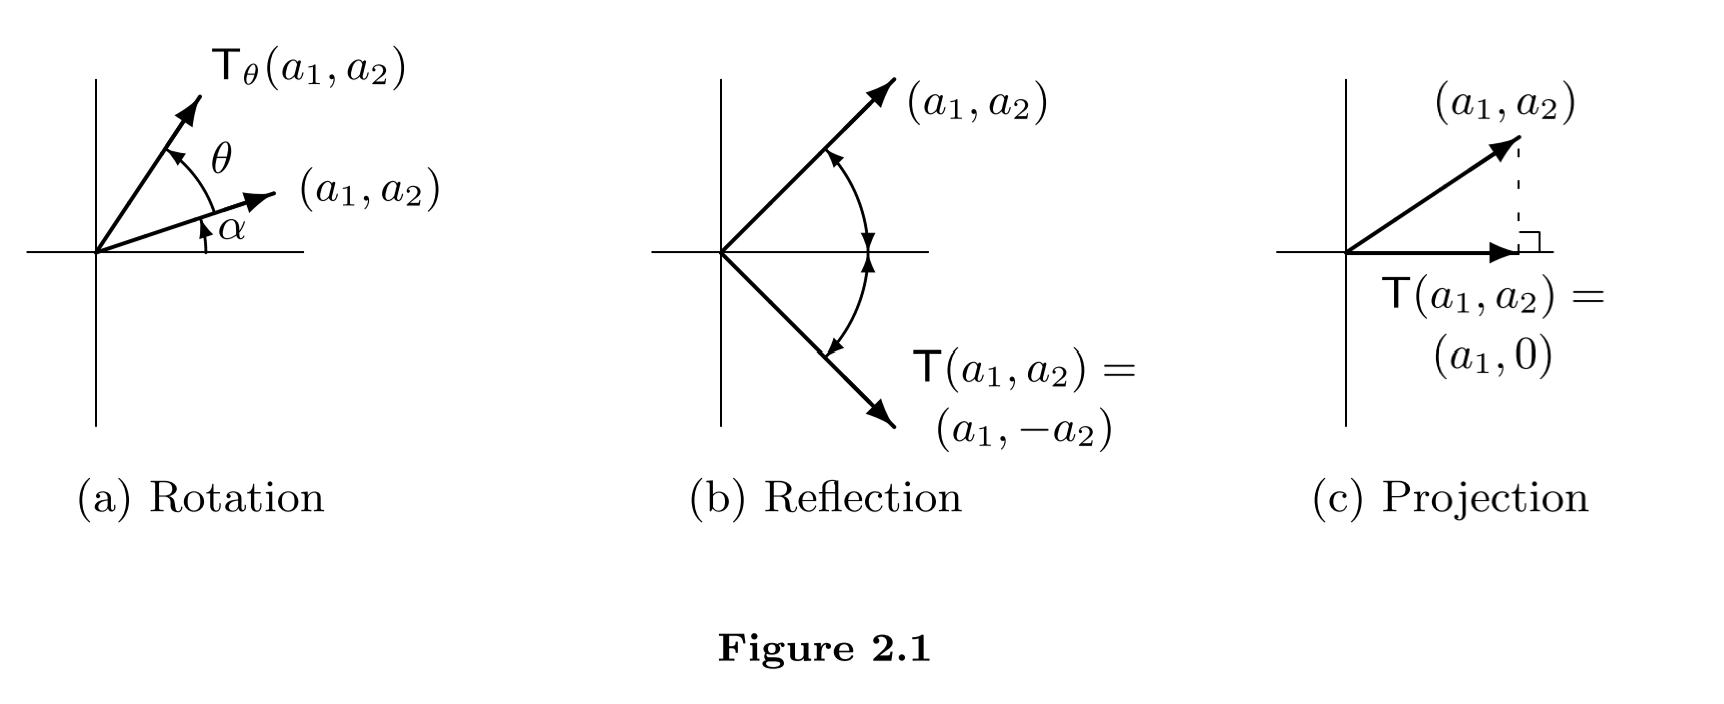
\includegraphics[width=16cm]{images/figure-2-1.png}

\begin{example} \label{example 2.1.2}
For any angle \(\theta\), define \(\T_{\theta} : \SET{R}^2 \to \SET{R}^2\) by the ``rule'':
\(\T_{\theta} (a_1, a_2)\) is the vector obtained by \emph{rotating \((a_1, a_2)\) counterclockwise by \(\theta\)} if \((a_1, a_2) \ne (0, 0)\), and \(\T_{\theta}(0, 0) = (0, 0)\).
Then \(\T_{\theta} : \SET{R}^2 \to \SET{R}^2\) is a \LTRAN{} that is called the \textbf{rotation by \(\theta\)}.

We determine an \emph{explicit formula} for \(\T_{\theta}\).
Fix a nonzero vector \((a_1, a_2) \in \SET{R}^2\).
Let \(\alpha\) be the angle that \((a_1, a_2)\) \emph{makes with the positive \(x\)-axis} (see Figure 2.1(a)),
and let \(r = \sqrt{a_1^2 + a_2^2}\).
Then \(a_1 = r \cos \alpha\) and \(a_2 = r \sin \alpha\).
Also, \(\T_{\theta}(a_1, a_2)\) has length \(r\) and makes an angle \(\alpha + \theta\) with the positive \(x\)-axis.
It follows that
\begin{align*}
    \T_{\theta}(a_1, a_2) & = (r \cos(\alpha + \theta), r \sin(\alpha + \theta)) \\
                         & = (r \cos \alpha \cos \theta - r \sin \alpha \sin \theta,  r \cos \alpha \sin \theta + r \sin \alpha \cos \theta) & \text{by high school algebra} \\
                         & = (a_1 cos \theta - a_2 \sin \theta, a_1 \sin \theta + a_2 \cos \theta). & \text{since \(r \cos \alpha = a_1, r \sin \alpha = a_2\)}
\end{align*}
And by \RMK{2.1.3}, \(\T\) is linear.
\end{example}

\begin{example} \label{example 2.1.3}
Define \(\T : \SET{R}^2 \to \SET{R}^2\) by \(\T(a_1, a_2) = (a_1, -a_2)\).
\(\T\) is called the \textbf{reflection about the \(x\)-axis}.
(See Figure 2.1(b).)
\end{example}

\begin{example} \label{example 2.1.4}
Define \(\T : \SET{R}^2 \to \SET{R}^2\) by \(\T(a_1, a_2) = (a_1, 0)\).
\(\T\) is called the \textbf{projection on the \(x\)-axis} (along \(y\)-axis, see \ADEF{2.2}).
(See Figure 2.1(c).) 
\end{example}

\begin{example} \label{example 2.1.5}
Define \(\T : M_{m \X n}(F) \to M_{n \X m}(F)\) by \(\T(A) = A^\top\), where \(A^\top\) is the transpose of \(A\).
Then \(\T\) is a \LTRAN{} by \EXEC{1.3.3}, since
\begin{align*}
    \T(aA + bB) & = (aA + bB)^\top \\
               & = aA^\top + bB^\top & \text{by \EXEC{1.3.3}} \\
               & = a\T(A) + b\T(B),
\end{align*}
hence \(\T\) is linear by \ATHM{2.1}(b).
\end{example}

\begin{example} \label{example 2.1.6}
Let \(V\) denote the set of all real-valued functions defined on the real line that \emph{have derivatives of every order}.
It is easily shown that \(V\) is a vector space over \(\SET{R}\).
(See \EXEC{1.3.16}.)
Define \(\T : V \to V\) by \(\T(f) = f'\), the derivative of \(f\).
(Note that the input of \(\T\) is itself a function(from \(\SET{R}\) to \(\SET{R}\)); the output of \(\T\) is similar.)
To show that \(\T\) is linear, let \(g, h \in V\) and \(a \in \SET{R}\).
Now
\begin{align*}
    \T(ag + h) & = (ag + h)' \\
              & = ag' + h' & \text{by Calculus} \\
              & = a\T(g) + \T(h).
\end{align*}
So by \ATHM{2.1}(b), \(\T\) is linear.
\end{example}

\begin{example} \label{example 2.1.7}
Let \(V = \mathcal{C}(\SET{R})\), the vector space of all continuous real-valued functions on \(\SET{R}\).
Let \(a, b \in \SET{R}\), \(a < b\).
Define \(\T : V \to \RED{\SET{R}}\) by
\[
    \T(f) = \int_a^b f(t) dt
\]
for all \(f \in V\).
(Note that the input of \(\T\) is a (continuous) function, the output of \(\T\) is the definite integral of that input on the interval \(a, b\).)
Then \(\T\) is a \LTRAN{} because, by Calculus, the definite integral of a linear combination of functions is the same as the linear combination of
the definite integrals of the functions.
\end{example}

\begin{additional definition} \label{adef 2.1}
For vector spaces \(V\) and \(W\) (over common \(F\)), we define the \textbf{identity transformation} \(\ITRANV: V \to \RED{V}\) by \(\ITRANV(x) = x\) for all \(x \in V\) and the \textbf{zero transformation} \(\TZERO: V \to W\) by \(\TZERO(x) = \OW\) for all \(x \in V\).
It is clear that both of these transformations are linear.
We often write \(\mathrm{I}\) instead of \(\ITRANV\).
\end{additional definition}

We now turn our attention \emph{to two very important sets associated with \LTRAN{}s}: the \textbf{range} and \textbf{null space}.
The determination of these sets allows us to examine more closely the \emph{intrinsic} properties of a \LTRAN{}.

\begin{definition} \label{def 2.2}
Let \(V\) and \(W\) be vector spaces, and let \(\T : V \to W\) be linear.
We define the \textbf{null space} (or \textbf{kernel}) \(\NULLT\) of \(\T\) to be the set of all vectors \(x\) in \(V\) such that \(\T(x) = \OW\);
that is, \(\NULLT = \{ x \in V : \T(x) = \OW \}\).

We define the \textbf{range} (or \textbf{image}) \(\RANGET\) of \(\T\) to be the subset of \(W\) consisting of all images (under \(\T\)) of vectors in \(V\);
that is, \(\RANGET = \{ \T(x) : x \in V \}\).
\end{definition}

\begin{example} \label{example 2.1.8}
Let \(V\) and \(W\) be vector spaces, and let \(\ITRANV : V \to V\) and \(\TZERO : V \to W\) be the identity and zero transformations, respectively. Then \(\NULL(\ITRANV) = \{ \OV \}\), \(\RANGE(\ITRANV) = V\), \(\NULL(\TZERO) = V\), and \(\RANGE(\TZERO) = \{ \OW \}\).
\end{example}

\begin{example} \label{example 2.1.9}
Let \(\T : \SET{R}^3 \to \SET{R}^2\) be the \LTRAN{} defined by \(\T(a_1, a_2, a_3) = (a_1 - a_2, 2a_3)\).
It is left as an exercise to verify that
\[
    \NULLT = \{ (a, a, 0) : a \in \SET{R} \} \text{ and } \RANGET = \SET{R}^2.
\].
\end{example}

\begin{remark} \label{remark 2.1.4}
In \EXAMPLE{2.1.8} and \EXAMPLE{2.1.9}, we see that the range and null space of each of the \LTRAN{}s happen to be a \emph{subspace} (of the codomain and domain, respectively).
The next result shows that this is \emph{true in general}.
\end{remark}

\begin{theorem} \label{thm 2.1}
Let \(V\) and \(W\) be vector spaces and \(T : V \to W\) be linear.
Then \(\NULLT\) and \(\RANGET\) are \textbf{subspaces} of \(V\) and \(W\) (over common \(F\)), respectively.
\end{theorem}

\begin{proof}
We prove \(\NULLT\) and \(\RANGET\) are \textbf{subspaces} of \(V\) and \(W\) by showing they satisfy the conditions in \THM{1.3}.

Since by \ATHM{2.1}(a), \(\T(\OV) = \OW\), (by \DEF{2.2}) we have that \(\OV \in \NULLT\).
Let \(x, y \in \NULLT\) and \(c \in F\).
Then
\begin{align*}
    \T(x + y) & = \T(x) + \T(y) & \text{since \(\T\) is linear} \\
              & = \OW + \OW & \text{since \(x, y \in \NULLT\)} \\
              & = \OW,
\end{align*}
so by \DEF{2.2}, \(x + y \in \NULLT\);
and
\begin{align*}
    \T(cx) & = c \T(x) & \text{since \(\T\) is linear} \\
           & = c \OW & \text{since \(x \in \NULLT\)} \\
           & = \OW.
\end{align*}
Hence by \DEF{2.2}, \(cx \in \NULLT\), so that by \THM{1.3} \(\NULLT\) is a subspace of \(V\).

Now for \(\RANGET\), because \(\T(\OV) = \OW\), we have that \(\OV \in \RANGET\).
Now let \(x, y \in \RANGE(T)\) and \(c \in F\).
Then there exist \(u\) and \(w\) in \(V\) such that \(\T(v) = x\) and \(\T(w) = y\).
So \(\T(v + w) = \T(v) + \T(w) = x + y\), and \(\T(cv) = c\T(v) = cx\). Thus \(x + y \in \RANGET\) and \(cx \in \RANGET\), so by \THM{1.3}, \(\RANGET\) is a subspace of \(W\).
\end{proof}

The next theorem provides a method for finding a \emph{spanning set} (\emph{not} necessarily a basis) for the \emph{range} of a \LTRAN{}.
With this accomplished, using the technique of \EXAMPLE{1.6.6} (or \THM{1.9}), it is easy to find a basis, which is a subset of the spanning set, for the \emph{range}.

\begin{theorem} \label{thm 2.2}
Let \(V\) and \(W\) be vector spaces, and let \(\T : V \to W\) be linear.
If \(\beta = \{ v_1, v_2 , ..., v_n \}\) is a \emph{basis} for \(V\), then
\[
    \RANGET = \spann(\T(\beta)) =^{\RED{*}} \spann(\{ \T(v_1), \T(v_2), ..., \T(v_n) \}).
\]
(\RED{*} Note that \(\T(\{ v_1, v_2 , ..., v_n \})\) is just a syntactic sugar for \(\{ \T(v_1), \T(v_2), ..., \T(v_n) \}\).)

Also note that we do \emph{not} say \(\T(\beta)\) is a basis for \(\RANGET\);
we just say it is a generating set for \(\RANGET\).
\end{theorem}

\begin{proof} Clearly (by definition of the ``image'' of an input \(v_i\)) \(\T(v_i) \in \RANGET\) for each \(i\).

So \(\{ \T(v_1), \T(v_2), ..., \T(v_n) \} \subseteq \RANGET\).
Because \(\RANGET\) is a \emph{subspace}, by \THM{1.5}(b), \(\RANGET\) contains \(\spann(\{ \T(v_1 ), \T(v_2), ..., \T(v_n) \}) = \spann(\T(\beta))\).

So we have \(\spann(\T(\beta)) \subseteq \RANGET\).

Now suppose arbitrary \(w \in \RANGET\).
Then \(w = \T(v)\) for some \(v \in V\).
Because \(\beta\) is a basis for \(V\), we have
\[
    v = \sum_{i = 1}^n a_i v_i \text{ for some \(a_1, a_2, ..., a_n \in F\)} \MAROON{(1)}.
\]
Since \(T\) is linear, it follows that
\begin{align*}
    w & = \T(v) \\
      & = \T \bigg(\sum_{i = 1}^n a_i v_i \bigg) & \text{by \MAROON{(1)}} \\
      & = \sum_{i = 1}^n a_i T(v_i), & \text{by \ATHM{2.1}(d)} \\
\end{align*}
which is a linear combination of \(\T(\beta)\), hence \(w \in \spann(\T(\beta))\).
So we have \(\RANGET \subseteq \spann(\T(\beta))\).
Hence \(\RANGET = \spann(\T(\beta))\).
\end{proof}

\begin{remark} \label{remark 2.1.5}
It should be noted that \THM{2.2} is true even if \(\beta\) is infinite, that is, \(\RANGET = \spann(\{ \T(v) : v \in \beta \})\).
(See \EXEC{2.1.34}.)
\end{remark}

\begin{example} \label{example 2.1.10}
Define the linear(need to prove, but trivial) transformation \(T : \mathcal{P}_2(\SET{R}) \to M_{2 \X 2}(\SET{R})\) by
\[
    T(f) = \begin{pmatrix}
        f(1) - f(2) &    0 \\
        0           & f(0)
    \end{pmatrix}.
\]
Since \(\beta = \{1, x, x^2\}\) is a basis for \(\mathcal{P}_2(\SET{R})\), we have
\begin{align*}
    \RANGET & = \spann(\T(\beta)) & \text{by \THM{2.2}} \\
            & = \spann(\{\T(1), \T(x), \T(x^2)\}) & \text{unwrap syntactic sugar} \\
            & = \spann\bigg(\bigg\{
                    \begin{pmatrix}
                        0 & 0 \\
                        0 & 1
                    \end{pmatrix},
                    \begin{pmatrix}
                        -1 & 0 \\
                        0  & 0
                    \end{pmatrix},
                    \begin{pmatrix}
                        -3 & 0 \\
                        0  & 0
                    \end{pmatrix}
                \bigg\}\bigg) \\
            & = \spann\bigg(\bigg\{
                    \begin{pmatrix}
                        0 & 0 \\
                        0 & 1
                    \end{pmatrix},
                    \begin{pmatrix}
                        -1 & 0 \\
                        0  & 0
                    \end{pmatrix}
                \bigg\}\bigg) & \text{by extract subset as basis}
\end{align*}
Thus we have found a basis for \(\RANGET\), and so \(\dim(\RANGET) = 2\).

Now suppose that we want to find a basis for \(\NULLT\).
Note that \(f \in \NULLT\) if and only if \(T(f) = O_{2 \X 2}\), the \(2 \X 2\) zero matrix.
That is, \(f \in \NULLT\) if and only if
\[
    \begin{pmatrix}
        f(1) - f(2) & 0 \\
        0 & f(0)
    \end{pmatrix}
    = \begin{pmatrix}
        0 & 0 \\
        0 & 0
    \end{pmatrix}.
\]
Now express \(f(x) = a + bx + cx^2\) for any \(a, b, c \in \SET{R}\).
If \(f(1) - f(2) = 0\) and \(f(0) = 0\), then we have \(0 = f(1) - f(2) = (a + b + c) - (a + 2b + 4c) = -b - 3c\), or \(b = -3c\);
and \(0 = f(0) = a + 0 + 0 = a\).
So \(f\) must have the form that \(f(x) = 0 + (-3c) x + c x^2 = c(-3x + x^2)\).
Hence \(\NULLT = \{ c(-3x + x^2) : c \in \SET{R} \}\), and trivially the basis is \(\{ -3x + x^2 \}\), hence \(\NULLT\) has dimension \(1\).
\end{example}

\begin{remark} \label{remark 2.1.6}
Note that in \EXAMPLE{2.1.10},
\[
    \dim(\NULLT) + \dim(\RANGET) = 1 + 2 = 3 = \dim(\mathcal{P}_2(\SET{R})).
\]
In \THM{2.3}, we see that a similar result is \emph{true in general}.
\end{remark}

As in \CH{1}, we ``measure the size'' of a subspace by its dimension.
The null space and range are so important that we \emph{attach special names} to their respective dimensions.

\begin{definition} \label{def 2.3}
Let \(V\) and \(W\) be vector spaces, and let \(\T : V \to W\) be linear.
If \(\NULLT\) and \(\RANGET\) are finite-dimensional, then we define the \textbf{nullity} of \(\T\), denoted \(\nullityT\), and the \textbf{rank} of \(\T\), denoted \(\rankT\),
to be the dimensions of \(\NULLT\) -- or \(\dim(\NULLT)\) -- and \(\RANGET\) -- or \(\dim(\RANGET)\) -- respectively.
\end{definition}

\begin{remark} \label{remark 2.1.7}
Reflecting on the action of a \LTRAN{}, we see intuitively that \textbf{the larger the nullity, the smaller the rank}.
In other words, the more vectors that are carried into \(\OW\), the smaller the range.
The same heuristic reasoning tells us that \textbf{the larger the rank, the smaller the nullity}.
This balance between rank and nullity is made precise in the next theorem, appropriately called \textbf{the dimension theorem}.
\end{remark}

\begin{theorem} [Dimension Theorem] \label{thm 2.3}
Let \(V\) and \(W\) be vector spaces, and let \(\T : V \to W\) be linear.
If \(V\) is \emph{finite}-dimensional, then
\[
    \nullityT + \rankT = \dim(V).
\]
\end{theorem}

\begin{proof}
Suppose that \(\dim(V) = n, \nullityT = k\), and \(\{ v_1, v_2, ..., v_k \}\) is a basis for \(\NULLT\).
By \CORO{1.11.1}, (since \(\NULLT\) is a subspace of \(V\),) we may extend \(\{ v_1, v_2, ..., v_k \}\) to a basis \(\beta = \{ v_1, v_2, ..., v_k, v_{k +1}, ..., v_n \}\) for \(V\).
We claim that
\[
    S = \{ \T(v_{k + l}), \T((v_{k + 2}), ..., \T(v_n) \}
\]
is a basis for \(\RANGET\).

But first, we need to show that \(\T(v_{k + 1}), ..., \T(v_n)\) are all \textbf{distinct}. (s.t. \(S\) has \(n - k\) elements.)

For the sake of contradiction, suppose not.
Then there exists \(i \ne j\), \(k + 1 \le i \le n, k + 1 \le j \le n\), s.t. \(\T(v_i) = \T(v_j)\).
And
\begin{align*}
             & \T(v_i) = \T(v_j) \\
    \implies & \T(v_i) - \T(v_j) = \OW \\
    \implies & \T(v_i - v_j) = \OW & \text{by \ATHM{2.1}(c)} \\
    \implies & v_i - v_j \in \NULLT & \text{by \DEF{2.2}} \\
    \implies & v_i - v_j \in \spann(\{ v_1, ..., v_k \}) \\
    \implies & \{ v_1, ..., v_k, v_i - v_j \} \text{ is \LDP{} } & \text{by \THM{1.7}}
\end{align*}
So we have a \emph{nontrivial} combination \(\OV = a_1 v_1 + ... + a_k v_k + a (v_i - v_j)\).
Note that \(a\) cannot be zero, otherwise one of \(a_1, ..., a_k\) must be nonzero and we have nontrivial representation using \(v_1, ..., v_k\), which contradicts that \(v_1, ..., v_k\) is \LID{}.
But then \(\OV = a_1 v_1 + ... + a_k v_k + a (v_i - v_j) = a_1 v_1 + ... + a_k v_k + a v_i - a v_j\), and that still implies \(\{ a_1, a_2, ..., a_k, a_i, a_j \}\) are \LDP{}, which is a contradiction since it is a subset of a basis (hence \LID{}) of \(V\).
So \(\T(v_{k + 1}), \T(v_{k + 2}), ..., \T(v_n)\) must be all distinct, so \(S\) really has \(n - k\) elements.

Go back to the consideration of \(S\).
First we prove that \(S\) generates \(\RANGET\).
Using \THM{2.2} (and \(\beta\) is a basis for \(V\)) and \RED{the fact that} \(\T(v_i) = \OW\) for \(1 \le i \le k\), we have
\begin{align*}
    \RANGET & = \spann(\{ \T(v_1), \T(v_2), ..., \T(v_{k}), \T(v_{k + 1}, ..., T(v_n) \}) & \text{by \THM{2.2}} \\
            & = \spann(\{ \OW, \OW, ..., \OW, \T(v_{k + 1}), ..., \T(v_{n}) \}) & \text{using the fact} \\
            & = \spann(\{ \OW, \T(v_{k + 1}), ..., \T(v_{n}) \}) & \text{equal by set theory} \\
            & = \spann(\{ \T(v_{k + 1}), ..., \T(v_{n}) \}) & \text{of course, by \CH{1}} \\
            & = \spann(S).
\end{align*}

Now we prove that \(S\) is \LID{}.
So suppose that
\[
    \sum_{i = k + 1}^n b_i T(v_i) = \OW \text{ for some scalars \(b_{k + 1}, ..., b_n \in F\)}. \MAROON{(1)}
\]
Using the fact that \(T\) is linear, by \ATHM{2.1}(d), we have
\[
    T\bigg( \sum_{i = k + 1}^n b_i v_i \bigg) = \OW.
\]
So by \DEF{2.2},
\[
    \sum_{i = k + 1}^n b_i v_i \in \NULLT.
\]
Hence \(LHS\) can be represented as a linear combination of the basis of \(\NULLT\), that is,
\[
    \sum_{i = k + 1}^n b_i v_i = \sum_{i = 1}^k c_i v_i,
\]
hence
\[
    \sum_{i = 1}^k (-c_i) v_i + \sum_{i = k + 1}^n b_i v_i = \OV.
\]
But \(\beta = \{ v_1, ..., v_k, v_{k + 1}, ..., v_n \}\) is known to be the basis of \(V\) (hence is \LID{}), so we have \(c_i\) for \(i = 1, ..., k\) and \(b_i\) for \(i = k + 1, ..., n\) are all equal to zero.
And in particular, \(b_{k + 1} = ... = b_n = 0\).
So by \MAROON{(1)}, \(S\) is \LID{}.

Hence we know \(S\) generates \(\RANGET\) and is \LID{}, so \(S\) is a basis for \(\RANGET\).
Therefore \(\rankT = \#S = n - k\), there for \(\nullityT + \rankT = k + (n - k) = n = \dim(V)\).
\end{proof}

\begin{note}
If we apply the dimension theorem to the \LTRAN{} \(\T\) in \EXAMPLE{2.1.9}, we have that \(\nullityT + 2 = 3\), so \(\nullityT = 1\).
\end{note}

\begin{remark} \label{remark 2.1.8}
The reader should review the concepts of \emph{``one-to-one'' and ``onto''}.
Interestingly, for a \LTRAN{}, both of these concepts are \emph{intimately connected} to the rank and nullity of the transformation.
This is demonstrated in the next two theorems.
\end{remark}

\begin{theorem} \label{thm 2.4}
Let \(V\) and \(W\) be vector spaces, and let \(\T : V \to W\) be linear.
Then \(\T\) is one-to-one \emph{if and only if} \(\NULLT = \{ \OV \}\).
\end{theorem}

\begin{proof} \ 

\(\Longrightarrow\): Suppose \(\T\) is one-to-one, we have to show \(\NULLT = \{ \OV \}\).
So let \(x \in \NULLT\), we have to show \(x = \OV\).
By \DEF{2.2}, we have \(\T(x) = \OW\).
But by \ATHM{2.1}(a), \(\T(\OV) = \OW\).
So we have \(\T(x) = \T(\OV)\).
By definition of one-to-one, that implies \(x = \OV\).

\(\Longleftarrow\):
Suppose \(\NULLT = \{ \OV \}\), we have to show \(\T\) is one-to-one.
So suppose arbitrary \(x_1, x_2\) s.t. \(\T(x_1) = \T(x_2)\), we have to show \(x_1 = x_2\).
Then we have
\begin{align*}
             & \T(x_1) = \T(x_2) \\
    \implies & \T(x_1) - \T(x_2) = \OW \\
    \implies & \T(x_1 - x_2) = \OW & \text{by \ATHM{2.1}(c)} \\
    \implies & x_1 - x_2 \in \NULLT & \text{by \DEF{2.2}} \\
    \implies & x_1 - x_2 = \OV & \text{since \(\NULLT = \{ \OV \}\)} \\
    \implies & x_1 = x_2.
\end{align*}
So by definition, \(\T\) is one-to-one.
\end{proof}

\begin{remark} \label{remark 2.1.9}
\THM{2.4} is true even if \(V\) is \emph{infinite}-dimensional.
\end{remark}

\begin{note}
Observe that \THM{2.4} allows us to conclude that the transformation defined in \EXAMPLE{2.1.9} is not one-to-one since \(\NULLT \ne \{ \OV \}\).
\end{note}

Surprisingly, the conditions of one-to-one and onto are \textbf{equivalent} in an important special case; that is, when the domain and codomain of the \LTRAN{} have the same \emph{finite} dimensions.

\begin{theorem} \label{thm 2.5}
Let \(V\) and \(W\) be \emph{finite}-dimensional vector spaces \textbf{of equal dimension}, and let \(\T : V \to W\) be linear.
Then the following are equivalent.
\begin{enumerate}
\item \(\T\) is one-to-one.
\item \(T\) is onto.
\item \(\rankT = \dim(V)\).
\end{enumerate}
\end{theorem}

\begin{proof}
From the dimension theorem \THM{2.3}, we have
\[
    \nullityT + \rankT = \dim(V). \MAROON{(1)}
\]
And we have
\begin{align*}
         & \BLUE{\T \text{ is one-to-one }} \\
    \iff & \NULLT = \{ \OV \} & \text{by \THM{2.4}} \\
    \iff & \nullityT = 0 & \text{by \DEF{2.3}} \\
    \iff & \BLUE{\rankT = \dim(V)} & \text{by \MAROON{(1)}} \\
    \iff & \rankT = \dim(W) & \text{since \(V\) and \(W\) have same finite-dimension} \\
    \iff & \dim(\RANGET) = \dim(W) & \text{by \DEF{2.3}} \\
    \iff & \RED{*} \BLUE{\T \text{ is onto.}}
\end{align*}
So we have shown (a), (b), and (c) are equivalent.

\RED{*}: For the last step, since by \THM{2.1}, \(\RANGET\) is a subspace of \(W\), and has the same dimension with \(W\), by \THM{1.11}, \(\RANGET = W\), which implies \(\T\) is onto.
\end{proof}

\begin{remark} \label{remark 2.1.10}
We note that if \(V\) is \emph{not} finite-dimensional and \(\T : V \to V\) is linear, then \textbf{it does not follow that} one-to-one and onto are equivalent.
(See \EXEC{2.1.15}, \EXEC{2.1.16}, and \EXEC{2.1.21}.)

Note that the \textbf{linearity} of \(\T\) in \THM{2.4} and \THM{2.5} is essential, for it is easy to construct examples of functions from \(\SET{R}\) into \(\SET{R}\) that are not one-to-one, but
are onto, and vice versa.
\end{remark}

\begin{example} \label{example 2.1.11}
Let \(\T : \mathcal{P}_2(\SET{R}) \to \mathcal{P}_3(\SET{R})\) be the \LTRAN{} defined by
\[
    \T(f(x)) = 2f'(x) + \int_0^x 3f(t) dt.
\]
(Note that integration will make the degree increase by \(1\), so the codomain has one more dimension than domain.)

Now
\begin{align*}
    \RANGET & = \spann(\{ \T(1), \T(x), \T(x^2) \}) & \text{by \THM{2.2}} \\
            & = \spann(\{ 3x, 2 + \frac{3}{2} x^2, 4x + x^3 \}).
\end{align*}
Since \(\{ 3x, 2 + \frac{3}{2} x^2, 4x + x^3 \}\) is \LID{}, \(\rankT = 3\).
Since the dimension of the codomain \(\dim(\mathcal{P}_3(\SET{R})) = 4\), \(\T\) is not onto.
From the dimension theorem, \(3 = \dim(\mathcal{P}_2(\SET{R})) = \nullityT + \rankT = \nullityT + 3\).
So \(\nullityT = 0\), and therefore, \(\NULLT = \{ \OV \}\).
We conclude from \THM{2.4} that \(\T\) is one-to-one.
\end{example}

\begin{example} \label{example 2.1.12}
Let \(\T : F^{\RED{2}} \to F^{\RED{2}}\) be the \LTRAN{} defined by
\[
    \T(a_1, a_2) = (a_1 + a_2, a_1).
\]
It is easy to see that \(\NULLT = \{ \OV \}\);
so by \THM{2.4} \(\T\) is one-to-one.
Hence \THM{2.5} tells us that (since domain and codomain of \(\T\) have same finite dimension,) \(\T\) must be onto.
\end{example}

\begin{note}
In \EXEC{2.1.14}, it is stated that if \(\T\) is linear and one-to-one, then a subset \(S\) (of domain of \(\T\)) is \LID{} if and only if \(\T(S)\) (, a subset of codomain of \(\T\),) is \LID{}.
The next example illustrates the use of this result.
\end{note}

\begin{example} \label{example 2.1.13}
Let \(\T : \mathcal{P}_2(\SET{R}) \to \SET{R}^3\) be the \LTRAN{} defined by
\[
    \T(a_0 + a_1 x + a_2 x^2) = (a_0, a_1, a_2).
\]
Clearly \(\T\) is linear and one-to-one(and onto).
Let \(S = \{ 2 - x + 3x^2, x + x^2, 1 - 2x^2 \}\).
Then \(S\) is \LID{} in \(\mathcal{P}_2(\SET{R})\) because (by \EXEC{2.1.14} and)
\[
    \T(S) = \{ (2, -1, 3), (0, 1, 1), (1, 0, -2) \}
\]
is \LID{} in \(\SET{R}^3\).
\end{example}

\begin{remark} \label{remark 2.1.11}
In \EXAMPLE{2.1.13}, we \emph{transferred a property} from the vector space of polynomials (with dimension \(3\)) to a property in the vector space of \(3\)-tuples (also with dimension \(3\)).
This technique is exploited more fully later.
(See \SEC{2.4}).
\end{remark}

\begin{note}
\EXEC{2.1.14} 的用意是,你想看一坨向量是否線性獨立,但(可能)很難算,於是你把它們用一個符合一對一的線性函數\ \(\T\) 變換成另一個空間的一坨向量,並且在該空間計算向量是否線性獨立(可能)比較好算;算完後再根據\ \EXEC{2.1.14} 就可知道原本那陀向量是否線性獨立了。
\end{note}

One of the most important properties of a \LTRAN{} is that \textbf{it is completely determined by its action on a basis}.
This result, which follows from the next theorem and corollary, is used frequently throughout the book.

\begin{theorem} \label{thm 2.6}
Let \(V\) and \(W\) be vector spaces over \(F\), and suppose that \(\{ v_1, v_2, ..., v_n \}\) is a basis for \(V\).
Then given any \(n\) vectors \(w_1, w_2, ..., w_n \in W\), there \textbf{exists exactly one} \LTRAN{} \(\T : V \to W\) such that \(\T(v_i) = w_i\) for \(i= 1, 2, ..., n\).
\end{theorem}

\begin{remark} \label{remark 2.1.12}
The purpose of \THM{2.6} is that, if \(V\) and \(W\) are finite vector spaces, and given any \emph{basis} \(\{ v_1, v_2, ..., v_n \}\) for \(V\), and the ``wanted'' corresponding output \(\{ w_1, w_2, ..., w_n \}\) in \(W\), we \emph{can always find} a \LTRAN{} from \(V\) to \(W\) that satisfies the requirement.
Furthermore, the found \LTRAN{} \emph{is unique}.

Hence we can just use a ``mapping'' \(v_1 \to w_1, v_1 \to w_2, ..., v_n \to w_n\) to \emph{identify} the one and only one \LTRAN{}, so this identification is \emph{well-defined}.
And in later sections, we will learn that the ``mapping'' can be represented using \textbf{matrix}!
And that ultimately implies that every \LTRAN{} corresponds to a unique matrix.
\end{remark}

\begin{proof}
Let \(\{ v_1, v_2, ..., v_n \}\) be a basis for \(V\), and let \(w_1, w_2, ..., w_n\) be vectors in \(W\).

We first prove the existence of \(\T\) such that \(\T\) is linear and \(\T(v_i) = w_i\) for \(i = 1, 2, ..., n\).

So suppose arbitrary \(x \in V\).
Then (since \(\{ v_1, ..., v_n \}\) is a basis for \(V\),)
\[
    x = \sum_{i = 1}^n a_i v_i,
\]
where \(a_1, ..., a_n\) are \textbf{unique} scalars.
Now we prove by construction by defining \(\T\), using this scalars \emph{that depend on \(x\)}:
\[
    \T : V \to W \text{ by } \T(x) = \T\bigg(\sum_{i = 1}^n a_i v_i\bigg) = \sum_{i = 1}^n a_i w_i. \MAROON{(1)}
\]
Then of course \(\T\) is really a \emph{well-defined} function, since
\BLUE{(1)} it's output is a linear combination of \(W\)'s vectors, which must be in \(W\);
\BLUE{(2)} And since for any \(x\) in \(V\), the corresponding scalars \(a_1, ..., a_n\) are \emph{unique}, hence the output of \(\T\) is also unique.
Also note that \MAROON{(1)} is \textbf{not} actually a ``formula'' with ``constant scalars'' \(a_1, ..., a_n\), since \(a_1, ..., a_n\) are determined by (or dependent on) the given \(x\), so they are ``dynamic''.

Then we have to show (a) \(\T\) is linear; (b) \(\T(v_i) = w_i\) for all \(i = 1, ..., n\):
\begin{enumerate}
\item
We will use \ATHM{2.1}(b) to show \(\T\) is linear.
So suppose \(u, v \in V\), and \(d \in F\).
Then (similarly as \(x \in V\),) we may write
\[
    u = \sum_{i = 1}^n b_i v_i \text{ and } v = \sum_{i = 1}^n c_i v_i \MAROON{(2)}
\]
for some (unique) scalars \(b_1, b_2, ..., b_n\) and \(c_1, c_2, ..., c_n\).
Thus
\begin{align*}
    d u + v & = d \sum_{i = 1}^n b_i v_i + \sum_{i = 1}^n c_i v_i \\
            & = \sum_{i = 1}^n (db_i + c_i) v_i \MAROON{(3)} & \text{by rules of finite summation}
\end{align*}
So
\begin{align*}
    \T(du + v) & = \T\bigg( \sum_{i = 1}^n (db_i + c_i) v_i \bigg) & \text{by \MAROON{(3)}} \\
               & = \sum_{i = 1}^n (db_i + c_i) w_i \\
               & \text{\ \ \ \ \ \ (by \MAROON{(1)}; note that now the corresponding} \\
               & \text{\ \ \ \ \ \ \ \ scalars \(a_1, ..., a_n\) in \MAROON{(1)}} \\
               & \text{\ \ \ \ \ \ \ \ are \(d b_1 + c_1, ..., d b_n + c_n\))} \\
               & = d \sum_{i = 1}^n b_i w_i + \sum_{i = 1}^n c_i w_i & \text{by rules of finite summation} \\
               & = d \T\bigg( \sum_{i = 1}^n b_i v_i \bigg) + \T\bigg( \sum_{i = 1}^n c_i v_i \bigg) & \text{again by \MAROON{(1)}} \\
               & = d \T(u) + \T(v), & \text{by \MAROON{(2)}}
\end{align*}
hence \(\T\) is linear.

\item
For \(v_i\) where \(i = 1, ..., n\):
\begin{align*}
    \T(v_i) & = \T(0 v_1 + ... + 1 v_i + ... + 0 v_n) & \text{in particular} \\
            & = 0 w_1 + ... + 1 w_i + ... + 0 w_n & \text{by \MAROON{(1)}, and expand summation} \\
            & = w_i.
\end{align*}
\end{enumerate}
Hence \(\T\) satisfies the two requirements, so the existent part is proved.

Now we have to show \(\T\) is unique.
So suppose \(\U\) is also linear s.t. \(\U(v_i) = w_i\) for \(i = 1, ..., n\).
We have to show \(\U = \T\);
that is, (by definition of function equality,) we have to show \(\forall x \in V, \U(x) = \T(x)\).

But for each \(x \in V\), where again we represent \(x = \sum_{i = 1}^n a_i v_i\) for unique scalars \(a_1, ..., a_n\) \MAROON{(4)},
\begin{align*}
    \U(x) & = \U\bigg(\sum_{i = 1}^n a_i v_i\bigg) & \text{by \MAROON{(4)}}\\
           & = \sum_{i = 1}^n a_i \U(v_i) & \text{since \(\U\) is linear} \\
           & = \sum_{i = 1}^n a_i w_i & \text{since also \(\U(v_i) = w_i\)} \\
           & = \T\bigg(\sum_{i = 1}^n a_i v_i\bigg) & \text{by \MAROON{(1)}} \\
           & = \T(x). & \text{by \MAROON{(4)}}
\end{align*}
So \(\U = \T\), as desired.
\end{proof}

\begin{note}
There is \href{https://www.youtube.com/watch?v=gAlUekIYKLA&ab_channel=DrPeyam}{another proof} for \THM{2.6}.
\end{note}

\begin{corollary} \label{corollary 2.6.1}
\sloppy Let \(V\) and \(W\) be vector spaces, and suppose that \(V\) has a finite basis \(\{ v_1, v_2, ..., v_n \}\).
If \(\U, \T : V \to W\) are linear and \(\U(v_i) = \T(v_i)\) for \(i = 1, 2, ..., n\), then \(\U = \T\).
\end{corollary}

\begin{proof}
Well, since by \THM{2.6} \emph{the} \LTRAN{} that satisfies the mapping \(v_i \to w_i\) for \(i = 1, 2, ... n\) is unique,
and both \(\U, \T\) are linear and satisfy the mapping, hence they are equal to that unique \LTRAN{} hence are equal to each other.
\end{proof}

\begin{example} \label{example 2.1.14}
Let \(\T : \SET{R}^2 \to \SET{R}^2\) be the \LTRAN{} defined by
\[
    \T(a_1, a_2) = (2 a_2 - a_1, 3 a_1),
\]
Then \(\T(1, 2) = (3, 3)\) and \(\T(1, 1) = (1, 3)\), where \(\{ (1, 2), (1, 1) \}\) is a basis for \(\SET{R}^2\).
Now suppose that \(\U : \SET{R}^2 \to \SET{R}^2\) is linear.
If we know that \(\U(1, 2) = (3, 3)\) and \(\U(1, 1) = (1, 3)\), then by \CORO{2.6.1}, \(\U = \T\).
\end{example}

\exercisesection

\begin{exercise} \label{exercise 2.1.1}
Label the following statements as true or false.
In each part, \(V\) and \(W\) are \textbf{finite}-dimensional vector spaces (over common \(F\)), and \(\T\) is a function from \(V\) to \(W\).
\begin{enumerate}
\item If \(\T\) is linear, then \(\T\) preserves sums and scalar products.
\item If \(\T(x + y) = \T(x) + \T(y)\). then \(\T\) is linear.
\item \(\T\) is one-to-one if and only if the only vector \(x\) such that \(\T(x) = \OW\) is \(x = \OV\).
\item If \(\T\) is linear, then \(\T(\OV) = \OW\).
\item If \(\T\) is linear, then \(\nullityT + \rankT = \dim(W)\).
\item If \(\T\) is linear, then \(\T\) carries \LID{} subsets of \(V\) onto \LID{} subsets of \(W\).
\item If \(\T, \U : V \to W\) are both linear and agree on a basis for \(V\), then \(\T = \U\).
\item Given \(x_1, x_2 \in V\) and \(y_1, y_2 \in W\), there exists a \LTRAN{} \(\T : V \to W\) such that \(\T(x_1) = y_1\) and \(\T(x_2) = y_2\).
\end{enumerate}
\end{exercise}

\begin{proof} \ 
\begin{enumerate}
\item I really don't know what does the problem want to say, but others say it's true.
\item No, \(\T\) must also need to satisfy \DEF{2.1}(b).
\item False, that is true (by \THM{2.4}) only when we know \(\T\) is linear.
\item True by \ATHM{2.1}(a).
\item False, by \THM{2.3}, \(\nullityT + \rankT = \dim(V)\).
\item False, zero transformation, which is linear, carries all vectors into \(\OW\), which is itself \LDP{}.
    But this is true if \(\T\) is also one-to-one, see \EXEC{2.1.14}.
\item True by \THM{2.6}(or \CORO{2.6.1}).
\item False.
    We can easily find a counterexample when \(x_1, x_2\) are \LDP{}: Let \(V = W = \SET{R}^2\) and \(x_1 = (1, 0), x_2 = (2, 0), y_1 = (1, 0), y_2 = (0, 1)\).
    Then suppose arbitrary \(\T : V \to W\) s.t. \(\T\) is linear, and suppose \(\T(1, 0) = (1, 0)\), that is, \(\T(x_1) = y_1\).
    Then
    \begin{align*}
        \T(x_2) & = \T(2, 0) \\
                & = \T(2(1, 0)) \\
                & = 2\T(1, 0) & \text{since \(\T\) is linear} \\
                & = 2(1, 0) & \text{by supposition} \\
                & = (2, 0) \ne (0, 1) = y_2,    
    \end{align*}
    so any linear \(\T\) can never satisfy the requirement.
\end{enumerate}
\end{proof}

\begin{note}
Exercises 2 - 5 are calculation problems, it's good practice, but it's painful using \LaTeX, skip.
\end{note}

\setcounter{exercise}{5}

\begin{exercise} \label{exercise 2.1.6}
\(\T : M_{n \X n}(F) \to F\) defined by
\[
    \T(A) = \TRACE(A) = \sum_{i = 1}^n A_{ii}.
\]
\end{exercise}

\begin{proof}
\(\NULLT\) is the set of all \(n \X n\) matrices with trace equal to \(0\).
By \ATHM{1.19}(a), \(\nullityT = n^2 - 1\).
And it's trivial that \(\rankT = 1\).
So \(\dim(M_{n \X n}(F)) = n^2 = (n^2 - 1) + 1 = \nullityT + \rankT\), as desired.
And since \(\NULLT \ne \{ \OV \}\), by \THM{2.4}, \(\T\) is not one-to-one.
And since \(\rankT = \dim(W)\), which implies \(\RANGET = W\), \(\T\) is onto.
\end{proof}

\begin{exercise} \label{exercise 2.1.7}
Prove properties 1, 2, 3, and 4 on page 65.
\end{exercise}

\begin{proof}
See \ATHM{2.1}.
\end{proof}

\begin{exercise} \label{exercise 2.1.8}
Prove rotation, reflection, and projection on \EXAMPLE{2.1.2}, \EXAMPLE{2.1.3} are linear.
\end{exercise}

\begin{proof} \ 

\begin{enumerate}
\item
By \EXAMPLE{2.1.2}, given any \(\theta\), we have rotation formula
\[
    \T_{\theta}(a_1, a_2) = (a_1 \cos \theta - a_2 \sin \theta, a_1 \sin \theta + a_2 \cos \theta).
\]
And
\begin{align*}
    & \ \T_{\theta}(c(a_1, a_2) + (b_1, b_2)) \\
    & = \T_{\theta}(ca_1 + b_1, ca_2 + b_2) \\
    & \text{\ \ \ \ \ \ (combining coordinates)} \\
    & = \big( (ca_1 + b_1) \cos \theta - (ca_2 + b_2) \sin \theta, (ca_1 + b_1) \sin \theta + (ca_2 + b_2) \cos \theta \big) \\
    & \text{\ \ \ \ \ \ (by def of \(\T_{\theta}\))} \\
    & = c(a_1 \cos \theta - a_2 \sin \theta, a_1 \sin \theta + a_2 \cos \theta) + (b_1 \cos \theta - b_2 \sin \theta, b_1 \sin \theta + b_2 \cos \theta) \\
    & \text{\ \ \ \ \ \ (splitting coordinates)} \\
    & = c\T(a_1, a_2) + \T(b_1, b_2) \\
    & \text{\ \ \ \ \ \ (by def of \(\T_{\theta}\))}
\end{align*}
So by \ATHM{2.1}(b), \(\T\) is linear.


\item
By \EXAMPLE{2.1.3}, the reflection (about \(x\)-axis) is
\[
    \T(a_1, a_2) = (a_1, -a_2).
\]
Then
\begin{align*}
    & \ \T(c(a_1, a_2) + (b_1, b_2)) \\
    & = \T(ca_1 + b_1, ca_2 + b_2) \\
    & = (ca_1 + b_1, -(ca_2 + b_2)) & \text{by def of \(\T\)} \\
    & = c(a_1, -a_2) + (b_1, -b_2) & \text{splitting coordinates} \\
    & = c\T(a_1, a_2) + \T(b_1, b_2), & \text{by def of \(T\)}
\end{align*}
So by \ATHM{2.1}(b), \(\T\) is linear.

\item
By \EXAMPLE{2.1.4}, the projection (on \(x\)-axis) is
\[
    \T(a_1, a_2) = (a_1, 0).
\]
Then
\begin{align*}
    & \ \T(c(a_1, a_2) + (b_1, b_2)) \\
    & = \T(ca_1 + b_1, ca_2 + b_2) \\
    & = (ca_1 + b_1, 0) & \text{by def of \(\T\)} \\
    & = c(a_1, 0) + (b_1, 0) & \text{splitting coordinates} \\
    & = c\T(a_1, a_2) + \T(b_1, b_2), & \text{by def of \(T\)}
\end{align*}
So by \ATHM{2.1}(b), \(\T\) is linear.
\end{enumerate}
\end{proof}

\begin{exercise} \label{exercise 2.1.9}
In this exercise, \(\T : \SET{R}^2 \to \SET{R}^2\) is a \emph{function}.
For each of the following parts, state why \(\T\) is \emph{not} linear.
\begin{enumerate}
\item \(\T(a_1 , a_2) = (1, a_2)\)
\item \(\T(a_1, a_2) = (a_1, a_1^2)\)
\item \(\T(a_1, a_2) = (\sin a_1, 0)\)
\item \(\T(a_1, a_2) = (\abs{a_1}, a_2)\)
\item \(T(a_1, a_2) = (a_1 + 1, a_2)\)
\end{enumerate}
\end{exercise}

\begin{proof}
By \RMK{2.1.3}, it is immediately seen that all of them are \emph{not} linear.
The particular reasons are:
\begin{enumerate}
\item \(T(0, 0) = (1, 0) \ne \OW\), violating \ATHM{2.1}(a) hence is not linear.
\item \(\T((1, 0) + (1, 0)) = \T(2, 0) = (2, 4)\), but \(\T(1, 0) + \T(1, 0) = (1, 1) + (1, 1) = (2, 2) \ne (2, 4)\), violating \DEF{2.1}(a).
\item \(\T((x, 0) + (y, 0)) = \T(x + y, 0) = (\sin (x + y), 0) = (\sin x \cos y + \cos x \sin y, 0)\) \MAROON{(1)},
    but \(\T(x, 0) + \T(y, 0) = (\sin x, 0) + (\sin y, 0) = (\sin x + \sin y, 0)\),
    which is not necessarily equal to \MAROON{(1)}, so \DEF{2.1}(a) is violated.
\item \(\T(-1(-5, 0)) = \T(5, 0) = (5, 0)\) but \(-1\T(-5, 0) = -1(5, 0) = (-5, 0)\), so \DEF{2.1}(b) is violated.
\item \(\T(0, 0) = (1, 0) \ne \OW\), violating \ATHM{2.1}(a), hence is not linear.
\end{enumerate}
\end{proof}

\begin{exercise} \label{exercise 2.1.10}
Suppose that \(\T : \SET{R}^2 \to \SET{R}^2\) is \emph{linear}, \(\T(1, 0) = (1, 4)\), and \(\T(1, 1) = (2, 5)\).
What is \(\T(2, 3)\)?
Is \(\T\) one-to-one?
\end{exercise}

\begin{proof}
Since \(\{ (1, 0), (1, 1) \}\) is (trivially) a basis for \(\SET{R}^2\), by \THM{2.6} the \(\T\) is \emph{already uniquely determined}.
And
\begin{align*}
    \T(2, 3) & = \T(-1(1, 0) + 3(1, 1)) & \text{of course} \\
             & = -1\T(1, 0) + 3\T(1, 1) & \text{since \(\T\) is linear} \\
             & = -1(1, 4) + 3(2, 5) \\
             & = (5, 11).
\end{align*}
Now by \THM{2.2}, \(\RANGET = \spann(\{ \T(1, 0), \T(1, 1) \}) = \spann(\{ (1, 4), (2, 5) \}\).
Since \(\{ (1, 4), (2, 5) \}\) is \LID{}, it is a basis for \(\RANGET\), hence \(\rankT = 2\).
By \THM{2.3}, \(\nullityT = \dim(V) - \rankT = 2 - 2 = 0\), so \(\NULLT = \{ \OV \}\);
by \THM{2.4}, \(\T\) is one-to-one.
(Also since domain and codomain of \(\T\) have same finite dimension, by \THM{2.5} \(\T\) is also onto.)
\end{proof}

\begin{exercise} \label{exercise 2.1.11}
Prove that there exists a \LTRAN{} \(\T : \SET{R}^2 \to \SET{R}^3\) such that \(\T(1, 1) = (1, 0, 2)\) and \(\T(2, 3) = (1, -1, 4)\).
What is \(\T(8, 11)\)?
\end{exercise}

\begin{proof}
Similar to previous exercise, \(\{ (1, 1), (2, 3) \}\) is a basis for domain \(\SET{R}^2\) hence by \THM{2.6}, \(\T\) is uniquely determined.
And \(\T(8, 11) = \T(2(1, 1) + 3(2, 3)) = 2\T(1, 1) + 3\T(2, 3) = 2(1, 0, 2) + 3(1, -1, 4) = (5, -3, 16)\).
\end{proof}

\begin{exercise} \label{exercise 2.1.12}
Is there a \LTRAN{} \(\T : \SET{R}^3 \to \SET{R}^2\) such that \(\T(1, 0, 3) = (1, 1)\) and \(\T(-2, 0, -6) = (2, 1)\)?
\end{exercise}

\begin{proof}
No.
Suppose \(\T\) is linear and \(\T(1, 0, 3) = (1, 1)\).
Then
\begin{align*}
    \T(-2, 0, -6) & = -2\T(1, 0, 3) & \text{since \(\T\) is linear} \\
                  & = -2(1, 1) & \text{by supposition} \\
                  & = (-2, -2) \ne (2, 1).
\end{align*}
So any liner \(\T\) cannot meet the requirements.
\end{proof}

\begin{exercise} \label{exercise 2.1.13}
Let \(V\) and \(W\) be vector spaces, let \(\T : V \to W\) be linear, and let \(\{ w_1, w_2, ..., w_k \}\) be a \emph{\LID{}} set of \(k\) vectors from \(\RANGET\).
Prove that if \(S = \{ v_1, v_2, ..., v_k \}\) is \emph{chosen} so that \(\T(v_i) = w_i\) for \(i = 1, 2, ..., k\), then \(S\) is \emph{\LID{}}.
\end{exercise}

\begin{proof}
Suppose \(a_1 v_1 + a_2 v_2 + ... + a_k v_k = \OV\), we have to show \(a_1 = a_2 = ... = a_k = 0\).
Then
\begin{align*}
    \T(\OV) & = \T(a_1 v_1 + a_2 v_2 + ... + a_k v_k) & \text{by assumption} \\
            & = a_1\T(a_1) + a_2\T(a_2) + ... + a_k\T(a_k) & \text{since \(T\) is linear} \\
            & = a_1 w_1 + a_2 w_2 + ... + a_k w_k & \text{by assumption} \\
            & = \OW, & \text{since \(\T(\OV) = \OW\)}
\end{align*}
which implies \(a_1 = a_2 = ... = a_k\) since \(\{ w_1, w_2, ..., w_k \}\) is \LID{}.
\end{proof}

\begin{exercise} \label{exercise 2.1.14}
Let \(V\) and \(W\) be vector spaces and \(\T : V \to W\) be linear.
\begin{enumerate}
\item Prove that \(\T\) is one-to-one if and only if \(\T\) carries \LID{} subsets of \(V\) onto \LID{} subsets of \(W\).
\item Suppose that \(\T\) is one-to-one and that \(S\) is a subset of \(V\).
    Prove that \(S\) is \LID{} if and only if \(\T(S)\) is \LID{}.
\item Suppose \(\beta = \{ v_1, v_2, ..., v_n \}\) is a basis for \(V\) and \(\T\) is one-to-one \emph{and onto}.
    Prove that \(\T(\beta) = \{ \T(v_1), \T(v_2), ..., \T(v_n) \}\) is a basis for \(W\).
\end{enumerate}
\end{exercise}

\begin{proof} \ 
\begin{enumerate}
\item
\(\Longrightarrow\): Suppose \(\T\) is one-to-one, we have to show \(\T\) carries \LID{} subsets of \(V\) onto \LID{} subsets of \(W\).
So let \(\beta = \{ v_1, v_2, ..., v_k \}\) be arbitrary subset of \(V\) s.t. \(\beta\) is \LID{}.
Then suppose \(a_1\T(v_1) + a_2\T(v_2) + ... + a_k\T(v_k) = \OW\), it suffices to show \(a_1 = a_2 = .. = a_k\) to show the corresponding subset \(\{ \T(v_1), \T(v_2), ..., \T(v_k) \}\) is \LID{}.
Then
\begin{align*}
             & a_1\T(v_1) + a_2\T(v_2) + ... + a_k\T(v_k) = \OW \\
    \implies & \T(a_1 v_1 + a_2 v_2 + ... + a_k v_k) = \OW & \text{since \(\T\) is linear} \\
    \implies & a_1 v_1 + a_2 v_2 + ... + a_k v_k \in \NULLT & \text{by \DEF{2.2}} \\
    \implies & a_1 v_1 + a_2 v_2 + ... + a_k v_k \in \{ \OV \} & \text{since \(\T\) is one-to-one, and by \THM{2.4}} \\
    \implies & a_1 v_1 + a_2 v_2 + ... + a_k v_k = \OV \\
    \implies & a_1 = a_2 = ... = a_k = 0, & \text{since \(\beta\) is \LID{}}
\end{align*}
as desired.

\(\Longleftarrow\): Suppose \(\T\) carries \LID{} subsets of \(V\) onto \LID{} subsets of \(W\), we have to show \(\T\) is one-to-one.
So by definition of one-to-one, suppose \(\T(x) = \T(y)\) for arbitrary \(x, y \in V\), we have to show \(x = y\).
And let \(\beta' = \{ u_1, u_2, ..., u_n \}\) be a basis for \(V\).
In particular, \(\beta'\) is \LID{}.
Then we have \(x = c_1 u_1 + ... + c_n u_n\) and \(y = d_1 u_1 + ... + d_n u_n\) for some unique scalars \(c_1, ..., c_n, d_1, ..., d_n\), and
\begin{align*}
             & \T(x) = \T(y) \\
             & \T(x) - \T(y) = \OW \\
    \implies & \T(x - y) = \OW \\
             & \text{(by \ATHM{2.1}(c))} \\
    \implies & \T(c_1 u_1 + ... + c_n u_n - d_1 u_1 - ... - d_n u_n) = \OW \\
    \implies & c_1\T(u_1) + ... + c_n\T(u_n) - d_1\T(u_1) - ... - d_n\T(u_n) = \OW & \text{since \(\T\) is linear} \\
    \implies & (c_1 - d_1)\T(u_1) + ... + (c_n - d_n)\T(u_n) = \OW & \text{combine same terms} \\
    \implies & c_1 - d_1 = c_2 - d_2 = ... = c_n - d_n = 0 & \\
             & \text{(since by assumption, \(\{ \T(v_1), ..., \T(v_n) \}\) is \LID{})} \\
    \implies & c_1 = d_1, c_2 = d_2, ..., c_n = d_n \\
    \implies & x = y,
\end{align*}
So \(\T\) is one-to-one.

\item Note that this is related but \emph{different} with part(a);
    We do not say \(S\) is \LID{}.

\(\Longrightarrow\): Suppose \(S\) \LID{}.
    Then since \(\T\) is one-to-one, by part(a), \(\T(S)\) is also \LID{}.

\(\Longleftarrow\): Suppose \(\T(S)\) is \LID{}.
    Then in particular, \(\T(S)\) is of course a subset of \(\RANGET\), so by \EXEC{2.1.13}, \(S\) is \LID{}.
    
    \RED{CAUTION}: we can only use \EXEC{2.1.13} when \(S\) is finite.
    I don't know how to solve this when \(S\) is infinite.

\item First, since \(\beta\) (in particular) is \LID{} and \(\T\) is one-to-one, by part(a) \(\T(\beta)\) is \LID{}.
Since \(\T\) is onto, by definition \(\RANGET = W\).
And by \THM{2.2}, \(\spann(\T(\beta)) = \RANGET\), so \(\spann(\T(\beta)) = W\).
So \(\T(\beta))\) is a spanning set of \(W\) and is \LID{}, hence is a basis for \(W\).
\end{enumerate}
\end{proof}

\begin{exercise} \label{exercise 2.1.15}
Define
\[
    \T : \mathcal{P}(\SET{R}) \to \mathcal{P}(\SET{R}) \text{ by } \T(f(x)) = \int_0^x f(t) dt.
\]
Prove that \(\T\) is linear and one-to-one, but \emph{not} onto.
\end{exercise}

\begin{proof}
Note that now the domain(and codomain) of \(\T\) are \emph{infinite}-dimensional, hence \THM{2.5} is not applicable.

\(\T\) is linear since by Calculus, the integration is linear.
And \(\T\) is one-to-one, since only the zero polynomial has the integration that is still zero polynomial.
So \(\NULLT = \{ \OV \}\), hence by \THM{2.4} \(\T\) is one-to-one.
But \(\T\) is not onto since no zero-degree polynomial(i.e. a constant function) can be obtained by integrating any polynomial.
\end{proof}

\begin{exercise} \label{exercise 2.1.16}
Let \(\T : \mathcal{P}(\SET{R}) \to \mathcal{P}(\SET{R})\) be defined by \(\T(f) = f'\).
Recall that \(\T\) is linear.
Prove that \(\T\) is onto, but not one-to-one.
\end{exercise}

\begin{proof}
Again note that now the domain(and codomain) of \(\T\) are infinite-dimensional, hence \THM{2.5} is not applicable.

For some zero degree polynomial \(g(x) = 1\) and \(h(x) = 2\) where \(g \ne h\), the derivative of \(g\) and \(h\) is the zero function, so \(\T\) is not one-to-one.

Now let \(p(x) = a_0 + a_1 x + ... + a_n x^n\) be an arbitrary polynomial in (the codomain of \(\T\)) \(\mathcal{P}(\SET{R})\).
We can find a function in (the domain of \(\T\)) \(\mathcal{P}(\SET{R})\), \(q(x) = a_0 x + \frac{a_1}{2} x^2 + ... + \frac{a_n}{n + 1} x^{n + 1}\) s.t. \(\T(q) = q' = p\).
Hence \(\T\) is onto.
\end{proof}

\begin{note}
Compare \EXEC{2.1.15} and \EXEC{2.1.16}, they are somewhat ``dual'' to each other.
\end{note}

\begin{exercise} \label{exercise 2.1.17}
Let \(V\) and \(W\) be \emph{finite}-dimensional vector spaces and \(\T: V \to W\) be linear.
\begin{enumerate}
\item Prove that if \(\dim(V) < \dim(W)\), then \(\T\) cannot be onto.
\item Prove that if \(\dim(V) > \dim(W)\), then \(\T\) cannot be one-to-one.
\end{enumerate}
\end{exercise}

\begin{proof} \ 
\begin{enumerate}
\item
\begin{align*}
             & \nullityT + \rankT = \dim(V) & \text{by \THM{2.3}} \\
    \implies & \nullityT + \rankT < \dim(W) & \text{by assumption} \\
    \implies & \rankT < \dim(W) & \text{since \(\nullityT \ge 0\)} \\
    \implies & \RANGET \ne W, & \text{of course}
\end{align*}
which implies \(\T\) is not onto.

\item
\begin{align*}
             & \nullityT + \rankT = \dim(V) & \text{by \THM{2.3}} \\
    \implies & \nullityT + \rankT > \dim(W) & \text{by assumption} \\
    \implies & \nullityT > \dim(W) - \rankT \\
    \implies & \nullityT > \dim(W) - \rankT \ge 0 & \text{by \THM{1.11}} \\
    \implies & \nullityT > 0 & \text{in particular} \\
    \implies & \NULLT \ne \{ \OV \}, & \text{since \(\nullityT > 0 = \dim(\{ \OV \})\)}
\end{align*}
which by \THM{2.4} implies \(\T\) is not one-to-one.
\end{enumerate}
\end{proof}


\begin{exercise} \label{exercise 2.1.18}
Give an example of a \LTRAN{} \(\T: \SET{R}^2 \to \SET{R}^2\) such that \(\NULLT = \RANGET\).
\end{exercise}

\begin{proof}
Let \(\T(a, b) = (a - b, a - b)\).
Then clearly both \(\NULLT\) and \(\RANGET\) have a basis \(\{ (1, 1) \}\) hence are equal to each other.
\end{proof}

\begin{exercise} \label{exercise 2.1.19}
Give an example of vector spaces \(V\) and \(W\) and \emph{distinct} \LTRAN{}s \(\T\) and \(\U\) from \(V\) to \(W\) such that \(\NULLT = \NULL(\U)\) and \(\RANGET = \RANGE(\U)\).
\end{exercise}

\begin{proof}
Let \(V = W = \SET{R}^2\) and \(\T(a, b) = (a, b)\), \(\U(a, b) = (2a, 2b)\).
Then clearly both \(\T, \U\) are one-to-one and (by \THM{2.5}) onto, so \(\NULLT = \{ \OV \} = \NULL(\U)\) and \(\RANGET = \SET{R}^2 = \RANGE(\U)\);
but \(\T \ne \U\) since in particular \(\T(1, 1) = (1, 1) \ne (2, 2) = \U(1, 1)\).
\end{proof}

\begin{note}
So by \EXEC{2.1.19}, different \LTRAN{}s can have the same null space and range.
\end{note}

\begin{exercise} \label{exercise 2.1.20}
Let \(V\) and \(W\) be vector spaces (over a common field \(F\)) with subspaces \(V_1\) and \(W_1\), respectively.
If \(\T : V \to W\) is linear, prove that \(\T(V_1)\) is a subspace of \(W\) and that \(\{ x \in V: \T(x) \in W_1 \}\) is a subspace of \(V\).
\end{exercise}

\begin{note}
\(V\) 的\ subspace 被\ \(\T\) 打到\ \(W\) 還是\ subspace;
反之,給定\ \(W\) 的某\ subspace,蒐集所有可以被\ \(\T\) 打到該\ subspace 的\ element,也會形成一個\ \(V\) 的\ subspace。
\end{note}

\begin{proof}
We first show \(\T(V_1)\) is a subspace of \(W\).
Since \(V_1\) is a subspace of \(V\), \(\OV \in V_1\), hence \(\T(\OV) \in \T(V_1)\);
that is, by \ATHM{2.1}(a), \(\OW \in \T(V_1)\).

Now suppose \(w_1, w_2 \in \T(V_1)\).
Then there exist \(v_1, v_2 \in V_1\) s.t. \(\T(v_1) = w_1\) and \(\T(v_2) = w_2\), and
\begin{align*}
             & \T(v_1) = w_1 \land \T(v_2) = w_2 \\
    \implies & \T(v_1) + \T(v_2) = w_1 + w_2 & \text{in particular} \\
    \implies & \T(v_1 + v_2) = w_1 + w_2. & \text{since \(\T\) is linear}
\end{align*}
But since \(V_1\) is a subspace, \(v_1 + v_2 \in V_1\), which implies \(\T(v_1 + v_2) \in \T(V_1)\), that is, \(w_1 + w_2 \in \T(V_1)\).

Now suppose \(w \in \T(V_1)\) and \(c \in F\).
Then there exists \(v \in V_1\) s.t. \(\T(v) = w\) and
\begin{align*}
             & \T(v) = w \\
    \implies & c\T(v) = cw & \text{in particular} \\
    \implies & \T(cv) = cw. & \text{since \(\T\) is linear}
\end{align*}
But since \(V_1\) is a subspace, \(cv \in V_1\), which implies \(\T(cv) \in \T(V_1)\), that is, \(cw \in \T(V_1)\).

So by \THM{1.3}, all conditions are met, hence \(\T(V_1)\) is a subspace of \(W\).

Now we show that \(X = \{ x \in V: \T(x) \in W_1 \}\) is a subspace of \(V\).

Since \(W_1\) is a subspace of \(W\), \(\OW \in W_1\), and by \ATHM{2.1}(a), \(\T(\OV) = \OW\), hence by definition of \(X\), \(\OV \in X\).

Now suppose \(x_1, x_2 \in X\).
Then by definition of \(X\) there exist \(w_1, w_2 \in W_1\) s.t. \(\T(x_1) = w_1\) and \(\T(x_2) = w_2\), and
\begin{align*}
             & \T(x_1) = w_1 \land \T(x_2) = w_2 \\
    \implies & \T(x_1) + \T(x_2) = w_1 + w_2 & \text{in particular} \\
    \implies & \T(x_1 + x_2) = w_1 + w_2. & \text{since \(\T\) is linear}
\end{align*}
But since \(W_1\) is a subspace, \(w_1 + w_2 \in W_1\), and we have found \(x_1 + x_2\) s.t. \(\T(x_1 + x_2) = w_1 + w_2\), so by definition of \(X\), \(x_1 + x_2 \in X\).

Now suppose \(x \in X\) and \(c \in F\).
Then by definition of \(X\), there exists \(w \in W_1\) s.t. \(\T(x) = w\) and
\begin{align*}
             & \T(x) = w \\
    \implies & c\T(x) = cw & \text{in particular} \\
    \implies & \T(cx) = cw. & \text{since \(\T\) is linear}
\end{align*}
But since \(W_1\) is a subspace, \(cw \in W_1\), and we have found \(cx\) s.t. \(\T(cx) = cw\), so by definition of \(X\), \(cx \in X\).

So by \THM{1.3}, all conditions are met, hence \(X = \{ x \in V: \T(x) \in W_1 \}\) is a subspace of \(V\).
\end{proof}

\begin{exercise} \label{exercise 2.1.21}
Let \(V\) be the vector space of sequences(defined in \EXAMPLE{1.2.5}).
Note that \(V\) is \emph{infinite}-dimensional.
Define the functions \(\T, \U: V \to V\) by
\[
    \T(a_1, a_2, ...) = (a_2, a_3, ...) \text{ and } \U(a_1, a_2, ...) = (0, a_l, a_2, ...).
\]
\(\T\) and \(\U\) are called the \textbf{left shift} and \textbf{right shift} operators on \(V\), respectively.
\begin{enumerate}
\item Prove that \(\T\) and \(\U\) are linear.
\item Prove that \(\T\) is onto, but not one-to-one.
\item Prove that \(\U\) is one-to-one, but not onto.
\end{enumerate}
\end{exercise}

\begin{proof} \ 
\begin{enumerate}
\item
\begin{align*}
    \T(c(a_n) + (b_n)) & = \T((c a_n + b_n)) & \text{by sequences' \(+\) and \(\cdot\)} \\
                       & = (c a_1 + b_1, c a_2 + b_2, ...) & \text{by def of \(\T\)} \\
                       & = c(a_1, a_2, ...) + (b_1, b_2, ...) & \text{by sequences' \(+\) and \(\cdot\)} \\
                       & = c\T((a_n)) + \T((b_n)). & \text{by def of \(\T\)}
\end{align*}
Hence by \ATHM{2.1}(b) \(\T\) is linear.

\begin{align*}
    \U(c(a_n) + (b_n)) & = \U((c a_n + b_n)) & \text{by sequences' \(+\) and \(\cdot\)} \\
                       & = (0, c a_1 + b_1, c a_2 + b_2, ...) & \text{by def of \(\U\)} \\
                       & = c(0, a_1, a_2, ...) + (0, b_1, b_2, ...) & \text{by sequences' \(+\) and \(\cdot\)} \\
                       & = c\U((a_n)) + \U((b_n)). & \text{by def of \(\U\)}
\end{align*}
Hence by \ATHM{2.1}(b) \(\U\) is linear.

\item
Given any \((a_1, a_2, ...)\) in codomain of \(\T\), we can find \((0, a_1, a_2, ...)\) in domain of \(\T\) s.t. \\ 
\(\T((0, a_1, a_2, ...)) = (a_1, a_2, ...)\), so \(\T\) is onto.

But we have \(\T((1, a_1, a_2, ...)) = (a_1, a_2, ...) = \T((2, a_1, a_2, ...))\) but \\
\((1, a_1, a_2, ...) \ne (2, a_1, a_2, ...)\), hence \(\T\) is not one-to-one.

\item
It's of course that any sequence \((a_1, a_2, ...)\) where \(a_1 \ne 0\) cannot be mapped by \(\U\), hence \(\U\) is not onto.

But if we have \(\U((a_1, a_2, ...)) = \U((b_1, a_2, ...))\), then \((0, a_1, a_2, ...) = (0, b_1, b_2, ...)\), which implies \(a_1 = b_1, a_2 = b_2, ...\), which implies \((a_1, a_2, ...) = (b_1, a_2, ...)\), hence \(\U\) is one-to-one.
\end{enumerate}
\end{proof}

\begin{exercise} \label{exercise 2.1.22}
Let \(\T: \SET{R}^3 \to \SET{R}\) be linear.
Show that there exist scalars \(a, b\), and \(c\) such that \(\T(x, y, z) = ax + by + cz\) for all \((x, y, z) \in \SET{R}^3\).
Can you generalize this result for \(\T: F_n \to F\)?
State and prove an analogous result for \(\T: F_n \to F^m\).
\end{exercise}

\begin{proof}
First since \(\T\) is given, in particular we can acquire the output of \(\T\) given input of each vector of the standard basis of \(\SET{R}^3\).
That is, suppose \(\T(1, 0, 0) = r_1\), \(\T(0, 1, 0) = r_2\), \(\T(0, 0, 1) = r_3\) \MAROON{(1)}.
Then for any \((x, y, z) \in \SET{R}^3\),
\begin{align*}
    \T(x, y, z) & = \T(x(1, 0, 0) + y(0, 1, 0) + z(0, 0, 1)) & \text{in particular} \\
                & = x\T(1, 0, 0) + y\T(0, 1, 0) + z\T(0, 0, 1) & \text{since \(\T\) is linear} \\
                & = x r_1 + y r_2 + z r_3 & \text{by \MAROON{(1)}} \\
                & = r_1 x + r_2 y + r_3 z, & \text{of course}
\end{align*}
so we have found \(a = r_1, b = r_2, c = r_3\) s.t. \(\T(x, y, z) = ax + by + cz\) for all \((x, y, z) \in \SET{R}^3\).

And in general, for \(\T: F_n \to F\), we again have \(\T(e_1) = r_1\), \(\T(e_2) = r_2\), ..., \(\T(e_n) = r_n\) \MAROON{(2)}.
And for any \((x_1, x_2, ..., x_n) \in F^n\),
\begin{align*}
    \T(x_1, x_2, ..., x_n) & = \T(x_1 e_1 + x_2 e_2 + ... + z_n e_n) & \text{in particular} \\
                & = x_1\T(e_1) + x_2\T(e_2) + ... + x_n\T(e_n) & \text{since \(\T\) is linear} \\
                & = x_1 r_1 + x_2 r_2 + ... + x_n r_n & \text{by \MAROON{(2)}} \\
                & = r_1 x_1 + r_2 x_2 + ... + r_n x_n, & \text{of course}
\end{align*}

For the generalization, given \(\T : F^n \to F^m\), (I think) we should find \(a_{ij}\) for \(1 \le i \le m\) and \(1 \le j \le n\) s.t.
\[
    \T(x_1, x_2, ..., x_n) = \bigg(\sum_{j = 1}^n a_{1 j} x_{j}, \sum_{j = 1}^n a_{2 j} x_{j}, ..., \sum_{j = 1}^n a_{m j} x_{j} \bigg)
\]
But again since \(\T\) is given, we know the output of \(\T(e_1), \T(e_2), ..., \T(e_n)\).
Now we \emph{just declare these \(a_{ij}\) as}:
\[
    \T(e_j) = (a_{1j}, a_{2j}, ..., a_{mj}). \MAROON{(3)}
\]
Then for any \((x_1, x_2, ..., x_n) \in F^n\),
\begin{align*}
    \T(x_1, x_2, ..., x_n) & = \T(x_1 e_1 + x_2 e_2 + ... + x_n e_n) & \text{in particular} \\
                           & = x_1 \T(e_1) + x_2 \T(e_2) + ... + x_n \T(e_n) & \text{since \(\T\) is linear} \\
                           & = x_1 (a_{11}, a_{21}, ..., a_{m1}) \\
                           & \ \ \ + x_2 (a_{12}, a_{22}, ..., a_{m2}) \\
                           & \ \ \ + ... \\
                           & \ \ \ + x_n (a_{1n}, a_{2n}, ..., a_{mn}) & \text{by \MAROON{(3)}} \\
                           & = (x_1 a_{11} + x_2 a_{12} + ... + x_n a_{1n}, \\
                           & \ \ \ \ \ x_1 a_{21} + x_2 a_{22} + ... + x_n a_{2n}, \\
                           & \ \ \ \ \ ..., \\
                           & \ \ \ \ \ x_1 a_{m1} + x_2 a_{m2} + ... + x_n a_{mn}) & \text{of course} \\
                           & = \bigg(\sum_{j=1}^n a_{1 j} x_{j}, \sum_{j=1}^n a_{2 j} x_{j}, \ldots, \sum_{j=1}^n a_{m j} x_{j} \bigg),
\end{align*}
as desired.
\end{proof}

\begin{note}
The remaining sections in \CH{2} explain the \emph{matrix representation} of \(\T\), which is highly related to the second generalization of \(\T: F^n \to F^m\) of \EXEC{2.1.22}.
\end{note}

\begin{exercise} \label{exercise 2.1.23}
Let \(\T: \SET{R}^3 \to \SET{R}\) be linear.
Describe \emph{geometrically} the possibilities for the null space of \(\T\).
Hint: Use \EXEC{2.1.22}.
\end{exercise}

\begin{proof}
The null space of \(\T\) can only be a plane passing the origin, or the whole \(\SET{R}^3\): by \EXEC{2.1.22}, \(\T\) can be represented by scalars \(a, b, c\);
that is
\[
    \T(x, y, z) = ax + by + cz. \MAROON{(1)}
\]
Hence by definition the null space is \(\{ v : \T(v) = \OW \}\);
that is, by \MAROON{(1)},
\[
    \NULLT = \{(x, y, z): ax + by + cz = 0\}
\]
Then geometrically, \(ax + by + cz\) is a plane.
But if \(a, b, c\) are all zeros -- that is, if \(\T\) is in fact the zero transformation -- then \(ax + by + cz\) becomes the whole \(\SET{R}^3\).
\end{proof}

\begin{exercise} \label{exercise 2.1.24}
Let \(\T : V \to W\) be linear, \(b \in W\), and \(K = \{ x \in V : \T(x) = b \}\) be \emph{nonempty}.
Prove that if \(s \in K\), then \(K = \{ s \} + \NULLT\). (Note that this is a \emph{sum} of subsets.)
\end{exercise}

\begin{note}
Intuitively, \(K\) is the solution set of \(\T(x) = b\).
The exercise says that given a solution \(s\), then the solution set can be represented as \(\{ s \} + \NULLT\).
\end{note}

\begin{proof}
Let \(K = \{ x \in V : \T(x) = b \}\) be \emph{nonempty} (so we can find \(s \in K\) s.t. \(\T(s) = b\).
Let \(s\) be a solution of \(\T(x) = b\), that is, \(\T(s) = b\) \MAROON{(1)}.
We have to show that \(K = \{ s \} + \NULLT\).

We first show \(K \subseteq \{ s \} + \NULLT\).
So let arbitrary \(k \in K\) (so \(\T(k) = b\)), we have to show \(k \in \{ s \} + \NULLT\).
For the sake of contradiction, suppose \(k \notin \{ s \} + \NULLT\).
That is, \(k \notin \{ s + x : x \in \NULLT \}\).
\emph{That is}, for all \(x \in \NULLT\), \(k \ne s + x\).
Then
\begin{align*}
             & \forall x \in \NULLT, k \ne s + x \\
    \implies & \forall x \in \NULLT, k - s \ne x,
\end{align*}
which implies \(k - s \notin \NULLT\).
So by definition, \(\T(k - s) \ne \OW\), which implies 
\begin{align*}
             & \T(k) - \T(s) \ne \OW & \text{by \ATHM{2.1}(c)} \\
    \implies & b - b \ne \OW & \text{since both \(\T(k) = b\) and \(\T(s) = b\)} \\
    \implies & \OW \ne \OW,
\end{align*}
which is impossible.
Hence \(k \in \{ s \} + \NULLT\).
Since \(k\) is arbitrary, we have \(K \subseteq \{ s \} + \NULLT\).

Now suppose arbitrary \(k \in \{ s \} + \NULLT\), we have to show \(k \in K\).
Then
\begin{align*}
             & k \in \{ s \} + \NULLT \\
    \implies & k = s + v \text{ for some \(v\) where } v \in \NULLT.
\end{align*}
So
\begin{align*}
    \T(k) & = \T(s + v) \\
          & = \T(s) + \T(v) & \text{since \(\T\) is linear} \\
          & = b + \OW \\
          & = b.
\end{align*}
Then by definition of \(K\), \(k \in K\).
Since \(k\) is arbitrary, we have \(\{ s \} + \NULLT \subseteq K\).

So we have \(K = \{ s \} + \NULLT\), as desired.
\end{proof}

\begin{additional definition} \label{adef 2.2}
Let \(V\) be a vector space and \(W_1\) and \(W_2\) be subspaces of \(V\) such that \(V = W_1 \oplus W_2\).
The function \(\T : V \to V\) defined by \(\T(x) = x_1\) where \(x = x_1 + x_2\) with \(x_1 \in W_1\) and \(x_2 \in W_2\), is called the \textbf{projection of \(V\) on \(W_1\)} or the \textbf{projection on \(W_1\) along \(W_2\)}.
\end{additional definition}

\begin{note}
We need to prove that the function in \ADEF{2.2} is actually a \LTRAN{}.
See \EXEC{2.1.27}(a).
\end{note}

\begin{note}
It seems that saying \(\T\) is the projection on \(W_1\) along \(W_2\) is more precise than just saying \(\T\) is the projection of \(V\) on \(W_1\), since you can use different subspaces \(W_2\) and \(W_2'\) s.t. both \(W_1 \oplus W_2\) and \(W_1 \oplus W_2'\) are equal to \(V\).
\EXEC{2.1.25} is a particular example.
\end{note}

\begin{exercise} \label{exercise 2.1.25}
Let \(\T : \SET{R}^2 \to \SET{R}^2\).
Include figures for each of the following parts.
\begin{enumerate}
\item Find a formula for \(\T(a, b)\), where \(\T\) represents the projection on the \(y\)-axis along the \(x\)-axis.
\item Find a formula for \(\T(a, b)\), where \(\T\) represents the projection on the \(y\)-axis along the line \(L = \{(s, s): s \in \SET{R} \}\).
\end{enumerate} 
\end{exercise}

\begin{proof} \ 

\begin{enumerate}
\item The subspace of \(y\)-axis is \(W_1 = \{ (0, r) : r \in \SET{R} \}\).
    It's trivial that the \(x\)-axis and \(y\)-axis is a direct sum of \(\SET{R}^2\).
    And given \((a, b) \in \SET{R}^2\), \((a, b) = (0, b) + (a, 0)\), where \((0, b)\) is in \(y\)-axis, and \((a, 0)\) is in \(x\)-axis.
    Hence by \ADEF{2.2}, \(\T(a, b) = (0, b)\) is the projection on \(y\)-axis along \(x\)-axis.

\item Similarly, it can be shown that the subspace \(y\)-axis and \(L\) is a direct sum of \(\SET{R}^2\).
    And given \((a, b) \in \SET{R}^2\), \((a, b) = (0, b - a) + (a, a)\), where \((0, b - a)\) is in the \(y\)-axis, and \((a, a) \in L\).
    Hence by \ADEF{2.2}, \(\T(a, b) = (0, b - a)\) is the projection on \(y\)-axis along \(L\)..
\end{enumerate}
\end{proof}

\begin{exercise} \label{exercise 2.1.26}
Let \(\T: \SET{R}^3 \to \SET{R}^3\)
\begin{enumerate}
\item If \(\T(a, b, c) = (a, b, 0)\), show that \(\T\) is the projection on the \(xy\)-plane along the \(z\)-axis.
\item Find a formula for \(\T(a, b, c)\), where \(\T\) represents the projection on the \(z\)-axis along the \(xy\)-plane.
\item If \(\T(a, b, c) = (a - c, b, 0)\), show that \(\T\) is the projection on the \(xy\)-plane along the line \(L = \{ (a, 0, a) : a \in \SET{R} \}\).
\end{enumerate}
\end{exercise}

\begin{proof} \ 
\begin{enumerate}
\item Again, it's trivial that \(xy\)-plan \(\oplus\) \(z\)-axis is \(\SET{R}^3\).
And since \((a, b, c) = (a, b, 0) + (0, 0, c)\) where \((a, b, 0)\) in \(xy\)-plane and \((0, 0, c)\) in \(z\)-axis, by \ADEF{2.2}, \(\T(a, b, c) = (a, b, 0)\) is the projection on \(xy\)-plane along \(z\)-axis.

\item Of course, \(z\)-axis \(\oplus\) \(xy\)-plane is \(\SET{R}^3\).
And for any \((a, b, c) \in \SET{R}^3\), \((a, b, c) = (0, 0, c) + (a, b, 0)\), where \((0, 0, c)\) in \(z\)-axis, \((a, b, 0)\) in \(xy\)-plane.
Then just let \(\T(a, b, c) = (0, 0, c)\), by \ADEF{2.2}, \(\T\) is the projection on \(z\)-axis along \(xy\)-plane.

\item Of course, \(xy\)-plan \(\oplus L\) is \(\SET{R}^3\).
And for any \((a, b, c) \in \SET{R}^3\), \((a, b, c) = (a - c, b, 0) + (c, 0, c)\), where \((a - c, b, 0)\) in \(xy\)-plane, \((c, 0, c)\) in \(L\),
by \ADEF{2.2}, \(\T(a, b, c) = (a - c, b, 0)\) is the projection on \(xy\)-plane along \(L\).
\end{enumerate}
\end{proof}

\begin{exercise} \label{exercise 2.1.27}
Using the notation in the definition above, assume that \(\T : V \to V\) is the projection on \(W_1\) along \(W_2\)
(So by definition we also know \(W_1 \oplus W_2 = V\)).
\begin{enumerate}
\item Prove that \(\T\) is linear and \(W_1 = \{ x \in V: \T(x) = x \}\).
\item Prove that \(W_1 = \RANGET\) and \(W_2 = \NULLT\).
\item Describe \(\T\) if \(W_1 = V\).
\item Describe \(\T\) if \(W_1\) is the zero subspace.
\end{enumerate}
\end{exercise}

\begin{proof} \ 
\begin{enumerate}
\item
Let arbitrary \(u, v \in V\) and \(c\) be scalar.
Since \(V = W_1 \oplus W_2\), We can let \(u = u_1 + u_2, v = v_1 + v_2\), where \(v_1, u_1 \in W_1\) and \(v_2, u_2 \in W_2\).
Then of course \(c u_1 + v_1 \in W_1\) and \(c u_2 + v_2 \in W_2\) \MAROON{(1)}, and
\begin{align*}
    \T(cu + v) & = \T(c(u_1 + u_2) + (v_1 + v_2)) \\
               & = \T((c u_1 + v_1) + (c u_2 + v_2)) & \text{of course} \\
               & = c u_1 + v_1 & \text{by def of \(\T\) and \MAROON{(1)}} \\
               & = c \T(u_1 + u_2) + \T(v_1 + v_2) & \text{by def of \(\T\)} \\
               & = c \T(u) + \T(v),
\end{align*}
hence by \ATHM{2.1}(b), \(\T\) is linear.

Now we have to show \(W_1 = \{ x \in V : \T(x) = x \}\).
So let arbitrary \(w_1 \in W_1\), then
\begin{align*}
             & w_1 \in W_1 \\
    \implies & w_1 + \OV \in W_1 + W_2 \text{ where } w_1 \in W_1, \OV \in W_2 & \text{in particular} \\
    \implies & \T(w_1) = \T(w_1 + \OV) = w_1 & \text{by def of \(\T\)} \\
    \implies & w_1 \in \{ x \in V : \T(x) = x \},
\end{align*}
so \(W_1 \subseteq \{ x \in V : \T(x) = x \}\).

Now let arbitrary \(x \in \{ x \in V : \T(x) = x \}\).
Then we have \(\T(x) = x\) \MAROON{(2)}.
And since \(V = W_1 \oplus W_2\), we can let \(x = w_1 + w_2\) where \(w_1 \in W_1, w_2 \in W_2\);
and by def of \(\T\), \(\T(x) = w_1\) \MAROON{(3)}.
So by \MAROON{(2)(3)}, we have \(x = w_1\); so \(x \in W_1\).
So \(\{ x \in V : \T(x) = x \} \subseteq W_1\).

So \(W_1 = \{ x \in V : \T(x) = x\}\), as desired.

\item
First we show \(W_1 = \RANGET\).
So suppose arbitrary \(x \in W_1\).
But by part(a), that means \(x \in \{x \in V : \T(x) = x\}\);
In particular, \(\T(\BLUE{x}) = \GREEN{x}\).
Then by def of \(\RANGET\), \(\GREEN{x} \in \RANGET\).
So \(W_1 \subseteq \RANGET\).

Now let arbitrary \(x \in \RANGET\).
Then there exists \(v \in V\) s.t. \(\T(v) = x\).
But by definition of \(\T\), that implies \(x \in W_1\).
So we have \(\RANGET \subseteq W_1\).

So \(W_1 = \RANGET\), as desired.

Now we show \(W_2 = \NULLT\).
So let arbitrary \(x \in W_2\).
In particular, \(x = \OV + \BLUE{x}\), where \(\OV \in W_1\), \(\BLUE{x} \in W_2\).
So by definition of \(\T\), \(\T(x) = \T(\OV + \BLUE{x}) = \OV\), hence \(x \in \NULLT\).
So \(W_2 \in \NULLT\).

Now let arbitrary \(x \in \NULLT\).
Then we have \(\T(x) = \OV\). \MAROON{(4)}
And since \(V = W_1 \oplus W_2\), we can let \(x = w_1 + w_2\) where \(w_1 \in W_1, w_2 \in W_2\);
And by definition of \(\T\), \(\T(x) = \T(w_1 + w_2) = w_1\).
So by \MAROON{(4)}, \(w_1 = \OV\).
So \(x = w_1 + w_2 = \OV + w_2 = w_2\), hence \(x \in W_2\).
So \(\NULLT \subseteq W_2\).

So \(W_2 = \NULLT\).

\item
If \(W_1 = V\), then by part(b), \(\RANGET = W_1 = V\), which means \(\T\) is onto.
And (since domain and codomain have same dimension,) by \THM{2.5} \(\T\) is one-to-one.
And by \THM{2.4}, \(\NULLT = \{ \OV \}\), which again by part(b), \(W_1 = \NULLT = \{ \OV \}\).

So given arbitrary \(x \in V\), since \(V = W_1 \oplus W_2\), we can let \(x = w_1 + w_2\) where \(w_1 \in W_1\) and \(w_2 \in W_2\).
But since \(W_2 = \{ \OV \}\), that implies \(w_2 = \OV\).
So \(x = w_1 + w_2 = w_1 + \OV = w_1\).
And by definition of \(\T\), \(\T(x) = w_1\);
that is, \(\T(x) = x\).
So \(\T\) is equal to the identity transformation.

\item
If \(W_1 = \{ \OV \}\), then by part(b), \(\RANGET = W_1 = \{ \OV \}\).
But that just implies for arbitrary \(x \in V\), the output of \(\T\) is always equal to \(\OV\).
So \(\T\) is equal to the zero transformation.
\end{enumerate}
\end{proof}

\begin{exercise} \label{exercise 2.1.28}
Suppose that \(W\) is a subspace of a \emph{finite}-dimensional vector space \(V\).
\begin{enumerate}
\item Prove that there exists a subspace \(W'\) and a function \(\T : V \to V\) such that \(\T\) is a projection on \(W\) along \(W'\).
\item Give an example of a subspace \(W\) of a vector space \(V\) such that \emph{there are two projections} (in fact, many) on \(W\) along two (distinct) subspaces.
\end{enumerate}
\end{exercise}

\begin{proof} \ 
\begin{enumerate}
\item First, by \ATHM{1.27}(4), there exists a subspace \(W'\) s.t. \(V = W \oplus W'\).
Since \(V = W \oplus W'\), for any \(v \in V\) we can let \(v = w + w'\) where \(w \in W\) and \(w' \in W'\).
And let \(\T : V \to V\) s.t. \(\T(v) = w'\).
Then by \ADEF{2.2}, \(\T\) is a projection on \(W\) along \(W'\).

\item \EXEC{2.1.15}(a)(b) is a particular example.
\end{enumerate}
\end{proof}

\begin{additional definition} \label{adef 2.3}
Let \(V\) be a vector space, and let \(\T : V \to V\) be linear.

\BLUE{(1)} A subspace \(W\) of \(V\) is said to be \textbf{\(\T\)-invariant} if \(\T(x) \in \BLUE{W}\) for every \(x \in \GREEN{W}\)
(just use colors to represent \BLUE{\(W\)} as codomain and \GREEN{\(W\)} as domain);
that is, \(\T(W) \subseteq W\).

\BLUE{(2)} If \(W\) is \(\T\)-invariant, we define the \textbf{restriction of \(\T\) on \(W\)} to
be the function \(\T_W : \GREEN{W} \to \BLUE{W}\) defined by \(\T_W(x) = \T(x)\) for all \(x \in \GREEN{W}\).
\end{additional definition}

\begin{note}
Only if \(W\) is \(\T\)-is invariant makes the definition of \(\T\)-restriction well-defined.
Otherwise there exists \(w \in \GREEN{W}\) s.t. \(\T(w) \notin \BLUE{W}\), which makes \(\T_W\) not well-defined(\(\T_W(w) = \T(w)\) does not exist in the codomain \(\BLUE{W}\)).
\end{note}

\begin{note}
\EXEC{2.1.29} to \EXEC{2.1.33} assume that \(W\) is a subspace of a vector space \(V\) and that \(\T : V \to V\) is linear.

\RED{Warning}: Do not assume that \(W\) is \(\T\)-invariant or that \(\T\) is a projection unless explicitly stated.
Also note that we also do not say \(V\) or \(W\) is \emph{finite}-dimensional unless explicitly stated.
\end{note}

\begin{exercise} \label{exercise 2.1.29}
Prove that the subspaces \(\{ \OV \}, V, \RANGET\), and \(\NULLT\) are all \(\T\)-invariant.
\end{exercise}

\begin{proof} \ 

\begin{enumerate}
\item[\(\{ \OV \}\)]:
    \begin{align*}
        \T(\{ \OV \}) & = \{ \T(\OV) \} \\
                      & = \{ \OV \} & \text{by \ATHM{2.1}(a)} \\
                      & \subseteq \{ \OV \}, & \text{in particular}
    \end{align*}
    so \(\{ \OV \}\) is \(\T\)-invariant.
\item[\(V\)]:
    \begin{align*}
        \T(V) & = \RANGET & \text{by definition of function range} \\
              & \subseteq V, & \text{since range is a subset of codomain}
    \end{align*}
    so \(V\) is \(\T\)-invariant.
\item[\(\RANGET\)]:
    Again \(\RANGET \subseteq \GREEN{V}\), where \(\BLUE{V}\) is treated as the \emph{codomain} of \(\T\);
    but that just implies \(\RANGET \subseteq \GREEN{V}\), where \(\GREEN{V}\) is treated as the \emph{domain} of \(\T\), so we have \(\T(\RANGET) \subseteq \T(\GREEN{V})\).
    But by definition of range, \(\T(\GREEN{V}) = \RANGET\), then we have \(\T(\RANGET) \subseteq \RANGET\).
    Hence \(\RANGET\) is \(\T\)-invariant.
\item[\(\NULLT\)]:
    It is of course that \(\T(\NULLT) = \{ \OV \}\), which is also of course a subset of \(\NULLT\), so we have \(\T(\NULLT) \subseteq \NULLT\).
    Hence \(\NULLT\) is \(\T\)-invariant.
\end{enumerate}
\end{proof}

\begin{exercise} \label{exercise 2.1.30}
If \(W\) is \(\T\)-invariant, prove that \(\T_W\) is linear.
\end{exercise}

\begin{note}
If \(W\) is not \(\T\)-invariant, then \(\T_W\) is not even well-defined.
What the exercise wants to say is, if \(W\) is \(\T\)-invariant, then \(\T_W\) is not only well-defined function, but also linear.
\end{note}

\begin{proof}
Suppose \(W\) is \(\T\)-invariant.
Then for any \(u, v \in W\) and scalar \(c\), of course \(cu + v \in W\), and
\begin{align*}
    \T_W(cu + v) & = \T(cu + v) & \text{by \ADEF{2.3}(2)} \\
                 & = c\T(u) + \T(v) & \text{since \(\T\) is linear} \\
                 & = c\T_W(u) + \T_W(v) & \text{by \ADEF{2.3}(2)}
\end{align*}
Hence by \ATHM{2.1}(b), \(\T_W\) is linear.
\end{proof}

\begin{exercise} \label{exercise 2.1.31}
Suppose that \(\T\) is the projection on \(W\) along some subspace \(W'\).
Prove that \(W\) is \(\T\)-invariant and that \(\T_W = \ITRANW\).
\end{exercise}

\begin{proof}
By \EXEC{2.1.27}(b), \(W = \RANGET\), and by \EXEC{2.1.29}, \(\RANGET\) is \(\T\)-invariant, so \(W\) is \(\T\)-invariant.

And for arbitrary \(w \in W\), \(w = \BLUE{w} + \OV\) \MAROON{(1)} where \(\BLUE{w} \in W\) and \(\OV \in W'\), and
\begin{align*}
    \T_W(w) & = \T(w) & \text{by \ADEF{2.3}(b)} \\
            & = \T(\BLUE{w} + \OV) & \text{by \MAROON{(1)}} \\
            & = \BLUE{w} & \text{since \(\T\) is a projection on \(W\) along \(W'\)}
\end{align*}
Hence \(\T_W\) is equal to the identity transformation (from \(W\) to \(W\)), \(\ITRANW\).
\end{proof}

\begin{exercise} \label{exercise 2.1.32}
Suppose that \(V = \RANGET \oplus W\) and \(W\) is \(\T\)-invariant.
\begin{enumerate}
\item Prove that \(W \subseteq \NULLT\).
\item Show that if \(V\) is finite-dimensional, then \(W = \NULLT\).
\item Show by example that the conclusion of (b) is not necessarily true if \(V\) is not finite-dimensional.
\end{enumerate}

\RED{Warning}: we do not say \(\T\) is a projection.
\end{exercise}

\begin{proof} \ 
\begin{enumerate}
\item Since \(W\) is \(\T\)-invariant, \(\T(W) \subseteq W\) \MAROON{(1)}.

    And since \(V = \RANGET \oplus W\), we have \(\RANGET{} \cap W = \{ \OV \}\) \MAROON{(2)}.

    In particular, from \MAROON{(1)} (and basic set theory), \(\RANGET{} \cap \T(W) \subseteq \RANGET{} \cap W\);
    and in particular, from \MAROON{(2)}, \(\RANGET{} \cap \T(W) \subseteq \{ \OV \}\).
    But LHS is a subspace, so it contains \(\{ \OV \}\), so we have \(\RANGET{} \cap \T(W) = \{ \OV \}\) \MAROON{(3)}.

    But since \(\T(W)\) is of course a subset of \(\RANGET\), so in particular \(\RANGET{} \cap \T(W) = \T(W)\), so from \MAROON{(3)} we have \(\T(W) = \{ \OV \}\).
    But that implies for any \(w \in W\), \(\T(w) = \OV\), which implies \(w \in \NULLT\), so we have \(W \subseteq \NULLT\).

\item Suppose \(V\) is finite-dimensional.
    From part(a), we know \(W\) is (a subset of \(\NULLT\) and is also a vector space, hence) a subspace of \(\NULLT\).
    And by \THM{2.3}, \(\dim(V) = \nullityT + \rankT\) \MAROON{(4)}.

    But by \ATHM{1.27}(1.2), since \(V = \RANGET \oplus W\), we have \(\dim(V) = \dim(\RANGET) + \dim(W)\), or \(\dim(V) = \rankT + \dim(W)\).
    But by \MAROON{(4)}, that implies \(\dim(W) = \nullityT\)
    So we have \(W\) is a subspace of \(\NULLT\) and \(\dim(W) = \nullityT\), by \THM{1.11}, \(W = \NULLT\).

\item Let \(V = \mathcal{P}(\SET{R})\), so \(V\) is infinite-dimensional.
    And let \(\T(f) = f'\) (See \EXEC{2.1.16}).

    Then \(\NULLT = \{ \text{ arbitrary constant functions } \}\).
    Now let \(W = \{ \OV \}\) \MAROON{(5)}, then of course \(W \subseteq \NULLT\), and \(W \ne \NULLT\), and by \EXEC{2.1.29}, \(W = \{ \OV \}\) is \(\T\)-invariant.
    Furthermore, by \EXEC{2.1.16}, \(\T\) is onto, so \(\RANGET = V\).
    Then we have
    \begin{align*}
        \RANGET + W & = \RANGET + \{ \OV \} & \text{by \MAROON{(5)}} \\
                    & = \RANGET & \text{of course} \\
                    & = V, & \text{since \(\T\) is onto} 
    \end{align*}
    and
    \begin{align*}
        \RANGET \cap W & = \RANGET \cap \{ \OV \} & \text{by \MAROON{(5)}} \\
                       & = \{ \OV \}, & \text{of course}
    \end{align*}
    so by definition of direct sum, \(V = \RANGET \oplus W\).

    So now we have \(V = \RANGET \oplus W\) and \(W\) is \(\T\)-invariant, but \(W \ne \NULLT\), hence part(b) is false.
\end{enumerate}
\end{proof}

\begin{exercise} \label{exercise 2.1.33}
Suppose that \(W\) is \(\T\)-invariant.
Prove that \(\NULL(\T_W) = \NULLT \cap W\) and \(\RANGE(\T_W) = \T(W)\).
\end{exercise}

\begin{note}
This exercise shows that we can represent the null space and the range of the restriction using the original transformation.
\end{note}

\begin{proof} We prove the two set equalities by splitting into four set inclusions:

\(\NULL(\T_W) \subseteq \NULLT \cap W\):
Suppose arbitrary \(w \in \NULL(\T_W)\), we have to show \(w \in \NULLT \cap W\).
Since \(w \in \NULL(\T_W)\), that just implies \(w\) is an element of the domain of \(\T_W\), that is, \(w \in W\).
And
\begin{align*}
             & w \in \NULL(\T_W) \\
    \implies & \T_W(w) = \OV & \text{by def of null space} \\
    \implies & \T(w) = \OV & \text{since \(\T_W(w) = \T(w)\)} \\
    \implies & w \in \NULLT. & \text{by def of null space}
\end{align*}
So we have \(w \in W\) and \(w \in \NULLT\), in particular \(w \in W \cap \NULLT\), as desired.

\(\NULLT \cap W \subseteq \NULL(\T_W)\):
Suppose arbitrary \(w \in \NULLT \cap W\), we have to show \(w \in \NULL(\T_W)\).
In particular \(w \in \NULLT\), so \(\T(w) = \OV\).
And in particular, \(w \in W\), so \(\T_W(w) = \T(w)\), that is \(\T_W(w) = \OV\).
So by definition of null space, \(w \in \NULL(\T_W)\), as desired.

\(\RANGE(\T_W) \subseteq \T(W)\):
Suppose arbitrary \(w \in \RANGE(\T_W)\), we have to show \(w \in \T(W)\).
Then
\begin{align*}
             & w \in \RANGE(\T_W) \\
    \implies & \exists v \in W, \T_W(v) = w & \text{by def of range} \\
    \implies & \exists v \in W, \T(v) = w & \text{since \(\T_W(v) = \T(v)\)},
\end{align*}
so we have found \(v \in W\) s.t. \(\T(v) = w\), hence \(w \in \T(W)\), as desired.

\(\T(W) \subseteq \RANGE(\T_W)\):
Suppose arbitrary \(w \in \T(W)\), we have to show \(w \in \RANGE(\T_W)\).
Then
\begin{align*}
             & w \in \T(W) \\
    \implies & \exists v \in W, \T(v) = w & \text{by def of \(\T(W)\)} \\
    \implies & \exists v \in W, \T_W(v) = w & \text{since \(v \in W\) and \(\T_W(v) = \T(v)\)} \\
    \implies & w \in \RANGE(\T_W) & \text{by def of range}
\end{align*}
as desired.
\end{proof}

\begin{exercise} \label{exercise 2.1.34}
Prove \THM{2.2} for the case that (the basis for \(V\)) \(\beta\) is infinite,
that is, \(\RANGET = \spann(\{ \T(v) : v \in \beta \})\).
\end{exercise}

\begin{proof}
One direction is easy, \(\spann(\{ \T(v) : v \in \beta \}) \subseteq \RANGET\), since any set of images, \(\{ \T(v) : v \in \beta \}\), of \(\T\) is a subset of \(\RANGET\), and by \THM{1.5}, the span of that set is a subset of \(\RANGET\).

So it remains to show \(\RANGET \subseteq \spann(\{ \T(v) : v \in \beta \})\).
So suppose arbitrary \(y \in \RANGET\).
Then there exists \(x \in V\) s.t. \(\T(x) = y\).
But \(x\) is a linear combination of \textbf{finite}\RED{*} vectors in \(\beta\),
That is, \(x = \sum_{i = 1}^k a_i v_i\) for some \(v_i \in \beta\).
So we have
\begin{align*}
    y & = \T(x) \\
      & = \T\bigg(\sum_{i = 1}^k a_i v_i\bigg) \\
      & = \sum_{i = 1}^k a_i \T(v_i) & \text{since \(\T\) is linear} \\
      & \in \spann(\{ \T(v_1), \T(v_2), ..., \T(v_k) \}) & \text{of course} \\
      & \subseteq \spann(\{ \T(v) : v \in \beta \}) & \text{of course}
\end{align*}
Hence \(y \in \spann(\{ \T(v) : v \in \beta \})\), so \(\RANGET \subseteq \spann(\{ \T(v) : v \in \beta \})\), as desired.

\RED{*}: You can refer to the \href{https://www.wikiwand.com/en/Linear_combination#/Generalizations}{generalization} of \emph{infinite} linear combination, but that requires the vector space to be ``\href{https://www.wikiwand.com/en/Topological_vector_space}{Topological vector space}'', which is far beyond the scope.
\end{proof}

\begin{exercise} \label{exercise 2.1.35}
Prove the following \emph{generalization} of \THM{2.6}:
Let \(V\) and \(W\) be vector spaces over a common field, and let \(\beta\) be a basis for \(V\).
Then for any function \(f: \beta \to W\) there exists \emph{exactly one} \LTRAN{} \(\T: V \to W\) such that \(\T(x) = f(x)\) for all \(x \in \beta\).

\RED{Note that} \(\beta\) can be infinite.
\end{exercise}

\begin{proof}
If \(\beta = \{ v_1, v_2, ..., v_n \}\) is finite, then from the function \(f\) we can just find the corresponding vectors \(w_1, w_2, ..., w_n\) in \(W\),
and this falls back to the case of \THM{2.6}, because there exists unique \LTRAN{} \(\T\) s.t. \(\T(v_i) = w_i\) for \(i = 1, ..., n\),
that is, \(\T(v_i) = f(w_i)\) for all \(w_i \in \beta\).

So let \(\beta\) be an \emph{infinite} basis for \(V\), and let \(f\) be arbitrary function \(f: \beta \to W\).

We first prove the existence of \(\T\) such that \(\T\) is linear and \(\T(x) = f(x)\) for all \(x \in \beta\).

So suppose arbitrary \(x \in V\).
Then since \(\beta\) is a basis for \(V\), \(x\) can be represented as \textbf{finite} linear combination of vectors in \(\beta\)
\[
    x = \sum_{i = 1}^k a_i v_i,
\]
for \emph{some} \(v_1, v_2, ..., v_k \in \beta\), and \emph{unique} scalars \(a_1, ..., a_k\).
Now we prove by construction by defining \(\T\), using this scalars \emph{that depend on \(x\)}:
\[
    \T : V \to W \text{ by } \T(x) = \T\bigg(\sum_{i = 1}^k a_i v_i\bigg) = \sum_{i = 1}^k a_i f(v_i). \MAROON{(1)}
\]
Then of course \(T\) is really a function, since
\BLUE{(1)} it's output is a linear combination of \(f(v_i)\)'s, which belong to \(W\), so the combination must be in \(W\);
\BLUE{(2)} And since for any \(x\) in \(V\), the corresponding scalars \(a_1, ..., a_n\) are unique, and the corresponding \(f(v_1), ..., f(v_i)\) are unique since \(f\) is a function, hence the output of \(T\) is also unique.
Also note that \MAROON{(1)} is not actually a ``formula'' with ``constant scalars'' \(a_1, ..., a_k\), since \(a_1, ..., a_k\) are determined by (or dependent on) the given \(x\), so they are ``dynamic''.

Then we have to show (a) \(\T\) is linear; (b) \(\T(v) = f(v)\) for all \(v \in \beta\):
\begin{enumerate}
\item
We will use \ATHM{2.1}(b) to show \(\T\) is linear.
So suppose \(u, v \in V\), and \(d \in F\).
Then (similarly as \(x \in V\),) we may write \textbf{finite} combination
\[
    u = \sum_{i = 1}^{k} b_i v_i \text{ and } v = \sum_{i = 1}^{k} c_i v_i \MAROON{(2)}
\]
for some (unique) scalars \(b_1, b_2, ..., b_k\) and \(c_1, c_2, ..., c_k\) and \(v_1, v_2, ... v_k \in \beta\).

Note that in fact we should write \(u, v\) as \textbf{finite} combinations
\[
    u = \sum_{i = 1}^{k_1} d_i u_i \text{ and } v = \sum_{i = 1}^{k_2} e_i w_i
\]
for some (unique) scalars \(d_1, d_2, ..., d_{k_1}\) and \(e_1, e_2, ..., e_{k_2}\) and \(u_1, u_2, ... u_{k_1} \in \beta\), and \(w_1, w_2, ..., w_{k_2} \in \beta\).
But WLOG, we can first just \emph{relabel} all these variables to get \MAROON{(2)}.
That is, let \(k = k_1 + k_2\), and
\begin{align*}
    v_1 = u_1, v_2 = u_2, ..., v_{k_1} = u_{k_1}, \\
    v_{k_1 + 1} = w_1, v_{k_1 + 2} = w_2, ..., v_{k_1 + k_2} = w_{k_2} \\
    b_1 = d_1, b_2 = d_2, ..., b_{k_1} = d_{k_1}, \\
    b_{k_1 + 1} = b_{k_1 + 2} = ... = b_{k_1 + k_2} = 0, \\
    c_1 = c_2 = ... = c_{k_1} = 0, \\
    c_{k_1 + 1} = e_1, c_{k_1 + 2} = e_2, ..., c_{k_1 + k_2} = e_{k_2}.
\end{align*}
And then \emph{combine} some \(u_i\) and \(w_i\) if in fact they are equal.
And then just relabel again.

Thus
\begin{align*}
    d u + v & = d \sum_{i = 1}^{k} b_i v_i + \sum_{i = 1}^{k} c_i v_i & \text{by \MAROON{(2)}} \\
            & = \sum_{i = 1}^k (db_i + c_i) v_i \MAROON{(3)} & \text{by rules of finite summation}
\end{align*}
So
\begin{align*}
    \T(du + v) & = \T\bigg( \sum_{i = 1}^k (db_i + c_i) v_i \bigg) & \text{by \MAROON{(3)}} \\
               & = \sum_{i = 1}^k (db_i + c_i) f(v_i) & \text{by \MAROON{(1)};} \\
               & \text{\ \ \ \ \ \ (note that now the corresponding scalars} \\
               & \text{\ \ \ \ \ \ \ \(a_1, ..., a_k\) are \(d b_1 + c_1, ..., d b_k + c_k\))} \\
               & = d \sum_{i = 1}^k b_i f(v_i) + \sum_{i = 1}^k c_i f(v_i) & \text{by rules of finite summation} \\
               & = d \T\bigg( \sum_{i = 1}^k b_i v_i \bigg) + \T\bigg( \sum_{i = 1}^k c_i v_i \bigg) & \text{again by \MAROON{(1)}} \\
               & = d \T(u) + \T(v), & \text{by \MAROON{(2)}}
\end{align*}
hence \(\T\) is linear.

\item
For \(v \in \beta\):
\begin{align*}
    \T(v) & = \T(1 v) & \text{in particular, \(1v\) is a finite linear combination (of single vector) of \(\beta\)} \\
            & = 1 f(v) & \text{by \MAROON{(1)}} \\
            & = f(v).
\end{align*}
\end{enumerate}
Hence \(\T\) satisfies the two requirements, so the existence part is proved.

Now we have to show \(\T\) is unique.
So suppose \(\U\) is also linear s.t. \(\U(v) = f(v)\) for \(v \in \beta\).
We have to show \(\U = \T\);
that is, (by definition of function equality,) we have to show \(\forall x \in V, \U(x) = \T(x)\).

But for each \(x \in V\), where again we represent \(x = \sum_{i = 1}^k a_i v_i\) for some \(v_i \in \beta\) and unique scalars \(a_1, ..., a_k\) \MAROON{(4)},
\begin{align*}
    \U(x) & = \U\bigg(\sum_{i = 1}^k a_i v_i\bigg) & \text{by \MAROON{(4)}}\\
           & = \sum_{i = 1}^k a_i \U(v_i) & \text{since \(\U\) is linear} \\
           & = \sum_{i = 1}^k a_i f(v_i) & \text{since also \(\U(v_i) = f(v_i)\)} \\
           & = \T\bigg(\sum_{i = 1}^k a_i v_i\bigg) & \text{by \MAROON{(1)}} \\
           & = \T(x). & \text{by \MAROON{(4)}}
\end{align*}
So \(\U = \T\), as desired.
\end{proof}

\begin{exercise} \label{exercise 2.1.36}
Let \(V\) be a \emph{finite}-dimensional vector space and \(\T : V \to V\) be linear.
\begin{enumerate}
\item Suppose that \(V = \RANGET + \NULLT\).
    Prove that \(V = \RANGET \oplus \NULLT\).
\item Suppose that \(\RANGET \cap \NULLT = \{ \OV \}\).
    Prove that \(V = \RANGET \oplus \NULLT\).
\end{enumerate}

Be careful to say in each part where finite-dimensionality is used.

Also \RED{note that} \(\RANGET + \NULLT\) is \emph{not necessarily equal} to \(V\), a counterexample is \EXEC{2.1.18}.
\end{exercise}

\begin{proof} \ 
\begin{enumerate}
\item Suppose that \(V = \RANGET + \NULLT\), we have to show that \(V = \RANGET \oplus \NULLT\).
Now since \(V\) is finite-dimensional, the subspace \(\NULLT\) and \(\RANGET\) are also finite;
and by \ATHM{1.27}(1.2), it suffices to show \(\dim(V) = \dim(\RANGET) + \dim(\NULLT)\).
But since \(V\) is finite-dimensional, the equality is true by \THM{2.3}, as desired.

\item Suppose that \(\RANGET \cap \NULLT = \{ \OV \}\), we have to show that \(V = \RANGET \oplus \NULLT\).
And it suffices to show \(V = \RANGET + \NULLT\).
But since \(\RANGET + \NULLT\) is a subspace of \(V\), by \THM{1.11} we can show \(V = \RANGET + \NULLT\) by showing \(\dim(\RANGET + \NULLT) = \dim(V)\).
But
\begin{align*}
    \dim(\RANGET + \NULLT) & = \dim(\RANGET) + \dim(\NULLT) - \dim(\RANGET \cap \NULLT) \\
                           & \text{\ \ \ \ \ \ (by \ATHM{1.27}(1.1))} \\
                           & = \dim(\RANGET) + \dim(\NULLT) + 0 \\
                           & \text{\ \ \ \ \ \ (since \(\RANGET \cap \NULLT = \{ \OV \}\))} \\
                           & = \dim(\RANGET) + \dim(\NULLT).
\end{align*}
And since \(V\) is finite-dimensional, by \THM{2.3}, \(\dim(\RANGET) + \dim(\NULLT) = \dim(V)\), as desired.
\end{enumerate}
\end{proof}

\begin{exercise} \label{exercise 2.1.37}
Let \(V\) and \(\T\) be as defined in \EXEC{2.1.21}.
(\(\T\) is left-shit.)
\begin{enumerate}
\item Prove that \(V = \RANGET + \NULLT\), but \(V\) is not a direct sum of these two spaces.
    Thus the result of \EXEC{2.1.36} above \emph{cannot} be proved without assuming that \(V\) is finite-dimensional.
\item Find a linear operator \(\T_1\) on \(V\) such that \(\RANGE(\T_1) \cap \NULL(\T_1) = \{ \OV \}\) but \(V\) is not a direct sum of \(\RANGE(\T_1)\) and \(\NULL(\T_1)\).
    Conclude that \(V\) being finite-dimensional is also essential in \EXEC{2.1.36}(b).
\end{enumerate}
\end{exercise}

\begin{proof} \ 
\begin{enumerate}
\item It's obvious that \(\NULLT\) is the set of all sequences of the form \((a, 0, 0, ...)\) where \(a\) is not necessarily zero.
And \(V = \RANGET + \NULLT\), since by \EXEC{2.1.21}, \(\T\) is onto, so \(\RANGET = V\), so of course \(\RANGET + \NULLT = V\).
But now we have \(\RANGET \cap \NULLT = \{ (a, 0, 0, ...) : a \in F \} \ne \{ (0, 0, 0, ...) \}\),
so \(V\) is not the direct sum of \(\NULLT\) and \(\RANGET\).

\item The \(\U\) in \EXEC{2.1.21} is an example;
    \(\NULL(\U) = \{ (0, 0, ...) \}\), and the sequences of \(\RANGE(\U)\) always have zero as first entry,
    so the sequences of \(\NULL(\U) + \RANGE(\U)\) also always have zero as first entry, and \(\NULL(\U) + \RANGE(\U) \ne V\),
    hence \(V\) is not the direct sum of \(\NULL(\U) + \RANGE(\U)\).
\end{enumerate}
\end{proof}

\begin{exercise} \label{exercise 2.1.38}
A function \(\T: V \to W\) between vector spaces \(V\) and \(W\) is called \textbf{additive} if \(\T(x + y) = \T(x) + \T(y)\) for all \(x, y \in V\).
Prove that if \(V\) and \(W\) are vector spaces over the field of \textbf{rational} numbers, then any additive
function from \(V\) into \(W\) is a \LTRAN{}.

That is, when the field is rational, then \DEF{2.1}(a) implies \DEF{2.1}(b).
\end{exercise}

\begin{proof}
Suppose \(\T : V \to W\) over \(\SET{Q}\) is additive.
We have to show \(\T(cv) = c\T(v)\) \MAROON{(1)} for all \(v \in V\) and any \emph{rational} scalar \(c\).

We show \MAROON{(1)} by each kind of numbers in the rational numbers;
that is, natural numbers, negative integers, \(1/m\) for some integer \(m\), and ultimately show \MAROON{(1)} is true for any rational numbers \(n/m\).

So let arbitrary \(v \in V\).

First we show \(\T(cx) = c\T(x)\) for all positive integers \(c\).
We prove by induction on \(c\), with the base case \(c = 0\).
So for \(c = 0\),
\begin{align*}
    \T(0x) + \OW & = \T(0x) & \text{by (VS 3) of \(W\)} \\
                 & = \T(0x + \OV) & \text{by (VS 3) of \(V\)} \\
                 & = \T(0x) + \T(\OV) & \text{since \(\T\) is additive}
\end{align*}
So by cancellation law, \(\T(\OV) = \OW\).

Now of course \(\OW = 0\T(x)\), and since \(0x = \OV\), we have \(\T(0x) = \T(\OV) = \OW\).
So both \(0\T(x)\) and \(\T(0x)\) are equal to \(\OW\) hence are equal to each other, so the base case is true.

Now suppose \(\T(cx) = c\T(x)\) for some positive integer \(c \ge 0\), we have to show \(\T((c + 1)x) = (c + 1)\T(x)\).
Then
\begin{align*}
    \T((c + 1)x) & = \T(cx + 1x) & \text{by (VS 8) of \(V\)} \\
                 & = \T(cx + x) & \text{by (VS 5) of \(V\)} \\
                 & = \T(cx) + \T(x) & \text{since \(\T\) is additive} \\
                 & = c\T(x) + \T(x) & \text{by inductive hypothesis} \\
                 & = (c + 1)\T(x). & \text{by (VS 8) of \(W\)}
\end{align*}
This closes the induction.

Now we consider the case that \(c\) is arbitrary negative integer.
But we first consider \(c = -1\), that is, \((-1)\T(x) = \T((-1)x)\), or \(-\T(x) = \T(-x)\).
Then
\begin{align*}
    \T(x) & = \T(2x + (-x)) & \text{of course} \\
          & = \T(2x) + \T(-x) & \text{since \(\T\) is additive} \\
          & = 2\T(x) + \T(-x), & \text{we have shown the case for natural numbers}
\end{align*}
which implies \(\T(x) - 2\T(x) = \T(-x)\), that is \(-\T(x) = \T(-x)\).

Then we consider that \(c\) is any negative integer.
Then
\begin{align*}
    \T(cx) & = \T\Big( \big( (-c)(-1) \big) x \Big) & \text{of course by field \(\SET{Q}\)} \\
           & = \T\Big( (-c) \big( (-1)x \big) \Big) & \text{by (VS 6) of \(V\)} \\
           & = (-c)\T((-1)x) & \text{we have show the case for positive integer;} \\
           & & \text{note that \(-c\) is positive integer} \\
           & = (-c)(-1)\T(x) & \text{we have shown the case for \(c = -1\)} \\
           & = c\T(x).
\end{align*}

Now we show the case for \(c = 1/m\) for some nonzero integer \(m\).
Then
\begin{align*}
    \T(x) & = \T((m \cdot \frac{1}{m})x) & \text{of course by field \(\SET{Q}\)} \\
          & = \T(m(\frac{1}{m}x)) & \text{of (VS 6) of \(V\)} \\
          & = m\T(\frac{1}{m}x) & \text{we have shown the case for integer},
\end{align*}
which implies \(\frac{1}{m} \T(x) = \T(\frac{1}{m}x)\), that is, \(c \T(x) = \T(c x)\).

Finally we show the case for \(c = n/m\) for some integers \(n, m\) where \(m \ne 0\).
Then
\begin{align*}
    \T(cx) & = \T(\frac{n}{m} x) \\
           & = \T((n\frac{1}{m}) x) & \text{of course}\\
           & = \T(n(\frac{1}{m}x)) & \text{by (VS 6) of \(V\)} \\
           & = n\T(\frac{1}{m}x) & \text{we have shown the case for integer} \\
           & = n (\frac{1}{m}\T(x)) & \text{we have shown the case for rational \(1/m\)} \\
           & = (n\frac{1}{m}) \T(x) & \text{by (VS 6) of \(W\)} \\
           & = \frac{n}{m} \T(x) & \text{of course} \\
           & = c \T(x)
\end{align*}

So we have show \(\T(cx) = c\T(x)\) for any scalar \(c\) in the field of \emph{rationals}.
\end{proof}

\begin{exercise} \label{exercise 2.1.39}
Let \(\T : \SET{C} \to \SET{C}\) be the function defined by \(\T(z) = \conjugatet{z}\).
Prove that \(\T\) is additive but not linear.
\end{exercise}

\begin{proof}
For any complex number \(z_1, z_2 \in \SET{C}\), let \(z_1 = a_1 + b_1 \iu\) and \(z_2 = a_2 + b_2 \iu\), then
\begin{align*}
    \T(z_1 + z_2) & = \T((a_1 + b_1 \iu) + (a_2 + b_2 \iu) \\
                  & = \T((a_1 + a_2) + (b_1 + b_2) \iu) & \text{by def of \(+\) of complex} \\
                  & = \conjugatet{(a_1 + a_2) + (b_1 + b_2) \iu} & \text{by def of \(\T\)} \\
                  & = (a_1 + a_2) - (b_1 + b_2) \iu & \text{by def of conjugate} \\
                  & = (a_1 - b_1 \iu) + (a_2 - b_2 \iu) & \text{by def of \(+\) of complex} \\
                  & = \conjugatet{a_1 + b_1 \iu} + \conjugatet{a_2 + b_2 \iu} & \text{by def of conjugate} \\
                  & = \T(a_1 + b_1 \iu) + \T(a_2 + b_2 \iu) & \text{by def of \(\T\)} \\
                  & = \T(z_1) + \T(z_2),
\end{align*}
hence \(\T\) is additive.

But let \(z = a + b \iu \in \SET{C}\), then for scalar \(\iu \in \SET{C}\),
\begin{align*}
    \T(\iu z) & = \T(\iu (a + b \iu)) \\
              & = \T(-b + a \iu) & \text{by operation of complex number} \\
              & = - b - a \iu,
\end{align*}
But
\begin{align*}
    \iu \T(z) & = \iu \T(a + b \iu) \\
           & = \iu (a - b \iu) \\
           & = b - a \iu \\
           & \ne \T(\iu z).
\end{align*}
So \(T\) is not linear.
\end{proof}

\begin{exercise} \label{exercise 2.1.40}
Prove that there is an additive function \(\T : \SET{R} \to \SET{R}\) that is not linear.
\end{exercise}

\begin{proof}
\TODOREF{} \RED{Skip}, this need section 1.7.
\end{proof}

\begin{exercise} \label{exercise 2.1.41}
Prove that \THM{2.6} and \CORO{2.6.1} are true when \(V\) is infinite dimensional.
\end{exercise}

\begin{proof}
In fact I have proved the case when \(V\) is infinite-dimensional in \EXEC{2.1.35}.
In seems that maybe I can just assume \EXEC{2.1.35} only cares the case when \(V\) is finite dimensional?
\end{proof}

\begin{exercise} \label{exercise 2.1.42}
Let \(V\) be a vector space and \(W\) be a subspace of \(V\).
Define the mapping \(\eta: V \to V/W\) by \(\eta(v) = v + W\) for \(v \in V\).
(\(\eta\) is somewhat has the concept of ``identity mapping'' in spirit.)
\begin{enumerate}
\item Prove that \(\eta\) is a \LTRAN{} from \(V\) onto \(V/W\) and that \(\NULL(\eta) = W\).
\item Suppose that \(V\) is \emph{finite}-dimensional.
    Use (a) and the dimension theorem \THM{2.3} to derive a formula relating \(\dim(V), \dim(W)\), and \(\dim(V/W)\).
\item Read the proof of the dimension theorem.
    Compare the method of solving (b) with the method of deriving the same result as outlined in \EXEC{1.6.35}.
\end{enumerate}
\end{exercise}

\begin{proof}
First, if \(v \in W\), then \(v + W = \OV + W\) \MAROON{(1)};
the proof is similar to \EXEC{1.6.35}'s \RED{(*)}.
\begin{enumerate}
\item For any \(v_1, v_2 \in V\) and scalar \(c \in F\),
\begin{align*}
    \eta(c v_1 + v_2) & = (c v_1 + v_2) + W & \text{by def of \(\eta\)} \\
                      & = c(v_1 + W) + (v_2 + W) & \text{by def of \(+\) and \(\cdot\) of \(V/W\)} \\
                      & = c\eta(v_1) + \eta(v_2), & \text{by def of \(\eta\)}
\end{align*}
hence by \ATHM{2.1}(b), \(\eta\) is linear.

Now we have to show \(\NULL(\eta) = W\).
So suppose \(v \in \NULL(\eta)\), then we have \(\eta(v) = \OV + W\), the zero vector of \(V/W\).
But in particular, by definition of \(\eta\), \(\eta(v) = v + W\).
So we have \(\OV + W = v + W\).
But LHS, \(\OV + W\), trivially is equal to \(W\), which is a subspace of \(V\), so RHS, \(v + W\), is a subspace of \(V\).
Then by \EXEC{1.3.31}(a), \(v \in W\).
So we have \(\NULL(\eta) \subseteq W\).

Now suppose \(v \in W\), we have to show \(v \in \NULL(\eta)\).
But
\begin{align*}
    \eta(v) & = v + W \\
            & = \OV + W & \text{since \(v \in W\) and by \MAROON{(1)}}
\end{align*}

So \(v \in \NULL(\eta)\).
So we have \(W \subseteq \NULL(\eta)\).
So \(\NULL(\eta) = W\).

\item
Since \(V\) is finite-dimensional, By \THM{2.3} We have \(\rank(\eta) = \dim(V) - \nullity(\eta)\), or \(\dim(\RANGE(\eta)) = \dim(V) - \dim(\MAROON{\NULL(\eta)})\), which implies, by part(a), \(\dim(\RANGE(\eta)) = \dim(V) - \dim(\MAROON{W})\) \MAROON{(2)}.

But it's of course that \(\eta\) is \emph{onto} (given any \(v + W \in V/W\), we can just use that \(v\) s.t. \(\eta(v) = v + W\), hence \(\eta\) is onto),
hence \(\dim(\RANGE(\eta)) = \dim(V/W)\), so \MAROON{(2)} becomes \(\dim(V/W) = \dim(V) - \dim(W)\).

\item Skip.
\end{enumerate}
\end{proof}


\begin{additional theorem} \label{athm 2.2}
This is the placeholder theorem for

\EXEC{2.1.13}: 

\BLUE{(1)}: Given \(\T : V \to W\), and any \LID{} subset \(\{ w_1, w_2, ..., w_k \}\) of \(\RANGET\), then any subset \(\{ v_1, v_2, ..., v_k \} \in V\) s.t. \(\T(v_1) = w_1, ..., \T(v_k) = w_k\) is also \LID{}.

\EXEC{2.1.14}: Given linear \(\T : V \to W\),

\BLUE{(2.a)}: \(\T\) is one-to-one if and only if \(\T\) carries \LID{} subsets of \(V\) onto \LID{} subsets of \(W\).

\BLUE{(2.b)}: If \(\T\) is one-to-one and \(S\) is a subset of \(V\), then \(S\) is \LID{} if and only if \(\T(S)\) is \LID{}.

\BLUE{(2.c)}: Given one-to-one and onto \(\T : V \to W\), \(\beta = \{ v_1, v_2, ..., v_n \}\) a basis for \(V\), then\\
\(\T(\beta) = \{ \T(v_1), \T(v_2), ..., \T(v_n) \}\) is a basis for \(W\).
\end{additional theorem}

\begin{additional theorem} \label{athm 2.3}
This is a placeholder theorem for \EXEC{2.1.17}:

\BLUE{(1)}: If \(\dim(V) < \dim(W)\) then \(\T\) cannot be onto.

\BLUE{(2)}: If \(\dim(V) > \dim(W)\) then \(\T\) cannot be one-to-one.
\end{additional theorem}

\begin{additional theorem} \label{athm 2.4}
This is a placeholder theorem for \EXEC{2.1.20}:

Given linear \(\T : V \to W\)

\BLUE{(1)}: Given any subspace of \(V\), the corresponding range is a subspace of \(W\).

\BLUE{(2)}: Given any subspace of codomain, the set of all vectors mapped by \(\T\) into that subspace is also a subspace of \(V\).
\end{additional theorem}

\begin{additional theorem} \label{athm 2.5}
This is a placeholder theorem for \EXEC{2.1.22}.

The important result is the second generalization of \(\T : F^n \to F^m\), which in fact corresponds to the matrix representation of \(\T\).
\end{additional theorem}

\begin{additional theorem} \label{athm 2.6}
This is a placeholder theorem for \EXEC{2.1.24}:

Intuitively, \(K\) is the solution set of \(\T(x) = b\).
The exercise says that if \(K\) is nonempty, then given a solution \(s\), the solution set can be represented as \(\{ s \} + \NULLT\).
\end{additional theorem}

\begin{additional theorem} \label{athm 2.7}
This is a placeholder theorem for \EXEC{2.1.27}:

Given the projection \(\T : V \to V\) on \(W_1\) along \(W_2\):

\BLUE{(1)}: Projection is linear, and \(W_1 = \{ x \in V: \T(x) = x \}\).

\BLUE{(2)}: \(W_1 = \RANGET, W_2 = \NULLT\).

\BLUE{(3)}: If \(W_1 = V\), then \(\T\) is identity transformation.
If \(W_1 = \{ \OV \}\), then \(\T\) is zero transformation.
\end{additional theorem}

\begin{additional theorem} \label{athm 2.8}
This is a placeholder theorem for \EXEC{2.1.28}:
Given any subspace \(W\) of \emph{finite} space \(V\):

\BLUE{(1)} We can find \(W'\) and a function \(\T\) s.t. \(\T\) is the projection on \(W\) along \(W'\).

\BLUE{(2)} We can find \emph{different} \(W'\) and \(W''\) s.t. \(T_1\) is the projection on \(W\) along \(W'\) and \(\T_2\) is the projection on \(W\) along \(W''\).
\end{additional theorem}

\begin{additional theorem} \label{athm 2.9}
Suppose \(\T : V \to V\) is linear, and \(W\) is a subspace of \(V\).
Then

\BLUE{(1)}: \EXEC{2.1.29}: \(\{ \OV \}, V, \RANGET, \NULLT\) are all \(\T\)-invariant.

\BLUE{(2)}: \EXEC{2.1.30}: If \(W\) is \(\T\)-invariant, then \(\T_W\) is linear.

\BLUE{(3)} \EXEC{2.1.31}: If \(\T\) is the projection on \(W\) along some subspace \(W'\), then \(W\) is \(\T\)-invariant and that \(\T_W = \ITRANW\).

\EXEC{2.1.32}: (\RED{Warning}: we do not say \(\T\) is a projection.)
If \(V = \RANGET \oplus W\) and \(W\) is \(\T\)-invariant, then

\BLUE{(3.1)}: \(W \subseteq \NULLT\).

\BLUE{(3.1)}: Show that if \(V\) is \emph{finite}-dimensional, then \(W = \NULLT\).

\BLUE{(3.2)}: Show by example that the conclusion of \BLUE{(3.1)} is not necessarily true if \(V\) is not finite-dimensional.

\EXEC{2.1.33}

\BLUE{(4)}:
If \(W\) is \(\T\)-invariant, then \(\NULL(\T_W) = \NULLT \cap W\) and \(\RANGE(\T_W) = \T(W)\).
\end{additional theorem}

\begin{additional theorem} \label{athm 2.10}
This is a placeholder theorem for

\BLUE{(1)} \EXEC{2.1.34}: The generalization of \THM{2.2} that if (the basis for \(V\)) \(\beta\) is infinite, and we still have \(\RANGET = \spann(\{ \T(v) : v \in \beta \})\).

\BLUE{(2)} \EXEC{2.1.35}: The generalization of \THM{2.6}.
\end{additional theorem}

\begin{additional theorem} \label{athm 2.11}

\EXEC{2.1.36}:
Let \(V\) be a finite-dimensional vector space and \(\T : V \to V\) be linear.

\BLUE{(1.1)}: If that \(V = \RANGET + \NULLT\), then in fact
\(V = \RANGET \oplus \NULLT\).

\BLUE{(1.2)}: If \(\RANGET \cap \NULLT = \{ \OV \}\), then in fact \(V = \RANGET \oplus \NULLT\).

\BLUE{(2)} But with \EXEC{2.1.37}, the \(V\) being finite-dimensional is essential for \BLUE{(1.1)} and \BLUE{(1.2)}
\end{additional theorem}

\begin{additional theorem} \label{athm 2.12}
This is a placeholder theorem for

\BLUE{(1)} \EXEC{2.1.38}: If field is \(\SET{Q}\), then any additive function is also linear.

\BLUE{(2)}: \EXEC{2.1.39}: Just a case that additive is not linear when the field is not \(\SET{Q}\).
\end{additional theorem}

\begin{additional theorem} \label{athm 2.13}
This is a placeholder theorem for \EXEC{2.1.40}:
But I skipped the exercise because it requires section 1.7.
\end{additional theorem}

\begin{additional theorem} \label{athm 2.14}
This is a placeholder theorem for \EXEC{2.1.41}:
It is also the generalization for \THM{2.6}, but I can tell the difference between this exercise and \EXEC{2.1.35}.
\end{additional theorem}

\begin{additional theorem} \label{athm 2.15}
This is a placeholder theorem for \EXEC{2.1.42}:
This is some exercise related to linear transformation on quotient space.
\end{additional theorem}

\section{The Matrix Representation of a Linear Transformation} \label{sec 2.2}

Until now, we have studied \LTRAN{}s by examining their ranges and null spaces.
In this section, we embark on one of the most useful approaches to the analysis of a \LTRAN{} on a \emph{finite}-dimensional vector space:
the representation of a \LTRAN{} \emph{by a matrix}.
In fact, we develop a \textbf{one-to-one correspondence between matrices and \LTRAN{}s} that allows us to utilize properties of one to study properties of the other.
We first need the concept of an \emph{ordered basis} for a vector space.

\begin{definition} \label{def 2.4}
Let \(\V\) be a \emph{finite}-dimensional vector space.
An \textbf{ordered basis} for \(\V\) is a basis for \(\V\) endowed \emph{with a specific order};
that is, an ordered basis for \(\V\) is a \emph{finite sequence} of \LID{} vectors in \(\V\) that generates \(\V\).
\end{definition}

\begin{example} \label{example 2.2.1}
In \(F^3\), \(\beta = \{ e_1, e_2, e_3 \}\) can be considered an ordered basis.
Also \(\gamma = \{ e_2, e_1, e_3 \}\) is an ordered basis, but \(\beta \ne \gamma\) as ordered bases.
\end{example}

\begin{additional definition} \label{adef 2.4}
For the vector space \(F^n\), we call \(\{ e_1, e_2, ..., e_n \}\) the \textbf{standard ordered basis} for \(F^n\).
Similarly, for the vector space \(\POLYNF\), we call \(\{ 1, x, ..., x^n \}\) the \textbf{standard ordered basis} for \(\POLYNF\).
\end{additional definition}

\begin{remark} \label{remark 2.2.1}
Now that we have the concept of ordered basis, we can \emph{identify} abstract vectors in an \(n\)-dimensional vector space \emph{with \(n\)-tuples}.
This identification is provided through the use of \emph{coordinate vectors}, as introduced next.
\end{remark}

\begin{definition} \label{def 2.5}
Let \(\beta = \{ u_1, u_2, ..., u_n \}\) be an ordered basis for a \emph{finite}-dimensional vector space \(\V\).
For \(x \in \V\), let \(a_1, a_2, ..., a_n\) be the \emph{unique} scalars such that
\[
    x = \sum_{i = 1}^n a_i u_i.
\]
(Uniqueness is guaranteed by \THM{1.8}.)
We define the \textbf{coordinate vector of \(x\) relative to \(\beta\)}, denoted \([x]_{\beta}\), by
\[
    [x]_{\beta} = \begin{pmatrix} a_1 \\ a_2 \\ \vdots \\ a_n \end{pmatrix}.
\]
\end{definition}

\begin{note}
Since \(u_i = 0 u_1 + ... + 0 u_{i - 1} + 1 u_i + 0 u_{i + 1} + ... + 0 u_n\), \([u_i]_{\beta} = e_i\), where \(e_i\) is the \(i\)th vector in the standard ordered basis of \(F^{n}\).
It is left as an exercise to show that the \emph{correspondence} \(x \to [x]_{\beta}\) provides us with a \LTRAN{} from \(\V\) to \(F^n\).
(Also notice that it's a \emph{bijection} from \(\V\) to \(F^n\).)
We study this transformation in \SEC{2.4} in more
detail.
\end{note}

\begin{example} \label{example 2.2.2}
Let \(\V = \POLYRR\), and let \(\beta = \{ 1, x , x^2 \}\) be the standard ordered basis for \(\V\).
If \(f(x) = 4 + 6x - 7x^2\), then
\[
    [f]_{\beta} = \begin{pmatrix} 4 \\ 6 \\ 7 \end{pmatrix}.
\]
\end{example}

Let us now proceed with the promised \emph{matrix representation} of a \LTRAN{}.
Suppose that \(\V\) and \(\W\) are \emph{finite}-dimensional vector spaces with ordered bases \(\beta = \{ v_1, v_2, ..., v_n \}\) and \(\gamma = \{ w_1, w_2, ..., w_m \}\), respectively.
Let \(\T : \V \to \W\) be linear.
Then for each \(j = 1, 2, ..., n\), the output of \(\T(v_j)\) can be represented as a linear combination using \(\gamma = \{ w_1, w_2, ..., w_m \}\), with the \emph{unique} scalars \(a_{1j}, a_{2j}, ..., a_{mj}\);
that is,
\[
    \T(v_j) = a_{1j} w_1 + a_{2j} w_2 + ... + a_{mj} w_m = \sum_{i = 1}^m a_{ij} w_i, \text{ for } j = 1, 2, ..., n.
\]
And we can use these \(a_{ij}\) for \(1 \le i \le m\), \(1 \le j \le n\), to define a matrix:

\begin{definition} \label{def 2.6}
Continuing from the discussion above, we call the \(m \X n\) matrix \(A\) defined by \(A_{ij} = a_{ij}\) the \textbf{matrix representation of \(\T\) in the ordered bases \(\beta\)
and \(\gamma\)} and write \(A = [\T]_{\beta}^{\gamma}\).
If \(\V = \W\) and \(\beta = \gamma\), then we write \(A = [\T]_{\beta}\).
\end{definition}

\begin{remark} \label{remark 2.2.2}
Notice that the \(j\)th column of \(A\) is
\[
    \begin{pmatrix} a_{1j} \\ a_{2j} \\ \vdots \\ a_{mj} \end{pmatrix},
\]
by the discussion above we know \(\T(v_j) = a_{1j} w_1 + a_{2j} w_2 + ... + a_{mj} w_m\),
so indeed the \(j\)th columns of \(A\), by \DEF{2.5}, is equal to \([\T(v_j)]_{\gamma}\).

\RED{Also observe that} if \(\U: \V \to \W\) is a \LTRAN{} such that \([\U]_{\beta}^{\gamma} = [\T]_{\beta}^{\gamma}\),
then in particular for \(j = 1, 2, ..., n\), the \(j\)th column of \([\U]_{\beta}^{\gamma}\) is equal to the \(j\)th column of \([\T]_{\beta}^{\gamma}\),
which (by what we have shown) implies \([\U(v_j)]_{\gamma} = [\T(v_j)]_{\gamma}\),
which implies \(\U(v_j) = \T(v_j)\).
Then by \CORO{2.6.1}, \(\U = \T\).
\end{remark}

\begin{example} \label{example 2.2.3}
Let \(\T : \SET{R}^2 \to \SET{R}^3\) be the \LTRAN{} defined by
\[
    \T(a_1, a_2) = (a_1 + 3a_2, 0, 2a_1 - 4a_2).
\]
Let \(\beta\) and \(\gamma\) be the standard ordered bases for \(\SET{R}^2\) and \(\SET{R}^3\), respectively.
Now
\[
    \T(1, 0) = (1, 0, 2) = 1(1, 0, 0) + 0(0, 1, 0) + 2(0, 0, 1)
\]
and
\[
    \T(0, 1) = (3, 0, -4) = 3(1, 0, 0) + 0(0, 1, 0) + -4(0, 0, 1)
\]
Hence
\[
    [\T(1, 0)]_{\gamma} = \begin{pmatrix} 1 \\ 0 \\ 2 \end{pmatrix},
    [\T(0, 1)]_{\gamma} = \begin{pmatrix} 3 \\ 0 \\ -4 \end{pmatrix},
\]
hence
\[
    [\T]_{\beta}^{\gamma} = \begin{pmatrix} [\T(1, 0)]_{\gamma} & [\T(0, 1)]_{\gamma} \end{pmatrix}
    = \begin{pmatrix} 1 & 3 \\ 0 & 0 \\ 2 & -4 \end{pmatrix}.
\]
If we let \(\MAROON{\gamma'} = \{ e_3, e_2, e_1 \}\) be another ordered basis for \(\SET{R}^3\), then similarly,
\[
    [\T]_{\beta}^{\MAROON{\gamma'}} = \begin{pmatrix} 2 & -4 \\ 0 & 0 \\ 1 & 3 \end{pmatrix}.
\]
This implies the matrix representation of \(\T\) under \emph{different} ordered basis can be distinct.
\end{example}

\begin{example} \label{example 2.2.4}
Let \(\T : \POLYRRR \to \POLYRR\) be the \LTRAN{} defined by \(\T(f) = f'\).
Let \(\beta = \{ 1, x, x^2, x^3 \}\) and \(\gamma = \{ 1, x, x^2 \}\) be the standard ordered bases for \(\POLYRRR\) and \(\POLYRR\)
respectively.
Then
\begin{align*}
         \T(1) = 0 & = \BLUE{0} \cdot 1 + \BLUE{0} \cdot x + \BLUE{0} \cdot x^2 \\
         \T(x) = 1 & = \GREEN{1} \cdot 1 + \GREEN{0} \cdot x + \GREEN{0} \cdot x^2 \\
      \T(x^2) = 2x & = \MAROON{0} \cdot 1 + \MAROON{2} \cdot x + \MAROON{0} \cdot x^2 \\
    \T(x^3) = 3x^2 & = \RED{0} \cdot 1 + \RED{0} \cdot x + \RED{3} \cdot x^2
\end{align*}
So
\[
    [\T]_{\beta}^{\gamma}
    = \begin{pmatrix}
     [\T(1)]_{\gamma} & [\T(x)]_{\gamma} & [\T(x^2)]_{\gamma} & [\T(x^3)]_{\gamma}
    \end{pmatrix}
    = \begin{pmatrix}
        \BLUE{0} & \GREEN{1} & \MAROON{0} & \RED{0} \\
        \BLUE{0} & \GREEN{0} & \MAROON{2} & \RED{0} \\
        \BLUE{0} & \GREEN{0} & \MAROON{0} & \RED{3}
    \end{pmatrix}
\]
\end{example}

\begin{additional definition} \label{adef}
Let \(\V\) and \(\W\) be finite-dimensional vector spaces with ordered bases \(\beta = \{ v_1, v_2, ..., v_n \}\) and \(\gamma = \{ w_1, w_2, ..., w_m \}\), respectively.
Then for the \emph{zero transformation},
\[
    \TZERO(v_j) = \OW = 0 w_1 + 0 w_2 + ... + 0 w_m.
\]
Hence (clearly) \([\T]_{\beta}^{\gamma} = O_{m \X n}\), the \(m \X n\) zero matrix.
Also, for the \emph{identity transformation},
\[
\ITRANV(v_j) = v_j = 0v_1 + 0v_2 + ... + 0v_{j - 1} + 1 v_j + 0 v_{j + 1} + ... + 0v_n.
\]
Hence (clearly) the \(j\)th column of \([\ITRANV]_{\beta}\) is \(e_j\), that is,
\[
    [\ITRANV]_{\beta} = \begin{pmatrix}
        1 & 0 & ... & 0 \\
        0 & 1 & ... & 0 \\
        \vdots & \vdots & & \vdots \\
        0 & 0 & ... & 1
    \end{pmatrix}.
\]
The preceding matrix is called the \(n \X n\) \emph{identity matrix} and is defined next, along with a very useful notation, the \emph{Kronecker delta}.
\end{additional definition}

\begin{definition} \label{def 2.7}
We define the \textbf{Kronecker delta} \(\delta_{ij}\) by \(\delta_{ij} = 1\) if \(i = j\) and \(\delta_{ij} = 0\) if \(i \ne j\).
The \(n \X n\) \textbf{identity matrix} \(I_n\) is defined by \((I_n)_{ij} = \delta_{ij}\).
When the context is clear, we sometimes omit the subscript \(n\) from \(I_n\).

For example,
\[
    I_1 = (1), I_2 = \begin{pmatrix} 1 & 0 \\ 0 & 1 \end{pmatrix}, 
    \text{ and } I_3 = \begin{pmatrix} 1 & 0 & 0 \\ 0 & 1 & 0 \\ 0 & 0 & 1 \end{pmatrix}.
\]
\end{definition}

Now that we have defined a procedure for \emph{associating} matrices with \LTRAN{}s, we show in \THM{2.8} that \emph{this association ``preserves'' addition and scalar multiplication}.
To make this more explicit, we need some preliminary discussion about the \emph{addition and scalar multiplication of \LTRAN{}s}.

\begin{definition} \label{def 2.8}
Let \(\T, \U: \V \to \W\) be arbitrary \emph{functions}, where \(\V\) and \(\W\) are vector spaces over \(F\), and let \(a \in F\).
We define

\BLUE{(1)} \(\T + \U : \V \to \W\) by \((\T + \U)(x) = \T(x) + \U(x)\) for all \(x \in \V\), and

\BLUE{(2)} \(a\T: \V \to \W\) by \((a\T)(x) = a\T(x)\) for all \(x \in \V\).
\end{definition}

\begin{note}
Of course, these are \emph{just the usual definitions of addition and scalar multiplication of functions}.
We are fortunate, however, to have the result that \emph{both sums and scalar multiples of \LTRAN{}s are also linear}.
\end{note}

\begin{theorem} \label{thm 2.7}
Let \(\V\) and \(\W\) be vector spaces over a field \(F\), and let \(\T, \U: \V \to \W\) be \emph{linear}.
\begin{enumerate}
\item For all \(a \in F\), \(a\T + \U\) is linear.
\item Using the operations of addition and scalar multiplication in the preceding definition, \textbf{the collection of all \LTRAN{}s from \(\V\) to \(\W\) is a vector space over F}.
\end{enumerate}
\end{theorem}

\begin{proof} \ 
\begin{enumerate}
\item We need to show \(a\T + \U\) is still a \LTRAN{}.
So let \(x, y \in \V\) and \(a \in F\).
Then
\begin{align*}
    (a\T + \U)(cx + y) & = (a\T)(cx + y) + \U(cx + y) & \text{by \DEF{2.8}(1)} \\
                       & = a\T(cx + y) + \U(cx + y) & \text{by \DEF{2.8}(2)} \\
                       & = a\Big( c\T(x) + \T(y) \Big) + \Big( c\U(x) + \U(y) \Big) & \text{since \(\T, \U\) are linear} \\
                       & = ac\T(x) + a\T(y) + c\U(x) + \U(y) & \text{by algebra on \(\W\)} \\
                       & = ca\T(x) + c\U(x) + a\T(y) + \U(y) & \text{same as above} \\
                       & = c(a\T(x) + \U(x)) + (a\T(y) + \U(y)) &
                       \text{same as above} \\
                       & = c((a\T)(x) + \U(x)) + ((a\T)(y) + \U(y)) & \text{by \DEF{2.8}(2)} \\
                       & = c((a\T + \U)(x)) + (a\T + \U)(y), & \text{by \DEF{2.8}(1)}
\end{align*}
Hence by \ATHM{2.1}(b), \(a\T + \U\) is linear.

\item
Noting that \(\TZERO\), the zero transformation, plays the role of the zero vector, it is easy to verify that the axioms of a vector space are satisfied, and hence that the collection of all \LTRAN{}s from \(\V\) into \(\W\) is a vector space over \(F\).
(See \EXEC{2.1.6}.)
\end{enumerate}
\end{proof}

\begin{definition} \label{def 2.9}
Let \(\V\) and \(\W\) be vector spaces over \(F\).
We denote the vector space of all \LTRAN{}s from \(\V\) into \(\W\) by \(\mathcal{L}(\V, \W)\).
In the case that \(\V = \W\), we write \(\mathcal{L}(\V)\) instead of \(\mathcal{L}(\V, \V)\).
\end{definition}

\begin{remark} \label{remark 2.2.3}
In \SEC{2.4}, we see a \emph{complete identification} of \(\mathcal{L}(\V, \W)\) with the vector space \(M_{m \X n}(F)\), where \(n\) and \(m\) are the dimensions of \(\V\) and \(\W\), respectively.
(``identification'' just means a one-to-one correspondence, that is, any \(m \X n\) matrix corresponds to one and only one \LTRAN{} from \(\V\) to \(\W\).)
This identification is easily established by the use of the next theorem.
\end{remark}

\begin{theorem} \label{thm 2.8}
Let \(\V\) and \(\W\) be \emph{finite}-dimensional vector spaces with ordered bases \(\beta\) and \(\gamma\), respectively, and let \(\T, \U: \V \to \W\) be \LTRAN{}s.
Then
\begin{enumerate}
\item \([\T + \U]_{\beta}^{\gamma} = [\T]_{\beta}^{\gamma} + [\U]_{\beta}^{\gamma}\)
\item \([a\T]_{\beta}^{\gamma} = a[\T]_{\beta}^{\gamma}\) for all scalars \(a\).
\end{enumerate}
\end{theorem}

\begin{proof}
Let \(\beta = \{ v_1, v_2, ..., v_n \}\) and \(\gamma = \{ w_1, w_2, ..., w_m \}\).
Then (from the discussion before \DEF{2.6},) there exist unique scalars \(a_{ij}\) and \(b_{ij}\) for \(1 \le i \le m, 1 \le j \le n\), such that
\[
    \T(v_j) = \sum_{i = 1}^m a_{ij} w_i \text{ and } \U(v_j) = \sum_{i = 1}^m b_{ij} w_i \MAROON{(1)}
\]
Hence (by \DEF{2.6},) \(([\T]_{\beta}^{\gamma})_{ij} = a_{ij}\) and \(([\U]_{\beta}^{\gamma})_{ij} = b_{ij}\) \MAROON{(2)}.

And
\begin{align*}
    (\T + \U)(v_j) & = \T(v_j) + \U(v_j) & \text{by \DEF{2.8}(1)} \\
                   & = \sum_{i = 1}^m a_{ij} w_i + \sum_{i = 1}^m b_{ij} w_i & \text{by \MAROON{(1)}} \\
                   & = \sum_{i = 1}^m (a_{ij} + b_{ij}) w_i \MAROON{(3)} & \text{by rules of finite summation}
\end{align*}
Thus for all \(i, j\) such that \(1 \le i \le m\) and \(1 \le j \le n\),
\begin{align*}
    ([\T + \U]_{\beta}^{\gamma})_{ij} & = a_{ij} + b_{ij} & \text{by \MAROON{(3)}} \\
                                      & = ([\T]_{\beta}^{\gamma})_{ij} + ([\U]_{\beta}^{\gamma})_{ij} & \text{by \MAROON{(2)}} \\
                                      & = ([\T]_{\beta}^{\gamma} + [\U]_{\beta}^{\gamma})_{ij} & \text{by \(+\) of matrices, in \EXAMPLE{1.2.2}}
\end{align*}
So (by \ADEF{1.3}(6),) \([\T + \U]_{\beta}^{\gamma} = [\T]_{\beta}^{\gamma} + [\U]_{\beta}^{\gamma}\).

Now given arbitrary scalar \(a\),
\begin{align*}
    (a\T)(v_j) & = a\T(v_j) & \text{by \DEF{2.8}(1)} \\
                   & = a\sum_{i = 1}^m a_{ij} w_i & \text{by \MAROON{(1)}} \\
                   & = \sum_{i = 1}^m (a a_{ij}) w_i \MAROON{(4)} & \text{by rules of finite summation}
\end{align*}
Thus for all \(i, j\) such that \(1 \le i \le m\) and \(1 \le j \le n\),
\begin{align*}
    ([a\T]_{\beta}^{\gamma})_{ij} & = a a_{ij} & \text{by \MAROON{(4)}} \\
                                  & = a([\T]_{\beta}^{\gamma})_{ij} & \text{by \MAROON{(2)}} \\
                                      & = (a[\T]_{\beta}^{\gamma})_{ij} & \text{by scalar \(\cdot\) of matrices, in \EXAMPLE{1.2.2}}
\end{align*}
So (by \ADEF{1.3}(6),) \([a\T]_{\beta}^{\gamma} = a[\T]_{\beta}^{\gamma}\).
\end{proof}

\begin{note}
注意\ \THM{2.8} 內一堆符號的意思,把它們唸出來就會是

(a): \(\T + \U\) 這個線性變換的(以\ \(\beta\) 跟\ \(\gamma\) 為基底的)矩陣表示法,等於\ \(\T\) 這個線性變換的(以\ \(\beta\) 跟\ \(\gamma\) 為基底的)矩陣表示法,加上\ \(\U\) 這個線性變換的(以\ \(\beta\) 跟\ \(\gamma\) 為基底的)矩陣表示法。

(b): \(a\T\) 這個線性變換的(以\ \(\beta\) 跟\ \(\gamma\) 為基底的)矩陣表示法,等於\ scalar \(a\),乘以\ \(\T\) 這個線性變換的(以\ \(\beta\) 跟\ \(\gamma\) 為基底的)矩陣表示法。

實際上就跟線性變換這個概念(也就是\ \DEF{2.1}) 本身有一樣的感覺,先相加再取矩陣代表,等於先取完矩陣代表後再相加;先乘\ scalar 再取矩陣代表,等於先舉完矩陣代表後再乘以\ scalar。
\end{note}

\begin{example} \label{example 2.2.5}
Let \(\T : \SET{R}^2 \to \SET{R}^3\) and \(\U : \SET{R}^2 \to \SET{R}^3\) be the \LTRAN{}s respectively defined by
\[
    \T(a_1, a_2) = (a_1 + 3a_2, 0, 2a_1 - 4a_2) \text{ and } \U(a_1, a_2) = (a_1 - a_2, 2a_1, 3a_1 + 2a_2).
\]
Let \(\beta\) and \(\gamma\) be the standard ordered bases of \(\SET{R}^2\) and \(\SET{R}^3\), respectively.
Then
\[
    [\T]_{\beta}^{\gamma} = \begin{pmatrix} 1 & 3 \\ 0 & 0 \\ 2 & -4 \end{pmatrix},
\]
(as computed in \EXAMPLE{2.2.3}), and
\[
    [\U]_{\beta}^{\gamma} = \begin{pmatrix} 1 & -1 \\ 2 & 0 \\ 3 & 2 \end{pmatrix},
\]
If we compute \(\T + \U\) using the preceding definitions, we obtain
\[
    (\T + \U)(a_1, a_2) = (2a_1 + 2a_2, 2a_1, 5a_1 - a_2).
\]
So
\[
    [\T + \U]_{\beta}^{\gamma} = \begin{pmatrix} 2 & 2 \\ 2 & 0 \\ 5 & -2 \end{pmatrix},
\]
and by \THM{2.8}, this is simply equal to \([\T]_{\beta}^{\gamma} + [\U]_{\beta}^{\gamma}\).
\end{example}

\exercisesection

\begin{exercise} \label{exercise 2.2.1}
Label the following statements as true or false.
Assume that \(\V\) and \(\W\) are \emph{finite}-dimensional vector spaces with ordered bases \(\beta\) and \(\gamma\), respectively, and \(\T, \U : \V \to \W\) are \LTRAN{}s.
\begin{enumerate}
\item For any scalar \(a\), \(a\T + \U\) is a \LTRAN{} from \(\V\) to \(\W\).
\item \([\T]_{\beta}^{\gamma} = [\U]_{\beta}^{\gamma}\) implies that \(\T = \U\).
\item If \(m = \dim(\V)\) and \(n = \dim(\W)\), then \([\T]_{\beta}^{\gamma}\) is an \(m \X n\) matrix.
\item \([\T + \U]_{\beta}^{\gamma} = [\T]_{\beta}^{\gamma} + [\U]_{\beta}^{\gamma}\).
\item \(\mathcal{L}(\V, \W)\) is a vector space.
\item \(\mathcal{L}(\V, \W) = \mathcal{L}(\W, \V)\).
\end{enumerate}
\end{exercise}

\begin{proof} \ 
\begin{enumerate}
\item True by \THM{2.7}(a).
\item True by \RMK{2.2.2}.
\item True by \DEF{2.6}.
\item True by \THM{2.8}(a).
\item True by \THM{2.7}(b).
\item False, the elements in \(\mathcal{L}(\V, \W)\) is \LTRAN{}s from \(\V\) into \(\W\), but the elements in \(\mathcal{L}(\W, \V)\) is \LTRAN{}s from \(\W\) into \(\V\).
\end{enumerate}
\end{proof}

\begin{exercise} \label{exercise 2.2.2}
Let \(\beta\) and \(\gamma\) be the standard ordered bases for \(\SET{R}^n\) and \(\SET{R}^m\), respectively.
For each \LTRAN{} \(\T: \SET{R}^n \to \SET{R}^m\), compute \([\T]_{\beta}^{\gamma}\).
\end{exercise}

\begin{proof} \ 

\begin{enumerate}
\item[(a)] \(\T: \SET{R}^2 \to \SET{R}^3\) defined by \(\T(a_1, a_2) = (2a_1 - a_2, 3a_1 + 4a_2, a_1)\).

\(\T(1, 0) = (2, 3, 1), \T(0, 1) = (-1, 4, 0)\), hence
\[
    [\T]_{\beta}^{\gamma} = \begin{pmatrix} 2 & -1 \\ 3 & 4 \\ 1 & 0 \end{pmatrix}
\]

\item[(e)] \(\T: \SET{R}^n \to \SET{R}^m\) defined by \(\T(a_1, a_2, ..., a_n) = (a_1, a_1, ..., a_1)\).

\(\T(e_1) = (1, 1, ..., 1)\),
\(\T(e_2) = \T(e_3) = ... = \T(e_n) = (0, 0, ..., 0)\), hence
\[
    [\T]_{\beta}^{\gamma} = \begin{pmatrix}
        1 & 0 & 0 & ... & 0 \\
        1 & 0 & 0 & ... & 0 \\
        \vdots & \vdots & \vdots & & \vdots \\
        1 & 0 & 0 & ... & 0
    \end{pmatrix}
\]

\item[(f)] \(\T: \SET{R}^n \to \SET{R}^m\) defined by \(\T(a_1, a_2, ..., a_n) = (a_n, a_{n - 1}, ..., a_1)\).

\(\T(e_1) = (0, 0, ..., 0, 1)\), \(\T(e_2) = (0, 0, ..., 1, 0)\), ..., \(\T(e_n) = (1, 0, 0, ..., 0)\)
hence
\[
    [\T]_{\beta}^{\gamma} = \begin{pmatrix}
        0 & 0 & 0 & ... & 0 & 1 \\
        0 & 0 & 0 & ... & 1 & 0 \\
        \vdots & \vdots & \vdots & & \vdots & \vdots \\
        0 & 1 & 0 & ... & 0 & 0 \\
        1 & 0 & 0 & ... & 0 & 0
    \end{pmatrix}
\]
which is an \href{https://www.wikiwand.com/en/Anti-diagonal_matrix}{anti-diagonal} matrix having \(1\) on the anti-diagonal and \(0\) otherwise.

\item[(g)] \(\T: \SET{R}^n \to \SET{R}\) defined by \(\T(a_1, a_2, ..., a_n) = a_1 + a_n\).

\(\T(e_1) = 1 + 0 = 1, \T(e_2) = 0 + 0 = 0, \T(e_3) = 0 + 0 = 0, ..., \T(e_{n - 1}) = 0 + 0 = 0, \T(e_n) = 0 + 1 = 1\),
hence
\[
    [\T]_{\beta}^{\gamma} = \begin{pmatrix} 1 & 0 & 0 & ... & 0 & 1 \\ \end{pmatrix}
\]
\end{enumerate}
Skip others.
\end{proof}

\begin{exercise} \label{exercise 2.2.3}
Let \(\T : \SET{R}^2 \to \SET{R}^3\) be defined by \(\T(a_1, a_2) = (a_1 - a_2, a_1, 2a_1 + a_2)\).
Let \(\beta\) be the standard ordered basis for \(\SET{R}^2\) and \(\gamma = \{ (1, 1, 0), (0, 1, 1) , (2, 2, 3) \}\).
Compute \([\T]_{\beta}^{\gamma}\).
If \(\alpha = \{ (1, 2), (2, 3) \}\), compute \([\T]_{\alpha}^{\gamma}\).
\end{exercise}

\begin{note}
In this exercise we give a matrix representation of \LTRAN{} in \textbf{non-standard} ordered basis.
\end{note}

\begin{proof} \ 

(By calculation,)
\begin{align*}
    \T(1, 0) & = (1, 1, 2) = -\frac{1}{3}(1, 1, 0) + 0(0, 1, 1) + \frac{2}{3}(2, 2, 3) \\
    \T(0, 1) & = (-1, 0, 1) = -1(1, 1, 0) + 1(0, 1, 1) + 0(2, 2, 3).
\end{align*}
Hence
\[
    [\T]_{\beta}^{\gamma} = \begin{pmatrix} -\frac{1}{3} & -1 \\ 0 & 1 \\ \frac{2}{3} & 0 \end{pmatrix}
\]

For ordered basis \(\alpha\),
\begin{align*}
    \T(1, 2) & = (-1, 1, 4) = -\frac{7}{3}(1, 1, 0) + 2(0, 1, 1) + \frac{2}{3}(2, 2, 3) \\
    \T(2, 3) & = (-1, 2, 7) = -\frac{11}{3}(1, 1, 0) + 3(0, 1, 1) + \frac{4}{3}(2, 2, 3) \\
\end{align*}

Hence
\[
    [\T]_{\alpha}^{\gamma} = \begin{pmatrix} -\frac{7}{3} & -\frac{11}{3} \\ 2 & 3 \\ \frac{2}{3} & \frac{4}{3} \end{pmatrix}
\]
\end{proof}

\begin{exercise} \label{exercise 2.2.4}
Define
\[
\T: M_{2 \X 2}(\SET{R}) \to \mathcal{P}_{2}(\SET{R}) \text { by }
    \T \begin{pmatrix} a & b \\ c & d \end{pmatrix} = (a + b) + (2d)x + bx^{2}.
\]
Let
\[
    \beta = \bigg\{
                \begin{pmatrix} 1 & 0 \\ 0 & 0 \end{pmatrix},
                \begin{pmatrix} 0 & 1 \\ 0 & 0 \end{pmatrix},
                \begin{pmatrix} 0 & 0 \\ 1 & 0 \end{pmatrix},
                \begin{pmatrix} 0 & 0 \\ 0 & 1 \end{pmatrix}
            \bigg\}
    \text { and }
    \gamma = \{ 1, x, x^{2} \}.
\]
Compute \([\T]_{\beta}^{\gamma}\).
\end{exercise}

\begin{proof}
\begin{align*}
    \T \begin{pmatrix} 1 & 0 \\ 0 & 0 \end{pmatrix} = (1 + 0) + (2 \X 0)x + 0x^{2} = 1 + 0x + 0x^2 \\
    \T \begin{pmatrix} 0 & 1 \\ 0 & 0 \end{pmatrix} = (0 + 1) + (2 \X 0)x + 1x^{2} = 1 + 0x + 1x^2 \\
    \T \begin{pmatrix} 0 & 0 \\ 1 & 0 \end{pmatrix} = (0 + 0) + (2 \X 0)x + 0x^{2} = 0 + 0x + 0x^2 \\
    \T \begin{pmatrix} 0 & 0 \\ 0 & 1 \end{pmatrix} = (0 + 0) + (2 \X 1)x + 0x^{2} = 0 + 2x + 0x^2
\end{align*}
Hence
\[
    [\T]_{\beta}^{\gamma} = \begin{pmatrix}
        1 & 1 & 0 & 0 \\
        0 & 0 & 0 & 2 \\
        0 & 1 & 0 & 0
    \end{pmatrix}
\]
\end{proof}

\begin{exercise} \label{exercise 2.2.5}
Let
\[
    \alpha = \bigg\{
                \begin{pmatrix} 1 & 0 \\ 0 & 0 \end{pmatrix},
                \begin{pmatrix} 0 & 1 \\ 0 & 0 \end{pmatrix},
                \begin{pmatrix} 0 & 0 \\ 1 & 0 \end{pmatrix},
                \begin{pmatrix} 0 & 0 \\ 0 & 1 \end{pmatrix}
            \bigg\},
    \beta = \{ 1, x, x^{2} \},
    \text { and }
    \gamma = \{ 1 \}.
\]
\begin{enumerate}
\item Define \(\T : M_{2 \X 2}(F) \to M_{2 \X 2}(F)\) by \(\T(A) = A^\top\).
Compute \([\T]_{\alpha}\).
\item Define
\[
    \T: \POLYRR \to M_{2 \X 2}(\SET{R}) \text{ by }
    \T(f) = \begin{pmatrix} f'(0) & 2f(1) \\ 0 & f''(3) \end{pmatrix},
\]
where \('\) denotes differentiation.
Compute \([\T]_{\beta}^{\alpha}\).
\item Define \(\T: M_{2 \X 2}(F) \to F\) by \(\T(A) = \TRACE(A)\).
Compute \([\T]_{\alpha}^{\gamma}\).
\item Define \(\T: \POLYRR \to \SET{R}\) by \(\T(f) = f(2)\). 
Compute \([\T]_{\beta}^{\gamma}\).
\item If
\[
    A = \begin{pmatrix} 1 & -2 \\ 0 & 4 \end{pmatrix}.
\]
compute \([A]_{\alpha}\)·
\item If \(f(x) = 3 - 6x + x^2\) , compute \([f]_{\beta}\).
\item For \(a \in F\), compute \([a]_{\gamma}\).
\end{enumerate}
\end{exercise}

\begin{proof} \ 
\begin{enumerate}
\item
\begin{align*}
    \T \begin{pmatrix} 1 & 0 \\ 0 & 0 \end{pmatrix}
        = \begin{pmatrix} 1 & 0 \\ 0 & 0 \end{pmatrix}^\top
        = \begin{pmatrix} 1 & 0 \\ 0 & 0 \end{pmatrix}
        = \MAROON{1} \begin{pmatrix} 1 & 0 \\ 0 & 0 \end{pmatrix}
        + \MAROON{0} \begin{pmatrix} 0 & 1 \\ 0 & 0 \end{pmatrix}
        + \MAROON{0} \begin{pmatrix} 0 & 0 \\ 1 & 0 \end{pmatrix}
        + \MAROON{0} \begin{pmatrix} 0 & 0 \\ 0 & 1 \end{pmatrix} \\
    \T \begin{pmatrix} 0 & 1 \\ 0 & 0 \end{pmatrix}
        = \begin{pmatrix} 0 & 1 \\ 0 & 0 \end{pmatrix}^\top
        = \begin{pmatrix} 0 & 0 \\ 1 & 0 \end{pmatrix}
        = \BLUE{0} \begin{pmatrix} 1 & 0 \\ 0 & 0 \end{pmatrix}
        + \BLUE{0} \begin{pmatrix} 0 & 1 \\ 0 & 0 \end{pmatrix}
        + \BLUE{1} \begin{pmatrix} 0 & 0 \\ 1 & 0 \end{pmatrix}
        + \BLUE{0} \begin{pmatrix} 0 & 0 \\ 0 & 1 \end{pmatrix} \\
    \T \begin{pmatrix} 0 & 0 \\ 1 & 0 \end{pmatrix}
        = \begin{pmatrix} 0 & 0 \\ 1 & 0 \end{pmatrix}^\top
        = \begin{pmatrix} 0 & 1 \\ 0 & 0 \end{pmatrix}
        = \RED{0} \begin{pmatrix} 1 & 0 \\ 0 & 0 \end{pmatrix}
        + \RED{1} \begin{pmatrix} 0 & 1 \\ 0 & 0 \end{pmatrix}
        + \RED{0} \begin{pmatrix} 0 & 0 \\ 1 & 0 \end{pmatrix}
        + \RED{0} \begin{pmatrix} 0 & 0 \\ 0 & 1 \end{pmatrix} \\
    \T \begin{pmatrix} 0 & 0 \\ 0 & 1 \end{pmatrix}
        = \begin{pmatrix} 0 & 0 \\ 0 & 1 \end{pmatrix}^\top
        = \begin{pmatrix} 0 & 0 \\ 0 & 1 \end{pmatrix}
        = \GREEN{0} \begin{pmatrix} 1 & 0 \\ 0 & 0 \end{pmatrix}
        + \GREEN{0} \begin{pmatrix} 0 & 1 \\ 0 & 0 \end{pmatrix}
        + \GREEN{0} \begin{pmatrix} 0 & 0 \\ 1 & 0 \end{pmatrix}
        + \GREEN{1} \begin{pmatrix} 0 & 0 \\ 0 & 1 \end{pmatrix} \\
\end{align*}
Hence
\[
    [\T]_{\alpha}
    = \begin{pmatrix}
        \MAROON{1} & \BLUE{0} & \RED{0} & \GREEN{0} \\
        \MAROON{0} & \BLUE{0} & \RED{1} & \GREEN{0} \\
        \MAROON{0} & \BLUE{1} & \RED{0} & \GREEN{0} \\
        \MAROON{0} & \BLUE{0} & \RED{0} & \GREEN{1}
    \end{pmatrix}
\]

\item (By calculation,)
\begin{align*}
    \T(1) = \begin{pmatrix} 0 & 2 \\ 0 & 0 \end{pmatrix}
          = 0 \begin{pmatrix} 1 & 0 \\ 0 & 0 \end{pmatrix}
          + 2 \begin{pmatrix} 0 & 1 \\ 0 & 0 \end{pmatrix}
          + 0 \begin{pmatrix} 0 & 0 \\ 1 & 0 \end{pmatrix}
          + 0 \begin{pmatrix} 0 & 0 \\ 0 & 1 \end{pmatrix} \\
    \T(x) = \begin{pmatrix} 1 & 2 \\ 0 & 0 \end{pmatrix}
          = 1 \begin{pmatrix} 1 & 0 \\ 0 & 0 \end{pmatrix}
          + 2 \begin{pmatrix} 0 & 1 \\ 0 & 0 \end{pmatrix}
          + 0 \begin{pmatrix} 0 & 0 \\ 1 & 0 \end{pmatrix}
          + 0 \begin{pmatrix} 0 & 0 \\ 0 & 1 \end{pmatrix} \\
    \T(x^2) = \begin{pmatrix} 0 & 2 \\ 0 & 2 \end{pmatrix}
          = 0 \begin{pmatrix} 1 & 0 \\ 0 & 0 \end{pmatrix}
          + 2 \begin{pmatrix} 0 & 1 \\ 0 & 0 \end{pmatrix}
          + 0 \begin{pmatrix} 0 & 0 \\ 1 & 0 \end{pmatrix}
          + 2 \begin{pmatrix} 0 & 0 \\ 0 & 1 \end{pmatrix} \\
\end{align*}

Hence
\[
    [\T]_{\beta}^{\alpha}
    = \begin{pmatrix} 0 & 1 & 0 \\ 2 & 2 & 2 \\ 0 & 0 & 0 \\ 0 & 0 & 2 \end{pmatrix}
\]

\item
\begin{align*}
    \T \begin{pmatrix} 1 & 0 \\ 0 & 0 \end{pmatrix}
        = \TRACE \begin{pmatrix} 1 & 0 \\ 0 & 0 \end{pmatrix} = 1 \\
    \T \begin{pmatrix} 0 & 1 \\ 0 & 0 \end{pmatrix}
        = \TRACE \begin{pmatrix} 0 & 1 \\ 0 & 0 \end{pmatrix} = 0 \\
    \T \begin{pmatrix} 0 & 0 \\ 1 & 0 \end{pmatrix}
        = \TRACE \begin{pmatrix} 0 & 0 \\ 1 & 0 \end{pmatrix} = 0 \\
    \T \begin{pmatrix} 0 & 0 \\ 0 & 1 \end{pmatrix}
        = \TRACE \begin{pmatrix} 0 & 0 \\ 0 & 1 \end{pmatrix} = 1
\end{align*}
Hence
\[
    [\T]_{\alpha}^{\gamma} = \begin{pmatrix} 1 & 0 & 0 & 1 \end{pmatrix}
\]

\item
\begin{align*}
    \T(1) = 1 \\
    \T(x) = 2 \\
    \T(x^2 = 4
\end{align*}
Hence
\[
    [\T]_{\beta}^{\gamma} = \begin{pmatrix} 1 & 2 & 4 \end{pmatrix}
\]

\item
\[
    A = \begin{pmatrix} 1 & -2 \\ 0 & 4 \end{pmatrix}
          = 1 \begin{pmatrix} 1 & 0 \\ 0 & 0 \end{pmatrix}
          + -2 \begin{pmatrix} 0 & 1 \\ 0 & 0 \end{pmatrix}
          + 0 \begin{pmatrix} 0 & 0 \\ 1 & 0 \end{pmatrix}
          + 4 \begin{pmatrix} 0 & 0 \\ 0 & 1 \end{pmatrix} \\
\]
Hence
\[
    [A]_{\alpha} = \begin{pmatrix} 1 \\ -2 \\ 0 \\ 4 \end{pmatrix}
\]

\item
\begin{align*}
    f(x) = 3 - 6x + x^2 = 3(1) + (-6)(x) + 1(x^2)
\end{align*}
Hence
\[
    [f]_{\beta} = \begin{pmatrix}
        3 \\ -6 \\ 1
    \end{pmatrix}
\]

\item
\begin{align*}
    a = a \cdot 1 \implies [a]_{\gamma} = (a),
\end{align*}
which is a coordinate vector with only one component.

\end{enumerate}
\end{proof}

\begin{exercise} \label{exercise 2.2.6}
Complete the proof of part (b) of \THM{2.7}.
\end{exercise}

\begin{proof}
By \THM{2.7}(a), the addition and scalar multiplication in \DEF{2.8} is closed.

Now let \(\T, \U, \U' \in \mathcal{L}(\V, \W)\) where \(\V\) and \(\W\) are \(n\)-dimensional and \(m\)-dimensional vector spaces, respectively.

(VS 1): For all \(x \in \V\),
\begin{align*}
    (\T + \U)(x) & = \T(x) + \U(x) & \text{by \DEF{2.8}(1)} \\
                 & = \U(x) + \T(x) & \text{by (VS 1) of \(\W\)} \\
                 & = (\U + \T)(x), & \text{by \DEF{2.8}(1)}
\end{align*}
hence \(\T + \U = \U + \T\).

(VS 2): For all \(x \in \V\),
\begin{align*}
    ((\T + \U) + \U')(x) & = (\T + \U)(x) + \U(x') & \text{by \DEF{2.8}(1)} \\
                         & = (\T(x) + \U(x)) + \U'(x) & \text{by \DEF{2.8}(1)} \\
                         & = \T(x) + (\U(x) + \U'(x)) & \text{by (VS 2) of \(\W\)} \\
                         & = \T(x) + (\U +\U')(x) & \text{by \DEF{2.8}(1)} \\
                         & = (\T + (\U +\U'))(x) & \text{by \DEF{2.8}(1)}
\end{align*}
hence \((\T + \U) + \U' = \T + (\U + \U')\).

(VS 3): We claim the zero transformation \(\TZERO\) is the zero vector of \(\mathcal{L}(\V, \W)\) since for all \(x \in \V\),
\begin{align*}
    (\T + \TZERO)(x) & = \T(x) + \TZERO(x) & \text{by \DEF{2.8}(1)} \\
                     & = \T(x), & \text{by (VS 3) of \(\W\)}
\end{align*}
Hence \(\T = \T + \TZERO\).

(VS 4): Given \(\T \in \mathcal{L}(\V, \W)\) we claim that \(-1 \cdot \T\) is the inverse of \(\T\) since for all \(x \in \V\),
\begin{align*}
    (\T + (-1 \cdot \T))(x) & = \T(x) + (-1 \cdot \T)(x) & \text{by \DEF{2.8}(1)} \\
                            & = \T(x) + (-1)\T(x) & \text{by \DEF{2.8}(2)} \\
                            & = \OW & \text{by (VS 4) of \(\W\)}
\end{align*}
Hence \(\T + (-1 \cdot \T) = \TZERO\).

(VS 5) For all \(x \in \V\),
\begin{align*}
    (1 \cdot \T)(x) & = 1 \T(x) & \text{by \DEF{2.8}(2)} \\
                    & = \T(x) & \text{by (VS 5) of \(\W\)}
\end{align*}
Hence \(1 \cdot \T = \T\).

(VS 6) For all \(x \in \V\),
\begin{align*}
    ((ab)\T)(x) & = (ab)\T(x) & \text{by \DEF{2.8}(2)} \\
                & = a(b\T(x)) & \text{by (VS 6) of \(\W\)} \\
                & = a\Big( (b\T)(x) \Big) & \text{by \DEF{2.8}(2)} \\
                & = \Big( a(b\T) \Big)(x) & \text{by \DEF{2.8}(2)}
\end{align*}
Hence \((ab)\T = a(b\T)\).

(VS 7) For all \(x \in \V\),
\begin{align*}
    (a(\T + \U))(x) & = a((\T + \U)(x)) & \text{by \DEF{2.8}(2)} \\
                    & = a(\T(x) + \U(x)) & \text{by \DEF{2.8}(1)} \\
                    & = a\T(x) + a\U(x) & \text{by (VS 7) of \(\W\)} \\
                    & = (a\T)(x) + (a\U)(x) & \text{by \DEF{2.8}(2)} \\
                    & = (a\T + a\U)(x) & \text{by \DEF{2.8}(1)}
\end{align*}
Hence \(a(\T + \U) = a\T + a\U\).

(VS 8) For all \(x \in \V\),
\begin{align*}
    ((a + b)\T)(x) & = (a + b)\big( (\T)(x) \big) & \text{by \DEF{2.8}(2)} \\
                    & = a\T(x) + b\T(x) & \text{by (VS 8) of \(\W\)} \\
                    & = (a\T)(x) + (b\T)(x) & \text{by \DEF{2.8}(2)} \\
                    & = (a\T + b\T)(x) & \text{by \DEF{2.8}(1)}
\end{align*}
Hence \((a + b)\T = a\T + b\T\).

Hence \(\mathcal{L}(\V, \W)\) with addition and scalar multiplication in \DEF{2.8} is a vector space.
\end{proof}

\begin{exercise} \label{exercise 2.2.7}
Prove part (b) of \THM{2.8}.
\end{exercise}

\begin{proof}
See \THM{2.8}.
\end{proof}

\begin{exercise} \label{exercise 2.2.8}
Let \(\V\) be an \(n\)-dimensional vector space with an ordered basis \(\beta\).
Define \(\T : \V \to F^n\) by \(\T(x) = [x]_{\beta}\).
Prove that \(\T\) is linear.
\end{exercise}

\begin{proof}
USEDINSEC2.4.

Let arbitrary \(x, y \in \V\), \(\beta = \{ v_1, v_2, ..., v_n \}\) be a basis for \(\V\), and scalar \(c\).
Then (by discussion before \DEF{2.6}) there exist unique scalars \(a_1, a_2, ..., a_n\), \(b_1, b_2, ..., b_n\) such that
\[
    x = \sum_{i = 1}^n a_i v_i \text{ and } y = \sum_{i = 1}^n b_i v_i.
\]
And
\begin{align*}
    cx + y & = c\sum_{i = 1}^n a_i v_i + \sum_{i = 1}^n b_i v_i \\
           & = \sum_{i = 1}^n (ca_i + b_i) v_i \MAROON{(1)} & \text{by rule of summation}.
\end{align*}
So
\begin{align*}
    \T(cx + y) & = [cx + y]_{\beta} & \text{by def of \(\T\)} \\
               & = \begin{pmatrix} ca_1 + b_1 \\ ca_2 + b_2 \\ \vdots \\ ca_n + b_n \end{pmatrix} & \text{by \MAROON{(1)}}
\end{align*}
And
\begin{align*}
    c\T(x) + \T(y) & = c[x]_{\beta} + [y]_{\beta} & \text{by def of \(\T\)} \\
                   & = c \begin{pmatrix}
                        a_1 \\ a_2 \\ \vdots \\ a_n
                    \end{pmatrix}
                    + \begin{pmatrix}
                        b_1 \\ b_2 \\ \vdots \\ b_n
                    \end{pmatrix} \\
                   & = \begin{pmatrix} ca_1 + b_1 \\ ca_2 + b_2 \\ \vdots \\ ca_n + b_n \end{pmatrix} & \text{by \(+\) and scalar \(\cdot\) of coordinate vectors}
\end{align*}
Hence \(\T(cx + y) = c\T(x) + \T(y)\), so by \ATHM{2.1}(b), \(\T\) is linear.
\end{proof}

\begin{exercise} \label{exercise 2.2.9}
Let \(\V\) be the vector space of complex numbers \textbf{over the field} \(\SET{R}\).
Define \(\T : \V \to \V\) by \(\T(z) = \conjugatet{z}\), where \(\conjugatet{z}\) is the complex conjugate of \(z\).
Prove that \(\T\) \emph{is} linear, and compute \([\T]_{\beta}\), where \(\beta = \{ 1, \iu \}\).
(Recall by \EXEC{2.1.39} that \(\T\) is \textbf{not linear} if \(\V\) is regarded as a vector space \textbf{over the field} \(\SET{C}\).)
\end{exercise}

\begin{proof}
From \EXEC{2.1.39}, we only have to prove \(\T\) also satisfies \DEF{2.1}(b).
So for any \emph{real number} scalar \(c\), given arbitrary complex number \(z \in \SET{C}\), let \(z = a + b\iu\) where \(a, b \in \SET{R}\), then
\begin{align*}
    \T(cz) & = \T(c(a + b\iu)) \\
           & = \T(ca + cb\iu) & \text{by rule of operations of complex number} \\
           & = \conjugatet{ca + cb\iu} & \text{by def of \(\T\)} \\
           & = ca - cb\iu & \text{by def of conjugate} \\
           & = c(a - b\iu) & \text{by rule of operations of complex number} \\
           & = c(\conjugatet{a + b\iu}) & \text{by def of conjugate} \\
           & = c\T(a + b\iu) & \text{by def of \(\T\)} \\
           & = c\T(z).
\end{align*}
Hence \DEF{2.1}(b) is satisfied, hence \(\T\) is linear.

Now
\begin{align*}
    \T(1) & = \conjugatet{1} = 1 = \MAROON{1} \cdot 1 + \MAROON{0} \cdot \iu \\
    \T(\iu) & = \conjugatet{\iu} = -\iu = \BLUE{0} \cdot 1 + \BLUE{(-1)} \cdot \iu \\
\end{align*}
Hence
\[
    [\T]_{\beta} = \begin{pmatrix}
        \MAROON{1} & \BLUE{0} \\
        \MAROON{0} & \BLUE{-1} \\
    \end{pmatrix}
\]
\end{proof}

\begin{exercise} \label{exercise 2.2.10}
Let \(\V\) be a vector space with the ordered basis \(\beta = \{ v_1, v_2, ..., v_n \}\).
Define \(v_0 = \OV\).
By \THM{2.6}, there exists a \LTRAN{} \(\T: \V \to \V\) such that \(\T(v_j) = v_j + v_{j - 1}\) for \(j = 1, 2, ..., n\).
Compute \([\T]_{\beta}\).
\end{exercise}

\begin{proof}
\begin{align*}
    \T(v_1) & = v_1 + v_0 = v_1 + \OV = v_1 = \MAROON{1} v_1 + \MAROON{0} v_2 + ... + \MAROON{0} v_n \\
    \T(v_2) & = v_2 + v_1 = 1 v_1 + 1 v_2 + 0 v_3 + ... + 0 v_n \\
    \T(v_3) & = v_3 + v_2 = 0 v_1 + 1 v_2 + 1 v_3 + 0 v_4 + ... + 0 v_n \\
    ... \\
    \T(v_n) & = v_n + v_{n - 1} = \BLUE{0} v_1 + \BLUE{0} v_2 + ... + \BLUE{0} v_{n - 2} + \BLUE{1} v_{n - 1} + \BLUE{1} v_n \\
\end{align*}
Hence
\[
    [\T]_{\beta} = \begin{pmatrix}
        \MAROON{1} & 1 & 0 & 0 & 0 & ... & 0 & 0 & \BLUE{0}\\
        \MAROON{0} & 1 & 1 & 0 & 0 & ... & 0 & 0 & \BLUE{0} \\
        \MAROON{0} & 0 & 1 & 1 & 0 & ... & 0 & 0 & \BLUE{0} \\
        \MAROON{\vdots} & \vdots & \vdots & \vdots & \vdots & & \vdots & \vdots & \BLUE{\vdots} \\
        \MAROON{0} & 0 & 0 & 0 & 0 & ... & 1 & 1 & \BLUE{0} \\
        \MAROON{0} & 0 & 0 & 0 & 0 & ... & 0 & 1 & \BLUE{1} \\
        \MAROON{0} & 0 & 0 & 0 & 0 & ... & 0 & 0 & \BLUE{1}
    \end{pmatrix}
\]
\end{proof}

\begin{exercise} \label{exercise 2.2.11}
Let \(\V\) be an \(n\)-dimensional vector space, and let \(\T : \V \to \V\) be a \LTRAN{}.
Suppose that \(\W\) is a \(\T\)-invariant subspace of \(\V\) (see \ADEF{2.3}) having dimension \(k\).
Show that there is an ordered basis \(\beta\) for \(\V\) such that \([\T]_{\beta}\) has the form
\[
    \begin{pmatrix} A & B \\ O & C \end{pmatrix},
\]
where \(A\) is a \(k \X k\) matrix and \(O\) is the \((n - k) \X k\) zero matrix.
\end{exercise}

\begin{proof}
Let \(\beta' = \{ v_1, v_2, ..., v_k \}\) be an ordered basis for \(\W\).
Then (by \CORO{1.11.1}) we can extend \(\beta'\) to get \(\beta = \{ v_1, v_2, ..., v_k, v_{k + 1}, ..., v_n \}\) to get a basis for \(\V\).
Since \(\W\) is \(\T\)-invariant, we have \(\T(v_1), \T(v_2), ..., \T(v_k) \in \W\).
So for \(j = 1, ..., k\), \(\T(v_j)\) can be represented using \(\beta'\), that is,
\[
    \T(v_j) = \sum_{i = 1}^k a_{ij} v_i.
\]
We also can of course using \(\beta\) to represent \(\T(v_j)\) for \(j = 1, ..., k\), but
\begin{align*}
    \T(v_j) & = \sum_{i = 1}^k a_{ij} v_i \\
            & = \sum_{i = 1}^k a_{ij} v_i + \OV \\
            & = \sum_{i = 1}^k a_{ij} v_i + \sum_{i = k + 1}^n \RED{0} \cdot v_i.
\end{align*}
And for \(j = k + 1, ..., n\), we just compute \([\T(v_j)]_{\beta}\) as usual.
Then
\begin{align*}
    [\T]_{\beta} & = \bigg[ [\T(v_1)]_{\beta} \ [\T(v_2)]_{\beta}\ ...\ [\T(v_k)]_{\beta}\ [\T(v_{k + 1})]_{\beta}\ ...\ [\T(v_n)]_{\beta} \bigg] \\
                 & =
    \left[\begin{array}{cccccccc}
        a_{11} & a_{12} & \ldots & a_{1k} & a_{1,k+1} & a_{1,k+2} & \ldots & a_{1n} \\
        a_{21} & a_{22} & \ldots & a_{2k} & a_{2,k+1} & a_{2,k+2} & \ldots & a_{2n} \\
        \vdots & \vdots & \vdots & \vdots & \vdots & \vdots & \vdots & \vdots \\
        a_{k 1} & a_{k 2} & \ldots & a_{kk} & a_{k,k+1} & a_{k,k+2} & \ldots & a_{kn} \\
        \RED{0} & \RED{0} & \RED{\ldots} & \RED{0} & a_{k+1,k+1} & a_{k+1,k+2} & \ldots & a_{k+1,n} \\
        \RED{0} & \RED{0} & \RED{\ldots} & \RED{0} & a_{k+2,k+1} & a_{k+2,k+2} & \ldots & a_{k+2,n} \\
        \RED{\vdots} & \RED{\vdots} & \RED{\vdots} & \RED{\vdots} & \vdots & \vdots & \vdots & \vdots \\
        \RED{0} & \RED{0} & \RED{\ldots} & \RED{0} & a_{n,k+1} & a_{n,k+2} & \ldots & a_{nn}
    \end{array}\right]
\end{align*}
which has the form
\(\left[\begin{array}{cc}
    A & B \\
    O & C
\end{array}\right]\), where \(A\) is a \(k \X k\) matrix and \(O\) is the \((n - k) \X k\) zero matrix.
\end{proof}

\begin{exercise} \label{exercise 2.2.12}
Let \(\beta = \{ v_1, v_2, ..., v_n \}\) be a basis for a vector space \(\V\) and \(\T : \V \to \V\) be a \LTRAN{}.
Prove that \([\T]_{\beta}\) is \textbf{upper triangular} if and only if \(\T(v_j) \in \spann(\{ v_1, v_2, ..., v_j \})\) for \(j = 1, 2, ..., n\).
\end{exercise}

\begin{proof} \ 

\(\Longleftarrow\): Suppose \(\T(v_j) \in \spann(v_1, v_2, ..., v_j)\) for \(j = 1, 2, ..., n\).
Then clearly we have
\begin{align*}
    \T(v_1) & = \sum_{i = 1}^1 a_{i1} v_i = a_{11} v_1. \\
    \T(v_2) & = \sum_{i = 1}^2 a_{i2} v_i = a_{12} v_1 + a_{22} v_2. \\
    \T(v_3) & = \sum_{i = 1}^3 a_{i3} v_i = a_{13} v_1 + a_{23} v_2 + a_{33} v_3 . \\
    ... \\
    \T(v_n) & = \sum_{i = 1}^n a_{in} v_i,
\end{align*}
for unique scalars \(a_{ij}\) where \(1 \le i \le j \le n\).
But that also implies
\begin{align*}
    \T(v_1) & = a_{11} v_1 + \sum_{i = 2}^n \RED{0} v_i. \\
    \T(v_2) & = a_{12} v_1 + a_{22} v_2 + \sum_{i = 3}^n \RED{0} v_i. \\
    \T(v_3) & = a_{13} v_1 + a_{23} v_2 + a_{33} v_3 + \sum_{i = 4}^n \RED{0} v_i. \\
    ... \\
    \T(v_n) & = a_{1n} v_1 + a_{2n} v_2 + a_{3n} v_3 + ... + a_{nn} v_n.
\end{align*}
So
\begin{align*}
    [\T]_{\beta} & = \bigg[ [\T(v_1)]_{\beta}\ [\T(v_2)]_{\beta}\ [\T(v_3)]_{\beta}\ ...\ [\T(v_n)]_{\beta} \bigg] \\
    & = \begin{pmatrix}
        a_{11} & a_{12} & a_{13} & ... & a_{1n} \\
        0      & a_{22} & a_{23} & ... & a_{2n} \\
        0      & 0      & a_{33} & ... & a_{3n} \\
        \vdots & \vdots & \vdots &     & \vdots \\
        0      &      0 &      0 & ... & a_{n-1,n} \\
        0      &      0 &      0 & ... & a_{nn}
    \end{pmatrix} \MAROON{(1)}
\end{align*}
which is an upper triangular matrix.

\(\Longrightarrow\): Suppose \([\T]_{\beta}\) is upper triangular.
Then \([\T]_{\beta}\) has the form like \MAROON{(1)}, and that representation just implies \(\T(v_j) \in \spann(\{ v_1, v_2, ..., v_j \})\) for \(j = 1, 2, ..., n\), as desired.
\end{proof}

\begin{exercise} \label{exercise 2.2.13}
Let \(\V\) be a finite-dimensional vector space and \(\T\) be the \textbf{projection} on \(\W\) along \(\W'\), where \(\W\) and \(\W'\) are subspaces of \(\V\). (See \ADEF{2.2}.)
Find an ordered basis \(\beta\) for \(\V\) such that \([\T]_{\beta}\) is a \emph{diagonal} matrix.
\end{exercise}

\begin{proof}
\(\T\) is a projection on \(\W\) along \(\W'\) implies \(\V = \W \oplus \W'\).
Now let \(\alpha = \{ v_1, v_2, ..., v_k \}\) be a basis for \(\W\), \(\beta = \{ v_{k + 1}, v_{k + 2}, ..., v_n \}\) be a basis for \(\W'\).
Then from \ATHM{1.27}(3.1), \(\alpha \cup \beta\) is a basis for \(\V\).

Now for \(i = \RED{1, ..., k}\),
\begin{align*}
    \T(v_i) & = \T(v_i + \OV) & \text{where \(v_i \in \W, \OV \in \W'\)} \\
            & = v_i & \text{by def of projection} \\
            & = \RED{0} v_1 + ... + \RED{0} v_{i - 1} + \RED{1} v_i + \RED{0} v_{i + 1} + ... + \RED{0} v_n
\end{align*}
and for \(i = k + 1, ..., n\),
\begin{align*}
    \T(v_i) & = \T(\OV + v_i) & \text{where \(\OV \in \W, v_i \in \W'\)} \\
            & = \OV & \text{by def of projection} \\
            & = 0 v_1 + ... + 0 v_i + ... + 0 v_n
\end{align*}
Then clearly,
\[
    [\T]_{\beta} = \begin{pmatrix}
    \RED{1} & \RED{0} & \RED{...} & \RED{0} & ... & 0 \\
    \RED{0} & \RED{1} & \RED{...} & \RED{0} & ... & 0 \\
    \RED{\vdots} & \RED{\vdots} & \RED{\ddots} & \RED{\vdots} & & \vdots \\
    \RED{0} & \RED{0} & \RED{...} & \RED{1} & ... & 0 \\
    0 & 0 & ... & 0 & ... & 0 \\
    \vdots & \vdots & & \vdots & & \vdots \\
    0 & 0 & ... & 0 & ... & 0
    \end{pmatrix}
\]
where the red part is \(k \X k\) identity matrix, and other entries are zero;
in particular \([\T]_{\beta}\) is diagonal.
\end{proof}

\begin{exercise} \label{exercise 2.2.14}
Let \(\V\) and \(\W\) be vector spaces, and let \(\T\) and \(\U\) be \emph{nonzero} \LTRAN{}s from \(\V\) into \(\W\).
If \(\RANGET \cap \RANGE(\U) = \{ \OW \}\), prove that
\(\{ \T, \U \}\) is a \emph{linearly independent} subset of \(\mathcal{L}(\V, \W)\).
\end{exercise}

\begin{proof}
For the sake of contradiction, suppose \(\T, \U\) are not \LID{}.
Then (by \ATHM{1.16}) we have \(\T = c\U\) for \(c \in F\).
Since both \(\T, \U\) are not equal to \(\TZERO\), that implies \(c \ne 0\), and there exists \(v \in \V\) such that \(\U(v) \ne \OW\).
Let \(w = \U(v)\).
Then
\begin{align*}
    \T(v) & = (c\U)(v) & \text{since \(\T = c\U\)} \\
          & = c\U(v) & \text{by \DEF{2.8}(2)} \\
          & = cw \\
    \implies & \T(\frac{v}{c}) = w & \text{since \(\T\) is linear}
\end{align*}
So the nonzero vector \(w\) is both in the range of \(\T\) and \(\U\), hence \(\RANGET \cap \RANGE(\U) \ne \{ \OW \}\), which is a contradiction.

So \(\T, \U\) are \LID{}.
\end{proof}

\begin{exercise} \label{exercise 2.2.15}
Let \(\V = \mathcal{P}(\SET{R})\), and for \(j \ge 1\) define \(\T_j(f) = f^{(j)}\), where \(f^{(j)}\) is the \(j\)th derivative of \(f\).
Prove that the set \(\{ \T_1, \T_2, ..., \T_n \}\) is a
linearly independent subset of \(\mathcal{L}(\V)\) for any positive integer \(n\).
\end{exercise}

\begin{proof}
Given positive integer \(n\), suppose
\[
    a_1\T_1 + a_2\T_2 + ... + a_n\T_n = \TZERO \MAROON{(1)},
\]
where \(\TZERO\) is the zero transformation (from \(\V\) to \(\V\)).
we have to show \(a_1 = a_2 = ... = a_n\) to show \(\T_1, \T_2, ..., \T_n\) are \LID{}.

So in particular given a polynomial \(x^n \in \mathcal{P}(\SET{R})\), from \MAROON{(1)}
\begin{align*}
      & a_1 \T_1(x^n) + a_2 \T_2(x^n) + ... + a_n \T_n(x^n) \\
    = & \TZERO(x^n) \\
    = & \RED{0}, \MAROON{\ \ \ \ \ \ \ (2)} & \text{by def of zero transformation}
\end{align*}
where \(\RED{0} \in \mathcal{P}(\SET{R})\) is the zero polynomial.
But,
\begin{align*}
    \T_i(x^n) & = (x^n)^{(i)} & \text{by definition of \(\T_i\)} \\
              & = \frac{n!}{(n-i)!}x^{n - i} & \text{by Calculus}
\end{align*}
So from \MAROON{(2)},
\begin{align*}
    \RED{0} & = a_1 \T_1(x^n) + a_2 \T_2(x^n) + ... + a_n \T_n(x^n) \\
            & = a_1 n x^{n - 1} + a_2 n(n-1) x^{n - 2} + ... + a_n n! 1.
\end{align*}
But by \EXEC{1.5.18}, since no two of \(x^{n - 1}, x^{n - 2}, ... x, 1\) have the same degree, they are \LID{} subset of \(\mathcal{P}(\SET{R})\),
which implies \(a_1 n = a_2 n(n - 1) = ... = a_n n! = 0\),
which trivially implies \(a_1 = a_2 = ... = a_n = 0\) since any factorial is not equal to zero.

Hence from \MAROON{(1)}, \(\T_1, \T_2, ..., \T_n\) is \LID{}.
\end{proof}

\begin{exercise} \label{exercise 2.2.16}
Let \(\V\) and \(\W\) be vector spaces, and let \(S\) be a \emph{subset} of \(\V\).
Define
\[
    S^0 = \{ \T \in \mathcal{L}(V, W) : \T(x) = \OW \text{ for all } x \in S \}.
\]
Prove the following statements.
\begin{enumerate}
\item \(S^0\) is a subspace of \(\mathcal{L}(\V, \W)\).
\item If \(S_1\) and \(S_2\) are \emph{subsets} of \(\V\) and \(S_1 \subseteq S_2\), then \(S_2^0 \subseteq S_1^0\).
\item If \(\V_1\) and \(\V_2\) are \emph{subspaces} of \(\V\), then \((\V_1 \cup \V_2)^0 = (\V_1 + \V_2)^0 = \V_1^0 \cap \V_2^0\).
\end{enumerate}
\end{exercise}

\begin{proof} \ 
\begin{enumerate}
\item Since \(\TZERO(x) = \OW\) for all \(x \in \V\), in particular \(\TZERO(x) = \OW\) for all \(x \in S \subseteq \V\), so \(\TZERO \in S^0\).
    Now suppose \(\T, \U \in S^0\).
    So \(\T(x) = \OW\) and \(\U(x) = \OW\) for all \(x \in S\).
    And for all \(x \in S\),
    \begin{align*}
        (\T + \U)(x) & = \T(x) + \U(x) & \text{by \DEF{2.8}(1)} \\
                     & = \OW + \OW \\
                     & = \OW,
    \end{align*}
    hence \(\T + \U \in S^0\).
    And given arbitrary scalar \(c\), for all \(x \in S\),
    \begin{align*}
        (c\T)(x) & = c\T(x) & \text{by \DEF{2.8}(2)} \\
                     & = c\OW
                     & = \OW,
    \end{align*}
    hence \(c\T\in S^0\).
    So by \THM{1.3}, \(S^0\) is a subspace of \(\mathcal{L}(\V, \W)\).

\item Suppose arbitrary \(\T \in S^0_2\), we have to show \(\T \in S^0_1\) to show \(S^0_2 \subseteq S^0_1\).
Then by definition of \(S^0_2\), for all \(x \in S_2\), \(\T(x) = \OW\).
But since \(S_1 \subseteq S_2\), in particular for all \(x \in S_1\), \(\T(x) = \OW\).
So by definition of \(S^0_1\), \(\T \in S^0_1\), as desired.

\item Note that now \(\V_1, \V_2\) are not only subsets but also subspaces of \(\V\).
So we have some set inclusion:
\begin{itemize}
    \item \(\V_1 \cup \V_2 \subseteq \V_1 + \V_2\).
    \item \(\V_1 \subseteq \V_1 + \V_2\).
    \item \(\V_2 \subseteq \V_1 + \V_2\).
\end{itemize}

Now we prove the equation by showing four set inclusions:
\begin{itemize}
    \item \((\V_1 \cup \V_2)^0 \subseteq (\V_1 + \V_2)^0\):
        Suppose arbitrary \(\T \in (\V_1 \cup \V_2)^0\),
        Then for all \(x \in \V_1 \cup \V_2\) \(\T(x) = \OW\) \BLUE{(1)}.
        
        Now we show that for all \(v \in \V_1 + \V_2\), \(\T(v) = \OW\), to conclude that \(\T \in (\V_1 + \V_2)^0\).
        So let arbitrary \(v \in \V_1 + \V_2\).
        Then \(v = v_1 + v_2\) for some \(v_1 \in \V_1\) and \(v_2 \in \V_2\).
        Since \(v_1 \in \V_1\), in particular \(v_1 \in \V_1 \cup \V_2\), so by \BLUE{(1)}, \(\T(v_1) = \OW\).
        Similarly, since \(v_2 \in \V_2\), in particular \(v_2 \in \V_1 \cup \V_2\), so by \BLUE{(1)}, \(\T(v_2) = \OW\).
        Hence
        \begin{align*}
                     & \T(v_1) + \T(v_2) = \OW + \OW = \OW \\
            \implies & \T(v_1 + v_2) = \OW & \text{since \(\T\) is linear} \\
            \implies & \T(v) = \OW.
        \end{align*}
        Since \(v\) is arbitrary, for all \(v \in \V_1 + \V_2\), \(\T(v) = \OW\), so \(\T \in (\V_1 + \V_2)^0\);
        and since \(\T\) is also arbitrary, \((\V_1 \cup \V_2)^0 \subseteq (\V_1 + \V_2)^0\).
    \item \((\V_1 + \V_2)^0 \subseteq (\V_1 \cup \V_2)^0\):
        Since \(\V_1 \cup \V_2 \subseteq \V_1 + \V_2\), by part(b), \((\V_1 + \V_2)^0 \subseteq (\V_1 \cup \V_2)^0\).
    \item \((\V_1 + \V_2)^0 \subseteq \V_1^0 \cap \V_2^0\):
        Since \(\V_1 \subseteq \V_1 + \V_2\), by part(b), \((\V_1 + \V_2)^0 \subseteq \V_1^0\).
        Similarly since \(\V_2 \subseteq \V_1 + \V_2\), by part(b), \((\V_1 + \V_2)^0 \subseteq \V_2^0\).
        So we have \((\V_1 + \V_2)^0 \subseteq \V_1^0\) and \((\V_1 + \V_2)^0 \subseteq \V_2^0\);
        in particular by set theory, \((\V_1 + \V_2)^0 \subseteq \V_1^0 \cap \V_2^0\).
    \item \(\V_1^0 \cap \V_2^0 \subseteq (\V_1 + \V_2)^0\):
        Now suppose arbitrary \(\T \in \V_1^0 \cap \V_2^0\).
        Then in particular \(\T \in \V_1^0\) and \(\T \in \V_2^0\).
        So by definition, for all \(x \in \V_1\), \(\T(x) = \OW\), and for all \(y \in \V_2\), \(\T(y) = \OW\).
        But then
        \begin{align*}
                     & \forall x \in V_1, y \in V_2, \T(x) = \OW \land \T(y) = \OW \\
            \implies & \forall x \in V_1, y \in V_2, \T(x) + \T(y) = \OW + \OW = \OW \\
            \implies & \forall x \in \V_1, y \in \V_2, \T(x + y) = \OW & \text{since \(\T\) is linear}
        \end{align*}
        which implies for all \(v \in \V_1 + \V_2\) where \(v = x + y\) with \(x \in \V_1\) and \(y \in \V_2\), \(\T(v) = \T(x + y) = \OW\).
        Then by definition, \(\T \in (\V_1 + \V_2)^0\).
        Since \(\T\) is arbitrary, \(\V_1^0 \cap \V_2^0 \subseteq (\V_1 + \V_2)^0\).
\end{itemize}

With these four set inclusions, we have \((\V_1 \cup \V_2)^0 = (\V_1 + \V_2)^0 = \V_1^0 \cap \V_2^0\), as desired.
\end{enumerate}
\end{proof}

\begin{exercise} \label{exercise 2.2.17}
Let \(\V\) and \(\W\) be vector spaces such that \(\dim(\V) = \dim(\W)\), and let \(\T : \V \to \W\) be linear.
(And by \DEF{1.9}, using notation \(\dim\) implies \(\V, \W\) have \emph{finite} dimensions.)
Show that there exist ordered bases \(\beta\) and \(\gamma\) for
\(\V\) and \(\W\), respectively, such that \([T]_{\beta}^{\gamma}\) is a \emph{diagonal} matrix.
\end{exercise}

\begin{proof}
Let \(\{ v_1, ..., v_n \}\) be a basis of \(\NULLT\) in \(\V\).
By \CORO{1.11.1}, we extend it to an ordered basis \(\beta = \{ v_1, ..., v_n, w_1, ..., w_m \}\) for \(\V\).

By the proof in \THM{2.3} we have shown that \(\{ \T(w_1), ..., \T(w_m) \}\) is an (ordered) basis for \(\RANGET\) in \(\W\).
Again we extend it to an ordered basis \(\gamma = \{ u_1, ..., u_n, \T(w_1), ..., \T(w_m) \}\) for \(\W\).

Then for the vectors \(v_1, ..., v_n, w_1, ..., w_m\) in the ordered basis \(\beta\) for \(\V\), we have
\begin{align*}
         \T(v_1) = \OW & = 0 u_1 + ... + 0 u_n + 0 \T(w_1) + 0 \T(w_2) + ... + 0 \T(w_m) \\
         \T(v_2) = \OW & = 0 u_1 + ... + 0 u_n + 0 \T(w_1) + 0 \T(w_2) + ... + 0 \T(w_m) \\
                       & \vdots \\
         \T(v_n) = \OW & = 0 u_1 + ... + 0 u_n + 0 \T(w_1) + 0 \T(w_2) + ... + 0 \T(w_m) \\
    \T(w_1) = 1\T(w_1) & = 0 u_1 + ... + 0 u_n + 1 \T(w_1) + 0 \T(w_2) + ... + 0 \T(w_m) \\
    \T(w_2) = 1\T(w_2) & = 0 u_1 + ... + 0 u_n + 0 \T(w_1) + 1 \T(w_2) + ... + 0 \T(w_m) \\
                       & \vdots \\
    \T(w_m) = 1\T(w_m) & = 0 u_1 + ... + 0 u_n + 0 \T(w_1) + 0 \T(w_2) + ... + 1 \T(w_m) \\
\end{align*}

Then from the equations above it's clear that \([\T]_{\beta}^{\gamma}\) is diagonal, and in fact simply has lower right block \(I_m\), and \(0\) elsewhere.

In particular, if \(\T\) is one-to-one, then \(m\) is equal to \(\dim(\V) = \dim(\W)\), and \([\T]_{\beta}^{\gamma}\) is equal to \(I_m\);
that is, \([\T]_{\beta}^{\gamma}\) is the identity matrix.
\end{proof}

\begin{note}
\EXEC{2.2.17} in fact has concept related to \emph{diagonalization}, see \CH{5}.
\end{note}

\begin{additional theorem} \label{athm 2.16}
This is the placeholder theorem for \EXEC{2.2.8}: Given \(n\)-dimensional \(\V\), \(\T : \V \to F^n\) by \(\T(v) = [v]_{\beta}\), where \(\beta\) is a basis for \(\V\), is linear.
\end{additional theorem}

\begin{additional theorem} \label{athm 2.17}
This is the placeholder theorem for \EXEC{2.2.9}:
If \(\V\) be the vector space of complex numbers \textbf{over the field} \(\SET{R}\).
Then \(\T : \V \to \V\) by \(\T(z) = \conjugatet{z}\), then \(\T\) \emph{is} linear.
But by \EXEC{2.1.39}, that \(\T\) is \textbf{not linear} if \(\V\) is regarded as a vector space \textbf{over the field} \(\SET{C}\).

\end{additional theorem}

\begin{additional theorem} \label{athm 2.18}
This is the placeholder theorem for \EXEC{2.2.11}:

Let \(\V\) be an \(n\)-dimensional vector space, and let \(\T : \V \to \V\) be a \LTRAN{}.
If \(\W\) is a \(\T\)-invariant subspace of \(\V\) (see \ADEF{2.3}) having dimension \(k\), then there is an ordered basis \(\beta\) for \(\V\) such that \([\T]_{\beta}\) has the form
\[
    \begin{pmatrix} A & B \\ O & C \end{pmatrix},
\]
where \(A\) is a \(k \X k\) matrix and \(O\) is the \((n - k) \X k\) zero matrix.
\end{additional theorem}

\begin{additional theorem} \label{athm 2.19}
This is the placeholder theorem for

\BLUE{(1)}: \EXEC{2.2.12}: 
Let \(\beta = \{ v_1, v_2, ..., v_n \}\) be a basis for a vector space \(\V\) and \(\T : \V \to \V\) be a \LTRAN{}.
Then \([\T]_{\beta}\) is \textbf{upper triangular} if and only if \(\T(v_j) \in \spann(\{ v_1, v_2, ..., v_j \})\) for \(j = 1, 2, ..., n\).

\BLUE{(2)}: \EXEC{2.2.13}:
Let \(\V\) be a finite-dimensional vector space and \(\T\) be the \textbf{projection} on \(\W\) along \(\W'\), where \(\W\) and \(\W'\) are subspaces of \(\V\).
Then we can find an ordered basis \(\beta\) for \(\V\) such that \([\T]_{\beta}\) is a \emph{diagonal} matrix.
\end{additional theorem}

\begin{additional theorem} \label{athm 2.20}
This is the placeholder theorem for \EXEC{2.2.14}:

Let \(\V\) and \(\W\) be vector spaces, and let \(\T\) and \(\U\) be \emph{nonzero} \LTRAN{}s from \(\V\) into \(\W\).
If \(\RANGET \cap \RANGE(\U) = \{ \OW \}\), then
\(\{ \T, \U \}\) is a \emph{linearly independent} subset of \(\mathcal{L}(\V, \W)\).
\end{additional theorem}

\begin{additional theorem} \label{athm 2.21}
This is the placeholder theorem for \EXEC{2.2.15}:

Let \(\V = \mathcal{P}(\SET{R})\), and for \(j \ge 1\) define \(\T_j(f) = f^{(j)}\), where \(f^{(j)}\) is the \(j\)th derivative of \(f\).
Then \(\{ \T_1, \T_2, ..., \T_n \}\) is a
linearly independent subset of \(\mathcal{L}(\V)\) for any positive integer \(n\).
\end{additional theorem}

\begin{additional theorem} \label{athm 2.22}
This is the placeholder theorem for \EXEC{2.2.16}:

Some properties of \(S^0\) of \(\mathcal{L}(\V, \W)\).
\end{additional theorem}

\begin{additional theorem} \label{athm 2.23}
This is the placeholder theorem for \EXEC{2.2.17}:

Given \(\V, \W\) having same finite-dimensions, and given any linear \(\T : \V \to \W\), we can find ordered bases \(\beta, \gamma\) of \(\V, \W\) respectively, such that any \([\T]_{\beta}^{\gamma}\) is diagonal. 
\end{additional theorem}
\section{Composition of Linear Transformations and Matrix Multiplication} \label{sec 2.3}

In \SEC{2.2}, we learned how to associate a matrix with a linear transformation in such a way that both sums and scalar multiples of matrices are associated with the corresponding sums and scalar multiples of the transformations.
(See \THM{2.8}.)
The question now arises as to how the matrix representation of a \textbf{composite of linear transformations} is related to the matrix representation of each of the associated linear transformations.
The attempt to answer this question leads to \emph{a definition of matrix multiplication}.
We use the more convenient notation of \(\U\T\) rather than \(\U \circ \T\) for the composite of linear transformations \(\U\) and \(T\).

\begin{remark} \label{remark 2.3.1}
In the textbook (and maybe other textbooks also) we encounter some expression like \(\U\T(x)\);
this really means \((\U\T)(x)\), not \(\U(\T(x))\).
This is because \(\U\T\) really is \(\U \circ \T\), and function composition ``\textbf{has higher precedence}'' than function ``input''.

But I am stupid, I may just write \((\U\T)(x)\) in the proof to make the proof more... \emph{clear} (to me).
\end{remark}

\begin{note}
暴雷,我們希望\ \(\U \circ \T\) 這個線性變換的合成的矩陣代表可以表示成\ \(\U\) 的矩陣代表跟\ \(\T\) 的矩陣代表的「相乘」。
但我們還沒定義矩陣相乘;但實際上定義就是以前高中學的那個定義。
\end{note}

Our first result shows that \emph{the composite of linear transformations is linear}.

\begin{theorem} \label{thm 2.9}
Let \(\V, \W\), and \(Z\) be vector spaces over the same field \(F\), and let \(\T: \V \to \W\) and \(\U : \W \to Z\) be linear.
Then \(\U\T : \V \to Z\) is linear.
\end{theorem}

\begin{proof}
Let \(x, y \in \V\) and \(a \in F\).
Then
\begin{align*}
    \U\T(ax + y) & = \U(\T(ax + y)) & \text{by def of function composition} \\
                 & = \U(a\T(x) + \T(y)) & \text{since \(\T\) is linear} \\
                & = a\U(\T(x)) + \U(\T(y)) & \text{since \(\U\) is linear} \\
                & = a\big( \U\T(x) \big) + \U\T(y). & \text{by def of function composition}
\end{align*}
Hence by \ATHM{2.1}(b), \(\U\T\) is linear.
\end{proof}

\begin{theorem} \label{thm 2.10}
Let \(\V\) be a vector space. Let \(\T, \U_1, \U_2 \in \mathcal{L}(\V)\).
Then
\begin{enumerate}
\item \(\T(\U_1 + \U_2) = \T\U_1 + \T\U_2\) and \((\U_1 + \U_2)\T = \U_1\T + \U_2\T\)
\item \(\T(\U_1 \U_2) = (\T\U_1)\U_2\)
\item \(\T \ITRANV = \ITRANV \T = \T\) (where \(I\) is identity transformation from \(\V\) to \(\V\))
\item \(a(\U_1\U_2) = (a\U_1)\U_2 = \U_1(a\U_2)\) for all scalars \(a\).
\end{enumerate}
\sloppy A more general result holds for linear transformations that have domains unequal to their codomains. (See \EXEC{2.3.8}.)
\end{theorem}

\begin{note}
In fact, some statements do \emph{not} require the linearity.
See the proof below.
\end{note}

\begin{proof} \ 

\begin{enumerate}
\item For all \(x \in \V\),
\begin{align*}
    \Big( \T(\U_1 + \U_2) \Big)(x) & = \T \Big( (\U_1 + \U_2)(x) \Big) & \text{by def of function composition} \\
                                   & = \T\Big( \U_1(x) + \U_2(x) \Big) & \text{by \DEF{2.8}(1)} \\
                                   & = \T(\U_1(x)) + \T(\U_2(x)) & \text{\RED{since \(\T\) is linear}} \\
                                   & = (\T\U_1)(x) + (\T\U_2)(x) & \text{by def of function composition} \\
                                   & = \Big( \T\U_1 + \T\U_2 \Big)(x), & \text{by \DEF{2.8}(1)}
\end{align*}
hence \(\T(\U_1 + \U_2) = \T\U_1 + \T\U_2\);

and
\begin{align*}
    \Big( (\U_1 + \U_2)\T \Big)(x) & = (\U_1 + \U_2)(\T(x)) & \text{by def of function composition} \\
                                   & = \U_1(\T(x)) + \U_2(\T(x)) & \text{by \DEF{2.8}(1)} \\
                                   & = (\U_1\T)(x) + (\U_2\T)(x) & \text{by def of function composition} \\
                                   & = (\U_1\T + \U_2\T)(x), & \text{by \DEF{2.8}(1)}
\end{align*}
hence \((\U_1 + \U_2)\T = \U_1\T + \U_2\T\).

\item For all \(x \in \V\),
\begin{align*}
    \Big( \T(\U_1\U_2) \Big)(x) & = \T \Big((\U_1\U_2)(x) \Big) & \text{by def of function composition} \\
                                & = \T(\U_1(\U_2(x))) & \text{by def of function composition} \\
                                & = (\T\U_1)(\U_2(x)) & \text{by def of function composition} \\
                                & = \Big( (\T\U_1)\U_2 \Big)(x), & \text{by def of function composition}
\end{align*}
hence \(\T(\U_1\U_2) = (\T\U_1)\U_2\).

\item For all \(x \in \V\),
\begin{align*}
    \BLUE{(\T I)(x)} & = \T(I(x)) & \text{by def of function composition} \\
                     & \BLUE{= \T(x)} & \text{since \(I(x) = x\)} \\
                     & = I(\T(x)) & \text{since \(\T(x) = I(\T(x))\)} \\
                     & \BLUE{= (I\T)(x)}
\end{align*}
hence (by blue part), \(\T I = I \T = \T\).

\item For all \(x \in \V\),
\begin{align*}
    \Big( a(\U_1 \U_2) \Big)(x) & = a\Big( (\U_1\U_2)(x) \Big) & \text{by \DEF{2.8}(2)} \\
                                & = a\Big( \U_1(\U_2(x)) \Big) & \text{by def of function composition} \\
                                & = \Big( \U_1(a\U_2(x)) ) & \text{\RED{since \(\U_1\) is linear}} \\
                                & = \U_1 \Big( (a\U_2)(x) \Big) & \text{by \DEF{2.8}(2)} \\
                                & = \Big( \U_1(a\U_2) \Big)(x), & \text{by def of function composition}
\end{align*}
Hence \(a(\U_1\U_2) = \U_1(a\U_2)\).

And for all \(x \in \V\):
\begin{align*}
    \Big( \U_1(a\U_2) \Big)(x) & = \U_1 \Big( (a\U_2)(x) \Big) & \text{by def of function composition} \\
                               & = \U_1 \Big( a\U_2(x) \Big) & \text{by \DEF{2.8}(2)} \\
                               & = a\U_1(\U_2(x)) & \text{\RED{since \(\U_1\) is linear}} \\
                               & = (a\U_1)(\U_2(x)) & \text{by \DEF{2.8}(2)} \\
                               & = \Big( (a\U_1)\U_2 \Big)(x) & \text{by def of function composition}
\end{align*}
Hence \(\U_1(a\U_2) = (a\U_1)\U_2\).

Hence all of \(a(\U_1\U_2), (a\U_1)\U_2, \U_1(a\U_2)\) are equal to each other.
\end{enumerate}
\end{proof}

If \(\T \in \mathcal{L}(\V)\), there are circumstances where \emph{it is natural (and \textbf{valid}) to compose \(\T\) with itself} one or more times.
In \EXAMPLE{2.1.6}, for instance, we considered the \LTRAN{} \(\T : \V \to \V\) defined by \(\T(f) = f'\),
where \(\V\) denotes the set of all real-valued functions on the real line that have derivatives of every order.
In this context, \(\T\T(f) = \T(\T(f)) = \T(f') = (f')' = f''\) is the second derivative of \(f\), and \(\T\T\T(f) = f'''\) is the third derivative of \(f\).
In this type of situation, the following notation is useful.

\begin{additional definition} \label{adef 2.6}
If \(\T \in \mathcal{L}(\V)\), that is, \(\T\) is a linear transformation having the same domain and codomain, we define \(\T^1 = \T, \T^2 = \T\T, T^3 = \T^2\T\),
and, in general, \(\T^k = \T^{k - 1}\T\), for \(k = 2,3, ...\).
For convenience, we also define \(\T^0 = \ITRANV\).
\end{additional definition}

We now turn our attention to the \textbf{multiplication of matrices}.
Let \(\V, \W\), and \(Z\) be \emph{finite}-dimensional vector spaces and \(\T : \V \to \W\) and \(\U: \W \to Z\) be linear transformations.
Suppose that
\[
    A = [\U]_{\beta}^{\gamma} \MAROON{(1.1)} \text{\ \  and \ \ } B = [\T]_{\alpha}^{\beta} \MAROON{(1.2)},
\]
where \(\alpha = \{v_1, v_2, ... , v_p\}\), \(\beta = \{ w_1, w_2, ..., w_n \}\), and \(\gamma = \{ z_1, z_2, ..., z_m \}\) are ordered bases for \(\V, \W\), and \(Z\), respectively.

(\RED{Warning}: I use the index \(p, n, m\) with the \textbf{different} order in the textbook, to match \DEF{2.10} below.)

We would like to \textbf{define the product \(AB\) of two matrices} \textbf{so that \(AB = [\U\T]_{\alpha}^{\gamma}\)}.
That is, we want the equation \([\U]_{\beta}^{\gamma}[\T]_{\alpha}^{\beta} = [\U\T]_{\alpha}^{\gamma}\) holds.

So we first consider the matrix \([\U\T]_{\alpha}^{\gamma}\), and then think how to define the matrix product to make the equation hold.

So given vector \(v_j\) in the \(\V\)'s basis \(\alpha\), for \(j = 1, 2, ..., p\), we want to know how \(\U\T\) sends \(v_j\) into \(Z\), that is, we want to know \([\U\T(v_j)]_{\gamma}\).
Then we just compute \(\U\T(v_j)\) directly:
\begin{align*}
    (\U\T)(v_j) & = \U(\T(v_j)) & \text{by def of function composition} \\
                & = \U \bigg( \sum_{k = 1}^{n} B_{kj} w_k \bigg) & \text{by \MAROON{(1.2)}, and the basis \(\beta\) of \(\W\)} \\
                & = \sum_{k = 1}^n B_{kj} \U(w_k) & \text{\textbf{since \(\U\) is linear}} \\
                & = \sum_{k = 1}^n B_{kj} \bigg( \sum_{i = 1}^m A_{ik} z_i \bigg) & \text{by \MAROON{(1.1)}, and the basis \(\gamma\) of \(Z\)} \\
                & = \sum_{k = 1}^n \bigg( \sum_{i = 1}^m B_{kj} A_{ik} z_i \bigg) & \text{move constant \(B_{kj}\) into the nested summation} \\
                & = \sum_{k = 1}^n \bigg( \sum_{i = 1}^m A_{ik} B_{kj} z_i \bigg) & \text{of course} \\
                & = \sum_{i = 1}^m \bigg( \sum_{k = 1}^n A_{ik} B_{kj} z_i \bigg) & \text{nested finite summation can change order} \\
                & = \sum_{i = 1}^m \bigg( \sum_{k = 1}^n A_{ik} B_{kj} \bigg) z_i & \text{\(z_i\) does not depend on nested summation} \\
                & = \sum_{i = 1}^p C_{ij} z_i,
\end{align*}
where
\[
    C_{ij} = \sum_{k = 1}^n A_{ik} B_{kj} \text{ for } 1 \le i \le m, 1 \le j \le p.
\]
which means the \(ij\)th component of \([\U\T]_{\alpha}^{\gamma}\) is \(\sum_{k = 1}^n A_{ik} B_{kj}\).

This computation motivates the following definition of matrix multiplication. \begin{definition} \label{def 2.10}
Let \(A\) be an \(m \X n\) matrix and \(B\) be an \(n \X p\) matrix. 
We define the \textbf{product} of \(A\) and \(B\), denoted \(AB\), to be the \(m \X p\) matrix such that
\[
    (AB)_{ij} = \sum_{k = 1}^n A_{ik} B_{kj} \text{ for } 1 \le i \le m, 1 \le j \le p.
\]
\end{definition}

\begin{remark} \label{remark 2.3.2}
Note that \((AB)_{ij}\) is the \textbf{sum of products of corresponding entries from the \(i\)th row of \(A\) and the \(j\)th column of \(B\)}.
This is just a rule of thumb for memorizing the definition of matrix multiplication in high school.

The reader should observe that in order for the product \(AB\) to be defined, there are restrictions regarding the relative sizes of \(A\) and \(B\).
The following mnemonic device is helpful: ``\((\RED{m} \X \GREEN{n}) \cdot (\GREEN{n} \X \BLUE{p}) = (\RED{m} \X \BLUE{p})\)'';
that is, in order for the product \(AB\) to be defined, the two ``inner'' dimensions must be equal, and the two ``outer'' dimensions yield the size of the product.
\end{remark}

\begin{example} \label{example 2.3.1}
We have
\[
    \left(\begin{array}{rrr}
        1 & 2 & 1 \\
        0 & 4 & -1
    \end{array}\right)
    \left(\begin{array}{l}
        4 \\
        2 \\
        5
    \end{array}\right)
    =\left(\begin{array}{c}
        1 \cdot 4+2 \cdot 2+1 \cdot 5 \\
        0 \cdot 4+4 \cdot 2+(-1) \cdot 5
    \end{array}\right)
    =\left(\begin{array}{r}
        13 \\
        3
    \end{array}\right).
\]

Notice again the symbolic relationship of the dimension of the product is \((2 \times 3) \cdot (3 \times 1) = 2 \times 1\).
\end{example}

\begin{remark} \label{remark 2.3.3}
As in the case with composition of functions, we have that matrix multiplication is \textbf{not} commutative.
Consider the following two products:
\[
    \left(\begin{array}{ll}
        1 & 1 \\
        0 & 0
    \end{array}\right)
    \left(\begin{array}{ll}
        0 & 1 \\
        1 & 0
    \end{array}\right)
    =\left(\begin{array}{ll}
        1 & 1 \\
        0 & 0
    \end{array}\right)
    \text { and }
    \left(\begin{array}{ll}
        0 & 1 \\
        1 & 0
    \end{array}\right)
    \left(\begin{array}{ll}
        1 & 1 \\
        0 & 0
    \end{array}\right)
    =\left(\begin{array}{ll}
        0 & 0 \\
        1 & 1
    \end{array}\right).
\]
\end{remark}

\begin{additional theorem} \label{athm 2.24}
Recalling the definition of the transpose of a matrix, we show that if \(A\) is an \(m \X n\) matrix and \(B\) is an \(n \X p\) matrix, then \((AB)^\top = B^\top A^\top\), since for all \(1 \le i \le m\), \(1 \le j \le p\),
\begin{align*}
    (AB)^\top_{ij} & = (AB)_{ji} & \text{by def of transpose} \\
                   & = \sum_{k = 1}^n A_{jk} B_{ki} & \text{by \DEF{2.10}}
\end{align*}
And (note that \(B^\top\) is \(p \X n\) matrix, \(A^\top\) is \(n \X m\) matrix),
\begin{align*}
    (B^\top A^\top)_{ij} & = \sum_{k = 1}^n B^\top_{ik} A^\top_{kj} & \text{by \DEF{2.10}} \\
                         & = \sum_{k = 1}^n B_{ki} A_{jk} & \text{by def of transpose} \\
                         & = \sum_{k = 1}^n A_{jk} B_{ki}. & \text{of course}
\end{align*}
\end{additional theorem}

Our definition of matrix multiplication was chosen so that the next theorem is true.
\begin{theorem} \label{thm 2.11}
Let \(\V, \W\), and \(Z\) be finite-dimensional vector spaces with ordered bases \(\alpha\), \(\beta\), and \(\gamma\), respectively.
Let \(\T : \V \to \W\) and \(\U : \W \to Z\) be linear transformations.
Then
\[
    [\U\T]_{\alpha}^{\gamma} = [\U]_{\beta}^{\gamma}[\T]_{\alpha}^{\beta}.
\]
\end{theorem}

\begin{corollary} \label{corollary 2.11.1}
Let \(\V\) be a finite-dimensional vector space with an ordered
basis \(\beta\).
Let \(\T, \U \in \mathcal{L}(\V)\).
Then \([\U\T]_{\beta} = [\U]_{\beta}[\T]_{\beta}\).

This is just a particular case of \THM{2.11} where \(\V = \W = Z\) and \(\alpha = \beta = \gamma\).
\end{corollary}

\begin{example} \label{example 2.3.2}
Let \(\U: \POLYRRR \to \POLYRR\) and \(\T: \POLYRR \to \POLYRRR\) be the linear transformations respectively defined by
\[
    \U(f(x)) = f'(x) \text{ and } \T(f(x)) = \int_0^x f(t) dt.
\]
Let \(\alpha\) and \(\beta\) be the standard ordered bases of \(\POLYRRR\) and \(\POLYRR\), respectively.
From Calculus(fundamental theorem of calculus), it follows that \(\U\T = \mathrm{I}\), the \emph{identity transformation} on \(\POLYRR\).

To illustrate \THM{2.11}, observe that

\[
    [\U\T]_{\beta} = [\U]_{\alpha}^{\beta}[\T]_{\beta}^{\alpha}
    =\left(\begin{array}{cccc}
        0 & 1 & 0 & 0 \\
        0 & 0 & 2 & 0 \\
        0 & 0 & 0 & 3
    \end{array}\right)
    \left(\begin{array}{ccc}
        0 & 0 & 0 \\
        1 & 0 & 0 \\
        0 & \frac{1}{2} & 0 \\
        0 & 0 & \frac{1}{3}
    \end{array}\right)
    =\left(\begin{array}{ccc}
        1 & 0 & 0 \\
        0 & 1 & 0 \\
        0 & 0 & 1
    \end{array}\right)
    =[\mathrm{I}]_{\beta}
\]
\end{example}

The next theorem provides analogs of (a), (c), and (d) of \THM{2.10}.
\THM{2.10}(b) (associativity of composition of linear transformations) has its analog in \THM{2.16}.
Observe also that part (c) of the \THM{2.12} illustrates that the identity matrix \(I_n\) \emph{acts as a multiplicative identity} in \(M_{n \X n}(F)\).
When the context is clear, we sometimes omit the subscript \(n\) from \(I_n\).

\begin{note}
這邊的論述讓人覺得有點可笑,怎麼可能會「現在」才知道\ identity matrix 是乘法單位元素? 這在\ \EXAMPLE{1.2.2} 就已經需要知道了才對。
\end{note}

\begin{theorem} \label{thm 2.12}
Let \(A\) be an \(m \X n\) matrix, \(B\) and \(C\) be \(n \X p\) matrices, and \(D\) and \(E\) be \(q \X m\) matrices.
Then
\begin{enumerate}
\item \(A(B + C) = AB + AC\) and \((D + E)A = DA + EA\).
\item \(a(AB) = (aA)B = A(aB)\) for any scalar \(a\).
\item \(I_{\RED{m}}A = A = AI_{\RED{n}}\).
\end{enumerate}
\end{theorem}

\begin{proof} \ 
\begin{enumerate}
\item
We have
\begin{align*}
    [A(B + C)]_{ij} & = \sum_{k = 1}^{\RED{n}} A_{ik} (B + C)_{kj} & \text{by \DEF{2.10}} \\
                    & = \sum_{k = 1}^n A_{ik} (B_{kj} + C_{kj}) & \text{by def of matrix addition} \\
                    & = \sum_{k = 1}^n (A_{ik} B_{kj} + A_{ik} C_{kj}) & \text{by field distributive law} \\
                    & = \sum_{k = 1}^n A_{ik} B_{kj} + \sum_{k = 1}^n A_{ik} C_{kj} & \text{by splitting summation} \\
                    & = (AB)_{ij} + (AC)_{ij} & \text{by \DEF{2.10}} \\
                    & = (AB + AC)_{ij}, & \text{by def of matrix addition}
\end{align*}
hence \(A(B + C) = AB + AC\).

And we have
\begin{align*}
    [(D + E)A]_{ij} & = \sum_{k = 1}^{\RED{m}} (D + E)_{ik} A_{kj} & \text{by \DEF{2.10}} \\
                    & = \sum_{k = 1}^m (D_{ik} + E_{ik}) A_{kj} & \text{by def of matrix addition} \\
                    & = \sum_{k = 1}^m (D_{ik} A_{kj} + E_{ik} A_{kj}) & \text{by field distributive law} \\
                    & = \sum_{k = 1}^m D_{ik} A_{kj} + \sum_{k = 1}^m E_{ik} A_{kj} & \text{by splitting summation} \\
                    & = (DA)_{ij} + (EA)_{ij} & \text{by \DEF{2.10}} \\
                    & = (DA + EA)_{ij}, & \text{by def of matrix addition}
\end{align*}
hence \((D + E)A = DA + EA\).

\item
We have
\begin{align*}
    [a(AB)]_{ij} & = a[(AB)_{ij}] & \text{by def of matrix scalar mul.} \\
                 & = a\bigg( \sum_{k = 1}^{\RED{n}} A_{ik} B_{kj} \bigg) & \text{by \DEF{2.10}} \\
                 & = \sum_{k = 1}^n a (A_{ik} B_{kj}) \MAROON{(1)} & \text{moving constant into summation} \\
                 & = \sum_{k = 1}^n (a A_{ik}) B_{kj} & \text{of course} \\
                 & = \sum_{k = 1}^n (aA)_{ik} B_{kj} & \text{by def of matrix scalar multiplication} \\
                 & = [(aA)B]_{ij}, & \text{by \DEF{2.10}}
\end{align*}
hence \(a(AB) = (aA)B\).

And continuing from \MAROON{(1)},
\begin{align*}
    & \sum_{k = 1}^n a (A_{ik} B_{kj}) \\
    & = \sum_{k = 1}^n A_{ik} (a B_{kj}) & \text{of course} \\
    & = \sum_{k = 1}^n A_{ik} (a B)_{kj} & \text{by def of matrix scalar multiplication} \\
    & = [A(aB)]_{ij}, & \text{by \DEF{2.10}}
\end{align*}
hence \(a(AB) = A(aB)\).

Hence \(a(AB) = (aA)B = A(aB)\).

\item
We have
\begin{align*}
    (I_mA)_{ij} & = \sum_{k = 1}^{\RED{m}} (I_m)_{ik} A_{kj} & \text{by \DEF{2.10}} \\
                & = \sum_{k = 1}^m \delta_{ik} A_{kj} & \text{by \DEF{2.7}} \\
                & = \delta_{ii} A_{ij} & \text{other terms equal to \(0\) since \(\delta_{ik} = 0\) when \(i \ne k\)} \\
                & = 1 A_{ij} = A_{ij},
\end{align*}
hence \(I_mA = A\).

And
\begin{align*}
    A_{ij} & = A_{ij} 1 \\
           & = A_{ij} \delta_{jj} \\
           & = \sum_{k = 1}^{\RED{n}} A_{ik} \delta_{kj} & \text{similar to previous case} \\
           & = \sum_{k = 1}^n A_{ik} (I_n)_{kj} & \text{by \DEF{2.7}} \\
           & = (AI_n)_{ij}, & \text{by \DEF{2.10}}
\end{align*}
hence \(A = AI_n\).
\end{enumerate}
\end{proof}

\begin{corollary} \label{corollary 2.12.1}
Let \(A\) be an \(m \X n\) matrix, \(B_1 B_2, ..., B_k\) be \(n \X p\) matrices, \(C_1, C_2, ..., C_k\) be \(q \X m\) matrices, and \(a_1, a_2, ..., a_k\) be scalars.
Then
\[
    A\bigg( \sum_{i = 1}^k a_i B_i \bigg) = \sum_{i = 1}^k a_i A B_i
\]
and
\[
    \bigg( \sum_{i = 1}^k a_i C_i \bigg) A = \sum_{i = 1}^k a_i C_i A.
\]
This is immediately true by \THM{2.12}(a),(b) and induction.
\end{corollary}

\begin{additional definition} \label{adef 2.7}
For an \(n \X n\) matrix \(A\), we define \(A^1 = A\), \(A^2 = AA\), \(A^3 = A^2A\), and, in general, \(A^k = A^{k - 1} A\) for \(k = 2, 3, ...\).
We define \(A^0 = I_n\).
\end{additional definition}

\begin{remark} \label{remark 2.3.4}
Compare \ADEF{2.6} and \ADEF{2.7}.
Also, with this notation, we see that if
\[
    A = \begin{pmatrix} 0 & 0 \\ 1 & 0 \end{pmatrix}
\]
then \(A^0 = O_{2 \X 2}\), the zero matrix, \textbf{even though} \(A \ne O_{2 \X 2}\).
Thus \emph{the cancellation property is not valid} for matrices, because if cancellation law works, then
\begin{align*}
    AA & = O_{2 \X 2} & \text{by what we have shown} \\
       & = O_{2 \X 2} A, & \text{of course}
\end{align*}
which by cancellation law implies \(A = O_{2 \X 2}\), which is false.
\end{remark} 

\begin{theorem} \label{thm 2.13}
Let \(A\) be an \(m \X n\) matrix and \(B\) be an \(n \X p\) matrix.
For each \(j\), \(j = 1, 2, ..., p\), let \(u_j\) and \(v_j\) denote \emph{the \(j\)th columns of} \(AB\) and \(B\), respectively.
Then
\begin{enumerate}
\item \(u_j = A v_j\)
\item \(v_j = B e_j\), where \(e_i\) is the \(j\)th standard vector of \(F^p\).
\end{enumerate}
\end{theorem}

\begin{proof} \ 
\begin{enumerate}
\item We have
\begin{align*}
    u_j & = \begin{pmatrix}
            (AB)_{1j} \\
            (AB)_{2j} \\
            \vdots \\
            (AB)_{mj}
        \end{pmatrix} & \text{by \DEF{2.6}} \\
        & = \begin{pmatrix}
            \sum_{k = 1}^{n} A_{1k} B_{kj} \\
            \sum_{k = 1}^{n} A_{2k} B_{kj} \\
            \vdots \\
            \sum_{k = 1}^{n} A_{mk} B_{kj} \\
        \end{pmatrix} & \text{by \DEF{2.10}} \\
        & = A \begin{pmatrix}
            B_{1j} \\
            B_{2j} \\
            \vdots \\
            B_{nj}
        \end{pmatrix} & \text{well, it's really true,} \\
        & & \text{but it's more intuitive from RHS to LHS} \\
        & = A v_j
\end{align*}

\item
We have
\begin{align*}
    v_j & = \begin{pmatrix}
            B_{1j} \\
            B_{2j} \\
            \vdots \\
            B_{nj}
        \end{pmatrix}
        = \begin{pmatrix}
            B_{1j} \delta_{jj} \\
            B_{2j} \delta_{jj} \\
            \vdots \\
            B_{nj} \delta_{jj}
        \end{pmatrix} & \text{nasty but of course} \\
        & = \begin{pmatrix}
            \sum_{k = 1}^p B_{1k} \delta_{kj} \\
            \sum_{k = 1}^p B_{2k} \delta_{kj} \\
            \vdots \\
            \sum_{k = 1}^p B_{nk} \delta_{kj}
        \end{pmatrix} & \text{nasty but of course!} \\
        & & \text{similar to the proof of second-half of \THM{2.12}(c)} \\
        & = B \begin{pmatrix}
            \delta_{1j} \\
            \delta_{2j} \\
            \vdots \\
            \delta_{pj} \\
        \end{pmatrix} & \text{well, it's really true,} \\
        & & \text{but it's more intuitive from RHS to LHS} \\
        & = B e_j
\end{align*}
\end{enumerate}
\end{proof}

\begin{remark} \label{remark 2.3.5}
For \THM{2.13},
(a) means the product of \(A\) and the \(j\)th column of \(B\) is equal to the \(j\)th column of \(AB\);
(b) means the product of \(B\) and the \(j\)th standard vector is equal to the \(j\)th column of \(B\) itself.
\end{remark}

\begin{remark} \label{remark 2.3.6}
It follows (see \EXEC{2.3.14}) from \THM{2.13} that the column \(j\) of \(AB\) is a linear combination of the columns of \(A\), with the coefficients being the entries of column \(j\) of \(B\).
An analogous result holds for rows; that is, the row \(i\) of \(AB\) is a linear combination of the rows of \(B\) with
the coefficients being the entries of row \(i\) of \(A\).
\end{remark}

The next result justifies much of our past work.
It utilizes both the matrix representation of a linear transformation and matrix multiplication in order
to \emph{evaluate the transformation} at any given vector.
That is, we can use the corresponding matrix representation of the transformation to calculate the transformation itself.

\begin{theorem} \label{thm 2.14}
Let \(\V\) and \(\W\) be \emph{finite}-dimensional vector spaces (over common \(F\)) having ordered bases \(\beta\) and \(\gamma\), respectively, and let \(\T : \V \to \W\) be linear.
Then, for each \(u \in \V\), we have
\[
    [\T(u)]_{\gamma} = [\T]_{\beta}^{\gamma}[u]_{\beta}.
\]
\end{theorem}

\begin{note}
\THM{2.14} means, the coordinate vector of the transformation output (on the codomain's basis) is equal to the product of the matrix representation of the linear transformation (with the specified bases) and the coordinate vector of the transformation input (on the domain's basis).
\end{note}

\begin{proof}
Let arbitrary \(u \in \V\).
Then we define the linear(trivial to prove linear) transformations depending on \(u\):
\begin{center}
    \(f : F \to \V\) by \(f(a) = au\) and \(g : F \to \W\) by \(g(a) = a\T(u)\).
\end{center}
And let \(\alpha = \{ 1 \}\) be the standard basis for \(F\).
Notice that \(g = \T f\) since for all \(a \in F\),
\begin{align*}
    g(a) & = a\T(u) & \text{by def of \(g\)} \\
         & = \T(au) & \text{since \(\T\) is linear} \\
         & = \T(f(u)) & \text{by def of \(f\)} \\
         & = (\T f)(u).
\end{align*}

If we identify an \(m\)-dimension column vector as a \(m \X 1\) matrix, then
\begin{align*}
    [\T(u)]_{\gamma} & = [1\T(u)]_{\gamma} & \text{of course} \\
                     & = [g(1)]_{\gamma} & \text{by def of \(g\)} \\
                     & \RED{*}= [g]_{\alpha}^{\gamma} & \text{identify column vector as matrix, but see blow} \\
                     & = [\T f]_{\alpha}^{\gamma} & \text{since \(g = \T f\)} \\
                     & = [\T]_{\beta}^{\gamma} [f]_{\alpha}^{\beta} & \text{by \THM{2.11}} \\
                     & \RED{**}= [\T]_{\beta}^{\gamma} [f(1)]_{\beta} & \text{identify column vector as matrix, but see blow}\\
                     & = [\T]_{\beta}^{\gamma} [1u]_{\beta} & \text{by def of \(f\)} \\
                     & = [\T]_{\beta}^{\gamma}[u]_{\beta}. & \text{of course}
\end{align*}
Since \(u\) is arbitrary, we have \([\T(u)]_{\gamma} = [\T]_{\beta}^{\gamma}[u]_{\beta}\) for all \(u \in \V\).

BTW, this proof is really tricky, and some steps in the proof just make little sense without explanation, so I list them below.
\begin{itemize}
\item[\RED{*}]: The meaning of \([g(1)]_{\gamma}\) is the coordinate vector of \(g(1)\) on the basis \(\gamma\).
\textbf{But}, \(1\) is the \textbf{single} vector in the basis \(\alpha\) of \(F\), hence \([g(1)]_{\gamma}\) is actually the \emph{first column} of the matrix representation \([g]_{\alpha}^{\gamma}\).
But again, since \(\alpha\) only have a single vector, that implies the matrix representation \([g]_{\alpha}^{\gamma}\) only has one column, hence \([g(1)]_{\gamma}\) in fact is equal to the whole \([g]_{\alpha}^{\gamma}\).
\item[\RED{**}]: The meaning of \([f(1)]_{\beta}\) is the coordinate vector  of \(f(1)\) on the basis \(\beta\).
\textbf{But}, \(1\) is the \textbf{single} vector in the basis \(\alpha\) of \(F\), hence \([f(1)]_{\beta}\) is actually the \emph{first column} of the matrix representation \([f]_{\alpha}^{\beta}\).
But again, since \(\alpha\) only have a single vector, that implies the matrix representation \([f]_{\alpha}^{\beta}\) only has one column, hence \([f(1)]_{\beta}\) in fact is equal to the whole \([f]_{\alpha}^{\beta}\).
\end{itemize}
These two steps has some ``type mismatch'', but the ``format`` of the objects on each side of the equation is the same(since we identify column vectors as matrices).

But the \(\RED{*}, \RED{**}\) above give the heuristic that \THM{2.14} is somewhat like a \emph{special case} of \THM{2.11}, where the second matrix of \THM{2.11} is a \(m \X 1\) ``matrix''.
\end{proof}

You can of course prove the theorem using more normal method, which we give below.

\begin{proof}
Suppose arbitrary \(u \in \V\), Let \(\beta = \{ v_1, v_2, ..., v_n \}\) and \(\gamma = \{ w_1, w_2, ..., w_m \}\).
Now we let \(A = [\T]_{\beta}^{\gamma}\) \MAROON{(1)}, \(u = a_1 v_1 + a_2 v_2 + ... + a_n v_n\), hence
\[
    [u]_{\beta} = \begin{pmatrix}
        a_1 \\ a_2 \\ \vdots \\ a_n
    \end{pmatrix} \MAROON{(2)}
\]
Then
\begin{align*}
    [\T(u)]_{\gamma} & = [\T(a_1 v_1 + a_2 v_2 + ... + a_n v_n)]_{\gamma} \\
                     & = [a_1\T(v_1) + a_2\T(v_2) + ... + a_n\T(v_n)]_{\gamma} & \text{since \(\T\) is linear} \\
                     & = \bigg[
                            a_1 \Big(\sum_{i = 1}^m A_{i1} w_i \Big)
                            + a_2 \Big(\sum_{i = 1}^m A_{i2} w_i \Big)
                            + ...
                            + a_n \Big(\sum_{i = 1}^m A_{in} \Big) w_i
                         \bigg]_{\gamma} & \text{since \MAROON{(1)}} \\
                     & = \bigg[
                            \sum_{j = 1}^n a_j A_{1j} w_1
                            + \sum_{j = 1}^n a_j A_{2j} w_2
                            + ...
                            + \sum_{j = 1}^n a_j A_{mj} w_m
                         \bigg]_{\gamma} \\
                     & \text{\ \ \ \ \ (need to prove but trivially true)} \\
                     & = \begin{pmatrix}
                            \sum_{j = 1}^n a_j A_{1j} \\
                            \sum_{j = 1}^n a_j A_{2j} \\
                            \vdots \\
                            \sum_{j = 1}^n a_j A_{mj}
                     \end{pmatrix} & \text{by \DEF{2.5}} \\
                     & = A \begin{pmatrix}
                        a_1 \\
                        a_2 \\
                        \vdots \\
                        a_n
                     \end{pmatrix} & \\
                     & \text{\ \ \ \ \ (well, it's really true,)} \\
                     & \text{\ \ \ \ \ (but it's more intuitive from RHS to LHS)} \\
                     & = [\T]_{\beta}^{\gamma} [u]_{\beta} & \text{by \MAROON{(1)(2)}}
\end{align*}
So again we have \([\T(u)]_{\gamma} = [\T]_{\beta}^{\gamma}[u]_{\beta}\) for all \(u \in \V\).
\end{proof}

\begin{example} \label{example 2.3.3}
Let \(\T: \POLYRRR \to \POLYRR\) be the linear transformation defined by \(\T(f(x)) = f'(x)\),
and let \(\beta\) and \(\gamma\) be the standard ordered bases for \(\POLYRRR\) and \(\POLYRR\), respectively.
If \(A = [\T]_{\beta}^{\gamma}\), then, from \EXAMPLE{2.2.4}, we have
\[
    A = \begin{pmatrix}
        0 & 1 & 0 & 0 \\
        0 & 0 & 2 & 0 \\
        0 & 0 & 0 & 3
    \end{pmatrix}.
\]
We illustrate \THM{2.14} by verifying that \([\T(p(x))_{\gamma} = [\T]_{\beta}^{\gamma}[p(x)]_{\beta}\),
where \(p(x) \in \POLYRRR\) is the polynomial \(p(x) = 2 - 4x + x^2 + 3x^3\).
Let \(q(x) = \T(p(x))\);
then \(q(x) = p'(x) = -4 + 2x + 9x^2\).
Hence
\[
    [\T(p(x))]_{\gamma} = [q(x)]_{\gamma} = \begin{pmatrix}
        -4 \\ 2 \\ 9
    \end{pmatrix},
\]
but also
\[
    [\T]_{\beta}^{\gamma}[p(x)]_{\beta} = A [p(x)]_{\beta} = \begin{pmatrix}
        0 & 1 & 0 & 0 \\
        0 & 0 & 2 & 0 \\
        0 & 0 & 0 & 3
    \end{pmatrix}
    \begin{pmatrix}
        2 \\ -4 \\ 1 \\ 3
    \end{pmatrix}
    = \begin{pmatrix}
        -4 \\ 2 \\ 9
    \end{pmatrix}.
\]
\end{example}

\begin{note}
\EXAMPLE{2.3.3} 的可能情境是,直接算\ \(\T(u)\) 還是很慢,但你知道\ \(\T\) 是\ linear,所以你把\ \(\T\) 跟\ \(u\) 都轉成矩陣(或座標向量)然後做矩陣運算。
算完後把(codomain 的)座標再轉回\ codomain 的向量,就可以得到\ \(\T(u)\) 了。
\end{note}

We complete this section with the introduction of the \emph{left-multiplication} transformation \(\LMTRAN_A\), where \(A\) is an \(m \X n\) matrix.
This transformation is probably the most important tool for \emph{transferring properties} about \emph{transformations} to analogous properties about \emph{matrices} and vice versa.
For example, we use it to \emph{prove that matrix multiplication is associative}.

\begin{definition} \label{def 2.11}
Let \(A\) be an \(\RED{m} \X \BLUE{n}\) matrix with entries from a field \(F\).
We denote by \(\LMTRAN_A\) the mapping \(\LMTRAN_A: F^{\BLUE{n}} \to F^{\RED{m}}\) defined by \(\LMTRAN_A(x) = Ax\) (the matrix product of \(A\) and \(x\)) for each column vector \(x \in F^{\BLUE{n}}\).
We call \(\LMTRAN_A\) a \textbf{left-multiplication transformation}.
\end{definition}

\begin{note}
\DEF{2.11} 跟比它前面的內容的目的有點倒過來;
前面是想講線性變換怎麼用矩陣來表示或運算;
\DEF{2.11} 則是給定一個矩陣,想辦法兜出一個跟該矩陣有關的線性變換。
\end{note}

\begin{example} \label{example 2.3.4}
Let
\[
    A=\left(\begin{array}{lll}
        1 & 2 & 1 \\
        0 & 1 & 2
    \end{array}\right)
\]

Then \(A \in M_{2 \X 3}(\SET{R})\) and \(\LMTRAN_A: \SET{R}^{3} \to \SET{R}^{2}\).
If
\[
    x=\left(\begin{array}{r}
        1 \\ 3 \\ -1
    \end{array}\right)
\]
then
\[
    \LMTRAN_{A}(x)=A x=\left(\begin{array}{lll}
        1 & 2 & 1 \\ 0 & 1 & 2
    \end{array}\right)\left(\begin{array}{r}
        1 \\ 3 \\ -1
    \end{array}\right)
    =\left(\begin{array}{l}
        6 \\ 1
    \end{array}\right)
\]
\end{example}

We see in the next theorem that not only is \(\LMTRAN\) \emph{linear}, but, in fact, it has a great many other useful properties.
These properties are all quite natural and so are easy to remember.

\begin{theorem} \label{thm 2.15}
Let \(A\) be an \(m \X n\) matrix with entries from \(F\).
Then the left-multiplication transformation \(\LMTRAN : F^n \to F^m\) \emph{is linear}.
Furthermore, if \(B\) is any other \(m \X n\) matrix (with entries from \(F\)) and \(\beta\) and \(\gamma\) are the \textbf{standard ordered bases} for \(F^n\) and \(F^m\), respectively, then we have the following properties.

\begin{enumerate}
\item \([\LMTRAN_A]_{\beta}^{\gamma} = A\).
\item \(\LMTRAN_A = \LMTRAN_B\) if and only if \(A = B\).
\item \(\LMTRAN_{A + B} = \LMTRAN_A + \LMTRAN_B\) and \(\LMTRAN_{aA} = a\LMTRAN_A\) for all \(a \in F\).
\item If \(\T : F^n \to F^m\) is linear, then there exists a \emph{unique} \(m \X n\) matrix \(C\) such that \(\T = \LMTRAN_C\).
    In fact, \(C = [\T]_{\beta}^{\gamma}\).
\item If \(E\) is an \(n \X p\) matrix, then \(\LMTRAN_{AE} = \LMTRAN_A\LMTRAN_E\).
\item If \(m = n\), then \(\LMTRAN_{I_n} = \ITRAN{F^n}\), where \(\ITRAN{F^n}\) is the identity transformation from \(F^n\) to \(F^n\).
\end{enumerate}
\end{theorem}

\begin{note}
For (a), only when we use the standard ordered bases does the matrix representation of \(\LMTRAN_A\) (under these standard bases) equal to \(A\).
Similarly, for (d), \(C\) is unique, and it is equal to the matrix representation of \(\T\) using the standard ordered bases.
If we use some nonstandard ordered bases to represent \(\T\), than that representation will not equal to \(C\).
\end{note}

\begin{proof} \ 

For linearity:
\begin{align*}
    \LMTRAN_A(ax + y) & = A(ax + y) & \text{by \DEF{2.11}} \\
                      & = A(ax) + Ay & \text{by \THM{2.12}(a)} \\
                      & = a(Ax) + Ay & \text{by \THM{2.12}(b)} \\
                      & = a\LMTRAN_A(x) + \LMTRAN_A(y), & \text{by \DEF{2.11}}
\end{align*}
so \(\LMTRAN_A\) is linear.

\begin{enumerate}
\item
For \(j = 1, 2, ..., n\), (by \DEF{2.6}) the \(j\)th column of \([\LMTRAN_A]_{\beta}^{\gamma}\) is equal to \(\LMTRAN_A(e_j)\). (where \(e_j\) is the \(j\)th standard vector in \(\beta\).)
However (by \DEF{2.11}) \(\LMTRAN_A(e_j) = A e_j\), which is also the \(j\)th column of \(A\) by \THM{2.13}(b).
So \([\LMTRAN_A]_{\beta}^{\gamma} = A\).

\item
\(\Longrightarrow\):
If \(\LMTRAN_A = \LMTRAN_B\), then we may use (a) to write
\begin{align*}
    A & = [\LMTRAN_A]_{\beta}^{\gamma} & \text{by part(a)} \\
      & = [\LMTRAN_B]_{\beta}^{\gamma} & \text{two same transformation have the same representation;} \\
      & & \text{or \RMK{2.2.2}} \\
      & = B. & \text{by part(a)}
\end{align*}
Hence \(A = B\).

Now if \(A = B\), then for all \(x \in F^n\),
\begin{align*}
    \LMTRAN_A(x) & = Ax & \text{by \DEF{2.11}} \\
                 & = Bx & \text{since \(A = B\)} \\
                 & = \LMTRAN_B(x). & \text{by \DEF{2.11}}
\end{align*}
Hence \(\LMTRAN_A = \LMTRAN_B\).

\item For all \(x \in F^n\),
\begin{align*}
    \LMTRAN_{A + B}(x) & = (A + B)x & \text{by \DEF{2.11}} \\
                       & = Ax + Bx & \text{by \THM{2.12}(a)} \\
                       & = \LMTRAN_A(x) + \LMTRAN_B(x) & \text{by \DEF{2.11}} \\
                       & = (\LMTRAN_A + \LMTRAN_B)(x) & \text{by def of function addition}
\end{align*}
Hence \(\LMTRAN_{A + B} = \LMTRAN_A + \LMTRAN_B\).

And for any scalar \(a\),
\begin{align*}
    \LMTRAN_{aA}(x) & = (aA)x & \text{by \DEF{2.11}} \\
                       & = aAx & \text{by \THM{2.12}(b)} \\
                       & = a\LMTRAN_A(x) & \text{by \DEF{2.11}} \\
                       & = (a\LMTRAN_A)(x) & \text{by def of function scalar multiplication}
\end{align*}
Hence \(\LMTRAN_{aA} = a\LMTRAN_A\).

\item
Let \(C = [\T]_{\beta}^{\gamma}\).
Then for all \(x \in F^n\), note that \([x]_{\beta} = x\) since \(x\) itself is coordinate vector (of \(\beta\)), and
\begin{align*}
    [\T(x)]_{\gamma} & = [\T]_{\beta}^{\gamma}[x]_{\beta} & \text{by \THM{2.14}} \\
                     & = C [x]_{\beta} \\
                     & = C x \\
                     & = \LMTRAN_C(x) & \text{by \DEF{2.11}}
\end{align*}
So \(\T = \LMTRAN_C\), hence we prove that existence part.

Now suppose we have \(\T = \LMTRAN_D\) for some matrix \(D\), then we have \(\LMTRAN_C = \LMTRAN_D\), which by part(b) implies \(C = D\), hence we prove the uniqueness.

\item
Let \(\alpha\) be the standard basis for \(F^p\).
For any \(j\) (\(1 \le j \le p\)), given \(e_j\), the \(j\)th vector in \(\alpha\), we may apply \THM{2.13} several times to note that (by \THM{2.13}(b)) \BLUE{\((AE)e_j\)} is the \(j\)th column of \(AE\) and that (by \THM{2.13}(a)) the \(j\)th column of \(AE\) is also equal to the product of \(A\) and the \(j\) column of \(E\), which again by \THM{2.13}(b) is equal to \(Ee_j\), so \(j\)th column of \(AE\) is equal to \MAROON{\(A(Eej)\)}.
So \(\BLUE{(AE)e_j} = \MAROON{A(Ee_j)}\) \MAROON{(e.1)}.
Thus
\begin{align*}
    \LMTRAN_{AE}(e_j) & = (AE)ej & \text{by \DEF{2.11}} \\
                      & = A(Ee_j) & \text{by \MAROON{(e.1)}} \\
                      & = \LMTRAN_A(Ee_j) & \text{by \DEF{2.11}} \\
                      & = \LMTRAN_A(\LMTRAN_E(e_j)) & \text{by \DEF{2.11}} \\
                      & = (\LMTRAN_A \LMTRAN_E)(e_j) & \text{by def of function composition}
\end{align*}
Hence \(\LMTRAN_{AE}\) and \(\LMTRAN_A \LMTRAN_E\) sends each vector in the basis \(\alpha\) to the same output.
So by \CORO{2.6.1}, \(\LMTRAN_{AE} = \LMTRAN_A \LMTRAN_E\)

\item For all \(x \in F^n\),
\begin{align*}
    \LMTRAN_{I_n} & = I_n x & \text{by \DEF{2.11}} \\
                  & = x & \text{by \THM{2.12}(c) (treat \(x\) as \(1 \X n\) matrix)} \\
                  & = \ITRAN{F^n}(x) & \text{by definition of identity transformation}
\end{align*}
Hence \(\LMTRAN_{I_n} = \ITRAN{F^n}\).
\end{enumerate}
\end{proof}

We now use left-multiplication transformations to establish the associativity of matrix multiplication.

\begin{theorem} \label{thm 2.16}
Let \(A\), \(B\), and \(C\) be matrices such that \(A(BC)\) is defined.
Then \((AB)C\) is also defined and \(A(BC) = (AB)C\);
that is, matrix multiplication is associative.
\end{theorem}

\begin{proof}
Since \(A(BC)\) is defined, that means: (1) the columns of \(A\) is equal to the rows of \(BC\) (hence \(A \X (BC)\) is defined), and (2) the columns of \(B\) is equal to the rows of \(C\) (hence \(B \X C\) is defined).

So in particular, we can just label the dimension of \(A, B, C\) as \(m \X n, n \X p, p \X q\),
such that (1) \(AB\) is defined since the columns of \(A\) is equal to the rows of \(B\), which is \(n\),
and the dimension of \(AB\) is \(m \X p\);
(2) \((AB)C\) is defined since the columns of \(AB\) is equal to the rows of \(C\), which is \(p\), and the dimension of \((AB)C\) is \(m \X q\).

Now we have
\begin{align*}
    \LMTRAN_{A(BC)} & = \LMTRAN_A \LMTRAN_{BC} & \text{by \THM{2.15}(e)} \\
                    & = \LMTRAN_A (\LMTRAN_B \LMTRAN_C) & \text{by \THM{2.15}(e)} \\
                    & = (\LMTRAN_A \LMTRAN_B) \LMTRAN_C & \text{by associativity of function composition} \\
                    & = \LMTRAN_{AB} \LMTRAN_C & \text{by \THM{2.15}(e)} \\
                    & = \LMTRAN_{(AB)C} & \text{by \THM{2.15}(e)}
\end{align*}
So from \THM{2.15}(b), it follows that \(A(BC) = (AB)C\).
\end{proof}

\begin{remark} \label{remark 2.3.7}
Needless to say, \THM{2.16} could be proved directly from the definition of matrix multiplication (see \EXEC{2.3.19}).
The proof above, however, provides \emph{a prototype of} many of the arguments that \textbf{utilize the relationships between
linear transformations and matrices}.
\end{remark}

\subsection{Applications*}

A large and varied collection of interesting applications arises in connection with special matrices called \emph{incidence matrices}.

\begin{additional definition} \label{adef 2.8}
An \textbf{incidence matrix} is a square matrix in which all the entries are either zero or one and,
for convenience, all the diagonal entries are zero.
\end{additional definition}

If we have a relationship on a set of \(n\) objects that we denote by \(1, 2, ..., n\),
then we define the associated incidence matrix \(A\) by \(A_{ij} = 1\) if \(i\) \textbf{is related to} \(j\), and \(A_{ij} = 0\) otherwise.
To make things concrete, suppose that we have four people, each of whom owns a communication device.
If the relationship on this group is ``can transmit to,'' then \(A_{ij} = 1\) if \(i\) can send a message to \(j\), and \(A_{ij} = 0\) otherwise.
Suppose that
\[
    A = \begin{pmatrix}
        0 & 1 & 0 & 0 \\
        1 & 0 & 0 & 1 \\
        0 & 1 & 0 & 1 \\
        1 & 1 & 0 & 0
    \end{pmatrix}
\]
Then since \(A_{34} = 1\) and \(A_{14} = 0\), we see that person \(3\) can send to \(4\) but \(1\) cannot send to \(4\).

We obtain an \emph{interesting interpretation} of the entries of \(A^2\).
Consider, for instance,
\begin{align*}
    (A^2)_{31} & = (AA)_{31} & \text{by \ADEF{2.7}} \\
               & = \sum_{k = 1}^4 A_{3k} A_{k1} & \text{by \DEF{2.10}} \\
               & = A_{31} A_{11} + A_{32} A_{21} + A_{33} A_{31} + A_{34} A_{41}
\end{align*}
Note that any term \(A_{3k} A_{k1}\) equals \(1\) \emph{if and only if} (by zero product property) both \(A_{3k}\) and \(A_{k1}\) equal 1,
that is, \textbf{if and only if \(3\) can send to \(k\) and \(k\) can send to \(1\)}.
Thus \((A^2)_{31}\) gives the number of ways in which \(3\) can send to \(1\) in \emph{two stages}.

Since
\[
    A^2 = \begin{pmatrix}
        1 & 0 & 0 & 1 \\
        1 & 2 & 0 & 0 \\
        \RED{2} & 1 & 0 & 1 \\
        1 & 1 & 0 & 1
    \end{pmatrix}
\]
we see that there are two ways \(3\) can send to \(1\) in two stages.
In general, \((A + A^2 + ... + A^m)_{ij}\) is the number of ways in which \(i\) can send to \(j\) in \textbf{at most} \(m\) stages.
In this case the maximal ways is 2, i.e. \(3 \to 2 \to 1\) and \(3 \to 4 \to 1\).
We cannot have the path like \(\RED{3} \to \RED{3} \to 1\) since (trivially) the diagonal entries of \(A\) is \(0\), that is, any one have no relation to itself.

In particular, A (maximal) collection of three or more people (of all people) with the property that any two can send to each other is called a \textbf{clique}.

The problem of determining cliques of maximal size is \emph{difficult}(that is, \href{https://www.wikiwand.com/en/NP-completeness}{NP-complete}), but there is a simple method for determining if someone belongs to a clique.

If we define a new matrix \(B\) by \(B_{ij} = 1\) if \(i\) and \(j\) can send to \textit{each other}, and \(B_{ij} = 0\) otherwise,
then it can be shown (see \EXEC{2.3.20}) that person \(i\) belongs to a clique if and only if \((B^3)_{ii} > 0\). (where \({B^3}_{ii}\) is diagonal entry.)

For example, suppose that the incidence matrix associated with some relationship is
\[
    A = \begin{pmatrix}
        0 & 1 & 0 & 1 \\
        1 & 0 & 1 & 0 \\
        1 & 1 & 0 & 1 \\
        1 & 1 & 1 & 0
    \end{pmatrix}
\]

To determine which people belong to cliques, we form the matrix \(B\), described earlier, and compute \(B^3\).
In this case,
\[
    B = \begin{pmatrix}
        0 & 1 & 0 & 1 \\
        1 & 0 & 1 & 0 \\
        0 & 1 & 0 & 1 \\
        1 & 0 & 1 & 0
    \end{pmatrix}
    \text{ and }
    B^3 = \begin{pmatrix}
        0 & 4 & 0 & 4 \\
        4 & 0 & 4 & 0 \\
        0 & 4 & 0 & 4 \\
        4 & 0 & 4 & 0
    \end{pmatrix}
\]

Since all the diagonal entries of \(B^3\) are zero, (anyone does not belong to a clique so) we conclude that there are \emph{no cliques} in this relationship.

Our final example of the use of incidence matrices is concerned with the \emph{concept of dominance}.

\begin{additional definition} \label{adef 2.9}
A relation among a group of people is called a \textbf{dominance relation} if the associated incidence matrix \(A\) has the property that \emph{for all} distinct pairs \(i\) and \(j\), \(A_{ij} = 1\) if and only if \(A_{ji} = 0\),
that is, given any two people, \textbf{exactly one of them dominates} (or, using the terminology of our first example, can send a message to) the other.
Since \(A\) is an incidence matrix, \(A_{ii} = 0\) for all \(i\).
\end{additional definition}

For such a relation, it can be shown (see \EXEC{2.3.22}) that the matrix \(A + A^2\) has a row [column] in which each entry is positive except for the diagonal entry.
In other words, there is at least one person who dominates [is dominated by) \emph{all others} in one or two stages.
In fact, it can be shown that any person who dominates [is dominated by] the greatest number of people in the first stage has this property.
(But this is just a sufficient condition;
a person can still have this property even though he/she does not dominate the greatest number of people in the first stage.)
Consider, for example, the matrix
\[
    A = \begin{pmatrix}
        0 & 1 & 0 & 1 & 0 \\
        0 & 0 & 1 & 0 & 0 \\
        1 & 0 & 0 & 1 & 0 \\
        0 & 1 & 0 & 0 & 1 \\
        1 & 1 & 1 & 0 & 0
    \end{pmatrix}
\]
The reader should verify that this matrix corresponds to a dominance relation.

Now
\[
    A + A^2 = A = \begin{pmatrix}
        0 & 2 & 1 & 1 & 1 \\
        1 & 0 & 1 & 1 & \RED{0} \\
        1 & 2 & 0 & 2 & 1 \\
        1 & 2 & 2 & 0 & 1 \\
        2 & 2 & 2 & 2 & 0
    \end{pmatrix}
\]

Thus persons \(1, 3, 4\), and \(5\) dominate (can send messages to) all the others in at most two stages,
while persons \(1, 2, 3\), and \(4\) are dominated by (can
receive messages from) all the others in at most two stages.
\exercisesection

\begin{exercise} \label{exercise 2.3.1}
Label the following statements as true or false.
In each part, \(\V, \W\), and \(Z\) denote vector spaces with ordered (finite) bases \(\alpha, \beta\), and \(\gamma\), respectively;
\(\T : \V \to \W\) and \(\U : \W \to Z\) denote linear transformations;
and \(A\) and \(B\) denote matrices.

\begin{enumerate}
\item \([\U\T]_{\alpha}^{\gamma} = [\T]_{\alpha}^{\beta}[\U]_{\beta}^{\gamma}\).
\item \([\T(v)]_{\beta} = [\T]_{\alpha}^{\beta}[v]_{\alpha}\) for all \(v \in \V\).
\item \([\U(w)]_{\beta} = [\U]_{\alpha}^{\beta}[w]_{\beta}\) for all \(w \in \W\).
\item \([\ITRANV]_{\alpha} = I\).
    Notice that LHS is the matrix representation (under the basis \(\alpha\)) of the identity transformation,
    and RHS is identity matrix.
\item \([\T^2]_{\alpha}^{\beta} = ([\T]_{\alpha}^{\beta})^2\).
\item \(A^2 = I\) implies that \(A = I\) or \(A = -I\).
\item \(\T = \LMTRAN_A\) for some matrix \(A\).
\item \(A^2 = O\) implies that \(A = O\), where \(O\) denotes the zero matrix.
\item \(\LMTRAN_{A + B} = \LMTRAN_A + \LMTRAN_B\).
\item If \(A\) is square and \(A_{ij} = \delta_{ij}\) for all \(i\) and \(j\), then \(A = I\).
\end{enumerate}
\end{exercise}

\begin{proof} \ 
\begin{enumerate}
\item False, RHS is not necessarily defined, and by \THM{2.11}, \([\U\T]_{\alpha}^{\gamma} = [\U]_{\beta}^{\gamma}[\T]_{\alpha}^{\beta}\).
\item True by \THM{2.14}.
\item False, both sides of the equation are not necessarily defined.
\item True, need to prove, but trivial.
\item False, \(\T^2\) is not necessarily defined, hence \([\T^2]_{\alpha}^{\beta}\) is not necessarily defined;
    similarly for RHS.
\item False.
    Counter example: \(A = \begin{pmatrix} 1 & 0 \\ 0 & -1 \end{pmatrix}\), then \(A \ne I\) and \(A \ne -I\), but \(A^2 = I\).
\item False. \(\T\)'s domain and codomain are not necessarily equal to \(F^m\) for some \(m\), hence \(\T\) is not necessarily equal to some left-multiplication transformation.
\item False, see \RMK{2.3.3}.
\item True by \THM{2.15}(c), but of course we need that \(A, B\) have same dimensions.
\item True by \DEF{2.7}.
\end{enumerate}
\end{proof}

\begin{exercise} \label{exercise 2.3.2} \ 

\begin{enumerate}
\item Let
\[
    \begin{array}{l}
        A=\left(\begin{array}{rr}
            1 & 3 \\
            2 & -1
        \end{array}\right),
        B=\left(\begin{array}{rrr}
            1 & 0 & -3 \\
            4 & 1 & 2
        \end{array}\right) \\
        C=\left(\begin{array}{rrr}
            1 & 1 & 4 \\
            -1 & -2 & 0
        \end{array}\right),
        \text { and }
        D=\left(\begin{array}{r}
            2 \\
            -2 \\
            3
        \end{array}\right).
    \end{array}
\]
Compute  \(A(2B + 3C), (AB)D, and A(BD)\).

\item Let
\[
    A=\left(\begin{array}{rr}
        2 & 5 \\
        -3 & 1 \\
        4 & 2
    \end{array}\right),
    B=\left(\begin{array}{rrr}
        3 & -2 & 0 \\
        1 & -1 & 4 \\
        5 & 5 & 3
    \end{array}\right),
    \text { and }
    C=\left(\begin{array}{lll}
        4 & 0 & 3
    \end{array}\right)
\]
Compute \(A^\top, A^\top B, B C^\top, CB,\) and \(CA\).
\end{enumerate}
\end{exercise}

\begin{proof}
Pure matrix calculation problem, skip.
\end{proof}

\begin{exercise} \label{exercise 2.3.3}
Let \(g(x) = 3 + x\).
Let \(\T: \mathcal{P}_{2}(\SET{R}) \to \mathcal{P}_{2}(\SET{R})\)  and \(\U: \mathcal{P}_{2}(\SET{R}) \to \SET{R}^3\) be the linear transformations respectively defined by
\[
    \T(f(x)) = f'(x) g(x) + 2 f(x) \text{ and } \U(a + bx + cx^2) = (a + b, c, a - b). 
\]
Let  \(\beta\) and \(\gamma\) be the standard ordered bases of  \(\mathcal{P}_{2}(\SET{R})\) and \(\SET{R}^3\), respectively.
\begin{enumerate}
\item Compute \([\U]_{\beta}^{\gamma}, [\T]_{\beta}\), and \([\U\T]_{\beta}^{\gamma}\) \emph{directly}.
    Then use \THM{2.11} to verify your result.
\item Let \(h(x) = 3 - 2x + x^2\).
    Compute \([h(x)]_{\beta}\) and \([\U(h(x))]_{\gamma}\).
    Then use \([\U]_{\beta}^{\gamma}\) from (a) and \THM{2.14} to verify your result.
\end{enumerate}
\end{exercise}

\begin{proof} \ 
\begin{enumerate}
\item
First we calculate the formula for \(\U\T\).
Given \(f(x) = a + bx + cx^2 \in \POLYRR\),
\begin{align*}
    (\U\T)(f(x)) & = \U(\T(a + bx + cx^2)) \\
                 & = \U((a + bx + cx^2)'(3 + x) + 2(a + bx + cx^2)) \\
                 & = \U((b + 2cx)(3 + x) + 2a + 2bx + 2cx^2) \\
                 & = \U(3b + 6cx + bx + 2cx^2 + 2a + 2bx + 2cx^2) \\
                 & = \U((3b + 2a) + (3b + 6c)x + 4cx^2) \\
                 & = ((3b + 2a) + (3b + 6c), 4c, (3b + 2a) - (3b + 6c)) \\
                 & = (2a + 6b + 6c, 4c, 2a - 6c)
\end{align*}
Then
\begin{align*}
    \U\T(1 + 0x + 0x^2) & = (2 + 0 + 0, 0, 2 - 0) = (2, 0, 2) \\
    \U\T(0 + 1x + 0x^2) & = (0 + 6 + 0, 0, 0 - 0) = (6, 0, 0) \\
    \U\T(0 + 0x + 1x^2) & = (0 + 0 + 6, 4, 0 - 6) = (6, 4, -6)
\end{align*}
So
\[
    [\U\T]_{\beta}^{\gamma} = \begin{pmatrix} 2 & 6 & 6 \\ 0 & 0 & 4 \\ 2 & 0 & -6 \end{pmatrix}.
\]
And
\begin{align*}
    \U(1 + 0x + 0x^2) & = (1 + 0, 0, 1 - 0) = (1, 0, 1) \\
    \U(0 + 1x + 0x^2) & = (0 + 1, 0, 0 - 1) = (1, 0, -1) \\
    \U(0 + 0x + 1x^2) & = (0 + 0, 1, 0 - 0) = (0, 1, 0)
\end{align*}
so
\[
    [\U]_{\beta}^{\gamma} = \begin{pmatrix} 1 & 1 & 0 \\ 0 & 0 & 1 \\ 1 & -1 & 0 \end{pmatrix},
\]
and
\begin{align*}
    \T(1 + 0x + 0x^2) & = 0(3 + x) + 2(1) = 2 + 0x + 0x^2 \\
    \T(0 + 1x + 0x^2) & = 1(3 + x) + 2(x) = 3 + 3x + 0x^2 \\
    \T(0 + 0x + 1x^2) & = (2x)(3 + x) + 2(x^2) = 0 + 6x + 4x^2
\end{align*}
so
\[
    [\T]_{\beta} = \begin{pmatrix} 2 & 3 & 0 \\ 0 & 3 & 6 \\ 0 & 0 & 4 \end{pmatrix}
\]
So
\[
    [\U]_{\beta}^{\gamma} [\T]_{\beta}
    = \begin{pmatrix} 1 & 1 & 0 \\ 0 & 0 & 1 \\ 1 & -1 & 0 \end{pmatrix}
      \begin{pmatrix} 2 & 3 & 0 \\ 0 & 3 & 6 \\ 0 & 0 & 4 \end{pmatrix}
    = \begin{pmatrix} 2 & 6 & 6 \\ 0 & 0 & 4 \\ 2 & 0 & -6 \end{pmatrix}
\]
which is equal to \([\U\T]_{\beta}^{\gamma}\).

\item
\[
    [h(x)]_{\beta} = \begin{pmatrix} 3 \\ -2 \\ 1 \end{pmatrix}
\]
And \(\U(h(x)) = (3 + (-2), 1, 3 - (-2)) = (1, 1, 5)\), hence
\[
    [\U(h(x))]_{\gamma} = \begin{pmatrix} 1 \\ 1 \\ 5 \end{pmatrix}
\]
Now
\[
    [\U]_{\beta}^{\gamma} [h(x)]_{\beta} =
    \begin{pmatrix} 1 & 1 & 0 \\ 0 & 0 & 1 \\ 1 & -1 & 0 \end{pmatrix} \begin{pmatrix} 3 \\ -2 \\ 1 \end{pmatrix}
    = \begin{pmatrix} 1 \\ 1 \\ 5 \end{pmatrix}
\]
which is equal to \([\U(h(x))]_{\gamma}\).
\end{enumerate}
\end{proof}

\begin{exercise} \label{exercise 2.3.4}
For each of the following parts, let \(\T\) be the \LTRAN{} defined in the corresponding part of \EXEC{2.2.5}.
Use \THM{2.14} to compute the following vectors:

\begin{enumerate}
\item \([\T(A)]_{\alpha}\), where \(A = \begin{pmatrix} 1 & 4 \\ -1 & 6 \end{pmatrix}\).
\item \([\T(f(x))]_{\alpha}\), where \(f(x) = 4 - 6x + 3x^2\).
\item \([\T(A)]_{\gamma}\), where \(A = \begin{pmatrix} 1 & 3 \\ 2 & 4 \end{pmatrix}\).
\item \([\T(f(x))]_{\gamma}\), where \(f(x) = 6 - x + 2x^2\).
\end{enumerate}

\end{exercise}

\begin{note}
Preventing from flipping pages back and forth, we list \EXEC{2.2.5} below:

Let
\[
    \alpha = \bigg\{
                \begin{pmatrix} 1 & 0 \\ 0 & 0 \end{pmatrix},
                \begin{pmatrix} 0 & 1 \\ 0 & 0 \end{pmatrix},
                \begin{pmatrix} 0 & 0 \\ 1 & 0 \end{pmatrix},
                \begin{pmatrix} 0 & 0 \\ 0 & 1 \end{pmatrix}
            \bigg\},
    \beta = \{ 1, x, x^{2} \},
    \text { and }
    \gamma = \{ 1 \}.
\]
\begin{enumerate}
\item Define \(\T : M_{2 \X 2}(F) \to M_{2 \X 2}(F)\) by \(\T(A) = A^\top\).
Compute \([\T]_{\alpha}\).
\item Define
\[
    \T: \POLYRR \to M_{2 \X 2}(\SET{R}) \text{ by }
    \T(f) = \begin{pmatrix} f'(0) & 2f(1) \\ 0 & f''(3) \end{pmatrix},
\]
where \('\) denotes differentiation.
Compute \([\T]_{\beta}^{\alpha}\).
\item Define \(\T: M_{2 \X 2}(F) \to F\) by \(\T(A) = \TRACE(A)\).
Compute \([\T]_{\alpha}^{\gamma}\).
\item Define \(\T: \POLYRR \to \SET{R}\) by \(\T(f) = f(2)\). 
Compute \([\T]_{\beta}^{\gamma}\).
\end{enumerate}
\end{note}

\begin{proof} \ 
\begin{enumerate}
\item
\[
    [\T]_{\alpha}
    = \begin{pmatrix}
        1 & 0 & 0 & 0 \\
        0 & 0 & 1 & 0 \\
        0 & 1 & 0 & 0 \\
        0 & 0 & 0 & 1
    \end{pmatrix}
    \text{ and }
    [A]_{\alpha} = \begin{pmatrix} 1 \\ 4 \\ -1 \\ 6 \end{pmatrix}
    \text{, hence by \THM{2.14},}
\]
\[
    [\T(A)]_{\alpha} = [\T]_{\alpha} [A]_{\alpha}
    = \begin{pmatrix}
        1 & 0 & 0 & 0 \\
        0 & 0 & 1 & 0 \\
        0 & 1 & 0 & 0 \\
        0 & 0 & 0 & 1
    \end{pmatrix}
    \begin{pmatrix} 1 \\ 4 \\ -1 \\ 6 \end{pmatrix}
    = \begin{pmatrix} 1 \\ -1 \\ 4 \\ 6 \end{pmatrix}
\]

\item
\[
    [\T]_{\beta}^{\alpha} = \begin{pmatrix} 0 & 1 & 0 \\ 2 & 2 & 2 \\ 0 & 0 & 0 \\ 0 & 0 & 2 \end{pmatrix}
    \text{ and  }
    [f(x)]_{\beta} = \begin{pmatrix} 4 \\ -6 \\ 3 \end{pmatrix}
    \text{, hence by \THM{2.14},}
\]
\[
    [\T(f(x))]_{\alpha} = [\T]_{\beta}^{\alpha} [f(x)]_{\beta}
    = \begin{pmatrix} 0 & 1 & 0 \\ 2 & 2 & 2 \\ 0 & 0 & 0 \\ 0 & 0 & 2 \end{pmatrix}
    \begin{pmatrix} 4 \\ -6 \\ 3 \end{pmatrix}
    = \begin{pmatrix} -6 \\ 2 \\ 0 \\ 6 \end{pmatrix}
\]

\item
\[
    [\T]_{\alpha}^{\gamma} = \begin{pmatrix} 1 & 0 & 0 & 1 \end{pmatrix}
    \text{ and  }
    [A]_{\alpha} = \begin{pmatrix} 1 \\ 2 \\ 3 \\ 4 \end{pmatrix}
    \text{, hence by \THM{2.14},}
\]
\[
    [\T(A)]_{\gamma} = [\T]_{\alpha}^{\gamma} [A]_{\alpha}
    = \begin{pmatrix} 1 & 0 & 0 & 1 \end{pmatrix}
    \begin{pmatrix} 1 \\ 2 \\ 3 \\ 4 \end{pmatrix}
    = \begin{pmatrix} 5 \end{pmatrix}
\]

\item
\[
    [\T]_{\beta}^{\gamma} = \begin{pmatrix} 1 & 2 & 4 \end{pmatrix}
    \text{ and  }
    [f(x)]_{\beta} = \begin{pmatrix} 6 \\ -1 \\ 2 \end{pmatrix}
    \text{, hence by \THM{2.14},}
\]
\[
    [\T(f(x))]_{\gamma} = [\T]_{\beta}^{\gamma} [f]_{\beta}
    = \begin{pmatrix} 1 & 2 & 4 \end{pmatrix}
    \begin{pmatrix} 6 \\ -1 \\ 2 \end{pmatrix}
    = \begin{pmatrix} 12 \end{pmatrix}
\]
\end{enumerate}
\end{proof}

\begin{exercise} \label{exercise 2.3.5}
Complete the proof of \THM{2.12} and \CORO{2.12.1}.
\end{exercise}

\begin{proof}
See \THM{2.12} and \CORO{2.12.1}.
\end{proof}

\begin{exercise} \label{exercise 2.3.6}
Prove \THM{2.13}(b).
\end{exercise}

\begin{proof}
See \THM{2.13}.
\end{proof}

\begin{exercise} \label{exercise 2.3.7}
Prove \THM{2.15}(c)(f).
\end{exercise}

\begin{proof}
See \THM{2.15}.
\end{proof}

\begin{exercise} \label{exercise 2.3.8}
Prove \THM{2.10}.
Now state and prove a more general result involving linear transformations with domains unequal to their codomains.
\end{exercise}

\begin{proof}
See \THM{2.10}.

Now for the general result, they are immediately true since by the ``nature'' of the proof, the structure of the proof in \THM{2.10} does not depend on the domain and codomain, so the proof can also be used in the general case.
But you need to specify appropriate domain and codomain to make the function composition well defined.
\end{proof}

\begin{exercise} \label{exercise 2.3.9}
Find linear transformations \(\U, \T: F^2 \to F^2\) such that \(\U\T = \TZERO\) (the zero transformation) but \(\T\U \ne \TZERO\).
Use your answer to find matrices \(A\) and \(B\) such that \(AB = O_{2 \X 2}\) but \(BA \ne O_{2 \X 2}\).
\end{exercise}

\begin{proof}
Let \(\U(a, b) = (a, a), \T(a, b) = (0, b)\).
Then \(\U\T(a, b) = \U(\T(a, b)) = \U(0, b) = (0, 0)\), hence \(\U\T = \TZERO\).
But \(\T\U(a, b) = \T(\U(a, b)) = \T(a, a) = (0, a)\), hence \(\T\U \ne \TZERO\).
Now from \THM{2.15}(d), we know \(\U = \LMTRAN_A\) and \(\T = \LMTRAN_B\) where \(A = [\U]_{\beta}\), \(B = [\T]_{\beta}\) and \(\beta\) is the standard basis of \(F^2\).
And (trivially) \(A = \begin{pmatrix} 1 & 0 \\ 1 & 0 \end{pmatrix}, B = \begin{pmatrix} 0 & 0 \\ 0 & 1 \end{pmatrix}\), and \(AB = O_{2 \X 2}\) but \(BA \ne O_{2 \X 2}\).
\end{proof}

\begin{exercise} \label{exercise 2.3.10}
Let \(A\) be an \(n \X n\) matrix.
Prove that \(A\) is a diagonal matrix if and only if \(A_{ij} = \delta_{ij} A_{ij}\) for all \(i\) and \(j\).
\end{exercise}

\begin{proof} \ 

\(\Longrightarrow\):
Suppose \(A\) is diagonal, then
\begin{equation*}
    A_{ij} = \begin{cases}
        A_{ij} & \text{(of course) if } i = j \\
        0 & \text{ if } i \ne j
    \end{cases}
\end{equation*}
But in particular,
\begin{equation*}
    A_{ij} = \begin{cases}
        A_{ij} = 1 A_{ij} = \delta_{ij} A_{ij} & \text{ if } i = j \\
        0 = 0 A_{ij} = \delta_{ij} A_{ij} & \text{ if } i \ne j
    \end{cases}
\end{equation*}
So for all \(i\) and \(j\), \(A_{ij} = \delta_{ij} A_{ij}\).

\(\Longleftarrow\):
For all \(i\) and \(j\),
\begin{equation*}
    A_{ij} = \begin{cases}
        \delta_{ij} A_{ij} = 1 A_{ij} = A_{ij} & \text{ if } i = j \\
        \delta_{ij} A_{ij} = 0 A_{ij} = 0 & \text{ if } i \ne j
    \end{cases}
\end{equation*}
Hence \(A\) has zero on non-diagonal entries, hence by definition \(A\) is a diagonal matrix.
\end{proof}

\begin{exercise} \label{exercise 2.3.11}
Let \(\V\) be a vector space, and let \(\T : \V \to \V\) be linear.
Prove that \(\T^2 = \TZERO\) if and only if \(\RANGET \subseteq \NULLT\).
\end{exercise}

\begin{proof} \ 
\(\Longrightarrow\): Suppose \(\T^2 = \TZERO\), we have to show \(\RANGET \subseteq \NULLT\).
So suppose arbitrary \(x \in \RANGET\).
Then by definition of range, we can find \(v \in \V\) such that \(\T(v) = x\).
And in particular, \(\T(\T(v)) = \T(x)\).
But LHS \(= \T(\T(v)) = \T^2(v) = \OV\) by supposition, so we have RHS \(= \T(x) = \OV\).
So by definition of null space, \(x \in \NULLT\).
Since \(x\) is arbitrary, we have \(\RANGET \in \NULLT\).

\(\Longleftarrow\): Suppose \(\RANGET \subseteq \NULLT\), we have to show \(\T^2 = \TZERO\).
Then for all \(x \in \V\), of course \(\BLUE{\T(x)} \in \RANGET\). but since \(\RANGET \subseteq \NULLT\), we have \(\BLUE{\T(x)} \in \NULLT\).
Then by definition, \(\T(\BLUE{\T(x)}) = \OV\), that is, \(\T^2(x) = \OV\).

So for all \(x \in \V\), \(\T^2(x) = \OV\), hence \(\T^2 = \TZERO\).
\end{proof}

\begin{exercise} \label{exercise 2.3.12}
Let \(\V, \W\), and \(Z\) be vector spaces, and let \(\T : \V \to \W\) and \(\U: \W \to Z\) be linear.
\begin{enumerate}
\item Prove that if \(\U\T\) is one-to-one. then \(\T\) is one-to-one.
    Must \(\U\) also be one-to-one?
\item Prove that if \(\U\T\) is onto, then \(\U\) is onto.
    Must \(\T\) also be onto?
\item Prove that if \(\U\) and \(\T\) are one-to-one and onto, then \(\U\T\) is also.
\end{enumerate}
\end{exercise}

\begin{note}
All these statements \textbf{do not require linearity} and are true for normal functions.
\end{note}

\begin{proof} \ 
\begin{enumerate}
\item Suppose \(\U\T\) is one-to-one, we have to show \(\T\) is also.
So suppose \(x, y \in \T\) such that \(\T(x) = \T(y)\) we have to show \(x = y\).
Then
\begin{align*}
             & \T(x) = \T(y) \\
    \implies & \U(\T(x)) = \U(\T(y)) & \text{of course} \\
    \implies & (\U\T)(x) = (\U\T)(y) & \text{by def of function composition} \\
    \implies & x = y, & \text{since \(\U\T\) is one-to-one}
\end{align*}
as desired.

Note that \(\U\) is not necessarily one-to-one.
Let \(\T : \SET{R}^2 \to \SET{R}^3\) by \(\T(a, b) = (a, b, 0)\), \(\U : \SET{R}^3 \to \SET{R}^3\) be projection on \(xy\)-plane along \(z\)-axis, that is \(\U(a, b, c) = (a, b, 0)\).
Then \((\U\T)(a, b) = \U(a, b, 0) = (a, b, 0)\), trivially \(\U\T\) is one-to-one, but \(\U(a, b, 1) = \U(a, b, 2) = (a, b, 0)\) and \((a, b, 1) \ne (a, b, 2)\), so \(\U\) is not one-to-one.

\item
Suppose \(\U\T\) is onto, we have to show \(\U\) is onto.
So let arbitrary \(z \in Z\), we have to find a vector \(w \in \W\) such that \(\U(w) = z\).

But in particular, since \(\U\T\) is onto, we can find a vector \(v \in \V\) such that \((\U\T)(v) = z\).
By definition of function composition, \(\U(\T(v)) = z\).
But \(\T(v)\) is in \(\W\), so we have found a vector \(w = \T(v) \in \W\) such that \(\U(w) = z\).
Since \(z\) is arbitrary, we have \(\U\) is onto.

Note that \(\T\) is not necessarily onto.
Let \(\T : \SET{R}^2 \to \SET{R}^3\) by \(\T(a, b) = (a, b, 0)\), \(\U : \SET{R}^3 \to \SET{R}^2\) by \(\U(a, b, c) = (a, b)\).
Then \((\U\T)(a, b) = \U(a, b, 0) = (a, b)\), trivially \(\U\T\) is onto, but \((0, 0, 1)\) cannot by mapped by \(\T\) since the output of \(\T\) must have nonzero in the third component, hence \(\T\) is not onto.

\item Suppose \(\U, \T\) are one-to-one and onto.
First we show \(\U\T\) is one-to-one.
So suppose \((\U\T)(x) = (\U\T)(y)\), we have to show \(x = y\).
Then
\begin{align*}
             & (\U\T)(x) = (\U\T)(y) \\
    \implies & \U(\T(x)) = \U(\T(y)) & \text{by definition of function composition} \\
    \implies & \T(x) = \T(y) & \text{since \(\U\) is one-to-one} \\
    \implies & x = y & \text{since \(\T\) is one-to-one}
\end{align*}
So \(\U\T\) is one-to-one.

Now we show \(\U\T\) is onto.
So suppose \(z \in Z\), we have to find \(v \in \V\) such that \((\U\T)(v) = z\).
But since \(\U\) is onto, we can find \(w \in \W\) such that \(\U(w) = z\).
And since \(\T\) is onto, we can find \(v \in \V\) such that \(\T(v) = w\).
Then \((\U\T)(v) = \U(\T(v)) = \U(w) = z\),
hence we have found \(v \in \V\) such that \((\U\T)(v) = z\).
So \(\U\T\) is onto.
\end{enumerate}
\end{proof}

\begin{exercise} \label{exercise 2.3.13}
Let \(A\) and \(B\) be \(n \X n\) matrices.
Prove that \(\TRACE(AB) = \TRACE(BA)\) and \(\TRACE(A) = \TRACE(A^\top)\).
\end{exercise}

\begin{proof}
\begin{align*}
    \TRACE(AB) & = \sum_{i = 1}^n (AB)_{ii} & \text{by def of trace} \\
               & = \sum_{i = 1}^n \bigg( \sum_{k = 1}^n A_{ik} B_{ki} \bigg) & \text{by \DEF{2.10}} \\
               & = \sum_{k = 1}^n \bigg( \sum_{i = 1}^n A_{ik} B_{ki} \bigg) & \text{finite summation can change order} \\
               & = \sum_{k = 1}^n \bigg( \sum_{i = 1}^n B_{ki} A_{ik} \bigg) & \text{of course} \\
               & = \sum_{k = 1}^n (BA)_{kk} & \text{by \DEF{2.10}} \\
               & = \TRACE(BA) & \text{by def of trace}
\end{align*}

And
\begin{align*}
    \TRACE(A) & = \sum_{i = 1}^n A_{ii} & \text{by def of trace} \\
              & = \sum_{i = 1}^n (A^\top)_{ii} & \text{since \((A^\top)_{ij} = A_{ji}\), and in particular \((A^\top)_{ii} = A_{ii}\)} \\
              & = \TRACE(A^\top).
\end{align*}
\end{proof}

\begin{exercise} \label{exercise 2.3.14}
Assume the notation in \THM{2.13}, that is,
let \(A\) be an \(m \X n\) matrix and \(B\) be an \(n \X p\) matrix.
For each \(j\), \(j = 1, 2, ..., p\), let \(u_j\) and \(v_j\) denote \emph{the \(j\)th columns of} \(AB\) and \(B\), respectively.
\begin{enumerate}
\item Suppose that \(z\) is a (column) vector in \(F^P\).
    Use \THM{2.13}(b) to prove that \(Bz\) is a \textbf{linear combination of the columns of} \(B\).
    In particular, if \(z = (a_1, a_2, ..., a_p)^\top\), then show that
    \[
        Bz = \sum_{j = 1}^p a_j v_j.
    \]

\item Extend (a) to prove that column \(j\) of \(AB\) is a linear combination of the columns of \(A\) with the coefficients being the entries of column \(j\) of \(B\).

\item For any row vector \(w \in F^m\), prove that \(wA\) is a linear combination of the \textbf{rows of} \(A\) with the coefficients being the coordinates of \(w\).
    Hint: Use properties of the \textit{transpose operation} applied to (a).
\item Prove the analogous result to (b) about rows:
    Row \(i\) of \(AB\) is a linear combination of the rows of \(B\) with the coefficients being the entries of row \(i\) of \(A\).
\end{enumerate}
\end{exercise}

\begin{proof} \ 
\begin{enumerate}
\item First given \(z = (a_1, a_2, ..., a_p) \in F^p\), \(z = a_1 e_1 + a_2 e_2 + ... + a_p e_p\) where \(\{ e_1, e_2, ..., e_p \}\) is the standard basis for \(F^p\).
And
\begin{align*}
    Bz & = B(a_1 e_1 + a_2 e_2 + ... + a_p e_p) \\
       & = a_1 B e_1 + a_2 B e_2 + ... + a_p B e_p & \text{by \THM{2.12}(a)(b)} \\
       & = a_1 v_1 + a_2 v_2 + ... + a_p v_p, & \text{by \THM{2.13}(b)}
\end{align*}
which is a linear combination of columns of \(B\) with the coefficients being the components of \(z\).

\item for the column \(j\), \(u_j\), of \(AB\),
\begin{align*}
    u_j & = A v_j & \text{by \THM{2.13}(a)} \\
        & = A \begin{pmatrix}
              B_{1j} \\ B_{2j} \\ \vdots \\ B_{nj}
          \end{pmatrix} \\
        & = A (B_{1j} e_1 + B_{2j} e_2 + ... + B_{nj} e_n) & \text{where \(e_1, ..., e_n\) is the standard basis of \(F^n\)} \\
        & = B_{1j} A e_1 + B_{2j} A e_2 + ... + B_{nj} A e_n \MAROON{\ \ \ (b.1)} & \text{by \THM{2.12}(a)(b)}.
\end{align*}
But similar to \THM{2.13}(b), \(A e_j\) is equal to the \(j\)th column of \(A\) for \(j = 1, ..., n\), hence by \MAROON{(b.1)}, \(u_j\), the column \(j\) of \(AB\), is a linear combination of columns of \(A\) with the coefficients from the column \(j\) of \(B\).

\item
Let \(w = (w_1, w_2, ..., w_m) \in F^m\).
First, by \ATHM{2.24}, \((wA)^\top = A^\top w^\top\), with \(A^\top\) being \(n \X m\) and \(w^\top\) being \(m \X 1\).
And by part(a), let \(q_j\) be the \(j\)th column of \(A^\top\), then
\[
    A^\top w^\top = \sum_{j = 1}^m w_j q_j
\]
So,
\begin{align*}
             & (wA)^\top = w_1 q_1 + w_2 q_2 + ... + w_m q_m \\
    \implies & ((wA)^\top)^\top = (w_1 q_1 + w_2 q_2 + ... + w_m q_m)^\top \\
    \implies & wA = (w_1 q_1 + w_2 q_2 + ... + w_m q_m)^\top & \text{by \ATHM{1.2}(2)} \\
    \implies & wA = w_1 q_1^\top + w_2 q_2^\top + ... + w_m q_m^\top, \MAROON{(c.1)} & \text{by \ATHM{1.2}(1)}
\end{align*}
But since \(q_j\) is the \(j\)th column of \(A^\top\), that means \(q_j^\top\) is the \(j\)th row of \(A\).
Hence by \MAROON{(c.1)}, \(wA\) is the linear combination of rows of \(A\) with the coefficients being the coordinates of \(w\).

\item Again, \((AB)^\top = B^\top A^\top\).
And by part(b), column \(i\) of \(B^\top A^\top\) is a linear combination of columns of \(B^\top\) with the coefficients being the entries of column \(i\) of \(A^\top\).

But that means \RED{row} \(i\) of \((B^\top A^\top)^{\RED{\top}}\) (which is equal to \(((AB)^\top)^\top = AB\)) is a linear combinations of \RED{rows} of \((B^\top)^{\RED{\top}}\) with the coefficients being the entries of \RED{row} \(i\) of \((A^\top)^{\RED{\top}}\).

Simplifying, we have row \(i\) of \(AB\) is a linear combinations of rows of \(B\) with the coefficients being the entries of row \(i\) of \(A\), as desired.

\end{enumerate}
\end{proof}

\begin{exercise} \label{exercise 2.3.15}
Let \(A\) and \(B\) be matrices for which the product matrix \(AB\) is defined, and let \(u_j\) and \(v_j\) denote the \(j\)th columns of \(AB\) and \(B\), respectively.
If \(v_p = c_1 v_{j_{1}} + c_2 v_{j_{2}} + ... + c_k v_{j_{k}}\) for some scalars \(c_1, c_2, ..., c_k\), prove that \(u_p = c_1 u_{j_{1}} + c_2 u_{j_{2}} + ... + c_k u_{j_{k}}\).
\end{exercise}

\begin{note}
That is, if the \(p\)th column of \(B\), \(v_p\), is the linear combination of \(v_{j_{1}}, v_{j_{2}}, ..., v_{j_{k}}\), where
\[
    v_{j_{1}}, v_{j_{2}}, ..., v_{j_{k}}, \text{ are the \(j_1\)th, \(j_2\)th, ..., \(j_k\)th columns of \(B\)}, 
\]
with the coefficients \(c_1, c_2, ..., c_k\),
then the \(p\)th column of \(AB\), \(u_p\), is the linear combination of \(u_{j_{1}}, u_{j_{2}}, ..., u_{j_{k}}\), where
\[
    u_{j_{1}}, u_{j_{2}}, ..., u_{j_{k}} \text{ are (also) the \(j_1\)th, \(j_2\)th, ..., \(j_k\)th columns of \(AB\)}
\]
and \textbf{also with the same} coefficients \(c_1, c_2, ..., c_k\).
\end{note}

\begin{proof}
\begin{align*}
             & v_p = c_1 v_{j_{1}} + c_2 v_{j_{2}} + ... + c_k v_{j_{k}} \\
    \implies & A v_p = A(c_1 v_{j_{1}} + c_2 v_{j_{2}} + ... + c_k v_{j_{k}}) & \text{in particular} \\
    \implies & A v_p = c_1 A v_{j_{1}} + c_2 A v_{j_{2}} + ... + c_k A v_{j_{k}} & \text{by \THM{2.12}(a)(b)} \\
    \implies & u_p = c_1 u_{j_1} + c_2 u_{j_2} + ... + c_k u_{j_k} & \text{by \THM{2.13}(a), \(A v_p = u_p\), and so on}
\end{align*}
\end{proof}

\begin{note}
注意,雖然我們有說\ \(v_p\) 可用\ \(v_{j_1}, ..., v_{j_k}\) 加上\ \(c_1, ..., c_k\) 這些係數組出來,\textbf{但我們沒有說\ \(c_1, ..., c_k\) 是唯一的}。我們只有說\ \(u_p\) 也可以用\ \(u_{j_1}, ..., u_{j_k}\) 加上\ \(c_1, ..., c_k\) 這些係數組出來。
\(v_{j_1}, ..., v_{j_k}\) 是線性獨立才會保證\ \(c_1, ..., c_k\) 是唯一的。
這種例子會用在\ \EXEC{3.4.15}。
\end{note}

\begin{exercise} \label{exercise 2.3.16}
Let \(\V\) be a \emph{finite}-dimensional vector space, and let \(\T : \V \to \V\) be linear.
\begin{enumerate}
\item If \(\rankT = \rank(\T^2)\), prove that \(\RANGET \cap \NULLT = \{ \OV \}\).
    Deduce that \(\V = \RANGET \oplus \NULLT\).
\item Prove that \(\V = \RANGE(\T^k) \oplus \NULL(\T^k)\) for some positive integer \(k\).
\end{enumerate}
\end{exercise}

\begin{proof} \ 

\begin{enumerate}
\item Suppose \(\rankT = \rank(\T^2)\).
That is, \(\dim(\RANGET) = \dim(\RANGE(\T^2))\) \MAROON{(a.1)}.

We first do some pre-work.
We first show that \(\NULLT = \NULL(\T^2)\) by showing that (by \THM{1.11},) \(\NULLT \subseteq \NULL(\T^2)\) and \(\dim(\NULLT) = \dim(\NULL(\T^2))\).

So suppose arbitrary \(v \in \NULLT\).
Then
\begin{align*}
             & \BLUE{\T(v)} = \OV & \text{since \(v \in \NULLT\)} \\
    \implies & \T(\BLUE{\T(v)}) = \T(\OV) & \text{same as above} \\
             & = \OV & \text{since \(\T\) is linear} \\
    \implies & (\T^2)(v) = \OV & \text{by \ADEF{2.6}} \\
    \implies & v \in \NULL(\T^2) & \text{by def of null space}
\end{align*}
Since \(v\) is arbitrary, \(\NULLT \subseteq \NULL(\T^2)\).

Now we show that \(\dim(\NULLT) = \dim(\NULL(\T^2))\).
And
\begin{align*}
    \dim(\NULLT) & = \dim(\V) - \dim(\RANGET) & \text{since \(\V\) is finite, and by \THM{2.3}} \\
                 & = \dim(\V) - \dim(\RANGE(\T^2)) & \text{by \MAROON{(a.1)}} \\
                 & = \dim(\NULL(\T^2)) & \text{by \THM{2.3} again}
\end{align*}
Hence (by \THM{1.11},) we have shown that \(\NULLT = \NULL(\T^2)\) \MAROON{(a.2)}.

Now we first show that \(\RANGET \cap \NULLT = \{ \OV \}\).
So let arbitrary \(w \in \RANGET \cap \NULLT\), we have to show that \(w = \OV\).
So in particular, \(w \in \RANGET\) and \(w \in \NULLT\).
Since \(w \in \RANGET\), we have some \(v \in \V\) such that \(\T(v) = w\) \MAROON{(a.3)}.
Since \(w \in \NULLT\), we have \(\T(w) = \OV\).
Together, we have \(\T(\T(v)) = \T(w) = \OV\), hence \((\T^2)(v) = \OV\), hence \(v \in \NULL(\T^2)\).
But by \MAROON{(a.2)}, \(v\) is also in \(\NULLT\), so \(\T(v) = \OV\), hence by \MAROON{(a.3)} we have \(w = \OV\), as desired.

Now we show \(\V = \RANGET \oplus \NULLT\).
Since we have shown \(\RANGET \cap \NULLT = \{ \OV \}\), by \ATHM{2.11}(1.2), \(\V = \RANGET \oplus \NULLT\) is true as desired.

\item
First we show that given any linear \(\T : \V \to \V\), \(\RANGE(\T^{k + 1}) \subseteq \RANGE(\T^k)\) for some nonnegative integer \(k\).
Suppose arbitrary \(v \in \RANGE(\T^{k + 1})\), then exists \(x \in \V\) such that \(\T^{k + 1}(x) = v\);
that is, \(\T^k(\BLUE{\T(x)}) = v\);
so we have found \(\BLUE{\T(x)} \in \V\) such that \(\T^k(\BLUE{\T(x)}) = v\), so \(v \in \RANGE(\T^k)\).
Hence \(\RANGE(\T^{k + 1}) \subseteq \RANGE(\T^k)\).

Now given arbitrary nonnegative integer \(k\), we have two cases:
\begin{itemize}
    \item \(\RANGE(\T^{k + 1}) = \RANGE(\T^k)\): Then by definition we have \(\T^{k + 1}(\V) = \T^k(\V)\) \MAROON{(b.1)}.
    
    And furthermore,
    \begin{align*}
        \T^{k + 2}(\V) & = (\T \T^{k+1})(\V) & \text{of course} \\
                      & = \T(\T^{k + 1}(\V)) & \text{of course} \\
                      & = \T(\T^k(\V)) & \text{by \MAROON{(b.1)}} \\
                      & = \T^{k + 1}(\V) & \text{of course} \\
                      & = \T^k(\V) & \text{by \MAROON{(b.1)}}
    \end{align*}
    and (informally) inductively, we have \(\T^{2k}(\V) = \T(\V)\).
    That is, \(\RANGE(\T^{2k}) = \RANGE(\T^k)\), and equivalently, \(\RANGE((\T^k)^2) = \RANGE(\T^k)\).
    Hence by part(a), we have \(\V = \RANGE(\T^k) \oplus \NULL(\T^k)\), as desired.
    
    \item \(\RANGE(\T^{k + 1}) \subset \RANGE(\T^k)\) (proper subset):

    Then (by \THM{1.11}(2)), \(\dim(\RANGE(\T^{k + 1}) < \dim(\RANGE)(\T^k))\).
    And (informally by well-ordering principle) since the (finite) dimension of \(\RANGE(\T^{k + 1})\) can only be \(0\) to \(\dim(\RANGE(\T^k)) - 1\), we must have some integer \(k'\) such that \(\dim(\RANGE(\T^{k + \RED{k'} + 1}) = \dim(\RANGE(\T^{k + \RED{k'}}))\).
    But then we have found \(k'' = k + k'\) such that \(\dim(\RANGE(\T^{k'' + 1}) = \dim(\RANGE(\T^{''}))\), and this falls back to the previous case.
\end{itemize}
\end{enumerate}
\end{proof}

\begin{exercise} \label{exercise 2.3.17}
(Refer to \ADEF{2.2}.)
Let \(\V\) be a vector space and \(\T : \V \to \V\) be a linear transformation.
Prove that \(\T = \T^2\) if and only if \(\T\) is a \textbf{projection} on \(W_1 = \{ y : \T(y) = y \}\)
along \(\NULLT\).
\end{exercise}

\begin{proof} \ 

\(\Longrightarrow\): Suppose \(\T = \T^2\), we have to show \(\T\) is a projection on \(W_1\) along \(\NULLT\).
But by \ADEF{2.2} we first need to show \(\V = W_1 \oplus \NULLT\).

Now (\RED{tricky part}) given arbitrary \(x \in \V\), we have \(x = \T(x) + (x - \T(x))\) \MAROON{(1)}.
And
\begin{align*}
             & \T(x) = \T^2(x) & \text{by supposition} \\
    \implies & \T(x) = \T(\T(x)) & \text{of course}
\end{align*}
Hence we have \(\T(\BLUE{\T(x)}) = \BLUE{\T(x)}\) \MAROON{(2)}, so by definition of \(W_1\), \(\T(x) \in W_1\) \MAROON{(3)}.
And
\begin{align*}
        \T(x - \T(x)) & = \T^2(x - \T(x)) & \text{by supposition} \\
                      & = \T(\T(x - \T(x)) & \text{of course} \\
                      & = \T(\T(x) - \T(\T(x))) & \text{(nasty, but) since \(\T\) is linear} \\
                      & = \T(\T(x)) - \T\Big( \T \big( \T(x) \big) \Big) & \text{since \(\T\) is linear!} \\
                      & = \T(x) - \T\Big( \T(x) \Big) & \text{by \MAROON{(2)}} \\
                      & = \T(x) - \T(x) & \text{by \MAROON{(2)}} \\
                      & = \OV.
\end{align*}
Hence \(x - \T(x) \in \NULLT\) \MAROON{(4)}.
So by \MAROON{(3)} and \MAROON{(4)}, we have \(x = \T(x) + (x - \T(x))\) where \(\T(x) \in W_1\) and \(x - \T(x) \in \NULLT\).
Hence by definition, \(x \in W_1 + \NULLT\), so \(\V \subseteq W_1 + \NULLT\), which implies \(\V = W_1 + \NULLT\) since other direction is automatically true.

Now, if \(x \in W_1 \cap \NULLT\), then by \(x \in W_1\) we have \(\T(x) = x\),
and by \(x \in \NULLT\) we have \(\T(x) = \OV\), hence \(x = \OV\), hence \(W_1 \cap \NULLT = \{ \OV \}\).

So together we have \(\V = W_1 \oplus \NULLT\).

Finally, for all \(x \in \V\),
\begin{align*}
    \T(x) & = \T(\BLUE{\T(x)} + (x - \T(x))) & \text{where by \MAROON{(3)} \(\BLUE{\T(x)} \in W_1\) and by \MAROON{(4)} \(x - \T(x) \in \NULLT\)} \\
          & = \T(\T(x)) + \T(x - \T(x)) & \text{since \(\T\) is linear} \\
          & = \T(x) + \T(x - \T(x)) & \text{by supposition that \(\T = \T^2\)} \\
          & = \T(x) + \OV & \text{by \MAROON{(4)}} \\
          & = \BLUE{\T(x)},
\end{align*}
hence by \ADEF{2.2}, \(\T\) is a projection on \(W_1\) along \(\NULLT\).

\(\Longleftarrow\): Suppose \(\T\) is a projection on \(W_1\) along \(\NULLT\), we have to show \(\T = \T^2\).
So by definition of projection, for all \(x \in \V\), we have \(x = w_1 + w_2\) where \(w_1 \in W_1\) and \(w_2 \in \NULLT\), and \(\T(x) = w_1\).
And
\begin{align*}
    \T^2(x) & = \T(\T(x)) \\
            & = \T(\T(w_1 + w_2)) \\
            & = \T(\T(w_1) + \T(w_2)) & \text{since \(\T\) is linear} \\
            & = \T(w_1 + \OV) & \text{since \(w_1 \in W_1\) and \(w_2 \in \OV\)} \\
            & = \T(w_1) \\
            & = w_1 & \text{since \(w_1 \in W_1\)}
\end{align*}
Hence \(\T^2(x) = \T(x) = w_1\).
So we have \(\T^2 = \T\).
\end{proof}

\begin{exercise} \label{exercise 2.3.18}
Let \(\beta\) be an ordered basis for a finite-dimensional vector space \(\V\), and let \(\T : \V \to \V\) be linear.
Prove that, for any nonnegative integer \(k\),
\([\T^k]_{\beta} = ([\T]_{\beta})^k\).
\end{exercise}

\begin{proof}
This is of course by \THM{2.11} and induction.
Anyway, we prove by induction on \(k\) with base case \(0\).
For \(k = 0\),
\begin{align*}
    [\T^0]_{\beta} & = [\ITRANV]_{\beta} & \text{by \ADEF{2.6}} \\
                   & = I & \text{by \EXEC{2.3.1}(d)} \\
                   & = ([\T]_{\beta})^0 & \text{by \ADEF{2.7}}
\end{align*}
So the base case is true.

Suppose \([\T^k]_{\beta} = ([\T]_{\beta})^k\) for some integer \(k \ge 0\).
Then
\begin{align*}
    [\T^{k + 1}]_{\beta} & = [\T^k \T]_{\beta} & \text{by \ADEF{2.6}} \\
                         & = [\T^k]_{\beta} [\T]_{\beta} & \text{by \THM{2.11}} \\
                         & & \text{(or \CORO{2.11.1})} \\
                         & = ([\T]_{\beta})^k [\T]_{\beta} & \text{by inductive hypothesis} \\
                         & = ([\T]_{\beta})^{k + 1} & \text{by \ADEF{2.7}}
\end{align*}
This closes the induction.
\end{proof}

\begin{exercise} \label{exercise 2.3.19}
Using only the definition of matrix multiplication, prove that, multiplication of matrices is associative (\THM{2.16}).
\end{exercise}

\begin{proof}
Let \(A, B, C\) be \(m \X n, n \X p, p \X q\) matrices respectively such that \(A(BC)\) is defined.
Then for all \(1 \le i \le m\), \(1 \le j \le q\),
\begin{align*}
    [A(BC)]_{ij} & = \sum_{k = 1}^n A_{ik} (BC)_{kj} & \text{by \DEF{2.10}} \\
                 & = \sum_{k = 1}^n A_{ik} \bigg( \sum_{l = 1}^p B_{kl} C_{lj} \bigg) & \text{by \DEF{2.10}} \\
                 & = \sum_{k = 1}^n \Bigg( \sum_{l = 1}^p A_{ik} \Big(B_{kl} C_{lj} \Big) \Bigg) & \text{move constant into summation} \\
                 & = \sum_{k = 1}^n \Bigg( \sum_{l = 1}^p \Big( A_{ik} B_{kl} \Big) C_{lj} \Bigg) & \text{of course} \\
                 & = \sum_{l = 1}^p \Bigg( \sum_{k = 1}^n \Big( A_{ik} B_{kl} \Big) C_{lj} \Bigg) & \text{finite summation can change order} \\
                 & = \sum_{l = 1}^p C_{lj} \Bigg( \sum_{k = 1}^n \Big( A_{ik} B_{kl} \Big) \Bigg) & \text{move constant out of summation} \\
                 & = \sum_{l = 1}^p C_{lj} (AB)_{il} & \text{by \DEF{2.10}} \\
                 & = \sum_{l = 1}^p (AB)_{il} C_{lj} & \text{of course} \\
                 & = [(AB)C]_{ij} & \text{by \DEF{2.10}}
\end{align*}
Hence \(A(BC) = (AB)C\).
\end{proof}

\begin{exercise} \label{exercise 2.3.20}
For an incidence matrix(see \ADEF{2.8}) with related matrix \(B\) defined by \(B_{ij} = 1\) if \(i\) is related to \(j\) and \(j\) is related to \(i\), and \(B_{ij} = 0\) otherwise,
prove that \(i\) belongs to a clique if and only if \((B^3)_{ii} > 0\).
\end{exercise}

\begin{proof} \ 

\(\Longrightarrow\): Suppose \(i\) belongs to a clique.
Then
\begin{align*}
    (B^3)_{ii} & = (BB^2)_{ii} & \text{by \ADEF{2.7} (and \THM{2.16})}\\
               & = \sum_{k = 1}^n B_{ik} (B^2)_{ki} & \text{by \THM{2.10}} \\
               & = \sum_{k = 1}^n B_{ik} \sum_{l = 1}^n B_{kl} B_{lk} & \text{by \DEF{2.10}} \\
               & = \sum_{k = 1}^n \sum_{l = 1}^n B_{ik} B_{kl} B_{li};
\end{align*}
So by definition of \(B\), \((B^3)_{ii}\) means all the combination of \(k, l\) where \(1 \le k \le n\) and \(1 \le l \le n\) such that \(i, k\) have relation with each other, and \(k, l\) have relation with each other, and \(l, i\) have relation with each other.
But since \(i\) belongs to a clique, we really can find another two members \(p, q\) where \(1 \le p \le n\) and \(1 \le q \le n\), and \(i, p, q\) are distinct and related to each other.
That is, (by permutation law,)
\begin{itemize}
    \item \(i, p\) have relation with each other, that is, \(B_{ip} = 1\);
    \item \(p, q\) have relation with each other, that is, \(B_{pq} = 1\);
    \item \(q, i\) have relation with each other, that is, \(B_{qi} = 1\).
\end{itemize}
So we have \(B_{ip} B_{pq} B_{qi} = 1 \X 1 \X 1 = 1\), hence \(\sum_{k = 1}^n \sum_{l = 1}^n B_{ik} B_{kl} B_{li}\), which contains \(B_{ip} B_{pq} B_{qi}\) and all terms are nonnegative, is greater than \(0\).

\(\Longleftarrow\): Suppose \((B^3)_{ii} > 0\) for some \(1 \le i \le n\).
Then by the calculation in the previous case, some terms in \(\sum_{k = 1}^n \sum_{l = 1}^n B_{ik} B_{kl} B_{li}\) is equal to \(1\).
That is, we can find three member \(i, p, q\) where \(1 \le p \le n\) and \(1 \le q \le n\) and \(i, p, q\) are distinct such that \(B_{ip} B_{pq} B_{qi} = 1\).
And (by zero product property) this means all of \(B_{ip}, B_{pq}, B_{qi}\) are nonzero, and by definition of \(B\), are equal to \(1\).
But by definition of \(B\), that implies \(i, p\) have relation with each other, \(p, q\) have relation with each other, and \(q, i\) have relation with each other;
so (by permutations law,) \(i, p, q\) form a clique.
so we have found a clique containing \(i\).
\end{proof}

\begin{exercise} \label{exercise 2.3.21}
Use \EXEC{2.3.20} to determine the cliques in the relations corresponding to the following incidence matrices.
\begin{enumerate}
\item
\[
    \begin{pmatrix}
        0 & 1 & 0 & 1 \\
        1 & 0 & 0 & 0 \\
        0 & 1 & 0 & 1 \\
        1 & 0 & 1 & 0
    \end{pmatrix}
\]
\item
\[
    \begin{pmatrix}
        0 & 0 & 1 & 1 \\
        1 & 0 & 0 & 1 \\
        1 & 0 & 0 & 1 \\
        1 & 0 & 1 & 0
    \end{pmatrix}
\]
\end{enumerate}
\end{exercise}

\begin{proof} \ 

\begin{enumerate}
\item The corresponding \(B\) is
\[
    \begin{pmatrix}
        0 & 1 & 0 & 1 \\
        1 & 0 & 0 & 0 \\
        0 & \RED{0} & 0 & 1 \\
        1 & 0 & 1 & 0
    \end{pmatrix}
\]
and \(B^3\) is
\[
    \begin{pmatrix}
        0 & 3 & 0 & 3 \\
        2 & 0 & 1 & 0 \\
        0 & 3 & 0 & 3 \\
        4 & 0 & 2 & 0
    \end{pmatrix}
\]
hence by \EXEC{2.3.20}, since all \((B^3)_{ii} = 0\), \(A\) has no clique.

\item
The corresponding \(B\) is
\[
    \begin{pmatrix}
        0 & 0 & 1 & 1 \\
        \RED{0} & 0 & 0 & \RED{0} \\
        1 & 0 & 0 & 1 \\
        1 & 0 & 1 & 0
    \end{pmatrix}
\]
and \(B^3\) is
\[
    \begin{pmatrix}
        2 & 0 & 3 & 3 \\
        3 & 0 & 2 & 3 \\
        3 & 0 & 2 & 3 \\
        3 & 0 & 3 & 2
    \end{pmatrix}
\]
hence by \EXEC{2.3.20}, \(1, 3, 4\) belong to some clique(s).
\end{enumerate}
\end{proof}

\begin{exercise} \label{exercise 2.3.22}
Let \(A\) be an incidence matrix that is associated with a dominance relation(see \ADEF{2.9}).
Prove that the matrix \(A + A^2\) has a row [column] in which each entry is positive except for the diagonal entry.
\end{exercise}

\begin{proof}
We go back to the equivalent statements using graph theory: Given any positive integer \(n\), every graph corresponding a dominant incidence \(n \X n\) matrix has a vertex that can reach all other vertices within two steps.
(and has a vertex that can be reached by all other vertices within two steps, but we just skip this statement.)

BTW, we use \(v \to u\) to represent there is an edge from \(v\) to \(u\).

We prove this by induction on the number of vertices, starting from \(2\).

But the base case is really trivial.

So inductively, suppose for some positive integer \(k \ge 2\), \begin{center}
    every graph corresponding to a dominant incidence \(k \X k\) matrix has a vertex that can reach all other vertices within two steps.
\end{center}
We have to show
\begin{center}
    every graph corresponding to a dominant incidence \(k + 1 \X k + 1\) matrix has a vertex that can reach all other vertices within two steps.
\end{center}

So let \(A\) be an arbitrary \(k + 1 \X k + 1\) dominant incidence matrix, and let \(G\) be corresponding graph.
If we consider a new \(k \X k \) matrix \(A'\) by removing \(k+1\)-th row and column of \(A\), it is of course a dominant incidence \(k \X k\) matrix, and the corresponding graph \(G'\) is of course a \emph{subgraph} of \(G\).

So, by inductive hypothesis, (since \(G'\) corresponds to a \(k \X k\) dominant incidence matrix,) we can find a vertex, say \(v_1\), in \(G'\) such that \(v_1\) can reach all other vertices within two steps.

Now we consider the whole graph \(G\), we have to find a vertex in \(G\) such that it can reach all other vertices within two steps.
Note that there is only one vertex that is in \(G\) but not in \(G'\), so we name it \(v_{k + 1}\).
And we name the remaining vertices \(v_1, v_2, ..., v_k\) (where \(v_1\) satisfies inductive hypothesis).

Now we consider the cases of the connection between \(v_1\) and \(v_{k + 1}\).
Since \(A\) is a dominant coincidence matrix, exactly one of the following happens:
\begin{itemize}
\item \(v_1 \to v_{k + 1}\):
    Then \(v_1\) can reach \(v_{k + 1}\) using one step, and (by inductive hypothesis) \(v_1\) can reach other vertices within two steps, so \(v_1\) can reach all other vertices in \(G\) within two steps.
\item \(v_{k + 1} \to v_1\) \MAROON{(1)}:
    For this case we further consider the vertices that \(v_1\) connects to.
    (BTW these vertices are not empty, otherwise \(v_1\) cannot even reach any other vertex, which contradicts the inductive hypothesis.)
    \begin{itemize}
    \item There exists \(v_{a_t}\) (for some index \(a_t\)) (such that \(v_1 \to v_{a_t}\) \textbf{and}) \(v_{a_t} \to v_{k + 1}\):
        In this case, \(v_1\) can reach \(v_{k + 1}\) within two steps by \(v_1 \to v_{a_t}\) and \(v_{a_t} \to v_{k + 1}\).
        So again \(v_1\) can reach all other vertices within two steps.
    \item The negation of the first case; that is, every vertex that is connected by \(v_1\) does not connect to \(v_{k + 1}\).
        \textbf{But by the property of dominant coincidence relation}, that means \(v_{k + 1}\) connects to all vertices that is connected to \(v_1\) \MAROON{(2)}.
        
        We will show \(v_{k + 1}\) can reach all other vertices within two steps.
        Apart from \(v_{k + 1}\), the remaining vertices can be split into two types: \(v_{a_1}, v_{a_2}, ..., v_{a_i}\) that \(v_1\) connects to, and \(v_{b_1}, v_{b_2}, ..., v_{b_j}\) that \(v_1\) does not connect to.
        
        For \(v_{a_1}, ..., v_{a_i}\), since we have \(v_{k + 1} \to v_1\) (from \MAROON{(1)}), \(v_{k + 1}\) can reach these vertices within two steps by \(v_{k + 1} \to v_1\) and \(v_1\) to \(v_{a_1}, ..., v_{a_i}\).
        
        For \(v_{b_1}, ..., v_{b_j}\), since these nodes are in (subgraph) \(G'\), and \(v_1\) can reach this nodes within two steps, but \(v_1\) does not connect to these nodes, this implies that \(v_1\) \textbf{must} reach these nodes by exactly two steps.
        That is, for each \(v_b\) in \(v_{b_1}, ..., v_{b_k}\), we can find a vertices \(v'\) such that \(v_1 \to v'\) and \(v' \to v_b\) \MAROON{(3)}.
        But in particular, \(v_1\) connects to \(v'\), then by \MAROON{(2)}, \(v_{k + 1} \to v'\).
        Then we have \(v_{k + 1} \to v'\) and (by \MAROON{(3)}) \(v' \to v_b\).
        So \(v_{k + 1}\) can reach all \(v_{b_1}, ... v_{b_j}\) within two steps.
        
        So \(v_{k + 1}\) can reach all other vertices within two steps.
    \end{itemize}
\end{itemize}
Hence in all cases we can find a vertex that can reach all other vertices within two steps.
This closes this induction.
\end{proof}

\begin{exercise} \label{exercise 2.3.23}
Prove that the matrix
\[
    A = \begin{pmatrix}
        0 & 1 & 0 \\
        0 & 0 & 1 \\
        1 & 0 & 0
    \end{pmatrix}
\]
corresponds to a dominance relation.
Use \EXEC{2.3.22} to determine which persons dominate [are dominated by) each of the others within two stages.
\end{exercise}

\begin{proof}
\(A_{11} = A_{22} = A_{33} = 0\), and \(A_{12} = 0, A_{21} = 0, A_{13} = 0, A_{31} = 1, A_{23} = 1, A_{32} = 0\), hence by \ADEF{2.9}, \(A\) is an incidence matrix that is associated with a dominance relation.

And
\[
    A + A^2
    = \begin{pmatrix}
        0 & 1 & 0 \\
        0 & 0 & 1 \\
        1 & 0 & 0
    \end{pmatrix}
    + \begin{pmatrix}
        0 & 1 & 0 \\
        0 & 0 & 1 \\
        1 & 0 & 0
    \end{pmatrix}^2
    = + \begin{pmatrix}
        0 & 1 & 1 \\
        1 & 0 & 1 \\
        1 & 1 & 0
    \end{pmatrix}^2
\]
That is, everyone can reach others within two steps, and everyone can be reached by others within two steps.
\end{proof}

\begin{exercise} \label{exercise 2.3.24}
Let \(A\) be an \(n \X n\) incidence matrix that corresponds to a dominance relation.
Determine the number of nonzero entries of \(A\).
\end{exercise}

\begin{proof}
It has \(\frac{n(n-1)}{2}\) nonzero entries.
We can also consider the corresponding graph of \(A\), which is in fact a \emph{directed complete graph} with \(n\) vertices, so it has \(\frac{n(n-1)}{2}\) edges.
\end{proof}

\begin{additional theorem} \label{athm 2.25}
This is the placeholder theorem for \EXEC{2.3.11}:

Given linear \(\T : \V \to \V\), then \(\T^2 = \TZERO\) if and only if \(\RANGET \subseteq \NULLT\).
\end{additional theorem}

\begin{additional theorem} \label{athm 2.26}
This is the placeholder theorem for \EXEC{2.3.12}:

\BLUE{(1)}: \(\U\T\) is one-to-one implies \(\T\) is one-to-one, but \(\U\) is not necessarily.

\BLUE{(2)}: \(\U\T\) is onto implies \(\U\) is onto, but \(\T\) is not necessarily.

\BLUE{(3)}: \(\U, \T\) both one-to-one and onto implies \(\U\T\) is also one-to-one and onto.

And these facts does \textbf{not} depends on linearity.
\end{additional theorem}

\begin{additional theorem} \label{athm 2.27}
This is the placeholder theorem for \EXEC{2.3.13}:

Let \(A, B\) be \(n \X n\) matrices\(AB\) is defined, then \(\TRACE(AB) = \TRACE(BA)\) and \(\TRACE(A) = \TRACE(A^\top)\).
Some trivial properties about trace.
\end{additional theorem}

\begin{additional theorem} \label{athm 2.28}
This is the placeholder theorem for \EXEC{2.3.14}:

\(Ax\) is a linear combination of \(A\)'s columns with coefficients being \(x\)'s components.
And the column \(j\) of \(AB\) a linear linear combination of the columns of \(A\) with the coefficients being the entries of column \(j\) of \(B\).

(And similar for rows' version).
\end{additional theorem}

\begin{additional theorem} \label{athm 2.29}
This is the placeholder theorem for \EXEC{2.3.15}, which is just nasty;
refer to the note in that exercise.
\end{additional theorem}

\begin{additional theorem} \label{athm 2.30}
This is the placeholder theorem for \EXEC{2.3.16}:

Let \(\V\) be finite, and let \(\T : \V \to \V\) be linear.
\begin{enumerate}
\item If \(\rankT = \rank(\T^2)\), then \(\RANGET \cap \NULLT = \{ \OV \}\) and (by \ATHM{2.11}(1.2)) \(\V = \RANGET \oplus \NULLT\).
\item \(\V = \RANGE(\T^k) \oplus \NULL(\T^k)\) for some positive integer \(k\).
\end{enumerate}
\end{additional theorem}

\begin{additional theorem} \label{athm 2.31}
This is the placeholder theorem for \EXEC{2.3.17}:

Let \(\V\) be a vector space and \(\T : \V \to \V\) be a linear transformation.
Then \(\T = \T^2\) if and only if \(\T\) is a \textbf{projection} on \(W_1 = \{ y : \T(y) = y \}\)
along \(\NULLT\).
\end{additional theorem}

\begin{additional theorem} \label{athm 2.32}
This is the placeholder theorem for \EXEC{2.3.18}:

This is \THM{2.11} with induction:
\[
    [\T^k]_{\beta} = ([\T]_{\beta})^k.
\]
\end{additional theorem}

\begin{additional theorem} \label{athm 2.33}
This is the placeholder theorem for \EXEC{2.3.20}, which determines whether a member belongs to a clique.
\end{additional theorem}

\begin{additional theorem} \label{athm 2.34}
This is the placeholder theorem for \EXEC{2.3.22}, which says every dominant coincidence relation has a member which can reach (can be reached by) all the other members within two steps.
\end{additional theorem}

\section{Invertibility and Isomorphisms} \label{sec 2.4}

We see in this section (\THM{2.17}) that the \emph{inverse} of a \LTRAN{} is also linear(if it exists).
This result greatly aids us in the study of \emph{inverses of matrices}.
As one might expect from \SEC{2.3}, the inverse of the left-multiplication transformation \(\LMTRAN_A\) (when it exists) can be used to determine properties of the inverse of the matrix \(A\).

In the remainder of this section, we apply many of the results about invertibility to the concept of \emph{isomorphism} (\DEF{2.14}).
We will see that \emph{finite}-dimensional vector spaces (over \(F\)) of \emph{equal dimension} may be \emph{identified} (by \(F^n)\).
These ideas will be made precise shortly.

\begin{definition} \label{def 2.12}
Let \(\V\) and \(\W\) be vector spaces, and let \(\T : \V \to \W\) be linear.

\BLUE{(1)} A function \(\U: \W \to \V\) is said to be an \textbf{inverse} of \(\T\) if \(\T\U = \ITRANW\) \textbf{and} \(\U\T = \ITRANV\).

\BLUE{(2)} If \(\T\) has an inverse, then \(\T\) is said to be \textbf{invertible}.

\BLUE{(3)} As noted in Appendix B, if \(\T\) is invertible, then the inverse of \(\T\) is \textbf{unique} and is denoted by \(\T^{-1}\).
\end{definition}

\begin{additional theorem} \label{athm 2.35}
The following facts hold for \emph{invertible} functions \(\T\) and \(\U\).

\BLUE{(1)} \((\T\U)^{-1} = \U^{-1} \T^{-1}\).

\BLUE{(2)} \((\T^{-1})^{-1} = \T\)
(For \(\T^{-1}\), there exists \(\T\) such that \(\T^{-1}\T = \ITRANV\) and \(\T\T^{-1} = \ITRANW\),
hence by definition \(\T\) is the inverse of \(\T^{-1}\), that is, (since \((\T^{-1})^{-1}\) is unique,) \((\T^{-1})^{-1} = \T\));
in particular, \(\T^{-1}\) is invertible.

We often use the fact that a function is invertible if and only if it is both one-to-one and onto.
We can therefore restate \THM{2.5} as follows.

\BLUE{(3)}: Let \(\T : \V \to \W\) be a \LTRAN{}, where \(\V\) and \(\W\) are \emph{finite}-dimensional spaces of \emph{equal dimension}.
Then \(\T\) is invertible if and only if \(\rankT = \dim(\V)\).
(\(\T\) is invertible iff \(\T\) is one-to-one and onto, iff (by \THM{2.5}(c)) \(\rankT = \dim(\V)\).)
\end{additional theorem}

\begin{example} \label{example 2.4.1}
Let \(\T : \mathcal{P}_1(\SET{R}) \to \SET{R}^2\) be the \LTRAN{} defined by \(\T(a + bx) = (a, a + b)\).
The reader can verify directly that \(\T^{-1} : \SET{R}^2 \to \mathcal{P}_1(\SET{R})\) is defined by \(\T^{-1}(c, d) = c + (d - c)x\).
Observe that \(\T^{-1}\) is also linear.
As \THM{2.17} demonstrates, this is true in general.
\end{example}

\begin{theorem} \label{thm 2.17}
Let \(\V\) and \(\W\) (over common \(F\)) be vector spaces, and let \(\T : \V \to \W\) be linear and invertible.
Then \(\T^{-1} : \W \to \V\) is linear.
\end{theorem}

\begin{note}
We do not assume \(\V, \W\) to be finite-dimensional.
\end{note}

\begin{proof}
Let \(y_1, y_2 \in \W\) and \(c \in F\).
Since \(\T\) is onto and one-to-one, there exist \emph{unique} vectors \(x_1\) and \(x_2\) in \(\V\) such that \(\T(x_1) = y_1\) and \(\T(x_2) = y_2\) \MAROON{(1)}.
Thus (by definition of inverse function) \(x_1 = \T^{-1}(y_1)\) and \(x_2 = \T^{-1}(y_2)\) \MAROON{(2)}; so

\begin{align*}
    \T^{-1}(cy_1 + y_2) & = \T^{-1}(c\T(x_1) + \T(x_2)) & \text{by \MAROON{(1)}} \\
                        & = \T^{-1}(\T(cx_1 + x_2)) & \text{since \(\T\) is linear} \\
                        & = cx_1 + x_2 & \text{since \(\T^{-1}\T = \ITRANV\)} \\
                        & = c\T^{-1}(y_1) + \T^{-1}(y_2) & \text{by \MAROON{(2)}}
\end{align*}
So by \ATHM{2.1}(b), \(\T^{-1}\) is linear.
\end{proof}

\begin{corollary} \label{corollary 2.17.1}
Let \(\T\) be an invertible \LTRAN{} from \(\V\) to \(\W\).
Then \(\V\) is finite-dimensional if and only if \(\W\) is finite-dimensional.
In the case where both dimensions are finite, we have \(\dim(\V) = \dim(\W)\).
\end{corollary}

\begin{proof}
Suppose that \(\V\) is finite-dimensional. Let \(\beta = \{ x_1, x_2, ..., x_n \}\) be a basis for \(\V\).
By \THM{2.2}, \(\spann(\T(\beta)) = \RANGET\).
Since \(\T\) is (in particular) onto, \(\RANGET = \W\).
So \(\W\) can be generated by a finite set \(\T(\beta)\), hence by \THM{1.9} \(\W\)'s basis is finite, hence \(\W\) is finite-dimensional.

Conversely, if \(\W\) is finite-dimensional. Let \(\gamma = \{ y_1, y_2, ..., y_m \}\) be a basis for \(\W\).
By \THM{2.2}, \(\spann(\T^{-1}(\gamma)) = \RANGE(\T^{-1})\).
Since \(\T^{-1}\) is (in particular) onto, \(\RANGE(\T^{-1}) = \V\).
So \(\V\) can be generated by a finite set \(\T^{-1}(\gamma)\), hence by \THM{1.9} \(\V\)'s basis is finite, hence \(\V\) is finite-dimensional.

Now suppose that \(\V\) and \(\W\) are finite-dimensional.
Because \(\T\) is one-to-one and onto, we have
\begin{align*}
    \dim(V) & = \nullityT + \rankT & \text{by dimension theorem, \THM{2.3}} \\
            & = 0 + \rankT & \text{since \(\T\) is one-to-one} \\
            & = 0 + \dim(\W) & \text{since \(\T\) is onto} \\
            & = \dim(W).
\end{align*}
\end{proof}

\begin{remark} \label{remark 2.4.1}
It now follows immediately from \THM{2.5} that if \(\T\) is a \LTRAN{} between vector spaces of equal (\emph{finite}) dimension, then \emph{the conditions of being invertible, one-to-one, and onto are all equivalent}.
\end{remark}

We are now ready to define the \emph{inverse} of a matrix.
The reader should note the analogy with the inverse of a \LTRAN{}(\DEF{2.12}).

\begin{definition} \label{def 2.13}
Let \(A\) be an \(n \X n\) matrix.

\BLUE{(1)} Then \(A\) is \textbf{invertible} if there exists an \(n \X n\) matrix \(B\) such that \(AB = I\) \textbf{and} \(BA = I\).
(from the context, \(I\) is in fact \(I_n\), the \(n \X n\) identity matrix.)
\end{definition}

\BLUE{(2)} If \(A\) is invertible, then the matrix \(B\) such that \(AB = BA = I\) \emph{is} unique, since if \(G\) were another such matrix, then
\begin{align*}
    G & = GI & \text{by \THM{2.12}(c)} \\
      & = G(AB) & \text{since \(AB = I\)} \\
      & = (GA)B & \text{by \THM{2.16}, associative} \\
      & = IB & \text{by supposition} \\
      & = B. & \text{by \THM{2.12}(c)}
\end{align*}

\BLUE{(3)} The matrix \(B\) is called the \textbf{inverse} of \(A\) and is denoted by \(A^{-1}\).

\begin{example} \label{example 2.4.2}
Trivial.
\end{example}

In \SEC{3.2}, we will learn a \textbf{technique for computing the inverse of a matrix}.
At this point, we develop a number of results that \emph{relate the inverses of matrices} to the \emph{inverses of \LTRAN{}s}.

\begin{theorem} \label{thm 2.18}
Let \(\V\) and \(\W\) be finite-dimensional vector spaces with ordered bases \(\beta\) and \(\gamma\), respectively.
Let \(\T : \V \to \W\) be linear.
Then \(\T\) is invertible(by \DEF{2.12}) \emph{if and only if} \([\T]_{\beta}^{\gamma}\) is invertible(by \DEF{2.13}).
Furthermore, \([\T^{-1}]_{\gamma}^{\beta} = ([\T]_{\beta}^{\gamma})^{-1}\).
\end{theorem}

\begin{note}
The transformation is invertible if and only if its matrix representation is invertible.
And the matrix representation of the inverse of the transformation is equal to the inverse of the matrix representation of the transformation.
\end{note}

\begin{proof} \ 

\(\Longrightarrow\): Suppose that \(\T\) is invertible.
By the \CORO{2.17.1}, we have \(\dim(\V) = \dim(\W)\).
Let \(n = \dim(\V)\), then \([\T]_{\beta}^{\gamma}\) is an \(n \X n\) matrix.
And by \DEF{2.12}, \(\T^{-1} : \W \to \V\) satisfies \(\T\T^{-1} = \ITRANW\) \MAROON{(1.1)} and \(\T^{-1}\T = \ITRANV\) \MAROON{(1.2)}.

Then we have
\begin{align*}
    I_n & = [\ITRANV]_{\beta} & \text{trivial, or by \EXEC{2.3.1}(d)} \\
        & = [\T^{-1}\T]_{\beta} & \text{by \MAROON{(1.2)}} \\
        & = [\T^{-1}]_{\gamma}^{\beta} [\T]_{\beta}^{\gamma} & \text{by \THM{2.11}}
\end{align*}
Similarly,
\begin{align*}
    I_n & = [\ITRANW]_{\gamma} & \text{trivial, or by \EXEC{2.3.1}(d)} \\
        & = [\T\T^{-1}]_{\gamma} & \text{by \MAROON{(1.1)}} \\
        & = [\T]_{\beta}^{\gamma} [\T^{-1}]_{\gamma}^{\beta} & \text{by \THM{2.11}}
\end{align*}
So we have found a matrix \( \BLUE{[\T^{-1}]_{\gamma}^{\beta}}\) such that \([\T]_{\beta}^{\gamma} \BLUE{[\T^{-1}]_{\gamma}^{\beta}} = I_n = \BLUE{[\T^{-1}]_{\gamma}^{\beta}} [\T]_{\beta}^{\gamma}\),
hence by \DEF{2.13}, \([\T]_{\beta}^{\gamma}\) is invertible, and its (unique) inverse is \(\BLUE{[\T^{-1}]_{\gamma}^{\beta}}\);
that is, \(([\T]_{\beta}^{\gamma})^{-1} = \BLUE{[\T^{-1}]_{\gamma}^{\beta}}\).

\(\Longleftarrow\): Now suppose \(A = [\T]_{\beta}^{\gamma}\) \MAROON{(2.1)} is invertible.
Then by \DEF{2.13} there exists \(B\) such that \(AB = BA = I_n\) \MAROON{(2.2)}.

Now we first just label \(\gamma = \{ w_1, w_2, ... w_n \}\) and \(\beta = \{ v_1, v_2, ..., v_n \}\).
Then by \THM{2.6}, we can find a unique \LTRAN{} \(\U : \W \to \V\) such that it satisfies
\[
    \U(w_j) = \sum_{i = 1}^n B_{ij} v_{i} \text{ for \(j = 1, 2, ..., n\)}
\]
In particular, (by \DEF{2.6},) \([\U]_{\gamma}^{\beta} = B\) \MAROON{(2.3)}.
Finally we have to show \(\U\) is the inverse of \(\T\) (by \DEF{2.12}) by showing \(\U\T = \ITRANV\) and \(\T\U = \ITRANW\).
But observe that
\begin{align*}
    [\U\T]_{\beta} & = [\U]_{\gamma}^{\beta} [\T]_{\beta}^{\gamma} & \text{by \THM{2.11}} \\
                   & = BA & \text{by \MAROON{(2.1), (2.3)}} \\
                   & = I_n & \text{by \MAROON{(2.2)}} \\
                   & = [\ITRANV]_{\beta}, & \text{trivial, or by \EXEC{2.3.1}(d)}
\end{align*}
hence (by \RMK{2.2.2}) \(\U\T = \ITRANV\).
Similarly,
\begin{align*}
    [\T\U]_{\gamma} & = [\T]_{\beta}^{\gamma} [\U]_{\gamma}^{\beta} & \text{by \THM{2.11}} \\
                   & = AB & \text{by \MAROON{(2.3), (2.1)}} \\
                   & = I_n & \text{by \MAROON{(2.2)}} \\
                   & = [\ITRANW]_{\gamma}, & \text{trivial, or by \EXEC{2.3.1}(d)}
\end{align*}
hence (by \RMK{2.2.2}) \(\T\U = \ITRANW\).

So we have shown \(\U\T = \ITRANV\) and \(\T\U = \ITRANW\), so by \DEF{2.12} \(\T\) is invertible, as desired.
\end{proof}

\begin{example} \label{example 2.4.3}
Let \(\beta\) and \(\gamma\) be the standard ordered bases of \(\mathcal{P}_1(\SET{R})\) and \(\SET{R}^2\), respectively.
For \(\T\) as in \EXAMPLE{2.4.1}, we have
\[
    [\T]_{\beta}^{\gamma} = \begin{pmatrix} 1 & 0 \\ 1 & 1 \end{pmatrix}
    \text{ and }
    [\T^{-1}]_{\gamma}^{\beta} = \begin{pmatrix} 1 & 0 \\ -1 & 1 \end{pmatrix}.
\]
It can be verified by matrix multiplication that each matrix is the inverse of the other.
\end{example}

\begin{corollary} \label{corollary 2.18.1}
Let \(\V\) be a \emph{finite}-dimensional vector space with an ordered basis \(\beta\), and let \(\T : \V \to \V\) be linear.
Then \(\T\) is invertible if and only if \([\T]_\beta\)
is invertible.
Furthermore, \([\T^{-1}]_{\beta} = ([\T]_{\beta})^{-1}\).
\end{corollary}

\begin{proof}
This is just a special case of \THM{2.18} where \(\W = \V\) and \(\gamma = \beta\).
\end{proof}

\begin{corollary} \label{corollary 2.18.2}
Let \(A\) be an \(n \X n\) matrix.
Then \(A\) is invertible if and only if \(\LMTRAN_A\) is invertible. Furthermore, \((\LMTRAN_A)^{-1} = \LMTRAN_{A^{-1}}\).
\end{corollary}

\begin{proof}
Let \(\beta\) be the standard ordered basis of \(F^n\).
(We need \(\beta\) because \(\LMTRAN_A\) is from \(F^n\) to \(F^n\).)
Then in particular by \CORO{2.18.1}, \([\LMTRAN_A]_{\beta}\) is invertible if and only if \(\LMTRAN_A\) is invertible.
But by \THM{2.15}(a), \([\LMTRAN_A]_{\beta} = A\).
So we have \(A\) is invertible if and only if \(\LMTRAN_A\) is invertible.

And in particular, if \(A\) is invertible, then
\begin{align*}
    \mathrm{I}_{F^n} & = \LMTRAN_{I_n} & \text{by \THM{2.15}(f)} \\
                     & = \LMTRAN_{A A^{-1}} & \text{since \(A\) is invertible} \\
                     & = \LMTRAN_A \LMTRAN_{A^{-1}} & \text{by \THM{2.15}(e)},
\end{align*}
similarly,
\begin{align*}
    \mathrm{I}_{F^n} & = \LMTRAN_{I_n} & \text{by \THM{2.15}(f)} \\
                     & = \LMTRAN_{A^{-1} A} & \text{since \(A\) is invertible} \\
                     & = \LMTRAN_{A^{-1}} \LMTRAN_A & \text{by \THM{2.15}(e)}.
\end{align*}
By \DEF{2.12}, the (unique) inverse of \(\LMTRAN_A\) is \(\LMTRAN_{A^{-1}}\).
That is, \((\LMTRAN_A)^{-1} = \LMTRAN_{A^{-1}}\).
\end{proof}

\begin{remark} \label{remark 2.4.2}
The notion of invertibility may be used to formalize what may already have been observed by the reader, that is,
that certain vector spaces \emph{strongly resemble} one another \emph{except for the \textbf{form}} of their vectors.
For example, in the case of \(M_{2 \X 2}(F)\) and \(F^4\), if we associate each matrix
\[
    \begin{pmatrix} a & b \\ c & d \end{pmatrix}
\]
to the \(4\)-tuple \((a, b, c, d)\), we see that \textbf{sums and scalar products associate in a similar manner};
that is, \emph{in terms of the vector space structure}, these two
vector spaces may be considered \textbf{identical or isomorphic}.
\end{remark}

\begin{definition} \label{def 2.14}
Let \(\V\) and \(\W\) be vector spaces.

\BLUE{(1)} We say that \(\V\) is \textbf{isomorphic} to \(\W\) if there exists a \emph{linear} transformation \(\T : \V \to \W\) that is \emph{invertible}.

\BLUE{(2)} Such a \LTRAN{} is called an \textbf{isomorphism} from \(\V\) onto \(\W\).
\end{definition}

\begin{remark} \label{remark 2.4.3}
We leave as an exercise (see \EXEC{2.4.13}) "is isomorphic to" is an \textbf{equivalence relation}.
So we need only say that ``\(\V\) and \(\W\) are isomorphic''.
\end{remark}

\begin{example} \label{example 2.4.4}
Define \(\T : F^2 \to \mathcal{P}_1(F)\) by \(\T(a_1, a_2) = a_1 + a_2x\).
It is easily checked that \(\T\) is an isomorphism;
so \(F^n\) is isomorphic to \(\mathcal{P}_1(F)\).
\end{example}

\begin{example} \label{example 2.4.5}
Define
\[
    \T : \POLYRRR \to M_{2 \X 2}(\SET{R}) \text{ by }
    \T(f) = \begin{pmatrix} f(1) & f(2) \\ f(3) & f(4) \end{pmatrix}
\]
It is easily verified that \(\T\) is linear.
By use of the Lagrange interpolation formula in \SEC{1.6}(in particular, \RMK{1.6.6}), it can be shown (compare with \EXEC{2.4.22}) that \(\T(f) = O_{2 \X 2}\) only when \(f\) is the zero polynomial.
Thus \(\T\) is one-to-one (see \EXEC{2.4.11}).
Moreover, because \(\dim(\POLYRRR) = \dim(M_{2 \X 2}(\SET{R}))\), it follows by \THM{2.5} that \(\T\) is also onto.
Hence \(\T\) is linear, one-to-one and onto, so is invertible by \DEF{2.14}, so \(\POLYRRR\) is isomorphic to \(M_{2 \X 2}(\SET{R})\).
\end{example}

In \EXAMPLE{2.4.4} and \EXAMPLE{2.4.5}, the reader may have observed that isomorphic vector spaces have \emph{equal dimensions}.
As the next theorem shows, this is no coincidence.

\begin{theorem} \label{thm 2.19}
Let \(\V\) and \(\W\) be \emph{finite}-dimensional vector spaces (over the same field \(F\)).
Then \(\V\) is isomorphic to \(\W\) if and only if \(\dim(\V) = \dim(\W)\).
\end{theorem}

\begin{proof} \ 

\(\Longrightarrow\): Suppose that \(\V\) is isomorphic to \(\W\) and (so) that (we can find) \(\T: \V \to \W\) is an isomorphism from \(\V\) to \(\W\).
By the \CORO{2.17.1}, we have that \(\dim(\V) = \dim(\W)\).

\(\Longleftarrow\): Now suppose that \(\dim(\V) = \dim(\W)\) \MAROON{(1)}, and let \(\beta = \{ v_1, v_2, ..., v_n \}\) and \(\gamma = \{ w_1, w_2, ..., w_n \}\) be bases for \(\V\) and \(\W\), respectively.
By \THM{2.6}, there exists unique \(\T : \V \to \W\) such that \(\T\) is \emph{linear} and \(\T(v_i) = w_i\) for \(i = 1, 2, ..., n\) \MAROON{(2)}.
Then we have
\begin{align*}
    \RANGET & = \spann(\T(\beta)) & \text{by \THM{2.2}} \\
            & = \spann(\{ w_1, w_2, ..., w_n \}) & \text{by \MAROON{(2)}} \\
            & = \spann(\gamma) & \text{of course} \\
            & = \W. & \text{since \(\gamma\) is a basis for \(\W\)}
\end{align*}
So \(\T\) is onto.
By \MAROON{(1)} and \THM{2.5}, \(\T\) is also one-to-one.
So \(\T\) is linear, one-to-one and onto, hence by \DEF{2.14} is an isomorphism, so \(\V\) is isomorphic to \(\W\).
\end{proof}

\begin{remark} \label{remark 2.4.4}
If \(\V\) and \(\W\) are isomorphic, then there exists an isomorphism(invertible) \(\T : \V \to \W\),
and by \CORO{2.17.1}, either both of \(\V\) and \(\W\) are finite-dimensional or both are infinite-dimensional.
\end{remark}

\begin{corollary} \label{corollary 2.19.1}
Let \(\V\) be a vector space over \(F\).
Then \(\V\) is isomorphic to \(F^n\) (if and only if \(\dim(\V) = \dim(F^n)\),) if and only if \(\dim(\V) = n\).
\end{corollary}

Up to this point, we have associated \LTRAN{}s with their matrix representations.
We are now in a position to prove that, as a vector space, the collection of all \LTRAN{}s between two given vector
spaces may be identified with the appropriate vector space of \(m \X n\) matrices.
That, is \(\mathcal{L}(\V, \W)\) (over \(F\)) with \(\dim(\V) = n\) and \(\dim(\W) = m\) is isomorphic to \(M_{m \X n}(F)\).

\begin{theorem} \label{thm 2.20}
Let \(\V\) and \(\W\) be \emph{fnite}-dimensional vector spaces over \(F\) of dimensions \(n\) and \(m\), respectively,
and let \(\beta\) and \(\gamma\) be (arbitrary) ordered bases for \(\V\) and \(\W\), respectively.
Then the \emph{function} \(\Phi_{\beta}^{\gamma}: \mathcal{L}(\V, \W) \to M_{m \X n}(F)\), defined by
\[
    \Phi_{\beta}^{\gamma}(\T) = [\T]_{\beta}^{\gamma} \text{ for } \T \in \mathcal{L}(V, W),
\]
is an isomorphism.
(Hence \(\mathcal{L}(\V, \W)\) is isomorphic to \(M_{m \X n}(F)\).)
\end{theorem}

\begin{note}
In 4th edition of this book, \THM{2.20} just used \(\Phi\) instead of \(\Phi_{\beta}^{\gamma}\);
It seems that the old notation caused some confusion.
\end{note}

\begin{proof}
By \THM{2.8}, \(\Phi_{\beta}^{\gamma}\) is linear.
Hence we must show that \(\Phi_{\beta}^{\gamma}\) is one-to-one and onto.
This is accomplished if we show that for every \(m \X n\) matrix \(A\), there \textbf{exists} a \textbf{unique} \LTRAN{} \(\T : \V \to \W\) such that \(\Phi_{\beta}^{\gamma}(\T) = A\).
(Existence implies onto, unique implies one-to-one).
First, we label \(\beta = \{ v_1, v_2, ..., v_n \}\) and \(\gamma = \{ w_1, w_2, ..., w_m \}\).
Now let \(A\) be an arbitrary \(m \X n\) matrix.
By \THM{2.6}, there \textbf{exists} a \textbf{unique} \LTRAN{} \(\T: \V \to \W\) such that
\[
    \T(v_j) = \sum_{i = 1}^{m} A_{ij} w_j \text{ for } 1 \le j \le n.
\]
But (by \DEF{2.6}) this implies \([\T]_{\beta}^{\gamma} = A\), or \(\Phi_{\beta}^{\gamma}(\T) = A\).
So we have found a unique \(\T\) such that \(\Phi_{\beta}^{\gamma}(\T) = A\), hence \(\Phi_{\beta}^{\gamma}\) is an isomorphism.
\end{proof}

\begin{corollary} \label{corollary 2.20.1}
Let \(\V\) and \(\W\) be \emph{finite}-dimensional vector spaces of dimensions \(n\) and \(m\), respectively.
Then \(\mathcal{L}(\V, \W)\) is finite-dimensional of dimension \(mn\).
\end{corollary}

\begin{proof}
Since \(\dim(M_{m \X n}(F)) = mn\), and by \THM{2.20}, \(\mathcal{L}(\V, \W)\) and \(\dim(M_{m \X n}(F))\) are isomorphic, by \THM{2.19}, \(\dim(\mathcal{L}(\V, \W)) = \dim(M_{m \X n}(F)) = mn\).
\end{proof}

We conclude this section with a result that allows us to see more clearly the relationship between \LTRAN{}s defined on \emph{abstract} finite-dimensional vector spaces and \LTRAN{}s from \(F^n\) to \(F^m\).

\begin{definition} \label{def 2.15}
Let \(\beta\) be an ordered basis for an \(n\)-dimensional vector space \(\V\) over the field \(F\).
The \textbf{standard representation of \(\V\) with respect to \(\beta\)} is the \emph{function} \(\phi_{\beta} : \V \to F^n\) defined by
\[
    \phi_{\beta}(x) = [x]_{\beta} \text{ for each } x \in V.
\]
\end{definition}

\begin{note}
In \DEF{2.15} we do \textbf{not} say that \(\beta\) is the ordered basis that can be called ``standard''.
\(\beta\) is just an arbitrary ordered basis for \(\V\).
See the basis \(\gamma\) in the next example; this is important in next section(changing coordinates).
\end{note}

\begin{example} \label{example 2.4.6}
Let \(\beta = \{ (1, 0), (0, 1) \}\) and \(\gamma = \{ (1, 2), (3, 4) \}\).
It is easily observed that \(\beta\) and \(\gamma\) are ordered bases for \(\SET{R}^2\).
For \(x = (1, -2)\), we have
\[
    \phi_{\beta}(x) = [x]_{\beta} = \begin{pmatrix} 1 \\ -2 \end{pmatrix}
    \text{ and }
    \phi_{\gamma}(x) = [x]_{\gamma} = \begin{pmatrix} -5 \\ 2 \end{pmatrix}
\]
\end{example}

By \EXEC{2.2.8} that \(\phi_{\beta}\) is a \LTRAN{}.
The next theorem tells us much more.

\begin{theorem} \label{thm 2.21}
For any finite-dimensional vector space \(\V\) with dimension \(n\) and ordered basis \(\beta\), \(\phi_{\beta}\) is an \emph{isomorphism}.
\end{theorem}

\begin{proof}
Since we already know that \(\phi_{\beta}\) is linear, we only have to show \(\phi_{\beta}\) is one-to-one and onto.
But since \(\dim(\V) = n = \dim(F^n)\), (by \THM{2.5}) we only have to show \(\phi_{\beta}\) is one-to-one.
So suppose arbitrary \(v_1, v_2 \in \V\) such that \(\phi_{\beta}(v_1) = \phi_{\beta}(v_2)\).
Then by \DEF{2.15}, we have \([v_1]_{\beta} = [v_2]_{\beta}\).
But (by \DEF{2.5}) that immediately implies \(v_1 = v_2\).
Hence \(\phi_{\beta}\) is one-to-one, as desired.
\end{proof}

\begin{remark} \label{remark 2.4.5}
This theorem provides us with an alternate proof of \CORO{2.19.1} that an \(n\)-dimensional vector space is isomorphic to \(F^n\).
(Since we have found an isomorphism \(\phi_{\beta}\) from \(\V\) to \(F^n\).)
\end{remark}

Let \(\V\) and \(\W\) be vector spaces of dimension \(n\) and \(m\), respectively, and let \(\T : \V \to \W\) be a \LTRAN{}.
Define \(A = [\T]_{\beta}^{\gamma}\), where \(\beta\) and \(\gamma\) are \emph{arbitrary}(i.e. can be \emph{nonstandard}) ordered bases of \(\V\) and \(\W\), respectively.
We are now able to \textbf{use \(\phi_{\beta}\) and \(\phi_{\gamma}\) to study the relationship} between the \LTRAN{}s \(\T : \V \to \W\) and
\(\LMTRAN_A: F^n \to F^m\).

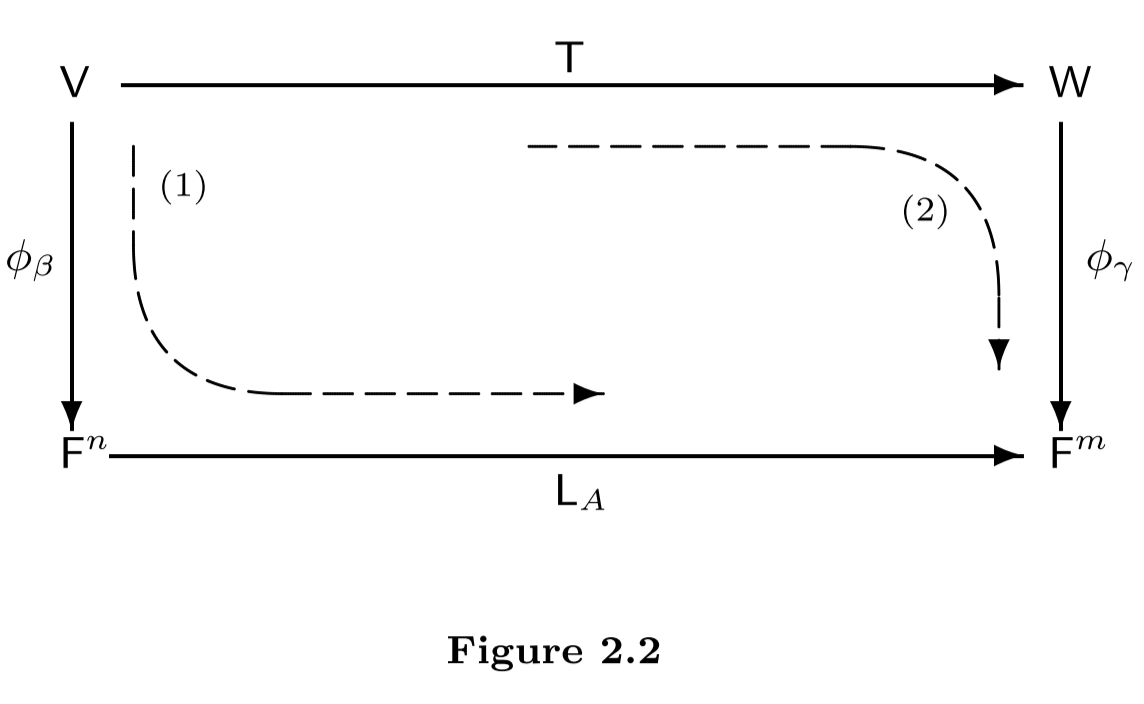
\includegraphics[width=16cm]{images/figure-2-2.png}

Let us first consider Figure 2.2.
Notice that there are two \emph{composites} of \LTRAN{}s that map \(\V\) into \(F^m\):
\begin{enumerate}
\item[1.] Map \(\V\) into \(F^n\) with \(\phi_{\beta}\) and follow this transformation with \(\LMTRAN_A\);
    this yields the composite \(\LMTRAN_A \phi_{\beta}\).
\item[2.] Map \(\V\) into \(\W\) with \(\T\) and follow it by \(\phi_{\gamma}\) to obtain the composite \(\phi_{\gamma} \T\).
\end{enumerate}

\begin{remark} \label{remark 2.4.6}
These two composites are depicted by the dashed arrows in the diagram.
By a simple reformulation of \THM{2.14}, we may conclude that for all \(v \in \V\),
\begin{align*}
    \LMTRAN_A \phi_{\beta}(v)
    & = \LMTRAN_A (\phi_{\beta}(v)) & \text{by def of composition} \\
    & = \LMTRAN_A([v]_{\beta}) & \text{by def of \(\phi_{\beta}\)} \\
    & = A [v]_{\beta} & \text{by def of \(\LMTRAN_A\)} \\
    & = [\T]_{\beta}^{\gamma} [v]_{\beta} & \text{since \(A = [\T]_{\beta}^{\gamma}\)} \\
    & = [\T(v)]_{\gamma} & \text{by \THM{2.14}} \\
    & = \phi_{\gamma}(\T(v)) & \text{by def of \(\phi_{\gamma}\)} \\
    & = \phi_{\gamma} \T (v), & \text{by def of composition}
\end{align*}

Hence \(\LMTRAN_A \phi_{\beta} = \phi_{\gamma} \T\);
that is. the diagram ``commutes.'' (It seems that the terminology is from abstract algebra.)

Heuristically, this relationship indicates that after \(\V\) and \(\W\) are \emph{identified} with \(F^n\) and \(F^m\) via if \(\phi_{\beta}\) and \(\phi_{\gamma}\), respectively,
we may ``identify'' \(\T\) with \(\LMTRAN_A\).
\textbf{This diagram allows us to transfer operations on abstract vector spaces to ones on \(F^n\) and \(F^m\)}.
\end{remark}

\begin{example} \label{example 2.4.7}
Recall the \LTRAN{} \(\T : \POLYRRR \to \POLYRR\) defined in \EXAMPLE{2.2.4} (\(\T(f(x)) = f'(x)\)).
Let \(\beta\) and \(\gamma\) be the standard ordered bases for \(\POLYRRR\) and \(\POLYRR\), respectively,
and let \(\phi_{\beta} : \POLYRRR \to \SET{R}^4\) and \(\phi_{\gamma} : \POLYRR \to \SET{R}^3\) be the corresponding standard representations of \(\POLYRRR\) and \(\POLYRR\).
If \(A = [\T]_{\beta}^{\gamma}\), then
\[
    A = \begin{pmatrix} 0 & 1 & 0 & 0 \\ 0 & 0 & 2 & 0 \\ 0 & 0 & 0 & 3 \end{pmatrix}
\]
Consider the polynomial \(p(x) = 2 + x - 3x^2 + 5x^3\).
We show that \(\LMTRAN_A \phi_{\beta} (p(x)) = \phi_{\gamma} \T (p(x))\).
Now
\[
    \LMTRAN_A \phi_{\beta} (p(x)) = [A]_{\beta}^{\gamma} [p(x)]_{\beta} 
    = \begin{pmatrix} 0 & 1 & 0 & 0 \\ 0 & 0 & 2 & 0 \\ 0 & 0 & 0 & 3 \end{pmatrix} \begin{pmatrix} 2 \\ 1 \\ -3 \\ 5 \end{pmatrix} = \begin{pmatrix} 1 \\ -6 \\ 15 \end{pmatrix}
\]
And since \(\T(p(x)) = p'(x) = 1 - 6x + 15x^2\), we have
\[
    \phi_{\gamma} \T (p(x)) = \phi_{\gamma} (1 - 6x + 15 x^2) = \begin{pmatrix} 1 \\ -6 \\ 15 \end{pmatrix}
\]
So \(\LMTRAN_A \phi_{\beta} (p(x)) = \phi_{\gamma} \T (p(x))\).
\end{example}

\exercisesection

\begin{exercise} \label{exercise 2.4.1}
Label the following statements as true or false.
In each part, \(V\) and \(W\) are vector spaces with ordered (finite) bases \(\alpha\) and \(\beta\), respectively, \(\T: V \to W\) is linear, and \(A\) and \(B\) are matrices.
\begin{enumerate}
\item \(([\T]_{\alpha}^{\beta})^{-1} = [\T^{-1}]_{\alpha}^{\beta}\).
\item \(\T\) is invertible if and only if \(\T\) is one-to-one and onto.
\item \(\T = \LMTRAN_A\), where \(A = [\T]_{\alpha}^{\beta}\).
\item \(M_{2 \X 3}(F)\) is isomorphic to \(F^5\).
\item \(\POLYNF\) is isomorphic to \(\mathcal{P}_m(F)\) if and only if \(n = m\).
\item \(AB = I\) implies that \(A\) and \(B\) are invertible.
\item If \(A\) is invertible, then \((A^{-1})^{-1} = A\).
\item \(A\) is invertible if and only if \(\LMTRAN_A\) is invertible.
\item \(A\) must be square in order to possess an inverse.
\end{enumerate}
\end{exercise}

\begin{proof} \ 

\begin{enumerate}
\item False.
    First, \(\T\) should be invertible to make \(\T^{-1}\) and \(([\T]_{\alpha}^{\beta})^{-1}\) well defined.
    Second, if \(\T\) is invertible, then by \THM{2.18}, \(([\T]_{\alpha}^{\beta})^{-1} = [\T^{-1}]_{\beta}^{\alpha}\).
\item True, this is just true for normal functions.
\item False. the domain and codomain of \(\T\) and \(\LMTRAN_A\) are not necessarily the same.
\item False, \(\dim(M_{2 \X 3}(F)) = 6 \ne 5 = \dim(F^5)\), so by \THM{2.19}, they are not isomorphic to each other.
\item True, \(\POLYNF\) is isomorphic to \(\mathcal{P}_m(F)\), if and only if (by \THM{2.19}) their dimension are equal, that is, if and only if \(n = m\).
\item False, by \DEF{2.13} we also need to check \(BA = I\); and \(A, B\) \emph{must be squares of the same size}.
    Counter example:
    \[
        \left(\begin{array}{lll}
            1 & 0 & 0 \\
            0 & 1 & 0
        \end{array}\right)
        \left(\begin{array}{ll}
            1 & 0 \\
            0 & 1 \\
            0 & 0
        \end{array}\right) = I_2
    \]
\item True.
    If \(A\) is invertible, then by \DEF{2.13}(3) we denote its inverse as \(A^{-1}\);
    in particular by \DEF{2.13}(1) we have \(A A^{-1} = A^{-1} A = I\).
    But this immediately implies \(A^{-1} A = A A^{-1} = I\), so by \DEF{2.13}(1) again, the (unique) inverse of \(A^{-1}\) is \(A\), that is, \((A^{-1})^{-1} = A\).
\item True by \CORO{2.18.2}.
\item True, by \DEF{2.13} (We only define ``invertible'' on square matrix'').
\end{enumerate}
\end{proof}

\begin{exercise} \label{exercise 2.4.2}
For each of the following linear transformations \(\T\), determine whether \(\T\) is invertible and justify your answer.
\begin{enumerate}
\item \(\T : \SET{R}^2 \to \SET{R}^3\) defined by \(\T(a_1, a_2) = (a_1 - 2a_2, a_2, 3a_1 + 4a_2)\).
\item \(\T : \SET{R}^2 \to \SET{R}^3\) defined by \(\T(a_1, a_2) = (3a_1 - a_2, a_2, 4a_1)\).
\item \(\T : \SET{R}^3 \to \SET{R}^3\) defined by \(\T(a_1, a_2, a_3) = (3a_1 - 2a_3, a_2, 3a_1 + 4a_2)\).
\item \(\T : \POLYRRR \to \POLYRR\) defined by \(\T(p(x)) = p'(x)\).
\item \(\T: M_{2 \X 2}(\SET{R}) \to \POLYRR\) defined by \(\T \begin{pmatrix} a & b \\ c & d \end{pmatrix} = a + 2bx + (c + d)x^2\).
\item \(\T : M_{2 \X 2}(\SET{R}) \to M_{2 \X 2}(\SET{R})\) defined by \(\T \begin{pmatrix} a & b \\ c & d \end{pmatrix} = \begin{pmatrix} a + b & a \\ c & c + d \end{pmatrix}\).
\end{enumerate}
\end{exercise}

\begin{proof} \ 

\begin{enumerate}
\item \(\T\) is not invertible since it cannot be an isomorphism by \THM{2.19}.
\item \(\T\) is not invertible since it cannot be an isomorphism by \THM{2.19}.
\item True.
    It's easy to check \(\NULLT = \{ (0, 0, 0) \}\), hence (by \THM{2.4}) \(\T\) is one-to-one (and by \THM{2.5}) is onto;
    and of course \(\T\) is linear, hence (by \RMK{2.4.1}) is invertible.
\item \(\T\) is not invertible since it cannot be an isomorphism by \THM{2.19}.
\item \(\T\) is not invertible since it cannot be an isomorphism by \THM{2.19}.
\item \(\T\) is invertible;
    It's easy to check \(\NULLT = \bigg\{ \begin{pmatrix} 0 & 0 \\ 0 & 0 \end{pmatrix} \bigg\}\), hence \(\T\) is one-to-one, and onto by \THM{2.5};
    and of course \(\T\) is linear.
\end{enumerate}
\end{proof}

\begin{exercise} \label{exercise 2.4.3}
Which of the following pairs of vector spaces are isomorphic?
Justify your answers.
\begin{enumerate}
\item \(F^3\) and \(\mathcal{P}_3(F)\).
\item \(F^4\) and \(\mathcal{P}_3(F)\).
\item \(M_{2 \X 2}(\SET{R})\) and \(\POLYRRR\).
\item \(V = \{ A \in M_{2 \X 2}(\SET{R}) : \TRACE(A) = 0 \}\) and \(\SET{R}^4\).
\end{enumerate}
\end{exercise}

\begin{proof} \ 
\begin{enumerate}
\item \(\dim(F^3) = 3\), \(\dim(\mathcal{P}_3(F)) = 4\), so \(F^3\) and \(\mathcal{P}_3(F)\) are not isomorphic by \THM{2.19}.
\item \(\dim(F^4) = 4\), \(\dim(\mathcal{P}_3(F)) = 4\), so \(F^4\) and \(\mathcal{P}_3(F)\) are isomorphic by \THM{2.19}.
\item \(\dim(M_{2 \X 2}(\SET{R})) = 4\), \(\dim(\mathcal{P}_3(F)) = 4\), so \(M_{2 \X 2}(\SET{R})\) and \(\mathcal{P}_3(F)\) are isomorphic by \THM{2.19}.
\item \(\dim(V) = 2^2 - 1 = 3\) by \ATHM{1.19}(1), \(\dim(\SET{R}^4) = 4\), so \(V\) and \(\SET{R}^4\) are not isomorphic by \THM{2.19}.
\end{enumerate}
\end{proof}

\begin{exercise} \label{exercise 2.4.4}
Let \(A\) and \(B\) be \(n \X n\) invertible matrices.
Prove that \(AB\) is invertible and \((AB)^{-1} = B^{-1}A^{-1}\).
\end{exercise}

\begin{proof}
We have
\begin{align*}
    (AB)(B^{-1}A^{-1}) & = ( A(B B^{-1}) )A^{-1} & \text{by \THM{2.16}, associative} \\
                       & = (A I_n) A^{-1} \\
                       & = A A^{-1} & \text{by \THM{2.12}(c)} \\
                       & = I_n,
\end{align*}
and
\begin{align*}
    (B^{-1}A^{-1})(AB) & = ( B(A A^{-1}) )B^{-1} & \text{by \THM{2.16}, associative} \\
                       & = (B I_n) B^{-1} \\
                       & = B B^{-1} & \text{by \THM{2.12}(c)} \\
                       & = I_n,
\end{align*}
so by \DEF{2.13}, \(AB\) is invertible, and (since the inverse is unique,) \((AB)^{-1} = B^{-1} A^{-1}\).
\end{proof}

\begin{exercise} \label{exercise 2.4.5}
Let \(A\) be invertible.
Prove that \(A^\top\) is invertible and \((A^\top)^{-1} = (A^{-1})^\top\).
\end{exercise}

\begin{note}
The inverse of the transpose of \(A\) is equal to the transpose of the inverse of \(A\), when \(A\) is invertible.
\end{note}

\begin{proof}
We have
\begin{align*}
    A^\top (A^{-1})^\top & = ( A^{-1} A )^\top & \text{by \ATHM{2.24}} \\
                       & = I_n^\top \\
                       & = I_n, & \text{of course}
\end{align*}
and
\begin{align*}
    (A^{-1})^\top A^\top  & = ( A A^{-1} )^\top & \text{by \ATHM{2.24}} \\
                       & = I_n^\top \\
                       & = I_n, & \text{of course}
\end{align*}
so by \DEF{2.13}, \(A^\top\) is invertible, and (since the inverse is unique,) \((A^\top)^{-1} = (A^{-1})^\top\).
\end{proof}

\begin{exercise} \label{exercise 2.4.6}
Prove that if \(A\) is \textbf{invertible} and \(AB = O\), then \(B = O\).
\end{exercise}

\begin{proof}
We have
\begin{align*}
             & AB = O \\
    \implies & A^{-1}(AB) = A^{-1} O = O \\
    \implies & (A^{-1} A)B = O & \text{by \THM{2.16}, associative} \\
    \implies & IB = O \\
    \implies & B = O. & \text{by \THM{2.12}(c)}
\end{align*}
\end{proof}

\begin{exercise} \label{exercise 2.4.7}
Let \(A\) be an \(n \X n\) matrix.
\begin{enumerate}
\item Suppose that \(A^2 = O_{n \X n}\).
    Prove that \(A\) is not invertible.
\item Suppose that \(AB = O_{n \X n}\) for some \textbf{nonzero} \(n \X n\) matrix \(B\).
    Could \(A\) be invertible? Explain.
\end{enumerate}
\end{exercise}

\begin{proof} \ 
\begin{enumerate}
\item For the sake of contradiction, suppose \(A\) is invertible (so we have \(A^{-1}\)).
Then
\begin{align*}
             & A^2 = O_{n \X n} \\
    \implies & A^{-1} (A^2) = A^{-1} O_{n \X n} = O_{n \X n} \\
    \implies & (A^{-1} A) A = O_{n \X n} & \text{by \THM{2.16}, associative} \\
    \implies & IA = O_{n \X n} \\
    \implies & A = O_{n \X n}, & \text{by \THM{2.13}(c)}
\end{align*}
which implies \(A\) is equal to a matrix that is not invertible, a contradiction.
Hence \(A\) is not invertible.

\item
If \(A\) is invertible, then
\begin{align*}
             & AB = O_{n \X n} \\
    \implies & A^{-1} (AB) = A O_{n \X n} = O_{n \X n} \\
    \implies & (A^{-1} A)B = O_{n \X n} & \text{by \THM{2.16}, associative} \\
    \implies & IB = O_{n \X n} \\
    \implies & B = O_{n \X n}, & \text{by \THM{2.13}(c)}
\end{align*}
which contradicts that \(B\) is nonzero.
Hence \(A\) is not invertible.
\end{enumerate}
\end{proof}

\begin{exercise} \label{exercise 2.4.8}
Prove \CORO{2.18.1} and \CORO{2.18.2}.
\end{exercise}

\begin{proof}
See \CORO{2.18.1} and \CORO{2.18.2}.
\end{proof}

\begin{exercise} \label{exercise 2.4.9}
Let \(A\) and \(B\) be \(n \X n\) matrices such that \(AB\) is invertible.
\begin{enumerate}
\item Prove that (\textbf{both}) \(A\) and \(B\) are invertible.
    Hint: See \ATHM{2.26}.
\item Give an example to show that a product of \emph{nonsquare} matrices can be invertible even though the factors, by definition, are not.
\end{enumerate}
\end{exercise}

\begin{note}
By part(b), the supposition that both \(A\) and \(B\) are \(n \X n\) matrix are essential to conclude that they are invertible.
\end{note}

\begin{proof}
Let \(\beta\) be the standard ordered basis for \(F^n\).
Then by \THM{2.15}(a), \([\LMTRAN_A]_{\beta} = A\), \([\LMTRAN_B]_{\beta} = B\), \([\LMTRAN_{AB}]_{\beta} = AB\),
and of course \(\LMTRAN_A, \LMTRAN_B, \LMTRAN_{AB}\) are linear.
\begin{enumerate}
\item Since \(AB\) is invertible, that is, \([\LMTRAN_{AB}]_{\beta}\) is invertible, by \THM{2.18}, \(\LMTRAN_{AB}\) is invertible, that is, by \THM{2.15}(e), \(\LMTRAN_A \LMTRAN_B\) is invertible.
By \ATHM{2.26}(1), \(\LMTRAN_B\) is one-to-one, and by \THM{2.5} (since domain/codomain have the same \(\dim\)), \(\LMTRAN_B\) is onto,
hence \(\LMTRAN_B\) is invertible, hence by \THM{2.18}, \([\LMTRAN_B]_{\beta}\) is invertible, that is, \(B\) is invertible.
Similarly, by \ATHM{2.26}(2), \(\LMTRAN_A\) is onto, and by \THM{2.5} (since domain/codomain have the same \(\dim\)), \(\LMTRAN_A\) is one-to-one,
hence \(\LMTRAN_A\) is invertible, hence by \THM{2.18}, \([\LMTRAN_A]_{\beta}\) is invertible, that is, \(A\) is invertible.

\item
We have
\begin{align*}
    \begin{pmatrix} 1 & 2 & 3 \end{pmatrix}
    \begin{pmatrix} 1 \\ 2 \\ 3 \end{pmatrix}
    = \begin{pmatrix} 10 \end{pmatrix},
\end{align*}
which is an \(1 \X 1\) matrix and has inverse \(( \frac{1}{10} )\).
\end{enumerate}
\end{proof}

\begin{exercise} \label{exercise 2.4.10}
Let \(A\) and \(B\) be \(n \X n\) matrices such that \(AB = I_n\).
\begin{enumerate}
\item Use \EXEC{2.4.9} to conclude that (\textbf{both}) \(A\) and \(B\) are invertible.
\item Prove \(A = B^{-1}\) (and hence \(B = A^{-1}\)).
    (We are, in effect, \textbf{saying that for square matrices, a "one-sided" inverse is a "two-sided" inverse.})
\item State and prove analogous results for linear transformations defined on finite-dimensional vector spaces.
\end{enumerate}
\end{exercise}

\begin{note}
Part(b) says, if \(A, B\) are squares and \(AB = I_n\), then we automatically have \(BA = I_n\), and \(A, B\) are inverse matrices of each other.
\end{note}

\begin{proof} \ 
\begin{enumerate}
\item If \(AB = I_n\), that simply means \(AB\) is invertible, since \(I_n\) is invertible.
So the conditions of \EXEC{2.4.9}(a) are satisfied, hence both \(A, B\) are invertible.

\item We have
\begin{align*}
             & AB = I_n \\
    \implies & A^{-1} (AB) = A^{-1} I_n = A^{-1} & \text{since \(A\) is invertible, and by \THM{2.12}(c)} \\
    \implies & (A^{-1}A)B = A^{-1} & \text{by \THM{2.16}, associative} \\
    \implies & I_n B = A^{-1} \\
    \implies & B = A^{-1}. & \text{by \THM{2.12}(c)}
\end{align*}
And by \DEF{2.13}, this implies \(AB = BA = I_n\).
In particular, we have \(BA = AB = I_n\), so by \DEF{2.13} again, \(B^{-1} = A\).

\item
Statement: Let \(\T : V \to W\) and \(\U : W \to V\) where \(V, W\) have same (finite) dimensions and \(\U\T = \ITRANV\).
Then both \(\U, \T\) are invertible. and we have \((\T)^{-1} = \U\) (hence \(\U^{-1} = \T\)).

First, similar to \EXEC{2.4.9}, by \ATHM{2.26}(1)(2), both \(\U, \T\) are invertible.
And (by general version of \THM{2.10},) we have
\begin{align*}
             & \U\T = \ITRANV \\
    \implies & \U^{-1} (\U\T) = \U^{-1} \ITRANV = \U^{-1} & \text{since \(\U\) is invertible, and by \THM{2.10}(c)} \\
    \implies & (\U^{-1}\U)\T = \U^{-1} & \text{by \THM{2.10}(b), associative} \\
    \implies & \ITRANW \T = \U^{-1} \\
    \implies & \T = \U^{-1}. & \text{by \THM{2.10}(c)}
\end{align*}
And by \DEF{2.12}, this implies \(\U\T = \ITRANV\) and \(\T\U = \ITRANW\).
In particular, we have \(\T\U = \ITRANW\) and \(\U\T = \ITRANV\) and, so by \DEF{2.12} again, \(\T^{-1} = \U\).
\end{enumerate}
\end{proof}

\begin{exercise} \label{exercise 2.4.11}
Verify that the transformation in \EXAMPLE{2.4.5} is one-to-one.
\end{exercise}

\begin{proof}
Suppose \(f \in \NULLT\), we have to show \(f\) is zero polynomial to show \(\T\) is one-to-one.
Then we have \(f(1) = f(2) = f(3) = f(4) = 0\).
But by \RMK{1.6.6} we know that \(f\) is the zero polynomial, as desired.
\end{proof}

\begin{exercise} \label{exercise 2.4.12}
Prove \THM{2.21}.
\end{exercise}

\begin{proof}
See \THM{2.21}.
\end{proof}

\begin{exercise} \label{exercise 2.4.13}
Let \(\sim\) mean ``is isomorphic to.'' (\DEF{2.14})
Prove that \(\sim\) is an equivalence relation on the class of vector spaces over \(F\).
\end{exercise}

\begin{proof}\ 

Reflexivity: \(V\) is isomorphic to \(V\) since \(\ITRANV\) is an isomorphism from \(V\) to \(V\) for any vector space \(V\).

Symmetry: Suppose \(V\) is isomorphic to \(W\), then there exists an isomorphism \(\T\) from \(V\) to \(W\).
In particular, by \DEF{2.14}, \(\T\) is invertible, so \(\T^{-1} : W \to V\) exists, and also invertible.
And by \THM{2.17}, \(\T^{-1}\) is linear.
Hence by \DEF{2.14} again, \(\T^{-1}\) is an isomorphism from \(W\) to \(V\).
Hence \(W\) is isomorphic to \(V\).

Transitivity: Suppose \(V\) is isomorphic to \(W\) and \(W\) is isomorphic to \(Z\), then there exists an isomorphism \(\T\) from \(V\) to \(W\) and \(\U\) from \(W\) to \(Z\).
Furthermore, by \ATHM{2.26}(c) \(\U\T\) is invertible, and by \THM{2.9}, since \(\U, \T\) are linear, \(\U\T\) is also linear, hence \(\U\T\) is an isomorphism by \DEF{2.14}.
Hence \(V\) is isomorphic to \(Z\).
\end{proof}

\begin{exercise} \label{exercise 2.4.14}
Let
\[
    V = \bigg\{ \begin{pmatrix} a & a + b \\ 0 & c \end{pmatrix} : a, b, c \in F \bigg\}.
\]
Construct an isomorphism from \(V\) to \(F^3\).
\end{exercise}

\begin{proof}
Clearly,
\[\beta = \bigg\{
    \begin{pmatrix} 1 & 0 \\ 0 & 0 \end{pmatrix},
    \begin{pmatrix} 0 & 1 \\ 0 & 0 \end{pmatrix},
    \begin{pmatrix} 0 & 0 \\ 0 & 1 \end{pmatrix}
\bigg\}\]
is a basis for \(V\).
Then by \THM{2.21}, \(\phi_{\beta}\) is an isomorphism from \(V\) to \(F^3\).
\end{proof}

\begin{exercise} \label{exercise 2.4.15}
Let \(V\) and \(W\) be \(n\)-dimensional vector spaces, and let \(\T : V \to W\) be a linear transformation.
Suppose that \(\beta\) is a basis for \(V\).
Prove that \(\T\) is an isomorphism \emph{if and only if} \(\T(\beta)\) is a basis for \(W\).
\end{exercise}

\begin{proof} \ 

\(\Longrightarrow\): Suppose \(\T\) is an isomorphism.
In particular, \(\T\) is one-to-one and onto.
Then by \ATHM{2.2}(2.c), \(\T(\beta)\) is a basis for \(W\).

\(\Longleftarrow\): Suppose \(\T(\beta)\) is a basis for \(W\).
In particular, \(\spann(\T(\beta)) = W\).
And by \THM{2.2}, \(\RANGET = \spann(\T(\beta)) = W\), hence \(\T\) is onto.
By \THM{2.5}, \(\T\) is one-to-one.
Hence \(\T\) is an isomorphism.
\end{proof}

\begin{exercise} \label{exercise 2.4.16}
Let \(B\) be an \(n \X n\) \emph{invertible} matrix.
Define \(\Phi : M_{n \X n}(F) \to M_{n \X n}(F)\) by \(\Phi(A) = B^{-1}AB\).
Prove that \(\Phi\) is an isomorphism.
\end{exercise}

\begin{note}
This is called ``matrix similarity''; we say that \(\Phi(A)\)(or \(B^{-1}AB\)) and \(A\) are similar.
This concept is introduced in the next section(\DEF{2.16}) and is used in \CH{5}.
\end{note}

\begin{proof}
First, it's trivial that \(\Phi\) is linear since it only involves matrix multiplication and you can use \THM{2.10} to check linearity.
Now to show that \(\Phi\) is invertible, since domain/codomain have the same dimensions, we only need to show \(\Phi\) is onto.
But given \(D \in M_{n \X n}(F)\), we have \(B D B^{-1} \in M_{n \X n}(F)\) such that
\begin{align*}
    \Phi(B D B^{-1}) & = B^{-1} (B D B^{-1}) B & \text{by def of \(\Phi\)} \\
                     & = (B^{-1}B) D (B^{-1} B) & \text{of course} \\
                     & = IDI & \text{of course} \\
                     & = D & \text{of course}
\end{align*}
So \(\Phi\) is onto, as desired.
\end{proof}

\begin{exercise} \label{exercise 2.4.17}
Let \(V\) and \(W\) be finite-dimensional vector spaces and \(\T : V \to W\) be an isomorphism.
Let \(V_0\) be a \emph{subspace} of \(V\).
\begin{enumerate}
\item Prove that \(\T(V_0)\) is a subspace of \(W\).
\item Prove that \(\dim(V_0) = \dim(\T(V_0))\).
\end{enumerate}
And from part(b), we say that an isomorphism is \emph{rank-preserving}, since in particular \(\dim(V) = \dim(\T(V))\).
\end{exercise}

\begin{proof} \ 

\begin{enumerate}
\item It is true by \ATHM{2.4}(1).
\item By \THM{2.19}, it suffices to show that \(V_0\) and \(\T(V_0)\) are isomorphic.
And we claim that \(\T' : V_0 \to \T(V_0)\) by \(\T'(v) = \T(v)\) for \(v \in V_0\) is an isomorphism from \(V_0\) to \(\T(V_0)\).

First, of course \(\T'\) is linear.
For one-to-one, given \(v_1, v_2 \in V_0\),
\begin{align*}
             & \T'(v_1) = \T'(v_2) \\
    \implies & \T(v_1) = \T(v_2) & \text{by def of \(\T'\)} \\
    \implies & v_1 = v_2. & \text{since in particular \(\T\) is one-to-one}
\end{align*}

For onto, given \(w \in \T(V_0)\), then by definition of \(\T(V_0)\) we of course can find \(v \in V_0\) such that \(\T(v) = W\).
But since \(v \in V_0\), \(\T'(v) = \T(v)\).
Hence we have found \(v \in V_0\) such that \(\T'(v) = w\), so \(\T'\) is onto.

So \(\T'\) is an isomorphism from \(V_0\) to \(\T(V_0)\), as desired.
\end{enumerate}

\end{proof}

\begin{exercise} \label{exercise 2.4.18}
Repeat \EXAMPLE{2.4.7} with the polynomial \(p(x) = 1 + x + 2x^2 + x^3\).
\end{exercise}

\begin{proof}
Let 
\[
    A = [\T]_{\beta}^{\gamma} = \begin{pmatrix} 0 & 1 & 0 & 0 \\ 0 & 0 & 2 & 0 \\ 0 & 0 & 0 & 3 \end{pmatrix}
\]
We show that \(\LMTRAN_A \phi_{\beta} (p(x)) = \phi_{\gamma} \T (p(x))\).
Now
\[
    \LMTRAN_A \phi_{\beta} (p(x)) = [A]_{\beta}^{\gamma} [p(x)]_{\beta} 
    = \begin{pmatrix} 0 & 1 & 0 & 0 \\ 0 & 0 & 2 & 0 \\ 0 & 0 & 0 & 3 \end{pmatrix} \begin{pmatrix} 1 \\ 1 \\ 2 \\ 1 \end{pmatrix} = \begin{pmatrix} 1 \\ 4 \\ 3 \end{pmatrix}
\]
But since \(\T(p(x)) = p'(x) = 1 + 4x + 3x^2\), we have
\[
    \phi_{\gamma} \T (p(x)) = \phi_{\gamma} (1 + 4x + 3x^2) = \begin{pmatrix} 1 \\ 4 \\ 3 \end{pmatrix}
\]
So \(\LMTRAN_A \phi_{\beta} (p(x)) = \phi_{\gamma} \T (p(x))\).
\end{proof}

\begin{exercise} \label{exercise 2.4.19}
In \EXAMPLE{2.1.5}, the mapping \(\T : M_{2 \X 2}(\SET{R}) \to M_{2 \X 2}(\SET{R})\) defined by \(\T(M) = M^\top\) for each \(M \in M_{2 \X 2}(\SET{R})\) is a linear transformation.
Let \(\beta = \{ E_{11}, E_{12}, E_{21}, E_{22} \}\), which is a basis for \(M_{2 \X 2}(\SET{R})\), as noted in \EXAMPLE{1.6.3}.
\begin{enumerate}
\item Compute \([\T]_{\beta}\).
\item Verify that \(\LMTRAN_A \phi_{\beta} (M) = \phi_{\beta} \T(M)\) for \(A = [\T]_{\beta}\) and \(M = \begin{pmatrix} 1 & 2 \\ 3 & 4 \end{pmatrix}\).
\end{enumerate}
\end{exercise}

\begin{proof} \ 

\begin{enumerate}
\item From \EXEC{2.2.5}(a),
\[
    [\T]_{\beta}
    = \begin{pmatrix}
        \MAROON{1} & \BLUE{0} & \RED{0} & \GREEN{0} \\
        \MAROON{0} & \BLUE{0} & \RED{1} & \GREEN{0} \\
        \MAROON{0} & \BLUE{1} & \RED{0} & \GREEN{0} \\
        \MAROON{0} & \BLUE{0} & \RED{0} & \GREEN{1}
    \end{pmatrix}
\]

\item
\[
    \LMTRAN_A \phi_{\beta}(M) = 
    = \begin{pmatrix}
        1 & 0 & 0 & 0 \\
        0 & 0 & 1 & 0 \\
        0 & 1 & 0 & 1 \\
        0 & 0 & 0 & 1
    \end{pmatrix}
    \begin{pmatrix} 1 \\ 2 \\ 3 \\4 \end{pmatrix}
    = \begin{pmatrix} 1 \\ 3 \\ 2 \\ 4 \end{pmatrix}
\]
and
\[
    \phi_{\beta}\T(M)
    = \phi_{\beta}\begin{pmatrix} 1 & 3 \\ 2 & 4 \end{pmatrix}
    = \begin{pmatrix} 1 \\ 3 \\ 2 \\ 4 \end{pmatrix}
\]
So \(\LMTRAN_A \phi_{\beta}(M) = \phi_{\beta}\T(M)\).
\end{enumerate}
\end{proof}

\begin{exercise} \label{exercise 2.4.20}
Let \(\T: V \to W\) be a \LTRAN{} from an \(n\)-dimensional vector space \(V\) to an \(m\)-dimensional vector space \(W\).
Let \(\beta\) and \(\gamma\) be ordered bases for \(V\) and \(W\), respectively.
Prove that \(\rankT = \rank(\LMTRAN_A)\) and that \(\nullityT = \nullity(\LMTRAN_A)\), where \(A = [\T]_{\beta}^{\gamma}\).
Hint: Apply \EXEC{2.4.17} to Figure 2.2.
\end{exercise}

\begin{proof} \ 

\(\rankT = \rank(\LMTRAN_A)\):
Since \(\LMTRAN_A \phi_{\beta} = \phi_{\gamma} \T \), in particular we have \(\LMTRAN_A \phi_{\beta}(V) = \phi_{\gamma} \T(V)\) \MAROON{(1)}.

Now, for the dimension of RHS of \MAROON{(1)},
\begin{align*}
    & \dim(\phi_{\gamma} \T(V)) \\
    & = \dim(\phi_{\gamma} (\T(V))) & \text{by def of composition} \\
    & = \dim(\T(V)) & \text{since \(\phi_{\gamma}\) is an isomorphism, and by \EXEC{2.4.17}(b)} \\
    & = \rankT, & \text{by definition}
\end{align*}
and for the dimension of LHS of \MAROON{(1)},
\begin{align*}
    & \dim(\LMTRAN_A \phi_{\beta}(V)) \\
    & = \dim(\LMTRAN_A (\phi_{\beta}(V))) & \text{by def of composition} \\
    & = \dim(\LMTRAN_A (F^n)) & \text{since (in particular) \(\phi_{\beta}\) is onto} \\
    & = \dim(\RANGE(\LMTRAN_A)) & \text{by definition} \\
    & = \rank(\LMTRAN_A), & \text{by definition}
\end{align*}
Hence we have \(\rankT = \rank(\LMTRAN_A)\), as desired.

\(\nullityT = \nullity(\LMTRAN_A)\):
We have
\begin{align*}
    \nullityT & = \dim(V) - \rankT & \text{by \THM{2.3}(dimension theorem)} \\
              & = \dim(F^n) - \rankT & \text{of course, since \(\dim(V) = n\)} \\
              & = \dim(F^n) - \rank(\LMTRAN_A) & \text{by what we have shown} \\
              & = \nullity(\LMTRAN_A). & \text{again by \THM{2.3}}
\end{align*}
\end{proof}

\begin{exercise} \label{exercise 2.4.21}
Let \(V\) and \(W\) be \emph{finite}-dimensional vector spaces with ordered bases \(\beta = \{ v_1, v_2, ..., v_n \}\) and \(\gamma = \{ w_1, w_2, ..., w_m \}\), respectively.
By \THM{2.6}, there exist unique linear transformations \(\T_{ij} : V \to W\) such that
\begin{equation*}
    \T_{ij}(v_k) = \begin{cases}
        w_i, \text{ if } k = j \\
        \OW, \text{ if } k \ne j
    \end{cases}
\end{equation*}
First prove that \(\alpha = \{ T_{ij} : 1 \le i \le m, 1 \le j \le n \}\) is a basis for \(\mathcal{L}(V, W)\).
Then let \(M^{ij}\) be the \(m \X n\) matrix with \(1\) in the \(i\)th row and \(j\)th column and \(0\) elsewhere, and prove that \([\T_{ij}]_{\beta}^{\gamma} = M^{ij}\).
Again by \THM{2.6}, there exists a unique linear transformation \(\Phi_{\beta}^{\gamma} : \mathcal{L}(V, W) \to M_{m \X n}(F)\) such that \(\Phi_{\beta}^{\gamma} (\T_{ij}) = M^{ij}\).
Prove that \(\Phi_{\beta}^{\gamma}\) is an isomorphism.
\end{exercise}

\begin{proof}
Since \(\#\alpha = \dim(\mathcal{L}(V, W)\) (where by \THM{2.20} we can conclude \(\dim(\mathcal{L}(V, W) = mn\)), (by \CORO{1.10.3}(b)) we only need to show \(\alpha\) is \LID{}.
BTW, we use the symbol \(\TZERO\) to represent the zero vector, i.e. the zero transformation, of \(\mathcal{L}(V, W)\).

So suppose \(\sum_{i = 1}^{m} \sum_{j = 1}^n a_{ij} \T_{ij} = \TZERO\) \MAROON{(1)}, we have to show \(a_{ij} = 0\) for all \(1 \le i \le m\), \(1 \le j \le n\).
But given arbitrary \(k\) such that \(1 \le k \le n\),
\begin{align*}
    \OW & = \TZERO(v_k) & \text{of course} \\
        & = \bigg( \sum_{i = 1}^{m} \sum_{j = 1}^n a_{ij} \T_{ij} \bigg) (v_k) & \text{by \MAROON{(1)}} \\
        & = \sum_{i = 1}^{m} \sum_{j = 1}^n a_{ij} \T_{ij} (v_k) & \text{by def of \(+\) and scalar \(\cdot\) of functions} \\
        & = \sum_{i = 1}^{m} \bigg( a_{i1} \T_{i1} (v_k) + a_{i2} \T_{i2} (v_k) + ... + a_{in} \T_{in} (v_k) \bigg) & \text{expanding summation} \\
        & = \sum_{i = 1}^{m} \bigg( a_{i1} \OV + ... + a_{ik} w_i + ... + a_{in} \OV \bigg) & \text{by definition of \(\T_{ij}\)} \\
        & = \sum_{i = 1}^m a_{ik} w_i,
\end{align*}
which implies \(a_{1k} = a_{2k} = ... = a_{mk} = 0\) since \(\gamma\) is a basis for \(W\).
Since \(k\) is arbitrary, we have \(a_{ik} = 1\) for all \(1 \le i \le m\), \(1 \le k \le n\), as desired.

Now given arbitrary \(j\) such that \(1 \le j \le n\), it trivial that the \(j\)th column of \(M^{ij}\) is \(e_i\) where \(e_i\) is the \(i\)th standard vector of \(F^m\).
And by definition, the \(j\)th column of \([\T_{ij}]_{\beta}^{\gamma}\) is \([\T_{ij}(v_j)]_{\gamma}\), but
\begin{align*}
    [\T_{ij}(v_j)]_{\gamma} & = [w_i]_{\gamma} & \text{by definition of \(T^{ij}\)} \\
                 & = e_i & \text{of course}
\end{align*}
Hence \(M^{ij} = [\T_{ij}]_{\gamma}\).

Finally, And since \(\alpha' = \{ M_{ij} : 1 \le i \le m, 1 \le j \le n \}\) is a basis for \(M_{m \X n}(F)\), and \(\Phi_{\beta}^{\gamma}(\alpha) = \alpha'\), by \EXEC{2.4.15}, \(\Phi_{\beta}^{\gamma}\) is an isomorphism.
\end{proof}

\begin{exercise} \label{exercise 2.4.22}
Let \(c_0, c_1, ..., c_n\) be \emph{distinct} scalars from an infinite field \(F\).
Define \(\T: \POLYNF \to F^{n + 1}\) by \(\T(f) = (f(c_0), f(c_1), ..., f(c_n))\).
Prove that \(\T\) is an isomorphism.
Hint: Use the Lagrange polynomials associated with \(c_0, c_1, ..., c_n\).
\end{exercise}

\begin{proof}
(This exercise is similar to \EXEC{2.4.11}.)
First it's of course that \(\T\) is linear.
And since \(\dim(\POLYNF) = \dim(F^{n + 1})\), we only have to show \(\T\) is one-to-one.
So suppose \(f \in \NULLT\), we have to show \(f\) is zero polynomial to show \(\T\) is one-to-one.
Then we have \(\T(f) = (f(c_0), f(c_1), ..., f(c_n)) = (0, 0, ..., 0)\).
But by \RMK{1.6.6}, we know that \(f\) is zero polynomial, as desired.
\end{proof}

\begin{exercise} \label{exercise 2.4.23}
Let \(W\) denote the vector space of all \emph{sequences} in \(F\) that \emph{have only a finite number of nonzero terms} (defined in \EXEC{1.6.18}),
and let \(Z = \POLYF\).
Define
\[
    \T : W \to Z \text{ by } \T(\sigma) = \sum_{i = 0}^n \sigma(i)x^i,
\]
where \(n\) is the \emph{largest integer} such that \(\sigma(n) \ne 0\). Prove that \(\T\) is an isomorphism.
\end{exercise}

\begin{proof}
Since the domain and codomain of \(\T\) are infinite-dimensional, we need to show that \(\T\) is linear, one-to-one, onto, respectively.

First, given \(\sigma_1, \sigma_2 \in W\) and scalar \(c \in F\), where \(n_1\), \(n_2\) are the largest nonzero integers such that \(\sigma_1(n_1) \ne 0\) and \(\sigma_2(n_2) \ne 0\), respectively.
Then
\begin{align*}
    & \T(\sigma_1 + c \sigma_2) \\
    & = \sum_{i = 0}^{\max(n_1, n_2)} (\sigma_1 + c \sigma_2)(i) x^i & \text{by def of \(\T\)} \\
    & = \sum_{i = 0}^{\max(n_1, n_2)} (\sigma_1(i) + c \sigma_2(i)) x^i & \text{by def of \(+\) and scalar \(\cdot\) of functions} \\
    & = \sum_{i = 0}^{\max(n_1, n_2)} \sigma_1(i) x^i + c \sigma_2(i) x^i & \text{of course} \\
    & = \sum_{i = 0}^{\max(n_1, n_2)} \sigma_1(i) x^i + c \sum_{i = 0}^{\max(n_1, n_2)} \sigma_2(i) x^i & \text{by splitting summation and move constant} \\
    & = \sum_{i = 0}^{n_1} \sigma_1(i) x^i + c \sum_{i = 0}^{n_2} \sigma_2(i) x^i & \text{of course} \\
    & = \T(\sigma_1) + c\T(\sigma_2), & \text{by def of \(\T\)}
\end{align*}
hence by \ATHM{2.1}(b), \(\T\) is linear.

Now, by the property of polynomial, it's really clear that \(\T\) is one-to-one (only zero sequence gives zero polynomial) and onto (every polynomial can be represented as a sequence of finite nonzero terms), hence \(\T\) is an isomorphism.
\end{proof}

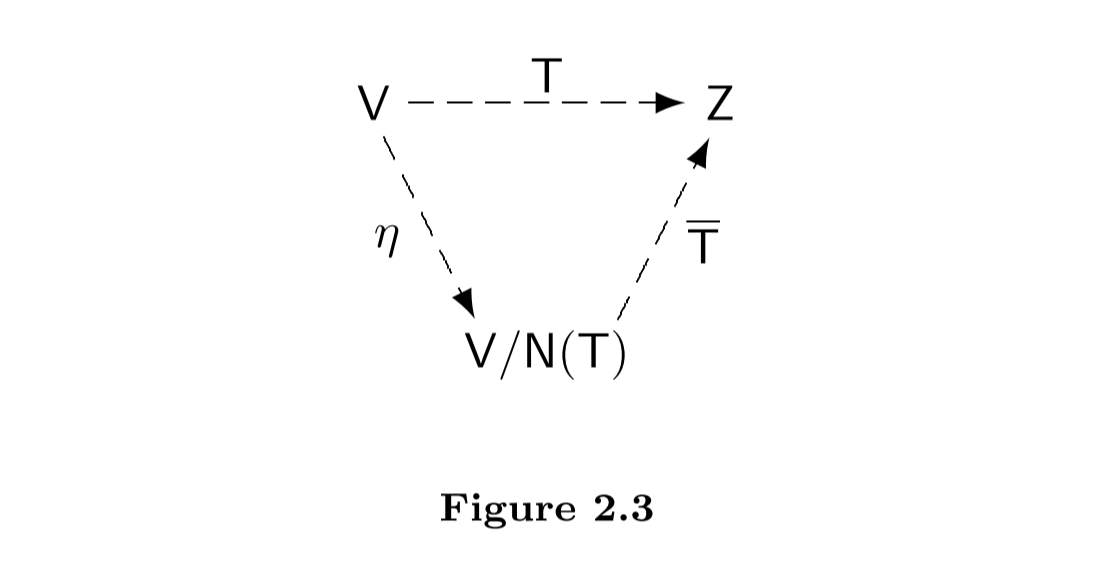
\includegraphics[width=16cm]{images/figure-2-3.png}

\begin{exercise} \label{exercise 2.4.24}
Let \(V\) and \(Z\) be vector spaces and \(\T : V \to Z\) be a linear transformation \emph{that is onto}.
Define the mapping
\[
    \overline{\T} : V / \NULLT \to Z \text{ by } \overline{\T}(v + \NULLT) = \T(v)
\]
for any coset \(v + \NULLT\) in \(V / \NULLT\).
\begin{enumerate}
\item Prove that \(\overline{\T}\) is \emph{well-defined};
    that is, prove that if \(v + \NULLT = v' + \NULLT\), then \(\T(v) = \T(v')\).
\item Prove that \(\overline{\T}\) is linear.
\item Prove that \(\overline{\T}\) is an isomorphism.
\item Prove that the diagram shown in Figure 2.3 \emph{commutes};
    that is, prove that \(\T = \overline{\T} \eta\). (\(\eta\) is defined in \EXEC{2.1.42}.)
\end{enumerate}

Note that we do not say \(V\) and \(Z\) are finite dimensional.
\end{exercise}

\begin{proof} \ 

\begin{enumerate}
\item Suppose \(v + \NULLT = v' + \NULLT\), then by \ATHM{1.10}(b), \(v - v' \in \NULLT\), which implies \(\T(v - v') = 0_{_Z}\), that is, \(\T(v) - \T(v') = 0_{_Z}\), that is, \(\T(v) = \T(v')\).

\item For any \(v_1 + \NULLT\) and \(v_2 + \NULLT\) in \(V/\NULLT\), and any scalar \(c\),
\begin{align*}
    & \overline{\T}\bigg( \big( v_1 + \NULLT \big) + c \big(v_2 + \NULLT \big)  \bigg) \\
    & = \overline{\T}\big( (v_1 + cv_2) + \NULLT) \big) & \text{by def of coset \(+\) and scalar \(\cdot\), see \EXEC{1.3.31}} \\
    & = \T(v_1 + cv_2) & \text{by def of \(\overline{\T}\)} \\
    & = \T(v_1) + c\T(v_2) & \text{since \(\T\) is linear} \\
    & = \overline{\T}(v_1 + \NULLT) + c\overline{\T}(v_2 + \NULLT), & \text{by def of \(\overline{\T}\)}
\end{align*}
hence by \ATHM{2.1}(b), \(\overline{\T}\) is linear.

\item Now we have to show \(\overline{\T}\) is one-to-one and onto.
For one-to-one, suppose \(v + \NULLT \in \NULL(\overline{\T})\), we have to show \(v + \NULLT = \OV + \NULLT\).
Then by definition of \(\overline{\T}\), \(\overline{\T}(v + \NULLT) = \T(v) = 0_{_Z}\), which implies \(v \in \NULLT\).
And of course \(v - \OV \in \NULLT\), so by \ATHM{1.10}(b), \(v + \NULLT = \OV + \NULLT\), as desired.

For onto, suppose arbitrary \(z \in Z\).
\emph{Then since \(\T\) is onto}, we can find \(v \in V\) such that \(\T(v) = z\), and for such \(v\) of course we can find \(v + \NULLT \in V/\NULLT\) such that \(\overline{\T}(v + \NULLT) = \T(v) = z\).
Hence \(\overline{\T}\) is onto.

Hence \(\overline{\T}\) is an isomorphism from \(V/\NULLT\) to \(Z\).

\item It's somewhat ambiguous that the exercise does not mention the corresponding \(W\) of the linear map \(\eta\).
Anyway, we assume \(\eta : V \to V/\NULLT\) by \(\eta(v) = v + \NULLT\).
Then for all \(v \in V\), we have
\begin{align*}
    \overline{\T}\eta(v) & = \overline{\T}(\eta(v)) & \text{by def of composition} \\
                         & = \overline{\T}(v + \NULLT) & \text{by def of \(\eta\)} \\
                         & = \T(v) & \text{by def of \(\overline{\T}\)}
\end{align*}
Hence \(\T = \overline{\T}\eta\).
\end{enumerate}
\end{proof}

\begin{exercise} \label{exercise 2.4.25}
\TODOREF{} \RED{Skip}, this need section 1.7.
\end{exercise}

\begin{proof}
\end{proof}

\begin{additional theorem} \label{athm 2.36}
This is the placeholder theorem for some matrix inversion equations:

\BLUE{(1)} \EXEC{2.4.4}: \((AB)^{-1} = B^{-1} A^{-1}\) when \(A, B\) are invertible (and compatible).

\BLUE{(2)} \EXEC{2.4.5}: \((A^\top)^{-1} = (A^{-1})^\top\) when \(A\) is invertible.
\end{additional theorem}

\begin{additional theorem} \label{athm 2.37}
This is the placeholder theorem for some judgement of zero matrix and invertibility:

\BLUE{(1)} \EXEC{2.4.6}: If \(A\) is invertible and \(AB = O\), then \(B = O\).

\EXEC{2.4.7}:

\BLUE{(2.1)}: If \(A^2 = O\) then \(A\) is not invertible.

\BLUE{(2.2)}: If \(AB = O\) for some \emph{nonzero} \(n \X n\) matrix \(B\), then \(A\) is not invertible.

\BLUE{(3)} \EXEC{2.4.9}: If \(A\) and \(B\) be \(n \X n\) matrices such that \(AB\) is invertible, then both \(A\) and \(B\) are invertible.
\end{additional theorem}

\begin{additional theorem} \label{athm 2.38}
This is the placeholder theorem for \EXEC{2.4.10}:

\BLUE{(1)}: If \(A, B\) are \(n \X n\) squares and \(AB = I_n\), then \(A, B\) are invertible, and \(A = B^{-1}\) and \(B = A^{-1}\).
In fact, we do not need to check \(BA = I_n\), hence a ``one-sided'' inverse is a ``two-sided'' inverse.

\BLUE{(2)}: Analogous result for \LTRAN{}:
Let \(\T : V \to W\) and \(\U : W \to V\) where \(V, W\) have same (finite) dimensions and \(\U\T = \ITRANV\).
Then both \(\U, \T\) are invertible. and we have \((\T)^{-1} = \U\) (hence \(\U^{-1} = \T\)).
\end{additional theorem}

\begin{additional theorem} \label{athm 2.39}
This is the placeholder theorem for \EXEC{2.4.15}:
If \(\T : V \to W\) is a \LTRAN{}, and \(\beta\) is a basis for \(V\), then \(\T\) is an isomorphism (from \(V\) to \(W\)) if and only if \(\T(\beta)\) is a basis for \(W\).
\end{additional theorem}

\begin{additional theorem} \label{athm 2.40}
This is the placeholder theorem for \EXEC{2.4.16}:
Given \(n \X n\) invertible matrix \(B\),
\(\Phi : M_{n \X n}(F) \to M_{n \X n}(F)\) by \(\Phi(A) = B^{-1}AB\) is an isomorphism.
\end{additional theorem}

\begin{additional theorem} \label{athm 2.41}
This is the placeholder theorem for \EXEC{2.4.17}:
Let \(V\) and \(W\) be finite-dimensional vector spaces and \(\T : V \to W\) be an isomorphism.
Let \(V_0\) be a \emph{subspace} of \(V\).
Then

\BLUE{(1)} \(\T(V_0)\) is a subspace of \(W\), and

\BLUE{(2)} \(\dim(V_0) = \dim(\T(V_0))\);
    we say that an isomorphism is \emph{rank-preserving}, since in particular \(\dim(V) = \dim(\T(V))\).
\end{additional theorem}

\begin{additional theorem} \label{athm 2.42}
This is the placeholder theorem for \EXEC{2.4.20}:
Let \(\T: V \to W\) be a linear transformation from an \(n\)-dimensional vector space \(V\) to an \(m\)-dimensional vector space \(W\).
Let \(\beta\) and \(\gamma\) be ordered bases for \(V\) and \(W\), respectively.
Then \(\rankT = \rank(\LMTRAN_A)\) and that \(\nullityT = \nullity(\LMTRAN_A)\), where \(A = [\T]_{\beta}^{\gamma}\).
\end{additional theorem}

\begin{additional theorem} \label{athm 2.43}
This is the placeholder theorem for \EXEC{2.4.21}, which gives an isomorphism \(\Phi_{\beta}^{\gamma} : \mathcal{L}(V, W) \to M_{m \X n}(F)\).
\end{additional theorem}

\begin{additional theorem} \label{athm 2.44}
This is the placeholder theorem for \EXEC{2.4.22}, which gives an isomorphism from \(\POLYNF\) to \(F^{n + 1}\);
And this isomorphism is related to Lagrange polynomials(or \RMK{1.6.6}).
\end{additional theorem}

\begin{additional theorem} \label{athm 2.45}
This is the placeholder theorem for \EXEC{2.4.24}, which gives some other facts about quotient space.
\end{additional theorem}
\section{The Change of Coordinate Matrix} \label{sec 2.5}

\begin{note}
Some of inverse matrices in the examples are (mysteriously) given, but in fact currently we do not know how to calculate the inverse of a invertible matrix.
This is introduced in \CH{3}.
\end{note}

In many areas of mathematics, a \emph{change of variable} is used to \emph{simplify the appearance} of an expression.
For example, in geometry the change of variable
\[
    \begin{array}{l}
        x=\frac{2}{\sqrt{5}} x^{\prime}-\frac{1}{\sqrt{5}} y^{\prime} \\
        y=\frac{1}{\sqrt{5}} x^{\prime}+\frac{2}{\sqrt{5}} y^{\prime}
\end{array}
\]
can be used to transform the equation \(2x^2 - 4xy + 5y^2 = 1\) into the simpler equation \((x')^2 + 6(y')^2 = 1\), a \emph{form} in which it is easily seen to be the equation of an ellipse. (See Figure 2.4.)

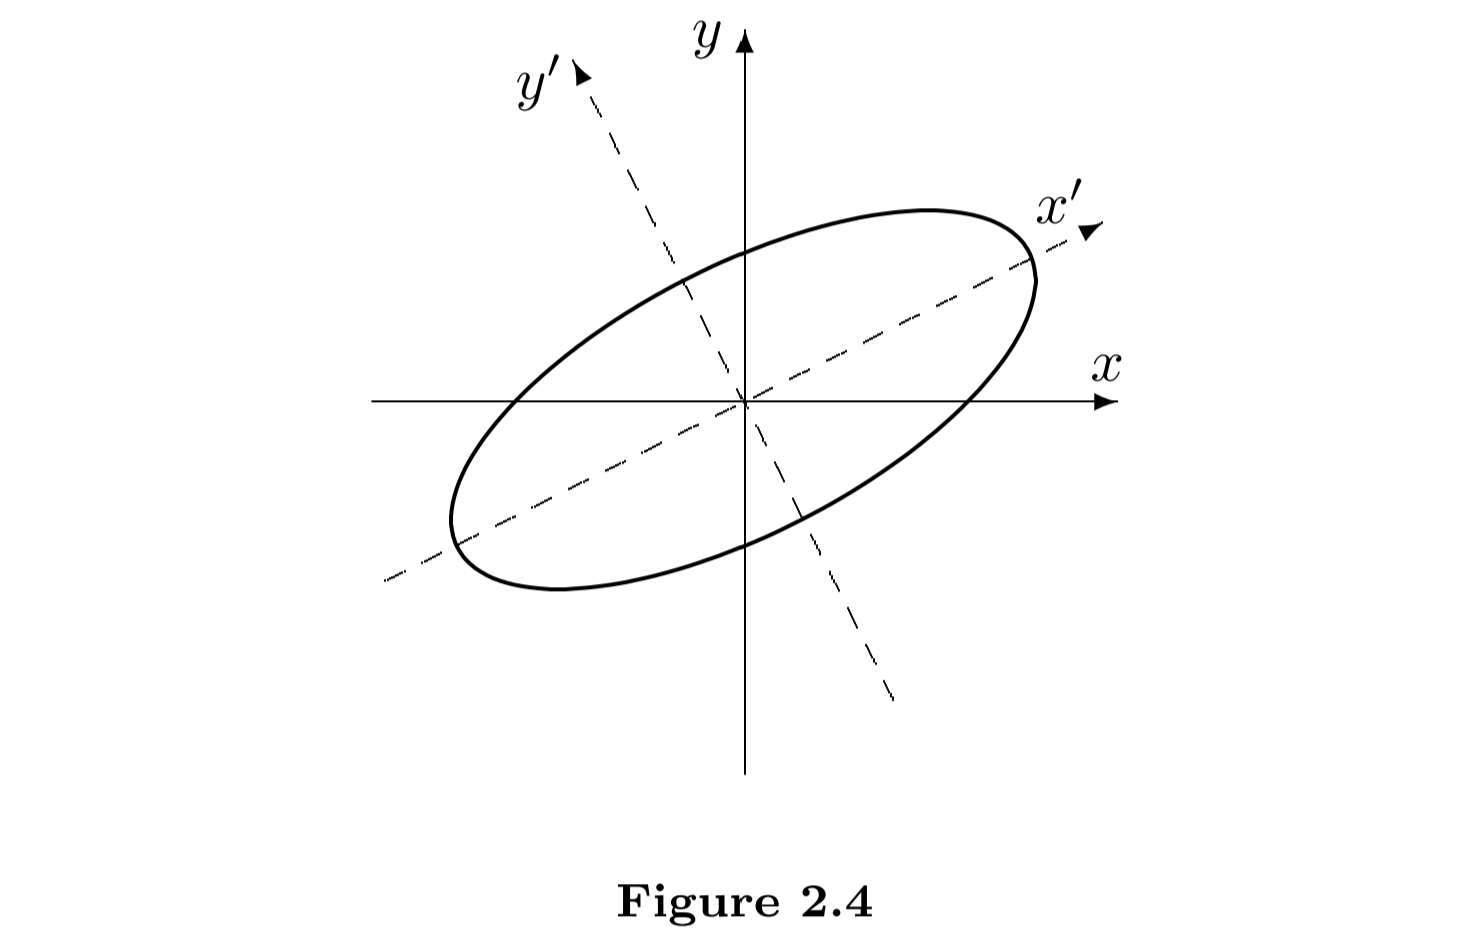
\includegraphics[width=10cm]{images/figure-2-4.png}

We will see how this change of variable is \emph{determined} in \SEC{6.5}.

(For figure 2.4,) Geometrically, the change of variable
\[
    P = \begin{pmatrix} x \\ y \end{pmatrix} \to \begin{pmatrix} x' \\ y' \end{pmatrix}
\]
is a \emph{change in the way} that the position of a point \(P\) in the plane is \emph{described}.
This is done by \emph{introducing a new frame of reference}, an \(x'y'\)-coordinate system with coordinate axes \emph{rotated} from the original \(xy\)-coordinate axes.
In this case, the new coordinate axes(\(x'\)-axis and \(y'\)-axis) are chosen to \emph{lie in the direction of the axes} of the ellipse.
The \textbf{unit vectors} along the \(x'\)-axis and the \(y'\)-axis form an \emph{ordered basis} for \(\SET{R}^2\):
\[
    \beta' = \bigg\{ \frac{1}{\sqrt{5}} \begin{pmatrix} 2 \\ 1 \end{pmatrix}, \frac{1}{\sqrt{5}} \begin{pmatrix} -1 \\ 2 \end{pmatrix} \bigg\}
\]
and the change of variable is actually a change from \([P]_{\beta} = \begin{pmatrix} x \\ y \end{pmatrix}\), the coordinate vector of \(P\) relative to the \emph{standard} ordered basis \(\beta = \{ e_1, e_2 \}\), to \([P]_{\beta'} = \begin{pmatrix} x' \\ y' \end{pmatrix}\), the coordinate vector of \(P\) relative to the new rotated basis \(\beta'\).

A natural question arises:
How can a coordinate vector relative to one basis be changed into a coordinate vector relative to the other?
Notice that the \emph{system of equations} relating the new and old coordinates can be represented by the matrix equation
\[
    \begin{pmatrix} x \\ y \end{pmatrix}
    = \frac{1}{\sqrt{5}} \begin{pmatrix}
        2 & -1 \\ 1 & 2
    \end{pmatrix} \begin{pmatrix} x' \\ y' \end{pmatrix}.
\]
Notice also that
\[
    Q = \frac{1}{\sqrt{5}} \begin{pmatrix}
        2 & -1 \\ 1 & 2
    \end{pmatrix}
\]
equals \([\mathrm{I}]_{\beta'}^{\beta}\), where \(\mathrm{I}\) denotes the \emph{identity transformation} on \(\SET{R}^2\).
Thus \([v]_{\beta} = Q[v]_{\beta'}\) for all \(v \in \SET{R}^2\).
(Also notice the \textbf{order} of the bases of the matrix representation;
the matrix representation is from the basis we want to change into the basis we originally have.)
A similar result is true in general.

\begin{theorem} \label{thm 2.22}
Let \(\beta\) and \(\beta'\) be two ordered bases for a finite-dimensional vector space \(V\), and let \(Q = [\ITRANV]_{\beta'}^{\beta}\).
Then
\begin{enumerate}
\item \(Q\) is invertible.
\item For any \(v \in V\), \([v]_{\beta} = Q[v]_{\beta'}\).
\end{enumerate}
\end{theorem}

\begin{proof} \ 

\begin{enumerate}
\item Since \(\ITRANV\) is invertible, \(Q\) is invertible by \THM{2.18}.

\item For any \(v \in V\),
\begin{align*}
    [v]_{\beta} & = [\ITRANV(v)]_{\beta} & \text{of course} \\
                & = [\ITRANV]_{\beta'}^{\beta} [v]_{\beta'} & \text{by \THM{2.14}} \\
                & = Q [v]_{\beta'}.
\end{align*}
\end{enumerate}
\end{proof}

\begin{remark} \label{remark 2.5.1}
The matrix \(Q = [\ITRANV]_{\beta'}^{\beta}\), defined in \THM{2.22}, is called \textbf{a change of coordinate matrix}.
Because of part (b) of the theorem, we say that \textbf{\(Q\) changes \(\beta'\)-coordinates into \(\beta\)-coordinates}.
Observe that if \(\beta = \{ x_1, x_2, ..., x_n \}\) and \(\beta' = \{ x'_1, x'_2, ..., x'_n \}\), then by definition of matrix representation, the \(j\)th column of \(Q = [\ITRANV]_{\beta'}^{\beta}\) is \([\ITRANV(x'_j)]_{\beta}\).
But since \([\ITRANV(x'_j)]_{\beta} = [x'_j]_{\beta}\), the \(j\)th column of \(Q\) is \([x'_j]_{\beta}\).
\end{remark}

\begin{note}
上面那段\ remark 是想表達,給定一個從原座標\ \(\beta'\) 轉換到目標座標\ \(\beta\) 的轉換矩陣,該矩陣的第\ \(j\) 行就是原座標\ \(\beta'\) 的第\ \(j\) 個\ vector,在用目標座標\ \(\beta\) 來表示時的座標向量。
\end{note}

Also notice that if \(Q\) changes \(\beta'\)-coordinates into \(\beta\)-coordinates, then \(Q^{-1}\) changes \(\beta\)-coordinates into \(\beta'\)-coordinates. (See \EXEC{2.5.11}.)

\begin{example} \label{example 2.5.1}
In \(\SET{R}^2\), let \(\beta = \{ (1, 1), (1, -1) \}\) and \(\beta' = \{ (2, 4), (3, 1) \}\).
Since
\[
    (2, 4) = 3(1, 1) - 1(1, - 1) \text{ and } (3, 1) = 2(1, 1) + 1(1, -1),
\]
The matrix that changes \(\beta\)'-coordinates into \(\beta\)-coordinates is
\[
    Q = \begin{pmatrix} 3 & 2 \\ -1 & 1 \end{pmatrix}.
\]
Thus, for instance, given a \emph{(normal) vector} \((2, 4) \in \SET{R}^2\),
\begin{align*}
    [(2, 4)]_{\beta} & = Q[(2, 4)]_{\beta'} & \text{by \THM{2.22}} \\
                     & = Q \begin{pmatrix} 1 \\ 0 \end{pmatrix} & \text{since \((2, 4)\) is the first vector of \(\beta'\)} \\
                     & = \begin{pmatrix} 3 \\ -1 \end{pmatrix} & \text{by calculation}
\end{align*}
\end{example}

\begin{note}
\((2, 4)\) in this example is \textbf{not} considered to be a coordinate vector; it simply is a ``normal'' vector of \(\SET{R}^2\).
However, \(\begin{pmatrix} 3 \\ -1 \end{pmatrix}\) is a coordinate vector;
if we consider a vector to be a coordinate vector, we write its components vertically, or horizontally but adding transpose to it.
\end{note}

For the remainder of this section, we consider only \LTRAN{}s that map a vector space \(V\) \emph{into itself}.
Such a \LTRAN{} is called a \textbf{linear operator} on \(V\).
(I have defined the term in \DEF{2.1}.)

Now suppose now that \(\T\) is a linear operator on a finite-dimensional vector space \(V\) and that \(\beta\) and \(\beta'\) are ordered bases for \(V\).
Then \(V\) can be represented by the matrices \([\T]_{\beta}\) and \([\T]_{\beta'}\).
What is the \emph{relationship} between these matrices?
The next theorem provides a simple answer using a
change of coordinate matrix.

\begin{theorem} \label{thm 2.23}
Let \(\T\) be a linear operator on a finite-dimensional vector space \(V\),
and let \(\beta\) and \(\beta'\) be ordered bases for \(V\).
Suppose that \(Q\) is the change of coordinate matrix that changes \(\beta'\)-coordinates into \(\beta\)-coordinates.
Then
\[
    [\T]_{\beta} = Q^{-1} [\T]_{\beta'} Q.
\]
\end{theorem}

\begin{note}
Related exercise: \EXEC{2.4.16}.
\end{note}

\begin{proof}
Let \(\ITRANV\) be the identity transformation on \(V\).
Then
\begin{align*}
    Q [\T]_{\beta'} & = [\ITRANV]_{\beta'}^{\beta} [\T]_{\beta'} & \text{by def of \(Q\)} \\
                    & = [\ITRANV \T]_{\beta'}^{\beta} & \text{by \THM{2.11}} \\
                    & = [\T \ITRANV]_{\beta'}^{\beta} & \text{by \THM{2.10}(c)} \\
                    & = [\T]_{\beta} [\ITRANV]_{\beta'}^{\beta} & \text{by \THM{2.11}} \\
                    & = [\T]_{\beta} Q & \text{by def of \(Q\)}
\end{align*}
which implies
\begin{align*}
             & Q [\T]_{\beta'} = [\T]_{\beta} Q \\
    \implies & Q^{-1} Q [\T]_{\beta'} = Q^{-1} [\T]_{\beta} Q & \text{by multiplying \(Q^{-1}\) on the left} \\
    \implies & [\T]_{\beta'} = Q^{-1} [\T]_{\beta} Q. & \text{of course}
\end{align*}
\end{proof}

\begin{example} \label{example 2.5.2}
Let \(\T\) be the linear operator on \(\SET{R}^2\) defined by
\[
    \T \begin{pmatrix} a \\ b \end{pmatrix} = \begin{pmatrix} 3a - b \\ a + 3b \end{pmatrix}
\]
let \(\beta = \{ (1, 1), (1, -1) \}\) and \(\beta' = \{ (2, 4), (3, 1) \}\).
The reader should verify that
\[
    [\T]_{\beta} = \begin{pmatrix} 3 & 1 \\ -1 & 3 \end{pmatrix}
\]
In \EXAMPLE{2.5.1}, we saw that the change of coordinate matrix that changes \(\beta'\)-coordinates into \(\beta\)-coordinates is
\[
    Q = \begin{pmatrix} 3 & 2 \\ -1 & 1 \end{pmatrix}.
\]
and it is easily verified that
\[
    Q^{-1} = \frac{1}{5} \begin{pmatrix} 1 & -2 \\ 1 & 3 \end{pmatrix}.
\]
Hence, by \THM{2.23},
\[
    [\T]_{\beta'} = Q^{-1} [\T]_{\beta} Q = \begin{pmatrix} 4 & 1 \\ -2 & -2 \end{pmatrix}.
\]
To show that this \([\T]_{\beta'}\) is really the correct matrix, we can verify that the image under \(\T\) of each vector of \(\beta'\) is the linear combination of the vectors of \(\beta'\) with the entries of the corresponding column as this \([\T]_{\beta'}\)'s coefficients.
For example, the image of the \emph{second} vector in \(\beta'\) is
\[
    \T \begin{pmatrix} 3 & 1 \end{pmatrix} = \begin{pmatrix} 8 & 6 \end{pmatrix} = \RED{1} \begin{pmatrix} 2 & 4 \end{pmatrix} + \RED{3} \begin{pmatrix} 3 & 1 \end{pmatrix}
\]
Notice that the coefficients of the linear combination are the entries of the \emph{second} column of this \([\T]_{\beta'}\).
\end{example}

\begin{note}
It is often useful to apply \THM{2.23} to compute \([\T]_{\beta}\), as the next example shows.
\end{note}

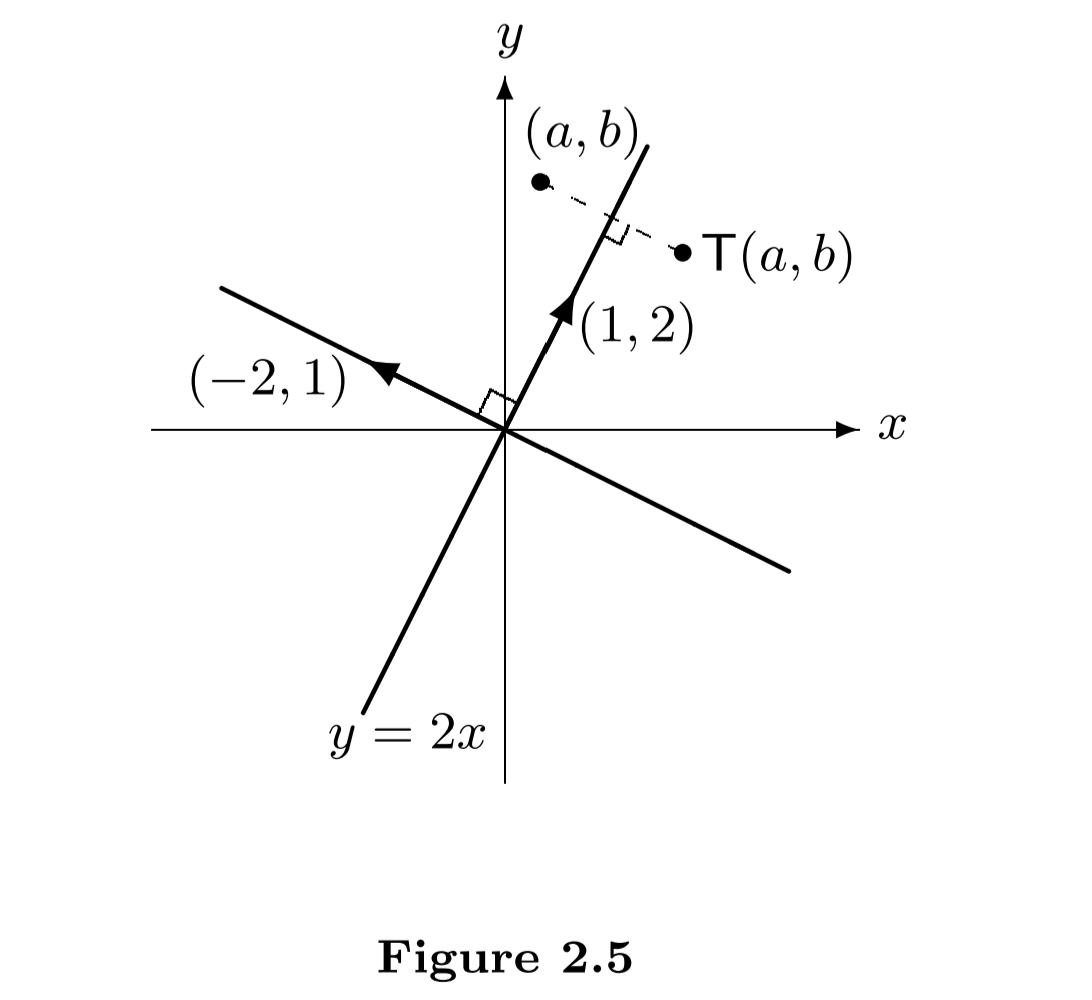
\includegraphics[width=8cm]{images/figure-2-5.png}

\begin{example} \label{example 2.5.3}
Recall the \emph{reflection} about the \(x\)-axis in \EXAMPLE{2.1.3}.
The rule \((x, y) \to (x, -y)\) is easy to obtain.
We now derive the less obvious rule for the \emph{reflection} \(\T\) \emph{about the line} \(y = 2x\). (See Figure 2.5.)

We wish to find \emph{an expression} for \(\T(a,b)\) for any \((a,b) \in \SET{R}^2\).
Since \(\T\) is linear, (by \THM{2.6}) it is completely
determined by its values on \emph{a basis} for \(\SET{R}^2\).
Clearly, from figure 2.5 we have \(\T(1, 2) = (1, 2) = 1 \cdot (1, 2) + 0 \cdot (-2, 1)\) and \(\T(-2, 1) = -(-2, 1) = 0 \cdot (1, 2) + (-1) \cdot (-2, 1)\), where \(\{ (1, 2), (-2, 1) \}\) is a basis for \(\SET{R}^2\).
Then we let \(\beta' = \{ (1, 2), (-2, 1) \}\), from these result (and \THM{2.6}),
\[
    [\T]_{\beta'} = \begin{pmatrix} 1 & 0 \\ 0 & -1 \end{pmatrix}.
\]

Now let \(\beta\) be the \emph{standard} ordered basis for \(\SET{R}^2\), and let \(Q\) be the matrix that changes \(\beta'\)-coordinates into \(\beta\)-coordinates.

Then (by calculation),
\[
    Q = \begin{pmatrix} 1 & -2 \\ 2 & 1 \end{pmatrix}
\]
And from \THM{2.23} and some calculation(see \EXEC{2.5.1}(c)) we have \([\T]_{\beta} = Q[\T]_{\beta'}Q^{-1}\).
Because (mysteriously)
\[
    Q^{-1} = \frac{1}{5} \begin{pmatrix} 1 & 2 \\ -2 & 1 \end{pmatrix}
\]
the reader can verify that
\[
    [\T]_{\beta} = \frac{1}{5} \begin{pmatrix} -3 & 4 \\ 4 & 3 \end{pmatrix}
\]
Since \(\beta\) is the standard ordered basis, it follows by \THM{2.15}(a) that \(\T\) is left-multiplication by \([\T]_{\beta}\).
Thus for any \((a, b) \in \SET{R}^2\), we have
\[
    \T \begin{pmatrix} a \\ b \end{pmatrix}
    = \frac{1}{5} \begin{pmatrix} -3 & 4 \\ 4 & 3 \end{pmatrix} \begin{pmatrix} a \\ b \end{pmatrix}
    = \frac{1}{5} \begin{pmatrix} -3a + 4b \\ 4a + 3b \end{pmatrix}.
\]
\end{example}

A useful special case of \THM{2.23} is contained in the next corollary.

\begin{corollary} \label{corollary 2.23.1}
Let \(A \in M_{n \X n}(F)\), and let \(\gamma\) be an ordered basis for \(F^n\).
Then \([\LMTRAN_A]_{\gamma} = Q^{-1} A Q\), where \(Q\) is the \(n \X n\) matrix whose \(j\)th column is the \(j\)th vector of \(\gamma\).
\end{corollary}

\begin{proof}
Let \(\beta\) be the \emph{standard} ordered basis for \(F^n\), then by \THM{2.15}(a), \([\LMTRAN_A]_{\beta} = A\).
Then by \THM{2.23}, \([\LMTRAN_A]_{\gamma} = Q^{-1} [\LMTRAN_A]_{\beta} Q\) where \(Q\) is the coordinate matrix that changes \(\gamma\)-coordinates into \(\beta\)-coordinates.
And from \RMK{2.5.1}, the \(j\)th column of \(Q\) is \([v_j]_{\beta}\) where \(v_j\) is the \(j\)th vector of \(\gamma\).
But since \(\beta\) is standard ordred basis, we have \([v_j]_{\beta} = v_j\), so the \(j\)th column of \(Q\) is \(v_j\), as desired.
\end{proof}

\begin{note}
這個\ corollary 是\ \RMK{2.5.1} 的「更加\ special case」:
當我們把某個基底座標\textbf{轉換成標準基底座標},則那個座標轉換矩陣的第\ \(j\) 行就直接等於那個基底座標的第\ \(j\) 個向量。
\end{note}

\begin{example} \label{example 2.5.4}
Let
\[
    A = \begin{pmatrix}
        2 & 1 & 0 \\ 1 & 1 & 3 \\ 0 & -1 & 0
    \end{pmatrix},
\]
and let
\[
    \gamma = \bigg\{
        \begin{pmatrix} -1 \\ 0 \\ 0 \end{pmatrix}, 
        \begin{pmatrix} 2 \\ 1 \\ 0 \end{pmatrix}, 
        \begin{pmatrix} 1 \\ 1 \\ 1 \end{pmatrix}
    \bigg\},
\]
which is an ordered basis for \(\SET{R}^3\).
Let \(Q\) be the \(3 \X 3\) matrix whose \(j\)th column is the \(j\)th vector of \(\gamma\). (this satisfies the condition of \CORO{2.23.1}.)
Then
\[
    Q = \begin{pmatrix} -1 & 2 & 1 \\ 0 & 1 & 1 \\ 0 & 0 & 1 \end{pmatrix}
    \text{ and (mysteriously) }
    Q^{-1} = \begin{pmatrix} -1 & 2 & -1 \\ 0 & 1 & -1 \\ 0 & 0 & 1 \end{pmatrix}.
\]
So by \CORO{2.23.1},
\[
    [\LMTRAN_A]_{\gamma} = Q^{-1} A Q = \begin{pmatrix} 0 & 2 & 8 \\ -1 & 4 & 6 \\ 0 & -1 & -1 \end{pmatrix}.
\]
\end{example}

\begin{remark} \label{remark 2.5.2}
The relationship, defined immediately, between the matrices \([\T]_{\beta'}\) and \([\T]_{\beta}\) in \THM{2.23} \textbf{will be the subject of further study in Chapters 5, 6, and 7}.
\end{remark}

\begin{definition} \label{def 2.16}
Let \(A\) and \(B\) be matrices in \(M_{n \X n}(F)\).
We say that \(B\) is \textbf{similar}\textbf{} to \(A\) if there exists an \textbf{invertible matrix} \(Q\) such that \(B = Q^{-1} A Q\).
\end{definition}

\begin{remark} \label{remark 2.5.3}
Observe that the relation of similarity is an \textbf{equivalence relation} (see \EXEC{2.5.9}).
So we need only say that \(A\) and \(B\) are similar.

Notice also that in this terminology \THM{2.23} can be stated as follows:
If \(\T\) is a linear operator on a finite-dimensional vector space \(V\), and if \(\beta\) and \(\beta'\) are any ordered bases for \(V\), then \([\T]_{\beta'}\) is similar to \([\T]_{\beta}\).
\end{remark}

\begin{remark} \label{remark 2.5.4}
\THM{2.23} can be \emph{generalized} to allow \(\T : V \to W\), where \(V\) is distinct from \(W\).
In this case, we can change bases in \(V\) as well as in \(W\) (see \EXEC{2.5.8}).
\end{remark}

\exercisesection

\begin{exercise} \label{exercise 2.5.1}
Label the following statements as true or false.
\begin{enumerate}
\item Suppose that \(\beta = \{ x_1, x_2, ..., x_n \}\) and \(\beta' = \{ x'_1, x'_2, ..., x'_n \}\) are ordered bases for a vector space
and \(Q\) is the change of coordinate matrix that changes \(\beta'\)-coordinates into \(\beta\)-coordinates.
Then the \(j\)th column of \(Q\) is \([x_j]_{\beta'}\).

\item Every change of coordinate matrix is invertible. 

\item Let \(\T\) be a linear operator on a finite-dimensional vector space \(V\), let \(\beta\) and \(\beta'\) be ordered bases for \(V\),
and let \(Q\) be the change of coordinate matrix that changes \(\beta'\)-coordinates into \(\beta\)-coordinates.
Then \([\T]_{\beta} = Q [\T]_{\beta'} Q^{-1}\).

\item The matrices \(A, B \in M_{n \X n}(F)\) are called similar if \(B = Q^\top A Q\) for some \(Q \in M_{n \X n}(F)\).

\item Let \(\T\) be a linear operator on a finite-dimensional vector space \(V\).
Then for any ordered bases \(\beta\) and \(\gamma\) for \(V\), \([\T]_{\beta}\) is similar to \([\T]_{\gamma}\).
\end{enumerate}
\end{exercise}

\begin{proof} \ 

\begin{enumerate}
\item False. By \RMK{2.5.1}, the \(j\)th column of \(Q\) is \([x'_j]_{\beta}\).
\item True by \THM{2.22}(a).
\item True.
    We have
    \begin{align*}
                 & [\T]_{\beta'} = Q^{-1}[\T]_{\beta}Q & \text{by \THM{2.23}} \\
        \implies & Q [\T]_{\beta'} Q^{-1} = Q (Q^{-1} [\T]_{\beta} Q) Q^{-1} & \text{by multiplying \(Q\) in the left and \(Q^{-1}\) in the right} \\
        \implies & Q [\T]_{\beta'} Q^{-1} = [\T]_{\beta},
    \end{align*}
    as desired.
\item False by \DEF{2.16}.
\item True by \RMK{2.5.3}.
\end{enumerate}
\end{proof}

\begin{exercise} \label{exercise 2.5.2}
For each of the following pairs of ordered bases \(\beta\) and \(\beta'\) for \(\SET{R}^2\), find the change of coordinate matrix that changes \(\beta'\)-coordinates into \(\beta\)-coordinates.
\begin{enumerate}
\item \(\beta = \{ e_1, e_2 \}\) and \(\beta' = \{ (a_1, a_2), (b_1, b_2) \}\).
\item \(\beta = \{ (-1, 3), (2, -1) \}\) and \(\beta' = \{ (0, 10), (5, 0) \}\).
\item \(\beta = \{ (2, 5), (-1, -3) \}\) and \(\beta' = \{ e_1, e_2 \}\).
\item \(\beta = \{ (-4, 3), (2, -1) \}\) and \(\beta' = \{ (2, 1), (-4, 1) \}\).
\end{enumerate}
\end{exercise}

\begin{proof} \ 

\begin{enumerate}
\item We have \((a_1, a_2) = a_1 \cdot e_1 + a_2 \cdot e_2\), \((b_1, b_2) = b_1 \cdot e_1 + b_2 \cdot e_2\), so
\[ Q = \begin{pmatrix} a_1 & b_1 \\ a_2 & b_2 \end{pmatrix}. \]

\item (By solving system of equations), \((0, 10) = 4 \cdot (-1, 3) + 2 \cdot (2, -1)\), \((5, 0) = 1 \cdot (-1, 3) + 3 \cdot (2, -1)\), so
\[ Q = \begin{pmatrix} 4 & 1 \\ 2 & 3 \end{pmatrix}. \]

\item (By solving system of equations), \(e_1 = 3 \cdot (2, 5) + 5 \cdot (-1, -3)\), \(e_2 = -1 \cdot (2, 5) + (-2) \cdot (-1, -3)\), so
\[ Q = \begin{pmatrix} 3 & -1 \\ 5 & -2 \end{pmatrix}. \]

\item (By solving system of equations), \((2, 1) = 2 \cdot (-4, 3) + 5 \cdot (2, -1)\), \((-4, 1) = -1 \cdot (-4, 3) + (-4) \cdot (2, -1)\), so
\[ Q = \begin{pmatrix} 2 & -1 \\ 5 & -4 \end{pmatrix}. \]
\end{enumerate}
\end{proof}

\begin{exercise} \label{exercise 2.5.3}
Skip, tedious.
\end{exercise}

\begin{exercise} \label{exercise 2.5.4}
Let \(\T\) be the linear operator on \(\SET{R}^2\) defined by
\[
    \T\begin{pmatrix} a \\ b \end{pmatrix}
    = \begin{pmatrix} 2a + b \\ a - 3b \end{pmatrix},
\]
let \(\beta\) be the standard ordered basis for \(\SET{R}^2\), and let
\[
    \beta' = \bigg\{ \begin{pmatrix} 1 \\ 1 \end{pmatrix},
    \begin{pmatrix} 1 \\ 2 \end{pmatrix} \bigg\}.
\]
Use \THM{2.23} and the (mysterious) fact that
\[
    \begin{pmatrix} 1 & 1 \\ 1 & 2 \end{pmatrix}^{-1} =
    \begin{pmatrix} 2 & -1 \\ -1 & 1 \end{pmatrix}
\]
to find \([\T]_{\beta'}\).
\end{exercise}

\begin{proof}
First \([\T]_{\beta} = \begin{pmatrix} 2 & 1 \\ 1 & -3 \end{pmatrix}\), since \(\T(e_1) = \begin{pmatrix} 2 \\ 1 \end{pmatrix}= 2 \cdot e_1 + 1 \cdot e_2\) and \(\T(e_2) = \begin{pmatrix} 1 \\ -3 \end{pmatrix} = 1 \cdot e_1 + (-3) \cdot e_2\).
And by solving equation we know \(Q = \begin{pmatrix} 1 & 1 \\ 1 & 2 \end{pmatrix}\).
Then by \THM{2.23} and the provided fact,
\[
    [\T]_{\beta'} = Q^{-1} [\T]_{\beta} Q =
    \begin{pmatrix} 2 & -1 \\ -1 & 1 \end{pmatrix}
    \begin{pmatrix} 2 & 1 \\ 1 & -3 \end{pmatrix}
    \begin{pmatrix} 1 & 1 \\ 1 & 2 \end{pmatrix}
    = \begin{pmatrix} 8 & 13 \\ -5 & -9 \end{pmatrix}
\]
\end{proof}

\begin{exercise} \label{exercise 2.5.5}
Let \(\T\) be the linear operator on \(\mathcal{P}_1(\SET{R})\) defined by \(\T(p(x)) = p'(x)\), the derivative of \(p(x)\).\
Let \(\beta = \{ 1, x \}\) and \(\beta' = \{ 1 + x, 1 - x \}\).
Use \THM{2.23} and the fact that
\[
    \begin{pmatrix} 1 & 1 \\ 1 & -1 \end{pmatrix}^{-1} =
    \begin{pmatrix} \frac1{2} & \frac1{2} \\ \frac1{2} & -\frac1{2} \end{pmatrix}
\]
to find \([\T]_{\beta'}\).
\end{exercise}

\begin{proof}

First \([\T]_{\beta} = \begin{pmatrix} 0 & 1 \\ 0 & 0 \end{pmatrix}\) since \(\T(1) = 0 = 0 \cdot 1 + 0 \cdot x\) and \(\T(x) = 1 = 1 \cdot 1 + 0 \cdot x\).
And by solving equation we know \(Q = \begin{pmatrix} 1 & 1 \\ 1 & -1 \end{pmatrix}\).
Then by \THM{2.23} and the provided fact,
\[
    [\T]_{\beta'} = Q^{-1} [\T]_{\beta} Q =
    \begin{pmatrix} \frac1{2} & \frac1{2} \\ \frac1{2} & -\frac1{2} \end{pmatrix}
    \begin{pmatrix} 0 & 1 \\ 0 & 0 \end{pmatrix}
    \begin{pmatrix} 1 & 1 \\ 1 & -1 \end{pmatrix}
    = \begin{pmatrix} \frac1{2} & -\frac1{2} \\ \frac1{2} & -\frac1{2} \end{pmatrix}
\]
\end{proof}

\begin{exercise} \label{exercise 2.5.6}
For each matrix \(A\) and ordered basis \(\beta\), find \([\LMTRAN_A]_{\beta}\).
Also, find an invertible matrix \(Q\) such that \([\LMTRAN_A]_{\beta} = Q^{-1} A Q\).

\begin{enumerate}
\item \(A = \begin{pmatrix} 1 & 3 \\ 1 & 1 \end{pmatrix}\) and \(\beta = \bigg\{
    \begin{pmatrix} 1 \\ 1 \end{pmatrix},
    \begin{pmatrix} 1 \\ 2 \end{pmatrix}
\bigg\}\)

\item \(A = \begin{pmatrix} 1 & 2 \\ 2 & 1 \end{pmatrix}\) and \(\beta = \bigg\{
    \begin{pmatrix} 1 \\ 1 \end{pmatrix},
    \begin{pmatrix} 1 \\ -1 \end{pmatrix}
\bigg\}\)

\item \(A = \begin{pmatrix} 1 & 1 & -1 \\ 2 & 0 & 1 \\ 1 & 1 & 0 \end{pmatrix}\) and \(\beta = \bigg\{
    \begin{pmatrix} 1 \\ 1 \\ 1 \end{pmatrix},
    \begin{pmatrix} 1 \\ 0 \\ 1 \end{pmatrix},
    \begin{pmatrix} 1 \\ 1 \\ 2 \end{pmatrix}
\bigg\}\)

\item \(A = \begin{pmatrix} 13 & 1 & 4 \\ 1 & 13 & 4 \\ 4 & 4 & 10 \end{pmatrix}\) and \(\beta = \bigg\{
    \begin{pmatrix} 1 \\ 1 \\ -2 \end{pmatrix},
    \begin{pmatrix} 1 \\ -1 \\ 0 \end{pmatrix},
    \begin{pmatrix} 1 \\ 1 \\ 1 \end{pmatrix}
\bigg\}\)
\end{enumerate}
\end{exercise}

\begin{proof}
From \CORO{2.23.1}, \([\LMTRAN_A]_{\beta} = Q^{-1} A Q\), where \(Q\) is the \(n \X n\) matrix whose \(j\)th column is the \(j\)th vector of \(\beta\).
Hence

\begin{enumerate}
\item \(Q = \begin{pmatrix} 1 & 1 \\ 1 & 2 \end{pmatrix}\).

\item \(Q = \begin{pmatrix} 1 & 1 \\ 1 & -1 \end{pmatrix}\).

\item \(Q = \begin{pmatrix} 1 & 1 & 1 \\ 1 & 0 & 1 \\ 1 & 1 & 2 \end{pmatrix}\).

\item \(Q = \begin{pmatrix} 1 & 1 & 1 \\ 1 & -1 & 1 \\ -2 & 0 & 1 \end{pmatrix}\).
\end{enumerate}

I skip computing \([\LMTRAN_A]_{\beta}\), since either computing it directly or using \CORO{2.23.1} but requiring \(Q^{-1}\) are tedious.
\end{proof}

\begin{exercise} \label{exercise 2.5.7}
In \(\SET{R}^2\), let \(L\) be the line \(y = mx\), where \(m \ne 0\).
Find an expression for \(\T(x, y)\), where
\begin{enumerate}
\item \(\T\) is the reflection of \(\SET{R}^2\) about \(L\).
\item \(\T\) is the projection(see \ADEF{2.2}) on \(L\) along the line \emph{perpendicular} to \(L\).
\end{enumerate}
\end{exercise}

\begin{proof}
We may let \(\beta\) be the standard ordered basis and \(\alpha = \{ (1, m), (-m, 1) \}\) be another basis for \(\SET{R}^2\).
\begin{enumerate}
\item We have that \([\T]_{\alpha} = \begin{pmatrix} 1 & 0 \\ 0 & -1 \end{pmatrix}\) and (by \EXEC{2.5.11}) \(Q^{-1} = [\mathrm{I}]_{\alpha}^{\beta} = \begin{pmatrix} 1 & m \\ -m & 1 \end{pmatrix}\).
We can also calculate that \(Q = [\mathrm{I}]_{\beta}^{\alpha} = \begin{pmatrix} \frac{1}{m^2 + 1} & \frac{m}{m^2 + 1} \\ -\frac{m}{m^2 + 1} & \frac{1}{m^2 + 1} \end{pmatrix}\).
So by \THM{2.23}, we have
\[
    [\T]_{\beta} = Q^{-1} [\T]_{\alpha} Q = \begin{pmatrix}
        \frac{1 - m^2}{m^2 + 1} & \frac{2m}{m^2 + 1} \\
        \frac{2m}{m^2 + 1} & \frac{m^2 - 1}{m^2 + 1}
    \end{pmatrix}.
\]
And we have
\begin{align*}
    & \T \begin{pmatrix} x \\ y \end{pmatrix} \\
    & = \left[ \T \begin{pmatrix} x \\ y \end{pmatrix} \right]_{\beta} & \text{since domain/codomain are actually \(\SET{R}^n\) and \(\beta\) is standard} \\
    & = [\T]_{\beta} \left[ \begin{pmatrix} x \\ y \end{pmatrix} \right]_{\beta} & \text{by \THM{2.14}} \\
    & = [\T]_{\beta} \begin{pmatrix} x \\ y \end{pmatrix} & \text{since domain/codomain are actually \(\SET{R}^n\) and \(\beta\) is standard} \\
    & = \begin{pmatrix}
            \frac{1 - m^2}{m^2 + 1} & \frac{2m}{m^2 + 1} \\
            \frac{2m}{m^2 + 1} & \frac{m^2 - 1}{m^2 + 1}
        \end{pmatrix}
        \begin{pmatrix} x \\ y \end{pmatrix} \\
    & = \begin{pmatrix}
            \frac{x-m^{2} x+2 m y}{1+m^{2}} \\
            \frac{2 m x+m^{2} y-y}{1+m^{2}}
        \end{pmatrix}
\end{align*}

\item Similarly we have that \([\T]_{\alpha} = \begin{pmatrix} 1 & 0 \\ 0 & 0 \end{pmatrix}\).
And with the same \(Q^{-1}\) and \(Q\) we have
\[
    [\T]_{\beta} = Q^{-1} [\T]_{\alpha} Q = \begin{pmatrix}
        \frac{1}{m^2 + 1} & \frac{m}{m^2 + 1} \\
        \frac{m}{m^2 + 1} & \frac{m^2}{m^2 + 1}
    \end{pmatrix}.
\]
So 
\begin{align*}
    & \T \begin{pmatrix} x \\ y \end{pmatrix} \\
    & = [\T]_{\beta} \begin{pmatrix} x \\ y \end{pmatrix} & \text{similar derivation from part(a)} \\
    & = \begin{pmatrix}
            \frac{1}{m^2 + 1} & \frac{m}{m^2 + 1} \\
            \frac{m}{m^2 + 1} & \frac{m^2}{m^2 + 1}
        \end{pmatrix}
        \begin{pmatrix} x \\ y \end{pmatrix} \\
    & = \begin{pmatrix}
            \frac{x + ym}{m^{2} + 1} \\
            \frac{xm + ym^2}{m^{2} + 1}
        \end{pmatrix}
\end{align*}

\end{enumerate}
\end{proof}

\begin{exercise} \label{exercise 2.5.8}
Prove the following \emph{generalization} of \THM{2.23}.
Let \(\T : V \to W\) be a \LTRAN{} from a finite-dimensional vector space \(V\) to a finite-dimensional vector space \(W\).
Let \(\beta\) and \(\beta'\) be ordered bases for \(V\), and let \(\gamma\) and \(\gamma'\) be ordered bases for \(W\).
Then \([\T]_{\beta'}^{\gamma'} = P^{-1} [\T]_{\beta}^{\gamma} Q\), where \(Q\) is the matrix that changes \(\beta'\)-coordinates into \(\beta\)-coordinates and \(P\) is the matrix that changes \(\gamma'\)-coordinates into \(\gamma\)-coordinates.
\end{exercise}

\begin{proof}
By (the generalization of) \THM{2.10}(c), we have \(\T = \ITRANW \T = \T \ITRANV\) \MAROON{(1)}.

Then we have
\begin{align*}
    P [\T]_{\beta'}^{\gamma'}
        & = [\ITRANW]_{\gamma'}^{\gamma} [\T]_{\beta'}^{\gamma'} & \text{by def of \(P\)} \\
        & = [\ITRANW\T]_{\beta'}^{\gamma} & \text{by \THM{2.11}} \\
        & = [\T\ITRANV]_{\beta'}^{\gamma} & \text{by \MAROON{(1)}} \\
        & = [\T]_{\beta}^{\gamma} [\ITRANV]_{\beta'}^{\beta} & \text{\THM{2.11}} \\
        & = [\T]_{\beta}^{\gamma} Q & \text{by def of \(Q\)}
\end{align*}
So we have \(P [\T]_{\beta'}^{\gamma'} = [\T]_{\beta}^{\gamma} Q\).
And
\begin{align*}
             & P [\T]_{\beta'}^{\gamma'} = [\T]_{\beta}^{\gamma} Q \\
    \implies & P^{-1} P [\T]_{\beta'}^{\gamma'} = P^{-1} [\T]_{\beta}^{\gamma} Q & \text{by multiplying \(P^{-1}\) in the left} \\
    \implies & [\T]_{\beta'}^{\gamma'} = P^{-1} [\T]_{\beta}^{\gamma} Q, & \text{of course}
\end{align*}
as desired.
\end{proof}

\begin{exercise} \label{exercise 2.5.9}
Prove that "is similar to" is an equivalence relation on \(M_{n \X n}(F)\).
\end{exercise}

\begin{proof}
For any \(n \X n\) matrix \(A\), it is similar to itself since \(A = IAI\).

Suppose \(A\) is similar to \(B\), then by \DEF{2.16} we have an invertible matrix \(Q\) s.t. \(A = Q^{-1}BQ\).
Then
\begin{align*}
             & A = Q^{-1}BQ \\
    \implies & Q A Q^{-1} = Q (Q^{-1} B Q) Q^{-1} \\
    \implies & Q A Q^{-1} = B \\
    \implies & (Q^{-1})^{-1} A Q^{-1} = B.
\end{align*}
So we have an invertible matrix \(Q^{-1}\) s.t. \(B = (Q^{-1})^{-1} A Q^{-1}\).
Then by \DEF{2.16}, \(B\) is similar to \(A\).

Suppose \(A\) is similar to \(B\), \(B\) is similar to \(C\).
Then by \DEF{2.16} we have an invertible matrix \(P\) s.t. \(A = P^{-1}BP\) and invertible matrix \(Q\) s.t. \(B = Q^{-1}CQ\)
Then by \ATHM{2.36}(2), \(QP\) is invertible and \((QP)^{-1} = P^{-1} Q^{-1}\) \MAROON{(1)}.
And
\begin{align*}
             & A = P^{-1}BP \\
    \implies & A = P^{-1} (Q^{-1} C Q) P \\
    \implies & A = (P^{-1} Q^{-1}) C (Q P) \\
    \implies & A = (Q P)^{-1} C (Q P) & \text{by \MAROON{(1)}}
\end{align*}
So we have an invertible matrix \(QP\) s.t. \(A = (QP)^{-1} C (QP)\).
So by \DEF{2.16}, \(A\) is similar to \(C\).
\end{proof}

\begin{exercise} \label{exercise 2.5.10} \ 

\begin{enumerate}
\item Prove that if \(A\) and \(B\) are similar \(n \X n\) matrices, then \(\TRACE(A) = \TRACE(B)\).
Hint: Use \ATHM{2.27}.
USEDINSEC5.2\#11.

\item How would you define the \emph{trace} of a linear operator on a finite-dimensional vector space?
Justify that your definition is well-defined.
\end{enumerate}
\end{exercise}

\begin{proof} \ 

\begin{enumerate}
\item
\begin{align*}
    \TRACE(A) & = \TRACE(\BLUE{Q^{-1}B}\RED{Q}) & \text{since \(A, B\) are similar} \\
              & = \TRACE(\RED{Q}\BLUE{Q^{-1}B}) & \text{by \ATHM{2.27}} \\
              & = \TRACE(B) & \text{of course}
\end{align*}

\item Given finite-dimensional vector space \(V\) and linear operator \(\T : V \to V\), we define \(\TRACE(\T) = \TRACE([\T]_{\beta})\) where \(\beta\) is a basis for \(V\).
The definition is well-defined because given arbitrary bases \(\beta, \beta'\) for \(V\), by \THM{2.23}, \([\T]_{\beta}\) and \([\T]_{\beta'}\) are similar, and by part(a), \(\TRACE([\T]_{\beta}) = \TRACE([\T]_{\beta'})\).
\end{enumerate}
\end{proof}

\begin{exercise} \label{exercise 2.5.11}
Let \(V\) be a finite-dimensional vector space with ordered bases \(\alpha, \beta\), and \(\gamma\).
\begin{enumerate}
\item Prove that if \(Q\) and \(R\) are the change of coordinate matrices that change \(\alpha\)-coordinates into \(\beta\)-coordinates and \(\beta\)-coordinates into \(\gamma\)-coordinates, respectively, then \(RQ\) is the change of coordinate matrix that changes \(\alpha\)-coordinates into \(\gamma\)-coordinates.

\item Prove that if \(Q\) changes \(\alpha\)-coordinates into \(\beta\)-coordinates, then \(Q^{-1}\) changes \(\beta\)-coordinates into \(\alpha\)-coordinates.
\end{enumerate}
\end{exercise}

\begin{proof} \ 
\begin{enumerate}
\item We have \(Q = [\mathrm{I}]_{\alpha}^{\beta}\) and \(R = [\mathrm{I}]_{\beta}^{\gamma}\).
So
\begin{align*}
    RQ = & [\mathrm{I}]_{\beta}^{\gamma} [\mathrm{I}]_{\alpha}^{\beta} \\
         & = [\mathrm{I}\mathrm{I}]_{\alpha}^{\gamma} & \text{by \THM{2.11}} \\
         & = [\mathrm{I}]_{\alpha}^{\gamma}, & \text{of course}
\end{align*}
which is the coordinate matrix that change \(\alpha\)-coordinates into \(\gamma\)-coordinates.

\item Again we have \(Q = [\mathrm{I}]_{\alpha}^{\beta}\).
Let \(I_n\) be \(n \X n\) identity matrix, then we have
\begin{align*}
    Q[\mathrm{I}]_{\beta}^{\alpha}
        & = [\mathrm{I}]_{\alpha}^{\beta}[\mathrm{I}]_{\beta}^{\alpha} \\
        & = [\mathrm{I}\mathrm{I}]_{\beta}^{\beta} & \text{by \THM{2.11}} \\
        & = [\mathrm{I}]_{\beta}^{\beta} & \text{of course} \\
        & = I_n, & \text{of course}
\end{align*}
and
\begin{align*}
    [\mathrm{I}]_{\beta}^{\alpha} Q
        & = [\mathrm{I}]_{\beta}^{\alpha} [\mathrm{I}]_{\alpha}^{\beta} \\
        & = [\mathrm{I}\mathrm{I}]_{\alpha}^{\alpha} & \text{by \THM{2.11}} \\
        & = [\mathrm{I}]_{\alpha}^{\alpha} & \text{of course} \\
        & = I_n, & \text{of course}
\end{align*}
hence by definition of \DEF{2.13}, \(Q^{-1}\) is \([\mathrm{I}]_{\beta}^{\alpha}\), that is, \(Q^{-1}\) is the coordinate matrix that changes \(\beta\)-coordinates into \(\alpha\)-coordinates.
\end{enumerate}
\end{proof}

\begin{exercise} \label{exercise 2.5.12}
Prove \CORO{2.23.1}.
\end{exercise}

\begin{proof}
See \CORO{2.23.1}.
\end{proof}

\begin{exercise} \label{exercise 2.5.13}
\sloppy Let \(V\) be a finite-dimensional vector space over a field \(F\), and let \(\beta = \{ x_1, x_2, ..., x_n \}\) be an ordered basis for \(V\).
Let \(Q\) be an \(n \X n\) \emph{invertible} matrix with entries from \(F\).
Define
\[
    x_j' = \sum_{i = 1}^n Q_{ij} x_i \text{ for } 1 \le j \le n,
\]
and set \(\beta' = \{ x_1', x_2', ..., x_n' \}\).
Prove that \(\beta'\) is a basis for \(V\) and hence that \(Q\) is the change of coordinate matrix that changes \(\beta'\)-coordinates into \(\beta\)-coordinates.
\end{exercise}

\begin{note}
The exercise with highly related concept: \EXEC{2.4.15}.
\end{note}

\begin{note}
這題背後的意義就是,若\ \(\beta\) 是\ basis,\(\T\) 是可逆變換(所以對應的矩陣也是可逆),則\ \(\T(\beta)\) 也是一個\ basis。
相關練習有\ \EXEC{2.4.15},不過這題是那個練習的\ special case,也就是\ codomain \(W = V\) 的情況。
\end{note}

\begin{proof}
First we show that \(\beta'\) is \LID{}.
So suppose \(a_1 x'_1 + a_2 x'_2 + ... + a_n x'_n = \OV\), we have to show \(a_1 = a_2 = ... = a_n = 0\).
Then
\begin{align*}
             & \sum_{j = 1}^n a_j x'_j = \OV \\
    \implies & \sum_{j = 1}^n a_j \bigg( \sum_{i = 1}^n Q_{ij} x_i \bigg) = \OV & \text{by def of \(x'_j\)} \\
    \implies & \sum_{j = 1}^n \bigg( \sum_{i = 1}^n Q_{ij} a_j x_i \bigg) = \OV & \text{move constant into summation} \\
    \implies & \sum_{i = 1}^n \bigg( \sum_{j = 1}^n Q_{ij} a_j x_i \bigg) = \OV, & \text{change the order of finite summation} \\
    \implies & \sum_{i = 1}^n \bigg( \sum_{j = 1}^n Q_{ij} a_j \bigg) x_i = \OV & \text{of course}
\end{align*}
which implies \(\sum_{j = 1}^n Q_{ij} a_j = 0\) for all \(1 \le i \le n\) since \(x_i\) are \LID{}.
But that implies
\begin{align*}
    \begin{pmatrix} 0 \\ 0 \\ \vdots \\ 0 \end{pmatrix}
    & = \begin{pmatrix}
        \sum_{j = 1}^n Q_{1j} a_j \\
        \sum_{j = 1}^n Q_{2j} a_j \\
        \vdots \\
        \sum_{j = 1}^n Q_{nj} a_j
    \end{pmatrix} \\
    & = Q \begin{pmatrix} a_1 \\ a_2 \\ \vdots \\ a_n \end{pmatrix} & \text{it's true but it's more intuitive from RHS to LHS}
\end{align*}
And since \(Q\) is invertible, we have
\begin{align*}
             & \begin{pmatrix} 0 \\ 0 \\ \vdots \\ 0 \end{pmatrix}
    = Q \begin{pmatrix} a_1 \\ a_2 \\ \vdots \\ a_n \end{pmatrix} \\
    \implies & \begin{pmatrix} 0 \\ 0 \\ \vdots \\ 0 \end{pmatrix} = Q^{-1} \begin{pmatrix} 0 \\ 0 \\ \vdots \\ 0 \end{pmatrix}
    = Q^{-1} Q \begin{pmatrix} a_1 \\ a_2 \\ \vdots \\ a_n \end{pmatrix} \\
    \implies & \begin{pmatrix} 0 \\ 0 \\ \vdots \\ 0 \end{pmatrix}
    = \begin{pmatrix} a_1 \\ a_2 \\ \vdots \\ a_n \end{pmatrix} \\
    \implies & a_1 = a_2 = ... = a_n = 0
\end{align*}
Hence \(\beta' = \{ x'_1, x'_2, ..., x'_n \}\) is \LID{}.
Since \(\beta'\) has \(n\) vectors, it is a basis for \(V\).

Now from the definition of \(x'_j\), we know \([x'_j]_{\beta}\) is equal to the \(j\)th column of \(Q\), but \([x'_j]_{\beta}\), which is equal to \([\mathrm{I}(x'_j)]_{\beta}\),
is (by definition of matrix representation) also equal to the \(j\)th column of \([\mathrm{I}]_{\beta'}^{\beta}\), hence \(Q = [\mathrm{I}]_{\beta'}^{\beta}\).
That is, \(Q\) is the coordinate matrix that changes \(\beta'\)-coordinates into \(\beta\)-coordinates.
\end{proof}

\begin{exercise} \label{exercise 2.5.14}
Prove the \emph{converse} of \EXEC{2.5.8}:
If \(A\) and \(B\) are each \(m \X n\) matrices with entries from a field \(F\), and if there exist \emph{invertible} \(m \X m\) and \(n \X n\) matrices \(P\) and \(Q\), respectively,
such that \(B = P^{-1} A Q\) \MAROON{(1)}, then there exist an \(n\)-dimensional vector space \(V\) and an \(m\)-dimensional vector space \(W\) (both over \(F\)), ordered bases \(\beta\) and \(\beta'\) for \(V\) and \(\gamma\) and \(\gamma'\) for \(W\),
and a \LTRAN{} \(\T : V \to W\) such that
\[
    A = [\T]_{\beta}^{\gamma} \text{ and } B = [\T]_{\beta'}^{\gamma'}.
\]
Hints: Let \(V = F^n\), \(W = F^m\), \(\T = \LMTRAN_A\), and \(\beta\) and \(\gamma\) be the \emph{standard} ordered bases for \(F^n\) and \(F^m\), respectively.
Now apply the results of \EXEC{2.5.13} to obtain ordered bases \(\beta'\) and \(\gamma'\) from \(\beta\) and \(\gamma\) via \(Q\) and \(P\), respectively.
\end{exercise}

\begin{proof}
Let \(V = F^n\), \(W = F^m\), \(\T = \LMTRAN_A\), \(\beta = \{ e_1, e_2, ..., e_n \}\) be the standard ordered basis for \(F^n\), \(\gamma = \{ f_1, f_2, ..., f_m \}\) be the standard ordered basis for \(F^m\).

Then let \(\beta' = \{ v_1, v_2, ..., v_n \}\), where \(v_j = \sum_{i = 1}^n Q_{ij} e_i\) and \(\gamma' = \{ w_1, w_2, ..., w_m \}\), where \(w_j = \sum_{i = 1}^m P_{ij} f_i\).
Then by \EXEC{2.5.13}, \(\beta', \gamma'\) are also bases for \(V\) and \(W\), respectively;
furthermore, \(Q\) is the coordinate matrix that changes \(\beta'\)-coordinates into \(\beta\) coordinates,
and \(P\) is the coordinate matrix that changes \(\gamma'\)-coordinates into \(\gamma\) coordinates.

Then since \(\beta, \gamma\) are standard bases, by \THM{2.15}(a) we have \([\T]_{\beta}^{\gamma} = [\LMTRAN_A]_{\beta}^{\gamma} = A\) \MAROON{(2)}.

And
\begin{align*}
    [\T]_{\beta'}^{\gamma'}
        & = [\LMTRAN_A]_{\beta'}^{\gamma'} \\
        & = P^{-1} [\LMTRAN_A]_{\beta}^{\gamma} Q & \text{by \EXEC{2.5.8}} \\
        & = P^{-1} A Q & \text{by \MAROON{(2)}} \\
        & = B & \text{by \MAROON{(1)}}
\end{align*}

So we have found \(V, W\), a \LTRAN{} \(\T : V \to W\), and bases \(\beta, \beta', \gamma, \gamma'\), s.t. \(A = [\T]_{\beta}^{\gamma} \text{ and } B = [\T]_{\beta'}^{\gamma'}\), as desired.
\end{proof}

\begin{additional theorem} \label{athm 2.46} \ 

\BLUE{(1)} This is the placeholder theorem for \EXEC{2.5.8}, the generalization of \THM{2.23}.

\BLUE{(2)} This is the placeholder theorem for \EXEC{2.5.14}, which is the \emph{converse} of \EXEC{2.5.8}.
\end{additional theorem}

\begin{additional theorem} \label{athm 2.47}
This is the placeholder theorem for \EXEC{2.5.9}: similarity is an equivalence relation.
\end{additional theorem}

\begin{additional theorem} \label{athm 2.48}
This is the placeholder theorem for \EXEC{2.5.10}:

\BLUE{(1)}: If \(A, B\) are similar \(n \X n\) matrices, then \(\TRACE(A) = \TRACE(B)\).

\BLUE{(2)}: Given finite-dimensional vector space \(V\) and linear operator \(\T : V \to V\), we can define \(\TRACE(\T) = \TRACE([\T]_{\beta})\) where \(\beta\) is a basis for \(V\), and the definition is well-defined.
\end{additional theorem}

\begin{additional theorem} \label{athm 2.49}
This is the placeholder theorem for \EXEC{2.5.11}:

\BLUE{(1)} If \(Q = [\mathrm{I}]_{\alpha}^{\beta}\) and \(R = [\mathrm{I}]_{\beta}^{\gamma}\), then \(RQ = [\mathrm{I}]_{\alpha}^{\gamma}\).

\BLUE{(2)} If \(Q = [\mathrm{I}]_{\alpha}^{\beta}\), then \(Q^{-1} = [\mathrm{I}]_{\beta}^{\alpha}\).
\end{additional theorem}

\begin{additional theorem} \label{athm 2.50}
This is the placeholder theorem for \EXEC{2.5.13}:

\sloppy Let \(V\) be a finite-dimensional vector space over a field \(F\), and let \(\beta = \{ x_1, x_2, ..., x_n \}\) be an ordered basis for \(V\).
Let \(Q\) be an \(n \X n\) \emph{invertible} matrix with entries from \(F\).
Define
\[
    x_j' = \sum_{i = 1}^n Q_{ij} x_i \text{ for } 1 \le j \le n,
\]
and set \(\beta' = \{ x_1', x_2', ..., x_n' \}\).
Then \(\beta'\) is a basis for \(V\) and hence that \(Q\) is the change of coordinate matrix that changes \(\beta'\)-coordinates into \(\beta\)-coordinates.
\end{additional theorem}

\chapter{Elementary Matrix Operations and Systems
of Linear Equations} \label{ch 3}

This chapter is devoted to two related objectives:
\begin{enumerate}
\item[1.] the study of certain \emph{``rank-preserving'' operations} on matrices;
\item[2.] the application of these operations and the theory of \LTRAN{}s to the \emph{solution} of systems of linear equations.
\end{enumerate}

As a consequence of objective 1, we obtain a simple method for computing the rank of a linear transformation between finite-dimensional vector spaces
\emph{by applying these rank-preserving matrix operations} to a matrix that represents that transformation.

Solving a system of linear equations is probably the most important application of linear algebra.
The familiar method of \emph{elimination} for solving systems of linear equations, which was discussed in \SEC{1.4}, involves the elimination of variables so that a simpler system can be obtained.
The technique by which the variables are eliminated \emph{utilizes three types of operations}:
\begin{enumerate}
\item [1.] interchanging any two equations in the system;
\item [2.] multiplying any equation in the system by a \emph{nonzero} constant;
\item[3.] adding a multiple of one equation to another.
\end{enumerate}

In \SEC{3.3}, we express a system of linear equations as a single matrix equation (\(Ax = b\)).
In this representation of the system, the three operations above are the ``\textbf{elementary row operations}'' for matrices(See \DEF{3.1}).
These operations provide a convenient \emph{computational} method for determining all solutions to a system of linear equations.

\section{Elementary Matrix Operations and Elementary Matrices} \label{sec 3.1}

In this section, we define the elementary operations that are used throughout the chapter.
In subsequent sections, we use these operations to obtain simple computational methods for determining the rank of a linear transformation and the solution of a system of linear equations.
There are two types of elementary matrix operations -- row operations and column operations.
As we will see, the \emph{row} operations are more useful;
they \emph{arise from} the three operations that can be \emph{used to eliminate variables} in a system of linear equations.

\begin{definition} \label{def 3.1}
Let \(A\) be an \(m \X n\) matrix.
Any one of the following three operations on the rows [columns] of \(A\) is called an \textbf{elementary row [column] operation}:
\begin{enumerate}
\item[(1)] interchanging any two rows [columns] of \(A\);
\item[(2)] multiplying any row [column] of \(A\) by a \emph{nonzero} scalar;
\item[(3)] adding any scalar multiple of a row [column] of \(A\) to \emph{other} row [column].
\end{enumerate}

Any of these three operations is called an \textbf{elementary operation}.
Elementary operations are of \textbf{type 1}, \textbf{type 2} or \textbf{type 3} depending on whether they are obtained by (1), (2), or (3).
\end{definition}

\begin{note}
I use abbreviations e.r.o. and e.c.o. to represent elementary row operation and elementary column operation, respectively.
\end{note}

\begin{example} \label{example 3.1.1}
Let
\[
    A = \begin{pmatrix}
        1 & 2 & 3 & 4 \\
        2 & 1 & -1 & 3 \\
        4 & 0 & 1 & 2
    \end{pmatrix}.
\]
Interchanging the second row of \(A\) with the first row is an example of an e.r.o. of type 1. 
The resulting matrix is
\[
    B = \begin{pmatrix}
        2 & 1 & -1 & 3 \\
        1 & 2 & 3 & 4 \\
        4 & 0 & 1 & 2
    \end{pmatrix}.
\]
Multiplying the second column of \(A\) by \(3\) is an example of an e.c.o. of type 2.
The resulting matrix is
\[
    C = \begin{pmatrix}
        1 & 6 & 3 & 4 \\
        2 & 3 & -1 & 3 \\
        4 & 0 & 1 & 2
    \end{pmatrix}.
\]
Adding \(4\) times the third row of \(A\) to the first row is an example of an e.r.o. of type 3.
In this case, the resulting matrix is
\[
    M = \begin{pmatrix}
        17 & 2 & 7 & 12 \\
        2 & 1 & -1 & 3 \\
        4 & 0 & 1 & 2
    \end{pmatrix}.
\]
\end{example}

\begin{remark} \label{remark 3.1.1}
Notice that if a matrix \(Q\) can be obtained from a matrix \(P\) by means of an e.r.o., 
then \(P\) can be obtained from \(Q\) by an e.r.o. \textbf{of the same type}.
(See \EXEC{3.1.8}.)
So, in \EXAMPLE{3.1.1}, \(A\) can be obtained from \(M\) by adding \(-4\) times the third row of \(M\) to the first row of \(M\).
\end{remark}

\begin{definition} \label{def 3.2}
An \(n \X n\) \textbf{elementary matrix} is a matrix obtained by performing an(one) elementary operation on \(I_n\).
The elementary matrix is said to be of \textbf{type 1}, \textbf{2}, or \textbf{3} according to whether the elementary operation
performed on \(I_n\) is a type 1, 2, or 3 operation, respectively.
\end{definition}

For example, interchanging the first two \emph{rows} of \(I_3\) produces the elementary matrix
\[
    E = \begin{pmatrix}
        0 & 1 & 0 \\
        1 & 0 & 0 \\
        0 & 0 & 1
    \end{pmatrix}
\]

\begin{remark} \label{remark 3.1.2}
Note that \(E\) can also be obtained by interchanging the first two \emph{columns} of \(I_3\).
In fact, any elementary matrix can be obtained in \emph{at least two ways} -- either by performing an elementary \emph{row} operation on \(I_n\) or by performing an elementary \emph{column} operation on \(I_n\).
(See \EXEC{3.1.4}.)
Similarly,
\[
    \begin{pmatrix}
        1 & 0 & -2 \\
        0 & 1 & 0 \\
        0 & 0 & 1
    \end{pmatrix}
\]
is an elementary matrix since it can be obtained from \(I_3\) by an e.c.o. of type 3
(adding \(-2\) times the first \emph{column} of \(I_3\) to the third \emph{column})
or by an e.r.o. of type 3 (adding \(-2\) times the third \emph{row} to the first \emph{row}).
\end{remark}

Our first theorem shows that \emph{performing an e.r.o. on a matrix is equivalent to multiplying the matrix by an elementary matrix}.

\begin{theorem} \label{thm 3.1}
Let \(A \in M_{m \X n}(F)\), and suppose that \(B\) is obtained from \(A\) by performing an elementary row [column] operation.
Then there exists an \(m \X m\) [\(n \X n\)] elementary matrix \(E\) such that \(B = EA\) [\(B = AE\)].
In fact, \(E\) is obtained from \(I_m\) [\(I_n\)] by \textbf{performing the same} elementary row [column] operation \textbf{as} that which was performed on \(A\) to obtain \(B\).

Conversely, if \(E\) is an elementary \(m \X m\) [\(n \X n\)] matrix, then \(EA\) [\(AE\)] is the matrix obtained from \(A\) by \textbf{performing the same} elementary row [column] operation \textbf{as} that which produces \(E\) from \(I_m\) [\(I_n\)].
\end{theorem}

\begin{proof}
See \EXEC{3.1.7}.
\end{proof}

\begin{example} \label{example 3.1.2}
Consider the matrices \(A\) and \(B\) in \EXAMPLE{3.1.1}.
In this case, \(B\) is obtained from \(A\) by interchanging the first two rows of \(A\).
Performing this \emph{same} operation on \(I_{3}\), we obtain the elementary matrix
\[
    E = \begin{pmatrix}
        0 & 1 & 0 \\
        1 & 0 & 0 \\
        0 & 0 & 1
    \end{pmatrix}
\]
Note that \(EA = B\).

In the second part of \EXAMPLE{3.1.1}, \(C\) is obtained from \(A\) by multiplying the second column of \(A\) by \(3\).
Performing this same operation on \(I_{4}\), we obtain the elementary matrix

\[
    E = \begin{pmatrix}
        1 & 0 & 0 & 0 \\
        0 & 3 & 0 & 0 \\
        0 & 0 & 1 & 0 \\
        0 & 0 & 0 & 1
    \end{pmatrix}
\]
Observe that \(AE = C\).
\end{example}

It is a useful fact that the \emph{inverse} of an elementary matrix is \emph{also} an elementary matrix.

\begin{theorem} \label{theorem} \label{thm 3.2}
Elementary matrices are \emph{invertible}, and the inverse of an elementary matrix is an elementary matrix \emph{of the same type}.
\end{theorem}

\begin{proof}
Let \(E\) be an elementary \(n \X n\) matrix.
Then (by \DEF{3.1}) \(E\) can be obtained by an e.r.o. on \(I_n\).
By \emph{reversing the steps} used to transform \(I_n\) into \(E\), we can transform \(E\) back into \(I_n\).
The result is that \(I_n\) can be obtained from \(E\) by an e.r.o. of the same type.
By \THM{3.1}, there is an elementary matrix \(\overline{E}\) such that \(\overline{E}E = I_n\).
Therefore, by \ATHM{2.38}(``one-sided'' inverse is a ``two-sided'' inverse), \(E\) is invertible and \(E^{-1} = \overline{E}\).
\end{proof}

\exercisesection

\begin{exercise} \label{exercise 3.1.1}
Label the following statements as true or false.
\begin{enumerate}
\item An elementary matrix is always square.
\item The only entries of an elementary matrix are zeros and ones. \item The \(n \X n\) identity matrix is an elementary matrix.
\item The product of two \(n \X n\) elementary matrices is an elementary matrix.
\item The inverse of an elementary matrix is an elementary matrix.
\item The sum of two \(n \X n\) elementary matrices is an elementary matrix.
\item The transpose of an elementary matrix is an elementary matrix.
\item If \(B\) is a matrix that can be obtained by performing an e.r.o. on a matrix \(A\), then \(B\) can also be obtained by performing an e.\textbf{\RED{c}}.o. on \(A\).
\item If \(B\) is a matrix that can be obtained by performing an e.r.o. on a matrix \(A\), then \(A\) can be obtained by performing an e.r.o. on \(B\).
\end{enumerate}
\end{exercise}

\begin{proof} \ 

\begin{enumerate}
\item True. Since every elementary matrix is obtained from \(I_n\) by an elementary operation that does not change the size of the matrix, and \(I_n\) is square.
\item False. \(\begin{pmatrix} 2 & 0 & 0 \\ 0 & 1 & 0 \\ 0 & 0 & 1\end{pmatrix}\) is elementary of type 2.
\item True. \(I_n\) can be considered as a type 2 elementary matrix with the first row multiplied by \(1\).
\item False. \(\begin{pmatrix} 2 & 0 \\ 0 & 1 \end{pmatrix} \begin{pmatrix} 1 & 0 \\ 0 & 2 \end{pmatrix} = \begin{pmatrix} 2 & 0 \\ 0 & 2 \end{pmatrix}\), which needs ``two'' elementary operations to obtain from \(I_2\).
\item True by \THM{3.2}.
\item False. \(\begin{pmatrix} 1 & 0 \\ 0 & 1 \end{pmatrix} + \begin{pmatrix} 1 & 0 \\ 0 & 1 \end{pmatrix} = \begin{pmatrix} 2 & 0 \\ 0 & 2 \end{pmatrix}\), which is not elementary by part(d).
\item True by \EXEC{3.1.5}.
\item False. The matrix \(\begin{pmatrix} 5 & 5 \\ 1 & 1 \end{pmatrix}\) can be obtained from \(\begin{pmatrix} 1 & 1 \\ 1 & 1 \end{pmatrix}\) by a single e.r.o. of type 3, but not by any number of \emph{column} operations, since any e.c.o. on \(\begin{pmatrix} 1 & 1 \\ 1 & 1 \end{pmatrix}\) will still leave columns that are multiple of \(\begin{pmatrix} 1 \\ 1 \end{pmatrix}\).
\item True by \EXEC{3.1.8}.
\end{enumerate}
\end{proof}

\begin{exercise} \label{exercise 3.1.2}
Let
\[
    A = \left(\begin{array}{rrr}
        1 & 2 & 3 \\
        1 & 0 & 1 \\
        1 & -1 & 1
    \end{array}\right),
    B = \left(\begin{array}{rrr}
        1 & 0 & 3 \\
        1 & -2 & 1 \\
        1 & -3 & 1
    \end{array}\right), \text { and }
    C = \left(\begin{array}{rrr}
        1 & 0 & 3 \\
        0 & -2 & -2 \\
        1 & -3 & 1
    \end{array}\right)
\]
Find an elementary operation that transforms \(A\) into \(B\) and an elementary operation that transforms \(B\) into \(C\).
\emph{By means of several additional operations}, transform \(C\) into \(I_3\).
\end{exercise}

\begin{proof}
Using type 3 e.c.o., we add column \(1\) of \(A\) times \(-2\) to column \(2\) of \(A\) to obtain \(B\);
and using type 3. e.r.o., we add row \(1\) of \(B\) times \(-1\) to row \(2\) of \(B\) to obtain \(C\);

Finally, the process of obtaining \(I_3\) from \(C\) is:
\[
    \begin{aligned}
    C & =\left(\begin{array}{ccc}
        1 & 0 & 3 \\
        0 & -2 & -2 \\
        1 & -3 & 1
    \end{array}\right)
    \rightsquigarrow
    \left(\begin{array}{ccc}
        1 & 0 & 3 \\
        0 & \RED{1} & \RED{1} \\
        1 & -3 & 1
    \end{array}\right) \\
      & \rightsquigarrow
    \left(\begin{array}{ccc}
        1 & 0 & 3 \\
        0 & 1 & 1 \\
        \RED{0} & -3 & \RED{-2}
    \end{array}\right)
    \rightsquigarrow
    \left(\begin{array}{ccc}
        1 & 0 & 3 \\
        0 & 1 & 1 \\
        0 & \RED{0} & \RED{1}
    \end{array}\right) \\
    & \rightsquigarrow
    \left(\begin{array}{ccc}
        1 & 0 & \RED{0} \\
        0 & 1 & 1 \\
        0 & 0 & 1
    \end{array}\right)
    \rightsquigarrow\left(\begin{array}{ccc}
        1 & 0 & 0 \\
        0 & 1 & \RED{0} \\
        0 & 0 & 1
    \end{array}\right)
\end{aligned}
\]
\end{proof}

\begin{exercise} \label{exercise 3.1.3}
Use the proof of \THM{3.2} to obtain the \emph{inverse} of each of the following elementary matrices.
\[
    \text{(a)} \left(\begin{array}{lll}0 & 0 & 1 \\ 0 & 1 & 0 \\ 1 & 0 & 0\end{array}\right)
    \text{ (b) } \left(\begin{array}{lll}1 & 0 & 0 \\ 0 & 3 & 0 \\ 0 & 0 & 1\end{array}\right)
    \text{ (c) } \left(\begin{array}{rrr}1 & 0 & 0 \\ 0 & 1 & 0 \\ -2 & 0 & 1\end{array}\right)
\]
\end{exercise}

\begin{proof} \ 

\begin{enumerate}
\item This is type 1 e.r.o. by changing row \(1, 3\).
So the inverse is also type 1 e.r.o. by changing row \(1, 3\) back;
that is, the inverse is \(\begin{pmatrix} 0 & 0 & 1 \\ 0 & 1 & 0 \\ 1 & 0 & 0 \end{pmatrix}\) itself.

\item This is type 2 e.r.o. by multiplying row \(2\) by \(3\).
So the inverse is type 2 e.r.o. by multiplying row \(2\) by \(\frac1{3}\);
that is, \(\begin{pmatrix} 1 & 0 & 0 \\ 0 & \frac1{3} & 0 \\ 0 & 0 & 1 \end{pmatrix}\).

\item This is type 3 e.r.o. by adding row \(1\) times \(-2\) to row \(3\).
So the inverse is type 3 e.r.o. by add row \(1\) time \(2\) to row \(3\).
that is,\(\begin{pmatrix} 1 & 0 & 0 \\ 0 & 1 & 0 \\ 2 & 0 & 1 \end{pmatrix}\).
\end{enumerate}
\end{proof}

\begin{exercise} \label{exercise 3.1.4}
Prove the assertion made on \RMK{3.1.2}:
Any elementary \(n \X n\) matrix can be obtained in at least two ways -- either by performing an e.r.o. on \(I_n\) or by performing an e.c.o. on \(I_n\).
\end{exercise}

\begin{proof}
Let \(E\) be an \(n \X n\) elementary matrix.
There are three types of elementary operations:
\begin{enumerate}
\item[1.] Interchange two columns or two rows.
\item[2.] Multiply any row or any column of \(E\) by a nonzero scalar.
\item[3.] Add any scalar multiple of a row of \(E\) to another row, or add any scalar multiple of a column of \(E\) to another column.
\end{enumerate}

We say that an elementary matrix is type (1), (2) or (3) if it is obtained performing an elementary operation type 1, 2 or 3, respectively, on \(I_n\).

If we suppose that \(E\) is type (1) and suppose that an elementary operation is performed on rows \(i\) and \(j\) of  \(I_n\),
then by interchanging \emph{columns} \(i\) and \(j\) of \(I_n\) we get the same matrix.

If we suppose that \(E\) is type (2) by multiplying row \(i\) of \(I_n\) using a nonzero scalar \(a\), than \(E\) is a matrix where all entries are same as in \(I_n\), except an item on a position \((i, i)\) in \(E\), which is equal \(a\).
If we multiply a \emph{column} \(i\) by a nonzero scalar \(a\) on \(I_n\), we can get the same matrix \(E\).

Finally, suppose that \(E\) is type (3) by multiplying row \(i\) of \(I_n\) by a nonzero scalar \(a\) and adding to row \(j\) of \(I_n\),
then \(E\) is a matrix where all entries are same as in \(I_n\), except an item on a position \((j, i)\), which is equal to \(a\).
If we multiply the \emph{column} \(j\) of \(I_n\) by the scalar \(a\) and add to the column \(i\) of \(I_n\) we can get the same matrix \(E\).

In all cases, we can find the second way to create matrix \(E\).
\end{proof}

\begin{exercise} \label{exercise 3.1.5}
Prove that \(E\) is an elementary matrix if and only if \(E^\top\) is.
\end{exercise}

\begin{proof}
We can easily check that type 1 and type 2 elementary matrices are symmetric, hence the transpose of them are also elementary matrices.

For type 3, suppose \(E\) is obtained from adding row \(i\) of \(I_n\) times scalar \(c\) to row \(j\) of \(I_n\).
Then \(E\) can be considered as \(I_n\) except that the position \((j, i)\) is equal to \(c\).
In particular, \(E^\top\) can be considered as \(I_n\) except that the position \((i, j)\) is equal to \(c\).
Then it's obvious that \(E^\top\) is obtained from adding row \(j\) of \(I_n\) times scalar \(c\) to row \(i\) of \(I_n\), so \(E^\top\) is also an elementary matrix.
\end{proof}

\begin{exercise} \label{exercise 3.1.6}
Let \(A\) be an \(m \X n\) matrix.
Prove that if \(B\) can be obtained from \(A\) by an elementary row [column] operation, then \(B^\top\) can be obtained from
\(A^\top\) by the corresponding elementary \emph{column} [row] operation.
\end{exercise}

\begin{proof}
Let
\[
    A = \begin{pmatrix} a_1 \\ a_2 \\ \vdots \\ a_m \end{pmatrix}
\]
where \(a_i\) are rows of \(A\).
Then in particular
\[
    A^\top = \begin{pmatrix} a_1^\top a_2^\top ... a_m^\top \end{pmatrix}
\]

Suppose \(B\) is obtain from \(A\) with a type 1 e.r.o., that is, changing row \(i\) and row \(j\) of \(A\) (and WLOG where \(i \le j\)).
Then \(B\) can be considered as
\[
    B = \begin{pmatrix} a_1 \\ a_2 \\ \vdots \\ \RED{a_j} \\ \vdots \\ \RED{a_i} \\ \vdots \\ a_m \end{pmatrix}
\]
Then in particular
\[
    B^\top = \begin{pmatrix} a_1^\top a_2^\top ... \RED{a_j^\top} ... \RED{a_i^\top} ... a_m^\top \end{pmatrix}
\]
which can be obtain from \(A^\top\) with a type 1 e.\RED{c}.o., that is, changing column \(i\) and column \(i\) of \(A^\top\).

Suppose \(B\) is obtain from \(A\) with a type 2 e.r.o., that is, multiplying row \(i\) of \(A\) by a nonzero scalar \(c\).
Then \(B\) can be considered as
\[
    B = \begin{pmatrix} a_1 \\ a_2 \\ \vdots \\ \RED{ca_i} \\ \vdots \\ a_m \end{pmatrix}
\]
Then in particular
\[
    B^\top = \begin{pmatrix} a_1^\top a_2^\top ... \RED{ca_i^\top} ... a_m^\top \end{pmatrix}
\]
which can be obtain from \(A^\top\) with a type 2 e.\RED{c}.o., that is, multiplying column \(i\) of \(A^\top\) by the nonzero scalar \(c\).

Finally, suppose \(B\) is obtain from \(A\) with a type 3 e.r.o., that is, adding row \(i\) of \(A\) times a scalar \(c\) to row \(j\) of \(A\).
Then \(B\) can be considered as
\[
    B = \begin{pmatrix} a_1 \\ a_2 \\ \vdots \\ \RED{ca_i + a_j} \\ \vdots \\ a_m \end{pmatrix}
\]
Then in particular
\[
    B^\top = \begin{pmatrix} a_1^\top a_2^\top ... \RED{(ca_i + a_j)^\top} ... a_m^\top \end{pmatrix} = \begin{pmatrix} a_1^\top a_2^\top ... \RED{(ca_i^\top + a_j^\top)} ... a_m^\top \end{pmatrix}
\]
(where the last equal sign is from \ATHM{1.2}(1)) which can be obtain from \(A^\top\) with a type 3 e.\RED{c}.o., that is, adding column \(i\) of \(A^\top\) times a scalar \(c\) to column \(j\) of \(A^\top\).

The case of e.c.o.s is similar to prove.
\end{proof}

\begin{exercise} \label{exercise 3.1.7}
Prove \THM{3.1}.
\end{exercise}

\begin{proof}
Let
\[
    A=\left[\begin{array}{cccc}
        a_{11} & a_{12} & \cdots & a_{1 n} \\
        a_{21} & a_{22} & \cdots & a_{2 n} \\
        \vdots & \vdots & \ddots & \vdots \\
        a_{m 1} & a_{m 2} & \cdots & a_{m n}
    \end{array}\right] \in M_{m \X n}(F)
\]

\begin{enumerate}
\item 
Suppose \(B\) is obtained from \(A\) with a type 1 e.r.o., that is, changing row \(i\) and row \(j\) of \(A\).
And if we let \(E\) be the same type of elementary matrix that changes row \(i\) and row \(j\) of \(I_n\);
that is,
\[
    E=\left[\begin{array}{cccccccc}
        1 & 0 & \cdots & 0 & \cdots & 0 & \cdots & 0 \\
        0 & 1 & \cdots & 0 & \cdots & 0 & \cdots & 0 \\
        \vdots & \vdots & \ddots & \vdots & & \vdots & & \vdots \\
        0 & 0 & \cdots & 0 & \cdots & \RED{1} & \cdots & 0 \\
        \vdots & \vdots & & \vdots & & \vdots & & \vdots \\
        0 & 0 & \cdots & \RED{1} & \cdots & 0 & \cdots & 0 \\
        \vdots & \vdots & & \vdots & & \vdots & & \vdots \\
        0 & 0 & \cdots & 0 & \cdots & 0 & \cdots & 1
    \end{array}\right] \in M_{m \X m}(F)
\]
(where the top-right \RED{\(1\)} appears in position \((i, j)\), the bottom-left \RED{\(1\)} appears in position \((j, i)\).)
Then
\[
    E A=\left[\begin{array}{cccccccc}
        a_{11} & a_{12} & \cdots & a_{1 i} & \cdots & a_{1 j} & \cdots & a_{1 n} \\
        a_{21} & a_{22} & \cdots & a_{2 i} & \cdots & a_{2 j} & \cdots & a_{2 n} \\
        \vdots & \vdots & & \vdots & & \vdots & & \vdots \\
        \RED{a_{j 1}} & \RED{a_{j 2}} & \RED{\cdots} & \RED{a_{j i}} & \RED{\cdots} & \RED{a_{j j}} & \RED{\cdots} & \RED{a_{j n}} \\
        \vdots & \vdots & & \vdots & & \vdots & & \vdots \\
        \RED{a_{i 1}} & \RED{a_{i 2}} & \RED{\cdots} & \RED{a_{i i}} & \RED{\cdots} & \RED{a_{i j}} & \RED{\cdots} & \RED{a_{i n}} \\
        \vdots & \vdots & & \vdots & & \vdots & & \vdots \\
        a_{m 1} & a_{m 2} & \cdots & a_{m i} & \cdots & a_{m j} & \cdots & a_{m n}
    \end{array}\right]
\]
is exactly the matrix obtained from changing row \(i\) and row \(j\) of \(A\); that is, \(B\).

\item
Suppose \(B\) is obtained from \(A\) with a type 2 e.r.o., that is, multiplying row \(i\) by scalar \(c\).
And if we let \(E\) be the same type of elementary matrix that multiplies row \(i\) by scalar \(c\),
that is,
\[
    E = \left[\begin{array}{ccccccc}
        1 & 0 & \cdots & 0 & 0 & \cdots & 0 \\
        0 & 1 & \cdots & 0 & 0 & \cdots & 0 \\
        \vdots & \vdots & \ddots & \vdots & \vdots & & \vdots \\
        0 & 0 & \cdots & \RED{c} & 0 & \cdots & 0 \\
        0 & 0 & \cdots & 0 & 1 & \cdots & 0 \\
        \vdots & \vdots & & \vdots & \vdots & \ddots & \vdots \\
        0 & 0 & \cdots & 0 & 0 & \cdots & 1
    \end{array}\right] \in M_{m \X m}(F)
\]
(where that red \(\RED{c}\) appears on position \((i, i)\).)
Then
\[
    E \cdot A=\left[\begin{array}{cccccc}
        a_{11} & a_{12} & \cdots & a_{1 i} & \cdots & a_{1 n} \\
        a_{21} & a_{22} & \cdots & a_{2 i} & \cdots & a_{2 n} \\
        \vdots & \vdots & & \vdots & & \vdots \\
        \RED{c a_{i 1}} &  \RED{c a_{i 2}} & \RED{\cdots} & \RED{c a_{i i}} & \RED{\cdots} & \RED{c a_{i n}} \\
        \vdots & \vdots & & \vdots & & \vdots \\
        a_{m 1} & a_{m 2} & \cdots & a_{m i} & \cdots & a_{m n}
    \end{array}\right]
\]
is exactly the matrix obtained from multiplying row \(i\) of \(A\) by scalar \(c\), that is, \(B\).

\item 
Suppose \(B\) is obtained from \(A\) with a type 3 e.r.o., that is, add row \(i\) of \(A\) times scalar \(c\) to row \(j\) of \(A\).
And if we let \(E\) be the same type of elementary matrix that adds row \(i\) of \(I_n\) times \(c\) to row \(j\) of \(I_n\);
that is,
\[
    E=\left[\begin{array}{cccccccc}
        1 & 0 & \cdots & 0 & \cdots & 0 & \cdots & 0 \\
        0 & 1 & \cdots & 0 & \cdots & 0 & \cdots & 0 \\
        \vdots & \vdots & \ddots & \vdots & & \vdots & & \vdots \\
        0 & 0 & \cdots & 1 & \cdots & 0 & \cdots & 0 \\
        \vdots & \vdots & & \vdots & & \vdots & & \vdots \\
        0 & 0 & \cdots & \RED{c} & \cdots & 1 & \cdots & 0 \\
        \vdots & \vdots & & \vdots & & \vdots & & \vdots \\
        0 & 0 & \cdots & 0 & \cdots & 0 & \cdots & 1
    \end{array}\right] \in M_{m \X m}(F)
\]
(where \RED{\(c\)} appears in position \((j, i)\).)
Then
\[
    E A= \left[\begin{array}{cccccccc}
        a_{11} & a_{12} & \cdots & a_{1 i} & \cdots & a_{1 j} & \cdots & a_{1 n} \\
        a_{21} & a_{22} & \cdots & a_{2 i} & \cdots & a_{2 j} & \cdots & a_{2 n} \\
        \vdots & \vdots & & \vdots & & \vdots & & \vdots \\
        a_{i 1} & a_{i 2} & \cdots & a_{i i} & \cdots & a_{i j} & \cdots & a_{i n} \\
        \vdots & \vdots & & \vdots & & \vdots & & \vdots \\
        \RED{a_{j 1} + c a_{i 1}} & \RED{a_{j 2} + c a_{i 2}} & \RED{\cdots} & \RED{a_{j i}+ c a_{i i}} & \RED{\cdots} & \RED{a_{j j} + c a_{i j}} & \RED{\cdots} & \RED{a_{j n}+ c a_{i n}} \\
        \vdots & \vdots & & \vdots & & \vdots & & \vdots \\
        a_{m 1} & a_{m 2} & \cdots & a_{m i} & \cdots & a_{m j} & \cdots & a_{m n}
\end{array}\right]
\]
is exactly the matrix obtained from add row \(i\) of \(A\) times scalar \(c\) to row \(j\) of \(A\), that is, \(B\).
\end{enumerate}

For elementary \emph{column} operations, if \(B \in M_{m \X n}\) is obtained from \(A \in M_{m \X n}\) by performing any type of e.c.o.,
then from \EXEC{3.1.6}, \(B^\top \in M_{n \X m}\) is obtained from \(A^\top \in M_{n \X m}\) by performing the corresponding type of e.\RED{r}.o..
Then by the previous case, we have \(B^\top = EA^\top\) \MAROON{(1)} for some elementary matrix \(E\), and
\begin{align*}
    B & = (B^\top)^\top & \text{by \ATHM{1.2}(2)} \\
      & = (EA^\top)^\top & \text{by \MAROON{(1)}} \\
      & = (A^\top)^\top E^\top & \text{by \ATHM{2.24}} \\
      & = A E^\top & \text{by \ATHM{1.2}(2)}
\end{align*}
And by \EXEC{3.1.5}, \(E^\top\) is also elementary, so we have found a elementary matrix \(E^\top\) s.t. \(B = A E^\top\), as desired.
\end{proof}

\begin{exercise} \label{exercise 3.1.8}
Prove that if a matrix \(Q\) can be obtained from a matrix \(P\) by an e.r.o., then \(P\) can be obtained from \(Q\) by an e.r.o. of the same type.
Hint: Treat each type of e.r.o. separately.
\end{exercise}

\begin{proof}
If we interchange the \(i\)th and \(j\)th rows of \(P\) to get \(Q\), we can change the \(i\)th and \(j\)th rows \(Q\) again to get \(P\), and the operation is type 1 e.r.o..

If we multiply the \(i\)th row of \(P\) by nonzero scalar \(c\) to get \(Q\), we can multiply the \(i\)th row of \(Q\) by nonzero scalar \(\frac1{c}\) to get \(P\), and the operation is type 2 e.r.o..

If we add the \(i\)th row of \(P\) times scalar \(c\), to the \(j\)th row of \(P\), to get \(Q\), then we can add the \(i\)th row of \(Q\) times scalar \(-c\), to the \(j\)th row of \(Q\), to get \(P\), and the operation is type 3 e.r.o..
\end{proof}

\begin{proof} [Another proof for \EXEC{3.1.8}]
By \THM{3.1}, we can write \(EP = Q\) where \(E\) corresponds to an e.r.o..
And by \THM{3.2}, \(E^{-1}\) is also elementary of the same type.
And
\[
    E^{-1} Q = E^{-1} E P = P.
\]
So by \THM{3.1}, \(P\) can be obtained from \(Q\) by an e.r.o. of the same type as \(E^{-1}\), which is the same type as \(E\).
\end{proof}

\begin{exercise} \label{exercise 3.1.9}
Prove that any elementary row [column] operation of type 1 can be obtained by a succession of three elementary row [column] operations of type 3 followed by one elementary row [column] operation of type 2.
\end{exercise}

\begin{proof}
Let \[A = \begin{pmatrix} a_1 \\ a_2 \\ \vdots \\ a_m \end{pmatrix}\].
Then if \(B\) can be obtain from \(A\) by performing a type 1 e.r.o., that is,
\[
    B = \begin{pmatrix} a_1 \\ a_2 \\ \vdots \\ \RED{a_j} \\ \vdots \\ \RED{a_i} \\ \vdots \\ a_m \end{pmatrix}
\]
Then
\[
    A = \begin{pmatrix} a_1 \\ a_2 \\ \vdots \\ \RED{a_i} \\ \vdots \\ \RED{a_j} \\ \vdots \\ a_m \end{pmatrix}
    \text{\RED{(*1)}} \to \begin{pmatrix} a_1 \\ a_2 \\ \vdots \\ \RED{a_i + a_j} \\ \vdots \\ \RED{a_j} \\ \vdots \\ a_m \end{pmatrix}
    \text{\RED{(*2)}} \to \begin{pmatrix} a_1 \\ a_2 \\ \vdots \\ \RED{a_i + a_j} \\ \vdots \\ \RED{-a_i} \\ \vdots \\ a_m \end{pmatrix}
    \text{\RED{(*3)}} \to \begin{pmatrix} a_1 \\ a_2 \\ \vdots \\ \RED{a_j} \\ \vdots \\ \RED{-a_i} \\ \vdots \\ a_m \end{pmatrix}
    \text{\RED{(*4)}} \to \begin{pmatrix} a_1 \\ a_2 \\ \vdots \\ \RED{a_j} \\ \vdots \\ \RED{a_i} \\ \vdots \\ a_m \end{pmatrix}
    = B
\]
where \RED{(*1)} is e.r.o. type 3 by adding row \(j\) to row \(i\);
\RED{(*2)} is e.r.o. type 3 by adding \(-1 \X\) row \(i\) to row \(j\);
\RED{(*3)} is e.r.o. type 3 by adding row \(j\) to row \(i\);
\RED{(*4)} is e.r.o. type 2 by multiplying row \(j\) by \(-1\).

The case of e.r.c. is very similar to prove.
\end{proof}

\begin{exercise} \label{exercise 3.1.10}
Prove that any elementary row [column] operation of type 2 can be obtained by dividing some row [column] by a nonzero scalar.
\end{exercise}

\begin{proof}
Well, multiplying nonzero scalar \(c\) is equal to dividing scalar \(\frac1{c}\).
\end{proof}

\begin{exercise} \label{exercise 3.1.11}
Prove that any elementary row [column] operation of type 3 can be obtained by subtracting a multiple of some row [column] from another row [column].
\end{exercise}

\begin{proof}
Well, adding a row times scalar \(c\) is equal to subtracting a row times \(c\).
\end{proof}

\begin{exercise} \label{exercise 3.1.12}
Let \(A\) be an \(m \X n\) matrix.
Prove that there exists a sequence of e.r.o.s of types 1 and 3 that transforms \(A\) into an upper triangular matrix.
\end{exercise}

\begin{proof}
The \emph{forward pass} of Gaussian elimination(see \THM{3.14}) give a sequence of e.r.o.s of type 1, 2, and 3 that transform any matrix into upper triangular.
In particular, the forward pass only uses type 2 e.r.o.s to transforms the leading term of each row into \(1\).
So if we remove type 2 e.r.o.s in the sequence, then we have found a sequence of e.r.o.s of type 1 and 3 that transforms \(A\) into an upper triangular matrix.
\end{proof}

\begin{additional theorem} \label{athm 3.1}
This is the placeholder theorem for \EXEC{3.1.5}: \(E\) is an elementary matrix if and only if \(E^\top\) is.
\end{additional theorem}

\begin{additional theorem} \label{athm 3.2}
This is the placeholder theorem for \EXEC{3.1.6}: Let \(A\) be an \(m \X n\) matrix.
If \(B\) can be obtained from \(A\) by an e.r.o. [e.c.o.], then \(B^\top\) can be obtained from \(A^\top\) by the corresponding e.c.o. [e.r.o.].
\end{additional theorem}

\begin{additional theorem} \label{athm 3.3}
This is the placeholder theorem for \EXEC{3.1.8}: If a matrix \(Q\) can be obtained from a matrix \(P\) by an e.r.o., then \(P\) can be obtained from \(Q\) by an e.r.o. of the same type.
\end{additional theorem}

\section{The Rank of a Matrix and Matrix Inverses} \label{sec 3.2}

In this section, we define the \emph{rank} of a matrix.
We then use elementary operations to compute the rank of a matrix and a \LTRAN{}.
(Recall that the definition of the rank of a \LTRAN{} is in \DEF{2.3}.)
The section concludes with \emph{a procedure for computing the inverse} of an \emph{invertible} matrix.

\begin{definition} \label{def 3.3}
If \(A \in M_{m \X n}(F)\), we define the \textbf{rank} of \(A\), denoted \(\rank(A)\), to be the rank of the \LTRAN{} \(\LMTRAN_A: F^n \to F^m\).
\end{definition}

\begin{remark} \label{remark 3.2.1}
Many results about the rank of a matrix follow immediately from the corresponding facts about a \LTRAN{}.
An important result of this type, which follows from \ATHM{2.35}(3) and \CORO{2.18.2}, (p. 103), is that \textbf{an \(n \X n\) matrix is invertible if and only if its rank is \(n\)}.
(That is, \(A\) is invertible, iff (by \CORO{2.18.2}) \(\LMTRAN_A\) is invertible, iff (by \ATHM{2.35}(3)) \(\rank(\LMTRAN_A) = \dim(F^n) = n\).) 
\end{remark}

\begin{remark} \label{remark 3.2.2}
Every matrix \(A\) is the matrix representation of the \LTRAN{} \(\LMTRAN_A\) with respect to the appropriate \emph{standard} ordered bases.
(See \THM{2.15}(a).)
And by \DEF{3.3} we have \(\rank(A) = \rank(\LMTRAN_A)\).
Thus the rank of the linear transformation \(\LMTRAN_A\) is the same as the rank of \RED{\textbf{one of}} its matrix representations, namely, \(A\).
The next theorem extends this fact to \RED{\textbf{any}} matrix representation of any linear transformation defined on finite-dimensional vector spaces.
\end{remark}

\begin{theorem} \label{thm 3.3}
Let \(\T : \V \to \W\) be a \LTRAN{} between finite-dimensional vector spaces, and let \(\beta\) and \(\gamma\) be \emph{arbitrary} ordered bases for \(\V\) and \(\W\), respectively.
Then \(\rankT = \rank([\T]_{\beta}^{\gamma})\).
\end{theorem}

\begin{proof}
From \ATHM{2.42}, we have \(\rankT = \rank(\LMTRAN_A)\) where \(A = [\T]_{\beta}^{\gamma}\).
But by \DEF{3.3}, \(\rank(A) = \rank(\LMTRAN_A)\), so we have \(\rankT = \rank(A)\);
that is, \(\rankT = \rank([\T]_{\beta}^{\gamma})\).
\end{proof}

\begin{proof}[Another proof for \THM{3.3}]
This proof uses \ATHM{2.41}(2), which is the hint of \ATHM{2.42}.
(I think it's more intuitive to use \ATHM{2.41}(2) in this context.)

Again let \(A = [\T]_{\beta}^{\gamma}\).
So, from \RMK{2.4.6}, we have \(\phi_{\gamma} \T = \LMTRAN_A \phi_{\beta}\), which (of course) implies \(\T = \phi_{\gamma}^{-1} \LMTRAN_A \phi_{\beta}\) \MAROON{(1)}.
Then
\begin{align*}
    \rankT & = \dim(\RANGET) = \dim(\T(\V)) & \text{just by definition} \\
           & = \dim(\phi_{\gamma}^{-1} \LMTRAN_A \phi_{\beta}(\V)) & \text{by \MAROON{(1)}} \\
           & = \dim(\phi_{\gamma}^{-1} \LMTRAN_A (\phi_{\beta}(\V))) & \text{by def of composition} \\
           & = \dim(\phi_{\gamma}^{-1} \LMTRAN_A (F^n)) & \text{since in particular \(\phi_{\beta}\) is onto} \\
           & = \dim(\phi_{\gamma}^{-1} (\LMTRAN_A (F^n))) & \text{by def of composition} \\
           & = \dim(\LMTRAN_A (F^n)) & \text{by \ATHM{2.41}(2),} \\
           & & \text{and since \(\phi_{\gamma}^{-1}\) is also an isomorphism} \\
           & = \dim(\RANGE(\LMTRAN_A)) = \rank(\LMTRAN_A) & \text{just by definition} \\
           & = \rank(A) & \text{by \DEF{3.3}} \\
           & = \rank([\T]_{\beta}^{\gamma})
\end{align*}
\end{proof}

\begin{remark} \label{remark 3.2.3}
Now that from \THM{3.3}, the problem of finding the rank of a \LTRAN{} has been \emph{reduced to} the problem of finding the rank of a matrix.
But given a matrix representation \(A\) of a \LTRAN{}, it could be difficult to compute its rank;
(that is, it could also be difficult to compute \(\rank(\LMTRAN_A)\))
but we can perform some \emph{``rank-preserving''} operations on the matrix to get a matrix of which it is easy to compute the rank.
The next theorem and its corollary tell us how to do this.
\end{remark}

\begin{theorem} \label{thm 3.4}
Let \(A\) be an \(m \X n\) matrix.
If \(P\) and \(Q\) are \textbf{invertible} \(m \X m\) and \(n \X n\) matrices, respectively,
then
\begin{enumerate}
\item \(\rank(AQ) = \rank(A)\),
\item \(\rank(PA) = \rank(A)\), and \emph{therefore},
\item \(\rank(PAQ) = \rank(A)\).
\end{enumerate}
\end{theorem}

\begin{proof}
First observe that
\begin{align*}
    \rank(AQ) & = \rank(\LMTRAN_{AQ}) & \text{by \DEF{3.3}} \\
              & = \dim(\RANGE(\LMTRAN_{AQ})) & \text{by def of rank of \LTRAN{}} \\
              & = \dim(\RANGE(\LMTRAN_A \LMTRAN_Q)) & \text{by \THM{2.15}(e)} \\
              & = \dim(\LMTRAN_A \LMTRAN_Q(F^n)) & \text{by def of range} \\
              & = \dim(\LMTRAN_A(\LMTRAN_Q(F^n))) & \text{by def of composition} \\
              & = \dim(\LMTRAN_A(F^n)) & \text{\(Q\) invertible, so \(\LMTRAN_Q\) invertible, and in particular onto} \\
              & = \dim(\RANGE(\LMTRAN_A)) & \text{by def of range} \\
              & = \rank(\LMTRAN_A) & \text{by def of rank of \LTRAN{}} \\
              & = \rank(A) & \text{by \DEF{3.3}}
\end{align*}
This establishes part(a).

To establish part(b),
\begin{align*}
    \rank(PA) & = \rank(\LMTRAN_{PA}) & \text{by \DEF{3.3}} \\
              & = \rank(\LMTRAN_P \LMTRAN_A) & \text{by \THM{2.15}(e)} \\
              & = \dim(\RANGE(\LMTRAN_P \LMTRAN_A)) & \text{by def of rank of \LTRAN{}} \\
              & = \dim(\LMTRAN_P \LMTRAN_A(F^n)) & \text{by def of range} \\
              & = \dim(\LMTRAN_P(\LMTRAN_A(F^n)) & \text{by def of composition} \\
              & = \dim(\LMTRAN_A(F^n)) & \text{by \ATHM{2.41}(2),} \\
              & & \text{since (\(P\) is invertible then) \(\LMTRAN_P\) is invertible} \\
              & = \dim(\RANGE(\LMTRAN_A)) & \text{by def of range} \\
              & = \rank(\LMTRAN_A) & \text{by def of rank of \LTRAN{}} \\
              & = \rank(A) & \text{by \DEF{3.3}}
\end{align*}

Finally, applying (a) and (b), we have
\begin{align*}
    \rank(PAQ) & = \rank((PA)Q) & \text{of course} \\
               & = \rank(PA) & \text{by part(a)} \\
               & = \rank(A). & \text{by part(b)}
\end{align*}
\end{proof}

\begin{corollary} \label{corollary 3.4.1}
Elementary row and column operations on a matrix are \emph{rank-preserving}.
\end{corollary}

\begin{proof}
If \(B\) is obtained from a matrix \(A\) by an elementary row operation, then by \THM{3.1} there exists an elementary matrix \(E\) such that \(B = EA\).
By \THM{3.2}, \(E\) is invertible, and hence \(\rank(B) = \rank(EA) = \rank(A)\) by \THM{3.4}(b).

If \(B\) is obtained from a matrix \(A\) by an elementary column operation, then again by \THM{3.1} there exists an elementary matrix \(E\) such that \(B = AE\).
By \THM{3.2}, \(E\) is invertible, and hence \(\rank(B) = \rank(AE) = \rank(A)\) by \THM{3.4}(a).
\end{proof}

Now that we have a class of matrix operations(i.e., e.r.o. and e.c.o.) that preserve rank, we need a way of \emph{examining a transformed matrix to ascertain its rank}.
The next theorem is the first of several in this direction.

\begin{note}
這邊的脈絡是,直接把一個\ \LTRAN{} 寫成矩陣代表,我們常常還是不容易看出該矩陣的\ rank。
但我們現在要給定一些方法使得我們可以很輕易的判斷某些類型的矩陣的\ rank。
然後再用\ e.r.o. (跟\ e.c.o.) 這些\ rank-preserving 操作把那個矩陣代表轉成這類型的矩陣,判斷這類矩陣的\ rank,就能得到原本的矩陣代表的\ rank 了。
\end{note}

\begin{theorem} \label{thm 3.5}
The rank of any matrix equals the \emph{maximum} number of its \emph{\LID{}} columns;
that is, the rank of a matrix is the \emph{dimension of the subspace generated by its columns}.
\end{theorem}

\begin{note}
In the theorem above, the second statement is equivalent to the first statement, but it needs proof;
however, it's trivial(proof by contradiction).
And the proof below just proves the second statement.
\end{note}

\begin{note}
有了這個定理,我們就不用去看\ \(\LMTRAN_A\) 的\ rank 來得出\ \(A\) 的\ rank,而是可直接從「\(A\) 的長相」或者\ \(A\) 的\ columns span 出來的\ subspace(的\ dimension) 來知道\ \(A\) 的\ rank。
\end{note}

\begin{proof}
Let arbitrary \(A \in M_{m \X n}(F)\),
\(a_1, a_2, ..., a_n\) be the columns of \(A\),
and \(\beta = \{ e_1, e_2, ..., e_n \}\) be the \emph{standard} ordered basis for \(F^n\).
Then
\begin{align*}
    \rank(A) & = \rank(\LMTRAN_A) & \text{by \DEF{3.3}} \\
             & = \dim(\RANGE(\LMTRAN_A)) & \text{by def of rank of \LTRAN{}} \\
             & = \dim(\spann(\LMTRAN_A(\beta))) & \text{by \THM{2.2}} \\
             & = \dim(\spann(\{ \LMTRAN_A(e_1), \LMTRAN_A(e_2), ..., \LMTRAN_A(e_n) \})) \\
             & = \dim(\spann(\{ Ae_1, Ae_2, ..., Ae_n \})) & \text{just by def of left multiplication} \\
             & = \dim(\spann(\{ a_1, a_2, ..., a_n \})) & \text{by \THM{2.13}(b)}
\end{align*}
\end{proof}

\begin{example} \label{example 3.2.1}
Let
\[
    A=\left(\begin{array}{lll}
        1 & 0 & 1 \\
        0 & 1 & 1 \\
        1 & 0 & 1
    \end{array}\right)
\]
Observe that the first and second columns of \(A\) are \LID{} and that the third column is a linear combination of the first two.

Thus
\[
    \rank(A) =
    \dim
        \left(
        \spann\left(\left\{
            \left(\begin{array}{l}
                1 \\
                0 \\
                1
            \end{array}\right),
            \left(\begin{array}{l}
                0 \\
                1 \\
                0
            \end{array}\right),
            \left(\begin{array}{l}
                1 \\
                1 \\
                1
            \end{array}
        \right)\right\}\right)
        \right)
    = 2
\]
\end{example}

\begin{remark} \label{remark 3.2.4}
To compute the rank of a matrix \(A\), it is frequently useful to \emph{postpone the use of \THM{3.5}} until \(A\) has been suitably \emph{modified by} means of appropriate \emph{elementary row and column operations} so that the number of \LID{} columns is obvious.
\CORO{3.4.1} guarantees that the rank of the modified matrix is the same as the rank of \(A\).

One such modification of \(A\) can be obtained by using elementary row and column operations to \emph{introduce zero entries}.
The next example illustrates this procedure.
\end{remark}

\begin{example} \label{example 3.2.2}
Let
\[
    A = \begin{pmatrix} 1 & 2 & 1 \\ 1 & 0 & 3 \\ 1 & 1 & 2 \end{pmatrix}.
\]
If we subtract the first row of \(A\) from rows 2 and 3 (type 3 elementary row operations), the result is
\[
    \begin{pmatrix} 1 & 2 & 1 \\ \RED{0} & -2 & 2 \\ \RED{0} & -1 & 1 \end{pmatrix}.
\]
If we now subtract twice the first \emph{column} from the second and subtract the first \emph{column} from the third (type 3 elementary \emph{column} operations), we obtain
\[
    \begin{pmatrix} 1 & \RED{0} & \RED{0} \\ 0 & -2 & 2 \\ 0 & -1 & 1 \end{pmatrix}.
\]
It is now obvious that the maximum number of \LID{} columns of this matrix is \(2\).
Hence the rank of \(A\) is \(2\).
\end{example}

The next theorem uses this process to transform a matrix into a particularly simple form.
The power of this theorem can be seen in its corollaries.

\begin{theorem} \label{thm 3.6}
Let \(A\) be an \(m \X n\) matrix and its rank is \(r\).

\BLUE{(1)} Then by means of a \emph{finite} number of elementary row and column operations, \(A\) can be transformed into the matrix
\[
    D = \begin{pmatrix} I_r & O_1 \\ O_2 & O_3 \end{pmatrix}
\]
where \(O_1, O_2\), and \(O_3\) are zero matrices.
Furthermore, \(r \le m\) \textbf{and} \(r \le n\), which is a direct consequence of \BLUE{(1)} since trivially by \THM{3.5}, \(\rank(D) = r\), and by \CORO{3.4.1}, \(\rank(A) = \rank(D)\), and from the structure of \(D\) we have \(r \le m\) and \(r \le n\).
Thus \(D_{ii} = 1\) for \(i \le r\) and \(D_{ij} = 0\) otherwise.
\end{theorem}

\THM{3.6} and its corollaries are quite important.
Its proof, though easy to understand, is tedious to read.
As an aid in following the proof, we first consider an example.

\begin{example} \label{example 3.2.3}
Consider the matrix
\[
    A = \begin{pmatrix} 0 & 2 & 4 & 2 & 2 \\ 4 & 4 & 4 & 8 & 0 \\ 8 & 2 & 0 & 10 & 2 \\ 6 & 3 & 2 & 9 & 1 \end{pmatrix}.
\]
By means of a succession of elementary row and column operations, we can transform \(A\) into a matrix \(D\) as in \THM{3.6}.
We list many of the intermediate matrices, but on several occasions a matrix is transformed from the preceding one by means of \emph{several} elementary operations.
The number above each arrow indicates how many elementary operations are involved. Try to identify the nature of each elementary operation (row or column and type) in the following matrix transformations
\begin{align*}
    \left(\begin{array}{rrrrr}
        0 & 2 & 4 & 2 & 2 \\
        4 & 4 & 4 & 8 & 0 \\
        8 & 2 & 0 & 10 & 2 \\
        6 & 3 & 2 & 9 & 1
    \end{array}\right) \stackrel{1\MAROON{(1)}}{\longrightarrow}
    \left(\begin{array}{rrrrr}
        4 & 4 & 4 & 8 & 0 \\
        0 & 2 & 4 & 2 & 2 \\
        8 & 2 & 0 & 10 & 2 \\
        6 & 3 & 2 & 9 & 1
    \end{array}\right) \stackrel{1\MAROON{(2)}}{\longrightarrow}
    \left(\begin{array}{rrrrr}
        1 & 1 & 1 & 2 & 0 \\
        0 & 2 & 4 & 2 & 2 \\
        8 & 2 & 0 & 10 & 2 \\
        6 & 3 & 2 & 9 & 1
    \end{array}\right) \stackrel{2\MAROON{(3)}}{\longrightarrow} \\
    \left(\begin{array}{rrrrrr}
        1 & 1 & 1 & 2 & 0 \\
        0 & 2 & 4 & 2 & 2 \\
        0 & -6 & -8 & -6 & 2 \\
        0 & -3 & -4 & -3 & 1
    \end{array}\right) \stackrel{3\MAROON{(4)}}{\longrightarrow}
    \left(\begin{array}{rrrrrr}
        1 & 0 & 0 & 0 & 0 \\
        0 & 2 & 4 & 2 & 2 \\
        0 & -6 & -8 & -6 & 2 \\
        0 & -3 & -4 & -3 & 1
    \end{array}\right) \stackrel{1\MAROON{(5)}}{\longrightarrow} \\
    \left(\begin{array}{rrrrrr}
        1 & 0 & 0 & 0 & 0 \\
        0 & 1 & 2 & 1 & 1 \\
        0 & -6 & -8 & -6 & 2 \\
        0 & -3 & -4 & -3 & 1
    \end{array}\right) \stackrel{2\MAROON{(6)}}{\longrightarrow}
    \left(\begin{array}{rrrrr}
        1 & 0 & 0 & 0 & 0 \\
        0 & 1 & 2 & 1 & 1 \\
        0 & 0 & 4 & 0 & 8 \\
        0 & 0 & 2 & 0 & 4
    \end{array}\right) \stackrel{3\MAROON{(7)}}{\longrightarrow}
    \left(\begin{array}{rrrrrr}
        1 & 0 & 0 & 0 & 0 \\
        0 & 1 & 0 & 0 & 0 \\
        0 & 0 & 4 & 0 & 8 \\
        0 & 0 & 2 & 0 & 4
    \end{array}\right) \stackrel{1\MAROON{(8)}}{\longrightarrow} \\
    \left(\begin{array}{rrrrr}
        1 & 0 & 0 & 0 & 0 \\
        0 & 1 & 0 & 0 & 0 \\
        0 & 0 & 1 & 0 & 2 \\
        0 & 0 & 2 & 0 & 4
    \end{array}\right) \stackrel{1\MAROON{(9)}}{\longrightarrow}
    \left(\begin{array}{rrrrr}
        1 & 0 & 0 & 0 & 0 \\
        0 & 1 & 0 & 0 & 0 \\
        0 & 0 & 1 & 0 & 2 \\
        0 & 0 & 0 & 0 & 0
    \end{array}\right) \stackrel{1\MAROON{(10)}}{\longrightarrow}
    \left(\begin{array}{rrrrr}
        1 & 0 & 0 & 0 & 0 \\
        0 & 1 & 0 & 0 & 0 \\
        0 & 0 & 1 & 0 & 0 \\
        0 & 0 & 0 & 0 & 0
    \end{array}\right) = D
\end{align*}
\begin{enumerate}
\item[\MAROON{(1)}] one e.r.o.(1), changing row 1 and row 2.
\item[\MAROON{(2)}] one e.r.o.(2), multiplying \(1/4\) to row 1
\item[\MAROON{(3)}] two e.r.o.(3), subtracting row 3, 4 from row 1
\item[\MAROON{(4)}] three e.c.o.(3), subtracting col 1 from col 2, 3, 4
\item[\MAROON{(5)}] one e.r.o.(2), multiplying \(1/2\) to row 2
\item[\MAROON{(6)}] two e.r.o.(3), subtracting row 2 from row 3, 4
\item[\MAROON{(7)}] three e.c.o.(3), subtracting row 2 from col 3, 4, 5
\item[\MAROON{(8)}] one e.r.o.(2), multiplying \(1/4\) to row 3
\item[\MAROON{(9)}] one e.r.o.(3), subtracting row 3 from row 4
\item[\MAROON{(10)}] one e.c.o.(3), subtracting col 3 from col 5
\end{enumerate}
By the \CORO{3.4.1}, \(\rank(A) = \rank(D)\).
Clearly, however, \(\rank(D) = 3\); so \(\rank(A) = 3\).
\end{example}

\begin{note}
Note that the first two elementary operations in \EXAMPLE{3.2.3} result in a \(1\) in the \(1,1\) position,
and the next several operations (type 3) result in \(O\)'s everywhere in the first row and first column except for the \(1,1\) position.
\emph{And the remaining elementary operations do not change the first row and first column}.
With this example in mind, we proceed with the proof of \THM{3.6}.
\end{note}

\begin{proof}[Proof for \THM{3.6}]
If \(A\) is the zero matrix, \(r = 0\) by \EXEC{3.2.3} and of course \(r \le m\) and \(r \le n\).
In this case, the conclusion follows with \(D = A\).

Now suppose that \(A \ne O_{m \X n}\) and \(r = \rank(A)\);
then \(r > 0\).
The proof is by mathematical induction on \(m\), the number of rows of \(A\).

Suppose that \(m = 1\).
We construct a sequence of finite operations to transform \(A\) into a matrix of the desired form.
By means of at most one type 1 column operation and at most one type 2 column operation, \(A\) can be transformed into a matrix with a \(1\) in the 1,1 position.
By means of at most \(n - 1\) type 3 column operations, this matrix can in turn be transformed into the matrix
\[
    \begin{pmatrix} 1 & 0 & ... & 0 \end{pmatrix},
\]
which has the desired form.
And note that there is one \LID{} \emph{column} in \(D\).
So
\begin{align*}
    \rank(A) & = \rank(D) & \text{by the \CORO{3.4.1}} \\
             & = 1. & \text{by \THM{3.5}}
\end{align*}
Hence \(\rank(A) \le 1\), the number of rows of \(A\), and \(\rank(A) \le n\), the number of columns of \(A\).
Thus the theorem is established for \(m = 1\).

Next assume that the theorem holds for any matrix with \(m - 1\) rows (for some \(m > 1\)).
We must prove that the theorem holds for any matrix with \(m\) rows.

Suppose that \(A\) is any \(m \X n\) matrix.
If \(n = 1\), \THM{3.6} can be established in a manner analogous to that for \(m = 1\) (see \EXEC{3.2.10}).

We now suppose that \(n > 1\).
Since \(A \ne O_{m \X n}\), \(A_{ij} \ne 0\) for \emph{some} \(i, j\).
By means of at most one e.r.o. and at most one e.c.o. (each of type 1), we can move the nonzero entry to the \(1,1\) position (just as was done in \EXAMPLE{3.2.3}).
By means of at most one additional type 2 operation, we can assure a \(1\) in the \(1,1\) position.
(Look at the second operation in \EXAMPLE{3.2.3}.)
By means of at most \(m - 1\) type 3 row operations and at most \(n - 1\) type 3 column operations,
we can eliminate all nonzero entries in the first row and the first column with the exception of the \(1\) in the \(1,1\) position.
(In \EXAMPLE{3.2.3}, we used two row and three column operations to do this.)
Thus, with a finite number of elementary operations, \(A\) can be transformed into a matrix
\[
    B= \left(\begin{array}{c|ccc}
        1 & 0 & \cdots & 0 \\
        \hline 0 & & & \\
        \vdots & & B^{\prime} & \\
        0 & & &
    \end{array}\right)
\]
where \(B'\) is an \(\RED{(m - 1)} \X (n - 1)\) matrix.
In \EXAMPLE{3.2.3}, for instance,
\[
    B' = \begin{pmatrix}
        2 & 4 & 2 & 2 \\
        -6 & -8 & -6 & 2 \\
        -3 & -4 & -3 & 1
    \end{pmatrix}.
\]
By \EXEC{3.2.11}, \(B'\) must have rank \emph{one less than} \(B\).
Since \(\rank(A) = \rank(B) = r\), \(\rank(B') = r - 1\).
Also by the \emph{induction hypothesis}, \(B'\) can be transformed by a \emph{finite} number of elementary row and column operations into the \((m - 1) \X (n - 1)\) matrix \(D'\) such that
\[
    D' = \begin{pmatrix}
        I_{r - 1} & O_4 \\
        O_5 & O_6
    \end{pmatrix}
\]
where \(O_4, O_5,\) and \(O_6\) are zero matrices, and \(r - 1 \le m - 1\) and \(r - 1 \le n - 1\).
And the latter simply implies \(r \le m\) and \(r \le n\).
That is, \(D'\) consists of all zeros except for its first \(r - 1\) diagonal entries, which are ones.
Let
\[
    D = \left(\begin{array}{c|ccc}
        1 & 0 & \cdots & 0 \\
        \hline 0 & & & \\
        \vdots & & D^{\prime} & \\
        0 & & &
    \end{array}\right)
\]
We see that the theorem now follows once we show that \(D\) can be obtained from \(B\) by means of a finite number of elementary row and column operations.
However this follows by repeated applications of \EXEC{3.2.12}.

Thus, since \(A\) can be transformed into \(B\) and \(B\) can be transformed into \(D\), each by a \emph{finite} number of elementary operations,
\(A\) can be transformed into \(D\) by a finite number of elementary operations.
Finally, since \(D'\) contains ones as its first \(r - 1\) diagonal entries, \(D\) contains ones as its first \(r\) diagonal entries and zeros elsewhere.
This establishes the theorem.
\end{proof}

\begin{corollary} \label{corollary 3.6.1}
Let \(A\) be an \(m \X n\) matrix of rank \(r\).
Then there exist \emph{invertible} matrices \(B\) and \(C\) of sizes \(m \X m\) and \(n \X n\), respectively, such that \(D = BAC\), where
\[
    D = \begin{pmatrix}
        I_r & O_1 \\
        O_2 & O_3
    \end{pmatrix}
\]
is the \(m \X n\) matrix in which \(O_1, O_2\), and \(O_3\) are zero matrices.
\end{corollary}

\begin{proof}
By \THM{3.6}, \(A\) can be transformed by means of a finite number of elementary row and column operations into the matrix \(D\).
We can appeal to \THM{3.1} each time we perform an elementary operation.
Thus there exist elementary \(m \X m\) matrices \(E_1, E_2, ..., E_p\) and elementary \(n \X n\) matrices \(G_1, G_2, ..., G_q\) such that
\[
    D = E_p E_{p - 1} ... E_2 E_1 A G_1 G_2 ... G_q.
\]
(Notice the \emph{reverse} order of \(E_i\) in the expression.)

By \THM{3.2}, each \(E_i\) and \(G_j\) is invertible.
Let \(B = E_p E_{p - 1} ... E_1\) and \(C = G_1 G_2 ... G_q\).
Then \(B\) and \(C\) are invertible by (induction and) \ATHM{2.36}(1), and \(D = BAC\).
\end{proof}

\begin{corollary} \label{corollary 3.6.2}
Let \(A\) be an \(m \X n\) matrix.
Then
\begin{enumerate}
\item \(\rank(A^\top) = \rank(A)\).
\item The rank of any matrix equals the maximum number of its \LID{} \textbf{rows} (this is a different statement from \THM{3.5});
    that is, the rank of a matrix is the \emph{dimension of the subspace generated by its rows}.
\item The rows and columns of any matrix generate subspaces of the \textbf{same dimension}, numerically equal to the rank of the matrix.
\end{enumerate}
\end{corollary}

\begin{note}
The corollary just says the dimensions of the ``column space'' and ``row space'' of the given matrix are the same,
but the generated vector space can be different(although isomorphic).
\end{note}

\begin{proof} \ 

\begin{enumerate}
\item By \CORO{3.6.1}, there exist invertible matrices \(B\) and \(C\) such that \(D = BAC\), where \(D\) satisfies the stated conditions of that corollary.
Taking transposes, (by \ATHM{2.24},) we have
\[
    D^\top = (BAC)^\top = C^\top A^\top B^\top.
\]
Since \(B\) and \(C\) are invertible, so are \(B^\top\) and \(C^\top\) by \ATHM{2.36}(2).
Hence
\begin{align*}
    \rank(A^\top) & = \rank(C^\top A^\top B^\top) & \text{by \THM{3.4}(c)} \\
                  & = \rank(D^\top) \MAROON{(1)}.
\end{align*}
Suppose that \(r = \rank(A)\) \MAROON{(2)}.
Then \(D^\top\) is an \(n \X m\) matrix with the form of the matrix \(D\) in \CORO{3.6.1}, and hence \(\rank(D^\top) = r\) \MAROON{(3)} by \THM{3.5}.
(That is, the column space of \(D^\top\) trivially has dimension \(r\))
Thus
\begin{align*}
    \rank(A^\top) & = \rank(D^\top) & \text{by \MAROON{(1)}} \\
                  & = r & \text{by \MAROON{(3)}} \\
                  & = \rank(A) & \text{by \MAROON{(1)}}.
\end{align*}

\item From part(a), given any matrix \(A\).
Let \(a_1, a_2, ..., a_m\) be \emph{rows} of \(A\), therefore \(a_1^\top, a_2^\top, ..., a_m^\top\) are the \emph{columns} of \(A^\top\).
Then
\begin{align*}
    \rank(A) & = \rank(A^\top) & \text{by part(a)} \\
             & = \dim(\spann(\{a_1^\top, a_2^\top, ... a_m^\top\}), & \text{by \THM{3.5}}
\end{align*}
which of course has the same dimension (or isomorphic) as the subspace generated by \(\{ a_1, a_2, ..., a_m \}\),
that is, the subspace generated by the rows of \(A\).

\item This is a direct consequence of \THM{3.5} and part(b).
\end{enumerate}
\end{proof}

\begin{corollary} \label{corollary 3.6.3}
Every \emph{invertible} (which implies square) matrix is a product of elementary matrices.
\end{corollary}

\begin{proof} \ 

If \(A\) is an invertible \(n \X n\) matrix, then (by \RMK{3.2.1}) \(\rank(A) = n\).
Hence the matrix \(D\) in \CORO{3.6.1} equals \(I_n\), and there exist invertible matrices \(B\) and
\(C\) such that
\[
    BAC = D = \I_n \MAROON{(1)}.
\]
As in the proof of \CORO{3.6.1}, note that \(B = E_p E_{p - 1} ... E_1\) and \(C = G_1 G_2 ... G_q\), where the \(E_i\)'s and \(G_i\)'s are elementary matrices.
Thus from \MAROON{(1)} we have \(A = B^{-1} I_n C^{-1} = B^{-1} C^{-1}\),
so that
\[
    A = E_1^{-1} E_2^{-1} ... E_p^{-1} G_q^{-1} G_{q - 1}^{-1} ... G_1^{-1}.
\]
The inverses of elementary matrices are elementary matrices, however, and hence \(A\) is the product of elementary matrices.
\end{proof}

We now use \CORO{3.6.2} to relate the rank of a matrix product to the rank of each factor.
Notice how the proof exploits the \emph{relationship between the rank of a matrix and the rank of a \LTRAN{}}.

\begin{theorem} \label{thm 3.7}
Let \(\T : \V \to \W\) and \(\U : \W \to Z\) be \LTRAN{}s on finite-dimensional vector spaces \(\V, \W\), and \(Z\), and let \(A\) and \(B\) be matrices such that the product \(AB\) is defined.
Then
\begin{enumerate}
\item \(\rank(\U\T) \le \rank(\U)\).
\item \(\rank(\U\T) \le \rank(\T)\).
\item \(\rank(AB) \le \rank(A)\).
\item \(\rank(AB) \le \rank(B)\).
\end{enumerate}
That is, the rank of the product [composition] of matrices [\LTRAN{}s] is less than or equal to \emph{both} of each factor.
\end{theorem}

\begin{proof}
We prove these items in the order: (a), (c), (d), and (b).
\begin{enumerate}
\item[(a)] Clearly, \(\RANGET \subseteq \W\) \MAROON{(a.1)}.
Hence
\begin{align*}
    \RANGE(\U\T) & = \U\T(\V) & \text{by def of range} \\
                 & = \U(\T(\V)) & \text{by def of composition} \\
                 & = \U(\RANGET) & \text{by def of range} \\
                 & \subseteq \U(\W) & \text{by \MAROON{(a.1)}} \\
                 & = \RANGE(\U) & \text{by def of range}
\end{align*}
So we have \(\RANGE(\U\T) \subseteq \RANGE(\U)\) \MAROON{(a.2)}.
Thus
\begin{align*}
    \rank(\U\T) & = \dim(\RANGE(\U\T)) & \text{by def of rank of \LTRAN{}} \\
                & \le \dim(\RANGE(\U)) & \text{by \MAROON{(a.2)}} \\
                & = \rank(\U). & \text{by def of rank of \LTRAN{}}
\end{align*}

\item[(c)] We have
\begin{align*}
    \rank(AB) & = \rank(\LMTRAN_{AB}) & \text{by \DEF{3.3}} \\
              & = \rank(\LMTRAN_A \LMTRAN_B) & \text{by \THM{2.15}(e)} \\
              & \le \rank(\LMTRAN_A) & \text{by part(a)} \\
              & = \rank(A). & \text{by \DEF{3.3}}
\end{align*}

\item[(d)] We have
\begin{align*}
    \rank(AB) & = \rank((AB)^\top) & \text{by \CORO{3.6.2}} \\
              & = \rank(B^\top A^\top) & \text{by \ATHM{2.36}(2)} \\
              & \le \rank(B^\top) & \text{by part(c)} \\
              & = \rank(B). & \text{by \CORO{3.6.2}}
\end{align*}

\item[(b)] Let \(\alpha, \beta\), and \(\gamma\) be ordered bases for \(\V\), \(\W\), and \(Z\), respectively,
and let \(A' = [\U]_{\beta}^{\gamma}\) and \(B' = [\T]_{\alpha}^{\beta}\).
Then \(A'B' = [\U\T]_{\alpha}^{\gamma}\) \MAROON{(b.1)} by \THM{2.11}.
And 
\begin{align*}
    \rank(\U\T) & = \rank([\U\T]_{\alpha}^{\gamma}) & \text{by \THM{3.3}} \\
                & = \rank(A' B') & \text{by \MAROON{(b.1)}} \\
                & \le \rank(B') & \text{by part(d)} \\
                & = \rank(\T) & \text{by \THM{3.3}}.
\end{align*}
\end{enumerate}
\end{proof}

\begin{remark} \label{remark 3.2.5}
It is important to be able to compute the rank of any matrix.
We can use the \CORO{3.4.1}, \THM{3.5} and \THM{3.6}, and \CORO{3.6.2} to accomplish this goal.

The object is to perform elementary row and column operations on a matrix to ``simplify'' it
(so that the transformed matrix has many zero entries)
to the point where a simple observation enables us \emph{to determine how many \LID{} rows or columns the matrix has}, and thus to determine its rank.
\end{remark}

\begin{example} \label{example 3.2.4} \ 

\begin{enumerate}
\item Let
\[
    A = \begin{pmatrix} 1 & 2 & 1 & 1 \\ 1 & 1 & -1 & 1 \end{pmatrix}.
\]
Note that the first and second rows of \(A\) are \LID{} since one is not a multiple of the other.
Thus \(\rank(A) = 2\).

\item Let
\[
    A = \begin{pmatrix} 1 & 3 & 1 & 1 \\ 1 & 0 & 1 & 1 \\ 0 & 3 & 0 & 0 \end{pmatrix}.
\]
In this case, there are several ways to proceed.
Suppose that we begin with an e.r.o. to obtain a zero in the \(2,1\) position.
Subtracting the first row from the second row, we obtain
\[
    B = \begin{pmatrix} 1 & 3 & 1 & 1 \\ \RED{0} & -3 & 0 & 0 \\ 0 & 3 & 0 & 0 \end{pmatrix}.
\]
Now note that the third row is a multiple of the second row, and the first and second rows are \LID{}. Thus \(\rank(A) = 2\).
\item Let
\[
    A = \begin{pmatrix} 1 & 2 & 3 & 1 \\ 2 & 1 & 1 & 1 \\ 1 & -1 & 1 & 0 \end{pmatrix}.
\]
Using elementary row operations, we can transform \(A\) as follows:
\[
    A \longrightarrow
    \left(\begin{array}{rrrr}
        1 & 2 & 3 & 1 \\
        \RED{0} & -3 & -5 & -1 \\
        \RED{0} & -3 & -2 & -1
    \end{array}\right)
    \longrightarrow
    \left(\begin{array}{rrrr}
        1 & 2 & 3 & 1 \\
        0 & -3 & -5 & -1 \\
        0 & \RED{0} & 3 & 0
    \end{array}\right).
\]
It is clear that the last matrix has three \LID{} \emph{rows} and hence has rank \(3\). 
\end{enumerate}
\end{example}

\subsection{The Inverse of a Matrix}
We have remarked that an \(n \X n\) matrix is invertible if and only if its rank is \(n\). (\RMK{3.2.1}.)
Since we know how to compute the rank of any matrix, we can always test a matrix to determine whether it is invertible.
We now provide a \emph{simple technique for computing the inverse} of a matrix that utilizes elementary row
operations.

\begin{definition} \label{def 3.4}
Let \(A\) and \(B\) be \(m \X n\) and \(m \X p\) matrices, respectively.
By the \textbf{augmented matrix} \((A|B)\), we mean the \(m \X (n + p)\) matrix \((A B)\),
that is, the matrix whose first \(n\) columns are the columns of \(A\), and whose last \(p\) columns are the columns of \(B\).
\end{definition}

\begin{remark} \label{remark 3.2.6}
Let \(A\) be an invertible \(n \X n\) matrix, and consider the \(n \X 2n\) augmented matrix \(C = (A|I_n)\).
By \EXEC{3.2.15}, we have
\begin{align*}
    A^{-1}C & = A^{-1} (A | I_n) \\
            & = (A^{-1}A | A^{-1} I_n) & \text{by \EXEC{3.2.15}} \\
            & = (I_n|\RED{A^{-1}}).
\end{align*}
By \CORO{3.6.3}, \(A^{-1}\) is the product of elementary matrices, say \(A^{-1} = E_p E_{p - 1} ... E_1\).
Thus equation above becomes
\[
    E_p E_{p - 1} ... E_1 C = (A^{-1}A | A^{-1} I_n) = (I_n|\RED{A^{-1}}).
\]
Because multiplying a matrix \emph{on the left} by an elementary matrix transforms the matrix by an elementary \emph{row} operation (\THM{3.1}), we have the following result:

\BLUE{(3.2.6.1)} If \(A\) is an invertible \(n \X n\) matrix, then it is possible to transform the matrix \((A | I_n)\) into the matrix \((I_n|A^{-1})\) by means of a finite number of elementary \emph{row} operations.

Conversely, suppose that \(A\) is invertible and that, for some \(n \X n\) matrix \(B\), the matrix \((A|I_n)\) can be transformed into the matrix \((I_n|B)\) by a finite number of elementary \emph{row} operations.
Let \(E_1, E_2, ..., E_p\) be the elementary matrices associated with these elementary \emph{row} operations as in \THM{3.1};
then
\[
    E_p E_{p -1} ... E_1 (A|I_n) = (I_n | B).
\]
Letting \(M = E_p E_{p - 1} ... E_1\), then from the equation above and \EXEC{3.2.15} again,
\[
    (MA | M) = M(A | I_n) = (I_n | B).
\]
Hence \(MA = I_n\) and \(M = B\).
It follows that \(M = A^{-1}\).
So \(B = A^{-1}\).
Thus we have the following result:

\BLUE{(3.2.6.2)} If \(A\) is an invertible \(n \X n\) matrix, and the matrix \((A | I_n)\) is transformed into a matrix of the form \((I_n |B)\) by means of a finite number of elementary \emph{row} operations, then \(B = A^{-1}\).

If, on the other hand, \(A\) is an \(n \X n\) matrix that is \textbf{not} invertible, then \(\rank(A) < n\) (by \RMK{3.2.1}).
Hence any attempt to transform \((A|I_n)\) into a matrix of the form \((I_n|B)\) by means of elementary row operations must fail because otherwise \(A\) can be transformed into \(I_n\) using the same row operations.
This is impossible, however, because elementary row operations preserve rank.
In fact, \(A\) can be transformed \textbf{into a matrix with a row containing only zero entries},
yielding the following result:

\BLUE{(3.2.6.3)} If \(A\) is an \(n \X n\) matrix that is \emph{not} invertible, then any attempt to transform \((A | I_n)\) into a matrix of the form \((I_n | B)\) by elementary row operations produces a row whose \emph{first \(n\) entries} are zeros.

The next two examples demonstrate these comments.
\end{remark}

\begin{example} \label{example 3.2.5}
We determine whether the matrix
\[
    A = \begin{pmatrix} 0 & 2 & 4 \\ 2 & 4 & 2 \\ 3 & 3 & 1 \end{pmatrix}
\]
is invertible, and if it is, we compute its inverse.
We attempt to use elementary row operations to transform
\[
    (A \mid I)
    = \left(\begin{array}{lll|lll}
        0 & 2 & 4 & 1 & 0 & 0 \\
        2 & 4 & 2 & 0 & 1 & 0 \\
        3 & 3 & 1 & 0 & 0 & 1
    \end{array}\right).
\]
into a matrix of the form \((I|B)\).
One method for accomplishing this transformation is to change each column of \(A\) successively, beginning with the first column, into the corresponding column of \(I\).
Since we need a nonzero entry in the \(1,1\) position, we begin by interchanging rows \(1\) and \(2\).
The result is
\[
    \left(\begin{array}{lll|lll}
        2 & 4 & 2 & 0 & 1 & 0 \\
        0 & 2 & 4 & 1 & 0 & 0 \\
        3 & 3 & 1 & 0 & 0 & 1
    \end{array}\right).
\]
In order to place a \(1\) in the \(1, 1\) position, we must multiply the first row by \(\frac1{2}\);
this operation yields
\[
    \left(\begin{array}{lll|lll}
        1 & 2 & 1 & 0 & \frac1{2} & 0 \\
        0 & 2 & 4 & 1 & 0 & 0 \\
        3 & 3 & 1 & 0 & 0 & 1
    \end{array}\right).
\]
We now complete work in the first column by adding \(-3\) times row \(1\) to row \(3\) to obtain
\[
    \left(\begin{array}{lll|lll}
        1 & 2 & 1 & 0 & \frac1{2} & 0 \\
        0 & 2 & 4 & 1 & 0 & 0 \\
        0 & -3 & -2 & 0 & -\frac{3}{2} & 1 
    \end{array}\right).
\]
In order to change the second column of the preceding matrix into the second column of \(I\), we multiply row \(2\) by \(\frac1{2}\) to obtain a \(1\) in the \(2, 2\) position.
This operation produces
\[
    \left(\begin{array}{lll|lll}
        1 & 2 & 1 & 0 & \frac1{2} & 0 \\
        0 & 1 & 2 & \frac1{2} & 0 & 0 \\
        0 & -3 & -2 & 0 & -\frac{3}{2} & 1 
    \end{array}\right).
\]
We now complete our work on the second column by adding \(-2\) times row \(2\) to row \(1\) and \(3\) times row \(2\) to row \(3\).
The result is
\[
    \left(\begin{array}{rrr|rrr}
        1 & 0 & -3 & -1 & \frac{1}{2} & 0 \\
        0 & 1 & 2 & \frac{1}{2} & 0 & 0 \\
        0 & 0 & 4 & \frac{3}{2} & -\frac{3}{2} & 1
    \end{array}\right).
\]
Only the third column remains to be changed.
In order to place a \(1\) in the \(3, 3\) position, we multiply row \(3\) by \(\frac1{4}\);
this operation yields
\[
    \left(\begin{array}{rrr|rrr}
        1 & 0 & -3 & -1 & \frac{1}{2} & 0 \\
        0 & 1 & 2 & \frac{1}{2} & 0 & 0 \\
        0 & 0 & 1 & \frac{3}{8} & -\frac{3}{8} & \frac1{4}
    \end{array}\right).
\]
Adding appropriate multiples of row \(3\) to rows \(1\) and \(2\) completes the process and gives
\[
    \left(\begin{array}{lll|rrr}
        1 & 0 & 0 & \frac{1}{8} & -\frac{5}{8} & \frac{3}{4} \\
        0 & 1 & 0 & -\frac{1}{4} & \frac{3}{4} & -\frac{1}{2} \\
        0 & 0 & 1 & \frac{3}{8} & -\frac{3}{8} & \frac{1}{4}
    \end{array}\right).
\]
Thus \(A\) is invertible, and
\[
    A^{-1} = \left(\begin{array}{rrr}
        \frac{1}{8} & -\frac{5}{8} & \frac{3}{4} \\
        -\frac{1}{4} & \frac{3}{4} & -\frac{1}{2} \\
        \frac{3}{8} & -\frac{3}{8} & \frac{1}{4}
    \end{array}\right).
\]
\end{example}

\begin{example} \label{example 3.2.6}
We determine whether the matrix
\[
    A=\left(\begin{array}{rrr}
        1 & 2 & 1 \\
        2 & 1 & -1 \\
        1 & 5 & 4
    \end{array}\right)
\]
is invertible, and if it is, we compute its inverse.
Using a strategy similar to the one used in \EXAMPLE{3.2.5}, we attempt to use elementary row operations to transform
\[
    (A \mid I) =\left(\begin{array}{rrr|rrr}
        1 & 2 & 1 & 1 & 0 & 0 \\
        2 & 1 & -1 & 0 & 1 & 0 \\
        1 & 5 & 4 & 0 & 0 & 1
    \end{array}\right)
\]
into a matrix of the form \((I \mid B)\).
We first add \(-2\) times row \(1\) to row \(2\) and \(-1\) times row \(1\) to row \(3\).
We then add row \(2\) to row \(3\).
The result,
\[
\begin{aligned}
    \left(\begin{array}{rrr|rrr}
        1 & 2 & 1 & 1 & 0 & 0 \\
        2 & 1 & -1 & 0 & 1 & 0 \\
        1 & 5 & 4 & 0 & 0 & 1
    \end{array}\right)
    \longrightarrow
    \left(\begin{array}{rrr|rrr}
        1 & 2 & 1 & 1 & 0 & 0 \\
        0 & -3 & -3 & -2 & 1 & 0 \\
        0 & 3 & 3 & -1 & 0 & 1
    \end{array}\right) \\
    \longrightarrow
    \left(\begin{array}{rrr|rrr}
        1 & 2 & 1 & 1 & 0 & 0 \\
        0 & -3 & -3 & -2 & 1 & 0 \\
        0 & 0 & 0 & -3 & 1 & 1
    \end{array}\right)
\end{aligned}
\]
is a matrix with a row whose first \(3\) entries are zeros.
Therefore \(A\) is not invertible.
\end{example}

Being able to test for invertibility and compute the inverse of a matrix allows us, with the help of \THM{2.18} and \CORO{2.18.1}, \CORO{2.18.2},
to test for invertibility and \textbf{compute the inverse of a linear transformation}.
The next example demonstrates this technique.

\begin{example} \label{example 3.2.7}
Let \(\T: \POLYRR \to \POLYRR\) be defined by \(\T(f(x)) = f(x) + f'(x) + f''(x)\),
where \(f(x)\) and \(f''(x)\) denote the first and second derivatives of \(f(x)\).
We use \CORO{2.18.1} to test \(\T\) for invertibility and compute the inverse if \(\T\) is invertible.
Taking \(\beta\) to be the \emph{standard} ordered basis of \(\POLYRR\), we have
\[
    [\T]_{\beta} = \begin{pmatrix}
        1 & 1 & 2 \\ 0 & 1 & 2 \\ 0 & 0 & 1
    \end{pmatrix}.
\]
Using the method of \EXAMPLE{3.2.5} and \EXAMPLE{3.2.6}, we can show that \([\T]_{\beta}\) is invertible with inverse
\[
    ([\T]_{\beta})^{-1} = \begin{pmatrix}
        1 & -1 & 0 \\ 0 & 1 & -2 \\ 0 & 0 & 1
    \end{pmatrix}.
\]
Thus (by \CORO{2.18.1}) \(\T\) is invertible, and \(([\T]_{\beta})^{-1} = [\T^{-1}]_{\beta}\).
Hence by \THM{2.14}, we have
\begin{align*}
    [\T^{-1}(a_0 + a_1 x + a_2 x^2)]_{\beta}
        & = [\T^{-1}]_{\beta} [(a_0 + a_1 x + a_2 x^2)]_{\beta} & \text{by \THM{2.14}} \\
        & = \left(\begin{array}{rrr}
                1 & -1 & 0 \\
                0 & 1 & -2 \\
                0 & 0 & 1
            \end{array}\right)
            \left(\begin{array}{l}
                a_0 \\ a_1 \\ a_2
            \end{array}\right) \\
        & = \left(\begin{array}{c}
                \BLUE{a_0 - a_1} \\ \RED{a_1 - 2 a_2} \\ \GREEN{a_2}
            \end{array}\right)
\end{align*}
Therefore
\[
    \T^{-1}(a_0 + + a_1 x + a_2 x^2) = \BLUE{(a_0 - a_1)} + \RED{(a_1 - 2 a_2)} x + \GREEN{a_2} x^2.
\]
\end{example}
\exercisesection

\begin{exercise} \label{exercise 3.2.1}
Label the following statements as true or false.
\begin{enumerate}
\item The rank of a matrix is equal to the number of its nonzero columns.
\item The product of two matrices always has rank equal to the lesser of the ranks of the two matrices.
\item The \(m \X n\) zero matrix is the only \(m \X n\) matrix having rank \(0\).
\item e.r.o.s preserve rank.
\item e.c.o.s do not necessarily preserve rank.
\item The rank of a matrix is equal to the maximum number of linearly independent rows in the matrix.
\item The inverse of a matrix can be computed exclusively by means of elementary row operations.
\item The rank of an \(n \X n\) matrix is at most \(n\).
\item An \(n \X n\) matrix having rank \(n\) is invertible.
\end{enumerate}
\end{exercise}

\begin{proof} \ 

\begin{enumerate}
\item False. Counterexample: \(\begin{pmatrix} 1 & 1 \\ 1 & 1 \end{pmatrix}\) has rank \(1\) but has two nonzero columns.

\item False. Counterexample: \(\begin{pmatrix} 1 & 0 \\ 0 & 0 \end{pmatrix} \begin{pmatrix} 0 & 0 \\ 1 & 0 \end{pmatrix} = O_{2 \X 2}\), the product has rank \(0\) but both of the factors have rank \(1\).

\item True. Any nonzero matrix has rank \(\ge 1\).
\item True by \CORO{3.4.1}.
\item False by \CORO{3.4.1}.
\item True by \CORO{3.6.2}(b).
\item True by the whole description in \RMK{3.2.6}.
\item True by \THM{3.6}.
\item True by \RMK{3.2.1}.
\end{enumerate}
\end{proof}

\begin{exercise} \label{exercise 3.2.2}
Calculation problem, skip.
\end{exercise}


\begin{exercise} \label{exercise 3.2.3}
Prove that for any \(m \X n\) matrix \(A\), \(\rank(A) = 0\) if and only if \(A\) is the zero matrix.
\end{exercise}

\begin{proof}
If \(A = O\) then by \THM{3.5} \(\rank(A) = 0\).
Now if \(\rank(A) = 0\), again by \THM{3.5}, \(\dim(\spann(\{a_1, ..., a_n\})) = 0\) where \(a_i\) is the \(i\)th column of \(A\).
But that implies \(\spann(\{a_1, ..., a_n\}) = \{ \OV \}\), which must implies \(a_1 = a_2 = ... = a_n = \OV\).
Hence \(A = O_{m \X n}\).
\end{proof}

\begin{exercise} \label{exercise 3.2.4}
Calculation problem, skip.
\end{exercise}

\begin{exercise} \label{exercise 3.2.5}
Calculation problem, skip.
\end{exercise}

\begin{exercise} \label{exercise 3.2.6}
For each of the following \LTRAN{}s \(\T\), determine whether \(\T\) is invertible, and compute \(\T^{-1}\) if it exists.
\begin{enumerate}
\item \(\T: \mathcal{P}_{2}(\SET{R}) \to \mathcal{P}_{2}(\SET{R})\) defined by \(\T(f(x)) = f''(x) + 2f'(x) - f(x)\).

\item \(\T:\mathcal{P}_{2}(\SET{R}) \to \mathcal{P}_{2}(\SET{R})\) defined by \(\T(f(x)) = (x + 1) f'(x)\).

\item \(\T: \SET{R}^{3} \to \SET{R}^{3}\) defined by
\[
    \T(a_1, a_2, a_3) = (a_1 + 2 a_2 + a_3, - a_1 + a_2 + 2 a_3, a_1 + a_3)
\]

\item \(\T: \SET{R}^{3} \to \mathcal{P}_{2}(\SET{R})\) defined by
\[
    \T(a_1, a_2, a_3) = (a_1 + a_2 + a_3) + (a_1 - a_2 + a_3)x + a_1 x^2.
\]

\item \(\T: \mathcal{P}_{2}(\SET{R}) \to \SET{R}^{3}\) defined by  \(\T(f(x)) = (f(-1), f(0), f(1))\).

\item \(\T: M_{2 \X 2}(\SET{R}) \to \SET{R}^4\) defined by
\[
    \T(A)= (\TRACE(A), \TRACE(A^\top), \TRACE(EA), \TRACE(AE)),
\]
where
\[
    E = \begin{pmatrix} 0 & 1 \\ 1 & 0 \end{pmatrix}.
\]
\end{enumerate}
\end{exercise}

\begin{proof}
We use \CORO{2.18.1} to test \(\T\) for invertibility and compute the inverse if \(\T\) is invertible.

In each item below, we let \(\alpha\) and \(\beta\) be the standard ordered basis of the domain and codomain of \(\T\), respectively.
(\(\alpha\) may be equal to \(\beta\).)

\begin{enumerate}
\item
We have
\begin{align*}
    \T(1) & = -1 = -1 \cdot 1 + 0 \cdot x + 0 \cdot x^2 \\
    \T(x) & = -2 - x = -2 \cdot 1 + (-1) \cdot x + 0 \cdot x^2 \\
    \T(x^2) & = -2 + 4x - x^2 = -2 \cdot 1 + 4 \cdot x + (-1) \cdot x^2
\end{align*}
Thus
\[
    [\T]_{\alpha}^{\beta} = \begin{pmatrix}
        -1 & -2 & -2 \\ 0 & -1 & 4 \\ 0 & 0 & -1
    \end{pmatrix}.
\]
Using the method of \EXAMPLE{3.2.5} and \EXAMPLE{3.2.6}, we can show that \([\T]_{\alpha}^{\beta}\) is invertible with inverse
\[
    ([\T]_{\alpha}^{\beta})^{-1} = \begin{pmatrix}
        -1 & -2 & -10 \\ 0 & -1 & -4 \\ 0 & 0 & -1
    \end{pmatrix}.
\]
Thus (by \CORO{2.18.1}) \(\T\) is invertible, and \(([\T]_{\alpha}^{\beta})^{-1} = [\T^{-1}]_{\beta}^{\alpha}\).
Hence by \THM{2.14}, we have
\begin{align*}
    [\T^{-1}(a_0 + a_1 x + a_2 x^2)]_{\alpha}
        & = [\T^{-1}]_{\beta}^{\alpha} [(a_0 + a_1 x + a_2 x^2)]_{\beta} & \text{by \THM{2.14}} \\
        & = \left(\begin{array}{rrr}
                -1 & -2 & -10 \\
                0 & -1 & -4 \\
                0 & 0 & -1
            \end{array}\right)
            \left(\begin{array}{l}
                a_0 \\ a_1 \\ a_2
            \end{array}\right) \\
        & = \left(\begin{array}{c}
                \BLUE{-a_0 - 2a_1 - 10a_2} \\ \RED{-a_1 - 4a_2} \\ \GREEN{-a_2}
            \end{array}\right)
\end{align*}
Therefore
\[
    \T^{-1}(a_0 + + a_1 x + a_2 x^2) = \BLUE{(-a_0 - 2a_1 - 10a_2)} + \RED{(-a_1 - 4a_2)} x + \GREEN{-a_2} x^2.
\]

\item We have
\begin{align*}
    \T(1) & = (x + 1) \cdot 0 = 0 \cdot 1 + 0 \cdot x + 0 \cdot x^2 \\
    \T(x) & = (x + 1) \cdot 1 = 1 \cdot 1 + 1 \cdot x + 0 \cdot x^2 \\
    \T(x^2) & = (x + 1) \cdot 2x = 0 \cdot 1 + 2 \cdot x + 2 \cdot x^2
\end{align*}
Thus
\[
    [\T]_{\alpha}^{\beta} = \begin{pmatrix} 0 & 1 & 0 \\ 0 & 1 & 2 \\ 0 & 0 & 2 \end{pmatrix}
\]
Which is not invertible.

\item Skip.

\item We have
\begin{align*}
    \T(1,0,0) & = 1 + x + x^{2} \\
    \T(0,1,0) & = 1 - x \\
    \T(0,0,1) & = 1 + x \\
\end{align*}
So
\[
    [\T]_{\alpha}^{\beta} = \begin{pmatrix}
        1 & 1 & 1 \\ 1 & -1 & 1 \\ 1 & 0 & 0
    \end{pmatrix}.
\]
Using the method of \EXAMPLE{3.2.5} and \EXAMPLE{3.2.6}, we can show that \([\T]_{\alpha}^{\beta}\) is invertible with inverse
\[
    ([\T]_{\alpha}^{\beta})^{-1} = \begin{pmatrix}
        0 & 0 & 1 \\
        \frac1{2} & -\frac1{2} & 0 \\
        \frac1{2} & \frac1{2} & -1
    \end{pmatrix}.
\]
Thus (by \CORO{2.18.1}) \(\T\) is invertible, and \(([\T]_{\alpha}^{\beta})^{-1} = [\T^{-1}]_{\beta}^{\alpha}\).
Hence by \THM{2.14}, we have
\begin{align*}
    [\T^{-1}(a_0 + a_1 x + a_2 x^2)]_{\alpha}
        & = [\T^{-1}]_{\beta}^{\alpha} [(a_0 + a_1 x + a_2 x^2)]_{\beta} & \text{by \THM{2.14}} \\
        & = \left(\begin{array}{rrr}
                0 & 0 & 1 \\
                \frac1{2} & -\frac1{2} & 0 \\
                \frac1{2} & \frac1{2} & -1
            \end{array}\right)
            \left(\begin{array}{l}
                a_0 \\ a_1 \\ a_2
            \end{array}\right) \\
        & = \left(\begin{array}{c}
                \BLUE{a_2} \\ \RED{\frac1{2}a_0 - \frac1{2}a_1} \\ \GREEN{\frac1{2}a_0 + \frac1{2}a_1 - a_2}
            \end{array}\right)
\end{align*}
Therefore
\[
    \T^{-1}(a_0 + + a_1 x + a_2 x^2) = (\BLUE{a_2}, \RED{\frac1{2}a_0 - \frac1{2}a_1}, \GREEN{\frac1{2}a_0 + \frac1{2}a_1 - a_2}).
\]

\item Skip.
\item Skip.
\end{enumerate}
\end{proof}

\begin{exercise} \label{exercise 3.2.7}
Express the invertible matrix
\[
    \begin{pmatrix} 1 & 2 & 1 \\ 1 & 0 & 1 \\ 1 & 1 & 2 \end{pmatrix}
\]
as a product of elementary matrices.
\end{exercise}

\begin{proof}
We can do the Gaussian elimination and record what operation we've done.
\begin{align*}
    \left(\begin{array}{lll}
        1 & 2 & 1 \\
        1 & 0 & 1 \\
        1 & 1 & 2
    \end{array}\right)
    & \leadsto
    \left(\begin{array}{ccc}
        1 & 2 & 1 \\
        0 & -2 & 0 \\
        1 & 1 & 2
    \end{array}\right)
    \text{, with } & E_1 = \left(\begin{array}{ccc}
        1 & 0 & 0 \\
        -1 & 1 & 0 \\
        0 & 0 & 1
    \end{array}\right) \\
    & \leadsto
        \left(\begin{array}{ccc}
        1 & 2 & 1 \\
        0 & -2 & 0 \\
        0 & -1 & 1
    \end{array}\right)
    \text{, with } & E_2 = \left(\begin{array}{ccc}
        1 & 0 & 0 \\
        0 & 1 & 0 \\
        -1 & 0 & 1
    \end{array}\right) \\
    & \leadsto
        \left(\begin{array}{ccc}
        1 & 2 & 1 \\
        0 & 1 & 0 \\
        0 & -1 & 1
    \end{array}\right)
    \text{, with } & E_3 = \left(\begin{array}{ccc}
        1 & 0 & 0 \\
        0 & -\frac1{2} & 0 \\
        0 & 0 & 1
    \end{array}\right) \\
    & \leadsto
        \left(\begin{array}{ccc}
        1 & 0 & 1 \\
        0 & 1 & 0 \\
        0 & -1 & 1
    \end{array}\right)
    \text{, with } & E_4 = \left(\begin{array}{ccc}
        1 & -2 & 0 \\
        0 & 1 & 0 \\
        0 & 0 & 1
    \end{array}\right) \\
    & \leadsto
    \left(\begin{array}{ccc}
        1 & 0 & 1 \\
        0 & 1 & 0 \\
        0 & 0 & 1
    \end{array}\right)
    \text{, with } & E_5 = \left(\begin{array}{ccc}
        1 & 0 & 0 \\
        0 & 1 & 0 \\
        0 & 1 & 1
    \end{array}\right) \\
        & \leadsto
    \left(\begin{array}{ccc}
        1 & 0 & 0 \\
        0 & 1 & 0 \\
        0 & 0 & 1
    \end{array}\right)
    \text{, with } & E_6 = \left(\begin{array}{ccc}
        1 & 0 & -1 \\
        0 & 1 & 0 \\
        0 & 1 & 1
    \end{array}\right)
\end{align*}
So we have \(\I_3 = E_6 E_5 E_4 E_3 E_2 E_1 A\), hence
\(A = E_{1}^{-1} E_{2}^{-1} E_{3}^{-1} E_{4}^{-1} E_{5}^{-1} E_{6}^{-1}\).
\end{proof}

\begin{exercise} \label{exercise 3.2.8}
Let \(A\) be an \(m \X n\) matrix.
Prove that if \(c\) is any nonzero scalar, then \(\rank(cA) = \rank(A)\).
\end{exercise}

\begin{proof}
Clearly,
\[
    cA = \begin{pmatrix} ca_1 \\ ca_2 \\ \vdots \\ ca_m
    \end{pmatrix}
\]
where \(a_i\) is the \(i\)th row of \(A\).
If we perform \(m\) type 2 e.r.o.s on each row of \(cA\) with scalar \(\frac1{c}\) then we get \(A\).
And since e.r.o.s are rank-preserving, we have \(\rank(cA) = \rank(A)\).
\end{proof}

\begin{exercise} \label{exercise 3.2.9}
Complete the proof of the \CORO{3.4.1} by showing that e.\RED{c}.o.s preserve rank.
\end{exercise}

\begin{proof}
See the second part of the proof of \CORO{3.4.1}.
\end{proof}

\begin{exercise} \label{exercise 3.2.10}
Prove \THM{3.6} for the case that \(A\) is an \(m \X 1\) matrix.
\end{exercise}

\begin{proof}
Given \(m \X 1\) nonzero matrix \(A\), there exists a position \((i, 1)\) s.t. \(A_{i1} \ne 0\).
By means of at most one type 1 row operation and at most one type 2 row operation, \(A\) can be transformed into a matrix with a \(1\) in the \((1, 1)\) position.
By means of at most \(m - 1\) type 3 row operations, this matrix can in turn be transformed into the matrix
\[
\begin{pmatrix} 1 \\ 0 \\ \vdots \\ 0 \end{pmatrix},
\]
which has the desired form, and from \THM{3.5}, it has rank \(1\).
Since e.r.o.s are rank-preserving, the original \(A\) has rank \(1\). which is both \(\le 1\), the number of columns of \(A\), and \(\le m\), the number of rows of \(A\).
\end{proof}

\begin{exercise} \label{exercise 3.2.11}
Let
\[
    B = \left(\begin{array}{c|ccc}
        1 & 0 & \cdots & 0 \\
        \hline 0 & & & \\
        \vdots & & B^{\prime} & \\
        0 & & &
    \end{array}\right),
\]
where \(B'\) is an \(m \X n\) submatrix of \(B\).
Prove that if \(\rank(B) = r\), then \(\rank(B') = r - 1\).
\end{exercise}

\begin{proof}
By \THM{3.5}, the maximum number of \(B\)'s \LID{} rows is equal to \(r\).
Furthermore, by the structure of the form of \(B\), the first column
\[
    \begin{pmatrix} 1 \\ 0 \\ \vdots \\ 0 \end{pmatrix}
\]
\emph{is \LID{} to the remaining columns of \(B\)} since these columns have \(0\) in the first entry.
And that means \(r = \rank(B) = \dim(\spann(\{ \RED{b_1}, b_2, ..., b_n \})) \RED{=} \dim(\spann(\{ b_2, b_3, ..., b_n \})) \RED{+ 1}\), or \(\rank(\spann(\{ b_2, b_3, ..., b_n \})) = r - 1\).

Now it suffices to show \(\rank(B') = \dim(\spann(\{ b_2, b_3, ..., b_n \}))\).
(This is in fact very intuitive since the first \(0\) of each \(b_i\) ``does not contribute any linear independency'', and by removing the it the columns become the corresponding columns of \(B'\), hence \(B'\) and \(\spann(\{ b_2, b_3, ..., b_n \})\) have same dimensions.)

To do this, we define \(\T : F^{m - 1} \to W\), where \(W\) is a subspace of \(F^m\) with elements having \(0\) as the first entry,
and
\[
    \T(a_1, a_2, ..., a_m) = (0, a_1, a_2, ..., a_m).
\]
It's clear that \(\T\) is an isomorphism.
Now let \(v_1, v_2, ..., v_{r - 1}\) be the selected \LID{} vectors of \(\{ b_2, b_3, ..., b_n \}\).
And let \(v_1', v_2', ..., v_{r - 1}'\) be the columns of \(B'\) s.t. \(v_i'\) lies in the same column position as \(v_i\).
Then it's clear that \(\T(v_i') = v_i\) for \(i = 1, ..., r - 1\).
And by \ATHM{2.2}(2.b), \(\{ v_1', v_2', ..., v_{r - 1}'\}\) is also \LID{}, which implies the dimension of subspace generated by the columns of \(B'\) is at least \(r - 1\).
But since \(\rank(\spann(\{ b_2, b_3, ..., b_n \})) = r - 1\) any \(r\) vectors  of \(b_2, ..., b_n\) must be \LDP{}.
And by \ATHM{2.2}(2.b), the corresponding \(r\) vectors mapped by \(\T\) in columns of \(B'\) must also be \LDP{}, and that implies \(\rank(B') < r\).
Hence \(\rank(B') = r - 1\), as desired.
\end{proof}

\begin{exercise} \label{exercise 3.2.12}
Let \(B'\) and \(D'\) be \(m \X n\) matrices, and let \(B\) and \(D\) be \((m + 1) \X (n + 1)\) matrices respectively defined by
\[
    B = \left(\begin{array}{c|ccc}
        1 & 0 & \cdots & 0 \\
        \hline 0 & & & \\
        \vdots & & B^{\prime} & \\
        0 & & &
    \end{array}\right)
    \text { and }
    D = \left(\begin{array}{c|ccc}
        1 & 0 & \cdots & 0 \\
        \hline 0 & & \\
        \vdots & & D^{\prime} & \\
        0 & &
    \end{array}\right).
\]
Prove that if \(B'\) can be transformed into \(D'\) by an elementary row [column] operation, then \(B\) can be transformed into \(D\) by an elementary row [column] operation.
\end{exercise}

\begin{proof}
Suppose \(B'\) can be transformed into \(D'\) by an elementary row operation.
Then by \THM{3.1} we can write \(D' = E'B'\) for some \(m \X m\) elementary matrix \(E'\).
Now let
\[
    E = \left(\begin{array}{c|ccc}
        1 & 0 & \ldots & 0 \\
        \hline 0 & & & \\
        \vdots & & E' & \\
        0 & & &
    \end{array}\right)
\]
Then it's clear that \(E\) is also an elementary matrix with dimension \((m + 1) \X (m + 1)\).
And
\[
    EB = \left(\begin{array}{c|ccc}
        1 & 0 & \ldots & 0 \\
        \hline 0 & & & \\
        \vdots & & E' & \\
        0 & & &
    \end{array}\right) \left(\begin{array}{c|ccc}
        1 & 0 & \cdots & 0 \\
        \hline 0 & & & \\
        \vdots & & B' & \\
        0 & & &
    \end{array}\right) \\
    \RED{=} \left(\begin{array}{c|ccc}
        1 & 0 & \ldots & 0 \\
        \hline 0 & & & \\
        \vdots & & E' B' & \\
        0 & & &
    \end{array}\right) =
    \left(\begin{array}{c|ccc}
        1 & 0 & \ldots & 0 \\
        \hline 0 & & & \\
        \vdots & & D' & \\
        0 & & &
    \end{array}\right)
    = D.
\]
(Note that the red \RED{\(=\)} needs proof, but it's similar to the proof of \EXEC{3.2.15}.)
Hence by \THM{3.1} again \(B\) can be transformed into \(D\) by an elementary row operation.

The case of column operation is similar to prove.
\end{proof}

\begin{exercise} \label{exercise 3.2.13}
Prove (b) and (c) of \CORO{3.6.2}.
\end{exercise}

\begin{proof}
See \CORO{3.6.2}.
\end{proof}

\begin{exercise} \label{exercise 3.2.14}
Let \(\T, \U: V \to W\) be linear transformations.
\begin{enumerate}
\item Prove that \(\RANGE(\T + \U) \subseteq \RANGET + \RANGE(\U)\).
(See the definition \ADEF{1.8} of the sum of subsets of a vector space.)
\item Prove that if \(W\) is finite-dimensional, then \(\rank(\T + \U) \le \rankT + \rank(\U)\).
\item Deduce from (b) that \(\rank(A + B) \le \rank(A) + \rank(B)\) for any \(m \X n\) matrices \(A\) and \(B\).
\end{enumerate}
\end{exercise}

\begin{proof} \ 

\begin{enumerate}
\item Suppose arbitrary \(w \in \RANGE(\T + \U)\).
Then \(\exists v \in V s.t. (\T + \U)(v) = w\), or \(\T(v) + \U(v) = w\).
Then by definition of sum, \(w \in \RANGET + \RANGE(\U)\) since \(w = \T(v) + \U(v)\) where \(\T(v) \in \RANGET\) and \(\U(v) \in \RANGE(\U)\).
Hence \(\RANGE(\T + \U) \subseteq \RANGET + \RANGE(\U)\).

\sloppy
\item From \ATHM{1.27}(1.1), \(\dim(\RANGET + \RANGE(\U)) = \dim(\RANGET) + \dim(\RANGE(\U)) - \dim(\RANGET \cap \RANGE(\U))\).
In particular, \(\dim(\RANGET + \RANGE(\U)) \le \dim(\RANGET) + \dim(\RANGE(\U))\).
And from part(a) we have \(\dim(\RANGE(\T + \U)) \le \dim(\RANGET + \RANGE(\U))\).
Put them together, we have \(\dim(\RANGE(\T + \U)) \le \dim(\RANGET) + \dim(\RANGE(\U))\).
That is, by definition of rank, \(\rank(\T + \U)) \le \rankT + \rank(\U)\).

\item
\begin{align*}
    \rank(A + B) & = \rank(\LMTRAN_{A + B}) & \text{by \DEF{3.3}} \\
                 & = \rank(\LMTRAN_A + \LMTRAN_B) & \text{by \THM{2.15}(c)} \\
                 & \le \rank(\LMTRAN_A) + \rank(\LMTRAN_B) & \text{by part(b)} \\
                 & = \rank(A) + \rank(B) & \text{by \DEF{3.3}}
\end{align*}
\end{enumerate}
\end{proof}

\begin{exercise} \label{exercise 3.2.15}
Suppose that \(A\) and \(B\) are matrices having \(n \X p\) and \(n \X q\) rows, respectively.
Prove that \(M(A|B) = (MA|MB)\) for any \(m \X n\) matrix \(M\).
\end{exercise}

\begin{proof}
We have
\begin{equation*}
    [M(A | B)]_{ij} =
    \begin{cases}
        \sum_{k = 1}^n M_{ik} A_{kj} = (MA)_{ij} & \text{ if } 1 \le j \le p \\
        \sum_{k = 1}^n M_{ik} B_{k(\RED{j - p})} = (MB)_{i(j - p)} & \text{ if } p < j \le p + q \\
    \end{cases}
\end{equation*}
So
\begin{align*}
    M(A | B) & = \left(\begin{array}{lll|lll}
        (MA)_{11} & ... & (MA)_{1p} & (MB)_{1(p+1-p)} & ... & (MB)_{1(p+q-p)} \\
        \vdots    &     & \vdots    & \vdots          &     & \vdots \\
        (MA)_{n1} & ... & (MA)_{np} & (MB)_{n(p+1-p)} & ... & (MB)_{n(p+q-p)} \\
    \end{array}\right) \\
             & = \left(\begin{array}{lll|lll}
        (MA)_{11} & ... & (MA)_{1p} & (MB)_{11} & ... & (MB)_{1q} \\
        \vdots    &     & \vdots    & \vdots          &     & \vdots \\
        (MA)_{n1} & ... & (MA)_{np} & (MB)_{n1} & ... & (MB)_{nq} \\
    \end{array}\right),
\end{align*}
which is equal to \((MA|MB)\).
\end{proof}

\begin{exercise} \label{exercise 3.2.16}
Supply the details to the proof of (b) of \THM{3.4}.
\end{exercise}

\begin{proof}
See the proof of \THM{3.4}.
\end{proof}

\begin{exercise} \label{exercise 3.2.17}
Prove that if \(B\) is a \(3 \X 1\) matrix and \(C\) is a \(1 \X 3\) matrix, then the \(3 \X 3\) matrix \(BC\) \textbf{has rank at most \(1\)}.
Conversely, show that if \(A\) is any \(3 \X 3\) matrix having rank \(1\), then there exist a \(3 \X 1\) matrix \(B\) and a \(1 \X 3\) matrix \(C\) such that \(A = BC\).
\end{exercise}

\begin{proof} \ 

\(\Longrightarrow\): By \THM{3.7}(c)(d), \(\rank(BC) \le \min(\rank(B), \rank(C)) = 1\).

\(\Longleftarrow\): Suppose \(A\) is any \(3 \X 3\) matrix having rank \(1\).
Then \(A\) must have the form
\[
    A = \begin{pmatrix} a & c_1 a & c_2 a \end{pmatrix} or \begin{pmatrix} c_1 a' & a' & c_2 a' \end{pmatrix} or \begin{pmatrix} c_1 a'' & c_2 a'' & a'' \end{pmatrix}
\]
where \(c_1, c_2 \in F\) and \(a, a', a''\) is the first/second/third column of \(A\).
(If \(A\) is not in one of these forms then it will trivially to get contradiction that \(\rank(A) \ne 1\).)
We just prove the case that \(A\) has the first form, the other cases are similar to prove.
Now let \(a = \begin{pmatrix} a_1 \\ a_2 \\ a_3 \end{pmatrix}\).
Then \(A\) can be represented as the product of \(3 \X 1\) ``matrix'' \(a\) and \(1 \X 3\) matrix \(c = \begin{pmatrix} 1 & c_1 & c_2 \end{pmatrix}\) since
\[
    a c = \begin{pmatrix} a_1 \\ a_2 \\ a_3 \end{pmatrix} \begin{pmatrix} 1 & c_1 & c_2 \end{pmatrix}
    = \begin{pmatrix}
        a_1 & c_1 a_1 & c_2 a_1 \\
        a_2 & c_1 a_2 & c_2 a_2 \\
        a_3 & c_1 a_3 & c_2 a_3 \\
    \end{pmatrix}
    = \begin{pmatrix} a & c_1 a & c_2 a \end{pmatrix} = A.
\]
\end{proof}

\begin{exercise} \label{exercise 3.2.18}
Let \(A\) be an \(m \X n\) matrix and \(B\) be an \(n \X p\) matrix.
Prove that \(AB\) can be written as a sum of \(n\) matrices of rank at most one.
\end{exercise}

\begin{proof}
In fact, we can split \(AB\) as:
\begin{align*}
    AB & = \begin{pmatrix}
                (AB)_{11} & ... & (AB)_{1p} \\
                \vdots    &     & \vdots \\
                (AB)_{m1} & ... & (AB)_{mp} \\
            \end{pmatrix} & \\
       & = \begin{pmatrix}
                \sum_{k = 1}^n A_{1k} B_{k1} & ... & \sum_{k = 1}^n A_{1k} B_{kp} \\
                \vdots    &     & \vdots \\
                \sum_{k = 1}^n A_{mk} B_{k1} & ... & \sum_{k = 1}^n A_{mk} B_{kp} \\
            \end{pmatrix} & \\
        & \RED{=} \begin{pmatrix}
                A_{1\RED{1}} B_{\RED{1}1} & ... & A_{1\RED{1}} B_{1p} \\
                \vdots    &     & \vdots \\
                A_{m\RED{1}} B_{\RED{1}1} & ... & A_{m\RED{1}} B_{\RED{1}p} \\
            \end{pmatrix}
            + \begin{pmatrix}
                A_{1\RED{2}} B_{\RED{2}1} & ... & A_{1\RED{2}} B_{\RED{2}p} \\
                \vdots    &     & \vdots \\
                A_{m\RED{2}} B_{\RED{2}1} & ... & A_{m\RED{2}} B_{\RED{2}p} \\
            \end{pmatrix}
            + ... + \begin{pmatrix}
                A_{1\RED{n}} B_{\RED{n}1} & ... & A_{1\RED{n}} B_{\RED{n}p} \\
                \vdots    &     & \vdots \\
                A_{m\RED{n}} B_{\RED{n}1} & ... & A_{m\RED{n}} B_{\RED{n}p} \\
            \end{pmatrix}, \\
            & \text{\ \ \ \ \ \ \ (by splitting into \(n\) matrices)}
\end{align*}
and each splitted matrix can be considered as the product of \(m \X 1\) and \(1 \X p\) matrices;
that is,
\[
    \begin{pmatrix} A_{11} \\ A_{21} \\ \vdots \\ A_{m1} \end{pmatrix} \begin{pmatrix} B_{11} & B_{12} & ... & B_{1p} \end{pmatrix}
    + \begin{pmatrix} A_{12} \\ A_{22} \\ \vdots \\ A_{m2} \end{pmatrix} \begin{pmatrix} B_{21} & B_{22} & ... & B_{2p} \end{pmatrix}
    + ... + \begin{pmatrix} A_{1n} \\ A_{2n} \\ \vdots \\ A_{mn} \end{pmatrix} \begin{pmatrix} B_{n1} & B_{n2} & ... & B_{np} \end{pmatrix}.
\]
By (the generalization of) \EXEC{3.2.17}, each product has at most rank one.
Hence we have written \(AB\) as the sum of \(n\) matrices of rank at most one, as desired.
\end{proof}

\begin{exercise} \label{exercise 3.2.19}
Let \(A\) be an \(m \X n\) matrix with rank \(m\) and \(B\) be an \(n \X p\) matrix with rank \(n\).
Determine the rank of \(AB\).
Justify your answer.
\end{exercise}

\begin{proof}
We have
\begin{align*}
             & \rank(A) = m \\
    \implies & \rank(\LMTRAN_A) = m & \text{by \DEF{3.3}} \\
    \implies & \LMTRAN_A \text{ is onto } & \text{since the codomain of \(\LMTRAN_A : F^n \to F^m\) has \(\dim = m\)}
\end{align*}
Similarly, \(\LMTRAN_B: F^p \to F^n\) is also onto.

Then
\begin{align*}
    \rank(AB) & = \rank(\LMTRAN_{AB}) & \text{by \DEF{3.3}} \\
              & = \rank(\LMTRAN_A \LMTRAN_B) & \text{by \THM{2.15}(e)} \\
              & = \dim(\LMTRAN_A(\LMTRAN_B(F^p))) & \text{just by def of range and rank and composition} \\
              & = \dim(\LMTRAN_A(F^n)) & \text{since \(\LMTRAN_B\) is onto} \\
              & = \dim(F^m) & \text{since \(\LMTRAN_A\) is onto} \\
              & = m.
\end{align*}
\end{proof}

\begin{exercise} \label{exercise 3.2.20}
Let
\[
    A = \begin{pmatrix}
        1 & 0 & -1 & 2 & 1 \\
        -1 & 1 & 3 & -1 & 0 \\
        -2 & 1 & 4 & -1 & 3 \\
        3 & -1 & -5 & 1 & -6
    \end{pmatrix}.
\]
\begin{enumerate}
\item Find a \(5 \X 5\) matrix \(M\) with rank \(\RED{2}\) such that \(AM = O\), where \(O\) is the \(4 \X 5\) zero matrix.

\item Suppose that \(B\) is a \(5 \X 5\) matrix such that \(AB = O\).
Prove that \(\rank(B) \le \RED{2}\).
\end{enumerate}
\end{exercise}

\begin{note}
I feel that the exercise is really strange, because the criteria of rank \(\RED{2}\) is just like a magic number.
It seems more reasonable to given some other fact, e.g. \(\rank(A) = 3\).
\end{note}

\begin{proof}
(Note that I use \THM{3.8}, which is in \SEC{3.3}, so this proof is a forward reference.)
\begin{enumerate}
\item
First, if \(AM = O\), that means \textbf{each} column of \(M\) is in the null space of \(\LMTRAN_A\), because \(A m_i = 0 \in F^m\) for each column \(m_i\) of \(M\).
Hence given any that kind of \(M\) the columns space of \(M\) is a subspace of \(\NULL(\LMTRAN_A)\).
Hence the \(\rank(M) \le \dim(\NULL(\LMTRAN_A))\).
Then why not we just first find the null space of \(\LMTRAN_A\)?
By the technique in \SEC{3.3}, this is equivalent to find the solution set of \(Ax = 0\),
which is
\[
    \left\{
        t_1 \begin{pmatrix} 1 \\ -2 \\ 1 \\ 0 \\ 0 \end{pmatrix}
        + t_2 \begin{pmatrix} 3 \\ 1 \\ 0 \\ -2 \\ 1 \end{pmatrix}
        : t_1, t_2 \in \SET{R}
    \right\}.
\]
Hence the dimension of \(\NULL(\LMTRAN_A)\) is \(2\), and the basis is
\[
    \left\{
        \begin{pmatrix} 1 \\ -2 \\ 1 \\ 0 \\ 0 \end{pmatrix}
        \begin{pmatrix} 3 \\ 1 \\ 0 \\ -2 \\ 1 \end{pmatrix}
    \right\}.
\]
So we just let
\[
    M = \left[\begin{array}{ccccc}
        1 & 3 & 0 & 0 & 0 \\
        -2 & 1 & 0 & 0 & 0 \\
        1 & 0 & 0 & 0 & 0 \\
        0 & -2 & 0 & 0 & 0 \\
        0 & 1 & 0 & 0 & 0
    \end{array}\right]
\]
then \(\rank(M) = 2\) and \(AM = O\).

\item We have shown in the previous case that any kind of \(B\) s.t. \(AB = O\) has the column space as a subspace of \(\NULL(\LMTRAN_A)\), and we have shown that \(\dim(\NULL(\LMTRAN_A)) = 2\), hence \(\rank(B) \le 2\).
\end{enumerate}
\end{proof}

\begin{exercise} \label{exercise 3.2.21}
Let \(A\) be an \(m \X n\) matrix with rank \(m\).
Prove that there exists an \(n \X m\) matrix \(B\) such that \(AB = I_m\).
\end{exercise}

\begin{proof}
With same argument in \EXEC{3.2.19}, \(\LMTRAN_A : F^n \to F^m\) is onto.
So for each vector \(e_1, e_2, ..., e_m\) in the standard basis of \(F^m\), we can find \(v_1, v_2, ..., v_m \in F^n\) s.t. \(\LMTRAN_A(v_i) = e_i\);
that is, \(A v_i = e_i\).
Now let \(B = \begin{pmatrix} v_1 & v_2 & ... & v_m \end{pmatrix}\).
Then
\begin{align*}
    AB & = \begin{pmatrix} A v_1 & A v_2 & ... & A v_m \end{pmatrix} & \text{by \THM{2.13}(a)} \\
       & = \begin{pmatrix} e_1 & e_2 & ... & e_m \end{pmatrix} = I_m,
\end{align*}
as desired.
\end{proof}

\begin{exercise} \label{exercise 3.2.22}
Let \(B\) be an \(n \X m\) matrix with rank \(m\).
Prove that there exists an \(m \X n\) matrix \(A\) such that \(AB = I_m\).
\end{exercise}

\begin{proof}
By \CORO{3.6.2}(a), \(B^\top\) is an \(m \X n\) matrix that also has rank \(m\).
And by \EXEC{3.2.21}, we can find an \(n \X m\) matrix \(A^\top\) s.t. \(B^\top A^\top = I_m\).
(I intentionally denote that matrix with transpose.)
Then we have \((B^\top A^\top)^\top = I_m^\top = I_m\);
that is \(A B = I_m\).
So we have found a \(m \X n\) matrix \(A\) s.t. \(A B = I_m\).
\end{proof}

\begin{additional theorem} \label{athm 3.5}
This is a placeholder theorem for \EXEC{3.2.8}, given any nonzero scalar \(c\), \(\rank(cA) = \rank(A)\) any any \(m \X n\) matrix \(A\).
\end{additional theorem}

\begin{additional theorem} \label{athm 3.6}
This is a placeholder theorem for \EXEC{3.2.11} and \EXEC{3.2.12}, which are intermediate steps of \THM{3.6}.
\end{additional theorem}

\begin{additional theorem} \label{athm 3.7}
This is a placeholder theorem for \EXEC{3.2.14}:
Let \(\T, \U: V \to W\) be linear transformations.
\begin{enumerate}
\item \(\RANGE(\T + \U) \subseteq \RANGET + \RANGE(\U)\).
\item If \(W\) is finite-dimensional, then \(\rank(\T + \U) \le \rankT + \rank(\U)\).
\item \(\rank(A + B) \le \rank(A) + \rank(B)\) for any \(m \X n\) matrices \(A\) and \(B\).
\end{enumerate}
\end{additional theorem}

\begin{additional theorem} \label{athm 3.8}
\sloppy This is a placeholder theorem for \EXEC{3.2.15}:
\(M(A|B) = (MA|MB)\) (where these matrices have compatible dimensions).
\end{additional theorem}

\begin{additional theorem} \label{athm 3.9}
This is a placeholder theorem for \EXEC{3.2.17}:
If \(B\) is a \(3 \X 1\) matrix and \(C\) is a \(1 \X 3\) matrix, then the \(3 \X 3\) matrix \(BC\) \textbf{has rank at most \(1\)}.
Conversely, if \(A\) is any \(3 \X 3\) matrix having rank \(1\), then there exist a \(3 \X 1\) matrix \(B\) and a \(1 \X 3\) matrix \(C\) such that \(A = BC\).

This theorem can be generalized with \(n \X 1\) and \(1 \X n\) matrices using induction.
\end{additional theorem}

\begin{additional theorem} \label{athm 3.10}
This is a placeholder theorem for \EXEC{3.2.18}:
Let \(A\) be an \(m \X n\) matrix and \(B\) be an \(n \X p\) matrix.
Then \(AB\) can be written as a sum of \(n\) matrices of rank at most one.
\end{additional theorem}

\begin{additional theorem} \label{athm 3.11}
This is a placeholder theorem for \EXEC{3.2.19}, which has concepts related to ``onto''.
\end{additional theorem}

\begin{additional theorem} \label{athm 3.12}
This is a placeholder theorem for \EXEC{3.2.21} and \EXEC{3.2.22}, which let us find ``some kind of inverse'' for \emph{non-square} matrices.
\end{additional theorem}
\section{Systems of Linear Equations -- Theoretical Aspects} \label{sec 3.3}

This section and the next are devoted to the study of systems of linear equations, which arise naturally in both the physical and social sciences.
In this section, we apply results from \CH{2} to describe the \textbf{solution sets} of systems of linear equations as \emph{subsets}(not necessarily subspaces) of a vector space.
In \SEC{3.4}, we will use e.r.o.s to provide a \emph{computational method} for finding all solutions to such systems.

\begin{additional definition} \label{adef 3.1}
The system of equations

\[
(S)
\begin{array}{c}
a_{11} x_{1}+a_{12} x_{2}+\cdots+a_{1 n} x_{n}=b_{1} \\
a_{21} x_{1}+a_{22} x_{2}+\cdots+a_{2 n} x_{n}=b_{2} \\
\vdots \\
a_{m 1} x_{1}+a_{m 2} x_{2}+\cdots+a_{m n} x_{n}=b_{m}
\end{array}
\]

where \(a_{ij}\) and  \(b_{i}\) (\(1 \le i \le m\) and \(1 \le j \le n\)) are scalars in a field \(F\) and \(x_1, x_2, ..., x_n\) are \(n\) variables taking values in \(F\), is called \textbf{a system of \(m\) linear equations in \(n\) unknowns over the field \(F\)}.

The \(m \X n\) matrix
\[
    A = \left(\begin{array}{cccc}
        a_{11} & a_{12} & ... & a_{1 n} \\
        a_{21} & a_{22} & ... & a_{2 n} \\
        \vdots & \vdots & & \vdots \\
        a_{m 1} & a_{m 2} & ... & a_{m n}
    \end{array}\right)
\]
is called the \textbf{coefficient matrix} of the system \((S)\).

If we let
\[
    x = \left(\begin{array}{c} x_{1} \\ x_{2} \\ \vdots \\ x_{n} \end{array}\right)
    \text { and }
    b = \left(\begin{array}{c} b_{1} \\ b_{2} \\ \vdots \\ b_{m} \end{array}\right),
\]
then the system \((S)\) \emph{may be rewritten as a single matrix equation}
\[
    A x = b.
\]
To exploit the results that we have developed, \emph{we often consider a system of linear equations as a single matrix equation}.

A \textbf{solution} to the system \((S)\) is an \(n\)-tuple
\[
    s = \left(\begin{array}{c} s_{1} \\ s_{2} \\ \vdots \\ s_{n} \end{array}\right) \in \SET{R}^{n}
\]
such that \(As = b\).
The \emph{set of all solutions} to the system \((S)\) is called the \textbf{solution set} of the system.
System \((S)\) is called \textbf{consistent} if its solution set is nonempty;
otherwise it is called \textbf{inconsistent}.
\end{additional definition}

\begin{example} \label{example 3.3.1} \ 

\begin{enumerate}
\item Consider the system
\[
    \begin{array}{l}
        x_1 + x_2 = 3 \\
        x_1 - x_2 = 1
    \end{array}.
\]
By use of familiar techniques, we can solve the preceding system and conclude that there is only one solution: \(x_1 = 2, x_2 =1\);
that is,
\[
    s = \left(\begin{array}{l} 2 \\ 1 \end{array}\right).
\]

In matrix form, the system can be written
\[
    \left(\begin{array}{rr} 1 & 1 \\ 1 & -1 \end{array}\right)
    \left(\begin{array}{l} x_1 \\ x_2 \end{array}\right)
    = \left(\begin{array}{l} 3 \\ 1 \end{array}\right).
\]

So
\[
    A = \left(\begin{array}{rr} 1 & 1 \\ 1 & -1 \end{array}\right) \text { and }
    b = \left(\begin{array}{l} 3 \\ 1 \end{array}\right)
\]

\item Consider
\[
    \sysdelim..\systeme{
        2 x_1 + 3 x_2 + x_3 = 1,
        x_1 - x_2 + 2 x_3 = 6
    };
\]
that is,
\[
    \left(\begin{array}{rrr} 2 & 3 & 1 \\ 1 & -1 & 2 \end{array}\right)
    \left(\begin{array}{l} x_1 \\ x_2 \\ x_3 \end{array}\right)
    = \left(\begin{array}{l} 1 \\ 6 \end{array}\right).
\]
This system has many solutions, such as
\[
    s = \left(\begin{array}{r} -6 \\ 2 \\ 7 \end{array}\right)
    \text { and }
    s = \left(\begin{array}{r} 8 \\ -4 \\ -3 \end{array}\right).
\]

\item Consider
\[
    \begin{array}{l} x_{1}+x_{2}=0 \\ x_{1}+x_{2}=1 \end{array}
\]
that is,
\[
    \left(\begin{array}{ll} 1 & 1 \\ 1 & 1 \end{array}\right)
    \left(\begin{array}{l} x_{1} \\ x_{2} \end{array}\right)
    = \left(\begin{array}{l} 0 \\ 1 \end{array}\right)
\]
It is evident that this system has no solutions.
Thus we see that a system of linear equations can have one, many, or no solutions.
\end{enumerate}
\end{example}

We must be able to \emph{recognize when} a system has a solution and then be able to describe all its solutions.
This section and the next are devoted to this end.

We begin our study of systems of linear equations by examining the class of \emph{homogeneous systems} of linear equations.
Our first result (\THM{3.8}) shows that the set of solutions to a homogeneous system of \(m\) linear equations in \(n\) unknowns forms a \textbf{subspace} of \(F^n\).
Hence we can then apply the theory of vector spaces to this set of solutions.
For example, a basis for the solution space can be found, and any solution can be expressed as a linear combination of the vectors in the basis.

\begin{definition} \label{def 3.5}
A system \(Ax = b\) of \(m\) linear equations in \(n\) unknowns is said to be \textbf{homogeneous} if \(b = 0 \in F^m\).
Otherwise the system is said to be \textbf{nonhomogeneous}.
\end{definition}

\begin{theorem} \label{thm 3.8}
Let \(Ax = 0\) be a homogeneous system of \(m\) linear equations in \(n\) unknowns over a field \(F\).
Let \(K\) denote the set of all solutions to \(Ax = 0\).
Then \(K = \NULL(\LMTRAN_A)\);
hence \(K\) is a subspace of \(F^n\) of dimension (by \THM{2.3}) \(\dim(F^n) - \dim(\RANGE(\LMTRAN_A)) = n - \rank(A)\).
\end{theorem}

\begin{proof}
Clearly, \(K = \{s \in F^n : As = 0 \}\), which by definition of \(\LMTRAN_A\) is equal to \(\{s \in F^n : \LMTRAN(s) = 0 \}\), which by definition of null space is equal to \(\NULL(\LMTRAN_A)\).
\end{proof}

\begin{corollary} \label{corollary 3.8.1}
If \(m < n\), the system \(Ax = 0\) has a \emph{nonzero} solution.
\end{corollary}

\begin{proof}
Suppose that \(m < n\).
Then
\begin{align*}
    \rank(A) & = \rank(\LMTRAN_A) & \text{by \DEF{3.3}} \\
             & \le \min(m, n) & \text{by \THM{3.6}} \\
             & = m. \MAROON{(1)}
\end{align*}
And let \(K = \NULL(\LMTRAN_A)\), then
\begin{align*}
    \dim(K) & = n - \rank(A) & \text{by \THM{3.8}} \\
            & \ge n - m & \text{by \MAROON{(1)}} \\
            & > 0 & \text{since \(m < n\)}
\end{align*}
Since \(\dim(K) > 0\), \(K \ne \{ 0 \}\).
Thus there exists a \emph{nonzero} vector \(s \in K\);
so \(s\) is a nonzero solution to \(Ax = 0\).
\end{proof}

\begin{example} \label{example 3.3.2} \ 

\begin{enumerate}
\item Consider the system
\[
    \sysdelim..\systeme{
        x_1 + 2 x_2 + x_3 = 0,
        x_1 - x_2 - x_3 = 0
    }
\]
Let
\[
    A = \left(\begin{array}{rrr}
        1 & 2 & 1 \\
        1 & -1 & -1
    \end{array}\right)
\]
be the coefficient matrix of this system.
It is clear that \(\rank(A) = 2\).
If \(K\) is the solution set of this system, then (by \THM{3.8}) \(\dim(K) = 3 - \rank(A) = 1\).
Thus any nonzero solution constitutes a basis for \(K\).
For example, since
\[
    \begin{pmatrix} 1 \\ -2 \\ 3 \end{pmatrix}
\]
is a solution to the given system,
\[
    \left\{ \begin{pmatrix} 1 \\ -2 \\ 3 \end{pmatrix} \right\}
\]
is a basis for \(K\).
Thus any vector in \(K\) is of the form
\[
    t \begin{pmatrix} 1 \\ -2 \\ 3 \end{pmatrix} = \begin{pmatrix} 1t \\ -2t \\ 3t \end{pmatrix},
\]
where \(t \in \SET{R}\).

\item Consider the system \(x_1 - 2x_2 + x_3 = 0\) of \emph{one} equation in \emph{three} unknowns.
If \(A = \begin{pmatrix} 1 & -2 & 1 \end{pmatrix}\) is the coefficient matrix, then \(\rank(A) = 1\).
Hence if \(K\) is the solution set, then (by \THM{3.8}) \(\dim(K) = 3 - \rank(K) = 2\).
Note that
\[
    \begin{pmatrix} 2 \\ 1 \\ 0 \end{pmatrix}
    \text{ and }
    \begin{pmatrix} -1 \\ 0 \\ 1 \end{pmatrix}
\]
are \LID{} vectors in \(K\).
Thus they constitute a basis for \(K\), so that
\[
    K = \left\{
        t_1 \begin{pmatrix} 2 \\ 1 \\ 0 \end{pmatrix}
        + t_2 \begin{pmatrix} -1 \\ 0 \\ 1 \end{pmatrix}
        : t_1, t_2 \in \SET{R} \right\}.
\]
\end{enumerate}
\end{example}

\begin{note}
The example above just mysteriously gave some solution(s) of a system of linear equations.
In \SEC{3.4}, \emph{explicit computational methods} for finding a basis for the solution set of a homogeneous system are discussed.
\end{note}

We now turn to the study of \textbf{non}\emph{homogeneous} systems.
Our next result shows that the solution set of a nonhomogeneous system \(Ax = b\) can be \emph{described in terms of} the solution set of the homogeneous system \(Ax = 0\).

\begin{additional definition} \label{adef 3.2}
We refer to the equation \(Ax = 0\) as the \textbf{homogeneous system corresponding to} \(Ax = b\).
\end{additional definition}

\begin{theorem} \label{thm 3.9}
Let \(K\) be the solution set of a \emph{consistent} system of linear equations \(Ax = b\), (hence \(K\) is non-empty;)
and let \(\mathrm{K_H}\) be the solution set of the \emph{corresponding homogeneous system} \(Ax = 0\).
Then for any solution \(s\) to \(Ax = b\),
\[
    K = \{ s \} + \mathrm{K_H} = \{ s + k : k \in K_H \}.
\]
\end{theorem}

\begin{note}
Related exercise: \EXEC{2.1.24}. (Or \ATHM{2.6}.)
\end{note}

\begin{proof}
Let \(s\) be \emph{any} solution to \(Ax = b\).
We must show that \(K = \{ s \} + \mathrm{K_H}\).
Suppose arbitrary \(w \in K\), then \(Aw = b\).
Hence
\begin{align*}
    A(w - s) & = Aw - As & \text{by \THM{2.12}(a)} \\
             & = b - b \\
             & = 0,
\end{align*}
so \(w - s \in \mathrm{K_H}\).
In particular, \(w = s + (w - s)\), where \(s \in \{ s \}\) and \(w - s \in \mathrm{K_H}\), so by definition of \( \{ s \} + \mathrm{K_H}\), \(w \in \{ s \} + \mathrm{K_H}\).
Since \(w\) is arbitrary, we have \(K \subseteq \{ s \} + \mathrm{K_H}\).

Conversely, suppose arbitrary \(w \in \{ s \} + \mathrm{K_H}\);
then \(w = s + k\) for some \(k \in \mathrm{K_H}\).
But then \(Aw = A(s + k) = As + Ak = b + 0 = b\);
so \(w \in K\).
Therefore \(\{ s \} + \mathrm{K_H} \subseteq K\).

Thus \(K = \{ s \} + \mathrm{K_H}\).

Note that \(K\) is \emph{not} a subspace of \(F^n\) when \(b \ne 0 \in F^m\).
\end{proof}

\begin{example} \label{example 3.3.3} \ 

\begin{enumerate}
\item Consider the system
\[
    \sysdelim..\systeme{
        x_1 + 2 x_2 + x_3 = 7,
        x_1 - x_2 - x_3 = -4
    }
\]

The corresponding homogeneous system is the system in \EXAMPLE{3.3.2}(a).
It is easily verified that
\[
    s = \begin{pmatrix} 1 \\ 1 \\ 4 \end{pmatrix}
\]
is a solution to the preceding nonhomogeneous system.
So the solution set of the system is (by \THM{3.9})
\[
    K = \left\{ s + k : k \in \mathrm{K_H} \right\}
      = \left\{ \begin{pmatrix} 1 \\ 1 \\ 4 \end{pmatrix}
           + t \begin{pmatrix} 1 \\ -2 \\ 3 \end{pmatrix}
           : t \in \SET{R}
        \right\}
\]

\item
Consider the system \(x_1 - 2x_2 + x_3 = 4\).
The corresponding homogeneous system is the system in \EXAMPLE{3.2.2}(b).
Since
\[
    s = \begin{pmatrix} 4 \\ 0 \\ 0 \end{pmatrix}
\]
is a solution to the given system, the solution set \(K\) can be written as
\[
    K = s + \mathrm{K_H}
      = \bigg\{
        \begin{pmatrix} 4 \\ 0 \\ 0 \end{pmatrix}
        + t_1 \begin{pmatrix} 2 \\ 1 \\ 0 \end{pmatrix}
        + t_2 \begin{pmatrix} -1 \\ 0 \\ 1 \end{pmatrix}
        : t_1, t_2 \in \SET{R} \bigg\}.
\]
\end{enumerate}
\end{example}

The following theorem provides us with a means of computing solutions to \emph{certain}(\(n\) equations, \(n\) unknowns) systems of linear equations.

\begin{theorem} \label{thm 3.10}
Let \(Ax = b\) be a system of \(n\) linear equations in \(n\) unknowns.
If \(A\) is invertible, then the system \textbf{has exactly one solution}, namely, \(A^{-1} b\).
Conversely, if the system has exactly one solution, then \(A\) is invertible.
\end{theorem}

\begin{note}
如果是\ \(n\) 條\ equations,\(n\) 個未知數,則\ \THM{3.10} 可用參數矩陣是否有反矩陣來判斷解是否唯一。
如果不是\ \(n\) 條\ equations,\(n\) 個未知數,則就用\ \SEC{3.4} 的解法,也就是高斯消去法。
\end{note}

\begin{proof} \

\(\Longrightarrow\):
Suppose that \(A\) is invertible.
Substituting \(A^{-1}b\) (as \(x\)) into the system, we have \(A(A^{-1}b) = (AA^{-1})b = I_n b = b\).
Thus \(A^{-1}b\) is a solution.
If \(s\) is an arbitrary solution, then \(As = b\).
Multiplying both sides by \(A^{-1}\) gives \(s = A^{-1}b\).
Thus the system has one and only one solution, namely, \(A^{-1}b\).

\(\Longleftarrow\):
Conversely, suppose that the system has exactly one solution \(s\).
That is, if we let \(K\) be the solution set of the system, then \(K = \{ s \}\).
Now let \(\mathrm{K_H}\) denote the solution set for the corresponding homogeneous system \(Ax = 0\).
By \THM{3.9}, \(K = \{ s \} + \mathrm{K_H}\), that is, \(\{ s \} = \{ s \} + \mathrm{K_H}\).
But this is so \emph{only if} \(\mathrm{K_H} = \{ 0 \}\).
Thus (by \THM{3.8}) \(\NULL(\LMTRAN_A) = \{ 0 \}\), which implies \(\LMTRAN_A\) is invertible (since both domain and codomain are \(F^n\));
that is, \(A\) is invertible.
\end{proof}

\begin{example} \label{example 3.3.4}
Consider the following system of three linear equations in three unknowns:
\[
    \sysdelim..\systeme{
        2 x_2 + 4 x_3 = 2,
        2 x_1 + 4 x_2 + 2 x_3 = 3,
        3 x_1 + 3 x_2 + 1 x_3 = 1}
\]
In \EXAMPLE{3.2.5}, we computed the inverse of the coefficient matrix \(A\) of this system.
Thus (by \THM{3.10}) the system has exactly one solution, namely,
\[
    \begin{pmatrix} x_1 \\ x_2 \\ x_3 \end{pmatrix} = A^{-1}b 
    = \left(\begin{array}{rrr}
        \frac{1}{8} & -\frac{5}{8} & \frac{3}{4} \\
        -\frac{1}{4} & \frac{3}{4} & -\frac{1}{2} \\
        \frac{3}{8} & -\frac{3}{8} & \frac{1}{4}
    \end{array}\right)
    \begin{pmatrix}
        2 \\ 3 \\ 1
    \end{pmatrix}
    = \begin{pmatrix}
        -\frac{7}{8} \\ \frac{5}{4} \\ -\frac1{8}
    \end{pmatrix}.
\]
\end{example}

We use this technique for solving systems of linear equations having invertible coefficient matrices in the application that concludes this section.

In \EXAMPLE{3.3.1}(c), we saw a system of linear equations that has \emph{no} solutions.
We now establish a criterion for determining when a system has solutions.
This criterion involves the rank of the coefficient matrix of the system \(Ax = b\) and the rank of the matrix \((A|b)\).
The matrix \((A|b)\) is called the \textbf{augmented matrix of the system} \(Ax = b\).

\begin{theorem} \label{thm 3.11}
Let \(Ax = b\) be a system of linear equations.
Then the system is consistent if and only if \(\rank(A) = \rank(A|b)\).
\end{theorem}

\begin{note}
直觀的說,就是\ \(Ax = b\) 有解,若且唯若\ \(A\) 的\ columns 能組出\ \(b\)。
\end{note}

\begin{proof}
To say that \(Ax = b\) has a solution is equivalent to saying that \(b \in \RANGE(\LMTRAN_A)\).
(See \EXEC{3.3.8}.)
In the proof of \THM{3.5}, we saw that
\[
    \RANGE(\LMTRAN_A) = \spann(\{ a_1, a_2, ..., a_n \}),
\]
the span of the \emph{columns of} \(A\).
Thus \(Ax = b\) has a solution if and only if \(b \in \spann(\{ a_1, a_2, ..., a_n \})\).
But \(b \in \spann(\{ a_1, a_2, ... , a_n \})\) if and only if \(\spann(\{ a_1, a_2, ..., a_n \}) = \spann(\{ a_1, a_2, ..., a_n, \RED{b} \})\). (See \CH{1}.)
This last statement is equivalent to
\[
    \dim(\spann(\{ a_1, a_2, ..., a_n \})) = \dim(\spann(\{ a_1, a_2, ..., a_n, b \})).
\]
So by \THM{3.5}, the preceding equation reduces to \(\rank(A) = \rank(A | b)\).
\end{proof}

\begin{example} \label{example 3.3.5}
Recall the system of equations
\[
    \sysdelim..\systeme{
        x_1 + x_2 = 0,
        x_1 + x_2 = 1
    }
\]
in \EXAMPLE{3.3.1}(c).
Since
\[
    A = \begin{pmatrix} 1 & 1 \\ 1 & 1 \end{pmatrix}
    \text{ and }
    (A | b) = \begin{pmatrix} 1 & 1 & 0 \\ 1 & 1 & 1 \end{pmatrix},
\]
\(\rank(A) = 1\) and \(\rank(A|b) = 2\).
Because the two ranks are unequal, the system has no solutions.
\end{example}

\begin{example} \label{example 3.3.6}
We can use \THM{3.11} to determine whether \((3, 3, 2)\) is in the range of the \LTRAN{} \(\T : \SET{R}^3 \to \SET{R}^3\) defined by
\[
    \T(a_1, a_2, a_3) = (a_1 + a_2 + a_3, a_1 - a_2 + a_3, a_1 + a_3).
\]
Now \((3, 3, 2) \in \RANGET\) if and only if there exists a vector \(s = (x_1, x_2, x_3)\) in \(\SET{R}^3\) such that \(\T(s) = (3, 3, 2)\).
Such a vectors must be a solution to the system
\[
    \sysdelim..\systeme{
        x_1 + x_2 + x_3 = 3,
        x_1 - x_2 + x_3 = 3,
        x_1       + x_3 = 2
    }.
\]
Since the ranks of the coefficient matrix and the augmented matrix of this system are \(2\) and \(3\), respectively, it follows by \THM{3.11} that this system has no solutions.
Hence \((3, 3, 2) \notin \RANGET\).
\end{example}

\subsection{An Application}
\begin{note}
This is also related to \CH{5}.
\end{note}

In 1973, Wassily-Leontief won the Nobel prize in economics for his work in developing a mathematical model that can be used to \emph{describe various economic phenomena}.
We close this section by applying some of the ideas we have studied to illustrate two special cases of his work.

We begin by considering a simple society composed of three people
(industries)
\begin{itemize}
\item a farmer who grows all the food
\item a tailor who makes all the clothing,
\item and a carpenter who builds all the housing. 
\end{itemize}
We assume that each person \emph{sells to and buys from a central pool} and that \textbf{everything produced is consumed}.
Since no commodities either enter or leave the system, this case is referred to as the \textbf{closed model}.

Each of these three individuals \emph{consumes all} three of the commodities \emph{produced} in the society.
Suppose that the \emph{proportion} of each of the commodities consumed by each person is given in the following table.
\[
    \begin{array}{lccc}
        \hline & \text { Food } & \text { Clothing } & \text { Housing } \\
        \hline \text { Farmer } & 0.40 & 0.20 & 0.20 \\
        \text { Tailor } & 0.10 & 0.70 & 0.20 \\
        \text { Carpenter } & 0.50 & 0.10 & 0.60 \\
        \hline
    \end{array}
\]
Notice that each of the columns of the table must sum to \(1\).
Let \(p_1, p_2\), and \(p_3\) denote the \textbf{incomes} of the farmer, tailor. and carpenter, respectively.
To ensure that this society survives, \emph{we require that the \textbf{consumption} of each individual equals his or her income}.
Note that the farmer consumes \(20\)\% of the clothing.
Because the total cost of all clothing is \(p_2\), the tailor's income, the amount spent by the farmer on clothing is \(0.20 p_2\).
Moreover, \emph{the amount spent} by the farmer on food, clothing, and housing \emph{must equal} the \emph{farmer's income}, and so we obtain the equation
\[
    0.40 p_1 + 0.20 p_2 + 0.20 p_3 = p_1.
\]
Similar equations describing the expenditures of the tailor and carpenter produce the following system of linear equations:
\[
    \sysdelim..\systeme{
        0.40 p_1 + 0.20 p_2 + 0.20 p_3 = p_1,
        0.10 p_1 + 0.70 p_2 + 0.20 p_3 = p_2,
        0.50 p_1 + 0.10 p_2 + 0.60 p_3 = p_3.
    }
\]
This system can be written as \(Ap = p\), where
\[
    p = \begin{pmatrix} p_1 \\ p_2 \\ p_3 \end{pmatrix}
\]
and \(A\) is the coefficient matrix of the system.
(You can see the more general form like \(Ax = x\), which is related the concept called Diagonalization, see \CH{5}.)
In this context, \(A\) is called the \textbf{input-output (or consumption) matrix}, and \(Ap = p\) is called the \textbf{equilibrium condition}.
For vectors \(b = (b_1, b_2, ..., b_n)\) and \(c = (c_1, c_2, ..., c_n)\) in \(\SET{R}^n\), we use the notation \(b \ge c\) [\(b > c\)] to mean \(b_i \le c_i\) [\(b_i > c_i\)] for all \(i\).
The vector \(b\) is called \textbf{nonnegative} [\textbf{positive}) if \(b \ge 0 \in \SET{R}^n\) [\(b > 0 \in \SET{R}^n\)].

At first, it may seem reasonable to replace the equilibrium condition by the inequality \(Ap \le p\), that is, the requirement that consumption \emph{not exceed} production.
(Or more concretely,
\begin{align*}
    0.40 p_1 + 0.20 p_2 + 0.20 p_3 & \RED{\le} p_1,
    0.10 p_1 + 0.70 p_2 + 0.20 p_3 & \RED{\le} p_2,
    0.50 p_1 + 0.10 p_2 + 0.60 p_3 & \RED{\le} p_3.
\end{align*}
)
But, in fact, \(Ap \le p\) \textbf{implies that} \(Ap = p\) \textbf{in the closed model}.
(That is, \(Ap < p\) will never be true.)
For otherwise, there exists a \(k\) s.t. the \(k\)'s people's consumption is \emph{less than} its income;
that is,
\[
    A_{k1} p_{1} + A_{k2} p_{2} + ... + A_{kn} p_n < p_k.
\]
But, since the \emph{columns} of \(A\) sum to \(1\),
\begin{align*}
    \sum_{i = 1}^n p_i & > \sum_{i = 1}^n (\sum_{j = 1}^n A_{ij} p_j) & \text{since \(p_k > \sum_{j = 1}^n A_{kj} p_j\)}\\
                       & = \sum_{j = 1}^n (\sum_{i = 1}^n A_{ij} p_j) & \text{change order of finite summations} \\
                       & = \sum_{j = 1}^n (\sum_{i = 1}^n A_{ij}) p_j & \text{of course} \\
                       & = \sum_{j = 1}^n \RED{1} p_j & \text{since the \(i\)th column of \(A\) sums to \(1\)} \\
                       & = \sum_{j = 1}^n p_j, & \text{of course}
\end{align*}
which is a contradiction.

One solution to the \emph{homogeneous system} \((I - A)x = 0\), which is equivalent\RED{*} to the equilibrium condition, is
\[
    p = \begin{pmatrix} 0.25 \\ 0.35 \\ 0.40 \end{pmatrix}.
\]
We may interpret this to mean that the society \emph{survives} if the farmer, tailor, and carpenter have incomes in the \emph{proportions} \(25 : 35 : 40\) (or \(5 : 7 : 8\)).
\begin{note}
\RED{*}, the meaning of the ``equivalent'' is really the \DEF{3.6}, which is in the next section.
And we have \(s\) is a solution of \((I - A)x = 0\), iff \((I - A)s = 0 \iff Is - As = 0 \iff s - As = 0 \iff As = s\), iff \(s\) is a solution of \(Ap = p\).
\end{note}
Notice that we are not simply interested in any nonzero solution to the system, but in one that is \emph{nonnegative}.
(The meaning of ``negative'' solution in this model makes no sense.)
Thus we must consider the question of whether the system \((I - A)x = 0\) has a nonnegative solution, where \(A\) is a matrix with nonnegative entries whose columns sum to \(1\).
A useful theorem(whose proof may be found in ``Applications of Matrices to Economic Models and Social Science Relationships,'' by Ben Noble, Proceedings of the Summer Conference for College Teachers on Applied Mathematics, 1971, CUPM, Berkeley, California) in this direction is stated below.

\begin{theorem} \label{thm 3.12}
Let \(A\) be an \(n \X n\) input output matrix(So the columns of \(A\) sum to \(1\)) having the form
\[
    A = \begin{pmatrix} B & C \\ D & E \end{pmatrix}
\]
where \(D\) is a \(1 \X (n - 1)\) positive vector and \(C\) is an \((n - 1) \X 1\) positive vector.
(So \(B\) is \((n - 1) \X (n - 1)\) square and \(E\) is a single entry.)
Then \((I - A)x = 0\) has a \emph{one-dimensional} solution set that is \emph{generated by a nonnegative vector}.
\end{theorem}

Observe that any input-output matrix with all positive entries satisfies the hypothesis of this theorem. The following matrix does also:
\[
    \begin{pmatrix}
        0.75 & 0.50 & 0.65 \\
        0    & 0.25 & 0.35 \\
        0.25 & 0.25 & 0
    \end{pmatrix}.
\]

\TODOREF{}
\begin{note}
Currently the open model below does not make any sense to me.
I will go back when finishing \CH{5}.
\end{note}

In the \textbf{open model}, we assume that there is an \emph{outside demand} for each of the commodities produced.
Returning to our simple society, let \(x_1, x_2\), and \(x_3\) be the monetary values of food, clothing, and housing \emph{produced with respective outside demands} \(d_1, d_2\), and \(d_3\).
Let \(A\) be the \(3 \X 3\) matrix such that \(A_{ij}\) represents the amount (in a fixed monetary unit such as the dollar) of commodity \(i\) required to produce one monetary unit of commodity \(j\).
Then the value of the surplus of \emph{food} in the society is
\[
    x_1 - (A_{11} x_1 + A_{12} x_2 + A_{13} x_3),
\]
that is, the value of food produced minus the value of food consumed while producing the three commodities.

\begin{note}
這邊\ \(A_{ij}\) 的意思是,生產價值一元的\ \(j\) 商品要耗掉多少元的\ \(i\) 商品。
然後\ open model 的結果是,外部對每種商品的需求等於該商品的剩餘價值。
\end{note}

The assumption that everything produced is consumed gives us a similar equilibrium condition for the open model, namely,
that \emph{the surplus of each of the three commodities must equal the corresponding outside demands}.
Hence
\[
    x_i - \sum_{j = 1}^3 A_{ij} x_j = d_i \text{ for } i = 1, 2, 3.
\]
In general, we must find a \emph{nonnegative} solution to \((I - A)x = d\), where \(A\) is a matrix \emph{with nonnegative entries} such that the sum of the entries of each column of \(A\) \emph{does not exceed one}, and \(d \ge 0\).
It is easy to see that if \((I - A)^{-1}\) exists and is nonnegative, then the desired solution is \((I - A)^{-1}d\).

Recall that for a real number \(a\), (by Calculus,) the series \(1 + a + a^2 + ...\) \emph{converges} to \((1 - a)^{-1}\) if \(\abs{a} < 1\).
Similarly, it can be shown (using the concept of convergence of matrices developed in \SEC{5.3}) that the series \(I + A + A^2 + ...\) converges to \((I - A)^{-1}\) if \(A^n\) converges to the zero matrix.
In this case, \((I - A)^{-1}\) is nonnegative since the matrices \(I, A, A^2, ...\) are nonnegative.

To illustrate the open model, suppose that \(30\) cents worth of food, \(10\) cents worth of clothing, and \(30\) cents worth of housing are required for the production of \$\(1\) worth of food.
Similarly, suppose that \(20\) cents worth of food, \(40\) cents worth of clothing, and \(20\) cents worth of housing are required for the production of \$\(1\) of clothing.
Finally, suppose that \(30\) cents worth of food, \(10\) cents worth of clothing, and \(30\) cents worth of housing are required
for the production of \$\(1\) worth of housing. 
Then the input-output matrix is
\[
    A = \begin{pmatrix}
        0.30 & 0.20 & 0.30 \\
        0.10 & 0.40 & 0.10 \\
        0.30 & 0.20 & 0.30
    \end{pmatrix}.
\]
so
\[
    I - A = \left(\begin{array}{rrr}
        0.70 & -0.20 & -0.30 \\
        -0.10 & 0.60 & -0.10 \\
        -0.30 & -0.20 & 0.70
    \end{array}\right)
    \text { and }
    (I - A)^{-1} = \left(\begin{array}{lll}
        2.0 & 1.0 & 1.0 \\
        0.5 & 2.0 & 0.5 \\
        1.0 & 1.0 & 2.0
    \end{array}\right).
\]

Since \((I - A)^{-1}\) is nonnegative, we can find a (unique) nonnegative solution to \((I - A)x = d\) for any demand \(d\).
For example, suppose that there are outside demands for \$\(30\) billion in food, \$\(20\) billion in clothing, and \$\(10\) billion in housing.
If we set
\[
    d = \begin{pmatrix} 30 \\ 20 \\ 10 \end{pmatrix}.
\]
then
\[
    x = (I - A)^{-1}d = \begin{pmatrix} 90 \\ 60 \\ 70 \end{pmatrix}.
\]
So a gross production of \$\(90\) billion of food, \$\(60\) billion of clothing, and \$\(70\) billion of housing is necessary to meet the required demands.

\exercisesection

\begin{exercise} \label{exercise 3.3.1}
Label the following statements as true or false.
\begin{enumerate}
\item Any system of linear equations has at least one solution.
\item Any system of linear equations has at most one solution.
\item Any \emph{homogeneous} system of linear equations has at least one solution.
\item Any system of \(n\) linear equations in \(n\) unknowns has at most one solution.
\item Any system of \(n\) linear equations in \(n\) unknowns has at least one solution.
\item If the homogeneous system corresponding to a given system of linear equations has a solution, then the given system has a solution.
\item If the coefficient matrix of a homogeneous system of \(n\) linear equations in \(n\) unknowns is invertible, then the system has no nonzero solutions.
\item The solution set of any system of \(m\) linear equations in \(n\) unknowns is a subspace of \(F^n\).
\end{enumerate}
\end{exercise}

\begin{proof} \ 
(Counterexamples for (a), (b) can be found in this section.)
\begin{enumerate}
\item False.
\item False.
\item True, the zero vector is the trivial solution.
\item False. Counterexample: \(\begin{pmatrix} 1 & 1 \\ 2 & 2 \end{pmatrix}\begin{pmatrix} x_1 \\ x_2 \end{pmatrix} = \begin{pmatrix} 0 \\ 0 \end{pmatrix}\) has the solution of the form \(\begin{pmatrix} -t \\ t \end{pmatrix}\) for any \(t \in \SET{R}\).
    More generally, when \(\NULL(\LMTRAN_A) > 0\) where \(A\) is the coefficient matrix of the system, the system has multiple solutions.
\item False. Counterexample: \(\begin{pmatrix} 1 & 1 \\ 1 & 1 \end{pmatrix}\begin{pmatrix} x_1 \\ x_2 \end{pmatrix} = \begin{pmatrix} 1 \\ 2 \end{pmatrix}\) has no solutions.
\item False. The system \(0x = 1\) has no solution but the corresponding homogeneous system \(0x = 0\) has a lot of solutions.
\item True. By \THM{3.10} the system has exactly one solution, but we know zero vector is the trivial solution, hence zero vector is that unique solution, hence the system has no nonzero solutions.
\item False. Counterexample is easy to find.
    In particular, by \THM{3.8} if the system is \emph{homogeneous}, the solution set of any system is a subspace of \(F^n\).
\end{enumerate}
\end{proof}

\begin{exercise} \label{exercise 3.3.2}
For each of the following homogeneous systems of linear equations, find the dimension of and a basis for the solution set.

\[
    (a) \sysdelim..\systeme{x_1 + 3 x_2 = 0, 2 x_1 + 6 x_2 = 0},
    (b) \sysdelim..\systeme{x_1 + x_2 - x_3 = 0, 4 x_1 + x_2 - 2 x_3 = 0},
    (c) \sysdelim..\systeme{x_1 + 2 x_2 - x_3 = 0, 2 x_1 + x_2 + x_3 = 0}
\]

\[
    (d) \sysdelim..\systeme{2 x_1 + x_2 - x_3 = 0, x_1 - x_2 + x_3 = 0, x_1 + 2 x_2 - 2 x_3 = 0},
    (e) \sysdelim..\systeme{x_1 + 2 x_2 - 3 x_3 + x_4 = 0},
    (f) \sysdelim..\systeme{x_1 + 2 x_2 = 0, x_1 - x_2 = 0}
\]
\[
    (g) \sysdelim..\systeme{x_1 + 2 x_2 + x_3 + x_4 = 0, x_2 - x_3 + x_4 = 0}
\]
\end{exercise}

\begin{proof} Calculation problem, skip. \end{proof}

\begin{exercise} \label{exercise 3.3.3}
Using the results of previous exercise, find all solutions to the following systems.
\[
    (a) \sysdelim..\systeme{x_1 + 3 x_2 = 5, 2 x_1 + 6 x_2 = 10},
    (b) \sysdelim..\systeme{x_1 + x_2 - x_3 = 1, 4 x_1 + x_2 - 2 x_3 = 3},
    (c) \sysdelim..\systeme{x_1 + 2 x_2 - x_3 = 3, 2 x_1 + x_2 + x_3 = 6}
\]

\[
    (d) \sysdelim..\systeme{2 x_1 + x_2 - x_3 = 5, x_1 - x_2 + x_3 = 1, x_1 + 2 x_2 - 2 x_3 = 4},
    (e) \sysdelim..\systeme{x_1 + 2 x_2 - 3 x_3 + x_4 = 1},
    (f) \sysdelim..\systeme{x_1 + 2 x_2 = 5, x_1 - x_2 = -1}
\]
\[
    (g) \sysdelim..\systeme{x_1 + 2 x_2 + x_3 + x_4 = 1, x_2 - x_3 + x_4 = 1}
\]
\end{exercise}

\begin{proof} Calculation problem, skip. \end{proof}

\begin{exercise} \label{exercise 3.3.4}
For each system of linear equations with the \emph{invertible} coefficient matrix \(A\),
\begin{enumerate}
\item[(1)] Compute \(A^{-1}\).
\item[(2)] Use \(A^{-1}\) to solve the system.

\[
    (a) \sysdelim..\systeme{x_1 + 3 x_2 = 4, 2 x_1 + 5 x_2 = 3},
    (b) \sysdelim..\systeme{x_1 + x_2 - x_3 = 5, x_1 + x_2 + x_3 = 1, 2 x_1 - 2 x_2 + x_3 = 4}
\]
\end{enumerate}
\end{exercise}

\begin{proof} Calculation problem, skip. \end{proof}

\begin{exercise} \label{exercise 3.3.5}
Give an example of a system of \(n\) linear equations in \(n\) unknowns with \emph{infinitely many} solutions.
\end{exercise}

\begin{proof}
See \EXEC{3.3.1}(d).
\end{proof}

\begin{exercise} \label{exercise 3.3.6}
Let \(\T: \SET{R}^3 \to \SET{R}^2\) be defined by \(\T(a, b, c) = (a + b, 2a - c)\).
Determine \(\T^{-1}(1, 11)\).
\end{exercise}

\begin{note}
Precisely, \(\T^{-1}(1, 11)\) is really \(\T^{-1}(\{ (1, 11) \})\), the set \(\{x \in \SET{R}^3: \T(x) \in \{ (1, 11) \}\).
In this context, the symbol \(\T^{-1}\) \emph{alone} dose not have any meaning since \(\T\) has no inverse.
\end{note}

\begin{proof}
The problem is equivalent to solve the system
\[
    \sysdelim..\systeme{
        a + b = 1,
        2a - c = 11
    }.
\]
But if we let \(a\) be a free variable, then we have \(b = 1 - a\) and \(c = 2a - 11\).
So the solution set is
\[
    \left\{ (a, 1 - a, 2a - 11) : a \in \SET{R} \right\}.
\]
\end{proof}

\begin{exercise} \label{exercise 3.3.7}
Calculation problem, skip.
But we can use \THM{3.11} to determine whether each system in this problem has a solution.
\end{exercise}

\begin{exercise} \label{exercise 3.3.8}
Let \(\T: \SET{R}^3 \to \SET{R}^3\) be defined by \(\T(a, b, c) = (a + b, b - 2c, a + 2c)\).
For each vector \(v \in \SET{R}^3\), determine whether \(v \in \RANGET\).

(a) \(v = (1, 3, -2)\) (b) \(v = (2, 1, 1)\).
\end{exercise}

\begin{proof}
Calculation problem, skip.
\end{proof}

\begin{exercise} \label{exercise 3.3.9}
Prove that the system of linear equations \(Ax = b\) has a solution if and only if \(b \in \RANGE(\LMTRAN_A)\).
\end{exercise}

\begin{proof}
\(Ax = b\) has a solution \(s\), if and only if (by def of left multiplication) we can find \(s\) in the domain of \(\LMTRAN_A\) s.t. \(\LMTRAN_A(s) = b\), if and only if (by def of range) \(b \in \RANGE(\LMTRAN_A)\).
\end{proof}

\begin{exercise} \label{exercise 3.3.10}
Prove or give a counterexample to the following statement:
If the coefficient matrix of a system of \(m\) linear equations in \(n\) unknowns has rank \(m\), then the system has a solution.
\end{exercise}

\begin{proof}
By the similar argument in \ATHM{3.11}(or \EXEC{3.2.19}), given any system of \(m\) equations and \(n\) unknowns s.t. the coefficient matrix \(A\) has rank \(m\), we have \(\LMTRAN_A : F^n \to F^m\) is onto.
And since \(\LMTRAN_A\) is onto, given \(b \in F^m\) we can find \(x \in F^n\) s.t. \(\LMTRAN_A(x) = b\).
That is, \(Ax = b\), hence the system has a solution.
\end{proof}

\TODOREF{} Skip exercise 11 to exercise 14.
Complete these exercises when finishing \CH{5}.

\begin{additional theorem} \label{athm 3.13}
This is the placeholder theorem for \EXEC{3.3.9}: The system of linear equations \(Ax = b\) has a solution if and only if \(b \in \RANGE(\LMTRAN_A)\).
\end{additional theorem}

\begin{additional theorem} \label{athm 3.14}
This is the placeholder theorem for \EXEC{3.3.10}:
If the coefficient matrix of a system of \(m\) linear equations in \(n\) unknowns has rank \(m\), then the system has a solution.
\end{additional theorem}

\begin{additional theorem} \label{athm 3.15}
This is the placeholder theorem for exercise 11 to exercise 14, which are not done yet.
\end{additional theorem}

\section{Systems of Linear Equations -- Computational Aspects} \label{sec 3.4}

In \SEC{3.3}. we obtained a necessary and sufficient condition for a system of linear equations to have solutions (\THM{3.11}) and learned how to express the solutions to a \textbf{non}homogeneous system in terms of solutions to the corresponding homogeneous system (\THM{3.9}).
The latter result enables us to determine \textbf{all} the solutions to a given system if we can \textbf{find one solution} to the given system and \textbf{a basis} for the solution set of the corresponding homogeneous system.

In this section, we use e.\RED{r}.o.s to \emph{accomplish these two objectives simultaneously}.
(That is, checking consistency and expressing solutions.)
The essence of this technique is to \textbf{transform} a given system of linear equations \textbf{into a system having the same solutions}, but which is \emph{easier to solve} (as in \SEC{1.4}).

\begin{definition} \label{def 3.6}
Two systems of linear equations are called \textbf{equivalent} if they have the \emph{same solution set}.
\end{definition}

The following theorem and corollary give a useful method for \emph{obtaining equivalent systems}.

\begin{theorem} \label{thm 3.13}
Let \(Ax = b\) be a system of \(m\) linear equations in \(n\) unknowns, and let \(C\) be an \textbf{invertible} \(m \X m\) matrix.
Then the system \((CA)x = Cb\) is equivalent to \(Ax = b\).
\end{theorem}

\begin{proof}
Let \(K\) be the solution set for \(Ax = b\) and \(K'\) the solution set for \((CA)x = Cb\).
If \(w \in K\), then
\begin{align*}
             & Aw = b \\
    \implies & C(Aw) = Cb \\
    \implies & (CA)w = Cb, & \text{by \THM{2.16}}
\end{align*}
and hence \(w \in K'\).
Thus \(K \subseteq K'\).

Conversely, if \(w \in K'\), then \((CA)w = Cb\).
Hence \(Aw = C^{-1}(CAw) = C^{-1}(Cb) = b\);
so \(w \in K\).
Thus \(K' \subseteq K\), and therefore, \(K = K'\).
\end{proof}

\begin{corollary} \label{corollary 3.13.1}
Let \(Ax = b\) be a system of m linear equations in \(n\) unknowns.
IE \((A'|b')\) is obtained from \((A | b)\) by a finite number of \emph{elementary \textbf{row} operations}, then the system \(A'x = b'\) is equivalent to the original system.
\end{corollary}

\begin{note}
Note that elementary \textbf{column} operations may change the solution set.
Counterexample is easy to find.
\end{note}

\begin{proof}
Suppose that \((A'|b')\) is obtained from \((A|b)\) by elementary row
operations.
(By \THM{3.3}) These may be executed by multiplying \((A|b)\) by elementary \(m \X m\) matrices \(E_1, E_2, ..., E_p\).
Let \(C = E_p ... E_2 E_1\);
then
\begin{align*}
    (A' | b') & = C(A | b) \\
              & = (CA | Cb). & \text{by \ATHM{3.7}}
\end{align*}
Since each \(E_i\) is invertible, so is \(C\). Now \(A' = CA\) and \(b' = Cb\).
Thus by \THM{3.13}, the system \(A'x = b'\) is equivalent to the system \(Ax = b\).
\end{proof}

\begin{remark} \label{remark 3.4.1}
We now describe \emph{a method for solving any} system of linear equations.
Consider, for example, the system of linear equations
\[
    \sysdelim..\systeme{
        3 x_1 + 2 x_2 + 3 x_3 - 2 x_4 = 1,
          x_1 +   x_2 +   x_3         = 3,
          x_1 + 2 x_2 +   x_3 -   x_4 = 2
    }
\]
First, we form the augmented matrix
\[
    \left(\begin{array}{rrrr|r}
        3 & 2 & 3 & -2 & 1 \\
        1 & 1 & 1 & 0 & 3 \\
        1 & 2 & 1 & -1 & 2
    \end{array}\right).
\]
By using elementary row operations, we transform the augmented matrix into an \textbf{upper triangular} matrix in which \textbf{the first nonzero entry of each row is \(1\)},
and it occurs in a column \emph{to the right of} the first nonzero entry of each \emph{preceding} row.
(Recall that matrix \(A\) is upper triangular if \(A_{ij} = 0\) whenever \(i > j\).)

\begin{enumerate}
\item[1.] \emph{In the leftmost nonzero column, create a \(1\) in the first row}.
    In our example, we can accomplish this step by interchanging the first and third rows.
    The resulting matrix is
    \[
        \left(\begin{array}{rrrr|r}
            1 & 2 & 1 & -1 & 2 \\
            1 & 1 & 1 & 0 & 3 \\
            3 & 2 & 3 & -2 & 1
        \end{array}\right).
    \]
\item[2.] \emph{By means of type \(3\) row operations, use the first row to obtain zeros in the remaining positions of the leftmost nonzero column}.
    In our example, we must add \(-1\) times the first row to the second row and then add \(-3\) times the first row to the third row to obtain
    \[
        \left(\begin{array}{rrrr|r}
            1 & 2 & 1 & -1 & 2 \\
            \RED{0} & -1 & 0 & 1 & 1 \\
            \RED{0} & -4 & 0 & 1 & -5
        \end{array}\right).
    \]
\item[3.] \emph{Create a \(1\) in the next row in the \textbf{leftmost possible} column, without using previous row(s)}.
    In our example, the second column is the leftmost possible column, and we can obtain a \(1\) in the second row, second column by multiplying the second row by \(-1\).
    This operation produces
    \[
        \left(\begin{array}{rrrr|r}
            1 & 2 & 1 & -1 & 2 \\
            0 & \RED{1} & 0 & -1 & -1 \\
            0 & -4 & 0 & 1 & -5
        \end{array}\right).
    \]
\item[4.] \emph{Now use type 3 elementary row operations to obtain zeros below the \(1\) created in the preceding step}.
    In our example, we must add four times the second row to the third row.
    The resulting matrix is
    \[
        \left(\begin{array}{rrrr|r}
            1 & 2 & 1 & -1 & 2 \\
            0 & 1 & 0 & -1 & -1 \\
            0 & \RED{0} & 0 & -3 & -9
        \end{array}\right).
    \]
\item[5.] \emph{Repeat steps 3 and 4 on each succeeding row until no nonzero rows remain}.
    (This creates zeros below the first nonzero entry in each row.)
    In our example, this can be accomplished by multiplying the third row by \(-\frac1{3}\).
    This operation produces
    \[
        \left(\begin{array}{rrrr|r}
            1 & 2 & 1 & -1 & 2 \\
            0 & 1 & 0 & -1 & -1 \\
            0 & 0 & 0 & \RED{1} & 3
        \end{array}\right).
    \]
We have now obtained the desired (upper-triangular) matrix.
To complete the simplification of the augmented matrix, \emph{we must make the first nonzero entry in each row the only nonzero entry in its column}.
(This corresponds to eliminating certain unknowns from all but one of the equations.)
\item[6.] \emph{\textbf{Work upward}, beginning with the last nonzero row, and add multiples of each row to the rows above}.
    (This creates zeros \textbf{above} the first nonzero entry in each row.)
    In our example, the third row is the last nonzero row, and the first nonzero entry of this row lies in column \(4\).
    Hence we add the third row to the first and second rows to obtain zeros in row \(1\), column \(4\) and row \(2\), column \(4\).
    The resulting matrix is
    \[
        \left(\begin{array}{rrrr|r}
            1 & 2 & 1 & \RED{0} & 5 \\
            0 & 1 & 0 & \RED{0} & 2 \\
            0 & 0 & 0 & 1 & 3
        \end{array}\right).
    \]
\item[7.] \emph{Repeat the process described in step 6 for each preceding row until it is performed with the second row, at which time the reduction process is complete}.
    In our example, we must add \(-2\) times the second row to the first row in order to make the first row, second column entry become zero. This operation produces
    \[
        \left(\begin{array}{rrrr|r}
            1 & \RED{0} & 1 & 0 & 1 \\
            0 & 1 & 0 & 0 & 2 \\
            0 & 0 & 0 & 1 & 3
        \end{array}\right).
    \]
\end{enumerate}
We have now obtained the desired reduction of the augmented matrix.
This matrix corresponds to the system of linear equations
\[
    \sysdelim..\systeme{
        x_1 + x_3 = 1,
        x_2 = 2,
        x_4 = 3
    }.
\]
Recall that, by the \CORO{3.13.1}, this system is \emph{equivalent to the original} system.
But this system is easily solved.
Obviously \(x_2 = 2\) and \(x_4 = 3\).
Moreover, \(x_1\) and \(x_3\) can have any values provided their sum is \(1\).
Letting \(x_3 = t\), we then have \(x_1 = 1 - t\).
Thus an arbitrary solution to the original system has the form
\[
    \begin{pmatrix} 1 - t \\ 2 \\ t \\ 3 \end{pmatrix}
    = \begin{pmatrix} 1 \\ 2 \\ 0 \\ 3 \end{pmatrix}
    + t \begin{pmatrix} -1 \\ 0 \\ 1 \\ 0 \end{pmatrix}.
\]
Observe that
\[
    \left\{ \begin{pmatrix} -1 \\ 0 \\ 1 \\ 0 \end{pmatrix} \right\}
\]
is a basis for the solutions of \textbf{homogeneous} system of equations corresponding to the given system.
\end{remark}

In the preceding example we performed elementary \textbf{row} operations on the augmented matrix of the system until we obtained the augmented matrix of a system having properties 1, 2, and 3 in \RMK{1.4.1}.
Such a matrix has a special name.

\begin{definition} \label{def 3.7}
A matrix is said to be in \textbf{reduced row echelon form} if the following three conditions are satisfied.
\begin{enumerate}
\item Any row containing a nonzero entry precedes any row in which all the entries are zero (if any).
\item The first nonzero entry in each row is the only nonzero entry in its column.
\item The first nonzero entry in each row is \(1\) and it occurs in a column to the right of the first nonzero entry in the preceding row.
    (Or, its column position is greater than the column position of the preceding row's first nonzero entry.)
\end{enumerate}
\end{definition}

\begin{remark} \label{remark 3.4.2}
By the structure of the reduced row echelon form, it's of course that the rank of any matrix in reduced row echelon form is equal to \emph{the number of nonzero rows} of the matrix.
\end{remark}

\begin{note}
英文苦手(的話),可去看\href{https://www.wikiwand.com/zh-tw/\%E9\%98\%B6\%E6\%A2\%AF\%E5\%BD\%A2\%E7\%9F\%A9\%E9\%98\%B5}{中文的定義},雖然也是非常的拗口。

或者根據莊重:
\begin{enumerate}
\item[(1)] 所有全\ \(0\) 的列一定要在所有不為全\ \(0\) 的列下方。
\item[(2)] 每一列的第一個非\ \(0\) 元素,其對應的那一行的其它元素都為\ \(0\)。
\item[(3)] 任一列\ \(r\) 的第一個非\ \(0\) 元素必須是\ \(1\),而且它的行數會比前一列的第一個非\ \(0\) 元素的行數還要大。
\end{enumerate}
\end{note}

\begin{example} \label{example 3.4.1} \ 

\begin{enumerate}
\item 
The (last) matrix in step 7 of \RMK{3.4.1} is in reduced row echelon form.
Note that the first nonzero entry of each row is \(1\) and that the \emph{column} containing each such entry has all zeros otherwise.
Also note that each time we move downward to a new row, \emph{we must move to the right one or more columns} to find the first nonzero entry of the new row.

\item
The matrix
\[
    \begin{pmatrix} 1 & 1 & 0 \\ 0 & 1 & 0 \\ \RED{1} & 0 & 1 \end{pmatrix}
\]
is not in reduced row echelon form, because the first column, which contains the first nonzero entry in row \(1\), contains another nonzero entry.
Similarly, the matrix
\[
    \begin{pmatrix} 1 & 1 & 0 & 2 \\ \RED{1} & 0 & 0 & 1 \\ 0 & 0 & 1 & 1 \end{pmatrix}
\]
is not in reduced row echelon form, because the first nonzero entry of the second row is not to the right of the first nonzero entry of the first row.

Finally, the matrix
\[
    \begin{pmatrix} \RED{2} & 0 & 0 \\ 0 & 1 & 0 \end{pmatrix}
\]
is not in reduced row echelon form, because the first nonzero entry of the first row is not \(1\).
\end{enumerate}
\end{example}

\begin{remark} \label{remark 3.4.3}
It can be shown (see the \CORO{3.16.1}) that \textbf{the reduced row echelon form of a matrix is unique};
that is, if different sequences of elementary row operations are used to transform a matrix into matrices \(Q\) and \(Q'\) in reduced row echelon form, then \(Q = Q'\).
Thus, although there are many different sequences of elementary row operations that can be used to transform a given matrix into reduced row echelon form, they all produce the same result.

The procedure described in \RMK{3.4.1} for reducing an augmented matrix to reduced row echelon form is called \textbf{Gaussian elimination}.
It consists of two separate parts: \emph{forward pass} and \emph{backward pass}.

\begin{enumerate}
\item[1.]
In the \emph{forward pass} (steps 1 - 5), the augmented matrix is transformed into an \emph{upper triangular} matrix in which the first nonzero entry of each row is \(1\), and it occurs in a column to the right of the first nonzero entry of each preceding row.

\item[2.]
In the \emph{backward pass} or \emph{back-substitution} (steps 6 - 7), the upper triangular matrix is transformed into reduced row echelon form by making the first nonzero entry of each row \emph{the only} nonzero entry of its column.
\end{enumerate}
\end{remark}

\begin{remark} \label{remark 3.4.4}
Of all the methods for transforming a matrix into its reduced row echelon form, Gaussian elimination requires the fewest arithmetic operations.
(For large matrices, it requires approximately 50\% fewer operations than the Gauss-Jordan method, in which the matrix is transformed into reduced row echelon form by using the first nonzero entry in each row to make zero all other entries in its column.)
Because of this efficiency, Gaussian elimination is the preferred method when solving systems of linear equations \emph{on a computer}.

In this context, the Gaussian elimination procedure is usually \emph{modified in order to minimize \textbf{roundoff errors}}.
Since discussion of these techniques is inappropriate here, readers who are interested in such matters are referred to books on \textbf{numerical analysis}.
\end{remark}

\begin{remark} \label{remark 3.4.5}
When a matrix is in reduced row echelon form, the corresponding system of linear equations is easy to solve.
We present below a procedure for solving any system of linear equations for which the augmented matrix is in reduced row echelon form.

First, however, we note that \emph{every matrix} can be transformed into reduced row echelon form by Gaussian elimination.
In the forward pass, we satisfy conditions (a) and (c) in the definition of reduced row echelon form and thereby make zero all entries below the first nonzero entry in each row.
Then in the backward pass, we make zero all entries above the first nonzero entry in each row, thereby satisfying condition (b) in the
definition of reduced row echelon form.
\end{remark}

\begin{theorem} \label{thm 3.14}
Gaussian elimination transforms \emph{any matrix} into its reduced row echelon form.
\end{theorem}

\begin{proof}
See \RMK{3.4.5}.
\end{proof}

We now describe a method for solving a system in which the augmented matrix is in reduced row echelon form.
To illustrate this procedure, we consider the system
\[
    \sysdelim..\systeme{
        2 x_1 + 3 x_2 +   x_3 + 4 x_4 - 9 x_5 = 17,
          x_1 +   x_2 +   x_3 +   x_4 - 3 x_5 = 6,
          x_1 +   x_2 +   x_3 + 2 x_4 - 5 x_5 = 8,
        2 x_1 + 2 x_2 + 2 x_3 + 3 x_4 - 8 x_5 = 14
    }
\]
for which the augmented matrix is
\[
    \left(\begin{array}{rrrrr|r}
        2 & 3 & 1 & 4 & -9 & 17 \\
        1 & 1 & 1 & 1 & -3 & 6 \\
        1 & 1 & 1 & 2 & -5 & 8 \\
        2 & 2 & 2 & 3 & -8 & 14
    \end{array}\right).
\]
Applying Gaussian elimination to the augmented matrix of the system produces the following sequence of matrices.
\[
\begin{array}{l}
    \left(\begin{array}{rrrrr|r}
        2 & 3 & 1 & 4 & -9 & 17 \\
        1 & 1 & 1 & 1 & -3 & 6 \\
        1 & 1 & 1 & 2 & -5 & 8 \\
        2 & 2 & 2 & 3 & -8 & 14
    \end{array}\right) 
    \longrightarrow
    \left(\begin{array}{rrrrr|r}
        1 & 1 & 1 & 1 & -3 & 6 \\
        2 & 3 & 1 & 4 & -9 & 17 \\
        1 & 1 & 1 & 2 & -5 & 8 \\
        2 & 2 & 2 & 3 & -8 & 14
    \end{array}\right)
    \longrightarrow \\
    \left(\begin{array}{rrrrr|r}
        1 & 1 & 1 & 1 & -3 & 6 \\
        \RED{0} & 1 & -1 & 2 & -3 & 5 \\
        \RED{0} & 0 & 0 & 1 & -2 & 2 \\
        \RED{0} & 0 & 0 & 1 & -2 & 2
    \end{array}\right) 
    \longrightarrow
    \left(\begin{array}{rrrrr|r}
        1 & 1 & 1 & 1 & -3 & 6 \\
        0 & 1 & -1 & 2 & -3 & 5 \\
        0 & 0 & 0 & 1 & -2 & 2 \\
        0 & 0 & 0 & \RED{0} & 0 & 0
    \end{array}\right)
    \longrightarrow \\
    \left(\begin{array}{llllr|r}
        1 & 1 & 1 & \BLUE{0} & -1 & 4 \\
        0 & 1 & -1 & \BLUE{0} & 1 & 1 \\
        0 & 0 & 0 & 1 & -2 & 2 \\
        0 & 0 & 0 & 0 & 0 & 0
    \end{array}\right)
    \longrightarrow
    \left(\begin{array}{rrrrr|r}
        1 & \BLUE{0} & 2 & 0 & -2 & 3 \\
        0 & 1 & -1 & 0 & 1 & 1 \\
        0 & 0 & 0 & 1 & -2 & 2 \\
        0 & 0 & 0 & 0 & 0 & 0
    \end{array}\right)
\end{array}
\]
The system of linear equations corresponding to this last matrix is
\[
    \sysdelim..\systeme{
        x_1 + 2 x_3 - 2 x_5 = 3,
        x_2 - x_3 + x_5 = 1,
        x_4 - 2 x_5 = 2.
    }
\]
Notice that \emph{we have ignored the last row since it consists entirely of zeros}.

To solve a system for which the augmented matrix is in reduced row echelon form, \textbf{divide the variables into two sets}.
The first set consists of those variables that appear as \emph{leftmost variables} in one of the equations of the system (in this case the set is \(\{ x_1, x_2, x_4 \}\)).
The second set consists of all the remaining variables (in this case, \(\{ x_3, x_5 \}\)).
To each variable in the second set, assign a \emph{parametric} value \(t_1, t_2, ...\) (\(x_3 = t_1, x_5 = t_2\)),
and then solve for the variables of the first set in terms of those in the second set:
\begin{align*}
    x_{1} & = -2 x_{3}+2 x_{5}+3 = -2 t_{1}+2 t_{2}+3 \\
    x_{2} & = x_{3}-x_{5}+1= t_{1}-t_{2}+1 \\
    x_{4} & = 2 x_{5}+2= 2 t_{2}+2 .
\end{align*}

Thus an arbitrary solution is of the form
\[
    \left(\begin{array}{l} x_{1} \\ x_{2} \\ x_{3} \\ x_{4} \\ x_{5} \end{array}\right)
    = \left(\begin{array}{c}
        -2 t_{1}+2 t_{2}+3 \\
        t_{1}-t_{2}+1 \\
        t_{1} \\
        2 t_{2}+2 \\
        t_{2}
    \end{array}\right)
    = \left(\begin{array}{l} 3 \\ 1 \\ 0 \\ 2 \\ 0 \end{array}\right)
    + t_{1} \left(\begin{array}{r} -2 \\ 1 \\ 1 \\ 0 \\ 0 \end{array}\right)
    + t_{2}\left(\begin{array}{r} 2 \\ -1 \\ 0 \\ 2 \\ 1 \end{array}\right),
\]
where \(t_1, t_2 \in \SET{R}\).
Notice that
\[
    \left\{
    \left(\begin{array}{r} -2 \\ 1 \\ 1 \\ 0 \\ 0 \end{array}\right),
    \left(\begin{array}{r} 2 \\ -1 \\ 0 \\ 2 \\ 1 \end{array}\right)
    \right\}
\]
is a basis for the solution set of the \emph{corresponding homogeneous system} of equations and
\[
    \left(\begin{array}{l} 3 \\ 1 \\ 0 \\ 2 \\ 0 \end{array}\right)
\]
is a particular solution to the original system.

Therefore, in simplifying the augmented matrix of the system to reduced row echelon form, \textbf{we are in effect simultaneously finding} a particular solution to the original system \textbf{and} a basis for the solution set of the associated homogeneous system.
Moreover, this procedure \textbf{detects when} a system \textbf{is inconsistent}, for by \EXEC{3.4.3},
solutions exist if and only if, in the reduction of the augmented matrix to reduced row echelon form, we \emph{do not obtain a row in which the only nonzero entry lies in the last column}.

Thus to use this procedure for solving a system \(Ax = b\) of \(m\) linear equations in \(n\) unknowns, we need only begin to transform the augmented matrix \((A|b)\) into its reduced row echelon form \((A'|b')\) by means of Gaussian elimination.
If a row is obtained in which the only nonzero entry lies in the last column, then the original system is inconsistent.
Otherwise, discard any zero rows from \((A'|b')\), and write the corresponding system of equations.
Solve this system as described above to obtain an arbitrary solution of the form
\[
    s = s_0 + t_1 u_1 + t_2 u_2 + ... + t_{n - r} u_{n - r},
\]
where \(r\) is the \emph{number of nonzero rows} in \(A'\) (\(r \le m\)).
The preceding equation is called a \textbf{general solution} of the system \(Ax = b\).
It \emph{expresses an arbitrary solution \(s\) of \(Ax = b\) in terms of \(n - r\) parameters}.
(\(t_1, t_2, ..., t_{n - r}\).)

The following theorem states that \(s\) \emph{cannot} be expressed in fewer than \(n - r\) parameters.

\begin{theorem} \label{thm 3.15}
Let \(Ax = b\) be a system of \(r\) nonzero equations in \(n\)
unknowns.
Suppose that \(\rank(A) = \rank(A|b)\) and that \((A|b)\) is in reduced row echelon form.
Then
\begin{enumerate}
\item \(\rank(A) = r\).
\item If the general solution obtained by the procedure above is of the form
\[
    s = s_0 + t_1 u_1 + t_2 u_2 + ... + t_{n - r} u_{n - r},
\]
then \(\{ u_1, u_2, ..., u_{n-r} \}\) \emph{is a basis} for the solution set of the \emph{corresponding homogeneous} system,
and \(s_0\) is a solution to the original system.
(Hence the general solution must be expressed in at least \(n - r\) parameters.)
\end{enumerate}
\end{theorem}

\begin{proof}
Since \(Ax = b\) has \(r\) nonzero equations, \(A\) has \(r\) nonzero rows, hence of course \((A|b)\) also has \(r\) nonzero rows.
And since \((A|b)\) is in reduced row echelon form, clearly these rows are \emph{\LID{}} by the definition of reduced row echelon form, so \(\rank(A|b) = r\).
And by supposition, \(\rank(A|b) = \rank(A)\), so \(\rank(A) = r\).

Let \(K\) be the solution set for \(Ax = b\), and let \(\mathrm{K_H}\) be the solution set for \(Ax = 0\).
We see from the form of the general solution that \(s = s_0 \in K\) if we set \(t_1 = t_2 = ... = t_{n - r} = 0\).
But by \THM{3.9}, \(K = \{ s_0 \} + \mathrm{K_H}\).
Hence
\[
    \mathrm{K_H} = \{ -s_0 \} + K = \spann(\{ u_1, u_2, ..., u_{n-r}\}).
\]
Why? Because by definition
\begin{align*}
    \{ -s_0 \} + K & = \{ -s_0 + k : k \in K \}) \\
                   & = \{ -s_0 + k : k \in \{ s_0 \} + \mathrm{K_H} \}) \\
                   & = \{ -s_0 + k : k \in \{ s_0 + k' : k' \in \mathrm{K_H} \} \}) \\
                   & = \{ -s_0 + (s_0 + k') : k' \in \mathrm{K_H} \}) \\
                   & = \{ k' : k' \in \mathrm{K_H} \}) \\
                   & = \spann(\{ u_1, u_2, ..., u_{n-r}\}) & \text{of course by the form of general solution}
\end{align*}

And we have
\begin{align*}
    \dim(\mathrm{K_H}) & = \dim(\NULL(\LMTRAN_A)) & \text{by \THM{3.8}} \\
                       & = n - \rank(\LMTRAN_A) & \text{by \THM{2.3}} \\
                       & = n - \rank(A) & \text{by \DEF{3.3}} \\
                       & = n - r & \text{by part(a)}
\end{align*}
So since \(\dim(\mathrm{K_H}) = n - r\) and \(\mathrm{K_H}\) is generated by a set \(\{ u_1, u_2, ..., u_{n - r} \}\) containing \emph{at most} \(n - r\) vectors, (by \CORO{1.10.3}(a)) we conclude that this set is a basis for \(\mathrm{K_H}\).
\end{proof}

\subsection{An Interpretation of the Reduced Row Echelon Form}
Let \(A\) be an \(m \X n\) matrix with columns \(a_1, a_2, ..., a_n\), and let \(B\) be the reduced row echelon form of \(A\).
Denote the columns of \(B\) by \(b_1, b_2, ..., b_n\).
If the rank of \(A\) is \(r\), then the rank of \(B\) is also \(r\) by the \CORO{3.4.1}.
Because \(B\) is in reduced row echelon form, (from the structure of the form,) no nonzero row of \(B\) can be a linear combination of the other rows of \(B\).
Hence \(B\) must have exactly \(r\) nonzero rows.
And if \(r \ge 1\), (then by the structure of r.r.e.f. again,) the vectors \(e_1, e_2, ..., e_r\), the first \(r\) vectors of the standard ordered basis of \(F^n\), must occur among the \textbf{columns} of \(B\).

Now for \(i = 1, 2, ..., r\), let \(j_i\) denote a \emph{column number} of \(B\) such that \(b_{j_i} = e_i\).
We \textbf{claim that} \(a_{j_1}, a_{j_2}, ..., a_{j_r}\), the columns of \(A\) corresponding to these columns of \(B\), are also \LID{}.

For suppose that there are scalars \(c_1, c_2, ..., c_r\) such that
\[
    c_1 a_{j_1} + c_2 a_{j_2} + ... + c_r a_{j_r} = 0,
\]
Because \(B\) can be obtained from \(A\) by a sequence of elementary \emph{row} operations, there exists an invertible \(m \X m\) matrix \(M = E_p E_{p - 1} ... E_2 E_1\) where \(E_i\) represents elementary row operations, such that \(MA = B\).
Multiplying the preceding equation by \(M\) yields
\[
    c_1 M a_{j_1} + c_2 M a_{j_2} + ... + c_r M a_{j_r} = 0.
\]
By \THM{2.13}(a), The \(j_i\)th column of \(MA\) is equal to \(M a_{j_i}\), but since \(MA = B\), the \(j_i\)th column of \(B\) is equal to \(M a_{j_i}\).
That is, \(b_{j_i} = M a_{j_i}\) \MAROON{(1)}.
But \(b_{j_i} = e_i\), we have \(M a_{j_i} = e_i\).
It follows that
\[
    c_1 e_1 + c_2 e_2 + ... + c_r e_r = 0.
\]
Hence \(c_1 = c_2 = ... = c_r = 0\), proving that the vectors \(a_{j_1}, a_{j_2}, ..., a_{j_r}\) are \LID{}.

Because \(B\) has only \(r\) nonzero rows, every column of \(B\) has the form
\[
    \begin{pmatrix} d_1 \\ d_2 \\ \vdots \\ d_r \\ \RED{0} \\ \RED{\vdots} \\ \RED{0} \end{pmatrix}
\]
for scalars \(d_1, d_2, ..., d_r\).
And from the equation \MAROON{(1)}, we have \(b_i = M a_i\), hence \(a_i = M^{-1} b_i\) \MAROON{(2)}.
But from the form of column of \(B\) above, \(a_i = M^{-1} b_i = M^{-1} (d_1 e_1 + d_2 e_2 + ... + d_r e_r)\).
Hence \textbf{the corresponding column of \(A\) must be}
\begin{align*}
    M^{-1} (d_1 e_1 + d_2 e_2 + ... + d_r e_r)
    & = d_1 M^{-1} e_1 + d_2 M^{-1} e_2 + ... + d_r M^{-1} e_r \\
    & = d_1 M^{-1} b_{j_1} + d_2 M^{-1} b_{j_2} + ... + d_r M^{-1} b_{j_r} \\
    & = d_1 a_{j_1} + d_2 a_{j_2} + ... + d_r a_{j_r} & \text{by \MAROON{(2)}}
\end{align*}

The next theorem summarizes these results.

\begin{theorem} \label{thm 3.16}
Let \(A\) be an \(m \X n\) matrix of rank \(r\), where \(r > 0\), and let \(B\) be the reduced row echelon form of \(A\).
Then
\begin{enumerate}
\item The number of nonzero rows in \(B\) is \(r\).
\item For each \(i = 1, 2, ... , r\), there is a column \(b_{j_i}\), of \(B\) such that \(b_{j_i} = e_i\)
\item The columns of \(A\) numbered \(j_1, j_r, ..., j_r\) are \LID{}.
\item For each \(k = 1, 2, ... , n\), if column \(k\) of \(B\) is \(d_1 e_1 + d_2 e_2 + ... + d_r e_r\), then column \(k\) of \(A\) is \(d_1 a_{j_1} + d_2 a_{j_2} + ... + d_r a_{j_r}\).
\end{enumerate}

The proof is described in the (long) previous discussion.
BTW, for part(d), there is a related exercise: \EXEC{2.3.15}.
\end{theorem}

\begin{corollary} \label{corollary 3.16.1}
The reduced row echelon form of a matrix is \textbf{unique}.
\end{corollary}

\begin{proof}
See \EXEC{3.4.15}.
\end{proof}

\begin{example} \label{example 3.4.2}
Let
\[
    A = \left(\begin{array}{ccccc}
        2 & 4 & 6 & 2 & 4 \\
        1 & 2 & 3 & 1 & 1 \\
        2 & 4 & 8 & 0 & 0 \\
        3 & 6 & 7 & 5 & 9
    \end{array}\right)
\]

The reduced row echelon form of \(A\) is
\[
    B=\left(\begin{array}{rrrrr}
        \RED{1} & 2 & 0 & 4 & 0 \\
        0 & 0 & \RED{1} & -1 & 0 \\
        0 & 0 & 0 & 0 & \RED{1} \\
        0 & 0 & 0 & 0 & 0
    \end{array}\right)
\]
Since \(B\) has three nonzero rows, (by \THM{3.16}(a)) the rank of \(A\) is \(3\).
The first, third, and fifth columns of \(B\) are \(e_1, e_2\), and \(e_3\);
so \THM{3.16}(c) \emph{asserts that the first, third, and fifth columns} of \(A\) are \LID{}.

Let the columns of \(A\) be denoted \(a_1, a_2, a_3, a_4\), and \(a_5\).
Because the \RED{second} column of \(B\) is \(2 e_{1}\), wehere \(e_{1} = b_{\BLUE{1}}\), it follows from \THM{3.16}(d) that \(a_{\RED{2}} = 2 a_{\BLUE{1}}\), as is easily checked.
Moreover, since the fourth column of \(B\) is \(4 e_1 + (-1) e_2\), where \(e_1 = b_{\GREEN{1}}\) and \(e_2 = b_{\BLUE{3}}\), the same result shows that
\[
    a_4 = 4 a_{\GREEN{1}} + (-1) a_{\BLUE{3}}.
\]
\end{example}

In \EXAMPLE{1.6.6}. we extracted a basis for \(\SET{R}^3\) from the \emph{generating} set
\[
    S = \{ (2, -3, 5), (8, -12, 20), (1, 0, -2), (0, 2, -1), (7, 2, 0) \}.
\]
The procedure described there (precisely, the procedure described in \THM{1.9}) can be \emph{streamlined} by using \THM{3.16}.
We begin by noting that if \(S\) were \LID{}, then S would be a basis for \(\SET{R}^3\).
In this case, it is clear that \(S\) is \LDP{} because
\(S\) contains more than \(\dim(\SET{R}^3) = 3\) vectors.
Nevertheless, it is \emph{instructive to consider the \textbf{calculation}} that is needed to determine whether \(S\) is \LDP{} or \LID{}.
Recall that \(S\) is linearly dependent if there are scalars \(c_1, c_2, c_3, c_4\), and \(c_5\), \emph{not all zero}, such that
\[
    c_1(2, -3, 5) + c_2(8, -12, 20) + c_3(1, 0, -2) + c_4(0, 2, -1) + c_5(7, 2, 0) = (0, 0, 0).
\]
Thus \(S\) is \LDP{} if and only if the system of linear equations
\[
    \sysdelim..\systeme{
         2 c_1 +  8 c_2 +   c_3         + 7 c_5 = 0,
        -3 c_1 - 12 c_2         + 2 c_4 + 2 c_5 = 0,
         5 c_1 + 20 c_2 - 2 c_3 -   c_4         = 0
    }
\]
has a \textbf{nonzero} solution.
The augmented matrix of this system of equations is
\[
    A=\left(\begin{array}{rrrrrr}
        2 & 8 & 1 & 0 & 7 & 0 \\
        -3 & -12 & 0 & 2 & 2 & 0 \\
        5 & 20 & -2 & -1 & 0 & 0
    \end{array}\right),
\]
and its reduced row echelon form is
\[
    B=\left(\begin{array}{llllll}
        1 & 4 & 0 & 0 & 2 & 0 \\
        0 & 0 & 1 & 0 & 3 & 0 \\
        0 & 0 & 0 & 1 & 4 & 0
    \end{array}\right).
\]
Using the technique described earlier in this section, that is, find the form of the general solution, we can find nonzero solutions of the preceding system, confirming that \(S\) is \LDP{}.
However, \THM{3.16}(c) gives us additional information.
Since the first, third, and fourth columns of \(B\) are \(e_1, e_2\), and \(e_3\), we conclude that the first, third, and fourth columns of \(A\) are \LID{}.
But the columns of \(A\) other than the last column (which is the zero vector) are vectors in \(S\).
Hence
\[
    \beta = \{ (2, -3, 5), (1, 0, -2), (0, 2, -1) \}
\]
is a \LID{} subset of \(S\).
If follows from \CORO{1.10.2}(b) that \(\beta\) is a basis for \(\SET{R}^3\).

\begin{note}
這邊這坨敘述的意思是,給定一個\ vector space 的\ generating set,我們可以做一個轉換把它變成一個\ system of linear equations,然後用高斯消去法加上\ \THM{3.16},就可以得到這個\ generating set 的一個\ (subset) basis。
\end{note}

Because every finite-dimensional vector space over \(F\) is isomorphic to \(F^n\) for some \(n\), a similar approach can be used to reduce any \emph{finite} generating set to a basis.
This technique is illustrated in the next example.

\begin{example} \label{example 3.4.3}
The set
\[
    S = \{
        2 + x + 2x^2 + 3x^3,
        4 + 2x + 4x^2 + 6x^3,
        6 + 3x + 8x^2 + 7x^3,
        2 + x + 5x^3,
        4 + x + 9x^3
    \}
\]
generates a subspace \(V\) of \(\mathcal{P}_{3}(\SET{R})\).
To find a subset of \(S\) that is a basis for \(V\), we consider the subset
\[
    S' = \{(2,1,2,3),(4,2,4,6),(6,3,8,7),(2,1,0,5),(4,1,0,9)\}
\]
consisting of the images of the polynomials in \(S\) \emph{under the standard representation} of \(\mathcal{P}_{3}(\SET{R})\) with respect to the standard ordered basis.
Note that the \(4 \X 5\) matrix in which the \emph{columns} are the vectors in \(S'\) is the matrix \(A\) in \EXAMPLE{3.4.2}.
From the reduced row echelon form of \(A\), which is the matrix \(B\) in \EXAMPLE{3.4.2},
we see that the first, third, and fifth columns of \(A\) are \LID{} and the second and fourth columns of  \(A\) are linear combinations of the first, third, and fifth columns.
Hence
\[
    \{(2,1,2,3),(6,3,8,7),(4,1,0,9)\}
\]
is a basis for the subspace of \(\SET{R}^4\) that is generated by \(S'\).
It follows that
\[
    \{
        2 + x + 2 x^2 + 3x^3,
        6 + 3x + 8x^2 + 7x^3,
        4 + x + 9x^3
    \}
\]
is a basis for the subspace \(V\) of \(\mathcal{P}_{3}(\SET{R})\).
\end{example}

We conclude this section by describing a method for \textbf{extending} a \LID{} subset \(S\) of a finite-dimensional vector space \(V\) to a basis for \(V\).
Recall that this is always possible by \CORO{1.10.2}(c).
Our approach is based on the replacement theorem and assumes that we can find an explicit basis \(\beta\) for \(V\).

Let \(S'\) be the ordered set consisting of the vectors in \(S\) \textbf{followed by those in} \(\beta\).
Since \(\beta \subseteq S'\), the set \(S'\) generates \(V\).
We can then apply the technique described above to reduce
this generating set to a basis for \(V\) containing \(S\).

\begin{remark} \label{remark 3.4.6}
Note that the order for putting \(S\) and \(\beta\) into \(S'\) is important,
because we prefer picking the vectors in \(S\) instead of those in \(\beta\).
If \(S'\) consists vectors in \(\beta\) followed by those in \(\S\), \textbf{then the reduced basis does not necessarily contain the whole \(S\)!}
\end{remark}

\begin{note}
這邊說要把一個線性獨立\ subset \(S\) extend 成一個\ basis 的目的是,我「就是要」一個有包含\ \(S\) 的\ basis。
(\TODOREF{} 這在實務上很常見,補一下例子。)
我們可以先造出一個有包含\ \(S\) 跟任一個\ basis \(\beta\) 的\ generating set,然後再用前面的方法把它\ reduce 成另一個(有包含 \(S\) 的) basis。
\end{note}

\begin{example} \label{example 3.4.4}
Let
\[
    V = \{
        (x_1, x_2, x_3, x_4, x_5) \in \SET{R}^5
        : x_1 + 7x_2 + 5x_3 - 4x_4 + 2x_5 = 0
    \}.
\]

It is easily verified that \(V\) is a subspace of \(\SET{R}^{5}\) with dimension \(4\) and that
\[
    S = \{(-2,0,0,-1,-1),(1,1,-2,-1,-1),(-5,1,0,1,1)\}
\]
is a \LID{} subset of \(V\).

To extend \(S\) to a basis for \(V\), we first obtain a basis  \(\beta\) for \(V\).
To do so, we solve the system of linear equations that defines \(V\).
Since in this case \(V\) is defined by a single equation, we need only write the equation as
\[
    x_1 = -7 x_2 - 5 x_3 + 4 x_4 - 2 x_5
\]
and assign parametric values to \(x_2, x_3, x_4\), and \(x_5\).
If \(x_2 = t_1, x_3 = t_2, x_4 = t_3\), and \(x_5 = t_4\), then the vectors in \(V\) have the form
\[
\begin{array}{l}
    (x_1, x_2, x_3, x_4, x_5) = (-7 t_1 - 5 t_2 + 4 t_3 - 2 t_4, t_1, t_2, t_3, t_4) \\
    = t_1(-7,1,0,0,0) + t_2(-5,0,1,0,0) + t_3(4,0,0,1,0) + t_4(-2,0,0,0,1)
\end{array}
\]
Hence
\[
    \beta = \{(-7,1,0,0,0),(-5,0,1,0,0),(4,0,0,1,0),(-2,0,0,0,1)\}
\]

is a basis for \(V\) by \THM{3.15}(b).

The matrix whose columns consist of the vectors in \(S\) \emph{followed by those in} \(\beta\) is
\[
    \left(\begin{array}{rrrrrrr}
        \RED{-2} & \RED{1}  & \RED{-5} & -7 & -5 & \BLUE{4} & -2 \\
        \RED{0}  & \RED{1}  & \RED{1}  &  1 &  0 & \BLUE{0} & 0 \\
        \RED{0}  & \RED{-2} & \RED{0}  &  0 &  1 & \BLUE{0} & 0 \\
        \RED{-1} & \RED{-1} & \RED{1}  &  0 &  0 & \BLUE{1} & 0 \\
        \RED{-1} & \RED{-1} & \RED{1}  &  0 &  0 & \BLUE{0} & 1
    \end{array}\right)
\]
and its reduced row echelon form is
\[
    \left(\begin{array}{llllrlr}
        \RED{1} & \RED{0} & \RED{0} & 1 &    1 & \BLUE{0} & -1 \\
        \RED{0} & \RED{1} & \RED{0} & 0 & -0.5 & \BLUE{0} & 0 \\
        \RED{0} & \RED{0} & \RED{1} & 1 &  0.5 & \BLUE{0} & 0 \\
        \RED{0} & \RED{0} & \RED{0} & 0 &    0 & \BLUE{1} & -1 \\
        \RED{0} & \RED{0} & \RED{0} & 0 &    0 & \BLUE{0} & 0
\end{array}\right).
\]
Thus (by \THM{3.16}(c))
\[
    \{(-2,0,0,-1,-1),(1,1,-2,-1,-1),(-5,1,0,1,1),(4,0,0,1,0)\}
\]
(is \LID{}, hence) is a basis for \(V\) containing \(S\).
\end{example}

\exercisesection

\begin{exercise} \label{exercise 3.4.1}
Label the following statements as true or false.
\begin{enumerate}
\item If \((A'|b')\) is obtained from \((A|b)\) by a finite sequence of elementary \emph{column} operations, then the systems \(Ax = b\) and \(A'x = b'\) are equivalent.
\item If \((A'|b')\) is obtained from \((A|b)\) by a finite sequence of e.r.o.s, then the systems \(Ax = b\) and \(A' x\) are equivalent.
\item If \(A\) is an \(n \X n\) matrix with rank \(n\), then the reduced row echelon form of \(A\) is \(I_n\).
\item Any matrix can be put in reduced row echelon form by means of a finite sequence of elementary row operations.
\item If \((A|b)\) is in reduced row echelon form, then the system \(Ax = b\) is consistent.
\item Let \(Ax = b\) be a system of \(m\) linear equations in \(n\) unknowns for which the augmented matrix is in reduced row echelon form.
If this system is consistent, then the dimension of the solution set of \(Ax = 0\) is \(n - r\), where \(r\) equals the number of nonzero rows in \(A\).
\item If a matrix \(A\) is transformed by elementary row operations into a matrix \(A'\) in reduced row echelon form, then the number of nonzero rows in \(A'\) equals the rank of \(A\).
\end{enumerate}
\end{exercise}

\begin{proof} \ 

\begin{enumerate}
\item False. Counterexample is easy to find.
\item True by \CORO{3.13.1}.
\item True. Let \(B\) be the r.r.e.f. of \(A\), by \THM{3.16}(b), we have that the \(i\)th column of is \(e_i\) for \(1 \le i \le \RED{n}\), which implies \(B = I_n\).
\item True by \THM{3.14}.
\item False by \EXEC{3.4.3}.
\item True.
    \(A\) has \(r\) nonzero rows, so \(Ax = b\) is a system of \(r\) nonzero equations of \(n\) unknowns.
    And \((A|b)\) is in r.r.e.f..
    Also \(Ax = b\) is consistent.
    So the requirements of \THM{3.15} are satisfied.
    So by \THM{3.15}(b), the dimension of the corresponding homogeneous system \(Ax = 0\) is \(n - r\), as desired.
\item True by \RMK{3.4.2} and \CORO{3.4.1}.
\end{enumerate}
\end{proof}

\begin{exercise} \label{exercise 3.4.2}
Calculation problem, skip.
\end{exercise}

\begin{exercise} \label{exercise 3.4.3}
Suppose that the augmented matrix of a system \(Ax = b\) is transformed into a matrix \((A'|b')\) in reduced row echelon form by a finite sequence of elementary row operations.
\begin{enumerate}
\item Prove that \(\rank(A') \ne \rank(A'|b')\) if and only if \((A'|b')\) contains a row in which the only nonzero entry lies in the last column.

\item Deduce that \(Ax = b\) is consistent if and only if \((A'|b')\) contains no row in which the only nonzero entry lies in the last column.
\end{enumerate}
\end{exercise}

\begin{proof}
WLOG, suppose \(A\) is of size \(m \X n\).
\begin{enumerate}
\item
\(\Longrightarrow\): For the sake of contradiction, suppose \(r = \rank(A') \ne \rank(A'|b')\), \RED{but} \((A'|b')\) does not contain a row in which the only nonzero entry lies in the last column.
Then (by \RMK{3.4.2}) since \(A'\) only contains \(r\) nonzero rows, \((A|b')\) must be in the form
\[
    (A|b') =
    \left(\begin{array}{rrr|r}
             A'_{11} &       ... &      A'_{1n} & b'_1 \\
              \vdots &           &       \vdots & \vdots \\
             A'_{r1} &       ... &      A'_{rn} & b'_r \\
             \RED{0} & \RED{...} &      \RED{0} & \RED{0} \\
        \RED{\vdots} &           & \RED{\vdots} & \RED{\vdots} \\
             \RED{0} & \RED{...} &      \RED{0} & \RED{0}
    \end{array}\right),
\]
that is, the \(r + 1, ..., m\) components of \(b'\) must be zero. (Otherwise \((A'|b')\) \emph{does} contain a row in which the only nonzero entry lies in the last column.)
But then since by \THM{3.16}(b) we know \(e_1, e_2, ..., e_r\) are columns of \(A'\), we have \(b' = b_1 e_1 + b_2 e_2 + ... + b_r e_r\), so \(b'\) is in the column space of \(A'\).
But that implies \(\rank(A') = \rank(A'|b')\), which is also a contradiction!
So \((A'|b')\) \textbf{must contain} a row in which the only nonzero entry lies in the last column.

\(\Longleftarrow\):
If \((A'|b')\) contains a row in which the only nonzero entry lies in the last column, then by the structure of r.r.e.f., the last column is of course \LID{} to the remaining columns of \((A'|b')\), that is, the last column is \LID{} to the columns of \(A'\).
Hence \(\rank(A') \ne \rank(A'|b')\).

\item \(Ax = b\) is consistent, if and only if (by \THM{3.13}) \(A'x = b'\) is consistent, if and only if (by part(a)) \((A'|b')\) does \emph{not} contain a row in which the only nonzero entry lies in the last column.
\end{enumerate}
\end{proof}

\begin{exercise} \label{exercise 3.4.4}
Calculation problem, skip.
\end{exercise}

\begin{exercise} \label{exercise 3.4.5}
Let the reduced row echelon form of \(A\) be
\[
    B = \left(\begin{array}{rrrrr}
        \RED{1} & \RED{0} & 2 & \RED{0} & -2 \\
        \RED{0} & \RED{1} & -5 & \RED{0} & -3 \\
        \RED{0} & \RED{0} & 0 & \RED{1} & 6
    \end{array}\right)
\]
Determine \(A\) if the first, second, and fourth columns of \(A\) are
\[
    \begin{pmatrix} 1 \\ -1 \\ 3 \end{pmatrix},
    \begin{pmatrix} 0 \\ -1 \\ 1 \end{pmatrix},
    \text { and }
    \begin{pmatrix} 1 \\ -2 \\ 0 \end{pmatrix}
\]
respectively.
\end{exercise}

\begin{proof}
Let \(a_i\) be the \(i\)th column of \(A\), and \(b_i\) be the \(i\)th column of \(B\).
Since \(b_3 = 2 e_1 + (-5) e_2 = 2 b_1 + (-5) b_2\), by \THM{3.16}(d), \(a_3 = 2 a_1 + (-5) a_2\).
So
\[
    a_3 = 2 \begin{pmatrix} 1 \\ -1 \\ 3 \end{pmatrix}
        + (-5) \begin{pmatrix} 0 \\ -1 \\ 1 \end{pmatrix}
        = \begin{pmatrix} 2 \\ 3 \\ 1 \end{pmatrix}.
\]
Similarly, since \(b_5 = (-2) e_1 + (-3) e_2 + 6 e_3 = (-2) b_1 + (-3) b_2 + 6 b_4\), by \THM{3.16}(d), \(a_5 = (-2) a_1 + (-3) a_2 + 6 a_4\).
So
\[
    a_5 = (-2) \begin{pmatrix} 1 \\ -1 \\ 3 \end{pmatrix}
        + (-3) \begin{pmatrix} 0 \\ -1 \\ 1 \end{pmatrix}
        + (6) \begin{pmatrix} 1 \\ -2 \\ 0 \end{pmatrix}
        = \begin{pmatrix} 4 \\ -7 \\ -9 \end{pmatrix}.
\]
Hence
\[
    A = \left(\begin{array}{ccccc}
        1 & 0 & 2 & 1 & 4 \\
        -1 & -1 & 3 & -2 & -7 \\
        3 & 1 & 1 & 0 & -9
    \end{array}\right)
\]
\end{proof}

\begin{exercise} \label{exercise 3.4.6}
Let the reduced row echelon form of \(A\) be
\[
    B = \left(\begin{array}{rrrrrr}
        \RED{1} & -3 & \RED{0} & 4 & \RED{0} & \GREEN{5} \\
        \RED{0} & 0 & \RED{1} & 3  & \RED{0} & \GREEN{2} \\
        \RED{0} & 0 & \RED{0} & 0  & \RED{1} & \GREEN{-1} \\
        \RED{0} & 0 & \RED{0} & 0  & \RED{0} & \GREEN{0}
    \end{array}\right)
\]
Determine \(A\) if the \RED{first}, \RED{third}, and \GREEN{six} columns of \(A\) are
\[
    \begin{pmatrix} 1 \\ -2 \\ -1 \\ 3 \end{pmatrix},
    \begin{pmatrix} -1 \\ 1 \\ 2 \\ -4 \end{pmatrix},
    \text { and }
    \begin{pmatrix} 3 \\ -9 \\ 2 \\ 5 \end{pmatrix},
\]
respectively.
\end{exercise}

\begin{proof}
This problem is a variation of \EXEC{3.4.5}.

Let \(a_i\) be the \(i\)th column of \(A\), and \(b_i\) be the \(i\)th column of \(B\).
We should solve \(\RED{a_5}\) first, since (by \THM{3.16}(c)) it is the corresponding \LID{} vector of \(b_5\).

Since \(b_6 = 5 e_1 + 2 e_2 + (-1) e_3 = 5 b_1 + 2 b_3 + (-1) b_5\), by \THM{3.16}(d), \(a_6 = 5 a_1 + 2 a_3 + (-1) a_5\).
That is, \(a_5 = 5 a_1 + 2 a_3 + (-1) a_6\).
So
\[
    a_5 = 5 \begin{pmatrix} 1 \\ -2 \\ -1 \\ 3 \end{pmatrix}
        + 2 \begin{pmatrix} -1 \\ 1 \\ 2 \\ -4 \end{pmatrix}
        + (-1) \begin{pmatrix} 3 \\ -9 \\ 2 \\ 5 \end{pmatrix}
        = \begin{pmatrix} 0 \\ 1 \\ -3 \\ 2 \end{pmatrix}.
\]
And Since \(b_2 = (-3) e_1 = (-3) b_1\), by \THM{3.16}(d), \(a_2 = (-3) a_1\).
So
\[
    a_2 = (-3) \begin{pmatrix} 1 \\ -2 \\ -1 \\ 3 \end{pmatrix}
        = \begin{pmatrix} -3 \\ 6 \\ 3 \\ -9 \end{pmatrix}.
\]
Finally, since \(b_4 = 4 e_1 + 3 e_2 = 4 b_1 + 3 b_3\), by \THM{3.16}(d), \(a_4 = 4 a_1 + 3 a_3\).
So
\[
    a_4 = 4 \begin{pmatrix} 1 \\ -2 \\ -1 \\ 3 \end{pmatrix}
        + 3 \begin{pmatrix} -1 \\ 1 \\ 2 \\ -4 \end{pmatrix}
        = \begin{pmatrix} 1 \\ -5 \\ 2 \\ 0 \end{pmatrix}.
\]
Hence
\[
    A = \left(\begin{array}{cccccc}
        1 & -3 & -1 & 1 & 0 & 3 \\
        -2 & 6 & 1 & -5 & 1 & -9 \\
        -1 & 3 & 2 & 2 & -3 & 2 \\
        3 & -9 & -4 & 0 & 2 & 5
    \end{array}\right).
\]
\end{proof}

\begin{exercise} \label{exercise 3.4.7}
\sloppy It can be shown that the vectors \(u_1 = (2, -3, 1), u_2 = (1, 4, -2), u_3 = (-8, 12, -4), u_4 = (1, 37, -17)\), and \(u_5 = (-3, -5, -8)\) generate \(\SET{R}^3\).
Find a subset of \(\{ u_1, u_2, u_3, u_4, u_5 \}\) that is a basis for \(\SET{R}^3\).
\end{exercise}

\begin{proof}
We mimic the procedure described after \EXAMPLE{3.4.2}.
We first find the nonzero solution \((c_1, c_2, c_3, c_4, c_5)\) s.t. \(c_1 u_1 + ... + c_5 u_5 = 0\).
That is,
\[
    \sysdelim..\systeme{
         2 c_1 + 1 c_2 -  8 c_3 +  1 c_4 - 3 c_5 = 0,
        -3 c_1 + 4 c_2 + 12 c_3 + 37 c_4 - 5 c_5 = 0,
         1 c_1 - 2 c_2 -  4 c_3 - 17 c_4 - 8 c_5 = 0
    }
\]
Then the corresponding r.r.e.f. system (by calculation) is,
\[
    \sysdelim..\systeme{
         1 c_1 + 0 c_2 - 4 c_3 - 3 c_4 -           11 c_5 = 0,
         0 c_1 + 1 c_2 + 0 c_3 + 7 c_4 - \frac{2}{19} c_5 = 0,
         0 c_1 + 0 c_2 + 0 c_3 + 0 c_4 +            1 c_5 = 0
    }
\]
\sloppy Then by \THM{3.16}(c), \(\{ u_1, u_2, u_5 \}\) is \LID{}.
And since \(\dim(\SET{R}^3 = 3\), \(\{ u_1, u_2, u_5 \}\) is a basis for \(\SET{R}^3\).
\end{proof}

\begin{exercise} \label{exercise 3.4.8}
Let \(W\) denote the subspace of \(\SET{R}^5\) consisting of all vectors having coordinates that \emph{sum to zero}.
The vectors
\begin{align*}
    u_1 = (2, -3, 4, -5, 2), &\ u_2 = (-6, 9, -12, 15, -6), \\
    u_3 = (3, -2, 7, -9, 1), &\ u_4 = (2, -8, 2, -2, 6), \\
    u_5 = (-1, 1, 2, 1, -3), &\ u_6 = (0. -3, -18, 9, 12), \\
    u_7 = (1, 0, -2, 3, -2), &\ u_8 = (2, -1, 1, -9, 7),
\end{align*}
generate \(W\).
Find a subset of \(\{ u_1, u_2, ..., u_8 \}\) that is a basis for \(W\).
\end{exercise}

\begin{proof}
(BTW, it's trivial that \(W\) has dimension \(4\).)
(And BTW, the vectors \(u_1\) to \(u_8\) are the same as \EXEC{1.6.8}.)
Similar to previous exercise, we reduce the problem to the system
\[
    A = [u_1\ u_2\ ... u_8] =
    \left[\begin{array}{cccccccc}
        2 & -6 & 3 & 2 & -1 & 0 & 1 & 2 \\
        -3 & 9 & -2 & -8 & 1 & -3 & 0 & -1 \\
        4 & -12 & 7 & 2 & 2 & -18 & -2 & 1 \\
        -5 & 15 & -9 & -2 & 1 & 9 & 3 & -9 \\
        2 & -6 & 1 & 6 & -3 & 12 & 2 & 7
    \end{array}\right]
\]
And a equivalent system (by calculation) is
\[
    B = \left(\begin{array}{cccccccc}
        1 & -3 & \frac{3}{2} & 1 & -\frac{1}{2} & 0 & \frac{1}{2} & 1 \\
        0 & 0 & 1 & -2 & -\frac{1}{5} & -\frac{6}{5} & \frac{3}{5} & \frac{4}{5} \\
        0 & 0 & 0 & 0 & 1 & -4 & -\frac{23}{21} & -\frac{19}{21} \\
        0 & 0 & 0 & 0 & 0 & 0 & 1 & -1 \\
        0 & 0 & 0 & 0 & 0 & 0 & 0 & 0
    \end{array}\right)
\]
If we continue to transform \(B'\) into r.r.e.f., then it's trivial that the \(1, 3, 5, 7\)th column of the r.r.e.f. is \LID{}.
By \THM{3.16}(c), \(\{ a_1, a_3, a_5, a_7 \} =\{ u_1, u_3, u_5, u_7 \}\) is \LID{}.
And since \(\dim(W) = 4\), \(\{ u_1, u_3, u_5, u_7 \}\) is a basis for \(W\).
\end{proof}

\begin{exercise} \label{exercise 3.4.9}
Let \(W\) be the subspace of \(M_{2 \X 2}(\SET{R})\) consisting of the \emph{symmetric} \(2 \X 2\) matrices.
The set
\[
    S= \left\{
        \left(\begin{array}{rr}
            0 & -1 \\
            -1 & 1
        \end{array}\right),
        \left(\begin{array}{ll}
            1 & 2 \\
            2 & 3
        \end{array}\right),
        \left(\begin{array}{ll}
            2 & 1 \\
            1 & 9
        \end{array}\right),
        \left(\begin{array}{rr}
            1 & -2 \\
            -2 & 4
        \end{array}\right),
        \left(\begin{array}{rr}
            -1 & 2 \\
            2 & -1
        \end{array}\right)
    \right\}
\]
generates \(W\).
Find a subset of \(S\) that is a basis for \(W\).
\end{exercise}

\begin{proof}
We use the \emph{standard representation} of each vector of \(S\) to make the system
\[
    A = \left(\begin{array}{ccccc}
        0 & 1 & 2 & 1 & -1 \\
        -1 & 2 & 1 & -2 & 2 \\
        -1 & 2 & 1 & -2 & 2 \\
        1 & 3 & 9 & 4 & -1
    \end{array}\right)
\]
And the r.r.e.f. (by calculation) is
\[
    B = \left(\begin{array}{ccccc}
        1 & -2 & -1 & 2 & -2 \\
        0 & 1 & 2 & 1 & -1 \\
        0 & 0 & 0 & 1 & -2 \\
        0 & 0 & 0 & 0 & 0
    \end{array}\right)
\]
So by \THM{3.16}(c), \(a_1, a_2, a_4\) are \emph{\LID{}} vectors in \(F^4\).
That is, the corresponding matrices
\[
    S' = \left\{
        \left(\begin{array}{rr}
            0 & -1 \\
            -1 & 1
        \end{array}\right),
        \left(\begin{array}{ll}
            1 & 2 \\
            2 & 3
        \end{array}\right),
        \left(\begin{array}{rr}
            1 & -2 \\
            -2 & 4
        \end{array}\right),
    \right\}
\]
are \LID{} in \(M_{2 \X 2}(\SET{R})\).
And since \(\dim(M_{2 \X 2}(\SET{R})) = 4\), \(S'\) is a basis of the set consisting of the symmetric \(2 \X 2\) matrices.
\end{proof}

\begin{exercise} \label{exercise 3.4.10}
Let
\[
    V = \{(x_1, x_2, x_3, x_4, x_5) \in \SET{R}^5 : x_1 - 2x_2 + 3x_3 - x_4 + 2x_5 = 0
 \}.
\]
\begin{enumerate}
\item Show that \(S = \{(0, 1, 1, 1, 0)\}\) is a \LID{} subset of \(V\).
\item Extend \(S\) to a basis for \(V\).
\end{enumerate}
\end{exercise}

\begin{proof}
part(a) is a really stupid question; singleton nonzero set is \LID{}, and \(x_1 - 2x_2 + 3x_3 - x_4 + 2x_5 = 0 - 2 + 3 - 1 + 0 = 0\), hence \(S\) is a \LID{} subset of \(V\).

For part(b), the procedure is exactly the same as \EXAMPLE{3.4.4}. Skip.
\end{proof}

\begin{exercise} \label{exercise 3.4.11}
Let \(V\) be as in \EXEC{3.4.10}.
\begin{enumerate}
\item Show that \(S = \{ (1 , 2, 1, 0, 0) \}\) is a \LID{} subset of \(V\).
\item Extend \(S\) to a basis for \(V\).
\end{enumerate}
\end{exercise}

\begin{proof}
Calculation problem which is similar to \EXEC{3.4.10}. Skip.
\end{proof}

\begin{exercise} \label{exercise 3.4.12}
Let \(V\) denote the set of all solutions to the system of linear equations
\[
    \sysdelim..\systeme{
        x_1 - x_2 + 2x_4 - 3x_5 + x_6 = 0,
        2x_1 - x_2 - x_3 + 3x_4 - 4x_5 + 4x_6 = 0
    }
\]
\begin{enumerate}
\item Show that \(S = \{ (0,-1,0,1,1,0), (1,0,1,1,1,0) \}\) is a \LID{} subset of \(V\).
\item Extend \(S\) to a basis for \(V\).
\end{enumerate}
\end{exercise}

\begin{proof}
Calculation problem which is similar to \EXEC{3.4.10}. Skip.
\end{proof}

\begin{exercise} \label{exercise 3.4.13}
Let \(V\) be as in \EXEC{3.4.12}.
\begin{enumerate}
\item Show that \(S = \{ (1,0,1,1,1,0), (0,2,1,1,0,0) \}\) is a \LID{} subset of \(V\).
\item Extend \(S\) to a basis for \(V\).
\end{enumerate}
\end{exercise}

\begin{proof}
Calculation problem which is similar to \EXEC{3.4.10}. Skip.
\end{proof}

\begin{exercise} \label{exercise 3.4.14}
If \((A|b)\) is in reduced row echelon form, prove that \(A\) is also in reduced row echelon form.
\end{exercise}

\begin{proof}
Suppose \((A|b)\) is in r.r.e.f..
It's enough to check that \(A\) still satisfies the definition of reduced row echelon form(\DEF{3.7}).
Given any row number \(i\) s.t. row \(i\) of \(A\) is zero row, there are two cases:
\begin{enumerate}
\item Zero row \(i\) of \(A\) is also zero row of \((A|b)\).
    Then given any nonzero row \(j\) of \(A\), of course row \(j\) of \((A|b)\) is nonzero, hence by condition \(1\) of \((A|b)\),
    row \(j\) of \((A|b)\) is above row \(i\) of \((A|b)\), and that implies row \(j\) of \(A\) is above row \(i\) of \(A\).
    Hence condition 1 of \(A\) is satisfied.
\item Zero row \(i\) of \(A\) is a nonzero row of \((A|b)\).
    Then given any nonzero row \(j\) of \(A\), of course row \(j\) of \((A|b)\) is nonzero.
    But by the \textbf{condition 3 for \((A|b)\)}, row \(j\) of \((A|b)\) must be \emph{above} row \(i\) of \((A|b)\), and that implies row \(j\) of \(A\) is above row \(i\) of \(A\).
    Hence condition 1 of \(A\) is again satisfied.
\end{enumerate}
So in all cases, the condition 1 of \(A\) is satisfied.

The second condition for \(A\) is really, automatically, implied by the second condition for \((A|b)\).
The third condition for \(A\) is also automatically satisfied.
\end{proof}

\begin{exercise} \label{exercise 3.4.15}
Prove the \CORO{3.16.1}:
The reduced row echelon form of a matrix \textbf{is unique}.
\end{exercise}

\begin{proof}
Note that if \(A\) is a zero matrix, then every elementary row operation performed on \(A\) leaves \(A\) \emph{unchanged}.
Thus the r.r.e.f. of a zero matrix is the matrix itself, and hence is unique.

Suppose then that \(A\) is an \(m \X n\) matrix of rank \(r > 0\) whose r.r.e.f. is \(B\).
Then there is an invertible \(m \X m\) matrix \(M\) representing the sequence of e.r.o.s, such that \(MA = B\).
For \(j = 1, 2, ..., n\), let \(a_j\) denote the \(j\)th column of \(A\) and \(b_j\) denote the \(j\)th column of \(B\).
By \THM{3.16}(b), \(e_i\) is ``a'' column of \(B\) for \(i = 1, 2, ..., r\).
Now let \(j_i\) denote the column number of the \emph{leftmost column} of \(B\) s.t. \(b_{j_i} = e_i\) \MAROON{(1)}.
Then by \THM{3.16}(c), \(\{ a_{j_1}, a_{j_2}, ..., a_{j_r} \}\) is \LID{}, and (since the dimension of column space of \(A\) is \(r\)) therefore is a basis for the column space of \(A\).
So, for \(k = 1, 2, ..., n\), \(a_k = c_1 a_{j_1} + c_2 a_{j_2} + ... + c_r a_{j_r}\) for \textbf{unique} scalars \(c_1, c_2, ..., c_r\).

\RED{
But then, by \ATHM{2.29}(or \EXEC{2.3.15}), we have \(b_k = M a_k = c_1 b_{j_1} + c_2 b_{j_2} + ... + c_r b_{j_r}\).
}
(Nasty, nasty, nasty.)
That is, by \MAROON{(1)}, we have \(b_k = c_1 e_1 + c_2 e_2 + ... + c_r e_r\).
Since \(c_1, c_2, ..., c_r\) are \emph{unique} and completed determined by \(A\), \(b_k\) is completely determined by \(A\).
Hence each column of \(B\) is completely determined by \(A\), hence \(B\) is unique.
\end{proof}

\begin{note}
There is \href{https://www.youtube.com/watch?v=EcgaeUUYV1U&ab_channel=DrPeyam}{Another proof}, which is more humble.
\end{note}

\begin{note}
只用噁心的\ \ATHM{2.29} 還不夠,必須要靠\ \(c_1, ..., c_r\) 是\ unique 才能唯一決定\ \(B\)。
\end{note}

\begin{additional theorem} \label{athm 3.15}
This is the placeholder theorem for \EXEC{3.4.3}:
Suppose that the augmented matrix of a system \(Ax = b\) is transformed into a matrix \((A'|b')\) in reduced row echelon form by a finite sequence of elementary row operations.
\begin{enumerate}
\item \(\rank(A') \ne \rank(A'|b')\) if and only if \((A'|b')\) contains a row in which the only nonzero entry lies in the last column.
\item \(Ax = b\) is consistent if and only if \((A'|b')\) contains no row in which the only nonzero entry lies in the last column.
\end{enumerate}
\end{additional theorem}

\begin{additional theorem} \label{athm 3.16}
This is the placeholder theorem for \EXEC{3.4.14}:
If \((A|b)\) is in reduced row echelon form, then \(A\) is also in reduced row echelon form.
\end{additional theorem}

\begin{additional theorem} \label{athm 3.17}
This is the placeholder theorem for \EXEC{3.4.15}:
r.r.e.f. is \textbf{unique}.
\end{additional theorem}

\chapter{Determinants} \label{ch 4}

The \emph{determinant}, which has played a prominent role in the theory of linear algebra, is a special \emph{scalar-valued function} defined \emph{on} the set of \emph{square matrices}.
Although it still has a place in the study of linear algebra and its applications, its role is less central than in former times.
Yet no linear algebra book would be complete without a systematic treatment of the determinant, and we present one here.
However, \emph{the main use of determinants in this book is to compute and establish the properties of \textbf{eigenvalues}}, which we discuss in \CH{5}.

Although the determinant is \emph{not} a linear transformation on \(M_{n x n}(F)\) for \(n > 1\),
(see \RMK{4.1.1})
it does \textbf{possess a kind of linearity} (called \(n\)-linearity) as well as other properties that are examined in this chapter.
In \SEC{4.1}, we consider the determinant on the set of \(2 \X 2\) matrices and derive its important properties and develop an efficient computational procedure.
To illustrate the important role that determinants play \textbf{in geometry}, we also include optional material that explores the applications of the determinant to the study of \textbf{area and orientation}.
In \SEC{4.2} and \SEC{4.3}, we extend the definition of the determinant to all square matrices and derive its important properties and develop an efficient computational procedure.
For the reader who prefers to treat determinants lightly, \SEC{4.4} contains the essential properties that are needed in later chapters.
Finally, \SEC{4.5}, which is optional, offers an \textbf{axiomatic approach} to determinants by showing how to characterize the determinant in terms of \emph{three key properties}.

\begin{note}
上面最後一點我們會看到,一個從\ square matrices 打到對應\ field 的函數,只要滿足三個性質,他就是行列式函數。
\end{note}

\section{Determinants of Order 2} \label{sec 4.1}

In this section, we define the determinant of a \(2 \X 2\) matrix and investigate its \emph{geometric significance} in terms of \emph{area and orientation}.

\begin{definition} \label{def 4.1}
If
\[
    A = \begin{pmatrix} a & b \\ c & d \end{pmatrix}
\]
is a \(2 \X 2\) matrix with entries from a field \(F\), then we define the \textbf{determinant} of \(A\), denoted \(\det(A)\) or \(\abs{A}\), to be the scalar \(ad - be\).
\end{definition}

\begin{example} \label{example 4.1.1}
For the matrices
\[
    A = \left(\begin{array}{ll} 1 & 2 \\ 3 & 4 \end{array}\right)
    \text{ and }
    B = \left(\begin{array}{ll} 3 & 2 \\ 6 & 4 \end{array}\right)
\]
in \(M_{2 \X 2}(\SET{R})\), we have
\[
    \det(A) = 1 \cdot 4 - 2 \cdot 3 = -2
    \text{ and }
    \det(B) = 3 \cdot 4 - 2 \cdot 6 = 0.
\]
\end{example}

\begin{remark} \label{remark 4.1.1}
For the matrices \(A\) and \(B\) in \EXAMPLE{4.1.1}, we have
\[
  A + B = \left(\begin{array}{ll} 4 & 4 \\ 9 & 8 \end{array}\right)
\]
and so
\[
    \det(A + B) = 4 \cdot 8 - 4 \cdot 9 = -4.
\]
Since \(\det(A + B) \ne \det(A) + \det(B)\), the function \(\det: M_{2 \X 2}(\SET{R}) \to \SET{R}\) is \emph{not} a linear transformation.
\end{remark}

\begin{theorem} \label{thm 4.1}
The function \(\det: M_{2 \X 2}(F) \to F\) is a \emph{linear} function \emph{of each row} of a \(2 \X 2\) matrix \emph{when the other row is held fixed}.
That is, if \(u, v\), and \(w\) are in \(F^2\) and \(k\) is a scalar, then
(we can represent \(\begin{pmatrix} u + kv \\ w \end{pmatrix}\), \(\begin{pmatrix} u \\ w \end{pmatrix}\) and so on as \(2 \X 2\) matrices, and)
\[
    \det\left(\begin{array}{c} u + kv \\ w \end{array}\right)
    = \det\left(\begin{array}{c} u \\ w \end{array}\right)
    + k \det\left(\begin{array}{c} v \\ w \end{array}\right)
\]
and
\[
    \det\left(\begin{array}{c} w \\ u + k v \end{array}\right)
    = \det\left(\begin{array}{l} w \\ u \end{array}\right)
    + k \det\left(\begin{array}{l} w \\ v \end{array}\right).
\]
\end{theorem}

\begin{proof}
Let \(u = (a_1, a_2), v = (b_1, b_2)\), and \(w = (c_1, c_2)\) be in \(F^2\) and \(k\) be a scalar.
Then
\begin{align*}
    \det\begin{pmatrix} u + kv \\ w \end{pmatrix}
        & = \det\begin{pmatrix} a_1 + k b_1 & a_2 + k b_2 \\ c_1 & c_2 \end{pmatrix} \\
        & = (a_1 + k b_1) c_2 - (a_2 + k b_2) c_1 & \text{by \DEF{3.1}} \\
        & \RED{ = } a_1 c_2 - a_2 c_1 + k(b_1 c_2 - b_2 c_1) \\
        & = \det\begin{pmatrix} a_1 & a_2 \\ c_1 & c_2 \end{pmatrix} + k \det\begin{pmatrix} b_1 & b_2 \\ c_1 & c_2 \end{pmatrix} & \text{again by \DEF{3.1}} \\
        & = \det\begin{pmatrix} u \\ w \end{pmatrix} + k \det\begin{pmatrix} v \\ w \end{pmatrix}.
\end{align*}
A similar calculation show that
\[
    \det\left(\begin{array}{c} w \\ u + k v \end{array}\right)
    = \det\left(\begin{array}{l} w \\ u \end{array}\right)
    + k \det\left(\begin{array}{l} w \\ v \end{array}\right).
\]
\end{proof}

\begin{note}
For the \(2 \X 2\) matrices \(A\) and \(B\) in \EXAMPLE{4.1.1}, it is easily checked that \(A\) is invertible but \(B\) is not. Note that \(\det(A) \ne 0\) but \(\det(B) = 0\).
We now show that this property is \emph{true in general}.
\end{note}

\begin{theorem} \label{thm 4.2}
Let \(A \in M_{2 \X 2}(F)\).
Then the determinant of \(A\) is nonzero if and only if \(A\) is invertible.
Moreover, if \(A\) is invertible, then
\[
    A^{-1} = \frac{1}{\det(A)}\left(\begin{array}{rr}
                A_{22} & -A_{12} \\
                -A_{21} & A_{11}
            \end{array}\right).
\]
\end{theorem}

\begin{proof}
If \(\det(A) \ne 0\), then we can define a matrix
\[
    M = \frac{1}{\det(A)}\left(\begin{array}{rr}
            A_{22} & -A_{12} \\
            -A_{21} & A_{11}
        \end{array}\right).
\]
A straightforward calculation shows that \(AM = MA = I\), and so \(A\) is invertible and \(M = A^{-1}\).

Conversely, suppose that \(A\) is invertible.
By \RMK{3.2.1} shows that the rank of
\[
    A = \begin{pmatrix} A_{11} & A_{12} \\ A_{21} & A_{22} \end{pmatrix}
\]
must be \(2\).
Hence it's impossible that both \(A_{11}\) and \(A_{21}\) are zero, hence \(A_{11} \ne 0\) or \(A_{21} \ne 0\).
\begin{itemize}
    \item If \(A_{11} \ne 0\), add \(-\frac{A_{21}}{A_{11}}\) times row \(1\) of \(A\) to row \(2\) to obtain the matrix
    \[
        \begin{pmatrix}
            A_{11} & A_{12} \\
            0 & A_{22} - \frac{A_{12}A_{21}}{A_{11}}.
        \end{pmatrix}.
    \]
    Because e.r.o.s are rank-preserving by \CORO{3.4.1}, it follows that the second row of this matrix cannot be zero row.
    That is,
    \[
        A_{22} - \frac{A_{12}A_{21}}{A_{11}} \ne 0.
    \]
    In particular, \(A_{11} A_{22} - A_{12}A_{21} \ne 0\);
    that is, \(\det(A) \ne 0\).
    
    \item On the other hand, if \(A_{21} \ne 0\), we see that \(\det(A) \ne 0\) by adding \(-\frac{A_{11}}{A_{21}}\) times row \(2\) of \(A\) to row \(1\) and applying a similar argument.
\end{itemize}
Thus, in either case, \(\det(A) \ne 0\).
\end{proof}

\begin{remark} \label{remark 4.1.2}
In \SEC{4.2} and \SEC{4.3}, we \emph{extend the definition} of the determinant to \(n \X n\) matrices and show that \THM{4.2} remains true in this more general context.
In the remainder of this section, which can be omitted if desired, we explore the geometric significance of the determinant of a \(2 \X 2\) matrix.
In particular, we show the importance of the \emph{sign} of the value of the determinant in the study of (geometric) orientation.
\end{remark}

\subsection{The Area of a Parallelogram}

\begin{additional definition} \label{adef 4.1}
By the \textbf{angle} between two vectors in \(\SET{R}^2\), we mean the angle with measure \(\theta\) (\(0 \le \theta < \pi\))
that is formed by the vectors \emph{having the same magnitude and direction} as the given vectors \emph{but emanating from the origin}. (See Figure 4.1.)

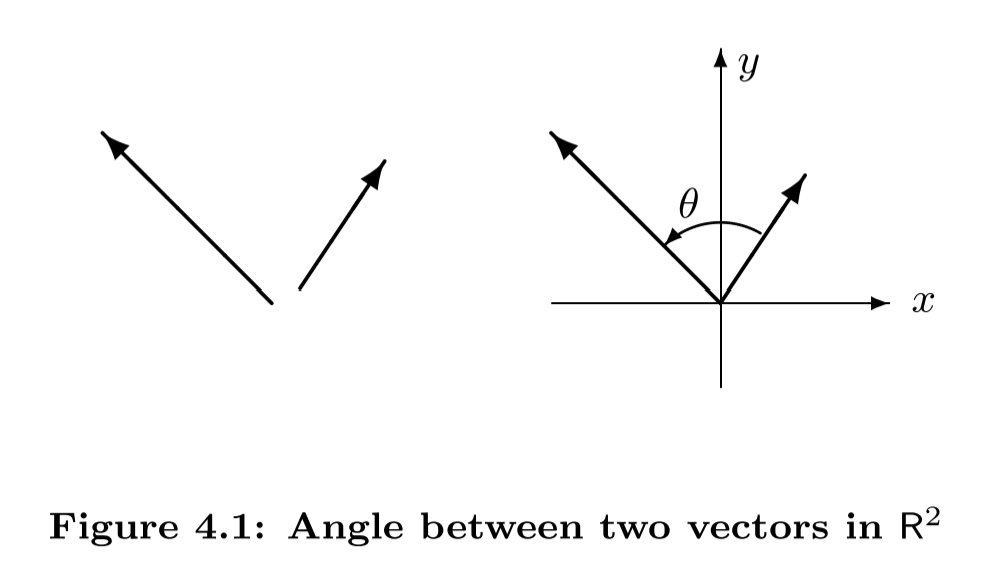
\includegraphics[width=12cm]{images/figure-4-1.png}

If \(\beta = \{ u, v \}\) is an ordered basis for \(\SET{R}^2\), we define the \textbf{orientation} of \(\beta\) to be the \emph{real number}
\[
    \mathcal{O} \begin{pmatrix} u \\ v \end{pmatrix}
    = \frac {\det\begin{pmatrix} u \\ v \end{pmatrix}} {\left| \det\begin{pmatrix} u \\ v \end{pmatrix} \right| }.
\]
(The denominator of this fraction is nonzero by \THM{4.2}.)
Clearly,
\[
    \mathcal{O} \begin{pmatrix} u \\ v \end{pmatrix} = \pm 1.
\]
\end{additional definition}

\begin{additional definition} \label{adef 4.2}
Notice that
\[
    \mathcal{O} \begin{pmatrix} e_1 \\ e_2 \end{pmatrix} = 1.
    \text{ and }
    \mathcal{O} \begin{pmatrix} e_1 \\ \RED{-e_2} \end{pmatrix} = -1.
\]
Recall that a coordinate system \(\{ u, v \}\) is called \textbf{right-handed} if \(u\) can be \emph{rotated in a counterclockwise} direction through an angle \(\theta\) \((0 < \theta < \pi\))to coincide with \(v\).
Otherwise \(\{ u, v \}\) is called a \textbf{left-handed system}.
(See Figure 4.2.)

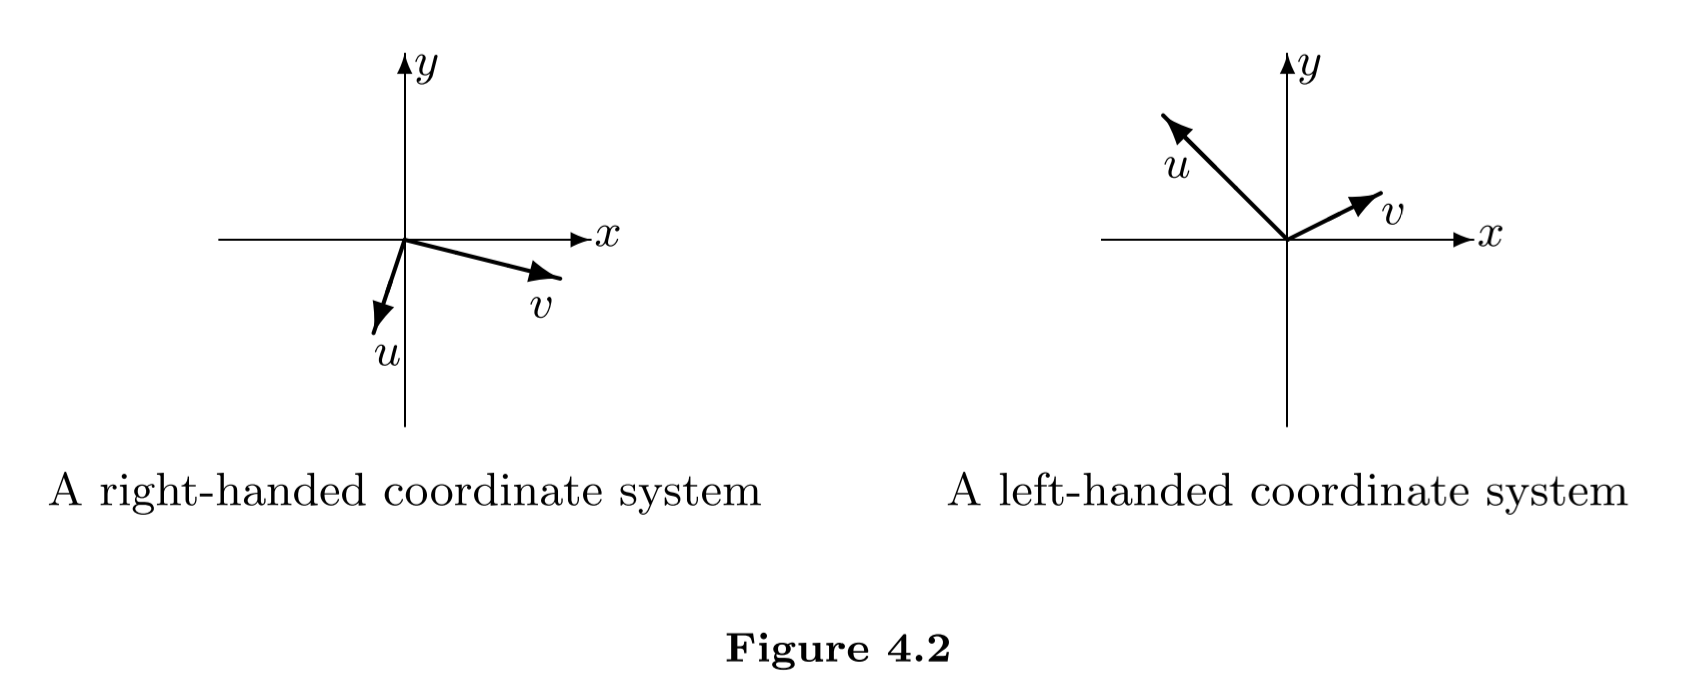
\includegraphics[width=16cm]{images/figure-4-2.png}

In general (see \EXEC{4.1.13}),
\[
    \mathcal{O} \begin{pmatrix} u \\ v \end{pmatrix} = 1.
\]
if and only if the ordered basis \(\{ u, v \}\) forms a right-banded coordinate system.
\end{additional definition}

\begin{remark} \label{remark 4.1.3}
For convenience, we also define
\[
    \mathcal{O} \begin{pmatrix} u \\ v \end{pmatrix} = 1.
\]
if \(\{ u, v \}\) is linearly \textbf{dependent}.
\end{remark}

Any ordered set \(\{ u, v \}\) in \(\SET{R}^2\) determines a parallelogram in the following manner.
Regarding \(u\) and \(v\) as arrows emanating from the origin of \(\SET{R}^2\), we call the \textbf{parallelogram} having \(u\) and \(v\) as \emph{adjacent sides} the \textbf{parallelogram
determined by \(u\) and \(v\)}.
(See Figure 4.3.)

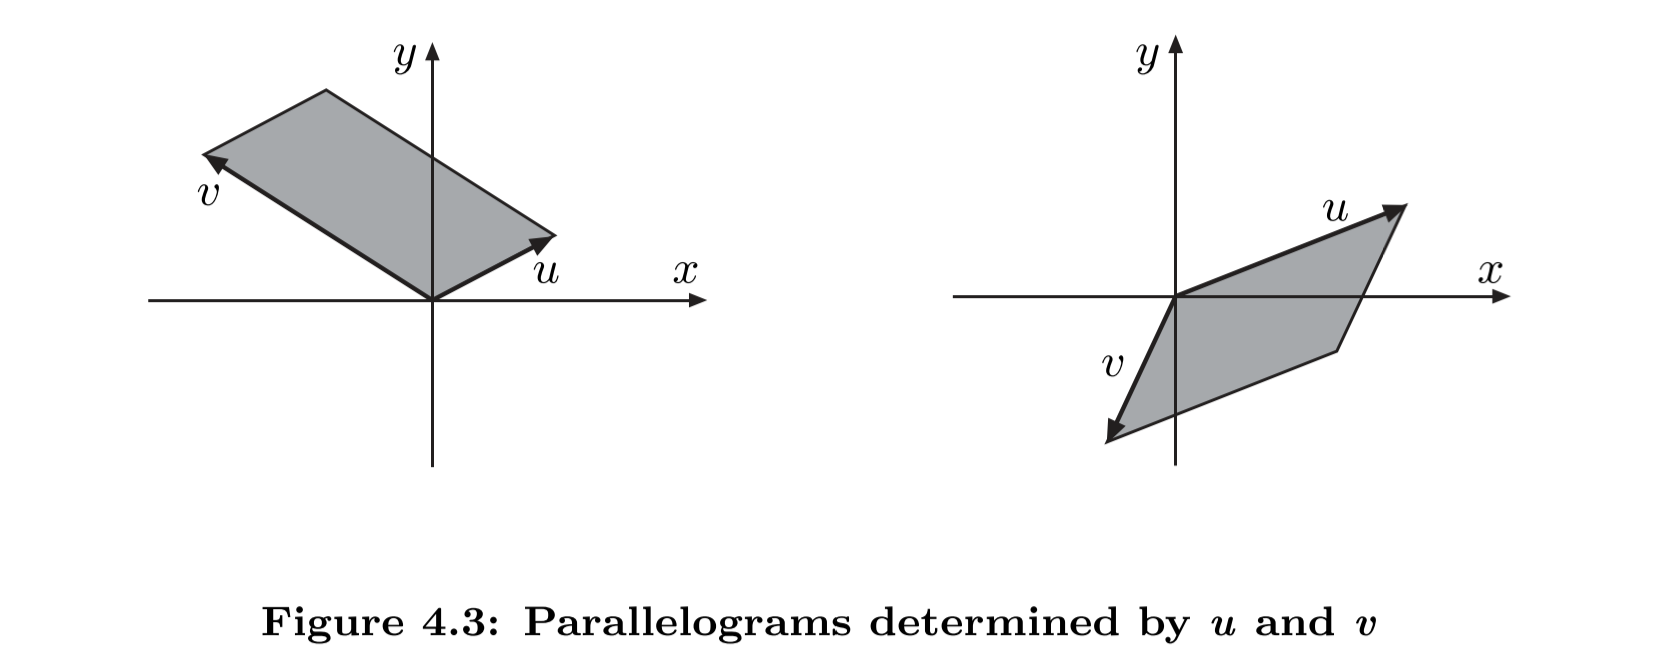
\includegraphics[width=16cm]{images/figure-4-3.png}

\begin{remark} \label{remark 4.1.4}
Observe that if the set \(\{ u, v \}\) is linearly \textbf{dependent} (i.e., if \(u\) and \(v\) are \emph{parallel}),
then the ``parallelogram'' determined by \(u\) and \(v\) is \emph{actually a line segment}, which we consider to be a
\href{https://www.wikiwand.com/en/Degeneracy_(mathematics)}{\textbf{degenerate}} parallelogram having area zero.
\end{remark}

\begin{additional theorem} \label{athm 4.1}
We have
\[
    \mathcal{A}\begin{pmatrix} u \\ v \end{pmatrix}
    = \left| \det \begin{pmatrix} u \\ v \end{pmatrix} \right|.
\]
Where \(\mathcal{A}\begin{pmatrix} u \\ v \end{pmatrix}\) denotes the area of the parallelogram determined by \(u\) and \(v\).
The proof is in the long and messy discussion below.
\end{additional theorem}

\begin{proof}
Since
\[
    \det \begin{pmatrix} u \\ v \end{pmatrix}
\]
may be negative, we cannot expect that
\[
    \mathcal{A}\begin{pmatrix} u \\ v \end{pmatrix} = \det \begin{pmatrix} u \\ v \end{pmatrix}.
\]
But \textbf{we can prove that}
\begin{equation} \label{area.formula}
    \mathcal{A}\begin{pmatrix} u \\ v \end{pmatrix} = \mathcal{O}\begin{pmatrix} u \\ v \end{pmatrix} \cdot \det \begin{pmatrix} u \\ v \end{pmatrix}
\end{equation}
from which it clearly follows that
\begin{equation} \label{simplified.area.formula}
    \mathcal{A}\begin{pmatrix} u \\ v \end{pmatrix} = \left| \det \begin{pmatrix} u \\ v \end{pmatrix} \right|.
\end{equation}
Our argument that \ref{area.formula} is correct employs a technique that, although somewhat indirect, can be \emph{generalized to \(\SET{R}^n\)}.
(Hence we will employ a similar argument in \SEC{4.2} and \SEC{4.3}.)

First, since
\[
    \mathcal{O} \begin{pmatrix} u \\ v \end{pmatrix} = \pm 1,
\]
we may multiply both sides of \ref{area.formula} by
\[
    \mathcal{O} \begin{pmatrix} u \\ v \end{pmatrix}
\]
to obtain the equivalent form
\[
    \mathcal{O}\begin{pmatrix} u \\ v \end{pmatrix} \mathcal{A}\begin{pmatrix} u \\ v \end{pmatrix} = \left(\mathcal{O}\begin{pmatrix} u \\ v \end{pmatrix}\right)^2 \cdot \det \begin{pmatrix} u \\ v \end{pmatrix} =
    1 \cdot \det \begin{pmatrix} u \\ v \end{pmatrix} =
    \det \begin{pmatrix} u \\ v \end{pmatrix},
\]
that is,
\begin{equation} \label{equivalent.area.formula}
    \det \begin{pmatrix} u \\ v \end{pmatrix}
    = \mathcal{O}\begin{pmatrix} u \\ v \end{pmatrix} \mathcal{A}\begin{pmatrix} u \\ v \end{pmatrix}.
\end{equation}
Hence \ref{equivalent.area.formula} is true if and only if \ref{area.formula} is true.
So we prove \ref{equivalent.area.formula} instead.

But first we \textbf{define} the function
\begin{equation} \label{def.delta}
    \delta \begin{pmatrix} u \\ v \end{pmatrix}
    = \mathcal{O}\begin{pmatrix} u \\ v \end{pmatrix}
      \cdot \mathcal{A}\begin{pmatrix} u \\ v \end{pmatrix}.
\end{equation}
And we will verify that \ref{def.delta} satisfies the three conditions of \EXEC{4.1.11}, and hence by \EXEC{4.1.11}, \(\delta\) is actually equal to \(\det\);
that is, \ref{equivalent.area.formula} is correct. (hence \ref{area.formula} is correct.)

\begin{note}
I recommend read \EXEC{4.1.11} first and go back to this very long and messy proof.
\end{note}

So we prove that \(\delta\) satisfies the three conditions in \EXEC{4.1.11} below:
\begin{enumerate}
\item For the first condition in \EXEC{4.1.11}, we need to show the four equations(given appropriate \(u, v, u_1, u_2, v_1, v_2, c\)):
\begin{align*}
    \delta \begin{pmatrix} u \\ cv \end{pmatrix}
    & = c \cdot \delta \begin{pmatrix} u \\ v \end{pmatrix} \\
    \delta \begin{pmatrix} cu \\ v \end{pmatrix}
    & = c \cdot \delta \begin{pmatrix} u \\ v \end{pmatrix} \\
    \delta \begin{pmatrix} u \\ v_1 + v_2 \end{pmatrix}
    & = \delta \begin{pmatrix} u \\ v_1 \end{pmatrix}
      + \delta \begin{pmatrix} u \\ v_2 \end{pmatrix} \\
    \delta \begin{pmatrix} u_1 + u_2 \\ v \end{pmatrix}
    & = \delta \begin{pmatrix} u_1 \\ v \end{pmatrix}
      + \delta \begin{pmatrix} u_2 \\ v \end{pmatrix}
\end{align*}
We begin by showing that for any real number \(c\)
\[
    \delta \begin{pmatrix} u \\ cv \end{pmatrix}
    = c \cdot \delta \begin{pmatrix} u \\ v \end{pmatrix}.
\]
Observe that this equation is valid if \(c = 0\) because
\begin{align*}
    \delta \begin{pmatrix} u \\ cv \end{pmatrix}
        & = \delta \begin{pmatrix} u \\ 0 \end{pmatrix} & \text{of course} \\
        & = \mathcal{O}\begin{pmatrix} u \\ 0 \end{pmatrix} \cdot \mathcal{A}\begin{pmatrix} u \\ v \end{pmatrix} & \text{by def in \ref{def.delta}} \\
        & = 1 \cdot \mathcal{A}\begin{pmatrix} u \\ v \end{pmatrix} & \text{by \RMK{4.1.3}} \\
        & = 1 \cdot 0 & \text{by \RMK{4.1.4}} \\
        & = 0 & \text{of course} \\
        & = 0 \cdot \delta \begin{pmatrix} u \\ v \end{pmatrix} & \text{of course} \\
        & = c \cdot \delta \begin{pmatrix} u \\ v \end{pmatrix}.
\end{align*}
So assume that \(c \ne 0\).
Regarding \(cv\) as the \emph{base of the parallelogram} determined by \(u\) and \(cv\), (by geometry formula) we see that
\begin{align*}
    \mathcal{A}\begin{pmatrix}
        u \\ cv
    \end{pmatrix}
    & = \text{(base of \(cv\) and \(u\))} \X \text{(altitude of \(cv\) and \(u\))} & \text{by geometry formula} \\
    & = \abs{c} \cdot (\text{length of } v) \X (\text{altitude of \(cv\) and \(u\)}) \\
    & = \abs{c} \cdot (\text{length of } v) \X (\text{altitude \textbf{of \(v\) and \(u\)}}) \\
    & \text{\ \ \ \ \ \ (since the altitude of these parallelograms are)} \\
    & \text{\ \ \ \ \ \ (the same; see Figure 4.4.)} \\
    & = \abs{c} \mathcal{A}\begin{pmatrix}
        u \\ v
    \end{pmatrix}. & \text{by geometry formula}
\end{align*}
So we have
\[
    \mathcal{A}\begin{pmatrix}
        u \\ cv
    \end{pmatrix}
    = \abs{c} \mathcal{A}\begin{pmatrix}
        u \\ v
    \end{pmatrix}. \text{ -- \MAROON{(a.1)}}
\]

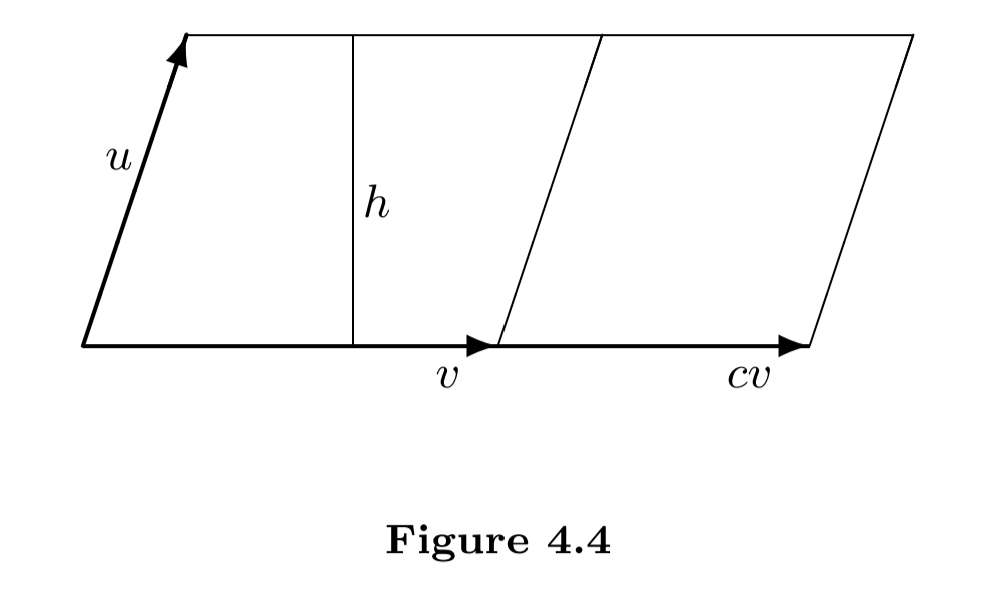
\includegraphics[width=10cm]{images/figure-4-4.png}

Hence
\begin{align*}
    \delta \begin{pmatrix}
        u \\ cv
    \end{pmatrix}
    & = \mathcal{O}\begin{pmatrix} u \\ cv \end{pmatrix} \cdot \mathcal{A}\begin{pmatrix} u \\ cv \end{pmatrix} & \text{by def in \ref{def.delta}} \\
    & = \left[\frac{c}{\abs{c}} \mathcal{O}\begin{pmatrix} u \\ v \end{pmatrix}\right] \mathcal{A}\begin{pmatrix} u \\ cv \end{pmatrix} & \text{need to prove but trivial by def of \(\mathcal{O}\)} \\
    & = \left[\frac{c}{\abs{c}} \mathcal{O}\begin{pmatrix} u \\ v \end{pmatrix}\right] \left[\abs{c} \mathcal{A}\begin{pmatrix} u \\ v \end{pmatrix}\right] & \text{by \MAROON{(a.1)}} \\
    & = c \cdot \mathcal{O}\begin{pmatrix} u \\ v \end{pmatrix} \cdot \mathcal{A}\begin{pmatrix} u \\ v \end{pmatrix} & \text{of course} \\
    & = c \cdot \delta \begin{pmatrix}
        u \\ v
    \end{pmatrix}. & \text{by def in \ref{def.delta}}
\end{align*}
A similar argument shows
\[
    \delta \begin{pmatrix}
        cu \\ v
    \end{pmatrix}
    = c \cdot \delta \begin{pmatrix}
        u \\ v
    \end{pmatrix}.
\]

So currently we have shown that
\[
    \delta \begin{pmatrix}
        u \\ cv
    \end{pmatrix}
    = c \cdot \delta \begin{pmatrix}
        u \\ v
    \end{pmatrix}.
    \text{ and }
    \delta \begin{pmatrix}
        cu \\ v
    \end{pmatrix}
    = c \cdot \delta \begin{pmatrix}
        u \\ v
    \end{pmatrix}. \text{ -- \BLUE{(1)}}
\]

Now before we prove the remaining two equations, we first prove that
\[
    \delta \begin{pmatrix}
        u \\ a\RED{u} + bw
    \end{pmatrix}
    = b \cdot \delta \begin{pmatrix}
        u \\ w
    \end{pmatrix}
\]
for any \(u, w \in \SET{R}^2\).
Because the parallelograms determined by \(u\) and \(w\) and by \(u\) and \(u + w\) \emph{have a common base} \(u\) and the same altitude (see Figure 4.5), (by geometry) it follows that
\[
    \mathcal{A} \begin{pmatrix}
        u \\ w
    \end{pmatrix}
    = \mathcal{A} \begin{pmatrix}
        u \\ \RED{u} + w
    \end{pmatrix}
\]
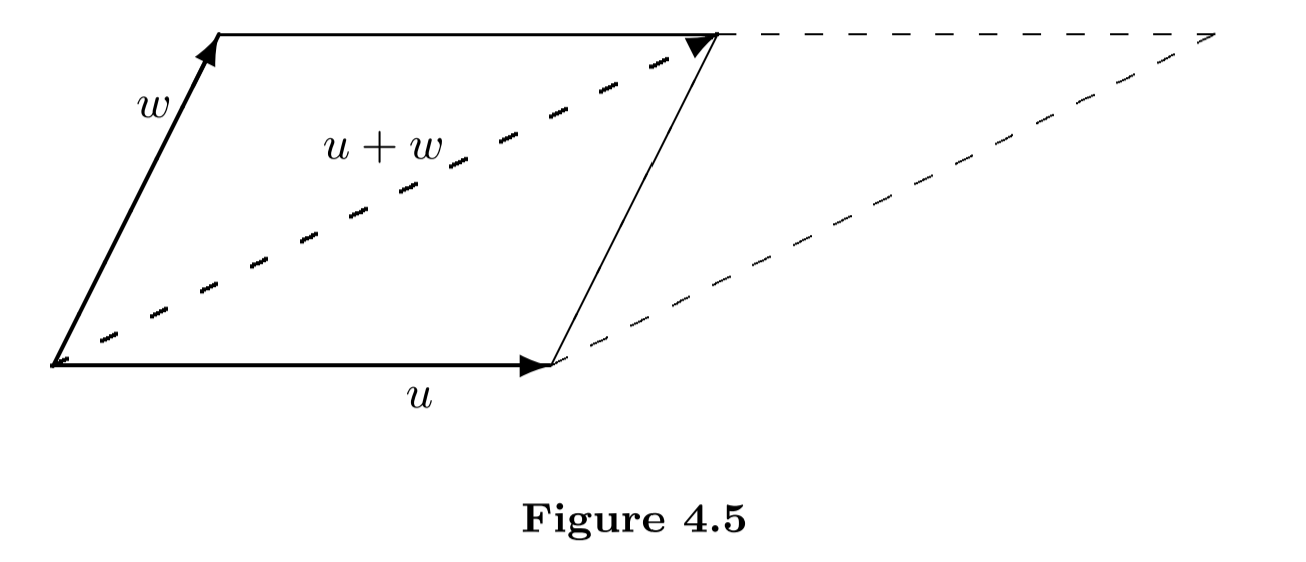
\includegraphics[width=14cm]{images/figure-4-5.png}

If \(a = 0\), then
\begin{align*}
    \delta \begin{pmatrix} u \\ au + bw \end{pmatrix}
    = \delta \begin{pmatrix} u \\ 0 + bw \end{pmatrix}
    & = \delta \begin{pmatrix} u \\ bw \end{pmatrix} \\
    & = b \cdot \delta \begin{pmatrix} u \\ w \end{pmatrix}. & \text{by \BLUE{(1)}}
\end{align*}
Otherwise, if \(a \ne 0\), then
\begin{align*}
    \delta \begin{pmatrix}
        u \\ au + bw
    \end{pmatrix}
    & = \delta \begin{pmatrix}
        u \\ a(u + \frac{b}{a}w)
    \end{pmatrix} & \text{of course} \\
    & = a \cdot \delta \begin{pmatrix}
        u \\ u + \frac{b}{a}w
    \end{pmatrix} & \text{by \BLUE{(1)}} \\
    & = a \cdot \delta \begin{pmatrix}
        u \\ \frac{b}{a}w
    \end{pmatrix} & \text{(indirectly) by Figure 4.5} \\
    & = a \left( \frac{b}{a} \right) \cdot \delta \begin{pmatrix}
        u \\ w
    \end{pmatrix} & \text{by \BLUE{(1)} again} \\
    & = b \cdot \delta \begin{pmatrix}
        u \\ w
    \end{pmatrix} & \text{of course}.
\end{align*}
So in all cases, we have
\[
    \delta \begin{pmatrix}
        u \\ au + bw
    \end{pmatrix}
    = b \cdot \delta \begin{pmatrix}
        u \\ w
    \end{pmatrix}. \text{ -- \BLUE{(2)}}
\]
Finally, we now are able to show that
\[
    \delta \begin{pmatrix}
        u \\ v_1 + v_2
    \end{pmatrix}
    = \delta \begin{pmatrix}
        u \\ v_1
    \end{pmatrix}
    + \delta \begin{pmatrix}
        u \\ v_2
    \end{pmatrix}
\]
for all \(u, v_1, v_2 \in \SET{R}^2\).
Since the result is immediate if \(u = 0\)
(that will cause every term to be zero, since the area of the corresponding parallelogram will we zero),
we assume that \(u \ne 0\).
Choose any vector \(w \in \SET{R}^2\) such that \(\{ u, w \}\) is \emph{\LID{}}.
Then for any vectors \(v_1, v_2 \in \SET{R}^2\) there exist (unique) scalars \(a_i\) and \(b_i\) such that
\[
    v_i = a_i u + b_i w \ \  (i = 1, 2). \text{ -- \MAROON{(a.2)}}
\]
Thus
\begin{align*}
    \delta \begin{pmatrix}
        u \\ v_1 + v_2
    \end{pmatrix}
    & = \delta \begin{pmatrix}
            u \\ (a_1 + a_2) \RED{u} + (b_1 + b_2) w
        \end{pmatrix} & \text{by \MAROON{(a.2)}} \\
    & = (b_1 + b_2) \delta \begin{pmatrix}
            u \\ w
        \end{pmatrix} & \text{by \BLUE{(2)}} \\
    & = b_1 \delta \begin{pmatrix}
            u \\ w
        \end{pmatrix}
      + b_2 \delta \begin{pmatrix}
            u \\ w
        \end{pmatrix} & \text{of course} \\
    & = \delta \begin{pmatrix}
            u \\ a_1 u + b_1 w
        \end{pmatrix}
      + \delta \begin{pmatrix}
            u \\ a_2 u + b_2 w
        \end{pmatrix} & \text{again by \BLUE{(2)}} \\
    & = \delta \begin{pmatrix}
            u \\ v_1
        \end{pmatrix}
      + \delta \begin{pmatrix}
            u \\ v_2
        \end{pmatrix} & \text{by \MAROON{(a.2)}}
\end{align*}
A similar argument shows that
\[
    \delta \begin{pmatrix}
        u_1 + u_2 \\ v
    \end{pmatrix}
    = \delta \begin{pmatrix}
            u_1 \\ v
        \end{pmatrix}
      + \delta \begin{pmatrix}
            u_2 \\ v
        \end{pmatrix}
\]
for all \(u_1, u_2, v \in \SET{R}^2\).

So finally, we have proved that the four equations in the first condition of \EXEC{4.1.11} are satisfied by definition of \(\delta\) in \ref{def.delta}.

\item
Since (by geometry) \(\mathcal{A} \begin{pmatrix} u \\ u \end{pmatrix} = 0\), it follows that
\begin{align*}
    \delta \begin{pmatrix} u \\ u \end{pmatrix}
    & = \mathcal{O} \begin{pmatrix} u \\ u \end{pmatrix} \cdot \mathcal{A} \begin{pmatrix} u \\ u \end{pmatrix} & \text{by def in \ref{def.delta}} \\
    & = 0
\end{align*}
for any \(u \in \SET{R}^2\).

\item
Because (by geometry) the parallelogram determined by \(e_1\) and \(e_2\) is the \emph{unit square},
\begin{align*}
    \delta(I_2)
    & = \delta \begin{pmatrix} e_1 \\ e_2 \end{pmatrix} \\
    & = \mathcal{O} \begin{pmatrix} e_1 \\ e_2 \end{pmatrix} \cdot \mathcal{A} \begin{pmatrix} e_1 \\ e_2 \end{pmatrix} & \text{by def in \ref{def.delta}} \\
    & = 1 \cdot \mathcal{A} \begin{pmatrix} e_1 \\ e_2 \end{pmatrix} & \text{of course (by calculation)} \\
    & = 1 \cdot 1 & \text{since the parallelogram is the unit square} \\
    & = 1.
\end{align*}
\end{enumerate}

Therefore, \(\delta\) defined in \ref{def.delta} satisfies the three conditions of \EXEC{4.1.11}, and hence \(\delta = \det\).
Hence \ref{equivalent.area.formula}, \ref{area.formula} and \ref{simplified.area.formula} are correct;
that is,
\[
    \mathcal{A}\begin{pmatrix} u \\ v \end{pmatrix}
    = \mathcal{O}\begin{pmatrix} u \\ v \end{pmatrix} \cdot \det \begin{pmatrix} u \\ v \end{pmatrix}
    = \left| \det \begin{pmatrix} u \\ v \end{pmatrix} \right|.
\]
\end{proof}

Thus we see, for example, that the area of the parallelogram determined by \(u = (-1, 5)\) and \(v = (4, -2)\) is
\[
    \left| \det \begin{pmatrix}
        u \\ v
    \end{pmatrix} \right|
    = \left| \det \begin{pmatrix}
        -1 & 5 \\ 4 & -2
    \end{pmatrix} \right|
    = 18.
\]

\exercisesection

\begin{exercise} \label{exercise 4.1.1}
Label the following statements as true or false.
\begin{enumerate}
\item The function \(\det : M_{2 \X 2}(F) \to F\) is a linear transformation.
\item The determinant of a \(2 \X 2\) matrix is a linear function of each row of the matrix when the other row is held fixed.
\item If \(A \in M_{2 \X 2}(F)\) and \(\det(A) = 0\), then \(A\) is invertible.
\item If \(u\) and \(v\) are vectors in \(\SET{R}^2\) emanating from the origin, then the area of the parallelogram having \(u\) and \(v\) as adjacent sides is
\[
    \det \begin{pmatrix} u \\ v \end{pmatrix}.
\]
\item A coordinate system is \emph{right-handed} if and only if its orientation equals \(1\).
\end{enumerate}
\end{exercise}

\begin{proof} \ 

\begin{enumerate}
\item False by \RMK{4.1.1}.
\item True by \THM{4.1}.
\item False, by \THM{4.2}, \(A\) is \emph{not} invertible.
\item False, by \ATHM{4.1}, the areas is
\[
    \left| \det \begin{pmatrix} u \\ v \end{pmatrix} \right|.
\]
\item True by \EXEC{4.1.13}.
\end{enumerate}
\end{proof}

\begin{exercise} \label{exercise 4.1.2}
Compute the determinants of the following matrices in  \(M_{2 \X 2}(\SET{R})\).

(a) \(\left(\begin{array}{rr} 6 & -3 \\ 2 & 4 \end{array}\right)\)
(b) \(\left(\begin{array}{rr} -5 & 2 \\ 6 & 1 \end{array}\right)\)
(c) \(\left(\begin{array}{rr} 8 & 0 \\ 3 & -1 \end{array}\right)\)
\end{exercise}

\begin{proof} \ 

\begin{enumerate}
\item
\[
    \det \left(\begin{array}{rr} 6 & -3 \\ 2 & 4 \end{array}\right) = 6 \cdot 4 - (-3) \cdot 2 = 30.
\]
\item
\[
    \det \left(\begin{array}{rr} -5 & 2 \\ 6 & 1 \end{array}\right) = -5 \cdot 1 - 2 \cdot 6 = -17.
\]
\item
\[
    \det \left(\begin{array}{rr} 8 & 0 \\ 3 & -1 \end{array}\right) = 8 \cdot (-1) - 0 \cdot 3 = -8.
\]
\end{enumerate}
\end{proof}

\begin{exercise} \label{exercise 4.1.3}
Compute the determinants of the following matrices in  \(M_{2 \X 2}(\SET{C})\).

(a) \(\left(\begin{array}{rr} -1 + \iu & 1 - 4\iu \\ 3 + 2\iu & 2 - 3\iu \end{array}\right)\)
(b) \(\left(\begin{array}{rc} 5 - 2\iu & 6 + 4\iu \\ -3 + \iu & 7\iu \end{array}\right)\)
(c) \(\left(\begin{array}{rr} 2\iu & 3 \\ 4 & 6\iu \end{array}\right)\)
\end{exercise}

\begin{proof} \ 

\begin{enumerate}
\item
\[
    \det \left(\begin{array}{rr} -1 + \iu & 1 - 4\iu \\ 3 + 2\iu & 2 - 3\iu \end{array}\right)
    = (-1 + \iu) \cdot (2 - 3\iu) - (1 - 4\iu) \cdot (3 + 2\iu)
    = -10 + 15\iu.
\]
\item
\[
    \det \left(\begin{array}{rc} 5 - 2\iu & 6 + 4\iu \\ -3 + \iu & 7\iu \end{array}\right)
    = (5 - 2\iu) \cdot (7\iu) - (6 + 4\iu) \cdot (-3 + \iu)
    = -8 + 29\iu.
\]
\item
\[
    \det \left(\begin{array}{rr} 2\iu & 3 \\ 4 & 6\iu \end{array}\right)
    = 2\iu \cdot 6\iu - 3 \cdot 4
    = -24.
\]
\end{enumerate}
\end{proof}

\begin{exercise} \label{exercise 4.1.4}
For each of the following pairs of vectors \(u\) and \(v\) in \(\SET{R}^2\), compute the area of the parallelogram determined by \(u\) and \(v\).
\begin{enumerate}
\item \(u = (3, -2)\) and \(v = (2, 5)\).
\item \(u = (1, 3)\) and \(v = (-3, 1)\).
\item \(u = (4, -1)\) and \(v = (-6, -2)\).
\item \(u = (3, 4)\) and \(v = (2, -6)\).
\end{enumerate}
\end{exercise}

\begin{proof} \ 

\begin{enumerate}
\item
\[
    \left| \det \begin{pmatrix} 3 & -2 \\ 2 & 5
\end{pmatrix} \right| = |3 \cdot 5 - (-2) \cdot 2| = 19.
\]

\item
\[
    \left| \det \begin{pmatrix} 1 & 3 \\ -3 & 1
\end{pmatrix} \right| = |1 \cdot 1 - 3 \cdot (-3)| = 10.
\]

\item
\[
    \left| \det \begin{pmatrix} 4 & -1 \\ -6 & -2
\end{pmatrix} \right| = |4 \cdot (-2) - (-1) \cdot (-6)| = 14.
\]

\item
\[
    \left| \det \begin{pmatrix} 3 & 4 \\ 2 & -6
\end{pmatrix} \right| = |3 \cdot (-6) - 4 \cdot 2| = 26.
\]
\end{enumerate}
\end{proof}

\begin{exercise} \label{exercise 4.1.5}
Prove that if \(B\) is the matrix obtained by \emph{interchanging} the rows of a \(2 \X 2\) matrix \(A\), then \(\det(B) = -\det(A)\).
\end{exercise}

\begin{proof}
Let
\[
    A = \begin{pmatrix} A_{11} & A_{12} \\ A_{21} & A_{22} \end{pmatrix}
    \text{, then }
    B = \begin{pmatrix} A_{21} & A_{22} \\ A_{11} & A_{12} \end{pmatrix}.
\]
So by \DEF{4.1}, \(\det(A) = A_{11} A_{22} - A_{12} A_{21}\), and \(\det(B) = A_{21} A_{12} - A_{22} A_{11} = A_{12} A_{21} - A_{11} A_{22} = -(A_{11} A_{22} - A_{12} A_{21}) = -\det(A)\), as desired.
\end{proof}

\begin{exercise} \label{exercise 4.1.6}
Prove that if the two \emph{columns} of \(A \in M_{2 \X 2}(F)\) are identical, then \(\det(A) = 0\).
\end{exercise}

\begin{proof}
If columns of \(A\) are identical, then (by \CH{3}) \(A\) is not invertible, and by \THM{4.2}, \(\det(A) = 0\).
\end{proof}

\begin{exercise} \label{exercise 4.1.7}
Prove that \(\det(A^\top) = \det(A)\) for any \(A \in M_{2 \X 2}(F)\).
\end{exercise}

\begin{proof}
Let
\[
    A = \begin{pmatrix} A_{11} & A_{12} \\ A_{21} & A_{22} \end{pmatrix}
\]
then
\[
    A^\top = \begin{pmatrix} A_{11} & A_{21} \\ A_{12} & A_{22} \end{pmatrix}
\]
So by \DEF{4.1}, \(\det(A) = A_{11} A_{22} - A_{12} A_{21}\), and \(\det(A^\top) = A_{11} A_{22} - A_{21} A_{12} = A_{11} A_{22} - A_{12} A_{21} = \det(A)\), as desired.
\end{proof}

\begin{exercise} \label{exercise 4.1.8}
Prove that if \(A \in M_{2 \X 2}(F)\) is \emph{upper triangular}, then \(\det(A)\) equals the \emph{product of the diagonal} entries of \(A\).
\end{exercise}

\begin{proof}
Since \(A\) is upper triangular, \(A\) has the form
\[
    A^\top = \begin{pmatrix} A_{11} & A_{12} \\ \RED{0} & A_{22} \end{pmatrix}
\]
And by \DEF{4.1}, \(\det(A) = A_{11} A_{22} - A_{12} \cdot 0 = A_{11} A_{22}\), which is the product of the diagonal entries of \(A\).
\end{proof}

\begin{exercise} \label{exercise 4.1.9}
Prove that \(\det(AB) = \det(A) \cdot \det(B)\) for any \(A, B \in M_{2 \X 2}(F)\).
\end{exercise}

\begin{proof}
Let
\[
    A = \begin{pmatrix} a_1 & a_2 \\ a_3 & a_4 \end{pmatrix},
    B = \begin{pmatrix} b_1 & b_2 \\ b_3 & b_4 \end{pmatrix}.
\]
Then (by calculation)
\[
    AB = \begin{pmatrix}
        a_1 b_1 + a_2 b_3 & a_1 b_2 + a_2 b_4 \\
        a_3 b_1 + a_4 b_3 & a_3 b_2 + a_4 b_4
    \end{pmatrix}.
\]
So by \DEF{4.1},
\begin{align*}
    \det(A) & = a_1 a_4 - a_2 a_3, \\
    \det(B) & = b_1 b_4 - b_2 b_3, \\
    \det(A)\det(B) & = (a_1 a_4 - a_2 a_3)(b_1 b_4 - b_2 b_3) \\
                   & = (a_1 a_4 b_1 b_4 - a_1 a_4 b_2 b_3 - a_2 a_3 b_1 b_4 + a_2 a_3 b_2 b_3) \text{ -- \MAROON{(1)}}, \\
    \det(AB) & = (a_1 b_1 + a_2 b_3)(a_3 b_2 + a_4 b_4) - (a_1 b_2 + a_2 b_4)(a_3 b_1 + a_4 b_3) \\
             & = (\GREEN{a_1 b_1 a_3 b_2} + a_1 b_1 a_4 b_4 + a_2 b_3 a_3 b_2 + \BLUE{a_2 b_3 a_4 b_4}) \\
             & \ \ \ \  \RED{-} (\GREEN{a_1 b_2 a_3 b_1} + a_1 b_2 a_4 b_3 + a_2 b_4 a_3 b_1 + \BLUE{a_2 b_4 a_4 b_3}) \\
             & = (a_1 b_1 a_4 b_4 + a_2 b_3 a_3 b_2) - (a_1 b_2 a_4 b_3 + a_2 b_4 a_3 b_1) \\
             & = (a_1 a_4 b_1 b_4 + a_2 a_3 b_2 b_3) - (a_1 a_4 b_2 b_3 + a_2 a_3 b_1 b_4) \\
             & = \MAROON{(1)} = \det(A)\det(B),
\end{align*}
as desired.
\end{proof}

\begin{exercise} \label{exercise 4.1.10}
The \textbf{classical adjoint} of a \(2 \X 2\) matrix \(A \in M_{2 \X 2}(F)\) is the matrix
\[
    C = \begin{pmatrix} A_{22} & -A_{12} \\ -A_{21} & A_{11} \end{pmatrix}.
\]
Prove that
\begin{enumerate}
\item \(CA = AC = [\det(A)]I\).
\item \(\det(C) = \det(A)\).
\item The classical adjoint of \(A^\top\) is \(C^\top\).
\item If \(A\) is invertible, then \(A^{-1} = [\det(A)]^{-1}C\).
\end{enumerate}
\end{exercise}

\begin{proof} \ 

\begin{enumerate}
\item
\begin{align*}
    AC & =
        \begin{pmatrix}
            A_{11} & A_{12} \\
            A_{21} & A_{22}
        \end{pmatrix}
        \begin{pmatrix}
            A_{22} & -A_{12} \\
            -A_{21} & A_{11}
        \end{pmatrix} \\
      & = \begin{pmatrix}
            A_{11} A_{22} - A_{12} A_{21} & -A_{11} A_{12} + A_{12} A_{11} \\
            A_{21} A_{22} - A_{22} A_{21} & - A_{21} A_{12} + A_{22} A_{11}
        \end{pmatrix}
      & = \begin{pmatrix}
          \det(A) & 0 \\
          0 & \det(A)
      \end{pmatrix}
      & = \det(A) \cdot I_2.
\end{align*}
and
\begin{align*}
   CA & =
        \begin{pmatrix}
            A_{22} & -A_{12} \\
            -A_{21} & A_{11}
        \end{pmatrix}
        \begin{pmatrix}
            A_{11} & A_{12} \\
            A_{21} & A_{22}
        \end{pmatrix} \\
      & = \begin{pmatrix}
            A_{22} A_{11} - A_{12} A_{21} & A_{22} A_{12} - A_{12} A_{22} \\
            -A_{21} A_{11} + A_{11} A_{21} & - A_{21} A_{12} + A_{11} A_{22}
        \end{pmatrix}
      & = \begin{pmatrix}
          \det(A) & 0 \\
          0 & \det(A)
      \end{pmatrix}
      & = \det(A) \cdot I_2. 
\end{align*}

\item
We have
\[
    \det(C) = A_{22}A_{11} - (-A_{12})(-A_{21}) = A_{22} A_{11} - A_{12} A_{21} = \det(A).
\]

\item First,
\[
    A^\top = \begin{pmatrix}
        A_{11} & A_{21} \\
        A_{12} & A_{22}
    \end{pmatrix}
\]
so by def, the adjoint matrix of \(A^\top\) is
\[
    \begin{pmatrix}
        A_{22}^\top & -A_{12}^\top \\
        -A_{21}^\top & A_{11}^\top    
    \end{pmatrix}
\]
which by definition of transpose (of each entry) is
\[
    \begin{pmatrix}
        A_{22} & -A_{21} \\
        -A_{12} & A_{11}
    \end{pmatrix}
\]
which by definition of transpose again is \(C^\top\).

\item
We have
\begin{align*}
    A ([\det(A)]^{-1} C)
    & = [\det(A)]^{-1} (AC) & \text{of course, or by \THM{2.12}(b)} \\
    & = [\det(A)]^{-1} [\det(A)] I & \text{by part(a)} \\
    & = I.
\end{align*}
And by \ATHM{2.38}, ``one-sided'' inverse is a ``two-sided'' inverse, we have \(A^{-1} = [\det(A)]^{-1} C\).
\end{enumerate}
\end{proof}

\begin{exercise} \label{exercise 4.1.11}
Let \(\delta: M_{2 \X 2}(F) \to F\) be a function with the following three properties.
\begin{enumerate}
\item[(i)] \(\delta\) is a linear function of each row of the matrix when the other row is held fixed.
\item[(ii)] If the two rows of \(A \in M_{2 \X 2}(F)\) are identical, then \(\delta(A) = 0\).
\item[(iii)] If \(I\) is the \(2 \X 2\) identity matrix, then \(\delta(I) = 1\).
\end{enumerate}

Then
\begin{enumerate}
\item Prove that \(\delta(E) = \det(E)\) for all \textbf{elementary} matrices \(E \in M_{2 \X 2}(F)\).
\item Prove that \(\delta(EA) = \delta(E)\delta(A)\) for all \(A \in M_{2 \X 2}(F)\) and all \textbf{elementary} matrices \(E \in M_{2 \X 2}(F)\).
\end{enumerate}
\end{exercise}

\begin{proof} \ 

\begin{enumerate}
\item
We prove by cases of each type of elementary matrix.
For type 1, there are only one matrix:
\[
    E_1 = \begin{pmatrix}
        0 & 1 \\
        1 & 0
    \end{pmatrix}.
\]
It's clear that \(\det(E_1) = -1\).
Now by definition(ii) of \(\delta\), we have
\[
    \delta \begin{pmatrix} 1 & 0 \\ 1 & 0 \end{pmatrix}
    = \delta \begin{pmatrix} 0 & 1 \\ 0 & 1 \end{pmatrix}
    = \delta \begin{pmatrix} 1 & 1 \\ 1 & 1 \end{pmatrix}
    = 0 \text{ -- \MAROON{(1)}}
\]
Since each matrix above has identical rows respectively.
Then
\begin{align*}
    0 & = \delta \begin{pmatrix} 1 & 1 \\ 1 & 1 \end{pmatrix} & \text{by \MAROON{(1)}} \\
      & = \delta \begin{pmatrix} 1 & 0 \\ 1 & 1 \end{pmatrix}
          + \delta \begin{pmatrix} 0 & 1 \\ 1 & 1 \end{pmatrix} & \text{by def (i) of \(\delta\), fix row \(2\)} \\
      & = \left( \delta \begin{pmatrix} 1 & 0 \\ 1 & 0 \end{pmatrix} + \delta \begin{pmatrix} 1 & 0 \\ 0 & 1 \end{pmatrix} \right)
          + \delta \begin{pmatrix} 0 & 1 \\ 1 & 1 \end{pmatrix} & \text{by def (i) of \(\delta\), fix row \(1\)} \\
      & = (0 + 1) + \delta \begin{pmatrix} 0 & 1 \\ 1 & 1 \end{pmatrix} & \text{by \MAROON{(1)} and by def (iii) of \(\delta\)} \\
      & = 1 + \delta \begin{pmatrix} 0 & 1 \\ 1 & 1 \end{pmatrix} & \text{of course} \\
      & = 1 + \left( \delta \begin{pmatrix} 0 & 1 \\ 0 & 1 \end{pmatrix} + \delta \begin{pmatrix} 0 & 1 \\ 1 & 0 \end{pmatrix} \right) & \text{by def (i) of \(\delta\), fix row \(1\)} \\
      & = 1 + \left( 0 + \delta \begin{pmatrix} 0 & 1 \\ 1 & 0 \end{pmatrix} \right) & \text{by \MAROON{(1)}} \\
      & = 1 + \delta \begin{pmatrix} 0 & 1 \\ 1 & 0 \end{pmatrix} \\
      & = 1 + \delta(E_1)
\end{align*}
which implies \(\delta(E_1) = -1\) \MAROON{(a.1)}, which is equal to \(\det(E_1)\).

Now if \(E_2\) is a type 2 elementary matrix, we can represent \(E_2\) as
\[
    E_2 = \begin{pmatrix} c & 0 \\ 0 & 1
    \end{pmatrix}
    \text{ or }
    E_2 = \begin{pmatrix} 1 & 0 \\ 0 & c
    \end{pmatrix}
\]
We show the case of the first form; the second form is similar.
It's clear that \(\det(E_2) = c\).
And
\begin{align*}
    \delta(E_2) & = \delta \begin{pmatrix} c & 0 \\ 0 & 1 \end{pmatrix} \\
                & = c \delta \begin{pmatrix} 1 & 0 \\ 0 & 1 \end{pmatrix} & \text{by def (i) of \(\delta\), fix row \(2\)} \\
                & = c 1 & \text{by def (iii) of \(\delta\)} \\
                & = c = \det(E_2).
\end{align*}

Finally, if \(E_3\) is a type 3 elementary matrix, we can represent \(E_3\) as
\[
    E_2 = \begin{pmatrix} 1 & 0 \\ c & 1
    \end{pmatrix}
    \text{ or }
    E_2 = \begin{pmatrix} 1 & c \\ 0 & 1
    \end{pmatrix}
\]
We show the case of the first form; the second form is similar.
It's clear that \(\det(E_3) = 1\).
And
\begin{align*}
    \delta(E_3) & = \delta \begin{pmatrix} 1 & 0 \\ c & 1 \end{pmatrix} \\
                & = \delta \begin{pmatrix} 1 & 0 \\ c & 0 \end{pmatrix} + \delta \begin{pmatrix} 1 & 0 \\ 0 & 1 \end{pmatrix} & \text{by def (i) of \(\delta\), fix row \(1\)} \\
                & = c \delta \begin{pmatrix} 1 & 0 \\ 1 & 0 \end{pmatrix} + \delta \begin{pmatrix} 1 & 0 \\ 0 & 1 \end{pmatrix} & \text{by def (i) of \(\delta\), fix row \(1\)} \\
                & = c \cdot 0 + \delta \begin{pmatrix} 1 & 0 \\ 0 & 1 \end{pmatrix} & \text{by def (ii) of \(\delta\)} \\
                & = \delta \begin{pmatrix} 1 & 0 \\ 0 & 1 \end{pmatrix} & \text{of course} \\
                & = 1 & \text{by def (iii) of \(\delta\)} \\
                & = \det(E_3).
\end{align*}
So we have shown that \(\det(E) = \delta(E)\) for any \emph{elementary} matrix \(E\).

\item
Let arbitrary \(2 \X 2\) matrix
\[
    A = \begin{pmatrix}
        a_1 & a_2 \\ a_3 & a_4
    \end{pmatrix}.
\]
Then
\begin{align*}
    \delta(A) & = \delta \begin{pmatrix} a_1 & a_2 \\ a_3 & a_4 \end{pmatrix} \\
              & = \delta \begin{pmatrix} a_1 & a_2 \\ a_3 & 0 \end{pmatrix}
                + \delta \begin{pmatrix} a_1 & a_2 \\ 0 & a_4 \end{pmatrix} & \text{by (i), fix row \(1\)} \\
              & = \left(
                    \delta \begin{pmatrix} a_1 & 0 \\ a_3 & 0 \end{pmatrix}
                    + \delta \begin{pmatrix} 0 & a_2 \\ a_3 & 0 \end{pmatrix}
                \right)
                + \left(
                    \delta \begin{pmatrix} a_1 & 0 \\ 0 & a_4 \end{pmatrix}
                    + \delta \begin{pmatrix} 0 & a_2 \\ 0 & a_4 \end{pmatrix}
                \right) & \text{by (i), fix row \(1\)} \\
              & = a_1 a_3 \delta \begin{pmatrix} 1 & 0 \\ 1 & 0 \end{pmatrix}
                + a_2 a_3 \delta \begin{pmatrix} 0 & 1 \\ 1 & 0 \end{pmatrix}
                + a_1 a_4 \delta \begin{pmatrix} 1 & 0 \\ 0 & 1 \end{pmatrix}
                + a_2 a_4 \delta \begin{pmatrix} 0 & 1 \\ 0 & 1 \end{pmatrix} \\
              & \text{\ \ \ \ \  (by applying (i) multiple times)} \\
              & = a_1 a_3 \cdot 0
                + a_2 a_3 \delta \begin{pmatrix} 0 & 1 \\ 1 & 0 \end{pmatrix}
                + a_1 a_4 \delta \begin{pmatrix} 1 & 0 \\ 0 & 1 \end{pmatrix}
                + a_2 a_4 \cdot 0 & \text{by (ii)} \\
              & = a_2 a_3 \cdot (-1) + a_1 a_4 \cdot 1 & \text{by \MAROON{(a.1)} and (iii)} \\
              & = a_1 a_4 - a_2 a_3 \\
              & = \det(A).
\end{align*}
So we have \(\delta(A) = \det(A)\) \MAROON{(b.1)}.
And by \EXEC{4.1.9} we have \(\det(EA) = \det(E)\det(A)\).
But
\begin{align*}
    \det(E)\det(A) & = \delta(E)\det(A) & \text{by part(a)} \\
                   & = \delta(E)\delta(A) &  \text{by \MAROON{(b.1)}}
\end{align*}
So we have \(\det(EA) = \delta(E)\delta(A)\).
And by \MAROON{(b.1)} again we have \(\det(EA) = \delta(EA)\), so all in all, we have \(\delta(EA) = \delta(E)\delta(A)\), as desired.
\end{enumerate}
\end{proof}

\begin{exercise} \label{exercise 4.1.12}
Let \(\delta: M_{2 \X 2}(F) \to F\) be a function with properties (i), (ii), and (iii) in \EXEC{4.1.11}.
Use that exercise to prove that \(\delta(A) = \det(A)\) \textbf{for all} \(A \in M_{2 \X 2}(F)\).
(That is, \(\delta = \det\).)
(This result is generalized in \SEC{4.5}.)
\end{exercise}

\begin{proof}
This has been shown in the \MAROON{(b.1)} of \EXEC{4.1.11}.
\end{proof}

\begin{exercise} \label{exercise 4.1.13}
Let \(\{ u, v \}\) be an ordered basis for \(\SET{R}^2\).
Prove that
\[
    \mathcal{O} \begin{pmatrix} u \\ v \end{pmatrix} = 1
\]
if and only if \(\{ u, v \}\) forms a \emph{right-handed} coordinate system.
Hint: Recall the \emph{definition of a rotation} given in \EXAMPLE{2.1.2}.
\end{exercise}

\begin{proof}
Since by \ADEF{4.1},
\[
    \mathcal{O} \begin{pmatrix} u \\ v \end{pmatrix}
    = \frac
        {\det \begin{pmatrix}
            u \\ v
        \end{pmatrix}}
        {\left| \det \begin{pmatrix}
            u \\ v
        \end{pmatrix} \right|},
\]
clearly we have
\begin{center}
    \(\mathcal{O} \begin{pmatrix} u \\ v \end{pmatrix} = 1\) if and only if \(\det \begin{pmatrix} u \\ v \end{pmatrix} > 0\) -- \MAROON{(1)}.
\end{center}

On the other hand, (by the recall in \ADEF{4.2}) \( \{u, w \}\) forms a right-handed coordinate system if and only if \(u\) can be rotated by an angle \(\theta\) in a counterclockwise direction to coincide with \(w\).

Now, let's recall the definition of the rotation given in the \EXAMPLE{2.1.2}.
If \(u = (a_1, a_2)\), and \(w\) is obtained by \emph{rotating} \(u\) by an angle \(0 < \theta < \pi\) in a counterclockwise direction,
then the vector \(w\) has coordinates \(w = (a_1 \cos \theta -  a_2 \sin \theta, a_1 \sin \theta + a_2 \cos \theta )\) \MAROON{(2)}.
So we have
\begin{align*}
    \det \begin{pmatrix} u \\ w \end{pmatrix}
        & = \det
            \begin{pmatrix}
                a_1 & a_2 \\
                a_1 \cos \theta - a_2 \sin \theta & a_1 \sin \theta + a_2 \cos \theta
            \end{pmatrix} & \text{by \MAROON{(2)}} \\
        & = a_1(a_1 \sin \theta + a_2 \cos \theta) - a_2(a_1 \cos \theta - a_2 \sin \theta) \\
        & = a_1^2 \sin \theta + a_1 a_2 \cos \theta - a_2 a_1 \cos \theta + a_2^2 \sin \theta \\
        & = a_1^2 \sin \theta + a_2^2 \sin \theta \\
        & = (a_1^2 + a_2^2) \sin \theta.
\end{align*}
since \(\{ u, w \}\) is a basis, \(u\) cannot be zero vector, that is, \(a_1, a_2\) cannot be both zero;
and of course \(a_1^2 \ge 0\) and \(a_2^2 \ge 0\), so we have \(a_1^2 + a_2^2 > 0\).
And since \(0 < \theta < 2\pi\), we have \(\sin \theta > 0\), so all in all, we have \((a_1^2 + a_2^2) \sin \theta > 0\).
So \(\det \begin{pmatrix} u \\ w \end{pmatrix} > 0\).

So we have \(\{ u, v \}\) forms a right-handed side coordinate system if and only if \(\det \begin{pmatrix} u \\ w \end{pmatrix} > 0\) \MAROON{(1)}.

Hence by \MAROON{(1)(2)}, we have \(\mathcal{O} \begin{pmatrix} u \\ v \end{pmatrix} = 1\) if and only if \(\{ u, v \}\) forms a right-handed coordinate system.
\end{proof}

\begin{remark} \label{remark 4.1.5}
Since this section deals with \(2 \X 2\) matrices in particular, I do not list the exercises as additional theorems.
\end{remark}
\section{Determinants of Order \(n\)} \label{sec 4.2}

In this section, we extend the definition of the determinant to \(n \X n\) matrices for \(n \le 3\).
For this definition, it is convenient to \emph{introduce the following notation}:
Given \(A \in M_{n \X n}(F)\), for \(n \ge 2\), denote \(\tilde{A}_{ij}\) as the \((n - 1) \X (n - 1)\) matrix obtained from \(A\) by \textbf{deleting} row \(i\) and column \(j\).
Thus for
\[
    A = \begin{pmatrix} 1 & 2 & 3 \\ 4 & 5 & 6 \\ 7 & 8 & 9 \end{pmatrix} \in M_{3 \X 3}(\SET{R}),
\]
we have
\[
    \tilde{A}_{11} = \left(\begin{array}{cc}
        5 & 6 \\
        8 & 9
    \end{array}\right), \quad \tilde{A}_{13} = \left(\begin{array}{ll}
        4 & 5 \\
        7 & 8
    \end{array}\right),
    \quad \text { and } \quad \tilde{A}_{32} = \left(\begin{array}{ll}
        1 & 3 \\
        4 & 6
    \end{array}\right),
\]
and for
\[
    B = \left(\begin{array}{rrrr}
        1 & -1 & 2 & -1 \\
        -3 & 4 & 1 & -1 \\
        2 & -5 & -3 & 8 \\
        -2 & 6 & -4 & 1
    \end{array}\right) \in M_{4 \X 4}(\SET{R})
\]
we have
\[
    \tilde{B}_{23} = \left(\begin{array}{rrr}
        1 & -1 & -1 \\
        2 & -5 & 8 \\
        -2 & 6 & 1
    \end{array}\right)
    \quad \text { and } \quad
    \tilde{B}_{42} = \left(\begin{array}{rrr}
        1 & 2 & -1 \\
        -3 & 1 & -1 \\
        2 & -3 & 8
    \end{array}\right).
\]

\begin{definition} \label{def 4.2}
Let \(A \in M_{n \X n}(F)\).
If \(n = 1\), so that \(A = (A_{11})\), we define \(\det(A) = A_{11}\).
For \(n \ge 2\), we define \(\det(A)\) \emph{recursively} as
\[
    \det(A) = \sum_{j = 1}^n (-1)^{1 + j} A_{1j} \cdot \det( \tilde{A}_{1j}).
\]
The scalar \(\det(A)\) is called the \textbf{determinant} of \(A\) and is also denoted by \(\abs{A}\).
The scalar
\[
    (-1)^{i + j} \det(\tilde{A}_{ij})
\]
is called the \textbf{cofactor} of the entry of \(A\) in row \(i\), column \(j\).
\end{definition}

\begin{remark} \label{remark 4.2.1}
Letting
\[
    c_{ij} = (-1)^{i + j} \det(\tilde{A}_{ij})
\]
denote the cofactor of the row \(i\), column \(j\) entry of \(A\),
we can express the formula for the determinant of \(A\) as
\[
    \det(A) = A_{11}c_{11} + A_{12}c_{12} + ... + A_{1n}c_{1n}.
\]
Thus the determinant of \(A\) equals the sum of the products of each entry in \RED{row \(1\)} of \(A\) multiplied by its cofactor.
This formula is called \textbf{cofactor expansion along the first row of \(A\)}.
Note that, for \(2 \X 2\) matrices, this definition of the determinant of \(A\) \emph{agrees with} the one given in \SEC{4.1}(\DEF{4.1}) because
\[
    \det(A)= A_{11} (-1)^{1 + 1} \det(\tilde{A}_{11}) + A_{12}(-1)^{1 + 2} \det(\tilde{A}_{12}) = A_{11}A_{22} - A_{12}A_{21}.
\]
\end{remark}

\begin{example} \label{example 4.2.1}
Let
\[
    A = \begin{pmatrix}
        1 & 3 & -3 \\
        -3 & -5 & 2 \\
        -4 & 4 & -6
    \end{pmatrix} \in M_{3 \X 3}(\SET{R}).
\]
Using cofactor expansion along the first row of \(A\), we obtain
\begin{align*}
    \det(A) & = (-1)^{1 + 1} A_{11} \cdot \det(\tilde{A}_{11}) + (-1)^{1 + 2} A_{12} \cdot \det(\tilde{A}_{12}) + (-1)^{1 + 3} A_{13} \cdot \det(\tilde{A}_{13}) \\
            & = (-1)^2 \cdot (1) \cdot
                    \det \begin{pmatrix}
                        -5 & 2 \\ 4 & -6
                    \end{pmatrix}
	          + (-1)^3 \cdot 3 \cdot
	                \det \begin{pmatrix}
                        -3 & 2 \\ -4 & -6
                    \end{pmatrix}
              + (-1)^4 \cdot (-3) \cdot
                    \det \begin{pmatrix}
                        -3 & -5 \\ -4 & 4
                    \end{pmatrix} \\
            & = 1 [-5(-6) - 2(4)] - 3[-3(-6) - 2(-4)] - 3[-3(4) - (-5)(-4)] \\
            & = 1(22) - 3(26) - 3(-32) \\
            & = 40.
\end{align*}
\end{example}

\begin{example} \label{example 4.2.2}
Let
\[
    B= \begin{pmatrix}
        \RED{0} & 1 & 3 \\
        -2 & -3 & -5 \\
        4 & -4 & 4
    \end{pmatrix} \in M_{3 \X 3}(\SET{R}).
\]
Using cofactor expansion along the first row of \(B\), we obtain
\begin{align*}
    \det(B) & = (-1)^{1+1} B_{11} \cdot \det(\tilde{B}_{11}) + (-1)^{1+2} B_{12} \cdot \det(\tilde{B}_{12}) \\
            & \quad + (-1)^{1+3} B_{13} \cdot \det(\tilde{B}_{13}) \\
            & = (-1)^{2}(\RED{0}) \cdot
                \det \begin{pmatrix}
                    -3 & -5 \\
                    -4 & 4
                \end{pmatrix}
              + (-1)^{3}(1) \cdot
                \det\begin{pmatrix}
                    -2 & -5 \\
                    4 & 4
                \end{pmatrix} \\
            & \quad + (-1)^{4}(3) \cdot
                \det\begin{pmatrix}
                    -2 & -3 \\
                    4 & -4
                \end{pmatrix} \\
            & = 0 - 1[-2(4)-(-5)(4)] + 3[-2(-4)-(-3)(4)] \\
            & = 0 - 1(12) + 3(20) \\
            & = 48.
\end{align*}
\end{example}

\begin{example} \label{example 4.2.3}
Let
\[
    C = \begin{pmatrix}
        2 & \RED{0} & \RED{0} & 1 \\
        0 & 1 & 3 & -3 \\
        -2 & -3 & -5 & 2 \\
        4 & -4 & 4 & -6
    \end{pmatrix} \in M_{4 \X 4}(\SET{R}).
\]
Using cofactor expansion along the first row of \(C\) and the results of \EXAMPLE{4.2.1} and \EXAMPLE{4.2.2}, we obtain

\begin{align*}
    \det(C) & = (-1)^{2}(2) \cdot
                \det(\tilde{C}_{11}) + (-1)^{3}(\RED{0}) \cdot \det(\tilde{C}_{12}) \\
            & + (-1)^{4}(\RED{0}) \cdot
                \det(\tilde{C}_{13}) + (-1)^{5}(1) \cdot \det(\tilde{C}_{14}) \\
            & = (-1)^{2}(2) \cdot \det \begin{pmatrix}
                    1 & 3 & -3 \\
                    -3 & -5 & 2 \\
                    -4 & 4 & -6
                \end{pmatrix} + 0 + 0 \\
            & + (-1)^{5}(1) \cdot \det \begin{pmatrix}
                    0 & 1 & 3 \\
                    -2 & -3 & -5 \\
                    4 & -4 & 4
                \end{pmatrix} \\
            & = 2(40) + 0 + 0 - 1(48) & \text{by previous two examples} \\
            & = 32
\end{align*}
\end{example}

\begin{example} \label{example 4.2.4}
The determinant of the \(n \X n\) identity matrix is \(1\).
We prove this assertion by mathematical induction on \(n\).
The result is clearly true for the \(1 \X 1\) identity matrix.
Assume that the determinant of the \((n - 1) \X (n - 1)\) identity matrix is \(1\) for some \(n \ge 2\), and let \(I\) denote the \(n \X n\) identity matrix.
Using cofactor expansion along the first row of \(I\), we obtain
\begin{align*}
    \det(I) & = (-1)^2(1) \det (\RED{\tilde{I}_{11}}) + (-1)^3(0) \det (\tilde{I}_{12}) + ... \\
            & + (-1)^{1 + n} (0) \det(\tilde{I}_{1n}) \\
            & = 1 \cdot \RED{1} + 0 + ... + 0 \\
            & = 1
\end{align*}
because \(\tilde{I}_{11}\) is the \((n - 1) \X (n - 1)\) identity matrix.
This shows that the determinant of the \(n \X n\) identity matrix is \(1\), and so the determinant of any identity matrix is \(1\) by the principle of mathematical induction.
\end{example}

\begin{remark} \label{remark 4.2.2}
As is illustrated in \EXAMPLE{4.2.3}, the calculation of a determinant using the recursive definition is extremely tedious, even for matrices as small as \(4 \X 4\).
Later in this section, we present a more efficient method for evaluating determinants, but we must first learn more about them.
\end{remark}

\begin{theorem} \label{thm 4.3}
The determinant of an \(n \X n\) matrix is a \emph{linear} function of each row \emph{when the remaining rows are held fixed}.
That is, for \(1 \le r \le n\), we have
\[
    \det \begin{pmatrix} a_1 \\ \vdots \\ a_{r-1} \\ u + kv \\ a_{r+1} \\ \vdots \\ a_n \end{pmatrix}
    = \det \begin{pmatrix} a_1 \\ \vdots \\ a_{r-1} \\ u \\ a_{r+1} \\ \vdots \\ a_n \end{pmatrix}
    + k \det \begin{pmatrix} a_1 \\ \vdots \\ a_{r-1} \\ v \\ a_{r+1} \\ \vdots \\ a_n \end{pmatrix}.
\]
whenever \(k\) is a scalar and \(u\), \(v\), and each \(a_i\) are row vectors in \(F^n\).
\end{theorem}

\begin{proof}
The proof is by mathematical induction on \(n\).
The result is immediate if \(n = 1\).
Assume that for some integer \(n \ge 2\) the determinant of any \((n - 1) \X (n - 1)\) matrix is a linear function of each row when the remaining rows are held fixed.
Let \(A\) be an arbitrary \(n \X n\) matrix with rows \(a_1, a_2, ..., a_n\), respectively.
And suppose that \emph{for some} \(r\) (\(1 \le r \le n\)), we have
\begin{center}
    \(a_r = u + kv\) for some \(u, v \in F^n\) and some scalar \(k\). -- \MAROON{(1)}
\end{center}
Let \(u = (b_1, b_2, ..., b_n)\) and \(v = (c_1, c_2, ..., c_n)\), and \emph{let \(B\) and \(C\) be the matrices obtained from \(A\) by replacing row \(r\) of \(A\) by \(u\) and \(v\), respectively}.
That is,
\[
    A = \begin{pmatrix} a_1 \\ \vdots \\ a_{r-1} \\ u + kv \\ a_{r+1} \\ \vdots \\ a_n \end{pmatrix},
    B = \begin{pmatrix} a_1 \\ \vdots \\ a_{r-1} \\ u \\ a_{r+1} \\ \vdots \\ a_n \end{pmatrix}
    \text{ and }
    C = \begin{pmatrix} a_1 \\ \vdots \\ a_{r-1} \\ v \\ a_{r+1} \\ \vdots \\ a_n \end{pmatrix}.
\]
Then we must prove that \(\det(A) = \det(B) + k\det(C)\).
We prove this by splitting into two cases: \(r = 1\) or \(r > 1\).
\begin{itemize}
\item 
If \(r = 1\), then in particular,
\[
    A = \begin{pmatrix} u + kv \\ a_2 \\ \vdots \\ a_n \end{pmatrix},
    B = \begin{pmatrix} u \\ a_2 \\ \vdots \\ a_n \end{pmatrix}
    \text{ and }
    C = \begin{pmatrix} v \\ a_2 \\ \vdots \\ a_n \end{pmatrix}. \text{ -- \MAROON{(2)}}
\]
And
\begin{align*}
    \det(A) & = \sum_{j = 1}^n (-1)^{1 + j} A_{1j} \cdot \tilde{A}_{1j} & \text{by \DEF{4.2}} \\
            & = \sum_{j = 1}^n (-1)^{1 + j} (B_{1j} + k C_{1j}) \cdot \tilde{A}_{1j} & \text{by observation on \MAROON{(2)}} \\
            & = \sum_{j = 1}^n (-1)^{1 + j} B_{1j} \cdot \tilde{A}_{1j} + k \sum_{j = 1}^n (-1)^{1 + j} C_{1j} \cdot \tilde{A}_{1j} & \text{by splitting summation} \\
            & = \sum_{j = 1}^n (-1)^{1 + j} B_{1j} \cdot \tilde{B}_{1j} + k \sum_{j = 1}^n (-1)^{1 + j} C_{1j} \cdot \tilde{C}_{1j} & \text{again by observation on \MAROON{(2)},} \\
            & & \text{we have \(\tilde{A}_{1j} = \tilde{B}_{1j} = \tilde{C}_{1j}\)} \\
            & = \det(B) + \det(C) & \text{by \DEF{4.2}}
\end{align*}

\item
If \(r > 1\), for \(1 \le j \le n\), the rows of \(\tilde{A}_{1j}, \tilde{B}_{1j}\), and \(\tilde{C}_{1j}\) are the same except for the \((r \RED{ - 1})\)th row.
(The index is \(r \RED{ - 1}\) since the \(r\)th row in each original matrix corresponds to the \((r - 1)\)th rows in each cofactor matrix).
However, by \MAROON{(1)}, the \((r - 1)\)th row of \(\tilde{A}_{1\RED{j}}\) is
\[
    (b_1 + k c_1, ..., b_{j \RED{- 1}} + k c_{j \RED{- 1}}, b_{j \RED{+ 1}} + k c_{j \RED{+ 1}}, ..., b_n + k c_n).
\]
(Note that the index \(j\) is ``skipped'' since the cofactor matrix \(\tilde{A}_{1j}\) removes (the \(1\)st row and) the \(j\)th column.)
And it is the sum of \((r - 1)\)th row of \(\tilde{B}_{1j}\) and \(k\) times \((r - 1)\)th row of \(\tilde{C}_{1j}\).

Now, since \(\tilde{B}_{1j}\) and \(\tilde{C}_{1j}\) are \((n - 1) \X (n - 1)\) matrices, \emph{by inductive hypothesis}, we have
\[
    \det(\tilde{A}_{1j}) = \det(\tilde{B}_{1j}) + k \det(\tilde{C}_{1j}).
\]
Thus since \(r > 1\), the first row of \(A, B, C\) are the same; in particular, \(A_{1j} = B_{1j} = C_{1j}\) \MAROON{(3)}, and we have
\begin{align*}
    \det(A) & = \sum_{j = 1}^n (-1)^{1 + j} A_{1j} \cdot \det(\tilde{A}_{1j}) & \text{by \DEF{4.2}} \\
            & = \sum_{j = 1}^n (-1)^{1 + j} A_{1j} \cdot \left[ \det(\tilde{B}_{1j}) + k \det(\tilde{C}_{1j}) \right] & \text{by inductive hypothesis} \\
            & = \sum_{j = 1}^n (-1)^{1 + j} A_{1j} \cdot \det(\tilde{B}_{1j}) + k \sum_{j = 1}^n (-1)^{1 + j} A_{1j} \det(\tilde{C}_{1j}) & \text{by splitting summation} \\
            & = \sum_{j = 1}^n (-1)^{1 + j} B_{1j} \cdot \det(\tilde{B}_{1j}) + k \sum_{j = 1}^n (-1)^{1 + j} C_{1j} \det(\tilde{C}_{1j}) & \text{by \MAROON{(3)}} \\
            & = \det(B) + k \det(C). & \text{by \DEF{4.2}}
\end{align*}
\end{itemize}
This shows that the theorem is true for \(n \X n\) matrices, and so the theorem is true for all square matrices by mathematical induction.
\end{proof}

\begin{corollary} \label{corollary 4.3.1}
If \(A \in M_{n \X n}(F)\) has a row consisting entirely of zeros, then \(\det(A) = 0\).
\end{corollary}

\begin{proof}
WLOG, let given arbitrary \(n \X n\) matrix \(A\) with \(r\)th row \(a_r = \OV \in F^n\) for some \(1 \le r \le n\), we have
\begin{align*}
    \det(A) & = \det \begin{pmatrix} a_1 \\ \vdots \\ a_{r - 1} \\ \OV \\ a_{r + 1} \\ \vdots \\ a_n \end{pmatrix} = \det \begin{pmatrix} a_1 \\ \vdots \\ a_{r - 1} \\ \OV + \OV \\ a_{r + 1} \\ \vdots \\ a_n \end{pmatrix}
    = \det \begin{pmatrix} a_1 \\ \vdots \\ a_{r - 1} \\ \OV \\ a_{r + 1} \\ \vdots \\ a_n \end{pmatrix}
    + \det \begin{pmatrix} a_1 \\ \vdots \\ a_{r - 1} \\ \OV \\ a_{r + 1} \\ \vdots \\ a_n \end{pmatrix} & \text{by \THM{4.3}} \\
            & = 2 \det(A) \\
    \implies & \det(A) = 0.
\end{align*}
\end{proof}

The \emph{definition} of a determinant requires that the determinant of a matrix be evaluated by cofactor expansion \emph{along the first row}.
Our next theorem shows that the determinant of a square matrix can be evaluated by cofactor \textbf{expansion along any row}.
Its proof requires the following (very, very, very) technical result.

\begin{lemma} \label{lem 4.1}
Let \(B \in M_{n \X n}(F)\), where \(n \ge 2\).
If row \(\RED{i}\) of \(B\) equals \(e_k\) for some \(k\) (\(1 \le k \le n\)), then \(\det(B) = (-1)^{i + k} \det(\tilde{B}_{ik})\).

That is, we can \emph{expand \(B\) along the \(i\)th row}:
\begin{align*}
    \det(B) & = B_{i1} \cdot (-1)^{i + 1} \det(\tilde{B}_{i1}) + B_{i2} \cdot (-1)^{i + 2} \det(\tilde{B}_{i2}) + ... \\
            & \quad + B_{i\RED{k}} \cdot (-1)^{i + \RED{k}} \det(\tilde{B}_{i\RED{k}}) + ... + B_{in} \cdot (-1)^{i + n} \det(\tilde{B}_{in}) \\
            & = \RED{0} \cdot (-1)^{i + 1} \det(\tilde{B}_{i1}) + \RED{0} \cdot (-1)^{i + 2} \det(\tilde{B}_{i2}) + ... \\
            & \quad + \RED{1} \cdot (-1)^{i + \RED{k}} \det(\tilde{B}_{i\RED{k}}) + ... + \RED{0} \cdot (-1)^{i + n} \det(\tilde{B}_{in}) \\
            & = \RED{1} \cdot (-1)^{i + \RED{k}} \det(\tilde{B}_{i\RED{k}}) \\
            & = (-1)^{i + k} \det(\tilde{B}_{ik}).
\end{align*}
\end{lemma}

\begin{note}
I think the proof is just tedious and does not worth that much to understand.
\end{note}

\begin{proof}
The proof is by mathematical induction on \(n\).
The lemma is easily proved for \(n = 2\) by definition and by calculation.

Assume that for some integer \(n \ge 3\), the lemma is true for \((n - 1) \X (n - 1)\) matrices, and let \(B\) be an arbitrary \(n \X n\) matrix in which row \(i\) of \(B\) equals \(e_k\) for some \(k\) (\(1 \le k \le n\)).

The result follows immediately from the definition of the determinant if \(i = 1\).

Suppose therefore that \(1 < i \le n\).
And for convenience, we give the form of \(B\) below:
\begin{equation} \label{lem.4.1.structure.of.B}
    B = \begin{pmatrix} b_1 \\ \vdots \\ b_{i - 1} \\ \RED{e_k} \\ b_{i + 1} \\ \vdots \\ b_n
    \end{pmatrix}
    = \begin{blockarray}{cccccc}
        1 & ... & \RED{k} & ... & n \\
        \begin{block}{(ccccc)c}
        B_{11} & ... & B_{1k}  & ... & B_{1n} & 1 \\
        \vdots &     & \vdots  &     & \vdots & \vdots \\
        B_{(1-1)1} & ... & B_{(i-1)k}  & ... & B_{(i-1)n} & i-1 \\
        0      & ... & \RED{1} & ... & 0      & \RED{i} \\
        B_{(1+1)1} & ... & B_{(i+1)k}  & ... & B_{(i+1)n} & i+1 \\
        \vdots &     & \vdots  &     & \vdots & \vdots \\
        B_{n1} & ... & B_{nk}  & ... & B_{nn} & n \\
        \end{block}
    \end{blockarray}
\end{equation}
For each \(j \ne k\) \((1 \le j \le n)\), let \(C_{ij}\) denote the \((n \RED{ - 2}) \X (n \RED{ - 2})\) matrix obtained from \(B\) by deleting row \(i\), column \(j\), \textbf{and} row \(1\), column \(k\).
E.g., for the case of \(j < k\),
\[
    C_{ij}
    = \left(\begin{array}{cccccccccc}
        B_{21}     & ... & B_{2, j-1}   & B_{2,j+1}   & ... & B_{2,k-1}   & B_{2,k+1}   & ... & B_{2n}    \\
        \vdots     &     & \vdots       & \vdots      &     & \vdots      & \vdots      &     & \vdots    \\
        B_{i-1, 1} & ... & B_{i-1, j-1} & B_{i-1,j+1} & ... & B_{i-1,k-1} & B_{i-1,k+1} & ... & B_{i-1,n} \\
        B_{i+1,1}  & ... & B_{i+1, j-1} & B_{i+1,j+1} & ... & B_{i+1,k-1} & B_{i+1,k+1} & ... & B_{i+1,n} \\
        \vdots     &     & \vdots       & \vdots      &     & \vdots      & \vdots      &     & \vdots    \\
        B_{n1}     & ... & B_{n, j-1}   & B_{n,j+1}   & ... & B_{n,k-1}   & B_{n,k+1}   & ... & B_{nn}
        \end{array}
    \right)
\]

Now let \(\tilde{B}_{ij}\) be the cofactor matrix of row \(i\), column \(j\), as before.
Then since \(i > 1\), (similar to the proof in \THM{4.3},) the row \(i\) of \(B\) \emph{corresponds to} the row \RED{\(i - 1\)} of \(\tilde{B}_{ij}\).
By observing from the form of \(B\) in \ref{lem.4.1.structure.of.B}, row \RED{\(i - 1\)} of \(\tilde{B}_{1j}\) is the following vector in \(F^{n \RED{-1}}\) (\emph{not} \(F^{n}\)):
\begin{equation*}
    \begin{cases}
    e_{k - 1} & \text{ if } j < k \\
    0 & \text{ if } j = k \\
    e_k & \text{ if } j > k \\
    \end{cases}.
\end{equation*}

In the first and third cases, \(\tilde{B}_{ij}\) is a \((n - 1) \X (n - 1)\) matrix with a row equal to a standard vector, and in the second case, \(\tilde{B}_{ij}\) has a row consisting entirely of zeros.
Hence by inductive hypothesis, and \CORO{4.3.1}, respectively:
\begin{equation} \label{lem.4.1.det.of.tilde.B.1j}
    \det(\tilde{B}_{1 j}) =
    \begin{cases}
        (-1)^{\RED{(i-1)} + (k-1)} \det(\MAROON{C_{ij}}) & \text { if } j < k \text{(by inductive hypothesis)} \\
        0 & \text { if } j = k \text{(by \CORO{4.3.1})} \\
        (-1)^{\RED{(i-1)} + k} \det(\MAROON{C_{ij}}) & \text { if } j > k \text{(by inductive hypothesis)}.
    \end{cases}
\end{equation}
\textbf{Note that we skipped a step} in this equation;
for example, in the first case, if we let \(B' = \tilde{B}_{1j}\) to simplify symbol usage, then from inductive hypothesis we can only get that
\[
    \det(\tilde{B}_{1 j}) = (-1)^{\RED{(i-1)} + (k-1)} \det(\widetilde{B'}_{(i-1)(k-1)}).
\]
From the expression in the last determinant, I mean it is \emph{a cofactor matrix of a cofactor matrix}, that is,
the cofactor matrix of row \(i-1\), column \(k-1\) \textbf{of} the cofactor matrix of row \(1\), column \(j\), of \(B\).
But that cofactor matrix can be get from removing row \(1\), row \(i\) and column \(j\), column \(k\) of \(B\).
\textbf{That is}, \(C_{ij}\).
The third case is similar.
Note that in some cases(e.g. when \(j < k\)) we need to ``recover'' the ``\(-1\) offset'' back.

Therefore
\begin{align*}
    \det(B) = & \sum_{j=1}^{n} (-1)^{1+j} B_{1 j} \cdot \det(\tilde{B}_{1 j}) & \text{by \DEF{4.2}} \\
            = & \sum_{j\RED{<}k} (-1)^{1+j} B_{1 j} \cdot \det(\tilde{B}_{1 j})
              + (-1)^{1+\RED{k}} B_{1 \RED{k}} \cdot \det(\tilde{B}_{1 \RED{k}}) \\
            & + \sum_{j\RED{>}k} (-1)^{1+j} B_{1 j} \cdot \det(\tilde{B}_{1 j}) & \text{by splitting \(\sum\)} \\
            = & \sum_{j<k}(-1)^{1+j} B_{1j} \cdot\left[ (-1)^{(i-1)+(k-1)} \det\left(C_{i j}\right) \right] \\
            & \quad + 0 \\
            & \quad + \sum_{j>k}(-1)^{1+j} B_{1 j} \cdot\left[(-1)^{(i-1)+k} \det\left(C_{i j}\right)\right] & \text{by \ref{lem.4.1.det.of.tilde.B.1j}} \\
            = & (-1)^{i+k}\left[
                    \sum_{j<k}(-1)^{1+j} B_{1 j} \cdot \det\left(C_{i j}\right)
                    + \sum_{j>k}(-1)^{1+(j-1)} B_{1 j} \cdot \det\left(C_{i j}\right)
                \right]. & \text{just combine}
\end{align*}
Note that the expression inside the preceding bracket is \emph{in fact} the cofactor expansion of \(\tilde{B}_{ik}\) along the first row
(since \(B_{1j}\) is in fact equal to \(\tilde{B}_{1j}\), and \(C_{ij}\) is in fact equal to the cofactor matrix of \(\tilde{B}_{1j}\) of row \(1\), column \(j\)),
it follows that
\[
    \det(B) = (-1)^{i + k} \det(\tilde{B}_{ik}).
\]
This shows that the lemma is true for \(n \X n\) matrices, and so the lemma is true for all square matrices by mathematical induction.
\end{proof}

We are now able to prove that cofactor expansion along \emph{any row} can be used to evaluate the determinant of a square matrix.

\begin{theorem} \label{thm 4.4}
The determinant of a square matrix can be evaluated by cofactor expansion \textbf{along any row}.
That is, if \(A \in M_{n \X n}(F)\), then for any integer \(i\) (\(1 \le i \le n\)),
\[
    \det(A) = \sum_{j = 1}^n (-1)^{\RED{i} + j} A_{\RED{i}j} \cdot \det(\tilde{A}_{\RED{i}j}).
\]
\end{theorem}

\begin{proof}
Cofactor expansion along the first row of \(A\) gives the determinant of \(A\) by definition.
So the result is true if \(i = 1\).
Fix \(i > 1\).
First, row \(i\) of \(A\) can be written as \(\sum_{j = 1}^n A_{ij} e_j\) \MAROON{(1)}.
For \(1 \le k \le n\), let \(B_k\) denote the matrix obtained
from \(A\) by \emph{replacing} row \(i\) of \(A\) by \(e_k\).
Then \textbf{its clear} that \((\widetilde{B_k})_{ij} = \tilde{A}_{ij}\) for any row \(i\) and column \(j\) \MAROON{(2)}.

And by \THM{4.3} and \LEM{4.1}, we have
\begin{align*}
    \det(A) & = \det \begin{pmatrix}
                    a_1 \\ a_2 \\ \vdots \\ a_i \\ \vdots \\ a_n
                \end{pmatrix} 
              = \det \begin{pmatrix}
                    a_1 \\ a_2 \\ \vdots \\ \sum_{j = 1}^n A_{ij} e_j \\ \vdots \\ a_n
                \end{pmatrix} & \text{by \MAROON{(1)}} \\
            & = A_{i1} \cdot \det \begin{pmatrix}
                    a_1 \\ a_2 \\ \vdots \\ e_1 \\ \vdots \\ a_n
                \end{pmatrix}
              + A_{i2} \cdot \det \begin{pmatrix}
                    a_1 \\ a_2 \\ \vdots \\ e_2 \\ \vdots \\ a_n
                \end{pmatrix}
              + ...
              + A_{in} \cdot \det \begin{pmatrix}
                    a_1 \\ a_2 \\ \vdots \\ e_n \\ \vdots \\ a_n
                \end{pmatrix} & \text{by \THM{4.3}} \\
            & = A_{i1} \cdot \det(B_1) + A_{i2} \cdot \det(B_2) + ... + A_{in} \cdot \det(B_n) & \text{by def of \(B_k\)} \\
            & = A_{i1} \cdot (-1)^{i + 1} \det((\widetilde{B_1})_{i1}) + A_{i2} \cdot (-1)^{i + 2} \det((\widetilde{B_2})_{i2}) \\
            & \quad + ... + A_{in} \cdot (-1)^{i + n} \det((\widetilde{B_n})_{in}) & \text{by \LEM{4.1}} \\
            & = A_{i1} (-1)^{i + 1} \cdot \det(\tilde{A}_{i1}) + A_{i2} \cdot (-1)^{i + 2} \det(\tilde{A}_{i2}) \\
            & \quad + ... + A_{in} \cdot (-1)^{i + n} \det(\tilde{A}_{in}) & \text{by \MAROON{(2)}} \\
            & = \sum_{j = 1}^n (-1)^{i + j} \det(\tilde{A}_{ij}).
\end{align*}
\end{proof}

\begin{corollary} \label{corollary 4.4.1}
If \(A \in M_{n \X n}(F)\) has two identical rows, then \(\det(A) = 0\).
\end{corollary}

\begin{proof}
The proof is by mathematical induction on \(n\).
The base case \(n = 2\) is immediately true from \SEC{4.1}.

Assume that for some integer \(n \ge 3\), it is true for \((n - 1) \X (n - 1)\) matrices, and let rows \(r\) and \(s\) of \(A \in M_{n \X n}(F)\) be identical for \(r \ne s\).
Because \(n \ge 3\), we can choose an integer \(i\) (\(1 \le i \le n\)) other than \(r\) and \(s\).
Now by \THM{4.4},
\[
    \det(A) = \sum_{j = 1}^n (-1)^{i + j} \det(\tilde{A}_{ij}).
\]
Since each \(\tilde{A}_{ij}\) is an \((n - 1) \X (n - 1)\) matrix and \emph{still have} two identical rows, the induction hypothesis implies that each \(\det(A_{ij}) = 0\), and hence each term in the summation above is \(0\), hence \(\det(A) = 0\).
This completes the proof for \(n \X n\) matrices, and so the lemma is true for all square matrices by mathematical induction.
\end{proof}

It is possible to evaluate determinants more efficiently by \emph{combining cofactor expansion with the use of elementary row operations}.
Before such a process can be developed, we need to learn what happens to the determinant of a matrix if we perform an elementary row operation on that matrix.
\THM{4.3} provides this information for elementary row operations of type 2 (those in which a row is multiplied by a nonzero scalar).
Next we turn our attention to elementary row operations of type 1 (those in which two rows are interchanged).

\begin{theorem} \label{thm 4.5}
If \(A \in M_{n \X n}(F)\) and \(B\) is a matrix obtained from \(A\) by interchanging any two row of \(A\), then \(\det(B) = -\det(A)\).
\end{theorem}

\begin{proof}
Let the rows of \(A \in M_{n \X n}(F)\) be \(a_1, a_2, ..., a_n\), and let \(B\) be the matrix obtained from \(A\) by interchanging rows \(r\) and \(s\), where WLOG \(r < s\).
Thus
\[
    A = \left(\begin{array}{c} a_{1} \\ \vdots \\ a_{r} \\ \vdots \\ a_{s} \\ \vdots \\ a_{n} \end{array}\right)
    \quad \text { and } \quad
    B = \left(\begin{array}{c} a_{1} \\ \vdots \\ a_{s} \\ \vdots \\ a_{r} \\ \vdots \\ a_{n} \end{array}\right)
\]
Consider the matrix obtained from \(A\) by replacing rows \(r\) and \(s\) \emph{by} \(ar + as\).
By the \CORO{4.4.1} and \THM{4.3}, we have
\begin{align*}
    0 & = \det \begin{pmatrix} a_{1} \\ \vdots \\ a_{r} + a_{s} \\ \vdots \\ a_{r}+a_{s} \\ \vdots \\ a_{n} \end{pmatrix} & \text{by \CORO{4.4.1}} \\
      & = \det \begin{pmatrix} a_{1} \\ \vdots \\ a_{r} \\ \vdots \\ a_{r}+a_{s} \\ \vdots \\ a_{n} \end{pmatrix}
        + \det\begin{pmatrix} a_{1} \\ \vdots \\ a_{s} \\ \vdots \\ a_{r}+a_{s} \\ \vdots \\ a_{n} \end{pmatrix} & \text{by \THM{4.3}, splitting row \(r\)} \\
      & = \det\begin{pmatrix} a_{1} \\ \vdots \\ a_{r} \\ \vdots \\ a_{r} \\ \vdots \\ a_{n} \end{pmatrix}
        + \det\begin{pmatrix} a_{1} \\ \vdots \\ a_{r} \\ \vdots \\ a_{s} \\ \vdots \\ a_{n} \end{pmatrix}
        + \det\begin{pmatrix} a_{1} \\ \vdots \\ a_{s} \\ \vdots \\ a_{r} \\ \vdots \\ a_{n} \end{pmatrix}
        + \det\begin{pmatrix} a_{1} \\ \vdots \\ a_{s} \\ \vdots \\ a_{s} \\ \vdots \\ a_{n} \end{pmatrix} & \text{by \THM{4.3}, splitting row \(s\)} \\
      & = 0 + \det(A) + \det(B) + 0. & \text{by \CORO{4.4.1}}
\end{align*}
Therefore \(\det(B) = -\det(A)\).
\end{proof}

We now complete our investigation of how an elementary row operation affects the determinant of a matrix by showing that elementary row operations of type 3 \emph{do not change} the determinant of a matrix.

\begin{theorem} \label{thm 4.6}
Let \(A \in M_{n \X n}(F)\), and let \(B\) be a matrix obtained by adding a multiple of one row of \(A\) to another row of \(A\).
Then \(\det(B) = \det(A)\).
\end{theorem}

\begin{proof}
Suppose that \(B\) is the \(n \X n\) matrix obtained from \(A\) by adding \(k\) times row \(r\) to row \(s\), where \(r \ne s\).
Let the rows of \(A\) be \(a_1, a_2, ..., a_n\), and the rows of \(B\) be \(b_1, b_2, ..., b_n\).
Then \(b_i = a_i\) for \(i \ne s\) and \(b_s = a_s + k a_r\).
Let \(C\) be the matrix obtained from \(A\) by replacing row \(s\) with \(a_r\)(hence row \(r\) and row \(s\) of \(C\) are the same).
Applying \THM{4.3} to row \(s\) of \(B\), we obtain
\begin{align*}
    \det(B) & = \det(A) + k \det(C) & \text{by \THM{4.3}, splitting row \(s\)} \\ 
            & = \det(A) + k \cdot 0 & \text{by \CORO{4.4.1}} \\
            & = \det(A).
\end{align*}
\end{proof}

In \THM{4.2} (p. 201), we proved that a \(2 \X 2\) matrix is invertible if and only if its determinant is nonzero.
As a consequence of \THM{4.6}, we can prove \emph{half of} the promised generalization of this result in the following corollary.
The converse is proved in the \CORO{4.7.1}.

\begin{corollary} \label{corollary 4.6.1}
If \(A \in M_{n \X n}(F)\) has rank \emph{less than} \(n\), then \(\det(A) = 0\).
\end{corollary}

\begin{proof}
If the rank of \(A\) is less than \(n\), then the rows \(a_1, a_2, ..., a_n\) of \(A\) are \LDP{}.
Then of course, some row of \(A\), say, row \(r\), is a linear combination of the other rows.
So there exist scalars \(c_i\) such that
\[
    a_r = c_1 a_1 + ... + c_{r - 1} a_{r - 1} + c_{r + 1} a_{r + 1} + ... + c_n a_n.
\]
Let \(B\) be the matrix obtained from \(A\) by adding \(-c_i\) times row \(i\) to row \(r\) \textbf{for each} \(i \ne r\).
Then row \(r\) of \(B\) consists entirely of zeros, and so by \CORO{4.3.1}, \(\det(B) = 0\).
But by \THM{4.6}, \(\det(B) = \det(A)\).
Hence \(\det(A) = 0\).
\end{proof}

\begin{remark} \label{remark 4.2.3}
The following rules summarize the effect of an elementary row operation on the determinant of a matrix \(A \in M_{n \X n}(F)\).
\begin{enumerate}
\item If \(B\) is a matrix obtained by interchanging any two rows of \(A\), then \(\det(B) = -\det(A)\).
\item If \(B\) is a matrix obtained by multiplying a row of \(A\) by a nonzero scalar \(k\), then \(\det(B) = k\det(A)\).
\item If \(B\) is a matrix obtained by adding a multiple of one row of \(A\) to another row of \(A\), then \(\det(B) = \det(A)\).
\end{enumerate}
\end{remark}

These facts can be used to \textbf{simplify the evaluation of a determinant}. (i.e. we don't need to use that nasty recursion in the definition.)

Consider, for instance, the matrix in \EXAMPLE{4.2.1}:
\[
    A = \begin{pmatrix} 1 & 3 & -3 \\ -3 & -5 & 2 \\ -4 & 4 & 6 \end{pmatrix}.
\]
Adding \(3\) times row \(1\) of \(A\) to row \(2\) and \(4\) times row \(1\) to row \(3\), we obtain
\[
    M = \begin{pmatrix} 1 & 3 & -3 \\ 0 & 4 & -7 \\ 0 & 16 & -18 \end{pmatrix}.
\]
Since \(M\) was obtained by performing two type 3 elementary row operations on \(A\), we have \(\det(A) = \det(M)\).
The cofactor expansion of \(M\) along the first
row gives
\[
    \begin{array}{c} \det(M) = (-1)^{1+1}(1) \cdot \det\left(\tilde{M}_{11}\right)+(-1)^{1+2}(4) \cdot \det\left(\tilde{M}_{12}\right) \\
    +(-1)^{1+3}(-3) \cdot \det\left(\tilde{M}_{13}\right)
\end{array}
\]
Both \(\tilde{M}_{12}\) and \(\tilde{M}_{13}\) have a column consisting entirely of zeros, so \(\det( \tilde{M}_{12}) = \det(\tilde{M}_{13}) = 0\) by \CORO{4.3.1}.
Hence
\[
    \begin{aligned}
        \det(M) &=(-1)^{1+1}(1) \cdot \det\left(\tilde{M}_{11}\right) \\
        &=(-1)^{1+1}(1) \cdot \det\left(\begin{array}{rr}
        4 & -7 \\
        16 & -18
        \end{array}\right) \\
        &=1[4(-18)-(-7)(16)]=40
    \end{aligned}
\]
Thus with the use of two elementary row operations of type 3, we have reduced the computation of \(\det(A)\) to the evaluation of one determinant of a \(2 \X 2\) matrix.

But we can do even better.
If we add \(-4\) times row \(2\) of \(M\) to row \(3\) (another elementary row operation of type 3), we obtain
\[
    P = \left(\begin{array}{ccc}
        \RED{1} & 4 & -3 \\
        0 & \RED{4} & -7 \\
        0 & 0 & \RED{10}
    \end{array}\right)
\]
Evaluating \(\det(P)\) by cofactor expansion along the first row, we have
\[
    \begin{aligned}
        \det(P)
        & = (-1)^{1+1}(1) \cdot \det\left(\tilde{P}_{11}\right) \\
        & = (-1)^{1+1}(1) \cdot \det\left(\begin{array}{cc}
                4 & -7 \\
                0 & 10
            \end{array}\right) = 1 \cdot 4 \cdot 10=40
    \end{aligned}
\]
as described earlier. Since \(\det(A) = \det(M) = \det(P)\), it follows that \(\det(A)=40\). 

The preceding calculation of \(\det(P)\) illustrates an important general fact.
The determinant of an \emph{upper triangular matrix} is the \emph{product of its diagonal entries}.
(See \EXEC{4.2.23}.)
By using elementary row operations of types 1 and 3 \textbf{only}, we can transform any square matrix into an upper triangular matrix, and so we can easily evaluate the determinant of any square matrix.
The next two examples illustrate this technique.

\begin{example} \label{example 4.2.5}
To evaluate the determinant of the matrix
\[
    B=\left(\begin{array}{rrr}
        0 & 1 & 3 \\
        -2 & -3 & -5 \\
        4 & -4 & 4
    \end{array}\right)
\]
in \EXAMPLE{4.2.2}, we must begin with a row interchange(type 1). 
Interchanging rows \(1\) and \(2\) of \(B\) produces
\[
    C=\left(\begin{array}{rrr}
        -2 & -3 & -5 \\
        0 & 1 & 3 \\
        4 & -4 & 4
    \end{array}\right)
\]
By means of a sequence of elementary row operations of type 3, we can transform \(C\) into an upper triangular matrix:
\[
    \left(\begin{array}{rrr}
        -2 & -3 & -5 \\
        0 & 1 & 3 \\
        4 & -4 & 4
    \end{array}\right)
    \longrightarrow\left(\begin{array}{rrr}
        -2 & -3 & -5 \\
        0 & 1 & 3 \\
        0 & -10 & -6
    \end{array}\right)
    \longrightarrow\left(\begin{array}{rrr}
        -2 & -3 & -5 \\
        0 & 1 & 3 \\
        0 & 0 & 24
    \end{array}\right)
\]
Thus \(\det(C) = -2 \cdot 1 \cdot 24 = -48\).
Since \(C\) was obtained from \(B\) by \emph{an} interchange of rows, it follows that
\[
    \det(B) = -\det(C) = 48.
\]
\end{example}

\begin{example} \label{example 4.2.6}
The technique in \EXAMPLE{4.2.5} can be used to evaluate the determinant of the matrix
\[
    C = \left(\begin{array}{rrrr}
        2 & 0 & 0 & 1 \\
        0 & 1 & 3 & -3 \\
        -2 & -3 & -5 & 2 \\
        4 & -4 & 4 & -6
    \end{array}\right)
\]
in \EXAMPLE{4.2.3}.
This matrix can be transformed into an \emph{upper triangular} matrix by means of the following sequence of elementary row operations of \emph{type 3}:
\[
    \begin{aligned}
    \left(\begin{array}{rrrr}
        2 & 0 & 0 & 1 \\
        0 & 1 & 3 & -3 \\
        -2 & -3 & -5 & 2 \\
        4 & -4 & 4 & -6
    \end{array}\right)
    \longrightarrow\left(\begin{array}{rrrr}
        2 & 0 & 0 & 1 \\
        0 & 1 & 3 & -3 \\
        0 & -3 & -5 & 3 \\
        0 & -4 & 4 & -8
    \end{array}\right) \\
    \longrightarrow\left(\begin{array}{rrrrr}
        2 & 0 & 0 & 1 \\
        0 & 1 & 3 & -3 \\
        0 & 0 & 4 & -6 \\
        0 & 0 & 16 & -20
    \end{array}\right)
    \longrightarrow\left(\begin{array}{rrrrrr}
        2 & 0 & 0 & 1 \\
        0 & 1 & 3 & -3 \\
        0 & 0 & 4 & -6 \\
        0 & 0 & 0 & 4
    \end{array}\right)
    \end{aligned}
\]
Thus (by \EXEC{4.2.23}) \(\det(C) = 2 \cdot 1 \cdot 4 \cdot 4 = 32\).
\end{example}

Using elementary row operations to evaluate the determinant of a matrix, as illustrated in \EXAMPLE{4.2.6}, is far more \emph{efficient} than using cofactor expansion.
Consider first the evaluation of a \(2 \X 2\) matrix.
Since
\[
    \det \begin{pmatrix} a & b \\ c & d \end{pmatrix} = ad - bc,
\]
the evaluation of the determinant of a \(2 \X 2\) matrix requires \(2\) multiplications (and \(1\) subtraction).
For \(n \ge 3\), evaluating the determinant of an \(n \X n\) matrix by cofactor expansion along any row expresses the determinant as a sum of \(n\) products involving determinants of \((n - 1) \X (n - 1)\) matrices.
Thus in all, the evaluation of the determinant of an \(n \X n\) matrix by cofactor expansion along any row requires over \(\RED{n!}\) multiplications,
whereas evaluating the determinant of an \(n \X n\) matrix by elementary row operations as in \EXAMPLE{4.2.5} and \EXAMPLE{4.2.6} can be shown to require only \((n^3 + 2n - 3) / 3\) multiplications.
To evaluate the determinant of a \(20 \X 20\) matrix, which is not large by present standards, cofactor expansion along a row requires over \(20! \approx 2.4 \X 10^{18}\) multiplications.
Thus it would take a computer performing one billion multiplications per second over \(77\) years to evaluate the determinant of a \(20 \X 20\) matrix by this method.
By contrast, the method using elementary row operations requires only \(2679\) multiplications for this calculation and would take the same computer less than three-millionths of a second!
It is easy to see why most computer programs for evaluating the determinant of an arbitrary matrix do not use cofactor expansion.

In this section, we have defined the determinant of a square matrix in terms of cofactor expansion along the first row.
We then showed that the determinant of a square matrix can be evaluated using cofactor expansion along \emph{any} row.
In addition, we showed that the determinant possesses a number of special properties, including properties that enable us to calculate \(\det(B)\) from \(\det(A)\) whenever \(B\) is a matrix obtained from \(A\) by means of an elementary row operation.
These properties enable us to evaluate determinants much more efficiently.
In the next section, we continue this approach to discover additional properties of determinants.

\exercisesection

\begin{exercise} \label{exercise 4.2.1}
Label the following statements as true or false.
\begin{enumerate}
\item The function \(\det: M_{n \X n}(F) \to F\) is a linear transformation.
\item The determinant of a square matrix can be evaluated by cofactor expansion along any row.
\item If two rows of a square matrix \(A\) are identical, then \(\det(A) = 0\).
\item If \(B\) is a matrix obtained from a square matrix \(A\) by interchanging any two rows, then \(\det(B) = -\det(A)\).
\item If \(B\) is a matrix obtained from a square matrix \(A\) by multiplying a row of \(A\) by a scalar, then \(\det(B) = \det(A)\).
\item If \(B\) is a matrix obtained from a square matrix \(A\) by adding \(k\) times row \(i\) to row \(j\), then \(\det(B) = k\det(A)\).
\item If \(A \in M_{n \X n}(F)\) has rank \(n\), then \(\det(A) = 0\).
\item The determinant of an upper triangular matrix equals the product of its diagonal entries.
\end{enumerate} 
\end{exercise}

\begin{proof} \ 

\begin{enumerate}
\item False. In particular by \RMK{4.1.1}.
\item True by \THM{4.4}.
\item True by \CORO{4.4.1}.
\item True by \THM{4.5}.
\item False by \THM{4.3}; \(\det(B) = c \det(A)\) where \(c\) is that scalar.
\item False by \THM{4.6}; \(\det(B) = \det(A)\).
\item False. Given any \(2 \X 2\) rank \(2\) matrix \(A\) we have \(\det(A) \ne 0\).
\item True by \EXEC{4.2.23}.
\end{enumerate}
\end{proof}

\begin{exercise} \label{exercise 4.2.2}
Find the value of \(k\) that satisfies the following equation:
\[
    \det\left(\begin{array}{ccc}
        3 a_{1} & 3 a_{2} & 3 a_{3} \\
        3 b_{1} & 3 b_{2} & 3 b_{3} \\
        3 c_{1} & 3 c_{2} & 3 c_{3}
    \end{array}\right) = 
    k \det\left(\begin{array}{ccc}
        a_{1} & a_{2} & a_{3} \\
        b_{1} & b_{2} & b_{3} \\
        c_{1} & c_{2} & c_{3}
    \end{array}\right)
\]
\end{exercise}

\begin{proof}
We have
\begin{align*}
    \det\left(\begin{array}{ccc}
        3 a_{1} & 3 a_{2} & 3 a_{3} \\
        3 b_{1} & 3 b_{2} & 3 b_{3} \\
        3 c_{1} & 3 c_{2} & 3 c_{3}
    \end{array}\right)
    & = 3 \det\left(\begin{array}{ccc}
            a_{1} & a_{2} & a_{3} \\
            3 b_{1} & 3 b_{2} & 3 b_{3} \\
            3 c_{1} & 3 c_{2} & 3 c_{3}
        \end{array}\right) & \text{by \THM{4.3}, change row \(1\)} \\
    & = 9 \det\left(\begin{array}{ccc}
            a_{1} & a_{2} & a_{3} \\
            b_{1} & b_{2} & b_{3} \\
            3 c_{1} & 3 c_{2} & 3 c_{3}
        \end{array}\right) & \text{by \THM{4.3}, change row \(2\)} \\
    & = 27 \det\left(\begin{array}{ccc}
            a_{1} & a_{2} & a_{3} \\
            b_{1} & b_{2} & b_{3} \\
            c_{1} & c_{2} & c_{3}
        \end{array}\right) & \text{by \THM{4.3}, change row \(3\)}
\end{align*}
So \(k = 27\).
\end{proof}

\begin{exercise} \label{exercise 4.2.3}
Find the value of \(k\) that satisfies the following equation:
\[
    \det\left(\begin{array}{ccc}
        2 a_{1} & 2 a_{2} & 2 a_{3} \\
        3 b_{1}+5 c_{1} & 3 b_{2}+5 c_{2} & 3 b_{3}+5 c_{3} \\
        7 c_{1} & 7 c_{2} & 7 c_{3}
    \end{array}\right) =
    k \det\left(\begin{array}{ccc}
        a_{1} & a_{2} & a_{3} \\
        b_{1} & b_{2} & b_{3} \\
        c_{1} & c_{2} & c_{3}
    \end{array}\right).
\]
\end{exercise}

\begin{proof}
We have
\begin{align*}
    & \det\left(\begin{array}{ccc}
        2 a_{1} & 2 a_{2} & 2 a_{3} \\
        3 b_{1} + 5 c_1 & 3 b_{2} + 5 c_2 & 3 b_{3} + 5 c_3 \\
        7 c_{1} & 7 c_{2} & 7 c_{3}
    \end{array}\right) \\
    & = 2 \det\left(\begin{array}{ccc}
            a_{1} & a_{2} & a_{3} \\
            3 b_{1} + 5 c_1 & 3 b_{2} + 5 c_2 & 3 b_{3} + 5 c_3 \\
            7 c_{1} & 7 c_{2} & 7 c_{3}
        \end{array}\right) & \text{by \THM{4.3}, change row \(1\)} \\
    & = 2 \det\left(\begin{array}{ccc}
            a_{1} & a_{2} & a_{3} \\
            3 b_{1} & 3 b_{2} & 3 b_{3} \\
            7 c_{1} & 7 c_{2} & 7 c_{3}
        \end{array}\right) & \text{by \THM{4.6}, adding row \(3\) to row \(2\)} \\
    & = 6 \det\left(\begin{array}{ccc}
            a_{1} & a_{2} & a_{3} \\
            b_{1} & b_{2} & b_{3} \\
            7 c_{1} & 7 c_{2} & 7 c_{3}
        \end{array}\right) & \text{by \THM{4.3}, change row \(2\)} \\
    & = 42 \det\left(\begin{array}{ccc}
            a_{1} & a_{2} & a_{3} \\
            b_{1} & b_{2} & b_{3} \\
            c_{1} & c_{2} & c_{3}
        \end{array}\right) & \text{by \THM{4.3}, change row \(3\)}
\end{align*}
So \(k = 42\).
\end{proof}

\begin{exercise} \label{exercise 4.2.4}
Find the value of \(k\) that satisfies the following equation:
\[
    \det\left(\begin{array}{lll}
        b_{1}+c_{1} & b_{2}+c_{2} & b_{3}+c_{3} \\
        a_{1}+c_{1} & a_{2}+c_{2} & a_{3}+c_{3} \\
        a_{1}+b_{1} & a_{2}+b_{2} & a_{3}+b_{3}
    \end{array}\right) =
    k \det\left(\begin{array}{ccc}
        a_{1} & a_{2} & a_{3} \\
        b_{1} & b_{2} & b_{3} \\
        c_{1} & c_{2} & c_{3}
    \end{array}\right)
\]
\end{exercise}

\begin{proof}
We have
\begin{align*}
    & \det\left(\begin{array}{lll}
        b_{1}+c_{1} & b_{2}+c_{2} & b_{3}+c_{3} \\
        a_{1}+c_{1} & a_{2}+c_{2} & a_{3}+c_{3} \\
        a_{1}+b_{1} & a_{2}+b_{2} & a_{3}+b_{3}
    \end{array}\right) \\
    & = \det\left(\begin{array}{lll}
            b_{1}+c_{1} & b_{2}+c_{2} & b_{3}+c_{3} \\
            a_{1}-b_{1} & a_{2}-b_{2} & a_{3}-b_{3} \\
            a_{1}+b_{1} & a_{2}+b_{2} & a_{3}+b_{3}
        \end{array}\right) & \text{by \THM{4.6}, add \(-1 \X\) row \(1\) to row \(2\)} \\
    & = \det\left(\begin{array}{lll}
            b_{1}+c_{1} & b_{2}+c_{2} & b_{3}+c_{3} \\
            a_{1}-b_{1} & a_{2}-b_{2} & a_{3}-b_{3} \\
            2 a_{1} & 2 a_{2} & 2 a_{3}
        \end{array}\right) & \text{by \THM{4.6}, add \(1 \X\) row \(2\) to row \(3\)} \\
    & = \det\left(\begin{array}{lll}
            b_{1}+c_{1} & b_{2}+c_{2} & b_{3}+c_{3} \\
            -b_{1} & -b_{2} & -b_{3} \\
            2 a_{1} & 2 a_{2} & 2 a_{3}
        \end{array}\right) & \text{by \THM{4.6}, add \(-\frac1{2} \X\) row \(3\) to row \(2\)} \\
    & = \det\left(\begin{array}{lll}
            c_{1} & c_{2} & c_{3} \\
            -b_{1} & -b_{2} & -b_{3} \\
            2 a_{1} & 2 a_{2} & 2 a_{3}
        \end{array}\right) & \text{by \THM{4.6}, add \(1 \X\) row \(2\) to row \(1\)} \\
    & = -1 \det\left(\begin{array}{lll}
            c_{1} & c_{2} & c_{3} \\
            b_{1} & b_{2} & b_{3} \\
            2 a_{1} & 2 a_{2} & 2 a_{3}
        \end{array}\right) & \text{by \THM{4.3}, change row \(2\)} \\
    & = -2 \det\left(\begin{array}{lll}
            c_{1} & c_{2} & c_{3} \\
            b_{1} & b_{2} & b_{3} \\
            a_{1} & a_{2} & a_{3}
        \end{array}\right) & \text{by \THM{4.3}, change row \(3\)} \\
    & = 2 \det\left(\begin{array}{lll}
            a_{1} & a_{2} & a_{3} \\
            b_{1} & b_{2} & b_{3} \\
            c_{1} & c_{2} & c_{3}
        \end{array}\right) & \text{by \THM{4.5}, interchange row \(1\) and row \(3\)}
\end{align*}
So \(k = 2\).
\end{proof}

Exercise 5 to 12 are calculation problems.
I just pick \EXEC{4.2.5} for real number field and \EXEC{4.2.9} for complex number field, respectively.
The exercises require evaluating the determinant of the given matrix by cofactor expansion along the indicated row.

\begin{exercise} \label{exercise 4.2.5}
\[
    A = \begin{pmatrix}
        0 & 1 & 2 \\
        -1 & 0 & -3 \\
        2 & 3 & 0
    \end{pmatrix}
\]
along the first row.
\end{exercise}

\begin{proof}
\begin{align*}
    \det(A) & = A_{11} \cdot (-1)^{1 + 1} \det(\tilde{A}_{11})
              + A_{12} \cdot (-1)^{1 + 2} \det(\tilde{A}_{12})
              + A_{13} \cdot (-1)^{1 + 3} \det(\tilde{A}_{13}) \\
            & = 0 \cdot 1 \det \begin{pmatrix} 0 & -3 \\ 3 & 0 \end{pmatrix}
              + 1 \cdot (-1) \det \begin{pmatrix} -1 & -3 \\ 2 & 0 \end{pmatrix}
              + 2 \cdot 1 \det \begin{pmatrix} -1 & 0 \\ 2 & 3 \end{pmatrix} \\
            & = 0 \cdot 1 \cdot 9 + 1 \cdot (-1) \cdot 6 + 2 \cdot 1 \cdot (-3) \\
            & = 0 + (-6) + (-6) = -12.
\end{align*}
\end{proof}

\setcounter{exercise}{8}
\begin{exercise} \label{exercise 4.2.9}
\[
    A = \begin{pmatrix}
        0     & 1 + \iu & 2 \\
        -2\iu & 0       & 1 - \iu \\
        3     & 4\iu    & 0
    \end{pmatrix}
\]
along the third row.
\end{exercise}

\begin{proof}
\begin{align*}
    \det(A) & = A_{31} \cdot (-1)^{3 + 1} \det(\tilde{A}_{31})
              + A_{32} \cdot (-1)^{3 + 2} \det(\tilde{A}_{32})
              + A_{33} \cdot (-1)^{3 + 3} \det(\tilde{A}_{33}) \\
            & = 3 \cdot 1 \cdot \begin{pmatrix} 1 + \iu & 2 \\ 0 & 1 - \iu \end{pmatrix}
              + 4 \iu \cdot (-1) \cdot \begin{pmatrix} 0 & 2 \\ -2\iu & 1 - \iu \end{pmatrix}
              + 0 \cdot 1 \cdot \begin{pmatrix} 0 & 1 + \iu \\ -2\iu & 0 \end{pmatrix} \\
            & = 3 \cdot 1 \cdot (1 + \iu)(1 - \iu)
              + 4 \iu \cdot (-1) \cdot 4 \iu
              + 0 \\
            & = 3 \cdot 2 + 16 = 22.
\end{align*}
\end{proof}

Exercise 13 to 22 are calculation problems. Skip.

\setcounter{exercise}{22}
\begin{exercise} \label{exercise 4.2.23}
Prove that the determinant of an upper triangular matrix is the product of its diagonal entries.
\end{exercise}

\begin{proof}
Wanted \(P(n)\): Given \(n \X n\) upper triangular matrix \(A\), \(\det(A)\) is the product of \(A\)'s diagonal entries.

We use induction on \(n\).
\(n = 1\) is true by definition.
So suppose inductively given any \(n \X n\) upper triangular matrix \(A\), \(\det(A)\) is the product of \(A\)'s diagonal entries.
We have to show given \((n + 1) \X (n + 1)\) upper triangular matrix \(A\), \(\det(A)\) is the product of \(A\)'s diagonal entries.
So let \(A\) be an arbitrary \((n + 1) \X (n + 1)\) matrix.
We will calculate its determinant by expanding it \emph{along the last row}.
So
\begin{align*}
    \det(A) & = A_{n+1, 1} \cdot (-1)^{(n+1) + 1} \det(\tilde{A}_{n+1, 1}) \\
            & \quad + A_{n+1, 2} \cdot (-1)^{(n+1) + 2} \det(\tilde{A}_{n+1, 2}) \\
            & \quad + ... \\
            & \quad + A_{n+1, n} \cdot (-1)^{(n+1) + n} \det(\tilde{A}_{n+1, n}) \\
            & \quad + A_{n+1, n+1} \cdot (-1)^{(n+1) + (n+1)} \det(\tilde{A}_{n+1, n+1}) \\
            & = \RED{0} \cdot (-1)^{(n+1) + 1} \det(\tilde{A}_{n+1, 1}) \\
            & \quad + \RED{0} \cdot (-1)^{(n+1) + 2} \det(\tilde{A}_{n+1, 2}) \\
            & \quad + \RED{...} \\
            & \quad + \RED{0} \cdot (-1)^{(n+1) + n} \det(\tilde{A}_{n+1, n}) \\
            & \quad + A_{n+1, n+1} \cdot (-1)^{(n+1) + (n+1)} \det(\tilde{A}_{n+1, n+1}) & \text{since \(A\) is upper triangular} \\
            & = A_{n+1, n+1} \cdot (-1)^{(n+1) + (n+1)} \det(\tilde{A}_{n+1, n+1}) \\
            & = A_{n+1, n+1} \cdot \det(\tilde{A}_{n+1, n+1}). & \text{of course}
\end{align*}
But \(\tilde{A}_{n+1, n+1}\) is also an \(n \X n\) upper triangular matrix, so by inductive hypothesis, \(\det(\tilde{A}_{n+1, n+1}) = (\tilde{A}_{n+1, n+1})_{11} \cdot (\tilde{A}_{n+1, n+1})_{22} \cdot ... \cdot (\tilde{A}_{n+1, n+1})_{nn})\).
That is, \(\det(\tilde{A}_{n+1, n+1}) = A_{11} \cdot A_{22} \cdot ... \cdot A_{nn}\).
So
\[
    \det(A) = A_{n+1, n+1} \cdot (A_{11} \cdot A_{22} \cdot ... \cdot A_{nn}),
\]
which is the product of the diagonal entries of \(A\).
This closes the induction.
\end{proof}

\begin{exercise} \label{exercise 4.2.24}
Prove the \CORO{4.3.1}.
\end{exercise}

\begin{proof}
See \CORO{4.3.1}.
\end{proof}

\begin{exercise} \label{exercise 4.2.25}
Prove that \(\det(kA) = k^n \det(A)\) for any \(A \in M_{n \X n}(F)\).
\end{exercise}

\begin{proof}
This is of course, since by \THM{4.3},
\[
    \det(k A)=\det\left[\begin{array}{c} k \cdot a_1 \\ k \cdot a_2 \\ \vdots \\ k \cdot a_r \\ \vdots \\ k \cdot a_n \end{array}\right]
    = \det k \cdot\left[\begin{array}{c} a_1 \\ k \cdot a_2 \\ \vdots \\ k \cdot a_r \\ \vdots \\ k \cdot a_n \end{array}\right]
    = \ldots
    = \det k^{n}\left[\begin{array}{c} a_1 \\ a_2 \\ \vdots \\ a_r \\ \vdots \\ a_n \end{array}\right]
    = k^n \det(A)
\]
\end{proof}

\begin{exercise} \label{exercise 4.2.26}
Let \(A \in M_{n \X n}(F)\).
Under what conditions is \(\det(-A) = \det(A)\)?
\end{exercise}

\begin{proof}
We have
\begin{align*}
    \det(-A) & = \det(-1 \cdot A) & \text{of course} \\
             & = (-1)^n \det(A) & \text{by \EXEC{4.2.25}}
\end{align*}
Hence \(\det(-A) = \det(A)\) if and only if \((-1)^n = 1\).
So the condition is \(n\) is even.
\end{proof}

\begin{exercise} \label{exercise 4.2.27}
Prove that if \(A \in M_{n \X n}(F)\) has two identical \emph{columns}, then \(\det(A) = 0\).
\end{exercise}

\begin{proof}
If \(A\) has to identical columns, then (by \CH{3}) it has rank less then \(n\).
And by \CORO{4.6.1}, \(\det(A) = 0\).
\end{proof}

\begin{exercise} \label{exercise 4.2.28}
Compute \(\det(E_i)\) if \(E_i\) is an elementary matrix of type \(i\).
\end{exercise}

\begin{proof}
First by \EXAMPLE{4.2.4}, \(\det(I) = 1\).
For type 1 \(E_1\), it is obtained from interchanging any two rows of \(I\).
So by \THM{4.5}, \(\det(E_1) = -\det(I) = -1\).
For type 2 \(E_2\), it is obtained from multiplying a row of \(I\) by a scalar \(c\).
So by \THM{4.3}, \(\det(E_2) = c\det(I) = c\).
For type 3 \(E_3\), it is obtained from adding \(c\) times of a row of \(I\) to another row of \(I\).
So by \THM{4.6}, \(\det(E_3) = \det(I) = 1\).
\end{proof}

\begin{exercise} \label{exercise 4.2.29}
Prove that if \(E\) is an \emph{elementary} matrix, then \(\det(E^\top) = \det(E)\).
\end{exercise}

\begin{proof}
Since type 1 and type 2 elementary matrices are symmetric, we have \(E^\top = E\), hence \(\det(E^\top) = \det(E)\).

For any type 3 elementary matrix, by \EXEC{4.2.28} it has determinant \(1\);
and by \ATHM{3.2}, the transpose is also type 3 elementary matrices, so by \EXEC{4.2.28} again, the transpose has determinant \(1\).
\end{proof}

\begin{exercise} \label{exercise 4.2.30}
Let the rows of \(A \in M_{n \X n}(F)\) be \(a_1, a_2, ..., a_n\), and let \(B\) be the matrix in which the rows are \(a_n, a_{n - 1}, ..., a_1\).
Calculate \(\det(B)\) in terms of \(\det(A)\).
\end{exercise}

\begin{proof}
If \(n\) is even, then we can interchange rows of \(A\) \(\frac{n}{2}\) times to get \(B\) by such way:
interchange row \(1\) and row \(n\), row \(2\) and row \(n - 1\), ..., row \(\frac{n}{2}\) and row \(\frac{n}{2} + 1\).
So by \THM{4.5}, \(\det(B) = (-1)^{\frac{n}{2}} \det(A)\).
In particular, since \(n\) is even, \(\frac{n}{2} = \floor{\frac{n}{2}}\), so \(\det(B) = (-1)^{\floor{\frac{n}{2}}} \det(A)\).

Similarly, if \(n\) is odd, we can interchange rows of \(A\) \(\frac{n - 1}{2}\) times to get \(B\) by such way:
interchange row \(1\) and row \(n\), row \(2\) and row \(n - 1\), ..., row \(\frac{n - 1}{2}\) and row \(\frac{n - 1}{2} + 2\), and leave row \(\frac{n - 1}{2} + 1\) unchanged.
So by \THM{4.5}, \(\det(B) = (-1)^{\frac{n - 1}{2}} \det(A)\).
In particular, since \(n\) is odd, \(\frac{n - 1}{2} = \floor{\frac{n}{2}}\), so \(\det(B) = (-1)^{\floor{\frac{n}{2}}} \det(A)\).

So in all cases, we have \(\det(B) = (-1)^{\floor{\frac{n}{2}}} \det(A)\).
\end{proof}

\section{Properties of Determinants} \label{sec 4.3}

In \THM{3.1}, we saw that performing an elementary row operation on a matrix can be accomplished by multiplying the matrix by an elementary matrix.
This result is very useful in studying the effects on the determinant of applying a sequence of elementary row operations.
Because the determinant of the \(n \X n\) identity matrix is \(1\) (see \EXAMPLE{4.2.4}), we can interpret the statements of \RMK{4.2.3} as the following facts about the determinants of elementary matrices:

\begin{remark} \label{remark 4.3.1} \ 

\begin{enumerate}
\item If \(E\) is an elementary matrix obtained by interchanging any two rows of \(I\), then \(\det(E) = -1\).
\item If \(E\) is an elementary matrix obtained by multiplying some row of \(I\) by the nonzero scalar \(k\), then \(\det(E) = k\).
\item If \(E\) is an elementary matrix obtained by adding a multiple of some row of \(I\) to another row, then \(\det(E) = 1\).
\end{enumerate}
(In fact this is the same as \EXEC{4.2.28}).
\end{remark}

We now apply these facts about determinants of elementary matrices to prove that the determinant is a \emph{multiplicative} function.

\begin{theorem} \label{thm 4.7}
For any \(A, B \in M_{n \X n}(F)\), \(\det(AB) = \det(A) \cdot \det(B)\).
\end{theorem}

\begin{proof}
We begin by establishing the result when \(A\) is an elementary matrix.
If \(A\) is an elementary matrix obtained by interchanging two rows of \(I\) , then \(\det(A) = -1\).
But by \THM{3.1}, \(AB\) is a matrix obtained by
interchanging two rows of \(B\).
Hence by \THM{4.5}, \(\det(AB) = -\det(B) = -1 \cdot \det(B) = \det(A) \cdot \det(B)\).
Similar arguments establish the result when \(A\) is an elementary matrix of type 2 or type 3.
(See \EXEC{4.3.18}.)

If \(A\) is an \(n \X n\) matrix with rank less than \(n\), then \(\det(A) = 0\) by the \CORO{4.6.1}.
Since \(\rank(AB) \le \rank(A) < n\) by \THM{3.7}, again by \THM{4.5} we have \(\det(AB) = 0\).
Thus \(\det(AB) = \det(A) \cdot \det(B)\) in this case.

On the other hand, if \(A\) has rank \(n\), then \(A\) is invertible and hence is the product of elementary matrices (by \CORO{3.6.3}),
say, \(A = E_m ... E_2E_1\).
The \emph{first paragraph} of this proof shows that
\begin{align*}
    \det(AB) & = \det(E_m ... E_2 E_1 B) \\
             & = \det(E_m) \cdot \det(E_{m-1} ... E_2 E_1 B) \\
             & = ... \\
             & = \det(E_m) \cdot ... \cdot \det(E_2) \cdot \det(E_1) \cdot \det(B) \\
             & = \det(E_m ... E_2 E_1) \cdot \det(B) \\
             & = \det(A) \cdot \det(B),
\end{align*}
where each equation is derived from the first paragraph, since all splitted or combined matrices are elementary.
\end{proof}

\begin{corollary} \label{corollary 4.7.1}
A matrix \(A \in M_{n \X n}(F)\) is invertible if and only if \(\det(A) \ne 0\).
Furthermore. if \(A\) is invertible, then \(\det(A^{-1}) = \cfrac1{\det(A)}\).
\end{corollary}

\begin{proof}
If \(A \in M_{n \X n}(F)\) is not invertible, then the rank of \(A\) is less than \(n\).
So \(\det(A) = 0\) by \CORO{4.6.1}.
On the other hand, if \(A \in M_{n \X n}(F)\) is invertible, then
\begin{align*}
    \det(A) \cdot \det(A^{-1}) & = \det(A A^{-1}) & \text{by \THM{4.7}} \\
                               & = \det(I) \\
                               & = 1. & \text{by \EXAMPLE{4.2.4}}
\end{align*}
Hence \(\det(A) \ne 0\) and \(\det(A^{-1}) = \cfrac1{\det(A)}\).
\end{proof}

In our discussion of determinants until now, we have used \emph{only the rows} of a matrix.
For example, the recursive definition(\DEF{4.2}) of a determinant involved cofactor expansion along a row,
and the more efficient method developed in \SEC{4.2} used elementary \emph{row} operations.
Our next result shows that the determinants of \(A\) and \(A^\top\) are always equal.
(A generalization of \EXEC{4.1.7}.)
Since the rows of \(A\) are the columns of \(A^\top\), this fact enables us to \emph{translate any statement about determinants that involves the rows of a matrix into a corresponding statement that involves its columns}.

\begin{theorem} \label{thm 4.8}
For any \(A \in M_{n \X n}(F)\), \(\det(A^\top) = \det(A)\).
\end{theorem}

\begin{proof}
If \(A\) is not invertible, then by \CORO{4.7.1} \(\det(A) = 0\).
And of course \(\rank(A) < n\).
But \(\rank(A^\top) = \rank(A)\) by \CORO{3.6.2}, so \(\rank(A^\top) < n\).
Then of course \(A^\top\) is not invertible.
And again \(\det(A^\top) = 0\) by \CORO{4.7.1}.
Thus \(\det(A^\top) = 0 = \det(A)\) in this case.

On the other hand, if \(A\) is invertible, then \(A\) is a product of elementary matrices, say \(A = E_m ... E_2E_1\).
Since \(\det(E_i) = \det(E_i^\top)\) for every \(i\) by
\EXEC{4.2.29}, by \THM{4.7} we have
\begin{align*}
    \det(A^\top) & = \det((E_m ... E_2 E_1)^\top) \\
                 & = \det(E_1^\top ... E_{m-1}^\top E_m^\top) & \text{of course} \\
                 & = \det(E_1^\top) \cdot ... \cdot \det(E_{m-1}^\top) \cdot \det(E_m^\top) & \text{by \THM{4.7}} \\
                 & = \det(E_1) \cdot ... \cdot \det(E_{m-1}) \cdot \det(E_m) & \text{by \EXEC{4.2.29}} \\
                 & = \det(E_m) \cdot ... \cdot \det(E_2) \cdot \det(E_1) & \text{of course} \\
                 & = \det(E_m ... E_2 E_1) & \text{by \THM{4.7}} \\
                 & = \det(A).
\end{align*}
Thus, in either case, \(\det(A^\top) = \det(A)\).
\end{proof}

\begin{remark} \label{remark 4.3.2}
Among the many consequences of \THM{4.8} are that determinants can be evaluated by cofactor expansion \textbf{along a column},
and that elementary column operations can be used as well as elementary row operations in evaluating a determinant.
(The effect on the determinant of performing an elementary column operation is the same as the effect of performing the corresponding elementary row operation.)
We conclude our discussion of determinant properties with a well-known result that relates determinants to the solutions of \emph{certain types} of systems of linear equations.
\end{remark}

\begin{theorem} \label{thm 4.9}
Let \(Ax = b\) be the matrix form of a system of \(n\) linear equations in \(n\) unknowns, where \(x = (x_1, x_2, ... , x_n)^\top\).
If \(\det(A) \ne 0\), then this system has a unique solution, and for each \(k\) (\(k = 1, 2, ..., n\)),
\[
    x_k = \cfrac{\det(M_k)}{\det(A)}
\]
where \(M_k\) is the \(n \X n\) matrix obtained from \(A\) by \emph{replacing column} \(k\) of \(A\) by \(b\).
\end{theorem}

\begin{proof}
If \(\det(A) \ne 0\), then by \CORO{4.7.1}, \(A\) is invertible, and by \THM{3.10}, the system \(Ax = b\) has a unique solution.
For each integer \(k\) (\(1 \le k \le n\)), let \(a_k\) denote the \(k\)th \emph{column} of \(A\) and \(X_k\) denote the matrix obtained from the \(n \X n\) \emph{identity matrix} by replacing column \(k\) by \(x\).
Then by \THM{2.13}(a), \(A X_k\) is the \(n \X n\) matrix whose \(i\)th column is \(A x_i\), where \(x_i\) is the \(i\)th column of \(X_k\).
That is, the \(i\)th column of \(A X_k\) is
\[
    A e_i \text{ if } i \ne k \quad \text{ and } \quad Ax \text{ if } i = k.
\]
But by \THM{2.13}(b), \(A e_i = a_i\), and of course \(Ax = b\).
Hence the \(i\)th column of \(A X_k\) is
\[
    a_i \text{ if } i \ne k \quad \text{ and } \quad b \text{ if } i = k.
\]
Thus \(AX_k = M_k\) \MAROON{(1)} by definition of \(M_k\).
By observation, if we evaluate \(X_k\) by cofactor expansion \emph{along row \(k\)}, then only the \(k\)th term does not equal to zero since \((X_k)_{kk} = x_k\) but \((X_k)_{kj} = 0\) for \(j = 1, ..., n\) but \(j \ne k\); so the evaluation equals to
\begin{align*}
    \det(X_k) & = x_k \cdot (-1)^{k + k} \det((\widetilde{X_k})_{kk}) \\
              & = x_k \cdot \det((\widetilde{X_k})_{kk}) & \text{of course} \\
              & = x_k \cdot \det(I_n) & \text{since \(X_k\) differs from \(I_n\) only in \(k\)th column} \\
              & = x_k \cdot 1 & \text{by \EXAMPLE{4.2.4}} \\
              & = x_k. \text{\MAROON{(2)}}
\end{align*}
Hence
\begin{align*}
    \det(M_K) & = \det(AX_k) & \text{by \MAROON{(1)}} \\
              & = \det(A) \cdot \det(X_k) & \text{by \THM{4.7}} \\
              & = \det(A) \cdot x_k & \text{by \MAROON{(2)}}
\end{align*}
Therefore
\[
    x_k = \cfrac{\det(M_k)}{\det(A)}.
\]
\end{proof}

\begin{example} \label{example 4.3.1}
We illustrate \THM{4.9} by using Cramer's rule to solve the following system of linear equations:
\[
    \sysdelim..\systeme{
        x_1 + 2x_2 + 3x_3 = 2,
        x_1 +         x_3 = 3,
        x_1 +  x_2 -  x_3 = 1
    }
\]
The matrix form of this system of linear equations is \(Ax = b\), where
\[
    A = \begin{pmatrix} 1 & 2 & 3 \\ 1 & 0 & 1 \\ 1 & 1 & -1 \end{pmatrix} \quad \text{ and } \quad b = \begin{pmatrix} \RED{2} \\ \RED{3} \\ \RED{1} \end{pmatrix}.
\]
Because \(\det(A) = 6 \ne 0\), Cramer's rule applies.
Using the notation of \THM{4.9}, we have the \emph{unique} solution \((x_1, x_2, x_3)\) where
\[
    x_1 = \cfrac{\det(M_1)}{\det(A)} = \cfrac{\begin{pmatrix} \RED{2} & 2 & 3 \\ \RED{3} & 0 & 1 \\ \RED{1} & 1 & -1 \end{pmatrix}}{\det(A)} = \cfrac{15}{6} = \cfrac{5}{2},
\]
\[
    x_2 = \cfrac{\det(M_1)}{\det(A)} = \cfrac{\begin{pmatrix} 1 & \RED{2} & 3 \\ 1 & \RED{3} & 1 \\ 1 & \RED{1} & -1 \end{pmatrix}}{\det(A)} = \cfrac{-6}{6} = 1,
\]
and
\[
    x_3 = \cfrac{\det(M_1)}{\det(A)} = \cfrac{\begin{pmatrix} 1 & 2 & \RED{2} \\ 1 & 0 & \RED{3} \\ 1 & 1 & \RED{1} \end{pmatrix}}{\det(A)} = \cfrac{3}{6} = \cfrac{1}{2}.
\]
\end{example}

\begin{remark} \label{remark 4.3.3}
Cramer's rule is not useful for computation because it requires evaluating \(n + 1\) determinants of \(n \X n\) matrices (that is, \(A, M_1, M_2, ..., M_n\)) to solve a system of \(n\) linear equations in \(n\) unknowns.
The amount of computation to do this is far greater than that required to solve the system by the method of Gaussian elimination, which was discussed in \SEC{3.4}.
Thus Cramer's rule is primarily of theoretical and \emph{aesthetic interest}, rather than of computational value.
\end{remark}

\begin{remark}
As in \SEC{4.1}, it is possible to interpret the determinant of a matrix \(A \in M_{n \X n}(\SET{R})\) \emph{geometrically}.
If the rows of \(A\) are \(a_1, a_2, ..., a_{n}\), respectively,
then \(\left| \det(A) \right|\) is the \textbf{\(n\)-dimensional volume} (the generalization of area in \(\SET{R}^2\) and volume in \(\SET{R}^3\)) of the \emph{parallelepiped} having the vectors \(a_1, a_2, ..., a_n\) as adjacent sides.
(For a proof of a more generalized result, see \href{https://www.amazon.com/-/zh_TW/Jerrold-Marsden/dp/0716721058/ref=sr_1_1}{Elementary Classical Analysis, 2nd Edition}.)
\end{remark}

\begin{example} \label{example 4.3.2}
The volume of the parallelepiped having the vectors \(a_1 = (1, -2, 1), a_2 = (1, 0, -1)\), and \(a_3 = (1, 1, 1)\) as adjacent side is
\[
    \left|
        \det \begin{pmatrix}
            1 & -2 & 1 \\
            1 & 0 & -1 \\
            1 & 1 & 1
        \end{pmatrix}
    \right| = 6.
\]
Note that the object in question is a \emph{rectangular} parallelepiped (see Figure 4.6) with sides of lengths \(\sqrt{6}, \sqrt{2}\), and \(\sqrt{3}\).
Hence by the familiar formula for volume, its volume should be \(\sqrt{6} \cdot \sqrt{2} \cdot \sqrt{3} = 6\), as the determinant calculation shows.
\end{example}

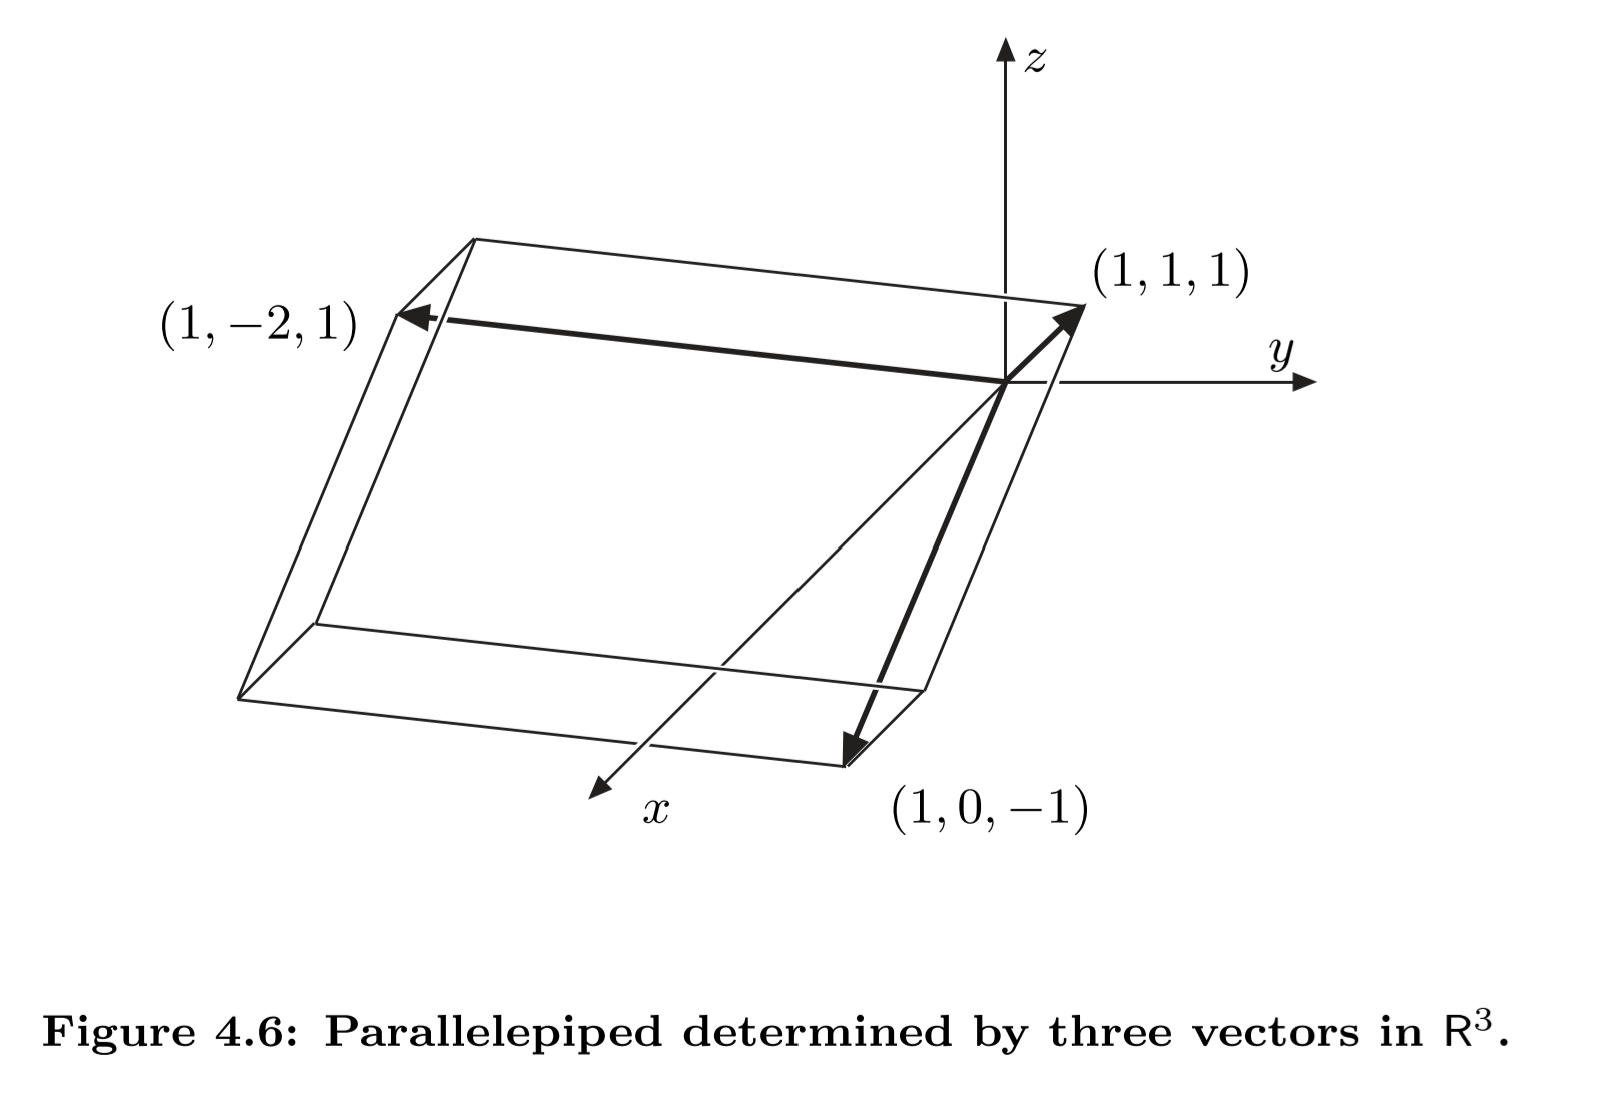
\includegraphics[width=16cm]{images/figure-4-6.png}

(BTW the figure doesn't look like a \emph{rectangular} parallelepiped.)

\begin{remark} \label{remark 4.3.4}
In our earlier discussion of the geometric significance of the determinant formed from the vectors in an ordered basis for \(\SET{R}^2\), we also saw that this determinant is positive if and only if the basis induces a \emph{right-handed coordinate system}.
(See \EXEC{4.1.13}.)
A similar statement is true in \(\SET{R}^n\).
\end{remark}

\begin{additional definition}
Specifically, if \(\gamma\) is any ordered basis for \(\SET{R}^{n}\)
and \(\beta\) is the \emph{standard} ordered basis for \(\SET{R}^n\), then \(\gamma\) induces a right-banded coordinate system if and only if \(\det(Q) > 0\), where \(Q\) is the \emph{change of coordinate matrix} that changes \(\gamma\)-coordinates into \(\beta\)-coordinates.
\end{additional definition}

Thus. for instance,
\[
    \gamma = \left\{
                \begin{pmatrix} 1 \\ 1 \\ 0 \end{pmatrix},
                \begin{pmatrix} 1 \\ -1 \\ 0 \end{pmatrix},
                \begin{pmatrix} 0 \\ 0 \\ 1 \end{pmatrix}
             \right\}
\]
induces a left-handed coordinate system in \(\SET{R}^3\) because the corresponding change of coordinate matrix (derived by \RMK{2.5.1} or \CORO{2.23.1})
\[
    \begin{pmatrix}
        1 & 1 & 0 \\
        1 & -1 & 0 \\
        0 & 0 & 1
    \end{pmatrix}
\]
has determinant \(-2 < 0\), whereas
\[
    \gamma' = \left\{
                \begin{pmatrix} 1 \\ 2 \\ 0 \end{pmatrix},
                \begin{pmatrix} -2 \\ 1 \\ 0 \end{pmatrix},
                \begin{pmatrix} 0 \\ 0 \\ 1 \end{pmatrix}
             \right\}
\]
induces a right-handed coordinate system in \(\SET{R}^3\) because the change of coordinate matrix (again derived by \RMK{2.5.1} or \CORO{2.23.1})
\[
    \begin{pmatrix}
        1 & -2 & 0 \\
        2 & 1 & 0 \\
        0 & 0 & 1
    \end{pmatrix}
\]
has determinant \(5 > 0\).

More generally, if \(\beta\) and \(\gamma\) are two ordered bases for \(\SET{R}^n\), then the coordinate systems induced by \(\beta\) and \(\alpha\) have the \emph{same orientation} (either both are right-handed or both are left-handed)
if and only if \(\det(Q) > 0\), where \(Q\) is the change of coordinate matrix that changes \(\gamma\)-coordinates into \(\beta\)-coordinates.

\exercisesection

\begin{exercise} \label{exercise 4.3.1}
Label the following statements as true or false.
\begin{enumerate}
\item If \(E\) is an elementary matrix, then \(\det(E) = \pm 1\).
\item For any \(A, B \in M_{n \X n}(F)\), \(\det(AB) = \det(A) \cdot \det(B)\).
\item A matrix \(M \in M_{n \X n}(F)\) is invertible if and only if \(\det(M) = 0\).
\item A matrix \(M \in M_{n \X n}(F)\) has rank \(n\) if and only if \(\det(M) \ne 0\).
\item For any \(A \in M_{n \X n}(F)\), \(\det(A^\top) = -\det(A)\).
\item The determinant of a square matrix can be evaluated by cofactor expansion along any \emph{column}.
\item Every system of \(n\) linear equations in \(n\) unknowns can be solved by Cramer's rule.
\item Let \(Ax = b\) be the matrix form of a system of \(n\) linear equations in \(n\) unknowns, where \(x = (x_1, x_2, ..., x_n)^\top\).
If \(\det(A) \ne 0\) and if \(M_k\) is the \(n \X n\) matrix obtained from \(A\) by replacing \RED{row} \(k\) of \(A\) by \(b^\top\), then the unique solution of \(Ax = b\) is
\[
    x_k = \cfrac{\det(M_k)}{\det(A)} \text{ for } k = 1, 2, ..., n.
\]
\end{enumerate}
\end{exercise}

\begin{proof} \ 

\begin{enumerate}
\item False. Type 2 with scalar \(c\) has determinant \(c\).
\item True by \THM{4.7}.
\item False by \CORO{4.7.1}.
\item True. \(M\) has rank \(n\), iff (by \RMK{3.2.1}) \(M\) is invertible, iff (by \CORO{4.7.1}) \(\det(M) \ne 0\).
\item False by \THM{4.8}.
\item True.
    We have \(\det(A) = \det(A^\top)\) by \THM{4.8}.
    And (by \THM{4.4}) \(\det(A^\top)\) is equal to the cofactor expansion along any \emph{row} of \(A^\top\).
    But that is equivalent to the cofactor expansion along any \(\emph{column}\) of \(A\).
\item False.
    The corresponding coefficient matrix also needs to be invertible.
\item False. By \THM{4.9}, \(M_k\) should be the \(n \X n\) matrix obtained from \(A\) by replacing \RED{column} \(k\) of \(A\) by \(b^\top\).
\end{enumerate}
\end{proof}

\begin{exercise} \label{exercise 4.3.2}
Solve the system using Cramer's rule:
\begin{align*}
    a_{11} x_1 + a_{12} x_2 & = b_1 \\
    a_{21} x_1 + a_{22} x_2 & = b_2
\end{align*}
where \(a_{11} a_{22} - a_{12} a_{21} \ne 0\).
\end{exercise}

\begin{proof}
By the given supposition, the corresponding coefficient matrix of the system
\[
    A = \begin{pmatrix} a_{11} & a_{12} \\ a_{21} & a_{22} \end{pmatrix}
\]
has nonzero determinant.
So using \THM{4.9} Cramer's rule,
\[
    M_1 = \begin{pmatrix} b_1 & a_{12} \\ b_2 & a_{22} \end{pmatrix}, \quad
    M_2 = \begin{pmatrix} a_{11} & b_1 \\ a_{21} & b_2 \end{pmatrix},
\]
and
\[
    x_1 = \cfrac{\det(M_1)}{\det(A)} = \cfrac{b_1 a_{22} - a_{12} b_2}{a_{11} a_{22} - a_{12} a_{21}},
    \quad
    x_2 = \cfrac{\det(M_2)}{\det(A)} = \cfrac{a_{11} b_2 - b_1 a_{21}}{a_{11} a_{22} - a_{12} a_{21}}
\]
\end{proof}

Exercise 3 to Exercise 7 are pure calculation problems that require solving systems using Cramer's rule. Skip.

\setcounter{exercise}{7}
\begin{exercise} \label{exercise 4.3.8}
Use \THM{4.8} to prove a result analogous to \THM{4.3}, but for columns.
\end{exercise}

\begin{proof}
Let \(A \in M_{n \X n}(F)\) such that
\[
    A = \begin{pmatrix} a_1 & a_2 & ... & a_r & ... & a_n
    \end{pmatrix},
\]
where \(a_1, ..., a_n \in F^n\) are columns of \(A\).
Now let \(a_r = u + kv\) for some \(u, v \in F^n\) and scalar \(k\), and let \(B, C\) be the same as \(A\) except for replacing row \(r\) with \(u\) and \(v\), respectively.

Then we need to show \(\det(A) = \det(B) + k \cdot \det(C)\).
Then
\begin{align*}
    \det(A) & = \det(A^\top) & \text{by \THM{4.8}} \\
            & = \det \begin{pmatrix} a_1^\top \\ \vdots \\ a_r^\top \\ \vdots \\ a_n^\top \end{pmatrix} = \det \begin{pmatrix} a_1^\top \\ \vdots \\ u^\top + k \cdot v^\top \\ \vdots \\ a_n^\top \end{pmatrix} & \text{of course} \\
            & = \det \begin{pmatrix} a_1^\top \\ \vdots \\ u^\top \\ \vdots \\ a_n^\top \end{pmatrix} + k \cdot \det \begin{pmatrix} a_1^\top \\ \vdots \\ v^\top \\ \vdots \\ a_n^\top \end{pmatrix} & \text{by \THM{4.3}} \\
            & = \det(B^\top) + k \cdot \det(C^\top) & \text{of course} \\
            & = \det(B) + k \cdot \det(C), & \text{by \THM{4.8}}
\end{align*}
as desired.
\end{proof}

\begin{exercise} \label{exercise 4.3.9}
Prove that an \emph{upper triangular} \(n \X n\) matrix is invertible if and only if all its diagonal entries are nonzero.
\end{exercise}

\begin{proof}
An \emph{upper triangular} \(n \X n\) matrix is invertible, iff (by \CORO{4.7.1}) its determinant is nonzero, iff (by \EXEC{4.2.23}) the product of its diagonal entries are nonzero, iff (of course) all its diagonal entries are nonzero.
\end{proof}

\begin{exercise} \label{exercise 4.3.10}
A matrix \(M \in M_{n \X n}(F)\) is called \href{https://www.wikiwand.com/en/Nilpotent_matrix}{nilpotent} if, for some \emph{positive} integer \(k\), \(M^k = O\), where \(O\) is the \(n \X n\) zero matrix.
Prove that if \(M\) is nilpotent, then \(\det(M) = 0\).
\end{exercise}

\begin{note}
Concept-related exercise: \EXEC{2.3.16}(b).
\end{note}

\begin{proof}
We have
\begin{align*}
             & M^k = O \\
    \implies & \det(M^k) = \det(O) = 0 & \text{of course} \\
    \implies & \det(M)^k = 0 & \text{by \THM{4.7}} \\
    \implies & \det(M) = 0 & \text{of course}
\end{align*}
\end{proof}

\begin{exercise} \label{exercise 4.3.11}
A matrix \(M \in M_{n \X n}(\SET{C})\) is called \textbf{skew-symmetric} if \(M^\top = -M\).
Prove that if \(M\) is skew-symmetric and \(n\) is odd, then \(M\) is not invertible.
What happens if \(n\) is even?
\end{exercise}

\begin{note}
The complex number has characteristic \(0 \ne 2\).
The exercise would not apply if the field of the matrix has characteristic equal to \(2\).
\end{note}

\begin{proof}
By \EXEC{4.2.25}, we have \(\det(-M) = (-1)^n \det(M)\).
And by \THM{4.8}, we have \(\det(M^\top) = \det(M)\).
And by supposition \(-M = M^\top\), so we have \((-1)^n \det(M) = \det(M)\).
If \(n\) is odd, the equation implies \(-1 \det(M) = \det(M)\).
Which implies \(\det(M) = 0 \in \SET{C}\).
If \(n\) is even, then that only implies \(\det(M) = \det(M)\), hence we cannot conclude anything.
For example, (the skew-symmetric matrix) \(\begin{pmatrix} 0 & 1 \\ -1 & 0 \end{pmatrix}\) is invertible, but (the skew-symmetric matrix) \(O_{2 \X 2}\) is not invertible.
\end{proof}

\begin{exercise} \label{exercise 4.3.12}
A matrix \(Q \in M_{n \X n}(\SET{R})\) is called \textbf{orthogonal} if \(QQ^\top = I\).
Prove that if \(Q\) is orthogonal, then \(\det(Q) = \pm 1\).
\end{exercise}

\begin{note}
This exercise should be related to \CH{6}.
\end{note}

\begin{proof}
We have
\begin{align*}
    1 = \det(I) & = \det(QQ^\top) & \text{by supposition} \\
                & = \det(Q) \det(Q^\top) & \text{by \THM{4.7}} \\
                & = \det(Q) \det(Q), & \text{by \THM{4.8}} \\
\end{align*}
which implies \(\det(Q) = \pm 1\).
\end{proof}

\begin{exercise} \label{exercise 4.3.13}
For \(M \in M_{n \X n}(\SET{C})\), let \(\conjugatet{M}\) be the matrix such that \((\conjugatet{M})_{ij} = \conjugatet{M_{ij}}\) for all \(i, j\),
where \(\conjugatet{M_{ij}}\) is the complex conjugate of \(M_{ij}\).
\begin{enumerate}
\item Prove that \(\det(\conjugatet{M}) = \conjugatet{\det(M)}\).

\item A matrix \(Q \in M_{n \X n}(\SET{C})\) is called \textbf{unitary} if \(QQ^* = I\), where \(Q^* = \conjugatet{Q^\top}\).
Prove that if \(Q\) is a \emph{unitary} matrix, then \(\left| \det(Q) \right| = 1\).
\end{enumerate}
\end{exercise}

\begin{proof} \ 

\begin{enumerate}
\item We prove by induction on \(n\).
For \(n = 1\),
\begin{align*}
    \det(\conjugatet{M}) & = (\conjugatet{M})_{11} & \text{by \DEF{4.2} for dimension \(= 1\)} \\
                         & = \conjugatet{M_{11}} & \text{by supposition} \\
                         & = \conjugatet{\det(M)} & \text{by \DEF{4.2} for dimension \(= 1\)}
\end{align*}

Suppose inductively \(\det(\conjugatet{M}) = \conjugatet{\det(M)}\) for arbitrary \(M \in M_{k \X k}(\SET{C})\) such that \((\conjugatet{M})_{ij} = \conjugatet{M_{ij}}\) for all \(i, j\).
We have to show \(\det(\conjugatet{M}) = \conjugatet{\det(M)}\) for arbitrary \(M \in M_{(k + 1) \X (k + 1)}(\SET{C})\) such that \((\conjugatet{M})_{ij} = \conjugatet{M_{ij}}\) for all \(i, j\).
Then
\begin{align*}
    \det(\conjugatet{M}) & = \sum_{j = 1}^{(k + 1)} (\conjugatet{M})_{1j} \cdot (-1)^{1 + j} \cdot \det(\widetilde{(\conjugatet{M})}_{1j}) & \text{by \DEF{4.2}} \\
                         & = \sum_{j = 1}^{(k + 1)} \RED{\conjugatet{M_{1j}}} \cdot (-1)^{1 + j} \cdot \det(\widetilde{(\conjugatet{M})}_{1j}) & \text{by supposition} \\
                         & = \sum_{j = 1}^{(k + 1)} \conjugatet{M_{1j}} \cdot (-1)^{1 + j} \cdot \RED{\conjugatet{\det(\tilde{M}_{1j})}} & \text{by inductive hypothesis} \\
                         & = \sum_{j = 1}^{(k + 1)} \conjugatet{M_{1j} \cdot (-1)^{1 + j}} \cdot \conjugatet{\det(\tilde{M}_{1j})} & \text{of course (see theorem D.2(c)(e))} \\
                         & = \sum_{j = 1}^{(k + 1)} \conjugatet{M_{1j} \cdot (-1)^{1 + j} \cdot \det(\tilde{M}_{1j})} & \text{of course (see theorem D.2)(c)} \\
                         \\
                         & = \conjugatet{\sum_{j = 1}^{(k + 1)} M_{1j} \cdot (-1)^{1 + j} \cdot \det(\tilde{M}_{1j})} & \text{of course (see theorem D.2)(b)} \\
                         & = \conjugatet{\det(M)} & \text{by \DEF{4.2}}
\end{align*}

\item We have
\begin{align*}
    1 = \det(I) & = \det(QQ^*) & \text{by supposition} \\
                & = \det(Q) \det(Q^*) & \text{by \THM{4.7}} \\
                & = \det(Q) \det(\conjugatet{Q^\top}) & \text{by definition} \\
                & = \det(Q) \conjugatet{\det(Q^\top)} & \text{by part(a)} \\
                & = \det(Q) \conjugatet{\det(Q)} & \text{by \THM{4.8}} \\
                & = \abs{\det(Q)}^2, & \text{by definition in page 551}
\end{align*}
which implies \(\abs{\det(Q)} = 1\).
\end{enumerate}
\end{proof}

\begin{exercise} \label{exercise 4.3.14}
Let \(\beta = \{ u_1, u_2, ..., u_n \}\) be a subset of \(F^n\) containing \(n\) distinct vectors, and let \(B\) be the matrix in \(M_{n \X n}(F)\) having \(u_j\) as column \(j\).
Prove that \(\beta\) is a basis for \(F^n\) if and only if \(\det(B) \ne 0\).
\end{exercise}

\begin{proof}
We have \(\beta\) is a basis for \(F^n\) iff (by \CH{3}) \(\rank(B) = n\), iff (by \EXEC{4.3.1}(d)) \(\det(B) \ne 0\).
\end{proof}

\begin{exercise} \label{exercise 4.3.15}
Prove that if \(A, B \in M_{n \X n}(F)\) are \emph{similar}, then \(\det(A) = \det(B)\).
\end{exercise}

\begin{proof}
If \(A, B \in M_{n \X n}(F)\) are similar, then by \DEF{2.16} we have \(B = Q^{-1} A Q\) for some invertible \(Q\).
And
\begin{align*}
    \det(B) & = \det(Q^{-1} A Q) \\
            & = \det(Q^{-1}) \det(A) \det(Q) & \text{by \THM{4.7}} \\
            & = \det(Q^{-1}) \det(Q) \det(A) & \text{of course} \\
            & = \det(Q^{-1} Q) \det(A) & \text{by \THM{4.7}} \\
            & = \det(I) \det(A) & \text{of course} \\
            & = 1 \cdot \det(A) = \det(A) & \text{of course}
\end{align*}
\end{proof}

\begin{exercise} \label{exercise 4.3.16}
Use determinants to prove that if \(A, B \in M_{n \X n}(F)\) are such that \(AB = I\), then \(A\) is invertible (and hence \(B = A^{-1}\)).
\end{exercise}

\begin{note}
This is related to \ATHM{2.38}.
\end{note}

\begin{proof}
We have
\begin{align*}
    1 = \det(I) & = \det(AB) & \text{by supposition} \\
                & = \det(A) \det(B), & \text{by \THM{4.7}}
\end{align*}
which implies both \(\det(A)\) and \(\det(B)\) cannot be zero.
And in particular by \CORO{4.7.1}, \(A\) is invertible.
And by \ATHM{2.38}(1), \(B = A^{-1}\).
\end{proof}

\begin{exercise} \label{exercise 4.3.17}
Let \(A, B \in M_{n \X n}(F)\) be such that \(AB = -BA\).
Prove that if \(n\) is odd and \(F\) is \emph{not} a field of characteristic two, then \(A\) or \(B\) is not invertible.
\end{exercise}

\begin{proof}
We have
\begin{align*}
    \det(A) \det(B) & = \det(AB) & \text{by \THM{4.7}} \\
                    & = \det(-BA) & \text{by supposition} \\
                    & = (-1)^n \cdot \det(BA) & \text{by \EXEC{4.2.25}} \\
                    & = (-1) \cdot \det(BA) & \text{since \(n\) is odd} \\
                    & = -1 \cdot \det(B) \det(A) & \text{by \THM{4.7}} \\
                    & = -1 \cdot \det(A) \det(B) & \text{of course} \\
    \implies 2 \cdot \det(A) \det(B) = 0.
\end{align*}
Since \(F\) is \emph{not} a field of characteristic two, that implies \(\det(A) \det(B) = 0\), so \(\det(A)\) \emph{or} \(\det(B)\) is zero, so by \CORO{4.7.1}, \(A\) or \(B\) is not invertible.
\end{proof}

\begin{exercise} \label{exercise 4.3.18}
Complete the proof of \THM{4.7} by showing that if \(A\) is an \emph{elementary matrix} of type 2 or type 3, then \(\det(AB) = \det(A) \cdot \det(B)\).
\end{exercise}

\begin{proof}
If \(A\) is type 2, then \(A\) has the form
\[
    A = \begin{pmatrix}
        e_1 \\ e_2 \\ \vdots \\ k e_i \\ \vdots \\ e_n
    \end{pmatrix}
\]
where \(k\) is nonzero scalar.
And by \THM{3.1}, \(AB\) is equal to \(B\) with row \(i\) multiplied by \(k\), so by \RMK{4.2.3}(b), \(\det(AB) = k \cdot \det(B)\) \MAROON{(1)}.
And by \RMK{4.3.1}, \(\det(A) = k\), hence by \MAROON{(1)} we have \(\det(AB) = \det(A) \cdot \det(B)\).

If \(A\) is type 3, then \(A\) has the form
\[
    A = \begin{pmatrix}
        e_1 \\ e_2 \\ \vdots \\ k e_i + e_j \\ \vdots \\ e_n
    \end{pmatrix}
\]
And by \THM{3.1}, \(AB\) is equal to \(B\) but adding \(k\) times row \(i\) to row \(j\), so by \RMK{4.2.3}(c), \(\det(AB) = \det(B)\) \MAROON{(2)}.
And by \RMK{4.3.1}, \(\det(A) = 1\), hence by \MAROON{(2)} we have \(\det(AB) = \det(B) = 1 \cdot \det(B) = \det(A) \cdot \det(B)\).
\end{proof}

\begin{exercise} \label{exercise 4.3.19}
A matrix \(A \in M_{n \X n}(F)\) is called \textbf{lower triangular} if \(A_{ij} = 0\) for \(1 \le i < j \le n\).
Suppose that \(A\) is a lower triangular matrix.
Describe \(\det(A)\) in terms of the entries of \(A\).
\end{exercise}

\begin{proof}
If \(A\) is lower triangular, then \(A^\top\) is upper triangular.
By \THM{4.8}, \(\det(A) = \det(A^\top)\).
And by \EXEC{4.2.23}, we know \(\det(A^\top)\) is equal to the product of its diagonals, so \(\det(A)\) is equal to the product of \(A^\top\)'s diagonals.
But \(A^\top\)'s diagonals are of course \(A\)'s diagonals, so \(\det(A)\) is also equal to the product of its diagonals.
\end{proof}

\begin{exercise} \label{exercise 4.3.20}
Suppose that \(M \in M_{n \X n}(F)\) can be written in the form
\[
    M = \begin{pmatrix} A & B \\ O & I \end{pmatrix},
\]
where \(A\) is a \emph{square} matrix.
Prove that \(\det(M) = \det(A)\).
\end{exercise}

\begin{proof}
Informally, if we expand the last row of \(M\), then ultimately we have
\[
    \det(M) = 1 \cdot 1 \cdot ... \cdot 1 \cdot \det(A) = \det(A).
\]
\end{proof}

\begin{exercise} \label{exercise 4.3.21}
Prove that if \(M \in M_{n \X n}(F)\) can be written in the form
\[
    M = \begin{pmatrix} A & B \\ O & C \end{pmatrix},
\]
where \(A\) and \(C\) are square matrices, then \(\det(M) = \det(A) \cdot \det(C)\).
\end{exercise}

\begin{proof}
There are two cases: \(C\) is invertible or not.

If \(C\) is not invertible, then the rows of \(C\) is \emph{not} \LID{}, and (by \CORO{4.7.1}) \(\det(C) = 0\);
and of course the rows of \((O|C)\) is not \LID{}, which implies \(M\) has rank less then \(n\), so (by \CORO{4.6.1}) \(\det(M) = 0\).
And \(\det(A) \cdot \det(C) = \det(A) \cdot 0 = 0\), hence \(\det(M) = \det(A) \cdot \det(C)\).

If \(C\) is invertible, then given the matrix
\[
    M' = \begin{pmatrix} I & O \\ O & C^{-1} \end{pmatrix},
    M'' = \begin{pmatrix} A & B \\ O & I \end{pmatrix},
\]
by (the generalization of) \ATHM{3.7},
\[
    M' M =
    \begin{pmatrix} I & O \\ O & C^{-1} \end{pmatrix}
    \begin{pmatrix} A & B \\ O & C \end{pmatrix}
    = M'',
\]
So we have \(\det(M' M) = \det(M'')\), so by \THM{4.7}, \(\det(M')\det(M) = \det(M'')\) \MAROON{(1)}.
By (similar argument of) \EXEC{4.3.20}, \(\det(M') = \det(C^{-1})\).
And by \EXEC{4.3.20}, \(\det(M'') = \det(A)\), so by \MAROON{(1)}, we have \(\det(C^{-1}) \det(M) = \det(A)\).
And by \CORO{4.7.1}, that implies
\[
    \cfrac{1}{\det(C)} \det(M) = \det(A), \text{ so } \det(M) = \det(A) \cdot \det(C).
\]
So in all cases, we have \(\det(M) = \det(A) \cdot \det(C)\).
\end{proof}

\begin{exercise} \label{exercise 4.3.22}
Let \(\T : \POLYNF \to F^{n + 1}\) be the \LTRAN{} defined in \EXEC{2.4.22} by \(\T(f) = (f(c_0), f(c_1), ..., f(c_n))\), where \(c_0, c_1, ..., c_n\) are \emph{distinct} scalars in an infinite field \(F\).
Let \(\beta\) be the \emph{standard} ordered basis for \(\POLYNF\) and \(\gamma\) be the \emph{standard} ordered basis for \(F^{n + 1}\).
\begin{enumerate}
\item Show that the \((n + 1) \X (n + 1)\) matrix \(M = [\T]_{\beta}^{\gamma}\) has the form
\[
    \begin{pmatrix}
        1 & c_0 & c_0^2 & ... & c_0^n \\\
        \vdots & \vdots & \vdots & & \vdots \\
        1 & c_{n-1} & c_{n-1}^2 & ... & c_{n-1}^n \\
        1 & c_n & c_n^2 & ... & c_n^n
    \end{pmatrix}
\]
A matrix with this form is called a \textbf{Vandermonde matrix}.
\item Use \EXEC{2.4.22} to prove that \(\det(M) \ne 0\).
\item Prove that
\[
    \det(M) = \prod_{0 \le i < j \le n} (c_j - c_i),
\]
the product of all terms of the form \(c_j - c_i\) for \(0 \le i < j \le n\).
\end{enumerate}
\end{exercise}

\begin{proof} \ 

\begin{enumerate}
\item
For the standard ordered base \(\beta = \{ 1, x, x^2, ..., x^n \}\), we have
\begin{align*}
    \T(1) & = (1, 1, ..., 1) = 1 \cdot e_1 + 1 \cdot e_2 + ... + 1 \cdot e_{n+1} \\
    \T(x) & = (c_0, c_1, ..., c_n) = c_0 \cdot e_1 + c_1 \cdot e_2 + ... + c_n \cdot e_{n+1} \\
    \T(x^2) & = (c_0^2, c_1^2, ..., c_n^2) = c_0^2 \cdot e_1 + c_1^2 \cdot e_2 + ... + c_n^2 \cdot e_{n+1} \\
    \vdots \\
    \T(x^n) & = (c_0^n, c_1^n, ..., c_n^n) = c_0^n \cdot e_1 + c_1^n \cdot e_2 + ... + c_n^n \cdot e_{n+1}
\end{align*}
So \([\T]_{\beta}^{\gamma}\) has that desired form.

\item \(\T\) is an isomorphism, so by \THM{2.18}, \(M = [\T]_{\beta}^{\gamma}\) is invertible, so by \CORO{4.7.1}, \(\det(M) \ne 0\).

\item Let
\[
    F_1 = \begin{pmatrix}
        1 & c_0 & c_0^2 & ... & c_0^n \\\
        \vdots & \vdots & \vdots & & \vdots \\
        1 & c_{n-1} & c_{n-1}^2 & ... & c_{n-1}^n \\
        1 & x & x^2 & ... & x^n
    \end{pmatrix}
    \quad \text{and } \quad
    f_1(x) = \det (F_1).
\]
Then its clear that, by expanding the last row of \(F_1\), \(f_1(x)\) is a polynomial of degree \(n\).
And in particular,
\[
    f_1(c_n) = \det(M) \quad \quad \MAROON{(1.1)}.
\]
Furthermore, \(c_0, c_1, ..., c_{n-1}\) are the \(n\) roots of this polynomial, since from the structure of \(F_1\), if we replace \(x\) with \(c_0, ..., c_{n - 1}\), then \(F_1\) has two identical rows, so (by \CORO{4.4.1}) the determinant is equal to zero.
So \(f_1(x)\) has the form
\[
    f_1(x) = \alpha_1 (x - c_0)(x - c_1) ... (x - c_{n - 1}), \quad \quad \MAROON{(1.2)}
\]
where \(\alpha_1\) is a nonzero scalar.
\textbf{But again}, from the structure of \(F_1\), \(\alpha_1\) is in fact equal to the cofactor of the row \(n + 1\), column \(n + 1\).
That is,
\[
    \alpha_1 = (-1)^{(n + 1) + (n + 1)} \det \left( \widetilde{F_1}_{(n+1)(n+1)} \right) = \det\left( \widetilde{F_1}_{(n+1)(n+1)} \right).
\]
\emph{That is},
\[
    \alpha_1 = \det \begin{pmatrix}
        1 & c_0 & c_0^2 & ... & c_0^{n \RED{- 1}} \\\
        \vdots & \vdots & \vdots & & \vdots \\
        1 & c_{n \RED{-1}} & c_{n \RED{-1}}^2 & ... & c_{n \RED{-1}}^{n \RED{- 1}}
    \end{pmatrix}. \quad \quad \MAROON{(1.3)}
\]
Now if we \textbf{use the same argument again}, then we let
\[
    F_2 = \begin{pmatrix}
        1 & c_0 & c_0^2 & ... & c_0^{n - 1} \\\
        \vdots & \vdots & \vdots & & \vdots \\
        1 & c_{n-2} & c_{n-2}^2 & ... & c_{n-2}^{n - 1} \\
        1 & x & x^2 & ... & x^{n-1}
    \end{pmatrix}
    \quad \text{and} \quad
    f_2(x) = \det(F_2).
\]
Then in particular, by observation,
\[
    f_2(c_{n - 1}) = \alpha_1 \quad \quad \MAROON{(2.1)}.
\]
Using the same argument, we have
\[
    f_2(x) = \alpha_2 (x - c_0)(x - c_1) ... (x - c_{n - 2}), \quad \quad \MAROON{(2.2)}
\]
where
\[
    \alpha_2 = \det \begin{pmatrix}
        1 & c_0 & c_0^2 & ... & c_0^{n \RED{- 2}} \\\
        \vdots & \vdots & \vdots & & \vdots \\
        1 & c_{n \RED{-2}} & c_{n \RED{-2}}^2 & ... & c_{n \RED{-2}}^{n \RED{- 2}}
    \end{pmatrix}. \quad \quad \MAROON{(2.3)}
\]

Continue this process \emph{inductively}, we have
\begin{align*}
    \det(M) & = f_1(c_n) & \text{by \MAROON{(1.1)}} \\
            & = \alpha_1 \cdot (c_n - c_0) (c_n - c_1) ... (c_n - c_{n - 1}) & \text{by \MAROON{(1.2)}} \\
            & = f_2(c_{n - 1}) \cdot [(c_n - c_0) (c_n - c_1) ... (c_n - c_{n - 1})] & \text{by \MAROON{(2.1)}} \\
            & = \big[ \alpha_2 (c_{n - 1} - c_0) (c_{n - 1} - c_1) ... (c_{n - 1} - c_{n - 2}) \big] \\
            & \quad \quad \cdot \big[ (c_n - c_0) (c_n - c_1) ... (c_n - c_{n - 1}) \big] & \text{by \MAROON{(2.2)}} \\
            & \quad \vdots \\
            & = \big[(c_1 - c_0)] \big[(c_2 - c_0) (c_2 - c_1) ] \\
            & \quad \quad \cdot ... \\
            & \quad \quad \cdot \big[ (c_{n - 1} - c_0) (c_{n - 1} - c_1) ... (c_{n - 1} - c_{n - 2}) \big] \\
            & \quad \quad \cdot \big[ (c_n - c_0) (c_n - c_1) ... (c_n - c_{n - 1}) \big] & \text{expand inductively} \\
            & = \prod_{0 \le i < j \le n} (c_j - c_i).
\end{align*}
\end{enumerate}
\end{proof}

\begin{exercise} \label{exercise 4.3.23}
Let \(A \in M_{n \X n}(F)\) be nonzero.
For any \(m\) (\(1 \le m \le n\)), an \(m \X m\) \textbf{submatrix} is obtained by deleting \emph{any} \(n - m\) rows and any \(n - m\) columns of \(A\).
(The concept is similar to a \emph{subsequence} of a sequence.)
\begin{enumerate}
\item Let \(k\) (\(1 \le k \le n\)) denote the \emph{largest} integer such that some \(k \X k\) submatrix has a nonzero determinant.
Prove that \(\rank(A) = k\).
\item Conversely, suppose that \(\rank(A) = k\).
Prove that there exists a \(k \X k\) submatrix with a nonzero determinant.
\end{enumerate}
\end{exercise}

\begin{proof} \ 

\begin{enumerate}
\item
If \(\rank(A) = n\), that means \(A\) is invertible, and by \CORO{4.7.1}, \(\det(A) \ne 0\).
So the largest submatrix with a nonzero determinant is \(A\) itself, which has size \(n \X n\), so in this case, \(k = n\), which is equal to \(\rank(A)\).

Now suppose \(\rank(A) < n\).
We will show that \(\rank(A) < k\) and \(\rank(A) > k\) lead to contradiction.

So for the sake of contradiction, suppose
\[
    \rank(A) < k. \quad \quad \BLUE{(1)}
\]
First let \(B\) be the \(k \X k\) submatrix of \(A\) with nonzero determinant.
Then by \CORO{4.7.1}, \(B\) is invertible, and the columns \(S = \{ v_1, v_2, ..., v_k \}\) of \(B\) are \LID{}.
Now consider the \(k \X \RED{n}\) submatrix \(C\) of \(A\) obtained by deleting those rows who were deleted when we construct \(B\).
Then \(S\) is a \emph{subset} of the columns of \(C\).
This means \(\rank(C) \ge \#S = k\).
But by \THM{3.6}, \(\rank(C) \le \min(k, n) = k\).
Hence \(\rank(C) = k\), which implies the \(k\) rows of \(C\) are also \LID{}.
And thus the matrix \(A\) contains these \(k\) \LID{} rows and hence \(\rank(A) \ge k\), which contradicts \BLUE{(1)}.

Now, for the sake of contradiction, suppose
\[
    \rank(A) > k. \quad \quad \BLUE{(2)}
\]
Let \(\rank(A) = r\).
Then we can pick \(r\) \LID{} rows of \(A\), say \(u_1, ..., u_r\), to construct a \(r \X n\) submatrix \(D\) of \(A\).
Then \(D\) has \(\rank(D) \ge r\).
And by \THM{3.6}, \(\rank(D) \le \min(r, n) = r\), hence \(\rank(D) = r\).
Now we can also pick \(r\) \LID{} \emph{columns}, say \(v_1, ..., v_r\), of \(D\), to construct an \(r \X r\) submatrix \(D'\) of \(D\).
Note that \(D'\) is also a submatrix of \(A\).
Then \(\rank(D') \ge r\), and again by \THM{3.6}, \(\rank(D') \le min(r, r) = r\), hence \(\rank(D') = r\).
This implies \(D'\) is invertible, and by \CORO{4.7.1}, \(\det(D') \ne 0\).
So we have found a \(r \X r\) submatrix of \(A\) with nonzero determinant and \(r > k\), which contradicts the property of \(k\) that \(k\) is the size of the ``largest'' nonzero determinant submatrix of \(A\).

So \(\rank(A)\) must be equal to \(k\).

\item This is similar to the second part of the proof in part(a),
We just pick \(k\) \LID{} rows of \(A\) to construct a \(k \X n\) submatrix, and pick \LID{} \(k\) columns of that submatrix to construct a \(k \X k\) submatrix.
Then such \(k \X k\) matrix is a submatrix of \(A\) and has nonzero determinant.
\end{enumerate}
\end{proof}

\begin{exercise} \label{exercise 4.3.24}
Let \(A \in M_{n \X n}(F)\) have the form
\[
    A = \left(\begin{array}{rrcccc}
        0 & 0 & 0 & \cdots & 0 & a_{0} \\
        -1 & 0 & 0 & \cdots & 0 & a_{1} \\
        0 & -1 & 0 & \cdots & 0 & a_{2} \\
        \vdots & \vdots & \vdots & \ddots & \vdots & \vdots \\
        0 & 0 & 0 & \cdots & 0 & a_{n-2} \\
        0 & 0 & 0 & \cdots & -1 & a_{n-1}
    \end{array}\right)
\]
Compute \(\det(A + tI)\), where \(I\) is the \(n \X n\) identity matrix.
\end{exercise}

\begin{proof}
\(A + tI\) has the form
\[
    \begin{pmatrix}
        t      & 0      & 0      & \cdots & 0      & a_{0} \\
        -1     & t      & 0      & \cdots & 0      & a_{1} \\
        0      & -1     & t      & \cdots & 0      & a_{2} \\
        \vdots & \vdots & \vdots & \ddots & \vdots & \vdots \\
        0      & 0      & 0      & \cdots & t      & a_{n-2} \\
        0      & 0      & 0      & \cdots & -1     & t + a_{n-1}
    \end{pmatrix}
\]
We perform type 3 elementary row operations:
\begin{align*}
    \begin{pmatrix}
        t      & 0      & 0      & \cdots & 0      & a_{0} \\
        -1     & t      & 0      & \cdots & 0      & a_{1} \\
        0      & -1     & t      & \cdots & 0      & a_{2} \\
        \vdots & \vdots & \vdots & \ddots & \vdots & \vdots \\
        0      & 0      & 0      & \cdots & t      & a_{n-2} \\
        0      & 0      & 0      & \cdots & -1     & t + a_{n-1}  
    \end{pmatrix}
    \to
    \begin{pmatrix}
        t       & 0      & 0      & \cdots & 0      & a_{0} \\
        \RED{0} & t      & 0      & \cdots & 0      & \RED{a_{1} + \cfrac{a_0}{t}} \\
        0       & -1     & t      & \cdots & 0      & a_{2} \\
        \vdots  & \vdots & \vdots & \ddots & \vdots & \vdots \\
        0      & 0      & 0      & \cdots & t      & a_{n-2} \\
        0       & 0      & 0      & \cdots & -1     & t + a_{n-1}  
    \end{pmatrix} \\
    \to
    \begin{pmatrix}
        t       & 0       & 0      & \cdots & 0      & a_{0} \\
        0       & t       & 0      & \cdots & 0      & a_{1} + \cfrac{a_0}{t} \\
        0       & \RED{0} & t      & \cdots & 0      & \RED{a_{2} + \cfrac{a_{1}}{t} + \cfrac{a_0}{t^2}} \\
        \vdots  & \vdots  & \vdots & \ddots & \vdots & \vdots \\
        0       & 0       & 0      & \cdots & t      & a_{n-2} \\
        0       & 0       & 0      & \cdots & -1     & t + a_{n-1}   
    \end{pmatrix}
    \to ... \to
    \begin{pmatrix}
        t       & 0       & 0      & \cdots & 0       & a_{0} \\
        0       & t       & 0      & \cdots & 0       & a_{1} + \cfrac{a_0}{t} \\
        0       & 0       & t      & \cdots & 0       & a_{2} + \cfrac{a_{1}}{t} + \cfrac{a_0}{t^2} \\
        \vdots  & \vdots  & \vdots & \ddots & \vdots  & \vdots \\
        0       & 0       & 0      & \cdots & t       & \vdots \\
        0       & 0       & 0      & \cdots & \RED{0} & \RED{t + a_{n-1} + \cfrac{a_{n-2}}{t} + ... + \cfrac{a_0}{t^{n-1}}}
    \end{pmatrix}
\end{align*}
which is upper triangular.
So by \EXEC{4.2.23}, the determinant is equal to the product of the diagonal entries, that is
\[
    t^{n - 1} (t + a_{n-1} + \cfrac{a_{n-2}}{t} + ... + \cfrac{a_0}{t^{n-1}})
    = t^n + t^{n - 1} a_{n - 1} + t^{n - 2} a_{n - 2} + ... + t a_1 + a_0.
\]
So \(\det(A) = t^n + t^{n - 1} a_{n - 1} + t^{n - 2} a_{n - 2} + ... + t a_1 + a_0\).
\end{proof}

\begin{exercise} \label{exercise 4.3.25}
Let \(c_{jk}\) denote the cofactor (see \DEF{4.2}) of the row \(j\), column \(k\) entry of the matrix \(A \in M_{n \X n}(F)\).
\begin{enumerate}
\item Prove that if \(B\) is the matrix obtained from \(A\) by replacing \emph{column} \(k\) by \(e_j\), then \(\det(B) = c_{jk}\).

\item Show that for \(1 \le j \le n\), we have
\[
    A \begin{pmatrix} c_{j1} \\ c_{j2} \\ \vdots \\ c_{jn} \end{pmatrix}
    = \det(A) \cdot e_j.
\]
Hint: Apply Cramer's rule to \(Ax = e_j\).

\item Deduce that if \(C\) is the \(n \X n\) matrix such that \(C_{ij} = c_{\RED{ji}}\), then \(AC = [\det(A)]I\).
(Notice the order of the suffix.)

\item Show that if \(\det(A) \ne 0\), then \(A^{-1} = [\det(A)]^{-1}C\).
\end{enumerate}
\end{exercise}

\begin{proof} \ 

\begin{enumerate}
\item Just expanding the column \(k\) of \(B\):
\begin{align*}
    \det(B) & = \sum_{i = 1}^n B_{ik} \cdot (-1)^{i + k} \det(\tilde{B}_{ik}) \\
            & = \sum_{i = 1}^n A_{ik} \cdot (-1)^{i + k} \det(\tilde{B}_{ik}) & \text{since \(A, B\) only differ in column \(k\)} \\
            & = \sum_{i = 1}^n B_{ik} \cdot c_{ik} & \text{by def of cofactor} \\
            & = 0 \cdot c_{1k} + ... + 1 \cdot c_{jk} + ... + 0 \cdot c_{nk} & \text{since column \(k\) of \(B = e_j\)} \\
            & = c_{jk}.
\end{align*}

\item We just check each entry of the product.
The product is
\begin{equation} \label{exec.4.3.25.eq}
    A \begin{pmatrix} c_{j1} \\ c_{j2} \\ \vdots \\ c_{jn} \end{pmatrix}
    = \begin{pmatrix}
        A_{11} c_{j1} + ... + A_{1n} c_{jn} \\
        A_{21} c_{j1} + ... + A_{2n} c_{jn} \\
        \vdots \\
        \RED{A_{j1} c_{j1} + ... + A_{jn} c_{jn}} \\
        \vdots \\
        A_{n1} c_{j1} + ... + A_{nn} c_{jn}
    \end{pmatrix}
    = \begin{pmatrix}
        \sum_{k = 1}^n A_{1k} c_{jk} \\
        \sum_{k = 1}^n A_{2k} c_{jk} \\
        \vdots \\
        \RED{\det(A)} \\
        \vdots \\
        \sum_{k = 1}^n A_{nk} c_{jk}
    \end{pmatrix}
\end{equation}
For the \(i\)th entry of the product where \(i \ne j\), it can be seen as the cofactor expansion of \(B_i\) that is obtained by replacing the \(j\)th row of \(A\) with the \(i\)th row of \(A\);
that is,
\[
    B_i = \begin{blockarray}{cccc}
        \begin{block}{(ccc)c}
        A_{11} & ... & A_{1n} & \\
        \vdots &     & \vdots & \\
        A_{i1} & ... & A_{in} & \RED{i} \\
        \vdots &     & \vdots & \\
        \RED{A_{i1}} & \RED{...} & \RED{A_{in}} & \RED{j}\\
        \vdots &     & \vdots & \\
        A_{n1} & ... & A_{nn} & \\
        \end{block}
    \end{blockarray}
\]
Since \(B_i\) has two identical rows, by \CORO{4.4.1}, \(\det(B_i) = 0\);
that is, the \(i\)th entry, where \(i \ne j\), of the product in \ref{exec.4.3.25.eq} is zero.
Hence
\[
    A \begin{pmatrix} c_{j1} \\ c_{j2} \\ \vdots \\ c_{jn} \end{pmatrix} = \begin{pmatrix}
        0 \\ \vdots \\ \det(A) \\ \vdots \\ 0
    \end{pmatrix} = \det(A) \cdot e_j.
\]

\item By the previous exercise
\begin{align*}
    AC & = A \begin{pmatrix}
            c_{11} & c_{21} & ... & c_{n1} \\
            c_{12} & c_{22} & ... & c_{n2} \\
            \vdots & \vdots &     & \vdots \\
            c_{1n} & c_{2n} & ... & c_{nn}
           \end{pmatrix} \\
       & = \begin{pmatrix}
           A \begin{pmatrix} c_{11} \\ c_{12} \\ \vdots \\ c_{1n} \end{pmatrix}
           & A \begin{pmatrix} c_{21} \\ c_{22} \\ \vdots \\ c_{2n} \end{pmatrix}
           & ...
           & A \begin{pmatrix} c_{n1} \\ c_{n2} \\ \vdots \\ c_{nn} \end{pmatrix}
       \end{pmatrix} & \text{by \THM{2.13}(a)} \\
       & = \begin{pmatrix}
           \det(A) e_1 & \det(A) e_2 & ... & \det(A) e_n
       \end{pmatrix} & \text{by part(b)} \\
       & = \det(A) \begin{pmatrix} e_1 & e_2 & ... & e_n \end{pmatrix} = \det(A) \cdot I & \text{of course}
\end{align*}
In fact the matrix \(C\) is called the classical adjoint matrix of \(A\), see \ADEF{4.4} below.

\item If \(\det(A) \ne 0\), then by \CORO{4.7.1}, \(A\) is invertible.
And
\begin{align*}
             & AC = \det(A) \cdot I & \text{by part(c)} \\
    \implies & A^{-1} AC = A^{-1} (\det(A) \cdot I) \\
    \implies & C = \det(A) \cdot A^{-1} I \\
    \implies & C = \det(A) \cdot A^{-1} \\
    \implies & [\det(A)]^{-1} C = A^{-1}
\end{align*}
\end{enumerate}
\end{proof}

\begin{additional definition} \label{adef 4.4}
The \textbf{classical adjoint} of a square matrix \(A\) is the \emph{transpose} of the matrix whose \(ij\)-entry is the \(ij\)-cofactor of \(A\).
That is, the \(ij\)-entry of the classical adjoint is the \(ji\)-cofactor of \(A\).
\end{additional definition}

\begin{exercise} \label{exercise 4.3.26}
Find the classical adjoint of each of the following matrices.

(a) \(\left(\begin{array}{ll}A_{11} & A_{12} \\ A_{21} & A_{22}\end{array}\right)\)
(b) \(\left(\begin{array}{lll}4 & 0 & 0 \\ 0 & 4 & 0 \\ 0 & 0 & 4\end{array}\right)\)

(c) \(\left(\begin{array}{rrr}-4 & 0 & 0 \\ 0 & 2 & 0 \\ 0 & 0 & 5\end{array}\right)\)
(d) \(\left(\begin{array}{lll}3 & 6 & 7 \\ 0 & 4 & 8 \\ 0 & 0 & 5\end{array}\right)\)

(e) \(\left(\begin{array}{ccc}1-i & 0 & 0 \\ 4 & 3 i & 0 \\ 2 i & 1+4 i & -1\end{array}\right)\)
(f) \(\left(\begin{array}{rrr}7 & 1 & 4 \\ 6 & -3 & 0 \\ -3 & 5 & -2\end{array}\right)\)

(g) \(\left(\begin{array}{rrr}-1 & 2 & 5 \\ 8 & 0 & -3 \\ 4 & 6 & 1\end{array}\right)\)
(h) \(\left(\begin{array}{ccc}3 & 2+i & 0 \\ -1+i & 0 & i \\ 0 & 1 & 3-2 i\end{array}\right)\)
\end{exercise}

\begin{proof} \ 

\begin{enumerate}
\item The adjoint matrix is
\begin{align*}
    \begin{pmatrix} c_{11} & c_{12} \\ c_{21} & c_{22} \end{pmatrix}^\top
        & = \begin{pmatrix} A_{22} & -A_{21} \\ -A_{12} & A_{11} \end{pmatrix}^\top \\
        & = \begin{pmatrix} A_{22} & -A_{12} \\ -A_{21} & A_{11} \end{pmatrix}
\end{align*}

\item The adjoint matrix is
\begin{align*}
    \begin{pmatrix} c_{11} & c_{12} & c_{13} \\ c_{21} & c_{22} & c_{23} \\ c_{31} & c_{32} & c_{33} \end{pmatrix}^\top
        & = \begin{pmatrix} 16 & 0 & 0 \\ 0 & 16 & 0 \\ 0 & 0 & 16 \end{pmatrix}^\top \\
        & = \begin{pmatrix} 16 & 0 & 0 \\ 0 & 16 & 0 \\ 0 & 0 & 16 \end{pmatrix}
\end{align*}
\end{enumerate}

Skip the remaining items.
\end{proof}

\begin{exercise} \label{exercise 4.3.27}
Let \(C\) be the classical adjoint of \(A \in M_{n \X n}(F)\).
Prove the following statements.
\begin{enumerate}
\item \(\det(C) = [\det(A)]^{n-1}\).
\item \(C^\top\) is the classical adjoint of \(A^\top\).
\item If \(A\) is an invertible upper triangular matrix, then \(C\) and \(A^{-1}\) are both upper triangular matrices.
\end{enumerate}
\end{exercise}

\begin{note}
It seems that \(n\) should be at least \(\ge 2\), otherwise the classical adjoint matrix is not well-defined.
\end{note}

\begin{proof}
If \(A = O_{n \X n}\), then it's trivial to prove (a)(b) and (c) does not apply.
So suppose \(A \ne O_{n \X n}\).

\begin{enumerate}
\item If \(A\) is not invertible, then
\begin{align*}
    AC & = [\det(A)] I & \text{by \EXEC{4.3.25}(c)} \\
       & = 0 \cdot I = O_{n \X n}.
\end{align*}
Then \(C\) cannot be invertible, otherwise we have \(AC C^{-1} = O_{n \X n} C^{-1} = O_{n \X n} \implies A = O_{n \X n}\).
So \(\det(C) = 0\).
Then clearly \(\det(C) = 0 = 0^{n - 1} = [\det(A)]^{n - 1}\).

If \(A\) is invertible, then
\begin{align*}
             & \det(AC) = \det([\det(A)]I) & \text{by \EXEC{4.3.25}(c)} \\
    \implies & \det(A)\det(C) = \det([\det(A)]I) & \text{by \THM{4.7}} \\
    \implies & \det(A)\det(C) = [\det(A)]^n \cdot \det(I) & \text{by \EXEC{4.2.25}} \\
    \implies & \det(C) = \det(A)^{n - 1} & \text{of course}
\end{align*}
So in all cases we have \(\det(C) = \det(A)^{n - 1}\).

\item
Let \(c_{ij}\) be the \(ij\)-cofactor of \(A\).

First, by \ADEF{4.4}, since \(C\) is the \emph{transpose} of the matrix whose \(ij\)-entry is the \(ij\)-cofactor of \(A\), that implies the \(ij\)-entry of \(C^\top\) is just the \(ij\)-cofactor of \(A\).
That is,
\[
    (C^\top)_{ij} = c_{ij} = (-1)^{i + j} \det(\tilde{A}_{ij}).
\]
But by \THM{4.8}, \(\det(\tilde{A}_{ij}) = \det((\widetilde{A}_{ij})^\top)\), which is equal to \(\det((\widetilde{A^\top})_{ji} )\).
(Removing row \(i\), column \(j\) then taking transpose is equal to taking transpose then remove row \(j\) and column \(i\).)
So
\[
    (C^\top)_{ij} = (-1)^{i + j} \det( (\widetilde{A^\top})_{ji} ) = (-1)^{\RED{j + i}} \det( (\widetilde{A^\top})_{ji} ).
\]
That is, the \(ij\)-entry of \(C^\top\) is equal to the \(ji\)-cofactor of \(A^\top\).
Hence by \ADEF{4.4} again, \(C^\top = A^\top\).

\item
\TODOREF{(This ``proof'' is very informal)}.
First, its trivial that the product of upper triangular matrices is also upper triangular.
Second, given an upper triangular \emph{invertible} matrix \(A\), we can use type 2 e.r.o.s to make the diagonals equal to 1, and type 3 e.r.o.s to eliminate the non-diagonal entries of \(A\), and hence transforming \(A\) into \(I\).
Note that all these operations correspond to \emph{upper triangular} elementary matrices, and the product of these elementary matrices, by \CH{3}, is equal to \(A^{-1}\).
Hence \(A^{-1}\) is the product of upper triangular matrices, hence is also upper-triangular.

Now we need to show \(C\) is also upper triangular.
It suffices to show \(C_{ij} = 0\) for \(1 \le j < i \le n\).
That is, (by \ADEF{4.4}) \(c_{ji} = 0\) for \(1 \le j < i \le n\) where \(c_{ji}\) is the \(ji\)-cofactor of \(A\).

But the \(ji\)-cofactor matrix of \(A\), \(\tilde{A}_{ji}\), is also an upper triangular matrix, \textbf{with the diagonal entries \((j,j), (j+1, j+1), ..., (i - 1, i - 1)\) equal to zero.}

(Some example:
\[
    \begin{bmatrix}
  1 & 1 & 1 & 1 & 1 & 1 & \RED{1} & 1 \\
  \RED{0} & \RED{1} & \RED{1} & \RED{1} & \RED{1} & \RED{1} & \RED{1} & \RED{1} \\
  0 & \BLUE{0} & 1 & 1 & 1 & 1 & \RED{1} & 1 \\
  0 & 0 & \BLUE{0} & 1 & 1 & 1 & \RED{1} & 1 \\
  0 & 0 & 0 & \BLUE{0} & 1 & 1 & \RED{1} & 1 \\
  0 & 0 & 0 & 0 & \BLUE{0} & 1 & \RED{1} & 1 \\
  0 & 0 & 0 & 0 & 0 & \BLUE{0} & \RED{1} & 1 \\
  0 & 0 & 0 & 0 & 0 & 0 & \RED{0} & 1
\end{bmatrix}
\to
\begin{bmatrix}
  1 & 1 & 1 & 1 & 1 & 1 & 1 \\
  0 & \BLUE{0} & 1 & 1 & 1 & 1 & 1 \\
  0 & 0 & \BLUE{0} & 1 & 1 & 1 & 1 \\
  0 & 0 & 0 & \BLUE{0} & 1 & 1 & 1 \\
  0 & 0 & 0 & 0 & \BLUE{0} & 1 & 1 \\
  0 & 0 & 0 & 0 & 0 & \BLUE{0} & 1 \\
  0 & 0 & 0 & 0 & 0 & 0 & 1
\end{bmatrix}.
\]
\TODOREF{I need to find some way more formal to prove this fact.})

So (by \EXEC{4.2.23}) \(\det(\tilde{A})_{ji} = 0\), which implies the \(ji\)-cofactor must be zero.
So \(C_{ij} = c_{ji} = 0\) for \(1 \le j < i \le n\), as desired.
\end{enumerate}
\end{proof}

\begin{exercise} \label{exercise 4.3.28}
Related to \SEC{2.7}, skip.
\end{exercise}

\begin{proof}
\end{proof}

\section{Summary - Important Facts about Determinants} \label{sec 4.4}

This section is a summary of \SEC{4.1} to \SEC{4.3}.
Skip the text.

\exercisesection

\begin{exercise} \label{exercise 4.4.1}
Label the following statements as true or false.
\begin{enumerate}
\item The determinant of a square matrix may be computed by expanding the matrix along any row or column.
\item In evaluating the determinant of a matrix, it is wise to expand along a row or column containing the largest number of zero entries.
\item If two rows or columns of \(A\) are identical, then \(\det(A) = 0\).
\item If \(B\) is a matrix obtained by interchanging two rows or two columns of \(A\), then \(\det(B) = \det(A)\).
\item If \(B\) is a matrix obtained by multiplying each entry of some row or column of \(A\) by a scalar \(k\), then \(\det(B) = \det(A)\).
\item If \(B\) is a matrix obtained from \(A\) by adding a multiple of some row to a different row, then \(\det(B) = \det(A)\).
\item The determinant of an upper triangular \(n \X n\) matrix is the product of its diagonal entries.
\item For every \(A \in M_{n \X n}(F)\), \(\det(A^\top) = -\det(A)\).
\item If \(A, B \in M_{n \X n}(F)\), then \(\det(AB) = \det(A) \cdot \det(B)\).
\item If \(Q\) is an invertible matrix, then \(\det(Q^{-1}) = [\det(Q)]^{-1}\).
\item A matrix \(Q\) is invertible if and only if \(\det(Q) \ne 0\).
\end{enumerate}
\end{exercise}

\begin{proof} \ 

\begin{enumerate}
\item True.
\item True.
\item True.
\item False, \(\det(B) = -\det(A)\).
\item False. The scalar \(k\) need to be nonzero, and if that is true, then \(\det(B) = k \cdot \det(A)\).
\item True.
\item True.
\item False. \(\det(A^\top) = \det(A)\).
\item True.
\item True.
\item True.
\end{enumerate}
\end{proof}

Exercise 2 to Exercise 4 are calculation problems. Skip.

Exercise 5 and Exercise 6 are the same as \EXEC{4.3.20}, \EXEC{4.3.21}, respectively.
\section{A Characterization of the Determinant} \label{sec 4.5}

In \SEC{4.2} and \SEC{4.3}, we showed that the determinant \emph{possesses} three properties.
In this section, we show that \textbf{three of these properties completely characterize the determinant};
that is: the only function \(\delta: M_{n \X n}(F) \to F\) having these three properties is the determinant.
This characterization of the determinant is the one used in \SEC{4.1} (in particular, using \EXEC{4.1.11},)
to establish the relationship between \(\det \begin{pmatrix} u \\ v \end{pmatrix}\) and the area of the parallelogram determined by \(u\) and \(v\).
The first of these properties that characterize the determinant is the one
described in \THM{4.3}.

\begin{definition} \label{def 4.3}
A function \(\delta: M_{n \X n}(F) \to F\) is called an \textbf{\(n\)-linear} function if it is a linear function of each row of an \(n \X n\) matrix when the remaining \(n - 1\) rows are held fixed,
that is, \(\delta\) is \(n\)-linear if, for every \(r = 1, 2, ..., n\), we have
\[
    \delta\left(\begin{array}{c} a_1 \\ \vdots \\ a_{r - 1} \\ \RED{u + kv} \\ a_{r + 1} \\ \vdots \\ a_n \end{array}\right)
    = \delta\left(\begin{array}{c} a_{1} \\ \vdots \\ a_{r - 1} \\ \RED{u} \\ a_{r + 1} \\ \vdots \\ a_n \end{array}\right)
    + \RED{k} \delta\left(\begin{array}{c} a_1 \\ \vdots \\ a_{r - 1} \\ \RED{v} \\ a_{r + 1} \\ \vdots \\ a_n \end{array}\right)
\]
whenever \(k\) is a scalar and \(u, v\), and each \(a_i\) are vectors in \(F^n\).
\end{definition}

\begin{example} \label{example 4.5.1}
The function \(\delta: M_{n \X n}(F) \to F\) defined by \(\delta(A) = 0\) for each \(A \in M_{n \X n}(F)\) is an \(n\)-linear function.
(That is, the zero function (from matrix to field) is \(n\)-linear).
\end{example}

\begin{example} \label{example 4.5.2}
For \(1 \le j \le n\), define \(\delta_{\RED{j}}: M_{n \X n}(F) \to F\) by \(\delta_j(A) = A_{1\RED{j}} A_{2\RED{j}} ... A_{n\RED{j}}\) for each \(A \in M_{n \X n}(F)\);
that is, \(\delta_j(A)\) equals the product of the entries of column \(j\) of \(A\).
Let \(A \in M_{n \X n}(F), a_i = (A_{i1}, A_{i2}, ..., A_{in})\), and \(v = (b_1, b_2, ..., b_n) \in F^n\).
Then each \(\delta_j\) \emph{is} an \(n\)-linear function because, for any scalar \(k\), we have
\begin{align*}
    \delta_j \begin{pmatrix} a_1 \\ \vdots \\ a_{r - 1} \\ a_r + kv \\ a_{r + 1} \\ \vdots \\ a_n \end{pmatrix}
        & = A_{1j} ... A_{(r-1)j} \RED{(A_{rj} + k b_j)} A_{(r+1)j} ... A_{nj} \\
        & = A_{1j} ... A_{(r-1)j} \RED{A_{rj}} A_{(r+1)j} ... A_{nj} + A_{1j} ... A_{(r-1)j} \RED{(k b_j)} A_{(r+1)j} ... A_{nj} \\
        & = A_{1j} ... A_{(r-1)j} \RED{A_{rj}} A_{(r+1)j} ... A_{nj} + \RED{k}(A_{1j} ... A_{(r-1)j} \RED{b_j} A_{(r+1)j} ... A_{nj}) \\
        & = \delta_j \begin{pmatrix} a_1 \\ \vdots \\ a_{r - 1} \\ a_r \\ a_{r + 1} \\ \vdots \\ a_n \end{pmatrix}
          + k \delta_j \begin{pmatrix} a_1 \\ \vdots \\ a_{r - 1} \\ v \\ a_{r + 1} \\ \vdots \\ a_n \end{pmatrix}.
\end{align*}
\end{example}

\begin{example} \label{example 4.5.3}
Similar to the previous example, the function \(\delta: M_{n \X n}(F) \to F\) defined for each \(A \in M_{n \X n}(F)\) by \(\delta(A) = A_{11}A_{22} ... A_{nn}\) (i.e., \(\delta(A)\) equals the product of the diagonal entries of \(A\)) is an \(n\)-linear function.
\end{example}

\begin{example} \label{example 4.5.4}
The function \(\delta: M_{n \X n}(\SET{R}) \to \SET{R}\) defined for each \(A \in M_{n \X n}(\SET{R})\) by \(\delta(A) = \TRACE(A)\) is \textbf{not} an \(n\)-linear function for \(n \ge 2\).
For if \(I\) is the \(n \X n\) identity matrix and \(A\) is the matrix obtained by multiplying the first row of \(I\) by \(2\), then \(\delta(A) = n + 1 \ne 2n = 2 \cdot \delta(I)\).
\end{example}

From \THM{4.3} we know that the determinant is an \(n\)-linear function.
For our purposes this is the \emph{most important} example of an \(n\)-linear function.
Now we introduce the second of the properties used in the characterization of the determinant.

\begin{definition} \label{def 4.4}
An \(n\)-linear function \(\delta: M_{n \X n}(F) \to F\) is called \textbf{alternating} if, for each \(A \in M_{n \X n}(F)\), we have \(\delta(A) = 0\) whenever two \textbf{adjacent} rows of A are identical.
\end{definition}

\begin{theorem} \label{thm 4.10}
Let \(\delta: M_{n \X n}(F) \to F\) be an \emph{alternating} \(n\)-linear function.
Then
\begin{enumerate}
\item If \(A \in M_{n \X n}(F)\) and \(B\) is a matrix obtained from \(A\) by \emph{interchanging any two rows} of \(A\), then \(\delta(B) = -\delta(A)\).
\item If \(A \in M_{n \X n}(F)\) has two identical rows(\emph{not necessarily adjacent}), then \(\delta(A) = 0\).
\end{enumerate}
\end{theorem}

\begin{note}
We just show \THM{4.10} at this point, which implies \THM{4.10} only requires the \emph{first two properties} of the determinant.
That is, currently we do not care the corresponding value of the identity matrix.
\end{note}

\begin{proof} \ 

\begin{enumerate}
\item Let \(A \in M_{n \X n}(F)\), and let \(B\) be the matrix obtained from \(A\) by interchanging rows \(r\) and \(s\), where WLOG \(r < s\).
We first establish the result in the case that \(s = r + 1\) (i.e. adjacent).
Because \(\delta: M_{n \X n}(F) \to F\) is \(n-linear\) and alternating, we have
\begin{align*}
    0 & = \delta\left(\begin{array}{c} a_{1} \\ \vdots \\ a_{r}+a_{r+1} \\ a_{r}+a_{r+1} \\ \vdots \\ a_{n} \end{array}\right) & \text{since \(\delta\) is adjacent} \\
      & = \delta\left(\begin{array}{c} a_{1} \\ \vdots \\ a_{r} \\ a_{r} + a_{r+1} \\ \vdots \\ a_{n} \end{array}\right)
        + \delta\left(\begin{array}{c} a_{1} \\ \vdots \\ a_{r+1} \\ a_{r} + a_{r+1} \\ \vdots \\ a_{n} \end{array}\right) & \text{\(n\)-linear, changing row \(r\)} \\
      & = \delta\left(\begin{array}{c} a_{1} \\ \vdots \\ a_{r} \\ a_{r} \\ \vdots \\ a_{n} \end{array}\right)
        + \delta\left(\begin{array}{c} a_{1} \\ \vdots \\ a_{r} \\ a_{r+1} \\ \vdots \\ a_{n} \end{array}\right)
        + \delta\left(\begin{array}{c} a_{1} \\ \vdots \\ a_{r+1} \\ a_{r} \\ \vdots \\ a_{n} \end{array}\right)
        + \delta\left(\begin{array}{c} a_{1} \\ \vdots \\ a_{r+1} \\ a_{r+1} \\ \vdots \\ a_{n} \end{array}\right) & \text{\(n\)-linear, changing row \(r+1\)} \\
      & = 0 + \delta(A) + \delta(B) + 0 & \text{since \(\delta\) is adjacent}.
\end{align*}
Thus \(\delta(B) = -\delta(A)\).
Next suppose that \(s > r + 1\)(i.e. the two identical rows are \emph{not} adjacent),
and let the rows of \(A\) be \(a_1, a_2, ..., a_n\).
Beginning with \(a_r\) and \(a_{r + 1}\), \textbf{successively interchange} (which is ok by induction) \(a_r\) with the row that follows it until the rows are in the sequence
\[
    a_1, a_2, ..., \RED{a_{r - 1}}, a_{r + 1}, ..., \BLUE{a_s}, \GREEN{a_r}, a_{s + 1}, ..., a_n.
\]
Now \(\RED{a_{r - 1}}\) is in row \(r\), \(\BLUE{a_s}\) is in row \(s - 1\), and \(\GREEN{a_r}\) is in row \(s\).
In all, \(s - r\) interchanges of adjacent rows are needed to produce this sequence.
Then successively interchange \(a_s\) with the row that \emph{precedes} it until the rows
are in the order
\[
    a_1, a_2, ..., a_{r-1}, \RED{a_s}, a_{r + 1}, ..., a_{s-1}, \RED{a_r}, a_{s+1}, ..., a_n.
\]
This process requires an additional \(s - r \RED{- 1}\) interchanges of adjacent rows and produces the matrix \(B\).
It follows from the preceding paragraph that
\[
    \delta(B) = (-1)^{(s-r)+(s-r-1)}\delta(A) = -\delta(A).
\]

\item Suppose that rows \(r\) and \(s\) of \(A \in M_{n \X n}(F)\) are identical, where WLOG \(r < s\).
If \(s = r + 1\), that is, \(r\) and \(s\) are adjacent, then \(\delta(A) = 0\) because \(\delta\) is alternating and two adjacent rows of \(A\) are identical.

If \(s > r + 1\), let \(B\) be the matrix obtained from \(A\) by interchanging rows \(r + 1\) and \(s\).
Then the row \(r\), row \(r+1\) of \(B\) are identical, so by definition of alternating function, \(\delta(B) = 0\).
But by part(a), \(\delta(B ) = -\delta(A)\). Hence \(\delta(A) = 0\).
\end{enumerate}
\end{proof}

\begin{corollary} \label{corollary 4.10.1}
Let \(\delta: M_{n \X n}(F) \to F\) be an alternating \(n\)-linear function.
If \(B\) is a matrix obtained from \(A \in M_{n \X n}(F)\) by adding a multiple of some row of \(A\) to another row, then \(\delta(B) = \delta(A)\).
\end{corollary}

\begin{proof}
Let \(B\) be obtained from \(A \in M_{n \X n}(F)\) by adding \(k\) times row \(i\) of \(A\) to row \(j\), where \(i \ne j\), and let \(C\) be obtained from \(A\) by replacing row \(j\) of \(A\) by row \(i\) of \(A\).
That is (in the case of \(i < j\)),
\[
    A = \left(\begin{array}{c} a_1 \\ \vdots \\ a_i \\ \vdots \\ a_j \\ \vdots \\ a_n \end{array}\right), \quad
    B = \left(\begin{array}{c} a_1 \\ \vdots \\ a_i \\ \vdots \\ \RED{k a_i + a_j} \\ \vdots \\ a_n \end{array}\right), \quad
    C = \left(\begin{array}{c} a_1 \\ \vdots \\ a_i \\ \vdots \\ \RED{a_i} \\ \vdots \\ a_n \end{array}\right)
\]
Then the rows of \(A, B\), and \(C\) are identical except for row \(j\).
Moreover, row \(j\) of \(B\) is the sum of row \(j\) of \(A\) and \(k\) times row \(j\) of \(C\).
Since \(\delta\) is an \(n\)-linear function and \(C\) has two identical rows, it follows that
\begin{align*}
    \delta(B) & = \delta(A) + k \cdot \delta(C) & \text{since \(\delta\) is \(n\)-linear} \\
              & = \delta(A) + k \cdot 0 & \text{by \THM{4.10}(b)} \\
              & = \delta(A).
\end{align*}
\end{proof}

The next result now follows as in the proof of \CORO{4.6.1}. (See \EXEC{4.5.11}.)

\begin{corollary} \label{corollary 4.10.2}
Let \(\delta: M_{n \X n}(F) \to F\) be an alternating \(n\)-linear function.
If \(A \in M_{n \X n}(F)\) has rank less than \(n\), then \(\delta(A) = 0\).
\end{corollary}

\begin{proof}
First, if \(\delta\) is \(n\)-linear, then given a matrix \(M\) with a zero row, \(\delta(M) = 0\);
the proof is exactly the same as \CORO{4.3.1}.

Now, if the rank of \(A\) is less than \(n\), then the rows \(a_1, a_2, ..., a_n\) of \(A\) are \LDP{}.
Then of course, some row of \(A\), say, row \(r\), is a linear combination of the other rows.
So there exist scalars \(c_i\) such that
\[
    a_r = c_1 a_1 + ... + c_{r - 1} a_{r - 1} + c_{r + 1} a_{r + 1} + ... + c_n a_n.
\]
Let \(B\) be the matrix obtained from \(A\) by adding \(-c_i\) times row \(i\) to row \(r\) \textbf{for each} \(i \ne r\).
Then row \(r\) of \(B\) consists entirely of zeros, so \(\det(B) = 0\).
But by \CORO{4.10.1}, \(\det(B) = \det(A)\).
Hence \(\det(A) = 0\).
\end{proof}

\begin{corollary} \label{corollary 4.10.3}
Let \(\delta: M_{n \X n}(F) \to F\) be an alternating \(n\)-linear function,
and let \(E_1, E_2\), and \(E_3\) in \(M_{n \X n}(F)\) be arbitrary elementary matrices of types 1, 2, and 3, respectively.
Suppose that \(E_2\) is obtained by multiplying some row of \(I\) by the nonzero scalar \(k\).
Then \(\delta(E_1) = -\delta(I), \delta(E_2) = k \cdot \delta(I)\), and
\(\delta(E_3) = \delta(I)\).
\end{corollary}

\begin{proof}
For type 1 matrix, the statement \(\delta(E_1) = -\delta(I)\) follows directly from \THM{4.10}(a).
For type 2 matrix, the statement \(\delta(E_2) = k \cdot \delta(I)\) follows directly from \DEF{4.3}.
For type 3 matrix, the statement \(\delta(E_3) = \delta(I)\) follows directly from \CORO{4.10.1}.
\end{proof}

\begin{remark} \label{remark 4.5.1}
Again, up to this point, we have \emph{not} specified the value of the function for the identity matrix.
\end{remark}

We wish to show that under certain circumstances, the only alternating \(n\)-linear function \(\delta: M_{n \X n}(F) \to F\) \emph{is} the determinant,
that is, \(\delta(A) = \det(A)\) for all \(A \in M_{n \X n}(F)\).
Because (it's of course that) any \emph{scalar multiple} of an alternating \(n\)-linear function is also an alternating \(n\)-linear function, we need a condition that distinguishes the determinant among its scalar multiples.

Hence \textbf{the third condition} that is used in the characterization of the determinant is that \textbf{the determinant of the \(n \X n\) identity matrix is \(1\)}.
Before we can establish the desired characterization of the determinant, we must first prove a result similar to \THM{4.7}.
The proof of this result is also similar to that of \THM{4.7}. and so it is omitted.
(See \EXEC{4.5.12}.)

\begin{theorem} \label{thm 4.11}
Let \(\delta: M_{n \X n}(F) \to F\) be an alternating \(n\)-linear function \textbf{such that} \(\delta(I) = 1\).
Then for any \(A, B \in M_{n \X n}(F)\), we have \(\delta(AB) = \RED{\det(A)} \cdot \delta(B)\).
\end{theorem}

\begin{proof}
See \EXEC{4.5.12}.
\end{proof}

\begin{note}
Notice that we say the product equals to \(\RED{\det(A)} \cdot \delta(B)\), not \(\delta(A) \cdot \delta(B)\).
The fourth edition in fact wrote the product as \(\delta(A) \cdot \delta(B)\).
This is intentional by the author.
\end{note}

\begin{theorem} \label{thm 4.12}
If \(\delta: M_{n \X n}(F) \to F\) is an alternating \(n\)-linear function \emph{such that} \(\delta(I) = 1\), then \(\delta(A) = \det(A)\) for every \(A \in M_{n \X n}(F)\).
\end{theorem}

\begin{proof}
Well,
\begin{align*}
    \delta(A) & = \delta(AI) & \text{of course} \\
              & = \RED{\det}(A) \cdot \delta(I) & \text{by \THM{4.11}} \\
              & = \det(A) \cdot 1 & \text{by supposition} \\
              & = \det(A).
\end{align*}
\end{proof}

\begin{remark} \label{remark 4.5.2}
\THM{4.12} provides the desired \emph{characterization} of the determinant, instead of the (recursive and tedious) formula given in \DEF{4.2}:
It is the \textbf{unique function} \(\delta: M_{n \X n}(F) \to F\) that is \(n\)-linear, is alternating, and has the property that \(\delta(I) = 1\).
\end{remark}

\exercisesection

\begin{exercise} \label{exercise 4.5.1}
Label the following statements as true or false.
\begin{enumerate}
\item Any \(n\)-linear function \(\delta: M_{n \X n}(F) \to F\) is a linear transformation.
\item Any \(n\)-linear function \(\delta: M_{n \X n}(F) \to F\) is a linear function of each row of an \(n \X n\) matrix when the other \(n - 1\) rows are held fixed.
\item If \(\delta: M_{n \X n}(F) \to F\) is an alternating \(n\)-linear function and the matrix \(A \in M_{n \X n}(F)\) has two identical rows, then \(\delta(A) = 0\).
\item If \(\delta: M_{n \X n}(F) \to F\) is an alternating \(n\)-linear function and \(B\) is obtained from \(A \in M_{n \X n}(F)\) by interchanging two rows of \(A\), then \(\delta(B) = \delta(A)\).
\item There is a \emph{unique} alternating \(n\)-linear function \(\delta: M_{n \X n}(F) \to F\).
\item The function \(\delta: M_{n \X n}(F ) \to F\) defined by \(\det(A) = 0\) for every \(A \in M_{n \X n}(F)\) is an alternating \(n\)-linear function.
\end{enumerate}
\end{exercise}

\begin{proof} \ 

\begin{enumerate}
\item False, the determinant is a counterexample.
\item True by \DEF{4.3}.
\item True by \THM{4.10}(b).
\item False by \THM{4.10}(a).
\item False. Given any alternating \(n\)-linear functions, its scalar multiple is also alternating \(n\)-linear.
\item True. Trivially true.
\end{enumerate}
\end{proof}

\begin{exercise} \label{exercise 4.5.2}
Determine \emph{all} the \(1\)-linear functions \(\delta: M_{1 \X 1}(F) \to F\).
\end{exercise}

\begin{proof}
We claim that all functions \(\delta: M_{1 \X 1}(F) \to F\) where \(\delta(M) = c \cdot M_{11}\) for some scalar \(c \in F\) are all \(1\)-linear functions,
since \emph{any \(1\)-linear function is actually a \LTRAN{}}.
\end{proof}

Determine which of the functions \(\delta : M_{3 \X 3}(F) \to F\) in Exercises 3 to Exercise 10 are \(3\)-linear functions.
Justify each answer.

\begin{exercise} \label{exercise 4.5.3}
\(\delta(A) = k\), where \(k\) is any nonzero scalar.
\end{exercise}

\begin{proof}
\(\delta\) is not \(3\)-linear. Example:
\[
    \delta \begin{pmatrix}
        \MAROON{2} & 0 & 0 \\
        0 & 1 & 0 \\
        0 & 0 & 1
    \end{pmatrix} = k \ne 2 \cdot k
    = \MAROON{2} \cdot \delta \begin{pmatrix}
        1 & 0 & 0 \\
        0 & 1 & 0 \\
        0 & 0 & 1
    \end{pmatrix}
\]
\end{proof}

\begin{exercise} \label{exercise 4.5.4}
\(\delta(A)= A_{22}\).
\end{exercise}

\begin{proof}
\(\delta\) is not \(3\)-linear. Example:
\[
    \delta \begin{pmatrix}
        \MAROON{2} & 0 & 0 \\
        0 & \RED{1} & 0 \\
        0 & 0 & 1
    \end{pmatrix} = \RED{1} \ne 2 \cdot \RED{1} = 2 \cdot \delta
    \begin{pmatrix}
        \MAROON{1} & 0 & 0 \\
        0 & \RED{1} & 0 \\
        0 & 0 & 1
    \end{pmatrix}
\]
\end{proof}

\begin{exercise} \label{exercise 4.5.5}
\(\delta(A)= A_{11}A_{23}A_{32}\).
\end{exercise}

\begin{proof}
To show \(\delta\) is \(3\)-linear, we need to show that \(\delta\) is a linear function of each row when the remaining \(2\) rows are held fixed.

\begin{itemize}
\item The first row: When the second and third rows are held fixed, we have
\begin{align*}
    \delta\begin{pmatrix}
        A_{11}+c B_{11} & A_{12}+c B_{12} & A_{13}+c B_{13} \\
        A_{21} & A_{22} & A_{23} \\
        A_{31} & A_{32} & A_{33}
    \end{pmatrix}
    & = \left(A_{11}+c B_{11}\right) \cdot A_{23} \cdot A_{32} \\
    & = A_{11} \cdot A_{23} \cdot A_{32} + c \cdot B_{11} \cdot A_{23} \cdot A_{32} \\
    & = \delta\begin{pmatrix}
        A_{11} & A_{12} & A_{13} \\
        A_{21} & A_{22} & A_{23} \\
        A_{31} & A_{32} & A_{33}
    \end{pmatrix}
    + c \cdot \delta\begin{pmatrix}
        B_{11} & B_{12} & B_{13} \\
        A_{21} & A_{22} & A_{23} \\
        A_{31} & A_{32} & A_{33}
    \end{pmatrix}
\end{align*}

\item The second row: When the first and third rows are held fixed, we have
\begin{align*}
    \delta\begin{pmatrix}
        A_{11} & A_{12} & A_{13} \\
        A_{21}+c B_{21} & A_{22}+c B_{22} & A_{23}+c B_{23} \\
        A_{31} & A_{32} & A_{33}
    \end{pmatrix}
    & = A_{11} \cdot \left( A_{23} + c B_{23} \right) \cdot A_{32} \\
    & = A_{11} \cdot A_{23} \cdot A_{32} + c \cdot A_{11} \cdot B_{23} \cdot A_{32} \\
    & = \delta\begin{pmatrix}
        A_{11} & A_{12} & A_{13} \\
        A_{21} & A_{22} & A_{23} \\
        A_{31} & A_{32} & A_{33}
    \end{pmatrix}
    + c \cdot \delta\begin{pmatrix}
        A_{11} & A_{12} & A_{13} \\
        B_{21} & B_{22} & B_{23} \\
        A_{31} & A_{32} & A_{33}
    \end{pmatrix}
\end{align*}

\item The third row: When the first and second rows are held fixed, we have
\begin{align*}
    \delta\begin{pmatrix}
        A_{11} & A_{12} & A_{13} \\
        A_{21} & A_{22} & A_{23} \\
        A_{31}+c B_{31} & A_{32}+c B_{32} & A_{33}+c B_{33}
    \end{pmatrix}
    & = A_{11} \cdot A_{23} \cdot \left( A_{32} + c B_{32} \right) \\
    & = A_{11} \cdot A_{23} \cdot A_{32} + c \cdot A_{11} \cdot A_{23} \cdot B_{32} \\
    & = \delta\begin{pmatrix}
        A_{11} & A_{12} & A_{13} \\
        A_{21} & A_{22} & A_{23} \\
        A_{31} & A_{32} & A_{33}
    \end{pmatrix}
    + c \cdot \delta\begin{pmatrix}
        A_{11} & A_{12} & A_{13} \\
        A_{21} & A_{22} & A_{23} \\
        B_{31} & B_{32} & B_{33}
    \end{pmatrix}
\end{align*}
\end{itemize}
Hence \(\delta\) is \(3\)-linear.
\end{proof}

\begin{exercise} \label{exercise 4.5.6}
\(\delta(A) = A_{11} + A_{23} + A_{32}\).
\end{exercise}

\begin{proof}
\(\delta\) is not \(3\)-linear. Example:
\begin{align*}
    \delta \begin{pmatrix}
        \RED{1} & 0 & 0 \\
        0 & \MAROON{5} & \RED{0} \\
        0 & \RED{0} & 1
    \end{pmatrix}
        & = 1 + 0 + 0 = 1 \\
        & \neq 5 = 5 \cdot 1 = 5 \cdot (1 + 0 + 0) \\
        & = \MAROON{5} \cdot \delta \begin{pmatrix}
            \RED{1} & 0 & 0 \\
            0 & 1 & \RED{0} \\
            0 & \RED{0} & 1
        \end{pmatrix}
\end{align*}
\end{proof}

\begin{exercise} \label{exercise 4.5.7}
\(\delta(A) = A_{11} A_{21} A_{32}\).
\end{exercise}

\begin{proof}
To show \(\delta\) is \(3\)-linear, we need to show that \(\delta\) is a linear function of each row when the remaining \(2\) rows are held fixed.

\begin{itemize}
\item The first row: When the second and third rows are held fixed, we have
\begin{align*}
    \delta\begin{pmatrix}
        A_{11}+c B_{11} & A_{12}+c B_{12} & A_{13}+c B_{13} \\
        A_{21} & A_{22} & A_{23} \\
        A_{31} & A_{32} & A_{33}
    \end{pmatrix}
    & = \left(A_{11}+c B_{11}\right) \cdot A_{21} \cdot A_{32} \\
    & = A_{11} \cdot A_{21} \cdot A_{32} + c \cdot B_{11} \cdot A_{21} \cdot A_{32} \\
    & = \delta\begin{pmatrix}
        A_{11} & A_{12} & A_{13} \\
        A_{21} & A_{22} & A_{23} \\
        A_{31} & A_{32} & A_{33}
    \end{pmatrix}
    + c \cdot \delta\begin{pmatrix}
        B_{11} & B_{12} & B_{13} \\
        A_{21} & A_{22} & A_{23} \\
        A_{31} & A_{32} & A_{33}
    \end{pmatrix}
\end{align*}

\item The second row: When the first and third rows are held fixed, we have
\begin{align*}
    \delta\begin{pmatrix}
        A_{11} & A_{12} & A_{13} \\
        A_{21}+c B_{21} & A_{22}+c B_{22} & A_{23}+c B_{23} \\
        A_{31} & A_{32} & A_{33}
    \end{pmatrix}
    & = A_{11} \cdot \left( A_{21} + c B_{21} \right) \cdot A_{32} \\
    & = A_{11} \cdot A_{21} \cdot A_{32} + c \cdot A_{11} \cdot B_{21} \cdot A_{32} \\
    & = \delta\begin{pmatrix}
        A_{11} & A_{12} & A_{13} \\
        A_{21} & A_{22} & A_{23} \\
        A_{31} & A_{32} & A_{33}
    \end{pmatrix}
    + c \cdot \delta\begin{pmatrix}
        A_{11} & A_{12} & A_{13} \\
        B_{21} & B_{22} & B_{23} \\
        A_{31} & A_{32} & A_{33}
    \end{pmatrix}
\end{align*}

\item The third row: When the first and second rows are held fixed, we have
\begin{align*}
    \delta\begin{pmatrix}
        A_{11} & A_{12} & A_{13} \\
        A_{21} & A_{22} & A_{23} \\
        A_{31}+c B_{31} & A_{32}+c B_{32} & A_{33}+c B_{33}
    \end{pmatrix}
    & = A_{11} \cdot A_{21} \cdot \left( A_{32} + c B_{32} \right) \\
    & = A_{11} \cdot A_{21} \cdot A_{32} + c \cdot A_{11} \cdot A_{21} \cdot B_{32} \\
    & = \delta\begin{pmatrix}
        A_{11} & A_{12} & A_{13} \\
        A_{21} & A_{22} & A_{23} \\
        A_{31} & A_{32} & A_{33}
    \end{pmatrix}
    + c \cdot \delta\begin{pmatrix}
        A_{11} & A_{12} & A_{13} \\
        A_{21} & A_{22} & A_{23} \\
        B_{31} & B_{32} & B_{33}
    \end{pmatrix}
\end{align*}
\end{itemize}
Hence \(\delta\) is \(3\)-linear.
\end{proof}

\begin{exercise} \label{exercise 4.5.8}
\(\delta(A)= A_{11}A_{31}A_{32}\).
\end{exercise}

\begin{proof}
\(\delta\) is not \(3\)-linear. Example:
\begin{align*}
    \delta \begin{pmatrix}
        \RED{1} & 0 & 0 \\
        0 & \MAROON{2} & 0 \\
        \RED{1} & \RED{1} & 1
    \end{pmatrix}
        & = 1 \cdot 1 \cdot 1 = 1 \\
        & \neq 2 = 2 \cdot 1 = 2 \cdot (1 \cdot 1 \cdot 1) \\
        & = \MAROON{2} \cdot \delta \begin{pmatrix}
            \RED{1} & 0 & 0 \\
            0 & 1 & 0 \\
            \RED{1} & \RED{1} & 1
        \end{pmatrix}
\end{align*}
\end{proof}

\begin{note}
\EXEC{4.5.5}, \EXEC{4.5.7} and \EXEC{4.5.8} have similar form, but \emph{not} all of them are \(n\)-linear.
The necessary and sufficient condition is in \EXEC{4.5.15}, although it's for \(2\X2\) matrices.
\end{note}

\begin{exercise} \label{exercise 4.5.9}
\(\delta(A)= A^2_{11} A^2_{22} A^2_{33}\).
\end{exercise}

\begin{proof}
\(\delta\) is not a \(3\)-linear function. Example:
\[
    \delta\begin{pmatrix}
        2 & 0 & 0 \\
        0 & 1 & 0 \\
        0 & 0 & 1
    \end{pmatrix}
    = 2^2 \cdot 1 \cdot 1 = 4 \neq 2 = 2 \cdot (1^2 \cdot 1 \cdot 1)
    = 2 \cdot \delta \begin{pmatrix}
        1 & 0 & 0 \\
        0 & 1 & 0 \\
        0 & 0 & 1
    \end{pmatrix}
\]
\end{proof}

\begin{exercise} \label{exercise 4.5.10}
\(\delta(A) = A_{11}A_{22}A_{33} - A_{11}A_{21}A_{32}\).
\end{exercise}

\begin{proof}
It's a \(3\)-linear function. The (tedious) proof is similar to \EXEC{4.5.8}. Skip.
\end{proof}

\begin{exercise} \label{exercise 4.5.11}
Prove \CORO{4.10.2} and \CORO{4.10.3}.
\end{exercise}

\begin{proof}
See the corresponding corollaries.
\end{proof}

\begin{exercise} \label{exercise 4.5.12}
Prove \THM{4.11}.
\end{exercise}

\begin{proof}
If \(A\) is not full rank, then:
\begin{itemize}
\item By \CORO{4.10.2}, \(\delta(A) = 0\).
\item By \CORO{4.6.1}, \(\det(A) = 0\).
\item By \THM{3.7}(c), \(AB\) is also not full rank, so \(\delta(AB) = 0\).
\end{itemize}
Then we have \(\delta(AB) = 0 = 0 \cdot \delta(B) = \det(A) \cdot \delta(B)\).


Now suppose \(A\) is full rank.
(By \CORO{3.6.3}) We can write
\[
    A = E_m \cdot ... \cdot E_2 \cdot E_1. \quad \quad \MAROON{(1)}
\]

Now from \CORO{4.10.3} and the supposition that \(\delta(I) = 1\), we have \(\delta(E) = \RED{\det}(E)\) for any elementary matrix \(E\).

Now we prove that \(\delta(EA) = \RED{\det}(E) \cdot \delta(A)\) for any elementary matrix \(E\):
\begin{itemize}
\item If \(E\) is type 1, then \(EA\) is obtained by interchanging two rows of \(A\).
By \THM{4.10}(a), \(\delta(EA) = -\delta(A)\).
But by \RMK{4.3.1}(a), \(\det(E) = -1\), so we have \(\delta(EA) = -\delta(A) = -1 \cdot \delta(A) = \det(E) \cdot \delta(A)\).

\item If \(E\) is type 2, then \(EA\) is obtained by multiplying row \(i\) of \(A\) by scalar \(k\).
By \DEF{4.3}, \(n\)-linear, \(\delta(EA) = k \cdot \delta(A)\).
But by \RMK{4.3.1}(b), \(\det(E) = k\), so we have \(\delta(EA) = k \cdot \delta(A) = \det(E) \cdot \delta(A)\).

\item If \(E\) is type 3, then \(EA\) is obtained by adding \(k\) times row \(i\) of \(A\) to row \(j\).
By \CORO{4.10.1}, \(\delta(EA) = \delta(A)\).
But by \RMK{4.3.1}(c), \(\det(E) = 1\), so we have \(\delta(EA) = \delta(A) = 1 \cdot \delta(A) = \det(E) \cdot \delta(A)\).
\end{itemize}

So we have
\begin{align*}
    \delta(AB) & = \delta(E_m \cdot ... \cdot E_2 \cdot E_1 B) & \text{by \MAROON{(1)}} \\
               & = \RED{\det}(E_m) \cdot \delta(E_{m - 1} \cdot ... \cdot E_1 B) & \text{by what have shown} \\
               & = ... \\
               & = \det(E_m) \cdot \det(E_{m - 1}) \cdot ... \cdot \det(E_1) \cdot \delta(B) & \text{inductively applying what have shown} \\
               & = \det(E_m \cdot ... \cdot E_1) \cdot \delta(B) & \text{by \THM{4.7}} \\
               & = \RED{\det}(A) \cdot \delta(B) & \text{by \MAROON{(1)}}
\end{align*}

So in all cases, we have \(\delta(AB) = \RED{\det(A)} \cdot \delta(B)\), as desired.
\end{proof}

\begin{exercise} \label{exercise 4.5.13}
Prove that \(\det: M_{2 \X 2}(F) \to F\) is a \(2\)-linear function of the \emph{columns} of a matrix.
\end{exercise}

\begin{proof}
This was proved in \EXEC{4.3.8}.
\end{proof}

\begin{exercise} \label{exercise 4.5.14}
Let \(a, b, c, d \in F\).
Prove that the function \(\delta: M_{2 \X 2}(F) \to F\) defined by \(\delta(A) = A_{11}A_{22}a + A_{11}A_{21}b + A_{12}A_{22}c + A_{12}A_{21}d\) is a \(2\)-linear function.
\end{exercise}

\begin{proof}
\begin{align*}
    & \delta \begin{pmatrix}
        A_{11} + k B_{11} & A_{12} + k B_{12} \\
        A_{21} & A_{22}
    \end{pmatrix} \\
    & = (A_{11} + k B_{11}) A_{22} a + (A_{11} + k B_{11}) A_{21} b + (A_{12} + k B_{12}) A_{22} c + (A_{12} + k B_{12}) A_{21} d \\
    & = A_{11} A_{22} a + k B_{11} A_{22} a
      + A_{11} A_{21} b + k B_{11} A_{21} b
      + A_{12} A_{22} c + k B_{12} A_{22} c
      + A_{12} A_{21} d + k B_{12} A_{21} d \\
    & = A_{11} A_{12} a + A_{11} A_{21} b + A_{12} A_{22} c + A_{12} A_{21} d + k \left( B_{11} A_{22} a + B_{11} A_{21} b + B_{12} A_{22} c + B_{12} A_{21} d \right) \\
    & = \delta \begin{pmatrix}
        A_{11} & A_{12} \\
        A_{21} & A_{22}
    \end{pmatrix}
      + k \delta \begin{pmatrix}
        B_{11} & B_{12} \\
        A_{21} & A_{22}
    \end{pmatrix}
\end{align*}
The second row is similar.
So \(\delta\) is \(2\)-linear.
\end{proof}

\begin{exercise} \label{exercise 4.5.15}
Prove that \(\delta: M_{2 \X 2}(F) \to F\) is a \(2\)-linear function if and only if it \emph{has the form}
\[
    \delta(A) = A_{11}A_{22}a + A_{11}A_{21}b + A_{12}A_{22}c + A_{12}A_{21}d
\]
for some scalars \(a, b, c, d \in F\).
\end{exercise}

\begin{proof} \ 

\(\Longleftarrow\): This is \EXEC{4.5.14}.

\(\Longrightarrow\): Suppose \(\delta\) is \(2\)-linear.
Now let
\[
    a = \delta \begin{pmatrix}
        1 & 0 \\
        0 & 1
    \end{pmatrix}, \quad
    b = \delta \begin{pmatrix}
        1 & 0 \\
        1 & 0
    \end{pmatrix}, \quad
    c = \delta \begin{pmatrix}
        0 & 1 \\
        0 & 1
    \end{pmatrix}, \quad
    d = \delta \begin{pmatrix}
        0 & 1 \\
        1 & 0
    \end{pmatrix}.
\]
Then given arbitrary \(2 \X 2\) matrix \(A\),
\begin{align*}
    \delta \begin{pmatrix}
        A_{11} & A_{12} \\
        A_{21} & A_{22}
    \end{pmatrix}
    & = \delta \begin{pmatrix}
        A_{11} & 0 \\
        A_{21} & A_{22}
    \end{pmatrix}
    + \delta \begin{pmatrix}
        0 & A_{12} \\
        A_{21} & A_{22}
    \end{pmatrix} \\
    & = \delta \begin{pmatrix}
        A_{11} & 0 \\
        0 & A_{22}
    \end{pmatrix}
    + \delta \begin{pmatrix}
        A_{11} & 0 \\
        A_{21} & 0
    \end{pmatrix}
    + \delta \begin{pmatrix}
        0 & A_{12} \\
        0 & A_{22}
    \end{pmatrix}
    + \delta \begin{pmatrix}
        0 & A_{12} \\
        A_{21} & 0
    \end{pmatrix} \\
    & = A_{11} A_{22} \cdot \delta \begin{pmatrix}
        1 & 0 \\
        0 & 1
    \end{pmatrix}
    + A_{11} A_{21} \cdot \delta \begin{pmatrix}
        1 & 0 \\
        1 & 0
    \end{pmatrix}
    + A_{12} A_{22} \delta \begin{pmatrix}
        0 & 1 \\
        0 & 1
    \end{pmatrix}
    + A_{12} A_{21} \delta \begin{pmatrix}
        0 & 1 \\
        1 & 0
    \end{pmatrix} \\
    & = A_{11} A_{22} a + A_{11} A_{21} b + A_{12} A_{22} c + A_{12} A_{21} d,
\end{align*}
where each step except the last is guaranteed by the \(2\)-linear property.
Hence \(\delta\) has the desired form.
\end{proof}

\begin{exercise} \label{exercise 4.5.16}
Prove that if \(\delta: M_{n \X n}(F) \to F\) is an alternating \(n\)-linear function, then there \emph{exists} a scalar \(k\) such that \(\delta(A) = k \cdot \RED{\det}(A)\) for all \(A \in M_{n \X n}(F)\).
\end{exercise}

\begin{proof}
We can WLOG assume \(A\) is invertible, otherwise both \(\delta(A)\) and \(\det(A)\) are equal to zero, and \(k\) could be any scalar.

So suppose \(A\) is invertible.
We claim that \(k = \delta(I)\), since
\begin{align*}
    \delta(A) & = \delta(AI) & \text{of course} \\
              & = \RED{\det}(A) \delta(I) & \text{by \THM{4.11}} \\
              & = \det(A) \cdot k.
\end{align*}
\end{proof}

\begin{exercise} \label{exercise 4.5.17}
Prove that a linear combination of two \(n\)-linear functions is an \(n\)-linear function, where the sum and scalar product of \(n\)-linear functions are as \EXAMPLE{1.2.3}.
\end{exercise}

\begin{proof}
Let \(f, g\) be 2 \(n\)-linear functions, and \(c\) be scalar.
Then
\begin{align*}
    & (f + c \cdot g) \begin{pmatrix}
        \vdots \\
        u + kv \\
        \vdots
    \end{pmatrix} = f \begin{pmatrix}
        \vdots \\
        u + kv \\
        \vdots
    \end{pmatrix} + (c \cdot g) \begin{pmatrix}
        \vdots \\
        u + kv \\
        \vdots
    \end{pmatrix} & \text{by def of function \(+\)} \\
    & = f \begin{pmatrix}
        \vdots \\
        u \\
        \vdots
    \end{pmatrix} + k \cdot f \begin{pmatrix}
        \vdots \\
        v \\
        \vdots
    \end{pmatrix} + (c \cdot g) \begin{pmatrix}
        \vdots \\
        u \\
        \vdots
    \end{pmatrix} +
    k \cdot (c \cdot g) \begin{pmatrix}
        \vdots \\
        v \\
        \vdots
    \end{pmatrix} & \text{since \(f, g\) are \(n\)-linear} \\
    & = f \begin{pmatrix}
        \vdots \\
        u \\
        \vdots
    \end{pmatrix} + (c \cdot g) \begin{pmatrix}
        \vdots \\
        u \\
        \vdots
    \end{pmatrix} + k \cdot \left( f \begin{pmatrix}
        \vdots \\
        v \\
        \vdots
    \end{pmatrix} +
    (c \cdot g) \begin{pmatrix}
        \vdots \\
        v \\
        \vdots
    \end{pmatrix} \right) & \text{of course} \\
    & = (f + c \cdot g) \begin{pmatrix}
        \vdots \\
        u \\
        \vdots
    \end{pmatrix} + k \cdot (f + c \cdot g) \begin{pmatrix}
        \vdots \\
        v \\
        \vdots
    \end{pmatrix} & \text{by def of function \(+\)}
\end{align*}
Hence \(f + c \cdot g\) is also \(n\)-linear.
\end{proof}

\begin{exercise} \label{exercise 4.5.18}
Prove that the set of all \(n\)-linear functions over a field \(F\) \emph{is a vector space over \(F\)} under the operations of function addition and scalar multiplication as defined in \EXAMPLE{1.2.3}.
\end{exercise}

\begin{proof}
First, the set of all ``functions'' from \(M_{n \X n}(F)\) to \(F\), with function \(+, \cdot\), is of course a vector space.
Now, the zero vector (zero function) \(\det : M_{n \X n}(F) \to F\) is \(n\)-linear by \EXAMPLE{4.5.1}.
And by \EXEC{4.5.17}, the the set of all \(n\)-linear functions over a field \(F\) is closed under function addition and scalar multiplication.
Hence by \THM{1.3}, the set of all \(n\)-linear function is a \emph{subspace} of the set of all function from \(M_{n \X n}(F)\) to \(F\),
hence in particular is a vector space over \(F\).
\end{proof}

\begin{exercise} \label{exercise 4.5.19}
Let \(\delta: M_{n \X n}(F) \to F\) be an \(n\)-linear function and \(F\) a field that does \textbf{not} have characteristic two.
Prove that \emph{if} \(\delta(B) = -\delta(A)\) whenever \(B\) is obtained from \(A \in M_{n \X n}(F)\) by interchanging any two rows of \(A\), \emph{then}
\(\delta(M) = 0\) whenever \(M \in M_{n \X n}(F)\) has two identical rows.
\end{exercise}

\begin{proof}
By ``interchanging'' that two identical rows of \(M\), since the resulting matrix is \(M\) itself, we have \(\det(M) = -\det(M)\) or \(2 \det(M) = 0\) by the assumption.
Since \(F\) does not have characteristic two, we have \(\det(M) = 0\).
\end{proof}

\begin{exercise} \label{exercise 4.5.20}
Give an example to show that the implication in \EXEC{4.5.19} \emph{need not hold} if \(F\) has characteristic two.
\end{exercise}

\begin{proof}
Let \(\delta : M_{2 \X 2}(F) \to F\) where \(F\) has characteristic \(2\) such that
\[
    \delta \begin{pmatrix}
        a & b \\
        c & d
    \end{pmatrix}
    = ac + ad + bc + bd.
\]
By \EXEC{4.5.15}, \(\delta\) is a \(2\)-linear function since it has the desired form.

But we also have
\[
    ac + ad + bc + bd = ca + cb + da + db = \delta \begin{pmatrix}
        c & d \\
        a & b
    \end{pmatrix}
\]
Hence
\[
    \delta \begin{pmatrix}
        a & b \\
        c & d
    \end{pmatrix}
    = \begin{pmatrix}
        c & d \\
        a & b
    \end{pmatrix}.
\]
But \emph{since \(F\) has characteristic \(2\)},
\[
    \det \begin{pmatrix}
        c & d \\
        a & b
    \end{pmatrix}
    = - \det \begin{pmatrix}
        c & d \\
        a & b
    \end{pmatrix}
\]
All in all, we have
\[
    \det \begin{pmatrix}
        a & b \\
        c & d
    \end{pmatrix}
    = - \det \begin{pmatrix}
        c & d \\
        a & b
    \end{pmatrix},
\]
so \(\delta\) is a \(2\)-linear function that satisfies the condition in \EXEC{4.5.19}.

But in particular we have
\[
    \det \begin{pmatrix}
        \RED{1} & \BLUE{0} \\
        \MAROON{1} & \GREEN{0}
    \end{pmatrix}
    = \RED{1} \cdot \MAROON{1} + \RED{1} \cdot \GREEN{0} + \BLUE{0} \cdot \MAROON{1} + \BLUE{0} \cdot \GREEN{0}
    = 1 \ne 0,
\]
even though the matrix has two identical rows.
So \EXEC{4.5.19} does \emph{not} apply.
\end{proof}

\chapter{Diagonalization} \label{ch 5}

\section{Eigenvalues and Eigenvectors} \label{sec 5.1}

In \EXAMPLE{2.5.3}, we were able to obtain a formula for the \emph{reflection} of \(\SET{R}^2\) about the line \(y = 2x\).
The key to our success was to \emph{find a basis} \(\beta'\) for which \([\T]_{\beta'}\) \emph{is} a \emph{diagonal} matrix.
We now introduce the name for an (linear) operator or matrix that has such a basis.

\begin{note}
其實在該例子的\ context 並沒有強調\ \(\T\) 參考\ \(\beta'\) 的矩陣代表是\ diagonal;只是我們根據\ \(y = 2x\) 這條線,我們「很自然地會找」 \(\{ (1,2), (-2, 1) \}\) 這組基底來表示\ \(\T\),因為這組基底被\ \(\T\) 映射後的「變化」很簡單,i.e. 就是被縮放: \((1,2)\) 維持\ \((1,2)\),也就是自己乘以\ \(1\) 倍;\((-2,1)\) 變\ \((2,-1)\),也就是自己乘\ \(-1\) 倍。
\end{note}

\begin{definition} \label{def 5.1}
A linear operator \(\T\) on a \emph{fnite}-dimensional vector space \(V\) is called \textbf{diagonalizable} if there is an ordered basis \(\beta\) for \(V\) such that \([\T]_{\beta}\) is a \emph{diagonal matrix}.
A square matrix \(A\) is called \textbf{diagonalizable} if \(\LMTRAN_A\) is diagonalizable.
\end{definition}

\begin{remark} \label{remark 5.1.1}
\sloppy Since matrix representation can only be defined on linear operator on \emph{finite}-dimensional vector spaces,
\DEF{5.1} is only defined on finite dimensional vector spaces.
However, as we will see, the definitions of eigenvalue and eigenvector (\DEF{5.2}) do not require the corresponding vector space to be finite-dimensional.
(Also see \EXAMPLE{5.1.3}.)
\end{remark}

\begin{remark} \label{remark 5.1.2}
We want to determine \emph{when} a linear operator \(\T\) on a finite-dimensional vector space \(V\) is diagonalizable and,
if so, how to obtain an ordered basis \(\beta = \{ v_1, v_2, ..., v_n \}\) for \(V\) such that \([\T]_{\beta}\) is a diagonal matrix.
Note that, if \(D = [\T]_{\beta}\) is a diagonal matrix, then for each vector \(v_j \in \beta\), we have
\begin{align*}
    \T(v_j) & = \sum_{i = 1}^n D_{ij} v_i & \text{by \DEF{2.6}} \\
            & = 0 v_1 + ... + 0 v_{j - 1} + D_{jj} v_j + 0 v_{j + 1} + ... + 0 v_n & \text{since \(D\) is diagonal} \\
            & = D_{jj} v_j = \lambda_j v_j,
\end{align*}
where \(\lambda_j = D_{jj}\).

Conversely if \(\beta = \{ v_1, v_2, ..., v_n \}\) is an ordered basis for \(V\) such that \(\T(v_j) = \lambda_j v_j\) for some scalars \(\lambda_1, \lambda_2, ..., \lambda_n\), then clearly
\[
    [\T]_{\beta} = \begin{pmatrix}
        \lambda_{1} & 0 & \cdots & 0 \\
        0 & \lambda_{2} & \cdots & 0 \\
        \vdots & \vdots & & \vdots \\
        0 & 0 & \cdots & \lambda_{n}
    \end{pmatrix} \text{ is a diagonal matrix.}
\]
\end{remark}

In the preceding paragraph, each vector \(v\) in the basis \(\beta\) satisfies the condition that \(\T(v) = \lambda v\) for some scalar \(\lambda\).
Moreover, because \(v\) lies in a \emph{basis}, \(v\) is \emph{nonzero}.
These computations motivate the following definitions.

\begin{definition} \label{def 5.2}
Let \(\T\) be a linear operator on a vector space \(V\).
A \emph{nonzero} vector \(v \in V\) is called an \textbf{eigenvector} of \(\T\) if there exists a scalar \(\lambda\), (which can be zero scalar, see \EXAMPLE{5.1.3}) such that \(\T(v) = \lambda v\).
The scalar is called the \textbf{eigenvalue} \emph{corresponding to} the eigenvector \(v\).
Let \(A\) be in \(M_{n \X n}(F)\).
A \emph{nonzero} vector \(v \in F^n\) is called an \textbf{eigenvector} of \(A\) if \(v\) is an eigenvector of \(\LMTRAN_A\);
that is, if \(Av = \lambda v\) for some scalar \(\lambda\)(again which can be zero scalar).
The scalar \(\lambda\) is called the \textbf{eigenvalue} of \(A\) \emph{corresponding to} the eigenvector \(v\).
Note that \(V\) can be \emph{infinite}-dimensional;
also see \EXAMPLE{5.1.3}.
\end{definition}

\begin{remark} \label{remark 5.1.3}
The corresponding field \(F\) is very important.
See \RMK{5.1.10}.
\end{remark}

\begin{remark} \label{remark 5.1.4}
The words \emph{characteristic vector} and \emph{proper vector} are also used in place of eigenvector.
The corresponding terms for eigenvalue are \emph{characteristic value} and \emph{proper value}.
\end{remark}

\begin{remark} \label{remark 5.1.5}
Note that (by second part of \DEF{5.2}) a vector is an eigenvector of a matrix \(A\) if and only if it is an eigenvector of \(\LMTRAN_A\).
Likewise, a scalar \(\lambda\) is an eigenvalue of \(A\) if and only if it is an eigenvalue of (\LTRAN{}) \(\LMTRAN_A\).
\end{remark}

Using the terminology of eigenvectors and eigenvalues, we can summarize the preceding discussion as follows.

\begin{theorem} \label{thm 5.1}
A linear operator \(\T\) on a finite-dimensional vector space \(V\) is \emph{diagonalizable} if and only if (by \RMK{5.1.2},) there exists an ordered basis \(\beta\) for \(V\) consisting of eigenvectors of \(T\).
Furthermore, if \(\T\) is diagonalizable, \(\beta = \{ v_1, v_2, ..., v_n \}\) is an ordered basis of eigenvectors of \(\T\), and \(D = [\T]_{\beta}\), then (by \RMK{5.1.2} again) \(D\) is a diagonal matrix and \(D_{jj}\) is the eigenvalue corresponding to \(v_j\) for \(1 \le j \le n\).
\end{theorem}

\begin{corollary} \label{corollary 5.1.1} \ 

\begin{enumerate}
\item A matrix \(A \in M_{n \X n}(F)\) is diagonalizable if and only if there exists an ordered basis for \(F^n\) consisting of eigenvectors of \(A\).

\item
Furthermore, if \(\{ v_1, v_2, ..., v_n \}\) is an ordered basis for \(F^n\) consisting of eigenvectors of \(A\) and \(Q\) is the \(n \X n\) matrix \emph{whose \(j\)th column is \(v_j\) for \(j = 1, 2, ..., n\)}, then \(D = Q^{-1} A Q\) is a diagonal matrix such that \(D_{ii}\) is the eigenvalue of \(A\) corresponding to \(v_i\).
\textbf{Hence \(A\) is diagonalizable if and only if it is similar to a diagonal matrix}.
\end{enumerate}

\end{corollary}

\begin{proof} \ 

\begin{enumerate}
\item This is implied by \RMK{5.1.5}.

\item
Let \(\beta'\) be the \emph{standard ordered basis} for \(F^n\).
Then by \CORO{2.23.1}, \(Q\) is in fact the change of coordinate matrix that changes \(\beta\)-coordinates to \(\beta'\)-coordinates, i.e. \(Q = [\ITRAN{}]_{\beta}^{\beta'}\).
And by \THM{2.15}(a), \([\LMTRAN_A]_{\beta'} = A\).
So
\begin{align*}
    D & = Q^{-1} A Q \\
      & = [\ITRAN{}]_{\beta'}^{\beta} [\LMTRAN_A]_{\beta'} [\ITRAN{}]_{\beta}^{\beta'} \\
      & = [\ITRAN{} \LMTRAN_A \ITRAN{}]_{\beta} & \text{by \THM{2.11}} \\
      & = [\LMTRAN_A]_{\beta} & \text{by \THM{2.10}(c)}
\end{align*}
So \(D\) is in fact the matrix representation of the linear transformation \(\LMTRAN_A\) using the eigenvector basis \(\beta\).
So by \THM{5.1}, \(D\) is a diagonal matrix and \(D_{jj}\) is the eigenvalue corresponding to the \(j\)th vector in \(\beta\).
\end{enumerate}
\end{proof}

To diagonalize a matrix or a linear operator is to find a basis of eigenvectors and the corresponding eigenvalues.
Before continuing our study of the diagonalization problem, we consider three examples of eigenvalues and eigenvectors.

\begin{example} \label{example 5.1.1}
Let
\[
    A = \begin{pmatrix} 1 & 3 \\ 4 & 2 \\ \end{pmatrix},
    \quad v_1 = \begin{pmatrix} 1 \\ -1 \end{pmatrix},
    \quad v_2 = \begin{pmatrix} 3 \\ 4 \end{pmatrix}.
\]
Since
\[
    \LMTRAN_A (v_1) = \begin{pmatrix} 1 & 3 \\ 4 & 2 \\ \end{pmatrix} \begin{pmatrix} 1 \\ -1 \end{pmatrix} = \begin{pmatrix} -2 \\ 2 \end{pmatrix} = -2 \begin{pmatrix} 1 \\ -1 \end{pmatrix} = -2 v_1,
\]
\(v_1\) is an eigenvector of \(\LMTRAN_A\), and hence of \(A\).
Here \(\lambda_1 = -2\) is the eigenvalue corresponding to \(v_1\).
Furthermore,
\[
    \LMTRAN_A (v_2) = \begin{pmatrix} 1 & 3 \\ 4 & 2 \\ \end{pmatrix} \begin{pmatrix} 3 \\ 4 \end{pmatrix} = \begin{pmatrix} 15 \\ 20 \end{pmatrix} = 5 \begin{pmatrix} 3 \\ 4 \end{pmatrix} = 5 v_2,
\]
and so \(v_2\) is an eigenvector of \(\LMTRAN_A\), and hence of \(A\), with the corresponding eigenvalue \(\lambda_2 = 5\).
Note that \(\beta = \{ v_1, v_2 \}\) is an ordered basis for \(\SET{R}^2\) consisting of eigenvectors of both \(A\) and \(\LMTRAN_A\), and therefore \(A\) and \(\LMTRAN_A\) are diagonalizable.
Moreover, by \THM{5.1} and \CORO{5.1.1}, if
\[
    Q = \begin{pmatrix} v_1 & v_2 \end{pmatrix} = \begin{pmatrix} 1 & 3 \\ -1 & 4 \end{pmatrix},
\]
then
\[
    Q^{-1} A Q = [\LMTRAN_A]_{\beta} = \begin{pmatrix} -2 & 0 \\ 0 & 5 \end{pmatrix}.
\]
\end{example}

\begin{example} \label{example 5.1.2}
Let \(\T\) be the linear operator on \(\SET{R}^2\) that \textbf{rotates} each vector in the plane through an angle of \(\pi/2\).
It is clear \emph{geometrically} that for any nonzero vector \(v\), the vector \(\T(v)\) does \emph{not} lie on the line through \((0, 0)\) determined by \(v\);
hence \(\T(v)\) is not a multiple of \(v\).
Therefore \(\T\) has no eigenvectors and, consequently, no eigenvalues.
Thus there exist operators (and matrices) with no eigenvalues or eigenvectors.
Of course, such operators and matrices are not diagonalizable.
\end{example}

\begin{example} \label{example 5.1.3}
Let \(\mathrm{C}^{\infty}(\SET{R})\) denote the set of all functions \(f: \SET{R} \to \SET{R}\) having derivatives of all orders.
(Thus \(\mathrm{C}^{\infty}(\SET{R})\) includes the polynomial functions, the sine and cosine functions, the exponential functions, etc.)
Clearly, \(\mathrm{C}^{\infty}(\SET{R})\) is a \emph{subspace} of the vector space \(\FRR\) of all functions from \(\SET{R}\) to \(\SET{R}\) as defined in \SEC{1.2}.
Let \(\mathrm{C}^{\infty}(\SET{R}) \to \mathrm{C}^{\infty}(\SET{R})\) be the function defined by \(\T(f) = f'\), the derivative of \(f\).
It is easily verified that \(\T\) is a linear operator on \(\mathrm{C}^{\infty}(\SET{R})\).
We determine the eigenvalues and eigenvectors of \(\T\).

Suppose that \(f\) is an eigenvector of \(\T\) with corresponding eigenvalue \(\lambda\).
Then \(f' = \T(f) = \lambda f\).
This is a \emph{first-order differential equation} (or just by Calculus) whose solutions are of the form \(f(t) = c e^{\lambda t}\) for some constant \(c\).
Consequently, \textbf{every real number} \(\lambda\) is an eigenvalue of \(T\), and \(\lambda\) corresponds to eigenvectors of the form \(c e^{\lambda t}\) for \(c \ne 0\).
Note that for \(\lambda \RED{=} 0\), the eigenvectors are the nonzero constant functions.
\end{example}

In order to obtain a basis of eigenvectors for a matrix (or a linear operator), we need to be able to determine its eigenvalues and eigenvectors.
The following theorem gives us a method for computing eigenvalues.

\begin{theorem} \label{thm 5.2}
Let \(A \in M_{n \X n}(F)\).
Then a scalar \(\lambda\) is an eigenvalue of \(A\) if and only if \(\det(A - \lambda I_n) = 0\).
\end{theorem}

\begin{proof}
Let \(\OV\) be zero vector in \(F^n\) and \(\OF\) be zero scalar in \(F\).
By \DEF{5.2}, a scalar \(\lambda\) is an eigenvalue of \(A\) if and only if there exists a \textbf{nonzero} vector \(v \in F^n\) such that \(Av = \lambda v\).
But
\begin{align*}
    Av = \lambda v \iff Av = \lambda (I_n v) \iff Av - \lambda (I_n v) = \OV \iff & (A - \lambda I_n) v = \OV,
\end{align*}
by \THM{2.12}.
And \((A - \lambda I_n) v = \OV\) is true if and only if (by \THM{2.5}) \(A - \lambda I_n\) is not invertible,
if and only if (by \CORO{4.7.1}) \(\det(A - \lambda I_n) = 0\), as desired.
\end{proof}

\begin{definition} \label{def 5.3}
Let \(A \in M_{n \X n}(F)\).
The polynomial \(f(t) = \det(A - t I_n)\) is called the \textbf{\CPOLY{}} of \(A\).
\end{definition}

With the definition above, \THM{5.2} states that the eigenvalues of a matrix are the \textbf{zeroes} of its \CPOLY{}.
When determining the eigenvalues of a matrix or a linear operator, we normally compute its \CPOLY{}, as in the next example.

\begin{example} \label{example 5.1.4}
To find the eigenvalues of
\[
    A = \left(\begin{array}{ll} 1 & 1 \\ 4 & 1 \end{array}\right) \in M_{2 \X 2}(\SET{R})
\]
we compute its \CPOLY{}:
\[
    \det\left(A - tI_2\right) = \det\left(\begin{array}{cc} 1-t & 1 \\ 4 & 1-t \end{array}\right)
    = t^{2} - 2 t - 3 = (t-3)(t+1)
\]
It follows from \THM{5.2} that the only eigenvalues of \(A\) are \(3\) and \(-1\).
\end{example}

\begin{remark} \label{remark 5.1.6}
It is easily shown that similar matrices have the same determinant and the \textbf{same \CPOLY{}} (see \EXEC{5.1.13}).
This fact implies the next definition is \emph{well-defined}.
\end{remark}

\begin{definition} \label{def 5.4}
Let \(\T\) be a linear operator on a finite-dimensional vector space \(V\).
Choose \textbf{any} ordered basis \(\beta\) for \(V\).
We define \textbf{the} \textbf{determinant} of \(\T\), denoted \(\det(\T)\), to be the determinant of \(A = [\T]_{\beta}\),
and the \textbf{\CPOLY{}} \(f(t)\) of \(\T\) to be the \CPOLY{} of \(A\).
That is,
\[
    f(t) = \det(A - t I_n) = \det \left( [\T]_{\beta} - t I_n \right).
\]
\end{definition}

\begin{remark} \label{remark 5.1.7}
The remark preceding \DEF{5.4} shows that they are \emph{independent} of the choice of ordered basis \(\beta\).
Thus if \(\T\) is a linear operator on a finite-dimensional vector space \(V\) and \(\beta\) is an ordered basis for \(V\),
then \(\lambda\) is an eigenvalue of \(\T\) if and only if \(\lambda\) is an eigenvalue of \([\T]_{\beta}\).
(Put it simply, similar matrices have the same eigenvalues, if exist.)

Also, we do not define the determinant of linear \emph{operator} until at this point;
we only defined determinant of a matrix in \CH{4}.
\end{remark}

\begin{example} \label{example 5.1.5}
Let \(\T\) be the linear operator on \(\POLYRR\) defined by \(\T(f(x)) = f(x) + (x+1)f'(x)\),
let \(\beta\) be the \emph{standard} ordered basis for \(\POLYRR\), and let \(A = [\T]_{\beta}\).
Then
\[
    A = \begin{pmatrix} 1 & 1 & 0 \\ 0 & 2 & 2 \\ 0 & 0 & 3 \end{pmatrix}.
\]
The \CPOLY{} of \(\T\) is
\begin{align*}
    \det(A - t I_3) & = \det \begin{pmatrix} 1 - t & 1 & 0 \\ 0 & 2 - t & 2 \\ 0 & 0 & 3 - t \end{pmatrix} \\
        & = (1 - t)(2 - t)(3 - t) \\
        & = -(t - 1)(t - 2)(t - 3).
\end{align*}
Hence \(\lambda\) is an eigenvalue of \(\T\) (or \(A\)) if and only if \(\lambda = 1, 2\), or \(3\).
\end{example}

\EXAMPLE{5.1.4} and \EXAMPLE{5.1.5} suggest that the \CPOLY{} of an \(n \X n\) matrix \(A\) is a polynomial \emph{of degree \(n\)}.
The next theorem tells us even more.
It can be proved by a straightforward induction argument.

\begin{theorem} \label{thm 5.3}
Let \(A \in M_{n \X n}(F)\).
\begin{enumerate}
\item The \CPOLY{} of \(A\) is a polynomial of degree \(n\) with leading coefficient \((-1)^n\).
\item A has at most \(n\) distinct eigenvalues.
\end{enumerate}
\end{theorem}

\begin{proof}
See \EXEC{5.1.24}.
\end{proof}

\THM{5.2} enables us to determine all the eigenvalues of a matrix or a linear operator on a \emph{finite}-dimensional vector space provided that we can compute the zeros of the \CPOLY{}.
Our next result gives us a procedure for \emph{determining the eigen\textbf{vectors} corresponding to a given eigenvalue}.

\begin{theorem} \label{thm 5.4}
Let \(A \in M_{n \X n}(F)\), and let \(\lambda\) be an eigenvalue of \(A\).
Vector \(v \in F^n\) is an eigenvector of \(A\) corresponding to \(A\) if and only if \(v \ne 0\) and \((A - \lambda I)v = 0\).
(That is, vectors in the null space of \(A - \lambda I\) except zero vector are eigenvectors corresponding to \(\lambda\).)
\end{theorem}

\begin{proof}
We have
\begin{align*}
         & v \text{ is an eigenvector corresponding to \(\lambda\)} \\
    \iff & v \ne \OV \land Av = \lambda v & \text{by \DEF{5.2}} \\
    \iff & v \ne \OV \land Av = \lambda I v & \text{of course} \\
    \iff & v \ne \OV \land Av - \lambda I v = 0 \\
    \iff & v \ne \OV \land (A - \lambda I) v = 0 & \text{by \THM{2.12}(a)}.
\end{align*}
\end{proof}

\begin{example} \label{example 5.1.6}
To find all the eigenvectors of the matrix
\[
    A = \begin{pmatrix} 1 & 1 \\ 4 & 1 \end{pmatrix}
\]
in \EXAMPLE{5.1.4}, recall that \(A\) has two eigenvalues, \(\lambda_1 = 3\) and \(\lambda_2 = -1\).
We begin by finding all the eigenvectors corresponding to \(\lambda_1 = 3\).
Let
\[
    B_{1}= A - \lambda_{1} I
    = \left(\begin{array}{ll}
        1 & 1 \\
        4 & 1
    \end{array}\right) - \left(\begin{array}{ll}
        3 & 0 \\
        0 & 3
    \end{array}\right)
    = \left(\begin{array}{rr}
        -2 & 1 \\
        4 & -2
    \end{array}\right)
\]
Then
\[
    x = \begin{pmatrix} x_1 \\ x_2 \end{pmatrix} \in \SET{R}^2
\]
is an eigenvector corresponding to \(\lambda_1 = 3\) if and only if \(x \ne 0\) and \(x \in \NULL(\LMTRAN_{B_1})\);
that is, \(x \ne 0\) and
\[
    \sysdelim..\systeme{
        -2 x_1 + x_2 = 0,
        4 x_1 - 2 x_2 = 0
    }.
\]
Clearly the set of all solutions to this equation is
\[
    \left\{ t \begin{pmatrix} 1 \\ 2 \end{pmatrix} : t \in \SET{R} \right\}.
\]
Hence \(x\) is an eigenvector corresponding to \(\lambda_1 = 3\) if and only if
\[
    x = t \begin{pmatrix} 1 \\ 2 \end{pmatrix} \text{ for some } t \ne 0.
\]
Now suppose that \(x\) is an eigenvector of \(A\) corresponding to \(\lambda_2 = -1\).
Let
Then with similar argument, \(x\) is an eigenvector corresponding to \(\lambda_1 = 3\) if and only if
\[
    x = t \begin{pmatrix} 1 \\ -2 \end{pmatrix} \text{ for some } t \ne 0.
\]
Observe that
\[
    \left\{ \begin{pmatrix} 1 \\ 2 \end{pmatrix}, \begin{pmatrix} 1 \\ -2 \end{pmatrix} \right\}
\]
is a \emph{basis} for \(\SET{R}^2\) consisting of eigenvectors of \(A\).
Thus \(\LMTRAN_A\), and hence \(A\), is diagonalizable.
\end{example}

\begin{remark} \label{remark 5.1.8}
(This remark is just a concrete example of \CORO{5.1.1}(b).)
Suppose that \(\beta\) is a basis for \(F^n\) consisting of eigenvectors of \(A\).
\CORO{2.23.1} assures us that if \(Q\) is the \(n \X n\) matrix whose columns are the vectors in \(\beta\). then \(Q^{-1} A Q\) is a diagonal matrix.
In \EXAMPLE{5.1.6}, for instance, if
\[
    Q = \begin{pmatrix} 1 & 1 \\ 2 & -2 \end{pmatrix},
\]
then
\[
    Q^{-1} A Q = \begin{pmatrix} \RED{3} & 0 \\ 0 & \RED{-1} \end{pmatrix}.
\]
Of course, the diagonal entries of this matrix are the eigenvalues of \(A\) that correspond to the respective columns of \(Q\).
\end{remark}

\begin{remark} \label{remark 5.1.9}
To find the eigenvectors of a linear operator \(\T\) on an \(n\)-dimensional vector space, select an ordered basis \(\beta\) for \(V\) and let \(A = [\T]_{\beta}\).
Figure 5.1 is the \emph{special case} of Figure 2.2 in Section 2.4 in which \(V = W\) and \(\beta = \gamma\).

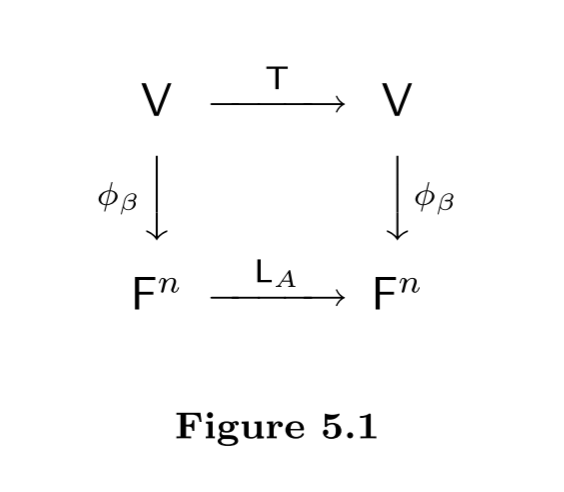
\includegraphics[width=8cm]{images/figure-5-1.png}

Recall that for \(v \in V\), (by \DEF{2.15}) \(\phi_{\beta}(v) = [v]_{\beta}\), the \emph{coordinate vector} of \(v\) \emph{relative to} \(\beta\).

We will show that \(v \in V\) is an eigenvector of \(\T\) corresponding to \(\lambda\) if and only if \(\phi_{\beta}(v)\) is an eigenvector of \(A\) corresponding to \(\lambda\).

Suppose that \(v\) is an eigenvector of \(\T\) corresponding to \(\lambda\).
Then \(v \ne \OV\) and \(\T(v) = \lambda v\) \MAROON{(1)}.
Hence
\begin{align*}
    A \phi_{\beta}(v) & = \LMTRAN_A \phi_{\beta} (v) & \text{by def of left multiplication} \\
        & = \phi_{\beta} \T(v) & \text{by Figure 5.1, the functions ``commute''} \\
        & = \phi_{\beta}(\T(v)) & \text{by def of function composition} \\
        & = \phi_{\beta}(\lambda v) & \text{by \MAROON{(1)}} \\
        & = \lambda \phi_{\beta}(v). & \text{\(\phi_{\beta}\) is linear, in particular}
\end{align*}
And since \(\phi_{\beta}\) is an isomorphism, \(\phi_{\beta}(v) \ne 0 \in F^n\);
hence \(\phi_{\beta}(v)\) is an eigenvector of \(A\) corresponding to \(\lambda\).

Now if \(\phi_{\beta}(v)\) is an eigenvector of \(A\) corresponding to \(\lambda\), then since the argument above is trivially ``reversible'', \(v\) is an eigenvector of \(\T\)
corresponding to \(\lambda\).
(See \EXEC{5.1.14}.)

An equivalent formulation of the result discussed in the preceding paragraph is that for an eigenvalue \(\lambda\) of \(A\) (and hence of \(\T\)),
a vector \(y \in F^n\) is an eigenvector of \(A\) corresponding to \(\lambda\) if and only if \(\phi_{\beta}^{-1}(y)\) is an eigenvector of \(\T\) corresponding to \(\lambda\).

Thus we have \emph{reduced} the problem of finding the eigenvectors \emph{of a linear operator} on a finite-dimensional vector space to the problem of finding the
eigenvectors \emph{of a matrix}.
The next example illustrates this procedure.
\end{remark}

\begin{note}
這邊只是在說,要找一個線性變換的\ eigenvector,可以找這個線性變換「的矩陣代表」的\ eigenvector,該\ vector 其實就是線性變換的某個\ eigenvector 的「座標向量」;
找到該座標向量後把它「轉回」(i.e. 用\ \(\phi_{\beta}^{-1}\) 轉)線性變換的向量即可。
\end{note}

\begin{example} \label{example 5.1.7}
Let \(\T(f(x)) = f(x) + (x + 1)f'(x)\) be the linear operator on \(\POLYRR\) defined in \EXAMPLE{5.1.5},
and let \(\beta\) be the standard ordered basis for \(\POLYRR\).
Recall that \(\T\) has eigenvalues \(1, 2\), and \(3\) and that
\[
    A = [\T]_{\beta} = \begin{pmatrix} 1 & 1 & 0 \\ 0 & 2 & 2 \\ 0 & 0 & 3 \end{pmatrix}.
\]
We consider each eigenvalue separately.

Let \(\lambda_{1}=1\), and define
\
\[
    B_{1}=A-\lambda_{1} I=\left(\begin{array}{lll}
        0 & 1 & 0 \\
        0 & 1 & 2 \\
        0 & 0 & 2
    \end{array}\right).
\]
Then
\[
    x=\left(\begin{array}{l} x_{1} \\ x_{2} \\ x_{3} \end{array}\right) \in \SET{R}^{3}
\]
is an eigenvector corresponding to \(\lambda_{1}=1\) if and only if \(x \ne 0\) and \(x \in \NULL \left( \LMTRAN_{B_{1}} \right)\);
that is, \(x\) is a nonzero solution to the system
\[
    \sysdelim..\systeme{
        x_{2}=0,
        x_{2}+2 x_{3}=0,
        2 x_{3}=0
    }.
\]
Notice that this system has three unknowns, \(x_1, x_2\), and \(x_3\), but one of these, \(x_1\), does not actually appear in the system.
Since the values of \(x_1\) do not affect the system, we assign \(x_1\) a parametric value, say \(x_1 = a\), and solve the system for \(x_2\) and \(x_3\).
Clearly, \(x_2 = x_3 = 0\), and so the eigenvectors \MAROON{of \(A\)} corresponding to \(\lambda_1 = 1\) are of the form
\[
    a \begin{pmatrix} 1 \\ 0 \\ 0 \end{pmatrix} = a e_1
\]
for \(a \ne 0\).
Consequently, the eigenvectors \MAROON{of \(\T\)} corresponding to \(\lambda_1 = 1\) are of the form
\[
    \phi_{\beta}^{-1}\left(a e_{1}\right)=a \phi_{\beta}^{-1}\left(e_{1}\right)=a \cdot 1=a \in \mathcal{P}_2(\SET{R}^2)
\]
for any \(a \ne 0\).
Hence the nonzero constant polynomials are the eigenvectors of \(\T\) corresponding to \(\lambda_1 = 1\).

Next let \(\lambda_2 = 2\), and define
\[
    B_{2}=A-\lambda_{2} I=\left(\begin{array}{lll}
        -1 & 1 & 0 \\
        0 & 0 & 2 \\
        0 & 0 & 1
    \end{array}\right).
\]
It is easily verified that
\[
    \NULL(\LMTRAN_{B_2}) = \left\{ a \begin{pmatrix} 1 \\ 1 \\ 0 \end{pmatrix} : a \in \SET{R} \right\}.
\]
and hence the eigenvectors of \(\T\) corresponding to \(\lambda_2 = 2\) are of the form
\[
    \phi_{\beta}^{-1} \left( a \begin{pmatrix} 1 \\ 1 \\ 0 \end{pmatrix} \right) = a \phi_{\beta}^{-1} (e_1 + e_2) = a (1 + x) = a + x
\]
for \(a \ne 0\).

Finally, consider \(\lambda_{3} = 3\) and
\[
    B_{3}=A-\lambda_{3} I=\left(\begin{array}{rrr}
        -2 & 1 & 0 \\
        0 & -1 & 2 \\
        0 & 0 & 0
    \end{array}\right)
\]
Since
\[
    \NULL\left(\LMTRAN_{B_{3}}\right) = \left\{ a\left(\begin{array}{l} 1 \\ 2 \\ 1 \end{array}\right): a \in \SET{R} \right\},
\]
the eigenvectors of \(\T\) corresponding to \(\lambda_{3}=3\) are of the form
\[
    \phi_{\beta}^{-1}\left(a\left(\begin{array}{l} 1 \\ 2 \\ 1 \end{array}\right)\right)
    = a \phi_{\beta}^{-1}\left(e_{1}+2 e_{2}+e_{3}\right)
    = a \left(1+2 x+x^{2}\right) = a + 2ax + ax^2
\]
for \(a \ne 0\).

For each eigenvalue, select the corresponding eigenvector with \(a = 1 \ne 0\) in the preceding descriptions to obtain \(\gamma = \{ 1, 1 + x, 1 + 2x + x^2 \}\), which is an ordered
basis for \(\POLYRR\) consisting of eigenvectors of \(\T\).
Thus \(\T\) is diagonalizable, and
\[
    [\T]_{\gamma} = \begin{pmatrix} 1 & 0 & 0 \\ 0 & 2 & 0 \\ 0 & 0 & 3 \end{pmatrix}.
\]
\end{example}

We close this section with a \textbf{geometric description} of how a linear operator \(\T\) acts on an eigenvector in the context of a vector space \(V\) over \(\SET{R}\).
(Also see this \href{https://www.youtube.com/watch?v=PFDu9oVAE-g&ab_channel=3Blue1Brown}{video}.)
Let \(v\) be an eigenvector of \(\T\) and \(\lambda\) be the corresponding eigenvalue.
We can think of \(W = \spann(\{ v \})\), the one-dimensional subspace of \(V\) spanned by \(v\), as a line in \(V\) that passes through \(\OV\) and \(v\).
For any \(w \in W, w = cv\) for some scalar \(c\),
and hence
\[
    \T(w) = \T(cv) = c\T(v) = c (\lambda v) = \lambda (c v) = \lambda w;
\]
so \(\T\) acts on the vectors in \(W\) by \textbf{multiplying} each such vector by \(\lambda\).

There are several possible ways for \(\T\) to act on the vectors in \(W\), depending on the value of \(\lambda\).
We consider several cases. (See Figure 5.2.)

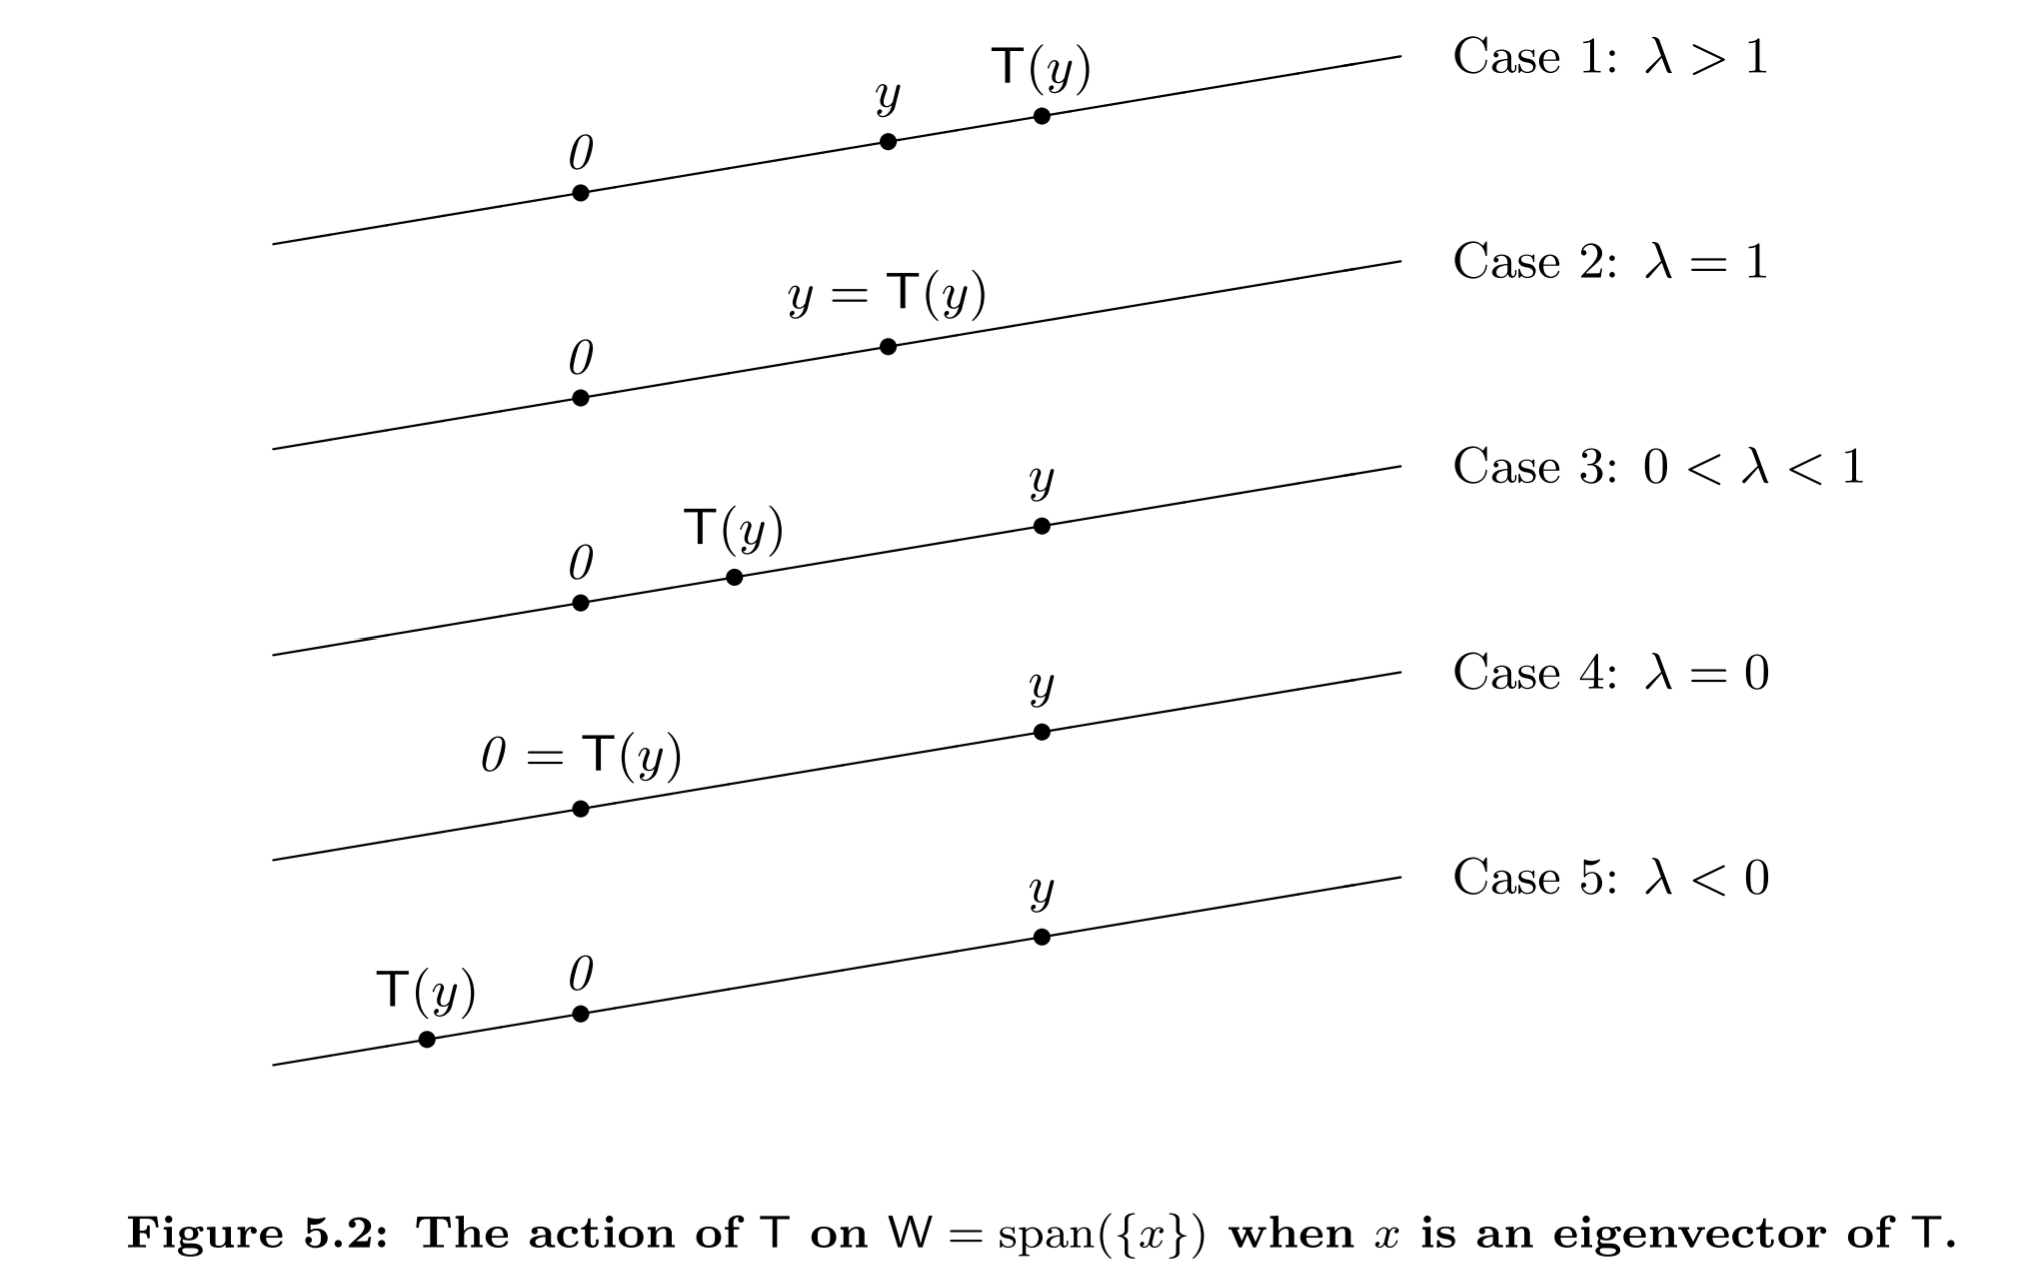
\includegraphics[width=17cm]{images/figure-5-2.png}

\begin{enumerate}
\item[CASE 1.] If \(\lambda > 1\), then \(\T\) moves vectors in \(W\) \emph{farther} from \(\OV\) by a factor of \(\lambda\).
\item[CASE 2.] If \(\lambda = 1\), then \(\T\) acts as the \emph{identity operator} on \(W\).
\item[CASE 3.] If \(\OF < \lambda < 1\), then \(\T\) moves vectors in \(W\) \emph{closer} to \(\OV\) by a factor of \(\lambda\).
\item[CASE 4.] If \(\lambda = \OF\), then \(\T\) acts as the \emph{zero transformation} on \(W\).
\item[CASE 5.] If \(\lambda < \OF\), then \(\T\) \emph{reverses the orientation} of \(W\); that is, \(\T\) moves vectors in \(W\) from one side of \(\OV\) to the other.
\end{enumerate}

To illustrate these ideas, we consider the linear operators in \EXAMPLE{2.1.3}, \EXAMPLE{2.1.4}, and \EXAMPLE{2.1.2}.

For the operator \(\T\) on \(\SET{R}^2\) defined by \(\T(a_1, a_2) = (a_1, -a_2)\), the \emph{reflection} about the \(x\)-axis, \(e_1\) and \(e_2\) are eigenvectors of \(\T\) with corresponding eigenvalues \(1\) and \(-1\), respectively.
Since \(e_1\) and \(e_2\) span the \(x\)-axis and the \(y\)-axis, respectively, \(\T\) \emph{acts as the identity} on the \(x\)-axis and \emph{reverses the orientation}
of the \(y\)-axis.

For the operator \(\T\) on \(\SET{R}^2\) defined by \(\T(a_1, a_2) = (a_1, 0)\), the \emph{projection} on the \(x\)-axis, \(e_1\) and \(e_2\) are eigenvectors of \(\T\) with corresponding eigenvalues \(1\) and \(0\), respectively.
Thus, \(\T\) acts as the identity on the \(x\)-axis and as the \emph{zero operator} on the \(y\)-axis.

Finally, we generalize \EXAMPLE{2.1.2} of this section by considering the operator that \emph{rotates} the plane through the angle, which is defined by
\[
    \T_{\theta}(a_1, a_2) = (a_1 \cos \theta - a_2 \sin \theta, a_1 \sin \theta + a_2 \cos \theta).
\]
Suppose that \(0 < \theta < \pi\).
Then for any nonzero vector \(v\), the vectors \(v\) and \(\T_{\theta}(v)\) are \textbf{not collinear}, and hence \(\T_{\theta}\) maps no one-dimensional subspace of \(\SET{R}^2\) into itself.
But this implies that \(\T_{\theta}\) \emph{has no eigenvectors} and therefore no eigenvalues.
To confirm this conclusion, let \(\beta\) be the standard ordered basis for \(\SET{R}^2\), and note that the \CPOLY{} of \(\T_{\theta}\) is
\[
    \det\left(\left[\T_{\theta}\right]_{\beta}-t I_{2}\right)
    = \det \begin{pmatrix}
        \cos \theta-t & -\sin \theta \\
        \sin \theta & \cos \theta-t
    \end{pmatrix}
    = t^{2} - (2 \cos \theta) t + 1
\]
which has no \textbf{real} zeros because, for \(0 < \theta < \pi\), the discriminant \(4 \cos^2 \theta - 4\) is negative.

\begin{remark} \label{remark 5.1.10}
However, the rotation operator in the previous discussion \emph{does have} eigenvalues when the field is \emph{complex number}, and \(\pm \iu\) are the eigenvalue of this transformation.
In addition, the ``geometric explanation'' in the discussion no longer applies, since it does not correctly describe the ``geometry'' of complex number.
\end{remark}

\section{Diagonalizability} \label{sec 5.2}
\section{Matrix Limits and Markov Chains} \label{sec 5.3}

\TODOREF{Enhance this bloody hell section when finishing \SEC{7.2}, since the core theorems here depend on that section.}

In this section, we apply what we have learned thus far in \CH{5} to study the \emph{limit} of a sequence of \emph{powers} \(A, A^2, ..., A^n, ...\),
where \(A\) is a square matrix \RED{with \emph{complex} entries}.
(That is, many derived theorems require that the given matrix is over the complex number.)
Such sequences and their limits have practical applications in the natural and social sciences.

\begin{additional definition} \label{adef 5.2}
We \emph{assume familiarity with limits of sequences of real numbers}.
(Refer to some real analysis book.)
The limit of a sequence of \emph{complex} numbers \(\{ z_m : m = 1, 2, ... \}\) can be \emph{defined} in terms of the limits of the sequences of the \emph{real} and \emph{imaginary parts}:
If \(z_m = r_m + \iu s_n\), where \(r_m\) and \(s_m\) are real numbers, and \(\iu\) is the imaginary number such that \(\iu^2 = -1\), then
\[
    \lim_{m \toINF} z_m = \lim_{m \toINF} r_m + \iu \lim_{m \toINF} s_m, 
\]
provided that \(\lim_{m \toINF} r_m\) and \(\lim_{m \toINF} s_m\) exist.
\end{additional definition}

\begin{definition} \label{def 5.10}
Let \(L, A_1, A_2, ...\) be \(n \X p\) matrices having \emph{complex} entries.
The sequence \(A_1, A_2, ...\) is said to \textbf{converge} to the \(n \X p\) matrix \(L\), called the \textbf{limit} of the sequence, if
\[
    \lim_{m \toINF} (A_m)_{ij} = L_{ij}
\]
for all \(1 \le i \le n\) and \(1 \le j \le p\).
To denote that \(L\) is the limit of the sequence, we write
\[
    \lim_{m \toINF} (A_m) = L.
\]
\end{definition}

\begin{note}
這個定義就是把矩陣的極限的存在,reduce 到個別\ entry 的極限的存在,也就是複數\ sequence 的極限的存在;
而根據\ \ADEF{5.2},複數\ sequence 的極限的存在又\ reduce 到(兩個)實數\ sequence 的極限的存在。
然後作者假設讀者知道實數\ sequence 極限存在的定義。
\end{note}

\begin{note}
It seems that calculating limit of sequence of complex numbers require other techniques;
refer to some Complex Analysis course.
\end{note}

\begin{example} \label{example 5.3.1}
If
\[
    A_m = \begin{pmatrix}
        1 - \frac{1}{m} & \left( - \frac{3}{4} \right)^m & \frac{3m^2}{m^2 + 1} + \iu \left( \frac{2m + 1}{m - 1} \right) \\
        \RED{\left( \frac{\iu}{2} \right)^m} & 2 & \left( 1 + \frac{1}{m} \right)^m
    \end{pmatrix}
\]
then by the definition of the limit of sequence of complex numbers, sequence of real numbers, (and Calculus)
\[
    \lim_{m \toINF} A_m = \begin{pmatrix}
        1 & 0 & 3 + 2\iu \\
        0 & 2 & e
    \end{pmatrix},
\]
where \(e\) is the base of the natural algorithm.
\end{example}

\begin{note}
For the red highlight part, see some \href{https://math.stackexchange.com/questions/898296/the-limit-of-complex-sequence}{reference}.
We have
\begin{align*}
    \frac{\abs{\iu}}{\abs{2}} & = \frac{1}{2} & \text{using \DEF{d.3}} \\
        & < 1,
\end{align*}
hence \(\lim_{m \toINF} \left( \cfrac{\abs{\iu}}{\abs{2}} \right)^m = 0\) \MAROON{(1)} \quad by the calculation of sequence of \emph{real} numbers.
And we have
\begin{align*}
    \lim_{m \toINF} \left| \left( \frac{\iu}{2} \right)^m \right|
        & = \lim_{m \toINF} \left( \frac{\abs{\iu}}{\abs{2}} \right)^m & \text{using the solution in the reference} \\
        & = 0 & \text{by \MAROON{(1)}}
\end{align*}
So the absolute value of of the value we want is \(0\), which implies the value we want is also \(0\).
\end{note}

\begin{remark} \label{remark 5.3.1}
A simple, but important, property of matrix limits is contained in the next theorem.
Note the \emph{analogy} with the familiar property of limits of sequences of \emph{real} numbers that asserts that if \(\lim_{m \toINF} a_m\) exists, then
\[
    \lim_{m \toINF} c a_m = c \lim_{m \toINF} a_m.
\]
The next theorem is similar to this fact.
\end{remark}

\begin{theorem} \label{thm 5.11}
Let \(A_1, A_2, ...\) be a sequence of \(n \X p\) matrices with complex entries such the that it converges to the matrix \(L\).
Then for any \(P \in M_{r \X n}(\SET{C})\) and \(Q \in M_{p \X s}(\SET{C})\),
\[
    \lim_{m \toINF} PA_m = P \lim_{m \toINF} A_m = PL \quad \text{ and } \lim_{m \toINF} A_m Q = \left[\lim_{m \toINF} A_m\right] Q = LQ.
\]
\end{theorem}

\begin{proof}
For any \(i (1 \le i \le r)\) and \(j (1 \le j \le p)\),
\begin{align*}
    \lim_{m \toINF} (PA_m)_{ij} & = \lim_{m \toINF} \sum_{k = 1}^n P_{ik} (A_m)_{kj} & \text{by def of matrix multiplication} \\
        & = \sum_{k = 1}^n \lim_{m \toINF} P_{ik} (A_m)_{kj} & \text{change order of limit and summation,} \\
        & & \text{since summation is finite and limit of each term exists} \\
        & = \sum_{k = 1}^n P_{ik} \lim_{m \toINF} (A_m)_{kj} & \text{move ``constant'' out of limit} \\
        & = \sum_{k = 1}^n P_{ik} \cdot L_{kj} & \text{by supposition} \\
        & = (PL)_{ij}. & \text{by def of matrix multiplication}
\end{align*}
Hence \(\lim_{m \toINF} PA_m = PL\).
The proof that \(\lim_{m \toINF} A_m Q = LQ\) is similar.
\end{proof}

\begin{corollary} \label{corollary 5.11.1}
Let \(A \in M_{n \X n}(\SET{C})\) be such that \(\lim_{m \toINF} A^m = L\).
(\(A^m\) is just the \(m\)th power of \(A\).)
Then for any \emph{invertible} matrix \(Q \in M_{n \X n}(\SET{C})\),
\[
    \lim_{m \toINF} (Q A Q^{-1})^m = Q \left[ \lim_{m \toINF} A^m \right] Q^{-1} = Q L Q^{-1}.
\]
\end{corollary}

\begin{proof}
Since
\[
    (Q A Q^{-1})^m = (Q A Q^{-1})(Q A Q^{-1})...(Q A Q^{-1}) = Q A^m Q^{-1},
\]
we have
\begin{align*}
    \lim_{m \toINF} (Q A Q^{-1})^m & = \lim_{m \toINF} Q A^m Q^{-1} & \text{by what we have shown} \\
        & = Q \left[ \lim_{m \toINF} A^m Q^{-1} \right] & \text{by applying \THM{5.11}} \\
        & = Q \left[\lim_{m \toINF} A^m \right] Q^{-1} & \text{by applying \THM{5.11} again} \\
        & = Q L Q.
\end{align*}
\end{proof}

\begin{remark} \label{remark 5.3.2}
In the discussion that follows, we frequently encounter the set
\[
    S = \{ \lambda \in \SET{C}: \abs{\lambda} < 1 or \lambda = 1 \}.
\]
\emph{Geometrically}, this set consists of the complex number \(1\) and the \emph{interior} of the \emph{unit disk}
(the disk of radius \(1\) centered at the origin).
This set is of interest because if \(\lambda\) is a complex number, then \textbf{\(\lim_{m \toINF} \lambda^m\) exists if and only \(\lambda \in S\)}.
This fact, which is obviously true if \(\lambda\) is real, can be shown to be true for complex numbers also.

The following theorem gives \emph{necessary and sufficient conditions} for the existence of the type of limit under consideration.
\end{remark}

\begin{note}
若只看「圓盤」跟實數軸的交集,那個交集內的實數其實也是那些取\ power 後極限存在的實數。
也就是\ \((-1, 1]\) 區間。
\end{note}

\begin{theorem} \label{thm 5.12}
Let \(A\) be a square matrix with complex entries.
Then \(lim_{m \toINF} A^m\) exists if and only if \textbf{both} of the following conditions bold.
\begin{enumerate}
\item Every \emph{eigenvalue} of \(A\) is contained in \(S\) (see \RMK{5.3.2}).
\item If \(1\) is an eigenvalue of \(A\), then the \emph{dimension} of the eigenspace corresponding to \(1\) equals the \emph{algebraic multiplicity} of \(1\) as an eigenvalue of \(A\).
\end{enumerate}
\end{theorem}

\begin{proof}
\RED{Warning: the proof of part(b) needs some other facts in later chapters}.

For part(b), there are two proofs of theorem, but one proof of this theorem, which relies on the theory of \emph{Jordan canonical forms} (\SEC{7.2}), can be found in \EXEC{7.2.19}.
A second proof, which makes use of Schur's theorem (\THM{6.14}), can be found in the article by the author :)

The \textbf{necessity} of condition (a) is easily justified.
For suppose that \(\lambda\) is an eigenvalue of \(A\) such that \(\lambda \RED{\notin} S\).
Let \(v\) be an eigenvector of \(A\) corresponding to \(\lambda\).
Regarding \(v\) as an \(n \X 1\) \emph{matrix}, we see that
\begin{align*}
    \lim_{m \toINF} (A^m v) & = \left( \lim_{m \toINF} A^m \right) v & \text{by \THM{5.11}} \\
        & = Lv,
\end{align*}
where \(L = \lim_{m \toINF} A^m\).
But we also have \(\lim_{m \toINF} (A^mv) = \lim_{m \toINF} \lambda^m v)\) by \EXEC{5.1.16}(b),
but the right side diverges because \(\lim \lambda^m\) does not exist. (Since \(\lambda \notin S\)!)
So \(\lim_{m \toINF} (A^mv)\) does not exist, and we get a contradiction.
So \(\lambda\) must be in \(S\).

Hence if \(\lim_{m \toINF} A^m\) exists, then condition (a) of \THM{5.12} must hold.
\end{proof}

\begin{remark} \label{remark 5.3.3}
Currently, we still cannot prove the \textbf{necessity} of condition (b),
that is, if \(\lim_{m \toINF} A^m\), exists, then condition (a) of \THM{5.12} must hold.

Furthermore, we cannot prove that if condition(a)(b) of \THM{5.12} hold, then \(\lim_{m \toINF} A^m\) exists.

Although we are unable to prove the necessity of condition \((b)\) here, we consider an example such that when (b) fails. then the limit of matrix power does not exist.

Observe that the \CPOLY{} for the matrix
\[
    B = \begin{pmatrix} 1 & 1 \\ 0 & 1 \end{pmatrix}
\]
is \((t - 1)^2\), and hence \(B\) has eigenvalue \(\lambda = 1\) with algebraic multiplicity \(2\).
It can easily be verified that \(\dim(\lambda) = 1\), so that condition (b) of \THM{5.12} is violated.
A simple mathematical induction argument can be used to show that
\[
    B^m = \begin{pmatrix} 1 & m \\ 0 & 1 \end{pmatrix},
\]
and therefore that \(\lim_{m \toINF} B^m\) does not exist.
We see in \CH{7} that if \(A\) is a matrix for which condition (b) \emph{fails}, then \(A\) is \emph{similar to} a matrix whose \emph{upper left \(2 \X 2\) submatrix} is precisely this matrix \(B\).
\end{remark}

In most of the applications involving matrix limits, the matrix is \emph{diagonalizable}, and so (by \THM{5.8}(a),) condition (b) of \THM{5.12} is automatically satisfied.
In this case, \THM{5.12} \emph{reduces to} the following theorem, which can be proved using our previous results.

\begin{theorem} \label{thm 5.13}
Let \(A \in M_{n \X n}(\SET{C})\) satisfy the following two conditions.
\begin{enumerate}
\item[(i)] Every eigenvalue of \(A\) is contained in \(S\) (see \RMK{5.3.2}).
\item \(A\) is diagonalizable.
\end{enumerate}
Then \(\lim_{m \toINF} A^m\) exists.
\end{theorem}

\begin{note}
注意這證明是完全獨立於\ \THM{5.12} 的。
\end{note}

\begin{proof}
Since \(A\) is diagonalizable, there exists an invertible matrix \(Q\) such that \(Q^{-1} A Q = D\) is a diagonal matrix.
(Hence \(A = Q D Q^{-1}\).)
Suppose that
\[
    D = \begin{pmatrix}
        \lambda_1 & 0 & ... & 0 \\
        0 & \lambda_2 & ... & 0 \\
        \vdots & \vdots & & \vdots \\
        0 & 0 & ... & \lambda_n
    \end{pmatrix}.
\]
Because \(\lambda_1, \lambda_2, ... , \lambda_n\) are the eigenvalues of \(A\), condition (i) requires that for each \(i\),
\(\lambda_i \in S\) (see \RMK{5.3.2}), that is, either \(\lambda_i = 1\) or \(\abs{\lambda_i} < 1\).
Thus
\begin{equation*}
    \lim_{m \toINF} \lambda_i^m = \begin{cases}
        1 \quad \text{ if } \lambda_i = 1 \\
        0 \quad \text{ otherwise.}
    \end{cases}
\end{equation*}
But since
\[
    D^m = \begin{pmatrix}
        \lambda_1^m & 0 & ... & 0 \\
        0 & \lambda_2^m & ... & 0 \\
        \vdots & \vdots & & \vdots \\
        0 & 0 & ... & \lambda_n^m
    \end{pmatrix},
\]
the sequence \((D^m)\) converges, and let it converge to \(L\).
Then we have
\begin{align*}
    \lim_{m \toINF} A^m & = \lim_{m \toINF} (Q D Q^{-1})^m & \text{of course} \\
        & = Q L Q^{-1} & \text{by \CORO{5.11.1}}
\end{align*}
\end{proof}

The technique for computing \(\lim_{m \toINF} A^m\) used in the proof of \THM{5.13} can be employed in actual computations, as we now illustrate.
Let
\[
    A = \begin{pmatrix}
        \frac{7}{4} & -\frac{9}{4} & -\frac{15}{4} \\
        \frac{3}{4} & \frac{7}{4}  & \frac{3}{4} \\
        \frac{3}{4} & -\frac{9}{4}  & -\frac{11}{4} \\
    \end{pmatrix}.
\]
Using the methods in \SEC{5.1} and \SEC{5.2}, we obtain
\[
    Q = \begin{pmatrix}
        1 & 3 & -1 \\
        -3 & -2 & 1 \\
        2 & 3 & -1
    \end{pmatrix}
    \quad \text{ and } \quad
    D = \begin{pmatrix}
        1 & 0 & 0 \\
        0 & -\frac{1}{2} & 0 \\
        0 & 0 & \frac{1}{4}
    \end{pmatrix}
\]
such that \(Q^{-1} A Q = D\).
Hence
\begin{align*}
    \lim_{m \toINF} A^m & = \lim_{m \toINF} (Q D Q^{-1})^m = \lim_{m \toINF} Q D^m Q^{-1} = Q (\lim_{m \toINF} D^m) Q^{-1} \\
        & \quad \quad \quad \text{(just the process in the proof of \THM{5.13})} \\
        & = \begin{pmatrix}
                1 & 3 & -1 \\
                -3 & -2 & 1 \\
                2 & 3 & -1
            \end{pmatrix}
            \left[
                \lim_{m \toINF}
                \begin{pmatrix}
                    1 & 0 & 0 \\
                    0 & \left( -\frac{1}{2} \right)^m & 0 \\
                    0 & 0 & \left( \frac{1}{4} \right)^m
                \end{pmatrix}
            \right]
            \begin{pmatrix}
                -1 & 0 & 1 \\
                -1 & 1 & 2 \\
                -5 & 3 & 7
            \end{pmatrix} \\
        & = \begin{pmatrix}
                1 & 3 & -1 \\
                -3 & -2 & 1 \\
                2 & 3 & -1
            \end{pmatrix}
            \begin{pmatrix}
                1 & 0 & 0 \\
                0 & 0 & 0 \\
                0 & 0 & 0
            \end{pmatrix}
            \begin{pmatrix}
                -1 & 0 & 1 \\
                -1 & 1 & 2 \\
                -5 & 3 & 7
            \end{pmatrix} \\
        = \begin{pmatrix}
                -1 & 0 & 1 \\
                3 & 0 & -3 \\
                -2 & 0 & 2
            \end{pmatrix}.
\end{align*}

Next, we consider an application that uses the limit of powers of a matrix.
Suppose that the population of a certain metropolitan area \emph{remains constant} but there is a \emph{continual movement} of people between the city and the suburbs.
Specifically, let the entries of the following matrix \(A\) represent the probabilities that someone living in the city or in the suburbs on January 1 will be living in each region on January 1 \emph{of the next year}.

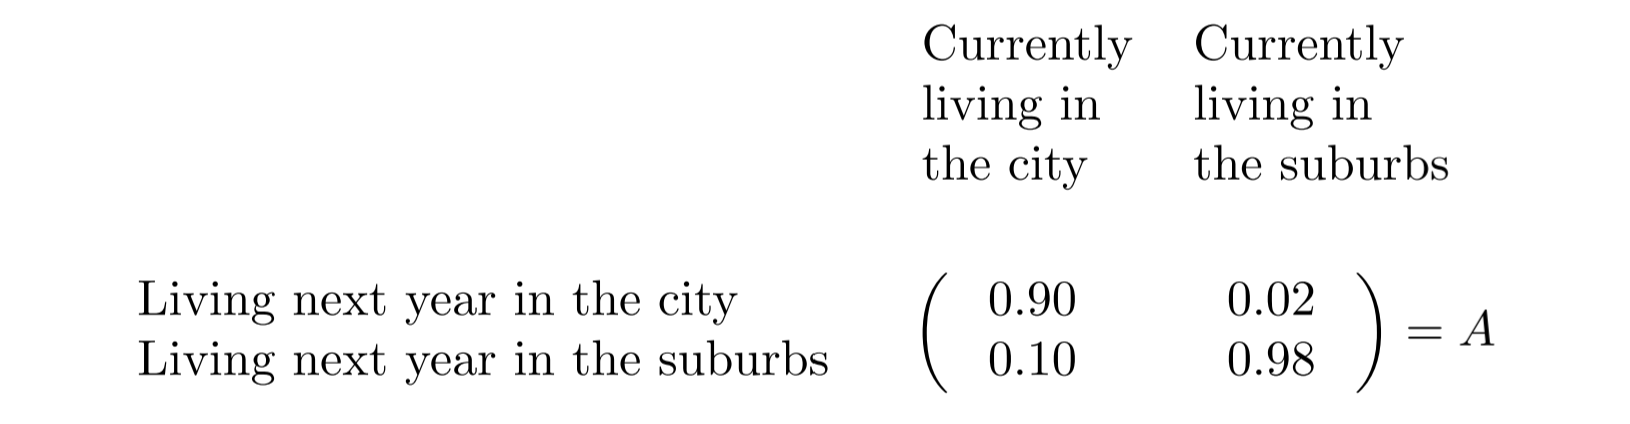
\includegraphics[width=16cm]{images/5-3-city-suburb-movement.png}

For instance, the probability that someone living in the city (on January 1) will be living in the suburbs next year (on January 1) is \(0.10\).
Notice that since the entries of \(A\) are \textbf{probabilities}, they are \textbf{nonnegative}.
Moreover, the \emph{assumption of a constant population} in the metropolitan area requires that \emph{the sum of the entries of each \textbf{column} of \(A\) be \(1\)}.

\begin{additional definition} \label{adef 5.3}
Any square matrix having these two properties (nonnegative entries and columns that sum to \(1\)) is called a \textbf{transition matrix} or a \textbf{stochastic matrix}.
For an arbitrary \(n \X n\) transition matrix \(M\), the rows and columns correspond to \(n\) \textbf{states}, and the entry \(M_{ij}\) represents the probability of moving from state \(j\) to state \(i\) in one \textbf{stage}.
(Note the reversed order of \(ij\)-entry and \(j\)-to-\(i\) movement.)

The \textbf{probability vector} is a vector that has nonnegative entries that sum to \(1\).
Note that each column of a transition matrix is a probability vector.
\end{additional definition}

In our example, there are two states (residing in the city and residing in the suburbs).
So, for example, \(A_{21}\) is the probability of moving from the city to the suburbs in one stage, that is, in one year.
We now determine the probability that a city resident will be living in the suburbs \emph{after \(2\) years}.
There are \emph{two different ways} in which such a move can be made:
remaining in the city for 1 year and then moving to the suburbs, or moving to the suburbs during the first year and remaining there the second year.
(See Figure 5.3.)

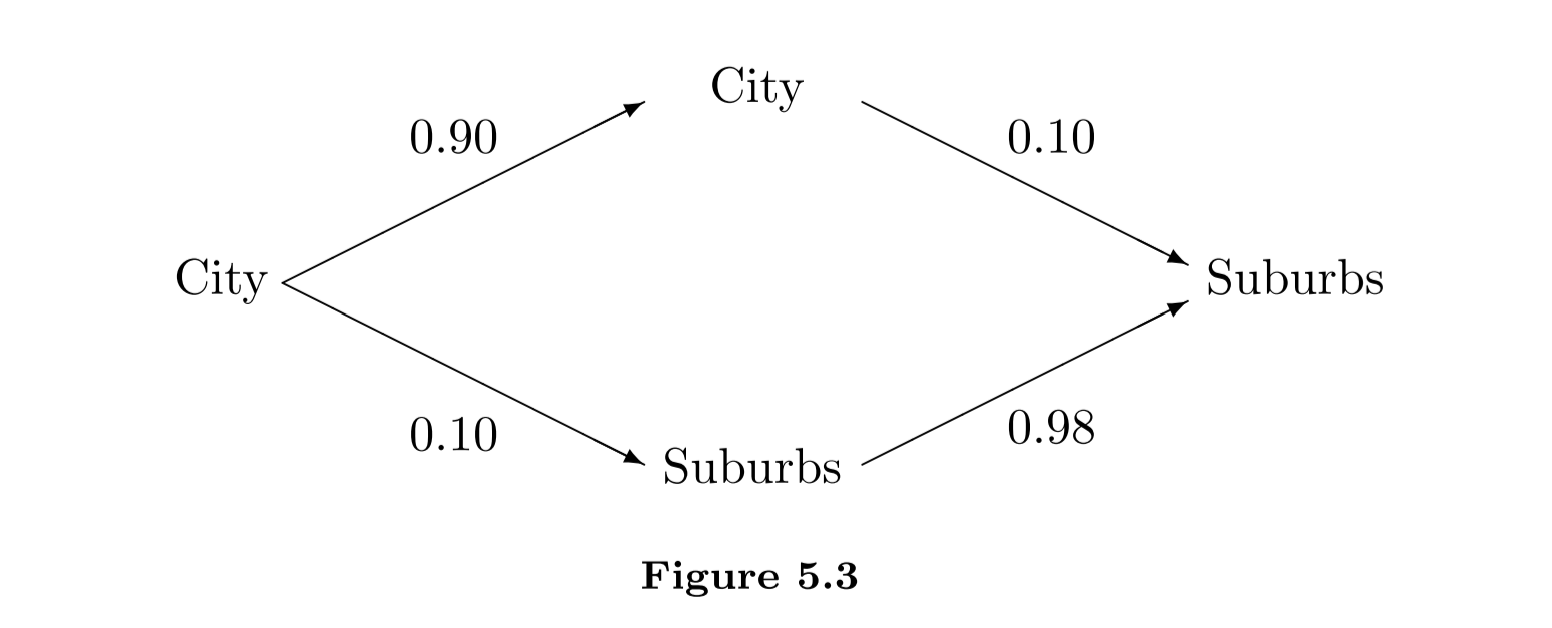
\includegraphics[width=16cm]{images/figure-5-3.png}

The probability that a city dweller remains in the city for the first year is \(0.90\), whereas the probability that the city dweller moves to the suburbs during the first year is \(0.10\).
Hence the probability that a city dweller stays in the city for the first year and then moves to the suburbs during the
second year is the \emph{product} \((0.90)(0.10)\).
Likewise, the probability that a city dweller moves to the suburbs in the first year and remains in the suburbs during the second year is the product \((0.10)(0.98)\).
Thus the probability that a city dweller will be living in the suburbs after 2 years is the \emph{sum of these products}, \((0.90)(0.10) + (0.10)(0.98) = 0.1\).
Observe that this number is \emph{obtained by the same calculation as that which produces \((A^2)_{21}\)},
and hence \((A^2)_{21}\) represents the probability that a city dweller will be living in the suburbs after 2 years.
In general, for any transition matrix \(M\), the entry \((M^m)_{ij}\) represents the probability of moving from state \(j\) to state \(i\) in \(m\) stages.

Suppose additionally that in year 2000, 70\% of the population of the metropolitan area lived in the city and 30\% lived in the suburbs.
We record these data \emph{as a column vector}:

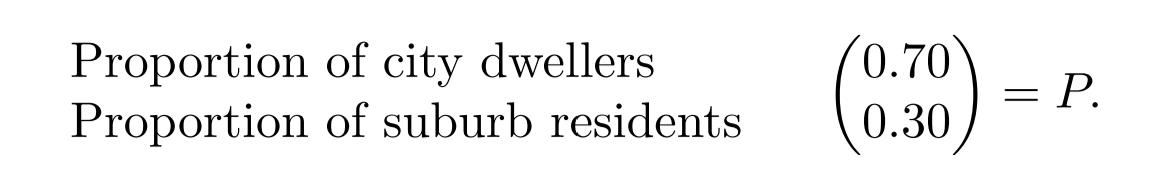
\includegraphics[width=14cm]{images/5-3-city-suburb-prob-vector-1.png}

Notice that the rows of \(P\) correspond to the states of residing in the city and residing in the suburbs, respectively,
and that these \emph{states are listed in the same order as the listing in the transition matrix} \(A\).
Observe also that the column vector \(P\) \emph{contains nonnegative entries that sum to \(1\)};
such a vector is called a \textbf{probability vector}.
In this terminology, \emph{each column of a transition matrix is a probability vector}.
It is often convenient to regard the entries of a transition matrix or a probability vector as \emph{proportions or percentages instead of probabilities}, as we have already done with the probability vector \(P\).

In the vector \(AP = \begin{pmatrix} 0.636 \\ 0.364 \end{pmatrix}\), the first coordinate is the sum \((0.90)(0.70) + (0.02)(0.30)\).
The first term of this sum, \((0.90)(0.70)\), represents the proportion of the 2000 metropolitan population that \emph{remained in the city} during the next year,
and the second term, \((0.02)(0.30)\), represents the proportion of the 2000 metropolitan population that \emph{moved into the city} (from the suburb) during the next year.
Hence the first coordinate of \(AP\) represents the proportion of the metropolitan population that was living in the city in 2001.
Similarly, the second coordinate of \(AP\), represents the proportion of the metropolitan population that was living in the suburbs in 2001.
This argument can be \emph{easily extended} to show that the coordinates of
\[
    A^P = A(AP) = \begin{pmatrix} 0.57968 \\ 0.42032 \end{pmatrix}
\]
represent the proportions of the metropolitan population that were living in each location in 200\RED{2}.
In general, the coordinates of \(A^m P\) represent the \emph{proportion} of the metropolitan population that will be living in the city and suburbs, respectively, after \(m\) stages (\(m\) years after 2000).

From the value of \(AP\) and \(A^2 P\), or just from the value of the entries of \(A\), it seems that the proportion of the population living in cities is getting smaller.
\textbf{Will the city eventually \emph{be depleted} if this trend continues?}
In view of the preceding discussion, it is \emph{natural to define the eventual proportion} of the city dwellers and suburbanites \emph{to be the first and second coordinates, respectively, of} \(\lim_{m \toINF} A^m P\).
We now compute this limit.
It is easily shown that \(A\) is diagonalizable, and so there is an invertible matrix \(Q\) and a diagonal matrix \(D\) such that \(Q^{-1} A Q = D\).
In fact,
\[
    Q = \begin{pmatrix}
        \cfrac{1}{6} & -\cfrac{1}{6} \\ \cfrac{5}{6} & \cfrac{1}{6}
    \end{pmatrix}
    \quad \text{ and }
    D = \begin{pmatrix}
        1 & 0 \\ 0 & 0.88
    \end{pmatrix}.
\]
Therefore (using the process in the proof of \THM{5.13},)
\[
    L = \lim_{m \toINF} A^m = \lim_{m \toINF} Q D^m Q^{-1}) = Q \begin{pmatrix} 1 & 0 \\ 0 & 0 \end{pmatrix} Q^{-1} =
    \begin{pmatrix}
        \cfrac{1}{6} & \cfrac{1}{6} \\ \cfrac{5}{6} & \cfrac{5}{6}
    \end{pmatrix}
\]
Consequently, (by \THM{5.11})
\[
    \lim_{m \toINF} A^m P = LP = \begin{pmatrix}
        \cfrac{1}{6} \\ \cfrac{5}{6}
    \end{pmatrix}
\]
Thus, eventually, \(\frac{1}{6}\) of the population will live in the city and \(\frac{5}{6}\) will live in the suburbs each year.
Note that the vector \(LP\) satisfies \(A (LP) = LP  = 1 \cdot LP\).
Hence \(LP\) is \textbf{both a probability vector} and \textbf{an eigenvector of \(A\)} corresponding \textbf{to the eigenvalue \(1\)}. Since the eigenspace of \(A\) corresponding to the eigenvalue \(1\) is one-dimensional (just by calculation),
there is only one such vector \(L\), that is, the vector that is an eigenvector of \(A\) corresponding to the eigenvalue \(1\) and sums its entries to \(1\) is \emph{unique}.
And \(LP\) is \textbf{independent of the initial choice} of probability vector \(P\).
(See \EXEC{5.3.15}.)
For example, had the 2000 metropolitan population consisted entirely of city dwellers, the
limiting outcome would be the same.

\begin{remark} \label{remark 5.3.4}
In analyzing the city suburb problem, we gave \emph{probabilistic interpretations} of \(A^2\) and \(AP\), showing that \(A^2\) is a transition matrix and \(AP\) is a probability vector.
In fact, the product of any two transition matrices \emph{is} a transition matrix, and the product of any transition matrix and probability vector \emph{is} a probability vector.
A proof of these facts is a simple corollary of the next theorem, which characterizes transition matrices and probability
vectors.
\end{remark}

\begin{theorem} \label{thm 5.14}
Let \(M\) be an \(n \X n\) matrix having \emph{real nonnegative} entries, let \(v\) be a column vector in \(\SET{R}^n\) having nonnegative coordinates, and let \(u \in \SET{R}^n\) be the column vector in which \emph{each coordinate equals \(1\)}.
Then
\begin{enumerate}
\item \(M\) is a transition matrix if and only if \(u^\top M = u^\top\);
\item \(v\) is a probability vector if and only if \(u^\top v = (1)\).
\end{enumerate}
\end{theorem}

\begin{proof}
See \EXEC{5.3.16}.
\end{proof}

\begin{corollary} \label{corollary 5.14.1} \ 

\begin{enumerate}
\item The product of two \(n \X n\) transition matrices is an \(n \X n\) transition matrix.
In particular, any power of a transition matrix is a transition matrix.

\item The product of a transition matrix and a probability vector is a probability vector.
\end{enumerate}
\end{corollary}

\begin{proof}
See \EXEC{5.3.16}.
\end{proof}

\begin{remark} \label{remark 5.3.5}
The city-suburb problem is \emph{an example of a process} in which elements of a set are each \emph{classified as being in one of several fixed states} that \emph{can switch over time}.
In general, such a process is called a \textbf{stochastic process}.
The switching to a particular state is described by a probability, and \emph{in the most general case}, this probability depends on such factors as the state in question, the \emph{time} in question, some or all of the \emph{previous states} in which the object has been (including the current state), and the states that \emph{other objects} are in or have been in.

(For instance, the object could be an American voter, and the state of the object could be his or her preference of political party.
In this example, all four of the factors mentioned above influence the probability that an object is in a particular state at a particular time.)

If, however, the probability that an object in one state \(A\) changes to a different state \(B\) \emph{in a fixed interval of time} depends only on the two states \(A\) and \(B\) (and not on the time, earlier states, or other factors), then the stochastic process is called a \textbf{Markov process}.
If, in addition, the number of possible states is \emph{finite}, then the Markov process is called a \textbf{Markov chain}.
We treated the city suburb example as a two-state Markov chain.
Of course, a Markov process is usually only an idealization of reality because the probabilities involved are almost never constant over time.

Note that some literature defines Markov chain as a Markov process and having \emph{countable} states.
\end{remark}

(Skip another example in page 290 to 292.)

In the preceding two examples, we saw that \(\lim_{m \toINF} A^m P\), where \(A\) is the transition matrix and \(P\) is the initial probability vector of the Markov chain, gives the eventual proportions in each state.
In general, however, \textbf{the limit of powers of a transition matrix need not exist}.
For example, if
\[
    M = \begin{pmatrix} 0 & 1 \\ 1 & 0 \end{pmatrix},
\]
then \(\lim_{m \toINF} M^m\) does not exist because odd powers of \(M\) equal \(M\) and even powers of \(M\) equal \(I\).
The reason that the limit fails to exist is that \textbf{condition (a) of \THM{5.12} does not hold for \(M\)} (\(-1\) is an eigenvalue, but \(-1 \notin S\) where \(S\) is defined in \RMK{5.3.2}).
In fact, it can be shown (see \EXEC{7.2.20}) that \textbf{the only transition matrices} \(A\) such that \(\lim_{m \toINF} A^m\) does not exist are precisely those matrices for which condition (a) of \THM{5.12} fails to hold.

But even if the limit of powers of the transition matrix exists, the computation of the limit may be quite difficult.
(The reader is encouraged to work \EXEC{5.3.6} to appreciate the truth of the last sentence.)
Fortunately, there is a large and important class of transition matrices for which this limit exists and is easily computed -- this is the class of \textbf{regular transition matrices}.

\begin{definition} \label{def 5.11}
A transition matrix is called \textbf{regular} if \emph{some power} of the matrix contains only nonzero (i.e., positive) entries.
\end{definition}

\begin{example} \label{example 5.3.2}
The transition matrix
\[
    \begin{pmatrix} 0.90 & 0.02 \\ 0.10 & 0.98 \end{pmatrix}
\]
of the Markov chain used in the city-suburb problem is clearly regular because each entry is positive.
On the other hand, the transition matrix
\[
    A = \begin{pmatrix}
        1 & 0.4 & 0.1 & 0 \\
        0 & 0.3 & 0.5 & 0 \\
        0 & 0 & 0.2 & 0 \\
        0 & 0.3 & 0.2 & 1
    \end{pmatrix}
\]
is not regular because the first column of \(A^m\) is
\[
    \begin{pmatrix} 1 \\ 0 \\ 0 \\ 0 \end{pmatrix}
\]
for any power \(m\).

Observe that a regular transition matrix \emph{may contain zero entries}.
For example,
\[
    M = \begin{pmatrix} 0.9 & 0.5 & 0 \\ 0 & 0.5 & 0.4 \\ 0.1 & 0 & 0.6 \end{pmatrix}
\]
is regular because every entry of \(M^2\) is positive.
\end{example}

\begin{remark} \label{remark 5.3.6}
The remainder of this section is devoted to proving that, for a \textbf{regular} transition matrix \(A\), the \emph{limit} of the sequence of powers of \(A\) exists and \textbf{has identical columns}.
From this fact, it is easy to compute this limit.
In the course of proving this result, we \emph{obtain some interesting bounds for the magnitudes of eigenvalues of any square matrix}.
These bounds are given in terms of the sum of the absolute values of the rows and columns of the matrix.
The necessary terminology is introduced in the definitions that follow.
\end{remark}

\begin{definition} \label{def 5.12}
Let \(A \in M_{n \X n}(\SET{C})\).
For \(1 \le i, j \le n\), define \(\rho_i(A)\) to be the sum of the \emph{absolute values} of the entries of row \(i\) of \(A\), and define \(\nu(A)\) to be equal to the sum of the absolute values of the entries of column \(j\) of \(A\).
Thus
\[
    \rho_i(A) = \sum_{j = 1}^n \abs{A_{ij}} \quad \text{for} i = 1, 2, ..., n
\]
and
\[
    \nu_j(A) = \sum_{i = 1}^n \abs{A_{ij}} \quad \text{for} j = 1, 2, ..., n.
\]
The \textbf{row sum} of \(A\), denoted \(\rho(A)\), and the \textbf{column sum} of \(A\), denoted \(\nu(A)\), are defined as
\[
    \rho(A) = \max \{ \rho_i(A) : 1 \le i \le n \} \quad \text{ and } \quad \nu(A) = \max \{ \nu_j(A) : 1 \le j \le n \}.
\]
\end{definition}

\begin{example} \label{example 5.3.3}
For the matrix
\[
    A = \begin{pmatrix}
        1 & -\iu & 3-4\iu \\
        -2+\iu & 0 & 6 \\
        3 & 2 & \iu
    \end{pmatrix}
\]
\(\rho_1(A) = 7, \rho_2(A) = 6 + \sqrt{5}, \rho_3(A) = 6, \nu_1(A) = 4 + \sqrt{5}, \nu_2(A) = 3\), and  \(\nu_3(A) = 12\).
Hence \(\rho(A) = 6 + \sqrt{5}\) and \(\nu(A) = 12\).
\end{example}

Our next results show that the \emph{smaller} of \(\rho(A)\) and \(\nu(A)\) is an \textbf{upper bound for the absolute values of eigenvalues of \(A\).} 
In the preceding example, for instance, \(A\) has no eigenvalue with absolute value greater than \(6 + \sqrt{5}\).

To obtain a \emph{geometric view} of the following theorem, we introduce some terminology.
\begin{additional definition}
For an \(n \X n\) matrix \(A\), we define the \(i\)th \textbf{Gershgorin disk} \(C_i\) to be the \emph{disk in the complex plane} with center \(A_{ii}\) and radius \(r_i = \rho_i(A) - \abs{A_{ii}}\);
that is
\[
    C_i = \{ z \in \SET{C} : \abs{z - A_{ii}} \le r_i \}.
\]
\end{additional definition}

For example, consider the matrix
\[
    A = \begin{pmatrix} 1 + 2 \iu & 1 \\ 2 \iu & -3 \end{pmatrix}.
\]
For this matrix, \(C_1\) is the disk with center \(1 + 2\iu\) and radius \(1\), and \(C_2\) is the disk with center \(-3\) and radius \(2\).
(See Figure 5.4)

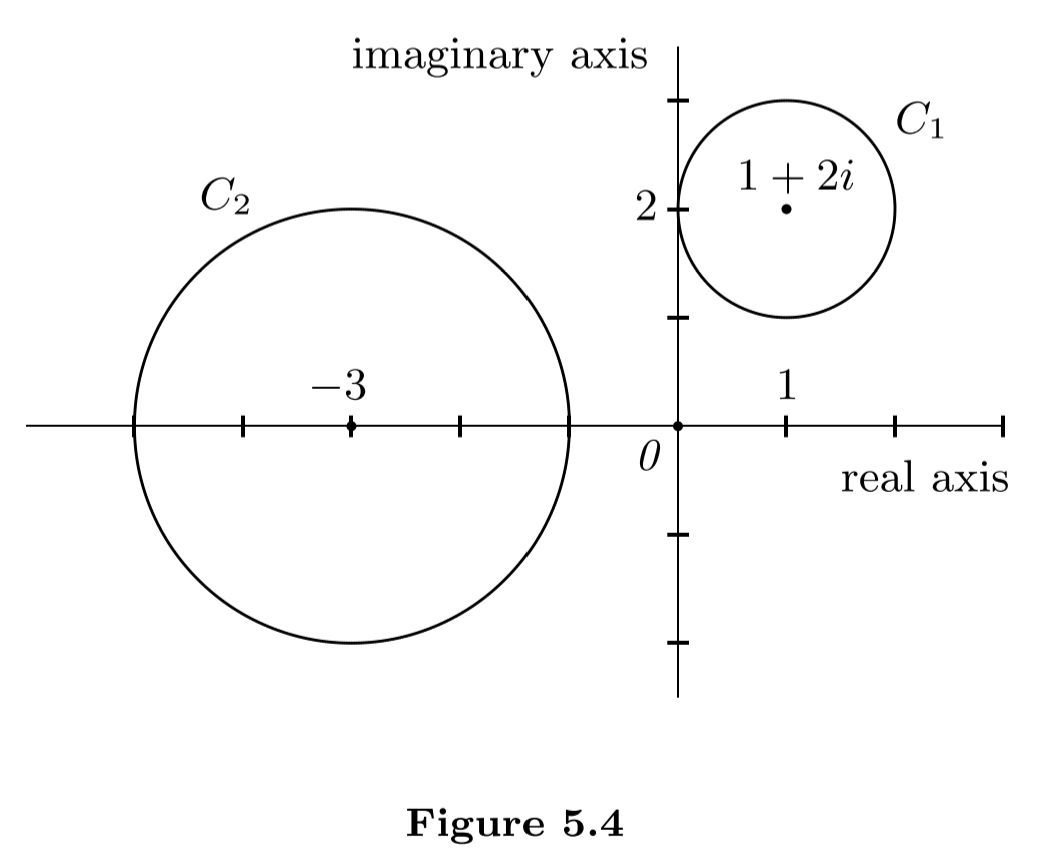
\includegraphics[width=14cm]{images/figure-5-4.png}

Gershgorin's circle theorem, stated below, tells us that all the eigenvalues of \(A\) are located within these two disks.
In particular, we see that \(0\) is \emph{not} an eigenvalue, and hence by \EXEC{5.1.9}(c), \(A\) is invertible.

\begin{theorem} [Gershgorin's Circle Theorem] \label{thm 5.15}
Let \(A \in M_{n \X n}(\SET{C})\).
Then every eigenvalue of \(A\) is contained in a Gersbgorin disk.
\end{theorem}

\begin{proof}
Let \(\lambda\) be an eigenvalue of \(A\) with the corresponding eigenvector
\[
    v = \begin{pmatrix} v_1 \\ v_2 \\ \vdots \\ v_n \end{pmatrix}.
\]
Then \(v\) satisfies the matrix equation \(Av = \lambda v\), which can be written as
\[
    \sum_{j = 1}^n A_{ij} v_j = \lambda v_i \text{for \(1 \le i \le n\)}. \quad \quad \quad \MAROON{(1)}
\]
Suppose that \(v_k\) is a coordinate of \(v\) having the \emph{largest absolute value}; \MAROON{(2)} \quad \quad
note that since \(v\) is an eigenvector, \(v \ne \OV\), hence some coordinate \(v_i\) is nonzero, which implies \(v_k \ne 0\). \MAROON{(3)} \quad \quad
We show that \(\lambda\) \textbf{lies in \(C_k\)}, that is, \(\abs{\lambda - A_{kk}} \le r_k\).
(We will do some trick: multiply \(\abs{v_k}\) in the both sides of this to-be-proved inequality.)
For \(i = k\), it follows from \(\MAROON{(1)}\) that
\begin{align*}
    \abs{v_k}\abs{\lambda - A_{kk}} & = \abs{(v_k)(\lambda - A_{kk})} & \text{by \THM{d.3}(a)} \\
        & = \abs{\lambda v_k - A_{kk} v_k} & \text{of course} \\
        & = \left| \sum_{j = 1}^n A_{kj} v_j - A_{kk} v_k \right| & \text{by \MAROON{(1)}} \\
        & = \left| \sum_{j \ne k} A_{kj} v_j \right| & \text{of course} \\
        & \le \sum_{j \ne k} \abs{ A_{kj} } \abs{ v_j } & \text{by \THM{d.3}(c)} \\
        & \le \sum_{j \ne k} \abs{ A_{kj} } \abs{ v_{\RED{k}} } & \text{by \MAROON{(2)}} \\
        & = \abs{v_k} \sum_{j \ne k} \abs { A_{kj} } & \text{move ``constant'' out of summation} \\
        & = \abs{v_k} r_k. & \text{by def of \(r_k\)}
\end{align*}
Thus we have \(\abs{v_k}\abs{\lambda - A_{kk}} \le \abs{v_k} r_k\).
And since by \MAROON{(3)}, \(\abs{v_k} > 0\), hence (by cancellation law) we have \(\abs{\lambda - A_{kk}} \le r_k\).
\end{proof}

\begin{corollary} \label{corollary 5.15.1}
Let \(\lambda\) be any eigenvalue of \(A \in M_{n \X n}(\SET{C})\).
Then \(\abs{lambda} \le \rho(A)\).
\end{corollary}

\begin{proof}
By Gershgorin's circle theorem, \(\abs{\lambda - A_{kk}} \le r_k\) for some \(k\). \MAROON{(1)} \quad \quad
Hence
\begin{align*}
    \abs{\lambda} & = \abs{(\lambda - A_{kk}) + A_{kk}} & \text{of course} \\
        & \le \abs{\lambda - A_{kk}} + \abs{A_{kk}} & \text{by \THM{d.3}(c)} \\
        & \le r_k + \abs{A_{kk}} & \text{by \MAROON{(1)}} \\
        & = \rho_k(A) & \text{by \DEF{5.12}} \\
        & \le \rho(A). & \text{by definition}
\end{align*}
\end{proof}

\begin{note}
這個\ Corollary 的意義是,eigenvalue 的絕對值會小於等於矩陣的行和。
\end{note}

\begin{corollary} \label{corollary 5.15.2}
Let \(\lambda\) be any eigenvalue of \(A \in M_{n \X n}(\SET{C})\).
Then
\[
    \abs{\lambda} \le \min \{ \rho(A), \nu(A) \}.
\]
\end{corollary}

\begin{proof}
Since \(\abs{\lambda} \le \rho(A)\) by \(1\), it suffices to show that \(\abs{\lambda} \le \nu(A)\).
By \EXEC{5.1.15}, \(\lambda\) is an eigenvalue of \(A^\top\), and so \(\abs{\lambda} \le \rho(A^\top)\) by \CORO{5.15.1}.
But the rows of \(A^\top\) are the columns of \(A\); consequently \(\rho(A^\top) = \nu(A)\).
Therefore \(\abs{\lambda} \nu(A)\).
\end{proof}

The next corollary is immediate from \CORO{5.15.2}
\begin{corollary} \label{corollary 5.15.3}
If \(\lambda\) is an eigenvalue of a \emph{transition} matrix, then \(\abs{\lambda} \le 1\).
(Since each column of a transition matrix sums to \(1\).)
\end{corollary}

\begin{theorem} \label{thm 5.16}
Every \emph{transition} matrix has \(1\) as an eigenvalue.
\end{theorem}

\begin{proof}
Let \(A\) be an \(n \X n\) \emph{transition} matrix, and let \(u \in \SET{R}^n\) be the column vector in which \emph{each coordinate is \(1\)}.
Then \(A^\top u = u\) by \THM{5.14}, and hen\(c\)e \(u\) is an eigenvector of \(A^\top\) corresponding to the eigenvalue \(1\). But since \(A\) and \(A^\top\) have the same eigenvalues, it follows that \(1\) is also an eigenvalue of \(A\).
\end{proof}

Suppose that \(A\) is a transition matrix for which some eigenvector corresponding to the eigenvalue \(1\) \emph{has only nonnegative coordinates}.
Then some multiple of this vector is \emph{a probability vector} \(P\) as well as an eigenvector of \(A\) corresponding to eigenvalue \(1\).
It is interesting to \emph{observe}(i.e. not proved yet) that if \(P\) is the initial probability vector of a Markov chain having \(A\) as its transition matrix, then the Markov chain is \emph{completely static}.
(That is, in particular, \(AP = P\).)
For in this situation, \(A^m P = P\) for every positive integer \(m\); hence the probability of being in each state never
changes.
Consider, for instance, the city suburb problem with
\[
    P = \begin{pmatrix} \cfrac{1}{6} \\ \cfrac{5}{6} \end{pmatrix}.
\]

\begin{theorem} \label{thm 5.17}
Let \(A \in M_{n \X n}(\SET{C})\) be a matrix in which each entry is a positive real number, and let \(\lambda\) be a \emph{complex} eigenvalue of \(A\) such that \(\abs{\lambda} = \rho(A)\).
Then \(\lambda = \rho(A)\) and \(\{ u \}\) is a basis for \(E_{\lambda}\), where \(u \in C^n\) is the column vector in which each coordinate equals \(1\).
\end{theorem}

\begin{note}
That is, given a ``positive'' matrix \(A\), if \(\lambda\) is an eigenvalue and equal to the row sum of \(A\), then \(\lambda\) is in fact also positive.
\end{note}

\begin{proof}
Let \(v\) be an \emph{arbitrary} eigenvector of \(A\) corresponding to \(\lambda\), with coordinates \(v_1, v_2, ..., v_n\).
Suppose that \(v_k\) is the coordinate of \(v\) having the \emph{largest absolute value}, and let \(b = \abs{v_k}\). \MAROON{(b.0)}

Then
\begin{align*}
    \rho(A) b & = \abs{\lambda} b & \text{by supposition} \\
        & = \abs{\lambda} \abs{v_k} & \text{by \MAROON{(b.0)}} \\
        & = \abs{\lambda v_k} & \text{by \THM{d.3}(a)} \\
        & = \left| \sum_{j = 1}^n A_{kj} v_j \right| & \text{in particular from the fact \(Av = \lambda v\)} \\
        &\ \RED{\le} \sum_{j = 1}^n \abs{ A_{kj} v_j } & \text{by \THM{d.3}(c)} \\
        & = \sum_{j = 1}^n \abs{A_{kj}} \abs{v_j} & \text{by \THM{d.3}(a)} \\
        &\ \RED{\le} \sum_{j = 1}^n \abs{A_{kj}} \abs{v_{\RED{k}}} = \sum_{j = 1}^n \abs{A_{kj}} b & \text{since \(\abs{v_k}\) is the largest and \MAROON{(b.0)}} \\
        & = \rho_k(A) b & \text{by def of \(\rho_k(A)\)} \\
        &\ \RED{\le} \rho(A) b \quad \quad \quad \MAROON{(1)} & \text{by def of \(\rho(A)\)}.
\end{align*}
So the three inequalities in the derivation above are actually equalities; that is,
\begin{enumerate}
\item \(\left| \sum_{j = 1}^n A_{kj} v_j \right| \RED{=} \sum_{j = 1}^n \abs{ A_{kj} v_j }\),
\item \(\sum_{j = 1}^n \abs{A_{kj}} \abs{v_j} \RED{=} \sum_{j = 1}^n \abs{A_{kj}} b\), and
\item \(\rho_k(A) b \RED{=} \rho(A)\).
\end{enumerate}

We will see in \EXEC{6.1.15}(b) that (a) holds if and only if all the terms \(A_{kj} v_j (j = 1, 2, ... , n)\) are obtained by multiplying some nonzero complex number \(z\) by nonnegative \textbf{real} numbers.
(That is, intuitively, (a) holds, if and only if all these complex numbers are \textbf{parallel and have same direction} in the complex plane.)
Without loss of generality, we assume that \(\abs{z} = 1\). \MAROON{(b.2)}
Thus there exist nonnegative real numbers \(c_1, c_2, ..., c_n\) such that
\[
    A_{kj} v_j = c_j z. \quad \quad \quad \MAROON{(2)}
\]
By (b) and the assumption (that each entry is a positive real number, so) that \(A_{kj} \ne 0\) for all \(k\) and \(j\), we have
\[
    \abs{v_j} = \abs{v_k} = b \text{ for } j = 1, 2, ..., n. \quad \quad \quad \MAROON{(3)}
\]

%根據假設,所有 \(\abs{v_j}\) 都小於等於 \(\abs{v_k}\)。若這時真的有一個 \(\abs{v_j}\) 是 "小於" \(\abs{v_k}\),則 \(\sum_{j = 1}^k \abs{v_j}\) 就一定小於 \(\sum_{j = 1}^n \abs{v_k} = \sum_{j = 1}^n b\)。連帶的,(b) 會是錯的,矛盾。

Combining \MAROON{(2)} and \MAROON{(3)}, we obtain that for \(j = 1, 2, ..., n\),
\begin{align*}
    b & = \abs{v_k} & \text{by \MAROON{(b.0)}} \\
      & = \left| \frac{c_j}{A_{kj}} z \right| & \text{by \MAROON{(2)}}\\
      & = \left| \frac{c_j}{A_{kj}} \right| \abs{z} = \left| \frac{c_j}{A_{kj}} \right| & \text{by \MAROON{(b.2)}} \\
      & = \frac{c_j}{A_{kj}}, & \text{since \(c_j, A_{kj}\) are nonnegative}
\end{align*}
and therefore, by \MAROON{(2)}, we have \(v_j = \cfrac{c_j}{A_{kj}} z = b z\) for all \(j\).
So
\[
    v = \begin{pmatrix} v_1 \\ v_2 \\ \vdots \\ v_n \end{pmatrix}
    = \begin{pmatrix} bz \\ bz \\ \vdots \\ bz \end{pmatrix}
    = bz \begin{pmatrix} 1 \\ 1 \\ \vdots \\ 1 \end{pmatrix}
    = bzu,
\]
(since \(v\) is arbitrary), hence \(\{ u \}\) is a basis for \(E_{\lambda}\).

Finally, observe that all of the entries of \(A_u\) are positive because the same is true for the entries of both \(A\) and \(u\).
But \(Au = \lambda u\), and hence \(\lambda > 0\).
Therefore, \(\lambda = \abs{\lambda} = \rho(A)\).
\end{proof}

\begin{corollary} \label{corollary 5.17.1}
Let \(A \in M_{n \X n}(\SET{C})\) be a matrix in which each entry is positive, and let \(\lambda\) be an eigenvalue of \(A\) such that \(\abs{\lambda} = \nu(A)\).
Then \(\lambda = \nu(A)\), and the dimension of \(E_{\lambda}\) equals \(1\).
\end{corollary}

\begin{proof}
See \EXEC{5.3.17}.
\end{proof}

\begin{corollary} \label{corollary 5.17.2}
Let \(A \in M_{n \X n}(\SET{C})\) be a \emph{transition matrix} in which each entry is positive, and let \(\lambda\) be any eigenvalue of \(A\) other than \(1\).
Then \(\abs{\lambda} < 1\).
Moreover, the eigenspace corresponding to the eigenvalue \(1\) has dimension \(1\).
\end{corollary}

\begin{proof}
See \EXEC{5.3.17}.
\end{proof}

Our next result extends \CORO{5.17.2} to \emph{regular transition} matrices and thus shows that regular transition matrices satisfy condition (a) of \THM{5.12} and \THM{5.13}.

\begin{theorem} \label{thm 5.18}
Let \(A\) be a \emph{regular transition} matrix, and let \(\lambda\) be an eigenvalue of \(A\).
Then
\begin{enumerate}
\item \(\abs{\lambda} \le 1\).
\item If \(\lambda = 1\), then \(\lambda = 1\), and \(\dim(E_{\lambda}) = 1\).
\end{enumerate}
\end{theorem}

\begin{proof} \ 

\begin{enumerate}
\item This was proved as \CORO{5.15.3}.
\item Since \(A\) is regular, there exists a positive integer \(s\) such that \(A^s\) has only positive entries.
Because \(A\) is a transition matrix and the entries of \(A^s\) are positive, the entries of \(A^{s+1} = A^s(A)\) are positive.
Suppose that \(\abs{\lambda} = 1\).
Then (by \EXEC{5.1.16}(b)) \(\lambda^s\) and \(\lambda^{s+1}\) are eigenvalues of \(A^s\) and \(A^{s + 1}\), respectively, having absolute value \(1\).
So by \CORO{5.17.2}, \(\lambda^s = \lambda^{s+1} = 1\).
Thus \(\lambda = 1\).
Let \(E_{\lambda}\). and \(E'_{\lambda}\) denote the eigenspaces of \(A\) and \(A^s\), respectively, corresponding to \(\lambda = 1\).
Then (of course, trivially, from definition,) \(E_{\lambda} \subseteq E'_{\lambda}\);
and, by \CORO{5.17.2}, \(\dim(E'_{\lambda}) = 1\).
Hence \(E_{\lambda} = E'_{\lambda}\), and \(\dim(E_{\lambda}) = 1\).
\end{enumerate}
\end{proof}

\begin{corollary} \label{corollary 5.18.1}
Let \(A\) be a \emph{regular transition} matrix that is \emph{diagonalizable}.
Then \(\lim_{m \toINF} A^m\) exists.
\end{corollary}

\begin{remark} \label{remark 5.3.7}
The preceding corollary, which follows \emph{immediately from \THM{5.18} and \THM{5.13}}, is not the best possible result.
In fact, it can be shown that (in holy \SEC{7.2}) if \(A\) is a regular transition matrix, then the algebraic multiplicity of \(1\) as an eigenvalue of \(A\) is \(1\).
Thus, by \THM{5.7}, condition (b) of \THM{5.12} is satisfied.
So if \(A\) is a \emph{regular transition} matrix, \textbf{\(\lim_{m \toINF} A^m\) exists regardless of whether \(A\) is or is not diagonalizable}.
As with \THM{5.12}, however, the fact that the algebraic multiplicity of \(\lambda = 1\) as an eigenvalue of \(A\) is \(1\) \textbf{cannot be proved at this time}.
Nevertheless, we state this result here (leaving the proof until \EXEC{7.2.21}) and deduce further facts about \(\lim A^m\) when \(A\) is a regular transition matrix.
\end{remark}

\begin{theorem} \label{thm 5.19}
Let \(A\) be a \textbf{regular transition} matrix.
Then
\begin{enumerate}
\item The multiplicity of \(1\) as an eigenvalue of \(A\) is \(1\).
\item \(\lim_{m \toINF} A^m\) exists.
\item \(L = \lim_{m \toINF} A^m\) is a transition matrix.
\item \(AL = LA = L\).
\item The columns of \(L\) are identical.
In fact, each column of \(L\) is equal to \emph{the unique probability vector} \(v\) that is \emph{also an eigenvector} of \(A\) corresponding to the eigenvalue \(1\).
\item For any probability vector \(w\), \(\lim_{m \toINF} (A^m w) = v\).
\end{enumerate}
\end{theorem}

\begin{proof} \ 

\begin{enumerate}
\item See \EXEC{7.2.21}.
\item This follows from part (a) and \THM{5.18} and \THM{5.12}.

\item By \THM{5.14}, we must show that \(u^\top L = u^\top\).
Now \(A^m\) is a transition matrix by the \CORO{5.14.1}, so
\[
    u^\top L = u^\top \lim_{m \toINF} A^m = \lim_{m \toINF} u^\top A^m = \lim_{m \toINF} u^\top = u^\top,
\]
and it follows that \(L\) is a transition matrix.
\item By \THM{5.11},
\[
    AL = A \lim_{m \toINF} A^m = \lim_{m \toINF} A A^m = \lim_{m \toINF} A^{m + 1} = L.
\]
Similarly, \(LA = L\).

\item Since \(AL = L\) by part(d), each column of \(L\) is an eigenvector of \(A\) corresponding to the eigenvalue \(1\).
(Why? See \THM{2.13}(a).)
Moreover, by part(c), each column of \(L\) is a probability vector.
Thus, by part(a), each column of \(L\) is equal to the unique probability vector \(v\) corresponding to the eigenvalue \(1\) of \(A\).

\item Let \(w\) be any probability vector, and set \(y = \lim_{m \toINF} A^m w = L w\).
Then \(y\) is a probability vector by the \CORO{5.14.1}, and also \(A y = A L w = L w = y\) by part(d).
Hence \(y\) is also an eigenvector corresponding to the eigenvalue \(1\) of A.
So \(y = v\) by part(e).
\end{enumerate}
\end{proof}

\begin{definition}
The vector \(v\) in \THM{5.19}(e) is called the \textbf{fixed probability vector} or \textbf{stationary vector} of the regular transition matrix \(A\).
\end{definition}



\section{Invariant Subspaces and the Cayley-Hamilton Theorem} \label{sec 5.4}

In \SEC{5.1}, we observed that if \(v\) is an eigenvector of a linear operator \(\T\), then \(\T\) maps the span of \(\{ v \}\) into itself.
Subspaces that are mapped into themselves are of great importance in the study of linear operators (see, e.g., \EXEC{2.1.29}--\EXEC{2.1.33}).

\begin{definition} \label{def 5.14}
Let \(\T\) be a linear operator on a vector space \(V\).
A subspace \(W\) of \(V\) is called a \textbf{\(\T\)-invariant subspace} of \(V\) if \(\T(W) \subseteq W\), that is, if
\(\T(v) \in W\) for all \(v \in W\).
\end{definition}

\begin{example} \label{example 5.4.1}
Suppose that \(\T\) is a linear operator on a vector space \(V\).
Then the following subspaces of \(V\) are \(\T\)-invariant:
\begin{enumerate}
\item[1.] \(\{ \OV \}\)
\item[2.] \(V\)
\item[3.] \(\RANGET\)
\item[4.] \(\NULLT\)
\item[5.] \(E_{\lambda}\), for any eigenvalue \(\lambda\) of \(\T\).
\end{enumerate}

For 5., see \EXEC{5.4.3}, for other items, see \EXEC{2.1.29}.
\end{example}

\begin{example} \label{example 5.4.2}
Let \(\T\) be the linear operator on \(\SET{R}^3\) defined by
\[
    \T(a, b, c) = (a + b, b + c, 0).
\]
Then the \(xy\)-plane = \(\{ (x, y, 0): x, y \in \SET{R} \}\) and the \(x\)-axis = \(\{ (x, 0, 0): x \in \SET{R}\}\) are (some examples of) \(\T\)-invariant subspaces of \(\SET{R}^3\).
\end{example}

\begin{additional definition} \label{adef 5.5}
Let \(\T\) be a linear operator on a vector space \(V\), and let \(x\) be a \emph{nonzero} vector in \(V\).
The subspace \(W = \spann(\{ x, \T(x), \T^2(x), ... \})\) is called the \textbf{\(\T\)-cyclic subspace of \(V\) generated by \(x\)}.
It is a simple matter to show that \(W\) is \(\T\)-invariant.

Note that we do not require \(V\) to be finite-dimensional.
\end{additional definition}

\begin{remark} \label{remark 5.4.1}
In fact, \(W\) is the ``smallest'' \(\T\)-\emph{invariant subspace} of \(V\) containing \(x\).
That is, any \(\T\)-invariant subspace of \(V\) containing \(x\) must also contain \(W\) (see \EXEC{5.4.11}).
Cyclic subspaces have various uses.
We apply them in this section to establish the Cayley Hamilton theorem.
In \EXEC{5.4.31}, we outline a method for using cyclic subspaces to \emph{compute the \CPOLY{}} of a linear operator \textbf{without resorting to determinants}.
Cyclic subspaces also play an important role in \CH{7}, where we study matrix representations of non-diagonalizable linear operators.
\end{remark}

\begin{example} \label{example 5.4.3}
Let \(\T\) be the linear operator on \(\SET{R}^3\) defined by
\[
    \T(a, b, c) = (-b + c, a + c, 3c).
\]
We determine the \(\T\)-cyclic subspace generated by \(e_1 = (1, 0, 0)\).
Since
\[
    \T(e_1) = \T(1, 0, 0) = (0, 1, 0) = e_2
\]
and
\[
    \T^2(e_1) = \T(\T(e_1)) = \T(e_2) = (-1, 0, 0) = -e_1,
\]
it follows that
\[
    \spann(\{ e_1, \T(e_1), \T^2(e_1), ... \}) = \spann(\{ e_1, e_2 \}) = \{ (s, t, 0) : s, t \in \SET{R} \}.
\]
\end{example}

\begin{example} \label{example 5.4.4}
Let \(\T\) be the linear operator on \(\mathcal{P}(\SET{R})\) defined by \(\T(f(x)) = f'(x)\).
Then the \(\T\)-cyclic subspace generated by \(x^2\) is (of course!) \(\spann(\{ x^2, 2x, 2 \}) = \mathcal{P}_2(\SET{R})\).
\end{example}

\begin{remark} \label{remark 5.4.2}
The existence of a \(\T\)-invariant subspace provides the opportunity to define a new linear operator \textbf{whose domain is this subspace}.
If \(\T\) is a linear operator on \(V\) and \(W\) is a \(\T\)-invariant subspace of \(V\), then the \emph{restriction} \(\T_W\) of \(\T\) to \(W\) (see Appendix B, page 545) is a mapping \emph{from \(W\) to \(W\)}, and it follows that \(\T_W\) is a linear operator on \(W\) (see \EXEC{5.4.7}, or \EXEC{2.1.30}).
As a linear operator, \(\T_W\) \emph{inherits certain properties} from its parent operator \(\T\).
The following result illustrates one way in which the two operators are linked.
\end{remark}

\begin{theorem} \label{thm 5.20}
Let \(\T\) be a linear operator on a finite-dimensional vector space \(V\), and let \(W\) be a \(\T\)-invariant subspace of \(V\).
Then the \CPOLY{} of \(\T_W\) \textbf{divides} the \CPOLY{} of \(\T\).
\end{theorem}

\begin{proof}
Choose an ordered basis \(\gamma = \{ v_1, v_2, ..., v_k \}\) \emph{for \(W\)}, and \emph{extend} it to an ordered basis \(\beta = \{ v_1, v_2, ... v_k, v_{k + 1}, ..., v_n \}\) for \(V\).
Let \(A = [\T]_{\beta}\) and \(B_1 = [\T_W]_{\gamma}\).
Then, by \EXEC{5.4.12}, \(A\) can be written in the form
\[
    A = \begin{pmatrix}
        \RED{B_1} & B_2 \\ O & B_3
    \end{pmatrix}.
\]
Let \(f(t)\) be the \CPOLY{} of \(\T\) and \(g(t)\) the \CPOLY{} of \(\T_W\).
Then
\[
    f(t) = \det(A - tI_n) = \begin{pmatrix} B_1 - t I_{\RED{k}} & B_2 \\ O & B_3 - t I_{\RED{n - k}} \end{pmatrix}
    = g(t) \cdot \det(B_3 - t I_{n - k})
\]
by \EXEC{4.3.21}.
Thus \(g(t)\) divides \(f(t)\).
\end{proof}

\begin{example} \label{example 5.4.5}
Let \(\T\) be the linear operator on \(\SET{R}^4\) defined by
\[
    \T(a, b, c, d) = (a + b + 2c - d, b + d, 2c - d, c + d),
\]
and let \(W = \{ (t, s, 0, 0) : t, s \in \SET{R} \}\).
Observe that \(W\) is a \(\T\)-invariant subspace of \(\SET{R}^4\) because, for any vector \((a, b, 0, 0) \in W\),
\[
    \T(a, b, 0, 0) = (a + b, b, 0, 0) \in W.
\]
Let \(\gamma = \{ e_1, e_2 \}\), which is an ordered basis for \(W\).
Extend \(\gamma\) to the \emph{standard} ordered basis \(\beta\) for \(\SET{R}^4\).
Then
\[
    B_1 = [\T_W]_{\gamma} = \begin{pmatrix} 1 & 1 \\ 0 & 1 \end{pmatrix}
    \quad \text{ and } \quad
    A = [\T]_{\beta} = \begin{pmatrix} 1 & 1 & 2 & -1 \\ 0 & 1 & 0 & 1 \\ 0 & 0 & 2 & -1 \\ 0 & 0 & 1 & 1 \end{pmatrix}
\]
in the notation of \THM{5.20}.
Let \(f(t)\) be the \CPOLY{} of \(\T\) and \(g(t)\) be the \CPOLY{} of \(\T_W\).
Then
\begin{align*}
    f(t) & = \det(A - tI_4) = \det \begin{pmatrix} 1-t & 1 & 2 & -1 \\ 0 & 1-t & 0 & 1 \\ 0 & 0 & 2-t & -1 \\ 0 & 0 & 1 & 1-t \end{pmatrix} & \text{by definition} \\
         & = \det \begin{pmatrix} 1-t & 1 \\ 0 & 1-t \end{pmatrix} \cdot \det \begin{pmatrix} 2-t & -1 \\ 1 & 1-t \end{pmatrix} & \text{by \EXEC{4.3.21}} \\
         & = g(t) \cdot \det \begin{pmatrix} 2-t & -1 \\ 1 & 1-t \end{pmatrix} & \text{by \THM{5.20}}
\end{align*}
\end{example}

\begin{remark} \label{remark 5.4.3}
In view of \THM{5.20}, we may use the \CPOLY{} of \(T_W\) to \emph{gain information} about the \CPOLY{} \emph{of \(\T\) itself}.
In this regard, cyclic subspaces are useful because the \CPOLY{} of the restriction of a linear operator \(\T\) to a cyclic subspace is \emph{readily computable}.
(See the theorem below.)
\end{remark}

\begin{theorem} \label{thm 5.21}
Let \(\T\) be a linear operator on a \textbf{finite}-dimensional vector space \(V\), and let \(W\) denote the \(\T\)-cyclic subspace of \(V\) generated by a nonzero vector \(v \in V\).
Let \(k = \dim(W)\).
Then
\begin{enumerate}
\item \(\beta = \{ v, \T(v), \T^2(v), ..., \T^{\RED{k - 1}}(v) \}\) is a \textbf{basis} for \(W\).
\item If \(\T_{\RED{k}}(v) = -a_0 v - a_1 \T(v) - ... - a_{k - 1} \T^{k - 1}(v) \), then the \CPOLY{} oF \(\T_W\) is \(f(t) = (-1)^k (t^k + a_{k - 1} t^{k-1} + ... + a_1 t + a_0).\).

(That is, If we write \(\T_{\RED{k}}(v)\) as a linear combination \(\beta\), but without loss of generality and a negative sign in these coefficient \(a_i\), we can derive the \CPOLY{} of \(\T_W\) use these coefficients \(a_i\).)
\end{enumerate}
\end{theorem}

\begin{proof} \ 

\begin{enumerate}
\item Since \(v \ne \OV\), the set \(\{ v \}\) is \LID{}.
Let \(j\) be the \emph{largest positive} integer for which
\[
    \beta = \{ v, \T(v), ..., \T^{j - 1}(v) \}
\]
is linearly independent.
Such \(j\) must exist since \(V\) is finite-dimensional (hence any \LID{} set must be finite).
Let \(Z = \spann(\beta)\).
Then \(\beta\) is a generating set for \(Z\) and is \LID{}, hence is a basis for \(Z\).
Furthermore, since by definition of \(j\), \(\beta \cup \{ \T^j(v) \}\) is \LDP{}, \(\T^j(v) \in \spann(\beta)\) by \THM{1.7}.
That is, \(\T^j(v) \in Z\).
We use this information to show that \(Z\) is a \(\T\)-invariant subspace of \(V\).

Let \(w \in Z\).
Since \(w\) is a linear combination of the vectors of \(\beta\), there exist scalars \(b_0, b_1, ..., b_{j - 1}\) such that
\[
    w = b_0 v + b_1 \T(v) + ... + b_{j - 1} \T^{j - 1}(v),
\]
and hence (by applying \(\T\) on both sides,)
\begin{align*}
    \T(w) & = \T(b_0 v + b_1 \T(v) + ... + b_{j - 1} \T^{j - 1}(v)) \\
          & = b_0 \T(v) + b_1 \T^2(v) + ... + b_{j - 2} \T^{\RED{j - 1}}(v) + b_{j - 1} \T^{\RED{j}}(v), & \text{since \(\T\) is linear}
\end{align*}
where \(\T(v), ..., \T^{\RED{j - 1}}(v)\) belong to the bases \(\beta\), and \(\T^{\RED{j}}(v) \in Z\), thus \(\T(w)\) is still a linear combination of vectors in \(Z\), and hence belong to \(Z\).
So \(Z\) is \(\T\)-invariant.
Furthermore, \(v \in Z\) (since \(v \in \beta\)).
By \EXEC{5.4.11}, \(W\) is the \emph{smallest} \(\T\)-invariant subspace of \(V\) that contains \(v\), so that \(W \subseteq Z\).
Clearly, \(Z \subseteq W\) (since \(Z = \spann(\{ v, \T(v), ..., \T^{j - 1}(v) \})\) but \(W = \spann(\{ v, \T(v), ... \})\)), and so we conclude that \(Z = W\).
It follows that \(\beta\) is a basis for \(W\), and therefore \(\dim(W) = j\).
Thus \(j = k\).
This proves (a).

\item Now view \(\beta\) (from part(a)) as an ordered basis for \(W\).
Let \(a_o, a_1, ..., a_{k_1}\) be the scalars such that
\[
    a_0 v + a_1 \T(v) + ... + a_{k - 1} \T^{k - 1} (v) + \RED{\T^k(v)} = \OV. \quad \quad \quad \MAROON{(1)}
\]
(Note that this is \emph{not} a linear combination of vectors in \(\beta\).)
Observe that since
\begin{align*}
    \T(v) & = 0 \cdot v + 1 \cdot \T(v) + 0 \cdot \T^2(V) + ... + 0 \cdot \T^{k - 1}(v) \\
    \T(\T(v)) & = 0 \cdot v + 0 \cdot \T(v) + 1 \cdot \T^2(V) + ... + 0 \cdot \T^{k - 1}(v) \\
    \vdots \\
    \T(\T^{k - 2})(v) & = 0 \cdot v + 0 \cdot \T(v) + 0 \cdot \T^2(V) + ... + 1 \cdot \T^{k - 1}(v) \\
    \T(\T^{k - 1}(v)) & = \T^k(v) = -a_0 \cdot v -a_1 \cdot \T(v) - a_2 \cdot \T^2(v) - ... - a_{k - 1} \T^{k - 1}(v),
\end{align*}
We have
\[
    [\T_W]_{\beta} = \begin{pmatrix}
        0 & 0 & 0 & ... & 0 & -a_0 \\
        1 & 0 & 0 & ... & 0 & -a_1 \\
        0 & 1 & 0 & ... & 0 & -a_2 \\
        \vdots & \vdots & \ddots & & 0 & \vdots \\
        0 & 0 & 0 & & 1 & -a_{k - 1}
    \end{pmatrix},
\]
which has the \CPOLY{}
\[
    f(t) = (-1)^k (t^k + a_{k - 1} t^{k-1} + ... + a_1 t + a_0)
\]
by \EXEC{5.4.19}.
Thus \(f(t)\) is the \CPOLY{} of \(\T_W\), proving (b).
\end{enumerate}
\end{proof}

\begin{example} \label{example 5.4.6}
Let \(\T\) be the linear operator of \EXAMPLE{5.4.3}, and let \(W = \spann(\{ e_1, e_2 \})\), the \(\T\)-cyclic subspace generated by \(e_1\).
We compute the characteristic polynomial \(f(t)\) of \(\T_W\) in two ways: by means of \THM{5.21} and by means of determinants.
\begin{enumerate}
\item \emph{By means of \THM{5.21}}.
From \EXAMPLE{5.4.3}, we know that \(\{ e_1, e_2\}\) is a \textbf{cycle}(\TODOREF{this term seem to be defined in \CH{7}}) that generates \(W\), hence \(\dim(W) = \RED{2}\), hence from \THM{5.21}(a), \(\{ e_1, \T(e_1) \}\) is a basis for \(W\);
in particular, by that example, that set is in fact equal to \(\{ e_1, e_2 \}\).
Also from that example, we have \(\T^{\RED{2}}(e_1) = -e_1\).
And from this equation, we have
\[
    1 \cdot e_1 + 0 \cdot \T(e_1) + \T^{\RED{2}}(e_1) = 0.
\]
Therefore, by \THM{5.21}(b),
\[
    f(t) = (-1)^{\RED{2}} (1 + 0t + t^2) = t^2 + 1.
\]

\item By means of determinants, Let \(\beta = \{ e_1, e_2 \}\), which (by that example) is an ordered basis for \(W\).
Since \(\T(e_1) = e_2\) and \(\T(e_2) = -e_1\), we have
\[
    [\T_W]_{\beta} = \begin{pmatrix} 0 & -1 \\ 1 & 0 \end{pmatrix}.
\]
and therefore
\[
    f(t) = \det \begin{pmatrix} -t & -1 \\ 1 & -t \end{pmatrix} = t^2 + 1.
\]
\end{enumerate}
\end{example}

\subsection{The Cayley-Hamilton Theorem} \label{sec 5.4.1}
As an illustration of the importance of \THM{5.21}, we prove a well-known result that is used in \CH{7}.
The reader should refer to \DEF{e.3} for the definition of \(f(\T)\), where \(\T\) is a linear operator and \(f(x)\) is a polynomial.

\begin{theorem} [Cayley-Hamilton] \label{thm 5.22}
Let \(\T\) be a linear operator on a \emph{finite}-dimensional vector space \(V\), and let \(f(t)\) be the \CPOLY{} of \(\T\).
Then \(f(\T) = \TZERO\), \textbf{the zero transformation}.
That is, \(\T\) ``satisfies'' its characteristic equation.
\end{theorem}

\begin{proof}
We show that \(f(\T)(v) = \OV\) for all \(v \in V\).
This is obvious if \(v = \OV\) because \(f(\T)\) is linear(see \THM{e.3}(a)); so suppose that \(v \ne \OV\).
Let \(W\) be the \(\T\)-cyclic subspace generated by \(v\), and suppose that \(\dim(W) = k\).
By definition of \(\T\)-cyclic, \(\T^k(v) \in W\).
And by \THM{5.21}(a), \(\{ v, \T(v), ..., \T^{k - 1}(v) \}\) is a basis for \(W\), hence there exist scalars \(a_0, a_1, ..., a_{k-1}\) such that
\[
    a_0 v + a_1 \T(v) + ... + a_{k - 1} \T^{k - 1}(v) = -\RED{\T^k(v)},
\]
or
\[
    a_0 v + a_1 \T(v) + ... + a_{k - 1} \T^{k - 1}(v) + \RED{\T^k(v)} = \OV. \quad \quad \quad \MAROON{(1)}
\]
Hence, \THM{5.21}(b) implies that
\[
    g(t) = (-1)^k (a_0 + a_1 t + ... + a_{k - 1} t^{k - 1} + t^k) \quad \quad \quad \MAROON{(2)}
\]
is the \CPOLY{} of \(\T_W\).
Combining these two equations yields
\begin{align*}
    g(\T)(v) & = (-1)^k (a_0 \ITRANV{} + a_1 \T + ... + a_{k - 1} \T^{k - 1} + \T^k)(v) & \text{by \DEF{e.3} and \MAROON{(2)}} \\
        & = (-1)^k [ a_0 \ITRANV{}(v) + a_1\T(v) + ... + a_{k - 1} \T^{k - 1}(v) + \T^k(v) ] & \text{since function \(+, \cdot\) is linear} \\
        & = (-1)^k [ a_0 v + a_1\T(v) + ... + a_{k - 1} \T^{k - 1}(v) + \T^k(v) ] & \text{of course} \\
        & = (-1)^k \cdot \OV & \text{by \MAROON{(1)}} \\
        & = \OV. \quad \MAROON{(3)} & \text{of course}
\end{align*}
By \THM{5.20}, \(g(t)\) divides \(f(t)\); hence there exists a polynomial \(q(t)\) such that \(f(t) = q(t)g(t)\). \MAROON{(4)}

So
\begin{align*}
    f(\T)(v) & = q(\T)g(\T)(v) & \text{by \MAROON{(4)} and \DEF{e.3}} \\
             & = q(\T)(g(\T)(v)) & \text{by def of function composition} \\
             & = q(\T)(\OV) & \text{by \MAROON{(3)}} \\
             & = \OV. & \text{since \(q(\T)\) is also linear by \THM{e.3}(a)}
\end{align*}
So in all cases, \(f(\T)(v) = \OV\) for arbitrary \(v\), as desired.
\end{proof}

\begin{example} \label{example 5.4.7}
Let \(\T\) be the linear operator on \(\SET{R}^2\) defined by \(\T(a, b) = (a + 2b, -2a + b)\), and let \(\beta = \{ e_1, e_2 \}\).
Then
\begin{align*}
    A = \begin{pmatrix} 1 & 2 \\ -2 & 1 \end{pmatrix},
\end{align*}
where \(A = [\T]_{\beta}\).
The \CPOLY{} of \(\T\) is, therefore
\[
    f(t) = \det(A - tI) = \det \begin{pmatrix} 1-t & 2 \\ -2 & 1-t \end{pmatrix} = t^2 - 2t + 5.
\]
It is easily verified that \(\TZERO = f(\T) = \T^2 - 2\T + 5\ITRANV{}\).
Similarly,
\[
    f(A) = A^2 - 2A + 5I =
    \begin{pmatrix} -3 & 4 \\ -4 & -3 \end{pmatrix}
    + \begin{pmatrix} -2 & -4 \\ 4 & -2 \end{pmatrix}
    + \begin{pmatrix} 5 & 0 \\ 0 & 5 \end{pmatrix}
    = \begin{pmatrix} 0 & 0 \\ 0 & 0 \end{pmatrix}.
\]
\end{example}

\EXAMPLE{5.4.7} suggests the following result.

\begin{corollary} [Cayley-Hamilton Theorem for Matrices] \label{corollary 5.22.1}
Let \(A\) be an \(n \X n\) matrix, and let \(f(t)\) be the \CPOLY{} of \(A\).
Then \(f(A) = O\), the \(n \X n\) zero matrix.
\end{corollary}

\begin{proof}
We have to show \(f(A) v = \OV\) for all \(v \in F^n\) and conclude \(f(A) = O\).
Let \(\beta\) be the \emph{standard} ordered basis for \(F^n\), then by \THM{2.15}(a), \([\LMTRAN_A]_{\beta} = A\), and (by \DEF{5.4}) \(f(t)\) is equal to the \CPOLY{} of \(\LMTRAN_A\).
Without loss of generality, let \(f(t) = a_0 + a_1 t + ... + a_n t^n\). \MAROON{(1)}

We have
\begin{align*}
    f(A) v & = [a_0 I + a_1 A + ... + a_n A^n](v) & \text{by \MAROON{(1)} and \DEF{e.3}} \\
           & = (a_0 I)(v) + (a_1 A)(v) + ... + (a_n A^n)(v) & \text{by \THM{2.12}} \\
           & = a_0 [\ITRANV{}]_{\beta} (v) + a_1 [\LMTRAN_A]_{\beta} (v) + ... + a_n [(\LMTRAN_A)^n] (v) & \text{by \THM{2.15} and \THM{2.11}} \\
           & = [\left( a_0 \ITRANV{} + a_1 \LMTRAN_A + ... + a_n (\LMTRAN_A)^n \right) (v)]_{\beta} & \text{just by \CH{2}, :P} \\
           & = [\TZERO(v)]_{\beta} = [\OV]_{\beta} & \text{by \THM{5.22}} \\
           & = \OV & \text{since \(\OV \in F^n\)}
\end{align*}
\end{proof}

\subsection{Invariant Subspaces and Direct Sums} \label{sec 5.4.2}
This subsection uses optional material on direct sums from subsection \ref{sec 5.2.3}.

It is useful to decompose a finite-dimensional vector space \(V\) into a \emph{direct sum} of as many \(\T\)-\textbf{invariant} subspaces as possible because the behavior of \(\T\) on \(V\) can be inferred from its behavior on the direct summands.
For example, \(\T\) is diagonalizable if and only if \(V\) can be decomposed into a direct sum of \textbf{one-dimensional} \(\T\)-invariant subspaces (see \EXEC{5.4.35}).
In \CH{7}, we consider \emph{alternate ways} of decomposing \(V\) into direct sums of \(\T\)-invariant subspaces if \(\T\) is not diagonalizable.
We proceed to gather a few facts about direct sums of \(\T\)-invariant subspaces that are used in \SEC{7.4}.
The first of these facts is about \CPOLY{}s.

\begin{theorem} \label{thm 5.23}
Let \(\T\) be a linear operator on a finite-dimensional vector space \(V\), and suppose that \(V = W_1 \oplus W_2 \oplus ... \oplus W_{\RED{k}}\), where \(W_i\) is a \(\T\)-\textbf{invariant} subspace of \(V\) for each \(i (1 \le i \le k)\).
Suppose that \(f_i(t)\) is the \CPOLY{} of \(T_{W_i} (1 \le i \le k)\).
Then \(f_1(t) \cdot f_2(t) \cdot ... \cdot f_k(t)\) is the \CPOLY{} of \(\T\).
\end{theorem}

\begin{proof}
The proof is by mathematical induction on \(\RED{k}\).
In what follows, \(f(t)\) denotes the \CPOLY{} of \(\T\).
Suppose first that \(k = 2\).
(That is, \(V = W_1 \oplus W_2\) where \(W_1, W_2\) are \(\T\)-invariant subspaces of \(V\).)
Let \(\beta_1\) be an ordered basis for \(W_1\), \(\beta_2\) an ordered basis for \(W_2\), and \(\beta = \beta_1 \cup \beta_2\).
Then \(\beta\) is an ordered basis for \(V\) by \THM{5.9}(d).
Let \(A = [\T]_{\beta}\), \(B_1 = [\T_{W_1}]_{\beta_1}\) and \(B_2 = [\T_{W_2}]_{\beta_2}\).
By \EXEC{5.4.33}, it follows that
\[
    A = \begin{pmatrix}
        B_1 & O \\
        O' & B_2
    \end{pmatrix},
\]
where \(O\) and \(O'\) are zero matrices of the appropriate sizes.
Then, without loss of generality that each \(I\) denotes identity matrix of the appropriate size, we have
\begin{align*}
    f(t) & = \det(A - tI) & = \begin{pmatrix} B_1 - tI & O \\ O' & B_2 - tI \end{pmatrix}\\
         & = \det(B_1 - tI) \cdot det(B_2 - tI) & \text{by \EXEC{4.3.21}} \\
         & = f_1(t), \cdot f_2(t) & \text{by definition}
\end{align*}
proving the result for \(k = 2\).

Now assume that the theorem is valid for \(k - 1\) summands, where \(k - 1 \ge 2\).
(That is, given any linear operator \(\T\), and suppose that \(V = W_1 \oplus W_2 \oplus ... \oplus W_{\RED{k - 1}}\), where \(W_i\) is a \(\T\)-\textbf{invariant} subspace of \(V\) for each \(i (1 \le i \le k)\), and \(f_i(t)\) is the \CPOLY{} of \(T_{W_i} (1 \le i \le k)\).
Then \(f_1(t) \cdot f_2(t) \cdot ... \cdot f_{k - 1}(t)\) is the \CPOLY{} of \(\T\).)

And suppose that \(V\) is a direct sum of \(k\) \(\T\)-\textbf{invariant}\RED{*} subspaces, say,
\[
    V = W_1 \oplus W_2 \oplus ... \oplus W_{k - 1} \oplus W_k.
\]
Let \(W = W_1 + W_2 + ... + W_{k - 1}\).
It is \emph{easily verified} that \(W\) is \(\T\)-invariant and that \(V = W \oplus W_k\).
So by the case for \(k = 2\), \(f(t) = g(t) \cdot f_k(t)\), where \(g(t)\) is the \CPOLY{} of \(\T_W\).

\RED{**}And clearly, \(W_i\) are subspace of \(W\), and furthermore, \(W_i\) is a \(\T_{\RED{W}}\)-invariant subspace of \(W\).
Also, clearly, \(W = W_1 \oplus W_2 ... \oplus W_{k - 1}\).
Therefore, all conditions of induction hypothesis are satisfied, hence \(g(t) = f_1(t) \cdot f_2(t) \cdot ... \cdot f_{k - 1}(t)\) by the induction hypothesis.
Combining these facts, we have \(f(t) = g(t) \cdot f_k(t) = f_1(t) \cdot f_2(t) \cdot ... \cdot f_{k - 1}(t) \cdot f_k(t)\).
\end{proof}

\begin{note}
\RED{*}: The proof in the book for the case \(k\) does not say that \(W_1, ..., W_k\) are \(\T\)-invariant, but it seems that they need to be \(\T\)-invariant.

\RED{**}: In my opinion, the usage of the induction hypothesis in the book is too vague to be correct.
\end{note}

\begin{remark} \label{remark 5.4.4}
As an illustration of \THM{5.23}, suppose that \(\T\) is a diagonalizable linear operator on a \emph{finite}-dimensional vector space \(V\) with distinct eigenvalues \(\lambda_1, \lambda_2, ..., \lambda_k\).
By \THM{5.10}, (since \(\T\) is diagonalizable,) \(V\) is a direct sum of the \emph{eigenspaces} of \(\T\).
Since each eigenspace \emph{is} \(\T\)-invariant (see \EXAMPLE{5.4.1}), we may view this situation in the context of \THM{5.23}.
(That is, we have \(E_{\lambda_1}, ..., E_{\lambda_k}\) as \(\T\)-invariant subspaces and \(V = E_{\lambda_1} \oplus ... \oplus E_{\lambda_k}\).
For each eigenvalue \(\lambda_i\), the \emph{restriction} of \(\T\) to \(E_{\lambda_i}\), has characteristic polynomial \((\lambda - t)^{m_i}\), where \(m_i\) is the dimension of \(E_{\lambda_i}\).
(why \((\lambda - t)^{m_i}\)? Given any basis \(\beta_i\) for \(E_{\lambda_i}\), then \([\T_{E_{\lambda_i}}]_{\beta}\) is a diagonal matrix such that each diagonal entry is \(\lambda_i\), since each vector in the basis is scaled \(\lambda_i\) times by \(\T_{E_{\lambda_i}}\).)
By \THM{5.23}, the characteristic polynomial \(f(t)\) of \(\T\) is the product
\[
    f(t) = (\lambda_1 - t)^{m_1} (\lambda_2 - t)^{m_2} ... (\lambda_k - t)^{m_k}.
\]
It follows that the algebraic multiplicity of each eigenvalue is equal to the dimension of the corresponding eigenspace, as expected.
\end{remark}

\begin{example} \label{example 5.4.8}
Let \(\T\) be the linear operator on \(\SET{R}^4\) defined by
\[
    \T(a, b, c, d) = (2a - b, a + b, c - d, c + d),
\]
and let \(W_1 = \{(s, t, 0, 0): s,t \in \SET{R}\}\) and \(W_2 = \{(0, 0, s, t): s,t \in \SET{R}\}\).
Notice that \(W_1\) and \(W_2\) are each \(\T\)-invariant and that \(\SET{R}^4 = W_1 \oplus W_2\).
Let \(\beta_1 = \{ e_1, e_2 \}\), \(\beta_2 = \{ e_3, e_4 \}\), and \(\beta = \beta_1 \cup \beta_2 = \{ e_1, e_2, e_3, e_4 \}\).
Then \(\beta_1\) is an ordered basis for \(W_1\), \(\beta_2\) is an ordered basis for \(W_2\), and \(\beta\) is an ordered basis for \(\SET{R}^4\).
Let \(A= [\T]_{\beta}, B_1 = [\T_{W_1}]_{\beta_1}\) and \(B_2 = [\T_{W_2}]_{\beta_2}\).
Then
\[
    B_1 = \begin{pmatrix} 2 & -1 \\ 1 & 1 \end{pmatrix}, \quad
    B_2 =\begin{pmatrix} 1 & -1 \\ 1 & 1 \end{pmatrix}
\]
and
\[
    A = \begin{pmatrix} B_1 & O \\ O & B_2 \end{pmatrix}
    = \begin{pmatrix}
        2 & -1 & 0 & 0 \\
        1 & 1 & 0 & 0 \\
        0 & 0 & 1 & -1 \\
        0 & 0 & 1 & 1
    \end{pmatrix}
\]
Let \(f(t), f_1(t)\), and \(f_{2}(t)\) denote the \CPOLY{} of \(\T, \T_{W_1}\), and \(\T_{W_2}\), respectively.
Then by \THM{5.23},
\[
    f(t) = \det(A - tI) = \det(B_1 - tI) \cdot \det(B_2 - tI) = f_1(t) \cdot f_2(t).
\]
\end{example}

The matrix \(A\) in \EXAMPLE{5.4.8} can be obtained by \emph{joining} the matrices \(B_1\) and \(B_2\) in the manner explained in the next definition.

\begin{definition} \label{def 5.15}
Let \(B_1 \in M_{m \X m}(F)\), and let \(B_2 \in M_{n \X n}(F)\).
We define the direct sum of \(B_1\) and \(B_2\), (that is, the ``direct sum of two matrices'') denoted \(B_1 \oplus B_2\), as the \((m + n) \X (m + n)\) matrix \(A\) such that
\begin{equation*}
    A_{ij} = \begin{cases}
        (B_1)_{ij} & \text{ for } 1 \le i, j \le m \\
        (B_2)_{(i - m), (j - m)} & \text{ for } m + 1 \le i, j \le m + n \\
        0 & \text{ otherwise. }
    \end{cases}
\end{equation*}

If \(B_1, B2, ..., B_k\) are square matrices with entries from \(F\), then we define the \textbf{direct sum} of \(B_1, B_2, ..., B_k\) \emph{recursively} by
\[
    B_1 \oplus B_2 \oplus ... \oplus B_k = (B_1 \oplus B_2 \oplus ... \oplus B_{k - 1}) \oplus B_k.
\]
If \(A = B_1 \oplus B_2 \oplus ... \oplus B_k\), then we often writ
\[
    A = \begin{pmatrix}
        B_1 & O & ... & O \\
        O   & B_2 & ... & O \\
        \vdots & \vdots & & \vdots \\
        O & O & \vdots & B_k
    \end{pmatrix}.
\]
\end{definition}

\begin{example} \label{example 5.4.9}
Let
\[
    B_1 = \begin{pmatrix} 1 & 2 \\ 1 & 1  \end{pmatrix},
    \quad B_2 = \begin{pmatrix} 3 \end{pmatrix},
    \quad \text{ and } \quad
    B_3 = \begin{pmatrix} 1 & 2 & 1 \\ 1 & 2 & 3 \\ 1 & 1 & 1 \end{pmatrix}.
\]
Then
\[
    B_1 \oplus B_2 \oplus B_3 = \begin{pmatrix}
        1 & 2 & 0 & 0 & 0 & 0 \\
        1 & 1 & 0 & 0 & 0 & 0 \\
        0 & 0 & 3 & 0 & 0 & 0 \\
        0 & 0 & 0 & 1 & 2 & 1 \\
        0 & 0 & 0 & 1 & 2 & 3 \\
        0 & 0 & 0 & 1 & 1 & 1
    \end{pmatrix}
\]
\end{example}

The final result of this section relates direct sums of matrices to direct sums of invariant subspaces.
It is an extension of \EXEC{5.4.33} to the case \(k \ge 2\).

\begin{theorem} \label{thm 5.24}
Let \(\T\) be a linear operator on a \emph{finite}-dimensional vector space \(V\), and let \(W_1, W_2, ..., W_k\) be \(\T\)-invariant subspaces of \(V\) such that \(V = W_1 \oplus W_2 \oplus ... \oplus W_k\).
For each \(i\), let \(\beta_i\) be an ordered basis for \(W_i\), and let \(\beta = \beta_1 \cup \beta_2 \cup \cup \beta_k\). Let \(A = [\T]_{\beta}\) and \(B_i = [\T_{W_i}]_{\beta_i}\), for \(i = 1, 2, ..., k\).
Then \(A = B_1 \oplus B_2 \oplus ... \oplus B_k\).

(Note that \RMK{5.4.4} is a particular example for this theorem.)
\end{theorem}

\begin{proof}
See \EXEC{5.4.34}.
\end{proof}

\chapter{Inner Product Spaces} \label{ch 6}

Most applications of mathematics are involved with the concept of \textbf{measurement} and hence of the \textbf{magnitude} or \textbf{relative size} of various \textbf{quantities}.
So it is not surprising that the fields of real and complex numbers, which have a \emph{built-in notion of \textbf{distance}}, should play a special role.
Except for \SEC{6.8}, in this chapter \textbf{we assume that all vector spaces are over either the field of real numbers or the field of complex numbers}.
See Appendix \ref{sec 8.d} for properties of complex numbers.
We introduce the idea of \textbf{distance} or \textbf{length} into vector spaces via a much richer structure, the so-called \textbf{inner product space structure}.
This added structure provides applications to geometry (Sections 6.5 and 6.11), physics (Section 6.9), conditioning in systems of linear equations (Section 6.10), least squares (Section 6.3) , and quadratic forms (Section 6.8).

\section{Inner Products and Norms} \label{sec 6.1}

Many geometric notions such as angle, length, and perpendicularity in \(\SET{R}^2\) and \(\SET{R}^3\) may be extended to more general real and complex vector spaces.
All of these ideas are related to the concept of \emph{inner product}.

\begin{definition} \label{def 6.1}
Let \(\V\) be a vector space over \(F\).
An \textbf{inner product} on \(\V\) is a \emph{function} that assigns, to every ordered pair of vectors \(x\) and \(y\) in \(\V\), a \textbf{scalar} in \(F\), denoted \(\LG x, y \RG\), such that for all \(x, y\), and \(z\) in \(\V\) and all \(c\) in \(F\), the following bold:
\begin{enumerate}
\item \(\LG x + z, y \RG = \LG x, y \RG + \LG z, y \RG\).
\item \(\LG cx, y \RG = c \LG x, y \RG\).
\item \(\conjugatet{\LG x, y \RG} = \LG y, x \RG\), where the bar denotes complex conjugation.
\item If \(x \ne \OV\), then \(\LG x, x \RG\) is a positive real number.
\end{enumerate}
\end{definition}

\begin{note}
For (d), in particular \(\LG x, x \RG\) cannot be a complex number, it must be a real number.
\end{note}

\begin{remark} \label{remark 6.1.1}
Remember the assumption in the beginning of the chapter that we assume \(F\) to be either \(\SET{C}\) or \(\SET{R}\).
Note that (c) reduces to \(\LG x, y \RG = \LG y, x \RG\) if \(F = \SET{R}\).
Conditions (a) and (b) simply require that the inner product \emph{be linear in the first component}.

It is easily shown that if \(a_1, a_2, ..., a_n \in F\) and \(y, v_1, v_2, ..., v_n \in \V\), then (by induction and \DEF{6.1}(a)(b))
\[
    \LG \sum_{i = 1}^n a_i v_i, y \RG = \sum_{i = 1}^n a_i \left< v_i, y \right>
\]
\end{remark}

\begin{example} \label{example 6.1.1}
For \(x = (a_1, a_2, ..., a_n)\) and \(y = (b_1, b_2, ..., b_n)\) in \(F^n\), define
\[
    \LG x, y \RG = \sum_{i = 1}^n a_i \conjugatet{b_i}.
\]
The verification that \(\InnerOp\) satisfies conditions \DEF{6.1}(a) through (d) is easy.
For example, if \(z = (c_1, c_2, ..., c_n)\), we have for (a)
\begin{align*}
    \LG x + z, y \RG & = \sum_{i = 1}^n (a_i + c_i) \conjugatet{b_i} & \text{by def of the operation} \\
    & = \sum_{i = 1}^n a_i \conjugatet{b_i} + \sum_{i = 1}^n c_i \conjugatet{b_i} & \text{by distributivity of field} \\
    & = \LG x, y \RG + \LG z, y \RG.
\end{align*}
Thus, for \(x = (1 + \iu, 4)\) and \(y = (2 - 3\iu, 4 + 5\iu)\) in \(\SET{C}^2\),
\[
    \LG x, y \RG = (1 + \iu)\conjugatet{(2 - 3\iu)} + 4\conjugatet{(4 + 5\iu)} = (1 + \iu)(2 + 3\iu) + 4(4 - 5\iu) = 15 - 15\iu.
\]
\end{example}

\begin{remark} \label{remark 6.1.2}
The inner product in \EXAMPLE{6.1.1} is called the \textbf{standard inner product} on \(F^n\).
When \(F = \SET{R}\), the conjugations are \emph{not needed}, and in early courses this standard inner product is usually called the \textbf{dot product} and is denoted by \(x \cdot y\) instead of \(\LG x,y \RG\).
\end{remark}

\begin{example} \label{example 6.1.2}
If \(\LG x, y \RG\) is any inner product on a vector space \(\V\) and \(r > 0\), we may define \emph{another} inner product by the rule \(\LG x, y \RG' = r \LG x, y \RG\).
If \(r \le 0\), then \DEF{6.1}(d) would \emph{not} hold.
\end{example}

\begin{example} \label{example 6.1.3}
Let \(\V = \CONT([0, 1])\), the vector space of \emph{real-valued continuous functions} on \([0, 1]\).
For \(f, g \in V\), define \(\LG f, g \RG = \int_0^1 f(t)g(t) dt\).
Since the preceding \emph{integral is linear} in \(f\), \DEF{6.1}(a) and (b) are immediate, and (c) is trivial.
(Again note that in this context (c) is only \(\LG f, g \RG = \LG g, f \RG\), and it's of course true since \(\int_0^1 f(t)g(t) dt = \int_0^1 g(t)f(t) dt\).)

If \(f \ne 0\), then \(f^2\) is \textbf{bounded away from zero} on some \emph{subinterval} of \([0, 1]\) (\emph{continuity} is used here; refer to Calculus or Analysis course), and hence \(\LG f, f \RG = \int_0^1 [f(t)]^2 dt > 0\).
\end{example}

\begin{definition} \label{def 6.2}
Let \(A \in M_{m \X n}(F)\).
We define the \textbf{conjugate transpose} or \textbf{adjoint} of \(A\) to be the \(n \X m\) matrix \(A^*\) such that \((A^*)_{ij} = \conjugatet{A_{ji}}\) for all \(i, j\).

(Also see \ADEF{4.4} and the corresponding exercises.)
(And it's of course that \((A^*)^* = A\)).
\end{definition}

\begin{example} \label{example 6.1.4}
Let
\[
    A = \begin{pmatrix} \iu & 1 + 2\iu \\ 2 & 3 + 4\iu \end{pmatrix}.
\]
Then
\[
    A^* = \begin{pmatrix} -\iu & 2 \\ 1 - 2\iu & 3 - 4\iu \end{pmatrix}.
\]
\end{example}

\begin{remark} \label{remark 6.1.3}
Notice that if \(x\) and \(y\) are viewed as column vectors in \(F^n\), and \(\InnerOp\) is the standard inner product, then we have \(\LG x, y \RG = y^* x\), since
\begin{align*}
    \LG x, y \RG & = \sum_{i = 1}^n x_i \conjugatet{y_i} & \text{by def of standard inner product} \\
    & = \begin{pmatrix} \conjugatet{y_1} & \conjugatet{y_2} & ... & \conjugatet{y_n} \end{pmatrix} \begin{pmatrix} x_1 \\ x_2 \\ \vdots \\ x_n \end{pmatrix} & \text{by def of ``matrix'' multiplication,} \\
    & & \text{where the ``matrices'' are \(1 \X n\) and \(n \X 1\)} \\
    & = y^* x & \text{by \DEF{6.2}}
\end{align*}
\end{remark}

\begin{remark} \label{remark 6.1.4}
The conjugate transpose of a matrix plays a \emph{very important role} in the remainder of this chapter. In the case that \(A\) has \emph{real} entries, \emph{\(A^*\) is simply the transpose of \(A\)}.
\end{remark}

\begin{example} \label{example 6.1.5}
Let \(\V = M_{n \X n}(F)\), and define \(\LG A, B \RG = \TRACE(B^* A)\) for \(A, B \in V\).
(Recall that the trace of a matrix \(A\) is defined by \(\TRACE(A) = \sum_{i = 1}^n A_{ii}\).)
We verify that (a) and (d) of the definition of inner product hold and leave (b) and (c) to the reader. For this purpose, let \(A, B, C \in V\).
Then
\begin{align*}
    \LG A + B, C \RG & = \TRACE(C^* (A + B)) & \text{by def of the operation} \\
        & = \TRACE(C^* A + C^* B) & \text{by \THM{2.12}(a)} \\
        & = \TRACE(C^* A) + \TRACE(C^* B) & \text{by \EXEC{1.3.6}} \\
        & = \LG A, C \RG + \LG B, C \RG & \text{by def of the operation}
\end{align*}
Also
\begin{align*}
    \LG A, A \RG & = \TRACE(A^* A) & \text{by def of the operation} \\
        & = \sum_{i = 1}^n (A^* A)_{ii} & \text{by def of trace} \\
        & = \sum_{i = 1}^n \sum_{k = 1}^n (A^*)_{ik} A_{ki} & \text{by def of matrix multiplication} \\
        & = \sum_{i = 1}^n \sum_{k = 1}^n \RED{\conjugatet{A}_{ki}} A_{ki} & \text{by \DEF{6.2}} \\
        & = \sum_{i = 1}^n \sum_{k = 1}^n \abs{A_{ki}}^2 & \text{by \RMK{d.5}}
\end{align*}
Now if \(A \ne O\), the zero vector of \(M_{n \X n}\), then \(A_{ki} \ne 0\) for some \(k\) and \(i\) hence \(\abs{A_{ki}}^2 > 0\).
So the double summation in the last equation is positive, that is, \(\LG A, A \RG > 0\).
\end{example}

\begin{additional definition} \label{adef 6.1}
The inner product on \(M_{n \X n}(F)\) in \EXAMPLE{5.1.5} is called the \textbf{Frobenius inner product}.
\end{additional definition}

\begin{remark} \label{remark 6.1.5}
In fact we can see the Frobenius inner product as a \emph{component-wise (standard) inner product of two matrices} \(A, B\) as though they are vectors.
That is,
\[
    \LG A, B \RG = \sum_{i, j} A_{ij} \conjugatet{B_{ij}}.
\]
\end{remark}

\begin{remark} \label{remark 6.1.6}
A vector space \(\V\) over \(F\) endowed with a specific inner product is called an \textbf{inner product space}.
(Again by the assumption in the beginning of the chapter that we assume \(F\) to be either \(\SET{C}\) or \(\SET{R}\).)
If \(F = \SET{C}\), we call \(\V\) a \textbf{complex inner product space}, whereas if \(F = \SET{R}\), we call \(\V\) a \textbf{real inner product space}.

Thus \EXAMPLE{6.1.1}, \EXAMPLE{6.1.3}, and \EXAMPLE{6.1.5} also provide examples of inner product spaces.
\begin{center}\emph{
    For the remainder of this chapter, \(F^n\) denotes the inner product space with the \textbf{standard} inner product as defined in \EXAMPLE{6.1.1}, and \(M_{n \X n}(F)\) denotes the inner product space with the \textbf{Frobenius} inner product as defined in \EXAMPLE{5.1.5}.
}\end{center}
\end{remark}

\begin{remark} \label{remark 6.1.7}
The reader is cautioned that \emph{two distinct inner products on a given vector space yield two distinct inner product spaces}.
For instance, it can be shown that both
\[
    \LG f(x), g(x) \RG_1 = \int_0^1 f(t) g(t) d t
    \quad \text { and } \quad
    \LG f(x), g(x) \RG_{2} = \int_{\RED{-1}}^{1} f(t) g(t) d t
\]
are inner products on the vector space \(\POLYRINF\).
Even though the underlying vector space is the same, however, these two inner products yield two different inner product spaces.
For example, the polynomials \(f(x) = x\) and \(g(x) = x^2\) are \emph{orthogonal}(see \DEF{6.4}) in the second inner product space, but not in the first.
\end{remark}

\begin{remark} \label{remark 6.1.8}
A very important inner product space that resembles \(\CONT([O, 1])\) is the space \(\textsf{H}\) of continuous \textbf{complex}-valued functions defined on the interval \([0, 2\pi]\) with the inner product
\[
    \LG f, g \RG = \frac{1}{2\pi} \int_0^{2\pi} f(t) \conjugatet{g(t)} dt.
\]
The reason for the constant \(1/2\pi\) will become evident later.
This inner product space, which arises often \emph{in the context of physical situations}, is examined
more closely in later sections.

At this point, we mention a few facts about integration of complex-valued functions.
First, the imaginary number \(\iu\) can be treated as a constant under the integration sign.
Second, every complex-valued function \(f\) may be written as \(f = f_1 + i f_2\), where \(f_i\) and \(f_2\) are real-valued functions.
Thus we have
\[
    \int f dt = \int f_1 dt + \iu \int f_2 dt \quad \text{ and } \quad \conjugatet{\int f} dt = \int \conjugatet{f} dt
\]
From these properties, as well as the assumption of continuity, it follows that \(\textsf{H}\) is an inner product space (see \EXEC{6.1.16}(a)).
\end{remark}

\begin{theorem} \label{thm 6.1}
Let \(\V\) be an inner product space.
Then for \(x, y, z \in \V\) and \(c \in F\), the following statements are true.
\begin{enumerate}
\item \(\LG x, y + z \RG = \LG x, y \RG + \LG x, z \RG\).
\item \(\LG x, cy \RG = \conjugatet{c} \LG x, y \RG\).
\item \(\LG x, \OV \RG = \LG \OV, x \RG = 0\).
\item \(\LG x, x \RG = 0\) if and only if \(x = \OV\).
\item If \(\LG x, y \RG = \LG x, z \RG\) \emph{for all} \(x \in \V\), then \(y = z\).
\end{enumerate}
\end{theorem}

\begin{note}
A particular consequence of (e) is \EXEC{6.1.1}(h), which is a way to check whether a given vector is zero vector.
\end{note}

\begin{proof} \ 

\begin{enumerate}
\item We have
\begin{align*}
    \LG x, y + z \RG & = \conjugatet{\LG y + z, x \RG} & \text{by \DEF{6.1}(c)} \\
        & = \conjugatet{\LG y, x \RG + \LG z, x \RG} & \text{by \DEF{6.1}(a)} \\
        & = \conjugatet{\LG y, x \RG} + \conjugatet{\LG z, x \RG} & \text{by \THM{d.2}(b)} \\
        & = \LG x, y \RG + \LG x, z \RG & \text{by \DEF{6.1}(c)}
\end{align*}

\item We have
\begin{align*}
    \LG x, cy \RG & = \conjugatet{\LG cy, x \RG} & \text{by \DEF{6.1}(c)} \\
        & = \conjugatet{c \LG y, x \RG} & \text{by \DEF{6.1}(b)} \\
        & = \conjugatet{c} \conjugatet{\LG y, x \RG} & \text{by \THM{d.2}(c)} \\
        & = \conjugatet{c} \LG x, y \RG & \text{by \DEF{6.1}(c)}
\end{align*}

\item We have
\begin{align*}
    \LG x, \OV \RG & = \LG x, -1 \cdot \OV \RG & \text{since \(\OV = -1 \cdot \OV\)} \\
        & = \conjugatet{-1} \LG x, \OV \RG = -1 \LG x, \OV \RG & \text{by part(b)} \\
    \implies & 2 \LG x, \OV \RG = 0
    \implies \LG x, \OV \RG = 0 & \text{since \(F = \SET{C}\) have characteristic zero}
\end{align*}
Similarly,
\begin{align*}
    \LG \OV, x \RG & = \LG -1 \cdot \OV, x \RG & \text{since \(\OV = -1 \cdot \OV\)} \\
        & = -1 \LG \OV, x \RG & \text{by \DEF{6.1}(b)} \\
    \implies & 2 \LG \OV, x \RG = 0
    \implies \LG \OV, x \RG = 0 & \text{since \(F = \SET{C}\) have characteristic zero}
\end{align*}

\item
\(\Longrightarrow\): Suppose \(\LG x, x \RG = 0\) but \(x \ne \OV\).
But by \DEF{6.1}(d), \(\LG x, x \RG\) will be a positive real number, which is not zero, a contradiction.
Hence \(x = \OV\).

\(\Longleftarrow\): Suppose \(x = \OV\).
Then in particular by part(c), \(\LG x, x \RG = \LG x, \OV \RG = 0\).

\item Suppose \(\LG x, y \RG = \LG x, z \RG\) for all \(x \in \V\).
Then for any \(x \in \V\),
\begin{align*}
             & \LG x, y \RG = \LG x, z \RG \\
    \implies & \LG x, y \RG + (-1) \LG x, z \RG = 0 & \text{of course} \\
    \implies & \LG x, y \RG + \LG x, \conjugatet{(-1)} z \RG = 0 & \text{by part(b)} \\
    \implies & \LG x, y \RG + \LG x, (-1) z \RG = 0 & \text{of course} \\
    \implies & \LG x, y - z \RG = 0 \quad \MAROON{(1)} & \text{by part(a)} \\
\end{align*}
In particular, for \(x = y - z\), from \MAROON{(1)} we have \(\LG x, y - z \RG = \LG y - z, y - z \RG = 0\).
Then by part(d), \(y - z = \OV\), hence \(y = z\).
\end{enumerate}
\end{proof}

\begin{remark} \label{remark 6.1.9}
The reader should observe that (a) and (b) of \THM{6.1} show that the inner product is \textbf{conjugate linear} in the \emph{second} component.
That is, for any inner product space \(\V\) and \(v, w_1, w_2 \in \V\) and scalar \(c \in F\),
\[
    \LG v, c w_1 + w_2 \RG = \RED{\conjugatet{c}} \LG v, w_1 \RG + \LG v, w_2 \RG.
\]
\end{remark}

In order to generalize the notion of \textbf{length} in \(\SET{R}^3\) to arbitrary inner product spaces, we need only observe that the length of \(x = (a, b, c) \in \SET{R}^3\) is (conventionally) given by (the Euclidean distance) \( \sqrt{a^2 + b^2 + c^2} \), which is equal to \(\sqrt{\LG x, x\RG}\) (where \(\InnerOp\) again denotes the standard inner product here).
This leads to the following definition.

\begin{definition} \label{def 6.3}
Let \(\V\) be an inner product space.
For \(x \in \V\), we define the \textbf{norm} or \textbf{length} of \(x\) by \(\norm{x} = \sqrt{\LG x, x \RG}\).
\end{definition}

\begin{example} \label{example 6.1.6}
Let \(\V = F^n\).
(Hence we use the standard inner product.)
If \(x = (a_1, a_2, ..., a_n)\), then
\begin{align*}
    \norm{x} & = \LG x, x \RG^{1/2} \\
        & = \LG (a_1, a_2, ..., a_n), (a_1, a_2, ..., a_n) \RG^{1/2}
        = \left[ \sum_{i = 1}^n \abs{a_n}^2 \right]^{1/2} & \text{by def of standard inner product.}
\end{align*}
\emph{is} the Euclidean definition of length.
Note that if \(n = 1\), we have \(\norm{a} = \abs{a}\).
\end{example}

As we might expect, the well-known properties of Euclidean length in \(\SET{R}^3\) \emph{hold in general}, as shown next.

\begin{theorem} \label{thm 6.2}
Let \(\V\) be an inner product space over \(F\).
Then for all \(x, y \in \V\) and \(c \in F\), the following statements are true.
\begin{enumerate}
\item \(\norm{c \cdot x} = \abs{c} \cdot \norm{x}\).
\item \(\norm{x} = 0\) if and only if \(x = \OV\).
In any case, \(\norm{x} \ge 0\).
\item \emph{(Caucby-Schwarz Inequality)} \(\abs{\LG x, y \RG} \le \norm{x} \cdot \norm{y}\).
\item \emph{(Triangle Inequality)} \(\norm{x + y} \le \norm{x} + \norm{y}\).
\end{enumerate}
\end{theorem}

\begin{proof} \ 

\begin{enumerate}
\item We have
\begin{align*}
    \norm{c \cdot x} & = \sqrt{\LG c \cdot x, c \cdot x \RG} & \text{by \DEF{6.3}} \\
        & = \sqrt{c \conjugatet{c} \LG x, x \RG} & \text{by by \DEF{6.1}(b) and \THM{6.1}(b)} \\
        & = \sqrt{\abs{c}^2 \LG x, x \RG} & \text{by \RMK{d.5}} \\
        & = \abs{c} \sqrt{\LG x, x \RG} & \text{of course by complex field algebra} \\
        & = \abs{c} \norm{x} & \text{by \DEF{6.3}}
\end{align*}

\item We have
\begin{align*}
         & \norm{x} = 0 \\
    \iff & \sqrt{\LG x, x \RG} = 0 & \text{by \DEF{6.3}} \\
    \iff & \LG x, x \RG = 0^2 = 0 & \text{of course} \\
    \iff & x = \OV & \text{by \THM{6.1}(d)}
\end{align*}
And \(\norm{x} \ge 0\) is implied by \DEF{6.1}(d) and \THM{6.1}(d).

\item We have to show \(\abs{\LG x, y \RG} \le \norm{x} \cdot \norm{y}\).
If \(y = \OV\), then by part(b), \(\norm{y} = 0\), hence the right side of the equation is \(\norm{x} \cdot \norm{y} = \norm{x} \cdot 0 = 0\).
And \(\LG x, y \RG = \LG x, \OV \RG = 0\) by \THM{6.1}(c), hence the left side of the equation is \(\abs{\LG x, y \RG} = \abs{0} = 0\).
So the inequality holds when \(y = \OV\).

Now assume that \(y \ne \OV\).
For any \(c \in F\), we have
\begin{align*}
    0 & \le \LG x - cy, x - cy \RG & \text{by \DEF{6.1}(d) and \THM{6.1}(d)} \\
      & = \LG x, x - cy \RG - c \LG y, x - cy \RG & \text{linear in the first component} \\
      & = \LG x, x \RG - \conjugatet{c} \LG x, y \RG - c \LG y, x \RG - c \cdot \conjugatet{(-c)} \LG y, y \RG & \text{\emph{conjugate linear} in the second component} \\
      & = \LG x, x \RG - \conjugatet{c} \LG x, y \RG - c \LG y, x \RG + c \cdot \conjugatet{c} \LG y, y \RG & \text{of course}
\end{align*}
In particular, if we set
\[
    c = \frac{\LG x, y \RG}{\LG y, y \RG},
\]
then each of \(\conjugatet{c} \LG x, y \RG, c \LG y, x \RG\), and \(c \cdot \conjugatet{c} \LG y, y \RG\) equals
\[
    \frac{\LG x, y \RG \LG y, x \RG}{\LG y, y \RG}
    = \frac{\LG x, y \RG \conjugatet{\LG x, y \RG}}{\norm{y}^2}
    = \frac{\abs{ \LG x, y \RG }^2}{\norm{y}^2}
\]
So the preceding inequality becomes
\begin{align*}
    0 & \le \LG x, x \RG - \conjugatet{c} \LG x, y \RG - c \LG y, x \RG + c \cdot \conjugatet{c} \LG y, y \RG \\
      & = \LG x, x \RG - \frac{\abs{ \LG x, y \RG }^2}{\norm{y}^2} - \frac{\abs{ \LG x, y \RG }^2}{\norm{y}^2} + \frac{\abs{ \LG x, y \RG }^2}{\norm{y}^2} \\
      & = \LG x, x \RG - \frac{\abs{ \LG x, y \RG }^2}{\norm{y}^2} \\
      & = \norm{x}^2 - \frac{\abs{ \LG x, y \RG }^2}{\norm{y}^2},
\end{align*}
which implies \(\abs{ \LG x, y \RG }^2 \le \norm{x}^2 \cdot \norm{y}^2\), and since each of \(\LG x, y \RG, \norm{x}, \norm{y}\) is nonnegative, by taking square root, we get (c) as desired.

\item We have
\begin{align*}
    \norm{x + y}^2 & = \LG x + y, x + y \RG & \text{by \DEF{6.3}} \\
        & = \LG x, x + y \RG + \LG y, x + y \RG & \text{by \DEF{6.1}(a)} \\
        & = \LG x, x \RG + \LG x, y \RG + \LG y, x \RG + \LG y, y \RG & \text{by \THM{6.1}(a)} \\
        & = \norm{x}^2 + \LG x, y \RG + \LG y, x \RG + \norm{y}^2 & \text{by \DEF{6.3}} \\
        & = \norm{x}^2 + \LG x, y \RG + \conjugatet{\LG x, y \RG} + \norm{y}^2 & \text{by \DEF{6.1}(c)} \\
        & \RED{*}= \norm{x}^2 + 2 \cdot \mathcal{R}\LG x, y \RG + \norm{y}^2 \\
        & \le \norm{x}^2 + 2 \cdot \left| \LG x, y \RG \right| + \norm{y}^2 \\
        & \le \norm{x}^2 + 2 \cdot \norm{x} \norm{y} + \norm{y}^2 & \text{by part(c)} \\
        & = \left(\norm{x} + \norm{y}\right)^2,
\end{align*}
\RED{*}where \(\mathcal{R}\LG x, y \RG\) denotes the \emph{real part} of the complex number \(\LG x, y \RG\), and hence \(\mathcal{R}\LG x, y \RG \le \left| \LG x, y \RG \right|\).
(That is, let \(\LG x, y \RG = a + b \iu\), then \(\mathcal{R}\LG x, y \RG = a \le \sqrt{a^2 + b^2} = \abs{a + b\iu} = \abs{\LG x, y \RG}\).)
And again since each term is nonnegative, by taking square root of the inequality, we get (d).
\end{enumerate}
\end{proof}

\begin{note}
The case when \emph{equality} results in (c) and (d) is considered in \EXEC{6.1.15}.

For (c), the condition is \(x = cy\) for some scalar \(c\).
(That is, \(x, y\) are ``parallel''.)

For (d), the condition is \(x = cy\) for some \emph{nonnegative} scalar \(c\).
(That is, \(x, y\) are not only ``parallel'' but have the ``same direction''.)
\end{note}

\begin{example} \label{example 6.1.7}
For \(F^n\), we may apply (c) and (d) of \THM{6.2} to the standard inner product to obtain the following \emph{well-known inequalities};
That is, given \(a = (a_1, ..., a_n), b = (b_1, ..., b_n) \in F^n\), we have
\begin{align*}
    \left| \sum_{i = 1}^n a_i \conjugatet{b_i} \right|
        & = \left| \LG a, b \RG \right| & \text{by def of standard inner product} \\
        &\ \RED{\le} \norm{a} \cdot \norm{y} & \text{by \THM{6.1}(c)} \\
        & = \left[ \sum_{i = 1}^n a_i\conjugatet{a_i} \right]^{1/2} \cdot \left[ \sum_{i = 1}^n b_i\conjugatet{b_i} \right]^{1/2} & \text{by \DEF{6.3} and standard inner product} \\
        & = \left[ \sum_{i = 1}^n \abs{a_i}^2 \right]^{1/2} \cdot \left[ \sum_{i = 1}^n \abs{b_i}^2 \right]^{1/2} & \text{by \RMK{d.5}}
\end{align*}
Similarly, by \THM{6.2}(d) and the def of standard inner product,
\[
    \left[ \sum_{i = 1}^n \abs{a_i + b_i}^2 \right]^{1/2} \le \left[ \sum_{i = 1}^n \abs{a_i}^2 \right]^{1/2} + \left[ \sum_{i = 1}^n \abs{b_i}^2 \right]^{1/2}.
\]
\end{example}

\begin{note}
當然我們也可直接從實數或複數的定義推出柯西不等式,可參考分析課本。
\end{note}

The reader may recall from earlier courses that, for \(x\) and \(y\) in \(\SET{R}^3\) or \(\SET{R}^2\), we have that \(\LG x, y \RG = \norm{x} \cdot \norm{y} \cos \theta\), where \(\theta (0 \le \theta \le \pi)\) denotes the \emph{angle} between \(x\) and \(y\).
This equation implies \THM{6.2}(c) immediately since \(\abs{ \cos \theta } \le 1\).
Notice also that nonzero vectors \(x\) and \(y\) are \emph{perpendicular} if and only if \(\cos \theta = 0\), that is, if and only if \(\LG x, y \RG = 0\).
We are now at the point where we can \textbf{generalize the notion of perpendicularity} to arbitrary inner product spaces.

\begin{definition} \label{def 6.4}
Let \(\V\) be an inner product space.

\BLUE{(1)} Vectors \(x\) and \(y\) in \(\V\) are \textbf{orthogonal} (or \textbf{perpendicular}) if \(\LG x, y \RG = 0\).

\BLUE{(2)} A subset \(S\) of \(\V\) is \textbf{orthogonal} if any two distinct vectors in \(S\) are orthogonal.

\BLUE{(3)} A vector \(x\) in \(\V\) is a \textbf{unit vector} if \(\norm{x} = 1\).

\BLUE{(4)} Finally, a subset \(S\) of \(\V\) is \textbf{ortho\RED{normal}} if \(S\) is orthogonal \emph{and} consists entirely of unit vectors.

Note that we never assume \(\V\) to be finite-dimensional.

And note that if \(S = \{ v_1, v_2, ... \}\), then \(S\) is orthonormal if and only if \(\LG v_i, v_i \RG = \delta_{ij}\), where \(\delta_{ij}\) denotes the Kronecker delta.
Also, observe that multiplying vectors by \emph{nonzero} scalars does not affect their orthogonality and that if \(x\) is any nonzero vector, then \(\cfrac{1}{\norm{x}} x\) is a unit vector.
The process of multiplying a nonzero vector by the reciprocal of its length is called \textbf{normalizing}.

\end{definition}

\begin{example} \label{example 6.1.8}
In \(F^3\) (with standard inner product), \(\{ (1, 1, 0), (1, -1, 1), (-1, 1, 2) \}\) is an orthogonal set of nonzero vectors, but it is \emph{not} orthonormal;
however, if we \emph{normalize} the vectors in the set, we obtain the orthonormal set
\[
    \left\{ \frac{1}{\sqrt{2}}(1, 1, 0), \frac{1}{\sqrt{3}}(1, -1, 1), \frac{1}{\sqrt{6}}(-1, 1, 2) \right\}
\]
\end{example}

Our next example is of an \textbf{\emph{infinite} orthonormal set} that is \emph{important in (real and complex) analysis}.
This set is used in later examples in this chapter.

\begin{example} \label{example 6.1.9}
Recall the inner product space \(\textsf{H}\) (defined in \RMK{6.1.8}).
We introduce an important orthonormal subset \(S\) of \(\textsf{H}\).
For what follows, \(\iu\) is the imaginary number such that \(\iu^2 = -1\).
For any integer \(n\), let \(f_n(t) = e^{\iu n t}\), where \(0 \le t \le 2 \pi\).
Now define \(S = \{ f_n : n \text{ is an integer} \}\).
Clearly \(S\) is a subset of \(H\).

Recall that \(e^{\iu nt} = \cos nt + \iu \sin nt\). \MAROON{(1)}
And using the property that \(\conjugatet{e^{\iu t}} = e^{-\iu t}\) \MAROON{(2)}\RED{*} for every real number \(t\), we have, for \(m \ne n\),
\begin{align*}
    \LG f_m, f_n \RG & = \frac{1}{2\pi} \int_0^{2\pi} e^{\iu m t} \conjugatet{e^{\iu n t}} dt & \text{by def of inner prod. for \(\textsf{H}\)} \\
        & = \frac{1}{2\pi} \int_0^{2\pi} e^{\iu m t} e^{-\iu n t} dt & \text{by \MAROON{(2)}} \\
        & = \frac{1}{2\pi} \int_0^{2\pi} e^{\iu (m - n) t} dt & \text{by exponential algebra} \\
        & = \frac{1}{2\pi \iu(m - n)} \left[ e^{\iu(m - n)t} \Big|_0^{2\pi} \right] & \text{by (complex) Calculus} \\
        & = \frac{1}{2\pi \iu(m - n)} \left[ e^{\iu(m - n)2\pi} - e^0 \right] \\
        & = \frac{1}{2\pi \iu(m - n)} \left[ \cos[(m - n)2\pi] + \iu \sin[(m - n)2\pi] - e^0 \right] & \text{by \MAROON{(1)}} \\
        & = \frac{1}{2\pi \iu(m - n)} \left[ 1 + 0 - 1 \right] & \text{of course} \\
        & = \frac{1}{2\pi \iu(m - n)} \cdot 0 = 0.
\end{align*}
Also,
\[
    \LG f_n, f_n \RG = \frac{1}{2\pi} \int_0^{2\pi} e^{\iu(n - n)t} dt = \frac{1}{2\pi} \int_0^{2\pi} 1 dt = 1. 
\]
Hence by \DEF{6.4}(4), \(S\) is an orthonormal set of \(\textsf{H}\).
\end{example}

\begin{note}
For \MAROON{(2)}\RED{*} in \EXAMPLE{6.1.9}:
\begin{align*}
    \conjugatet{e^{\iu t}} & = \conjugatet{\cos(t) + \iu \sin(t)} & \text{by def of \(e^{\iu t}\)} \\
        & = \cos(t) - \iu \sin(t) \\
        & = \cos(-t) - \iu \sin(t) & \text{since \(\cos\) is even function} \\
        & = \cos(-t) - \iu \cdot (-\sin(-t)) & \text{since \(\sin\) is odd function} \\
        & = \cos(-t) + \iu \sin(-t) & \text{of course} \\
        & = e^{\iu \cdot (-t)} = e^{-\iu t} & \text{by def of \(e^{\iu \cdot (-t)}\)}
\end{align*}
\end{note}

\exercisesection

\begin{exercise} \label{exercise 6.1.1}
Label the following statements as true or false.
\begin{enumerate}
\item An inner product is a scalar-valued function on the set of ordered pairs of vectors.
\item An inner product space must be over the field of real or complex numbers.
\item An inner product is linear in both components.
\item There is exactly one inner product on the vector space \(\SET{R}^n\).
\item The triangle inequality only holds in finite-dimensional inner product spaces.
\item Only square matrices have a conjugate-transpose.
\item If \(x, y\), and \(z\) are vectors in an inner product space such that \((x, y) = (x, z)\), then \(y = z\).
\item If \((x, y) = 0\) for all \(x\) in an inner product space, then \(y = \OV\).
\end{enumerate}
\end{exercise}

\begin{proof} \ 

\begin{enumerate}
\item True by \DEF{6.1}.
\item It seems that it must be true; see some \href{https://math.stackexchange.com/questions/49348/inner-product-spaces-over-finite-fields}{reference1},
\href{https://mathoverflow.net/questions/129413/what-fields-can-be-used-for-an-inner-product-space}{reference 2}.

\item False; in general (by \RMK{6.1.8}) it is only \emph{conjugate linear} in the second component.
\item False, any function that satisfies \DEF{6.1} is an inner product.
\EXAMPLE{6.1.2} is a (counter)example.

\item False. \THM{6.2}(d) does not require that the corresponding vector space need to be finite-dimensional.

\item False. \DEF{6.2} does not require the corresponding matrix should be square.
\item False. Counterexample can be found, e.g. \(x = \OV\).
\item True. In this case we have \(\LG x, \RED{\OV} \RG = 0 = \LG x, \RED{y} \RG\) for all \(x\) in the inner product space.
Then by \THM{6.1}(e), \(y = \OV\).
\end{enumerate}
\end{proof}

\begin{exercise} \label{exercise 6.1.2}
Let \(x = (2, 1 + \iu, \iu)\) and \(y = (2 - \iu, 2, 1 + 2\iu)\) be vectors in \(\SET{C}^3\).
Compute \(\LG x, y \RG, \norm{x}, \norm{y}\), and \(\norm{x + y}\).
Then verify both the Cauchy-Schwarz inequality and the triangle inequality.
\end{exercise}
We have
\begin{align*}
    \LG x, y \RG & = 2(\conjugatet{2-\iu}) + (1+\iu)(\conjugatet{2}) + (\iu) \conjugatet{(1 + 2 \iu}) \\
    & = 2(2 + \iu) + (1 + \iu) 2 + (\iu)(1 - 2\iu) \\
    & = 4 + 2\iu + 2 + 2\iu + \iu + 2 \\
    & = 8 + 5\iu
\end{align*}
\begin{align*}
    \norm{x} &= \sqrt{\LG x, x \RG} = \sqrt{2 \cdot 2 + (1+\iu)(1-\iu) + \iu(-\iu)} = \sqrt{4 + 2 + 1}= \sqrt{7} \\
    \norm{y} &= \sqrt{\LG y, y \RG} = \sqrt{(2-\iu)(2+\iu) + 2(2) + (1 + 2\iu)(1 - 2\iu)} = \sqrt{5 + 4 + 5} = \sqrt{14} \\
    x + y &= (4 - \iu, 3 + \iu, 1 + 3\iu) \\
    \norm{x + y} & = \sqrt{(4-\iu)(4 + \iu) + (3 + \iu)(3 - \iu) + (1 + 3\iu)(1 - 3\iu)} = \sqrt{17 + 10 + 10} = \sqrt{37} \\
    \text { For Cauchy,} & \norm{\LG x, y \RG} = \abs{8 + 5\iu} = \sqrt{89}, \norm{x} \cdot \norm{y} = \sqrt{98} \\
    \text { So } & \norm{\LG x, y \RG} < \norm{x} \cdot \norm{y} \\
    \text { For Triangular,} & \norm{x + y} = \sqrt{37}, \norm{x} + \norm{y} = \sqrt{7} + \sqrt{14} \\
    \text{ So } & \norm{x + y} < \norm{x} + \norm{y}.
\end{align*}
\begin{proof}
\end{proof}

\begin{exercise} \label{exercise 6.1.3}
In \(\CONT([0, 1])\), let \(f(t) = t\) and \(g(t) = e^t\).
Compute \(\LG f, g \RG\) (as defined in \EXAMPLE{6.1.3}), \(\norm{f}, \norm{g}\), and \(\norm{f + g}\). Then verify both the Cauchy-Schwarz inequality and the triangle inequality.
\end{exercise}

\begin{proof}
We put the definition here:
\[
    \LG f, g \RG = \int_0^1 f(x)g(x) dx.
\]
Thus, for \(f(x) = x\) and \(g(x) = e^x\) we have
\begin{align*}
    \LG f, g \RG & = \LG x, e^x \RG = \int_0^1 x e^x dx & \text{by definition} \\
    & = xe^x \Big|_0^1 - \int_0^1 e^x dx & \text{By Calculus, \emph{integration by parts}} \\
    & = e - e^x \Big|_0^1 = e - e - (-1) = 1.
\end{align*}
And similarly,
\begin{align*}
    \norm{f}^2 & = \LG x, x \RG = \int_0^1 x^2 dx
    = \frac{1}{3}x^3 \Big|_0^1
    = \frac{1}{3} - 0 = \frac{1}{3} \\
    \implies & \norm{f} = \frac{\sqrt{3}}{3}. \\
    \norm{g}^2 & = \LG e^x, e^x \RG = \int_0^1 e^{2x} dx
    = \frac{1}{2} e^{2x} \Big|_0^1
    = \frac{1}{2} e^2 - \frac{1}{2} \\
    \implies & \norm{g} = \sqrt{\frac{1}{2} e^2 - \frac{1}{2}}.
\end{align*}
Moreover:
\begin{align*}
    \norm{f + g}^2 & = \LG x + e^x, x + e^x \RG = \int_0^1 (x + e^x)^2 dx \\
    & = \int_0^1 e^{2x} + x^2 + 2xe^x dx = ... = \frac{1}{2}e^2 + \frac{11}{6} \\
    \implies & \norm{f + g} = \sqrt{\frac{1}{2}e^2 + \frac{11}{6}}.
\end{align*}
So Cauchy–Schwarz inequality is satisfied since:
\begin{align*}
    \norm{f} \cdot \norm{g} = \frac{\sqrt{3}}{3} \sqrt{\frac{1}{2} e^2 - \frac{1}{2}} = \sqrt{\frac{1}{6}e^2 - \frac{1}{6}} > \sqrt{1} = 1 = \abs{1} = \abs{\LG f, g \RG}.
\end{align*}
And triangular inequality is satisfied since (using calculator):
\begin{align*}
    \norm{f + g} & \approx 2.35114 \le 2.625404 
    \approx \frac{\sqrt{3}}{3} + \sqrt{\frac{1}{2} e^2 - \frac{1}{2}} = \norm{f} + \norm{g}.
\end{align*}
\end{proof}

\begin{exercise} \label{exercise 6.1.4} \ 

\begin{enumerate}
\item Complete the proof in \EXAMPLE{6.1.5} that \(\LG \cdot , \cdot \RG\) is an inner product (the Frobenius inner product) on \(M_{n \X n}(F)\).
\item Use the Frobenius inner product to compute \(\norm{A}, \norm{B}\), and \(\LG A, B \RG\) for
\[
    A = \begin{pmatrix} 1 & 2 + \iu \\ 3 & \iu \end{pmatrix}
    \quad \text{ and } \quad
    B = \begin{pmatrix} 1 + \iu & 0 \\ \iu & -\iu \end{pmatrix}.
\]
\end{enumerate}
\end{exercise}

\begin{proof} \ 

\begin{enumerate}
\item The example has shown the (a)(d) of \DEF{6.1}, so we show (b)(c).
For (b), let \(c\) be a scalar, \(A, B\) be \(n \X n\) matrices,
\begin{align*}
    \LG cA, B \RG & = \TRACE(B^* cA) & \text{by def of \(\InnerOp\)} \\
        & = \sum_{i = 1}^n (B^* cA)_{ii} & \text{by def of trace} \\
        & = \sum_{i = 1}^n \sum_{k = 1}^n (B^*)_{ik} (cA)_{ki} & \text{by def of matrix product} \\
        & = c \sum_{i = 1}^n \sum_{k = 1}^n (B^*)_{ik} (A)_{ki} & \text{put constant out of (double) sum} \\
        & = c \sum_{i = 1}^n (B^* A)_{ii} & \text{by def of matrix product} \\
        & = c \cdot \TRACE(B^* A) & \text{by def of trace} \\
        & = c \LG A, B \RG & \text{by def of \(\InnerOp\)}
\end{align*}
For (c),
\begin{align*}
    \conjugatet{\LG A, B \RG} & = \conjugatet{\TRACE(B^* A)} = \conjugatet{\sum_{i = 1}^n (B^* A)_{ii}} & \text{by def of trace} \\
        & = \sum_{i = 1}^n \conjugatet{(B^* A)_{ii}} & \text{by \THM{d.2}(b)} \\
        & = \sum_{i = 1}^n \conjugatet{\sum_{k = 1}^n (B^*)_{ik} A_{ki}} & \text{by def of matrix product} \\
        & = \sum_{i = 1}^n \sum_{k = 1}^n \conjugatet{(B^*)_{ik} A_{ki}} & \text{by \THM{d.2}(b)} \\
        & = \sum_{i = 1}^n \sum_{k = 1}^n \conjugatet{(B^*)_{ik}} \cdot \conjugatet{A_{ki}} & \text{by \THM{d.2}(c)} \\
        & = \sum_{i = 1}^n \sum_{k = 1}^n \conjugatet{\conjugatet{B_{ki}}} (A^*)_{ik} & \text{by \DEF{6.2}} \\
        & = \sum_{i = 1}^n \sum_{k = 1}^n B_{ki} (A^*)_{ik} & \text{by \THM{d.2}(a)} \\
        & = \sum_{i = 1}^n \sum_{k = 1}^n (A^*)_{ik} B_{ki} & \text{of course} \\
        & = \sum_{i = 1}^n (A^* B)_{ii} & \text{by def of matrix product} \\
        & = \TRACE(A^* B) & \text{by def of trace} \\
        & = \LG B, A \RG & \text{by def of \(\InnerOp\)}
\end{align*}
So we proved \DEF{6.1}(b), (c) for Frobenius inner product, as desired.

\item Just using the simpler way in \RMK{6.1.5} to calculate Frobenius inner product.
\begin{align*}
    \LG A, B \RG & = \sum_{i = 1}^2 \sum_{j = 1}^2 A_{ij} \conjugatet{B_{ij}} & \text{by \RMK{6.1.5}} \\
        & = A_{11} \conjugatet{B_{11}} + A_{12} \conjugatet{B_{12}} + A_{21} \conjugatet{B_{21}} + A_{22} \conjugatet{B_{22}} \\
        & = 1(1 - \iu) + (2 + \iu)(0) + 3(-\iu) + \iu(-(-\iu) \\
        & = 1 - \iu - 3\iu - 1 = -4\iu.
\end{align*}
Similarly,
\begin{align*}
    \norm{A}^2 & = \LG A, A \RG = A_{11} \conjugatet{A_{11}} + A_{12} \conjugatet{A_{12}} + A_{21} \conjugatet{A_{21}} + A_{22} \conjugatet{A_{22}} \\
        & = 1 \cdot 1 + (2 + \iu)(2 - \iu) + 3 \cdot 3 + \iu(-\iu) = 1 + 5 + 9 + 1 = 16. \\
    \implies & \norm{A} = 4.
\end{align*}
And
\begin{align*}
    \norm{B}^2 & = \LG B, B \RG = B_{11} \conjugatet{B_{11}} + B_{12} \conjugatet{B_{12}} + B_{21} \conjugatet{B_{21}} + B_{22} \conjugatet{B_{22}} \\
        & = (1 + \iu)(1 - \iu) + 0 + \iu(-\iu) + (-\iu)(-(-\iu)) = 2 + 1 + 1 = 4. \\
    \implies & \norm{B} = 2.
\end{align*}
\end{enumerate}
\end{proof}

\begin{exercise} \label{exercise 6.1.5}
In \(\SET{C}^2\), show that \(\LG x, y \RG = x A y^*\) is an inner product, where
\[
    A = \begin{pmatrix} 1 & \iu \\ -\iu & 2 \end{pmatrix}.
\]
Compute \(\LG x, y \RG\) for \(x = (1 - \iu, 2 + 3\iu)\) and \(y = (2 + \iu, 3 - 2\iu)\).
\end{exercise}

\begin{note}
According to the context, I assume the elements \(x, y, z\) in \(\SET{C}^2\) are \emph{row} vectors (hence \(x^*, y^*, z^*\) are column vectors), and we can view them as \(1 \X 2\) or \(2 \X 1\) matrices as desired.

We have said that \((A^*)^* = A\) in \DEF{6.2}, and from \CORO{6.11.1}(c), \((AB)^* = B^* A^*\);
the proof in that corollary uses the concept of adjoint operator, but it can be directly proved using \DEF{6.2}; see \EXEC{6.3.5}(b).
\end{note}

\begin{proof}
First,
\begin{align*}
    \LG x + z, y \RG & = (x + z) A y^* & \text{by def of \(\InnerOp\)} \\
        & = x A y^* + z A y^* & \text{by \THM{2.12}(a)} \\
        & = \LG x, y \RG + \LG z, y \RG & \text{by def of \(\InnerOp\)}
\end{align*}
Second, for any scalar \(c \in \SET{C}\),
\begin{align*}
    \LG cx, y \RG & = (cx) A y^* & \text{by def of \(\InnerOp\)} \\
        & = c(x A y^*) & \text{by \THM{2.12}(b)} \\
        & = c\LG x, y \RG & \text{by def of \(\InnerOp\)}
\end{align*}
Now note that
\begin{align*}
    A^* & = \conjugatet{A^\top} = \conjugatet{\begin{pmatrix} 1 & \iu \\ -\iu & 2 \end{pmatrix}^\top} \\
        & = \conjugatet{\begin{pmatrix} 1 & -\iu \\ \iu & 2 \end{pmatrix}} \\
        & = \begin{pmatrix} 1 & \iu \\ -\iu & 2 \end{pmatrix} = A.
\end{align*}
(That is, the adjoint of \(A\) is equal to \(A\).)

Then we have
\begin{align*}
    \conjugatet{\LG x, y \RG} & = \conjugatet{x A y^*} & \text{by def of \(\InnerOp\)} \\
        & = (y^*)^* A^* x^* = y A^* x^* & \text{by what we have said} \\
        & = y A x^* & \text{\emph{since} \(A^* = A\)} \\
        & = \LG y, x \RG & \text{by def of \(\InnerOp\)}
\end{align*}

Finally, if \(x = (x_1, x_2) \ne \OV\), then
\begin{align*}
    \LG x, x \RG & = x A x^*
        = \begin{pmatrix} x_1 & x_2 \end{pmatrix}
          \begin{pmatrix} 1 & \iu \\ -\iu & 2 \end{pmatrix}
          \begin{pmatrix} \conjugatet{x_1} \\ \conjugatet{x_2} \end{pmatrix} \\
        & = \begin{pmatrix} x_1 & x_2 \end{pmatrix}
            \begin{pmatrix} \conjugatet{x_1} + \iu \conjugatet{x_2} \\ -\iu \conjugatet{x_1} + 2\conjugatet{x_2} \end{pmatrix} \\
        & = (x_1 \conjugatet{x_1} + x_1 \iu \conjugatet{x_2} - x_2 \iu \conjugatet{x_1} + 2 x_2 \conjugatet{x_2}) \\
        & = (\abs{x_1}^2 + x_1 \iu \conjugatet{x_2} - x_2 \iu \conjugatet{x_1} + 2 \abs{x_2}^2) & \text{by \RMK{d.5}}
\end{align*}
Now if we let \(x_1 = a + b \iu, x_2 = c + d \iu\), where \(a, b, c, d\) are real numbers, then by calculation, \(x_1 \iu \conjugatet{x_2} - x_2 \iu \conjugatet{x_1} = 2(ad - bc)\) and (as usual), \(\abs{x_1}^2 = a^2 + b^2\), \(2 \abs{x_2}^2 = 2c^2 + 2d^2\).
Hence we have
\begin{align*}
    \LG x, x \RG & = a^2 + b^2 + 2(ad - bc) + 2c^2 + 2d^2 \\
        & = a^2 + 2ad + d^2 + d^2 + b^2 - 2bc + c^2 + c^2 & \text{of course} \\
        & = (a + d)^2 + d^2 + (b - c)^2 + c^2. \quad \MAROON{(1)}
\end{align*}
Of course \MAROON{(1)} is nonnegative, so we only need to show that is must be nonzero.
For the sake of contradiction, suppose \(x \ne (0, 0)\) but \MAROON{(1)} is zero;
then in particular, \(d^2 = c^2 = 0\) which implies \(d = c = 0\), which implies \(x_2 = c + d \iu = 0\).
But since \(x = (x_1, x_2) \ne (0, 0)\), \(x_1\) must be nonzero, that is, \(a\) or \(b\) must be nonzero.
If \(a \ne 0\), we get \((a + d)^2 = (a + 0)^2 = a^2 > 0\), and if \(b \ne 0\), then we get \((b - c)^2 = (b - 0)^2 = b^2 > 0\), hence in all cases, \MAROON{(1)} is positive, a contradiction.

Hence \(\LG x, x \RG > 0\) for any nonzero vector \(x\).

Now, for \(x = (1 - \iu, 2 + 3\iu)\) and \(y = (2 + \iu, 3 - 2\iu)\),
\begin{align*}
    \LG x, y \RG &
    = \begin{pmatrix} 1 - \iu & 2 + 3\iu \end{pmatrix}
        \begin{pmatrix} 1 & \iu \\ -\iu & 2 \end{pmatrix}
        \begin{pmatrix} 2 - \iu \\ 3 + 2\iu \end{pmatrix} \\
    & = \begin{pmatrix} 4 - 3\iu & 5 + 7\iu \end{pmatrix}
        \begin{pmatrix} 2 - \iu \\ 3 + 2\iu \end{pmatrix}
    = 6 + 21\iu
\end{align*}
\end{proof}

\begin{exercise} \label{exercise 6.1.6}
Complete the proof of \THM{6.1}.
\end{exercise}

\begin{proof}
See \THM{6.1}.
\end{proof}

\begin{exercise} \label{exercise 6.1.7}
Complete the proof of \THM{6.2}.
\end{exercise}

\begin{proof}
See \THM{6.2}.
\end{proof}

\begin{exercise} \label{exercise 6.1.8}
Provide reasons why each of the following is \emph{not} an inner product on the given vector spaces.
\begin{enumerate}
\item \(\LG (a , b), (c, d) \RG = ac - bd\) on \(\SET{R}^2\).
\item \(\LG A, B \RG = \TRACE(A + B)\) on \(M_{2 \X 2}(\SET{R})\).
\item \(\LG f(x), g(x) \RG = \int_0^1 f'(t)g(t) dt\) on \(\POLYRINF\), where \('\) denotes differentiation.
\end{enumerate}
\end{exercise}

\begin{proof} \ 

\begin{enumerate}
\item Since in particular there is a vector \((1, 2) \in \SET{R}^2\), a nonzero vector, such that \(\LG (1, 2), (1, 2) \RG = 1 \cdot 1 - 2 \cdot 2 = -3\), not a positive real number, violating \DEF{6.1}(d).

\item Since in particular there is a matrix \(A = \begin{pmatrix} -1 & 0 \\ 0 & -1 \end{pmatrix} \in M_{2 \X 2}(\SET{R})\), a nonzero matrix, such that \(\LG A, A \RG = \TRACE \begin{pmatrix} -2 & 0 \\ 0 & -2 \end{pmatrix} = -4\), not a positive real number, violating \DEF{6.1}(d).

\item Since in particular there is a (constant) nonzero polynomial \(f(t) = 1\), such that \(\LG f, f \RG = \int_0^1 f'(t)f(t) dt = \int_0^1 0 \cdot 5 dt = \int_0^1 0 dt = 0\), not a positive real number, violating \DEF{6.1}(d).
\end{enumerate}
\end{proof}

\begin{exercise} \label{exercise 6.1.9}
Let \(\beta\) be a basis for a \emph{finite}-dimensional inner product space.
\begin{enumerate}
\item Prove that if \(\LG x, z \RG = 0\) for all \(z \in \beta\), then \(x = \OV\).
\item Prove that if \(\LG x, z \RG = \LG y, z \RG\) for all \(z \in \beta\), then \(x = y\).
\end{enumerate}
\end{exercise}

\begin{note}
So we only need to check the ``behavior'' of inner product on a given basis, when the inner product space is finite-dimensional.
\end{note}

\begin{proof}
We can use \EXEC{6.1.1}(h) to prove this exercise.
Let \(\beta = \{ z_1, z_2, ..., z_n \}\) be a basis for the inner product space.
\begin{enumerate}
\item Let \(v = a_1 z_1 + a_2 z_2 + ... + a_n z_n\) be an arbitrary vector in the inner product space.
Then Then we have
\begin{align*}
    \LG x, v \RG & = \LG x, a_1 z_1 + a_2 z_2 + ... + a_n z_n \RG \\
        & = \conjugatet{a_1} \LG x, z_1 \RG + \conjugatet{a_2} \LG x, z_2 \RG + ... + \conjugatet{a_n} \LG x, z_n \RG & \text{by \THM{6.1}(a)(b)} \\
        & = \conjugatet{a_1} \cdot 0 + \conjugatet{a_2} \cdot 0 + ... + \conjugatet{a_n} \cdot 0 & \text{by supposition} \\
        & = 0
\end{align*}
But that implies
\begin{align*}
    \LG v, x \RG & = \conjugatet{\LG x, v \RG} & \text{by \DEF{6.1}(c)} \\
        & = \conjugatet{0} = 0 & \text{by what we have shown}
\end{align*}
Hence \(\LG v, x \RG = 0\) for arbitrary \(v\) in the inner product space.
Hence by \EXEC{6.1.1}(h), \(x = \OV\).

\item For all \(z \in \beta\)
\begin{align*}
             & \LG x, z \RG = \LG y, z \RG & \text{by supposition} \\
    \implies & \LG x, z \RG - \LG y, z \RG = 0 & \text{of course} \\
    \implies & \LG x - y, z \RG = 0 & \text{by \DEF{6.1}(a)} \\
\end{align*}
So by part(a), \(x - y = \OV\), which implies \(x = y\).
\end{enumerate}
\end{proof}

\begin{exercise} \label{exercise 6.1.10}
Let \(\V\) be an inner product space, and suppose that \(x\) and \(y\) are \emph{orthogonal} vectors in \(\V\).
Prove that \(\norm{x + y}^2 \RED{=} \norm{x}^2 + \norm{y}^2\).
Deduce the \emph{Pythagorean theorem} in \(\SET{R}^2\).
\end{exercise}

\begin{proof}
We have
\begin{align*}
    \norm{x + y}^2 & = \LG x + y, x + y \RG & \text{by \DEF{6.3}} \\
        & = \LG x, x \RG + \LG x, y \RG + \LG y, x \RG + \LG y, y \RG & \text{by \DEF{6.1}(a) and \THM{6.1}(a)} \\
        & = \LG x, x \RG + 0 + 0 + \LG y, y \RG & \text{since \(x, y\) are orthogonal} \\
        & = \norm{x}^2 + \norm{y}^2 & \text{by \DEF{6.3}}
\end{align*}

For \(\SET{R}^2\) with standard inner product, let \(v, w\) be orthogonal vectors in \(\SET{R}^2\).
Then from the geometry, if we let \(v, w\) be the two sides of the right angle of the right triangle, then the length of these sides is \(\norm{v}\), \(\norm{w}\), respectively, and the length of hypotenuse is equal to the length(norm) of \(v + w\).
And from what we have shown, since \(v, w\) are orthogonal, we have \(\norm{v + w}^2 = \norm{v}^2 + \norm{w}^2\).
That is, the square of the length of hypotenuse is the sum of the square of length of the two sides, proving Pythagorean theorem.
\end{proof}

\begin{exercise} \label{exercise 6.1.11}
Prove the \emph{parallelogram law} on an inner product space \(\V\); that is , show that
\[
    \norm{x + y}^2 + \norm{x - y}^2 = 2\norm{x}^2 + 2\norm{y}^2 \text{ for all } x, y \in \V.
\]
What does this equation state about parallelograms in \(\SET{R}^2\)?
\end{exercise}

\begin{note}
平行四邊形兩對角線的平方的和等於四個邊長的平方的和。
高中通常用餘弦定理解釋。
\end{note}

\begin{proof}
\begin{align*}
    \norm{x + y}^2 + \norm{x - y}^2
    & = \LG x + y, x + y \RG + \LG x - y, x - y \RG \\
    & \quad \quad \text{(by \DEF{6.3})} \\
    & = (\LG x, x \RG + \LG y, x \RG + \LG x, y \RG + \LG y, y \RG) + (\LG x, x \RG + \LG -y, x \RG + \LG x, -y \RG + \LG -y, -y \RG) \\
    & \quad \quad \text{(by \DEF{6.1}(a) and \THM{6.1}(a))} \\
    & = (\LG x, x \RG + \LG y, x \RG + \LG x, y \RG + \LG y, y \RG) + (\LG x, x \RG - \LG y, x \RG + (-\LG x, y \RG) + \LG y, y \RG) \\
    & \quad \quad \text{(by \DEF{6.1}(b) and \THM{6.1}(b)} \\
    & = 2 \LG x, x \RG + 2 \LG y, y \RG \\
    & = 2 \norm{x}^2 + 2 \norm{y}^2 \\
    & \quad \quad \text{(by \DEF{6.3})}
\end{align*}

This law says that given arbitrary parallelogram in \(\SET{R}^2\), the sum of the squares of the lengths of the four sides of the parallelogram equals the sum of the squares of the lengths of the two diagonals.
\end{proof}

\begin{exercise} \label{exercise 6.1.12}
Let \(\{ v_1, v_2, ..., v_k \}\) be an (arbitrary) orthogonal set in \(\V\), and let \(a_1, a_2, ..., a_k\) be (arbitrary) scalars.
Prove that
\[
    \norm{\sum_{i = 1}^k a_i v_i}^2 \RED{=} \sum_{i = 1}^k \abs{a_i}^2 \norm{v_i}^2.
\]
\end{exercise}

\begin{proof}
Since \(\{ v_1, ..., v_k \}\) is an orthogonal set, it's of course that \(\{ a_1 v_1, ..., a_k v_k \}\) is also an orthogonal set.
And by \EXEC{6.1.10} and induction, we have
\[
    \norm{\sum_{i = 1}^k a_i v_i}^2 = \sum_{i = 1}^k \norm{ a_i v_i }^2
\]
And
\begin{align*}
    \sum_{i = 1}^k \norm{ a_i v_i }^2 & = \sum_{i = 1}^k (\abs{a_i} \norm{v_i})^2
    = \sum_{i = 1}^k \abs{a_i}^2 \norm{v_i}^2, & \text{by \THM{6.2}(a)}
\end{align*}
as desired.
\end{proof}

\begin{exercise} \label{exercise 6.1.13}
Suppose that \(\InnerOp_1\) and \(\InnerOp_2\) are two inner products on a vector space \(\V\).
Prove that \(\InnerOp = \InnerOp_1 + \InnerOp_2\) is another inner product on \(\V\).
\end{exercise}

\begin{proof}
We have
\begin{align*}
    \LG x + z, y \RG & = \LG x + z, y \RG_1 + \LG x + z, y \RG_2 & \text{by def of \(\InnerOp\)} \\
        & = (\LG x, y \RG_1 + \LG z, y \RG_1) + (\LG x, y \RG_2 + \LG z, y \RG_2) & \text{by their \DEF{6.1}(a), respectively} \\
        & = (\LG x, y \RG_1 + \LG x, y \RG_2) + (\LG z, y \RG_1 + \LG z, y \RG_2) & \text{of course} \\
        & = \LG x, y \RG + \LG z, y \RG & \text{by def of \(\InnerOp\)}
\end{align*}
And
\begin{align*}
    \LG cx, y \RG & = \LG cx, y \RG_1 + \LG cx, y \RG_2 & \text{by def of \(\InnerOp\)} \\
        & = c\LG x, y \RG_1 + c\LG x, y \RG_2 & \text{by their \DEF{6.1}(b), respectively} \\
        & = c(\LG x, y \RG_1 + \LG x, y \RG_2) & \text{of course} \\
        & = c\LG x, y \RG & \text{by def of \(\InnerOp\)}
\end{align*}
And
\begin{align*}
    \conjugatet{\LG x, y \RG} & = \conjugatet{\LG x, y \RG_1 + \LG x, y \RG_2} & \text{by def of \(\InnerOp\)} \\
        & = \conjugatet{\LG x, y \RG_1} + \conjugatet{\LG x, y \RG_2} & \text{by \THM{d.2}(a)} \\
        & = \LG y, x \RG_1 + \LG y, x \RG_2 & \text{by their \DEF{6.1}(c), respectively} \\
        & = \LG y, x \RG & \text{by def of \(\InnerOp\)}
\end{align*}
Finally,
\begin{align*}
    \LG x, x \RG & = \LG x, x \RG_1 + \LG x, x \RG_2 & \text{by def of \(\InnerOp\)} \\
        & > 0 + 0 & \text{by their \DEF{6.1}(d), respectively} \\
        & = 0.
\end{align*}
So \(\InnerOp\) is also an inner product on \(\V\).
\end{proof}

\begin{exercise} \label{exercise 6.1.14}
Let \(A\) and \(B\) be \(n \X n\) matrices, and let \(c\) be a scalar.
Prove that \((A + cB)^* = A^* + \conjugatet{c}B^*\).
\end{exercise}

\begin{proof}
For all \(i, j\), we have
\begin{align*}
    (A + cB)^*_{ij} & = \conjugatet{(A + cB)_{ji}} & \text{\DEF{6.2}} \\
    & = \conjugatet{A_{ji} + cB_{ji}} & \text{by \THM{2.12}(a)(b)} \\
    & = \conjugatet{A_{ji}} + \conjugatet{cB_{ji}} & \text{by \THM{d.2}(b)} \\
    & = \conjugatet{A_{ji}} + \conjugatet{c}\conjugatet{B_{ji}} & \text{by \THM{d.2}(c)} \\
    & = (A^*)_{ij} + \conjugatet{c}(B^*)_{ij} & \text{by \DEF{6.2}} \\
    & = (A^* + \conjugatet{c}B^*)_{ij} & \text{by \THM{2.12}(a)(b)}
\end{align*}
Hence \((A + cB)^* = A^* + \conjugatet{c}B^*\).
\end{proof}

\begin{exercise} \label{exercise 6.1.15} \ 

\begin{enumerate}
\item Prove that if \(\V\) is an inner product space, then \(\abs{ \LG x, y \RG } = \norm{x} \cdot \norm{y}\) if and only if \emph{one of the vectors \(x\) or \(y\) is a multiple of the other}.
Hint: If the identity holds and \(y \ne \OV\), let
\[
    a = \frac{\LG x, y \RG}{\norm{y}^2},
\]
and let \(z = x - ay\).
Prove that \(y\) and \(z\) are \emph{orthogonal} and
\[
    \abs{a} = \frac{\norm{x}}{\norm{y}}.
\]
Then apply \EXEC{6.1.10} to \(\norm{x}^2 = \norm{ay + z}^2\) to obtain \(\norm{z} = 0\).

\item Derive a similar result for the equality \(\norm{x + y} = \norm{x} + \norm{y}\), and generalize it to the case of \(n\) vectors.
\end{enumerate}
\end{exercise}

\begin{proof} \ 

\begin{enumerate}
\item
\(\Longleftarrow\):
We first exclude the case that one of them is zero vector, since both sides of the equation is equal to zero.
So without loss of generality we can assume \(x = cy\) where both \(x, y \ne \OV\) and \(c \ne 0\).
Then
\begin{align*}
    \abs{\LG x, y \RG} & = \abs{\LG cy, y \RG} & \text{by supposition} \\
        & = \abs{c \LG y, y \RG} & \text{by \DEF{6.1}(b)} \\
        & = \abs{c} \abs{\LG y, y \RG} & \text{by \THM{d.2}(c)} \\
        & = \abs{c} \LG y, y \RG & \text{since by \DEF{6.4} the operand is positive} \\
        & = \abs{c} \norm{y}^2 = \abs{c} \norm{y} \norm{y} & \text{by \DEF{6.3}} \\
        & = \norm{cy} \norm{y} = \norm{x} \norm{y} & \text{by \THM{6.2}(a)}
\end{align*}

\(\Longrightarrow\):
Again we exclude the case that \(x\) or \(y\) is zero.
Suppose \(\abs{ \LG x, y \RG } = \norm{x} \cdot \norm{y}\). \MAROON{(1)}

Then let
\[
    a = \frac{\LG x, y \RG}{\norm{y}^2}, \quad \text{ and } \quad z = x - ay. \quad \quad \MAROON{(2)}
\]
We will show that \(z = \OV\) hence \(y = ax\).

First we show that \(y\) and \(z\) are orthogonal:
\begin{align*}
    \LG z, y \RG & = \LG x - \frac{\LG x, y \RG}{\norm{y}^2}y , y \RG & \text{by def in \MAROON{(2)}} \\
        & = \LG x, y \RG - \frac{\LG x, y \RG}{\norm{y}^2} \LG y, y \RG & \text{by \DEF{6.1}(a)(b)} \\
        & = \LG x, y \RG - \frac{\LG x, y \RG}{\norm{y}^2} \norm{y}^2 & \text{by \DEF{6.3}} \\
        & = \LG x, y \RG - \LG x, y \RG = 0 & \text{of course}
\end{align*}
And
\begin{align*}
    a & = \frac{\LG x, y \RG}{\norm{y}^2} & \text{by def in \MAROON{(2)}} \\
      & = \frac{\norm{x} \cdot \norm{y}}{\norm{y}^2} & \text{by \MAROON{(1)}} \\
      & = \frac{\norm{x}}{\norm{y}}. \quad \quad \MAROON{(3)}
\end{align*}
Finally, since \(z, y\) are orthogonal, \(z, ay\) are also orthogonal. \MAROON{(4)}

And
\begin{align*}
    x & = z + ay & \text{by \MAROON{(2)}} \\
    \implies \norm{x}^2 & = \norm{z + ay}^2 & \text{of course} \\
        & = \norm{z}^2 + \norm{ay}^2& \text{by \MAROON{(4)} and \EXEC{6.1.10}} \\
        & = \norm{z}^2 + \abs{a}^2 \norm{y}^2 & \text{by \THM{6.2}(a)} \\
        & = \norm{z}^2 + \left| \frac{\norm{x}}{\norm{y}} \right|^2 \norm{y}^2 & \text{by \MAROON{(3)}} \\
        & = \norm{z}^2 + \left(\frac{\norm{x}}{\norm{y}}\right)^2 \norm{y}^2 & \text{since the operand is nonnegative} \\
        & = \norm{z}^2 + \norm{x}^2.
\end{align*}
Hence \(\norm{x}^2 = \norm{x}^2 + \norm{z}^2\), so \(\norm{z}^2 = 0\), hence by \THM{6.2}(b), \(z = \OV\), so by \MAROON{(2)}, \(x = ay\), as desired.

\item The statement is: \(\norm{x + y} = \norm{x} + \norm{y}\) if and only if \(x = ay\) for some \textbf{nonnegative} scalar \(a\).

\(\Longleftarrow\), suppose \(x = ay\) for some nonnegative scalar \(a\).
Then
\begin{align*}
    \norm{x + y} & = \norm{ay + y} = \norm{(a + 1)y} & \text{of course} \\
        & = \abs{a + 1}\norm{y} & \text{by \THM{6.2}(a)} \\
        & = (\abs{a} + \abs{1})\norm{y} & \text{since \(a, 1\) are both nonnegative, \(\abs{a + 1} = \abs{a} + \abs{1}\)} \\
        & = \abs{a}\norm{y} + \abs{1}\norm{y} & \text{of course} \\
        & = \norm{ay} + \norm{1y} = \norm{ay} + \norm{y} & \text{by \THM{6.2}(a)} \\
        & = \norm{x} + \norm{y}.
\end{align*}

\(\Longrightarrow\): Suppose \(\norm{x + y} = \norm{x} + \norm{y}\).
Then this causes the ``\(\le\)'' sign in the proof of \THM{6.2}(d) to become ``\(=\)'' sign.
That is,
\begin{align*}
    \norm{x + y}^2 & = \LG x + y, x + y \RG = \LG x, x \RG + \LG x, y \RG + \LG y, x \RG + \LG y, y \RG \\
        & = \norm{x}^2 + 2 \cdot \mathcal{R}\LG x, y \RG + \norm{y}^2 \\
        & \RED{=} \norm{x}^2 + 2 \cdot \left| \LG x, y \RG \right| + \norm{y}^2 \\
        & \RED{=} \norm{x}^2 + 2 \cdot \norm{x} \norm{y} + \norm{y}^2 & \text{by part(c)} \\
        & = \left(\norm{x} + \norm{y}\right)^2.
\end{align*}
So in particular,
\[
    2 \abs{\LG x, y \RG} = 2 \norm{x} \norm{y} \implies \abs{\LG x, y \RG} = \norm{x} \norm{y}.
\]
Then by the part(a) of the exercise, \(y = ax\) for \emph{some scalar} \(a\).
We also need to show that \(a\) is nonnegative.
Suppose for the sake of contradiction that \(a\) is negative, then similar to the \(\Longleftarrow\) direction of the proof, we have
\begin{align*}
    \norm{x + y} & = \norm{ay + y} = \norm{(a + 1)y} & \text{of course} \\
        & = \abs{a + 1}\norm{y} & \text{by \THM{6.2}(a)} \\
        &\ \RED{<}\ (\abs{a} + \abs{1})\norm{y} & \text{since \(a < 0\) but \(1 > 0\), \(\abs{a + 1} < \abs{a} + \abs{1}\)} \\
        & = \abs{a}\norm{y} + \abs{1}\norm{y} & \text{of course} \\
        & = \norm{ay} + \norm{1y} = \norm{ay} + \norm{y} & \text{by \THM{6.2}(a)} \\
        & = \norm{x} + \norm{y}.
\end{align*}
So we have \(\norm{x + y} < \norm{x} + \norm{y}\), a contradiction.
\end{enumerate}
\end{proof}

\begin{note}
所以柯西不等式只要求兩個向量是平行即可;三角不等式除了要求平行之外還要同方向。
\end{note}

\begin{exercise} \label{exercise 6.1.16} \ 

\begin{enumerate}
\item Show that the vector space \(\textsf{H}\) with \(\InnerOp\) defined on \RMK{6.1.8} is an inner product space.
\item Let \(\V = \CONT([0, \RED{1}])\), and define
\[
    \LG f, g \RG = \int_0^{\RED{1/2}} f(t)g(t) dt.
\]
\emph{Is this an inner product on \(\V\)}?
\end{enumerate}
\end{exercise}

\begin{proof} \ 

\begin{enumerate}
\item
Let \(f, g, h\) be functions in \(\textsf{H}\), \(c\) be a scalar.
First,
\begin{align*}
    \LG f + h, g \RG & = \frac{1}{2\pi} \int_{0}^{2\pi} (f(t) + h(t)) \conjugatet{g(t)} d t & \text{by def of \(\InnerOp\)} \\
    & = \frac{1}{2 \pi} \int_{0}^{2 \pi} f(t) \conjugatet{g(t)} d t + \frac{1}{2 \pi} \int_{0}^{2 \pi} h(t) \conjugatet{g(t)} d t & \text{since integration is linear} \\
    & = \LG f, g \RG + \LG h, g \RG. & \text{by def of \(\InnerOp\)}
\end{align*}
And
\begin{align*}
    \LG c f, g \RG & = \frac{1}{2 \pi} \int_{0}^{2 \pi} c f(t) \conjugatet{g(t)} d t & \text{by def of \(\InnerOp\)} \\
    & = c\left(\frac{1}{2 \pi} \int_{0}^{2 \pi} f(t) \conjugatet{g(t)} d t \right) & \text{again since integration is linear} \\
    & = c \LG f, g \RG. & \text{by def of \(\InnerOp\)}
\end{align*}
And
\begin{align*}
    \conjugatet{\LG f, g \RG} & = \conjugatet{\frac{1}{2 \pi} \int_{0}^{2 \pi} f(t) \conjugatet{g(t)} d t} & \text{by def of \(\InnerOp\)} \\
        & = \conjugatet{\frac{1}{2 \pi}} \conjugatet{\int_{0}^{2 \pi} f(t) \conjugatet{g(t)} d t} = \frac{1}{2 \pi} \conjugatet{\int_{0}^{2 \pi} f(t) \conjugatet{g(t)} d t} & \text{by \THM{d.2}(c)} \\
        & = \frac{1}{2 \pi} \int_{0}^{2 \pi} \overline{f(t) \conjugatet{g(t)}} d t & \text{see \RMK{6.1.8}} \\
        & = \frac{1}{2 \pi} \int_{0}^{2 \pi} g(t) \conjugatet{f(t)} d t & \text{by \THM{d.2}(a)(c)} \\
        & = \LG g, f \RG. & \text{by def of \(\InnerOp\)}
\end{align*}
Finally, for any \(f\) that is not zero function,
\begin{align*}
    \LG f, f \RG & = \frac{1}{2 \pi} \int_{0}^{2 \pi} f(t) \conjugatet{f(t)} d t & \text{by def of \(\InnerOp\)} \\
        & = \frac{1}{2 \pi} \int_{0}^{2 \pi} \abs{f(t)}^2 d t & \text{by \RMK{d.5}} \\
        & > 0, &
\end{align*}
since \(f(t)^2\) is continuous and is bounded away from zero on some subinterval of \([0, 2\pi]\).
Hence \(\textsf{H}\) with corresponding \(\InnerOp\) is an inner product space.

\item
We define \(f(t)\) as:
\begin{equation*}
    f(t) = \begin{cases}
        0 & \text{if} \quad t < \frac{1}{2} \\
        t - 1/2 & \text{if} \quad t \ge \frac{1}{2}
    \end{cases}
\end{equation*}
Then \(f\) nonzero function, and is continuous on \([0, 1]\) hence is in \(\CONT([0, 1])\).
But
\begin{align*}
    \LG f, f \RG & = \int_0^{1/2} f(t) f(t) dt & \text{by def of \(\InnerOp\)} \\
        & = \int_0^{1/2} 0 \cdot 0 dt & \text{by def of \(f\)} \\
        & = 0.
\end{align*}
Hence \DEF{6.1}(d) is not satisfied, hence \(\InnerOp\) is \emph{not} an inner product.
\end{enumerate}
\end{proof}

\begin{exercise} \label{exercise 6.1.17}
Let \(\T\) be a linear operator on an inner product space \(\V\), and suppose that \(\norm{\T(x)} = \norm{x}\) for all \(x\).
Prove that \(\T\) is one-to-one.
\end{exercise}

\begin{proof}
We have to show that \(\NULLT = \{ \OV \}\).
(So by \THM{2.4} \(\T\) is one-to-one.)
That is, suppose \(\T(v) = \OV\), we have to show \(v = \OV\).
Then since \(\T(v) = \OV\), by \THM{6.2}(b), \(\norm{\T(v)} = 0\), so by supposition that \(\norm{\T(x)} = \norm{v}\), we have \(\norm{v} = 0\).
So by \THM{6.2}(b) again, \(v = \OV\), as desired.
\end{proof}

\begin{exercise} \label{exercise 6.1.18}
Let \(\V\) be a vector space over \(F\), where \(F = \SET{R}\) or \(F = \SET{C}\), and let \(\W\) be an inner product space over \(F\) with inner product \(\InnerOp\).
If \(\T : \V \to \W\) is linear, prove that \(\LG x, y \RG' = \LG \T(x), \T(y) \RG\) defines an inner product on \(\V\) if and only if \(\T\) is one-to-one.
\end{exercise}

\begin{note}
Notice the exact meaning of every \(\InnerOp\) in the description.
\(\InnerOp'\) now is a function defined on \(\V \X \V \to F\), and its definition depends on \BLUE{(1)} \(\InnerOp\), defined on \(\W \X \W \to F\), and \BLUE{(2)} \(\T\), since it needs to transform vectors in \(\V\) into vectors in \(\W\).
\end{note}

\begin{proof} \ 

\(\Longleftarrow\): Suppose \(\T\) is one-to-one.
Then for \DEF{6.1}(a)(b),
\begin{align*}
    \LG cx + z, y \RG' & = \LG \T(cx + z), \T(y) \RG & \text{by def of \(\InnerOp'\)} \\
        & = \LG c\T(x) + \T(z), \T(y) \RG & \text{since \(\T\) is linear} \\
        & = c \LG \T(x), \T(y) \RG + \LG \T(z), \T(y) \RG & \text{since \(\InnerOp\) is linear} \\
        & = c \LG x, y \RG' + \LG z, y \RG' & \text{by def of \(\InnerOp'\)}
\end{align*}
For (c),
\begin{align*}
    \conjugatet{\LG y, x \RG'} & = \conjugatet{\LG \T(y), \T(x) \RG} & \text{by def of \(\InnerOp\)} \\
        & = \conjugatet{\conjugatet{\LG \T(x), \T(y) \RG}} & \text{by \DEF{6.1}(c) of \(\InnerOp\)} \\
        & = \LG \T(x), \T(y) \RG & \text{by \THM{d.2}(a)} \\
        & = \LG x, y \RG' & \text{by def of \(\InnerOp\)}
\end{align*}

For (d), if \(v \in \V\) is nonzero vector, then \(\T(x)\) is also nonzero vector since \(\T\) is one-to-one.
Hence by \DEF{6.1}(d) of \(\InnerOp\), \(\LG \T(x), \T(x) \RG\) is positive, and by definition of \(\InnerOp'\), \(\LG x, x \RG'\) is positive, as desired.

Hence \(\InnerOp\) satisfies \DEF{6.1} and hence defines an inner product on \(\V\).

\(\Longrightarrow\): We prove the equivalent contrapositive.
That is, suppose \(\T\) is not one-to-one, then \(\InnerOp\) does not define an inner product on \(\V\).
But in particular, since \(\T\) is not one-to-one, \(\T(v) = \OW\) for some nonzero vector \(v \in \V\), hence \(\LG \T(v), \T(v) \RG = \LG \OW, \OW \RG = 0\) by \THM{6.2}(c) of \(\InnerOp\).
But that implies \(\LG v, v \RG' = \LG \T(v), \T(v) \RG = 0\).
So \(\InnerOp'\) violates \DEF{6.1}(d) since there is a nonzero vector such that the result is \(0\), hence \(\InnerOp'\) does not define an inner product on \(\V\).
\end{proof}

\begin{exercise} \label{exercise 6.1.19}
Let \(\V\) be an inner product space.
Prove that
\begin{enumerate}
\item \(\norm{x \pm y}^2 = \norm{x}^2 \pm 2\mathcal{R}\LG x,y \RG + \norm{y}^2\) for all \(x, y \in \V\), where \(\mathcal{R}\LG x,y \RG\) denotes the \emph{real part} of the complex number \(\LG x, y \RG\).

\item \(\left| \norm{x} - \norm{y} \right| \le \norm{x- y}\) for all \(x, y \in \V\).
\end{enumerate}
\end{exercise}

\begin{proof}
Without loss of generality, let \(\LG x, y \RG = a + b\iu\) where \(a, b\) are real numbers.
Then \(\mathcal{R}\LG x, y \RG = a\).
\begin{enumerate}
\item We have
\begin{align*}
    \norm{x + y}^2 & = \LG x + y, x + y \RG & \text{by \DEF{6.3}} \\
        & = \LG x, x \RG + \LG x, y \RG + \LG y, x \RG + \LG y, y \RG & \text{by \DEF{6.1}(a) and \THM{6.1}(a)} \\
        & = \norm{x}^2 + \LG x, y \RG + \LG y, x \RG + \norm{y}^2 & \text{by \DEF{6.3}} \\
        & = \norm{x}^2 + \LG x, y \RG + \conjugatet{\LG x, y \RG} + \norm{y}^2 & \text{by \DEF{6.1}(c)} \\
        & = \norm{x}^2 + (a + b\iu) + \conjugatet{a + b\iu} + \norm{y}^2 & \text{by supposition} \\
        & = \norm{x}^2 + (a + b\iu) + a - b\iu + \norm{y}^2 & \text{of course} \\
        & = \norm{x}^2 + 2a + \norm{y}^2 \\
        & = \norm{x}^2 + 2\mathcal{R}\LG x, y \RG + \norm{y}^2 & \text{by supposition}
\end{align*}

\item
By \THM{6.2}(d), we have
\[
    \norm{x} = \norm{(x - y) + y} \RED{\le} \norm{x - y} + \norm{y}
\]
which implies \(\norm{x} - \norm{y} \le \norm{x - y}\). \MAROON{(1)}

Similarly,
\[
    \norm{y} = \norm{(y - x) + x} \RED{\le} \norm{y - x} + \norm{x}
\]
which implies \(\norm{y} - \norm{x} \le \norm{y - x}\), which by multiplying \(-1\) implies \(\norm{x} - \norm{y} \ge -\norm{y - x}\).
But of course \(\norm{y - x} = \norm{(-1)(x - y)} = \abs{-1}\norm{x - y} = 1\norm{x - y} = \norm{x - y}\), so we have \(\norm{x} - \norm{y} \ge -\norm{x - y}\). \MAROON{(2)}

So by \MAROON{(1)(2)} we have \(-\norm{x - y} \le \norm{x} - \norm{y} \le \norm{x - y}\), which (by the property of real number) is equivalent to \(\left| \norm{x} - \norm{y} \right| \le \norm{x- y}\), as desired.
\end{enumerate}
\end{proof}

\begin{exercise} \label{exercise 6.1.20}
Let \(\V\) be an inner product space over \(F\).
Prove the \emph{\href{https://www.wikiwand.com/en/Polarization_identity}{polar identities}}:
For all \(x, y \in \V\),
\begin{enumerate}
\item \(\LG x, y \RG = \frac{1}{4} \norm{x + y}^2 - \frac{1}{4} \norm{x - y}^2\) if \(F = \SET{R}\);
\item \(\LG x, y \RG = \frac{1}{4} \sum_{k = 1}^4 \iu^k \norm{x + \iu^k y}^2\) if \(F = \SET{C}\) where \(\iu^2 = -1\).
\end{enumerate}
\end{exercise}

\begin{proof} \ 

\begin{enumerate}
\item The heuristic is deriving the equation from right to left, but discard the fraction \(\frac{1}{4}\) first.
That is
\begin{align*}
    & \norm{x + y}^2 - \norm{x - y}^2 \\
    & = \LG x + y, x + y \RG - \LG x - y, x - y \RG & \text{by \DEF{6.3}} \\
    & = \LG x, x \RG + \LG y, x \RG + \LG x, y \RG + \LG y, y \RG - (\LG x, x \RG - \LG y, x \RG - \LG x, y \RG + \LG y, y \RG) & \text{of course} \\
    & = \LG x, x \RG + \LG x, y \RG + \LG x, y \RG + \LG y, y \RG - (\LG x, x \RG - \LG x, y \RG - \LG x, y \RG + \LG y, y \RG) & \text{since \(F = \SET{R}\)} \\
    & = 4 \LG x, y \RG & \text{of course}
\end{align*}
Then by multiplying \(\frac{1}{4}\) to both side, we get \(\LG x, y \RG = \frac{1}{4} \norm{x + y}^2 - \frac{1}{4} \norm{x - y}^2\), as desired.

\item Just use \emph{brute force}.
We have
\begin{align*}
    \iu^1 \norm{x + \iu^1 y}^2
        & = \iu \norm{x + \iu y}^2 = \iu \norm{x}^2 + \iu \norm{y}^2 + \LG x, y \RG - \LG y, x \RG \\
    \iu^2 \norm{x - \iu^2 y}^2
        & = -\norm{x - y}^2 = -\norm{x}^2 - \norm{y}^2 + \LG x, y \RG + \LG y, x \RG \\
    \iu^3 \norm{x - \iu^3 y}^2
        & = -\iu\norm{x - \iu y}^2 = -\iu\norm{x}^2 - \iu\norm{y}^2 + \LG x, y \RG - \LG y, x \RG \\
    \iu^4 \norm{x + \iu^4 y}^2
        & = \norm{x + y}^2 = \norm{x}^2 + \norm{y}^2 + \LG x, y \RG + \LG y, x \RG
\end{align*}
Adding both sides of this four equalities, we have
\[
    \sum_{k = 1}^4 \iu^k \norm{x + \iu^k y}^2 = 4 \LG x, y \RG.
\]
Then by multiplying \(\frac{1}{4}\) to both side, we get \(\LG x, y \RG = \frac{1}{4} \sum_{k = 1}^4 \iu^k \norm{x + \iu^k y}^2\), as desired.
\end{enumerate}
\end{proof}

\begin{exercise} \label{exercise 6.1.21}
Let \(A\) be an \(n \X n\) matrix.
Define
\[
    A_1 = \frac{1}{2} (A + A^*) \quad \text{ and } \quad A_2 = \frac{1}{2\iu} (A - A^*).
\]
\begin{enumerate}
\item Prove that \(A_1^* = A_1, A_2^* = A_2\), and \(A = A_1 + \iu A_2\).
Would it be reasonable to define \(A_1\) and \(A_2\) to be the real and imaginary parts, respectively, of the matrix \(A\)?
\item Let \(A\) be an \(n \X n\) matrix.
Prove that the representation in (a) is \emph{unique}.
That is, prove that if \(A = B_1 + \iu B_2\), where \(B_1^* = B_1\) and \(B_2^* = B_2\), then \(B_1 = A_1\) and \(B_2 = A_2\).
\end{enumerate}
\end{exercise}

\begin{note}
There is some \href{https://www.wikiwand.com/en/Hermitian_matrix#/Decomposition_into_Hermitian_and_skew-Hermitian_matrices}{related wiki} for this exercise.
\end{note}

\begin{proof} \ 

\begin{enumerate}
\item
We have
\begin{align*}
    A_1^* & = \left( \frac{1}{2} A + \frac{1}{2} A^* \right)^* \\
        & = (\frac{1}{2} A)^* + \conjugatet{\left(\frac{1}{2}\right)} (A^*)^* = (\frac{1}{2} A)^* + \frac{1}{2} (A^*)^* & \text{by \EXEC{6.1.14}} \\
        & = \conjugatet{\left(\frac{1}{2}\right)} A^* + \frac{1}{2} (A^*)^* = \frac{1}{2} A^* + \frac{1}{2} (A^*)^* & \text{by \EXEC{6.1.14} again} \\
        & = \frac{1}{2} A^* + \frac{1}{2} A & \text{of course} \\
        & = A_1 & \text{by def of \(A_1\)}
\end{align*}
Similarly,
\begin{align*}
    A_2^* & = \left( \frac{1}{2\iu} A - \frac{1}{2\iu} A^* \right)^* \\
        & = (\frac{1}{2\iu} A)^* - \conjugatet{\left(\frac{1}{2\iu}\right)} (A^*)^* = (\frac{1}{2\iu} A)^* + \frac{1}{2\iu} (A^*)^* & \text{by \EXEC{6.1.14}} \\
        & = \conjugatet{\left(\frac{1}{2\iu}\right)} A^* + \frac{1}{2\iu} (A^*)^* = -\frac{1}{2\iu} A^* + \frac{1}{2\iu} (A^*)^* & \text{by \EXEC{6.1.14} again} \\
        & = -\frac{1}{2\iu} A^* + \frac{1}{2\iu} A = \frac{1}{2\iu} A - \frac{1}{2\iu} A^* & \text{of course} \\
        & = A_2 & \text{by def of \(A_2\)}
\end{align*}
Finally,
\begin{align*}
    A_1 + \iu A_2 & = \frac{1}{2} (A + A^*) + \iu \cdot \frac{1}{2\iu}(A - A^*) \\
        & = \frac{1}{2} (A + A^*) + \frac{1\iu}{2\iu}(A - A^*) \\
        & = \frac{1}{2} (A + A^*) + \frac{1}{2}(A - A^*) \\
        & = A^*
\end{align*}
The representation has some useful properties that split a matrix into two self-adjoint matrices; but that does not mean \(A_1\) only has real entries and \(A_2\) only has imaginary entries.

\item Suppose \(A = B_1 + \iu B_2\) where \(B_1^* = B_1\) and \(B_2^* = B_2\).
In particular,
\begin{align*}
    A^* & = (B_1 + \iu B_2)^* \\
        & = B_1^* + \conjugatet{\iu} B_2^* = B_1^* - \iu B_2^* & \text{using \EXEC{6.1.14}} \\
        & = B_1 - \iu B_2 & \text{since \(B_1^* = B_1\) and \(B_2^* = B_2\)} \\
    \implies & A + A^* = (B_1 + \iu B_2) + (B_1 - \iu B_2) = 2 B_1 \\
    \implies & B_1 = \frac{1}{2} (A + A^*) = A_1. & \text{by def of \(A_1\)}
\end{align*}
Similarly,
\begin{align*}
    A - A^* & = (B_1 + \iu B_2) - (B_1 - \iu B_2) = 2\iu B_2 \\
    \implies & B_2 = \frac{1}{2\iu} (A - A^*) = A_2. & \text{by def of \(A_2\)}
\end{align*}
Hence the representation that \(A = A_1 + \iu A_2\) is unique.
\end{enumerate}
\end{proof}

\begin{exercise} \label{exercise 6.1.22}
Let \(\V\) be a real or complex vector space (possibly infinite-dimensional), and let \(\beta\) be an \emph{arbitrary} basis for \(\V\).
For \(x, y \in \V\) there exist \(v_1, v_2, ..., v_n \in \beta\) such that
\[
    x = \sum_{i = 1}^n a_i v_i \quad \text{ and } \quad y = \sum_{i = 1}^n b_i v_i.
\]
Define
\[
    \LG x, y \RG = \sum_{i = 1}^n a_i \conjugatet{b_i}.
\]
\begin{enumerate}
\item Prove that \(\InnerOp\) is an inner product on \(\V\) and that \(\beta\) is an \textbf{ortho\RED{normal}} basis for \(\V\).
Thus every real or complex vector space (i.e. every vector space over real or complex field) may be regarded as an inner product space, using this inner product.

\item Prove that if \(\V = \SET{R}^n\) or \(\V = \SET{C}^n\) and \(\beta\) \emph{is} the \textbf{standard} ordered basis, then the inner product defined above is the standard inner product.
\end{enumerate}
\end{exercise}

\begin{note}
The \(\InnerOp\) defined by the exercise is \emph{depend on} the given basis \(\beta\).
The meaning of this exercise is that, given a basis, if we define the ``inner product'' of the two vectors as the sum of component-wise inner product of the coordinates(of \(\beta\)) of these vectors,
then it actually is an inner product, and this basis will automatically be an orthonormal basis on this inner product on \(\V\).

This is the generalization of the standard inner product, on \emph{standard} ordered basis, on \(F^n\).
\end{note}

\begin{proof} \ 

\begin{enumerate}
\item Given any basis \(\beta\) for \(\V\), let \(c\) be a scalar, and for any \(x, y, z \in \V\), there exists \(v_1, v_2, ..., v_n \in \beta\) such that
\[
    x = \sum_{i = 1}^n a_i v_i \quad \text{ and } \quad y = \sum_{i = 1}^n b_i v_i \quad \text{ and } z = \sum_{i = 1}^n c_i v_i
\]
And in particular,
\[
    x + z = \sum_{i = 1}^n (a_i + c_i) v_i \quad \text{ and } \quad cx = \sum_{i = 1}^n c a_i v_i.
\]
So
\begin{align*}
    \LG x + z, y \RG & = \sum_{i = 1}^n (a_i + c_i) \conjugatet{b_i} & \text{by def of \(\InnerOp\)} \\
    & = \sum_{i = 1}^n a_i \conjugatet{b_i} + \sum_{i = 1}^n c_i \conjugatet{b_i} & \text{split summation} \\
    & = \LG x, y \RG + \LG z, y \RG & \text{by def of \(\InnerOp\)}
\end{align*}
And
\begin{align*}
    \LG cx, y \RG & = \sum_{i = 1}^n (ca_i) \conjugatet{b_i} & \text{by def of \(\InnerOp\)} \\
    & = c\sum_{i = 1}^n a_i \conjugatet{b_i} & \text{move constant scalar out} \\
    & = c\LG x, y \RG & \text{by def of \(\InnerOp\)}
\end{align*}
And
\begin{align*}
    \conjugatet{\LG y, x \RG} & = \conjugatet{\sum_{i = 1}^n b_i \conjugatet{a_i}} & \text{by def of \(\InnerOp\)} \\
    & = \sum_{i = 1}^n \conjugatet{b_i \conjugatet{a_i}} & \text{by \THM{d.2}(b)} \\
    & = \sum_{i = 1}^n \conjugatet{b_i} \cdot \conjugatet{\conjugatet{a_i}} & \text{by \THM{d.2}(c)} \\
    & = \sum_{i = 1}^n \conjugatet{b_i} \cdot a_i = \sum_{i = 1}^n a_i \conjugatet{b_i} & \text{by \THM{d.2}(a)} \\
    & = \LG x, y \RG & \text{by def of \(\InnerOp\)}
\end{align*}
Finally, Suppose \(x \ne \OV\), then one of the coefficient \(a_k\) must be nonzero for some \(1 \le k \le n\), hence \(\abs{a_k}^2 > 0\).
And
\begin{align*}
    0 < \abs{a_k}^2 & = a_k \conjugatet{a_k} & \text{by \RMK{d.5}} \\
    & \le \sum_{i = 1}^n a_i \conjugatet{a_i} & \text{of course} \\
    & = \LG x, x \RG & \text{by def of \(\InnerOp\)}
\end{align*}
Therefore, \(\InnerOp\) is an inner product on \(\V\).

Now we have to show \(\beta\) is an orthonormal basis for this inner product on \(\V\).
But for any vector \(v \in \beta\), \(v = \sum_{i = 1}^1 1 \cdot v\), hence \(\LG v, v \RG = 1 \cdot \conjugatet{1} = 1\).
And for any \(v, w \in \beta\) where \(v \ne w\), we have \(v = 1 \cdot v + 0 \cdot w\) and \(w = 0 \cdot v + 1 \cdot w\), so \(\LG v, w \RG = 1 \cdot 0 + 0 \cdot 1 = 0\).
Hence \(\beta\) is an orthonormal basis for this inner product on \(\V\).

\item If \(\beta = \{ e_1, e_2, ..., e_n \}\) is the standard ordered basis, then for any \(v, w \in \V\), we can write \(v = a_1 e_1 + ... + a_n e_n\) and \(w = b_1 e_1 + ... + b_n e_n\).
By the definition of the standard inner product, the output of the product of \(v, w\) is \(\sum_{i = 1}^n a_i \conjugatet{b_i}\).
But by the definition of the inner product defined in this exercise, the output is also equal to \(\sum_{i = 1}^n a_i \conjugatet{b_i}\).
So the output of the inner product defined in this exercise is equal to the output of the standard inner product, for all \(v, w \in \V\), hence they are equal to each other.
\end{enumerate}
\end{proof}

\begin{exercise} \label{exercise 6.1.23}
Let \(\V = F^n\) (so in particular \(\V\) is an inner product space and we use standard inner product), and let \(A\) be an arbitrary matrix in \(M_{n \X n}(F)\).
\begin{enumerate}
\item Prove that \(\LG x, Ay \RG = \LG A^*x, y \RG\) for all \(x, y \in \V\).
\item Suppose that \emph{for some} \(B \in M_{n \X n}(F)\), we have \(\LG x, Ay \RG = \LG B x, y \RG\) for all \(x, y \in \V\).
Prove that \(B = A^*\).
\item Let \(\alpha\) be the \emph{standard} ordered basis for \(\V\).
(In particular, \(\alpha\) is an orthonormal basis.)
For any orthonormal basis \(\beta\) for \(\V\), let \(Q\) be the \(n \X n\) matrix whose columns are the vectors in \(\beta\).
Prove that \(Q^* = Q^{-1}\).
\item Define linear operators \(\T\) and \(\U\) on \(\V\) by \(\T(x) = Ax\) and \(\U(x) = A^* x\).
Show that \([\U]_{\beta} = [\T]_{\beta}^*\) for any \emph{orthonormal} basis \(\beta\) for \(\V\).
\end{enumerate}
\end{exercise}

\begin{note}
(a) feels like the generalization of \(\LG x, cy \RG = \conjugatet{c} \LG x, y \RG = \LG \conjugatet{c}x, y \RG\).

For (c), that \(Q\) is an \emph{unitary matrix}; see \SEC{6.5}.

BTW, this exercise is highly related to \SEC{6.3}.

\RED{Warning}: I use some fact in \SEC{6.2} to prove this exercise, since the definition and related properties of \emph{orthonormal basis} are given in \SEC{6.2}.
\end{note}

\begin{proof} \ 

\begin{enumerate}
\item Without loss of generality, let \(x = (x_1, x_2, ..., x_n)\) and \(y = (y_1, y_2, ..., y_n)\).
We have
\begin{align*}
    & \LG x, Ay \RG \\
    & = \LG (x_1, x_2, ..., x_n), \left( \sum_{j = 1}^n A_{1j} y_j, \sum_{j = 1}^n A_{2j} y_j, ..., \sum_{j = 1}^n A_{nj} y_j \right) \RG & \text{of course} \\
    & = x_1 \conjugatet{\left( \sum_{j = 1}^n A_{1j} y_j \right)}
      + x_2 \conjugatet{\left( \sum_{j = 1}^n A_{2j} y_j \right)}
      + ...
      + x_n \conjugatet{\left( \sum_{j = 1}^n A_{nj} y_j \right)} & \text{by def of std inner prod.} \\
    & = \sum_{i = 1}^n x_i \conjugatet{\sum_{j = 1}^n A_{ij} y_j}
      = \sum_{i = 1}^n x_i \sum_{j = 1}^n \conjugatet{A_{ij} y_j}
      = \sum_{i = 1}^n x_i \sum_{j = 1}^n \conjugatet{A_{ij}} \conjugatet{y_j} & \text{combine the summation} \\
    & = \sum_{i = 1}^n \sum_{j = 1}^n x_i \conjugatet{A_{ij}} \conjugatet{y_j} & \text{move in ``constant''} \\
    & = \sum_{i = 1}^n \sum_{j = 1}^n x_i A^*_{ji} \conjugatet{y_j} & \text{by \DEF{6.2}} \\
    & = \sum_{j = 1}^n \sum_{i = 1}^n x_i A^*_{ji} \conjugatet{y_j} & \text{change summation order} \\
    & = \sum_{j = 1}^n \conjugatet{y_j} \sum_{i = 1}^n x_i A^*_{ji} & \text{move out ``constant''} \\
    & = \conjugatet{y_1} \left( \sum_{i = 1}^n A^*_{1i} x_i \right)
      + \conjugatet{y_2} \left( \sum_{i = 1}^n A^*_{2i} x_i \right)
      + ...
      + \conjugatet{y_n} \left( \sum_{i = 1}^n A^*_{ni} x_i \right) & \text{split the summation} \\
    & = \left( \sum_{j = 1}^n A^*_{1j} x_j \right) \conjugatet{y_1}
      + \left( \sum_{j = 1}^n A^*_{2j} x_j \right) \conjugatet{y_2}
      + ...
      + \left( \sum_{j = 1}^n A^*_{nj} x_j \right) \conjugatet{y_n} & \text{of course} \\
    & = \LG \left( \sum_{j = 1}^n A^*_{1j} x_j, \sum_{j = 1}^n A^*_{2j} x_j, ..., \sum_{j = 1}^n A^*_{nj} x_j \right), (y_1, y_2, ..., y_n) \RG & \text{by def of std inner prod.} \\
    & = \LG A^* x, y \RG & \text{of course}
\end{align*}

\item By part (a) we have \(\LG x, Ay \RG = \LG A^* x, y \RG\) for all \(x, y \in \V\), hence with the supposition we have \(\LG A^* x, y \RG = \LG B x, y \RG\) for all \(x, y \in \V\), and by \THM{6.1}(e) we have \(A^* x = B x\) for all \(x \in \V\), which implies \(A^* = B\) if we just view the matrices as linear operators on \(\V\).

\item In fact, in \EXEC{6.2.11}, we will show the ``row version'' of this problem and the ``column version'' is similar;
furthermore, that exercise does not depends on the previous exercises, so it's OK to forward reference that exercise.

\item (Note that \THM{6.5} and \CORO{6.5.1} is in \SEC{6.2})
Let \(\beta = \{ v_1, v_2, ..., v_n \}\) be an orthonormal basis for \(\V\).
Then in particular for any \(x \in \V\), by \THM{6.5},
\[
    x = \sum_{i = 1}^n \LG x, v_i \RG v_i.
\]
And by \CORO{6.5.1}, \(([\T]_{\beta})_{ij} = \LG \T(v_j), v_i \RG\). \MAROON{(d.1)}
Similarly, \(([\U]_{\beta})_{ij} = \LG \U(v_j), v_i \RG\). \MAROON{(d.2)}
Finally,
\begin{align*}
    \LG \T(v_j), v_i \RG & = \LG A v_j, v_i \RG & \text{by supposition that \(\T(v) = Av\)} \\
        & = \LG (A^*)^* v_j, v_i \RG & \text{of course} \\
        & = \LG v_j, A^* v_i \RG & \text{by part(a)} \\
        & = \conjugatet{\LG A^* v_i, v_j \RG} & \text{by \DEF{6.1}(c)} \\
        & = \conjugatet{\LG \U(v_i), v_j \RG} & \text{by supposition that \(\U(v) = A^*v\)} \\
        & = \conjugatet{([\U]_{\beta})_{ji}} & \text{by \MAROON{(d.2)}} \\
        & = ([\U]_{\beta}^*)_{ij} & \text{by \DEF{6.2}}
\end{align*}
All in all, we have \(([\T]_{\beta})_{ij} = ([\U]_{\beta}^*)_{ij}\) for all \(i, j\).
Hence \([\T]_{\beta} = [\U]_{\beta}^*\).
In particular, \([\T]_{\beta}^* = ([\U]_{\beta}^*)^* = [\U]_{\beta}\).
\end{enumerate}
\end{proof}

\begin{exercise} \label{exercise 6.1.24}
Let \(\V\) be a complex inner product space with an inner product \(\InnerOp\).
Let \([ \cdot, \cdot ]\) be the real-valued function such that \([x, y]\) is the \emph{real part} of the complex number \(\LG x, y \RG\) for all \(x, y \in \V\).
Prove that \([ \cdot, \cdot ]\) is an inner product for \(\V\), where \(\V\) is \textbf{regarded as a vector space \RED{over \(\SET{R}\)}}.
Prove, furthermore, that \([x, \iu x] = 0\) for all \(x \in \V\).
\end{exercise}

\begin{proof}
\end{proof}

\begin{exercise} \label{exercise 6.1.25}
Let \(\V\) be a vector space over \(\SET{C}\), and suppose that \([ \cdot, \cdot ]\) is a \emph{real} inner product on \(\V\), where \(\V\) is regarded as a vector space over \(\SET{R}\), such that \([x, \iu x] = 0\) for all \(x \in \V\).
Let \(\InnerOp\) be the \emph{complex}-valued function defined by
\[
    \LG x, y \RG = [x, y] + \iu[x, \iu y] \text{ for } x, y \in \V.
\]
Prove that \(\InnerOp\) is a complex inner product on \(\V\).
\end{exercise}

\begin{proof}
\end{proof}

The following definition is used in Exercises 26 -- 30.

\begin{additional definition} \label{adef 6.2}
Let \(\V\) be a vector space over \(F\), where \(F\) is either \(\SET{R}\) or \(\SET{C}\).
Regardless of whether \(\V\) is or is not an inner product space, \emph{we may still define a norm} \(\norm{ \cdot }_{\V}\) as a \emph{real}-valued function on \(\V\) satisfying the following three conditions for all \(x, y \in \V\) and \(a \in F\):
\begin{enumerate}
\item[(1)] \(\norm{x}_{\V} \ge 0\), and \(\norm{x}_{\V} = 0\) if and only if \(x = \OV\).
\item[(2)] \(\norm{ax}_{\V} = \abs{a} \cdot \norm{x}_{\OV}\).
\item[(3)] \(\norm{x + y}_{\V} \le \norm{x}_{\V} + \norm{y}_{\V}\).
\end{enumerate}
\end{additional definition}

\begin{exercise} \label{exercise 6.1.26}
Prove that the following are norms on the given vector spaces \(\V\).
\begin{enumerate}
\item \(\V = \SET{R}^2\); \quad \(\norm{(a, b)}_{\V} = \abs{a} + \abs{b}\) for all \(a, b \in V\)
\item \(\V = \CONT([0, 1])\); \quad \(\norm{f}_{\V} = \max_{t \in [0, 1]} \abs{f(t)}\) for all \(f \in \V\)
\item \(\V = \CONT([0, 1])\); \(\norm{f}_{\V} = \int_0^1 \abs{f(t)} dt\) for all \(f \in \V\)
\item \(\V = M_{m \X n}(F)\); \(\norm{A}_{\V} = \max_{i, j} \abs{A_{ij}}\) for all \(A \in \V\)
\end{enumerate}
\end{exercise}

\begin{proof}
\end{proof}

\begin{exercise} \label{exercise 6.1.27}
Use \EXEC{6.1.11} to show that there is \emph{no} inner product \(\InnerOp\) on \(\SET{R}^2\) such that \(\norm{x}_{\V}^2 = \LG x, x \RG\) for all \(x \in \SET{R}^2\) if the norm \(\norm{\cdot}_{\V}\) is defined as in \EXEC{6.1.26}(a).
\end{exercise}

\begin{proof}
\end{proof}

\begin{exercise} \label{exercise 6.1.28}
Let \(\norm{\cdot}_{\V}\) be a norm on a vector space \(\V\), and define, for each ordered pair of vectors, the scalar \(d(x, y) = \norm{x - y}_{\V}\), called the \textbf{distance} between \(x\) and \(y\).
Prove the following results for all \(x, y, z \in \V\).
\begin{enumerate}
\item \(d(x, y) \ge 0\).
\item \(d(x, y) = d(y, x)\).
\item \(d(x, y) \le d(x, z) + d(z, y)\).
\item \RED* \(d(x, x) = 0\) if and only if \(x = 0\).
\item \(d(x, y) \ne 0\) if \(x \ne y\).
\end{enumerate}
\end{exercise}

\begin{note}
(a), (b), (c), and (e) are the requirements for a \emph{metric} \(d\) defined on a set.
But what about (d)?
\end{note}

\begin{proof}
\end{proof}

\begin{exercise} \label{exercise 6.1.29}
Let \(\norm{ \cdot }_{\V}\) be a norm on a real vector space \(\V\) satisfying the parallelogram law given in \EXEC{6.1.11}.
Define
\[
    \LG x, y \RG = \frac{1}{4} \left[ \norm{x + y}_{\V}^2 - \norm{x - y}_{\V}^2 \right].
\]
Prove that \(\InnerOp\) defines an inner product on \(\V\) such that \(\norm{x}_{\V} = \LG x, x \RG\) for all \(x \in \V\).
Hints:
\begin{enumerate}
\item Prove \(\LG x, 2y \RG = 2 \LG x, y \RG\) for all \(x, y \in \V\).
\item Prove \(\LG x + u, y \RG = \LG x, y \RG + \LG u, y \RG\) for all \(x, u, y \in \V\).
\item Prove \(\LG nx, y \RG = n \LG x, y \RG\) for every \emph{positive integer} \(n\) and every \(x, y \in \V\).
\item Prove \(m \LG \frac{1}{m} x, y \RG = \LG x, y \RG\) for every positive integer \(m\) and every \(x, y \in \V\).
\item Prove \(\LG rx, y \RG = r \LG x, y \RG\) for every \emph{rational} number rand every \(x, y \in \V\).
\item Prove \(\abs{ \LG x, y \RG } \le \norm{x}_{\V} \norm{y}_{\V}\) for every \(x, y \in \V\).
Hint: Condition (3) in the definition of norm can be helpful.
\item Prove that for every \(c \in \SET{R}\), every rational number \(r\), and every \(x, y \in \SET{V}\),
\[
    \abs{ c \LG x, y \RG - \LG cx, y \RG } = \abs{ (c - r) \LG x, y \RG - \LG(c - r)x, y \RG} \le 2\abs{c - r} \norm{x}_{\V} \norm{y}_{\V}.
\]
\item Use the fact that for any \(c \in \SET{R}\), \(\abs{c - r}\) can be made \textbf{arbitrarily small}, where \(r\) \emph{varies over the set of \textbf{rational} numbers}, to establish item (b) of the definition of inner product.
\end{enumerate}
\end{exercise}

\begin{proof}
\end{proof}

\begin{exercise} \label{exercise 6.1.30}
Let \(\norm{\cdot}_{\V}\) be a norm (as defined with \ADEF{6.2}) on a complex vector space \(\V\) satisfying the parallelogram law given in \EXEC{6.1.11}.
Prove that \emph{there is} an inner product \(\InnerOp\) on \(\V\) such that \(\norm{x}_{\V}^2 = \LG x, x \RG\) for all \(x \in \V\).
Hint: Apply \EXEC{6.1.29} to \(\V\) regarded as a vector space over \(\SET{R}\).
Then apply \EXEC{6.1.25}.
\end{exercise}
\begin{proof}
\end{proof}

\section{The Gram-Schmidt Orthogonalization Process and Orthogonal Complements} \label{sec 6.2}

In previous chapters, we have seen the special role of the \emph{standard} ordered bases for \(\SET{C}^n\) and \(\SET{R}^n\).
The special properties of these bases stem from the fact that the basis vectors \emph{form an orthonormal set} (with respect to the standard inner product).
Just as bases are the building blocks of vector spaces, \emph{bases that are also orthonormal sets are the building blocks of inner product spaces}.
We now name such bases.

\begin{definition} \label{def 6.5}
Let \(\V\) be an inner product space.
A subset of \(\V\) is an \textbf{orthonormal basis} for \(\V\) if it is an ordered basis that is orthonormal.
\end{definition}

\begin{note}
\RED{Warning}: It's weird that the textbook gives the definition of orthonormal basis and related properties until this section, since there are (many) exercises in \SEC{6.1} that already use the concept of orthonormal basis!
\end{note}

\begin{example} \label{example 6.2.1}
The standard ordered basis for \(F^n\) is an orthonormal basis for \(F^n\).
(Again in this chapter we assume \(F = \SET{R}\) or \(F = \SET{C}\).)
\end{example}

\begin{example} \label{example 6.2.2}
The set
\[
    \left\{ \left( \frac{1}{\sqrt{5}}, \frac{2}{\sqrt{5}} \right), \left( \frac{2}{\sqrt{5}}, \frac{-1}{\sqrt{5}} \right) \right\}
\]
is an orthonormal basis for \(\SET{R}^2\).
\end{example}

The next theorem and its corollaries illustrate why orthonormal sets and, in particular, orthonormal bases are so important.

\begin{note}
就是用一個標準正交基底來表示任一個向量會變得很簡單的意思。
\end{note}

\begin{theorem} \label{thm 6.3}
Let \(\V\) be an inner product space and \(S = \{ v_1, v_2, ..., v_k \}\) be an ortho\emph{gonal} subset of \(\V\) consisting of nonzero vectors.
If \(y \in \spann(S)\), then
\[
    y = \sum_{i = 1}^k \frac{\LG y, v_i \RG}{\norm{v_i}^2} v_i.
\]
\end{theorem}

\begin{proof}
Write \(y = \sum_{i = 1}^k a_i v_i\), where \(a_1, ..., a_k \in F\).
Then, for \(1 \le j \le k\), we have
\begin{align*}
    \LG y, v_j \RG & = \LG \sum_{i = 1}^k a_i v_i, v_j \RG & \text{by def of \(y\)} \\
        & = \sum_{i = 1}^k a_i \LG v_i, v_j \RG & \text{by \DEF{6.1}(a)(b)} \\
        & \ \RED{=} \ a_j \LG v_j, v_j \RG & \text{since \(S\) is orthogonal} \\
        & = a_j \norm{v_j}^2 & \text{by \DEF{6.3}}
\end{align*}
So (since \(v_j \ne \OV\),) \(a_j = \cfrac{\LG y, v_j \RG}{\norm{v_j}^2}\), and the result follows.
\end{proof}

The next corollary follows immediately from \THM{6.3}.

\begin{corollary} \label{corollary 6.3.1}
If, in addition to the hypotheses of \THM{6.3}, \(S\) is ortho\textbf{normal} and \(y \in \spann(S)\), then
\begin{align*}
    y & = \sum_{i = 1}^k \frac{\LG y, v_i \RG}{\norm{v_i}^2} v_i & \text{by \THM{6.3}} \\
      & = \sum_{i = 1}^k \frac{\LG y, v_i \RG}{1} v_i & \text{since \(S\) is orthonormal} \\
      & = \sum_{i = 1}^k \LG y, v_i \RG v_i & \text{of course}
\end{align*}
\end{corollary}

\begin{note}
If \(\V\) possesses a \emph{finite} orthonormal \emph{basis}, then \CORO{6.3.1} allows us to compute the coefficients in a linear combination very easily.
(See \EXAMPLE{6.2.3}.)
\end{note}

\begin{corollary} \label{corollary 6.3.2}
Let \(\V\) be an inner product space, and let \(S\) be an ortho\emph{gonal} subset of \(\V\) consisting of \emph{nonzero} vectors.
Then \(S\) is \emph{\LID{}}.
\end{corollary}

\begin{proof}
Suppose that \(v_1, v_2, ..., v_k \in S\) and
\[
    \sum_{i = 1}^k a_i v_i = \OV.
\]
As in the proof of \THM{6.3} \emph{with \(y = \OV\)}, we have \(a_j = \cfrac{\LG \OV, v_j \RG}{\norm{v_j}^2} = \cfrac{0}{\norm{v_j}^2} = 0\) for all \(j\).
So \(S\) is \LID{}.
\end{proof}

\begin{example} \label{example 6.2.3}
By \CORO{6.3.2}, the orthonormal set
\[
     \left\{ \frac{1}{\sqrt{2}}(1, 1, 0), \frac{1}{\sqrt{3}}(1, -1, 1), \frac{1}{\sqrt{6}}(-1, 1, 2) \right\}
\]
obtained in \EXAMPLE{6.1.8} is \LID{} and has three vectors, hence is an orthonormal basis for \(\SET{R}^3\).
Let \(x = (2, 1, 3)\).
The coefficients given by \CORO{6.3.1} that express \(x\) as a linear combination of the basis vectors are
\begin{align*}
    a_1 & = \LG (2, 1, 3), \frac{1}{\sqrt{2}}(1, 1, 0) \RG = \frac{3}{\sqrt{2}}\\
    a_2 & = \LG (2, 1, 3), \frac{1}{\sqrt{3}}(1, -1, 1) \RG = \frac{4}{\sqrt{3}} \\
    a_3 & = \LG (2, 1, 3), \frac{1}{\sqrt{6}}(-1, 1, 2) \RG = \frac{5}{\sqrt{6}}
\end{align*}
As a check, we have
\[
    (2, 1, 3) = \frac{3}{\sqrt{2}} \cdot \frac{1}{\sqrt{2}}(1, 1, 0) + \frac{4}{\sqrt{3}} \cdot \frac{1}{\sqrt{3}}(1, -1, 1) + \frac{5}{\sqrt{6}} \cdot \frac{1}{\sqrt{6}}(-1, 1, 2).
\]
\end{example}

\begin{remark} \label{remark 6.2.1}
\CORO{6.3.2} tells us that the vector space \(\textsf{H}\) in \EXAMPLE{6.1.9} contains an \emph{infinite} \LID{} set, and hence \(\textsf{H}\) is not a finite-dimensional vector space.
\end{remark}

\begin{remark} \label{remark 6.2.2}
Of course, we have not yet shown that \emph{every} \emph{finite}-dimensional inner product space possesses an \emph{orthonormal} basis.
The next theorem takes us most of the way in obtaining this result.
It tells us how to \emph{construct} an orthogonal set \emph{from a \LID{} set} of vectors in such a way that \textbf{both sets generate the same subspace}.

Before stating this theorem, let us consider a simple case.
Suppose that \(\{ w_1, w_2 \}\) is a \LID{} subset of an inner product space (and hence a basis for some \emph{two}-dimensional \emph{sub}space).
We want to construct an orthogonal set from \(\{ w_1, w_2 \}\) that spans the same subspace.
Figure 6.1 suggests that the set \(\{ v_1, v_2 \}\), where \(v_1 = w_1\) and \(v_2 = w_2 - cw_1\), has this property if \(c\) \emph{is chosen so that} \(v_2\) is orthogonal to \(w_1\).

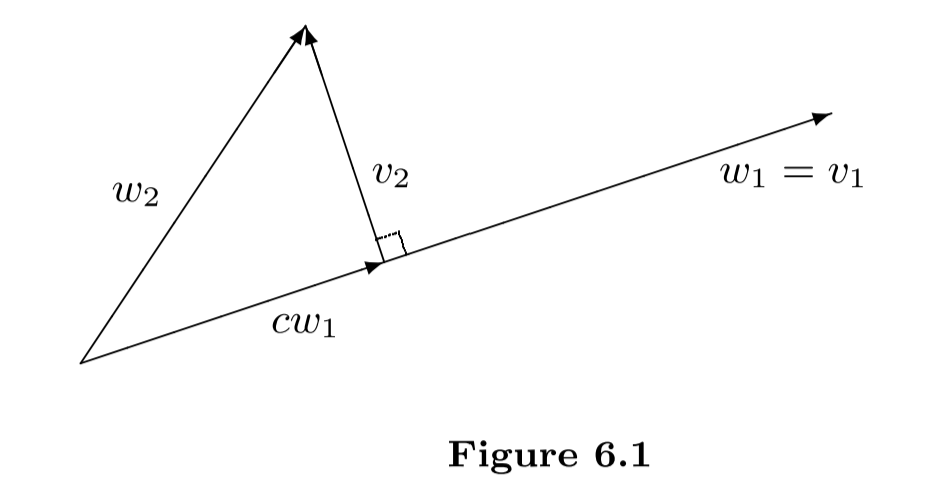
\includegraphics[width=10cm]{images/figure-6-1.png}

To find \(c\), we need only solve the following equation:
\[
    0 = \LG v_2, w_1 \RG = \LG w_2 - cw_1, w_1 \RG = \LG w_2, w_1 \RG - c \LG w_1, w_1 \RG.
\]
So
\[
    c = \frac{\LG w_1, w_2 \RG}{ \norm{w_1}^2 }
\]
Thus
\[
    v_2 = w_2 - c w_1 = w_2 - \frac{\LG w_1, w_2 \RG}{ \norm{w_1}^2 } w_1.
\]
The next theorem shows us that this process can be \emph{extended} to any \emph{finite} linearly independent subset.
\end{remark}

\begin{theorem} [Gram-Schmidt process] \label{thm 6.4}
Let \(\V\) be an inner product space and \(S = \{ w_1, w_2, ..., w_n \}\) be a \LID{} susbet of \(\V\).
Define \(S' = \{ v_1, v_2, ..., v_n \}\), where \(v_1 = w_1\) and
\[
    v_k = \RED{w_k} - \sum_{\BLUE{j = 1}}^{k - 1} \frac{\LG \RED{w_k}, \BLUE{v_j} \RG}{\norm{\BLUE{v_j}}^2} \BLUE{v_j} \quad \text{ for } 2 \le k \le n \quad \quad \MAROON{(1)}
\]
Then \(S'\) is an orthogonal set of nonzero vectors such that \(\spann(S') = \spann(S)\).
\end{theorem}

\begin{note}
The intuition is, to get \(v_k\), we need to subtract off any part of \(w_k\) ``that is \emph{not} orthogonal to the new vectors \(v_1, ..., v_{k - 1}\) we have found'', and this part is equal to the summation in \MAROON{(1)};
hence \(v_k\) will be orthogonal to all the previously found \(v_1, ..., v_k\).
\end{note}

\begin{proof}
The proof is by mathematical induction on \(n\), the \emph{number of vectors in} \(S\).
For \(k = 1, 2, ..., n\), let \(S_k = \{ w_1, w_2, ..., w_k \}\).
If \(n = 1\), then the theorem is proved by taking \(S_1' = S_1\); i.e., \(w_1 = v_1 \ne \OV\).
Assume then that the set \(S'_{k - 1} = \{ v_1, v_2, ..., v_{k-1} \}\) \emph{with the desired properties has been constructed}(i.e. \textbf{induction hypothesis}) by the repeated use of \MAROON{(1)}.
We show that the set \(S'_k = \{ v_1, v_2, ..., v_{k - 1}, v_k \}\) also has the desired properties, where \(v_k\) is obtained from \(S'_{k - 1}\) by \MAROON{(1)}.
If \(v_k = \OV\), then \MAROON{(1)} implies that \(w_k \in \spann(S'_{k - 1})\), which (by induction hypothesis) is equal to \(\spann(S_{k-1})\), which contradicts the assumption that \(S_k\) is \LID{}, hence \(v_k\) must be nonzero vector.

Now for \(1 \le i \le k- 1\), it follows from \MAROON{(1)} that
\begin{align*}
    \LG v_k, v_i \RG & = \LG w_k - \sum_{j = 1}^{k - 1} \frac{\LG w_k, v_j \RG}{\norm{v_j}^2} v_j, v_i \RG & \text{by \MAROON{(1)}} \\
        & = \LG w_k, v_i \RG - \sum_{j = 1}^{k - 1} \frac{\LG w_k, v_j \RG}{\norm{v_j}^2} \LG v_j, v_i \RG & \text{by \DEF{6.1}(a)(b)} \\
        & = \LG w_k, v_i \RG - \frac{\LG w_k, v_i \RG}{\norm{v_i}^2} \LG v_i, v_i \RG & \text{since \(S'\) is orthogonal by induction hypo} \\
        & = \LG w_k v_i \RG - \frac{\LG w_k, v_i \RG}{\norm{v_i}^2} \norm{v_i}^2 & \text{by \DEF{6.3}} \\
        & = \LG w_k v_i \RG - \LG w_k, v_i \RG = 0 & \text{of course}
\end{align*}
Hence \(v_k\) is orthogonal to \(v_1, ..., v_{k - 1}\).
With induction hypothesis that \(S'_{k - 1} = \{ v_1, ..., v_{k - 1} \}\) is orthogonal, we have that \(S'_k\) is an orthogonal set of nonzero vectors.

Now by induction hypothesis, \(\{ v_1, ..., v_{k - 1} \} = S'_{k - 1} = S_{k - 1} \subseteq S_k\).
And by \MAROON{(1)}, since each term of the right hand side is in \(S_k\), we have \(v_k\), the left hand side, in \(S_k\);
hence \(S'_{k - 1} \cup \{ v_k \} \subseteq S_k\); that is, \(S'_k \subseteq S_k\).
But (since \(S'_k\) is orthogonal and has nonzero vectors,) by \CORO{6.3.2} \(S'_k\) is \LID{}, so \(\dim(\spann(S'_k)) = k\).
But since \(S_k\) is also \LID{}, \(\dim(\spann(S_k)) = k\).
Therefore (by \THM{1.11}) \(\spann(S'_k) = \spann(S_k)\).
This closes the induction.
\end{proof}

\begin{remark} \label{remark 6.2.3}
The construction of \(\{ v_1, v_2, ..., v_n \}\) by the use of \THM{6.4} is called the \textbf{Gram-Schmidt process}.
And note that whether a set can be called orthogonal or orthonormal \textbf{depends on the inner product you choose}.
For example, the standard ordered basis for \(F^n\) is an orthonormal basis with respect to \emph{standard} inner product.
But it is not an orthonormal basis with respect to an inner product, say, \(\InnerOp' = 2 \InnerOp\), since the norm of each \(e_i\) is \(\norm{e_i}' = \sqrt{\LG e_i, e_i \RG'} = \sqrt{2 \LG e_i, e_i \RG } = \sqrt{2 \cdot 1} = \sqrt{2}\), which is not equal to \(1\).
\end{remark}

\begin{example} \label{example 6.2.4}
In \(\SET{R}^4\), let \(w_1 = (1, 0, 1, 0), w_2 = (1, 1, 1, 1)\), and \(w_3 = (0, 1, 2, 1)\).
Then \(\{ w_1, w_2, w_3 \}\) is \LID{}.
We use the Gram-Schmidt process to compute the orthogonal vectors \(v_1, v_2\), and \(v_3\), and then we normalize these vectors to obtain an orthonormal set.

Take \(v_1 = w_1 = (1, 0, 1, 0)\).
Then
\begin{align*}
    v_{\RED{2}} & = w_{\RED{2}} - \sum_{j = 1}^{\RED{2} - 1} \frac{\LG w_{\RED{2}}, v_j \RG}{\norm{v_j}^2} v_j & \text{by \THM{6.4}} \\
        & = w_2 - \frac{\LG w_2, v_1 \RG}{\norm{v_1}^2} v_1 \\
        & = (1, 1, 1, 1) - \frac{2}{2}(1, 0, 1, 0) = (0, 1, 0, 1)
\end{align*}
And
\begin{align*}
    v_{\RED{3}} & = w_{\RED{3}} - \sum_{j = 1}^{\RED{3} - 1} \frac{\LG w_{\RED{3}}, v_j \RG}{\norm{v_j}^2} v_j & \text{by \THM{6.4}} \\
        & = w_3 - \frac{\LG w_3, v_1 \RG}{\norm{v_1}^2} v_1 - \frac{\LG w_3, v_2 \RG}{\norm{v_2}^2} v_2 \\
        & = (0, 1, 2, 1) - \frac{2}{2} (1, 0, 1, 0) - \frac{2}{2} (0, 1, 0, 1) = (-1, 0, 1, 0).
\end{align*}
These vectors can be normalized to obtain the ortho\emph{normal} basis \(\{ u_1, u_2, u_3 \}\), where
\begin{align*}
    u_1 & = \frac{1}{\norm{v_1}} v_1 = \frac{1}{\sqrt{2}}(1, 0, 1, 0), \\
    u_2 & = \frac{1}{\norm{v_2}} v_2 = \frac{1}{\sqrt{2}}(0, 1, 0, 1), \\
    u_3 & = \frac{1}{\norm{v_3}} v_3 = \frac{1}{\sqrt{2}}(-1, 0, 1, 0).
\end{align*}
\end{example}

\begin{example} \label{example 6.2.5}
Let \(\V = \POLYRINF\) with the inner product
\[
    \LG f(x), g(x) \RG = \int_{-1}^{1} f(t)g(t) dt,
\]
and consider the subspace \(\POLYRR\) with the \emph{standard} ordered basis \(\beta = \{ w_1, w_2, w_3 \} = \{ 1, x, x^2 \}\).
(Note that, the point is, \(\beta\) may not be an \emph{orthogonal} basis with respect to \emph{this} inner product.)
We use the Gram Schmidt process to replace \(\beta\) by an orthogonal basis \(\{v_1, v_2, v_3 \}\) for \(\POLYRR\), \emph{with respect to} this inner product, and then use this orthogonal basis to obtain an orthonormal basis for \(\POLYRR\).

So by the process, take \(v_1 = 1\).
Then \(\norm{v_1}^2 = \LG 1, 1 \RG = \int_{-1}^1 1 \cdot 1 dt = 2\), and \(\LG x, v_1 \RG = \int_{-1}^1 t \cdot 1 dt = 0\).
Thus
\begin{align*}
    v_2 & = x - \frac{\LG x, v_1 \RG}{\norm{v_1}^2} & \text{by \THM{6.4}} \\
        & = x - \frac{0}{2} = x.
\end{align*}
Furthermore,
\[
    \LG x^2, v_1 \RG = \int_{-1}^1 t^2 \cdot 1 dt = \frac{2}{3} \quad \text{ and } \quad \LG x^2, v_2 \RG = \int_{-1}^1 t^2 \cdot t dt = 0.
\]
Therefore
\begin{align*}
    v_3 & = x^2 - \frac{\LG x^2, v_1 \RG}{\norm{v_1}^2} v_1 - \frac{\LG x^2, v_2 \RG}{\norm{v_2}^2} v_2 & \text{by \THM{6.4}} \\
        & = x^2 - \frac{1}{3} \cdot 1 - 0 \cdot x \\
        & = x^2 - \frac{1}{3}.
\end{align*}
We conclude that \(\{ 1, x, x^2 - \frac{1}{3} \}\) is an orthogonal basis for \(\POLYRR\) with respect to this inner product.

To obtain an ortho\emph{normal} basis, we normalize \(v_1, v_2\), and \(v_3\) to obtain
\begin{align*}
    u_1 & = \frac{1}{\sqrt{\int_{-1}^1 1^2 dt}} \cdot 1 = \frac{1}{\sqrt{2}}, \\
    u_2 & = \frac{1}{\sqrt{\int_{-1}^1 t^2 dt}} \cdot x = \sqrt{\frac{3}{2}} x, \\
    u_3 & = \frac{1}{\norm{v_3}} \cdot v_3 = \sqrt{\frac{5}{8}}(3x^2 - 1).
\end{align*}
Thus \(\{ u_1, u_2, u_3 \}\) is the desired orthonormal basis for \(\POLYRR\).
\end{example}

\begin{remark} \label{remark 6.2.4}
Continuing to apply the Gram-Schmidt orthogonalization process to the basis \(\{ 1, x, x^2, ... \}\) for \(\POLYRINF\), we obtain an ortho\emph{\textbf{\RED{gonal}}} basis \(\{ v_1, v_2, v_3, ... \}\).
Note that we do \emph{not} normalize them, so in particular, from \EXAMPLE{6.2.5},
\[
    \{ v_1, v_2, v_3 \} = \left\{ 1, x, x^2 - \frac{1}{3} \right\}.
\]
For each \(n\), the polynomial
\[
    \frac{1}{v_k(1)} v_k
\]
is called the \(k\)th \textbf{\href{https://www.wikiwand.com/en/Legendre_polynomials\#/Orthogonality_and_completeness}{Legendre polynomial}}.

(I don't know why we also need to multiply this additional scalar \(\frac{1}{v_k(1)}\).
In particular, why it must be true that \(v_k(1) \ne 0\) for all positive integer \(k\)?)

Then first three Legendre polynomials are
\begin{align*}
    \frac{1}{v_1(1)} v_1 & = \frac{1}{1} 1 = 1 \\
    \frac{1}{v_2(1)} v_2 & = \frac{1}{1} x = x \\
    \frac{1}{v_3(1)} v_3 & = \frac{1}{1 - \frac{1}{3}} \left( x^2 - \frac{1}{3} \right) = \frac{1}{2}(3x^2 - 1).
\end{align*}
The set of Legendre polynomials is also an orthogonal basis for \(\POLYRINF\).
\end{remark}

The following result gives us a simple method of representing a vector as a linear combination of the vectors in an ortho\emph{normal} basis.

\begin{theorem} \label{thm 6.5}
Let \(\V\) be a nonzero \emph{finite}-dimensional inner product space.
Then \(\V\) \textbf{has} an orthonormal basis \(\beta\).
Furthermore. if \(\beta = \{ v_1, v_2, ..., v_n \}\) and \(x \in \V\), then
\[
    x = \sum_{i = 1}^n \LG x, v_i \RG v_i.
\]
\end{theorem}

\begin{note}
要證明無限維度內積空間有標準正交基底也需要選擇公里或\ Zorn's Lemma.
\end{note}

\begin{proof}
Let \(\beta_0\) be an ordered basis for \(\V\).
Apply \THM{6.4} to obtain an orthogonal \emph{set} \(\beta'\) of nonzero vectors with \(\spann(\beta') = \spann(\beta_0) = \V\).
By normalizing each vector in \(\beta'\), we obtain an orthonormal \emph{set} \(\beta\) that generates \(\V\).
By \CORO{6.3.2}, \(\beta\) is \LID{}; therefore \(\beta\) is an orthonormal \emph{basis} for \(\V\).
The remainder of the theorem follows from \CORO{6.3.1}.
\end{proof}

\begin{example} \label{example 6.2.6}
We use \THM{6.5} to represent the polynomial \(f(x) = 1 + 2x + 3x^2\) as a linear combination of the vectors in the \emph{orthonormal} basis \(\{ u_1, u_2, u_3 \}\) for \(\POLYRR\) obtained in \EXAMPLE{6.2.5}.
Observe that
\[
    \LG f(x), u_1 \RG = \int_{-1}^{1} \frac{1}{\sqrt{2}} (1+2 t+3 t^2) \cdot 1 dt = 2 \sqrt{2}
\]
\[
    \LG f(x), u_2 \RG = \int_{-1}^{1} \sqrt{\frac{3}{2}} (1+2 t+3 t^2) \cdot t dt = \frac{2 \sqrt{6}}{3}
\]
and
\[
    \LG f(x), u_3 \RG = \int_{-1}^{1} \sqrt{\frac{5}{8}} (1 + 2t + 3t^2) (3 t^2 - 1) d t = \frac{2 \sqrt{10}}{5}.
\]
So by \THM{6.5}, \(f(x) = \LG f(x), u_1 \RG u_1 + \LG f(x), u_2 \RG u_2 + \LG f(x), u_3 \RG u_3 = 2 \sqrt{2} u_1 + \frac{2 \sqrt{6}}{3} u_2 + \frac{2 \sqrt{10}}{5} u_3\).
\end{example}

\THM{6.5} gives us a simple method for computing the entries of the \textbf{matrix representation} of a linear operator \textbf{with respect to an orthonormal basis}.

\begin{corollary} \label{corollary 6.5.1}
Let \(\V\) be a \emph{finite}-dimensional inner product space with an \emph{orthonormal} basis \(\beta = \{ v_1, v_2, ..., v_n \}\).
Let \(\T\) be a linear operator on \(\V\), and let \(A = [\T]_{\beta}\).
Then for any \(i\) and \(j\), \(A_{ij} = \LG \T(v_j), v_i \RG\).
(Notice the order of \(i\) and \(j\) in the equation.)
\end{corollary}

\begin{proof}
In particular from \THM{6.5}, we have
\[
    \T(v_j) = \sum_{i = 1}^n \LG \T(v_j), v_i \RG v_i.
\]
Hence by definition of matrix representation, \(A_{ij} = \LG \T(v_j), v_i \RG\).
\end{proof}

\begin{remark} \label{remark 6.2.5}
The scalars \(\LG x, v_i \RG\) given in \THM{6.5} have been studied \emph{extensively} for special inner product spaces. 
Although the vectors \(v_1, v_2, ..., v_n\) were chosen from an orthonormal basis, we introduce a terminology associated
with orthonormal sets \(\beta\) in more general inner product spaces.
\end{remark}

\begin{definition} \label{def 6.6}
Let \(\beta\) be an orthonormal subset (possibly infinite) of an inner product space \(\V\), and let \(x \in \V\).
We define the \textbf{Fourier coefficient\RED{s}} of \(x\) relative to \(\beta\) to be the scalars \(\LG x, y \RG\), where \(y \in \beta\).
\end{definition}

\begin{remark} \label{remark 6.2.6}
In the first half of the 19th century, the French mathematician Jean Baptiste Fourier was associated with the study of the \emph{scalars} (for any integer \(n\))
\[
    \int_0^{2\pi} f(t) \sin nt dt \quad \text{ and } \quad \int_0^{2\pi} f(t) \cos nt dt
\]
or in the complex case,
\[
    c_n = \frac{1}{2\pi} f(t) e^{-\iu n t} dt.
\]
for a function \(f\).
In the context of \EXAMPLE{6.1.9}, we see that \(c_n = \LG f, f_n \RG\), where \(f_n(t) = e^{\iu nt}\); that is, \(c_n\) is the nth \emph{Fourier coefficient} for a continuous function \(f \in \textsf{H}\) relative to \(S\).
The coefficients \(c_n\) are the ``classical'' Fourier coefficients of a function, and the literature concerning their behavior is extensive.
We learn more about Fourier coefficients in the remainder of this chapter.
\end{remark}

\begin{example} \label{example 6.2.7}
Let \(S = \{ e^{\iu n t} : n \text{ is an integer} \}\).
In \EXAMPLE{6.1.9}, \(S\) was shown to be an orthonormal set in \(\textsf{H}\).
We compute the Fourier coefficients of \(f(t) = t\) relative to \(S\).
Using \emph{integration by parts}, we have, for \(n \ne 0\),
\[
    \LG f, f_n \RG = \frac{1}{2\pi} \int t \conjugatet{e^{\iu n t}} dt = \int \frac{1}{2\pi} t e^{-\iu n t} dt = \frac{-1}{\iu n}, \quad \MAROON{(1)}
\]
and, for \(n = 0\),
\[
    \LG f, f_n \RG = \LG f, e^0 \RG = \LG f, 1 \RG = \int \frac{1}{2\pi} t \cdot 1 dt = \pi. \quad \MAROON{(2)}
\]
As a result of these computations, and using \EXEC{6.2.16}, we obtain an \emph{upper bound} for the sum of a special \emph{infinite series}, \(\sum_{i = 1}^{\infty} \frac{1}{n^2}\), as follows:
(Note that since \(S\) is orthonormal, in particular \(S_k = \{ e^{\iu n t} : -k \le n \le k \}\) is orthonormal.)
\begin{align*}
    \norm{f}^2 & \ge \sum_{n = -k}^k \abs{ \LG f, f_n \RG }^2 & \text{by \EXEC{6.2.16} with aforementioned \(S_k\)} \\
        & = \sum_{n = -k}^{-1} \abs{ \LG f, f_n \RG }^2 + \abs{ \LG f, 1 \RG }^2 + \sum_{n = 1}^k \abs{f, f_n}^2 \\
        & = \sum_{n = -k}^{-1} \frac{1}{n^2} + \pi^2 + \sum_{n = 1}^k \frac{1}{n^2} & \text{by using \MAROON{(1)(2)}, but taking square} \\
        & = 2 \sum_{n = 1}^k \frac{1}{n^2} + \pi^2 & \text{of course}
\end{align*}
for every \(k\).

Now, using the fact that \(\norm{f}^2 = \frac{4}{3}\pi^2\), we obtain
\[
    \frac{4}{3}\pi^2 \ge 2 \sum_{n = 1}^k \frac{1}{n^2} + \pi^2,
\]
or
\[
    \frac{\pi^2}{6} \ge \sum_{n = 1}^k \frac{1}{n^2}.
\]
Because this inequality holds \emph{for all} \(k\), we may let \(k \to \infty\) to obtain
\[
    \frac{\pi^2}{6} \ge \sum_{n = 1}^{\infty} \frac{1}{n^2}.
\]
Additional results may be produced by replacing \(f\) by other functions.
\end{example}

\begin{note}
(My professor said) The inequality we have shown is in fact an equality, but the proof need some technique in Analysis courses.
\end{note}

We are now ready to proceed with the concept of an \emph{orthogonal complement}.

\begin{definition} \label{def 6.7}
Let \(S\) be a nonempty subset of an inner product space \(\V\).
We define \(S^{\perp}\) (read ``\(S\) perp'') to be the set of all vectors in \(\V\) that are \emph{orthogonal} to every vector in \(S\);
that is, \(S^{\perp} = \{ x \in \V: \LG x, y \RG = 0 \text{ for all } y \in S\}\).
The set \(S^{\perp}\) is called the \textbf{orthogonal complement} of \(S\).

It is easily seen that \(S^{\perp}\) is a subspace of \(\V\) for any subset \(S\) of \(\V\). (See \EXEC{6.2.1}(c).)

And in particular, if \(S\) itself is also a subspace, then \(S \cap S^{\perp} = \{ \OV \}\).
(Otherwise if \(v \in S\) and \(v \in S^{\perp}\) where \(v \ne \OV\), the we have \(\LG \BLUE{v}, \RED{v} \RG = 0\) where \(\BLUE{v} \in S^{\perp}\) and \(\RED{v} \in S\), but this contradicts \DEF{6.1}(d).)
\end{definition}

\begin{example} \label{example 6.2.8}
The reader should verify that \(\{ \OV \}^{\perp} = \V\) and \(\V^{\perp} = \{ \OV \}\) for any inner product space \(\V\).
\end{example}

\begin{example} \label{example 6.2.9}
If \(\V = \SET{R}^3\) and \(S = \{ e_3 \}\), then \(S^{\perp}\) equals the \(xy\)-plane (see \EXEC{6.2.5}).
\end{example}

\EXEC{6.2.18} provides an interesting example of an orthogonal complement in an \emph{infinite}-dimensional inner product space. 
\begin{remark} \label{remark 6.2.7}
Consider the problem in \(\SET{R}^3\) of finding the \emph{distance} from a point \(P\) to a plane \(\W\).
(See Figure 6.2.)

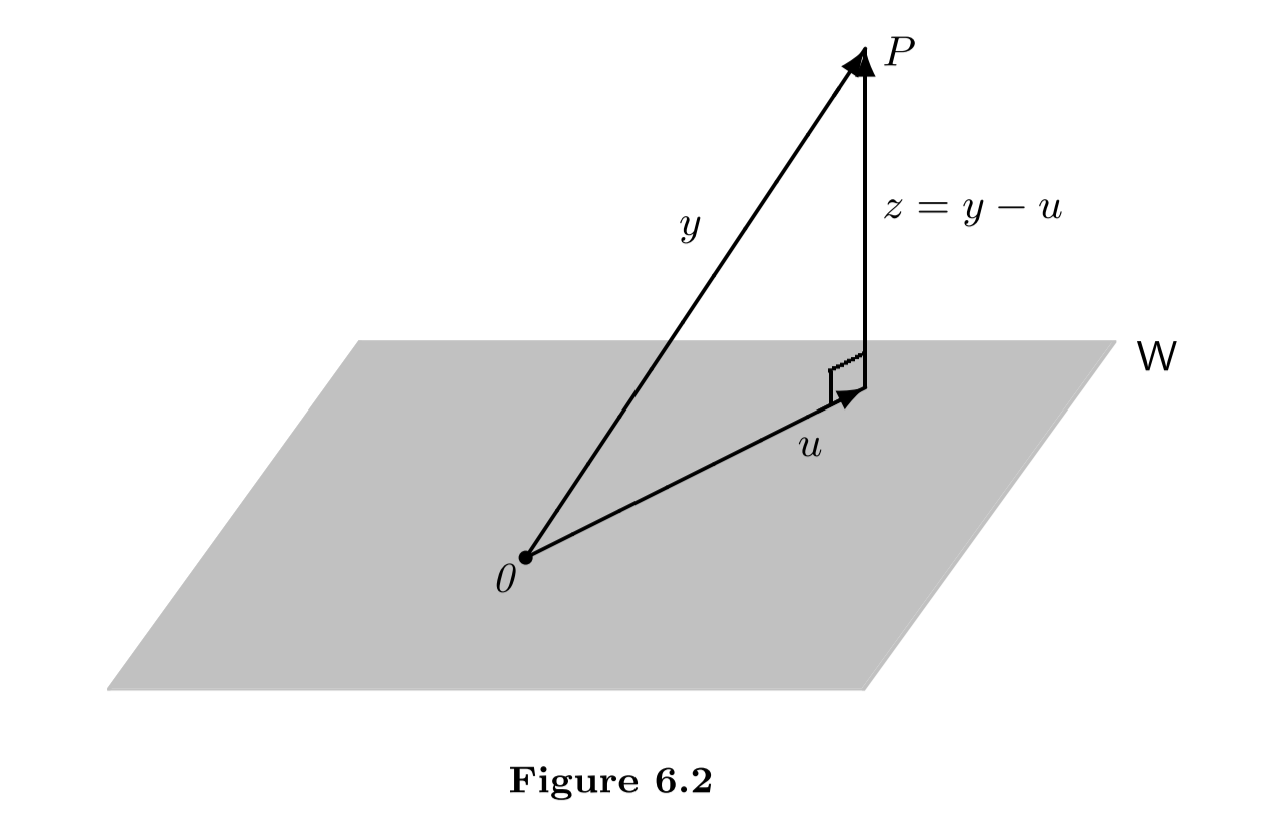
\includegraphics[width=12cm]{images/figure-6-2.png}

(This is high school algebra, but) Problems of this type arise in many settings.
If we let \(y\) be the vector determined by \(0\) and \(P\).
We may restate the problem as follows:
Determine the vector \(u\) in \(\W\) that is ``\textbf{closest}'' to \(y\).
The desired distance is clearly given by \(\norm{y - u}\).
\emph{Notice} from the figure that the vector \(z = y - u\) is \emph{orthogonal} to \textbf{every vector} in \(\W\), and so \(z \in \W^{\perp}\).

The next result presents a practical method of finding \(u\) in the case that \(\W\) is a \emph{finite}-dimensional \emph{subspace} of an inner product space.
\end{remark}

\begin{theorem} \label{thm 6.6}
Let \(\W\) be a \emph{finite}-dimensional subspace of an inner product space \(\V\), and let \(y \in \V\).
Then \emph{there exist} \textbf{unique} vector \(u \in \W\) and \textbf{unique} vector \(z \in \W^{\perp}\), such that \(y = u + z\).
Furthermore, if \(\{ v_1, v_2, ..., v_k \}\) is an orthonormal basis \textbf{for \(\W\)}, then
\[
    u = \sum_{i = 1}^k \LG y, v_i \RG v_i.
\]
\end{theorem}

\begin{note}
\THM{6.6} 就是最廣義的看法:
給定一個子空間 \(\W\),然後給定一個向量\ \(y \in \V\),這個向量\ \(y\) 可以拆成\textbf{唯一的}表示法\ \(u + z\),使得\ \(u \in \W\),\(z \in \W^{\perp}\)。
另外\ \(u\) 就是\ \textbf{\(y\) 在\ \(\W\) 的「投影」},並且可用\ \(\W\) 的\ orthonormal basis 來表示,係數就是\ \(y\) 對每個\ basis vector 的投影量。
如果是\ \(\SET{R}^3\) 的例子就會是\ Figure 6.2。
\end{note}

\begin{proof}
Let \(\{ v_1, v_2, ..., v_k \}\) be an orthonormal basis for \(\W\), let \(u\) be as defined in the preceding equation, and let \(z = y - u\). Clearly \(u \in \W\) and \(y = u + z\).

To show that \(z \in \W^{\perp}\), it suffices to show, by \EXEC{6.2.7}, that \(z\) is orthogonal to each \(v_j\) for \(1 \le j \le k\).
So for any \(j\), we have
\begin{align*}
    \LG z, v_j \RG & = \LG y - u, v_j \RG = \LG y - \sum_{i = 1}^k \LG y, v_i \RG v_i, v_j \RG & \text{of course} \\
        & = \LG y, v_j \RG - \sum_{i = 1}^k \LG y, v_i \RG \LG v_i, v_j \RG & \text{by \DEF{6.1}(a)(b)} \\
        & = \LG y, v_j \RG - \LG y, v_{\RED{j}} \RG \LG v_{\RED{j}}, v_j \RG & \text{since \(v_i\)'s are in particular orthogonal} \\
        & = \LG y, v_j \RG - \LG y, v_{j} \RG \norm{v_j}^2 & \text{by \DEF{6.3}} \\
        & = \LG y, v_j \RG - \LG y, v_{j} \RG \cdot 1 = \LG y, v_j \RG - \LG y, v_{j} \RG & \text{since \(v_i\)'s are ortho\emph{normal}} \\
        & = 0.
\end{align*}
Hence \(z \in \W^{\perp}\), hence the existence part that \(y = u + z\) where \(u \in \W\) and \(z \in \W^{\perp}\) is showed.

Now for the uniqueness part, suppose that \(y = u + z = u' + z'\), where \(u' \in \W\) and \(z' \in \W^{\perp}\).
Then in particular by arranging equation, \(u - u' = z'- z\); but \(u - u' \in \W\) and \(z' - z \in \W^{\perp}\), so the equation implies both \(u - u', z' - z \in \W \cap \W^{\perp}\).
But in \DEF{6.7} we have shown \(\W \cap \W^{\perp} = \{ \OV \}\), hence \(u - u' = z' - z = \OV\), hence \(u = u'\) and \(z = z'\), showing the uniqueness.
\end{proof}

\begin{corollary} \label{corollary 6.6.1}
In the notation of \THM{6.6}, the vector \(u\) is the unique vector in \(\W\) that is ``closest'' to \(y\);
that is, for any \(x \in \W\), \(\norm{y - x} \ge \norm{y - u}\), and this inequality is an equality if and only if \(x = u\).
\end{corollary}

\begin{proof}
As in \THM{6.6}, we have that \(y = u + z\), where \(z \in \W^{\perp}\).
Let \(x \in \W\).
Then \(u - x \in \W\), hence is orthogonal to \(z\). \MAROON{(1)}

So by \EXEC{6.1.10}, we have
\begin{align*}
    \norm{y - x}^2 & = \norm{(u + z) - x}^2 = \norm{(u - x) + z^2} & \text{tricky but of course} \\
        & = \norm{u - x}^2 + \norm{z}^2 & \text{by \MAROON{(1)} and \EXEC{6.1.10}} \\
        & \ge \norm{z}^2 & \text{by \THM{6.2}(b), \(\norm{u - x}^2 \ge 0\)} \\
        & = \norm{y - u}^2, & \text{of course}
\end{align*}
which implies \(\norm{y - x} \ge \norm{y - u}\).

Now suppose that \(\norm{y - x} = \norm{y - u}\).
Then the inequality above becomes an equality, and therefore \(\norm{u - x}^2 + \norm{z}^2 = \norm{z}^2\).
It follows that \(\norm{u - x} = 0\), and hence (by \THM{6.2}(a)) \(x = u\).

For the converse, if \(x = u\), then of course \(y - x = y - u\) hence of course \(\norm{y - x} = \norm{y - u}\).
\end{proof}

\begin{additional definition} \label{adef 6.3}
The vector \(u\) in the corollary is called the \textbf{orthogonal projection} of \(y\) on \(\W\).
We will see the importance of orthogonal projections of vectors in the application to \emph{least squares} in \SEC{6.3}.
\end{additional definition}

\begin{example} \label{example 6.2.10}
Let \(\V = \POLYRRR\) with the inner product
\[
    \LG f(x),g(x) \RG = \int_{-1}^{1} f(t)g(t) dt
\]
for all \(f(x), g(x) \in \V\).
We compute the orthogonal projection of \(f(x) = x^3\) on \(\POLYRR\).
Let it be \(f_1(x)\).

By \EXAMPLE{6.2.5},
\[
    \{ u_1, u_2, u_3 \} = \left\{ \frac{1}{\sqrt{2}}, \sqrt{\frac{3}{2}} x, \sqrt{\frac{5}{8}}(3x^2 - 1) \right\}
\]
is an orthonormal basis for \(\POLYRR\).
By \THM{6.6}, we need to compute \(\LG f(x), u_1 \RG, \LG f(x), u_2 \RG\) and \(\LG f(x), u_3 \RG\).
So we have
\[
    \LG f(x), u_1 \RG = \int_{-1}^{1} t^3 \frac{1}{\sqrt{2}} dt = 0,
    \quad \LG f(x), u_2 \RG = \int_{-1}^{1} t^3 \sqrt{\frac{3}{2}} t dt = \frac{\sqrt{6}}{5}
\]
and
\[
    \LG f(x), u_3 \RG = \int_{-1}^{1} t^{3} \sqrt{\frac{5}{8}} (3 t^2 - 1) dt = 0
\]
Hence
\begin{align*}
    f_{1}(x) & = \LG f(x), u_1 \RG u_1 + \LG f(x), u_2 \RG u_2 + \LG f(x), u_3 \RG u_3 & \text{by \THM{6.6}} \\
        & = 0 u_1 + \frac{\sqrt{6}}{5} u_2 + 0 u_3 \\
        & = \frac{\sqrt{6}}{5} \cdot \sqrt{\frac{3}{2}}x = \frac{3}{5} x
\end{align*}
\end{example}

\begin{remark} \label{remark 6.2.8}
It was shown in \CORO{1.10.2}(corollary to the replacement theorem) that any \LID{} set in a \emph{finite}-dimensional vector space can be \emph{extended} to a basis.
The next theorem provides an interesting analog for an orthonormal subset of a \emph{finite}-dimensional inner product space.
\end{remark}

\begin{theorem} \label{thm 6.7}
Suppose that \(S = \{ v_1, v_2, ..., v_k \}\) is an orthonormal set in an \(n\)-dimensional inner product space \(\V\).
Then
\begin{enumerate}
\item \(S\) can be extended to an \textbf{orthonormal} basis \(\{ v_1, v_2, ..., v_k, v_{k+1}, ..., v_n \}\) for \(\V\).
\item If \(\W = \spann(S)\), then \(S_1 = \{v_{k+1}, v_{k+2}, ..., v_n \}\) is an orthonormal basis for \(\W^{\perp}\) (using the preceding notation).
\item If \(\W\) is any \emph{subspace} of \(\V\), then \(\dim(\V) = \dim(\W) + \dim(\W^{\perp})\).
\end{enumerate}
\end{theorem}

\begin{proof} \ 

\begin{enumerate}
\item By \CORO{1.10.2}, \(S\) can be extended to an \emph{ordered basis} \(S' = \{ v_1, v_2, ..., v_{k}, w_{k+1}, ..., w_n \}\) for \(\V\).
Now apply the Gram-Schmidt process to \(S'\).
By \EXEC{6.2.8}, the first \(k\) vectors resulting from this process \textbf{are still the vectors in \(S\)} , and this new set spans \(\V\).
Normalizing the last \(n - k\) vectors of this set produces an orthonormal set that spans \(\V\).
The result now follows.

\item Because \(S_1\) is a subset of a (orthonormal) basis, it is \LID{}.
And for every vector in \(S_1\), it is orthogonal to every vector in \(S\), hence is orthogonal to every vector in \(\spann(S) = \W\), so by \DEF{6.7} it is in \(\W^{\perp}\), hence \(S_1 \subseteq \W^{\perp}\).

Now we show that it spans \(\W^{\perp}\).
Note that \(\spann(S_1) \subseteq \W^{\perp}\) is automatically true.
And for any \(x \in \V\), since \(\{ v_1, v_2, ..., v_n \}\) is an orthonormal basis, (by \THM{6.5}) we have
\[
    x = \sum_{i = 1}^n \LG x, v_i \RG v_i.
\]
Now if \(x\) is also in \(\W^{\perp}\), then \(\LG x, v_i \RG = 0\) for \(1 \le i \le k\).
Therefore
\[
    x = \sum_{i = k + 1}^n \LG x, v_i \RG v_i \in \spann(S_1).
\]
Hence \(\W^{\perp} \subseteq \spann(S_1)\).
Hence \(\W^{\perp} = \spann(S_1)\).
So \(S_1\) generates \(\W^{\perp}\) and is \LID{}, hence is a basis for \(\W^{\perp}\).

\item Let \(\W\) be a subspace of \(\V\).
It is a \emph{finite}-dimensional inner product space because \(\V\) is, and so it has an orthonormal basis \(\{ u_1, u_2, ..., u_k \}\).
By (a) and (b). we have
\begin{align*}
    & \dim(\V) \\
    & = n = k + (n - k) & \text{of course} \\
    & = \dim(\W) + (n - k) & \text{\(\{ u_1, ..., u_k \}\) is a basis for \(\W\)} \\
    & = \dim(\W) + \dim(\W^{\perp}) & \text{by (a)(b), the extended \(\{ u_{k + 1}, ..., u_{n} \}\) is a basis for \(\W^{\perp}\)}
\end{align*}
\end{enumerate}
\end{proof}

\begin{example} \label{example 6.2.11}
Let \(\W = \spann(\{ e_1, e_2 \})\) in \(F^3\).
Then \(x = (a, b, c) \in \W^{\perp}\) if and only if \(0 = \LG x, e_1 \RG = a\) and \(0 = \LG x , e_2 \RG = b\).
So \(x = (0, 0, c)\), and therefore \(\W^{\perp} = \spann(\{ e_3 \})\).
One can deduce the same result by noting that \(e_3 \in \W^{\perp}\) and, from \THM{6.7}(c), that \(\dim(\W^{\perp}) = \dim(V) - \dim(W) = 3 - 2 = 1\).
\end{example}

\exercisesection

\begin{exercise} \label{exercise 6.2.1}
Label the following statements as true or false.
\begin{enumerate}
\item The Gram-Schmidt orthogonalization process produces an orthonormal set from an arbitrary \emph{\LID{}} set.
\item Every nonzero finite-dimensional inner product space has an orthonormal basis.
\item The orthogonal complement of any set is a subspace.
\item If \(\{ v_1, v_2, ..., v_n \}\) is a basis for an inner product space \(\V\), then for any \(x \in \V\) the scalars \(\LG x, v_i \RG\) are the Fourier coefficients of \(x\).
\item An orthonormal basis must be an ordered basis.
\item Every orthogonal set is linearly independent.
\item Every orthonormal set is linearly independent.
\end{enumerate}
process 那提很尷尬;gen 出來的嚴格來說是 orthogonal,但是把 process 多一步做 normalize 也可以吧
Fourier coefficients 那個,basis 要 orthonormal ==
\end{exercise}

\begin{proof}
\end{proof}

\begin{exercise} \label{exercise 6.2.2}
In each part, apply the Gram-Schmidt process to the given subset \(S\) of the inner product space \(\V\) to obtain an orthogonal basis for \(\spann(S)\).
Then normalize the vectors in this basis to obtain an orthonormal basis \(\beta\) for \(\spann(S)\), and compute the Fourier coefficients of the given vector relative to \(\beta\).
Finally, use \THM{6.5} to verify your result.

\begin{enumerate}
\item \(\V = \SET{R}^3, S = \{ (1, 0, 1), (0, 1, 1), (1, 3, 3) \}\), and \(x = (1, 1, 2)\)
\item \(\V = \SET{R}^3, S = \{ (1, 1, 1), (0, 1, 1), (0, 0, 1) \}\), and \(x = (1, 0, 1)\)
\item \(\V = \POLYRR\) with the inner product \(\LG f(x), g(x) \RG = \int_0^1 f(t) g(t) dt, S = \{1, x, x^2 \}\), and \(h(x) = 1 + x\)
\item \(\V = \spann(S)\), where \(S = \{(1, \iu, 0), (1 - \iu, 2, 4\iu) \}\), and \(x = (3 + \iu, 4\iu, -4)\)
\item \(\V = \SET{R}^4, S = \{ (2, -1, -2, 4), (-2, 1, -5, 5), (-1, 3, 7, 11) \}\), and \(x = (-11, 8, -4, 18)\)
\item \(\V = \SET{R}^4, S = \{ (1, -2, -1, 3), (3, 6, 3, -1), (1, 4, 2, 8) \}\), and \(x = (-1, 2, 1, 1)\)
\item \(\V = M_{2 \X 2}(\SET{R}),
    S = \left\{
        \begin{pmatrix}3 & 5 \\ -1 & 1\end{pmatrix},
        \begin{pmatrix}-1 & 9 \\ 5 & -1\end{pmatrix},
        \begin{pmatrix}7 & -17 \\ 2 & -6\end{pmatrix}\right
    \}\),
    and \(A = \begin{pmatrix}-1 & 27 \\ -4 & 8\end{pmatrix}\)
\item \(\V = M_{2 \X 2}(\SET{R}),
    S = \left\{
        \begin{pmatrix}2 & 2 \\ 2 & 1\end{pmatrix},
        \begin{pmatrix}11 & 4 \\ 2 & 5\end{pmatrix},
        \begin{pmatrix}4 & -12 \\ 3 & -16\end{pmatrix}
    \right\}\),
    and \(A = \begin{pmatrix}8 & 6 \\ 25 & -13\end{pmatrix}\)
\item \(\V = \spann(S)\) with the inner product \(\LG f, g \RG = \int_0^{\pi} f(t)g(t) dt, S = \{\sin t, \cos t, 1, t\}\), and \(h(t) = 2t + 1\)
\item \(\V = \SET{C}^4,
    S = \{ (1, i, 2 - \iu, -1), (2 + 3\iu, 3\iu, 1 - \iu, 2\iu), (-1 + 7\iu, 6 + 10\iu, 11 - 4\iu, 3 + 4\iu)\}\),
    and \(x = (-2 + 7\iu, 6 + 9\iu, 9 - 3\iu, 4 + 4\iu)\)
\item \(\V = \SET{C}^4, S = \{(-4, 3 - 2\iu, \iu, 1 - 4\iu), (-1 - 5\iu, 5 - 4\iu, -3 + 5\iu, 7 - 2\iu), (-27 - \iu, -7 - 6\iu, -15 + 25\iu, -7 - 6\iu)\}\), and \(x = (-13 - 7\iu, -12 + 3\iu, -39 - 11\iu, -26 + 5\iu)\)
\item \(\V = M_{2 \X 2}(\SET{C})\),
\[
    S = \left\{
        \begin{pmatrix} 1 - \iu & -2 - 3\iu \\ 2 + 2\iu & 4 + \iu \end{pmatrix},
        \begin{pmatrix} 8\iu & 4 \\ -3 - 3\iu & -4 + 4\iu \end{pmatrix},
        \begin{pmatrix} -25 - 38\iu & -2 - 13\iu \\ 12 - 78\iu & -7 + 24\iu \end{pmatrix}
    \right\},
\]
and \(A=\begin{pmatrix} -2 + 8\iu & -13 + \iu \\ 10 - 10\iu & 9 - 9\iu \end{pmatrix}\)
\item \(\V = M_{2 \X 2}(\SET{C})\),
\[
    S = \left\{
        \begin{pmatrix} -1 + \iu & -\iu \\ 2 - \iu & 1 + 3\iu\end{pmatrix},
        \begin{pmatrix} -1 - 7\iu & -9 - 8\iu \\ 1 + 10\iu & -6 - 2\iu\end{pmatrix},
        \begin{pmatrix} -11 - 132\iu & -34 -31\iu \\ 7 - 126\iu & -71 - 5\iu \end{pmatrix}
    \right\},
\]
and \(A=\begin{pmatrix} -7 + 5\iu & 3 + 18\iu \\ 9 - 6\iu & -3 + 7\iu \end{pmatrix}\)
\end{enumerate}
\end{exercise}

\begin{proof}
手寫吧... 跳過
\end{proof}

\begin{exercise} \label{exercise 6.2.3}
In \(\SET{R}^2\), let
\[
    \beta = \left\{
        \left( \frac{1}{\sqrt{2}}, \frac{1}{\sqrt{2}} \right), \left( \frac{1}{\sqrt{2}}, \frac{-1}{\sqrt{2}} \right)
    \right\}
\]
Find the Fourier coefficients of \((3, 4)\) relative to \(\beta\).
\end{exercise}

\begin{proof}
\end{proof}

\begin{exercise} \label{exercise 6.2.4}
Let \(S = \{ (1, 0, \iu), (1, 2, 1) \}\) in \(\SET{C}^3\). Compute \(S^{\perp}\).
\end{exercise}

\begin{proof}
\end{proof}

\begin{exercise} \label{exercise 6.2.5}
Let \(S_0 = \{ x_0 \}\), where \(x_0\) is a nonzero vector in \(\SET{R}^3\).
Describe \(S_0^{\perp}\) geometrically.
Now suppose that \(S = \{ x_1, x_2 \}\) is a \LID{} subset of \(\SET{R}^3\).
Describe \(S^{\perp}\) geometrically.
\end{exercise}

\begin{proof}
\end{proof}

\begin{exercise} \label{exercise 6.2.6}
Let \(\V\) be an inner product space, and let \(\W\) be a \emph{finite}-dimensional subspace of \(\V\).
If \(x \notin \W\), prove that there \emph{exists} \(y \in \V\) such that \(y \in W^{\perp}\), but \(\LG x, y \RG \ne 0\).
Hint: Use \THM{6.6}.
\end{exercise}

\begin{proof}
\end{proof}

\begin{exercise} \label{exercise 6.2.7}
Let \(\beta\) be a basis for a subspace \(\W\) of an inner product space \(\V\), and let \(z \in \V\).
Prove that \(z \in \W^{\perp}\) if and only if \(\LG z, v \RG = 0\) for every \(v \in \beta\).
\end{exercise}

\begin{note}
又一題,只要檢查 basis 行為就可決定整體行為的。
\end{note}

\begin{proof}
\end{proof}

\begin{exercise} \label{exercise 6.2.8}
Prove that if \(\{ w_1, w_2, ..., w_n \}\) is an \emph{orthogonal} set of nonzero vectors, then the vectors \(v_1, v_2, ..., v_n\) derived from the Gram-Schmidt process \emph{satisfy} \(v_i = w_i\) for \(i = 1, 2, ..., n\).
Hint: Use mathematical induction.
\end{exercise}

\begin{proof}
\end{proof}

\begin{exercise} \label{exercise 6.2.9}
Let \(\W = \spann(\{ ( \iu, 0, 1) \})\) in \(\SET{C}^3\).
Find orthonormal bases for \(\W\) and \(\W^{\perp}\).
\end{exercise}

\begin{proof}
\end{proof}

\begin{exercise} \label{exercise 6.2.10}
Let \(\W\) be a \emph{finite}-dimensional subspace of an inner product space \(\V\).
Prove that \(\V = \W \oplus \W^{\perp}\).
Using the \ADEF{2.2}, prove that there exists a projection \(\T\) on \(\W\) along \(\W^{\perp}\) that satisfies \(\NULLT = \W^{\perp}\).
In addition, prove that \(\norm{\T(x)} \le \norm{x}\) for all \(x \in \V\).
Hint: Use \THM{6.6} and \EXEC{6.1.10}.
\end{exercise}

\begin{proof}
這感覺用 1.6 3x 題 dim v = dim w + dim w perp 可以吧?
\end{proof}

\begin{exercise} \label{exercise 6.2.11}
Let \(A\) be an \(n \X n\) matrix with \emph{complex} entries.
Prove that \(A A^* = I\) if and only if the \emph{rows} of \(A\) form an \emph{orthonormal} basis for \(\SET{C}^n\).
\end{exercise}

\begin{proof}
\end{proof}

\begin{exercise} \label{exercise 6.2.12}
Prove that for any matrix \(A \in M_{m \X n}(F)\), \((\RANGE(\LMTRAN_{A^*}))^{\perp} = \NULL(\LMTRAN_A)\).
\end{exercise}

\begin{note}
幹,怕
A 的零空間會跟 A 的共軛轉置矩陣的 range 的正交補集一樣
\end{note}

\begin{proof}
\end{proof}

\begin{exercise} \label{exercise 6.2.13}
Let \(\V\) be an inner product space, \(S\) and \(S_0\) be \emph{subsets} of \(\V\), and \(\W\) be a finite-dimensional \emph{subspace} of \(\V\).
Prove the following results.
\begin{enumerate}
\item \(S_0 \subseteq S\) implies that \(S^{\perp} \subseteq S_0^{\perp}\).
\item \(S \subseteq (S^{\perp})^{\perp}\); so \(\spann(S) \subseteq (S^{\perp})^{\perp}\).
\item \(\W = (\W^{\perp})^{\perp}\). Hint: Use \EXEC{6.2.6}.
\item \(\V = \W \oplus \W^{\perp}\). (See the exercises of \SEC{1.3}.)
\end{enumerate}
\end{exercise}

\begin{proof}
(d) 在銃殺小? 第十題不就有了?
\end{proof}

\begin{exercise} \label{exercise 6.2.14}
Let \(\W_1\) and \(\W_2\) be subspaces of a \emph{finite}-dimensional inner product space.
Prove that \((\W_1 + \W_2)^{\perp} = \W_1^{\perp} \cap \W_2^{\perp}\) and \((\W_1 \cap \W_2)^{\perp} = \W_1^{\perp} + \W_2^{\perp}\).
Hint for the second equation: Apply \EXEC{6.2.13}(c) to the first equation.
\end{exercise}

\begin{proof}
\end{proof}

\begin{exercise} \label{exercise 6.2.15}
Let \(\V\) be a \emph{finite}-dimensional inner product space over \(F\).
\begin{enumerate}
\item \emph{Parseval's Identity}.
Let \(\{ v_1, v_2, ..., v_n \}\) be an orthonormal basis for \(\V\).
For any \(x, y \in \V\) prove that
\[
    \LG x, y \RG = \sum_{i = 1}^n \LG x, v_i \RG \conjugatet{\LG y, v_i \RG}.
\]
\item Use (a) to prove that if \(\beta\) is an orthonormal basis for \(\V\) with inner product \(\InnerOp\), then for any \(x, y \in \V\)
\[
    \LG \phi_{\beta}(x), \phi_{\beta}(y) \RG' = \LG [x]_{\beta}, [y]_{\beta} \RG' = \LG x, y \RG,
\]
where \(\InnerOp'\) is the \emph{standard} inner product on \(F^n\).
\end{enumerate}
\end{exercise}

\begin{proof}
\end{proof}

\begin{exercise} \label{exercise 6.2.16} \ 

\begin{enumerate}
\item \emph{Bessel's Inequality}.
Let \(\V\) be an inner product space, and let \(S = \{ v_1, v_2, ..., v_n \}\) be an orthonormal subset of \(\V\).
Prove that for any \(x \in \V\) we have
\[
    \norm{x}^2 \ge \sum_{i = 1}^n \abs{\LG x, v_i \RG}^2.
\]
Hint: Apply \THM{6.6} to \(x \in \V\) and \(\W = \spann(S)\).
Then use \EXEC{6.1.10}.
\item In the context of (a), prove that Bessel's inequality is an equality if and only if \(x \in \spann(S)\).
\end{enumerate}
\end{exercise}

\begin{proof}
\end{proof}

\begin{exercise} \label{exercise 6.2.17}
Let \(\T\) be a linear operator on an inner product space \(\V\).
If \(\LG \T(x), y \RG = 0\) for all \(x, y \in \V\), prove that \(\T = \TZERO\).
In fact, prove this result if the equality holds for all \(x\) and \(y\) in some \emph{basis} for \(\V\).
\end{exercise}

\begin{proof}
\end{proof}

\begin{exercise} \label{exercise 6.2.18}
Let \(\V = \CONT([-1, 1])\).
Suppose that \(\W_e\) and \(\W_o\) denote the subspaces of \(\V\) consisting of the \emph{even} and \emph{odd} functions, respectively.
Prove that \(\W_e^{\perp} = W_o\), where the inner product on \(\V\) is defined by
\[
    \LG f, g \RG = \int_{-1}^1 f(t) g(t) dt.
\]
\end{exercise}

\begin{proof}
\end{proof}

\begin{exercise} \label{exercise 6.2.19}
In each of the following parts, find the orthogonal projection of the given vector on the given subspace \(\W\) of the inner product space \(\V\).
\begin{enumerate}
\item \(\V = \SET{R}^2, u = (2, 6)\), and \(\W = \{ (x, y): y = 4x \}\).
\item \(\V = \SET{R}^3, u = (2, 1, 3)\), and \(\W = \{ (x, y, z): x + 3y - 2z = 0 \}\).
\item \(\V = \POLYRINF\) with the inner product \(\LG f(x), g(x) \RG = \int_0^1 f(t) g(t) dt, h(x) = 4 + 3x - 2x^2\), and \(\W = \POLYR\).
\end{enumerate}
\end{exercise}

\begin{proof}
\end{proof}

\begin{exercise} \label{exercise 6.2.20}
In each part of \EXEC{6.2.19}, find the distance from the given vector to the subspace \(\W\).
\end{exercise}

\begin{proof}
\end{proof}

\begin{exercise} \label{exercise 6.2.21}
Let \(\V = \CONT([-1, 1])\) with the inner product \(\LG f,g \RG = \int_{-1}^1 f(t)g(t) dt\), and let \(\W\) be the subspace \(\POLYRR\), viewed as a space \emph{of functions}.
(See the difference between polynomial and polynomial \emph{functions} in \RMK{e.7}.)
Use the orthonormal basis obtained in \EXAMPLE{6.2.5} to compute the ``best'' (closest) second-degree polynomial approximation of the function \(h(t) = e^t\) on the interval \([-1, 1)\).
\end{exercise}

\begin{proof}
\end{proof}

\begin{exercise} \label{exercise 6.2.22}
Let \(\V = \CONT([0, 1])\) with the inner product \(\LG f, g \RG = \int_0^1 f(t)g(t) dt\).
Let \(\W\) be the subspace spanned by the \LID{} set \(\{ t, \sqrt{t} \}\).
\begin{enumerate}
\item Find an orthonormal basis for \(\W\).
\item Let \(h(t) = t^2\).
Use the orthonormal basis obtained in (a) to obtain the ``best'' (closest) approximation of \(h\) in \(\W\).
\end{enumerate}
\end{exercise}

\begin{proof}
\end{proof}

\begin{exercise} \label{exercise 6.2.23}
Let \(\V\) be the vector space defined in \EXAMPLE{1.2.5}, the space of all \emph{sequences} \(\sigma\) in \(F\) (where \(F = \SET{R}\) or \(F = \SET{C})\) such that \(\sigma(n) \ne 0\) for \emph{only finitely many} positive integers \(n\).
For \(\sigma, \mu \in \V\), we define \(\LG \sigma, \mu \RG = \sum_{n = 1}^{\infty} \sigma(n) \conjugatet{\mu(n)}\).
Since all but a finite number of terms of the series are zero, the series converges.
\begin{enumerate}
\item Prove that \(\InnerOp\) is an inner product on \(\V\), and hence \(\V\) is an inner product space.
\item For each positive integer \(n\), let \(e_n\) be the sequence defined by \(e_n(k) = \delta_{nk}\), where \(\delta_{nk}\) is the Kronecker delta.
Prove that \(\{ e_1, e_2, ... \}\) is an orthonormal basis for \(\V\).
\item Let \(\sigma_n = e_1 + e_n\) and \(\W = \spann(\{ \sigma_n : n \ge 2 \})\).
    \begin{enumerate}
    \item[(i)] Prove that \(e_1 \notin \W\), so \(\W \ne \V\).
    \item[(ii)] Prove that \(\W^{\perp} = \{ \OV \}\), and conclude that \(\W \ne (\W^{\perp})^{\perp}\).
    Thus the assumption in \EXEC{6.2.13}(c) that \(\W\) is \emph{finite}-dimensional is essential.
    \end{enumerate}
\end{enumerate}
\end{exercise}

\begin{proof}
\end{proof}

\section{The Adjoint of a Linear Operator} \label{sec 6.3}

\exercisesection

\begin{exercise} \label{exercise 6.3.1}
Label the following statements as true or false.
Assume that the underlying inner product spaces are \textbf{finite}-dimensional.
\begin{enumerate}
\item Every linear operator has an adjoint.
\item Every linear operator on \(\V\) has the form \(x \to \LG x, y \RG\) for some \(y \in \V\).
\item For every linear operator \(\T\) on \(\V\) and every ordered basis \(\beta\) for \(\V\), we have \([\T^*]_{\beta} = ([\T]_{\beta})^*\).
\item The adjoint of a linear operator is unique.
\item For any linear operators \(\T\) and \(\U\) and scalars \(a\) and \(b\),
\[
    (a\T + b\U)^* = a\T^*+ b\U^*.
\]
\item For any \(n \X n\) matrix \(A\), we have \((\LMTRAN_A)^* = \LMTRAN_{A^*}\).
\item For any linear operator \(\T\), we have \((\T^*)^* = \T\).
\end{enumerate}
\end{exercise}

\begin{proof} \ 

\begin{enumerate}
\item True by \THM{6.9}.
\item False. Only linear \emph{transformation} from \(\V\) to \(F\) has the form \(x \to \LG x, y \RG\) for some \(y \in \V\) by \THM{6.8}.
\item False. \(\beta\) also needs to be \emph{orthonormal}; see \THM{6.10}.
Counterexample, \(\T = \LMTRAN_A\) where \(A = \begin{pmatrix} 1 & 1 \\ 0 & 1 \end{pmatrix}\), then in particular, by \CORO{6.10.1}, \(\T^* = \LMTRAN_{A^*}\).
But with a (non-orthonormal) basis \(\beta = \{(1, 1), (0, 1)\}\), we have
\[
    ([\T]_{\beta}) = \begin{pmatrix} 2 & 1 \\ -1 & 0 \end{pmatrix} \text{ hence } ([\T]_{\beta})^* = \begin{pmatrix} 2 & -1 \\ 1 & 0 \end{pmatrix} \text{\quad and \quad} [\T^*]_{\beta} = \begin{pmatrix} 1 & 0 \\ 1 & 1 \end{pmatrix}
\]
Hence \THM{6.10} does not apply when the basis is not orthonormal.

\item True by \THM{6.9}.
\item False,
we have
\begin{align*}
    (a\T + b\U)^* & = (a\T)^* + (b\U)^* & \text{by \THM{6.11}(a)} \\
        & = \conjugatet{a}\T^* + \conjugatet{b}\U^* & \text{by \THM{6.11}(b)}
\end{align*}
\item True by \CORO{6.10.1}.
\item True by \THM{6.11}(d).
\end{enumerate}
\end{proof}

\begin{exercise} \label{exercise 6.3.2}
For each of the following inner product spaces \(\V\) (over \(F\)) and \LTRAN{}s \(g : \V \to F\), find a vector \(y\) such that \(g(x) = \LG x, y \RG\) for all \(x \in \V\).
\begin{enumerate}
\item \(\V = \SET{R}^3\), \(g(a_1, a_2, a_3) = a_1 - 2a_2 + 4a_3\)
\item \(\V = \SET{C}^2\), \(g(z_1, z_2) = z_1 - 2z_2\)
\item \(\V = \POLYRR\) with \(\LG f(x), h(x) \RG = \int_0^1 f(t)h(t) dt\), and \(g(f) = f(0) + f'(1)\)
\end{enumerate}
\end{exercise}

\begin{proof} \ 
Note that by the description in the proof of \THM{6.8}, given any orthonormal basis \(\beta = \{ v_1, ..., v_n \}\) for \(\V\), the desired \(y\) has the form
\[
    y = \sum_{i = 1}^n \conjugatet{g(v_i)}v_i. \quad \quad \MAROON{(1)}
\]

\begin{enumerate}
\item Let \(\beta = \{ e_1, e_2, e_3 \}\) be the standard ordered (orthonormal) basis for \(\SET{R}^3\).
Then
\begin{align*}
    y & = g(e_1)e_1 + g(e_2)e_2 + g(e_3)e_3 & \text{by \MAROON{(1)} but now \(F = \SET{R}\)} \\
      & = 1 \cdot e_1 + -2 \cdot e_2 + 4 \cdot e_3 = (1, -2, 4).
\end{align*}

\item Let \(\beta = \{ e_1, e_2 \}\) be the standard ordered (orthonormal) basis for \(\SET{C}^2\).
Then
\begin{align*}
    y & = \conjugatet{g(e_1)}e_1 + \conjugatet{g(e_2)}e_2 & \text{by \MAROON{(1)}} \\
      & = \conjugatet{1} \cdot e_1 + \conjugatet{-2} \cdot e_2 = (1, -2).
\end{align*}

\item We should first deduce an orthonormal basis for the inner product space; the problem is the same as \EXEC{6.2.2}(c), but I have skipped that problem.
Using Gram-Schmidt process and normalizing the result, we have an orthonormal basis
\[
    \beta = \{ b_1, b_2, b_3 \} = \left\{ 1, 2\sqrt{3} \left( t - \frac{1}{2} \right), 6\sqrt{5} \left( t^2 - t + \frac{1}{6} \right) \right\}.
\]
And
\begin{align*}
    g(b_1) & = b_1(0) + b_1'(1) = 1 + 0 = 1 \\
    g(b_2) & = b_2(0) + b_2'(1) = -\sqrt{3} + 2\sqrt{3} = \sqrt{3} \\
    g(b_3) & = b_3(0) + b_3'(1) = \sqrt{5} + 6\sqrt{5} = 7\sqrt{5}
\end{align*}
Hence
\begin{align*}
    y & = g(b_1) b_1 + g(b_2) b_2 + g(b_3) b_3 & \text{by \MAROON{(1)} but now \(F = \SET{R}\)} \\
      & = 1 \cdot 1 + \sqrt{3} \cdot 2\sqrt{3} \left( t - \frac{1}{2} \right) + 7\sqrt{5} \cdot 6\sqrt{5} \left( t^2 - t + \frac{1}{6} \right) \\
      & = 33 - 204t + 210t^2.
\end{align*}
\end{enumerate}
\end{proof}

\begin{exercise} \label{exercise 6.3.3}
For each of the following inner product spaces \(\V\) and linear operators \(\T\) on \(\V\), evaluate \(\T^*\) at the given vector in \(\V\).
\begin{enumerate}
\item \(\V = \SET{R}^2\), \(\T(a, b) = (2a + b, a - 3b)\), \(x = (3, 5)\).
\item \(\V = \SET{C}^2\), \(\T(z_1, z_2) = (2z_1 + \iu z_2, (1 - \iu)z_1)\), \(x = (3 - \iu, 1 + 2\iu)\).
\item \(\V = \POLYR\) with \(\LG f(x),g(x) \RG = \int_{-1}^1 f(t) g(t) dt\), \(\T(f) = f' + 3f\), \(f(t) = 4 - 2t\).
\end{enumerate}
\end{exercise}

\begin{proof} \ 

\begin{enumerate}
\item Let \(\beta = \{ e_1, e_2 \}\) be the standard ordered (orthonormal) basis for \(\SET{R}^2\).
Then
\begin{align*}
    [\T]_{\beta} & = \begin{pmatrix} 2 & 1 \\ 1 & -3 \end{pmatrix} & \text{of course} \\
    \implies & [\T^*]_{\beta} = ([\T]_{\beta})^* = \begin{pmatrix} 2 & 1 \\ 1 & -3 \end{pmatrix}^* = \begin{pmatrix} 2 & 1 \\ 1 & -3 \end{pmatrix} & \text{by \THM{6.10}}
\end{align*}
(In particular, \(\T\) is \emph{self-adjoint}, see \DEF{6.9}.)
Then from the matrix representation of \([\T^*]_{\beta}\), we have \(\T^*(a, b) = (2a + b, a - 3b)\); and for \(x = (3, 5)\), \(\T^*(3, 5) = (2 \cdot 3 + 5, 3 - 3 \cdot 5) = (11, -12)\).

\item Let \(\beta = \{ e_1, e_2 \}\) be the standard ordered (orthonormal) basis for \(\SET{C}^2\).
Then
\begin{align*}
    [\T]_{\beta} & = \begin{pmatrix} 2 & \iu \\ 1 - \iu & 0 \end{pmatrix} & \text{of course} \\
    \implies & [\T^*]_{\beta} = ([\T]_{\beta})^* = \begin{pmatrix} 2 & \iu \\ 1 - \iu & 0 \end{pmatrix}^* = \begin{pmatrix} 2 & 1 + \iu \\ -\iu & 0 \end{pmatrix} & \text{by \THM{6.10}}
\end{align*}
Then from the matrix representation of \([\T^*]_{\beta}\), we have \(\T^*(z_1, z_2) = (2z_1 + (1 + \iu)z_2, -z_1)\); and for \(x = (3 - \iu, 1 + 2\iu)\), \(\T^*(3 - \iu, 1 + 2\iu) = (5 + \iu, -1 - 3\iu)\).

\item Using Gram-Schmidt process and normalizing the result, we have an orthonormal basis
\[
    \beta = \left\{ \frac{1}{\sqrt{2}}, \sqrt{\frac{3}{2}} \cdot t \right\}
\]
In particular,
\begin{align*}
    \T \left( \frac{1}{\sqrt{2}} \right)
        & = \left(\frac{1}{\sqrt{2}}\right)' + 3 \cdot \frac{1}{\sqrt{2}} = \frac{3}{\sqrt{2}} \\
        & = 3 \cdot \frac{1}{\sqrt{2}} + 0 \cdot \sqrt{\frac{3}{2}} \cdot t, \\
    \T \left( \sqrt{\frac{3}{2}} \cdot t \right)
        & = \left(\sqrt{\frac{3}{2}} \cdot t \right)' + 3 \cdot \sqrt{\frac{3}{2}} \cdot t = \sqrt{\frac{3}{2}} + 3\sqrt{\frac{3}{2}} \cdot t \\
        & = \sqrt{3} \cdot \frac{1}{\sqrt{2}} + 3 \cdot \sqrt{\frac{3}{2}} \cdot t
\end{align*}
Hence \([\T]_{\beta} = \begin{pmatrix} 3 & \sqrt{3} \\ 0 & 3 \end{pmatrix}\), and by \THM{6.10}, \([\T^*]_{\beta} = ([\T]_{\beta})^* = \begin{pmatrix} 3 & \sqrt{3} \\ 0 & 3 \end{pmatrix}^* = \begin{pmatrix} 3 & 0 \\ \sqrt{3} & 3 \end{pmatrix}\).
Now note that for \(f(t) = 4 - 2t\), (by calculation) \([f(t)]_{\beta} = \begin{pmatrix} \frac{8}{\sqrt{2}} \\ -\frac{2\sqrt{2}}{\sqrt{3}} \end{pmatrix}\), and
\begin{align*}
    [\T^*(f(t))]_{\beta} & = [\T^*]_{\beta} [f(t)]_{\beta} & \text{by \THM{2.14}} \\
        & = \begin{pmatrix} 3 & 0 \\ \sqrt{3} & 3 \end{pmatrix} \begin{pmatrix} \frac{8}{\sqrt{2}} \\ -\frac{2\sqrt{2}}{\sqrt{3}} \end{pmatrix} \\
        & = \begin{pmatrix} \frac{24}{\sqrt{2}} \\ \frac{8\sqrt{3}}{\sqrt{2}} - \frac{6\sqrt{2}}{\sqrt{3}} \end{pmatrix},
\end{align*}
which implies (by calculation) \(\T^*(f(t)) = 12 + 6t\).
\end{enumerate}
\end{proof}

\begin{exercise} \label{exercise 6.3.4}
Complete the proof of \THM{6.11}.
\end{exercise}

\begin{proof}
See \THM{6.11}.
\end{proof}

\begin{exercise} \label{exercise 6.3.5} \ 

\begin{enumerate}
\item Complete the proof of the \CORO{6.11.1} by using \THM{6.11}, as in the proof of (c).
\item State a result for \textbf{nonsquare} matrices that is analogous to the \CORO{6.11.1}, and prove it using a matrix argument.
\end{enumerate}
\end{exercise}

\begin{proof} \ 

\begin{enumerate}
\item See \CORO{6.11.1}.

\item The statement is:

Let \(A\) and \(B\) be \(m \X n\) matrices, \(C\) be \(n \X p\) matrix.
Then
\begin{enumerate}
\item \((A + B)^* = A^* + B^*\).
\item \((cA)^* = \conjugatet{c}A^*\) for all \(c \in F\).
\item \((AC)^* = C^*A^*\).
\item \(A^{**} = A\).
(Precisely, \(A^{**}\) is just \((A^*)^*\).)
\end{enumerate}
Note that there is no statement corresponding to \CORO{6.11.1}(e), since there is no ``identity'' nonsquare matrix.
\begin{proof} \

\begin{enumerate}
\item We have for all \(i, j\) where \(1 \le i \le m\) and \(1 \le j \le n\),
\begin{align*}
    (A + B)^*_{ij} & = \conjugatet{(A + B)_{ji}} & \text{by \DEF{6.2}} \\
        & = \conjugatet{A_{ji} + B_{ji}} & \text{by def of matrix \(+\)} \\
        & = \conjugatet{A_{ji}} + \conjugatet{B_{ji}} & \text{by \THM{d.2}(b)} \\
        & = A^*_{ij} + B^*_{ij} & \text{by \DEF{6.2}} \\
        & = (A^* + B^*)_{ij} & \text{by def of matrix \(+\)}
\end{align*}
Hence \((A + B)^* = A^* + B^*\).

\item We have for all \(i, j\) where \(1 \le i \le m\) and \(1 \le j \le n\),
\begin{align*}
    (cA)^*_{ij} & = \conjugatet{(cA)_{ji}} & \text{by \DEF{6.2}} \\
        & = \conjugatet{c \cdot A_{ji}} & \text{by def of matrix scalar \(\cdot\)} \\
        & = \conjugatet{c} \cdot \conjugatet{A_{ji}} & \text{by \THM{d.2}(c)} \\
        & = \conjugatet{c} \cdot A^*_{ij} & \text{by \DEF{6.2}} \\
        & = (\conjugatet{c} A^*)_{ij} & \text{by def of matrix scalar \(\cdot\)}
\end{align*}
Hence \((cA)^* = \conjugatet{c}A^*\).

\item We have for all \(i, j\) where \(1 \le i \le \RED{p}\) and \(1 \le j \le \RED{m}\).
\begin{align*}
    (AC)^*_{ij} & = \conjugatet{(AC)_{ji}} & \text{by \DEF{6.2}} \\
        & = \conjugatet{\sum_{k = 1}^n A_{jk}C_{ki}} & \text{by def of matrix product} \\
        & = \sum_{k = 1}^n \conjugatet{A_{jk}C_{ki}} & \text{by \THM{d.2}(b)} \\
        & = \sum_{k = 1}^n \conjugatet{A_{jk}} \cdot \conjugatet{C_{ki}} & \text{by \THM{d.2}(c)} \\
        & = \sum_{k = 1}^n A^*_{kj} C^*_{ik} = \sum_{k = 1}^n C^*_{ik} A^*_{kj} & \text{by \DEF{6.2}} \\
        & = (C^* A^*)_{ij} & \text{by def of matrix product}
\end{align*}
Hence \((AC)^* = C^*A^*\).

\item
We have for all \(i, j\) where \(1 \le i \le m\) and \(1 \le j \le n\),
\begin{align*}
    (A^{**})_{ij} & = \conjugatet{A^*_{ji}} & \text{by \DEF{6.2}} \\
        & = \conjugatet{\conjugatet{A_{ij}}} & \text{by \DEF{6.2} again} \\
        & = A_{ij} & \text{by \THM{d.2}(a)}
\end{align*}
Hence \(A^{**} = A\).
\end{enumerate}
\end{proof}

\end{enumerate}
\end{proof}

\begin{exercise} \label{exercise 6.3.6}
Let \(\T\) be a linear operator on an inner product space \(\V\).
Let \(\U_1 = \T + \T^*\) and \(\U_2 = \T\T^*\).
Prove that \(\U_1 = \U_1^*\) and \(\U_2 = \U_2^*\).
\end{exercise}

\begin{note}
These are some examples of self-adjoint (see \DEF{6.9}) operators.
\end{note}

\begin{proof}
We have
\begin{align*}
    \U_1^* & = (\T + \T^*)^* \\
        & = \T^* + (\T^*)^* & \text{by \THM{6.11}(a)} \\
        & = \T^* + \T = \T + \T^* = \U_1 & \text{by \THM{6.11}(d)}
\end{align*}
and
\begin{align*}
    \U_2^* & = (\T\T^*)^* \\
        & = (\T^*)^* \T^* & \text{by \THM{6.11}(c)} \\
        & = \T\T^* = \U_2, & \text{by \THM{6.11}(d)}
\end{align*}
So \(\U_1^* = \U_1\) and \(\U_2^* = \U_2\), as desired.
\end{proof}

\begin{exercise} \label{exercise 6.3.7}
Give an example of a linear operator \(\T\) on an inner product space \(\V\) such that \(\NULLT \ne \NULL(\T^*)\).
\end{exercise}

\begin{proof}
Let \(A = \begin{pmatrix} 1 & 1 \\ 0 & 0 \end{pmatrix}\), and let \(\T = \LMTRAN_A\), hence \(\T^* = (\LMTRAN_A)^* = \LMTRAN_{A^*}\) by \THM{6.10}.
But we have
\[
    \T(0, 1) = (1, 0), \T^*(0, 1) = (0, 0)
\]
Hence \((0, 1) \notin \NULLT\) but \((0, 1) \in \NULL(\T^*)\), hence \(\NULLT \ne \NULL(\T^*)\).
\end{proof}

\begin{exercise} \label{exercise 6.3.8}
Let \(\V\) be a finite-dimensional inner product space, and let \(\T\) be a linear operator on \(\V\).
Prove that if \(\T\) is invertible, then \(\T^*\) is invertible and \((\T^*)^{-1} = (\T^{-1})^*\).
\end{exercise}

\begin{note}
給定一個可逆變換\ \(\T\),\(\T\) 的\ adjoint 的\ inverse 等於\ \(\T\) 的\ inverse 的\ adjoint。
\end{note}

\begin{proof}
Suppose \(\T\) is invertible, hence \(\T^{-1}\) and \((\T^{-1})^*\) exists.
And
\begin{align*}
    \T^* (\T^{-1})^* & = (\T^{-1} \T)^* & \text{by \THM{6.11}(c)} \\
        & = \ITRAN{}^* & \text{of course} \\
        & = \ITRAN{} & \text{by \THM{6.11}(e)}
\end{align*}
and
\begin{align*}
    (\T^{-1})^* \T^* & = (\T \T^{-1})^* & \text{by \THM{6.11}(c)} \\
        & = \ITRAN{}^* & \text{of course} \\
        & = \ITRAN{} & \text{by \THM{6.11}(e)}
\end{align*}
Hence by \DEF{2.12}, \(\T^*\) is invertible and its inverse is \((\T^{-1})^*\), that is, \((\T^*)^{-1} = (\T^{-1})^*\).
\end{proof}

\begin{exercise} \label{exercise 6.3.9}
Prove that if \(\V = \W \oplus \W^{\perp}\) and \(\T\) is the \emph{projection} on \(\W\) along \(\W^{\perp}\), then \(\T = \T^*\).
\emph{Hint}: Recall that \(\NULLT = \W^{\perp}\) (by \EXEC{2.1.27}(b)).
\end{exercise}

\begin{note}
So being a projection operator is a sufficient condition to be self-adjoint(see \DEF{6.9}) operator.
\end{note}

\begin{remark} \label{remark 6.3.8}
From this section, if we want to prove any two operators \(\T_1, \T_2\) on an inner product space \(\V\) are the same, we often prove that \(\LG x, \T_1(y) \RG = \LG x, \T_2(y) \RG\) for all \(x, y \in \V\), then by \THM{6.1}(e), \(\T_1(y) = \T_2(y)\) for all \(y \in \V\), hence \(\T_1 = \T_2\).
\end{remark}

\begin{proof}
Let \(x, y\) be arbitrary vectors in \(\V\), where \(x = a_1 + a_2, y = b_1 + b_2\) and \(a_1, b_1 \in \W, a_2, b_2 \in \W^{\perp}\).
Then
\begin{align*}
    \LG x, \T(y) \RG & = \LG a_1 + a_2, \T(b_1 + b_2) \RG \\
        & = \LG a_1 + a_2, b_1 \RG & \text{since \(\T\) is a projection} \\
        & = \LG a_1, b_1 \RG + \LG a_2, b_1 \RG & \text{by \DEF{6.1}(a)} \\
        & = \LG a_1, b_1 \RG + 0 & \text{since \(a_2, b_1\) are orthogonal} \\
        & = \LG a_1, b_1 \RG.
\end{align*}
and
\begin{align*}
    \LG x, \T^*(y) \RG & = \LG a_1 + a_2, \T^*(b_1 + b_2) \RG \\
        & = \LG \T(a_1 + a_2), b_1 + b_2 \RG & \text{by \THM{6.9}} \\
        & = \LG a_1, b_1 + b_2 \RG & \text{since \(\T\) is a projection} \\
        & = \LG a_1, b_1 \RG + \LG a_1, b_2 \RG & \text{by \THM{6.1}(a)} \\
        & = \LG a_1, b_1 \RG + 0 & \text{since \(a_1, b_2\) are orthogonal} \\
        & = \LG a_1, b_1 \RG = \LG x, \T(y) \RG & \text{by what we have shown}
\end{align*}
Hence by \THM{6.1}(e), \(\T(y) = \T^*(y)\) for all \(y \in \V\), hence \(\T = \T^*\).
\end{proof}

\begin{exercise} \label{exercise 6.3.10}
Let \(\T\) be a linear operator on an inner product space \(\V\).
Prove that \(\norm{\T(x)} = \norm{x}\) for all \(x \in \V\) if and only if \(\LG \T(x), \T(y) \RG = \LG x, y \RG\) for all \(x, y \in \V\).
\emph{Hint}: Use \EXEC{6.1.20}.
\end{exercise}

\begin{note}
\THM{6.18} has some similar statements.
\end{note}

\begin{proof} \ 

\(\Longleftarrow\): Suppose \(\LG \T(x), \T(y) \RG = \LG x, y \RG\) for all \(x, y \in \V\).
In particular, \(\LG \T(x), \T(x) \RG = \LG x, x \RG\) for all \(x \in \V\), that is, by \DEF{6.3}, \(\norm{\T(x)}^2 = \norm{x}^2\) for all \(x \in \V\), which implies (since norm is nonnegative,) \(\norm{\T(x)} = \norm{x}\) for all \(x \in \V\), as desired.

\(\Longrightarrow\): Suppose \(\norm{\T(x)} = \norm{x}\) for all \(x \in \V\).

If \(\V\) is over \(\SET{R}\), then for all \(x, y \in \V\),
\begin{align*}
    4 \LG \T(x), \T(y) \RG & = \norm{\T(x) + \T(y)}^2 - \norm{\T(x) - \T(y)}^2 & \text{by \EXEC{6.1.20}(a)} \\
        & = \norm{\T(x + y)}^2 - \norm{\T(x - y)}^2 & \text{since \(\T\) is linear} \\
        & = \norm{x + y}^2 - \norm{x - y}^2 & \text{by supposition} \\
        & = \LG x + y, x + y \RG - \LG x - y, x - y \RG & \text{by \DEF{6.3}} \\
        & = (\LG x, x \RG + \LG x, y \RG + \LG y, x \RG + \LG y, y \RG) \\
        & \quad - (\LG x, x \RG - \LG x, y \RG - \LG y, x \RG + \LG y, y \RG) & \text{by \DEF{6.1} \THM{6.1}(a)(b)} \\
        & = 2 \LG x, y \RG + 2 \LG y, x \RG & \text{of course} \\
        & = 2 \LG x, y \RG + 2 \LG x, y \RG = 4 \LG x, y \RG & \text{since \(F = \SET{R}\)} \\
    \implies & \LG \T(x), \T(y) \RG = \LG x, y \RG.
\end{align*}

If \(\V\) is over \(\SET{C}\), then the proof is similar using \EXEC{6.1.20}(b), although tedious:
\begin{align*}
    & 4 \LG \T(x), \T(y) \RG \\
    & = \iu^1 \norm{\T(x) + \iu^1 \T(y)}^2 + \iu^2 \norm{\T(x) + \iu^2 \T(y)}^2
        + \iu^3 \norm{\T(x) + \iu^3 \T(y)}^2 + \iu^4 \norm{\T(x) + \iu^4 \T(y)}^2 \\
        & \text{\quad \quad \quad (by \EXEC{6.1.20}(b))} \\
    & = \iu \norm{\T(x) + \iu \T(y)}^2
        - \norm{\T(x) - \T(y)}^2
        - \iu\norm{\T(x) - \iu \T(y)}^2 + \norm{\T(x) + \T(y)}^2 \\
        & \text{\quad \quad \quad (of course)} \\
    & = \iu \norm{\T(x + \iu y)}^2
        - \norm{\T(x - y)}^2
        - \iu\norm{\T(x - \iu y)}^2 + \norm{\T(x + y)}^2 \\
        & \text{\quad \quad \quad (since \(\T\) is linear)} \\
    & = \iu \norm{x + \iu y}^2
        - \norm{x - y}^2
        - \iu\norm{x - \iu y}^2 + \norm{x + y}^2 \\
        & \text{\quad \quad \quad (by supposition that \(\norm{\T(x)} = \norm{x}\) for all \(x \in \V\)} \\
    & = \iu \LG x + \iu y, x + \iu y \RG
        - \LG x - y, x - y \RG
        - \iu \LG x - \iu y, x - \iu y \RG + \LG x + y, x + y \RG \\
        & \text{\quad \quad \quad (by \DEF{6.3})} \\
    & = ... = 4 \LG x, y \RG \\
    & \text{\quad \quad \quad (by brute force and tedious calculation)} \\
    \implies & \LG \T(x), \T(y) \RG = \LG x, y \RG.
\end{align*}

So for \(F = \SET{R}\) and \(F = \SET{C}\), we have \(\LG \T(x), \T(y) \RG = \LG x, y \RG\), as desired.
\end{proof}

\begin{exercise} \label{exercise 6.3.11}
For a linear operator \(\T\) on an inner product space \(\V\), prove that \(\T^*\T = \TZERO\) implies \(\T = \TZERO\).
Is the same result true if we assume that \(\T\T^* = \TZERO\)?
\end{exercise}

\begin{note}
若\ \(\T^*\T\) 是零函數,則\ \(\T\) 其實就是零函數。
\end{note}

\begin{proof}
By \RMK{6.3.4}, again we assume the existence of \(\T^*\).

We use the strategy in \RMK{6.3.8}.
For all \(x, y \in \V\),
\begin{align*}
    \LG x, \TZERO(v) \RG & = \LG x, \T^*\T(y) \RG & \text{by supposition} \\
        & = \LG \T(x), \T(y) \RG, & \text{by \THM{6.9}}
\end{align*}
which implies \(\LG \T(x), \T(y) \RG = 0\) for all \(x, y \in \V\).
In particular, we have \(\LG \T(x), \T(x) \RG = 0\) for all \(x \in \V\), that is, by \THM{6.1}(d), \(\T(x) = \OV\) for all \(x \in \V\), hence \(\T = \TZERO\).

For the second part, if \(\T\T^* = \TZERO\), then in particular, \(\T = \T^{**}\) by \THM{6.11}(d), hence we have \(\T^{**} \T^* = \TZERO\), that is, \((\T^*)^* \T^* = \TZERO\).
Then by the first part of the prove, we have \(\T^* = \TZERO\), but of course \(\TZERO = \TZERO^*\), hence \(\T^* = \TZERO^*\), hence (\(\T^{**} = \TZERO^{**}\) and) \(\T = \TZERO\).
\end{proof}

\begin{exercise} \label{exercise 6.3.12}
Let \(\V\) be an inner product space, and let \(\T\) be a linear operator on \(\V\).
Prove the following results.
\begin{enumerate}
\item \(\RANGE(\T^*)^{\perp} = \NULLT\).
\item If \(\V\) is \textbf{finite}-dimensional, then \(\RANGE(\T^*) = \NULLT^{\perp}\).
\emph{Hint}: Use \EXEC{6.2.13}(c).
\end{enumerate}
\end{exercise}

\begin{proof} \ 

\begin{enumerate}
\item We show \(\RANGE(\T^*)^{\perp} \subseteq \NULLT\) and \(\NULLT \subseteq \RANGE(\T^*)^{\perp}\).

So suppose \(x \in \RANGE(\T^*)^{\perp}\).
Then by \DEF{6.7}, we have \(\LG x, y \RG = 0\) for all \(y \in \RANGE(\T^*)\), that is, \(\LG x, \T^*(x') \RG = 0\) for all \(x' \in \V\).
But by \THM{6.9}, \(\LG x, \T^*(x') \RG = \LG \T(x), x' \RG\), hence we have \(\LG \T(x), x' \RG = 0\) (and of course, \(\LG x', \T(x) \RG = 0\)) for all \(x' \in \V\).
So by \THM{6.1}(e), \(\T(x) = \OV\).
So by definition \(x \in \NULLT\), hence \(\RANGE(\T^*)^{\perp} \subseteq \NULLT\).

Now suppose \(x \in \NULLT\).
Then in particular, \(\T(x) = \OV\), so \(\LG \T(x), y \RG = 0\) for all \(y \in \V\).
Again by \THM{6.9}, \(\LG x, \T^*(y) \RG = 0\) for all \(y \in \V\), that is, \(\LG x, y' \RG = 0\) for all \(y' \in \RANGE(\T^*)\).
So by \DEF{6.7}, \(x \in \RANGE(\T^*)^{\perp}\), hence \(\NULLT \subseteq \RANGE(\T^*)^{\perp}\).

\item Since \(\V\) is finite-dimensional, by \EXEC{6.2.13}(c), \((\RANGE(\T^*)^{\perp})^{\perp} = \RANGE(\T^*)\) \MAROON{(1)}, and we have
\begin{align*}
    & \RANGE(\T^*)^{\perp} = \NULLT & \text{by part(a)} \\
    \implies & (\RANGE(\T^*)^{\perp})^{\perp} = \NULLT^{\perp} & \text{of course} \\
    \implies & \RANGE(\T^*) = \NULLT^{\perp}. & \text{by \MAROON{(1)}}
\end{align*}
\end{enumerate}
\end{proof}

\begin{exercise} \label{exercise 6.3.13}
Let \(\T\) be a linear operator on a \emph{finite}-dimensional inner product space \(\V\).
Prove the following results.
\begin{enumerate}
\item \(\NULL(\T^*\T) = \NULLT\).
Deduce that \(\rank(\T^*\T) = \rankT\).
\item \(\rankT = \rank(\T^*)\).
Deduce from (a) that \(\rank(\T\T^*) = \rankT\).
\item For any \(n \X n\) matrix \(A\), \(\rank(A^*A) = \rank(AA^*) = \rank(A)\).
\end{enumerate}
\end{exercise}

\begin{note}
Related lemma: \LEM{6.2}.
\end{note}

\begin{proof} \ 

\begin{enumerate}
\item If \(x \in \NULLT\) then \(\T(x) = \OV\), and \(\T^*\T(x) = \T^*(\T(x)) = \T^*(\OV) = \OV\), hence \(x \in \NULL(\T^*\T)\), so \(\NULLT \subseteq \NULL(\T^*\T)\).

If \(x \in \NULL(\T^*\T)\), then \(\T^*\T(x) = \OV\). \MAROON{(1)}

In particular,
\begin{align*}
    0 & = \LG x, \OV \RG & \text{by \THM{6.1}(c)} \\
      & = \LG x, \T^*\T(x) \RG & \text{by \MAROON{(1)}} \\
      & = \LG \T(x), \T(x), \RG & \text{by \THM{6.9}}
\end{align*}
which by \THM{6.1}(d) implies \(\T(x) = \OV\), hence \(x \in \NULLT\), so \(\NULL(\T^*\T) \subseteq \NULLT\).

So we have \(\NULL(\T^*\T) = \NULLT\) \MAROON{(2)}, and
\begin{align*}
    \rank(\T^*\T) & = \dim(\V) - \nullity(\T^*\T) & \text{by \THM{2.3}, dimension} \\
        & = \dim(\V) - \nullityT & \text{by \MAROON{(2)}} \\
        & = \rankT, & \text{by \THM{2.3}}
\end{align*}
as desired.

\item We have
\begin{align*}
    \rankT & = \dim(\V) - \nullityT & \text{by \THM{2.3}} \\
        & = \dim(\V) - \dim(\NULLT) & \text{by definition} \\
        & = \dim(\NULLT^{\perp}) & \text{by \THM{6.7}(c)} \\
        & = \dim(\RANGE(\T^*)) & \text{by \EXEC{6.3.12}(b)} \\
        & = \rank(\T^*) & \text{by definition}
\end{align*}
And in particular,
\begin{align*}
    \rank(\T \T^*) & = \rank((\T^*)^* \T^*) & \text{by \THM{6.11}(d)} \\
        & = \rank(\T^*). & \text{by part(a)}
\end{align*}

\item We have
\begin{align*}
    \rank(A) & = \rank(\LMTRAN_A) & \text{by \DEF{3.3}} \\
        & = \rank((\LMTRAN_A)^* \LMTRAN_A) = \rank(\LMTRAN_A (\LMTRAN_A)^*) & \text{by part(a) and (b)} \\
        & = \rank(\LMTRAN_{A^*} \LMTRAN_A) = \rank(\LMTRAN_A \LMTRAN_{A^*}) & \text{by \CORO{6.10.1}} \\
        & = \rank(\LMTRAN_{A^* A}) = \rank(\LMTRAN_{A A^*}) & \text{by \THM{2.15}(e)} \\
        & = \rank(A^* A) = \rank(A A^*) & \text{by \DEF{3.3}}
\end{align*}
\end{enumerate}
\end{proof}

\begin{exercise} \label{exercise 6.3.14}
Let \(\V\) be an inner product space, and let \(y, z \in \V\).
Define \(\T : \V \to \V\) by \(\T(x) = \LG x, y \RG z\) for all \(x \in \V\).
First prove that \(\T\) is linear.
Then show that \(\T^*\) \emph{exists}, and find an explicit expression for it.
\end{exercise}

\begin{note}
We do not say that \(\V\) is finite dimensional.
In particular, we cannot use \THM{6.8}.
\end{note}

\begin{proof}
Let \(x_1, x_2 \in \V\), \(c\) be scalar.
Then
\begin{align*}
    \T(c x_1 + x_2) & = \LG c x_1 + x_2, y \RG z & \text{by def of \(\T\)} \\
        & = (c \LG x_1, y \RG + \LG x_2, y \RG) z & \text{since \(\InnerOp\) is linear on the first component} \\
        & = c \LG x_1, y \RG z + \LG x_2, y \RG z & \text{of course} \\
        & = c \T(x_1) + \T(x_2) & \text{by def of \(\T\)}
\end{align*}
hence \(\T\) is linear.

Now we claim that the expression \(\LG x, z \RG y\) for all \(x \in \V\) is the adjoint of \(\T\), since for all, \(a, b \in \V\),
\begin{align*}
    \LG \T(a), b \RG & = \LG \MAROON{\LG a, y \RG} z, b \RG & \text{by def of \(\T\)} \\
        & = \MAROON{\LG a, y \RG} \LG z, b \RG = \LG z, b \RG \LG a, y \RG & \text{by \DEF{6.1}(a)} \\
        & = \LG a, \conjugatet{\LG z, b \RG} y \RG & \text{by \THM{6.1}(b)} \\
        & = \LG a, \LG \RED{b}, z \RG y \RG & \text{by \DEF{6.1}(c)},
\end{align*}
So \(\T^*\) exists and is \(\T^*(x) = \LG x, z \RG y\) for all \(x\), such that \(\LG \T(a), b \RG = \LG a, \T^*(b) \RG\) for all \(a, b \in \V\).
\end{proof}

The following definition is used in Exercise 15 -- 17 and is an \textbf{extension} of the definition of the adjoint of a linear operator (of \THM{6.9} or \RMK{6.3.3}).

\begin{additional definition} \label{adef 6.5}
Let \(\T : \V \to \RED{\W}\) be a linear transformation, where \(\V\) and \(\W\) are \emph{finite}-dimensional inner product spaces with inner products \(\InnerOp_1\) and \(\InnerOp_2\), respectively.
A function \(\T^*: \MAROON{\W} \to \RED{\V}\) is called an \textbf{adjoint} of \(\T\) if \(\LG \T(x), y \RG_{\MAROON{2}}
= \LG x, \T^*(y) \RG_{\RED{1}}\) for all \(x \in \V\) and \(y \in \W\).
\end{additional definition}

\begin{exercise}[General \(\T^*\) is well-defined] \label{exercise 6.3.15}
Let \(\T : \V \to \W\) be a \LTRAN{}, where \(\V\) and \(\W\) are \emph{finite}-dimensional inner product spaces with inner products \(\InnerOp_1\) and \(\InnerOp_2\), respectively.
Prove the following results.
\begin{enumerate}
\item There is a \textbf{unique} adjoint \(\T^*\) of \(\T\), and \(\T^*\) is linear.
\item If \(\beta\) and \(\gamma\) are orthonormal bases for \(\V\) and \(\W\), respectively, then \([\T^*]_{\gamma}^{\beta} = ([\T]_{\beta}^{\gamma})^*\).
\item \(\rank(\T^*) = \rank(\T)\).
\item \(\LG \T^*(x), y \RG_1 = \LG x, \T(y) \RG_2\) for all \(x \in \W\) and \(y \in \V\).
\item For all \(x \in \V\), \(\T^*\T(x) = \OV\) if and only if \(\T(x) = \OW\).
\end{enumerate}
\end{exercise}

\begin{proof}
Be careful about which spaces do any vectors and any inner product belong to, respectively.

\begin{enumerate}
\item First, given arbitrary \(y \in \W\), we define \(g_y\) such that for all \(x \in \V\),
\[
    g_y : \V \to F \quad \text{by} \quad g_y(x) = \LG \T(x), y \RG_{\MAROON{2}}.
\]
Clearly, \(g_y\) is linear, since the inner product is linear in the first component, and \(\T\) is also linear.
Notice that although \(g_y\) is from \(\V\) to \(F\), its definition uses \(\InnerOp_{\MAROON{\textbf{2}}}\), which is defined on \(\W\), not \(\V\)!

Then by \THM{6.8}, since \(g_y\) is from \(\V\) to \(F\) and is linear, there exists \textbf{unique} \(y' \in \V\) such that \(g_y(x) = \LG x, y' \RG_{\RED{1}}\) for all \(x \in \V\).

Then essentially this whole process can be used to defined a function \(\T^* : \W \to \V\) that, given \(y \in \W\), \(\T^*(y) = y'\), the unique vector we find;
and
\[
    \LG \T(x), y \RG_{\MAROON{2}} = \LG x, y' \RG_{\RED{1}} = \LG x, \T^*(y) \RG_{\RED{1}} \quad \text{for all \(x \in \V\) and \(y \in \W\)}. \quad \quad \MAROON{(1)}
\]
Now we show that \(\T^*\) is unique and linear.
Suppose \(\U : \W \to \V\) satisfies
\[
    \LG \T(x), y \RG_{\MAROON{2}} = \LG x, \U(y) \RG_{\RED{1}} \quad \text{for all \(x \in \V\) and \(y \in \W\)}.
\]
Then in particular, we have
\[
    \LG x, \T^*(y) \RG_{\RED{1}} = \LG x, \U(y) \RG_{\RED{1}} \quad \text{for all \(x \in \V\) and \(y \in \W\)}.
\]
Hence, since \(\InnerOp_1\) is \textbf{on \(\V\)} and the equation holds for all vectors \(x \in \V\), by \THM{6.1}(e), \(\T^*(y) = \U(y)\), for all \(y \in \W\), hence \(\T^* = \U\).

Finally we show that \(\T^*\) is linear.
That is, we need to show \(\T^*(c w_1 + w_2) = c\T^*(w_1) + \T^*(w_2)\) for all \(w_1, w_2 \in \W\) and scalar \(c\).
But for any \(v \in \V\),
\begin{align*}
    \LG v, \T^*(c w_1 + w_2) \RG_{\RED{1}}
        & = \LG \T(v), c w_1 + w_2 \RG_{\MAROON{2}} & \text{by \MAROON{(1)}} \\
        & = \conjugatet{c} \LG \T(v), w_1 \RG_{\MAROON{2}} + \LG \T(v), w_2 \RG_{\MAROON{2}} & \text{by \THM{6.1}(a)(b)} \\
        & = \conjugatet{c} \LG v, \T^*(w_1) \RG_{\RED{1}} + \LG v, \T^*(w_2) \RG_{\RED{1}} & \text{by \MAROON{(1)}} \\
        & = \LG v, c\T^*(w_1) + \T^*(w_2) \RG_{\RED{1}} & \text{by \THM{6.1}(a)(b)}
\end{align*}
Hence by \THM{6.1}(e), \(\T^*(c w_1 + w_2) = c\T^*(w_1) + \T(w_2)\) for all \(w_1, w_2 \in \W\) and scalar \(c\), hence \(\T^*\) is linear.

\item To show the statement, we need to give the generalization of \CORO{6.5.1}:

\sloppy Let \(\V\), \(\W\) be \emph{finite}-dimensional inner product spaces with an \emph{orthonormal} basis \(\beta = \{ v_1, v_2, ..., v_n \}\) and \(\gamma = \{ w_1, w_2, ..., w_m \}\) respectively.
Let \(\T: \V \to \W\), and let \(A = [\T]_{\beta}^{\gamma}\).
Then for any \(i\) and \(j\), \(A_{ij} = \LG \T(v_j), w_i \RG_{\MAROON{2}}\).
Similarly, for \(B = [\T^*]_{\gamma}^{\beta}\), \(B_{ij} = \LG \T^*(w_j), v_i \RG_1\).
The proof is similar to the original corollary.

Now Let \(A = [\T]_{\beta}^{\gamma}\), \(B = [\T^*]_{\gamma}^{\beta}\), we have to show \(B = A^*\).
Then for all \(i, j\) where \(1 \le i \le n\) and \(1 \le j \le m\),
\begin{align*}
    B_{ij} & = \LG \T^*(w_j), \RED{v_i} \RG_{\RED{1}} & \text{by the generalization of \CORO{6.5.1}} \\
        & = \conjugatet{\LG v_i, \T^*(w_j) \RG_{\RED{1}}} & \text{by \DEF{6.1}(c)} \\
        & = \conjugatet{\LG \T(v_i), w_j \RG}_{\MAROON{2}} & \text{by \MAROON{(1)}} \\
        & = \conjugatet{A_{ji}} & \text{by generalization of \CORO{6.5.1} again} \\
        & = (A^*)_{ij} & \text{by \DEF{6.2}}
\end{align*}
Hence \(B = A^*\).

\item First we claim that \(\rank(A^*) = \rank(A)\) for \emph{nonsquare} matrix \(A\) and will prove this later.
By the fact, we have
\begin{align*}
    \rank(\T^*) & = \rank([\T^*]_{\gamma}^{\beta}) & \text{by \THM{3.3}} \\
        & = \rank(([\T^*]_{\gamma}^{\beta})^*) & \text{by the fact} \\
        & = \rank((([\T]_{\beta}^{\gamma})^*)^*) & \text{by part(b)} \\
        & = \rank([\T]_{\beta}^{\gamma}) & \text{by part(d) of \EXEC{6.3.5}(b)} \\
        & = \rank(\T) & \text{by \THM{3.3}}
\end{align*}

Now we show the claim.
Since we already have that (by \CORO{3.6.2}(a)) \(\rank(A) = \rank(A^\top)\), it's sufficient to show that \(\rank(A) = \rank(\conjugatet{A})\), where \((\conjugatet{A})_{ij} = \conjugatet{A_{ij}}\) (hence \(\rank(A^*) = \rank((\conjugatet{A})^\top) = \rank(\conjugatet{A}) = \rank(A)\)).
 
Suppose \(\rank(A) = k\), then (from \THM{3.6} and its corollaries) we can pick \LID{} (maximum) \(k\) columns \(v_{i_1}, v_{i_2}, ..., v_{i_k}\) from \(A\)
Now we claim that the corresponding positions of columns of \(\conjugatet{A}\) is also \LID{} (therefore \(\rank(A) \le \rank(\conjugatet{A})\)).

But note that, these corresponding columns are in fact
\(\conjugatet{v_{i_1}}, \conjugatet{v_{i_2}}, ..., \conjugatet{v_{i_k}}\), where the conjugate treats the vectors as \(m \X 1\) matrix.
And of course \(\conjugatet{0_{_{F^m}}} = 0_{_{F^m}}\).

So suppose \(a_1 \conjugatet{v_{i_1}} + a_2 \conjugatet{v_{i_2}} + ... + a_k \conjugatet{v_{i_k}} = 0_{_{F^m}}\), we have to show \(a_1 = a_2 = ... = a_k = 0\).
But we have
\begin{align*}
        & a_1 \conjugatet{v_{i_1}} + a_2 \conjugatet{v_{i_2}} + ... + a_k \conjugatet{v_{i_k}} = 0_{_{F^m}} \\
    \implies & \conjugatet{a_1 \conjugatet{v_{i_1}} + a_2 \conjugatet{v_{i_2}} + ... + a_k \conjugatet{v_{i_k}}} = \conjugatet{0_{_{F^m}}} = 0_{_{F^m}} \\
    \implies & \conjugatet{a_1} \  \conjugatet{\conjugatet{v_{i_1}}}
        + \conjugatet{a_2} \  \conjugatet{\conjugatet{v_{i_2}}}
        + ...
        + \conjugatet{a_k} \ \conjugatet{\conjugatet{v_{i_k}}} = 0_{_{F^m}} \\
    \implies & \conjugatet{a_1} v_{i_1}
        + \conjugatet{a_2} v_{i_2}
        + ...
        + \conjugatet{a_k} v_{i_k} = 0_{_{F^m}}
\end{align*}
where each step ... is of course by definition.
And since \(v_{i_1}, ..., v_{i_k}\) are \LID{}, the last equation implies \(\conjugatet{a_1} = ... = \conjugatet{a_k} = 0\), hence \(a_1 = ... = a_k = 0\).
So \(\conjugatet{v_{i_1}}, \conjugatet{v_{i_2}}, ..., \conjugatet{v_{i_k}}\) are \LID{}, hence \(\rank(A) \le \rank(\conjugatet{A})\).

Now the whole process can be similarly used to prove \(\rank(\conjugatet{A}) \le \rank(A)\).
Hence \(\rank(\conjugatet{A} = \rank(A)\), as desired.

\item Without loss of generality, we change the label such that \(y \in \W\) and \(x \in \V\).
\begin{align*}
    \LG \T^*(y), x \RG_1
        & = \conjugatet{\LG x, \T^*(y) \RG_1} & \text{by \DEF{6.1}(c)} \\
        & = \conjugatet{\LG \T(x), y \RG_2} & \text{by \ADEF{6.5}} \\
        & = \conjugatet{\conjugatet{\LG y, \T(x) \RG_2}} & \text{by \DEF{6.1}(c)} \\
        & = \LG y, \T(x) \RG_2 & \text{by \THM{d.2}(a)}
\end{align*}

\item

\(\Longleftarrow\): If \(\T(x) = \OW\), then \(\T^*\T(x) = \T^*(\T(x)) = \T^*(\OW) = \OV\).

\(\Longrightarrow\): Now suppose \(\T^*\T(x) = \OV\).
Then for all \(v \in \V\),
\begin{align*}
    0 & = \LG v, \T^*\T(x) \RG_1 & \text{by \THM{6.1}(c)} \\
      & = \LG \T(v), \T(x) \RG_{\MAROON{2}} & \text{by \ADEF{6.5}}
\end{align*}
In particular, let \(v = x\), we have \(0 = \LG \T(x), \T(x) \RG_{\MAROON{2}}\), hence by \THM{6.1}(d), \(\T(x) = \OW\), as desired.
\end{enumerate}
\end{proof}

\begin{exercise} \label{exercise 6.3.16}
State and prove a result that extends the \emph{first four parts} of \THM{6.11} using the preceding definition.
\end{exercise}

\begin{proof}
The statements are:

Let \(\V, \W\) be an inner product spaces with inner product \(\InnerOp_1\), \(\InnerOp_2\), respectively, and let \(\T : \V \to \W\) and \(\U : \V \to \W\) be \LTRAN{} whose adjoints \emph{exist}.
(So that we do not care the case that \(\V, \W\) are infinite-dimensional such that the adjoint may not exist.)
Then
\begin{enumerate}
\item \(\T + \U\) has an adjoint, and \((\T + \U)^* = \T^* + \U^*\).
\item \(c\T\) has an adjoint, and \((c\T)^* = \conjugatet{c}\T^*\) for any \(c \in F\).
\item \(\T\U\) has an adjoint, and \((\T\U)^* = \U^*\T^*\).
\item \(\T^*\) has an adjoint, and \(\T^{**} = \T\).
(Precisely, \(\T^{**}\) is just \((\T^*)^*\).)
\end{enumerate}

The proof:

\begin{enumerate}
\item Because
\begin{align*}
    \LG (\T + \U)(x), y \RG_2
        & = \LG \T(x) + \U(x), y \RG_2 & \text{by def of function \(+\)} \\
        & = \LG \T(x), y \RG_2 + \LG \U(x), y \RG_2 & \text{by \DEF{6.1}(a)} \\
        & = \LG x, \T^*(y) \RG_1 + \LG x, \U^*(y) \RG_1 & \text{by def of \(\T^*, \U^*\)} \\
        & = \LG x, \T^*(y) + \U^*(y) \RG_1 & \text{by \THM{6.1}(a)} \\
        & = \LG x, (\T^* + \U^*)(y) \RG_1, & \text{by def of function \(+\)}
\end{align*}
for all \(x \in \V\) and \(y \in \W\), it follows that \((\T + \U)^*\) exists and is equal to \(\T^* + \U^*\).    

\item Because
\begin{align*}
    \LG (c\T)(x), y \RG_2
        & = \LG c\T(x), y \RG_2 & \text{by def of function scalar \(\cdot\)} \\
        & = c\LG \T(x), y \RG_2 & \text{by \DEF{6.1}(b)} \\
        & = c\LG x, \T^*(y) \RG_1 & \text{by def of \(\T^*\)} \\
        & = \LG x, \conjugatet{c}\T^*(y) \RG_1 & \text{by \THM{6.1}(b)} \\
        & = \LG x, (\conjugatet{c}\T^*)(y) \RG_1, & \text{by def of function scalar \(\cdot\)}
\end{align*}
for all \(x \in \V\) and \(y \in \W\), it follows that \((c\T)^*\) exists and is equal to \(\conjugatet{c}\T^*\). 

\item 
Now let \(\U' : \W \to \V\) be another \LTRAN{} whose adjoint also exists.
(Hence \(\U'^*\) is from \(\V\) to \(\W\).)
Because
\begin{align*}
    \LG (\U'\T)(x), y \RG_1
        & = \LG \MAROON{\U'(}\T(x)\MAROON{)}, y \RG_1 & \text{by def of function composition} \\
        & = \LG \RED{\T(}x\RED{)}, \MAROON{\U'^*(}y\MAROON{)} \RG_2 & \text{by def of \(\U'^*\)} \\
        & = \LG x, \RED{\T^*(}\U'^*(y)\RED{)} \RG_{\MAROON{1}} & \text{by def of \(\T^*\)} \\
        & = \LG x, (\T^*\U'^*)(y) \RG_1, & \text{by def of function composition}
\end{align*}
for all \(x, y \in \V\), it follows that \((\U'\T)^*\) exists and is equal to \(\T^*\U'^*\).
Notice how we ``move'' these operators from the first component to the second component;
we \emph{only} move the operator itself to the second component and add a star to it;
we do \emph{not} move the operand at all;
see \RMK{6.3.2}.

\item Because
\begin{align*}
    \LG y, \T^{**}(x) \RG & = \LG \T^*(y), x \RG & \text{by \ADEF{6.5}} \\
        & = \conjugatet{\LG x, \T^*(y) \RG} & \text{by \DEF{6.1}(c)} \\
        & = \conjugatet{\LG \T(x), y \RG} & \text{by \ADEF{6.5}} \\
        & = \conjugatet{\conjugatet{\LG y, \T(x) \RG}} & \text{by \DEF{6.1}(c)} \\
        & = \LG y, \T(x) \RG & \text{by \THM{d.2}(a)}
\end{align*}
for all \(x \in \V\) and \(y \in \W\), it follows that \(\T^{**}\) exists and is equal to \(\T\).
\end{enumerate}
\end{proof}

\begin{exercise} \label{exercise 6.3.17}
Let \(\T : \V \to \W\) be a \LTRAN{}, where \(\V\) and \(\W\) are finite-dimensional inner product spaces.
Prove that \((\RANGE(\T^*))^{\perp} = \NULLT\), using
the preceding definition.
\end{exercise}

\begin{proof}
We show \(\RANGE(\T^*)^{\perp} \subseteq \NULLT\) and \(\NULLT \subseteq \RANGE(\T^*)^{\perp}\).

So suppose \(x \in \RANGE(\T^*)^{\perp}\).
Then by \DEF{6.7}, we have \(\LG x, y \RG_{\RED{1}} = 0\) for all \(y \in \RANGE(\T^*)\), that is, \(\LG x, \T^*(x') \RG_1 = 0\) for all \(x' \in \RED{\W}\).
But by \ADEF{6.5}, \(\LG x, \T^*(x') \RG_1 = \LG \T(x), x' \RG_{\MAROON{2}}\), hence we have \(\LG \T(x), x' \RG_2 = 0\) (and of course, \(\LG x', \T(x) \RG_2 = 0\)) for all \(x' \in \W\).
So by \THM{6.1}(e), \(\T(x) = \OW\).
So by definition \(x \in \NULLT\), and \(\RANGE(\T^*)^{\perp} \subseteq \NULLT\).

Now suppose \(x \in \NULLT\).
Then in particular, \(\T(x) = \OW\), so \(\LG \T(x), y \RG_2 = 0\) for all \(y \in \W\).
Again by \ADEF{6.5}, \(\LG x, \T^*(y) \RG_1 = 0\) for all \(y \in \W\), that is, \(\LG x, y' \RG = 0\) for all \(y' \in \RANGE(\T^*)\).
So by \DEF{6.7}, \(x \in \RANGE(\T^*)^{\perp}\), and \(\NULLT \subseteq \RANGE(\T^*)^{\perp}\).
\end{proof}

\begin{exercise} \label{exercise 6.3.18}
Let \(A\) be an \(n \X n\) matrix.
Prove that \(\det(A^*) = \conjugatet{\det(A)}\).
\end{exercise}

\begin{note}
矩陣取共軛轉置的行列式值等於矩陣的行列式值取共軛。
\end{note}

\begin{proof}
We have
\begin{align*}
    \det(A^*) & = \det((\conjugatet{A})^\top) & \text{by \DEF{6.2}} \\
        & = \det(\conjugatet{A}) & \text{by \THM{4.8}} \\
        & = \conjugatet{\det(A)} & \text{by \EXEC{4.3.13}(a)}
\end{align*}
\end{proof}

\begin{exercise} \label{exercise 6.3.19}
Suppose that \(A\) is an \(m \X n\) matrix in which no two columns are identical. Prove that \(A^* A\) is a diagonal matrix if and only if every pair of columns of \(A\) is \emph{orthogonal}.
\end{exercise}

\begin{note}
It seems that the premise that no two columns are identical is not needed?
\end{note}

\begin{proof}
Let \(A_j\) denotes the \(j\)th column of \(A\), hence \(A_j^*\) becomes the \(j\)th \emph{row} of \(A^*\).

\(A^*A\) is diagonal, if and only if \((A^*A)_{ij} = 0\) for all \(i \ne j\),
that is, if and only if, for all \(i, j\) where \(i \ne j\),
\begin{align*}
    0 & = (A^* A)_{ij} = A_i^* A_j & \text{by def of matrix product} \\
      & = \LG A_j, A_i \RG,
\end{align*}
that is, if and only if, by \DEF{6.4}, any two nonidentical columns of \(A\) are orthogonal.
\end{proof}

\begin{exercise} \label{exercise 6.3.20}
For each of the sets of data that follows, use the least squares approximation to find the best fits with both (i) a linear function and (ii) a quadratic function.
Compute the error \(E\) in both cases.
\begin{enumerate}
\item \(\{ (-3, 9), (-2, 6), (0, 2), (1, 1) \}\)
\item \(\{ (1, 2), (3, 4), (5, 7), (7, 9), (9, 12) \}\)
\item \(\{ (-2, 4), (-1, 3), (0, 1), (1, -1), (2, -3) \}\)
\end{enumerate}
\end{exercise}

\begin{proof}
\end{proof}

\begin{exercise} \label{exercise 6.3.21}
In physics, \emph{Hooke's law} states that (within certain limits) there is a linear relationship between the length \(x\) of a spring and the force \(y\) applied to (or exerted by) the spring.
That is, \(y = cx + d\), where \(c\) is called the \textbf{spring constant}.
Use the following \emph{data} to \emph{estimate} the spring constant (the length is given in inches and the force is given in pounds).
\begin{center}
    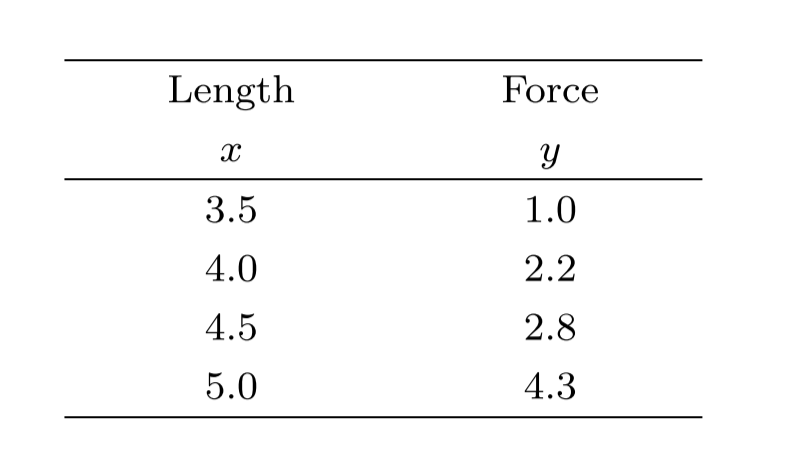
\includegraphics[width=8cm]{images/table-for-exersice-6-3-21.png}
\end{center}
\end{exercise}

\begin{proof}
\end{proof}

\begin{exercise} \label{exercise 6.3.22}
Find the \emph{minimal} solution to each of the following systems of linear equations.
\begin{enumerate}
\item
\[
    x + 2y - z = 12.
\]
\item
\[
    \sysdelim..\systeme{
        x + 2y - z = 1,
        2x + 3y + z = 2,
        4x + 7y - z = 4.
    }
\]
\item
\[
    \sysdelim..\systeme{
        x + y - z = 0,
        2x - y + z = 3,
        x - y + z = 2.
    }
\]
\item 
\[
    \sysdelim..\systeme{
        x + y + z - w =1,
        2x - y + w = 1,
        2x - y + w = 1.
    }
\]
\end{enumerate}
\end{exercise}

\begin{proof}
\end{proof}

\begin{exercise} \label{exercise 6.3.23}
Consider the problem of finding the least squares line \(y = ct + d\) corresponding to the \(m\) observations \((t_1, y_1), (t_2, y_2), ..., (t_m, y_m)\).
\begin{enumerate}
\item Show that the equation \((A^* A) x_0 = A^*y\) of \THM{6.12} takes the form of the \emph{normal equations}:
\[
    \left( \sum_{i = 1}^m t_i^2 \right) c
    + \left( \sum_{i = 1}^m t_i \right) d
    = \sum_{i = 1}^m t_i y_i
\]
and
\[
    \left( \sum_{i = 1}^m t_i \right) c + md
    = \sum_{i = 1}^m y_i.
\]
These equations may also be obtained from the error \(E\) by setting the \textbf{partial derivatives of \(E\)} with respect to both \(c\) and \(d\) equal to zero.

\item
Use the second normal equation of (a) to show that the least squares line must pass through the \emph{center of mass}, \((\overline{t}, \overline{y})\), where
\[
    \overline{t} = \frac{1}{m} \sum_{i = 1}^m t_i
    \quad \text{ and } \quad
    \overline{y} = \frac{1}{m} \sum_{i = 1}^m y_i.
\]
\end{enumerate}
\end{exercise}

\begin{proof}
\end{proof}

\begin{exercise} \label{exercise 6.3.24}
Let \(\V\) and \(\{ e_1, e_2, ... \}\) be defined as in \EXEC{6.2.23}.
Define \(\T : \V \to \V\) by
\[
    \T(\sigma)(k) = \sum_{i = 1}^{\infty} \sigma(i) \quad  \text{for every positive integer} k.
\]
Notice that the infinite series in the definition of \(\T\) \emph{converges} because \(\sigma(i) \ne 0\) for only \emph{finitely} many \(\i\).
\begin{enumerate}
\item Prove that \(\T\) is a linear operator on \(\V\).
\item Prove that for any positive integer \(n\), \(\T(e_n) = \sum_{i = 1}^n e_i.\)
\item Prove that \textbf{\(\T\) has no adjoint}.
\emph{Hint}: By way of contradiction, suppose that \(\T^*\) exists.
Prove that for any positive integer \(n\), \(\T^*(e_n)(k) \ne 0\) for infinitely many \(k\).
\end{enumerate}
\end{exercise}

\begin{proof}
\end{proof}

\section{Normal and Self-Adjoint Operators} \label{sec 6.4}

We have seen the importance of diagonalizable operators in \CH{5}.
For an operator on a vector space \(\V\) to be diagonalizable, (by \THM{5.1}) it is necessary and sufficient for \(\V\) to contain a basis of eigenvectors for this operator.
As \(\V\) is an inner product space in this chapter, \emph{it is reasonable to seek conditions that guarantee that \(\V\) has an \textbf{orthonormal} basis of eigenvectors}.
A very important result that helps achieve our goal is Schur's theorem (\THM{6.14}).
The formulation that follows is in terms of linear operators.
The next section contains the more familiar matrix form.
We begin with a lemma.

\begin{note}
小總結,這一節探討的是一個線性算子可用\textbf{標準正交基底}來對角化的充分必要條件,並且把複數內積空間跟實數內積空間分開討論。
但這個對角化實際上比第五章來地嚴格。意思是說,就算有一個線性算子不符合這些充分必要條件,也不代表他不能被對角化,很多時候它可以被對角化,只是對應的基底不是正交的。
\end{note}

\begin{lemma} \label{lem 6.4}
Let \(\T\) be a linear operator on a \emph{finite}-dimensional inner product
space \(\V\).
If \(\T\) has an eigenvector, then so does \(\T^*\).
\end{lemma}

\begin{proof}
Suppose that \(v\) is an eigenvector \textbf{of \(\T\)} with corresponding eigenvalue \(\lambda\);
that is, \(\T(v) = \lambda v\) and hence \((\T - \lambda\ITRAN{})(v) = \OV\). \MAROON{(1)}
Then for any \(x \in \V\),
\begin{align*}
    0 & = \LG \OV, x \RG & \text{by \THM{6.1}(c)} \\
      & = \LG (\T - \lambda\ITRAN{})(v), x \RG & \text{by \MAROON{(1)}} \\
      & = \LG v, (\T - \lambda\ITRAN{})^*(x) \RG & \text{by \THM{6.9}} \\
      & = \LG v, (\T^* - \conjugatet{\lambda} \ITRAN{})(x) \RG, & \text{by \THM{6.11}(a)(b)(e)}
\end{align*}
hence \(v\) is orthogonal to the \emph{range} of \(\T^* - \conjugatet{\lambda} \ITRAN{}\), so by \DEF{6.7}, \(v \in \RANGE(\T^* - \conjugatet{\lambda} \ITRAN{})^{\perp}\).
But since \(v \ne \OV\), so (since \(\RANGE(\T^* - \conjugatet{\lambda} \ITRAN{}) \cap \RANGE(\T^* - \conjugatet{\lambda} \ITRAN{})^{\perp} = \{ \OV \}\),) \(v \notin \RANGE(\T^* - \conjugatet{\lambda} \ITRAN{})\).
Then this implies \(\T^* - \conjugatet{\lambda} \ITRAN{}\) is not onto, (since there exists a vector that is not in its range) hence (by \THM{2.5}) is not one-to-one.
So there exists a nonzero vector \(u\) such that \(\T^* - \conjugatet{\lambda} \ITRAN{} (u) = \OV\), which implies \(\T^*(u) = \conjugatet{\lambda} u\), so \(u\) is an eigenvector of \(\T^*\) with corresponding eigenvalue \(\conjugatet{\lambda}\).
\end{proof}

Recall \DEF{5.14} that a subspace \(\W\) of \(\V\) is said to be \(\T\)-invariant if \(\T(\W)\) is contained in \(\W\).
If \(\W\) is \(\T\)-invariant, we may define the restriction \(\T_\W : \W \to \W\) by \(\T_\W(x) = \T(x)\) for all \(x \in \W\).
It is clear that \(\T_\W\) is a linear operator on \(\W\).
Recall from \DEF{5.5} that a polynomial is said to \textbf{split} if it factors into \emph{linear} polynomials.

\begin{theorem} [Schur] \label{thm 6.14}
Let \(\T\) be a linear operator on a \emph{finite}-dimensional inner product space \(\V\).
Suppose that the \CPOLY{} of \(\T\) splits.
Then there exists an \textbf{orthonormal} basis \(\gamma\) for \(\V\) such that the matrix \([\T]_{\gamma}\) is \textbf{upper triangular}.
\end{theorem}

\begin{proof}
Since the \CPOLY{} of \(\T\) splits, by \EXEC{5.2.12}(a), there exists an ordered basis \(\beta = \{ w_1, w_2, ..., w_n \}\) for \(\V\) such that \([\T]_{\beta}\) is upper triangular.
Now apply the Gram-Schmidt process (\THM{6.4}) to \(\beta\) to obtain an ortho\emph{gonal} basis \(\beta' = \{ v_1, v_2, ..., v_n \}\) for \(\V\).
For each \(k\), \(1 \le k \le n\), let
\[
    S_k = \{ w_1, w_2, ..., w_k \} \quad \text{ and } \quad S'_k = \{ v_1, v_2, ..., v_k \}.
\]
As in the proof of \THM{6.4}, \(\spann(S_k) = \spann(S'_k)\) for all \(k\). \MAROON{(1)}
By \EXEC{2.2.12}, (since \([\T]_{\beta}\) is upper triangular,) \(\T(w_k) \in \spann(S_k)\) for all \(k\). \MAROON{(2)}
So by \MAROON{(1)(2)}, \(\T(v_k) \in \spann(S'_k)\) for all \(k\), and by \EXEC{2.2.12} again, \([\T]_{\beta'}\) is also upper triangular.
Finally, let \(z_i = \frac{1}{\norm{z_i}} v_i\) for all \(1 \le i \le n\) and \(\gamma = \{ z_1, z_2, ..., z_n \}\).
Then \(\gamma\) is an ortho\textbf{normal} basis for \(\V\), and \([\T]_{\gamma}\) is (of course still) upper triangular.
\end{proof}

\begin{proof} [\MAROON{Proof in the fourth edition}]
The proof is by mathematical induction \textbf{on the dimension} \(n\) of \(\V\).
The result is immediate if n = 1, since by definition an one-by-one matrix is upper triangular.

So suppose that the result is true for linear operators on \((n - 1)\)-dimensional inner product spaces whose \CPOLY{} split, for some \(n > 1\).
Now let \(\T\) be a linear operator on \(n\)-dimensional inner product space \(\V\) whose \CPOLY{} splits (hence \(\T\) has eigenvector(s)).
Then by \LEM{6.4}, we can assume that \(\T^*\) has a \emph{unit} eigenvector \(z\).
Suppose that \(\T^*(z) = \lambda z\) and that \(\W = \spann(\{ z \})\).

We first show that \(\W^{\perp}\) is \(\T\)-invariant.
So suppose \(y \in \W^{\perp}\), and suppose arbitrary \(x \in \W\), then
\begin{align*}
    \LG \T(y), x \RG & = \LG \T(y), cz \RG \text{\ for come \(c\)} & \text{since \(x \in \W = \spann(\{z\})\)} \\
        & = \LG y, \T^*(cz) \RG & \text{by \THM{6.9}} \\
        & = \LG y, c\T^*(z) \RG & \text{since \(\T^*\) is linear} \\
        & = \LG y, c \lambda z \RG \\
        & = \conjugatet{c \lambda} \LG y, z \RG & \text{by \THM{6.1}(b)} \\
        & = \conjugatet{c \lambda} \cdot 0 = 0. & \text{since \(y \in \W^{\perp}\) and \(z \in \W\)}
\end{align*}
So by \DEF{6.7}, \(\T(y) \in \W^{\perp}\), hence \(\W^{\perp}\) is \(\T\)-invariant.
By \THM{5.20} the \CPOLY{} of \(\T_{\W^{\perp}}\)
\emph{divides} the \CPOLY{} of \(\T\) and hence splits.
By \THM{6.7}(c), \(\dim(\W^{\perp}) = \dim(\V) - \dim(\W) = n - 1\), \emph{so we may apply the induction hypothesis} to \(\T_{\W^{\perp}}\) and obtain an orthonormal basis \(\gamma\) of \(\W^{\perp}\) such that \([\T_{\W^{\perp}}]_{\gamma}\) is upper triangular.
Clearly, \(\beta = \gamma \cup \{ z \}\) is an orthonormal basis for \(\V\) such that \([\T]_{\beta}\) is upper triangular.
\end{proof}

We now return to our original goal of finding an orthonormal basis of eigenvectors of a linear operator \(\T\) on a finite-dimensional inner product space \(\V\).

\begin{remark} \label{remark 6.4.1}
Note that if such an orthonormal basis \(\beta\) exists, then (by \THM{6.10}) \([\T]_{\beta}\) is a diagonal matrix, and hence \([\T^*]_{\beta} = [\T]^*_{\beta}\) is \emph{also a diagonal} matrix.
Because diagonal matrices (of course, trivially, obvious, by definition of matrix product) \emph{commute}, we conclude that \(\T\) and \(\T^*\) commute, since
\begin{align*}
    [\T\T^*]_{\beta} & = [\T]_{\beta}[\T^*]_{\beta} & \text{by \THM{2.11}} \\
        & = [\T^*]_{\beta}[\T]_{\beta} & \text{since diagonal matrices commute} \\
        & = [\T^*\T]_{\beta} & \text{by \THM{2.11}}
\end{align*}
Thus \emph{if there exists an orthonormal basis for \(\V\) consisting of eigenvectors of \(\T\), then \(\T\T^* = \T^*\T\)}.
\end{remark}

\begin{definition} \label{def 6.8}
Let \(\V\) be an inner product space, and let \(\T\) be a linear operator on \(\V\).

\BLUE{(1)} We say that \(\T\) is \textbf{normal} if \(\T\T^* = \T^*\T\).

\BLUE{(2)} An \(n \X n\) real or complex matrix \(A\) is \textbf{normal} if \(AA^* = A^*A\).
\end{definition}

\begin{remark} \label{remark 6.4.2}
It follows immediately from \THM{6.10} that \(\T\) is normal if and only if \([\T]_{\beta}\) is normal for any orthonormal basis \(\beta\).

That is, given arbitrary orthonormal basis \(\beta\),
\begin{align*}
    & \T \text{ is normal} \iff \T\T^* = \T^*\T \\
    \iff & [\T\T^*]_{\beta} = [\T^*\T]_{\beta} \\
    \iff & [\T]_{\beta} [\T^*]_{\beta} = [\T^*]_{\beta} [\T]_{\beta} & \text{by \THM{2.11}} \\
    \iff & [\T]_{\beta} ([\T]_{\beta})^* = ([\T]_{\beta})^* [\T]_{\beta} & \text{by \THM{6.10}} \\
    \iff & [\T]_{\beta} \text{ is normal}
\end{align*}
\end{remark}

\begin{note}
\(\T\) 是正規算子,若且唯若存在一個標準正交基底\ \(\beta\) 使得\ \(\T\) 在\ \(\beta\) 的矩陣代表是正規矩陣。
\end{note}

\begin{example} \label{example 6.4.1}
Let \(\T: \SET{R}^2 \to \SET{R}^2\) be \textbf{rotation} by \(\theta\), where \(0 < \theta < \pi\).
The matrix representation of \(\T\) in the standard ordered basis is given by
\[
    A = \begin{pmatrix}
        \cos \theta & -\sin \theta \\
        \sin \theta & \cos \theta
    \end{pmatrix}.
\]
Note that \(A A^* = I = A^* A\); so \(A\) is normal, and hence (by \RMK{6.4.2}), \(\T\), is normal.
\end{example}

\begin{remark} \label{remark 6.4.3}
Geometrically, in \EXAMPLE{6.4.1}, \(A^*\) can be thought as a rotation matrix that rotates \emph{counterclockwise}.
That is,
\begin{align*}
    A^* & = \begin{pmatrix}
        \cos \theta & -\sin \theta \\
        \sin \theta & \cos \theta
    \end{pmatrix}^* \\
    & = \begin{pmatrix}
        \cos \theta & \sin \theta \\
        -\sin \theta & \cos \theta
    \end{pmatrix} & \text{by \DEF{6.2}} \\
    & = \begin{pmatrix}
        \cos (-\theta) & -\sin (-\theta) \\
        \sin (-\theta) & \cos (-\theta)
    \end{pmatrix} & \text{since \(\cos\), \(\sin\) are even and odd functions, respectively}
\end{align*}
\end{remark}

\begin{example} \label{example 6.4.2}
Suppose that \(A\) is a real \emph{skew-symmetric} matrix; that is, \(A^\top = -A\).
Then \(A\) is normal because both \(A A^\top\) and \(A^\top A\) are equal to \(-A^2\).
\end{example}

Clearly, the operator \(\T\) in \EXAMPLE{6.4.1} does \emph{not} even possess one eigenvector (if the field is considered to be \(\SET{R}\)).
So in the case of a \textbf{real} inner product space, we see that \emph{normality is not sufficient to guarantee an orthonormal basis of eigenvectors}.
All is not lost, however.
We show that normality \textbf{suffices} if \(\V\) is a \textbf{complex} inner product space.
Before we prove the promised result for normal operators, we need some general properties of normal operators.

\begin{theorem} \label{thm 6.15}
Let \(\V\) be an inner product space, and let \(\T\) be a \textbf{normal} operator on \(\V\).
(We do not say that \(\V\) is finite-dimensional.)
Then the Following statements are true.
\begin{enumerate}
\item \(\norm{\T(x)} = \norm{\T^*(x)}\) for all \(x \in \V\).
\item \(\T - c\ITRAN{}\) is normal for every \(c \in F\).
\item If \(x\) is an eigenvector of \(\T\) corresponding to eigenvalue \(\lambda\), then \(x\) is also an eigenvector of \(\T^*\) corresponding to eigenvalue \(\conjugatet{\lambda}\).
That is, if \(\T(x) = \lambda x\), then \(\T^*(x) = \conjugatet{\lambda}x\).
\item If \(\lambda_1\) and \(\lambda_2\) are \emph{distinct} eigenvalues of \(\T\) with corresponding eigenvectors \(x_1\) and \(x_2\), then \(x_1\) and \(x_2\) are orthogonal.
\end{enumerate}
\end{theorem}

\begin{proof} \ 

\begin{enumerate}
\item For any \(x \in \V\), we have
\begin{align*}
    \norm{\T(x)}^2 & = \LG \T(x), \T(x) \RG \\
        & = \LG \T^*(\T(x)), x \RG = \LG \T^*\T(x), x \RG & \text{by \THM{6.9}} \\
        & = \LG \T\T^*(x), x \RG = \LG \T(\T^*(x)), x \RG & \text{since \(\T\) is normal} \\
        & = \LG \T^*(x), \T^*(x) \RG & \text{by \THM{6.9}} \\
        & = \norm{\T^*(x)}^2.
\end{align*}

\item We have
\begin{align*}
    (\T - c\ITRAN{})(\T - c\ITRAN{})^*
        & = (\T - c\ITRAN{})(\T^* - \conjugatet{c}\ITRAN{}^*) & \text{by \THM{6.11}(a)(b)} \\
        & = (\T - c\ITRAN{})(\T^* - \conjugatet{c}\ITRAN{}) & \text{by \THM{6.11}(e)} \\
        & = \T\T^* - c\ITRAN{}\T^* - \T\conjugatet{c}\ITRAN{} + \conjugatet{c}c\ITRAN{}^2 & \text{expand} \\
        & = \T\T^* - c\T^* - \conjugatet{c}\T + \abs{c}^2\ITRAN{} \quad \quad \MAROON{(b.1)} & \text{simplify}
\end{align*}
and 
\begin{align*}
    (\T - c\ITRAN{})^*(\T - c\ITRAN{})
        & = (\T^* - \conjugatet{c}\ITRAN{})(\T - c\ITRAN{}) & \text{just use previous case} \\
        & = \T^*\T - \conjugatet{c}\ITRAN{}\T - \T^*c\ITRAN{} + \conjugatet{c}c\ITRAN{}^2 & \text{expand} \\
        & = \T\T^* - \MAROON{\conjugatet{c}\T} - \RED{c\T^*} + \abs{c}^2\ITRAN{} & \text{simplify} \\
        & = \T\T^* - \RED{c\T^*} - \MAROON{\conjugatet{c}\T} + \abs{c}^2\ITRAN{} = \MAROON{(b.1)} & \text{of course}
\end{align*}

\item Suppose that \(\T(x) = \lambda x\) for some \(x \in \V\).
Let \(\U = \T - \lambda \ITRAN{}\) \MAROON{(c.1)}.
Then \(\U(x) = \T(x) - \lambda \ITRAN{}(x) = \OV\) \MAROON{(c.2)}, and \(\U\) is normal by part (b).
Thus
\begin{align*}
    0 & = \norm{\OV} = \norm{\U(x)} & \text{by \MAROON{(c.2)}} \\
      & = \norm{\U^*(x)} & \text{since \(\U\) is normal, and by part(a)} \\
      & = \norm{(\T - \lambda \ITRAN{})^*(x)} & \text{by \MAROON{(c.1)}} \\
      & = \norm{(\T^* - \conjugatet{\lambda} \ITRAN{})(x)} & \text{just use \THM{6.11}} \\
      & = \norm{\T^*(x) - \conjugatet{\lambda}(x)}, & \text{of course}
\end{align*}
So \(\T^*(x) - \conjugatet{\lambda}(x) = \OV\) hence \(\T^*(x) = \conjugatet{\lambda}(x)\).
So in particular, if \(x\) is nonzero, that is, \(x\) is an eigenvector of \(\T\) corresponding to eigenvalue \(\lambda\), then \(x\) is an eigenvector of \(\T^*\) corresponding to eigenvalue \(\conjugatet{\lambda}\).

\item Let \(\lambda_1\) and \(\lambda_2\) be \emph{distinct} eigenvalues of \(\T\) with corresponding eigenvectors \(x_1\) and \(x_2\).
Then we have
\begin{align*}
    \lambda_1 \LG x_1, x_2 \RG & = \LG \lambda_1 x_1, x_2 \RG & \text{by \DEF{6.1}(a)} \\
        & = \LG \T(x_1), x_2 \RG & \text{by supposition} \\
        & = \LG x_1, \T^*(x_2) \RG & \text{by \THM{6.9}} \\
        & = \LG x_1, \conjugatet{\lambda_2} x_2 \RG & \text{by part(c), notice the conjugate} \\
        & = \conjugatet{\conjugatet{\lambda_2}} \LG x_1, x_2 \RG & \text{by \THM{6.1}(b)} \\
        & = \lambda_2 \LG x_1, x_2 \RG, & \text{by \THM{d.2}(a)}
\end{align*}
which implies \((\lambda_1 - \lambda_2) \LG x_1, x_2 \RG = 0\).
Since \(\lambda_1 \ne \lambda_2\), we conclude that \(\LG x_1, x_2 \RG = 0\), that is, \(x_1, x_2\) are orthogonal.
\end{enumerate}
\end{proof}

\begin{theorem} \label{thm 6.16}
Let \(\T\) be a linear operator on a \emph{finite}-dimensional \textbf{complex} inner product space \(\V\).
Then \(\T\) is \textbf{normal} if and only if there exists an
\textbf{orthonormal basis} for \(\V\) consisting of \textbf{eigenvectors} of \(\T\).
\end{theorem}

\begin{proof}
Suppose that \(\T\) is normal.
Since \(\V\) is over \(\SET{C}\), by the fundamental theorem of algebra (\THM{d.4}), the \CPOLY{} of \(\T\) splits.
So we may apply Schur's theorem \THM{6.14} to obtain an \emph{orthonormal} basis \(\beta = \{ v_1, v_2, ..., v_n \}\) for \(\V\) such that \([\T]_{\beta} = A\) is upper triangular.

Now We know that \(v_1\) is an eigenvector of \(\T\) because \(A\) is upper triangular.
Assume that \(v_1, v_2, ..., v_{k - 1}\) are eigenvectors of \(\T\) for some \(k > 1\).
We claim that \(v_k\) is also an eigenvector of \(\T\).
It then follows by mathematical induction on \(k\) that all of the \(v_i\)'s are eigenvectors of \(\T\).
Consider any \(j < k\), and let \(\lambda_j\) denote the eigenvalue of \(\T\) corresponding to \(v_j\).
Since \(\T\) is normal, by \THM{6.15}(c), \(\T^*(v_j) = \conjugatet{\lambda_j} v_j\). \MAROON{(1)}
Since \(A\) is upper triangular,
\begin{align*}
    \T(v_k) & = A_{1k} v_1 + A_{2k} v_2 + ... + A_{jk} v_j + ... + A_{kk}v_k + 0 \cdot v_{k + 1} + ... + 0 \cdot v_{n} \\
    & = A_{1k} v_1 + A_{2k} v_2 + ... + A_{jk} v_j + ... + A_{kk}v_k. \MAROON{(2)}
\end{align*}
Furthermore, by the \CORO{6.5.1}, since \(\beta\) is orthonormal,
\begin{align*}
    A_{jk} & = \LG \T(v_k), v_j \RG & \text{by \CORO{6.5.1}} \\
        & = \LG v_k, \T^*(v_j) \RG & \text{by \THM{6.9}} \\
        & = \LG v_k, \conjugatet{\lambda_j} v_j \RG & \text{by \MAROON{(1)}} \\
        & = \conjugatet{\conjugatet{\lambda_j}} \LG v_j, v_k \RG = \lambda_j \LG v_j, v_k \RG & \text{by \THM{6.1}(b)} \\
        & = \lambda_j \cdot 0 = 0. & \text{since \(v_j\)'s are orthonormal}
\end{align*}
So \(A_{jk} = 0\) for all \(j < k\), hence it follows from \MAROON{(2)} that \(\T(v_k) = A_{kk} v_k\), and hence \(v_k\) is an eigenvector of \(\T\).
So by induction, all the vectors in \(\beta\) are eigenvectors of \(\T\).

The converse was already proved in \RMK{6.4.1}.
\end{proof}

\begin{remark} \label{remark 6.4.4}
Interestingly, as the next example shows, \THM{6.16} does \textbf{not} extend to \textbf{infinite}-dimensional \textbf{complex} inner product spaces.
\end{remark}

\begin{example} \label{example 6.4.3}
Consider the inner product space \(\textsf{H}\) with the orthonormal set \(S\) from \EXAMPLE{6.1.9}.
Let \(\V = \spann(S)\), and let \(\T\) and \(\U\) be the linear operators on \(\V\) defined by \(\T(f) = f_1 f\) and \(\U(f) = f_{-1} f\).
Then by law of (complex) exponents,
\[
  \T(f_n)= f_{n + 1} \quad \text{ and } \quad \U(f_n) = f_{n-1} \quad \MAROON{(1)}
\]
for \emph{all} integers \(n\).
Thus
\begin{align*}
    \LG \T(f_m), f_n \RG & = \LG f_{m + 1}, f_n \RG & \text{by \MAROON{(1)}} \\
        & = \delta_{(m + 1), n} & \text{since \(S\) is orthonormal} \\
        & = \delta_{m, (n -1)} & \text{need to show, but trivial} \\
        & = \LG f_m, f_{n - 1} \RG & \text{again since \(S\) is orthonormal} \\
        & = \LG f_m, \U(f_n) \RG. & \text{by \MAROON{(1)}}
\end{align*}
It follows that \(\U = \T^*\).
Furthermore, by \MAROON{(1)}, it immediately follows that \(\T\T^* = \ITRAN{} = \T^*\T\); so \(\T\) is normal.

Now we show that \(\T\) has \textbf{no} eigenvectors.
For the sake of contradiction, suppose that \(f\) is an eigenvector of \(\T\), say, \(\T(f) = \lambda f\) for some \(\lambda\). \MAROON{(2)}
Since \(\V\) equals the span of \(S\), we may write \(f\) as a \emph{finite} linear combination of vectors in \(S\).
That is, without loss of generality, there exist integer \(n, m\) (as lower bound and upper bound for the indices of vectors we pick) such that \(n \le m\) and
\[
    f = \sum_{i = n}^m a_i f_i, \quad \text{ where } a_m \ne 0. \quad \quad \MAROON{(3)}
\]
In particular,
\begin{align*}
    \lambda \sum_{i = n}^m a_i f_i & = \lambda f & \text{by \MAROON{(3)}} \\
        & = \T(f) & \text{by \MAROON{(2)}} \\
        & = \T \left( \sum_{i = n}^m a_i f_i \right) & \text{by \MAROON{(3)}} \\
        & = \sum_{i = n}^m a_i \T(f_i) & \text{since \(\T\) is linear} \\
        & = \sum_{i = 1}^m a_i f_{i + 1} & \text{by \MAROON{(1)}}
\end{align*}
So \(\lambda \sum_{i = n}^m a_i f_i = \sum_{i = 1}^m a_i f_{i + 1}\).
Since \(a_m \ne 0\), from this equation, by moving \emph{all but the last} terms from the right side to the left side, we can write \(f_{m + 1}\) as a linear combination of \(f_n, f_{n + 1}, ..., f_m\).
But this is a \textbf{contradiction} because \(S\) is \LID{}.
\end{example}

\begin{remark} \label{remark 6.4.5}
\EXAMPLE{6.4.1} illustrates that \emph{normality is not sufficient} to guarantee the existence of an orthonormal basis of eigenvectors for \textbf{real} inner product spaces.
For real inner product spaces, we must \emph{replace normality by the stronger condition} \RED{that \(\T = \T^*\)} in order to guarantee such a basis.
\end{remark}

\begin{definition} \label{def 6.9}
Let \(\T\) be a linear operator on an inner product space \(\V\).
We say that \(\T\) is \textbf{self-adjoint} (or \textbf{Hermitian}) if \(\T = \T^*\).
An \(n \X n\) real or complex matrix \(A\) is \textbf{self-adjoint} (or \textbf{Hermitian}) if \(A = A^*\).
\end{definition}

\begin{remark} \label{remark 6.4.6}
It follows immediately that if \(\beta\) is an orthonormal basis, then (using \THM{6.10}) \(\T\) is self-adjoint if and only if \([\T]_{\beta}\) is self-adjoint.
For \textbf{real} matrices \(A\), this condition reduces to the requirement that \(A\) be \emph{symmetric}.
\end{remark}

\begin{remark} \label{remark 6.4.7}
Before we state our main result for self-adjoint operators, we need some preliminary work.
By definition, a linear operator on a real inner product space \emph{has only real eigenvalues}.
The lemma that follows shows that \emph{the same can be said} for self-adjoint operators on a \textbf{complex} inner product space.
Similarly, the \CPOLY{} of every linear operator on a \textbf{complex} inner product space splits, and \emph{the same is true} for \textbf{self-adjoint} operators on a \textbf{real} inner product space.
\end{remark}

\begin{note}
矩陣看成在複數,則特徵多項式一定\ split。
矩陣若看成在實數,但是矩陣本身\ self-adjoint,則特徵多項式也一定\ split,其中根據定義,分解後得到的根,也就是\ eigenvalues,也是實數。
\end{note}

\begin{lemma} \label{lem 6.5}
Let \(\T\) be a \textbf{self-adjoint} operator on a \emph{finite}-dimensional inner product space \(\V\).
Then
\begin{enumerate}
\item Every eigenvalue of \(\T\) is \textbf{real} (even though the inner product space is on complex field).
\item Suppose that \(\V\) is a \textbf{\RED{real}} inner product space.
Then the \CPOLY{} of \(\T\) splits (over \(\SET{R}\)).
\end{enumerate}
\end{lemma}

\begin{proof} \ 

\begin{enumerate}
\item Suppose that \(\T(x) = \lambda x\) for \(x \ne \OV\).
Because a self-adjoint operator is (of course by definition) also normal, we can apply \THM{6.15}(c) to obtain
\begin{align*}
    \lambda x & = \T(x) \\
        & = \T^*(x) & \text{since \(\T\) is self-adjoint} \\
        & = \conjugatet{\lambda} x, & \text{by \THM{6.15}(c)}
\end{align*}
which implies \(\lambda = \conjugatet{\lambda}\);
that is, (by \THM{d.2}(e)), \(\lambda\) is real.

\item Let \(n = \dim(\V)\), \(\beta\) be an \emph{orthonormal} basis for \(\V\), and \(A = [\T]_{\beta}\).
Then (by \RMK{6.4.6}) \(A\) is self-adjoint.
Let \(\T_A\) be the linear operator \RED{on \(\SET{C}^n\)} defined by \(\T_A(x) = Ax\) for all \(x \in \SET{C}^n\).
Because (by \THM{2.15}(a)) \([\T_A]_{\gamma} = A\), where \(\gamma\) is the standard ordered (orthonormal) basis for \(\SET{C}^n\), (by \RMK{6.4.6} again) \(\T_A\) is also self-adjoint.
So, by part(a), the eigenvalues of \(\T_A\) are \textbf{real}.
By the fundamental theorem of algebra, the
\CPOLY{} of \(\T_A\) splits (over \(\SET{C}\)) into factors of the form \(t - \lambda\).
\emph{But since each \(\lambda\) is real}, the \CPOLY{} splits \RED{over \(\SET{R}\)}.
But \(\T_A\) (by \DEF{5.4}) has the same \CPOLY{} as \(A\), which (again by \DEF{5.4}) has the same \CPOLY{} as \(\T\).
Therefore the \CPOLY{} of \(\T\) splits (over \(\SET{R}\)).
\end{enumerate}
\end{proof}

We are now able to establish one of the major results of this chapter.

\begin{theorem} \label{thm 6.17}
Let \(\T\) be a linear operator on a \emph{finite}-dimensional \textbf{real} inner product space \(\V\).
Then \(\T\) is \textbf{self-adjoint} if and only if there exists an \textbf{orthonormal} basis \(\beta\) for \(\V\) \textbf{consisting of eigenvectors} of \(\T\).
\end{theorem}

\begin{proof}
Suppose that \(\T\) is self-adjoint.
By \LEM{6.5}(b), the \CPOLY{} of \(\T\) \emph{splits} (over \(\SET{R}\)),
so we may apply Schur's theorem(\THM{6.14}) to obtain an \emph{orthonormal} basis \(\beta\) for \(\V\) such that the matrix \(A = [\T]_{\beta}\) is upper triangular.
But
\begin{align*}
    A^* & = ([\T]_{\beta})^* = [\T^*]_{\beta} & \text{by \THM{6.10}} \\
        & = [\T]_{\beta} & \text{since \(\T\) is self-adjoint} \\
        & = A,
\end{align*}
which implies \(A\) and \(A^*\) are both upper triangular.
But (trivially) that only happens when \(A\) is in fact a diagonal matrix.
Thus \(\beta\) must consist of eigenvectors of \(\T\).

Now suppose there exists a basis \(\beta\) for \(\V\) (over \(\SET{R}\)) such that it is orthonormal and consists of eigenvectors of \(\T\).
Then in particular, \(A = [\T]_{\beta}\) \MAROON{(1)} is a diagonal matrix, and the diagonal entries, by \CH{5}, are eigenvalues of \(\T\), which implies \emph{they must be real numbers}, hence we have \(A^* = A\). \MAROON{(2)}
But that implies
\begin{align*}
    [\T^*]_{\beta} & = ([\T]_{\beta})^* & \text{by \THM{6.10}} \\
        & = A^* & \text{by \MAROON{(1)}} \\
        & = A & \text{by \MAROON{(2)}} \\
        & = [\T]_{\beta}, & \text{by \MAROON{(1)} again}
\end{align*}
which implies \(\T^* = \T\), hence \(\T\) is self-adjoint.
\end{proof}

\begin{example} \label{example 6.4.4}
As we noted earlier, \emph{real} symmetric matrices are self-adjoint, and self-adjoint matrices are normal.
The following matrix \(A\) is \emph{complex} and symmetric:
\[
    A = \begin{pmatrix} \iu & \iu \\ \iu & 1 \end{pmatrix} \quad \text{ and } \quad A^* = \begin{pmatrix} -\iu & -\iu \\ -\iu & 1 \end{pmatrix}.
\]
But \(A\) is \emph{not} normal, because \((AA^*)_{12} = 1 + \iu\) and \((A^*A)_{12} = 1 - \iu\).
Therefore complex symmetric matrices need not be normal.
\end{example}

\exercisesection

\begin{exercise} \label{exercise 6.4.1}
Label the following statements as true or false.
Assume that the underlying inner product spaces are \emph{finite}-dimensional.
\begin{enumerate}
\item Every self-adjoint operator is normal.
\item Operators and their adjoints have the same eigenvectors.
\item If \(\T\) is an operator on an inner product space \(\V\), then \(\T\) is normal if and only if \([\T]_{\beta}\) is normal, where \(\beta\) is \emph{any} ordered basis for \(\V\).
\item A real or complex matrix \(A\) is normal if and only if \(\LMTRAN_A\) is normal.
\item The eigenvalues of a self-adjoint operator must all be real.
\item The identity and zero operators are self-adjoint.
\item Every normal operator is diagonalizable.
\item Every self-adjoint operator is diagonalizable.
\end{enumerate}
\end{exercise}

\begin{proof} \ 

\begin{enumerate}
\item True, since
\begin{align*}
    \T \RED{\T^*} & = \BLUE{\T} \RED{\T} & \text{since \(\RED{\T^*} = \RED{\T}\)} \\
        & = \BLUE{\T^*} \T & \text{since \(\BLUE{\T} = \BLUE{\T^*}\)}
\end{align*}

\item False.
Counterexample, let \(A = \begin{pmatrix} 1 & 1 \\ 0 & 1 \end{pmatrix}\) hence \(A^* = \begin{pmatrix} 1 & 0 \\ 1 & 1 \end{pmatrix}\), then we have \(\begin{pmatrix} 1 \\ 0 \end{pmatrix}\) as \(\LMTRAN_A\)'s eigenvector but not as \((\LMTRAN_A)^* = \LMTRAN_{A^*}\)'s eigenvector.

\item False, \(\beta\) should also be orthonormal.

\item True.
\(\LMTRAN_A\) is normal, iff (by \RMK{6.4.2}) \([\LMTRAN_A]_{\beta}\) is normal where \(\beta\) is the standard ordered (orthonormal) basis for \(F^n\), if and only if (by \THM{2.15}(a)) \(A\) is normal.

\item True by \LEM{6.5}(a).
\item True, since (by \THM{6.11}(d)) \(\ITRAN{}^* = \ITRAN{}\) and (similarly) \(\TZERO^* = \TZERO\).

\item False, a counterexample is \EXAMPLE{6.4.1}, the rotation transformation (over \(\SET{R}\)).

\item True.
For \emph{complex} inner product space, since (by part(a)) self-adjoint implies normal, by \THM{6.16}, we can find a orthonormal basis \(\beta\) such that the matrix representation of the operator using \(\beta\) is diagonal.
For \emph{real} inner product space, the same result is guaranteed by \THM{6.17}.
\end{enumerate}
\end{proof}

\begin{exercise} \label{exercise 6.4.2}
For each linear operator \(\T\) on an inner product space \(\V\), determine whether \(\T\) is normal, self-adjoint, or neither.
If possible, produce an orthonormal basis of eigenvectors of \(\T\) for \(\V\) and list the corresponding eigenvalues.
\begin{enumerate}
\item \(\V = \SET{R}^2\) and \(\T\) is defined by \(\T(a, b) = (2a - 2b, -2a + 5b)\).
\item \(\V = \SET{R}^3\) and \(\T\) is defined by \(\T(a, b, c) = (-a + b, 5b, 4a - 2b + 5c)\).
\item \(\V = \SET{C}^2\) and \(\T\) is defined by \(\T(a, b) = (2a + \iu b, a + 2b)\).
\item \(\V = \POLYRR\) and \(\T\) is defined by \(\T(f) = f'\), where
\[
    \LG f(x), g(x) \RG = \int_0^1 f(t)g(t) dt.
\]
\item \(\V = M_{2 \X 2}(\SET{R})\) and \(\T\) is defined by \(\T(A) = A^\top\).
\item \(\V = M_{2 \X 2}(\SET{R})\) and \(\T\) is defined by \(\T \begin{pmatrix} a & b \\ c & d \end{pmatrix} = \begin{pmatrix} c & d \\ a & b \end{pmatrix}\).
\end{enumerate}
\end{exercise}

\begin{note}
If an operator is self-adjoint, then by \EXEC{6.4.1}(a) it is normal.

To find an orthonormal basis of eigenvectors of \(\T\) for \(\V\), just find an \emph{orthonormal basis for each eigenspace} and take the union of them as the desired basis.
\end{note}

\begin{proof} \ 

\begin{enumerate}
\item Let \(\beta = \{ e_1, e_2 \}\), and let  \(A = [\T]_{\beta} = \begin{pmatrix}2 & -2 \\ -2 & 5\end{pmatrix}\),
then \([\T^*]_{\beta} = \begin{pmatrix}2 & -2 \\ -2 & 5\end{pmatrix}^* = \begin{pmatrix}2 & -2 \\ -2 & 5\end{pmatrix} = A\).
So by \RMK{6.4.6}, \(\T\) is self-adjoint, hence is normal.

\item Let  \(\beta = \{ e_1, e_2, e_3 \}\), and let \(A = [\T]_{\beta} = \begin{pmatrix}-1 & 1 & 0 \\ 0 & 5 & 0 \\ 4 & -2 & 5\end{pmatrix}\), then \([\T^*]_{\beta} = A^{*} = \begin{pmatrix}-1 & 0 & 4 \\ 1 & 5 & -2 \\ 0 & 0 & 5\end{pmatrix} \neq A\), So by \RMK{6.4.6}, \(\T\) is \emph{not} self-adjoint.
And in particular, since \((A A^*)_{11} = 2\) and \((A^* A)_{11} = 17\), \(A A^* \ne A^*A\), and by \RMK{6.4.2}, \(\T\) is not normal.
So in particular, since \(\V\) is over \(\SET{R}\), by \THM{6.17}, we cannot find a orthonormal basis consisting of eigenvectors of \(\T\).

\item Let \(\beta = \{ e_1, e_2 \}\), and let \(A = [\T]_{\beta} = \begin{pmatrix} 2 & \iu \\ 1 & 2 \end{pmatrix}\).
By calculation, \(A\) is normal but not self-adjoint.
Hence (by \RMK{6.4.6} and \RMK{6.4.2}) \(\T\) is normal but not self-adjoint.
Since the \(\V\) is over \(\SET{C}\), and \(\T\) is normal, by \THM{6.16} there exists an orthonormal basis for \(\V\) consisting eigenvectors of \(\T\).
We can compute this basis as the aforementioned note, but skip, tedious.
But one such basis is
\[
    \left\{ \left( \frac{1}{\sqrt{2}}, -\frac{1}{2} + \frac{1}{2}\iu \right), \left( \frac{1}{\sqrt{2}}, \frac{1}{2} - \frac{1}{2}\iu \right) \right\}
\]

\item We have calculated a orthonormal basis with respect to this inner product on \EXEC{6.3.2}:
\[
    \beta = \{ f_1, f_2, f_3 \} = \left\{ 1, 2\sqrt{3} \left( t - \frac{1}{2} \right), 6\sqrt{5} \left( t^2 - t + \frac{1}{6} \right) \right\}.
\]
And
\begin{align*}
    \T(f_1) & = 0 = 0 \cdot f_1 + 0 \cdot f_2 + 0 \cdot f_3 \\
    \T(f_2) & = 2\sqrt{3} = 2\sqrt{3} \cdot f_1 + 0 \cdot f_2 + 0 \cdot f_3 \\
    \T(f_3) & = 12\sqrt{5}t - 6\sqrt{5} = 0 \cdot f_1 + 2\sqrt{15} \cdot f_2 + 0 \cdot f_3 \\
    \implies &
    [\T]_{\beta} = \begin{pmatrix}
        0 & 2\sqrt{3} & 0 \\
        0 & 0 & 2\sqrt{15} \\
        0 & 0 & 0
    \end{pmatrix}
\end{align*}
So by calculation, \([\T]_{\beta}\) is neither self-adjoint nor normal, hence (by \RMK{6.3.6} and \RMK{6.3.2}) \(\T\) is neither self-adjoint nor normal.
So in particular, since \(\V\) is over \(\SET{R}\), by \THM{6.17}, we cannot find an orthonormal basis consisting of eigenvectors of \(\T\).

\item Let \(\beta = \{ E_{11}, E_{12}, E_{21}, E_{22} \}\) the ``standard'' ordered basis.
Note that the ``standard'' inner product on matrix is Frobenius inner product(\ADEF{6.1}), and \(\beta\) is orthonormal with respect to this inner product.
Then, of course,
\[
    [\T]_{\beta} = \begin{pmatrix}
        1 & 0 & 0 & 0 \\
        0 & 0 & 1 & 0 \\
        0 & 1 & 0 & 0 \\
        0 & 0 & 0 & 1
    \end{pmatrix},
\]
which by calculation is self-adjoint and normal, hence (by \RMK{6.3.6} and \RMK{6.3.2}) \(\T\) is both self-adjoint and normal.
Since the \(\V\) is over \(\SET{R}\), and \(\T\) is self-adjoint, by \THM{6.17} there exists an orthonormal basis for \(\V\) consisting eigenvectors of \(\T\).
We can compute this basis as the aforementioned note, but skip, tedious.
But one such basis is
\[
    \left\{ (1,0,0,0), \frac{1}{\sqrt{2}}(0,1,1,0),(0,0,0,1), \frac{1}{\sqrt{2}}(0,1,-1,0)\right \}
\]

\item Pick \(\beta\) as part(e), then, of course,
\[
    [\T]_{\beta} = \begin{pmatrix}
        0 & 0 & 1 & 0 \\
        0 & 0 & 0 & 1 \\
        1 & 0 & 0 & 0 \\
        0 & 1 & 0 & 0
    \end{pmatrix},
\]
which by calculation is self-adjoint and normal, hence (by \RMK{6.3.6} and \RMK{6.3.2}) \(\T\) is both self-adjoint and normal.
Since the \(\V\) is over \(\SET{R}\), and \(\T\) is self-adjoint, by \THM{6.17} there exists an orthonormal basis for \(\V\) consisting eigenvectors of \(\T\).
We can compute this basis as the aforementioned note, but skip, tedious.
But one such basis is
\[
    \left\{\frac{1}{\sqrt{2}}(1,0,-1,0), \frac{1}{\sqrt{2}}(0,1,0,-1), \frac{1}{\sqrt{2}}(1,0,1,0), \frac{1}{\sqrt{2}}(0,1,0,1)\right\}
\]
\end{enumerate}
\end{proof}

\begin{exercise} \label{exercise 6.4.3}
Give an example of a linear operator \(\T\) on \(\SET{R}^2\) and an \emph{ordered basis}(but not orthonormal) for \(\SET{R}^2\) that provides a \emph{counterexample} to the statement in \EXEC{6.4.1}(c).
\end{exercise}

\begin{proof}
Let \(\T(a, b) = (2a, b)\), and \(\beta = \{ (1, 1), (1, 0) \}\).
In particular for \(\alpha\) be the standard ordered (orthonormal) basis, \([\T]_{\alpha} = \begin{pmatrix} 2 & 0 \\ 0 & 1 \end{pmatrix}\), which is symmetric hence of course normal, hence (by \RMK{6.3.2}) \(\T\) is normal.
But \([\T]_{\beta} = \begin{pmatrix} 1 & 0 \\ 1 & 2 \end{pmatrix}\), which is \emph{not} normal.

Furthermore, the converse is also not true;
that is, we can find an operator \(\T\), which is not normal, but we can find an ordered basis \(\beta\) such that \([\T]_{\beta}\) is normal.
The process is similar.
\end{proof}

\begin{exercise} \label{exercise 6.4.4}
Let \(\T\) and \(\U\) be self-adjoint operators on an inner product space \(\V\).
Prove that \(\T\U\) is self-adjoint if and only if \(\T\U = \U\T\).
\end{exercise}

\begin{note}
根據這個陳述可知,兩個\ self-adjoint 的算子的合成\textbf{不一定}會是\ self-adjoint。
\end{note}

\begin{proof}
Suppose \(\T\U\) is self-adjoint.
Then
\begin{align*}
    \T\U & = (\T\U)^* & \text{since \(\T\U\) is self-adjoint} \\
        & = \U^*\T^* & \text{by \THM{6.11}(c)} \\
        & = \U\T^* = \U\T. & \text{since \(\T\) and \(\U\) are self-adjoint}
\end{align*}

Now suppose \(\T\U = \U\T\).
Then
\begin{align*}
    (\T\U)^* & = \U^*\T^* & \text{by \THM{6.11}(c)} \\
        & = \U\T^* = \U\T & \text{since \(\T\) and \(\U\) are self-adjoint} \\
        & = \T\U & \text{since \(\T\U = \U\T\)}
\end{align*}
Hence \(\T\U\) is self-adjoint.
\end{proof}

\begin{exercise} \label{exercise 6.4.5}
Prove \THM{6.15}(b).
\end{exercise}

\begin{proof}
See \THM{6.15}.
\end{proof}

\begin{exercise} \label{exercise 6.4.6}
Let \(\V\) be a \emph{complex} inner product space, and let \(\T\) be a linear operator on \(\V\).
Define
\[
    \T_1 = \frac{1}{2}(\T + \T^*) \quad \text{ and } \quad \T_2 = \frac{1}{2\MAROON{\iu}} (\T - \T^*).
\]
\begin{enumerate}
\item Prove that \(\T_1\) and \(\T_2\) are self-adjoint and that \(\T = \T_1 + \iu \T_2\).
\item Suppose also that \(\T = \U_1 + \iu\U_2\), where \(\U_1\) and \(\U_2\) are self-adjoint.
Prove that \(\U_1 = \T_1\) and \(\U_2 = \T_2\).
(Hence the representation is unique.)
\item Prove that \(\T\) is normal if and only if \(\T_1 \T_2 = \T_2 \T_1\).
\end{enumerate}
\end{exercise}

\begin{proof}
There is a related \EXEC{6.1.21}.
\begin{enumerate}
\item
We have
\begin{align*}
    (\T_1)^* & = \left[ \frac{1}{2}(\T + \T^*) \right]^* \\
        & = \conjugatet{\left(\frac{1}{2}\right)} (\T + \T^*)^* = \frac{1}{2} (\T + \T^*)^*& \text{by \THM{6.11}(b)} \\
        & = \frac{1}{2} (\T^* + (\T^*)^*) & \text{by \THM{6.11}(a)} \\
        & = \frac{1}{2} (\T^* + \T) = \frac{1}{2} (\T + \T^*) & \text{by \THM{6.11}(d)} \\
        & = \T_1
\end{align*}
and
\begin{align*}
    (\T_2)^* & = \left[ \frac{1}{2\iu}(\T - \T^*) \right]^* \\
        & = \conjugatet{\left(\frac{1}{2\iu}\right)} (\T - \T^*)^* = -\frac{1}{2\iu} (\T - \T^*)^*& \text{by \THM{6.11}(b)} \\
        & = -\frac{1}{2\iu} (\T^* - (\T^*)^*) & \text{by \THM{6.11}(a)} \\
        & = -\frac{1}{2\iu} (\T^* - \T) = \frac{1}{2\iu} (\T - \T^*) & \text{by \THM{6.11}(d)} \\
        & = \T_2
\end{align*}
Finally,
\begin{align*}
    \T_1 + \iu \T_2 & = \frac{1}{2}(\T + \T^*) + \iu \cdot \frac{1}{2\MAROON{\iu}} (\T - \T^*) \\
        & = \frac{1}{2}(\T + \T^*) + \frac{1\iu}{2\iu} (\T - \T^*) \\
        & =\frac{1}{2}(\T + \T^*) + \frac{1}{2} (\T - \T^*)
        = \T.
\end{align*}

\item Suppose \(\T = \U_1 + \iu \U_2\) where \(\U_1\) and \(\U_2\) are self-adjoint.
In particular,
\begin{align*}
    \T^* & = (\U_1 + \iu \U_2)^* \\
        & = \U_1^* + \conjugatet{\iu} \U_2^* = \U_1^* - \iu \U_2^* & \text{by \THM{6.11}(b)} \\
        & = \U_1 - \iu \U_2 & \text{since \(\U_1, \U_2\) are self-adjoint} \\
    \implies & \T + \T^* = (\U_1 + \iu \U_2) + (\U_1 - \iu \U_2) = 2 \U_1 \\
    \implies & \U_1 = \frac{1}{2} (\T + \T^*) = \T_1. & \text{by def of \(\T_1\)}
\end{align*}
Similarly,
\begin{align*}
    \T - \T^* & = (\U_1 + \iu \U_2) - (\U_1 - \iu \U_2) = 2\iu \U_2 \\
    \implies & \U_2 = \frac{1}{2\iu} (\T - \T^*) = \T_2. & \text{by def of \(\T_2\)}
\end{align*}
Hence the representation that \(\T = \T_1 + \iu \T_2\) is unique.

\item By tedious but skipped calculation, we have the equation
\[
    \T_1\T_2 - \T_2\T_1 = ... = \frac{1}{2\iu} (\T^*\T - \T\T^*).
\]
Then from this equation it's clear that \(\T_1\T_2 = \T_2\T_1\) if and only if \(\T^*\T = \T\T^*\), that is, if and only if \(\T\) is normal.
\end{enumerate}
\end{proof}

\begin{exercise} \label{exercise 6.4.7}
Let \(\T\) be a linear operator on an inner product space \(\V\), and let \(\W\) be a \(\T\)-invariant subspace of \(\V\).
Prove the following results.
\begin{enumerate}
\item If \(\T\) is self-adjoint, then \(\T_\W\) is self-adjoint.
\item \(\W^{\perp}\) is \(\T^{\RED{*}}\)-invariant.
\item If \(\W\) is both \(\T\)- and \(\T^*\)-invariant, then \((\T_\W)^* = (\T^*)_\W\).
\item If \(\W\) is both \(\T\)- and \(\T^*\)-invariant and \(\T\) is normal, then \(\T_\W\) is normal.
\end{enumerate}
\end{exercise}

\begin{proof}
Although \(\V\) (and \(\W\)) may be infinite-dimensional, by \RMK{6.3.4}, we assume the existence of the adjoint of any linear operators.

Note that \(\W\) itself can be seen as an inner product space, using the inner product defined on \(\V\).
\begin{enumerate}
\item Suppose \(\T\) is self-adjoint, we have to show \(\T_\W = (\T_\W)^*\).
Then for any \(x, y \in \W\),
\begin{align*}
    \LG x, (\T_\W)^*(y) \RG & = \LG \T_\W(x), y \RG & \text{by \THM{6.9}} \\
        & = \LG \T(x), y \RG & \text{by def of \(\T_\W\)} \\
        & = \LG x, \T^*(y) \RG & \text{by \THM{6.9} again} \\
        & = \LG x, \T(y) \RG & \text{since \(\T\) is self-adjoint} \\
        & = \LG x, \T_\W(y) \RG & \text{by def of \(\T_\W\)}
\end{align*}
which (by \THM{6.1}(e)) implies \((\T_\W)^*(y) = \T_\W(y)\) for all \(y \in \W\), hence \((\T_\W)^* = \T_\W\).

\item Suppose \(x \in \W^{\perp}\), we have to show \(\T^*(x) \in \W^{\perp}\).
To do this, (by \DEF{6.7}) we can show that \(\LG \T^*(x), y \RG = 0\) for all \(y \in \W\).
But for all \(y \in \W\),
\begin{align*}
    \LG \T^*(x), y \RG & = \LG \T(x), y \RG & \text{since \(\T\) is self-adjoint} \\
        & = \LG x, \T^*(y) \RG & \text{by \THM{6.9}} \\
        & = \LG x, \T(y) \RG & \text{since \(\T\) is self-adjoint} \\
        & = 0, &
\end{align*}
where the last step is because that \(\T(y) \in \W\) (since \(y \in \W\) and \(\W\) is \(\T\)-invariant) and \(x \in \W^{\perp}\).
Hence \(\T^*(x) \in \W^{\perp}\), so \(\W^{\perp}\) is \(\T^*\)-invariant.

\item (By the assumption that \(\W\) is \(\T^*\)-invariant, the notation \((\T^*)_\W\) now does make sense.)
For all \(x, y \in \W\),
\begin{align*}
    \LG x, (\T_\W)^*(y) \RG & = \LG \T_\W(x), y \RG & \text{by \THM{6.9}} \\
        & = \LG \T(x), y \RG & \text{by def of \(\T_\W\)} \\
        & = \LG x, \T^*(y) \RG & \text{by \THM{6.9} again} \\
        & = \LG x, (\T^*)_\W(y) \RG & \text{by def of \((\T^*)_\W\)}
\end{align*}
Hence (by \THM{6.1}(e)) \((\T_\W)^*(y) = (\T^*)_\W(y)\) for all \(y \in \W\), hence \((\T_\W)^* = (\T^*)_\W\).

\item We have to show \((\T_\W)^* \T_\W = \T_\W (\T_\W)^*\).
And for all \(x \in \W\),
\begin{align*}
    (\T_\W)^* \T_\W(x) & = \RED{(\T^*)_\W} \T_\W(x) & \text{by part(c)} \\
        & = \T^* \T (x) & \text{by def of \((\T^*)_\W\) and \(\T_\W\)} \\
        & = \T \T^* (x) & \text{since \(\T\) is normal} \\
        & = \T_\W (\T^*)_\W (x) & \text{by def of \(\T_\W\) and \((\T^*)_\W\) again} \\
        & = \T_\W \RED{(\T_\W)^*} (x) & \text{by part(c)}
\end{align*}
Hence \((\T_\W)^* \T_\W = \T_\W (\T_\W)^*\), as desired.
\end{enumerate}
\end{proof}

\begin{exercise} \label{exercise 6.4.8}
Let \(\T\) be a \emph{normal} operator on a \emph{finite}-dimensional \textbf{complex} inner product space \(\V\), and let \(\W\) be a subspace of \(\V\).
Prove that if \(\W\) is \(\T\)-invariant, then \(\W\) is also \(\T^*\)-invariant.
\emph{Hint}: Use \EXEC{5.4.24}.
\end{exercise}

\begin{proof}
Since \(\V\) is over \(\SET{C}\) and \(\T\) is normal, by \THM{6.16} there exists an orthonormal basis consisting of eigenvectors of \(\V\).
In particular, \(\T\) is diagonalizable, and by \EXEC{5.4.24}, \(\T_\W\) is diagonalizable.
So let \(\beta_\W = \{ v_1, v_2, ..., v_k \}\) be the basis for \(\W\) and consist of eigenvectors of \(\T_\W\).
Then in particular, \(v_1, ..., v_k\) are eigenvectors of \(\T\); and we can let the corresponding eigenvalues as \(\lambda_1, ..., \lambda_k\).
By \THM{6.15}(c), \(v_1, ..., v_k\) are eigenvectors of \(\T^*\) corresponding to \(\conjugatet{\lambda_1}, ..., \conjugatet{\lambda_k}\).

Now we show that \(\W\) is \(\T^*\)-invariant, that is, if \(v \in \W\), then \(\T^*(v) \in \W\).
So let \(v \in \W\).
Since \(\beta_\W\) is a basis for \(\W\), we can let \(v = a_1 v_1 + ... + a_k v_k\) for some coefficients \(a_1, ..., a_k\), and
\begin{align*}
    \T^*(v) & = \T^*(a_1 v_1 + ... + a_k v_k) \\
        & = a_1 \T^* (v_1) + ... + a_k \T^* (v_k) & \text{since \(\T^*\) is linear} \\
        & = a_1 \conjugatet{\lambda_1} v_1 + ... + a_k \conjugatet{\lambda_k} v_k
\end{align*}
which is still a linear combination of \(v_1, ..., v_k\) hence is in \(\W\).
So \(\T^*\) is \(\W\)-invariant.
\end{proof}

\begin{exercise} \label{exercise 6.4.9}
Let \(\T\) be a \emph{normal} operator on a \emph{finite}-dimensional inner product space \(\V\).
Prove that \(\NULLT = \NULL(\T^*)\) and \(\RANGET = \RANGE(\T^*)\).
\emph{Hint}: Use \THM{6.15} and \EXEC{6.3.12}.
\end{exercise}

\begin{note}
所以一個\ operator 如果\ normal,則它跟它的\ adjoint 的零空間還有值域都會一樣。
\end{note}

\begin{proof}
We have
\begin{align*}
    x \in \NULLT & \iff \T(x) = \OV \iff \norm{\T(x)} = 0 & \text{by \THM{6.2}(b)} \\
        & \iff \norm{\T^*(x)} = 0 & \text{since \(\T\) is normal and by \THM{6.15}(a)} \\
        & \iff \T^*(x) = \OV \iff x \in \NULL(\T^*) & \text{by \THM{6.2}(b)}
\end{align*}

Now by \EXEC{6.3.12}(b), (since \(\V\) is finite-dimensional) we have \(\RANGE(\T^*) = \NULLT^{\perp}\) for any linear operator \(\T\).
In particular, we have \(\RANGE(\RED{(\T^*)}^*) = \NULL(\RED{\T^*})^{\perp}\). \MAROON{(1)}

For the second equation \(\RANGET = \RANGE(\T^*)\), we have
\begin{align*}
    \RANGET & = \RANGE(\RED{(\T^*)}^*) & \text{by \THM{6.11}(d)} \\
        & = \NULL(\RED{\T^*})^{\perp} & \text{by \MAROON{(1)}} \\
        & = \NULL(\BLUE{\T})^{\perp} & \text{by the first equation that we have shown} \\
        & = \RANGE(\BLUE{\T}^*) & \text{by \EXEC{6.3.12}(c) again, where the operator is \(\BLUE{\T}\)}
\end{align*}
\end{proof}

\begin{exercise} \label{exercise 6.4.10}
Let \(\T\) be a \emph{self-adjoint} operator on a finite-dimensional inner product space \(\V\).
Prove that for all \(x \in \V\)
\[
    \norm{\T(x) \pm \iu x}^2 = \norm{\T(x)}^2 + \norm{x}^2.
\]
Deduce that \(\T - \iu \ITRAN{}\) is invertible and that \emph{the adjoint of} \((\T - \iu \ITRAN{})^{-1}\) is \((\T + \iu \ITRAN{})^{-1}\).
\end{exercise}

\begin{proof}
We have
\begin{align*}
    \norm{\T(x) + \iu x}^2
        & = \LG \T(x) + \iu x, \T(x) + \iu x \RG & \text{by \DEF{6.3}} \\
        & = \LG \T(x), \T(x) \RG
          + \LG \T(x), \iu x \RG
          + \LG \iu x, \T(x) \RG
          + \LG \iu x, \iu x \RG \\
          & \quad \quad \quad \text{(by \THM{6.1}, \DEF{6.1}(a))} \\
        & = \norm{\T(x)}^2
          + \LG \T(x), \iu x \RG
          + \LG \iu x, \T(x) \RG
          + \norm{\iu x}^2 & \text{by \DEF{6.3}} \\
        & = \norm{\T(x)}^2 - \iu \LG \T(x), x \RG + \iu \LG x, \T(x) \RG + \norm{\iu x}^2 \\
          & \quad \quad \quad \text{(by \THM{6.1}, \DEF{6.1}(b))} \\
        & = \norm{\T(x)}^2 - \iu \LG x, \RED{\T^*}(x) \RG + \iu \LG x, \T(x) \RG + \norm{\iu x}^2 & \text{by \THM{6.9}} \\
        & = \norm{\T(x)}^2 - \iu \LG x, \RED{\T}(x) \RG + \iu \LG x, \T(x) \RG + \norm{\iu x}^2 & \text{since \(\T\) is self-adjoint} \\
        & = \norm{\T(x)}^2 + \norm{\iu x}^2 & \text{of course} \\
        & = \norm{\T(x)}^2 + \abs{\iu}^2\norm{x}^2 & \text{by \THM{6.2}(a)} \\
        & = \norm{\T(x)}^2 + \norm{x}^2 & \text{of course}
\end{align*}
Similarly,
\begin{align*}
    \norm{\T(x) - \iu x}^2
        & = \LG \T(x) - \iu x, \T(x) - \iu x \RG & \text{by \DEF{6.3}} \\
        & = \LG \T(x), \T(x) \RG
          + \LG \T(x), -\iu x \RG
          + \LG -\iu x, \T(x) \RG
          + \LG -\iu x, -\iu x \RG \\
          & \quad \quad \quad \text{(by \THM{6.1}, \DEF{6.1}(a))} \\
        & = \norm{\T(x)}^2 + \iu \LG \T(x), x \RG - \iu \LG x, \T(x) \RG + \norm{\iu x}^2 \\
          & \quad \quad \quad \text{(by \DEF{6.3}, \THM{6.1}, \DEF{6.1}(b))} \\
        & = \norm{\T(x)}^2 + \iu \LG x, \RED{\T^*}(x) \RG - \iu \LG x, \T(x) \RG + \norm{\iu x}^2 & \text{by \THM{6.9}} \\
        & = \norm{\T(x)}^2 + \iu \LG x, \RED{\T}(x) \RG - \iu \LG x, \T(x) \RG + \norm{\iu x}^2 & \text{since \(\T\) is self-adjoint} \\
        & = \norm{\T(x)}^2 + \norm{\iu x}^2 & \text{of course} \\
        & = \norm{\T(x)}^2 + \abs{\iu}^2\norm{x}^2 & \text{by \THM{6.2}(a)} \\
        & = \norm{\T(x)}^2 + \norm{x}^2 & \text{of course}
\end{align*}

In particular, \(\T - \iu \ITRAN{}\) is one-to-one, since:
\begin{align*}
         & (\T - \iu \ITRAN{}) (x) = \OV \\
    \iff & \norm{(\T - \iu \ITRAN{})(x)} = \norm{\T(x) - \iu x} = 0 & \text{by \THM{6.2}(b)} \\
    \iff & \norm{\T(x) - \iu x}^2 = 0 & \text{of course} \\
    \iff & \norm{\T(x)}^2 + \norm{x}^2 = 0 & \text{by what we have shown} \\
    \iff & \norm{\T(x)} = \norm{x} = 0 & \text{of course (by field algebra)} \\
    \iff & \T(x) = x = \OV & \text{by \THM{6.2}(b) again}
\end{align*}
Hence \((\T - \iu \ITRAN{}) (x) = \OV \iff x = \OV\), so \(\T - \iu \ITRAN{}\) is one-to-one, and  (by \THM{2.5}) invertible, so \((\T - \iu \ITRAN{})^{-1}\) exists, hence \(\left[ (\T - \iu \ITRAN{})^{-1} \right]^*\) exists.

Finally, we need to show that \((\T + \iu \ITRAN{})^{-1}\) also exists and \((\T + \iu \ITRAN{})^{-1} = \left[ (\T - \iu \ITRAN{})^{-1} \right]^*\).
And it suffices to show that \(\left[ (\T - \iu \ITRAN{})^{-1} \right]^* (\T + \iu \ITRAN{}) = (\T + \iu \ITRAN{}) \left[ (\T - \iu \ITRAN{})^{-1} \right]^* = \ITRAN{}\).

We use the ``inner product trick'' again: for any \(x, y \in \V\),
\begin{align*}
    & \quad \LG x, \left[ (\T - \iu \ITRAN{})^{-1} \right]^* (\T + \iu \ITRAN{}) (y) \RG \\
    & = \LG \left[ (\T - \iu \ITRAN{})^{-1} \right](x), (\T + \iu \ITRAN{}) (y) \RG & \text{by \THM{6.9}} \\
    & = \LG \left[ (\T - \iu \ITRAN{})^{-1} \right](x), (\RED{\T^*} + \iu \ITRAN{}) (y) \RG & \text{since \(\T\) is self-adjoint} \\
    & = \LG \left[ (\T - \iu \ITRAN{})^{-1} \right](x), (\T - \iu \ITRAN{})^* (y) \RG & \text{of course by \THM{6.11}} \\
    & = \LG (\T - \iu \ITRAN{}) \left[ (\T - \iu \ITRAN{})^{-1} \right](x), y \RG & \text{by \THM{6.9} again} \\
    & = \LG x, y \RG = \LG x, \ITRAN{}(y) \RG. & \text{of course}
\end{align*}
hence \(\left[ (\T - \iu \ITRAN{})^{-1} \right]^* (\T + \iu \ITRAN{}) (y) = \ITRAN{}(y)\) for all \(y \in \V\), so \(\left[ (\T - \iu \ITRAN{})^{-1} \right]^* (\T + \iu \ITRAN{}) = \ITRAN{}\).
The same process can be used to show that \((\T + \iu \ITRAN{}) \left[ (\T - \iu \ITRAN{})^{-1} \right]^* = \ITRAN{}\).
Hence we have \((\T + \iu \ITRAN{})^{-1} = \left[ (\T - \iu \ITRAN{})^{-1} \right]^*\).
\end{proof}
\begin{note}
\EXEC{6.4.10} 不知道有什麼用意? 給定一個\ self-adjoint \(\T\),\(\T \pm \iu \ITRAN{}\) 有什麼特別的用途嗎?
\end{note}

\begin{exercise} \label{exercise 6.4.11}
Assume that \(\T\) is a linear operator on a \emph{complex} (\emph{not necessarily finite} dimensional) inner product space \(\V\) with an adjoint \(\T^*\).
Prove the following results.
\begin{enumerate}
\item If \(\T\) is self-adjoint, then \(\LG \T(x), x \RG\) is \textbf{real} for all \(x \in \V\).
\item If \(\T\) satisfies \(\LG \T(x), x \RG = 0\) for all \(x \in \V\), then \(\T = \TZERO\).
\emph{Hint}: Replace \(x\) by \(x + y\) and then by \(x + \iu y\), and expand the resulting inner products.
\item If \(\LG \T(x), x \RG\) is real for all \(x \in \V\), then \(\T\) is self-adjoint.
\end{enumerate}
\end{exercise}

\begin{note}
Part(a) and part(c) form a if and only if statement.
And it seems that part(b) is used in \SEC{6.5} (by my professor).
\TODOREF{(which part?)}
\end{note}

\begin{proof} \ 

\begin{enumerate}
\item For all \(x \in \V\), we have
\begin{align*}
    \LG \T(x), x \RG & = \LG x, \T^*(x) \RG & \text{by \THM{6.9}} \\
        & = \LG x, \T(x) \RG & \text{since \(\T\) is self-adjoint} \\
        & = \conjugatet{\LG \T(x), x \RG} & \text{by \DEF{6.1}(c)}
\end{align*}
which by \THM{d.2}(e) implies \(\LG \T(x), x \RG\) is a real number.

\item In particular, for \(x, y \in \V\), \(x + y \in \V\) and \(x + \iu y \in \V\), so we have \(\LG \T(x + y), x + y \RG = 0\) and \(\LG \T(x + \iu y), x + \iu y \RG = 0\).
And that implies
\begin{align*}
    0 & = \LG \T(x + y), x + y \RG \\
      & = \LG \T(x) + \T(y), x + y \RG & \text{since \(\T\) is linear} \\
      & = \LG \T(x), x \RG + \LG \T(x), y \RG + \LG \T(y), x \RG + \LG \T(y), y \RG & \text{just expand} \\
      & = 0 + \LG \T(x), y \RG + \LG \T(y), x \RG + 0 & \text{since \(x \in \V\) and \(y \in \V\)} \\
    \implies & \LG \T(x), y \RG = -\LG \T(y), x \RG.
\end{align*}
and
\begin{align*}
    0 & = \LG \T(x + \iu y), x + \iu y \RG \\
      & = \LG \T(x) + \iu \T(y), x + \iu y \RG & \text{since \(\T\) is linear} \\
      & = \LG \T(x), x \RG + \LG \T(x), \iu y \RG + \LG \iu \T(y), x \RG + \LG \iu \T(y), \iu y \RG & \text{just expand} \\
      & = \LG \T(x), x \RG - \iu \LG \T(x), y \RG + \iu \LG \T(y), x \RG + \abs{\iu}^2 \LG \T(y), y \RG \\
      & \quad \quad \quad \text{(by \THM{6.1},\DEF{6.1}(b))} \\
      & = 0 - \iu \LG \T(x), y \RG + \iu \LG \T(y), x \RG + 1 \cdot 0 & \text{since \(x \in \V\) and \(y \in \V\)} \\
      & = -\iu \LG \T(x), y \RG + \iu \LG \T(y), x \RG \\
    \implies & \iu \LG \T(x), y \RG = \iu \LG \T(y), x \RG \\
    \implies & \LG \T(x), y \RG = \LG \T(y), x \RG
\end{align*}
Hence we have \(\LG \T(x), y \RG = -\LG \T(y), x \RG\) and \(\LG \T(x), y \RG = \LG \T(y), x \RG\), which implies \(-\LG \T(y), x \RG = \LG \T(y), x \RG\) and implies \(\LG \T(y), x \RG = 0\). 
In particular, \(\LG \T(x), y \RG = \LG \T(y), x \RG = 0\), and \(\LG y, \T(x) \RG = \conjugatet{\LG \T(x), y \RG} = \conjugatet{0} = 0\).

So we have for all \(x, y \in \V\), \(\LG y, \T(x) \RG = 0\), which (by \THM{6.1}(e)) implies \(\T(x) = \OV\) for all \(x\), hence \(\T = \TZERO\).

\item We have, for all \(x \in \V\),
\begin{align*}
    \LG \T(x), x \RG & = \conjugatet{\LG \T(x), x \RG} & \text{by \THM{d.2}(e)} \\
        & = \conjugatet{\LG x, \T^*(x) \RG} & \text{by \THM{6.9}} \\
        & = \LG \T^*(x), x \RG & \text{by \DEF{6.1}(c)} \\
    \implies & \LG \T(x) - \T^*(x), x \RG = 0 & \text{by \DEF{6.1}} \\
    \implies & \LG (\T - \T^*)(x), x \RG = 0 & \text{of course}
\end{align*}
By part(b), we have \(\T - \T^* = \TZERO\), hence \(\T = \T^*\).
\end{enumerate}
\end{proof}

\begin{exercise} \label{exercise 6.4.12}
Let \(\T\) be a \emph{normal} operator on a \emph{finite}-dimensional \textbf{real} inner product space \(\V\) whose \CPOLY{} \emph{splits}.
Prove that \(\V\) has an orthonormal basis of eigenvectors of \(\T\).
Hence (since \(\V\) is over \(\SET{R}\) and consists of orthonormal basis of eigenvectors of \(\T\), by \THM{6.17}, with the statement from right to left,) \(\T\) is self-adjoint.
\end{exercise}

\begin{note}
So on \emph{real} inner product space, normal and splitted-\CPOLY{} imply self-adjoint.
\end{note}

\begin{proof}
(The proof is similar to \THM{6.16}.)
Suppose \(\T\) is a normal operator on real inner product space \(\V\) such that its \CPOLY{} splits.
In particular, all eigenvalues of \(\T\) are real. \MAROON{(1)}
And by Schur's Theorem (\THM{6.14}), there exists an ordered orthonormal basis \(\beta = \{ v_1, v_2, ..., v_n \}\) such that \([\T]_{\beta}\) is upper triangular.
In particular, (sine \([\T]_{\beta}\) is upper triangular,) \(v_1\) is an eigenvector of \(\T\).
(Similar to the proof of \THM{6.16},) Assume that \(v_1, v_2, ..., v_{k - 1}\) are eigenvectors of \(\T\) for some \(k > 1\).
We claim that \(v_k\) is also an eigenvector of \(\T\).
It then follows by mathematical induction on \(k\) that all of the \(v_i\)'s are eigenvectors of \(\T\).

Consider any \(j < k\), and let \(\lambda_j\) denote the eigenvalue of \(\T\) corresponding to \(v_j\).
Since \(\T\) is normal, by \THM{6.15}(c), \(\T^*(v_j) = \conjugatet{\lambda_j} v_j\).
But (since the inner product space is over \(\SET{R}\)), by \MAROON{(1)} we have \(\conjugatet{\lambda_j} = \lambda_j\), that is, \(\T^*(v_j) = \lambda_j v_j\). \MAROON{(2)}

And since \(A\) is upper triangular,
\begin{align*}
    \T(v_k) & = A_{1k} v_1 + A_{2k} v_2 + ... + A_{jk} v_j + ... + A_{kk}v_k + 0 \cdot v_{k + 1} + ... + 0 \cdot v_{n} \\
    & = A_{1k} v_1 + A_{2k} v_2 + ... + A_{jk} v_j + ... + A_{kk}v_k. \quad \quad \MAROON{(3)}
\end{align*}
Furthermore, by the \CORO{6.5.1}, since \(\beta\) is orthonormal,
\begin{align*}
    A_{jk} & = \LG \T(v_k), v_j \RG & \text{by \CORO{6.5.1}} \\
        & = \LG v_k, \T^*(v_j) \RG & \text{by \THM{6.9}} \\
        & = \LG v_k, \lambda_j v_j \RG & \text{by \MAROON{(2)}} \\
        & = \conjugatet{\lambda_j} \LG v_j, v_k \RG = \lambda \LG v_j, v_k \RG & \text{by \THM{6.1}(b) and \MAROON{(1)}} \\
        & = \lambda_j \cdot 0 = 0. & \text{since \(v_j\)'s are orthonormal}
\end{align*}
So \(A_{jk} = 0\) for all \(j < k\), hence it follows from \MAROON{(3)} that \(\T(v_k) = A_{kk} v_k\), and hence \(v_k\) is an eigenvector of \(\T\).
So by induction, all the vectors in \(\beta\) are eigenvectors of \(\T\);
so \(\V\) has an orthonormal basis, \(\beta\), of eigenvectors of \(\T\).
\end{proof}

\begin{exercise} \label{exercise 6.4.13}
An \(n \X n\) \emph{real} matrix \(A\) is said to be a \textbf{Gramian} matrix if there exists a \emph{real} (square) matrix \(B\) such that \(A = B^\top B\).
Prove that \(A\) is a Gramian matrix if and only if \(A\) is symmetric and all of its eigenvalues are \emph{nonnegative}.
\emph{Hint}: Apply \THM{6.17} to \(\T = \LMTRAN_A\) to obtain an orthonormal basis \(\{ v_1, v_2, ..., v_n \}\)
of eigenvectors with the associated eigenvalues \(\lambda_1, \lambda_2, ..., \lambda_n\).
Define the linear operator \(\U\) by \(\U(v_i) = \sqrt{\lambda_i} v_i\).
\end{exercise}

\begin{proof}
Note that since the matrix is real, \(A^*\) is reduced to \(A^\top\).

\(\Longrightarrow\): Suppose \(A\) is Gramian such that \(A = B^\top B\) for some real square matrix \(B\).
Then we have (by the properties of matrix transpose)
\[
    A^\top = (B^\top B)^\top = B^\top (B^\top)^\top = B^\top B = A
\]
Hence \(A\) is symmetric.
Now suppose \(\lambda\) is an eigenvalue of \(A\), hence we have \(Ax = \lambda x\) for some \textbf{unit vector} \(x\).
In particular, (if we view \(Ax, Bx\) as \(\LMTRAN_A(x), \LMTRAN_B(x)\), with \THM{6.9},)
\begin{align*}
    0 & \le \LG Bx, Bx \RG & \text{of course} \\
      & = \LG x, B^* B x \RG & \text{by \THM{6.9}} \\
      & = \LG x, B^\top B x \RG & \text{since \(B\) is real matrix} \\
      & = \LG x, Ax \RG & \text{by def of \(A\)} \\
      & = \LG x, A^\top x \RG = \LG x, A^* \top \RG & \text{since \(A\) is symmetric and real} \\
      & = \LG Ax, x \RG & \text{by \THM{6.9} again} \\
      & = \LG \lambda x, x \RG & \text{by supposition} \\
      & = \lambda \LG x, x \RG & \text{by \DEF{6.1}(b)} \\
      & = \lambda \cdot 1 = \lambda & \text{since \(x\) is unit vector}.
\end{align*}
So all eigenvalues of \(A\) are nonnegative.

\(\Longleftarrow\): Now suppose \(A\) is symmetric and all eigenvalues of \(A\) are nonnegative.
In particular, since \(A\) is real and symmetric, by definition it's self-adjoint, and \(A = [\LMTRAN_A]_{\alpha}\) where \(\alpha\) is the standard ordered (orthonormal) basis, hence (by \RMK{6.4.6}) \(\LMTRAN_A\) is also self-adjoint.

So by \THM{6.17}, there exists an orthonormal basis \(\beta = \{ v_1, v_2, ..., v_n \}\) consisting eigenvectors of \(\LMTRAN_A\), in particular, \([\LMTRAN_A]_{\beta}\) is diagonal.

Now the tricky part: define \(D\) be the diagonal matrix such that its \(ii\)-entry is \(\sqrt{\lambda_i}\) where \(\lambda_i\) is the \(ii\)-entry of \([\LMTRAN_A]_{\beta}\).
Then since each \(\lambda_i\) is nonnegative, \(D\) is also a \textbf{real} matrix.
And of course \(D\) is symmetric \MAROON{(1)} and \(D^2 = [\LMTRAN_A]_{\beta}\). \MAROON{(2)}

Note that we have let \(\alpha\) be the standard ordered basis, and
\begin{align*}
    A & = [\LMTRAN_A]_{\alpha} & \text{by \THM{2.15}(a)} \\
      & = [\ITRAN{}]_{\beta}^{\alpha} [\LMTRAN_A]_{\beta} [\ITRAN{}]_{\alpha}^{\beta} & \text{by \THM{2.23}} \\
      & = [\ITRAN{}]_{\beta}^{\alpha} D^2 [\ITRAN{}]_{\alpha}^{\beta} & \text{by \MAROON{(2)}} \\
      & = ([\ITRAN{}]_{\beta}^{\alpha} D) (D [\ITRAN{}]_{\alpha}^{\beta}) & \text{of course} \\
      & = ([\ITRAN{}]_{\beta}^{\alpha} D) (D^\top) [\ITRAN{}]_{\alpha}^{\beta}) & \text{by \MAROON{(1)}}
\end{align*}
Now from \THM{2.23}, let \(Q^{-1} = [\ITRAN{}]_{\beta}^{\alpha}\), then \(Q = [\ITRAN{}]_{\alpha}^{\beta}\), so from the last equation we have \(A = (Q^{-1} D) (D^\top Q)\). \MAROON{(3)}.

Since \(Q^{-1} = [\ITRAN{}]_{\beta}^{\alpha}\), the \(j\)th column of \(Q^{-1}\) is \(v_j\), that is, the columns of \(Q^{-1}\) are the vectors of the orthonormal basis \(\beta\).
So by \EXEC{6.1.23}(c), we have \((Q^{-1})^* = (Q^{-1})^{-1} = Q\).
But since \((Q^{-1})^*\) is real matrix, the equation reduces to \((Q^{-1})^\top = Q\). \MAROON{(4)}

Hence
\begin{align*}
    A & = (Q^{-1} D) (D^\top \RED{Q}) & \text{by \MAROON{(3)}} \\
      & = (Q^{-1} D) (D^\top \RED{(Q^{-1})^\top}) & \text{by \MAROON{(4)}} \\
      & = (Q^{-1} D) (Q^{-1} D)^\top & \text{of course by the property of transpose} \\
      & = ((Q^{-1} D)^\top)^\top (Q^{-1} D)^\top. & \text{of course by the property of transpose}
\end{align*}
Hence we have found a matrix \(B = (Q^{-1} D)^\top\) such that \(A = B^\top B\);
in particular, since \(Q^{-1}\) and \(D\) are \textbf{real} matrices, \(B\) is also real matrix, hence \(A\) is a Gramian matrix, as desired.
\end{proof}

\begin{exercise} \label{exercise 6.4.14}
\emph{Simultaneous Diagonalization}.
Let \(\V\) be a finite-dimensional \textbf{real} inner product space, and let \(\U\) and \(\T\) be \textbf{self-adjoint} linear operators on \(\V\) such that \(\U\T = \T\U\).
Prove that there exists an \textbf{orthonormal} basis for \(\V\) consisting of vectors that are eigenvectors of both \(\U\) and \(\T\).
(The complex version of this result appears as \EXEC{6.6.10}.)
\emph{Hint}: For any eigenspace \(\W = E_{\lambda}\) of \(\T\), we have that \(\W\) is both \(\T\)- and \(\U\)-invariant.
By \EXEC{6.4.7}, we have that \(\W^{\perp}\) is both \(\T\)- and \(\U\)-invariant.
Apply \THM{6.17} and \THM{6.6}.
\end{exercise}

\begin{proof}
Let \(\V\) be an arbitrary \(n\)-dimensional \textbf{real} inner product space, and let \(\U\) and \(\T\) be \textbf{self-adjoint} linear operators on \(\V\) such that \(\U\T = \T\U\).

We use induction on the dimension of the underlying (real) inner product space.
So for \(n = 1\), by \EXEC{5.4.25} \(\T\) and \(\U\) can already be diagonalized simultaneously by an ordered basis.
But since the basis is a singleton set, by normalizing the vector in it, we get an orthonormal basis, hence \(\T\) and \(\U\) can be diagonalized simultaneously by an orthonormal basis.

Now suppose the statement is true for \(n \le k - 1\), where \(k > 1\);
that is, for arbitrary finite-dimensional real inner product space \(\V\) such that \(\dim(\V) \le k - 1\),
given \(\U\) and \(\T\) be \textbf{self-adjoint} linear operators on \(\V\) such that \(\U\T = \T\U\), there exists an orthonormal basis for \(\V\) consisting of vectors that are eigenvectors of both \(\U\) and \(\T\).

We have to show the statement is true for \(n = k\); that is, for arbitrary \(k\)-dimensional real inner product space \(\V\),
given \(\U\) and \(\T\) be \textbf{self-adjoint} linear operators on \(\V\) such that \(\U\T = \T\U\), there exists an orthonormal basis for \(\V\) consisting of vectors that are eigenvectors of both \(\U\) and \(\T\).

So let \(\V\) be a \(k\)-dimensional real inner product space, and let \(\U\) and \(\T\) be \textbf{self-adjoint} linear operators on \(\V\) such that \(\U\T = \T\U\).
Let assume \(\W = E_{\lambda}\) is an eigenspace corresponding to \(\lambda\) of \(\T\).
Then (by \EXAMPLE{5.4.1}) \(\W\) is \(\T\)-invariant.
Now we show that \(\W\) is also \(\U\)-invariant:
Suppose \(x \in \W\); in particular, \(\T(x) = \lambda x\). \MAROON{(1)}
Then
\begin{align*}
    \U\T = \T\U \implies & \U\T(x) = \T\U(x) \\
        \implies & \U(\T(x)) = \T(\U(x)) & \text{of course} \\
        \implies & \U(\lambda x) = \T(\U(x)) & \text{by \MAROON{(1)}} \\
        \implies & \lambda \U(x) = \T(\U(x)) & \text{since \(\U\) is linear} \\
        \implies & \U(x) \text{ is an eigenvector of \(\T\) corresponding to } \lambda
\end{align*}
So by definition, \(\U(x) \in E_{\lambda}\); that is, \(\U(x) \in \W\), hence \(\W\) is \(\U\)-invariant. \MAROON{(2)}
(BTW the same strategy was used in the more general exercise \EXEC{5.4.25}(a).)

Now by \EXEC{6.4.7}(b), since \(\W\) is \(\T\)- and \(\U\)-invariant, \(\W^{\perp}\) is \(\T^*\)- and \(\U^*\)-invariant.
But since \(\T\) and \(\U\) are self-adjoint, that implies \(\W^{\perp}\) is also \(\T\)- and \(\U\)-invariant.
And by \EXEC{6.4.7}(a), \(\T_\W\), \(\T_{\W^{\perp}}\), \(\U_\W\), and \(\U_{\W^{\perp}}\) are all self-adjoint. \MAROON{(3)}

Since both \(\W\) and \(\W^{\perp}\) are \emph{proper subsets} of \(\V\), that is, \(\dim(\W) < \dim(\V)\) and \(\dim(\W^{\perp}) < \dim(\V)\),
with \MAROON{(3)}, we can apply the induction hypothesis on \(\W\) with \(\T_\W, \U_\W\), and on \(\W^{\perp}\) with \(\T_{\W^{\perp}}, \U_{\W^{\perp}}\), respectively.

That is, there exist orthonormal bases \(\beta_1\) for \(\W\) consisting of eigenvectors of both \(\T_\W\) and \(\U_\W\),
and there exist orthonormal bases \(\beta_2\) for \(\W^{\perp}\) consisting of eigenvectors of both \(\T_{\W^{\perp}}\) and \(\U_{\W^{\perp}}\).
In particular, \(\beta_1\) consists of eigenvectors of both \(\T\) and \(\U\), and \(\beta_2\) consists of eigenvectors of both \(\T\) and \(\U\).

Finally, (by \EXEC{6.2.10}) since \(\V = \W \oplus \W^{\perp}\), (by the equivalent (e) of \THM{5.9},) \(\beta = \beta_1 \cup \beta_2\) is an ordered basis for \(\V\), and consists of eigenvectors of both \(\T\) and \(\U\).
So the statement is true for \(k\).
This closes the induction.
\end{proof}

\begin{exercise} \label{exercise 6.4.15}
Let \(A\) and \(B\) be symmetric \(n \X n\) matrices such that \(AB = BA\).
Use \EXEC{6.4.14} to prove that there exists an \emph{orthogonal} matrix \(P\) such that \(P^\top A P\) and \(P^\top B P\) are both diagonal matrices.
\end{exercise}

\begin{note}
The definition of orthogonal matrix is in \DEF{6.12}, in \SEC{6.5}.
\end{note}

\begin{proof}
\end{proof}

\begin{exercise} \label{exercise 6.4.16}
Prove the \emph{Cayley-Hamilton} theorem for a \textbf{complex} \(n \X n\) matrix \(A\).
That is, if \(f(t)\) is the \CPOLY{} of \(A\), prove that \(f(A) = O\).
Hint: Use Schur's theorem (\THM{6.14}) to show that \(A\) may be assumed to be upper triangular, in which case
\[
    f(t) = \sum_{i = 1}^n (A_{ii} - t).
\]
Now if \(\T = \LMTRAN_A\), we have \((A_{jj} \ITRAN{} - \T)(e_j) \in \spann(\{ e_1, e_2, ..., e_{j - 1} \})\) for
\(j \ge 2\), where \(\{ e_1, e_2, ..., e_n \}\) is the standard ordered basis for \(\SET{C}^n\).
(The general case is proved in \THM{5.21}.)
\end{exercise}

\begin{proof}
\end{proof}

The following definitions are used in Exercises 17 through 23.
\begin{additional definition} \label{adef 6.6}
A linear operator \(\T\) on a \emph{finite}-dimensional inner product space is called \textbf{positive definite} [\textbf{positive semidefinite}] if \(\T\) is self-adjoint and \(\LG \T(x), x \RG > 0\) [\(\LG \T(x), x \RG \ge 0\)] for all \(x \ne \OV\).
An \(n \X n\) matrix \(A\) with entries from \(\SET{R}\) or \(\SET{C}\) is called \textbf{positive definite}
[\textbf{positive semidefinite}] if \(\LMTRAN_A\) is positive definite [positive semidefinite].
\end{additional definition}

\begin{exercise} \label{exercise 6.4.17}
Let \(\T\) and \(\U\) be self-adjoint linear operators on an \(n\)-dimensional inner product space \(\V\), and let \(A = [\T]_{\beta}\), where \(\beta\) is an \emph{orthonormal} basis for \(\V\).
Prove the following results.
\begin{enumerate}
\item \(\T\) is positive definite [semidefinite] if and only if all of its eigenvalues are positive [nonnegative].
\item \(\T\) is positive definite if and only if
\[
    \sum_{i, j} A_{ij} a_j \conjugatet{a_i} > 0 \text{ for all nonzero \(n\)-tuples } (a_1, a_2, ..., a_n).
\]
\item \(\T\) is positive semidefinite if and only if \(A = B^* B\) for some square matrix \(B\).
\item If \(\T\) and \(\U\) are positive semidefinite operators such that \(\T^2 = \U^2\), then \(\T = \U\).
\item If \(\T\) and \(\U\) are positive definite operators such that \(\T\U = \U\T\), then \(\T\U\) is positive definite.
\item \(\T\) is positive definite [semidefinite] if and only if \(A\) is positive definite [semidefinite].
\end{enumerate}
Because of (f), results analogous to items (a) through (d) hold for matrices as well as operators.
\end{exercise}

\begin{proof}
\end{proof}

\begin{exercise} \label{exercise 6.4.18}
Let \(\T: \V \to \W\) be a \LTRAN{}, where \(\V\) and \(\W\) are finite-dimensional inner product spaces.
Prove the following results.
\begin{enumerate}
\item \(\T^*\T\) and \(\T\T^*\) are positive semidefinite. (See \EXEC{6.3.15}.)
\item \(\rank(\T^*\T) = \rank(\T\T^*) = \rankT\).
\end{enumerate}
\end{exercise}

\begin{proof}
\end{proof}

\begin{exercise} \label{exercise 6.4.19}
Let \(\T\) and \(\U\) be positive definite operators on an inner product space \(\V\).
Prove the following results.
\begin{enumerate}
\item \(\T + \U\) is positive definite.
\item If \(c > 0\), then \(c \T\) is positive definite.
\item \(\T^{-1}\) is positive definite.
\end{enumerate}
\end{exercise}

\begin{proof}
Visit goo. gl/ cQch7i for a solution.
\end{proof}

\begin{exercise} \label{exercise 6.4.20}
Let \(\V\) be an inner product space with inner product \(\InnerOp\), and let \(\T\) be a positive definite linear operator on \(\V\).
Prove that \(\LG x, y \RG' = \LG \T(x), y \RG\) defines another inner product on \(\V\).
\end{exercise}

\begin{proof}
\end{proof}

\begin{exercise} \label{exercise 6.4.21}
Let \(\V\) be a finite-dimensional inner product space, and let \(\T\) and \(\U\) be self-adjoint operators on \(\V\) such that \(\T\) is positive definite.
Prove that both \(\T\U\) and \(\U\T\) are diagonalizable linear operators \emph{that have only real eigenvalues}.
\emph{Hint}: Show that \(\U\T\) is self-adjoint \emph{with respect to} the inner product \(\LG x, y \RG' = \LG \T(x), y \RG\).
To show that \(\T\U\) is self-adjoint, repeat the argument with \(\T^{-1}\) in place of \(\T\).
\end{exercise}

\begin{proof}
\end{proof}

\begin{exercise} \label{exercise 6.4.22}
This exercise provides a converse to \EXEC{6.4.20}.
Let \(\V\) be a finite-dimensional inner product space with inner product \(\InnerOp\), and let \(\InnerOp'\) be any other inner product on \(\V\).
\begin{enumerate}
\item Prove that there exists a \textbf{unique} linear operator \(\T\) on \(\V\) such that \(\LG x, y \RG' = \LG \T(x), y \RG\) for all \(x\) and \(y\) in \(\V\).
\emph{Hint}: Let \(\beta = \{ v_1, v_2, ..., v_n \}\) be an \emph{orthonormal} basis for \(\V\) \emph{with respect to} \(\InnerOp\), and define a matrix \(A\) by \(A_{ij} = \LG v_j, v_i \RG'\) for all \(i\) and \(j\).
Let \(\T\) be the unique linear operator on \(\V\) such that \([\T]_{\beta} = A\).
\item Prove that the operator \(\T\) of (a) is positive definite with respect to \textbf{both} inner products.
\end{enumerate}
\end{exercise}

\begin{proof}
\end{proof}

\begin{exercise} \label{exercise 6.4.23}
Let \(\U\) be a diagonalizable linear operator on a finite-dimensional inner product space \(\V\) such that all of the eigenvalues of \(\U\) are \emph{real}.
Prove that there exist positive definite linear operators \(\T_1\) and \(\T_1'\) and self-adjoint linear operators \(\T_2\) and \(\T_2'\) such that \(\U = \T_2 \T_1 = \T_1' \T_2'\).
\emph{Hint}: Let \(\InnerOp\) be the inner product associated with \(\V\), \(\beta\) a basis of eigenvectors for \(\U\), \(\InnerOp'\) the inner product on \(\V\) with respect to which \(\beta\) is orthonormal (see \EXEC{6.1.22}(a)), and \(\T_1\) the positive definite operator according to \EXEC{6.4.22}.
Show that \(\U\) is self-adjoint with respect to \(\InnerOp'\) and \(\U = \T_1^{-1} \U^* \T_1\) (the adjoint is \emph{with respect to} \(\InnerOp\)).
Let \(\T_2 = \T_1^{-1} \U^*\).
\end{exercise}

\begin{proof}
\end{proof}

\section{Unitary and Orthogonal Operators and Their Matrices} \label{sec 6.5}
\section{Orthogonal Projections and the Spectral Theorem} \label{sec 6.6}
\section{The Singular Value Decomposition and the Pseudoinverse} \label{sec 6.7}
\chapter{Canonical Forms} \label{ch 7}
\renewcommand\thesection{\Alph{section}}

\chapter{Appendix} \label{ch 8}
\setcounter{section}{2}

\section{Fields} \label{sec 8.c}

The set of real numbers is an example of an \href{https://www.wikiwand.com/en/Algebraic_structure}{\emph{algebraic structure}} called a \textbf{field}.
More precisely, a field is defined as follows.

\begin{appendix definition} \label{def c.1}
A Field \(F\) is a set on which two operations \(+\) and \(\cdot\) (called \textbf{addition} and \textbf{multiplication}. respectively) are defined so that, for each pair of elements \(x, y\) in \(F\), there \textbf{exist unique} elements in \(F\), denoted \(x + y\) and \(x \cdot y\).
and such that the following conditions hold for all elements \(a, b, c \in F\).
\begin{enumerate}
\item [(F 1)] \(a + b = b + a\) and \(a \cdot b = b \cdot a\) \\
    (\emph{commutativity} of addition and multiplication)
\item [(F 2)] \((a + b) + c = a + (b + c)\) and \((a \cdot b) \cdot c = a \cdot (b \cdot c)\) \\
    (\emph{associativity} of addition and multiplication)
\item [(F 3)] There \emph{exist} \textbf{distinct} elements \(0\) and \(1\) in \(F\) such that \(0 + a = a\) and \(1 \cdot a = a\) \\
    (existence of \emph{identity elements} for addition and multiplication)
\item [(F 4)] For each element \(a\) in \(F\) and each \emph{nonzero} element \(b\) in \(F\), there exist elements \(c\) and \(d\) in \(F\) such that
\[
    a + c = 0 \quad \text{ and } \quad b \cdot d = 1
\]
    (existence of \emph{inverses} for addition and multiplication)
\item [(F 5)] \(a \cdot (b + c) = a \cdot b + a \cdot c\) \\
    (\emph{distributivity} of multiplication over addition)
\end{enumerate}
The elements \(x + y\) and \(x \cdot y\) are called the \textbf{sum} and \textbf{product}, respectively, of \(x\) and \(y\).
The elements \(0\) (read ``\textbf{zero}'') and \(1\) (read ``\textbf{one}'') mentioned in (F 3) are called \textbf{identity elements} for addition and multiplication, respectively,
and the elements \(c\) and \(d\) referred to in (F 4) are called an \textbf{additive inverse} for \(a\) and a \textbf{multiplicative inverse} for \(b\), respectively.

Also note that the statements for \(+\) and \(\cdot\) implies these operations are required to be \emph{well-defined}.
So given \(a, b\) in a field, if \(a = b\), then we have \(a + c = b + c\) for any element \(c\) in the field.
Multiplication is similar.
In some literature, (e.g. \href{https://terrytao.wordpress.com/books/analysis-i/}{Analysis by Terence Tao}), this property is called \textbf{Axiom of Substitution}.
\end{appendix definition}

\begin{example} \label{example c.1}
(Precisely, from Calculus or Real Analysis, we can construct the set of real numbers, such that) The set of real numbers \(\SET{R}\) with the \emph{usual} definitions of addition and multiplication is a field.
\end{example}

\begin{example} \label{example c.2}
(Again, precisely, from Calculus or Real Analysis, we can construct the set of \emph{rational} numbers, such that) The set of \emph{rational} numbers \(\SET{Q}\) with the \emph{usual} definitions of addition and multiplication is a field.
\end{example}

\begin{example} \label{example c.3}
(It can be shown that, by using the definition and properties of \(\SET{R}\) and \(\SET{Q}\),)
The set of all real numbers \textbf{of the form} \(a + b \sqrt{2}\), where \(a\) and \(b\) are \emph{rational} numbers, with addition and multiplication as in \(\SET{R}\) is a field.
\end{example}

\begin{example} \label{example c.4} It can be shown that the set \(Z_2\) consists of two elements \(0\) and \(1\) with the operations of addition
and multiplication defined by the equations
\[
    \begin{array}{r}
        0+0=0 \quad 1+1=0 \quad 0+1=1+0=1 \\
        0 \cdot 0=0 \quad 1 \cdot 1=1 \quad 0 \cdot 1=1 \cdot 0=0
    \end{array}
\]
satisfies \DEF{c.1} and hence is a field.
\end{example}

\begin{example} \label{example c.5}
Neither the set of positive integers nor the set of integers with the usual definitions of addition and multiplication is a field, for in either case (F 4) does not hold.
\end{example}

The identity and inverse elements guaranteed by (F 3) and (F 4) are \textbf{unique}; this is a consequence of the following theorem.

\begin{appendix theorem} [Cancellation Laws] \label{thm c.1}
For arbitrary elements \(a, b\), and \(c\) in a field, the following statements are true.
\begin{enumerate}
\item If \(a + b = c + b\), then \(a = c\).
\item If \(a \cdot b = c \cdot b\) \emph{and} \(b \ne 0\), then \(a = c\).
\end{enumerate}
\end{appendix theorem}

\begin{proof} \ 

\begin{enumerate}
\item Suppose \(a + b = c + b\).
First, by (F 4), there exists an element \(d\) in the given field such that \(b + d = 0\). \MAROON{(a.1)}
And we have
\begin{align*}
             & a + b = c + b \\
    \implies & (a + b) + d = (c + b) + d & \text{since \(+\) is well-defined} \\
    \implies & a + (b + d) = c + (b + d) & \text{by (F 2), associativity of \(+\)} \\
    \implies & a + 0 = b + 0 & \text{by \MAROON{(a.1)}} \\
    \implies & 0 + a = a + 0 = b + 0 = 0 + b & \text{by (F 1)} \\
    \implies & a = 0 + a = a + 0 = b + 0 = 0 + b = b & \text{by (F 3)} \\
    \implies & a = b & \text{of course}
\end{align*}

\item If \(b \ne 0\), then (F 4) guarantees the existence of an element \(d\) in the field such that \(b \cdot d = 1\) \MAROON{(b.1)}.
Multiply both sides of the equality \(a \cdot b = c \cdot b\) by \(d\) to obtain \((a \cdot b) \cdot d = (c \cdot b) \cdot d\).
Consider the left side of this equality: By (F 2) and (F 3), we have
\begin{align*}
    (a \cdot b) \cdot d & = a \cdot (b \cdot d) & \text{by (F 2)} \\
        & = a \cdot 1 & \text{by \MAROON{(b.1)}} \\
        & = a. & \text{by (F 3)}
\end{align*}
Similarly, the right side of the equality reduces to \(c\).
Thus \(a = c\).
\end{enumerate}
\end{proof}

\begin{appendix corollary} \label{corollary c.1.1}
The elements \(0\) and \(1\) mentioned in (F 3), are unique.
And given any element \(a\) in \(F\) and nonzero element \(b\) in \(F\), the corresponding elements \(c\) and \(d\) mentioned in (F 4), are unique.
\end{appendix corollary}

\begin{proof}
Suppose that \(0' \in F\) satisfies (F 3); that is, \(0' + a = a\) for each \(a \in F\).
Since \(0 + a = a\) for each \(a \in F\), we have \(0' + a = 0 + a\) for each \(a \in F\).
Thus \(0' = 0\) by \THM{c.1}(a).

Suppose that \(1' \in F\) satisfies (F 3); that is, \(1' \cdot a = a\) for each \(a \in F\).
First, we have \(1'\) is \emph{nonzero}, since by \DEF{c.1}, if \(1'\) satisfies (F 3), then it must be distinct to \(0\).
And since \(1 \cdot a = a\) for each \(a \in F\), we have \(1' \cdot a = 1 \cdot a\) for each \(a \in F\).
Thus the two conditions for \THM{c.1}(b) are satisfied, hence \(1' = 1\).

Suppose that \(a + c = 0\).
If we also have \(a + c' = 0\), then \(a + c = a + c'\), so by \THM{c.1}(a), \(c = c'\).
So the additive inverse is unique.

Suppose that \(b\) is nonzero, and \(b \cdot d = 1\).
If we also have \(b \cdot d' = 1\), then \(b \cdot d = b \cdot d'\), so by \THM{c.1}(b), \(d = d'\).
So the multiplicative inverse is unique.
\end{proof}

\begin{remark} \label{remark c.1}
Thus each element \(b\) in a field has a \emph{unique} additive inverse and, if \(b \ne 0\), a \emph{unique} multiplicative inverse.
(It is shown in the \CORO{c.2.1} that \(0\) has \emph{no} multiplicative inverse.)
Hence we can \emph{denote} the inverse.
The additive inverse and the multiplicative inverse of \(b\) are denoted by \(-b\) and \(b^{-1}\), respectively.
Note that \(-(-b)= b\) and \((b^{-1})^{-1} = b\);
We give the proof of \(-(-b) = b\) here, and left \((b^{-1})^{-1} = b\) \emph{after \THM{c.2}}:

\(-(-b)\), by definition, is the inverse of \(-b\), so we have \(-b + (-(-b)) = 0\).
But \(-b\) by definition is the inverse of \(b\), so we have \(b + (-b) = 0\).
So we have
\begin{align*}
             & b + (-b) = 0 \land (-b) + (-(-b)) = 0 \\
    \implies & b + (-b) = 0 \land (-(-b)) + (-b) = 0 & \text{by (F 1)} \\
    \implies & b + (-b) = (-(-b)) + (-b) \\
    \implies & b = (-(-b)) & \text{by \THM{c.1}(a)}
\end{align*}
\end{remark}

\begin{remark} \label{remark c.2}
\textbf{Subtraction} and \textbf{division} can be defined \emph{in terms of addition and multiplication} by using the additive and multiplicative inverses.
Specifically, subtraction of \(b\) is defined to be addition of \(-b\) and division by \(b \ne 0\) is defined to be multiplication by \(b^{-1}\);
that is,
\[
    a - b = a + (-b) \quad \text{ and } \quad \frac{a}{b} = a \cdot b^{-1}.
\]
In particular, the symbol \(\frac{1}{b}\) can just be denoted as \(b^{-1}\), since by definition \(\frac{1}{b} = 1 \cdot b^{-1}\), which by (F 3) is equal to \(b^{-1}\).

Division by zero is (left) undefined, but, with this exception, the sum, product, difference, and quotient of any two elements of a field are defined.
Many of the familiar properties of multiplication of real numbers are true in any field, as the next theorem shows.
\end{remark}

\begin{appendix theorem} \label{thm c.2}
Let \(a\) and \(b\) be arbitrary elements of a field.
Then the following statements are true.
\begin{enumerate}
\item \(a \cdot 0 = 0\).
\item \((-a) \cdot b = a \cdot (-b) = -(a \cdot b)\).
\item \((-a) \cdot (-b) = a \cdot b\).
\end{enumerate}
\end{appendix theorem}

\begin{proof}
Since by (F 3), \(\BLUE{0} + \RED{0} = \RED{0}\) \MAROON{(a.1)}, we have
\begin{align*}
    0 + a \cdot 0 & = a \cdot 0 & \text{by (F 3)} \\
        & = a \cdot (0 + 0) & \text{by \MAROON{(a.1)}} \\
        & = a \cdot 0 + a \cdot 0 & \text{by (F 5)}
\end{align*}
Thus \(0 = a \cdot 0\) by \THM{c.1}(a).

\item By definition, \(-(a \cdot b)\) is the \emph{unique} element of \(F\) with the property \(a \cdot b + [-(a \cdot b)] = 0\).
So in order to prove that \(\RED{(-a) \cdot b} = -(a \cdot b)\), it suffices to show that \(a \cdot b + \RED{(-a) \cdot b} = 0\).
But \(-a\) is the element of \(F\) such that \(a + (-a) = 0\);
so
\begin{align*}
    a \cdot b + (-a) \cdot b & = [a + (-a)] \cdot b & \text{by (F 5)} \\
        & = 0 \cdot b & \text{by (F 4)} \\
        & = b \cdot 0 & \text{by (F 1)} \\
        & = 0 & \text{by part(a)}
\end{align*}
Thus \((-a) \cdot b = -(a \cdot b)\).
Similarly, we have to show that \(a \cdot b + \RED{a \cdot (-b)} = 0\);
so
\begin{align*}
    a \cdot b + a \cdot (-b) & = a \cdot [b + (-b)] & \text{by (F 5)} \\
        & = a \cdot 0 & \text{by (F 4)} \\
        & = 0 & \text{by part(a)}
\end{align*}
Thus \(a \cdot (-b) = -(a \cdot b)\).
Hence \((-a) \cdot b = a \cdot (-b) = -(a \cdot b)\).

\item Using part(b), we have
\begin{align*}
    & (-a) \cdot (-b) \\
    & = -[a \cdot (-b)] & \text{by (b), ``exp 1'' of (b) equals ``exp 3'' of (b)} \\
    & = -[-(a \cdot b)] & \text{by (b), ``exp 2'' of (b) equals ``exp 3'' of (b)} \\
    & = a \cdot b & \text{by \RMK{c.1}}
\end{align*}
\end{proof}

\begin{appendix corollary} \label{corollary c.2.1}
By \THM{c.2}, the \emph{additive identity} of a field has no multiplicative inverse, since for any \(a\) in the field, \(a \cdot 0 = 0\), and \(0 \ne 1\) by (F 3).
\end{appendix corollary}

\begin{proof}[Proof of the second statement in \RMK{c.1}]
We have to show that for any \(b \in 0\) in a field, \(b = (b^{-1})^{-1}\).

So suppose \(b \ne 0\) so that by (F 4) we have \(b^{-1}\) such that \(b \cdot b^{-1} = 1\). \MAROON{(1)}.
Note that \(b^{-1}\) must be \emph{nonzero}, otherwise \(1 = b \cdot b^{-1} = b \cdot 0 = 0\) by \THM{c.2} and we get \(1 = 0\), which contradicts with \DEF{c.1}(F 3) that \(1\) and \(0\) are distinct.
Hence again by (F 4), we have \((b^{-1})^{-1}\), the multiplicative inverse of \(b^{-1}\), such that \(b^{-1} \cdot (b^{-1})^{-1} = 1\) \MAROON{(2)}.
Combining \MAROON{(1)(2)}, we have \(b \cdot b^{-1} = b^{-1} \cdot (b^{-1})^{-1}\), and by (F 1) we have \(b \cdot b^{-1} = (b^{-1})^{-1} \cdot b^{-1}\), and by \THM{c.1}, \(b = (b^{-1})^{-1}\), as desired.
\end{proof}

\begin{remark} \label{remark c.3}
In an arbitrary field \(F\), it \textbf{may happen} that a sum \(1 + 1 + ... + 1\) (\(p\) summands) equals \(0\) for some \emph{positive integer} \(p\).
For example, in the field \(Z_2\) (defined in \EXAMPLE{c.4}), \(1 + 1 = 0\).
In this case, the \emph{smallest positive integer} \(p\) for which a sum of \(p\) \(1'\)s equals \(0\) is called the \textbf{characteristic} of \(F\);
if \emph{no such positive integer exists}, then \(F\) is said to have \textbf{characteristic zero}.
Thus \(Z_2\) has characteristic two, and \(\SET{R}\) has characteristic zero.
Observe that if \(F\) is a field of characteristic \(p \ne 0\), then \(x + x + ... + x\) (\(p\) summands) equals \(0\) for all \(x \in F\).
In a field having nonzero characteristic (especially characteristic two), \textbf{many unexpected problems arise}.
For this reason, some of the results about vector spaces stated in this book \textbf{require that the field over which the vector space is defined} be of characteristic zero (or, at least, of some characteristic \emph{other than two}).
Finally, note that in other sections of this book, the product of two elements \(a\) and \(b\) in a field is usually denoted \(ab\) rather than \(a \cdot b\).

Refer to abstract algebra course for these kind of fields.
\end{remark}

\section{Complex Numbers} \label{sec 8.d}

For the purposes of algebra, the field of real numbers is \emph{not sufficient}, for there are polynomials of \emph{nonzero degree} with \emph{real coefficients} that \textbf{have no zeros} in the field of real numbers (for example, \(x^2 + 1\)).
It is often desirable to have a field in which any polynomial of nonzero degree \emph{with coefficients from that field} has a \emph{zero in that field}.
It is possible to ``enlarge'' the field of real numbers to obtain such a field.

\begin{note}
\RED{Warning}: This section in fact uses some concepts defined later in \SEC{8.e}.
E.g. the definition of ``zeroes'' (see \RMK{e.2}), and the definition of the polynomial.
\end{note}

\begin{appendix definition} \label{def d.1}
A \textbf{complex number} is an expression of the form \(z = a + b \iu\), where \(a\) and \(b\) are \emph{real} numbers called the \textbf{real part} and the \textbf{imaginary part} of \(z\), respectively.
The \textbf{sum} and \textbf{product} of two complex numbers \(z = a + b \iu\) and \(w = c + d \iu\) (where \(a, b, c\), and \(d\) are real numbers) are defined, respectively, as follows:
\[
    z + w = (a + b\iu) + (c + d\iu) = (a + c) + (b + d) \iu
\]
and
\[
    zw = (a + b\iu)(c + d\iu) = (ac\ \RED{-}\ bd) + (bc + ad)\iu.
\]
\end{appendix definition}

\begin{note}
注意,這是複數的定義,而從這個定義出發,在後面的 \ \RMK{d.2} 我們可以得到\ \(\iu^2 = -1\)。
所以(至少在這本書裡) \(\iu^2 = -1\) 並不是定義出來的。
\end{note}

\begin{example} \label{example d.1}
The sum and product of \(z = 3 - 5\iu\) and \(w = 9 + 7\iu\) are, respectively,
\[
    z + w = (3 - 5\iu) + (9 + 7\iu) = (3 + 9) + [(-5) + 7]\iu = 12 + 2\iu
\]
and
\[
    zw = (3 - 5\iu)(9 + 7\iu) = [3 \cdot 9 - (-5) \cdot 7] + [(-5) \cdot 9 + 3 \cdot 7]\iu = 62 - 24\iu.
\]
\end{example}

\begin{remark} \label{remark d.1}
Any \emph{real} number \(c\) may be \emph{regarded as a complex number} by identifying \(c\) with the complex number \(c + 0\iu\),
that is, \emph{treating them as identical}.

Observe that this correspondence \emph{preserves sums and products} (of real numbers); that is,
\begin{align*}
    c + d & = (c + 0\iu) + (d + 0\iu) & \text{treating real as complex} \\
        & = (c + d) + (0 + 0)\iu & \text{by \DEF{d.1}} \\
        & = (c + d) + 0\iu & \text{by (F 3) of real number} \\
        & = c + d & \text{treating complex (whose imaginary part is zero) as real}
\end{align*}
and
\begin{align*}
    c \cdot d & = (c + 0\iu) \cdot (d + 0\iu) & \text{treating real as complex} \\
        & = (c \cdot d - 0 \cdot 0) + (0 \cdot d + c \cdot 0)\iu & \text{by \DEF{d.1}} \\
        & = (c \cdot d) + 0\iu & \text{by the field algebra of real number} \\
        & = c \cdot d & \text{treating complex (whose imaginary part is zero) as real}
\end{align*}
\end{remark}

\begin{remark} \label{remark d.2}
Any complex number of the form \(b \iu = 0 + b \iu\), where \(b\) is a \emph{nonzero} real number, is called \textbf{imaginary}.
The product of two imaginary numbers is real since
\begin{align*}
    (b\iu)(d\iu) & = (0 + b\iu)(0 + d\iu) \\
        & = (0 \cdot 0 - bd) + (b \cdot 0 + 0 \cdot d)\iu & \text{by \DEF{5.1}} \\
        & = (-bd) + 0\iu & \text{by the field algebra of real number} \\
        & = (-bd) & \text{treating complex (whose imaginary part is zero) as real}
\end{align*}

\textbf{In particular}, for \(\iu = 0 + 1\iu\), we have \(\iu \cdot \iu = (0 + 1\iu)(0 + 1\iu) = (-1 \cdot 1) = -1\).

The derived fact that \(\iu^2 = \iu \cdot \iu = -1\) provides an easy way to \emph{remember the definition} of multiplication of complex numbers:
simply multiply two complex numbers \textbf{as you would any two algebraic expressions}, and \textbf{replace \(\iu^2\) by \(-1\)}.

The next example illustrates this technique.
\end{remark}

\begin{example} \label{example d.2}
The product of \(-5 + 2\iu\) and \(1 - 3\iu\) is
\begin{align*}
    (-5 + 2\iu)(1 - 3\iu) & = -5(1 - 3\iu) + 2\iu(1 - 3\iu) & \text{by ``normal'' algebra, not by definition} \\
        & = -5 + 15\iu + 2\iu - 6\iu^2 & \text{just by ``normal'' distributive law} \\
        & = -5 + 15\iu + 2\iu - 6(-1) & \text{by replacing \(\iu^2\) by \(-1\)} \\
        & = 1 + 17\iu.
\end{align*}
\end{example}

\begin{remark} \label{remark d.3}
The \emph{real} number \(0\), when being regarded as a complex number, \emph{is} an \emph{additive identity} element for the complex numbers since
\begin{align*}
    (a + b\iu) + \RED{0} & = (a + b\iu) + (\RED{0} + 0\iu) & \text{treating real as complex} \\
        & = (a + 0) + (b + 0)\iu & \text{by \DEF{d.1}} \\
        & = a + b\iu. & \text{by the field algebra of real number}
\end{align*}

Likewise the \emph{real} number \(1\), regarded as a complex number, is a \emph{multiplicative identity} element for the set of complex numbers since
\begin{align*}
    (a + b\iu) \cdot \RED{1} & = (a + b\iu) \cdot (\RED{1} + 0\iu) & \text{treating real as complex} \\
        & = (a \cdot 1 - b \cdot 0) + (b \cdot 1 + a \cdot 0)\iu & \text{by \DEF{d.1}} \\
        & = a + b\iu. & \text{by the field algebra of real number}
\end{align*}

Every complex number \(a + b\iu\) has an additive inverse, namely \((-a) + (-b)\iu\).
But also each complex number \emph{except} \(0\) has a \emph{multiplicative inverse}; see the next theorem.
\end{remark}

\begin{appendix theorem} \label{thm d.1}
The set of complex numbers with the operations of addition and multiplication in \DEF{d.1} is a field.
\end{appendix theorem}

\begin{proof}
The addition and multiplication in \DEF{d.1} is of course well defined, so we only need to check (F 1) to (F 5) in \DEF{c.1}.

\begin{enumerate}
\item[(F 1)] Given any two complex numbers \(a + b \iu, c + d \iu\) where \(a, b, c, d \in \SET{R}\), we have
\begin{align*}
    (a + b\iu) + (c + d\iu) & = (a + c) + (b + d)\iu & \text{by \DEF{d.1}} \\
        & = (c + a) + (d + b)\iu & \text{by (F 1) of real numbers} \\
        & = (c + d\iu) + (a + b\iu) & \text{by \DEF{d.1} again}
\end{align*}
and
\begin{align*}
   (a + b\iu)(c + d\iu) & = (ac - bd) + (bc + ad)\iu & \text{by \DEF{d.1}} \\
        & = (ca - db) + (da + cb)\iu & \text{by applying (F 1) of real numbers many times} \\
        & = (c + d\iu)(a + b\iu) & \text{by \DEF{d.1} again}
\end{align*}

\item[(F 2)] Given any three complex numbers \(a + b \iu, c + d \iu, e + f \iu\) where \(a, b, c, d, e, f \in \SET{R}\), we have
\begin{align*}
    [(a + b\iu) + (c + d\iu)] + (e + f\iu) & = [(a + c) + (b + d)\iu] + (e + f\iu) & \text{by \DEF{d.1}} \\
        & = [(a + c) + e] + [(b + d) + f]\iu & \text{by \DEF{d.1} again} \\
        & = [a + (c + e)] + [b + (d + f)]\iu & \text{by (F 2) of real numbers} \\
        & = (a + b\iu) + [(c + e) + (d + f)\iu] & \text{by \DEF{d.1}} \\
        & = (a + b\iu) + [(c + d\iu) + (e + f\iu)]. & \text{by \DEF{d.1} again}
\end{align*}
For associativity of complex number, first,
\begin{align*}
    & [(a + b\iu)(c + d\iu)](e + f \iu) \\
    & = [(ac - bd) + (bc + ad)\iu] (e + f\iu) \\
    & \quad \quad \text{(by \DEF{d.1})} \\
    & = ((ac - bd)e - (bc + ad)f) + ((bc + ad)e + (ac - bd)f)\iu \\
    & \quad \quad \text{(by \DEF{d.1} again)} \\
    & = (ace - bde - bcf - adf) + (bce + ade + acf - bdf) \iu \\
    & \quad \quad \text{(just expanding by real number's algebra)} \\
    & = (ace - adf - bcf - bde) + (acf + ade + bce - bdf) \iu \quad \MAROON{(2.1)} \\
    & \quad \quad \text{(just rearranging according to lexical order)}
\end{align*}
and
\begin{align*}
    & (a + b \iu)[(c + d\iu)(e + f\iu)) \\
    & = (a + b\iu)[(ce - df) + (de + cf)\iu] \\
    & \quad \quad \text{(by \DEF{d.1})} \\
    & = (a(ce - df) - b(de + cf)) + (b(ce - df) + a(de + cf)) \iu \\
    & \quad \quad \text{(by \DEF{d.1} again)} \\
    & = (ace - adf - bde - bcf) + (bce - bdf + ade + acf)\iu \\
    & \quad \quad \text{(just expanding by real number's algebra)} \\
    & = (ace - adf - bcf - bde) + (acf + ade + bce - bdf)\iu \\
    & \quad \quad \text{(just rearranging according to lexical order)} \\
    & = \MAROON{(2.1)}
\end{align*}
Hence \([(a + b\iu)(c + d\iu)](e + f \iu) = (a + b \iu)[(c + d\iu)(e + f\iu)]\).

\item[(F 3)] This is shown in \RMK{d.3}.

\item[(F 4)] The additive inverse is shown in \RMK{d.3}.
Suppose \(a + b\iu \ne 0\) where \(a, b \in \SET{R}\).
Then we claim that
\[
    (a + b\iu)^{-1} = \left( \frac{a}{a^2 + b^2} \right) - \left( \frac{b}{a^2 + b^2} \right)\iu,
\]
since
\begin{align*}
    & (a + b\iu) \left[ \left( \frac{a}{a^2 + b^2} \right) - \left( \frac{b}{a^2 + b^2} \right)\iu \right] \\
    & = \left[ a \cdot \frac{a}{a^2 + b^2} - b \left( - \frac{b}{a^2 + b^2} \right) \right] + \left[ b \cdot \frac{a}{a^2 + b^2} + a \left( - \frac{b}{a^2 + b^2} \right) \right] \iu \\
    & \quad \quad \text{(by \DEF{d.1})} \\
    & = \frac{a^2 + b^2}{a^2 + b^2} + \frac{ab - ab}{a^2 + b^2} \iu \\
    & \quad \quad \text{(just using real number algebra)} \\
    & = 1 + 0 \iu = 1.
\end{align*}

\item[(F 5)] Given any three complex numbers \(a + b \iu, c + d \iu, e + f \iu\) where \(a, b, c, d \in \SET{R}\), we have
\begin{align*}
    & (a + b\iu)[(c + d\iu) + (e + f\iu)] \\
    & = (a + b\iu)[(c + e) + (d + f)\iu] & \text{by \DEF{5.1}} \\
    & = [a(c + e) - b(d + f)] + [b(c + e) + a(d + f)] \iu & \text{by \DEF{5.1} again} \\
    & = (ac + ae - bd - bf) + (bc + be + ad + af) \iu & \text{using real number algebra} \\
    & = (ac + ae - bd - bf) + (ad + af + bc + be) \iu \quad \MAROON{(5.1)} & \text{rearranging by lexical order} \\
\end{align*}
and
\begin{align*}
    & (a + b\iu)(c + d\iu) + (a + b\iu)(e + f\iu) \\
    & = [(ac - bd) + (bc + ad)\iu] + [(ae - bf) + (be + af)\iu] & \text{by \DEF{5.1}} \\
    & = [(ac - bd) + (ae - bf)] + [(bc + ad) + (be + af)] \iu & \text{by \DEF{5.1} again} \\
    & = (ac + ae - bd - bf) + (ad + af + bc + be) \iu & \text{rearranging by lexical order} \\
    & = \MAROON{(5.1)}
\end{align*}
So \((a + b\iu)[(c + d\iu) + (e + f\iu)] = (a + b\iu)(c + d\iu) + (a + b\iu)(e + f\iu)\).
\end{enumerate}
\end{proof}

\begin{appendix definition} \label{def d.2}
The \textbf{(complex) conjugate} of a complex number \(a + b\iu\) is the complex number \(a - b\iu\).
We denote the conjugate of the complex number \(z\) by \(\conjugatet{z}\).
\end{appendix definition}

\begin{example}
The conjugates of \(-3 + 2\iu\), \(4 - 7\iu\), and \(6\) are, respectively,
\(\conjugatet{-3 + 2\iu} = -3 - 2\iu\), \(\conjugatet{4 - 7\iu} = 4 + 7\iu\), and \(\conjugatet{6} = \conjugatet{6 + 0\iu} = \conjugatet{6 - 0\iu} = 6\).
\end{example}

The next theorem contains some important properties of the conjugate of a complex number.

\begin{appendix theorem} \label{thm d.2}
Let \(z\) and \(w\) be complex numbers.
Then the following statements are true.

\begin{enumerate}
\item \(\conjugatet{\conjugatet{z}} = z\).
\item \(\conjugatet{z + w} = \conjugatet{z} + \conjugatet{w}\).
\item \(\conjugatet{zw} = \conjugatet{z} \cdot \conjugatet{w}\).
\item \(\conjugatet{\left( \cfrac{z}{w} \right)} = \cfrac{\conjugatet{z}}{\conjugatet{w}}\) if \(w \ne 0\).
\item \(z\) is a real number if and only if \(\conjugatet{z} = z\).
\end{enumerate}
\end{appendix theorem}

\begin{proof} \ 

\begin{enumerate}
\item Let \(z = a + b\iu\), then \(\conjugatet{\conjugatet{z}} = \conjugatet{\conjugatet{a + b \iu}} = \conjugatet{a - b\iu} = a + b\iu = z\) where each step is derived by \DEF{d.2}.

\item Let \(z = a + b\iu\) and \(w = c + d\iu\), where \(a, b, c, d \in \SET{R}\).
Then
\begin{align*}
    \conjugatet{z + w} & = \conjugatet{(a + b\iu) + (c + d\iu)} = \conjugatet{(a + c) + (b + d)\iu} & \text{by \DEF{d.1}} \\
        & = (a + c) - (b + d)\iu & \text{by \DEF{d.2}} \\
        & = (a - b\iu) + (c - d\iu) & \text{by \DEF{d.1}} \\
        & = \conjugatet{a + b\iu} + \conjugatet{c + d\iu} & \text{by \DEF{d.2}} \\
        & = \conjugatet{z} + \conjugatet{w}.
\end{align*}

\item For the same \(z\) and \(w\) in part(b), we have
\begin{align*}
    \conjugatet{zw} & = \conjugatet{(a + b\iu)(c + d\iu)} = \conjugatet{(ac - bd) + (ad + bc)\iu} & \text{by \DEF{d.1}} \\
        & = (ac - bd) - (ad + bc)\iu & \text{by \DEF{d.2}} \\
        & = (ac - (-b)(-d)) + ((-b)c + a(-d))\iu & \text{by field algebra of real number} \\
        & = (a - b\iu)(c - d\iu) & \text{by \DEF{d.1}} \\
        & = \conjugatet{a + b\iu} \cdot \conjugatet{c + d\iu} & \text{by \DEF{d.2}}
\end{align*}

\item Let \(z = a + b\iu\) and \(w = c + d\iu\) where \(w \ne 0\) such that \(w^{-1}\) is well-defined.
Note that \(\conjugatet{w}\) is of course also nonzero, hence \((\conjugatet{w})^{-1}\) is well-defined.
By the notation in the \RMK{c.2},
\[
    \conjugatet{\left(\frac{z}{w}\right)} = \conjugatet{z \cdot w^{-1}}, \MAROON{(d.1)} \quad \text{ and } \frac{\conjugatet{z}}{\conjugatet{w}} = \conjugatet{z} \cdot (\conjugatet{w})^{-1}. \MAROON{(d.2)}
\]
But from part(c) and \MAROON{(d.1)}, \(\conjugatet{z \cdot w^{-1}} = \conjugatet{z} \cdot \conjugatet{w^{-1}}\). \MAROON{(d.3)}
So if we can show \(\conjugatet{w^{-1}} = (\conjugatet{w})^{-1}\), then \(\conjugatet{z} \cdot \conjugatet{w^{-1}} = \conjugatet{z} \cdot (\conjugatet{w})^{-1}\),
that is, from \MAROON{(d.1)(d.2)}, \(\conjugatet{\left(\cfrac{z}{w}\right)} = \cfrac{\conjugatet{z}}{\conjugatet{w}}\).

But
\begin{align*}
    \conjugatet{w^{-1}} & = \conjugatet{(c + d\iu)^{-1}} \\
    & = \conjugatet{\frac{c}{c^2 + d^2} - \frac{d}{c^2 + d^2}\iu} & \text{by \THM{d.2}(F 4)} \\
    & = \frac{c}{c^2 + d^2} + \frac{d}{c^2 + d^2}\iu & \text{by \DEF{d.2}}
\end{align*}
And
\begin{align*}
    (\conjugatet{w})^{-1} & = \left[ \conjugatet{(c + d\iu)} \right]^{-1} \\
    & = (c - d\iu)^{-1} & \text{by \DEF{d.2}} \\
    & = \frac{c}{c^2 + (-d)^2} - \frac{-d}{c^2 + (-d)^2}\iu & \text{by \THM{d.2}(F 4)} \\
    & = \frac{c}{c^2 + d^2} + \frac{d}{c^2 + d^2}\iu & \text{just using real number algebra}
\end{align*}
Hence \(\conjugatet{w^{-1}} = (\conjugatet{w})^{-1}\), as desired.

\item
\(\Longrightarrow\): Suppose \(z \in \SET{R}\), then \(z = z + 0\iu\), hence \(\conjugatet{z} = \conjugatet{z + 0\iu} = z - 0\iu = z\).

\(\Longleftarrow\): Suppose \(\conjugatet{z} = z\), then WLOG, let \(z = a + b\iu\),
then \(\conjugatet{z} = z\) means \(a + b\iu = a - b\iu\), which in particular implies \(b = -b\), or \(2b = 0\).
Since \(b\) is a real number and real number has characteristic \(0\), we have \(b = 0\).
So \(z = a + b\iu = a + 0\iu = a\), which is a real number.
\end{enumerate}
\end{proof}

\begin{remark} \label{remark d.4}
For any complex number \(z = a + b\iu\), \(z\conjugatet{z}\) is real and nonnegative, since
\[
    z\conjugatet{z} = (a + b\iu)(a - b\iu) = a^2 - b^2\iu^2 = a^2 + b^2.
\]
This fact can be used to define the \emph{absolute value} of a complex number.
\end{remark}

\begin{appendix definition} \label{def d.3}
Let \(z = a + b\iu\), where \(a, b \in \SET{R}\).
The \textbf{absolute value} (or \textbf{modulus}) of \(z\) is the real number \(\sqrt{a^2 + b^2}\).
We denote the absolute value of \(z\) by \(\abs{z}\).

Note that this definition \emph{is consistent with} the definition of absolute value of real number, when the given complex number is in fact a real number.
\end{appendix definition}

\begin{remark} \label{remark d.5}
Observe that \(z\conjugatet{z} = \abs{z}^2\).
The fact that \emph{the product of a complex number and its conjugate is real} provides an easy method for \emph{determining the quotient} of two complex numbers;
for if \(c + d\iu \ne 0\), then of course \(c - d\iu \ne 0\), and
\[
    \frac{a + b\iu}{c + d\iu} = \frac{a + b\iu}{c + d\iu} \cdot \frac{c - d\iu}{c - d\iu} = \frac{(ac + bd) + (bc - ad)\iu}{c^2 + d^2} = \frac{ac + bd}{c^2 + d^2} + \frac{(bc - ad)}{c^2 + d^2}\iu
\]
\end{remark}

\begin{example} \label{example d.4}
To illustrate this procedure, we compute the quotient \((1 + 4\iu)/(3 - 2\iu)\):
\[
    \frac{1 + 4\iu}{3 - 2\iu} = \frac{1 + 4\iu}{3 - 2\iu} \cdot \frac{3 + 2\iu}{3 + 2\iu} = \frac{-5 + 14\iu}{9 + 4} = -\frac{5}{13} + \frac{14}{13}\iu.
\]
\end{example}

The absolute value of a complex number \textbf{has the familiar properties of the absolute value of a real number}, as the following result shows.
(i.e. the absolute value of a complex number is a \emph{\href{https://www.wikiwand.com/en/Metric_(mathematics)}{distance function}}.)

\begin{appendix theorem} \label{thm d.3}
Let \(z\) and \(w\) denote any two complex numbers.
Then the following statements are true.
\begin{enumerate}
\item \(\abs{zw} = \abs{z} \abs{w}\).
\item \(\left| \cfrac{z}{w} \right| = \cfrac{\abs{z}}{\abs{w}}\).
\item \(\abs{z + w} \le \abs{z} + \abs{w}\).
\item \(\abs{z} - \abs{w} \le \abs{z + w}\).
\end{enumerate}
\end{appendix theorem}

\begin{proof} \ 

\begin{enumerate}
\item We have
\begin{align*}
    \abs{zw}^2 & = (zw)\conjugatet{(zw)} & \text{by \RMK{d.5}} \\
        & = (zw)(\conjugatet{z} \cdot \conjugatet{w}) & \text{by \THM{d.2}(c)} \\
        & = (z\conjugatet{z})(w\conjugatet{w}) & \text{by (F 1) of complex number} \\
        & = \abs{z}^2 \abs{w}^2 & \text{by \RMK{d.5}(again)}
\end{align*}
Since the absolute value of a complex number, by \DEF{d.3}, is nonnegative, from the equation above we can conclude \(\abs{zw} = \abs{z}\abs{w}\).

\item We have
\begin{align*}
    \abs{z} & = \left| \frac{z}{w} w \right| & \text{tricky, but of course} \\
        & = \left| \frac{z}{w} \right| \abs{w} & \text{by part(a)} \\
    \implies & \frac{\abs{z}}{\abs{w}} = \left| \frac{z}{w} \right|.
\end{align*}

\item For any complex number \(x = a + b\iu\), where \(a, b \in \SET{R}\), observe that
\begin{align*}
    x + \conjugatet{x} & = (a + b\iu) + (a - b\iu) = \RED{2a} & \text{of course} \\
        & = 2 \sqrt{a^2} \le 2 \sqrt{a^2 + b^2} & \text{tricky but of course} \\
        & = 2 \abs{x}. & \text{by \DEF{d.3}}
\end{align*}
Thus \(x + \conjugatet{x}\) is \emph{real} and satisfies the inequality \(x + \conjugatet{x} \le 2\abs{x}\). \MAROON{(c.1)}
So in particular, for the complex number \(w\conjugatet{z}\), we have,
\begin{align*}
             & w\conjugatet{z} + \conjugatet{w\conjugatet{z}} \le 2\abs{w\conjugatet{z}} & \text{by \MAROON{(c.1)}} \\
    \implies & w\conjugatet{z} + \conjugatet{w} \cdot \conjugatet{\conjugatet{z}} \le 2\abs{w\conjugatet{z}} & \text{by \THM{d.2}(c)} \\
    \implies & w\conjugatet{z} + \conjugatet{w}z \le 2\abs{w\conjugatet{z}} & \text{by \THM{d.2}(a)} \\
    \implies & w\conjugatet{z} + \conjugatet{w}z \le 2\abs{w}\abs{\conjugatet{z}} & \text{by part(a)} \\
    \implies & w\conjugatet{z} + \conjugatet{w}z \le 2\abs{w}\abs{z} & \text{of course that \(\abs{z} = \abs{\conjugatet{z}}\)}
\end{align*}
So we have \(w\conjugatet{z} + \conjugatet{w\conjugatet{z}} \le 2\abs{w}\abs{z}\). \MAROON{(c.2)}

Finally,
\begin{align*}
    \abs{z + w}^2 & = (z + w)\conjugatet{(z + w)} & \text{by \RMK{d.5}} \\
        & = (z + w)(\conjugatet{z} + \conjugatet{w}) & \text{by \THM{d.2}(b)} \\
        & = z\conjugatet{z} + \RED{w\conjugatet{z} + z\conjugatet{w}} + w\conjugatet{w} & \text{just expanding the expression} \\
        & \le z\conjugatet{z} + 2\abs{z}\abs{w} + w\conjugatet{w} & \textbf{by \MAROON{(c.2)}} \\
        & = \abs{z}^2 + 2\abs{z}\abs{w} + \abs{w}^2 & \text{by \RMK{d.5}} \\
        & = (\abs{z} + \abs{w})^2. & \text{of course}
\end{align*}
So we have \(\abs{z + w}^2 \le (\abs{z} + \abs{w})^2\). \MAROON{(c.3)}
Since both \(\abs{z + w}\) and \(\abs{z} + \abs{w}\) are nonnegative, by taking square roots on \MAROON{(c.3)}, we have \(\abs{z + w} \le \abs{z} + \abs{w}\).

\item We have
\begin{align*}
    \abs{z} & = \abs{(z + w) - w} & \text{tricky but of course} \\
        & \le \abs{z + w} + \abs{-w} & \text{by part(c)} \\
        & = \abs{z + w} + \abs{(-1)w} & \text{of course} \\
        & = \abs{z + w} + \abs{-1}\abs{w} & \text{by part(a)} \\
        & = \abs{z + w} + \abs{w} & \text{of course}.
\end{align*}
So \(\abs{z} \le \abs{z + w} + \abs{w}\), hence \(\abs{z} - \abs{w} \le \abs{z + w}\).
\end{enumerate}
\end{proof}

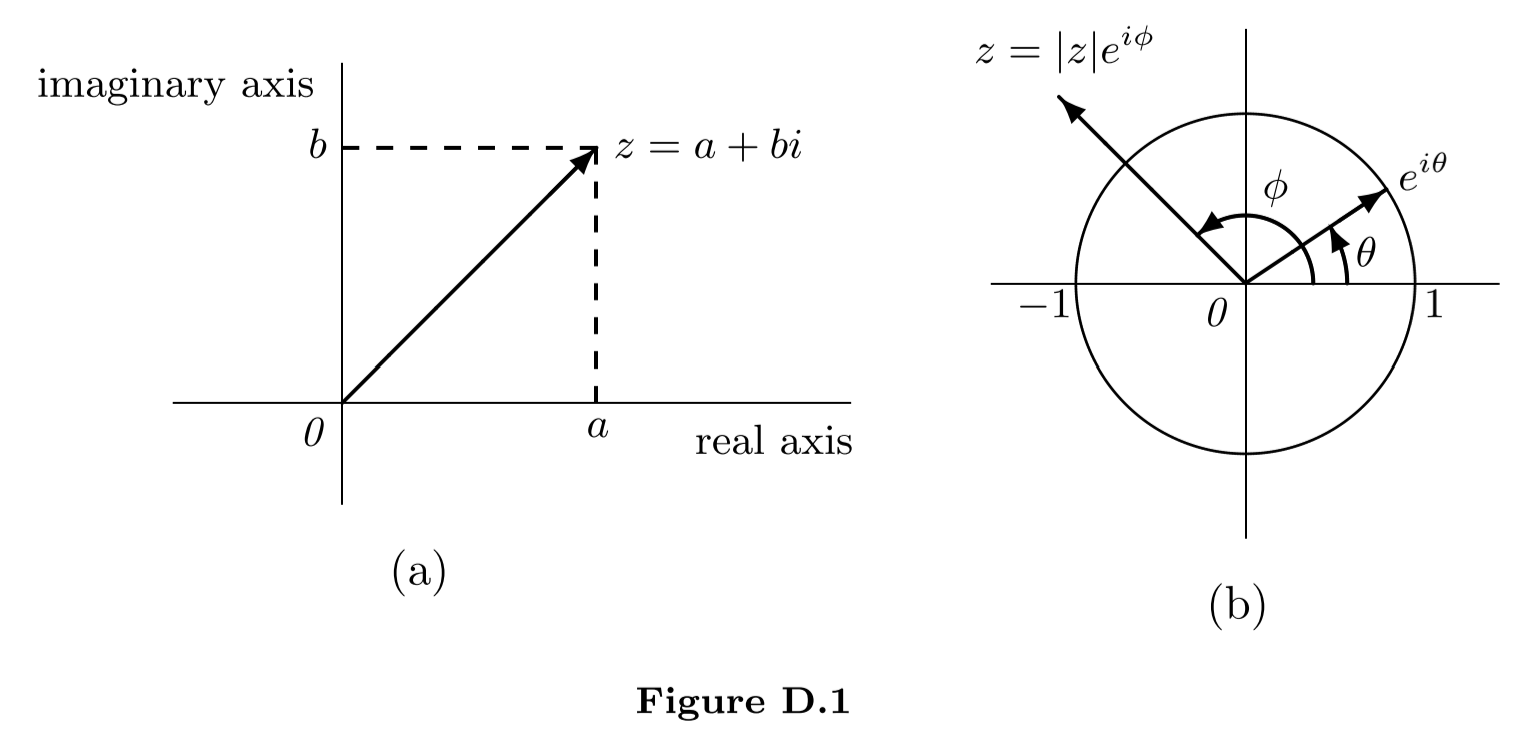
\includegraphics[width=14cm]{images/figure-d-1.png}

\begin{remark} \label{remark d.6}
It is interesting as well as \emph{useful} that complex numbers have both a \emph{geometric and an algebraic representation}.
Suppose that \(z = a + b\iu\), where \(a\) and \(b\) are real numbers.
We may \emph{represent} \(z\) as a vector in the \emph{complex plane} (see Figure D.1(a)).
Notice that, as in \(\SET{R}^2\), there are \emph{two axes}, the \textbf{real axis} and the \textbf{imaginary axis}.
The real and imaginary parts of \(z\) are the first and second coordinates, and the absolute value of \(z\) gives the \emph{length} of the vector \(z\).
It is clear that addition of complex numbers may be represented as in \(\SET{R}^2\) using the parallelogram law.
\end{remark}

\begin{remark} \label{remark d.7}
In \SEC{2.7}, we introduce \href{https://www.wikiwand.com/en/Euler\%27s_formula}{Euler's formula}.
The special case \(e^{\iu \theta} = \cos \theta + \iu \sin \theta\) is of particular interest.
Because of the geometry we have introduced, we may represent the vector \(e^{\iu \theta}\) as in Figure D.l(b);
that is, \(e^{\iu \theta}\) is the \emph{unit vector} that \emph{makes an angle \(\theta\) with the positive real axis}.

From this figure, we see that any \emph{nonzero} complex number \(z\) may be depicted as a multiple of a unit vector, namely, \(z = \abs{z}e^{\iu \phi}\), where \(\phi\) is the angle that the vector \(z\) makes with the positive real axis.
\textbf{Thus multiplication, as well as addition, has a simple geometric interpretation}:
If \(z = \abs{z} e^{\iu \theta}\) and \(w = \abs{w} e^{\iu \omega}\) are two nonzero complex numbers, then from the properties established in
\SEC{2.7} and \THM{d.3}, we have
\begin{align*}
    zw & = \abs{z} e^{\iu \theta} \cdot \abs{w} e^{\iu \omega} & \text{by supposition} \\
       & = \abs{z}\abs{w} e^{\iu \theta} e^{\iu \omega} & \text{of course} \\
       & = \abs{zw} e^{\iu \theta} e^{\iu \omega} & \text{by \THM{d.3}(a)} \\
       & = \abs{zw} e^{\iu (\theta + \omega)} & \text{just exponential algebra for complex numbers, see definition in page 133}
\end{align*}
So \(zw\) is the vector whose length is the product of the lengths of \(zw\), and makes the angle \(\theta + \omega\) with the positive real axis.
\end{remark}

Our \textbf{motivation} for enlarging the set of real numbers to the set of complex numbers is to obtain a field such that
\emph{every polynomial with nonzero degree having coefficients in that field has a zero}.
Our next result guarantees that the field of complex numbers has this property.

\begin{appendix theorem} [The Fundamental Theorem of Algebra] \label{thm d.4}
Suppose that \(p(z) = a_n z^n + a_{n-1} z^{n-1} + ... + a_1 z + a_0\) is a polynomial in \(\mathcal{P}(\SET{C})\) of
degree \(n \ge 1\).
Then \(p(z)\) has a zero.
\end{appendix theorem}

\begin{proof}
Please refer to some analysis course.
\end{proof}

The following important corollary is a consequence of \THM{d.4} and the \emph{division algorithm} for polynomials (\THM{e.1}).

\begin{appendix corollary} \label{corollary d.4.1}
If \(p(z) = a_n z^n + a_{n-1}z^{n - 1} + ... + a_1 z + a_0\) is a polynomial of degree \(n \ge 1\) with \emph{complex} coefficients, then there exist complex numbers \(c_1, c_2, ..., c_n\) (\emph{not} necessarily distinct) such that
\[
    p(z) = a_n(z - c_1)(z - c_2) ... (z - c_n).
\]
\end{appendix corollary}

\begin{proof}
If \(p(z)\) has degree \(1\), then \(p(z) = a_1 z + a_0 = a_1(z + \cfrac{a_0}{a_1})\), which has the desired form.

So assume \(p(z)\) has degree \(n > 1\).
WLOG, we can write \(p(z)\) as
\begin{align*}
    p(z) & = a_n z^n + a_{n-1}Z^{n - 1} + ... + a_1 z + a_0 \\
         & = a_n \left( z^n + \frac{a_{n-1}}{a_n} z^{n - 1} + ... + \frac{a_1}{a_n} z + \frac{a_0}{a_n} \right)
\end{align*}
Now by \THM{d.4}, \(z^n + \cfrac{a_{n-1}}{a_n} z^{n - 1} + ... + \cfrac{a_1}{a_n} z + \cfrac{a_0}{a_n}\) has a zero \(c_1\), so
\[
    z^n + \frac{a_{n-1}}{a_n} z^{n - 1} + ... + \frac{a_1}{a_n} z + \frac{a_0}{a_n} = (z - c_1)q_1(z)
\]
for some \(q_1(z)\) having degree \(n - 1\).
So we have
\[
    p(z) = a_n (z - c_1) q_1(z).
\]
Continue this process \emph{inductively} on \(q_1(z)\), we will get \(p(z) = a_n(z - c_1)(z - c_2) ... (z - c_n)\), as desired.
\end{proof}

\begin{remark} \label{remark d.8}
A field is called \textbf{algebraically closed} if it has the property that every polynomial of positive degree with coefficients from that field factors as a product of polynomials of degree \(1\).
Thus the preceding corollary asserts that the field of complex numbers is algebraically closed.
\end{remark}

\section{Polynomials} \label{sec 8.e}

In this appendix, we discuss some useful properties of the polynomials \emph{with coefficients from a field}.
For the definition of a polynomial, refer to \SEC{1.2}.
(See \ADEF{1.4}.)
Throughout this appendix, we assume that all polynomials have coefficients from a fixed field \(F\).

\begin{appendix definition} \label{def e.1}
A polynomial \(f(x)\) \textbf{divides} a polynomial \(g(x)\) if there exists a polynomial \(q(x)\) such that \(g(x) = f(x)q(x)\).
\end{appendix definition}

Our first result shows that the familiar long division process for polynomials \emph{with real} coefficients \textbf{is valid for} polynomials with coefficients from an \textbf{arbitrary field}.

\begin{appendix theorem} [The Division Algorithm for Polynomials] \label{thm e.1}
Let \(f(x)\) be a polynomial of degree \(n\), and let \(g(x)\) be a polynomial of degree \(m \ge 0\).
Then there \textbf{exist unique} polynomials \(q(x)\) and \(r(x)\) such that
\[
    f(x) = q(x)g(x) + r(x), \quad \quad \quad \MAROON{(1)}
\]
where the degree of \(r(x)\) is \emph{less than} \(m\).
\end{appendix theorem}

\begin{proof}
We begin by establishing the \emph{existence} of \(q(x)\) and \(r(x)\) that satisfy \MAROON{(1)}.
There are two cases:
\begin{enumerate}
\item[\BLUE{Case I}] If \(n < m\), take \(q(x) = 0\), having degree \(-1 < m\) by definition, and \(r(x) = f(x)\), then \MAROON{(1)} is satisfied.
\item[Case II] Otherwise, if \(0 \le m \le n\), we apply mathematical induction on \(n\).
\end{enumerate}

First, for the base case, suppose that \(n = 0\).
Then (since \(0 \le m \le n = 0\),) \(m = 0\), and it follows that \(f(x)\) and \(g(x)\) are \emph{nonzero} constants.
Hence we may take \(q(x) = f(x)/g(x)\) and \(r(x) = 0\) to satisfy \MAROON{(1)}.
(Note that \(q(x)\) is also a nonzero constant, and \(r(x)\) has degree \(-1 < 0 = m\).)

Now suppose that the result is valid for all polynomials with degree \emph{less than or equal to} \(n - 1\) for some fixed \(n > 0\).
And suppose \(f(x)\) is an arbitrary polynomial with degree \(n\), and let \(g(x)\) be a given arbitrary polynomial with degree \(0 \le m \le n\).
Suppose that \(f(x), g(x)\) has the form
\[
    f(x) = a_n x^n + a_{n - 1} x^{n - 1} + ... + a_1 x + a_0
\]
and
\[
    g(x) = b_m x^m + b_{m - 1} x^{m - 1} + ... + b_1 x + b_0.
\]
Then we have
\begin{align*}
    & a_n b_m^{-1} x^{n - m} g(x) \\
    & = (a_n b_m^{-1}) x^{n - m} (b_m x^m + b_{m - 1} x^{m - 1} + ... + b_1 x + b_0) \\
    & = \RED{a_n} x^n + a_n b_m^{-1} b_{m - 1} x^{n - 1} + ... + a_n b_m^{-1} b_1 x^{n - m + 1} + a_n b_m^{-1} b_0 x^{n - m}.
\end{align*}
So let \(h(x)\) be the polynomial defined by
\[
    h(x) = f(x) - a_n b_m^{-1} x^{n - m} g(x). \quad \quad \quad \MAROON{(2)}
\]
Then from the nasty equation above, \(h(x)\) is a polynomial of degree \(k < n\), since the coefficient of \(x^n\) is cancelled.
Now, if \(k\) is in fact also less than \(m\), then the relation between \(h(x)\) and \(g(x)\) again satisfies the \BLUE{Case I} in the beginning, so we can just take \(q_1(x) = 0\) and \(r(x) = h(x)\) such that \(h(x) = q_1(x)g(x) + r(x)\).
Otherwise, since \(k < n\), we still can apply the induction hypothesis to obtain polynomials \(q_1(x)\) and \(r(x)\) such that \(r(x)\) has degree less than \(m\), and
\[
    h(x) = q_1(x)g(x) + r(x). \quad \quad \quad \MAROON{(3)}
\]
Combining \MAROON{(2)} and \MAROON{(3)} and solving for \(f(x)\) gives us
\begin{align*}
    f(x) & = h(x) + a_n b_m^{-1} x^{n - m} g(x) & \text{by \MAROON{(2)}} \\
         & = q_1(x)g(x) + r(x) + a_n b_m^{-1} x^{n - m} g(x) & \text{by \MAROON{(3)}} \\
         & = \left[ q_1(x) + a_n b_m^{-1} x^{n - m} \right] \cdot g(x) + r(x) & \text{of course} \\
         & = q(x) \cdot g(x) + r(x),
\end{align*}
where \(q(x) = q_1(x) + a_n b_m^{-1} x^{n - m}\), and \(r(x)\) has degree less than \(m\), hence the existence of \(q(x)\) and \(r(x)\) by mathematical induction.

We now show the \textbf{uniqueness} of \(q(x)\) and \(r(x)\).
Suppose that \(q_1(x), q_2(x), r_1(x)\), and \(r_2(x)\) exist such that \(r_1(x)\) and \(r_2(x)\) each has degree less than \(m\) and
\[
    f(x) = q_1(x)g(x) + r_1(x) = q_2(x)g(x) + r_2(x).
\]
Then
\[
    [q_1(x)- q_2(x)]g(x) = r_2(x) - r_1(x). \quad \quad \quad \MAROON{(4)}
\]
Since both \(r_1(x)\) and \(r_2(x)\) have degree less than \(n\), \(r_2(x) - r_1(x)\) must have degree less than \(n\).
But since \(g(x)\) has degree \(m\), it must follow that \(q_1(x) - q_2(x)\) is the zero polynomial.
(Otherwise the product of \([q_1(x)- q_2(x)]g(x)\) has degree \(\ge m\) and is equal to \(r_2(x) - r_1(x)\) having degree less than \(m\), which is impossible.)
Hence \(q_1(x) = q_2(x)\), and the LHS of \MAROON{(4)} is zero polynomial, hence the RHS of \MAROON{(4)} is also the zero polynomial, and thus \(r_1(x) = r_2(x)\).
\end{proof}

\begin{remark} \label{remark e.1}
In the context of \THM{e.1}, we call \(q(x)\) and \(r(x)\) the \textbf{quotient} and \textbf{remainder}, respectively, for the division of \(f(x)\) by \(g(x)\).
For example, suppose that \(F\) is the field of complex numbers.
Then the quotient and remainder for the division of
\[
    f(x) = (3 + \iu)x^5 - (1 - \iu)x^4 + 6x^3 + (-6 + 2\iu)x^2 + (2 + \iu)x + 1
\]
by
\[
    g(x) = (3 + \iu)x^2 - 2\iu x + 4
\]
are, respectively,
\[
    q(x) = x^3 + \iu x^2 - 2 \quad \text{ and } \quad r(x) = (2 - 3\iu)x + 9.
\]
\end{remark}

\begin{appendix corollary} \label{corollary e.1.1}
Let \(f(x)\) be a polynomial of positive degree, and let \(a \in F\).
Then \(f(a) = 0\) if and only if \(x - a\) divides \(f(x)\).
\end{appendix corollary}

\begin{proof}
Suppose that \(x - a\) divides \(f(x)\).
Then there exists a polynomial \(q(x)\) such that \(f(x) = (x - a)q(x)\).
Thus \(f(a) = (a - a)q(a) = 0 \cdot q(a) = 0\).

Conversely, suppose that \(f(a) = 0\).
Then let \(g(x) = (x - a)\), having degree \RED{\(1\)}.
By the division algorithm, \THM{e.1}, there exist polynomials \(q(x)\) and \(r(x)\) such that \(r(x)\) has degree less than \RED{\(1\)} and
\[
    f(x) = q(x)g(x) + r(x) = q(x)(x - a) + r(x).
\]
Substituting \(a\) for \(x\) in the equation above, we obtain
\[
    0 = f(a) = q(a)(a - a) + r(a) = q(a) \cdot 0 + r(a) = r(a).
\]
So \(r(a) = 0\).
Since \(r(x)\) has degree less than \(1\), it must be the \emph{constant polynomial} \(r(x) = 0\).
Thus \(f(x) = q(x)(x - a)\).
\end{proof}

\begin{remark} \label{remark e.2}
For any polynomial \(f(x)\) with coefficients from a field \(F\), an element \(a \in F\) is called a \textbf{zero} of \(f(x)\) if \(f(a) = 0\).
With this terminology, \CORO{e.1.1} states that \(a\) is a zero of \(f(x)\) if and only if \(x - a\) divides \(f(x)\).
\end{remark}

\begin{appendix corollary} \label{corollary e.1.2}
Any polynomial of degree \(n \ge 1\) has at most \(n\) distinct zeros.
\end{appendix corollary}

\begin{proof}
The proof is by mathematical induction on \(n\).
The result is obvious if \(n = 1\).
Now suppose that the result is true for some positive integer \(n\), and let \(f(x)\) be a polynomial of degree \(n + 1\).
If \(f(x)\) \emph{has no} zeros, then there is nothing to prove.
Otherwise, if \(a\) is a zero of \(f(x)\), then by \CORO{e.1.1} we may write \(f(x) = (x - a)q(x)\) for some polynomial \(q(x)\).
Note that \(q(x)\) must be of degree \(n\);
therefore, by the induction hypothesis, \(q(x)\) can have at most \(n\) distinct zeros.
Since any zero of \(f(x)\) distinct from \(a\) is also a zero of \(q(x)\), it follows that \(f(x)\) can have at most \(n + 1\) distinct zeros.
\end{proof}

\begin{remark} \label{remark e.3}
Polynomials \emph{having no common divisors} arise naturally in the study of \emph{canonical forms}.
(See \CH{7}.)
\end{remark}

\begin{appendix definition} \label{def e.2}
Polynomials \(f_1(x), f_2(x), ..., f_n(x)\) are called \textbf{relatively prime} if no polynomial of \textbf{positive} degree divides \textbf{all of} them.
\end{appendix definition}

\begin{remark} \label{remark e.4}
Note that if \(f_1(x), f_2(x), ..., f_n(x)\) are relatively prime, it \textbf{does not} imply that any \(n - 1\) polynomials of them are relatively prime.
Some trivial example: \(f_1(x) = x + 1, f_2(x) = (x + 1)(x + 3), f_3(x) = x + 2\), then all of them are relatively prime, but \(f_1(x)\) and \(f_2(x)\) are not.
\end{remark}

For example, the polynomials with \emph{real} coefficients \(f(x) = x^2(x - 1)\) and \(h(x) = (x - 1)(x - 2)\) are not relatively prime because \(x - 1\) divides each of them.
On the other hand, consider \(f(x)\) and \(g(x) = (x - 2)(x - 3)\), which do not appear to have common factors.
Could other factorizations of \(f(x)\) and \(g(x)\) reveal a hidden common factor?
We will soon see (\THM{e.9}) that the preceding factors are \emph{the only ones}.
Thus \(f(x)\) and \(g(x)\) are relatively prime because they have no common factors of positive degree.

\begin{lemma} \label{lem e.1}
If \(f_1(x)\) and \(f_2(x)\) are relatively prime polynomials, there exist polynomials \(q_1(x)\) and \(q_2(x)\) such that
\[
    q_1(x) f_1(x) + q_2(x) f_2(x) = 1,
\]
where \(1\) denotes the constant polynomial with value \(1\).
\end{lemma}

\begin{note}
這個\ Lemma 有一個數論版本的。若\ \(a, b\) 互質,則存在整數\ \(x, y\) 使得\ \(ax + by = 1\)。
See \href{https://www.wikiwand.com/en/Extended_Euclidean_algorithm}{Extended Euclidean algorithm}。
\end{note}

\begin{proof}
Without loss of generality, assume that the degree of \(f_1(x)\) is greater than or equal to the degree of \(f_2(x)\).
The proof is by mathematical induction on the \emph{degree of \(f_2(x)\)}.
If \(f_2(x)\) has degree \(0\), then \(f_2(x)\) is a nonzero constant \(c\).
In this case, we can take \(q_1(x) = 0\) and \(q_2(x) = 1/c\), then
\[
    f_1(x) q_1(x) + f_2(x) q_2(x) = f_1(x) \cdot 0 + c \cdot \frac{1}{c} = 1.
\]

Now suppose that the theorem holds whenever the polynomial of lesser degree has degree \emph{less than} \(n\) for some positive integer \(n\).
We need to show the theorem holds for the case \(n\).

So again without loss of generality, assume that the degree of \(f_1(x)\) is greater than or equal to the degree of \(f_2(x)\),
and suppose that \(f_2(x)\) has degree \(n\).
By the division algorithm, \THM{e.1}, for \(f_1(x)\) and \(f_2(x)\), there exist polynomials \(q(x)\) and \(r(x)\) such that \(r(x)\) has degree less than \(n\) and
\[
    f_1(x) = q(x)f_2(x) + r(x) \quad \quad \quad \MAROON{(1)}
\]
Since \(f_1(x)\) and \(f_2(x)\) are relatively prime, \(r(x)\) is \emph{not} the zero polynomial.
We claim that \(f_2(x)\) and \(r(x)\) are relatively prime.
Suppose otherwise; then (by \DEF{e.2}) there exists a polynomial \(g(x)\) of \emph{positive} degree that divides both \(f_2(x)\) and \(r(x)\).
Hence, by \MAROON{(1)}, \(g(x)\) \emph{also divides} \(f_1(x)\), contradicting the fact that \(f_1(x)\) and \(f_2(x)\) are relatively prime.

Since \(r(x)\) has degree less than \(n\) and \(r(x)\) and \(f_2(x)\) are relatively prime,
we may apply the induction hypothesis to \(f_2(x)\) and \(r(x)\).
Thus there exist polynomials \(g_1(x)\) and \(g_2(x)\) such that
\[
    g_1(x) f_2(x) + g_2(x) r(x) = 1. \quad \quad \quad \MAROON{(2)}
\]
Combining \MAROON{(1)} and \MAROON{(2)}, we have
\begin{align*}
    1 & = g_1(x)f_2(x) + g_2(x)r(x) & \text{by \MAROON{(2)}} \\
      & = g_1(x)f_2(x) + g_2(x)[f_1(x) - q(x)f_2(x)] & \text{by \MAROON{(1)}} \\
      & = g_2(x) f_1(x) + [g_1(x) - g_2(x)q(x)]f_2(x) & \text{of course}
\end{align*}
Thus, setting \(q_1(x) = g_2(x)\) and \(q_2(x) = g_1(x) - g_2(x)q(x)\), we obtain the desired result.
\end{proof}

\begin{appendix theorem} \label{thm e.2}
If \(f_1(x), f_2(x), ..., f_n(x)\) are relatively prime polynomials, there exist polynomials \(q_1(x), q_2(x), ..., q_n(x)\) such that
\[
    q_1(x)f_1(x) + q_2(x)f_2(x) + ... + q_n(x)f_n(x) = 1,
\]
where \(1\) denotes the constant polynomial with value \(1\).
\end{appendix theorem}

\begin{proof}
The proof is by mathematical induction on \(n\), the number of polynomials.
And \LEM{e.1} establishes the case \(n = 2\).

Now assume the result is true for fewer than \(n\) polynomials, for some \(n \ge 3\).

So suppose we have \(n\) relatively prime polynomials \(f_1(x), f_2(x), ..., f_n(x)\).
We will first consider the trivial case where the first \(n - 1\) polynomials are \emph{also} relatively prime.
(Note that this may not necessarily true, see \RMK{e.4}.)
By the induction hypothesis, there exist polynomials \(q_1(x), q_2(x), ..., q_{n - 1}(x)\) such that
\[
    q_1(x)f_1(x) + q_2(x)f_2(x) + ... + q_{n-1}(x)f_{n-1}(x) = 1.
\]
Then just setting \(q_n(x) = 0\), the zero polynomial, we have
\[
    q_1(x)f_1(x) + q_2(x)f_n(x) + ... + q_{n-1}(x)f_{n-1}(x) + \RED{q_n(x)}f_n(x) = 1.
\]
which proves the result if the first \(n - 1\) polynomials are relatively prime.

Now suppose that the first \(n - 1\) polynomials are \textbf{not} relatively prime, and let \(g(x)\) be the \emph{monic polynomial}(see \DEF{e.4}) of maximum positive degree that \emph{divides} each of these polynomials \(f_1(x), ..., f_{n - 1}(x)\).
For \(k = 1, 2, ..., n - 1\), let \(h_k(x)\) be the polynomial defined, such that,
\[
    f_k(x) = g(x)h_k(x). \quad \quad \quad \MAROON{(1)}
\]
Then the polynomials \(h_1(x), h_2(x), ..., h_{n - 1}(x)\) are relatively prime.
(Otherwise \(g(x)\) does \emph{not} have the maximum positive degree, a contradiction!)
So by the induction hypothesis, there exist polynomials \(\phi_1(x), \phi_2(x), ..., \phi_{n-1}(x)\) such that
\[
    \phi_1(x)h_1(x) + \phi_2(x)h_2(x) + ... + \phi_{n-1}(x)h_{n - 1}(x) = 1.
\]
Multiplying both sides of this equation by \(g(x)\), we obtain
\begin{align*}
             & \phi_1(x)h_1(x)g(x) + \phi_2(x)h_2(x)g(x) + ... + \phi_{n-1}(x)h_{n - 1}(x)g(x) = g(x). \\
    \implies & \phi_1(x)f_1(x) + \phi_2(x)f_2(x) + ... + \phi_{n-1}(x)f_{n-1}(x) = g(x) \quad \quad \MAROON{(2)} & \text{by \MAROON{(1)}}
\end{align*}
Note that \(g(x)\) and \(f_n(x)\) are relatively prime.
(If \(g(x)\) and \(f_n(x)\) are \emph{not} relatively prime, then all \(f_1(x), ..., f_{n-1}(x), f_n(x)\) have the factor \(g(x)\), which implies \(f_1, ..., f_n\) are not relatively prime, again a contradiction.)
Hence (by \LEM{e.1}) there exist polynomials \(p(x)\) and \(q_n(x)\) such that
\[
    p(x)g(x) + q_n(x)f_n(x) = 1. \quad \quad \quad \MAROON{(3)}
\]

So finally, let \(q_i(x) = p(x)\phi_i(x)\) for \(i= 1, 2, ..., n \RED{- 1}\).
Then from \MAROON{(2)} and \MAROON{(3)} we have
\begin{align*}
    & q_1(x)f_1(x) + q_2(x)f_2(x) + ... + q_{n-1}(x)f_{n-1}(x) + q_n(x)f_n(x) \\
    & = p(x)\phi_1(x)f_1(x) + p(x)\phi_2(x)f_2(x) + ... + p(x)\phi_{n\RED{-1}}(x)f_{n\RED{-1}}(x) + q_n(x)f_n(x) \\
    & = p(x) [\phi_1(x)f_1(x) + \phi_2(x)f_2(x) + ... + \phi_{n-1}(x)f_{n-1}(x)] + q_n(x)f_n(x) & \text{of course} \\
    & = p(x) g(x) + q_n(x)f_n(x) & \text{by \MAROON{(2)}} \\
    & = p(x) g(x) + 1 - p(x)g(x) & \text{by \MAROON{(3)}} \\
    & = 1
\end{align*}
which completes the induction argument.
\end{proof}

\begin{example} \label{example e.1}
Let \(f_1(x) = x - 1\), \(f_2(x) = x^2 + x - 2\), \(f_3(x) = x^2 - x - 1\), and \(f_4(x) = x + 1\).
As polynomials \emph{with real} coefficients, \(f_1(x), f_2(x), f_3(x)\) and \(f_4(x)\) are relatively prime.
It is easily verified that the polynomials \(q_1(x) = -x^2, q_2(x) = x, q_3(x) = -3\), and \(q_4(x) = x - 2\) satisfy
\[
    q_1(x)f_1(x) + q_2(x)f_2(x) + q_3(x)f_3(x) + q_4(x)f_4(x) = 1,
\]
and hence these polynomials satisfy the conclusion of \THM{e.2}.
\end{example}

Throughout \CH{5}, \CH{6}, and \CH{7}, we consider linear operators that are \emph{polynomials in a particular operator \(\T\)} and matrices that are \emph{polynomials in a particular matrix \(A\)}.
For these operators and matrices, the following notation is convenient.

\begin{appendix definition} \label{def e.3}
Let
\[
    f(t) = a_0 + a_1 x + ... + a_n x^n
\]
be a polynomial with coefficients from a field \(F\).
If \(\T\) is a linear operator on a vector space \(\V\) \emph{over} \(F\), we define
\[
    f(\T) = a_0 \ITRAN{} + a_1 \T + ... + a_n \T^n.
\]
Similarly, if \(A\) is an \(n \X n\) matrix with entries from \(F\), we define
\[
    f(A) = a_0 I + a_1 A + ... + a_n A^n.
\]
\end{appendix definition}

\begin{example} \label{example e.2}
Let \(\T\) be the linear operator on \(\SET{R}^2\) defined by \(\T(a, b) = (2a + b, a - b)\), and let \(f(x) = x^2 + 2x - 3\).
It is easily checked that \(\T^2(a, b) = (5a + b, a + 2b)\); so
\begin{align*}
    f(\T)(a, b) & = (\T^2 + 2\T - 3\ITRAN{})(a, b) \\
        & = (5a + b, a + 2b) + (4a + 2b, 2a - 2b) - 3(a, b) = (6a + 3b, 3a - 3b).
\end{align*}
Similarly, if
\[
    A = \begin{pmatrix} 2 & 1 \\ 1 & -1 \end{pmatrix},
\]
then
\[
    f(A) = A^2 + 2A - 3I = \begin{pmatrix} 5 & 1 \\ 1 & 2 \end{pmatrix} + 2 \begin{pmatrix} 2 & 1 \\ 1 & -1 \end{pmatrix} - 3 \begin{pmatrix} 1 & 0 \\ 0 & 1 \end{pmatrix} = \begin{pmatrix} 6 & 3 \\ 3 & -3 \end{pmatrix}.
\]
\end{example}

The next three results use this notation.

\begin{appendix theorem} \label{thm e.3}
Let \(f(x)\) be a polynomial with coefficients from a field \(F\), and let \(\T\) be a linear operator on a vector space \(\V\) over \(F\).
Then the following statements are true.
\begin{enumerate}
\item \(f(\T)\) is a liner operator on \(\V\).
\item If \(\beta\) is a \emph{finite} ordered basis for \(\V\) and \(A = [\T]_{\beta}\), then \([f(\T)]_{\beta} = f(A)\).
\end{enumerate}
\end{appendix theorem}

\begin{proof}
Let
\[
    f(x) = a_0 + a_1 x + ... + a_n x^n.
\]
\begin{enumerate}
\item We have \(f(\T) = a_0 \ITRAN{} + a_1 \T + ... + a_n \T^n\) by \DEF{e.3}.
But since \(\T^i\) is linear for nonnegative integer \(i\), (using induction and the fact that the composition of linear operators is linear), \(f(\T)\) is in fact a linear combination of linear functions hence is also linear.

\item
First, by \THM{2.11} and induction we have
\[
     [\T^n]_{\beta} = ([\T]_{\beta})^n. \quad \quad \quad \MAROON{(1)}
\]
And
\begin{align*}
    [f(\T)]_{\beta} & = [a_0 \ITRAN{} + a_1 \T + ... + a_n \T^n]_{\beta} & \text{by \DEF{e.3}} \\
        & = a_0 [\ITRAN{}]_{\beta} + a_1 [\T]_{\beta} + ... + a_n [\T^n]_{\beta} & \text{by \THM{2.8}(a)(b)} \\
        & = a_0 I + a_1 A + ... + a_n A^n & \text{by \MAROON{(1)}} \\
        & = f(A) & \text{by \DEF{e.3}}
\end{align*}
\end{enumerate}
\end{proof}

\begin{appendix theorem} \label{thm e.4}
Let \(\T\) be a linear operator on a vector space \(\V\) over a field \(F\), and let \(A\) be a square matrix with entries from \(F\).
Then, for any polynomials \(f_1(x)\) and \(f_2(x)\) with coefficients from \(F\),
\begin{enumerate}
\item \(f_1(\T)f_2(\T) = f_2(\T)f_1(\T)\).
\item \(f_1(A)f_2(A) = f_2(A)f_1(A)\).
\end{enumerate}
\end{appendix theorem}

\begin{proof}
Since \(f_1(x)f_2(x) = f_2(x)f_1(x)\), it's intuitively true that \DEF{e.3} is also commutative.
Let
\[
    f_1(x) = \sum_{i = 0}^n a_i x^i \quad \text{ and } \quad f_2(x) = \sum_{j = 0}^m b_j x^j.
\]
Then since \(A^0 = I\) and \(\T^0 = \ITRAN{}\) by \ADEF{2.6} and \ADEF{2.7}, by \DEF{e.3} and these facts,
\[
    f_1(\T) = \sum_{i = 0}^n a_i \T^i \quad \text{ and } \quad f_2(\T) = \sum_{j = 0}^m b_j \T^j.
\]
and
\[
    f_1(A) = \sum_{i = 0}^n a_i A^i \quad \text{ and } \quad f_2(\T) = \sum_{j = 0}^m b_j A^j.
\]
Then
\begin{align*}
    f_1(\T) f_2(\T) & = \sum_{i = 0}^n a_i \T^i \sum_{j = 0}^m b_j \T^j \\
                    & = \sum_{i = 0}^n \sum_{j = 0}^m (a_i \T^i) (b_j \T^j) & \text{move ``constant'' into summation} \\
                    & = \sum_{j = 0}^m \sum_{i = 0}^n (a_i \T^i) (b_j \T^j) & \text{change order of finite summation} \\
                    & = \sum_{j = 0}^m \sum_{i = 0}^n (b_j \T^j) (a_i \T^i) & \text{of course by \CH{2}} \\
                    & = \sum_{j = 0}^m (b_j \T^j) \sum_{i = 0}^n (a_i \T^i) & \text{move ``constant'' out of summation} \\
                    & = f_2(\T) f_1(\T),
\end{align*}
and
\begin{align*}
    f_1(A) f_2(A) & = \sum_{i = 0}^n a_i A^i \sum_{j = 0}^m b_j A^j \\
                    & = \sum_{i = 0}^n \sum_{j = 0}^m (a_i A^i) (b_j A^j) & \text{move ``constant'' into summation} \\
                    & = \sum_{j = 0}^m \sum_{i = 0}^n (a_i A^i) (b_j A^j) & \text{change order of finite summation} \\
                    & = \sum_{j = 0}^m \sum_{i = 0}^n (b_j A^j) (a_i A^i) & \text{of course by \CH{2}} \\
                    & = \sum_{j = 0}^m (b_j A^j) \sum_{i = 0}^n (a_i A^i) & \text{move ``constant'' out of summation} \\
                    & = f_2(A) f_1(A),
\end{align*}
as desired.
\end{proof}

\begin{appendix theorem} \label{thm e.5}
Let \(\T\) be a linear operator on a vector space \(\V\) over a field \(F\), and let \(A\) be an \(n \X n\) matrix with entries from \(F\).
If \(f_1(x)\) and \(f_2(x)\) are \emph{relatively prime} polynomials with entries from \(F\), then there exist polynomials \(q_1(x)\) and \(q_2(x)\) with entries from \(F\) such that
\begin{enumerate}
\item \(q_1(\T)f_1(\T) + q_2(\T)f_2(\T) = \ITRAN{}\).
\item \(q_1(A)f_1(A) + q_2(A)f_2(A) = I\).
\end{enumerate}
\end{appendix theorem}

\begin{proof}
By \LEM{e.1}, there exists polynomials \(q_1(x), q_2(x)\) such that
\[
    q_1(x)f_1(x) + q_2(x)f_2(x) = 1.
\]
Then by applying \DEF{e.3}, we have
\[
    q_1(\T)f_1(\T) + q_2(\T)f_2(\T) = 1 \cdot \ITRAN{} = \ITRAN{}
\]
and
\[
    q_1(A)f_1(A) + q_2(A)f_2(A) = 1 \cdot I = I,
\]
as desired.
\end{proof}

\begin{remark} \label{remark e.5}
In \CH{5} and \CH{7}, we are concerned with determining when a linear operator \(\T\) on a finite-dimensional vector space can be \emph{diagonalized} and with finding a \emph{simple (canonical)} representation of \(\T\).
Both of these problems are \emph{affected by the factorization of a certain polynomial determined by \(\T\)}
(the \emph{\CPOLY{}} of \(\T\)).
In this setting, particular types of polynomials play an important role.
\end{remark}

\begin{appendix definition} \label{def e.4}
A polynomial \(f(x)\) With coefficients from a field \(F\) is called \textbf{monic} if its leading coefficient is \(1\).
If \(f(x)\) has positive degree and \emph{cannot be expressed as a product of polynomials} with coefficients from \(F\) such that each \emph{has positive degree}, then \(f(x)\) is called \textbf{irreducible}.
\end{appendix definition}

\begin{note}
這個定義就有點對應到質數在數論的定義。
\end{note}

\begin{remark} \label{remark e.6}
Observe that whether a polynomial is irreducible \textbf{depends on the field \(F\)} from which its coefficients come.
For example, \(f(x) = x^2 + 1\) is irreducible over the field of real numbers, but it is \emph{not} irreducible over the field of complex numbers since \(x^2 + 1 = (x + \iu)(x - \iu)\).
\textbf{Clearly any polynomial of degree \(1\) is irreducible.}
Moreover, for polynomials with coefficients from an \textbf{algebraically closed} field, the polynomials of degree \(1\) are \emph{the only} irreducible polynomials.
The following facts are easily established.
\end{remark}

\begin{appendix theorem} \label{thm e.6}
Let \(\phi(x)\) and \(f(x)\) be polynomials.
If \(\phi(x)\) is irreducible and \(\phi(x)\) does not divide \(f(x)\), then \(\phi(x)\) and \(f(x)\) are relatively prime.
\end{appendix theorem}

\begin{proof}
For the sake of contradiction, suppose \(\phi(x)\) is irreducible and \(\phi(x)\) does not divide \(f(x)\),
\textbf{but} \(\phi(x)\) and \(f(x)\) are \emph{not} relatively prime.
Then by \DEF{e.2} there exists \(g(x)\) with \emph{positive degree} s.t. \(g(x)\) divides both \(\phi(x)\) and \(f(x)\).
That is,
\[
    \phi(x) = g(x)h_1(x) \quad \MAROON{(1)} \text{ and } \quad f(x) = g(x)h_2(x) \quad \MAROON{(2)}
\]
for some polynomials \(h_1(x), h_2(x), g(x)\), where \(g(x)\) has positive degree.
Then we show a contradiction by splitting the cases of the degree of \(h_1(x)\).

If \(h_1(x)\) has positive degree, than by \MAROON{(1)}, \(\phi(x)\) is equal to the product of polynomials having positive degree, hence by \DEF{e.4} is \emph{not} irreducible, a contradiction;

If \(h_1(x)\) is the zero polynomial, then by \MAROON{(1)}, \(\phi(x)\) is also equal to zero polynomial, so by \DEF{e.4} again is \emph{not} irreducible, a contradiction;

Finally, suppose \(h_1(x)\) has degree \(0\) and \(h_1(x) = c\) for some nonzero constant \(c\).
Then from \MAROON{(1)}, we have \(\phi(x) = g(x) \cdot c\), hence \(g(x) = \phi(x) \cdot c^{-1}\) \quad \MAROON{(3)}.
And
\begin{align*}
    f(x) & = g(x)h_2(x) & \text{by \MAROON{(2)}} \\
         & = \phi(x) \cdot c^{-1} \cdot h_2(x), & \text{by \MAROON{(3)}}
\end{align*}
So \(\phi(x)\) \emph{divides} \(f(x)\), which again is a contradiction.

So in all cases, we have a contradiction.
So \(f(x)\) and \(\phi(x)\) must be relatively prime.
\end{proof}

\begin{appendix theorem} \label{thm e.7}
Given any two irreducible \textbf{monic} polynomials, if they are distinct, then they are relatively prime.
\end{appendix theorem}

\begin{note}
We need the polynomial to be monic, since if \(f(x)\) is irreducible, then \(2f(x)\) is also irreducible, and one of them cannot be monic;
\emph{but} \(2f(x) = 2 \cdot f(x)\), where \(2\) is a (degree \(0\)) constant polynomial, so by \DEF{e.1}, \(f(x)\) divides \(2f(x)\).

But this case is trivial and useless since \(f(x)\) and \(2f(x)\) still have the same degree, so we exclude it.
\end{note}

\begin{proof}
Let \(f_1(x)\) and \(f_2(x)\) be two distinct monic irreducible polynomials.
For the sake of contradiction, suppose they are \emph{not} relatively prime.
Then there exists \(g(x), h_1(x), h_2(x)\), where \(g(x)\) has positive degree, such that
\[
    f_1(x) = g(x) h_1(x) \quad \text{ and } \quad f_2(x) = g(x) h_2(x).
\]
Then we split by cases on the degree of \(h_1(x)\) and \(h_2(x)\).
If one of them has positive degree, then \(f_1(x)\) or \(f_2(x)\) is equal to the product of polynomials having positive degree, and is by definition not irreducible, a contradiction.

Else, if one of them is zero polynomial, then \(f_1(x)\) or \(f_2(x)\) is also equal to the zero polynomial and is by definition not irreducible, again a contradiction.

Finally, the remaining case is both \(h_1(x)\) and \(h_2(x)\) are degree-\(0\) polynomial and equal to constant \(c_1, c_2\) respectively, 
So we have
\[
    f_1(x) = c_1 g(x) \quad \text{ and } \quad f_2(x) = c_2 g(x), \quad \quad \MAROON{(1)}
\]
But since \(f_1(x)\) and \(f_2(x)\) are \textbf{monic}, it must be the case that \(c_1 = c_2\), for if \(c_1 \ne c_2\), then from \MAROON{(1)}, the leading coefficient of \(f_1(x)\) [\(f_2(x)\)] is the product of \(c_1\) [\(c_2\)] and the leading coefficient of \(g(x)\), and one of \(f_1(x)\) and \(f_2(x)\) cannot be monic.
But \MAROON{(1)} and \(c_1 = c_2\) imply \(f_1(x) = f_2(x)\), which contradicts that \(f_1(x)\) and \(f_2(x)\) are distinct.

So in all cases we get a contradiction.
Hence \(f_1(x)\) and \(f_2(x)\) must be relatively prime.
\end{proof}

\begin{appendix theorem} \label{thm e.8}
Let \(f(x), g(x)\), and \(\phi(x)\) be polynomials.
If \(\phi(x)\) is irreducible and divides the \emph{product} \(f(x)g(x)\) \BLUE{(1)}, \quad then \(\phi(x)\) divides \(f(x)\) or \(\phi(x)\) divides \(g(x)\).
\end{appendix theorem}

\begin{proof}
Suppose that \(\phi(x)\) does \emph{not} divide \(f(x)\). \BLUE{(2)} \quad
Then it suffices to show \(\phi(x)\) divides \(g(x)\).

First since \(\phi(x)\) is irreducible, with the supposition \BLUE{(2)}, by \THM{e.6}, \(\phi(x)\) and \(f(x)\) are relatively prime, and so by \THM{e.2}, there exist polynomials \(q_1(x)\) and \(q_2(x)\) such that
\[
    1 = q_1(x)\phi(x) + q_2(x)f(x).
\]
Multiplying both sides of this equation by \(g(x)\) yields
\[
    g(x) = q_1(x)\phi(x)g(x) + q_2(x) \RED{f(x)g(x)}. \quad \quad \quad \MAROON{(1)}
\]
Since by supposition \BLUE{(1)}, \(\phi(x)\) divides \(f(x)g(x)\), there is a polynomial \(h(x)\) such that \(f(x)g(x) = \phi(x)h(x)\). \MAROON{(2)} \quad
Thus
\begin{align*}
    g(x) & = q_1(x)\phi(x)g(x) + q_2(x) \RED{f(x)g(x)} & \text{by \MAROON{(1)}} \\
         & = q_1(x)\phi(x)g(x) + q_2(x) \RED{\phi(x)h(x)} & \text{by \MAROON{(2)}} \\
         & = \phi(x) [q_1(x)g(x) + q_2(x)h(x)] & \text{of course}
\end{align*}
So \(\phi(x)\) divides \(g(x)\).
\end{proof}

\begin{appendix corollary} \label{corollary e.8.1}
Let \(\phi(x), \phi_1(x), \phi_2(x), ..., \phi_n(x)\) be irreducible monic polynomials.
If \(\phi(x)\) divides the product \(\phi_1(x)\phi_2(x) ... \phi_n(x)\), then \(\phi(x) = \phi_i(x)\) for some \(i (i = 1, 2, ..., n)\).
\end{appendix corollary}

\begin{note}
In this case we have \(\phi(x) \RED{=} \phi_i(x)\), not just \(\phi(x)\) divides \(\phi_i(x)\), this is because that all \(\phi_i(x)\) are irreducible.
\end{note}

\begin{proof}
We prove the corollary by mathematical induction on \(n\).
For \(n = 1\), we have two irreducible monic polynomials \(\phi(x)\) and \(\phi_1(x)\);
and since \(\phi(x)\) divides \(\phi_1(x)\), they are \emph{not} relatively prime, so by (the contrapositive of) \THM{e.7}, \(\phi(x) = \phi_1(x)\).

Suppose then that for some \(n > 1\), the corollary is true for any irreducible polynomial \(\phi(x)\) and any \(n - 1\) irreducible monic polynomials; now again let \(\phi(x)\) be arbitrary irreducible polynomial and \(\phi_1(x), \phi_2(x), ..., \phi_n(x)\) be any \(n\) irreducible polynomials.
If \(\phi(x)\) divides
\[
    \phi_1(x)\phi_2(x)...\phi_n(x) = [\phi_1(x)\phi_2(x)...\phi_{n-1}(x)]\phi_n(x),
\]
then by \THM{e.8}, \(\phi(x)\) divides the product \(\phi_1(x)\phi_2(x) ... \phi_{n - 1}(x)\) or \(\phi(x)\) divides \(\phi_n(x)\).
In the first case, \(\phi = \phi_i(x)\) for some \(i (i = 1, 2, ..., n - 1)\) by the induction hypothesis;
in the second case, \(\phi(x) = \phi_n(x)\) again by (the contrapositive of) \THM{e.7}.
So the induction is true for \(n\).
\end{proof}

We are now able to establish \emph{the unique factorization theorem}, which is used throughout \CH{5} and \CH{7}.
This result states that every polynomial of positive degree is \emph{uniquely expressible} as a constant times a product of irreducible monic polynomials.

\begin{note}
就對應到數論的質因數分解。
\end{note}

\begin{appendix theorem} [Unique Factorization Theorem for Polynomials] \label{thm e.9}
For any polynomial \(f(x)\) of positive degree, there exist a unique constant \(c\), unique distinct irreducible monic polynomials \(\phi_1(x), \phi_2(x), ..., \phi_l(x)\), and unique positive integers \(n_1, n_2, ..., n_k\) such that
\[
    f(x) = c[\phi_1(x)]^{n_1}[\phi_2(x)]^{n_2}...[\phi_k(x)]^{n_k}.
\]
\end{appendix theorem}

\begin{proof}
We begin by showing the \textbf{existence} of such a factorization using mathematical induction on the degree of \(f(x)\).
If \(f(x)\) is of degree \(1\), then \(f(x) = ax + b\) for some constants \(a\) and \(b\) with \(a \ne 0\).
Setting \(\phi(x) = x + b/a\), we have \(f(x) = a\phi(x)\).
Since \(\phi(x)\) is an irreducible monic polynomial, the result is proved in this case.

Now suppose that the conclusion is true for any polynomial with positive degree less than some integer \(n > 1\), and let \(f(x)\) be a polynomial of degree \(n\).
Then
\[
    f(x) = a_n x^n + ... + a_1 x + a_0
\]
for some constants \(a_i\) with \(a_n \ne 0\).
If \(f(x)\) is irreducible, then
\[
    f(x) = a_n \left( x^n + \frac{a_{n-1}}{a_n} x^{n - 1} + ... + \frac{a_1}{a_n} x +  \frac{a_0}{a_n} \right)
\]
is a representation of \(f(x)\) as a product of \(a_{n}\) and an irreducible \emph{monic} polynomial.
If \(f(x)\) is not irreducible, then \(f(x) = g(x)h(x)\) for some polynomials \(g(x)\) and \(h(x)\), each of \emph{positive} degree \emph{less than} \(n\).
The induction hypothesis guarantees that both \(g(x)\) and \(h(x)\) factor as products of a constant and powers of distinct irreducible monic polynomials.
Consequently \(f(x) = g(x)h(x)\) also factors in this way.
Thus, in either case, \(f(x)\) can be factored as a product of a constant and powers of distinct irreducible monic polynomials.

It remains to establish the \textbf{uniqueness} of such a factorization.
Suppose that
\begin{align*}
    f(x) & = c[\phi_1(x)]^{n_1}[\phi_2(x)]^{n_2}...[\phi_k(x)]^{n_k} \\
         & = d[\psi_1(x)]^{m_1}[\psi_2(x)]^{m_2}...[\psi_r(x)]^{m_r}, \quad \quad \MAROON{(1)}
\end{align*}
where \(c\) and \(d\) are constants,
\(\phi_i(x)\) and \(\psi_j(x)\) are \RED{distinct} (this will be used later) irreducible monic polynomials, respectively,
and \(n_i\) and \(m_j\) are positive integers for \(i = 1, 2, ..., k\) and \(j = 1, 2, ..., r\).
Clearly both \(c\) and \(d\) must be the leading coefficient of \(f(x)\); hence \(c = d\).
Dividing by \(c\), we find that \MAROON{(1)} becomes
\[
    [\phi_1(x)]^{n_1}[\phi_2(x)]^{n_2}...[\phi_k(x)]^{n_k} = [\psi_1(x)]^{m_1}[\psi_2(x)]^{m_2}...[\psi_r(x)]^{m_r}. \quad \quad \MAROON{(2)}
\]
So \(\phi_i(x)\) divides the right side of \MAROON{(2)} for \(i = 1, 2, ..., k\).
Consequently, by \CORO{e.8.1}, each \(\phi_i(x)\) equals some \(\psi_j(x)\), and similarly,
each \(\psi_j(x)\) equals some \(\phi_j(x)\).
We conclude that \(r = k\) and that, by \emph{renumbering} if necessary,
\(\phi_i(x) = \psi_{\RED{i}}(x)\) for \(i = 1, 2, ..., k\). \MAROON{(3)}
So now it suffices to show \(n_i = m_i\) for all \(i = 1, 2, ..., k\).
For the sake of contradiction, suppose that \(n_i \ne m_i\) for some \(i\).
Without loss of generality, we may suppose that \(i = 1\) and \(n_1 > m_1\).
Then by \emph{canceling} \(\phi_1(x)^{m_1}\) from both sides of \MAROON{(2)}, and the fact \MAROON{(3)} that \(\phi_i(x) = \psi_(x)\), we obtain
\begin{align*}
    [\phi_1(x)]^{n_1 - m_1}[\phi_2(x)]^{n_2}...[\phi_k(x)]^{n_k} & = [\phi_1(x)]^{\RED{m_1 - m_1}}[\phi_2(x)]^{m_2}...[\phi_k(x)]^{m_k} \\
    & = [\phi_{\RED{2}}(x)]^{m_2}...[\phi_{\RED{k}}(x)]^{m_k} \quad \quad \MAROON{(4)}
\end{align*}
Since \(n_1 - m_1 > 0\), \(\phi_1(x)\) (of course) divides the left side of \MAROON{(4)} and hence divides the right side also.
So again by \CORO{e.8.1} \(\phi_1(x)\) is equal to one of the irreducible monic polynomial of the right side;
that is \(\phi_1(x) = \phi_i(x)\) for some \(i = \RED{2, ... , k}\).
But this contradicts that \(\phi_1(x), \phi_2(x), ..., \phi_k(x)\) are \RED{distinct}.
Hence the factorizations of \(f(x)\) in \MAROON{(1)} are the same.
\end{proof}

\begin{remark} \label{remark e.7}
It is often useful to regard a polynomial \(f(x) = a_n x^n + ... + a_1 x + a_0\) with coefficients from a field \(F\) \textbf{as a function} \(f: F \to F\).
In this case, the value of \(f\) at \(c \in F\) is \(f(c) = a_n c^n + ... + a_1 c + a_0\).
\emph{Unfortunately}, for \emph{arbitrary fields} there is not a one-to-one correspondence between polynomials and polynomial functions.
For example, if \(f(x) = x^2\) and \(g(x) = x\) are two polynomials \RED{over the field \(Z_2\)} (defined in \EXAMPLE{c.4}),
then \(f(x)\) and \(g(x)\) have different degrees and hence are \RED{not equal as polynomials}.
But (trivially) \(f(a) = g(a)\) for all \(a \in Z_2\), so that \(f\) and \(g\) are \RED{equal polynomial \emph{functions}}.
Our final result shows that \textbf{this anomaly cannot occur over an infinite field}.
\end{remark}

\begin{appendix theorem} \label{thm e.10}
Let \(f(x)\) and \(g(x)\) be polynomials with coefficients from an \emph{infinite} field \(F\).
If \(f(a) = g(a)\) for all \(a \in F\), then the polynomial \emph{functions} \(f(x)\) and \(g(x)\) are equal.
\end{appendix theorem}

\begin{proof}
Suppose that \(f(a) = g(a)\) for all \(a \in F\).
Define \(h(x) = f(x) - g(x)\), and suppose for the sake of contradiction that \(h(x)\) is of degree \(n \ge 1\).
Since \(f(x) - g(x)\) can only be a polynomial with degree at most \(n\), it follows from \CORO{e.1.2} that \(h(x)\) can have at most \(n\) zeroes. \MAROON{(1)}.
But
\[
    h(a) = f(a) - g(a) = 0
\]
for every \(a \in F\), hence \(h(x)\) has infinitely many zeroes, which contradicts \MAROON{(1)}.
Thus the degree of \(h(x)\) \(<= 0\), so \(h(x)\) must be a constant polynomial.
And since \(h(a) = 0\) for each \(a \in F\), it follows that \(h(x)\) is the zero polynomial.
Hence \(f(x) = g(x)\).
\end{proof}


\end{CJK*}
\end{document}
